\documentclass[twoside]{book}

% Packages required by doxygen
\usepackage{fixltx2e}
\usepackage{calc}
\usepackage{doxygen}
\usepackage{graphicx}
\usepackage[utf8]{inputenc}
\usepackage{makeidx}
\usepackage{multicol}
\usepackage{multirow}
\PassOptionsToPackage{warn}{textcomp}
\usepackage{textcomp}
\usepackage[nointegrals]{wasysym}
\usepackage[table]{xcolor}
\usepackage{ifpdf,ifxetex}

% Font selection
\usepackage[T1]{fontenc}
\usepackage[scaled=.90]{helvet}
\usepackage{courier}
\usepackage{amssymb}
\usepackage{sectsty}
\renewcommand{\familydefault}{\sfdefault}
\allsectionsfont{%
  \fontseries{bc}\selectfont%
  \color{darkgray}%
}
\renewcommand{\DoxyLabelFont}{%
  \fontseries{bc}\selectfont%
  \color{darkgray}%
}
\newcommand{\+}{\discretionary{\mbox{\scriptsize$\hookleftarrow$}}{}{}}

% Page & text layout
\usepackage{geometry}
\geometry{%
  a4paper,%
  top=2.5cm,%
  bottom=2.5cm,%
  left=2.5cm,%
  right=2.5cm%
}
\tolerance=750
\hfuzz=15pt
\hbadness=750
\setlength{\emergencystretch}{15pt}
\setlength{\parindent}{0cm}
\setlength{\parskip}{3ex plus 2ex minus 2ex}
\makeatletter
\renewcommand{\paragraph}{%
  \@startsection{paragraph}{4}{0ex}{-1.0ex}{1.0ex}{%
    \normalfont\normalsize\bfseries\SS@parafont%
  }%
}
\renewcommand{\subparagraph}{%
  \@startsection{subparagraph}{5}{0ex}{-1.0ex}{1.0ex}{%
    \normalfont\normalsize\bfseries\SS@subparafont%
  }%
}
\makeatother

% Headers & footers
\usepackage{fancyhdr}
\pagestyle{fancyplain}
\fancyhead[LE]{\fancyplain{}{\bfseries\thepage}}
\fancyhead[CE]{\fancyplain{}{}}
\fancyhead[RE]{\fancyplain{}{\bfseries\leftmark}}
\fancyhead[LO]{\fancyplain{}{\bfseries\rightmark}}
\fancyhead[CO]{\fancyplain{}{}}
\fancyhead[RO]{\fancyplain{}{\bfseries\thepage}}
\fancyfoot[LE]{\fancyplain{}{}}
\fancyfoot[CE]{\fancyplain{}{}}
\fancyfoot[RE]{\fancyplain{}{\bfseries\scriptsize Generated by Doxygen }}
\fancyfoot[LO]{\fancyplain{}{\bfseries\scriptsize Generated by Doxygen }}
\fancyfoot[CO]{\fancyplain{}{}}
\fancyfoot[RO]{\fancyplain{}{}}
\renewcommand{\footrulewidth}{0.4pt}
\renewcommand{\chaptermark}[1]{%
  \markboth{#1}{}%
}
\renewcommand{\sectionmark}[1]{%
  \markright{\thesection\ #1}%
}

% Indices & bibliography
\usepackage{natbib}
\usepackage[titles]{tocloft}
\setcounter{tocdepth}{3}
\setcounter{secnumdepth}{5}
\makeindex

% Hyperlinks (required, but should be loaded last)
\ifpdf
  \usepackage[pdftex,pagebackref=true]{hyperref}
\else
  \ifxetex
    \usepackage[pagebackref=true]{hyperref}
  \else
    \usepackage[ps2pdf,pagebackref=true]{hyperref}
  \fi
\fi
\ifpdf
  \DeclareUnicodeCharacter{207B}{${}^{-}$}% Superscript minus
  \DeclareUnicodeCharacter{C2B2}{${}^{2}$}% Superscript two
  \DeclareUnicodeCharacter{C2B3}{${}^{3}$}% Superscript three
\else
  \catcode`\⁻=13% Superscript minus
  \def⁻{${}^{-}$}
  \catcode`\²=13% Superscript two
  \def²{${}^{2}$}
  \catcode`\³=13% Superscript three
  \def³{${}^{3}$}
\fi

\hypersetup{%
  colorlinks=true,%
  linkcolor=blue,%
  citecolor=blue,%
  unicode%
}

% Custom commands
\newcommand{\clearemptydoublepage}{%
  \newpage{\pagestyle{empty}\cleardoublepage}%
}

\usepackage{caption}
\captionsetup{labelsep=space,justification=centering,font={bf},singlelinecheck=off,skip=4pt,position=top}

\renewcommand{\numberline}[1]{#1~}
%===== C O N T E N T S =====

\begin{document}

% Titlepage & ToC
\hypersetup{pageanchor=false,
             bookmarksnumbered=true,
             pdfencoding=unicode
            }
\pagenumbering{alph}
\begin{titlepage}
\vspace*{7cm}
\begin{center}%
{\Large “\+Colony\+Game\+Engine“ \\[1ex]\large 0.\+01 }\\
\vspace*{1cm}
{\large Generated by Doxygen 1.8.15}\\
\end{center}
\end{titlepage}
\clearemptydoublepage
\pagenumbering{roman}
\tableofcontents
\clearemptydoublepage
\pagenumbering{arabic}
\hypersetup{pageanchor=true}

%--- Begin generated contents ---
\chapter{Fast\+Noise}
\label{md___users__afromullet__documents__s_f_m_l__colony2__colony__fast_noise__r_e_a_d_m_e}
\Hypertarget{md___users__afromullet__documents__s_f_m_l__colony2__colony__fast_noise__r_e_a_d_m_e}
\mbox{\hyperlink{class_fast_noise}{Fast\+Noise}} is an open source noise generation library with a large collection of different noise algorithms. This library has been designed for realtime usage from the ground up, so has been optimised for speed without sacrificing noise quality.

This project started when my search to find a good noise library for procedural terrain generation concluded without an obvious choice. I enjoyed the options and customisation of Accidental Noise Library and the speed of Lib\+Noise, so many of the techniques from these libraries and the knowledge I gained from reading through their source has gone into creating \mbox{\hyperlink{class_fast_noise}{Fast\+Noise}}.

I have now also created \href{https://github.com/Auburns/FastNoiseSIMD}{\tt Fast\+Noise S\+I\+MD}, which utilises S\+I\+MD C\+PU instructions to gain huge performance boosts. It is slightly less flexible and cannot be converted to other languages, but if you can I would highly suggest using this for heavy noise generation loads.

\subsubsection*{Features}


\begin{DoxyItemize}
\item Value Noise 2D, 3D
\item Perlin Noise 2D, 3D
\item Simplex Noise 2D, 3D, 4D
\item Cubic Noise 2D, 3D
\item Gradient Perturb 2D, 3D
\item Multiple fractal options for all of the above
\item Cellular (Voronoi) Noise 2D, 3D
\item White Noise 2D, 3D, 4D
\item Supports floats or doubles
\end{DoxyItemize}

\subsubsection*{Wiki}

Usage and documentation available in wiki

\href{https://github.com/Auburns/FastNoise/wiki}{\tt Wiki Link}

\subsubsection*{Related repositories}


\begin{DoxyItemize}
\item \href{https://github.com/Auburns/FastNoise_CSharp}{\tt Fast\+Noise C\#}
\item \href{https://github.com/Auburns/FastNoise_Java}{\tt Fast\+Noise Java}
\item \href{https://github.com/Auburns/FastNoiseSIMD}{\tt Fast\+Noise S\+I\+MD}
\item \href{https://www.assetstore.unity3d.com/en/#!/content/70706}{\tt Fast\+Noise Unity}
\item \href{https://github.com/midgen/UnrealFastNoise}{\tt Unreal Fast\+Noise}
\end{DoxyItemize}

Credit to \href{https://github.com/jobtalle/CubicNoise}{\tt Cubic\+Noise} for the cubic noise algorithm

\subsection*{\mbox{\hyperlink{class_fast_noise}{Fast\+Noise}} Preview}

I have written a compact testing application for all the features included in \mbox{\hyperlink{class_fast_noise}{Fast\+Noise}} with a visual representation. I use this for development purposes and testing noise settings used in terrain generation.

Download links can be found in the \href{https://github.com/Auburns/FastNoise/releases}{\tt Releases Section}.



\section*{Performance Comparisons}

Using default noise settings on \mbox{\hyperlink{class_fast_noise}{Fast\+Noise}} and matching those settings across the other libraries where possible.

Timings below are x1000 ns to generate 32x32x32 points of noise on a single thread.


\begin{DoxyItemize}
\item C\+PU\+: Intel Xeon Skylake @ 2.\+0\+Ghz
\item Compiler\+: Intel 17.\+0 x64
\end{DoxyItemize}

\tabulinesep=1mm
\begin{longtabu}spread 0pt [c]{*{5}{|X[-1]}|}
\hline
\PBS\centering \cellcolor{\tableheadbgcolor}\textbf{ Noise Type  }&\PBS\centering \cellcolor{\tableheadbgcolor}\textbf{ \mbox{\hyperlink{class_fast_noise}{Fast\+Noise}}  }&\PBS\centering \cellcolor{\tableheadbgcolor}\textbf{ Fast\+Noise\+S\+I\+MD A\+V\+X2  }&\PBS\centering \cellcolor{\tableheadbgcolor}\textbf{ Lib\+Noise  }&\PBS\centering \cellcolor{\tableheadbgcolor}\textbf{ \mbox{\hyperlink{class_fast_noise}{Fast\+Noise}} 2D   }\\\cline{1-5}
\endfirsthead
\hline
\endfoot
\hline
\PBS\centering \cellcolor{\tableheadbgcolor}\textbf{ Noise Type  }&\PBS\centering \cellcolor{\tableheadbgcolor}\textbf{ \mbox{\hyperlink{class_fast_noise}{Fast\+Noise}}  }&\PBS\centering \cellcolor{\tableheadbgcolor}\textbf{ Fast\+Noise\+S\+I\+MD A\+V\+X2  }&\PBS\centering \cellcolor{\tableheadbgcolor}\textbf{ Lib\+Noise  }&\PBS\centering \cellcolor{\tableheadbgcolor}\textbf{ \mbox{\hyperlink{class_fast_noise}{Fast\+Noise}} 2D   }\\\cline{1-5}
\endhead
White Noise  &141  &9  &&111   \\\cline{1-5}
Value  &642  &152  &&361   \\\cline{1-5}
Perlin  &1002  &324  &1368  &473   \\\cline{1-5}
Simplex  &1194  &294  &&883   \\\cline{1-5}
Cellular  &2979  &1283  &58125  &1074   \\\cline{1-5}
Cubic  &2979  &952  &&858   \\\cline{1-5}
\end{longtabu}


Comparision of fractal performance \href{https://github.com/Auburns/FastNoiseSIMD/wiki/In-depth-SIMD-level}{\tt here}.

\section*{Examples}

\subsection*{Cellular Noise}







\subsection*{Fractal Noise}



\subsection*{Value Noise}



\subsection*{White Noise}



\subsection*{Gradient Perturb}







\section*{Any suggestions or questions welcome}
\chapter{Hierarchical Index}
\section{Class Hierarchy}
This inheritance list is sorted roughly, but not completely, alphabetically\+:\begin{DoxyCompactList}
\item \contentsline{section}{\+\_\+\+C\+A\+Ruleset}{\pageref{struct___c_a_ruleset}}{}
\item \contentsline{section}{\+\_\+\+Graph\+Connection}{\pageref{struct___graph_connection}}{}
\item \contentsline{section}{\+\_\+\+Pos\+Pair}{\pageref{struct___pos_pair}}{}
\item \contentsline{section}{Applied\+Force\+Effect}{\pageref{struct_applied_force_effect}}{}
\item \contentsline{section}{A\+Star\+Node}{\pageref{struct_a_star_node}}{}
\item \contentsline{section}{Attack\+Stats}{\pageref{struct_attack_stats}}{}
\item \contentsline{section}{Base\+Creature}{\pageref{class_base_creature}}{}
\item \contentsline{section}{Biome}{\pageref{class_biome}}{}
\item \contentsline{section}{Body\+Part}{\pageref{class_body_part}}{}
\item \contentsline{section}{Creature\+Body}{\pageref{class_creature_body}}{}
\item default\+\_\+dfs\+\_\+visitor\begin{DoxyCompactList}
\item \contentsline{section}{Anatomy\+\_\+\+Basic\+\_\+\+D\+F\+S\+\_\+\+Visitor}{\pageref{class_anatomy___basic___d_f_s___visitor}}{}
\item \contentsline{section}{Anatomy\+\_\+\+D\+F\+S\+\_\+\+Section\+\_\+\+Visitor}{\pageref{class_anatomy___d_f_s___section___visitor}}{}
\end{DoxyCompactList}
\item \contentsline{section}{Defense\+Stats}{\pageref{struct_defense_stats}}{}
\item Drawable\begin{DoxyCompactList}
\item \contentsline{section}{Entity\+Tile}{\pageref{class_entity_tile}}{}
\item \contentsline{section}{Map}{\pageref{class_map}}{}
\begin{DoxyCompactList}
\item \contentsline{section}{C\+A\+\_\+\+Map}{\pageref{class_c_a___map}}{}
\item \contentsline{section}{Noise\+Map}{\pageref{class_noise_map}}{}
\end{DoxyCompactList}
\end{DoxyCompactList}
\item \contentsline{section}{Examine\+Window}{\pageref{class_examine_window}}{}
\item \contentsline{section}{Example\+App\+Console}{\pageref{struct_example_app_console}}{}
\item \contentsline{section}{Example\+App\+Log}{\pageref{struct_example_app_log}}{}
\item \contentsline{section}{Fast\+Noise}{\pageref{class_fast_noise}}{}
\item \contentsline{section}{File\+Logger}{\pageref{class_file_logger}}{}
\item \contentsline{section}{Grid\+Location}{\pageref{struct_grid_location}}{}
\item \contentsline{section}{Im\+Gui\+Data\+Type\+Info}{\pageref{struct_im_gui_data_type_info}}{}
\item \contentsline{section}{Im\+Gui\+Plot\+Array\+Getter\+Data}{\pageref{struct_im_gui_plot_array_getter_data}}{}
\item \contentsline{section}{Im\+Gui\+Resize\+Grip\+Def}{\pageref{struct_im_gui_resize_grip_def}}{}
\item \contentsline{section}{Im\+Gui\+Style\+Var\+Info}{\pageref{struct_im_gui_style_var_info}}{}
\item \contentsline{section}{Item}{\pageref{class_item}}{}
\begin{DoxyCompactList}
\item \contentsline{section}{Armor}{\pageref{class_armor}}{}
\item \contentsline{section}{Weapon}{\pageref{class_weapon}}{}
\end{DoxyCompactList}
\item \contentsline{section}{Item\+Manager}{\pageref{class_item_manager}}{}
\item \contentsline{section}{Map\+Data}{\pageref{class_map_data}}{}
\item \contentsline{section}{Map\+Effect}{\pageref{class_map_effect}}{}
\item \contentsline{section}{Map\+Tile\+Parameters}{\pageref{struct_map_tile_parameters}}{}
\item \contentsline{section}{Material}{\pageref{class_material}}{}
\item \contentsline{section}{Player\+G\+UI}{\pageref{class_player_g_u_i}}{}
\item \contentsline{section}{Resource}{\pageref{class_resource}}{}
\begin{DoxyCompactList}
\item \contentsline{section}{Ore}{\pageref{class_ore}}{}
\item \contentsline{section}{Plant}{\pageref{class_plant}}{}
\begin{DoxyCompactList}
\item \contentsline{section}{Tree}{\pageref{class_tree}}{}
\end{DoxyCompactList}
\end{DoxyCompactList}
\item \contentsline{section}{Rewrite\+Rules}{\pageref{struct_rewrite_rules}}{}
\item \contentsline{section}{Selection\+Window}{\pageref{class_selection_window}}{}
\begin{DoxyCompactList}
\item \contentsline{section}{Equipment\+Window}{\pageref{class_equipment_window}}{}
\item \contentsline{section}{Inventory\+Window}{\pageref{class_inventory_window}}{}
\end{DoxyCompactList}
\item \contentsline{section}{Tile}{\pageref{class_tile}}{}
\item \contentsline{section}{Tile\+Identification\+Data}{\pageref{struct_tile_identification_data}}{}
\item \contentsline{section}{Tissue}{\pageref{class_tissue}}{}
\item Transformable\begin{DoxyCompactList}
\item \contentsline{section}{Entity\+Tile}{\pageref{class_entity_tile}}{}
\item \contentsline{section}{Map}{\pageref{class_map}}{}
\end{DoxyCompactList}
\item \contentsline{section}{Vision}{\pageref{class_vision}}{}
\item \contentsline{section}{Wound\+Calculations}{\pageref{class_wound_calculations}}{}
\item \contentsline{section}{Wound\+Rule}{\pageref{struct_wound_rule}}{}
\end{DoxyCompactList}

\chapter{Class Index}
\section{Class List}
Here are the classes, structs, unions and interfaces with brief descriptions\+:\begin{DoxyCompactList}
\item\contentsline{section}{\mbox{\hyperlink{struct___c_a_ruleset}{\+\_\+\+C\+A\+Ruleset}} }{\pageref{struct___c_a_ruleset}}{}
\item\contentsline{section}{\mbox{\hyperlink{struct___graph_connection}{\+\_\+\+Graph\+Connection}} }{\pageref{struct___graph_connection}}{}
\item\contentsline{section}{\mbox{\hyperlink{struct___pos_pair}{\+\_\+\+Pos\+Pair}} }{\pageref{struct___pos_pair}}{}
\item\contentsline{section}{\mbox{\hyperlink{class_anatomy___basic___d_f_s___visitor}{Anatomy\+\_\+\+Basic\+\_\+\+D\+F\+S\+\_\+\+Visitor}} }{\pageref{class_anatomy___basic___d_f_s___visitor}}{}
\item\contentsline{section}{\mbox{\hyperlink{class_anatomy___d_f_s___section___visitor}{Anatomy\+\_\+\+D\+F\+S\+\_\+\+Section\+\_\+\+Visitor}} }{\pageref{class_anatomy___d_f_s___section___visitor}}{}
\item\contentsline{section}{\mbox{\hyperlink{struct_applied_force_effect}{Applied\+Force\+Effect}} }{\pageref{struct_applied_force_effect}}{}
\item\contentsline{section}{\mbox{\hyperlink{class_armor}{Armor}} }{\pageref{class_armor}}{}
\item\contentsline{section}{\mbox{\hyperlink{struct_a_star_node}{A\+Star\+Node}} }{\pageref{struct_a_star_node}}{}
\item\contentsline{section}{\mbox{\hyperlink{struct_attack_stats}{Attack\+Stats}} }{\pageref{struct_attack_stats}}{}
\item\contentsline{section}{\mbox{\hyperlink{class_base_creature}{Base\+Creature}} }{\pageref{class_base_creature}}{}
\item\contentsline{section}{\mbox{\hyperlink{class_biome}{Biome}} }{\pageref{class_biome}}{}
\item\contentsline{section}{\mbox{\hyperlink{class_body_part}{Body\+Part}} }{\pageref{class_body_part}}{}
\item\contentsline{section}{\mbox{\hyperlink{class_c_a___map}{C\+A\+\_\+\+Map}} }{\pageref{class_c_a___map}}{}
\item\contentsline{section}{\mbox{\hyperlink{class_creature_body}{Creature\+Body}} }{\pageref{class_creature_body}}{}
\item\contentsline{section}{\mbox{\hyperlink{struct_defense_stats}{Defense\+Stats}} }{\pageref{struct_defense_stats}}{}
\item\contentsline{section}{\mbox{\hyperlink{class_entity_tile}{Entity\+Tile}} }{\pageref{class_entity_tile}}{}
\item\contentsline{section}{\mbox{\hyperlink{class_equipment_window}{Equipment\+Window}} }{\pageref{class_equipment_window}}{}
\item\contentsline{section}{\mbox{\hyperlink{class_examine_window}{Examine\+Window}} }{\pageref{class_examine_window}}{}
\item\contentsline{section}{\mbox{\hyperlink{struct_example_app_console}{Example\+App\+Console}} }{\pageref{struct_example_app_console}}{}
\item\contentsline{section}{\mbox{\hyperlink{struct_example_app_log}{Example\+App\+Log}} }{\pageref{struct_example_app_log}}{}
\item\contentsline{section}{\mbox{\hyperlink{class_fast_noise}{Fast\+Noise}} }{\pageref{class_fast_noise}}{}
\item\contentsline{section}{\mbox{\hyperlink{class_file_logger}{File\+Logger}} }{\pageref{class_file_logger}}{}
\item\contentsline{section}{\mbox{\hyperlink{struct_grid_location}{Grid\+Location}} }{\pageref{struct_grid_location}}{}
\item\contentsline{section}{\mbox{\hyperlink{struct_im_gui_data_type_info}{Im\+Gui\+Data\+Type\+Info}} }{\pageref{struct_im_gui_data_type_info}}{}
\item\contentsline{section}{\mbox{\hyperlink{struct_im_gui_plot_array_getter_data}{Im\+Gui\+Plot\+Array\+Getter\+Data}} }{\pageref{struct_im_gui_plot_array_getter_data}}{}
\item\contentsline{section}{\mbox{\hyperlink{struct_im_gui_resize_grip_def}{Im\+Gui\+Resize\+Grip\+Def}} }{\pageref{struct_im_gui_resize_grip_def}}{}
\item\contentsline{section}{\mbox{\hyperlink{struct_im_gui_style_var_info}{Im\+Gui\+Style\+Var\+Info}} }{\pageref{struct_im_gui_style_var_info}}{}
\item\contentsline{section}{\mbox{\hyperlink{class_inventory_window}{Inventory\+Window}} \\*Not created a parent class at the moment. Never made a G\+UI like this, and can\textquotesingle{}t accurately predict what will be reused until I implement a prototype. Trying to keep the function methods consitent so that I can add a parent class when needed }{\pageref{class_inventory_window}}{}
\item\contentsline{section}{\mbox{\hyperlink{class_item}{Item}} }{\pageref{class_item}}{}
\item\contentsline{section}{\mbox{\hyperlink{class_item_manager}{Item\+Manager}} }{\pageref{class_item_manager}}{}
\item\contentsline{section}{\mbox{\hyperlink{class_map}{Map}} }{\pageref{class_map}}{}
\item\contentsline{section}{\mbox{\hyperlink{class_map_data}{Map\+Data}} }{\pageref{class_map_data}}{}
\item\contentsline{section}{\mbox{\hyperlink{class_map_effect}{Map\+Effect}} }{\pageref{class_map_effect}}{}
\item\contentsline{section}{\mbox{\hyperlink{struct_map_tile_parameters}{Map\+Tile\+Parameters}} }{\pageref{struct_map_tile_parameters}}{}
\item\contentsline{section}{\mbox{\hyperlink{class_material}{Material}} }{\pageref{class_material}}{}
\item\contentsline{section}{\mbox{\hyperlink{class_noise_map}{Noise\+Map}} }{\pageref{class_noise_map}}{}
\item\contentsline{section}{\mbox{\hyperlink{class_ore}{Ore}} }{\pageref{class_ore}}{}
\item\contentsline{section}{\mbox{\hyperlink{class_plant}{Plant}} }{\pageref{class_plant}}{}
\item\contentsline{section}{\mbox{\hyperlink{class_player_g_u_i}{Player\+G\+UI}} }{\pageref{class_player_g_u_i}}{}
\item\contentsline{section}{\mbox{\hyperlink{class_resource}{Resource}} }{\pageref{class_resource}}{}
\item\contentsline{section}{\mbox{\hyperlink{struct_rewrite_rules}{Rewrite\+Rules}} }{\pageref{struct_rewrite_rules}}{}
\item\contentsline{section}{\mbox{\hyperlink{class_selection_window}{Selection\+Window}} }{\pageref{class_selection_window}}{}
\item\contentsline{section}{\mbox{\hyperlink{class_tile}{Tile}} }{\pageref{class_tile}}{}
\item\contentsline{section}{\mbox{\hyperlink{struct_tile_identification_data}{Tile\+Identification\+Data}} }{\pageref{struct_tile_identification_data}}{}
\item\contentsline{section}{\mbox{\hyperlink{class_tissue}{Tissue}} }{\pageref{class_tissue}}{}
\item\contentsline{section}{\mbox{\hyperlink{class_tree}{Tree}} }{\pageref{class_tree}}{}
\item\contentsline{section}{\mbox{\hyperlink{class_vision}{Vision}} }{\pageref{class_vision}}{}
\item\contentsline{section}{\mbox{\hyperlink{class_weapon}{Weapon}} }{\pageref{class_weapon}}{}
\item\contentsline{section}{\mbox{\hyperlink{class_wound_calculations}{Wound\+Calculations}} }{\pageref{class_wound_calculations}}{}
\item\contentsline{section}{\mbox{\hyperlink{struct_wound_rule}{Wound\+Rule}} }{\pageref{struct_wound_rule}}{}
\end{DoxyCompactList}

\chapter{File Index}
\section{File List}
Here is a list of all files with brief descriptions\+:\begin{DoxyCompactList}
\item\contentsline{section}{/\+Users/\+Afromullet/\+Documents/\+S\+F\+M\+L/\+Colony2/\+Colony/\mbox{\hyperlink{_debug_header_8h}{Debug\+Header.\+h}} }{\pageref{_debug_header_8h}}{}
\item\contentsline{section}{/\+Users/\+Afromullet/\+Documents/\+S\+F\+M\+L/\+Colony2/\+Colony/\mbox{\hyperlink{_filelogger_8cpp}{Filelogger.\+cpp}} }{\pageref{_filelogger_8cpp}}{}
\item\contentsline{section}{/\+Users/\+Afromullet/\+Documents/\+S\+F\+M\+L/\+Colony2/\+Colony/\mbox{\hyperlink{_filelogger_8hpp}{Filelogger.\+hpp}} }{\pageref{_filelogger_8hpp}}{}
\item\contentsline{section}{/\+Users/\+Afromullet/\+Documents/\+S\+F\+M\+L/\+Colony2/\+Colony/\mbox{\hyperlink{imgui__demo_8cpp}{imgui\+\_\+demo.\+cpp}} }{\pageref{imgui__demo_8cpp}}{}
\item\contentsline{section}{/\+Users/\+Afromullet/\+Documents/\+S\+F\+M\+L/\+Colony2/\+Colony/\mbox{\hyperlink{main_8cpp}{main.\+cpp}} }{\pageref{main_8cpp}}{}
\item\contentsline{section}{/\+Users/\+Afromullet/\+Documents/\+S\+F\+M\+L/\+Colony2/\+Colony/\mbox{\hyperlink{_pathfinding_8cpp}{Pathfinding.\+cpp}} }{\pageref{_pathfinding_8cpp}}{}
\item\contentsline{section}{/\+Users/\+Afromullet/\+Documents/\+S\+F\+M\+L/\+Colony2/\+Colony/\mbox{\hyperlink{_pathfinding_8hpp}{Pathfinding.\+hpp}} }{\pageref{_pathfinding_8hpp}}{}
\item\contentsline{section}{/\+Users/\+Afromullet/\+Documents/\+S\+F\+M\+L/\+Colony2/\+Colony/\mbox{\hyperlink{_resource_path_8hpp}{Resource\+Path.\+hpp}} }{\pageref{_resource_path_8hpp}}{}
\item\contentsline{section}{/\+Users/\+Afromullet/\+Documents/\+S\+F\+M\+L/\+Colony2/\+Colony/\mbox{\hyperlink{_resource_path_8mm}{Resource\+Path.\+mm}} }{\pageref{_resource_path_8mm}}{}
\item\contentsline{section}{/\+Users/\+Afromullet/\+Documents/\+S\+F\+M\+L/\+Colony2/\+Colony/\+Combat\+Handlers/\mbox{\hyperlink{_attack_handler_8cpp}{Attack\+Handler.\+cpp}} }{\pageref{_attack_handler_8cpp}}{}
\item\contentsline{section}{/\+Users/\+Afromullet/\+Documents/\+S\+F\+M\+L/\+Colony2/\+Colony/\+Combat\+Handlers/\mbox{\hyperlink{_attack_handler_8hpp}{Attack\+Handler.\+hpp}} }{\pageref{_attack_handler_8hpp}}{}
\item\contentsline{section}{/\+Users/\+Afromullet/\+Documents/\+S\+F\+M\+L/\+Colony2/\+Colony/\+Command\+Handlers/\mbox{\hyperlink{_key_definitions_8cpp}{Key\+Definitions.\+cpp}} }{\pageref{_key_definitions_8cpp}}{}
\item\contentsline{section}{/\+Users/\+Afromullet/\+Documents/\+S\+F\+M\+L/\+Colony2/\+Colony/\+Command\+Handlers/\mbox{\hyperlink{_key_definitions_8hpp}{Key\+Definitions.\+hpp}} }{\pageref{_key_definitions_8hpp}}{}
\item\contentsline{section}{/\+Users/\+Afromullet/\+Documents/\+S\+F\+M\+L/\+Colony2/\+Colony/\+Creature/\mbox{\hyperlink{_base_creature_8cpp}{Base\+Creature.\+cpp}} }{\pageref{_base_creature_8cpp}}{}
\item\contentsline{section}{/\+Users/\+Afromullet/\+Documents/\+S\+F\+M\+L/\+Colony2/\+Colony/\+Creature/\mbox{\hyperlink{_base_creature_8hpp}{Base\+Creature.\+hpp}} }{\pageref{_base_creature_8hpp}}{}
\item\contentsline{section}{/\+Users/\+Afromullet/\+Documents/\+S\+F\+M\+L/\+Colony2/\+Colony/\+Creature/\+Body/\mbox{\hyperlink{_body_graph_8cpp}{Body\+Graph.\+cpp}} }{\pageref{_body_graph_8cpp}}{}
\item\contentsline{section}{/\+Users/\+Afromullet/\+Documents/\+S\+F\+M\+L/\+Colony2/\+Colony/\+Creature/\+Body/\mbox{\hyperlink{_body_graph_8hpp}{Body\+Graph.\+hpp}} }{\pageref{_body_graph_8hpp}}{}
\item\contentsline{section}{/\+Users/\+Afromullet/\+Documents/\+S\+F\+M\+L/\+Colony2/\+Colony/\+Creature/\+Body/\mbox{\hyperlink{_body_graph_getters_8cpp}{Body\+Graph\+Getters.\+cpp}} }{\pageref{_body_graph_getters_8cpp}}{}
\item\contentsline{section}{/\+Users/\+Afromullet/\+Documents/\+S\+F\+M\+L/\+Colony2/\+Colony/\+Creature/\+Body/\mbox{\hyperlink{_body_graph_getters_8hpp}{Body\+Graph\+Getters.\+hpp}} }{\pageref{_body_graph_getters_8hpp}}{}
\item\contentsline{section}{/\+Users/\+Afromullet/\+Documents/\+S\+F\+M\+L/\+Colony2/\+Colony/\+Creature/\+Body/\mbox{\hyperlink{_body_part_8cpp}{Body\+Part.\+cpp}} }{\pageref{_body_part_8cpp}}{}
\item\contentsline{section}{/\+Users/\+Afromullet/\+Documents/\+S\+F\+M\+L/\+Colony2/\+Colony/\+Creature/\+Body/\mbox{\hyperlink{_body_part_8hpp}{Body\+Part.\+hpp}} }{\pageref{_body_part_8hpp}}{}
\item\contentsline{section}{/\+Users/\+Afromullet/\+Documents/\+S\+F\+M\+L/\+Colony2/\+Colony/\+Creature/\+Body/\mbox{\hyperlink{_tissue_8cpp}{Tissue.\+cpp}} }{\pageref{_tissue_8cpp}}{}
\item\contentsline{section}{/\+Users/\+Afromullet/\+Documents/\+S\+F\+M\+L/\+Colony2/\+Colony/\+Creature/\+Body/\mbox{\hyperlink{_tissue_8hpp}{Tissue.\+hpp}} }{\pageref{_tissue_8hpp}}{}
\item\contentsline{section}{/\+Users/\+Afromullet/\+Documents/\+S\+F\+M\+L/\+Colony2/\+Colony/\+Creature/\+Body/\mbox{\hyperlink{_wound_8cpp}{Wound.\+cpp}} }{\pageref{_wound_8cpp}}{}
\item\contentsline{section}{/\+Users/\+Afromullet/\+Documents/\+S\+F\+M\+L/\+Colony2/\+Colony/\+Creature/\+Body/\mbox{\hyperlink{_wound_8hpp}{Wound.\+hpp}} }{\pageref{_wound_8hpp}}{}
\item\contentsline{section}{/\+Users/\+Afromullet/\+Documents/\+S\+F\+M\+L/\+Colony2/\+Colony/\+Creature/\+Perception/\mbox{\hyperlink{_vision_8cpp}{Vision.\+cpp}} }{\pageref{_vision_8cpp}}{}
\item\contentsline{section}{/\+Users/\+Afromullet/\+Documents/\+S\+F\+M\+L/\+Colony2/\+Colony/\+Creature/\+Perception/\mbox{\hyperlink{_vision_8hpp}{Vision.\+hpp}} }{\pageref{_vision_8hpp}}{}
\item\contentsline{section}{/\+Users/\+Afromullet/\+Documents/\+S\+F\+M\+L/\+Colony2/\+Colony/\+Data/\mbox{\hyperlink{_data_storage_8cpp}{Data\+Storage.\+cpp}} }{\pageref{_data_storage_8cpp}}{}
\item\contentsline{section}{/\+Users/\+Afromullet/\+Documents/\+S\+F\+M\+L/\+Colony2/\+Colony/\+Data/\mbox{\hyperlink{_data_storage_8hpp}{Data\+Storage.\+hpp}} }{\pageref{_data_storage_8hpp}}{}
\item\contentsline{section}{/\+Users/\+Afromullet/\+Documents/\+S\+F\+M\+L/\+Colony2/\+Colony/\+Data/\mbox{\hyperlink{_material_8cpp}{Material.\+cpp}} }{\pageref{_material_8cpp}}{}
\item\contentsline{section}{/\+Users/\+Afromullet/\+Documents/\+S\+F\+M\+L/\+Colony2/\+Colony/\+Data/\mbox{\hyperlink{_material_8hpp}{Material.\+hpp}} }{\pageref{_material_8hpp}}{}
\item\contentsline{section}{/\+Users/\+Afromullet/\+Documents/\+S\+F\+M\+L/\+Colony2/\+Colony/\+Data/\+Data\+Readers/\mbox{\hyperlink{_data_readers_8cpp}{Data\+Readers.\+cpp}} }{\pageref{_data_readers_8cpp}}{}
\item\contentsline{section}{/\+Users/\+Afromullet/\+Documents/\+S\+F\+M\+L/\+Colony2/\+Colony/\+Data/\+Data\+Readers/\mbox{\hyperlink{_data_readers_8hpp}{Data\+Readers.\+hpp}} }{\pageref{_data_readers_8hpp}}{}
\item\contentsline{section}{/\+Users/\+Afromullet/\+Documents/\+S\+F\+M\+L/\+Colony2/\+Colony/\+Data/\+Data\+Readers/\mbox{\hyperlink{_generic_readers_8cpp}{Generic\+Readers.\+cpp}} }{\pageref{_generic_readers_8cpp}}{}
\item\contentsline{section}{/\+Users/\+Afromullet/\+Documents/\+S\+F\+M\+L/\+Colony2/\+Colony/\+Data/\+Data\+Readers/\mbox{\hyperlink{_generic_readers_8hpp}{Generic\+Readers.\+hpp}} }{\pageref{_generic_readers_8hpp}}{}
\item\contentsline{section}{/\+Users/\+Afromullet/\+Documents/\+S\+F\+M\+L/\+Colony2/\+Colony/\+Data/\+Data\+Readers/\mbox{\hyperlink{_history_token_reader_8cpp}{History\+Token\+Reader.\+cpp}} }{\pageref{_history_token_reader_8cpp}}{}
\item\contentsline{section}{/\+Users/\+Afromullet/\+Documents/\+S\+F\+M\+L/\+Colony2/\+Colony/\+Data/\+Data\+Readers/\mbox{\hyperlink{_history_token_reader_8hpp}{History\+Token\+Reader.\+hpp}} }{\pageref{_history_token_reader_8hpp}}{}
\item\contentsline{section}{/\+Users/\+Afromullet/\+Documents/\+S\+F\+M\+L/\+Colony2/\+Colony/\+Defs/\mbox{\hyperlink{_constants_8cpp}{Constants.\+cpp}} }{\pageref{_constants_8cpp}}{}
\item\contentsline{section}{/\+Users/\+Afromullet/\+Documents/\+S\+F\+M\+L/\+Colony2/\+Colony/\+Defs/\mbox{\hyperlink{_constants_8hpp}{Constants.\+hpp}} }{\pageref{_constants_8hpp}}{}
\item\contentsline{section}{/\+Users/\+Afromullet/\+Documents/\+S\+F\+M\+L/\+Colony2/\+Colony/\+Defs/\mbox{\hyperlink{_enum_types_8hpp}{Enum\+Types.\+hpp}} }{\pageref{_enum_types_8hpp}}{}
\item\contentsline{section}{/\+Users/\+Afromullet/\+Documents/\+S\+F\+M\+L/\+Colony2/\+Colony/\+Defs/\mbox{\hyperlink{_error_constants_8hpp}{Error\+Constants.\+hpp}} }{\pageref{_error_constants_8hpp}}{}
\item\contentsline{section}{/\+Users/\+Afromullet/\+Documents/\+S\+F\+M\+L/\+Colony2/\+Colony/\+Defs/\mbox{\hyperlink{_error_values_8hpp}{Error\+Values.\+hpp}} }{\pageref{_error_values_8hpp}}{}
\item\contentsline{section}{/\+Users/\+Afromullet/\+Documents/\+S\+F\+M\+L/\+Colony2/\+Colony/\+Defs/\mbox{\hyperlink{_globals_8cpp}{Globals.\+cpp}} }{\pageref{_globals_8cpp}}{}
\item\contentsline{section}{/\+Users/\+Afromullet/\+Documents/\+S\+F\+M\+L/\+Colony2/\+Colony/\+Defs/\mbox{\hyperlink{_globals_8hpp}{Globals.\+hpp}} }{\pageref{_globals_8hpp}}{}
\item\contentsline{section}{/\+Users/\+Afromullet/\+Documents/\+S\+F\+M\+L/\+Colony2/\+Colony/\+Defs/\mbox{\hyperlink{_s_f_m_l_overloaded_operators_8cpp}{S\+F\+M\+L\+Overloaded\+Operators.\+cpp}} }{\pageref{_s_f_m_l_overloaded_operators_8cpp}}{}
\item\contentsline{section}{/\+Users/\+Afromullet/\+Documents/\+S\+F\+M\+L/\+Colony2/\+Colony/\+Defs/\mbox{\hyperlink{_s_f_m_l_overloaded_operators_8hpp}{S\+F\+M\+L\+Overloaded\+Operators.\+hpp}} }{\pageref{_s_f_m_l_overloaded_operators_8hpp}}{}
\item\contentsline{section}{/\+Users/\+Afromullet/\+Documents/\+S\+F\+M\+L/\+Colony2/\+Colony/\+Defs/\mbox{\hyperlink{_static_var_initializer_8cpp}{Static\+Var\+Initializer.\+cpp}} }{\pageref{_static_var_initializer_8cpp}}{}
\item\contentsline{section}{/\+Users/\+Afromullet/\+Documents/\+S\+F\+M\+L/\+Colony2/\+Colony/\+Defs/\mbox{\hyperlink{_static_var_initializer_8hpp}{Static\+Var\+Initializer.\+hpp}} }{\pageref{_static_var_initializer_8hpp}}{}
\item\contentsline{section}{/\+Users/\+Afromullet/\+Documents/\+S\+F\+M\+L/\+Colony2/\+Colony/\+Defs/\mbox{\hyperlink{_util_macros_8h}{Util\+Macros.\+h}} }{\pageref{_util_macros_8h}}{}
\item\contentsline{section}{/\+Users/\+Afromullet/\+Documents/\+S\+F\+M\+L/\+Colony2/\+Colony/\+Equipment/\mbox{\hyperlink{_armor_8cpp}{Armor.\+cpp}} }{\pageref{_armor_8cpp}}{}
\item\contentsline{section}{/\+Users/\+Afromullet/\+Documents/\+S\+F\+M\+L/\+Colony2/\+Colony/\+Equipment/\mbox{\hyperlink{_armor_8hpp}{Armor.\+hpp}} }{\pageref{_armor_8hpp}}{}
\item\contentsline{section}{/\+Users/\+Afromullet/\+Documents/\+S\+F\+M\+L/\+Colony2/\+Colony/\+Equipment/\mbox{\hyperlink{_equipment_8cpp}{Equipment.\+cpp}} }{\pageref{_equipment_8cpp}}{}
\item\contentsline{section}{/\+Users/\+Afromullet/\+Documents/\+S\+F\+M\+L/\+Colony2/\+Colony/\+Equipment/\mbox{\hyperlink{_equipment_8hpp}{Equipment.\+hpp}} }{\pageref{_equipment_8hpp}}{}
\item\contentsline{section}{/\+Users/\+Afromullet/\+Documents/\+S\+F\+M\+L/\+Colony2/\+Colony/\+Equipment/\mbox{\hyperlink{_weapon_8cpp}{Weapon.\+cpp}} }{\pageref{_weapon_8cpp}}{}
\item\contentsline{section}{/\+Users/\+Afromullet/\+Documents/\+S\+F\+M\+L/\+Colony2/\+Colony/\+Equipment/\mbox{\hyperlink{_weapon_8hpp}{Weapon.\+hpp}} }{\pageref{_weapon_8hpp}}{}
\item\contentsline{section}{/\+Users/\+Afromullet/\+Documents/\+S\+F\+M\+L/\+Colony2/\+Colony/\+Fast\+Noise/\mbox{\hyperlink{_fast_noise_8cpp}{Fast\+Noise.\+cpp}} }{\pageref{_fast_noise_8cpp}}{}
\item\contentsline{section}{/\+Users/\+Afromullet/\+Documents/\+S\+F\+M\+L/\+Colony2/\+Colony/\+Fast\+Noise/\mbox{\hyperlink{_fast_noise_8h}{Fast\+Noise.\+h}} }{\pageref{_fast_noise_8h}}{}
\item\contentsline{section}{/\+Users/\+Afromullet/\+Documents/\+S\+F\+M\+L/\+Colony2/\+Colony/\+G\+U\+I/\mbox{\hyperlink{_imgui_debug_8cpp}{Imgui\+Debug.\+cpp}} }{\pageref{_imgui_debug_8cpp}}{}
\item\contentsline{section}{/\+Users/\+Afromullet/\+Documents/\+S\+F\+M\+L/\+Colony2/\+Colony/\+G\+U\+I/\mbox{\hyperlink{_imgui_debug_8hpp}{Imgui\+Debug.\+hpp}} }{\pageref{_imgui_debug_8hpp}}{}
\item\contentsline{section}{/\+Users/\+Afromullet/\+Documents/\+S\+F\+M\+L/\+Colony2/\+Colony/\+G\+U\+I/\mbox{\hyperlink{_player_windows_8cpp}{Player\+Windows.\+cpp}} }{\pageref{_player_windows_8cpp}}{}
\item\contentsline{section}{/\+Users/\+Afromullet/\+Documents/\+S\+F\+M\+L/\+Colony2/\+Colony/\+G\+U\+I/\mbox{\hyperlink{_player_windows_8hpp}{Player\+Windows.\+hpp}} }{\pageref{_player_windows_8hpp}}{}
\item\contentsline{section}{/\+Users/\+Afromullet/\+Documents/\+S\+F\+M\+L/\+Colony2/\+Colony/\+Handlers/\mbox{\hyperlink{_material_handlers_8cpp}{Material\+Handlers.\+cpp}} }{\pageref{_material_handlers_8cpp}}{}
\item\contentsline{section}{/\+Users/\+Afromullet/\+Documents/\+S\+F\+M\+L/\+Colony2/\+Colony/\+Handlers/\mbox{\hyperlink{_material_handlers_8hpp}{Material\+Handlers.\+hpp}} }{\pageref{_material_handlers_8hpp}}{}
\item\contentsline{section}{/\+Users/\+Afromullet/\+Documents/\+S\+F\+M\+L/\+Colony2/\+Colony/\+Handlers/\mbox{\hyperlink{_movement_handler_8cpp}{Movement\+Handler.\+cpp}} }{\pageref{_movement_handler_8cpp}}{}
\item\contentsline{section}{/\+Users/\+Afromullet/\+Documents/\+S\+F\+M\+L/\+Colony2/\+Colony/\+Handlers/\mbox{\hyperlink{_movement_handler_8hpp}{Movement\+Handler.\+hpp}} }{\pageref{_movement_handler_8hpp}}{}
\item\contentsline{section}{/\+Users/\+Afromullet/\+Documents/\+S\+F\+M\+L/\+Colony2/\+Colony/\+History/\mbox{\hyperlink{_history_generator_8cpp}{History\+Generator.\+cpp}} }{\pageref{_history_generator_8cpp}}{}
\item\contentsline{section}{/\+Users/\+Afromullet/\+Documents/\+S\+F\+M\+L/\+Colony2/\+Colony/\+History/\mbox{\hyperlink{_history_generator_8hpp}{History\+Generator.\+hpp}} }{\pageref{_history_generator_8hpp}}{}
\item\contentsline{section}{/\+Users/\+Afromullet/\+Documents/\+S\+F\+M\+L/\+Colony2/\+Colony/imgui/\mbox{\hyperlink{imgui-_s_f_m_l_8cpp}{imgui-\/\+S\+F\+M\+L.\+cpp}} }{\pageref{imgui-_s_f_m_l_8cpp}}{}
\item\contentsline{section}{/\+Users/\+Afromullet/\+Documents/\+S\+F\+M\+L/\+Colony2/\+Colony/imgui/\mbox{\hyperlink{imgui_8cpp}{imgui.\+cpp}} }{\pageref{imgui_8cpp}}{}
\item\contentsline{section}{/\+Users/\+Afromullet/\+Documents/\+S\+F\+M\+L/\+Colony2/\+Colony/imgui/\mbox{\hyperlink{imgui__draw_8cpp}{imgui\+\_\+draw.\+cpp}} }{\pageref{imgui__draw_8cpp}}{}
\item\contentsline{section}{/\+Users/\+Afromullet/\+Documents/\+S\+F\+M\+L/\+Colony2/\+Colony/\+Includes/\mbox{\hyperlink{_equipment___includes_8h}{Equipment\+\_\+\+Includes.\+h}} }{\pageref{_equipment___includes_8h}}{}
\item\contentsline{section}{/\+Users/\+Afromullet/\+Documents/\+S\+F\+M\+L/\+Colony2/\+Colony/\+Includes/\mbox{\hyperlink{_universal___includes_8h}{Universal\+\_\+\+Includes.\+h}} }{\pageref{_universal___includes_8h}}{}
\item\contentsline{section}{/\+Users/\+Afromullet/\+Documents/\+S\+F\+M\+L/\+Colony2/\+Colony/\+Input/\mbox{\hyperlink{_player_controls_8cpp}{Player\+Controls.\+cpp}} }{\pageref{_player_controls_8cpp}}{}
\item\contentsline{section}{/\+Users/\+Afromullet/\+Documents/\+S\+F\+M\+L/\+Colony2/\+Colony/\+Input/\mbox{\hyperlink{_player_controls_8hpp}{Player\+Controls.\+hpp}} }{\pageref{_player_controls_8hpp}}{}
\item\contentsline{section}{/\+Users/\+Afromullet/\+Documents/\+S\+F\+M\+L/\+Colony2/\+Colony/\+Managers/\mbox{\hyperlink{_item_manager_8cpp}{Item\+Manager.\+cpp}} }{\pageref{_item_manager_8cpp}}{}
\item\contentsline{section}{/\+Users/\+Afromullet/\+Documents/\+S\+F\+M\+L/\+Colony2/\+Colony/\+Managers/\mbox{\hyperlink{_item_manager_8hpp}{Item\+Manager.\+hpp}} }{\pageref{_item_manager_8hpp}}{}
\item\contentsline{section}{/\+Users/\+Afromullet/\+Documents/\+S\+F\+M\+L/\+Colony2/\+Colony/\+Map\+Components/\mbox{\hyperlink{_entity_tile_8cpp}{Entity\+Tile.\+cpp}} }{\pageref{_entity_tile_8cpp}}{}
\item\contentsline{section}{/\+Users/\+Afromullet/\+Documents/\+S\+F\+M\+L/\+Colony2/\+Colony/\+Map\+Components/\mbox{\hyperlink{_entity_tile_8hpp}{Entity\+Tile.\+hpp}} }{\pageref{_entity_tile_8hpp}}{}
\item\contentsline{section}{/\+Users/\+Afromullet/\+Documents/\+S\+F\+M\+L/\+Colony2/\+Colony/\+Map\+Components/\mbox{\hyperlink{_map_8cpp}{Map.\+cpp}} }{\pageref{_map_8cpp}}{}
\item\contentsline{section}{/\+Users/\+Afromullet/\+Documents/\+S\+F\+M\+L/\+Colony2/\+Colony/\+Map\+Components/\mbox{\hyperlink{_map_8hpp}{Map.\+hpp}} }{\pageref{_map_8hpp}}{}
\item\contentsline{section}{/\+Users/\+Afromullet/\+Documents/\+S\+F\+M\+L/\+Colony2/\+Colony/\+Map\+Components/\mbox{\hyperlink{_map_data_8cpp}{Map\+Data.\+cpp}} }{\pageref{_map_data_8cpp}}{}
\item\contentsline{section}{/\+Users/\+Afromullet/\+Documents/\+S\+F\+M\+L/\+Colony2/\+Colony/\+Map\+Components/\mbox{\hyperlink{_map_data_8hpp}{Map\+Data.\+hpp}} }{\pageref{_map_data_8hpp}}{}
\item\contentsline{section}{/\+Users/\+Afromullet/\+Documents/\+S\+F\+M\+L/\+Colony2/\+Colony/\+Map\+Components/\mbox{\hyperlink{_map_effect_8cpp}{Map\+Effect.\+cpp}} }{\pageref{_map_effect_8cpp}}{}
\item\contentsline{section}{/\+Users/\+Afromullet/\+Documents/\+S\+F\+M\+L/\+Colony2/\+Colony/\+Map\+Components/\mbox{\hyperlink{_map_effect_8hpp}{Map\+Effect.\+hpp}} }{\pageref{_map_effect_8hpp}}{}
\item\contentsline{section}{/\+Users/\+Afromullet/\+Documents/\+S\+F\+M\+L/\+Colony2/\+Colony/\+Map\+Components/\mbox{\hyperlink{_map_util_8cpp}{Map\+Util.\+cpp}} }{\pageref{_map_util_8cpp}}{}
\item\contentsline{section}{/\+Users/\+Afromullet/\+Documents/\+S\+F\+M\+L/\+Colony2/\+Colony/\+Map\+Components/\mbox{\hyperlink{_map_util_8hpp}{Map\+Util.\+hpp}} }{\pageref{_map_util_8hpp}}{}
\item\contentsline{section}{/\+Users/\+Afromullet/\+Documents/\+S\+F\+M\+L/\+Colony2/\+Colony/\+Map\+Components/\mbox{\hyperlink{_tile_8cpp}{Tile.\+cpp}} }{\pageref{_tile_8cpp}}{}
\item\contentsline{section}{/\+Users/\+Afromullet/\+Documents/\+S\+F\+M\+L/\+Colony2/\+Colony/\+Map\+Components/\mbox{\hyperlink{_tile_8hpp}{Tile.\+hpp}} }{\pageref{_tile_8hpp}}{}
\item\contentsline{section}{/\+Users/\+Afromullet/\+Documents/\+S\+F\+M\+L/\+Colony2/\+Colony/\+Map\+Components/\+Biome/\mbox{\hyperlink{_biomes_8cpp}{Biomes.\+cpp}} }{\pageref{_biomes_8cpp}}{}
\item\contentsline{section}{/\+Users/\+Afromullet/\+Documents/\+S\+F\+M\+L/\+Colony2/\+Colony/\+Map\+Components/\+Biome/\mbox{\hyperlink{_biomes_8hpp}{Biomes.\+hpp}} }{\pageref{_biomes_8hpp}}{}
\item\contentsline{section}{/\+Users/\+Afromullet/\+Documents/\+S\+F\+M\+L/\+Colony2/\+Colony/\+Map\+Components/\+Map\+Variants/\mbox{\hyperlink{_c_a_map_8cpp}{C\+A\+Map.\+cpp}} }{\pageref{_c_a_map_8cpp}}{}
\item\contentsline{section}{/\+Users/\+Afromullet/\+Documents/\+S\+F\+M\+L/\+Colony2/\+Colony/\+Map\+Components/\+Map\+Variants/\mbox{\hyperlink{_c_a_map_8hpp}{C\+A\+Map.\+hpp}} }{\pageref{_c_a_map_8hpp}}{}
\item\contentsline{section}{/\+Users/\+Afromullet/\+Documents/\+S\+F\+M\+L/\+Colony2/\+Colony/\+Map\+Components/\+Map\+Variants/\mbox{\hyperlink{_noise_map_8cpp}{Noise\+Map.\+cpp}} }{\pageref{_noise_map_8cpp}}{}
\item\contentsline{section}{/\+Users/\+Afromullet/\+Documents/\+S\+F\+M\+L/\+Colony2/\+Colony/\+Map\+Components/\+Map\+Variants/\mbox{\hyperlink{_noise_map_8hpp}{Noise\+Map.\+hpp}} }{\pageref{_noise_map_8hpp}}{}
\item\contentsline{section}{/\+Users/\+Afromullet/\+Documents/\+S\+F\+M\+L/\+Colony2/\+Colony/\+Resources/\mbox{\hyperlink{_ore_8cpp}{Ore.\+cpp}} }{\pageref{_ore_8cpp}}{}
\item\contentsline{section}{/\+Users/\+Afromullet/\+Documents/\+S\+F\+M\+L/\+Colony2/\+Colony/\+Resources/\mbox{\hyperlink{_ore_8hpp}{Ore.\+hpp}} }{\pageref{_ore_8hpp}}{}
\item\contentsline{section}{/\+Users/\+Afromullet/\+Documents/\+S\+F\+M\+L/\+Colony2/\+Colony/\+Resources/\mbox{\hyperlink{_plant_8cpp}{Plant.\+cpp}} }{\pageref{_plant_8cpp}}{}
\item\contentsline{section}{/\+Users/\+Afromullet/\+Documents/\+S\+F\+M\+L/\+Colony2/\+Colony/\+Resources/\mbox{\hyperlink{_plant_8hpp}{Plant.\+hpp}} }{\pageref{_plant_8hpp}}{}
\item\contentsline{section}{/\+Users/\+Afromullet/\+Documents/\+S\+F\+M\+L/\+Colony2/\+Colony/\+Resources/\mbox{\hyperlink{_resource_8cpp}{Resource.\+cpp}} }{\pageref{_resource_8cpp}}{}
\item\contentsline{section}{/\+Users/\+Afromullet/\+Documents/\+S\+F\+M\+L/\+Colony2/\+Colony/\+Resources/\mbox{\hyperlink{_resource_8hpp}{Resource.\+hpp}} }{\pageref{_resource_8hpp}}{}
\item\contentsline{section}{/\+Users/\+Afromullet/\+Documents/\+S\+F\+M\+L/\+Colony2/\+Colony/\+Resources/\mbox{\hyperlink{_tree_8cpp}{Tree.\+cpp}} }{\pageref{_tree_8cpp}}{}
\item\contentsline{section}{/\+Users/\+Afromullet/\+Documents/\+S\+F\+M\+L/\+Colony2/\+Colony/\+Resources/\mbox{\hyperlink{_tree_8hpp}{Tree.\+hpp}} }{\pageref{_tree_8hpp}}{}
\item\contentsline{section}{/\+Users/\+Afromullet/\+Documents/\+S\+F\+M\+L/\+Colony2/\+Colony/\+Testing/\mbox{\hyperlink{_combat_testing_8cpp}{Combat\+Testing.\+cpp}} }{\pageref{_combat_testing_8cpp}}{}
\item\contentsline{section}{/\+Users/\+Afromullet/\+Documents/\+S\+F\+M\+L/\+Colony2/\+Colony/\+Testing/\mbox{\hyperlink{_combat_testing_8hpp}{Combat\+Testing.\+hpp}} }{\pageref{_combat_testing_8hpp}}{}
\item\contentsline{section}{/\+Users/\+Afromullet/\+Documents/\+S\+F\+M\+L/\+Colony2/\+Colony/\+Testing/\mbox{\hyperlink{_item_generator_8cpp}{Item\+Generator.\+cpp}} }{\pageref{_item_generator_8cpp}}{}
\item\contentsline{section}{/\+Users/\+Afromullet/\+Documents/\+S\+F\+M\+L/\+Colony2/\+Colony/\+Testing/\mbox{\hyperlink{_item_generator_8hpp}{Item\+Generator.\+hpp}} }{\pageref{_item_generator_8hpp}}{}
\item\contentsline{section}{/\+Users/\+Afromullet/\+Documents/\+S\+F\+M\+L/\+Colony2/\+Colony/\+Testing/\mbox{\hyperlink{_test_data_generator_8cpp}{Test\+Data\+Generator.\+cpp}} }{\pageref{_test_data_generator_8cpp}}{}
\item\contentsline{section}{/\+Users/\+Afromullet/\+Documents/\+S\+F\+M\+L/\+Colony2/\+Colony/\+Testing/\mbox{\hyperlink{_test_data_generator_8hpp}{Test\+Data\+Generator.\+hpp}} }{\pageref{_test_data_generator_8hpp}}{}
\item\contentsline{section}{/\+Users/\+Afromullet/\+Documents/\+S\+F\+M\+L/\+Colony2/\+Colony/\+Tile\+Data/\mbox{\hyperlink{_tile_reader_8cpp}{Tile\+Reader.\+cpp}} }{\pageref{_tile_reader_8cpp}}{}
\item\contentsline{section}{/\+Users/\+Afromullet/\+Documents/\+S\+F\+M\+L/\+Colony2/\+Colony/\+Tile\+Data/\mbox{\hyperlink{_tile_reader_8hpp}{Tile\+Reader.\+hpp}} }{\pageref{_tile_reader_8hpp}}{}
\end{DoxyCompactList}

\chapter{Class Documentation}
\hypertarget{struct___c_a_ruleset}{}\section{\+\_\+\+C\+A\+Ruleset Struct Reference}
\label{struct___c_a_ruleset}\index{\+\_\+\+C\+A\+Ruleset@{\+\_\+\+C\+A\+Ruleset}}


{\ttfamily \#include $<$C\+A\+Map.\+hpp$>$}



Collaboration diagram for \+\_\+\+C\+A\+Ruleset\+:
\nopagebreak
\begin{figure}[H]
\begin{center}
\leavevmode
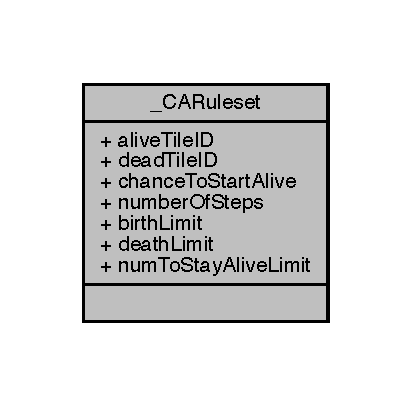
\includegraphics[width=197pt]{d2/d8a/struct___c_a_ruleset__coll__graph}
\end{center}
\end{figure}
\subsection*{Public Attributes}
\begin{DoxyCompactItemize}
\item 
int \mbox{\hyperlink{struct___c_a_ruleset_a337222bac7553157120b52380f58d570}{alive\+Tile\+ID}}
\item 
int \mbox{\hyperlink{struct___c_a_ruleset_a6d57373433d4eb5236bbeac8bb6f464f}{dead\+Tile\+ID}}
\item 
float \mbox{\hyperlink{struct___c_a_ruleset_afeb8028018113d49b14b5e19f7287d76}{chance\+To\+Start\+Alive}}
\item 
int \mbox{\hyperlink{struct___c_a_ruleset_ac2f4cb85d2b3e775e33eaed281a92b2d}{number\+Of\+Steps}}
\item 
int \mbox{\hyperlink{struct___c_a_ruleset_ab00fdee694e9ffe768885de7e5deb47e}{birth\+Limit}}
\item 
int \mbox{\hyperlink{struct___c_a_ruleset_a421ce30ec54473bec500e3374911637c}{death\+Limit}}
\item 
int \mbox{\hyperlink{struct___c_a_ruleset_a8af594e5e229ec31c0ef86b9bf214401}{num\+To\+Stay\+Alive\+Limit}}
\end{DoxyCompactItemize}


\subsection{Member Data Documentation}
\mbox{\Hypertarget{struct___c_a_ruleset_a337222bac7553157120b52380f58d570}\label{struct___c_a_ruleset_a337222bac7553157120b52380f58d570}} 
\index{\+\_\+\+C\+A\+Ruleset@{\+\_\+\+C\+A\+Ruleset}!alive\+Tile\+ID@{alive\+Tile\+ID}}
\index{alive\+Tile\+ID@{alive\+Tile\+ID}!\+\_\+\+C\+A\+Ruleset@{\+\_\+\+C\+A\+Ruleset}}
\subsubsection{\texorpdfstring{alive\+Tile\+ID}{aliveTileID}}
{\footnotesize\ttfamily int \+\_\+\+C\+A\+Ruleset\+::alive\+Tile\+ID}

\mbox{\Hypertarget{struct___c_a_ruleset_ab00fdee694e9ffe768885de7e5deb47e}\label{struct___c_a_ruleset_ab00fdee694e9ffe768885de7e5deb47e}} 
\index{\+\_\+\+C\+A\+Ruleset@{\+\_\+\+C\+A\+Ruleset}!birth\+Limit@{birth\+Limit}}
\index{birth\+Limit@{birth\+Limit}!\+\_\+\+C\+A\+Ruleset@{\+\_\+\+C\+A\+Ruleset}}
\subsubsection{\texorpdfstring{birth\+Limit}{birthLimit}}
{\footnotesize\ttfamily int \+\_\+\+C\+A\+Ruleset\+::birth\+Limit}

\mbox{\Hypertarget{struct___c_a_ruleset_afeb8028018113d49b14b5e19f7287d76}\label{struct___c_a_ruleset_afeb8028018113d49b14b5e19f7287d76}} 
\index{\+\_\+\+C\+A\+Ruleset@{\+\_\+\+C\+A\+Ruleset}!chance\+To\+Start\+Alive@{chance\+To\+Start\+Alive}}
\index{chance\+To\+Start\+Alive@{chance\+To\+Start\+Alive}!\+\_\+\+C\+A\+Ruleset@{\+\_\+\+C\+A\+Ruleset}}
\subsubsection{\texorpdfstring{chance\+To\+Start\+Alive}{chanceToStartAlive}}
{\footnotesize\ttfamily float \+\_\+\+C\+A\+Ruleset\+::chance\+To\+Start\+Alive}

\mbox{\Hypertarget{struct___c_a_ruleset_a6d57373433d4eb5236bbeac8bb6f464f}\label{struct___c_a_ruleset_a6d57373433d4eb5236bbeac8bb6f464f}} 
\index{\+\_\+\+C\+A\+Ruleset@{\+\_\+\+C\+A\+Ruleset}!dead\+Tile\+ID@{dead\+Tile\+ID}}
\index{dead\+Tile\+ID@{dead\+Tile\+ID}!\+\_\+\+C\+A\+Ruleset@{\+\_\+\+C\+A\+Ruleset}}
\subsubsection{\texorpdfstring{dead\+Tile\+ID}{deadTileID}}
{\footnotesize\ttfamily int \+\_\+\+C\+A\+Ruleset\+::dead\+Tile\+ID}

\mbox{\Hypertarget{struct___c_a_ruleset_a421ce30ec54473bec500e3374911637c}\label{struct___c_a_ruleset_a421ce30ec54473bec500e3374911637c}} 
\index{\+\_\+\+C\+A\+Ruleset@{\+\_\+\+C\+A\+Ruleset}!death\+Limit@{death\+Limit}}
\index{death\+Limit@{death\+Limit}!\+\_\+\+C\+A\+Ruleset@{\+\_\+\+C\+A\+Ruleset}}
\subsubsection{\texorpdfstring{death\+Limit}{deathLimit}}
{\footnotesize\ttfamily int \+\_\+\+C\+A\+Ruleset\+::death\+Limit}

\mbox{\Hypertarget{struct___c_a_ruleset_ac2f4cb85d2b3e775e33eaed281a92b2d}\label{struct___c_a_ruleset_ac2f4cb85d2b3e775e33eaed281a92b2d}} 
\index{\+\_\+\+C\+A\+Ruleset@{\+\_\+\+C\+A\+Ruleset}!number\+Of\+Steps@{number\+Of\+Steps}}
\index{number\+Of\+Steps@{number\+Of\+Steps}!\+\_\+\+C\+A\+Ruleset@{\+\_\+\+C\+A\+Ruleset}}
\subsubsection{\texorpdfstring{number\+Of\+Steps}{numberOfSteps}}
{\footnotesize\ttfamily int \+\_\+\+C\+A\+Ruleset\+::number\+Of\+Steps}

\mbox{\Hypertarget{struct___c_a_ruleset_a8af594e5e229ec31c0ef86b9bf214401}\label{struct___c_a_ruleset_a8af594e5e229ec31c0ef86b9bf214401}} 
\index{\+\_\+\+C\+A\+Ruleset@{\+\_\+\+C\+A\+Ruleset}!num\+To\+Stay\+Alive\+Limit@{num\+To\+Stay\+Alive\+Limit}}
\index{num\+To\+Stay\+Alive\+Limit@{num\+To\+Stay\+Alive\+Limit}!\+\_\+\+C\+A\+Ruleset@{\+\_\+\+C\+A\+Ruleset}}
\subsubsection{\texorpdfstring{num\+To\+Stay\+Alive\+Limit}{numToStayAliveLimit}}
{\footnotesize\ttfamily int \+\_\+\+C\+A\+Ruleset\+::num\+To\+Stay\+Alive\+Limit}



The documentation for this struct was generated from the following file\+:\begin{DoxyCompactItemize}
\item 
/\+Users/\+Afromullet/\+Documents/\+S\+F\+M\+L/\+Colony2/\+Colony/\+Map\+Components/\+Map\+Variants/\mbox{\hyperlink{_c_a_map_8hpp}{C\+A\+Map.\+hpp}}\end{DoxyCompactItemize}

\hypertarget{struct___graph_connection}{}\section{\+\_\+\+Graph\+Connection Struct Reference}
\label{struct___graph_connection}\index{\+\_\+\+Graph\+Connection@{\+\_\+\+Graph\+Connection}}


{\ttfamily \#include $<$Body\+Graph.\+hpp$>$}



Collaboration diagram for \+\_\+\+Graph\+Connection\+:\nopagebreak
\begin{figure}[H]
\begin{center}
\leavevmode
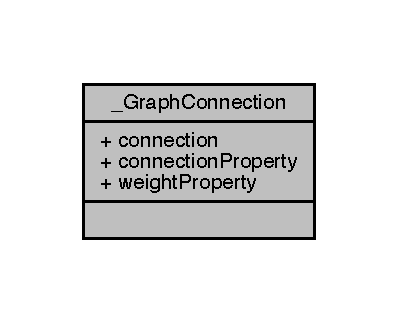
\includegraphics[width=191pt]{d6/d38/struct___graph_connection__coll__graph}
\end{center}
\end{figure}
\subsection*{Public Attributes}
\begin{DoxyCompactItemize}
\item 
\mbox{\hyperlink{_body_graph_8hpp_a1a9cb52373e2881d50e8971ff4a37803}{En\+Connection\+Type}} \mbox{\hyperlink{struct___graph_connection_a3111812a1c3863ecfb33757dce869efe}{connection}}
\item 
\mbox{\hyperlink{_body_graph_8hpp_aaf075ead75a7b8171312447a8e13aab8}{En\+Connection\+Property}} \mbox{\hyperlink{struct___graph_connection_ab4f55b760335b06eb893f9abded06939}{connection\+Property}}
\item 
\mbox{\hyperlink{_body_graph_8hpp_aca4f327513ae6b3eeddfb5d9ccff4eb7}{Edge\+Weight\+Prop}} \mbox{\hyperlink{struct___graph_connection_a243a1a161c39bafe16a580f2fca162d1}{weight\+Property}}
\end{DoxyCompactItemize}


\subsection{Member Data Documentation}
\mbox{\Hypertarget{struct___graph_connection_a3111812a1c3863ecfb33757dce869efe}\label{struct___graph_connection_a3111812a1c3863ecfb33757dce869efe}} 
\index{\+\_\+\+Graph\+Connection@{\+\_\+\+Graph\+Connection}!connection@{connection}}
\index{connection@{connection}!\+\_\+\+Graph\+Connection@{\+\_\+\+Graph\+Connection}}
\subsubsection{\texorpdfstring{connection}{connection}}
{\footnotesize\ttfamily \mbox{\hyperlink{_body_graph_8hpp_a1a9cb52373e2881d50e8971ff4a37803}{En\+Connection\+Type}} \+\_\+\+Graph\+Connection\+::connection}

\mbox{\Hypertarget{struct___graph_connection_ab4f55b760335b06eb893f9abded06939}\label{struct___graph_connection_ab4f55b760335b06eb893f9abded06939}} 
\index{\+\_\+\+Graph\+Connection@{\+\_\+\+Graph\+Connection}!connection\+Property@{connection\+Property}}
\index{connection\+Property@{connection\+Property}!\+\_\+\+Graph\+Connection@{\+\_\+\+Graph\+Connection}}
\subsubsection{\texorpdfstring{connection\+Property}{connectionProperty}}
{\footnotesize\ttfamily \mbox{\hyperlink{_body_graph_8hpp_aaf075ead75a7b8171312447a8e13aab8}{En\+Connection\+Property}} \+\_\+\+Graph\+Connection\+::connection\+Property}

\mbox{\Hypertarget{struct___graph_connection_a243a1a161c39bafe16a580f2fca162d1}\label{struct___graph_connection_a243a1a161c39bafe16a580f2fca162d1}} 
\index{\+\_\+\+Graph\+Connection@{\+\_\+\+Graph\+Connection}!weight\+Property@{weight\+Property}}
\index{weight\+Property@{weight\+Property}!\+\_\+\+Graph\+Connection@{\+\_\+\+Graph\+Connection}}
\subsubsection{\texorpdfstring{weight\+Property}{weightProperty}}
{\footnotesize\ttfamily \mbox{\hyperlink{_body_graph_8hpp_aca4f327513ae6b3eeddfb5d9ccff4eb7}{Edge\+Weight\+Prop}} \+\_\+\+Graph\+Connection\+::weight\+Property}



The documentation for this struct was generated from the following file\+:\begin{DoxyCompactItemize}
\item 
/\+Users/\+Afromullet/\+Documents/\+S\+F\+M\+L/\+Colony2/\+Colony/\+Creature/\+Body/\mbox{\hyperlink{_body_graph_8hpp}{Body\+Graph.\+hpp}}\end{DoxyCompactItemize}

\hypertarget{struct___pos_pair}{}\section{\+\_\+\+Pos\+Pair Struct Reference}
\label{struct___pos_pair}\index{\+\_\+\+Pos\+Pair@{\+\_\+\+Pos\+Pair}}


{\ttfamily \#include $<$Pathfinding.\+hpp$>$}



Collaboration diagram for \+\_\+\+Pos\+Pair\+:
\nopagebreak
\begin{figure}[H]
\begin{center}
\leavevmode
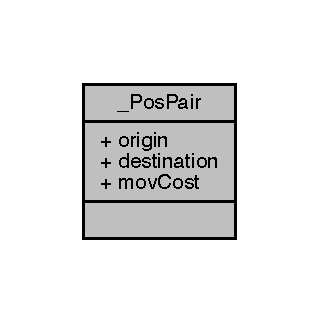
\includegraphics[width=153pt]{df/dfe/struct___pos_pair__coll__graph}
\end{center}
\end{figure}
\subsection*{Public Attributes}
\begin{DoxyCompactItemize}
\item 
int \mbox{\hyperlink{struct___pos_pair_a18ef19735976df84d1dda3185b844da0}{origin}}
\item 
int \mbox{\hyperlink{struct___pos_pair_a124d06bcfd8e7be752f9d32c0a7ce1bf}{destination}}
\item 
int \mbox{\hyperlink{struct___pos_pair_abf7f6970e1ace7a4f1cdc3179886e21d}{mov\+Cost}}
\end{DoxyCompactItemize}


\subsection{Member Data Documentation}
\mbox{\Hypertarget{struct___pos_pair_a124d06bcfd8e7be752f9d32c0a7ce1bf}\label{struct___pos_pair_a124d06bcfd8e7be752f9d32c0a7ce1bf}} 
\index{\+\_\+\+Pos\+Pair@{\+\_\+\+Pos\+Pair}!destination@{destination}}
\index{destination@{destination}!\+\_\+\+Pos\+Pair@{\+\_\+\+Pos\+Pair}}
\subsubsection{\texorpdfstring{destination}{destination}}
{\footnotesize\ttfamily int \+\_\+\+Pos\+Pair\+::destination}

\mbox{\Hypertarget{struct___pos_pair_abf7f6970e1ace7a4f1cdc3179886e21d}\label{struct___pos_pair_abf7f6970e1ace7a4f1cdc3179886e21d}} 
\index{\+\_\+\+Pos\+Pair@{\+\_\+\+Pos\+Pair}!mov\+Cost@{mov\+Cost}}
\index{mov\+Cost@{mov\+Cost}!\+\_\+\+Pos\+Pair@{\+\_\+\+Pos\+Pair}}
\subsubsection{\texorpdfstring{mov\+Cost}{movCost}}
{\footnotesize\ttfamily int \+\_\+\+Pos\+Pair\+::mov\+Cost}

\mbox{\Hypertarget{struct___pos_pair_a18ef19735976df84d1dda3185b844da0}\label{struct___pos_pair_a18ef19735976df84d1dda3185b844da0}} 
\index{\+\_\+\+Pos\+Pair@{\+\_\+\+Pos\+Pair}!origin@{origin}}
\index{origin@{origin}!\+\_\+\+Pos\+Pair@{\+\_\+\+Pos\+Pair}}
\subsubsection{\texorpdfstring{origin}{origin}}
{\footnotesize\ttfamily int \+\_\+\+Pos\+Pair\+::origin}



The documentation for this struct was generated from the following file\+:\begin{DoxyCompactItemize}
\item 
/\+Users/\+Afromullet/\+Documents/\+S\+F\+M\+L/\+Colony2/\+Colony/\mbox{\hyperlink{_pathfinding_8hpp}{Pathfinding.\+hpp}}\end{DoxyCompactItemize}

\hypertarget{class_anatomy___basic___d_f_s___visitor}{}\section{Anatomy\+\_\+\+Basic\+\_\+\+D\+F\+S\+\_\+\+Visitor Class Reference}
\label{class_anatomy___basic___d_f_s___visitor}\index{Anatomy\+\_\+\+Basic\+\_\+\+D\+F\+S\+\_\+\+Visitor@{Anatomy\+\_\+\+Basic\+\_\+\+D\+F\+S\+\_\+\+Visitor}}


{\ttfamily \#include $<$Body\+Graph\+Getters.\+hpp$>$}



Inheritance diagram for Anatomy\+\_\+\+Basic\+\_\+\+D\+F\+S\+\_\+\+Visitor\+:
\nopagebreak
\begin{figure}[H]
\begin{center}
\leavevmode
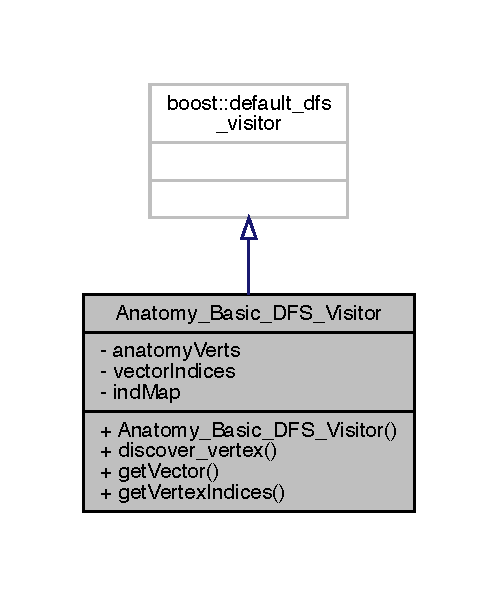
\includegraphics[width=239pt]{db/d04/class_anatomy___basic___d_f_s___visitor__inherit__graph}
\end{center}
\end{figure}


Collaboration diagram for Anatomy\+\_\+\+Basic\+\_\+\+D\+F\+S\+\_\+\+Visitor\+:
\nopagebreak
\begin{figure}[H]
\begin{center}
\leavevmode
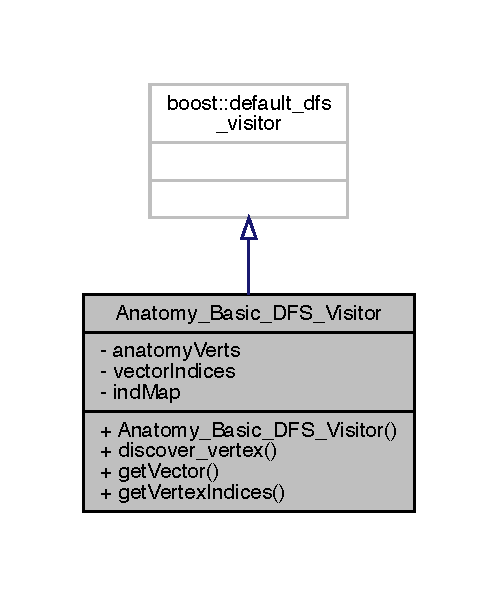
\includegraphics[width=239pt]{dc/d44/class_anatomy___basic___d_f_s___visitor__coll__graph}
\end{center}
\end{figure}
\subsection*{Public Member Functions}
\begin{DoxyCompactItemize}
\item 
\mbox{\hyperlink{class_anatomy___basic___d_f_s___visitor_ac0bad4df0cee8032fac56785830651b6}{Anatomy\+\_\+\+Basic\+\_\+\+D\+F\+S\+\_\+\+Visitor}} ()
\item 
void \mbox{\hyperlink{class_anatomy___basic___d_f_s___visitor_a718b8e46e3b31e6b046cc20dc1400054}{discover\+\_\+vertex}} (\mbox{\hyperlink{_body_graph_8hpp_aeb92fc7b3eed88cf25a4fc7b708a66cf}{Anatomy\+Vertex}} u, const \mbox{\hyperlink{_body_graph_8hpp_ab01b157c2e143191570b012d275fbf0d}{Anatomy\+Graph}} \&g) const
\item 
boost\+::shared\+\_\+ptr$<$ std\+::vector$<$ \mbox{\hyperlink{_body_graph_8hpp_aeb92fc7b3eed88cf25a4fc7b708a66cf}{Anatomy\+Vertex}} $>$ $>$ \mbox{\hyperlink{class_anatomy___basic___d_f_s___visitor_ad8e84fa450c5fb86f92d66adbeed782e}{get\+Vector}} ()
\item 
std\+::vector$<$ int $>$ \mbox{\hyperlink{class_anatomy___basic___d_f_s___visitor_aa4d4a9a684cd4ab15c965d3044530b76}{get\+Vertex\+Indices}} ()
\end{DoxyCompactItemize}
\subsection*{Private Attributes}
\begin{DoxyCompactItemize}
\item 
boost\+::shared\+\_\+ptr$<$ std\+::vector$<$ \mbox{\hyperlink{_body_graph_8hpp_aeb92fc7b3eed88cf25a4fc7b708a66cf}{Anatomy\+Vertex}} $>$ $>$ \mbox{\hyperlink{class_anatomy___basic___d_f_s___visitor_a0b28d945f501686b8037b49bb9ab75b2}{anatomy\+Verts}}
\item 
std\+::vector$<$ int $>$ \mbox{\hyperlink{class_anatomy___basic___d_f_s___visitor_a8e5871c69ac1e7ab736a2f31f3d35657}{vector\+Indices}}
\item 
\mbox{\hyperlink{_body_graph_8hpp_a9b727b123ee9682a6fc73a7785727450}{Anatomy\+Index\+Map}} \mbox{\hyperlink{class_anatomy___basic___d_f_s___visitor_a14840f6f0ba018b260db5d73e40fb326}{ind\+Map}}
\end{DoxyCompactItemize}


\subsection{Constructor \& Destructor Documentation}
\mbox{\Hypertarget{class_anatomy___basic___d_f_s___visitor_ac0bad4df0cee8032fac56785830651b6}\label{class_anatomy___basic___d_f_s___visitor_ac0bad4df0cee8032fac56785830651b6}} 
\index{Anatomy\+\_\+\+Basic\+\_\+\+D\+F\+S\+\_\+\+Visitor@{Anatomy\+\_\+\+Basic\+\_\+\+D\+F\+S\+\_\+\+Visitor}!Anatomy\+\_\+\+Basic\+\_\+\+D\+F\+S\+\_\+\+Visitor@{Anatomy\+\_\+\+Basic\+\_\+\+D\+F\+S\+\_\+\+Visitor}}
\index{Anatomy\+\_\+\+Basic\+\_\+\+D\+F\+S\+\_\+\+Visitor@{Anatomy\+\_\+\+Basic\+\_\+\+D\+F\+S\+\_\+\+Visitor}!Anatomy\+\_\+\+Basic\+\_\+\+D\+F\+S\+\_\+\+Visitor@{Anatomy\+\_\+\+Basic\+\_\+\+D\+F\+S\+\_\+\+Visitor}}
\subsubsection{\texorpdfstring{Anatomy\+\_\+\+Basic\+\_\+\+D\+F\+S\+\_\+\+Visitor()}{Anatomy\_Basic\_DFS\_Visitor()}}
{\footnotesize\ttfamily Anatomy\+\_\+\+Basic\+\_\+\+D\+F\+S\+\_\+\+Visitor\+::\+Anatomy\+\_\+\+Basic\+\_\+\+D\+F\+S\+\_\+\+Visitor (\begin{DoxyParamCaption}{ }\end{DoxyParamCaption})\hspace{0.3cm}{\ttfamily [inline]}}



\subsection{Member Function Documentation}
\mbox{\Hypertarget{class_anatomy___basic___d_f_s___visitor_a718b8e46e3b31e6b046cc20dc1400054}\label{class_anatomy___basic___d_f_s___visitor_a718b8e46e3b31e6b046cc20dc1400054}} 
\index{Anatomy\+\_\+\+Basic\+\_\+\+D\+F\+S\+\_\+\+Visitor@{Anatomy\+\_\+\+Basic\+\_\+\+D\+F\+S\+\_\+\+Visitor}!discover\+\_\+vertex@{discover\+\_\+vertex}}
\index{discover\+\_\+vertex@{discover\+\_\+vertex}!Anatomy\+\_\+\+Basic\+\_\+\+D\+F\+S\+\_\+\+Visitor@{Anatomy\+\_\+\+Basic\+\_\+\+D\+F\+S\+\_\+\+Visitor}}
\subsubsection{\texorpdfstring{discover\+\_\+vertex()}{discover\_vertex()}}
{\footnotesize\ttfamily void Anatomy\+\_\+\+Basic\+\_\+\+D\+F\+S\+\_\+\+Visitor\+::discover\+\_\+vertex (\begin{DoxyParamCaption}\item[{\mbox{\hyperlink{_body_graph_8hpp_aeb92fc7b3eed88cf25a4fc7b708a66cf}{Anatomy\+Vertex}}}]{u,  }\item[{const \mbox{\hyperlink{_body_graph_8hpp_ab01b157c2e143191570b012d275fbf0d}{Anatomy\+Graph}} \&}]{g }\end{DoxyParamCaption}) const\hspace{0.3cm}{\ttfamily [inline]}}

\mbox{\Hypertarget{class_anatomy___basic___d_f_s___visitor_ad8e84fa450c5fb86f92d66adbeed782e}\label{class_anatomy___basic___d_f_s___visitor_ad8e84fa450c5fb86f92d66adbeed782e}} 
\index{Anatomy\+\_\+\+Basic\+\_\+\+D\+F\+S\+\_\+\+Visitor@{Anatomy\+\_\+\+Basic\+\_\+\+D\+F\+S\+\_\+\+Visitor}!get\+Vector@{get\+Vector}}
\index{get\+Vector@{get\+Vector}!Anatomy\+\_\+\+Basic\+\_\+\+D\+F\+S\+\_\+\+Visitor@{Anatomy\+\_\+\+Basic\+\_\+\+D\+F\+S\+\_\+\+Visitor}}
\subsubsection{\texorpdfstring{get\+Vector()}{getVector()}}
{\footnotesize\ttfamily boost\+::shared\+\_\+ptr$<$std\+::vector$<$\mbox{\hyperlink{_body_graph_8hpp_aeb92fc7b3eed88cf25a4fc7b708a66cf}{Anatomy\+Vertex}}$>$ $>$ Anatomy\+\_\+\+Basic\+\_\+\+D\+F\+S\+\_\+\+Visitor\+::get\+Vector (\begin{DoxyParamCaption}{ }\end{DoxyParamCaption})\hspace{0.3cm}{\ttfamily [inline]}}

\mbox{\Hypertarget{class_anatomy___basic___d_f_s___visitor_aa4d4a9a684cd4ab15c965d3044530b76}\label{class_anatomy___basic___d_f_s___visitor_aa4d4a9a684cd4ab15c965d3044530b76}} 
\index{Anatomy\+\_\+\+Basic\+\_\+\+D\+F\+S\+\_\+\+Visitor@{Anatomy\+\_\+\+Basic\+\_\+\+D\+F\+S\+\_\+\+Visitor}!get\+Vertex\+Indices@{get\+Vertex\+Indices}}
\index{get\+Vertex\+Indices@{get\+Vertex\+Indices}!Anatomy\+\_\+\+Basic\+\_\+\+D\+F\+S\+\_\+\+Visitor@{Anatomy\+\_\+\+Basic\+\_\+\+D\+F\+S\+\_\+\+Visitor}}
\subsubsection{\texorpdfstring{get\+Vertex\+Indices()}{getVertexIndices()}}
{\footnotesize\ttfamily std\+::vector$<$int$>$ Anatomy\+\_\+\+Basic\+\_\+\+D\+F\+S\+\_\+\+Visitor\+::get\+Vertex\+Indices (\begin{DoxyParamCaption}{ }\end{DoxyParamCaption})\hspace{0.3cm}{\ttfamily [inline]}}

Here is the caller graph for this function\+:
\nopagebreak
\begin{figure}[H]
\begin{center}
\leavevmode
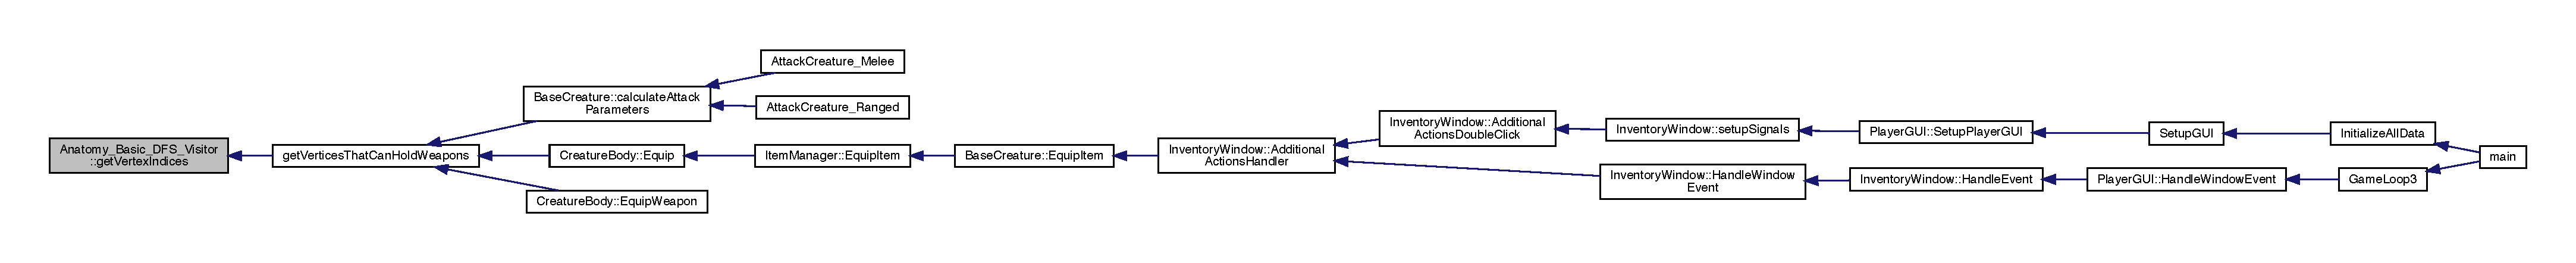
\includegraphics[width=350pt]{d5/db3/class_anatomy___basic___d_f_s___visitor_aa4d4a9a684cd4ab15c965d3044530b76_icgraph}
\end{center}
\end{figure}


\subsection{Member Data Documentation}
\mbox{\Hypertarget{class_anatomy___basic___d_f_s___visitor_a0b28d945f501686b8037b49bb9ab75b2}\label{class_anatomy___basic___d_f_s___visitor_a0b28d945f501686b8037b49bb9ab75b2}} 
\index{Anatomy\+\_\+\+Basic\+\_\+\+D\+F\+S\+\_\+\+Visitor@{Anatomy\+\_\+\+Basic\+\_\+\+D\+F\+S\+\_\+\+Visitor}!anatomy\+Verts@{anatomy\+Verts}}
\index{anatomy\+Verts@{anatomy\+Verts}!Anatomy\+\_\+\+Basic\+\_\+\+D\+F\+S\+\_\+\+Visitor@{Anatomy\+\_\+\+Basic\+\_\+\+D\+F\+S\+\_\+\+Visitor}}
\subsubsection{\texorpdfstring{anatomy\+Verts}{anatomyVerts}}
{\footnotesize\ttfamily boost\+::shared\+\_\+ptr$<$std\+::vector$<$\mbox{\hyperlink{_body_graph_8hpp_aeb92fc7b3eed88cf25a4fc7b708a66cf}{Anatomy\+Vertex}}$>$ $>$ Anatomy\+\_\+\+Basic\+\_\+\+D\+F\+S\+\_\+\+Visitor\+::anatomy\+Verts\hspace{0.3cm}{\ttfamily [private]}}

\mbox{\Hypertarget{class_anatomy___basic___d_f_s___visitor_a14840f6f0ba018b260db5d73e40fb326}\label{class_anatomy___basic___d_f_s___visitor_a14840f6f0ba018b260db5d73e40fb326}} 
\index{Anatomy\+\_\+\+Basic\+\_\+\+D\+F\+S\+\_\+\+Visitor@{Anatomy\+\_\+\+Basic\+\_\+\+D\+F\+S\+\_\+\+Visitor}!ind\+Map@{ind\+Map}}
\index{ind\+Map@{ind\+Map}!Anatomy\+\_\+\+Basic\+\_\+\+D\+F\+S\+\_\+\+Visitor@{Anatomy\+\_\+\+Basic\+\_\+\+D\+F\+S\+\_\+\+Visitor}}
\subsubsection{\texorpdfstring{ind\+Map}{indMap}}
{\footnotesize\ttfamily \mbox{\hyperlink{_body_graph_8hpp_a9b727b123ee9682a6fc73a7785727450}{Anatomy\+Index\+Map}} Anatomy\+\_\+\+Basic\+\_\+\+D\+F\+S\+\_\+\+Visitor\+::ind\+Map\hspace{0.3cm}{\ttfamily [private]}}

\mbox{\Hypertarget{class_anatomy___basic___d_f_s___visitor_a8e5871c69ac1e7ab736a2f31f3d35657}\label{class_anatomy___basic___d_f_s___visitor_a8e5871c69ac1e7ab736a2f31f3d35657}} 
\index{Anatomy\+\_\+\+Basic\+\_\+\+D\+F\+S\+\_\+\+Visitor@{Anatomy\+\_\+\+Basic\+\_\+\+D\+F\+S\+\_\+\+Visitor}!vector\+Indices@{vector\+Indices}}
\index{vector\+Indices@{vector\+Indices}!Anatomy\+\_\+\+Basic\+\_\+\+D\+F\+S\+\_\+\+Visitor@{Anatomy\+\_\+\+Basic\+\_\+\+D\+F\+S\+\_\+\+Visitor}}
\subsubsection{\texorpdfstring{vector\+Indices}{vectorIndices}}
{\footnotesize\ttfamily std\+::vector$<$int$>$ Anatomy\+\_\+\+Basic\+\_\+\+D\+F\+S\+\_\+\+Visitor\+::vector\+Indices\hspace{0.3cm}{\ttfamily [private]}}



The documentation for this class was generated from the following file\+:\begin{DoxyCompactItemize}
\item 
/\+Users/\+Afromullet/\+Documents/\+S\+F\+M\+L/\+Colony2/\+Colony/\+Creature/\+Body/\mbox{\hyperlink{_body_graph_getters_8hpp}{Body\+Graph\+Getters.\+hpp}}\end{DoxyCompactItemize}

\hypertarget{class_anatomy___d_f_s___section___visitor}{}\section{Anatomy\+\_\+\+D\+F\+S\+\_\+\+Section\+\_\+\+Visitor Class Reference}
\label{class_anatomy___d_f_s___section___visitor}\index{Anatomy\+\_\+\+D\+F\+S\+\_\+\+Section\+\_\+\+Visitor@{Anatomy\+\_\+\+D\+F\+S\+\_\+\+Section\+\_\+\+Visitor}}


{\ttfamily \#include $<$Body\+Graph\+Getters.\+hpp$>$}



Inheritance diagram for Anatomy\+\_\+\+D\+F\+S\+\_\+\+Section\+\_\+\+Visitor\+:
\nopagebreak
\begin{figure}[H]
\begin{center}
\leavevmode
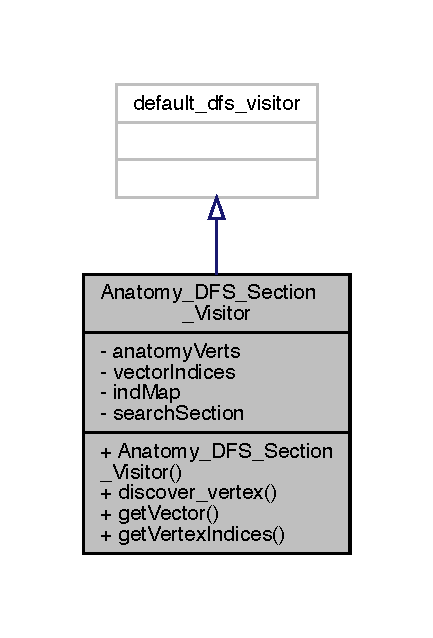
\includegraphics[width=208pt]{d5/d6f/class_anatomy___d_f_s___section___visitor__inherit__graph}
\end{center}
\end{figure}


Collaboration diagram for Anatomy\+\_\+\+D\+F\+S\+\_\+\+Section\+\_\+\+Visitor\+:
\nopagebreak
\begin{figure}[H]
\begin{center}
\leavevmode
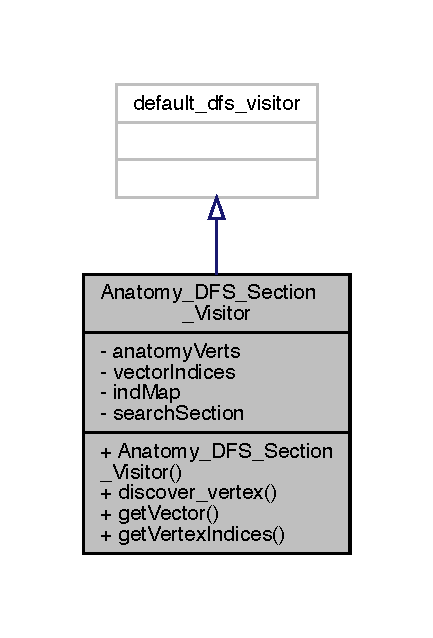
\includegraphics[width=208pt]{dd/d83/class_anatomy___d_f_s___section___visitor__coll__graph}
\end{center}
\end{figure}
\subsection*{Public Member Functions}
\begin{DoxyCompactItemize}
\item 
\mbox{\hyperlink{class_anatomy___d_f_s___section___visitor_a43610fbf5ffe403904d18fe32e568817}{Anatomy\+\_\+\+D\+F\+S\+\_\+\+Section\+\_\+\+Visitor}} (std\+::string section)
\item 
void \mbox{\hyperlink{class_anatomy___d_f_s___section___visitor_a97c0f08ebe41676b1effa6cd89c463cb}{discover\+\_\+vertex}} (\mbox{\hyperlink{_body_graph_8hpp_aeb92fc7b3eed88cf25a4fc7b708a66cf}{Anatomy\+Vertex}} u, const \mbox{\hyperlink{_body_graph_8hpp_ab01b157c2e143191570b012d275fbf0d}{Anatomy\+Graph}} \&g) const
\item 
boost\+::shared\+\_\+ptr$<$ std\+::vector$<$ \mbox{\hyperlink{_body_graph_8hpp_aeb92fc7b3eed88cf25a4fc7b708a66cf}{Anatomy\+Vertex}} $>$ $>$ \mbox{\hyperlink{class_anatomy___d_f_s___section___visitor_afc33d9738683a4e662545181ee596350}{get\+Vector}} ()
\item 
std\+::vector$<$ int $>$ \mbox{\hyperlink{class_anatomy___d_f_s___section___visitor_a9b7e0b16571acd04cde2b61b5094cb42}{get\+Vertex\+Indices}} ()
\end{DoxyCompactItemize}
\subsection*{Private Attributes}
\begin{DoxyCompactItemize}
\item 
boost\+::shared\+\_\+ptr$<$ std\+::vector$<$ \mbox{\hyperlink{_body_graph_8hpp_aeb92fc7b3eed88cf25a4fc7b708a66cf}{Anatomy\+Vertex}} $>$ $>$ \mbox{\hyperlink{class_anatomy___d_f_s___section___visitor_a8cfa2b3f70b1a3b54252d990d84e7842}{anatomy\+Verts}}
\item 
std\+::vector$<$ int $>$ \mbox{\hyperlink{class_anatomy___d_f_s___section___visitor_a12ea740c2f6405f5343ba2fdca3d180c}{vector\+Indices}}
\item 
\mbox{\hyperlink{_body_graph_8hpp_a9b727b123ee9682a6fc73a7785727450}{Anatomy\+Index\+Map}} \mbox{\hyperlink{class_anatomy___d_f_s___section___visitor_aa589aeb1afc570a76ff8bad92bcce25e}{ind\+Map}}
\item 
std\+::string \mbox{\hyperlink{class_anatomy___d_f_s___section___visitor_a99d83acb9c174dc61cfff9983f386f13}{search\+Section}}
\end{DoxyCompactItemize}


\subsection{Constructor \& Destructor Documentation}
\mbox{\Hypertarget{class_anatomy___d_f_s___section___visitor_a43610fbf5ffe403904d18fe32e568817}\label{class_anatomy___d_f_s___section___visitor_a43610fbf5ffe403904d18fe32e568817}} 
\index{Anatomy\+\_\+\+D\+F\+S\+\_\+\+Section\+\_\+\+Visitor@{Anatomy\+\_\+\+D\+F\+S\+\_\+\+Section\+\_\+\+Visitor}!Anatomy\+\_\+\+D\+F\+S\+\_\+\+Section\+\_\+\+Visitor@{Anatomy\+\_\+\+D\+F\+S\+\_\+\+Section\+\_\+\+Visitor}}
\index{Anatomy\+\_\+\+D\+F\+S\+\_\+\+Section\+\_\+\+Visitor@{Anatomy\+\_\+\+D\+F\+S\+\_\+\+Section\+\_\+\+Visitor}!Anatomy\+\_\+\+D\+F\+S\+\_\+\+Section\+\_\+\+Visitor@{Anatomy\+\_\+\+D\+F\+S\+\_\+\+Section\+\_\+\+Visitor}}
\subsubsection{\texorpdfstring{Anatomy\+\_\+\+D\+F\+S\+\_\+\+Section\+\_\+\+Visitor()}{Anatomy\_DFS\_Section\_Visitor()}}
{\footnotesize\ttfamily Anatomy\+\_\+\+D\+F\+S\+\_\+\+Section\+\_\+\+Visitor\+::\+Anatomy\+\_\+\+D\+F\+S\+\_\+\+Section\+\_\+\+Visitor (\begin{DoxyParamCaption}\item[{std\+::string}]{section }\end{DoxyParamCaption})\hspace{0.3cm}{\ttfamily [inline]}}



\subsection{Member Function Documentation}
\mbox{\Hypertarget{class_anatomy___d_f_s___section___visitor_a97c0f08ebe41676b1effa6cd89c463cb}\label{class_anatomy___d_f_s___section___visitor_a97c0f08ebe41676b1effa6cd89c463cb}} 
\index{Anatomy\+\_\+\+D\+F\+S\+\_\+\+Section\+\_\+\+Visitor@{Anatomy\+\_\+\+D\+F\+S\+\_\+\+Section\+\_\+\+Visitor}!discover\+\_\+vertex@{discover\+\_\+vertex}}
\index{discover\+\_\+vertex@{discover\+\_\+vertex}!Anatomy\+\_\+\+D\+F\+S\+\_\+\+Section\+\_\+\+Visitor@{Anatomy\+\_\+\+D\+F\+S\+\_\+\+Section\+\_\+\+Visitor}}
\subsubsection{\texorpdfstring{discover\+\_\+vertex()}{discover\_vertex()}}
{\footnotesize\ttfamily void Anatomy\+\_\+\+D\+F\+S\+\_\+\+Section\+\_\+\+Visitor\+::discover\+\_\+vertex (\begin{DoxyParamCaption}\item[{\mbox{\hyperlink{_body_graph_8hpp_aeb92fc7b3eed88cf25a4fc7b708a66cf}{Anatomy\+Vertex}}}]{u,  }\item[{const \mbox{\hyperlink{_body_graph_8hpp_ab01b157c2e143191570b012d275fbf0d}{Anatomy\+Graph}} \&}]{g }\end{DoxyParamCaption}) const\hspace{0.3cm}{\ttfamily [inline]}}

\mbox{\Hypertarget{class_anatomy___d_f_s___section___visitor_afc33d9738683a4e662545181ee596350}\label{class_anatomy___d_f_s___section___visitor_afc33d9738683a4e662545181ee596350}} 
\index{Anatomy\+\_\+\+D\+F\+S\+\_\+\+Section\+\_\+\+Visitor@{Anatomy\+\_\+\+D\+F\+S\+\_\+\+Section\+\_\+\+Visitor}!get\+Vector@{get\+Vector}}
\index{get\+Vector@{get\+Vector}!Anatomy\+\_\+\+D\+F\+S\+\_\+\+Section\+\_\+\+Visitor@{Anatomy\+\_\+\+D\+F\+S\+\_\+\+Section\+\_\+\+Visitor}}
\subsubsection{\texorpdfstring{get\+Vector()}{getVector()}}
{\footnotesize\ttfamily boost\+::shared\+\_\+ptr$<$std\+::vector$<$\mbox{\hyperlink{_body_graph_8hpp_aeb92fc7b3eed88cf25a4fc7b708a66cf}{Anatomy\+Vertex}}$>$ $>$ Anatomy\+\_\+\+D\+F\+S\+\_\+\+Section\+\_\+\+Visitor\+::get\+Vector (\begin{DoxyParamCaption}{ }\end{DoxyParamCaption})\hspace{0.3cm}{\ttfamily [inline]}}

\mbox{\Hypertarget{class_anatomy___d_f_s___section___visitor_a9b7e0b16571acd04cde2b61b5094cb42}\label{class_anatomy___d_f_s___section___visitor_a9b7e0b16571acd04cde2b61b5094cb42}} 
\index{Anatomy\+\_\+\+D\+F\+S\+\_\+\+Section\+\_\+\+Visitor@{Anatomy\+\_\+\+D\+F\+S\+\_\+\+Section\+\_\+\+Visitor}!get\+Vertex\+Indices@{get\+Vertex\+Indices}}
\index{get\+Vertex\+Indices@{get\+Vertex\+Indices}!Anatomy\+\_\+\+D\+F\+S\+\_\+\+Section\+\_\+\+Visitor@{Anatomy\+\_\+\+D\+F\+S\+\_\+\+Section\+\_\+\+Visitor}}
\subsubsection{\texorpdfstring{get\+Vertex\+Indices()}{getVertexIndices()}}
{\footnotesize\ttfamily std\+::vector$<$int$>$ Anatomy\+\_\+\+D\+F\+S\+\_\+\+Section\+\_\+\+Visitor\+::get\+Vertex\+Indices (\begin{DoxyParamCaption}{ }\end{DoxyParamCaption})\hspace{0.3cm}{\ttfamily [inline]}}

Here is the caller graph for this function\+:
\nopagebreak
\begin{figure}[H]
\begin{center}
\leavevmode
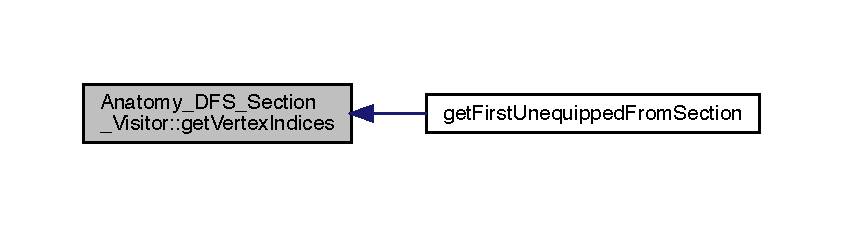
\includegraphics[width=350pt]{d4/da4/class_anatomy___d_f_s___section___visitor_a9b7e0b16571acd04cde2b61b5094cb42_icgraph}
\end{center}
\end{figure}


\subsection{Member Data Documentation}
\mbox{\Hypertarget{class_anatomy___d_f_s___section___visitor_a8cfa2b3f70b1a3b54252d990d84e7842}\label{class_anatomy___d_f_s___section___visitor_a8cfa2b3f70b1a3b54252d990d84e7842}} 
\index{Anatomy\+\_\+\+D\+F\+S\+\_\+\+Section\+\_\+\+Visitor@{Anatomy\+\_\+\+D\+F\+S\+\_\+\+Section\+\_\+\+Visitor}!anatomy\+Verts@{anatomy\+Verts}}
\index{anatomy\+Verts@{anatomy\+Verts}!Anatomy\+\_\+\+D\+F\+S\+\_\+\+Section\+\_\+\+Visitor@{Anatomy\+\_\+\+D\+F\+S\+\_\+\+Section\+\_\+\+Visitor}}
\subsubsection{\texorpdfstring{anatomy\+Verts}{anatomyVerts}}
{\footnotesize\ttfamily boost\+::shared\+\_\+ptr$<$std\+::vector$<$\mbox{\hyperlink{_body_graph_8hpp_aeb92fc7b3eed88cf25a4fc7b708a66cf}{Anatomy\+Vertex}}$>$ $>$ Anatomy\+\_\+\+D\+F\+S\+\_\+\+Section\+\_\+\+Visitor\+::anatomy\+Verts\hspace{0.3cm}{\ttfamily [private]}}

\mbox{\Hypertarget{class_anatomy___d_f_s___section___visitor_aa589aeb1afc570a76ff8bad92bcce25e}\label{class_anatomy___d_f_s___section___visitor_aa589aeb1afc570a76ff8bad92bcce25e}} 
\index{Anatomy\+\_\+\+D\+F\+S\+\_\+\+Section\+\_\+\+Visitor@{Anatomy\+\_\+\+D\+F\+S\+\_\+\+Section\+\_\+\+Visitor}!ind\+Map@{ind\+Map}}
\index{ind\+Map@{ind\+Map}!Anatomy\+\_\+\+D\+F\+S\+\_\+\+Section\+\_\+\+Visitor@{Anatomy\+\_\+\+D\+F\+S\+\_\+\+Section\+\_\+\+Visitor}}
\subsubsection{\texorpdfstring{ind\+Map}{indMap}}
{\footnotesize\ttfamily \mbox{\hyperlink{_body_graph_8hpp_a9b727b123ee9682a6fc73a7785727450}{Anatomy\+Index\+Map}} Anatomy\+\_\+\+D\+F\+S\+\_\+\+Section\+\_\+\+Visitor\+::ind\+Map\hspace{0.3cm}{\ttfamily [private]}}

\mbox{\Hypertarget{class_anatomy___d_f_s___section___visitor_a99d83acb9c174dc61cfff9983f386f13}\label{class_anatomy___d_f_s___section___visitor_a99d83acb9c174dc61cfff9983f386f13}} 
\index{Anatomy\+\_\+\+D\+F\+S\+\_\+\+Section\+\_\+\+Visitor@{Anatomy\+\_\+\+D\+F\+S\+\_\+\+Section\+\_\+\+Visitor}!search\+Section@{search\+Section}}
\index{search\+Section@{search\+Section}!Anatomy\+\_\+\+D\+F\+S\+\_\+\+Section\+\_\+\+Visitor@{Anatomy\+\_\+\+D\+F\+S\+\_\+\+Section\+\_\+\+Visitor}}
\subsubsection{\texorpdfstring{search\+Section}{searchSection}}
{\footnotesize\ttfamily std\+::string Anatomy\+\_\+\+D\+F\+S\+\_\+\+Section\+\_\+\+Visitor\+::search\+Section\hspace{0.3cm}{\ttfamily [private]}}

\mbox{\Hypertarget{class_anatomy___d_f_s___section___visitor_a12ea740c2f6405f5343ba2fdca3d180c}\label{class_anatomy___d_f_s___section___visitor_a12ea740c2f6405f5343ba2fdca3d180c}} 
\index{Anatomy\+\_\+\+D\+F\+S\+\_\+\+Section\+\_\+\+Visitor@{Anatomy\+\_\+\+D\+F\+S\+\_\+\+Section\+\_\+\+Visitor}!vector\+Indices@{vector\+Indices}}
\index{vector\+Indices@{vector\+Indices}!Anatomy\+\_\+\+D\+F\+S\+\_\+\+Section\+\_\+\+Visitor@{Anatomy\+\_\+\+D\+F\+S\+\_\+\+Section\+\_\+\+Visitor}}
\subsubsection{\texorpdfstring{vector\+Indices}{vectorIndices}}
{\footnotesize\ttfamily std\+::vector$<$int$>$ Anatomy\+\_\+\+D\+F\+S\+\_\+\+Section\+\_\+\+Visitor\+::vector\+Indices\hspace{0.3cm}{\ttfamily [private]}}



The documentation for this class was generated from the following file\+:\begin{DoxyCompactItemize}
\item 
/\+Users/\+Afromullet/\+Documents/\+S\+F\+M\+L/\+Colony2/\+Colony/\+Creature/\+Body/\mbox{\hyperlink{_body_graph_getters_8hpp}{Body\+Graph\+Getters.\+hpp}}\end{DoxyCompactItemize}

\hypertarget{struct_applied_force_effect}{}\section{Applied\+Force\+Effect Struct Reference}
\label{struct_applied_force_effect}\index{Applied\+Force\+Effect@{Applied\+Force\+Effect}}


{\ttfamily \#include $<$Material.\+hpp$>$}



Collaboration diagram for Applied\+Force\+Effect\+:
\nopagebreak
\begin{figure}[H]
\begin{center}
\leavevmode
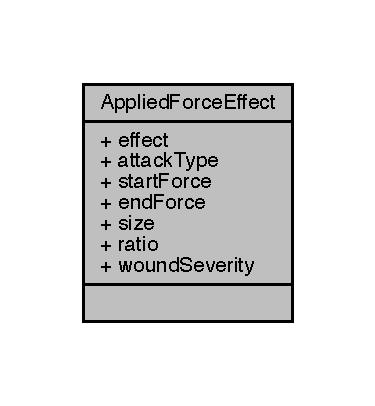
\includegraphics[width=180pt]{struct_applied_force_effect__coll__graph}
\end{center}
\end{figure}
\subsection*{Public Attributes}
\begin{DoxyCompactItemize}
\item 
\mbox{\hyperlink{_material_8hpp_a666cff003097e3165d55b4b1c269a2e6}{en\+Material\+Effect}} \mbox{\hyperlink{struct_applied_force_effect_aa78faf3596c6557107dcd902b0397811}{effect}}
\item 
\mbox{\hyperlink{_enum_types_8hpp_a904b2f9c8f3951116c343784c59d6afe}{Attack\+Type}} \mbox{\hyperlink{struct_applied_force_effect_abf55a5ab31b65c1b6781a863ef7c3b75}{attack\+Type}}
\item 
float \mbox{\hyperlink{struct_applied_force_effect_a041935c570639c9f1f87e34e114f204e}{start\+Force}}
\item 
float \mbox{\hyperlink{struct_applied_force_effect_a59d301bbc9070156ed39cf672b2724bf}{end\+Force}}
\item 
float \mbox{\hyperlink{struct_applied_force_effect_aa50dc7f47801c66dc9df54d8fb281cf0}{size}}
\item 
float \mbox{\hyperlink{struct_applied_force_effect_a01ede7323a840f3f44bc9200e9b8e8f9}{ratio}}
\item 
\mbox{\hyperlink{_enum_types_8hpp_a295be2e2d0f307f31ad832b24a7736c6}{Wound\+Severity}} \mbox{\hyperlink{struct_applied_force_effect_a5aa8b89ec11b997955d4160b3fb671ec}{wound\+Severity}}
\end{DoxyCompactItemize}


\subsection{Member Data Documentation}
\mbox{\Hypertarget{struct_applied_force_effect_abf55a5ab31b65c1b6781a863ef7c3b75}\label{struct_applied_force_effect_abf55a5ab31b65c1b6781a863ef7c3b75}} 
\index{Applied\+Force\+Effect@{Applied\+Force\+Effect}!attack\+Type@{attack\+Type}}
\index{attack\+Type@{attack\+Type}!Applied\+Force\+Effect@{Applied\+Force\+Effect}}
\subsubsection{\texorpdfstring{attack\+Type}{attackType}}
{\footnotesize\ttfamily \mbox{\hyperlink{_enum_types_8hpp_a904b2f9c8f3951116c343784c59d6afe}{Attack\+Type}} Applied\+Force\+Effect\+::attack\+Type}

\mbox{\Hypertarget{struct_applied_force_effect_aa78faf3596c6557107dcd902b0397811}\label{struct_applied_force_effect_aa78faf3596c6557107dcd902b0397811}} 
\index{Applied\+Force\+Effect@{Applied\+Force\+Effect}!effect@{effect}}
\index{effect@{effect}!Applied\+Force\+Effect@{Applied\+Force\+Effect}}
\subsubsection{\texorpdfstring{effect}{effect}}
{\footnotesize\ttfamily \mbox{\hyperlink{_material_8hpp_a666cff003097e3165d55b4b1c269a2e6}{en\+Material\+Effect}} Applied\+Force\+Effect\+::effect}

\mbox{\Hypertarget{struct_applied_force_effect_a59d301bbc9070156ed39cf672b2724bf}\label{struct_applied_force_effect_a59d301bbc9070156ed39cf672b2724bf}} 
\index{Applied\+Force\+Effect@{Applied\+Force\+Effect}!end\+Force@{end\+Force}}
\index{end\+Force@{end\+Force}!Applied\+Force\+Effect@{Applied\+Force\+Effect}}
\subsubsection{\texorpdfstring{end\+Force}{endForce}}
{\footnotesize\ttfamily float Applied\+Force\+Effect\+::end\+Force}

\mbox{\Hypertarget{struct_applied_force_effect_a01ede7323a840f3f44bc9200e9b8e8f9}\label{struct_applied_force_effect_a01ede7323a840f3f44bc9200e9b8e8f9}} 
\index{Applied\+Force\+Effect@{Applied\+Force\+Effect}!ratio@{ratio}}
\index{ratio@{ratio}!Applied\+Force\+Effect@{Applied\+Force\+Effect}}
\subsubsection{\texorpdfstring{ratio}{ratio}}
{\footnotesize\ttfamily float Applied\+Force\+Effect\+::ratio}

\mbox{\Hypertarget{struct_applied_force_effect_aa50dc7f47801c66dc9df54d8fb281cf0}\label{struct_applied_force_effect_aa50dc7f47801c66dc9df54d8fb281cf0}} 
\index{Applied\+Force\+Effect@{Applied\+Force\+Effect}!size@{size}}
\index{size@{size}!Applied\+Force\+Effect@{Applied\+Force\+Effect}}
\subsubsection{\texorpdfstring{size}{size}}
{\footnotesize\ttfamily float Applied\+Force\+Effect\+::size}

\mbox{\Hypertarget{struct_applied_force_effect_a041935c570639c9f1f87e34e114f204e}\label{struct_applied_force_effect_a041935c570639c9f1f87e34e114f204e}} 
\index{Applied\+Force\+Effect@{Applied\+Force\+Effect}!start\+Force@{start\+Force}}
\index{start\+Force@{start\+Force}!Applied\+Force\+Effect@{Applied\+Force\+Effect}}
\subsubsection{\texorpdfstring{start\+Force}{startForce}}
{\footnotesize\ttfamily float Applied\+Force\+Effect\+::start\+Force}

\mbox{\Hypertarget{struct_applied_force_effect_a5aa8b89ec11b997955d4160b3fb671ec}\label{struct_applied_force_effect_a5aa8b89ec11b997955d4160b3fb671ec}} 
\index{Applied\+Force\+Effect@{Applied\+Force\+Effect}!wound\+Severity@{wound\+Severity}}
\index{wound\+Severity@{wound\+Severity}!Applied\+Force\+Effect@{Applied\+Force\+Effect}}
\subsubsection{\texorpdfstring{wound\+Severity}{woundSeverity}}
{\footnotesize\ttfamily \mbox{\hyperlink{_enum_types_8hpp_a295be2e2d0f307f31ad832b24a7736c6}{Wound\+Severity}} Applied\+Force\+Effect\+::wound\+Severity}



The documentation for this struct was generated from the following file\+:\begin{DoxyCompactItemize}
\item 
/\+Users/\+Afromullet/\+Documents/\+S\+F\+M\+L/\+Colony2/\+Colony/\+Data/\mbox{\hyperlink{_material_8hpp}{Material.\+hpp}}\end{DoxyCompactItemize}

\hypertarget{class_armor}{}\section{Armor Class Reference}
\label{class_armor}\index{Armor@{Armor}}


{\ttfamily \#include $<$Armor.\+hpp$>$}



Inheritance diagram for Armor\+:
\nopagebreak
\begin{figure}[H]
\begin{center}
\leavevmode
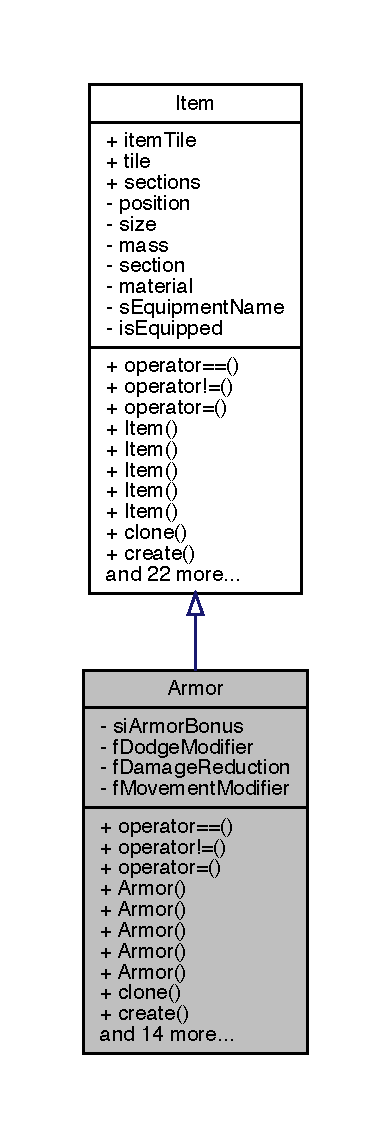
\includegraphics[height=550pt]{db/d06/class_armor__inherit__graph}
\end{center}
\end{figure}


Collaboration diagram for Armor\+:
\nopagebreak
\begin{figure}[H]
\begin{center}
\leavevmode
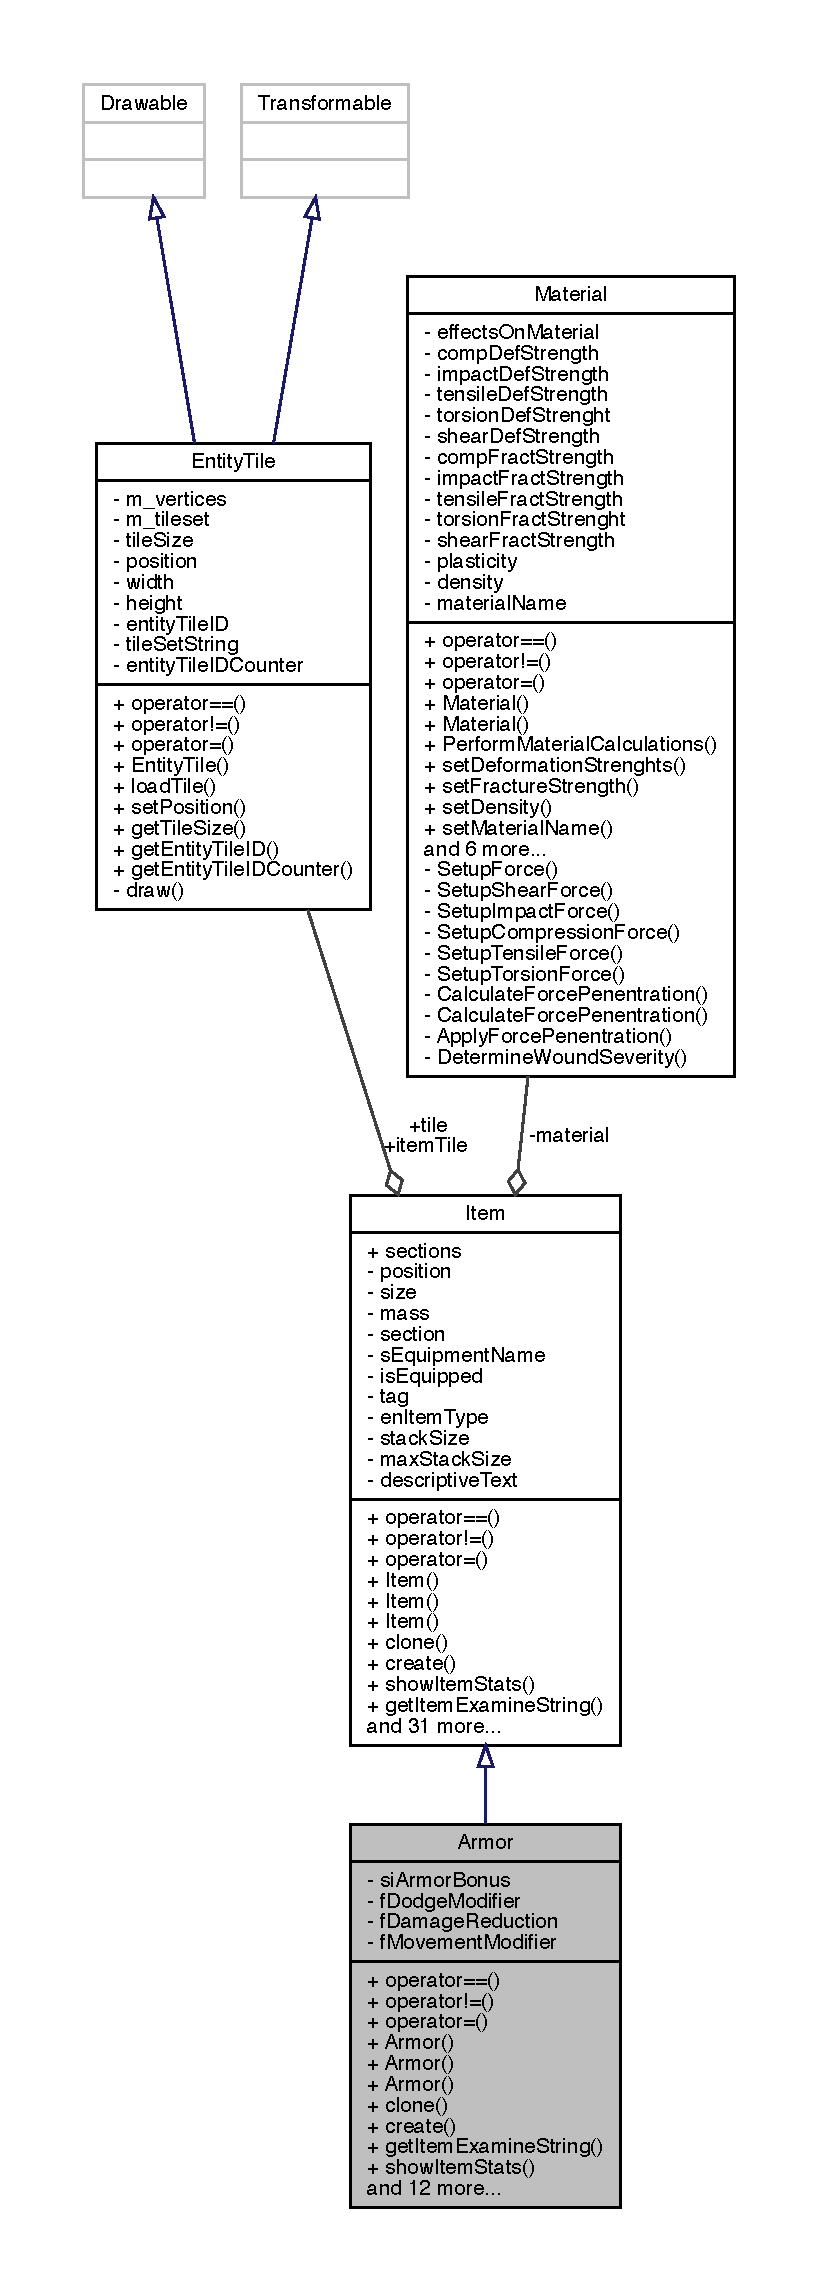
\includegraphics[height=550pt]{d0/d90/class_armor__coll__graph}
\end{center}
\end{figure}
\subsection*{Public Member Functions}
\begin{DoxyCompactItemize}
\item 
bool \mbox{\hyperlink{class_armor_a400f558650400d25fc5fc3031a455c46}{operator==}} (const \mbox{\hyperlink{class_armor}{Armor}} \&other) const
\item 
bool \mbox{\hyperlink{class_armor_a912e1ad6bfe7509c66c2c4966cf5188c}{operator!=}} (const \mbox{\hyperlink{class_armor}{Armor}} \&other) const
\item 
void \mbox{\hyperlink{class_armor_ad706d994c7d3a3ea4d7c1728faccc0aa}{operator=}} (const \mbox{\hyperlink{class_armor}{Armor}} \&other)
\item 
\mbox{\hyperlink{class_armor_a4a33d37eb11165792cce7035dfb2ff93}{Armor}} (\mbox{\hyperlink{class_material}{Material}} \+\_\+material, std\+::string \+\_\+s\+Equipment\+Name, short int \+\_\+si\+Armor\+Bonus, float \+\_\+f\+Dodge\+Modifier, float \+\_\+f\+Damage\+Reduction, float \+\_\+f\+Movement\+Modifier)
\item 
\mbox{\hyperlink{class_armor_a40d54a621183a93edaecb2cd4e83c800}{Armor}} (const \mbox{\hyperlink{class_armor}{Armor}} \&other)
\item 
\mbox{\hyperlink{class_armor_a23323e95bbeb488eb6fe54cbd83d49a2}{Armor}} ()
\item 
\mbox{\hyperlink{class_armor}{Armor}} $\ast$ \mbox{\hyperlink{class_armor_aac8aec108de9a8a45bada1534c0f23b7}{clone}} () const
\item 
\mbox{\hyperlink{class_armor}{Armor}} $\ast$ \mbox{\hyperlink{class_armor_a21de0acaa6ecdb6f5937166b83da9b01}{create}} () const
\item 
std\+::string \mbox{\hyperlink{class_armor_a731bb4d1fe53070f30a336db82fada2c}{get\+Item\+Examine\+String}} () const
\item 
void \mbox{\hyperlink{class_armor_a4fe1507d7aaf280a18e19f51a6f8c42d}{show\+Item\+Stats}} () const
\item 
void \mbox{\hyperlink{class_armor_a697e23862a5a6bb32fc5b1b143d61f58}{Equip\+Item}} (\mbox{\hyperlink{class_body_part}{Body\+Part}} \&bp)
\item 
void \mbox{\hyperlink{class_armor_a248a63d0d2801a10d6a4039f60b6a0c7}{Print\+Armor\+Statistics}} ()
\item 
void \mbox{\hyperlink{class_armor_a008a9def7f07c141c87771937d856616}{Add\+To\+Item\+Manager}} (\mbox{\hyperlink{class_item_manager}{Item\+Manager}} \&manager)
\item 
short int \mbox{\hyperlink{class_armor_a72b3d5c0294e80243ed8c96dbc35ccc7}{si\+Get\+Armor\+Bonus}} () const
\item 
float \mbox{\hyperlink{class_armor_a2eab88550e74345eef13e2a279a2f995}{f\+Get\+Dodge\+Modifier}} () const
\item 
float \mbox{\hyperlink{class_armor_a2ac47305b38298494fae82c69c935fba}{f\+Get\+Damage\+Reduction}} () const
\item 
float \mbox{\hyperlink{class_armor_a788fee5745a82a7ffc587aa4938200dc}{f\+Get\+Movement\+Modifier}} () const
\item 
void \mbox{\hyperlink{class_armor_a14c15f72741f2a3dec28c746b3678c20}{set\+Armor\+Bonus}} (short int value)
\item 
void \mbox{\hyperlink{class_armor_ab48309e3f16d226d56af617c65350698}{set\+Dodge\+Modifier}} (float value)
\item 
void \mbox{\hyperlink{class_armor_a08f926ae8438bae04058c22b098c6fcf}{set\+Damage\+Reduction}} (float value)
\item 
void \mbox{\hyperlink{class_armor_a99475fc688add41f89b7fef160534e33}{set\+Movement\+Modifier}} (float value)
\item 
void \mbox{\hyperlink{class_armor_a1710521cbba1bf9328e969cbbc8cdbf3}{set\+Material}} (\mbox{\hyperlink{class_material}{Material}} value)
\end{DoxyCompactItemize}
\subsection*{Private Attributes}
\begin{DoxyCompactItemize}
\item 
short int \mbox{\hyperlink{class_armor_a2ebccb72313c650ec1b8bafec4e82dc2}{si\+Armor\+Bonus}}
\item 
float \mbox{\hyperlink{class_armor_aed2f98ba9acefdb67ac75104c55ea266}{f\+Dodge\+Modifier}}
\item 
float \mbox{\hyperlink{class_armor_acc29c5818b294aaaa11d8d1621b7dd19}{f\+Damage\+Reduction}}
\item 
float \mbox{\hyperlink{class_armor_aa71e430d9308cfe64b5168014c063722}{f\+Movement\+Modifier}}
\end{DoxyCompactItemize}
\subsection*{Friends}
\begin{DoxyCompactItemize}
\item 
class \mbox{\hyperlink{class_armor_aad85754f188b769ff61150eaf36106c4}{Item}}
\end{DoxyCompactItemize}
\subsection*{Additional Inherited Members}


\subsection{Constructor \& Destructor Documentation}
\mbox{\Hypertarget{class_armor_a4a33d37eb11165792cce7035dfb2ff93}\label{class_armor_a4a33d37eb11165792cce7035dfb2ff93}} 
\index{Armor@{Armor}!Armor@{Armor}}
\index{Armor@{Armor}!Armor@{Armor}}
\subsubsection{\texorpdfstring{Armor()}{Armor()}\hspace{0.1cm}{\footnotesize\ttfamily [1/3]}}
{\footnotesize\ttfamily Armor\+::\+Armor (\begin{DoxyParamCaption}\item[{\mbox{\hyperlink{class_material}{Material}}}]{\+\_\+material,  }\item[{std\+::string}]{\+\_\+s\+Equipment\+Name,  }\item[{short int}]{\+\_\+si\+Armor\+Bonus,  }\item[{float}]{\+\_\+f\+Dodge\+Modifier,  }\item[{float}]{\+\_\+f\+Damage\+Reduction,  }\item[{float}]{\+\_\+f\+Movement\+Modifier }\end{DoxyParamCaption})}

\mbox{\Hypertarget{class_armor_a40d54a621183a93edaecb2cd4e83c800}\label{class_armor_a40d54a621183a93edaecb2cd4e83c800}} 
\index{Armor@{Armor}!Armor@{Armor}}
\index{Armor@{Armor}!Armor@{Armor}}
\subsubsection{\texorpdfstring{Armor()}{Armor()}\hspace{0.1cm}{\footnotesize\ttfamily [2/3]}}
{\footnotesize\ttfamily Armor\+::\+Armor (\begin{DoxyParamCaption}\item[{const \mbox{\hyperlink{class_armor}{Armor}} \&}]{other }\end{DoxyParamCaption})}

\mbox{\Hypertarget{class_armor_a23323e95bbeb488eb6fe54cbd83d49a2}\label{class_armor_a23323e95bbeb488eb6fe54cbd83d49a2}} 
\index{Armor@{Armor}!Armor@{Armor}}
\index{Armor@{Armor}!Armor@{Armor}}
\subsubsection{\texorpdfstring{Armor()}{Armor()}\hspace{0.1cm}{\footnotesize\ttfamily [3/3]}}
{\footnotesize\ttfamily Armor\+::\+Armor (\begin{DoxyParamCaption}{ }\end{DoxyParamCaption})}

Here is the caller graph for this function\+:
\nopagebreak
\begin{figure}[H]
\begin{center}
\leavevmode
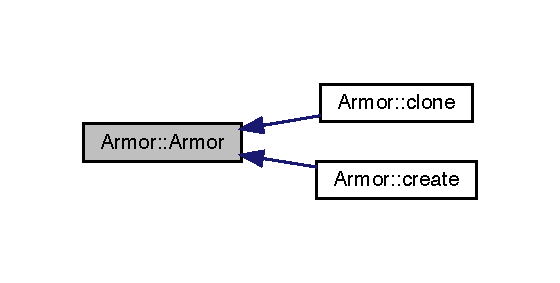
\includegraphics[width=269pt]{d9/d76/class_armor_a23323e95bbeb488eb6fe54cbd83d49a2_icgraph}
\end{center}
\end{figure}


\subsection{Member Function Documentation}
\mbox{\Hypertarget{class_armor_a008a9def7f07c141c87771937d856616}\label{class_armor_a008a9def7f07c141c87771937d856616}} 
\index{Armor@{Armor}!Add\+To\+Item\+Manager@{Add\+To\+Item\+Manager}}
\index{Add\+To\+Item\+Manager@{Add\+To\+Item\+Manager}!Armor@{Armor}}
\subsubsection{\texorpdfstring{Add\+To\+Item\+Manager()}{AddToItemManager()}}
{\footnotesize\ttfamily void Armor\+::\+Add\+To\+Item\+Manager (\begin{DoxyParamCaption}\item[{\mbox{\hyperlink{class_item_manager}{Item\+Manager}} \&}]{manager }\end{DoxyParamCaption})\hspace{0.3cm}{\ttfamily [virtual]}}



Implements \mbox{\hyperlink{class_item_ae534538f3e77078f804acc742ef68521}{Item}}.

Here is the call graph for this function\+:
\nopagebreak
\begin{figure}[H]
\begin{center}
\leavevmode
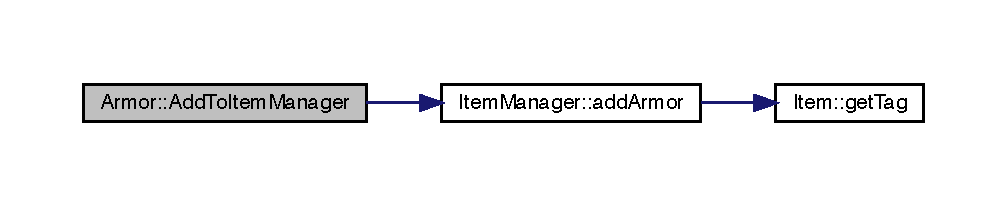
\includegraphics[width=350pt]{d9/d76/class_armor_a008a9def7f07c141c87771937d856616_cgraph}
\end{center}
\end{figure}
\mbox{\Hypertarget{class_armor_aac8aec108de9a8a45bada1534c0f23b7}\label{class_armor_aac8aec108de9a8a45bada1534c0f23b7}} 
\index{Armor@{Armor}!clone@{clone}}
\index{clone@{clone}!Armor@{Armor}}
\subsubsection{\texorpdfstring{clone()}{clone()}}
{\footnotesize\ttfamily \mbox{\hyperlink{class_armor}{Armor}}$\ast$ Armor\+::clone (\begin{DoxyParamCaption}{ }\end{DoxyParamCaption}) const\hspace{0.3cm}{\ttfamily [inline]}, {\ttfamily [virtual]}}



Implements \mbox{\hyperlink{class_item_a6d963581e2caad2e08979683a827f39f}{Item}}.

Here is the call graph for this function\+:
\nopagebreak
\begin{figure}[H]
\begin{center}
\leavevmode
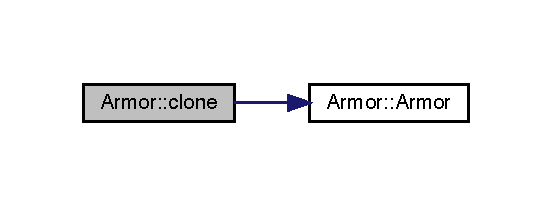
\includegraphics[width=265pt]{d9/d76/class_armor_aac8aec108de9a8a45bada1534c0f23b7_cgraph}
\end{center}
\end{figure}
\mbox{\Hypertarget{class_armor_a21de0acaa6ecdb6f5937166b83da9b01}\label{class_armor_a21de0acaa6ecdb6f5937166b83da9b01}} 
\index{Armor@{Armor}!create@{create}}
\index{create@{create}!Armor@{Armor}}
\subsubsection{\texorpdfstring{create()}{create()}}
{\footnotesize\ttfamily \mbox{\hyperlink{class_armor}{Armor}}$\ast$ Armor\+::create (\begin{DoxyParamCaption}{ }\end{DoxyParamCaption}) const\hspace{0.3cm}{\ttfamily [inline]}, {\ttfamily [virtual]}}



Implements \mbox{\hyperlink{class_item_a17b3fa0cef44ada961e0d3c65e1de864}{Item}}.

Here is the call graph for this function\+:
\nopagebreak
\begin{figure}[H]
\begin{center}
\leavevmode
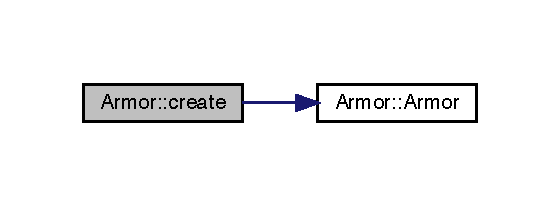
\includegraphics[width=269pt]{d9/d76/class_armor_a21de0acaa6ecdb6f5937166b83da9b01_cgraph}
\end{center}
\end{figure}
\mbox{\Hypertarget{class_armor_a697e23862a5a6bb32fc5b1b143d61f58}\label{class_armor_a697e23862a5a6bb32fc5b1b143d61f58}} 
\index{Armor@{Armor}!Equip\+Item@{Equip\+Item}}
\index{Equip\+Item@{Equip\+Item}!Armor@{Armor}}
\subsubsection{\texorpdfstring{Equip\+Item()}{EquipItem()}}
{\footnotesize\ttfamily void Armor\+::\+Equip\+Item (\begin{DoxyParamCaption}\item[{\mbox{\hyperlink{class_body_part}{Body\+Part}} \&}]{bp }\end{DoxyParamCaption})\hspace{0.3cm}{\ttfamily [virtual]}}



Implements \mbox{\hyperlink{class_item_af4b9caf8fcfc22bbde13bf6c3505b35c}{Item}}.

Here is the call graph for this function\+:
\nopagebreak
\begin{figure}[H]
\begin{center}
\leavevmode
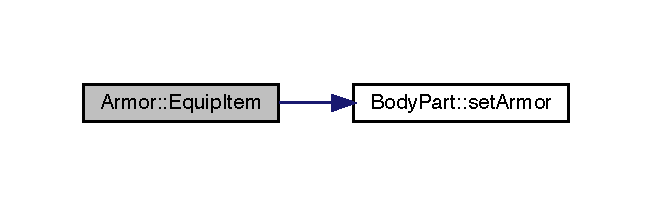
\includegraphics[width=313pt]{d9/d76/class_armor_a697e23862a5a6bb32fc5b1b143d61f58_cgraph}
\end{center}
\end{figure}
Here is the caller graph for this function\+:
\nopagebreak
\begin{figure}[H]
\begin{center}
\leavevmode
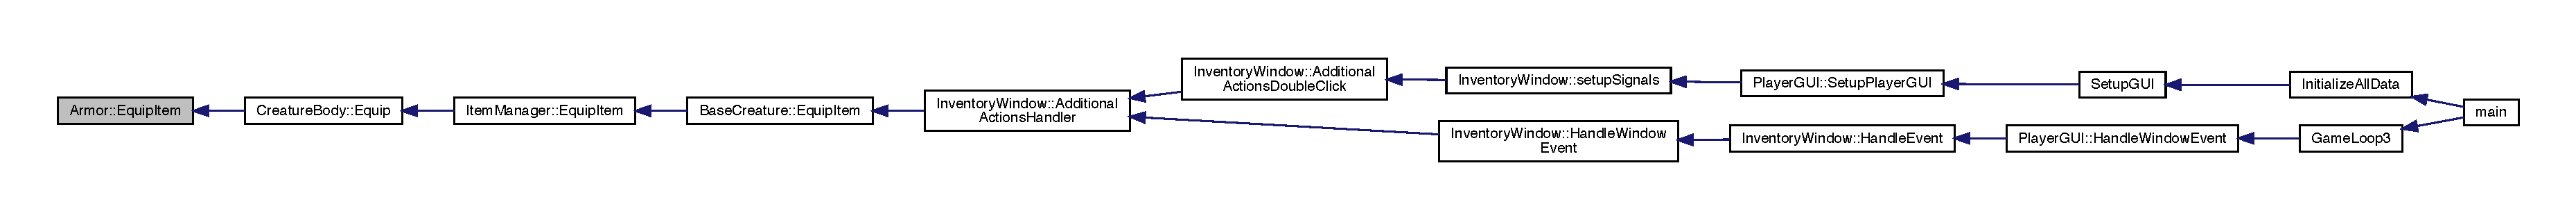
\includegraphics[width=350pt]{d9/d76/class_armor_a697e23862a5a6bb32fc5b1b143d61f58_icgraph}
\end{center}
\end{figure}
\mbox{\Hypertarget{class_armor_a2ac47305b38298494fae82c69c935fba}\label{class_armor_a2ac47305b38298494fae82c69c935fba}} 
\index{Armor@{Armor}!f\+Get\+Damage\+Reduction@{f\+Get\+Damage\+Reduction}}
\index{f\+Get\+Damage\+Reduction@{f\+Get\+Damage\+Reduction}!Armor@{Armor}}
\subsubsection{\texorpdfstring{f\+Get\+Damage\+Reduction()}{fGetDamageReduction()}}
{\footnotesize\ttfamily float Armor\+::f\+Get\+Damage\+Reduction (\begin{DoxyParamCaption}{ }\end{DoxyParamCaption}) const}

\mbox{\Hypertarget{class_armor_a2eab88550e74345eef13e2a279a2f995}\label{class_armor_a2eab88550e74345eef13e2a279a2f995}} 
\index{Armor@{Armor}!f\+Get\+Dodge\+Modifier@{f\+Get\+Dodge\+Modifier}}
\index{f\+Get\+Dodge\+Modifier@{f\+Get\+Dodge\+Modifier}!Armor@{Armor}}
\subsubsection{\texorpdfstring{f\+Get\+Dodge\+Modifier()}{fGetDodgeModifier()}}
{\footnotesize\ttfamily float Armor\+::f\+Get\+Dodge\+Modifier (\begin{DoxyParamCaption}{ }\end{DoxyParamCaption}) const}

\mbox{\Hypertarget{class_armor_a788fee5745a82a7ffc587aa4938200dc}\label{class_armor_a788fee5745a82a7ffc587aa4938200dc}} 
\index{Armor@{Armor}!f\+Get\+Movement\+Modifier@{f\+Get\+Movement\+Modifier}}
\index{f\+Get\+Movement\+Modifier@{f\+Get\+Movement\+Modifier}!Armor@{Armor}}
\subsubsection{\texorpdfstring{f\+Get\+Movement\+Modifier()}{fGetMovementModifier()}}
{\footnotesize\ttfamily float Armor\+::f\+Get\+Movement\+Modifier (\begin{DoxyParamCaption}{ }\end{DoxyParamCaption}) const}

\mbox{\Hypertarget{class_armor_a731bb4d1fe53070f30a336db82fada2c}\label{class_armor_a731bb4d1fe53070f30a336db82fada2c}} 
\index{Armor@{Armor}!get\+Item\+Examine\+String@{get\+Item\+Examine\+String}}
\index{get\+Item\+Examine\+String@{get\+Item\+Examine\+String}!Armor@{Armor}}
\subsubsection{\texorpdfstring{get\+Item\+Examine\+String()}{getItemExamineString()}}
{\footnotesize\ttfamily std\+::string Armor\+::get\+Item\+Examine\+String (\begin{DoxyParamCaption}{ }\end{DoxyParamCaption}) const\hspace{0.3cm}{\ttfamily [virtual]}}



Implements \mbox{\hyperlink{class_item_a00e06647e1adeb62f2d95044476126ac}{Item}}.

\mbox{\Hypertarget{class_armor_a912e1ad6bfe7509c66c2c4966cf5188c}\label{class_armor_a912e1ad6bfe7509c66c2c4966cf5188c}} 
\index{Armor@{Armor}!operator"!=@{operator"!=}}
\index{operator"!=@{operator"!=}!Armor@{Armor}}
\subsubsection{\texorpdfstring{operator"!=()}{operator!=()}}
{\footnotesize\ttfamily bool Armor\+::operator!= (\begin{DoxyParamCaption}\item[{const \mbox{\hyperlink{class_armor}{Armor}} \&}]{other }\end{DoxyParamCaption}) const}

\mbox{\Hypertarget{class_armor_ad706d994c7d3a3ea4d7c1728faccc0aa}\label{class_armor_ad706d994c7d3a3ea4d7c1728faccc0aa}} 
\index{Armor@{Armor}!operator=@{operator=}}
\index{operator=@{operator=}!Armor@{Armor}}
\subsubsection{\texorpdfstring{operator=()}{operator=()}}
{\footnotesize\ttfamily void Armor\+::operator= (\begin{DoxyParamCaption}\item[{const \mbox{\hyperlink{class_armor}{Armor}} \&}]{other }\end{DoxyParamCaption})}

\mbox{\Hypertarget{class_armor_a400f558650400d25fc5fc3031a455c46}\label{class_armor_a400f558650400d25fc5fc3031a455c46}} 
\index{Armor@{Armor}!operator==@{operator==}}
\index{operator==@{operator==}!Armor@{Armor}}
\subsubsection{\texorpdfstring{operator==()}{operator==()}}
{\footnotesize\ttfamily bool Armor\+::operator== (\begin{DoxyParamCaption}\item[{const \mbox{\hyperlink{class_armor}{Armor}} \&}]{other }\end{DoxyParamCaption}) const}

\mbox{\Hypertarget{class_armor_a248a63d0d2801a10d6a4039f60b6a0c7}\label{class_armor_a248a63d0d2801a10d6a4039f60b6a0c7}} 
\index{Armor@{Armor}!Print\+Armor\+Statistics@{Print\+Armor\+Statistics}}
\index{Print\+Armor\+Statistics@{Print\+Armor\+Statistics}!Armor@{Armor}}
\subsubsection{\texorpdfstring{Print\+Armor\+Statistics()}{PrintArmorStatistics()}}
{\footnotesize\ttfamily void Armor\+::\+Print\+Armor\+Statistics (\begin{DoxyParamCaption}{ }\end{DoxyParamCaption})}

\mbox{\Hypertarget{class_armor_a14c15f72741f2a3dec28c746b3678c20}\label{class_armor_a14c15f72741f2a3dec28c746b3678c20}} 
\index{Armor@{Armor}!set\+Armor\+Bonus@{set\+Armor\+Bonus}}
\index{set\+Armor\+Bonus@{set\+Armor\+Bonus}!Armor@{Armor}}
\subsubsection{\texorpdfstring{set\+Armor\+Bonus()}{setArmorBonus()}}
{\footnotesize\ttfamily void Armor\+::set\+Armor\+Bonus (\begin{DoxyParamCaption}\item[{short int}]{value }\end{DoxyParamCaption})}

Here is the caller graph for this function\+:
\nopagebreak
\begin{figure}[H]
\begin{center}
\leavevmode
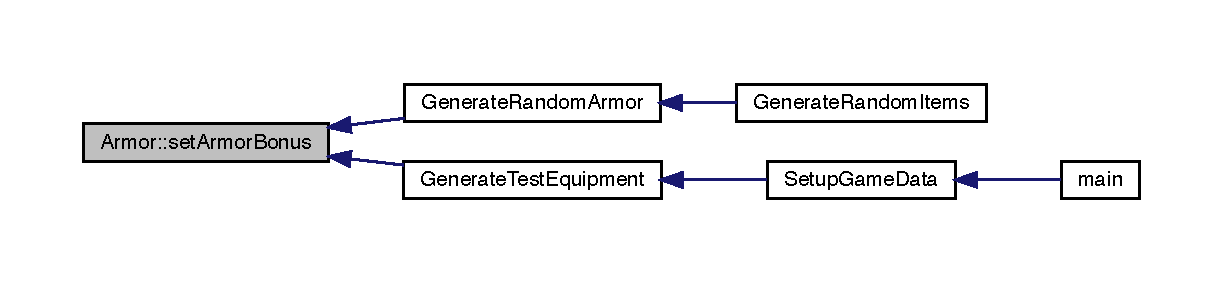
\includegraphics[width=350pt]{d9/d76/class_armor_a14c15f72741f2a3dec28c746b3678c20_icgraph}
\end{center}
\end{figure}
\mbox{\Hypertarget{class_armor_a08f926ae8438bae04058c22b098c6fcf}\label{class_armor_a08f926ae8438bae04058c22b098c6fcf}} 
\index{Armor@{Armor}!set\+Damage\+Reduction@{set\+Damage\+Reduction}}
\index{set\+Damage\+Reduction@{set\+Damage\+Reduction}!Armor@{Armor}}
\subsubsection{\texorpdfstring{set\+Damage\+Reduction()}{setDamageReduction()}}
{\footnotesize\ttfamily void Armor\+::set\+Damage\+Reduction (\begin{DoxyParamCaption}\item[{float}]{value }\end{DoxyParamCaption})}

Here is the caller graph for this function\+:
\nopagebreak
\begin{figure}[H]
\begin{center}
\leavevmode
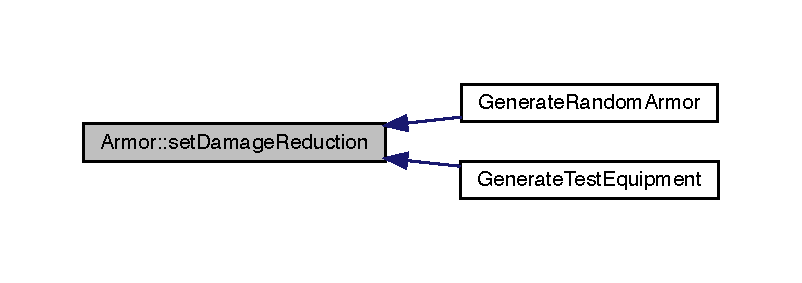
\includegraphics[width=350pt]{d9/d76/class_armor_a08f926ae8438bae04058c22b098c6fcf_icgraph}
\end{center}
\end{figure}
\mbox{\Hypertarget{class_armor_ab48309e3f16d226d56af617c65350698}\label{class_armor_ab48309e3f16d226d56af617c65350698}} 
\index{Armor@{Armor}!set\+Dodge\+Modifier@{set\+Dodge\+Modifier}}
\index{set\+Dodge\+Modifier@{set\+Dodge\+Modifier}!Armor@{Armor}}
\subsubsection{\texorpdfstring{set\+Dodge\+Modifier()}{setDodgeModifier()}}
{\footnotesize\ttfamily void Armor\+::set\+Dodge\+Modifier (\begin{DoxyParamCaption}\item[{float}]{value }\end{DoxyParamCaption})}

Here is the caller graph for this function\+:
\nopagebreak
\begin{figure}[H]
\begin{center}
\leavevmode
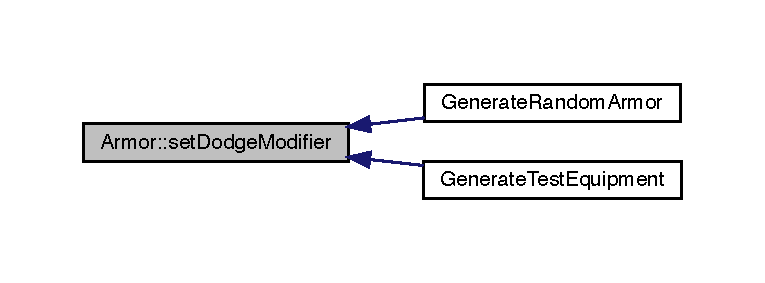
\includegraphics[width=350pt]{d9/d76/class_armor_ab48309e3f16d226d56af617c65350698_icgraph}
\end{center}
\end{figure}
\mbox{\Hypertarget{class_armor_a1710521cbba1bf9328e969cbbc8cdbf3}\label{class_armor_a1710521cbba1bf9328e969cbbc8cdbf3}} 
\index{Armor@{Armor}!set\+Material@{set\+Material}}
\index{set\+Material@{set\+Material}!Armor@{Armor}}
\subsubsection{\texorpdfstring{set\+Material()}{setMaterial()}}
{\footnotesize\ttfamily void Armor\+::set\+Material (\begin{DoxyParamCaption}\item[{\mbox{\hyperlink{class_material}{Material}}}]{value }\end{DoxyParamCaption})}

Here is the call graph for this function\+:
\nopagebreak
\begin{figure}[H]
\begin{center}
\leavevmode
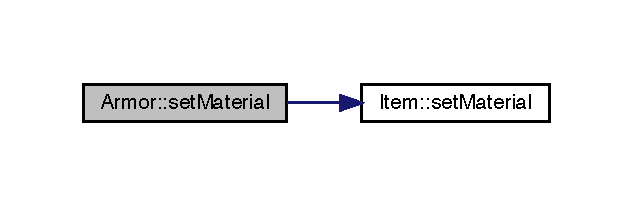
\includegraphics[width=304pt]{d9/d76/class_armor_a1710521cbba1bf9328e969cbbc8cdbf3_cgraph}
\end{center}
\end{figure}
\mbox{\Hypertarget{class_armor_a99475fc688add41f89b7fef160534e33}\label{class_armor_a99475fc688add41f89b7fef160534e33}} 
\index{Armor@{Armor}!set\+Movement\+Modifier@{set\+Movement\+Modifier}}
\index{set\+Movement\+Modifier@{set\+Movement\+Modifier}!Armor@{Armor}}
\subsubsection{\texorpdfstring{set\+Movement\+Modifier()}{setMovementModifier()}}
{\footnotesize\ttfamily void Armor\+::set\+Movement\+Modifier (\begin{DoxyParamCaption}\item[{float}]{value }\end{DoxyParamCaption})}

Here is the caller graph for this function\+:
\nopagebreak
\begin{figure}[H]
\begin{center}
\leavevmode
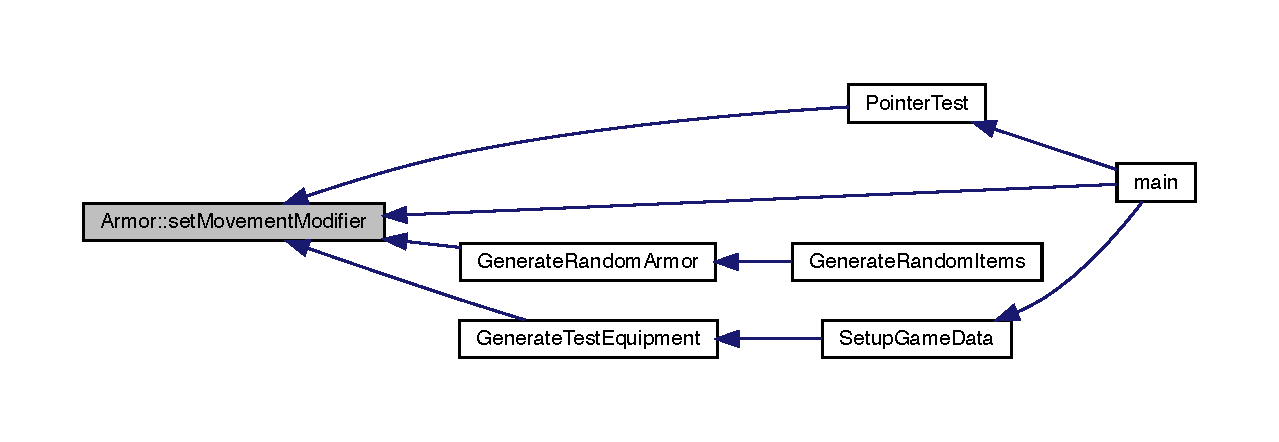
\includegraphics[width=350pt]{d9/d76/class_armor_a99475fc688add41f89b7fef160534e33_icgraph}
\end{center}
\end{figure}
\mbox{\Hypertarget{class_armor_a4fe1507d7aaf280a18e19f51a6f8c42d}\label{class_armor_a4fe1507d7aaf280a18e19f51a6f8c42d}} 
\index{Armor@{Armor}!show\+Item\+Stats@{show\+Item\+Stats}}
\index{show\+Item\+Stats@{show\+Item\+Stats}!Armor@{Armor}}
\subsubsection{\texorpdfstring{show\+Item\+Stats()}{showItemStats()}}
{\footnotesize\ttfamily void Armor\+::show\+Item\+Stats (\begin{DoxyParamCaption}{ }\end{DoxyParamCaption}) const\hspace{0.3cm}{\ttfamily [virtual]}}



Implements \mbox{\hyperlink{class_item_aaf7dae41afdce432c11261043e8e4e30}{Item}}.

Here is the call graph for this function\+:
\nopagebreak
\begin{figure}[H]
\begin{center}
\leavevmode
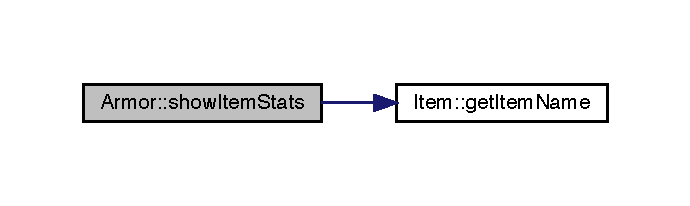
\includegraphics[width=331pt]{d9/d76/class_armor_a4fe1507d7aaf280a18e19f51a6f8c42d_cgraph}
\end{center}
\end{figure}
\mbox{\Hypertarget{class_armor_a72b3d5c0294e80243ed8c96dbc35ccc7}\label{class_armor_a72b3d5c0294e80243ed8c96dbc35ccc7}} 
\index{Armor@{Armor}!si\+Get\+Armor\+Bonus@{si\+Get\+Armor\+Bonus}}
\index{si\+Get\+Armor\+Bonus@{si\+Get\+Armor\+Bonus}!Armor@{Armor}}
\subsubsection{\texorpdfstring{si\+Get\+Armor\+Bonus()}{siGetArmorBonus()}}
{\footnotesize\ttfamily short int Armor\+::si\+Get\+Armor\+Bonus (\begin{DoxyParamCaption}{ }\end{DoxyParamCaption}) const}



\subsection{Friends And Related Function Documentation}
\mbox{\Hypertarget{class_armor_aad85754f188b769ff61150eaf36106c4}\label{class_armor_aad85754f188b769ff61150eaf36106c4}} 
\index{Armor@{Armor}!Item@{Item}}
\index{Item@{Item}!Armor@{Armor}}
\subsubsection{\texorpdfstring{Item}{Item}}
{\footnotesize\ttfamily friend class \mbox{\hyperlink{class_item}{Item}}\hspace{0.3cm}{\ttfamily [friend]}}



\subsection{Member Data Documentation}
\mbox{\Hypertarget{class_armor_acc29c5818b294aaaa11d8d1621b7dd19}\label{class_armor_acc29c5818b294aaaa11d8d1621b7dd19}} 
\index{Armor@{Armor}!f\+Damage\+Reduction@{f\+Damage\+Reduction}}
\index{f\+Damage\+Reduction@{f\+Damage\+Reduction}!Armor@{Armor}}
\subsubsection{\texorpdfstring{f\+Damage\+Reduction}{fDamageReduction}}
{\footnotesize\ttfamily float Armor\+::f\+Damage\+Reduction\hspace{0.3cm}{\ttfamily [private]}}

\mbox{\Hypertarget{class_armor_aed2f98ba9acefdb67ac75104c55ea266}\label{class_armor_aed2f98ba9acefdb67ac75104c55ea266}} 
\index{Armor@{Armor}!f\+Dodge\+Modifier@{f\+Dodge\+Modifier}}
\index{f\+Dodge\+Modifier@{f\+Dodge\+Modifier}!Armor@{Armor}}
\subsubsection{\texorpdfstring{f\+Dodge\+Modifier}{fDodgeModifier}}
{\footnotesize\ttfamily float Armor\+::f\+Dodge\+Modifier\hspace{0.3cm}{\ttfamily [private]}}

\mbox{\Hypertarget{class_armor_aa71e430d9308cfe64b5168014c063722}\label{class_armor_aa71e430d9308cfe64b5168014c063722}} 
\index{Armor@{Armor}!f\+Movement\+Modifier@{f\+Movement\+Modifier}}
\index{f\+Movement\+Modifier@{f\+Movement\+Modifier}!Armor@{Armor}}
\subsubsection{\texorpdfstring{f\+Movement\+Modifier}{fMovementModifier}}
{\footnotesize\ttfamily float Armor\+::f\+Movement\+Modifier\hspace{0.3cm}{\ttfamily [private]}}

\mbox{\Hypertarget{class_armor_a2ebccb72313c650ec1b8bafec4e82dc2}\label{class_armor_a2ebccb72313c650ec1b8bafec4e82dc2}} 
\index{Armor@{Armor}!si\+Armor\+Bonus@{si\+Armor\+Bonus}}
\index{si\+Armor\+Bonus@{si\+Armor\+Bonus}!Armor@{Armor}}
\subsubsection{\texorpdfstring{si\+Armor\+Bonus}{siArmorBonus}}
{\footnotesize\ttfamily short int Armor\+::si\+Armor\+Bonus\hspace{0.3cm}{\ttfamily [private]}}



The documentation for this class was generated from the following files\+:\begin{DoxyCompactItemize}
\item 
/\+Users/\+Afromullet/\+Documents/\+S\+F\+M\+L/\+Colony2/\+Colony/\+Equipment/\mbox{\hyperlink{_armor_8hpp}{Armor.\+hpp}}\item 
/\+Users/\+Afromullet/\+Documents/\+S\+F\+M\+L/\+Colony2/\+Colony/\+Equipment/\mbox{\hyperlink{_armor_8cpp}{Armor.\+cpp}}\end{DoxyCompactItemize}

\hypertarget{struct_a_star_node}{}\section{A\+Star\+Node Struct Reference}
\label{struct_a_star_node}\index{A\+Star\+Node@{A\+Star\+Node}}


{\ttfamily \#include $<$Pathfinding.\+hpp$>$}



Collaboration diagram for A\+Star\+Node\+:
\nopagebreak
\begin{figure}[H]
\begin{center}
\leavevmode
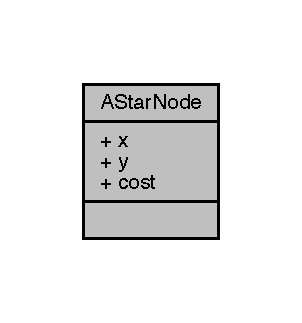
\includegraphics[width=145pt]{df/d44/struct_a_star_node__coll__graph}
\end{center}
\end{figure}
\subsection*{Public Attributes}
\begin{DoxyCompactItemize}
\item 
int \mbox{\hyperlink{struct_a_star_node_a7d4d80244c6ddf6733b70c87dca1a67e}{x}}
\item 
int \mbox{\hyperlink{struct_a_star_node_a9d583c923d4a73876a348299ec54f8c0}{y}}
\item 
int \mbox{\hyperlink{struct_a_star_node_a22e16074f58bbce0b40cb2b141fec3dc}{cost}}
\end{DoxyCompactItemize}


\subsection{Member Data Documentation}
\mbox{\Hypertarget{struct_a_star_node_a22e16074f58bbce0b40cb2b141fec3dc}\label{struct_a_star_node_a22e16074f58bbce0b40cb2b141fec3dc}} 
\index{A\+Star\+Node@{A\+Star\+Node}!cost@{cost}}
\index{cost@{cost}!A\+Star\+Node@{A\+Star\+Node}}
\subsubsection{\texorpdfstring{cost}{cost}}
{\footnotesize\ttfamily int A\+Star\+Node\+::cost}

\mbox{\Hypertarget{struct_a_star_node_a7d4d80244c6ddf6733b70c87dca1a67e}\label{struct_a_star_node_a7d4d80244c6ddf6733b70c87dca1a67e}} 
\index{A\+Star\+Node@{A\+Star\+Node}!x@{x}}
\index{x@{x}!A\+Star\+Node@{A\+Star\+Node}}
\subsubsection{\texorpdfstring{x}{x}}
{\footnotesize\ttfamily int A\+Star\+Node\+::x}

\mbox{\Hypertarget{struct_a_star_node_a9d583c923d4a73876a348299ec54f8c0}\label{struct_a_star_node_a9d583c923d4a73876a348299ec54f8c0}} 
\index{A\+Star\+Node@{A\+Star\+Node}!y@{y}}
\index{y@{y}!A\+Star\+Node@{A\+Star\+Node}}
\subsubsection{\texorpdfstring{y}{y}}
{\footnotesize\ttfamily int A\+Star\+Node\+::y}



The documentation for this struct was generated from the following file\+:\begin{DoxyCompactItemize}
\item 
/\+Users/\+Afromullet/\+Documents/\+S\+F\+M\+L/\+Colony2/\+Colony/\mbox{\hyperlink{_pathfinding_8hpp}{Pathfinding.\+hpp}}\end{DoxyCompactItemize}

\hypertarget{struct_attack_stats}{}\section{Attack\+Stats Struct Reference}
\label{struct_attack_stats}\index{Attack\+Stats@{Attack\+Stats}}


{\ttfamily \#include $<$Enum\+Types.\+hpp$>$}



Collaboration diagram for Attack\+Stats\+:\nopagebreak
\begin{figure}[H]
\begin{center}
\leavevmode
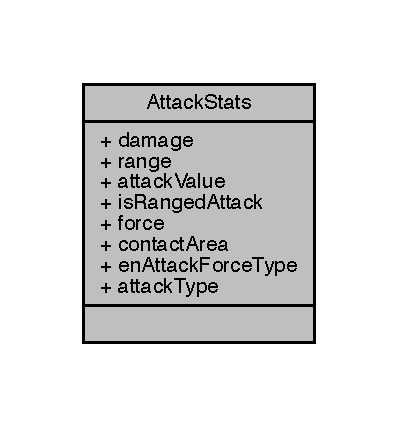
\includegraphics[width=191pt]{d2/d16/struct_attack_stats__coll__graph}
\end{center}
\end{figure}
\subsection*{Public Attributes}
\begin{DoxyCompactItemize}
\item 
int \mbox{\hyperlink{struct_attack_stats_a358d827a9c95797171c79cecb4f907de}{damage}}
\item 
int \mbox{\hyperlink{struct_attack_stats_a6c771cd1408f202aa1c6b8bb0fff353b}{range}}
\item 
int \mbox{\hyperlink{struct_attack_stats_ae16d335630c1ff94a4147c9484818d35}{attack\+Value}}
\item 
bool \mbox{\hyperlink{struct_attack_stats_ae520cb405184191eef7d816e6ade41e4}{is\+Ranged\+Attack}}
\item 
float \mbox{\hyperlink{struct_attack_stats_ab351196c612dedf32664a1f1c98f49d0}{force}}
\item 
float \mbox{\hyperlink{struct_attack_stats_afaa92e7e1949f50eb1f6f4c6552265ba}{contact\+Area}}
\item 
\mbox{\hyperlink{_enum_types_8hpp_ad893f9959c49f07fb713f13630b7ee2d}{Attack\+Force\+Type}} \mbox{\hyperlink{struct_attack_stats_a9b9650abd264559a4a8914a67b070c1e}{en\+Attack\+Force\+Type}}
\item 
\mbox{\hyperlink{_enum_types_8hpp_a904b2f9c8f3951116c343784c59d6afe}{Attack\+Type}} \mbox{\hyperlink{struct_attack_stats_aacd65c62b2bc2d112d83a281940c6427}{attack\+Type}}
\end{DoxyCompactItemize}


\subsection{Member Data Documentation}
\mbox{\Hypertarget{struct_attack_stats_aacd65c62b2bc2d112d83a281940c6427}\label{struct_attack_stats_aacd65c62b2bc2d112d83a281940c6427}} 
\index{Attack\+Stats@{Attack\+Stats}!attack\+Type@{attack\+Type}}
\index{attack\+Type@{attack\+Type}!Attack\+Stats@{Attack\+Stats}}
\subsubsection{\texorpdfstring{attack\+Type}{attackType}}
{\footnotesize\ttfamily \mbox{\hyperlink{_enum_types_8hpp_a904b2f9c8f3951116c343784c59d6afe}{Attack\+Type}} Attack\+Stats\+::attack\+Type}

\mbox{\Hypertarget{struct_attack_stats_ae16d335630c1ff94a4147c9484818d35}\label{struct_attack_stats_ae16d335630c1ff94a4147c9484818d35}} 
\index{Attack\+Stats@{Attack\+Stats}!attack\+Value@{attack\+Value}}
\index{attack\+Value@{attack\+Value}!Attack\+Stats@{Attack\+Stats}}
\subsubsection{\texorpdfstring{attack\+Value}{attackValue}}
{\footnotesize\ttfamily int Attack\+Stats\+::attack\+Value}

\mbox{\Hypertarget{struct_attack_stats_afaa92e7e1949f50eb1f6f4c6552265ba}\label{struct_attack_stats_afaa92e7e1949f50eb1f6f4c6552265ba}} 
\index{Attack\+Stats@{Attack\+Stats}!contact\+Area@{contact\+Area}}
\index{contact\+Area@{contact\+Area}!Attack\+Stats@{Attack\+Stats}}
\subsubsection{\texorpdfstring{contact\+Area}{contactArea}}
{\footnotesize\ttfamily float Attack\+Stats\+::contact\+Area}

\mbox{\Hypertarget{struct_attack_stats_a358d827a9c95797171c79cecb4f907de}\label{struct_attack_stats_a358d827a9c95797171c79cecb4f907de}} 
\index{Attack\+Stats@{Attack\+Stats}!damage@{damage}}
\index{damage@{damage}!Attack\+Stats@{Attack\+Stats}}
\subsubsection{\texorpdfstring{damage}{damage}}
{\footnotesize\ttfamily int Attack\+Stats\+::damage}

\mbox{\Hypertarget{struct_attack_stats_a9b9650abd264559a4a8914a67b070c1e}\label{struct_attack_stats_a9b9650abd264559a4a8914a67b070c1e}} 
\index{Attack\+Stats@{Attack\+Stats}!en\+Attack\+Force\+Type@{en\+Attack\+Force\+Type}}
\index{en\+Attack\+Force\+Type@{en\+Attack\+Force\+Type}!Attack\+Stats@{Attack\+Stats}}
\subsubsection{\texorpdfstring{en\+Attack\+Force\+Type}{enAttackForceType}}
{\footnotesize\ttfamily \mbox{\hyperlink{_enum_types_8hpp_ad893f9959c49f07fb713f13630b7ee2d}{Attack\+Force\+Type}} Attack\+Stats\+::en\+Attack\+Force\+Type}

\mbox{\Hypertarget{struct_attack_stats_ab351196c612dedf32664a1f1c98f49d0}\label{struct_attack_stats_ab351196c612dedf32664a1f1c98f49d0}} 
\index{Attack\+Stats@{Attack\+Stats}!force@{force}}
\index{force@{force}!Attack\+Stats@{Attack\+Stats}}
\subsubsection{\texorpdfstring{force}{force}}
{\footnotesize\ttfamily float Attack\+Stats\+::force}

\mbox{\Hypertarget{struct_attack_stats_ae520cb405184191eef7d816e6ade41e4}\label{struct_attack_stats_ae520cb405184191eef7d816e6ade41e4}} 
\index{Attack\+Stats@{Attack\+Stats}!is\+Ranged\+Attack@{is\+Ranged\+Attack}}
\index{is\+Ranged\+Attack@{is\+Ranged\+Attack}!Attack\+Stats@{Attack\+Stats}}
\subsubsection{\texorpdfstring{is\+Ranged\+Attack}{isRangedAttack}}
{\footnotesize\ttfamily bool Attack\+Stats\+::is\+Ranged\+Attack}

\mbox{\Hypertarget{struct_attack_stats_a6c771cd1408f202aa1c6b8bb0fff353b}\label{struct_attack_stats_a6c771cd1408f202aa1c6b8bb0fff353b}} 
\index{Attack\+Stats@{Attack\+Stats}!range@{range}}
\index{range@{range}!Attack\+Stats@{Attack\+Stats}}
\subsubsection{\texorpdfstring{range}{range}}
{\footnotesize\ttfamily int Attack\+Stats\+::range}



The documentation for this struct was generated from the following file\+:\begin{DoxyCompactItemize}
\item 
/\+Users/\+Afromullet/\+Documents/\+S\+F\+M\+L/\+Colony2/\+Colony/\+Defs/\mbox{\hyperlink{_enum_types_8hpp}{Enum\+Types.\+hpp}}\end{DoxyCompactItemize}

\hypertarget{class_base_creature}{}\section{Base\+Creature Class Reference}
\label{class_base_creature}\index{Base\+Creature@{Base\+Creature}}


{\ttfamily \#include $<$Base\+Creature.\+hpp$>$}



Collaboration diagram for Base\+Creature\+:
\nopagebreak
\begin{figure}[H]
\begin{center}
\leavevmode
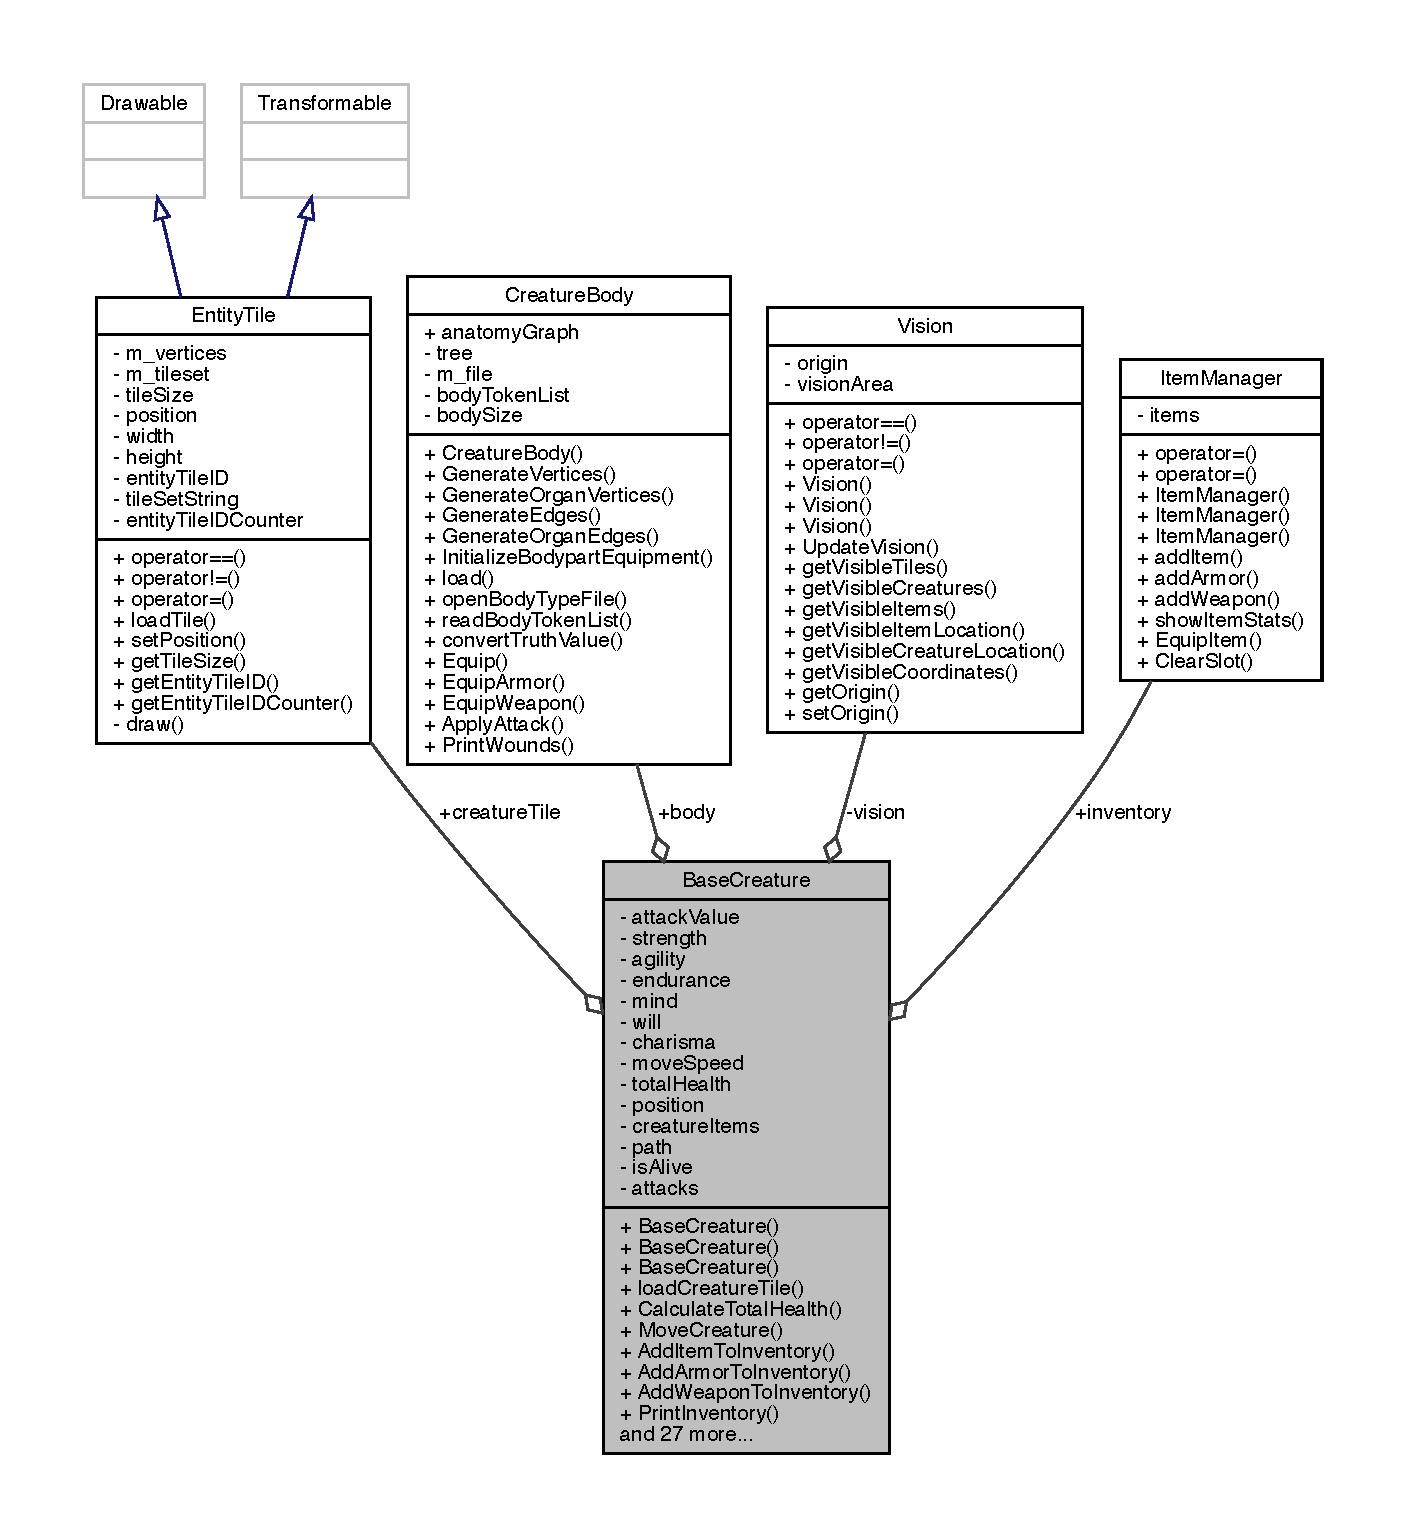
\includegraphics[width=350pt]{d9/d23/class_base_creature__coll__graph}
\end{center}
\end{figure}
\subsection*{Public Member Functions}
\begin{DoxyCompactItemize}
\item 
\mbox{\hyperlink{class_base_creature_aed503a9552a9d28233012f7a7b74d9bc}{Base\+Creature}} ()
\item 
\mbox{\hyperlink{class_base_creature_adda13b6dcb4365d47210e34f2dcdc8ba}{Base\+Creature}} (const \mbox{\hyperlink{class_base_creature}{Base\+Creature}} \&other)
\item 
\mbox{\hyperlink{class_base_creature_aa496d94797fc52d3db909b78d8ee24d4}{Base\+Creature}} (\mbox{\hyperlink{class_base_creature}{Base\+Creature}} \&other)
\item 
void \mbox{\hyperlink{class_base_creature_af2066b8eb62bf595d30feae6671e4495}{load\+Creature\+Tile}} (const std\+::string \&tileset, int tile\+X\+Size, int tile\+Y\+Size)
\item 
void \mbox{\hyperlink{class_base_creature_ac5c9f52046801eb47701ef8b0f1eb32c}{Calculate\+Total\+Health}} ()
\item 
bool \mbox{\hyperlink{class_base_creature_a77f0a7d7c441406c252c3278817454d8}{Move\+Creature}} (int x, int y)
\item 
void \mbox{\hyperlink{class_base_creature_ab6f0139afb4e1b15d5f1feecc267580d}{Add\+Item\+To\+Inventory}} (\mbox{\hyperlink{class_item}{Item}} $\ast$item)
\item 
void \mbox{\hyperlink{class_base_creature_a03122a2c070fe7cab0dc772f552f1a63}{Add\+Armor\+To\+Inventory}} (\mbox{\hyperlink{class_armor}{Armor}} val)
\item 
void \mbox{\hyperlink{class_base_creature_ab0a90200835bc80c6db29e31f98d35e9}{Add\+Weapon\+To\+Inventory}} (\mbox{\hyperlink{class_weapon}{Weapon}} val)
\item 
void \mbox{\hyperlink{class_base_creature_a097ec44d0b215f75ca75ae69c2bd11be}{Print\+Inventory}} ()
\item 
void \mbox{\hyperlink{class_base_creature_ac3d7907a8d8e0967a5881ff180205028}{Print\+Equipment}} ()
\item 
void \mbox{\hyperlink{class_base_creature_a82807038eafe46f7ac510a99a4cdc25e}{Equip}} (\mbox{\hyperlink{class_item}{Item}} $\ast$item)
\item 
void \mbox{\hyperlink{class_base_creature_a637cb7174d9bb9677a21281ff19fb10a}{Equip\+Item\+From\+Inventory}} (int n)
\item 
void \mbox{\hyperlink{class_base_creature_a1e73375251b20070ae9dac505b280b3e}{Equip\+Item}} (int i)
\item 
void \mbox{\hyperlink{class_base_creature_a2d45724079ff2eeb6606b222e405e4a8}{Pickup\+Item}} (\mbox{\hyperlink{class_map}{Map}} \&map, std\+::list$<$ \mbox{\hyperlink{class_item}{Item}} $\ast$$>$ \&item\+List)
\item 
void \mbox{\hyperlink{class_base_creature_a63f43a7153eee3c1032b02f6d1948cdb}{Attack\+Creature}} (int attack\+Bonus, int damage)
\item 
void \mbox{\hyperlink{class_base_creature_aa18f395754df39095f993e6805ef37a8}{Add\+To\+Path}} (sf\+::\+Vector2i point)
\item 
void \mbox{\hyperlink{class_base_creature_aaecab78bf5a5a5293079634e813f854f}{Walk\+Path}} (\mbox{\hyperlink{class_map}{Map}} \&map)
\item 
void \mbox{\hyperlink{class_base_creature_a8c7fec43bb0ca9a15e0f2596960283b7}{clear\+Path}} ()
\item 
void \mbox{\hyperlink{class_base_creature_a389d8ae4c4caa2d7c55939bef70935a8}{calculate\+Attack\+Parameters}} ()
\item 
float \mbox{\hyperlink{class_base_creature_ac81e681e444ed860c212463025d04a1d}{Calculate\+Melee\+Attack\+Force}} (\mbox{\hyperlink{class_weapon}{Weapon}} \&weapon)
\item 
short int \mbox{\hyperlink{class_base_creature_a7b4f974b77953aea8f4c698e6e21c500}{get\+Melee\+Attack\+Value}} () const
\item 
short int \mbox{\hyperlink{class_base_creature_a58a174420d25df7d0865087586c66a21}{get\+Ranged\+Attack\+Value}} () const
\item 
short int \mbox{\hyperlink{class_base_creature_a1232a2ecb3199fe79627df912078f24e}{get\+Strength}} () const
\item 
short int \mbox{\hyperlink{class_base_creature_ac04efe1dda147e264998609635baadb6}{get\+Agility}} () const
\item 
short int \mbox{\hyperlink{class_base_creature_a4e3864bd12e271718a838ba6c3881f0a}{get\+Attack\+Value}} () const
\item 
sf\+::\+Vector2i \mbox{\hyperlink{class_base_creature_a00ebdc186dd6d3c0ef3c3d1262d4363f}{get\+Position}} () const
\item 
std\+::string \mbox{\hyperlink{class_base_creature_a19f380cccb11f31d10d00de934da1b7f}{Get\+Item\+Info}} (int n)
\item 
int \mbox{\hyperlink{class_base_creature_accab7a878eae0580476b282ce2c556d3}{get\+Total\+Health}} () const
\item 
std\+::list$<$ \mbox{\hyperlink{class_item}{Item}} $\ast$ $>$ \mbox{\hyperlink{class_base_creature_a505e70415a3e2db87aac0767498375ff}{get\+Inventory}} ()
\item 
\mbox{\hyperlink{class_vision}{Vision}} \& \mbox{\hyperlink{class_base_creature_a8a960bc7a7689f5633b1abaa82fa6e95}{get\+Vision}} ()
\item 
std\+::vector$<$ \mbox{\hyperlink{struct_attack_stats}{Attack\+Stats}} $>$ \& \mbox{\hyperlink{class_base_creature_ae2fdab903403a68e431baa080f715d3c}{get\+Attacks}} ()
\item 
void \mbox{\hyperlink{class_base_creature_a00ffc1ee732a8f0a8921c9cee6842e4d}{set\+Position}} (short int x, short int y)
\item 
void \mbox{\hyperlink{class_base_creature_ae1cb6e6d01d0c369433fb1fb20803f91}{set\+Velocity}} (int x, int y)
\item 
void \mbox{\hyperlink{class_base_creature_a3a2eb318b9c5d849a02884b20e32f83d}{set\+Strength}} (int \+\_\+strength)
\item 
void \mbox{\hyperlink{class_base_creature_ad6357a6d4456d0b669abd1675efcca30}{set\+Agility}} (int \+\_\+agility)
\item 
void \mbox{\hyperlink{class_base_creature_a82f847585033035597700b071e40611f}{set\+Total\+Health}} (int \+\_\+health)
\end{DoxyCompactItemize}
\subsection*{Public Attributes}
\begin{DoxyCompactItemize}
\item 
\mbox{\hyperlink{class_item_manager}{Item\+Manager}} \mbox{\hyperlink{class_base_creature_aa5945485ad5e5974f2600fec2f0a8627}{inventory}}
\item 
\mbox{\hyperlink{class_creature_body}{Creature\+Body}} \mbox{\hyperlink{class_base_creature_a97e1d629325177b201bdcd43addefd0d}{body}}
\item 
\mbox{\hyperlink{class_entity_tile}{Entity\+Tile}} \mbox{\hyperlink{class_base_creature_a35d7353131ee00fe8738ec5a5ebfe231}{creature\+Tile}}
\end{DoxyCompactItemize}
\subsection*{Private Attributes}
\begin{DoxyCompactItemize}
\item 
short int \mbox{\hyperlink{class_base_creature_ac5a9c850146fa856dbf7fdd0def635ac}{attack\+Value}}
\item 
short int \mbox{\hyperlink{class_base_creature_a7f325c07376932d6e831dd00a350b806}{strength}}
\item 
short int \mbox{\hyperlink{class_base_creature_a23bbce83de8f7be2dfbcec7f5da223ab}{agility}}
\item 
short int \mbox{\hyperlink{class_base_creature_a74bc0648b11f9637b31ad5b76f056740}{endurance}}
\item 
short int \mbox{\hyperlink{class_base_creature_a8debd17b675db2ac6d944e2ccb314def}{mind}}
\item 
short int \mbox{\hyperlink{class_base_creature_a992cbd3a6be93279f2c933a50eba5000}{will}}
\item 
short int \mbox{\hyperlink{class_base_creature_aa62b65a4bd43be6e999d9a29a472fffe}{charisma}}
\item 
short int \mbox{\hyperlink{class_base_creature_a846cd45ba49c6496bdcb760651b9aaa8}{move\+Speed}}
\item 
int \mbox{\hyperlink{class_base_creature_a727462587a0ec421c549acf8c497de42}{total\+Health}}
\item 
sf\+::\+Vector2i \mbox{\hyperlink{class_base_creature_ac0aa7211db6bbc4033b0a11e6c34171b}{position}}
\item 
std\+::list$<$ \mbox{\hyperlink{class_item}{Item}} $\ast$ $>$ \mbox{\hyperlink{class_base_creature_a15a7a38b2a5bc15d1c3f8eda7e1d835b}{creature\+Items}}
\item 
std\+::queue$<$ sf\+::\+Vector2i $>$ \mbox{\hyperlink{class_base_creature_a0e419167e4986de0a4652b8979d66e16}{path}}
\item 
\mbox{\hyperlink{class_vision}{Vision}} \mbox{\hyperlink{class_base_creature_a8433c26fcbcb9bee87c35b15ae2e0814}{vision}}
\item 
bool \mbox{\hyperlink{class_base_creature_adeb6eed7546d84b1547e8134f582a6c7}{is\+Alive}}
\item 
std\+::vector$<$ \mbox{\hyperlink{struct_attack_stats}{Attack\+Stats}} $>$ \mbox{\hyperlink{class_base_creature_ab40c21845e4c19538b356bbcb01f7075}{attacks}}
\end{DoxyCompactItemize}


\subsection{Constructor \& Destructor Documentation}
\mbox{\Hypertarget{class_base_creature_aed503a9552a9d28233012f7a7b74d9bc}\label{class_base_creature_aed503a9552a9d28233012f7a7b74d9bc}} 
\index{Base\+Creature@{Base\+Creature}!Base\+Creature@{Base\+Creature}}
\index{Base\+Creature@{Base\+Creature}!Base\+Creature@{Base\+Creature}}
\subsubsection{\texorpdfstring{Base\+Creature()}{BaseCreature()}\hspace{0.1cm}{\footnotesize\ttfamily [1/3]}}
{\footnotesize\ttfamily Base\+Creature\+::\+Base\+Creature (\begin{DoxyParamCaption}{ }\end{DoxyParamCaption})}

\mbox{\Hypertarget{class_base_creature_adda13b6dcb4365d47210e34f2dcdc8ba}\label{class_base_creature_adda13b6dcb4365d47210e34f2dcdc8ba}} 
\index{Base\+Creature@{Base\+Creature}!Base\+Creature@{Base\+Creature}}
\index{Base\+Creature@{Base\+Creature}!Base\+Creature@{Base\+Creature}}
\subsubsection{\texorpdfstring{Base\+Creature()}{BaseCreature()}\hspace{0.1cm}{\footnotesize\ttfamily [2/3]}}
{\footnotesize\ttfamily Base\+Creature\+::\+Base\+Creature (\begin{DoxyParamCaption}\item[{const \mbox{\hyperlink{class_base_creature}{Base\+Creature}} \&}]{other }\end{DoxyParamCaption})}

\mbox{\Hypertarget{class_base_creature_aa496d94797fc52d3db909b78d8ee24d4}\label{class_base_creature_aa496d94797fc52d3db909b78d8ee24d4}} 
\index{Base\+Creature@{Base\+Creature}!Base\+Creature@{Base\+Creature}}
\index{Base\+Creature@{Base\+Creature}!Base\+Creature@{Base\+Creature}}
\subsubsection{\texorpdfstring{Base\+Creature()}{BaseCreature()}\hspace{0.1cm}{\footnotesize\ttfamily [3/3]}}
{\footnotesize\ttfamily Base\+Creature\+::\+Base\+Creature (\begin{DoxyParamCaption}\item[{\mbox{\hyperlink{class_base_creature}{Base\+Creature}} \&}]{other }\end{DoxyParamCaption})}



\subsection{Member Function Documentation}
\mbox{\Hypertarget{class_base_creature_a03122a2c070fe7cab0dc772f552f1a63}\label{class_base_creature_a03122a2c070fe7cab0dc772f552f1a63}} 
\index{Base\+Creature@{Base\+Creature}!Add\+Armor\+To\+Inventory@{Add\+Armor\+To\+Inventory}}
\index{Add\+Armor\+To\+Inventory@{Add\+Armor\+To\+Inventory}!Base\+Creature@{Base\+Creature}}
\subsubsection{\texorpdfstring{Add\+Armor\+To\+Inventory()}{AddArmorToInventory()}}
{\footnotesize\ttfamily void Base\+Creature\+::\+Add\+Armor\+To\+Inventory (\begin{DoxyParamCaption}\item[{\mbox{\hyperlink{class_armor}{Armor}}}]{val }\end{DoxyParamCaption})}

Here is the call graph for this function\+:
\nopagebreak
\begin{figure}[H]
\begin{center}
\leavevmode
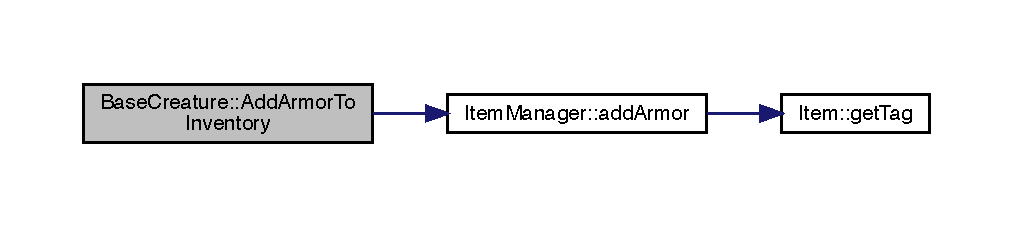
\includegraphics[width=350pt]{d2/d3b/class_base_creature_a03122a2c070fe7cab0dc772f552f1a63_cgraph}
\end{center}
\end{figure}
Here is the caller graph for this function\+:
\nopagebreak
\begin{figure}[H]
\begin{center}
\leavevmode
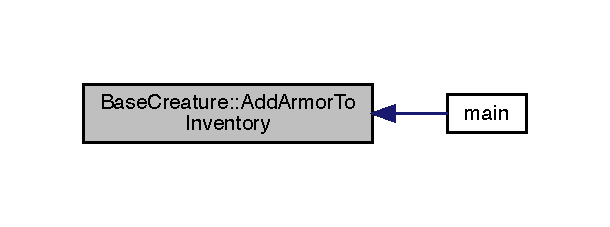
\includegraphics[width=293pt]{d2/d3b/class_base_creature_a03122a2c070fe7cab0dc772f552f1a63_icgraph}
\end{center}
\end{figure}
\mbox{\Hypertarget{class_base_creature_ab6f0139afb4e1b15d5f1feecc267580d}\label{class_base_creature_ab6f0139afb4e1b15d5f1feecc267580d}} 
\index{Base\+Creature@{Base\+Creature}!Add\+Item\+To\+Inventory@{Add\+Item\+To\+Inventory}}
\index{Add\+Item\+To\+Inventory@{Add\+Item\+To\+Inventory}!Base\+Creature@{Base\+Creature}}
\subsubsection{\texorpdfstring{Add\+Item\+To\+Inventory()}{AddItemToInventory()}}
{\footnotesize\ttfamily void Base\+Creature\+::\+Add\+Item\+To\+Inventory (\begin{DoxyParamCaption}\item[{\mbox{\hyperlink{class_item}{Item}} $\ast$}]{item }\end{DoxyParamCaption})}

Here is the caller graph for this function\+:
\nopagebreak
\begin{figure}[H]
\begin{center}
\leavevmode
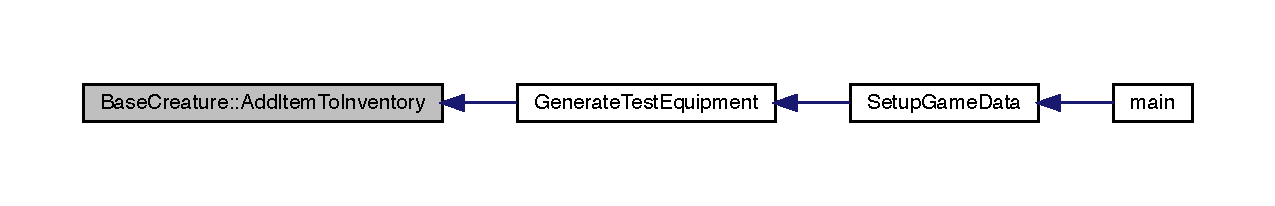
\includegraphics[width=350pt]{d2/d3b/class_base_creature_ab6f0139afb4e1b15d5f1feecc267580d_icgraph}
\end{center}
\end{figure}
\mbox{\Hypertarget{class_base_creature_aa18f395754df39095f993e6805ef37a8}\label{class_base_creature_aa18f395754df39095f993e6805ef37a8}} 
\index{Base\+Creature@{Base\+Creature}!Add\+To\+Path@{Add\+To\+Path}}
\index{Add\+To\+Path@{Add\+To\+Path}!Base\+Creature@{Base\+Creature}}
\subsubsection{\texorpdfstring{Add\+To\+Path()}{AddToPath()}}
{\footnotesize\ttfamily void Base\+Creature\+::\+Add\+To\+Path (\begin{DoxyParamCaption}\item[{sf\+::\+Vector2i}]{point }\end{DoxyParamCaption})}

Here is the caller graph for this function\+:
\nopagebreak
\begin{figure}[H]
\begin{center}
\leavevmode
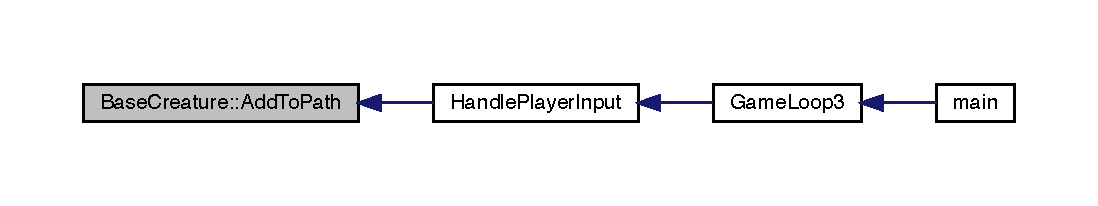
\includegraphics[width=350pt]{d2/d3b/class_base_creature_aa18f395754df39095f993e6805ef37a8_icgraph}
\end{center}
\end{figure}
\mbox{\Hypertarget{class_base_creature_ab0a90200835bc80c6db29e31f98d35e9}\label{class_base_creature_ab0a90200835bc80c6db29e31f98d35e9}} 
\index{Base\+Creature@{Base\+Creature}!Add\+Weapon\+To\+Inventory@{Add\+Weapon\+To\+Inventory}}
\index{Add\+Weapon\+To\+Inventory@{Add\+Weapon\+To\+Inventory}!Base\+Creature@{Base\+Creature}}
\subsubsection{\texorpdfstring{Add\+Weapon\+To\+Inventory()}{AddWeaponToInventory()}}
{\footnotesize\ttfamily void Base\+Creature\+::\+Add\+Weapon\+To\+Inventory (\begin{DoxyParamCaption}\item[{\mbox{\hyperlink{class_weapon}{Weapon}}}]{val }\end{DoxyParamCaption})}

Here is the call graph for this function\+:
\nopagebreak
\begin{figure}[H]
\begin{center}
\leavevmode
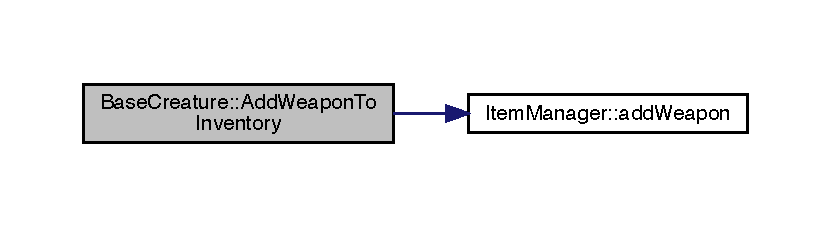
\includegraphics[width=350pt]{d2/d3b/class_base_creature_ab0a90200835bc80c6db29e31f98d35e9_cgraph}
\end{center}
\end{figure}
Here is the caller graph for this function\+:
\nopagebreak
\begin{figure}[H]
\begin{center}
\leavevmode
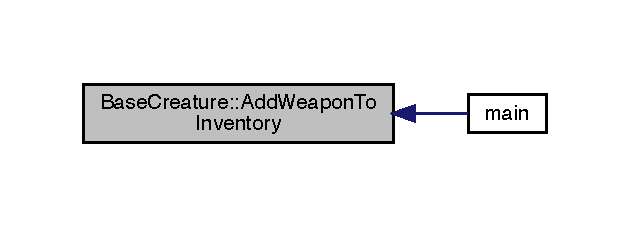
\includegraphics[width=302pt]{d2/d3b/class_base_creature_ab0a90200835bc80c6db29e31f98d35e9_icgraph}
\end{center}
\end{figure}
\mbox{\Hypertarget{class_base_creature_a63f43a7153eee3c1032b02f6d1948cdb}\label{class_base_creature_a63f43a7153eee3c1032b02f6d1948cdb}} 
\index{Base\+Creature@{Base\+Creature}!Attack\+Creature@{Attack\+Creature}}
\index{Attack\+Creature@{Attack\+Creature}!Base\+Creature@{Base\+Creature}}
\subsubsection{\texorpdfstring{Attack\+Creature()}{AttackCreature()}}
{\footnotesize\ttfamily void Base\+Creature\+::\+Attack\+Creature (\begin{DoxyParamCaption}\item[{int}]{attack\+Bonus,  }\item[{int}]{damage }\end{DoxyParamCaption})}

\mbox{\Hypertarget{class_base_creature_a389d8ae4c4caa2d7c55939bef70935a8}\label{class_base_creature_a389d8ae4c4caa2d7c55939bef70935a8}} 
\index{Base\+Creature@{Base\+Creature}!calculate\+Attack\+Parameters@{calculate\+Attack\+Parameters}}
\index{calculate\+Attack\+Parameters@{calculate\+Attack\+Parameters}!Base\+Creature@{Base\+Creature}}
\subsubsection{\texorpdfstring{calculate\+Attack\+Parameters()}{calculateAttackParameters()}}
{\footnotesize\ttfamily void Base\+Creature\+::calculate\+Attack\+Parameters (\begin{DoxyParamCaption}{ }\end{DoxyParamCaption})}

Here is the call graph for this function\+:
\nopagebreak
\begin{figure}[H]
\begin{center}
\leavevmode
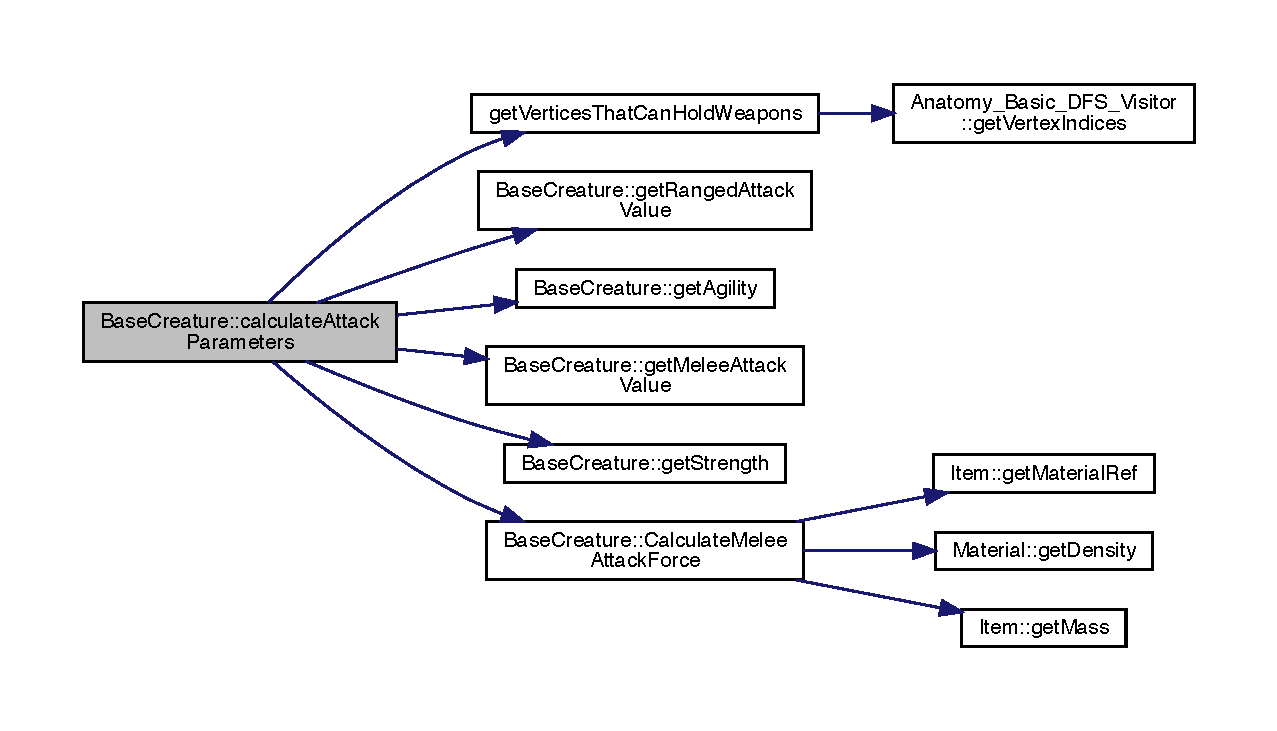
\includegraphics[width=350pt]{d2/d3b/class_base_creature_a389d8ae4c4caa2d7c55939bef70935a8_cgraph}
\end{center}
\end{figure}
Here is the caller graph for this function\+:
\nopagebreak
\begin{figure}[H]
\begin{center}
\leavevmode
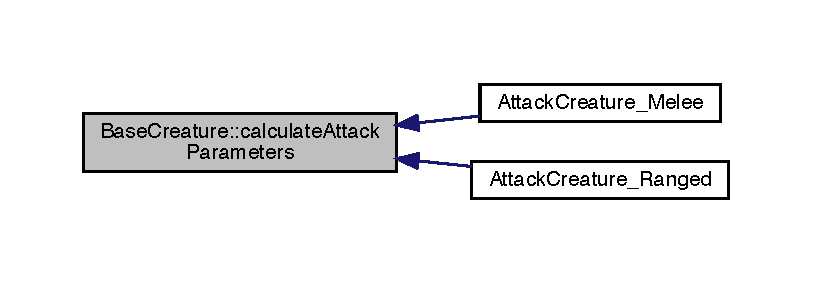
\includegraphics[width=350pt]{d2/d3b/class_base_creature_a389d8ae4c4caa2d7c55939bef70935a8_icgraph}
\end{center}
\end{figure}
\mbox{\Hypertarget{class_base_creature_ac81e681e444ed860c212463025d04a1d}\label{class_base_creature_ac81e681e444ed860c212463025d04a1d}} 
\index{Base\+Creature@{Base\+Creature}!Calculate\+Melee\+Attack\+Force@{Calculate\+Melee\+Attack\+Force}}
\index{Calculate\+Melee\+Attack\+Force@{Calculate\+Melee\+Attack\+Force}!Base\+Creature@{Base\+Creature}}
\subsubsection{\texorpdfstring{Calculate\+Melee\+Attack\+Force()}{CalculateMeleeAttackForce()}}
{\footnotesize\ttfamily float Base\+Creature\+::\+Calculate\+Melee\+Attack\+Force (\begin{DoxyParamCaption}\item[{\mbox{\hyperlink{class_weapon}{Weapon}} \&}]{weapon }\end{DoxyParamCaption})}

Here is the call graph for this function\+:
\nopagebreak
\begin{figure}[H]
\begin{center}
\leavevmode
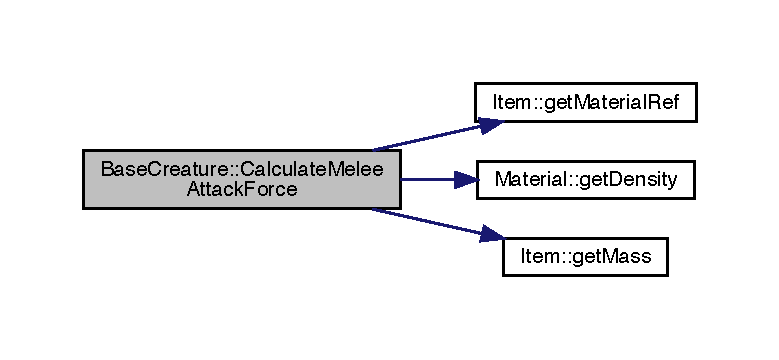
\includegraphics[width=350pt]{d2/d3b/class_base_creature_ac81e681e444ed860c212463025d04a1d_cgraph}
\end{center}
\end{figure}
Here is the caller graph for this function\+:
\nopagebreak
\begin{figure}[H]
\begin{center}
\leavevmode
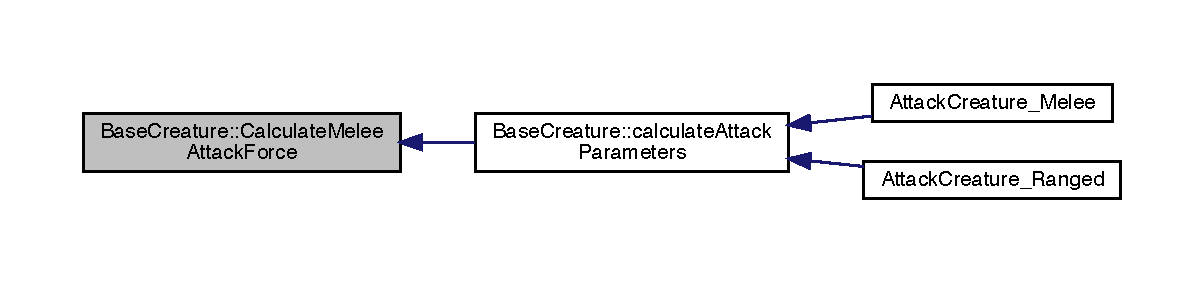
\includegraphics[width=350pt]{d2/d3b/class_base_creature_ac81e681e444ed860c212463025d04a1d_icgraph}
\end{center}
\end{figure}
\mbox{\Hypertarget{class_base_creature_ac5c9f52046801eb47701ef8b0f1eb32c}\label{class_base_creature_ac5c9f52046801eb47701ef8b0f1eb32c}} 
\index{Base\+Creature@{Base\+Creature}!Calculate\+Total\+Health@{Calculate\+Total\+Health}}
\index{Calculate\+Total\+Health@{Calculate\+Total\+Health}!Base\+Creature@{Base\+Creature}}
\subsubsection{\texorpdfstring{Calculate\+Total\+Health()}{CalculateTotalHealth()}}
{\footnotesize\ttfamily void Base\+Creature\+::\+Calculate\+Total\+Health (\begin{DoxyParamCaption}{ }\end{DoxyParamCaption})}

\mbox{\Hypertarget{class_base_creature_a8c7fec43bb0ca9a15e0f2596960283b7}\label{class_base_creature_a8c7fec43bb0ca9a15e0f2596960283b7}} 
\index{Base\+Creature@{Base\+Creature}!clear\+Path@{clear\+Path}}
\index{clear\+Path@{clear\+Path}!Base\+Creature@{Base\+Creature}}
\subsubsection{\texorpdfstring{clear\+Path()}{clearPath()}}
{\footnotesize\ttfamily void Base\+Creature\+::clear\+Path (\begin{DoxyParamCaption}{ }\end{DoxyParamCaption})}

\mbox{\Hypertarget{class_base_creature_a82807038eafe46f7ac510a99a4cdc25e}\label{class_base_creature_a82807038eafe46f7ac510a99a4cdc25e}} 
\index{Base\+Creature@{Base\+Creature}!Equip@{Equip}}
\index{Equip@{Equip}!Base\+Creature@{Base\+Creature}}
\subsubsection{\texorpdfstring{Equip()}{Equip()}}
{\footnotesize\ttfamily void Base\+Creature\+::\+Equip (\begin{DoxyParamCaption}\item[{\mbox{\hyperlink{class_item}{Item}} $\ast$}]{item }\end{DoxyParamCaption})}

\mbox{\Hypertarget{class_base_creature_a1e73375251b20070ae9dac505b280b3e}\label{class_base_creature_a1e73375251b20070ae9dac505b280b3e}} 
\index{Base\+Creature@{Base\+Creature}!Equip\+Item@{Equip\+Item}}
\index{Equip\+Item@{Equip\+Item}!Base\+Creature@{Base\+Creature}}
\subsubsection{\texorpdfstring{Equip\+Item()}{EquipItem()}}
{\footnotesize\ttfamily void Base\+Creature\+::\+Equip\+Item (\begin{DoxyParamCaption}\item[{int}]{i }\end{DoxyParamCaption})}

Here is the call graph for this function\+:
\nopagebreak
\begin{figure}[H]
\begin{center}
\leavevmode
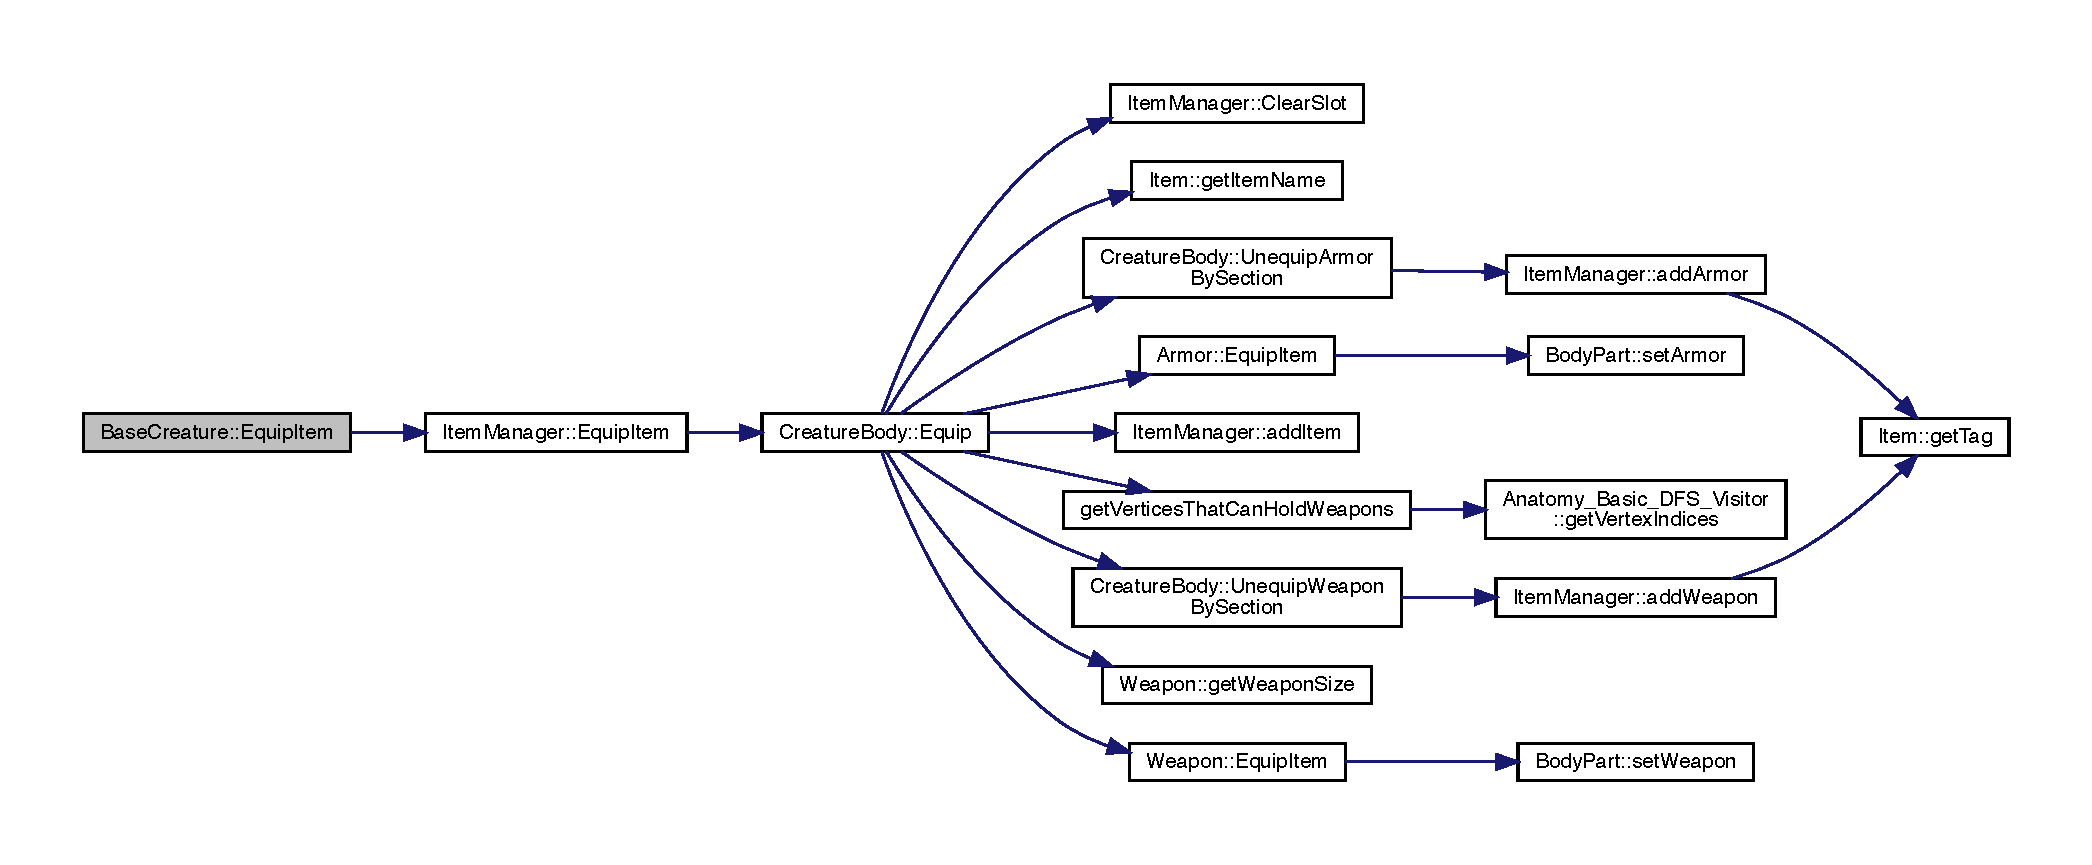
\includegraphics[width=350pt]{d2/d3b/class_base_creature_a1e73375251b20070ae9dac505b280b3e_cgraph}
\end{center}
\end{figure}
Here is the caller graph for this function\+:
\nopagebreak
\begin{figure}[H]
\begin{center}
\leavevmode
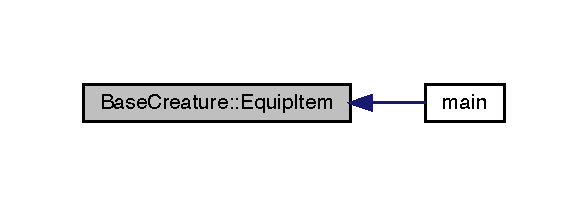
\includegraphics[width=282pt]{d2/d3b/class_base_creature_a1e73375251b20070ae9dac505b280b3e_icgraph}
\end{center}
\end{figure}
\mbox{\Hypertarget{class_base_creature_a637cb7174d9bb9677a21281ff19fb10a}\label{class_base_creature_a637cb7174d9bb9677a21281ff19fb10a}} 
\index{Base\+Creature@{Base\+Creature}!Equip\+Item\+From\+Inventory@{Equip\+Item\+From\+Inventory}}
\index{Equip\+Item\+From\+Inventory@{Equip\+Item\+From\+Inventory}!Base\+Creature@{Base\+Creature}}
\subsubsection{\texorpdfstring{Equip\+Item\+From\+Inventory()}{EquipItemFromInventory()}}
{\footnotesize\ttfamily void Base\+Creature\+::\+Equip\+Item\+From\+Inventory (\begin{DoxyParamCaption}\item[{int}]{n }\end{DoxyParamCaption})}

Here is the caller graph for this function\+:
\nopagebreak
\begin{figure}[H]
\begin{center}
\leavevmode
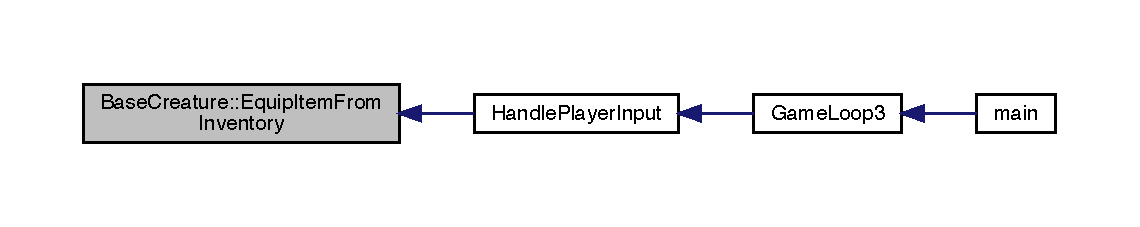
\includegraphics[width=350pt]{d2/d3b/class_base_creature_a637cb7174d9bb9677a21281ff19fb10a_icgraph}
\end{center}
\end{figure}
\mbox{\Hypertarget{class_base_creature_ac04efe1dda147e264998609635baadb6}\label{class_base_creature_ac04efe1dda147e264998609635baadb6}} 
\index{Base\+Creature@{Base\+Creature}!get\+Agility@{get\+Agility}}
\index{get\+Agility@{get\+Agility}!Base\+Creature@{Base\+Creature}}
\subsubsection{\texorpdfstring{get\+Agility()}{getAgility()}}
{\footnotesize\ttfamily short int Base\+Creature\+::get\+Agility (\begin{DoxyParamCaption}{ }\end{DoxyParamCaption}) const}

Here is the caller graph for this function\+:
\nopagebreak
\begin{figure}[H]
\begin{center}
\leavevmode
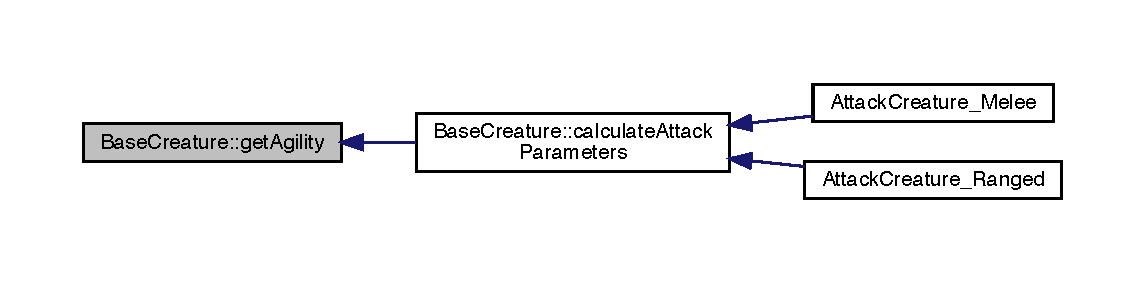
\includegraphics[width=350pt]{d2/d3b/class_base_creature_ac04efe1dda147e264998609635baadb6_icgraph}
\end{center}
\end{figure}
\mbox{\Hypertarget{class_base_creature_ae2fdab903403a68e431baa080f715d3c}\label{class_base_creature_ae2fdab903403a68e431baa080f715d3c}} 
\index{Base\+Creature@{Base\+Creature}!get\+Attacks@{get\+Attacks}}
\index{get\+Attacks@{get\+Attacks}!Base\+Creature@{Base\+Creature}}
\subsubsection{\texorpdfstring{get\+Attacks()}{getAttacks()}}
{\footnotesize\ttfamily std\+::vector$<$ \mbox{\hyperlink{struct_attack_stats}{Attack\+Stats}} $>$ \& Base\+Creature\+::get\+Attacks (\begin{DoxyParamCaption}{ }\end{DoxyParamCaption})}

Here is the caller graph for this function\+:
\nopagebreak
\begin{figure}[H]
\begin{center}
\leavevmode
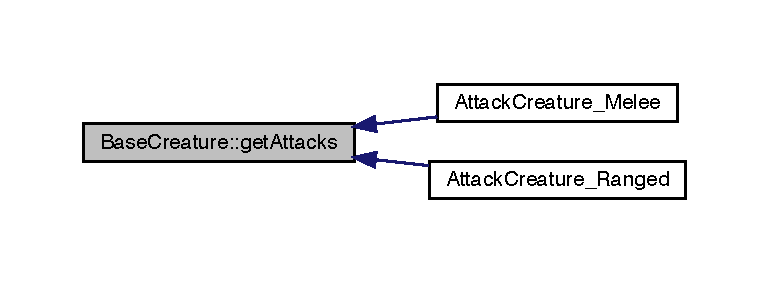
\includegraphics[width=350pt]{d2/d3b/class_base_creature_ae2fdab903403a68e431baa080f715d3c_icgraph}
\end{center}
\end{figure}
\mbox{\Hypertarget{class_base_creature_a4e3864bd12e271718a838ba6c3881f0a}\label{class_base_creature_a4e3864bd12e271718a838ba6c3881f0a}} 
\index{Base\+Creature@{Base\+Creature}!get\+Attack\+Value@{get\+Attack\+Value}}
\index{get\+Attack\+Value@{get\+Attack\+Value}!Base\+Creature@{Base\+Creature}}
\subsubsection{\texorpdfstring{get\+Attack\+Value()}{getAttackValue()}}
{\footnotesize\ttfamily short int Base\+Creature\+::get\+Attack\+Value (\begin{DoxyParamCaption}{ }\end{DoxyParamCaption}) const}

\mbox{\Hypertarget{class_base_creature_a505e70415a3e2db87aac0767498375ff}\label{class_base_creature_a505e70415a3e2db87aac0767498375ff}} 
\index{Base\+Creature@{Base\+Creature}!get\+Inventory@{get\+Inventory}}
\index{get\+Inventory@{get\+Inventory}!Base\+Creature@{Base\+Creature}}
\subsubsection{\texorpdfstring{get\+Inventory()}{getInventory()}}
{\footnotesize\ttfamily std\+::list$<$ \mbox{\hyperlink{class_item}{Item}} $\ast$ $>$ Base\+Creature\+::get\+Inventory (\begin{DoxyParamCaption}{ }\end{DoxyParamCaption})}

Here is the caller graph for this function\+:
\nopagebreak
\begin{figure}[H]
\begin{center}
\leavevmode
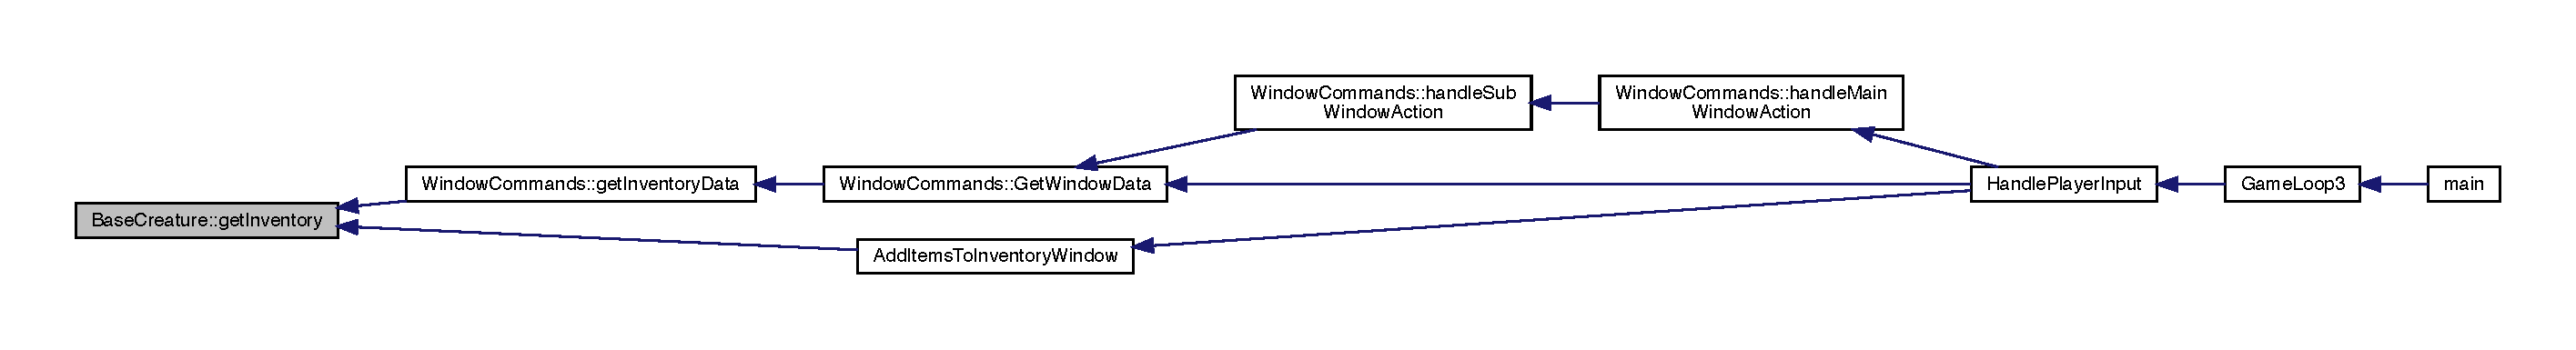
\includegraphics[width=350pt]{d2/d3b/class_base_creature_a505e70415a3e2db87aac0767498375ff_icgraph}
\end{center}
\end{figure}
\mbox{\Hypertarget{class_base_creature_a19f380cccb11f31d10d00de934da1b7f}\label{class_base_creature_a19f380cccb11f31d10d00de934da1b7f}} 
\index{Base\+Creature@{Base\+Creature}!Get\+Item\+Info@{Get\+Item\+Info}}
\index{Get\+Item\+Info@{Get\+Item\+Info}!Base\+Creature@{Base\+Creature}}
\subsubsection{\texorpdfstring{Get\+Item\+Info()}{GetItemInfo()}}
{\footnotesize\ttfamily std\+::string Base\+Creature\+::\+Get\+Item\+Info (\begin{DoxyParamCaption}\item[{int}]{n }\end{DoxyParamCaption})}

\mbox{\Hypertarget{class_base_creature_a7b4f974b77953aea8f4c698e6e21c500}\label{class_base_creature_a7b4f974b77953aea8f4c698e6e21c500}} 
\index{Base\+Creature@{Base\+Creature}!get\+Melee\+Attack\+Value@{get\+Melee\+Attack\+Value}}
\index{get\+Melee\+Attack\+Value@{get\+Melee\+Attack\+Value}!Base\+Creature@{Base\+Creature}}
\subsubsection{\texorpdfstring{get\+Melee\+Attack\+Value()}{getMeleeAttackValue()}}
{\footnotesize\ttfamily short int Base\+Creature\+::get\+Melee\+Attack\+Value (\begin{DoxyParamCaption}{ }\end{DoxyParamCaption}) const}

Here is the caller graph for this function\+:
\nopagebreak
\begin{figure}[H]
\begin{center}
\leavevmode
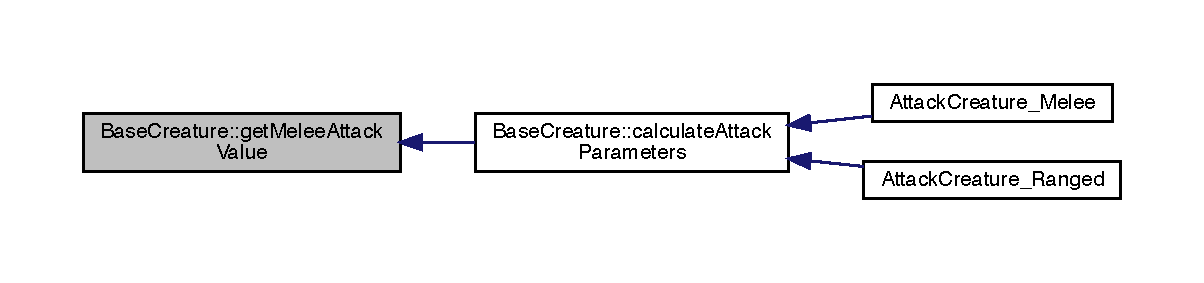
\includegraphics[width=350pt]{d2/d3b/class_base_creature_a7b4f974b77953aea8f4c698e6e21c500_icgraph}
\end{center}
\end{figure}
\mbox{\Hypertarget{class_base_creature_a00ebdc186dd6d3c0ef3c3d1262d4363f}\label{class_base_creature_a00ebdc186dd6d3c0ef3c3d1262d4363f}} 
\index{Base\+Creature@{Base\+Creature}!get\+Position@{get\+Position}}
\index{get\+Position@{get\+Position}!Base\+Creature@{Base\+Creature}}
\subsubsection{\texorpdfstring{get\+Position()}{getPosition()}}
{\footnotesize\ttfamily sf\+::\+Vector2i Base\+Creature\+::get\+Position (\begin{DoxyParamCaption}{ }\end{DoxyParamCaption}) const}

Here is the caller graph for this function\+:
\nopagebreak
\begin{figure}[H]
\begin{center}
\leavevmode
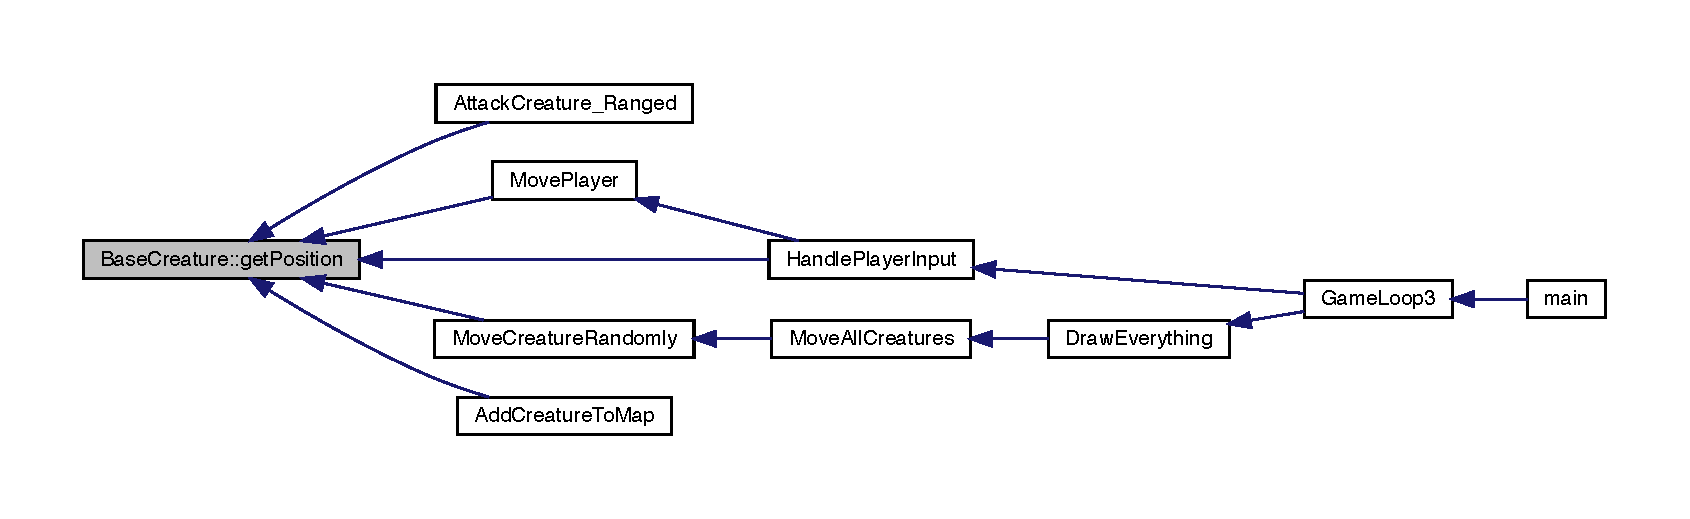
\includegraphics[width=350pt]{d2/d3b/class_base_creature_a00ebdc186dd6d3c0ef3c3d1262d4363f_icgraph}
\end{center}
\end{figure}
\mbox{\Hypertarget{class_base_creature_a58a174420d25df7d0865087586c66a21}\label{class_base_creature_a58a174420d25df7d0865087586c66a21}} 
\index{Base\+Creature@{Base\+Creature}!get\+Ranged\+Attack\+Value@{get\+Ranged\+Attack\+Value}}
\index{get\+Ranged\+Attack\+Value@{get\+Ranged\+Attack\+Value}!Base\+Creature@{Base\+Creature}}
\subsubsection{\texorpdfstring{get\+Ranged\+Attack\+Value()}{getRangedAttackValue()}}
{\footnotesize\ttfamily short int Base\+Creature\+::get\+Ranged\+Attack\+Value (\begin{DoxyParamCaption}{ }\end{DoxyParamCaption}) const}

Here is the caller graph for this function\+:
\nopagebreak
\begin{figure}[H]
\begin{center}
\leavevmode
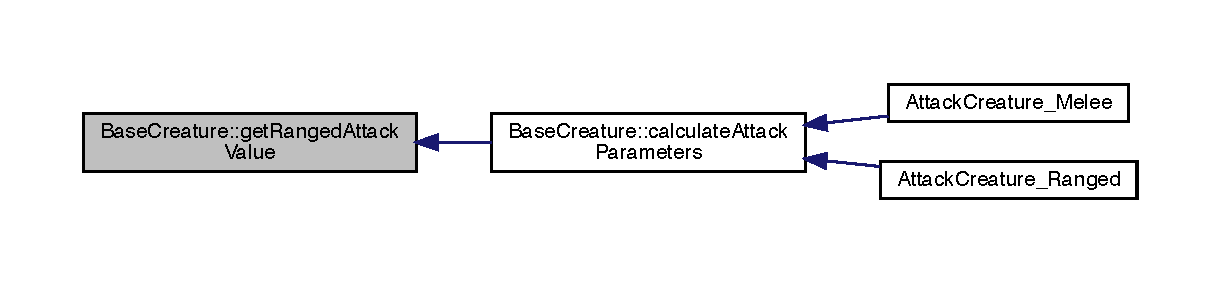
\includegraphics[width=350pt]{d2/d3b/class_base_creature_a58a174420d25df7d0865087586c66a21_icgraph}
\end{center}
\end{figure}
\mbox{\Hypertarget{class_base_creature_a1232a2ecb3199fe79627df912078f24e}\label{class_base_creature_a1232a2ecb3199fe79627df912078f24e}} 
\index{Base\+Creature@{Base\+Creature}!get\+Strength@{get\+Strength}}
\index{get\+Strength@{get\+Strength}!Base\+Creature@{Base\+Creature}}
\subsubsection{\texorpdfstring{get\+Strength()}{getStrength()}}
{\footnotesize\ttfamily short int Base\+Creature\+::get\+Strength (\begin{DoxyParamCaption}{ }\end{DoxyParamCaption}) const}

Here is the caller graph for this function\+:
\nopagebreak
\begin{figure}[H]
\begin{center}
\leavevmode
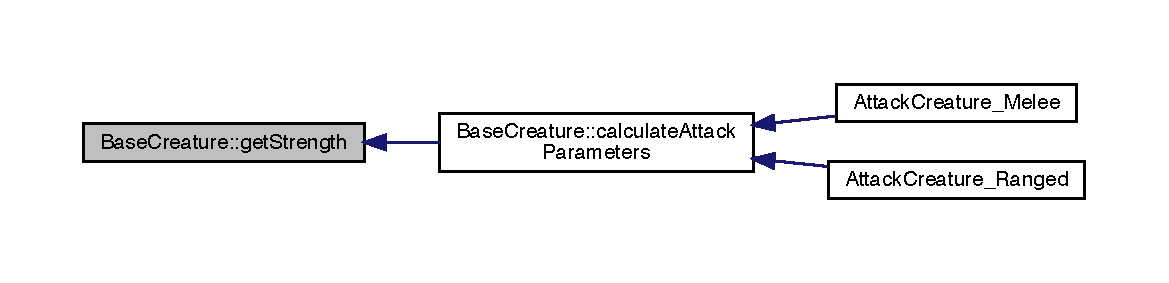
\includegraphics[width=350pt]{d2/d3b/class_base_creature_a1232a2ecb3199fe79627df912078f24e_icgraph}
\end{center}
\end{figure}
\mbox{\Hypertarget{class_base_creature_accab7a878eae0580476b282ce2c556d3}\label{class_base_creature_accab7a878eae0580476b282ce2c556d3}} 
\index{Base\+Creature@{Base\+Creature}!get\+Total\+Health@{get\+Total\+Health}}
\index{get\+Total\+Health@{get\+Total\+Health}!Base\+Creature@{Base\+Creature}}
\subsubsection{\texorpdfstring{get\+Total\+Health()}{getTotalHealth()}}
{\footnotesize\ttfamily int Base\+Creature\+::get\+Total\+Health (\begin{DoxyParamCaption}{ }\end{DoxyParamCaption}) const}

Here is the caller graph for this function\+:
\nopagebreak
\begin{figure}[H]
\begin{center}
\leavevmode
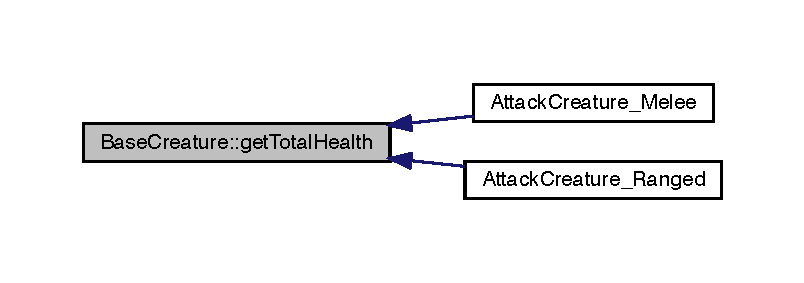
\includegraphics[width=350pt]{d2/d3b/class_base_creature_accab7a878eae0580476b282ce2c556d3_icgraph}
\end{center}
\end{figure}
\mbox{\Hypertarget{class_base_creature_a8a960bc7a7689f5633b1abaa82fa6e95}\label{class_base_creature_a8a960bc7a7689f5633b1abaa82fa6e95}} 
\index{Base\+Creature@{Base\+Creature}!get\+Vision@{get\+Vision}}
\index{get\+Vision@{get\+Vision}!Base\+Creature@{Base\+Creature}}
\subsubsection{\texorpdfstring{get\+Vision()}{getVision()}}
{\footnotesize\ttfamily \mbox{\hyperlink{class_vision}{Vision}} \& Base\+Creature\+::get\+Vision (\begin{DoxyParamCaption}{ }\end{DoxyParamCaption})}

Here is the caller graph for this function\+:
\nopagebreak
\begin{figure}[H]
\begin{center}
\leavevmode
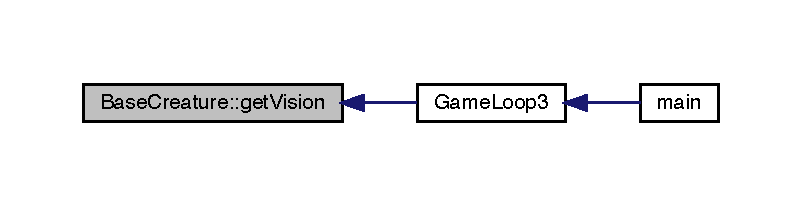
\includegraphics[width=350pt]{d2/d3b/class_base_creature_a8a960bc7a7689f5633b1abaa82fa6e95_icgraph}
\end{center}
\end{figure}
\mbox{\Hypertarget{class_base_creature_af2066b8eb62bf595d30feae6671e4495}\label{class_base_creature_af2066b8eb62bf595d30feae6671e4495}} 
\index{Base\+Creature@{Base\+Creature}!load\+Creature\+Tile@{load\+Creature\+Tile}}
\index{load\+Creature\+Tile@{load\+Creature\+Tile}!Base\+Creature@{Base\+Creature}}
\subsubsection{\texorpdfstring{load\+Creature\+Tile()}{loadCreatureTile()}}
{\footnotesize\ttfamily void Base\+Creature\+::load\+Creature\+Tile (\begin{DoxyParamCaption}\item[{const std\+::string \&}]{tileset,  }\item[{int}]{tile\+X\+Size,  }\item[{int}]{tile\+Y\+Size }\end{DoxyParamCaption})}

Here is the call graph for this function\+:
\nopagebreak
\begin{figure}[H]
\begin{center}
\leavevmode
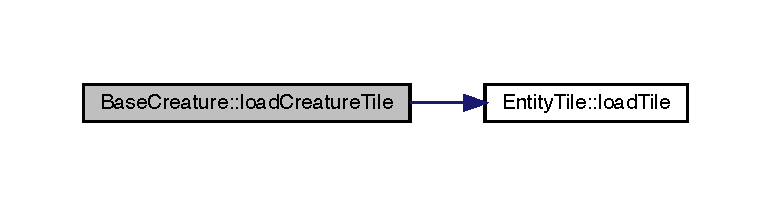
\includegraphics[width=350pt]{d2/d3b/class_base_creature_af2066b8eb62bf595d30feae6671e4495_cgraph}
\end{center}
\end{figure}
Here is the caller graph for this function\+:
\nopagebreak
\begin{figure}[H]
\begin{center}
\leavevmode
\includegraphics[width=350pt]{d2/d3b/class_base_creature_af2066b8eb62bf595d30feae6671e4495_icgraph}
\end{center}
\end{figure}
\mbox{\Hypertarget{class_base_creature_a77f0a7d7c441406c252c3278817454d8}\label{class_base_creature_a77f0a7d7c441406c252c3278817454d8}} 
\index{Base\+Creature@{Base\+Creature}!Move\+Creature@{Move\+Creature}}
\index{Move\+Creature@{Move\+Creature}!Base\+Creature@{Base\+Creature}}
\subsubsection{\texorpdfstring{Move\+Creature()}{MoveCreature()}}
{\footnotesize\ttfamily bool Base\+Creature\+::\+Move\+Creature (\begin{DoxyParamCaption}\item[{int}]{x,  }\item[{int}]{y }\end{DoxyParamCaption})}

Here is the call graph for this function\+:
\nopagebreak
\begin{figure}[H]
\begin{center}
\leavevmode
\includegraphics[width=350pt]{d2/d3b/class_base_creature_a77f0a7d7c441406c252c3278817454d8_cgraph}
\end{center}
\end{figure}
\mbox{\Hypertarget{class_base_creature_a2d45724079ff2eeb6606b222e405e4a8}\label{class_base_creature_a2d45724079ff2eeb6606b222e405e4a8}} 
\index{Base\+Creature@{Base\+Creature}!Pickup\+Item@{Pickup\+Item}}
\index{Pickup\+Item@{Pickup\+Item}!Base\+Creature@{Base\+Creature}}
\subsubsection{\texorpdfstring{Pickup\+Item()}{PickupItem()}}
{\footnotesize\ttfamily void Base\+Creature\+::\+Pickup\+Item (\begin{DoxyParamCaption}\item[{\mbox{\hyperlink{class_map}{Map}} \&}]{map,  }\item[{std\+::list$<$ \mbox{\hyperlink{class_item}{Item}} $\ast$$>$ \&}]{item\+List }\end{DoxyParamCaption})}

Here is the call graph for this function\+:
\nopagebreak
\begin{figure}[H]
\begin{center}
\leavevmode
\includegraphics[width=348pt]{d2/d3b/class_base_creature_a2d45724079ff2eeb6606b222e405e4a8_cgraph}
\end{center}
\end{figure}
Here is the caller graph for this function\+:
\nopagebreak
\begin{figure}[H]
\begin{center}
\leavevmode
\includegraphics[width=350pt]{d2/d3b/class_base_creature_a2d45724079ff2eeb6606b222e405e4a8_icgraph}
\end{center}
\end{figure}
\mbox{\Hypertarget{class_base_creature_ac3d7907a8d8e0967a5881ff180205028}\label{class_base_creature_ac3d7907a8d8e0967a5881ff180205028}} 
\index{Base\+Creature@{Base\+Creature}!Print\+Equipment@{Print\+Equipment}}
\index{Print\+Equipment@{Print\+Equipment}!Base\+Creature@{Base\+Creature}}
\subsubsection{\texorpdfstring{Print\+Equipment()}{PrintEquipment()}}
{\footnotesize\ttfamily void Base\+Creature\+::\+Print\+Equipment (\begin{DoxyParamCaption}{ }\end{DoxyParamCaption})}

\mbox{\Hypertarget{class_base_creature_a097ec44d0b215f75ca75ae69c2bd11be}\label{class_base_creature_a097ec44d0b215f75ca75ae69c2bd11be}} 
\index{Base\+Creature@{Base\+Creature}!Print\+Inventory@{Print\+Inventory}}
\index{Print\+Inventory@{Print\+Inventory}!Base\+Creature@{Base\+Creature}}
\subsubsection{\texorpdfstring{Print\+Inventory()}{PrintInventory()}}
{\footnotesize\ttfamily void Base\+Creature\+::\+Print\+Inventory (\begin{DoxyParamCaption}{ }\end{DoxyParamCaption})}

\mbox{\Hypertarget{class_base_creature_ad6357a6d4456d0b669abd1675efcca30}\label{class_base_creature_ad6357a6d4456d0b669abd1675efcca30}} 
\index{Base\+Creature@{Base\+Creature}!set\+Agility@{set\+Agility}}
\index{set\+Agility@{set\+Agility}!Base\+Creature@{Base\+Creature}}
\subsubsection{\texorpdfstring{set\+Agility()}{setAgility()}}
{\footnotesize\ttfamily void Base\+Creature\+::set\+Agility (\begin{DoxyParamCaption}\item[{int}]{\+\_\+agility }\end{DoxyParamCaption})}

Here is the caller graph for this function\+:
\nopagebreak
\begin{figure}[H]
\begin{center}
\leavevmode
\includegraphics[width=350pt]{d2/d3b/class_base_creature_ad6357a6d4456d0b669abd1675efcca30_icgraph}
\end{center}
\end{figure}
\mbox{\Hypertarget{class_base_creature_a00ffc1ee732a8f0a8921c9cee6842e4d}\label{class_base_creature_a00ffc1ee732a8f0a8921c9cee6842e4d}} 
\index{Base\+Creature@{Base\+Creature}!set\+Position@{set\+Position}}
\index{set\+Position@{set\+Position}!Base\+Creature@{Base\+Creature}}
\subsubsection{\texorpdfstring{set\+Position()}{setPosition()}}
{\footnotesize\ttfamily void Base\+Creature\+::set\+Position (\begin{DoxyParamCaption}\item[{short int}]{x,  }\item[{short int}]{y }\end{DoxyParamCaption})}

Here is the call graph for this function\+:
\nopagebreak
\begin{figure}[H]
\begin{center}
\leavevmode
\includegraphics[width=350pt]{d2/d3b/class_base_creature_a00ffc1ee732a8f0a8921c9cee6842e4d_cgraph}
\end{center}
\end{figure}
Here is the caller graph for this function\+:
\nopagebreak
\begin{figure}[H]
\begin{center}
\leavevmode
\includegraphics[width=350pt]{d2/d3b/class_base_creature_a00ffc1ee732a8f0a8921c9cee6842e4d_icgraph}
\end{center}
\end{figure}
\mbox{\Hypertarget{class_base_creature_a3a2eb318b9c5d849a02884b20e32f83d}\label{class_base_creature_a3a2eb318b9c5d849a02884b20e32f83d}} 
\index{Base\+Creature@{Base\+Creature}!set\+Strength@{set\+Strength}}
\index{set\+Strength@{set\+Strength}!Base\+Creature@{Base\+Creature}}
\subsubsection{\texorpdfstring{set\+Strength()}{setStrength()}}
{\footnotesize\ttfamily void Base\+Creature\+::set\+Strength (\begin{DoxyParamCaption}\item[{int}]{\+\_\+strength }\end{DoxyParamCaption})}

Here is the caller graph for this function\+:
\nopagebreak
\begin{figure}[H]
\begin{center}
\leavevmode
\includegraphics[width=350pt]{d2/d3b/class_base_creature_a3a2eb318b9c5d849a02884b20e32f83d_icgraph}
\end{center}
\end{figure}
\mbox{\Hypertarget{class_base_creature_a82f847585033035597700b071e40611f}\label{class_base_creature_a82f847585033035597700b071e40611f}} 
\index{Base\+Creature@{Base\+Creature}!set\+Total\+Health@{set\+Total\+Health}}
\index{set\+Total\+Health@{set\+Total\+Health}!Base\+Creature@{Base\+Creature}}
\subsubsection{\texorpdfstring{set\+Total\+Health()}{setTotalHealth()}}
{\footnotesize\ttfamily void Base\+Creature\+::set\+Total\+Health (\begin{DoxyParamCaption}\item[{int}]{\+\_\+health }\end{DoxyParamCaption})}

Here is the caller graph for this function\+:
\nopagebreak
\begin{figure}[H]
\begin{center}
\leavevmode
\includegraphics[width=350pt]{d2/d3b/class_base_creature_a82f847585033035597700b071e40611f_icgraph}
\end{center}
\end{figure}
\mbox{\Hypertarget{class_base_creature_ae1cb6e6d01d0c369433fb1fb20803f91}\label{class_base_creature_ae1cb6e6d01d0c369433fb1fb20803f91}} 
\index{Base\+Creature@{Base\+Creature}!set\+Velocity@{set\+Velocity}}
\index{set\+Velocity@{set\+Velocity}!Base\+Creature@{Base\+Creature}}
\subsubsection{\texorpdfstring{set\+Velocity()}{setVelocity()}}
{\footnotesize\ttfamily void Base\+Creature\+::set\+Velocity (\begin{DoxyParamCaption}\item[{int}]{x,  }\item[{int}]{y }\end{DoxyParamCaption})}

\mbox{\Hypertarget{class_base_creature_aaecab78bf5a5a5293079634e813f854f}\label{class_base_creature_aaecab78bf5a5a5293079634e813f854f}} 
\index{Base\+Creature@{Base\+Creature}!Walk\+Path@{Walk\+Path}}
\index{Walk\+Path@{Walk\+Path}!Base\+Creature@{Base\+Creature}}
\subsubsection{\texorpdfstring{Walk\+Path()}{WalkPath()}}
{\footnotesize\ttfamily void Base\+Creature\+::\+Walk\+Path (\begin{DoxyParamCaption}\item[{\mbox{\hyperlink{class_map}{Map}} \&}]{map }\end{DoxyParamCaption})}

Here is the call graph for this function\+:
\nopagebreak
\begin{figure}[H]
\begin{center}
\leavevmode
\includegraphics[width=350pt]{d2/d3b/class_base_creature_aaecab78bf5a5a5293079634e813f854f_cgraph}
\end{center}
\end{figure}
Here is the caller graph for this function\+:
\nopagebreak
\begin{figure}[H]
\begin{center}
\leavevmode
\includegraphics[width=350pt]{d2/d3b/class_base_creature_aaecab78bf5a5a5293079634e813f854f_icgraph}
\end{center}
\end{figure}


\subsection{Member Data Documentation}
\mbox{\Hypertarget{class_base_creature_a23bbce83de8f7be2dfbcec7f5da223ab}\label{class_base_creature_a23bbce83de8f7be2dfbcec7f5da223ab}} 
\index{Base\+Creature@{Base\+Creature}!agility@{agility}}
\index{agility@{agility}!Base\+Creature@{Base\+Creature}}
\subsubsection{\texorpdfstring{agility}{agility}}
{\footnotesize\ttfamily short int Base\+Creature\+::agility\hspace{0.3cm}{\ttfamily [private]}}

\mbox{\Hypertarget{class_base_creature_ab40c21845e4c19538b356bbcb01f7075}\label{class_base_creature_ab40c21845e4c19538b356bbcb01f7075}} 
\index{Base\+Creature@{Base\+Creature}!attacks@{attacks}}
\index{attacks@{attacks}!Base\+Creature@{Base\+Creature}}
\subsubsection{\texorpdfstring{attacks}{attacks}}
{\footnotesize\ttfamily std\+::vector$<$\mbox{\hyperlink{struct_attack_stats}{Attack\+Stats}}$>$ Base\+Creature\+::attacks\hspace{0.3cm}{\ttfamily [private]}}

\mbox{\Hypertarget{class_base_creature_ac5a9c850146fa856dbf7fdd0def635ac}\label{class_base_creature_ac5a9c850146fa856dbf7fdd0def635ac}} 
\index{Base\+Creature@{Base\+Creature}!attack\+Value@{attack\+Value}}
\index{attack\+Value@{attack\+Value}!Base\+Creature@{Base\+Creature}}
\subsubsection{\texorpdfstring{attack\+Value}{attackValue}}
{\footnotesize\ttfamily short int Base\+Creature\+::attack\+Value\hspace{0.3cm}{\ttfamily [private]}}

\mbox{\Hypertarget{class_base_creature_a97e1d629325177b201bdcd43addefd0d}\label{class_base_creature_a97e1d629325177b201bdcd43addefd0d}} 
\index{Base\+Creature@{Base\+Creature}!body@{body}}
\index{body@{body}!Base\+Creature@{Base\+Creature}}
\subsubsection{\texorpdfstring{body}{body}}
{\footnotesize\ttfamily \mbox{\hyperlink{class_creature_body}{Creature\+Body}} Base\+Creature\+::body}

\mbox{\Hypertarget{class_base_creature_aa62b65a4bd43be6e999d9a29a472fffe}\label{class_base_creature_aa62b65a4bd43be6e999d9a29a472fffe}} 
\index{Base\+Creature@{Base\+Creature}!charisma@{charisma}}
\index{charisma@{charisma}!Base\+Creature@{Base\+Creature}}
\subsubsection{\texorpdfstring{charisma}{charisma}}
{\footnotesize\ttfamily short int Base\+Creature\+::charisma\hspace{0.3cm}{\ttfamily [private]}}

\mbox{\Hypertarget{class_base_creature_a15a7a38b2a5bc15d1c3f8eda7e1d835b}\label{class_base_creature_a15a7a38b2a5bc15d1c3f8eda7e1d835b}} 
\index{Base\+Creature@{Base\+Creature}!creature\+Items@{creature\+Items}}
\index{creature\+Items@{creature\+Items}!Base\+Creature@{Base\+Creature}}
\subsubsection{\texorpdfstring{creature\+Items}{creatureItems}}
{\footnotesize\ttfamily std\+::list$<$\mbox{\hyperlink{class_item}{Item}}$\ast$$>$ Base\+Creature\+::creature\+Items\hspace{0.3cm}{\ttfamily [private]}}

\mbox{\Hypertarget{class_base_creature_a35d7353131ee00fe8738ec5a5ebfe231}\label{class_base_creature_a35d7353131ee00fe8738ec5a5ebfe231}} 
\index{Base\+Creature@{Base\+Creature}!creature\+Tile@{creature\+Tile}}
\index{creature\+Tile@{creature\+Tile}!Base\+Creature@{Base\+Creature}}
\subsubsection{\texorpdfstring{creature\+Tile}{creatureTile}}
{\footnotesize\ttfamily \mbox{\hyperlink{class_entity_tile}{Entity\+Tile}} Base\+Creature\+::creature\+Tile}

\mbox{\Hypertarget{class_base_creature_a74bc0648b11f9637b31ad5b76f056740}\label{class_base_creature_a74bc0648b11f9637b31ad5b76f056740}} 
\index{Base\+Creature@{Base\+Creature}!endurance@{endurance}}
\index{endurance@{endurance}!Base\+Creature@{Base\+Creature}}
\subsubsection{\texorpdfstring{endurance}{endurance}}
{\footnotesize\ttfamily short int Base\+Creature\+::endurance\hspace{0.3cm}{\ttfamily [private]}}

\mbox{\Hypertarget{class_base_creature_aa5945485ad5e5974f2600fec2f0a8627}\label{class_base_creature_aa5945485ad5e5974f2600fec2f0a8627}} 
\index{Base\+Creature@{Base\+Creature}!inventory@{inventory}}
\index{inventory@{inventory}!Base\+Creature@{Base\+Creature}}
\subsubsection{\texorpdfstring{inventory}{inventory}}
{\footnotesize\ttfamily \mbox{\hyperlink{class_item_manager}{Item\+Manager}} Base\+Creature\+::inventory}

\mbox{\Hypertarget{class_base_creature_adeb6eed7546d84b1547e8134f582a6c7}\label{class_base_creature_adeb6eed7546d84b1547e8134f582a6c7}} 
\index{Base\+Creature@{Base\+Creature}!is\+Alive@{is\+Alive}}
\index{is\+Alive@{is\+Alive}!Base\+Creature@{Base\+Creature}}
\subsubsection{\texorpdfstring{is\+Alive}{isAlive}}
{\footnotesize\ttfamily bool Base\+Creature\+::is\+Alive\hspace{0.3cm}{\ttfamily [private]}}

\mbox{\Hypertarget{class_base_creature_a8debd17b675db2ac6d944e2ccb314def}\label{class_base_creature_a8debd17b675db2ac6d944e2ccb314def}} 
\index{Base\+Creature@{Base\+Creature}!mind@{mind}}
\index{mind@{mind}!Base\+Creature@{Base\+Creature}}
\subsubsection{\texorpdfstring{mind}{mind}}
{\footnotesize\ttfamily short int Base\+Creature\+::mind\hspace{0.3cm}{\ttfamily [private]}}

\mbox{\Hypertarget{class_base_creature_a846cd45ba49c6496bdcb760651b9aaa8}\label{class_base_creature_a846cd45ba49c6496bdcb760651b9aaa8}} 
\index{Base\+Creature@{Base\+Creature}!move\+Speed@{move\+Speed}}
\index{move\+Speed@{move\+Speed}!Base\+Creature@{Base\+Creature}}
\subsubsection{\texorpdfstring{move\+Speed}{moveSpeed}}
{\footnotesize\ttfamily short int Base\+Creature\+::move\+Speed\hspace{0.3cm}{\ttfamily [private]}}

\mbox{\Hypertarget{class_base_creature_a0e419167e4986de0a4652b8979d66e16}\label{class_base_creature_a0e419167e4986de0a4652b8979d66e16}} 
\index{Base\+Creature@{Base\+Creature}!path@{path}}
\index{path@{path}!Base\+Creature@{Base\+Creature}}
\subsubsection{\texorpdfstring{path}{path}}
{\footnotesize\ttfamily std\+::queue$<$sf\+::\+Vector2i$>$ Base\+Creature\+::path\hspace{0.3cm}{\ttfamily [private]}}

\mbox{\Hypertarget{class_base_creature_ac0aa7211db6bbc4033b0a11e6c34171b}\label{class_base_creature_ac0aa7211db6bbc4033b0a11e6c34171b}} 
\index{Base\+Creature@{Base\+Creature}!position@{position}}
\index{position@{position}!Base\+Creature@{Base\+Creature}}
\subsubsection{\texorpdfstring{position}{position}}
{\footnotesize\ttfamily sf\+::\+Vector2i Base\+Creature\+::position\hspace{0.3cm}{\ttfamily [private]}}

\mbox{\Hypertarget{class_base_creature_a7f325c07376932d6e831dd00a350b806}\label{class_base_creature_a7f325c07376932d6e831dd00a350b806}} 
\index{Base\+Creature@{Base\+Creature}!strength@{strength}}
\index{strength@{strength}!Base\+Creature@{Base\+Creature}}
\subsubsection{\texorpdfstring{strength}{strength}}
{\footnotesize\ttfamily short int Base\+Creature\+::strength\hspace{0.3cm}{\ttfamily [private]}}

\mbox{\Hypertarget{class_base_creature_a727462587a0ec421c549acf8c497de42}\label{class_base_creature_a727462587a0ec421c549acf8c497de42}} 
\index{Base\+Creature@{Base\+Creature}!total\+Health@{total\+Health}}
\index{total\+Health@{total\+Health}!Base\+Creature@{Base\+Creature}}
\subsubsection{\texorpdfstring{total\+Health}{totalHealth}}
{\footnotesize\ttfamily int Base\+Creature\+::total\+Health\hspace{0.3cm}{\ttfamily [private]}}

\mbox{\Hypertarget{class_base_creature_a8433c26fcbcb9bee87c35b15ae2e0814}\label{class_base_creature_a8433c26fcbcb9bee87c35b15ae2e0814}} 
\index{Base\+Creature@{Base\+Creature}!vision@{vision}}
\index{vision@{vision}!Base\+Creature@{Base\+Creature}}
\subsubsection{\texorpdfstring{vision}{vision}}
{\footnotesize\ttfamily \mbox{\hyperlink{class_vision}{Vision}} Base\+Creature\+::vision\hspace{0.3cm}{\ttfamily [private]}}

\mbox{\Hypertarget{class_base_creature_a992cbd3a6be93279f2c933a50eba5000}\label{class_base_creature_a992cbd3a6be93279f2c933a50eba5000}} 
\index{Base\+Creature@{Base\+Creature}!will@{will}}
\index{will@{will}!Base\+Creature@{Base\+Creature}}
\subsubsection{\texorpdfstring{will}{will}}
{\footnotesize\ttfamily short int Base\+Creature\+::will\hspace{0.3cm}{\ttfamily [private]}}



The documentation for this class was generated from the following files\+:\begin{DoxyCompactItemize}
\item 
/\+Users/\+Afromullet/\+Documents/\+S\+F\+M\+L/\+Colony2/\+Colony/\+Creature/\mbox{\hyperlink{_base_creature_8hpp}{Base\+Creature.\+hpp}}\item 
/\+Users/\+Afromullet/\+Documents/\+S\+F\+M\+L/\+Colony2/\+Colony/\+Creature/\mbox{\hyperlink{_base_creature_8cpp}{Base\+Creature.\+cpp}}\end{DoxyCompactItemize}

\hypertarget{class_biome}{}\section{Biome Class Reference}
\label{class_biome}\index{Biome@{Biome}}


{\ttfamily \#include $<$Biomes.\+hpp$>$}



Collaboration diagram for Biome\+:
\nopagebreak
\begin{figure}[H]
\begin{center}
\leavevmode
\includegraphics[width=207pt]{d8/d78/class_biome__coll__graph}
\end{center}
\end{figure}
\subsection*{Public Member Functions}
\begin{DoxyCompactItemize}
\item 
bool \mbox{\hyperlink{class_biome_ab30d25f0400f31071794964de3224b6b}{operator==}} (const \mbox{\hyperlink{class_biome}{Biome}} \&other) const
\item 
bool \mbox{\hyperlink{class_biome_a5f619965ed1bf4b1f7423cbb69be3559}{operator!=}} (const \mbox{\hyperlink{class_biome}{Biome}} \&other) const
\item 
void \mbox{\hyperlink{class_biome_a5a66500c836cefef0f6cf47af93fe3df}{operator=}} (const \mbox{\hyperlink{class_biome}{Biome}} \&other)
\item 
\mbox{\hyperlink{class_biome_aa340fc9737f1f60fe4aa99f5d4d5c726}{Biome}} ()
\item 
\mbox{\hyperlink{class_biome_a6145de7d30bcbef4b6042ee456f88f16}{Biome}} (const \mbox{\hyperlink{class_biome}{Biome}} \&biome)
\item 
void \mbox{\hyperlink{class_biome_acc568302ef1e66d443d2e43d94b36a10}{set\+Temperature\+Limits}} (float \+\_\+low\+Temp, float \+\_\+high\+Temp)
\item 
void \mbox{\hyperlink{class_biome_afb3047918646d9d7717b74091efa378b}{set\+Biome}} (\mbox{\hyperlink{_enum_types_8hpp_a5c2255009cd01c90cf68245e6f453d1c}{en\+Biomes}} \+\_\+\+En\+Biome)
\item 
void \mbox{\hyperlink{class_biome_a4b702cd936eb35364493be9e3e3c4166}{set\+Biome\+Name}} (std\+::string \+\_\+name)
\item 
void \mbox{\hyperlink{class_biome_a73164a278cfd1c3c6cf52a6b006034e0}{set\+Current\+Temp}} (float \+\_\+current\+Temp)
\item 
void \mbox{\hyperlink{class_biome_adbe071450d7411ddd3f886b1c84c2029}{set\+Vegetation\+Level}} (float level)
\item 
void \mbox{\hyperlink{class_biome_adb9f34f853f233464a33a5dfbb2ccbee}{set\+Treelevel}} (float level)
\item 
void \mbox{\hyperlink{class_biome_afe05b01787008c396ccad3ffd7e6d6cd}{set\+Wildlife\+Level}} (float level)
\item 
float \mbox{\hyperlink{class_biome_a198f0bb873cce52c8e62df2cf0282e84}{get\+Low\+Temp}} ()
\item 
float \mbox{\hyperlink{class_biome_afc882c431129cdaae8109ad5dcc8267e}{get\+High\+Temp}} ()
\item 
float \mbox{\hyperlink{class_biome_ac347b6eeccd189054af58983acd62ea3}{get\+Current\+Temp}} ()
\item 
float \mbox{\hyperlink{class_biome_aaa9ebdc0dde9b6737da890299a7b5ea4}{get\+Wildlife\+Level}} ()
\item 
float \mbox{\hyperlink{class_biome_a93767d0c392cdef6c3c527a4dbe38efd}{get\+Vegetation\+Level}} ()
\item 
float \mbox{\hyperlink{class_biome_a052e0b1b6a6167f3e076a64a59487172}{get\+Tree\+Level}} ()
\item 
std\+::string \mbox{\hyperlink{class_biome_ad3cbf2a1fcdea543a2104fde28766f90}{get\+Biome\+Name}} ()
\item 
\mbox{\hyperlink{_enum_types_8hpp_a5c2255009cd01c90cf68245e6f453d1c}{en\+Biomes}} \mbox{\hyperlink{class_biome_aed98ff023d5563e1ca0309180064fbc4}{get\+Biome}} ()
\end{DoxyCompactItemize}
\subsection*{Private Attributes}
\begin{DoxyCompactItemize}
\item 
float \mbox{\hyperlink{class_biome_afe7165774528de18876c2df0b08faa9d}{low\+Temp}}
\item 
float \mbox{\hyperlink{class_biome_a389c810fbb09eea1fa5c4553ac976c77}{high\+Temp}}
\item 
float \mbox{\hyperlink{class_biome_a80ffc723aed56c5d9390a45e22a7742c}{current\+Temp}}
\item 
float \mbox{\hyperlink{class_biome_af2e689d891f991d1ec7abedb2d8cbfe6}{vegetation\+Level}}
\item 
float \mbox{\hyperlink{class_biome_aab11a193d913aeccf5a5d4d8af6ccd05}{tree\+Level}}
\item 
float \mbox{\hyperlink{class_biome_a4568b5f65ed8b774ef37d1126bb5ecd1}{wildlife\+Level}}
\item 
\mbox{\hyperlink{_enum_types_8hpp_a5c2255009cd01c90cf68245e6f453d1c}{en\+Biomes}} \mbox{\hyperlink{class_biome_a9171c1298078010a780475f5c0ab9d58}{En\+Biome}}
\item 
std\+::string \mbox{\hyperlink{class_biome_a45d0a14ac780f5a5a0215df8be24e8cf}{name}}
\end{DoxyCompactItemize}


\subsection{Constructor \& Destructor Documentation}
\mbox{\Hypertarget{class_biome_aa340fc9737f1f60fe4aa99f5d4d5c726}\label{class_biome_aa340fc9737f1f60fe4aa99f5d4d5c726}} 
\index{Biome@{Biome}!Biome@{Biome}}
\index{Biome@{Biome}!Biome@{Biome}}
\subsubsection{\texorpdfstring{Biome()}{Biome()}\hspace{0.1cm}{\footnotesize\ttfamily [1/2]}}
{\footnotesize\ttfamily Biome\+::\+Biome (\begin{DoxyParamCaption}{ }\end{DoxyParamCaption})}

\mbox{\Hypertarget{class_biome_a6145de7d30bcbef4b6042ee456f88f16}\label{class_biome_a6145de7d30bcbef4b6042ee456f88f16}} 
\index{Biome@{Biome}!Biome@{Biome}}
\index{Biome@{Biome}!Biome@{Biome}}
\subsubsection{\texorpdfstring{Biome()}{Biome()}\hspace{0.1cm}{\footnotesize\ttfamily [2/2]}}
{\footnotesize\ttfamily Biome\+::\+Biome (\begin{DoxyParamCaption}\item[{const \mbox{\hyperlink{class_biome}{Biome}} \&}]{biome }\end{DoxyParamCaption})}



\subsection{Member Function Documentation}
\mbox{\Hypertarget{class_biome_aed98ff023d5563e1ca0309180064fbc4}\label{class_biome_aed98ff023d5563e1ca0309180064fbc4}} 
\index{Biome@{Biome}!get\+Biome@{get\+Biome}}
\index{get\+Biome@{get\+Biome}!Biome@{Biome}}
\subsubsection{\texorpdfstring{get\+Biome()}{getBiome()}}
{\footnotesize\ttfamily \mbox{\hyperlink{_enum_types_8hpp_a5c2255009cd01c90cf68245e6f453d1c}{en\+Biomes}} Biome\+::get\+Biome (\begin{DoxyParamCaption}{ }\end{DoxyParamCaption})}

\mbox{\Hypertarget{class_biome_ad3cbf2a1fcdea543a2104fde28766f90}\label{class_biome_ad3cbf2a1fcdea543a2104fde28766f90}} 
\index{Biome@{Biome}!get\+Biome\+Name@{get\+Biome\+Name}}
\index{get\+Biome\+Name@{get\+Biome\+Name}!Biome@{Biome}}
\subsubsection{\texorpdfstring{get\+Biome\+Name()}{getBiomeName()}}
{\footnotesize\ttfamily std\+::string Biome\+::get\+Biome\+Name (\begin{DoxyParamCaption}{ }\end{DoxyParamCaption})}

\mbox{\Hypertarget{class_biome_ac347b6eeccd189054af58983acd62ea3}\label{class_biome_ac347b6eeccd189054af58983acd62ea3}} 
\index{Biome@{Biome}!get\+Current\+Temp@{get\+Current\+Temp}}
\index{get\+Current\+Temp@{get\+Current\+Temp}!Biome@{Biome}}
\subsubsection{\texorpdfstring{get\+Current\+Temp()}{getCurrentTemp()}}
{\footnotesize\ttfamily float Biome\+::get\+Current\+Temp (\begin{DoxyParamCaption}{ }\end{DoxyParamCaption})}

\mbox{\Hypertarget{class_biome_afc882c431129cdaae8109ad5dcc8267e}\label{class_biome_afc882c431129cdaae8109ad5dcc8267e}} 
\index{Biome@{Biome}!get\+High\+Temp@{get\+High\+Temp}}
\index{get\+High\+Temp@{get\+High\+Temp}!Biome@{Biome}}
\subsubsection{\texorpdfstring{get\+High\+Temp()}{getHighTemp()}}
{\footnotesize\ttfamily float Biome\+::get\+High\+Temp (\begin{DoxyParamCaption}{ }\end{DoxyParamCaption})}

Here is the caller graph for this function\+:
\nopagebreak
\begin{figure}[H]
\begin{center}
\leavevmode
\includegraphics[width=350pt]{d6/dd0/class_biome_afc882c431129cdaae8109ad5dcc8267e_icgraph}
\end{center}
\end{figure}
\mbox{\Hypertarget{class_biome_a198f0bb873cce52c8e62df2cf0282e84}\label{class_biome_a198f0bb873cce52c8e62df2cf0282e84}} 
\index{Biome@{Biome}!get\+Low\+Temp@{get\+Low\+Temp}}
\index{get\+Low\+Temp@{get\+Low\+Temp}!Biome@{Biome}}
\subsubsection{\texorpdfstring{get\+Low\+Temp()}{getLowTemp()}}
{\footnotesize\ttfamily float Biome\+::get\+Low\+Temp (\begin{DoxyParamCaption}{ }\end{DoxyParamCaption})}

Here is the caller graph for this function\+:
\nopagebreak
\begin{figure}[H]
\begin{center}
\leavevmode
\includegraphics[width=350pt]{d6/dd0/class_biome_a198f0bb873cce52c8e62df2cf0282e84_icgraph}
\end{center}
\end{figure}
\mbox{\Hypertarget{class_biome_a052e0b1b6a6167f3e076a64a59487172}\label{class_biome_a052e0b1b6a6167f3e076a64a59487172}} 
\index{Biome@{Biome}!get\+Tree\+Level@{get\+Tree\+Level}}
\index{get\+Tree\+Level@{get\+Tree\+Level}!Biome@{Biome}}
\subsubsection{\texorpdfstring{get\+Tree\+Level()}{getTreeLevel()}}
{\footnotesize\ttfamily float Biome\+::get\+Tree\+Level (\begin{DoxyParamCaption}{ }\end{DoxyParamCaption})}

\mbox{\Hypertarget{class_biome_a93767d0c392cdef6c3c527a4dbe38efd}\label{class_biome_a93767d0c392cdef6c3c527a4dbe38efd}} 
\index{Biome@{Biome}!get\+Vegetation\+Level@{get\+Vegetation\+Level}}
\index{get\+Vegetation\+Level@{get\+Vegetation\+Level}!Biome@{Biome}}
\subsubsection{\texorpdfstring{get\+Vegetation\+Level()}{getVegetationLevel()}}
{\footnotesize\ttfamily float Biome\+::get\+Vegetation\+Level (\begin{DoxyParamCaption}{ }\end{DoxyParamCaption})}

\mbox{\Hypertarget{class_biome_aaa9ebdc0dde9b6737da890299a7b5ea4}\label{class_biome_aaa9ebdc0dde9b6737da890299a7b5ea4}} 
\index{Biome@{Biome}!get\+Wildlife\+Level@{get\+Wildlife\+Level}}
\index{get\+Wildlife\+Level@{get\+Wildlife\+Level}!Biome@{Biome}}
\subsubsection{\texorpdfstring{get\+Wildlife\+Level()}{getWildlifeLevel()}}
{\footnotesize\ttfamily float Biome\+::get\+Wildlife\+Level (\begin{DoxyParamCaption}{ }\end{DoxyParamCaption})}

\mbox{\Hypertarget{class_biome_a5f619965ed1bf4b1f7423cbb69be3559}\label{class_biome_a5f619965ed1bf4b1f7423cbb69be3559}} 
\index{Biome@{Biome}!operator"!=@{operator"!=}}
\index{operator"!=@{operator"!=}!Biome@{Biome}}
\subsubsection{\texorpdfstring{operator"!=()}{operator!=()}}
{\footnotesize\ttfamily bool Biome\+::operator!= (\begin{DoxyParamCaption}\item[{const \mbox{\hyperlink{class_biome}{Biome}} \&}]{other }\end{DoxyParamCaption}) const}

\mbox{\Hypertarget{class_biome_a5a66500c836cefef0f6cf47af93fe3df}\label{class_biome_a5a66500c836cefef0f6cf47af93fe3df}} 
\index{Biome@{Biome}!operator=@{operator=}}
\index{operator=@{operator=}!Biome@{Biome}}
\subsubsection{\texorpdfstring{operator=()}{operator=()}}
{\footnotesize\ttfamily void Biome\+::operator= (\begin{DoxyParamCaption}\item[{const \mbox{\hyperlink{class_biome}{Biome}} \&}]{other }\end{DoxyParamCaption})}

\mbox{\Hypertarget{class_biome_ab30d25f0400f31071794964de3224b6b}\label{class_biome_ab30d25f0400f31071794964de3224b6b}} 
\index{Biome@{Biome}!operator==@{operator==}}
\index{operator==@{operator==}!Biome@{Biome}}
\subsubsection{\texorpdfstring{operator==()}{operator==()}}
{\footnotesize\ttfamily bool Biome\+::operator== (\begin{DoxyParamCaption}\item[{const \mbox{\hyperlink{class_biome}{Biome}} \&}]{other }\end{DoxyParamCaption}) const}

\mbox{\Hypertarget{class_biome_afb3047918646d9d7717b74091efa378b}\label{class_biome_afb3047918646d9d7717b74091efa378b}} 
\index{Biome@{Biome}!set\+Biome@{set\+Biome}}
\index{set\+Biome@{set\+Biome}!Biome@{Biome}}
\subsubsection{\texorpdfstring{set\+Biome()}{setBiome()}}
{\footnotesize\ttfamily void Biome\+::set\+Biome (\begin{DoxyParamCaption}\item[{\mbox{\hyperlink{_enum_types_8hpp_a5c2255009cd01c90cf68245e6f453d1c}{en\+Biomes}}}]{\+\_\+\+En\+Biome }\end{DoxyParamCaption})}

\mbox{\Hypertarget{class_biome_a4b702cd936eb35364493be9e3e3c4166}\label{class_biome_a4b702cd936eb35364493be9e3e3c4166}} 
\index{Biome@{Biome}!set\+Biome\+Name@{set\+Biome\+Name}}
\index{set\+Biome\+Name@{set\+Biome\+Name}!Biome@{Biome}}
\subsubsection{\texorpdfstring{set\+Biome\+Name()}{setBiomeName()}}
{\footnotesize\ttfamily void Biome\+::set\+Biome\+Name (\begin{DoxyParamCaption}\item[{std\+::string}]{\+\_\+name }\end{DoxyParamCaption})}

Here is the caller graph for this function\+:
\nopagebreak
\begin{figure}[H]
\begin{center}
\leavevmode
\includegraphics[width=350pt]{d6/dd0/class_biome_a4b702cd936eb35364493be9e3e3c4166_icgraph}
\end{center}
\end{figure}
\mbox{\Hypertarget{class_biome_a73164a278cfd1c3c6cf52a6b006034e0}\label{class_biome_a73164a278cfd1c3c6cf52a6b006034e0}} 
\index{Biome@{Biome}!set\+Current\+Temp@{set\+Current\+Temp}}
\index{set\+Current\+Temp@{set\+Current\+Temp}!Biome@{Biome}}
\subsubsection{\texorpdfstring{set\+Current\+Temp()}{setCurrentTemp()}}
{\footnotesize\ttfamily void Biome\+::set\+Current\+Temp (\begin{DoxyParamCaption}\item[{float}]{\+\_\+current\+Temp }\end{DoxyParamCaption})}

Here is the caller graph for this function\+:
\nopagebreak
\begin{figure}[H]
\begin{center}
\leavevmode
\includegraphics[width=350pt]{d6/dd0/class_biome_a73164a278cfd1c3c6cf52a6b006034e0_icgraph}
\end{center}
\end{figure}
\mbox{\Hypertarget{class_biome_acc568302ef1e66d443d2e43d94b36a10}\label{class_biome_acc568302ef1e66d443d2e43d94b36a10}} 
\index{Biome@{Biome}!set\+Temperature\+Limits@{set\+Temperature\+Limits}}
\index{set\+Temperature\+Limits@{set\+Temperature\+Limits}!Biome@{Biome}}
\subsubsection{\texorpdfstring{set\+Temperature\+Limits()}{setTemperatureLimits()}}
{\footnotesize\ttfamily void Biome\+::set\+Temperature\+Limits (\begin{DoxyParamCaption}\item[{float}]{\+\_\+low\+Temp,  }\item[{float}]{\+\_\+high\+Temp }\end{DoxyParamCaption})}

Here is the caller graph for this function\+:
\nopagebreak
\begin{figure}[H]
\begin{center}
\leavevmode
\includegraphics[width=350pt]{d6/dd0/class_biome_acc568302ef1e66d443d2e43d94b36a10_icgraph}
\end{center}
\end{figure}
\mbox{\Hypertarget{class_biome_adb9f34f853f233464a33a5dfbb2ccbee}\label{class_biome_adb9f34f853f233464a33a5dfbb2ccbee}} 
\index{Biome@{Biome}!set\+Treelevel@{set\+Treelevel}}
\index{set\+Treelevel@{set\+Treelevel}!Biome@{Biome}}
\subsubsection{\texorpdfstring{set\+Treelevel()}{setTreelevel()}}
{\footnotesize\ttfamily void Biome\+::set\+Treelevel (\begin{DoxyParamCaption}\item[{float}]{level }\end{DoxyParamCaption})}

Here is the caller graph for this function\+:
\nopagebreak
\begin{figure}[H]
\begin{center}
\leavevmode
\includegraphics[width=350pt]{d6/dd0/class_biome_adb9f34f853f233464a33a5dfbb2ccbee_icgraph}
\end{center}
\end{figure}
\mbox{\Hypertarget{class_biome_adbe071450d7411ddd3f886b1c84c2029}\label{class_biome_adbe071450d7411ddd3f886b1c84c2029}} 
\index{Biome@{Biome}!set\+Vegetation\+Level@{set\+Vegetation\+Level}}
\index{set\+Vegetation\+Level@{set\+Vegetation\+Level}!Biome@{Biome}}
\subsubsection{\texorpdfstring{set\+Vegetation\+Level()}{setVegetationLevel()}}
{\footnotesize\ttfamily void Biome\+::set\+Vegetation\+Level (\begin{DoxyParamCaption}\item[{float}]{level }\end{DoxyParamCaption})}

Here is the caller graph for this function\+:
\nopagebreak
\begin{figure}[H]
\begin{center}
\leavevmode
\includegraphics[width=350pt]{d6/dd0/class_biome_adbe071450d7411ddd3f886b1c84c2029_icgraph}
\end{center}
\end{figure}
\mbox{\Hypertarget{class_biome_afe05b01787008c396ccad3ffd7e6d6cd}\label{class_biome_afe05b01787008c396ccad3ffd7e6d6cd}} 
\index{Biome@{Biome}!set\+Wildlife\+Level@{set\+Wildlife\+Level}}
\index{set\+Wildlife\+Level@{set\+Wildlife\+Level}!Biome@{Biome}}
\subsubsection{\texorpdfstring{set\+Wildlife\+Level()}{setWildlifeLevel()}}
{\footnotesize\ttfamily void Biome\+::set\+Wildlife\+Level (\begin{DoxyParamCaption}\item[{float}]{level }\end{DoxyParamCaption})}

Here is the caller graph for this function\+:
\nopagebreak
\begin{figure}[H]
\begin{center}
\leavevmode
\includegraphics[width=350pt]{d6/dd0/class_biome_afe05b01787008c396ccad3ffd7e6d6cd_icgraph}
\end{center}
\end{figure}


\subsection{Member Data Documentation}
\mbox{\Hypertarget{class_biome_a80ffc723aed56c5d9390a45e22a7742c}\label{class_biome_a80ffc723aed56c5d9390a45e22a7742c}} 
\index{Biome@{Biome}!current\+Temp@{current\+Temp}}
\index{current\+Temp@{current\+Temp}!Biome@{Biome}}
\subsubsection{\texorpdfstring{current\+Temp}{currentTemp}}
{\footnotesize\ttfamily float Biome\+::current\+Temp\hspace{0.3cm}{\ttfamily [private]}}

\mbox{\Hypertarget{class_biome_a9171c1298078010a780475f5c0ab9d58}\label{class_biome_a9171c1298078010a780475f5c0ab9d58}} 
\index{Biome@{Biome}!En\+Biome@{En\+Biome}}
\index{En\+Biome@{En\+Biome}!Biome@{Biome}}
\subsubsection{\texorpdfstring{En\+Biome}{EnBiome}}
{\footnotesize\ttfamily \mbox{\hyperlink{_enum_types_8hpp_a5c2255009cd01c90cf68245e6f453d1c}{en\+Biomes}} Biome\+::\+En\+Biome\hspace{0.3cm}{\ttfamily [private]}}

\mbox{\Hypertarget{class_biome_a389c810fbb09eea1fa5c4553ac976c77}\label{class_biome_a389c810fbb09eea1fa5c4553ac976c77}} 
\index{Biome@{Biome}!high\+Temp@{high\+Temp}}
\index{high\+Temp@{high\+Temp}!Biome@{Biome}}
\subsubsection{\texorpdfstring{high\+Temp}{highTemp}}
{\footnotesize\ttfamily float Biome\+::high\+Temp\hspace{0.3cm}{\ttfamily [private]}}

\mbox{\Hypertarget{class_biome_afe7165774528de18876c2df0b08faa9d}\label{class_biome_afe7165774528de18876c2df0b08faa9d}} 
\index{Biome@{Biome}!low\+Temp@{low\+Temp}}
\index{low\+Temp@{low\+Temp}!Biome@{Biome}}
\subsubsection{\texorpdfstring{low\+Temp}{lowTemp}}
{\footnotesize\ttfamily float Biome\+::low\+Temp\hspace{0.3cm}{\ttfamily [private]}}

\mbox{\Hypertarget{class_biome_a45d0a14ac780f5a5a0215df8be24e8cf}\label{class_biome_a45d0a14ac780f5a5a0215df8be24e8cf}} 
\index{Biome@{Biome}!name@{name}}
\index{name@{name}!Biome@{Biome}}
\subsubsection{\texorpdfstring{name}{name}}
{\footnotesize\ttfamily std\+::string Biome\+::name\hspace{0.3cm}{\ttfamily [private]}}

\mbox{\Hypertarget{class_biome_aab11a193d913aeccf5a5d4d8af6ccd05}\label{class_biome_aab11a193d913aeccf5a5d4d8af6ccd05}} 
\index{Biome@{Biome}!tree\+Level@{tree\+Level}}
\index{tree\+Level@{tree\+Level}!Biome@{Biome}}
\subsubsection{\texorpdfstring{tree\+Level}{treeLevel}}
{\footnotesize\ttfamily float Biome\+::tree\+Level\hspace{0.3cm}{\ttfamily [private]}}

\mbox{\Hypertarget{class_biome_af2e689d891f991d1ec7abedb2d8cbfe6}\label{class_biome_af2e689d891f991d1ec7abedb2d8cbfe6}} 
\index{Biome@{Biome}!vegetation\+Level@{vegetation\+Level}}
\index{vegetation\+Level@{vegetation\+Level}!Biome@{Biome}}
\subsubsection{\texorpdfstring{vegetation\+Level}{vegetationLevel}}
{\footnotesize\ttfamily float Biome\+::vegetation\+Level\hspace{0.3cm}{\ttfamily [private]}}

\mbox{\Hypertarget{class_biome_a4568b5f65ed8b774ef37d1126bb5ecd1}\label{class_biome_a4568b5f65ed8b774ef37d1126bb5ecd1}} 
\index{Biome@{Biome}!wildlife\+Level@{wildlife\+Level}}
\index{wildlife\+Level@{wildlife\+Level}!Biome@{Biome}}
\subsubsection{\texorpdfstring{wildlife\+Level}{wildlifeLevel}}
{\footnotesize\ttfamily float Biome\+::wildlife\+Level\hspace{0.3cm}{\ttfamily [private]}}



The documentation for this class was generated from the following files\+:\begin{DoxyCompactItemize}
\item 
/\+Users/\+Afromullet/\+Documents/\+S\+F\+M\+L/\+Colony2/\+Colony/\+Map\+Components/\+Biome/\mbox{\hyperlink{_biomes_8hpp}{Biomes.\+hpp}}\item 
/\+Users/\+Afromullet/\+Documents/\+S\+F\+M\+L/\+Colony2/\+Colony/\+Map\+Components/\+Biome/\mbox{\hyperlink{_biomes_8cpp}{Biomes.\+cpp}}\end{DoxyCompactItemize}

\hypertarget{class_body_part}{}\section{Body\+Part Class Reference}
\label{class_body_part}\index{Body\+Part@{Body\+Part}}


{\ttfamily \#include $<$Body\+Part.\+hpp$>$}



Collaboration diagram for Body\+Part\+:
\nopagebreak
\begin{figure}[H]
\begin{center}
\leavevmode
\includegraphics[height=550pt]{df/dc2/class_body_part__coll__graph}
\end{center}
\end{figure}
\subsection*{Public Member Functions}
\begin{DoxyCompactItemize}
\item 
bool \mbox{\hyperlink{class_body_part_a9fa30957d2740122ef8d3bf1905c2dda}{operator==}} (\mbox{\hyperlink{class_body_part}{Body\+Part}} \&other) const
\item 
bool \mbox{\hyperlink{class_body_part_aa5df801cc11333d0adeaa5235c70bc7c}{operator!=}} (\mbox{\hyperlink{class_body_part}{Body\+Part}} \&other) const
\item 
void \mbox{\hyperlink{class_body_part_af4df2320cea8651ff589a57778ba4eee}{operator=}} (const \mbox{\hyperlink{class_body_part}{Body\+Part}} \&other)
\item 
\mbox{\hyperlink{class_body_part_a9599eb919a1223d5597f85fedd74085a}{Body\+Part}} ()
\item 
\mbox{\hyperlink{class_body_part_a84e12a892612a548a4fd605835290557}{Body\+Part}} (bool \+\_\+can\+Hold\+Weapon, bool \+\_\+can\+Hold\+Armor, bool \+\_\+can\+Interact, bool \+\_\+can\+Move\+Creature, std\+::string \+\_\+body\+Part\+Name, int \+\_\+health)
\item 
\mbox{\hyperlink{class_body_part_ac09038a5c7837d63f5f2b97747a88854}{Body\+Part}} (std\+::string bptoken, std\+::string bpname)
\item 
\mbox{\hyperlink{class_body_part_a605504c8f1ce6c8977c409c052b82633}{Body\+Part}} (const \mbox{\hyperlink{class_body_part}{Body\+Part}} \&other)
\item 
void \mbox{\hyperlink{class_body_part_aa12ae5563a19cabd664731bbba3c7ea6}{Equip\+Armor}} (\mbox{\hyperlink{class_item}{Item}} $\ast$item)
\item 
void \mbox{\hyperlink{class_body_part_a651b65c40c95ecad5a8388736d6cc73a}{Equip\+Armor}} (\mbox{\hyperlink{class_armor}{Armor}} val)
\item 
void \mbox{\hyperlink{class_body_part_a6af5139c60c7b96bff6d8768c9ef8f22}{Equip\+Weapon}} (\mbox{\hyperlink{class_item}{Item}} $\ast$item)
\item 
std\+::vector$<$ \mbox{\hyperlink{struct_applied_force_effect}{Applied\+Force\+Effect}} $>$ \mbox{\hyperlink{class_body_part_aed6e734467a8cd25b4be8bc18edc9033}{Apply\+Attack}} (\mbox{\hyperlink{struct_attack_stats}{Attack\+Stats}} params)
\item 
void \mbox{\hyperlink{class_body_part_ae8ee6c320cd7ad82ec2c674357d16b80}{Apply\+Damage}} (int damage)
\item 
void \mbox{\hyperlink{class_body_part_a59d24b904169031b36cef2f4ba2847f1}{Show\+Wounds}} ()
\item 
void \mbox{\hyperlink{class_body_part_aad10894946e0dc672d9fbaecae496cc9}{Clear\+Wounds}} ()
\item 
void \mbox{\hyperlink{class_body_part_a089afe1bbd06d3fc84a9870ec173883c}{set\+Armor}} (\mbox{\hyperlink{class_armor}{Armor}} val)
\item 
void \mbox{\hyperlink{class_body_part_a12897c5566d467977f7bbbe39665c4f5}{set\+Weapon}} (\mbox{\hyperlink{class_weapon}{Weapon}} val)
\item 
void \mbox{\hyperlink{class_body_part_aca91d2ed2644a952b437a3e1f5155318}{set\+Health}} (int val)
\item 
void \mbox{\hyperlink{class_body_part_a042e07259ce197a1077fe36660332a33}{set\+Armor\+Material\+Effects}} (\mbox{\hyperlink{struct_applied_force_effect}{Applied\+Force\+Effect}} val)
\item 
void \mbox{\hyperlink{class_body_part_a15d3ae087969dc50e7db331c73bd346b}{set\+Has\+Weapon}} (bool val)
\item 
void \mbox{\hyperlink{class_body_part_ac4d2365cc57317596096db2b56f52c91}{set\+ID}} (int val)
\item 
void \mbox{\hyperlink{class_body_part_afe0684374c38122fe9316bedff8742dc}{set\+Body\+Part\+Token}} (std\+::string val)
\item 
void \mbox{\hyperlink{class_body_part_acae2236af2e131dfb8a49b4ca62d0d1f}{set\+Section}} (std\+::string val)
\item 
void \mbox{\hyperlink{class_body_part_af61f39aa545dacd8c1a9cf43761df85a}{set\+Can\+Hold\+Weapon}} (bool val)
\item 
void \mbox{\hyperlink{class_body_part_ad83118e7510cbab332815cd9254a6024}{set\+Can\+Hold\+Armor}} (bool val)
\item 
void \mbox{\hyperlink{class_body_part_acb68020a45ea6f0d14b963b3159317a2}{set\+Can\+Interact}} (bool val)
\item 
void \mbox{\hyperlink{class_body_part_a8a6352fc3a764e8358f52f17caaa2867}{set\+Can\+Move\+Creature}} (bool val)
\item 
void \mbox{\hyperlink{class_body_part_acc7c6792cd9837901dfb7d639714eb00}{set\+Can\+See}} (bool val)
\item 
void \mbox{\hyperlink{class_body_part_acc147f8434d4bf881ee4b54e1b79c439}{set\+Can\+Smell}} (bool val)
\item 
void \mbox{\hyperlink{class_body_part_a23728f2f16804c3ab90c891319e3df84}{set\+Can\+Breathe}} (bool val)
\item 
void \mbox{\hyperlink{class_body_part_a6f1b8a920f6c5f7c7f32f51bbf721f6d}{set\+Is\+Internal}} (bool val)
\item 
void \mbox{\hyperlink{class_body_part_ab22b9412b4959e3a0a42efc79e409199}{set\+Relative\+Size}} (float val)
\item 
void \mbox{\hyperlink{class_body_part_a9d3d014b8d645dbbf1ef6c14335ef940}{set\+Body\+Part\+Name}} (std\+::string val)
\item 
\mbox{\hyperlink{class_armor}{Armor}} \mbox{\hyperlink{class_body_part_a84df009b0da129c07a84a50e083f33d8}{get\+Armor}} () const
\item 
\mbox{\hyperlink{class_weapon}{Weapon}} \mbox{\hyperlink{class_body_part_a36ed7476b0b1f17d8f54d87a0553126b}{get\+Weapon}} () const
\item 
\mbox{\hyperlink{class_armor}{Armor}} \& \mbox{\hyperlink{class_body_part_a0398943f64891c99b3a05f20baeccd55}{get\+Armor\+Ref}} ()
\item 
\mbox{\hyperlink{class_weapon}{Weapon}} \& \mbox{\hyperlink{class_body_part_a65b38899cd3805bc1e52253f971c5978}{get\+Weapon\+Ref}} ()
\item 
int \mbox{\hyperlink{class_body_part_a3d5dd1bc03733a80fc0058dcbd6cddd8}{get\+Health}} () const
\item 
std\+::vector$<$ \mbox{\hyperlink{struct_applied_force_effect}{Applied\+Force\+Effect}} $>$ \& \mbox{\hyperlink{class_body_part_a7c4d742811e49a2c97b9bec6c1785e94}{get\+Armor\+Material\+Effects}} ()
\item 
float \mbox{\hyperlink{class_body_part_af6ffb527a93262f5f44eb46e0cc406b8}{get\+Body\+Part\+Size}} (float total\+Body\+Size) const
\item 
bool \mbox{\hyperlink{class_body_part_aeaa4e41c77eb72031f6482ed4d7e5919}{has\+Weapon}} () const
\item 
int \mbox{\hyperlink{class_body_part_a3fd271dfacdd0f34b80e287d532dea64}{get\+ID}} () const
\item 
std\+::string \mbox{\hyperlink{class_body_part_a9768feacb428c5611d0a8f58a0540618}{get\+Body\+Part\+Token}} () const
\item 
std\+::string \mbox{\hyperlink{class_body_part_a1603cca73c99ce6f2f2ca5c73e387594}{get\+Section}} () const
\item 
bool \mbox{\hyperlink{class_body_part_a9982b6e93c9168734960e9f334acdece}{get\+Can\+Hold\+Weapon}} () const
\item 
bool \mbox{\hyperlink{class_body_part_a0be339561a54fa3dbff4ebc27f4b3c4c}{get\+Can\+Hold\+Armor}} () const
\item 
bool \mbox{\hyperlink{class_body_part_a9a53de5a283928eb78986c3195d0f1b9}{get\+Can\+Interact}} () const
\item 
bool \mbox{\hyperlink{class_body_part_a77da57c41bc2b7bde4f35d13298224ca}{get\+Can\+Move\+Creature}} () const
\item 
bool \mbox{\hyperlink{class_body_part_ab1a17aec7b3aa4d388fb9c8421cdc519}{get\+Can\+See}} () const
\item 
bool \mbox{\hyperlink{class_body_part_a9a954b18bd4bee1a8a2dea9d3464fd29}{get\+Can\+Smell}} () const
\item 
bool \mbox{\hyperlink{class_body_part_a9bbc06713cb6b2d0c6c978e5b307d85b}{get\+Can\+Breathe}} () const
\item 
bool \mbox{\hyperlink{class_body_part_a9a7b684a14febfb06d1c5abfdc99ed89}{get\+Is\+Internal}} () const
\item 
float \mbox{\hyperlink{class_body_part_a195def981a8f414a0456c9dfb2a70c0d}{get\+Relative\+Size}} () const
\item 
std\+::string \mbox{\hyperlink{class_body_part_af5a68e571235e6b4e8cd6a13ec94bab3}{get\+Body\+Part\+Name}} () const
\item 
std\+::vector$<$ \mbox{\hyperlink{_enum_types_8hpp_a585daaeecd1f9f1350c24bf0081a734e}{Wound\+Type}} $>$ \mbox{\hyperlink{class_body_part_a14b7007a9ddb15b7e3f5c6881dbf69d5}{get\+Wounds}} () const
\item 
std\+::vector$<$ \mbox{\hyperlink{_enum_types_8hpp_a585daaeecd1f9f1350c24bf0081a734e}{Wound\+Type}} $>$ \& \mbox{\hyperlink{class_body_part_a3363f4c49d3f12175dd17fa01196ac17}{get\+Wounds\+Ref}} ()
\item 
void \mbox{\hyperlink{class_body_part_a796eab925725be8a3bba686958677789}{Add\+Wound}} (\mbox{\hyperlink{_enum_types_8hpp_a585daaeecd1f9f1350c24bf0081a734e}{Wound\+Type}} wound\+Type)
\end{DoxyCompactItemize}
\subsection*{Private Attributes}
\begin{DoxyCompactItemize}
\item 
int \mbox{\hyperlink{class_body_part_a80cddb0171a2c226800b785dadf5e436}{id}}
\item 
int \mbox{\hyperlink{class_body_part_a394f037ff6a2ecd90352f4f13a1738c5}{health}}
\item 
std\+::string \mbox{\hyperlink{class_body_part_a16affe7cdb1f3a62ecb3810dfa64f149}{body\+Part\+Token}}
\item 
std\+::string \mbox{\hyperlink{class_body_part_acb6787301261764870306dfbd4c26f07}{section}}
\item 
bool \mbox{\hyperlink{class_body_part_a2488f9de1993a94046f50ce220bdc9f7}{can\+Hold\+Weapon}}
\item 
bool \mbox{\hyperlink{class_body_part_a2b2146d740364382ac8474a6846bf645}{can\+Hold\+Armor}}
\item 
bool \mbox{\hyperlink{class_body_part_a330bff5a72221f117b1dcfdf7c15acde}{can\+Interact}}
\item 
bool \mbox{\hyperlink{class_body_part_a406b0cffe668be60a5f93e49b2d272af}{can\+Move\+Creature}}
\item 
bool \mbox{\hyperlink{class_body_part_a560b2bec8afc533d4a56efa038944c30}{can\+See}}
\item 
bool \mbox{\hyperlink{class_body_part_a5149a4f7c33db369db87e8a92c185f33}{can\+Smell}}
\item 
bool \mbox{\hyperlink{class_body_part_a1798734bbfcabb3749a84ca7916c254e}{can\+Breathe}}
\item 
bool \mbox{\hyperlink{class_body_part_a10fa01b301773bf494c2342614fea8e7}{is\+Internal}}
\item 
float \mbox{\hyperlink{class_body_part_a7be7889fa51f085c2895c050ce6d0028}{relative\+Size}}
\item 
std\+::vector$<$ \mbox{\hyperlink{_enum_types_8hpp_a585daaeecd1f9f1350c24bf0081a734e}{Wound\+Type}} $>$ \mbox{\hyperlink{class_body_part_a22bf733f773503bd1fabee639371309c}{wounds}}
\item 
std\+::vector$<$ \mbox{\hyperlink{class_tissue}{Tissue}} $>$ \mbox{\hyperlink{class_body_part_a8ae4510b40d983d1682f726c0aaed0a3}{tissues}}
\item 
std\+::string \mbox{\hyperlink{class_body_part_a403c7265219ff1f7a6ced3bb86dd67d4}{body\+Part\+Name}}
\item 
\mbox{\hyperlink{class_armor}{Armor}} \mbox{\hyperlink{class_body_part_a586f1edeb69d40a0894063f6ccc7604b}{armor}}
\item 
\mbox{\hyperlink{class_weapon}{Weapon}} \mbox{\hyperlink{class_body_part_a3d2dd4c1af200c1deb2dbf38b660f476}{weapon}}
\end{DoxyCompactItemize}
\subsection*{Friends}
\begin{DoxyCompactItemize}
\item 
std\+::ostream \& \mbox{\hyperlink{class_body_part_a816ee6d41ee84f770c140a51243cc152}{operator$<$$<$}} (std\+::ostream \&os, const \mbox{\hyperlink{class_body_part}{Body\+Part}} \&bp)
\end{DoxyCompactItemize}


\subsection{Constructor \& Destructor Documentation}
\mbox{\Hypertarget{class_body_part_a9599eb919a1223d5597f85fedd74085a}\label{class_body_part_a9599eb919a1223d5597f85fedd74085a}} 
\index{Body\+Part@{Body\+Part}!Body\+Part@{Body\+Part}}
\index{Body\+Part@{Body\+Part}!Body\+Part@{Body\+Part}}
\subsubsection{\texorpdfstring{Body\+Part()}{BodyPart()}\hspace{0.1cm}{\footnotesize\ttfamily [1/4]}}
{\footnotesize\ttfamily Body\+Part\+::\+Body\+Part (\begin{DoxyParamCaption}{ }\end{DoxyParamCaption})}

\mbox{\Hypertarget{class_body_part_a84e12a892612a548a4fd605835290557}\label{class_body_part_a84e12a892612a548a4fd605835290557}} 
\index{Body\+Part@{Body\+Part}!Body\+Part@{Body\+Part}}
\index{Body\+Part@{Body\+Part}!Body\+Part@{Body\+Part}}
\subsubsection{\texorpdfstring{Body\+Part()}{BodyPart()}\hspace{0.1cm}{\footnotesize\ttfamily [2/4]}}
{\footnotesize\ttfamily Body\+Part\+::\+Body\+Part (\begin{DoxyParamCaption}\item[{bool}]{\+\_\+can\+Hold\+Weapon,  }\item[{bool}]{\+\_\+can\+Hold\+Armor,  }\item[{bool}]{\+\_\+can\+Interact,  }\item[{bool}]{\+\_\+can\+Move\+Creature,  }\item[{std\+::string}]{\+\_\+body\+Part\+Name,  }\item[{int}]{\+\_\+health }\end{DoxyParamCaption})}

\mbox{\Hypertarget{class_body_part_ac09038a5c7837d63f5f2b97747a88854}\label{class_body_part_ac09038a5c7837d63f5f2b97747a88854}} 
\index{Body\+Part@{Body\+Part}!Body\+Part@{Body\+Part}}
\index{Body\+Part@{Body\+Part}!Body\+Part@{Body\+Part}}
\subsubsection{\texorpdfstring{Body\+Part()}{BodyPart()}\hspace{0.1cm}{\footnotesize\ttfamily [3/4]}}
{\footnotesize\ttfamily Body\+Part\+::\+Body\+Part (\begin{DoxyParamCaption}\item[{std\+::string}]{bptoken,  }\item[{std\+::string}]{bpname }\end{DoxyParamCaption})}

\mbox{\Hypertarget{class_body_part_a605504c8f1ce6c8977c409c052b82633}\label{class_body_part_a605504c8f1ce6c8977c409c052b82633}} 
\index{Body\+Part@{Body\+Part}!Body\+Part@{Body\+Part}}
\index{Body\+Part@{Body\+Part}!Body\+Part@{Body\+Part}}
\subsubsection{\texorpdfstring{Body\+Part()}{BodyPart()}\hspace{0.1cm}{\footnotesize\ttfamily [4/4]}}
{\footnotesize\ttfamily Body\+Part\+::\+Body\+Part (\begin{DoxyParamCaption}\item[{const \mbox{\hyperlink{class_body_part}{Body\+Part}} \&}]{other }\end{DoxyParamCaption})}



\subsection{Member Function Documentation}
\mbox{\Hypertarget{class_body_part_a796eab925725be8a3bba686958677789}\label{class_body_part_a796eab925725be8a3bba686958677789}} 
\index{Body\+Part@{Body\+Part}!Add\+Wound@{Add\+Wound}}
\index{Add\+Wound@{Add\+Wound}!Body\+Part@{Body\+Part}}
\subsubsection{\texorpdfstring{Add\+Wound()}{AddWound()}}
{\footnotesize\ttfamily void Body\+Part\+::\+Add\+Wound (\begin{DoxyParamCaption}\item[{\mbox{\hyperlink{_enum_types_8hpp_a585daaeecd1f9f1350c24bf0081a734e}{Wound\+Type}}}]{wound\+Type }\end{DoxyParamCaption})}

\mbox{\Hypertarget{class_body_part_aed6e734467a8cd25b4be8bc18edc9033}\label{class_body_part_aed6e734467a8cd25b4be8bc18edc9033}} 
\index{Body\+Part@{Body\+Part}!Apply\+Attack@{Apply\+Attack}}
\index{Apply\+Attack@{Apply\+Attack}!Body\+Part@{Body\+Part}}
\subsubsection{\texorpdfstring{Apply\+Attack()}{ApplyAttack()}}
{\footnotesize\ttfamily std\+::vector$<$ \mbox{\hyperlink{struct_applied_force_effect}{Applied\+Force\+Effect}} $>$ Body\+Part\+::\+Apply\+Attack (\begin{DoxyParamCaption}\item[{\mbox{\hyperlink{struct_attack_stats}{Attack\+Stats}}}]{params }\end{DoxyParamCaption})}

Here is the call graph for this function\+:\nopagebreak
\begin{figure}[H]
\begin{center}
\leavevmode
\includegraphics[width=350pt]{d2/d6f/class_body_part_aed6e734467a8cd25b4be8bc18edc9033_cgraph}
\end{center}
\end{figure}
\mbox{\Hypertarget{class_body_part_ae8ee6c320cd7ad82ec2c674357d16b80}\label{class_body_part_ae8ee6c320cd7ad82ec2c674357d16b80}} 
\index{Body\+Part@{Body\+Part}!Apply\+Damage@{Apply\+Damage}}
\index{Apply\+Damage@{Apply\+Damage}!Body\+Part@{Body\+Part}}
\subsubsection{\texorpdfstring{Apply\+Damage()}{ApplyDamage()}}
{\footnotesize\ttfamily void Body\+Part\+::\+Apply\+Damage (\begin{DoxyParamCaption}\item[{int}]{damage }\end{DoxyParamCaption})}

\mbox{\Hypertarget{class_body_part_aad10894946e0dc672d9fbaecae496cc9}\label{class_body_part_aad10894946e0dc672d9fbaecae496cc9}} 
\index{Body\+Part@{Body\+Part}!Clear\+Wounds@{Clear\+Wounds}}
\index{Clear\+Wounds@{Clear\+Wounds}!Body\+Part@{Body\+Part}}
\subsubsection{\texorpdfstring{Clear\+Wounds()}{ClearWounds()}}
{\footnotesize\ttfamily void Body\+Part\+::\+Clear\+Wounds (\begin{DoxyParamCaption}{ }\end{DoxyParamCaption})}

\mbox{\Hypertarget{class_body_part_aa12ae5563a19cabd664731bbba3c7ea6}\label{class_body_part_aa12ae5563a19cabd664731bbba3c7ea6}} 
\index{Body\+Part@{Body\+Part}!Equip\+Armor@{Equip\+Armor}}
\index{Equip\+Armor@{Equip\+Armor}!Body\+Part@{Body\+Part}}
\subsubsection{\texorpdfstring{Equip\+Armor()}{EquipArmor()}\hspace{0.1cm}{\footnotesize\ttfamily [1/2]}}
{\footnotesize\ttfamily void Body\+Part\+::\+Equip\+Armor (\begin{DoxyParamCaption}\item[{\mbox{\hyperlink{class_item}{Item}} $\ast$}]{item }\end{DoxyParamCaption})}

Here is the call graph for this function\+:
\nopagebreak
\begin{figure}[H]
\begin{center}
\leavevmode
\includegraphics[width=336pt]{d2/d6f/class_body_part_aa12ae5563a19cabd664731bbba3c7ea6_cgraph}
\end{center}
\end{figure}
\mbox{\Hypertarget{class_body_part_a651b65c40c95ecad5a8388736d6cc73a}\label{class_body_part_a651b65c40c95ecad5a8388736d6cc73a}} 
\index{Body\+Part@{Body\+Part}!Equip\+Armor@{Equip\+Armor}}
\index{Equip\+Armor@{Equip\+Armor}!Body\+Part@{Body\+Part}}
\subsubsection{\texorpdfstring{Equip\+Armor()}{EquipArmor()}\hspace{0.1cm}{\footnotesize\ttfamily [2/2]}}
{\footnotesize\ttfamily void Body\+Part\+::\+Equip\+Armor (\begin{DoxyParamCaption}\item[{\mbox{\hyperlink{class_armor}{Armor}}}]{val }\end{DoxyParamCaption})}

Here is the call graph for this function\+:
\nopagebreak
\begin{figure}[H]
\begin{center}
\leavevmode
\includegraphics[width=336pt]{d2/d6f/class_body_part_a651b65c40c95ecad5a8388736d6cc73a_cgraph}
\end{center}
\end{figure}
\mbox{\Hypertarget{class_body_part_a6af5139c60c7b96bff6d8768c9ef8f22}\label{class_body_part_a6af5139c60c7b96bff6d8768c9ef8f22}} 
\index{Body\+Part@{Body\+Part}!Equip\+Weapon@{Equip\+Weapon}}
\index{Equip\+Weapon@{Equip\+Weapon}!Body\+Part@{Body\+Part}}
\subsubsection{\texorpdfstring{Equip\+Weapon()}{EquipWeapon()}}
{\footnotesize\ttfamily void Body\+Part\+::\+Equip\+Weapon (\begin{DoxyParamCaption}\item[{\mbox{\hyperlink{class_item}{Item}} $\ast$}]{item }\end{DoxyParamCaption})}

Here is the call graph for this function\+:
\nopagebreak
\begin{figure}[H]
\begin{center}
\leavevmode
\includegraphics[width=346pt]{d2/d6f/class_body_part_a6af5139c60c7b96bff6d8768c9ef8f22_cgraph}
\end{center}
\end{figure}
\mbox{\Hypertarget{class_body_part_a84df009b0da129c07a84a50e083f33d8}\label{class_body_part_a84df009b0da129c07a84a50e083f33d8}} 
\index{Body\+Part@{Body\+Part}!get\+Armor@{get\+Armor}}
\index{get\+Armor@{get\+Armor}!Body\+Part@{Body\+Part}}
\subsubsection{\texorpdfstring{get\+Armor()}{getArmor()}}
{\footnotesize\ttfamily \mbox{\hyperlink{class_armor}{Armor}} Body\+Part\+::get\+Armor (\begin{DoxyParamCaption}{ }\end{DoxyParamCaption}) const}

\mbox{\Hypertarget{class_body_part_a7c4d742811e49a2c97b9bec6c1785e94}\label{class_body_part_a7c4d742811e49a2c97b9bec6c1785e94}} 
\index{Body\+Part@{Body\+Part}!get\+Armor\+Material\+Effects@{get\+Armor\+Material\+Effects}}
\index{get\+Armor\+Material\+Effects@{get\+Armor\+Material\+Effects}!Body\+Part@{Body\+Part}}
\subsubsection{\texorpdfstring{get\+Armor\+Material\+Effects()}{getArmorMaterialEffects()}}
{\footnotesize\ttfamily std\+::vector$<$ \mbox{\hyperlink{struct_applied_force_effect}{Applied\+Force\+Effect}} $>$ \& Body\+Part\+::get\+Armor\+Material\+Effects (\begin{DoxyParamCaption}{ }\end{DoxyParamCaption})}

Here is the call graph for this function\+:
\nopagebreak
\begin{figure}[H]
\begin{center}
\leavevmode
\includegraphics[width=350pt]{d2/d6f/class_body_part_a7c4d742811e49a2c97b9bec6c1785e94_cgraph}
\end{center}
\end{figure}
Here is the caller graph for this function\+:
\nopagebreak
\begin{figure}[H]
\begin{center}
\leavevmode
\includegraphics[width=350pt]{d2/d6f/class_body_part_a7c4d742811e49a2c97b9bec6c1785e94_icgraph}
\end{center}
\end{figure}
\mbox{\Hypertarget{class_body_part_a0398943f64891c99b3a05f20baeccd55}\label{class_body_part_a0398943f64891c99b3a05f20baeccd55}} 
\index{Body\+Part@{Body\+Part}!get\+Armor\+Ref@{get\+Armor\+Ref}}
\index{get\+Armor\+Ref@{get\+Armor\+Ref}!Body\+Part@{Body\+Part}}
\subsubsection{\texorpdfstring{get\+Armor\+Ref()}{getArmorRef()}}
{\footnotesize\ttfamily \mbox{\hyperlink{class_armor}{Armor}} \& Body\+Part\+::get\+Armor\+Ref (\begin{DoxyParamCaption}{ }\end{DoxyParamCaption})}

Here is the caller graph for this function\+:
\nopagebreak
\begin{figure}[H]
\begin{center}
\leavevmode
\includegraphics[width=350pt]{d2/d6f/class_body_part_a0398943f64891c99b3a05f20baeccd55_icgraph}
\end{center}
\end{figure}
\mbox{\Hypertarget{class_body_part_af5a68e571235e6b4e8cd6a13ec94bab3}\label{class_body_part_af5a68e571235e6b4e8cd6a13ec94bab3}} 
\index{Body\+Part@{Body\+Part}!get\+Body\+Part\+Name@{get\+Body\+Part\+Name}}
\index{get\+Body\+Part\+Name@{get\+Body\+Part\+Name}!Body\+Part@{Body\+Part}}
\subsubsection{\texorpdfstring{get\+Body\+Part\+Name()}{getBodyPartName()}}
{\footnotesize\ttfamily std\+::string Body\+Part\+::get\+Body\+Part\+Name (\begin{DoxyParamCaption}{ }\end{DoxyParamCaption}) const}

Here is the caller graph for this function\+:
\nopagebreak
\begin{figure}[H]
\begin{center}
\leavevmode
\includegraphics[width=350pt]{d2/d6f/class_body_part_af5a68e571235e6b4e8cd6a13ec94bab3_icgraph}
\end{center}
\end{figure}
\mbox{\Hypertarget{class_body_part_af6ffb527a93262f5f44eb46e0cc406b8}\label{class_body_part_af6ffb527a93262f5f44eb46e0cc406b8}} 
\index{Body\+Part@{Body\+Part}!get\+Body\+Part\+Size@{get\+Body\+Part\+Size}}
\index{get\+Body\+Part\+Size@{get\+Body\+Part\+Size}!Body\+Part@{Body\+Part}}
\subsubsection{\texorpdfstring{get\+Body\+Part\+Size()}{getBodyPartSize()}}
{\footnotesize\ttfamily float Body\+Part\+::get\+Body\+Part\+Size (\begin{DoxyParamCaption}\item[{float}]{total\+Body\+Size }\end{DoxyParamCaption}) const}

\mbox{\Hypertarget{class_body_part_a9768feacb428c5611d0a8f58a0540618}\label{class_body_part_a9768feacb428c5611d0a8f58a0540618}} 
\index{Body\+Part@{Body\+Part}!get\+Body\+Part\+Token@{get\+Body\+Part\+Token}}
\index{get\+Body\+Part\+Token@{get\+Body\+Part\+Token}!Body\+Part@{Body\+Part}}
\subsubsection{\texorpdfstring{get\+Body\+Part\+Token()}{getBodyPartToken()}}
{\footnotesize\ttfamily std\+::string Body\+Part\+::get\+Body\+Part\+Token (\begin{DoxyParamCaption}{ }\end{DoxyParamCaption}) const}

Here is the caller graph for this function\+:
\nopagebreak
\begin{figure}[H]
\begin{center}
\leavevmode
\includegraphics[width=350pt]{d2/d6f/class_body_part_a9768feacb428c5611d0a8f58a0540618_icgraph}
\end{center}
\end{figure}
\mbox{\Hypertarget{class_body_part_a9bbc06713cb6b2d0c6c978e5b307d85b}\label{class_body_part_a9bbc06713cb6b2d0c6c978e5b307d85b}} 
\index{Body\+Part@{Body\+Part}!get\+Can\+Breathe@{get\+Can\+Breathe}}
\index{get\+Can\+Breathe@{get\+Can\+Breathe}!Body\+Part@{Body\+Part}}
\subsubsection{\texorpdfstring{get\+Can\+Breathe()}{getCanBreathe()}}
{\footnotesize\ttfamily bool Body\+Part\+::get\+Can\+Breathe (\begin{DoxyParamCaption}{ }\end{DoxyParamCaption}) const}

Here is the caller graph for this function\+:
\nopagebreak
\begin{figure}[H]
\begin{center}
\leavevmode
\includegraphics[width=350pt]{d2/d6f/class_body_part_a9bbc06713cb6b2d0c6c978e5b307d85b_icgraph}
\end{center}
\end{figure}
\mbox{\Hypertarget{class_body_part_a0be339561a54fa3dbff4ebc27f4b3c4c}\label{class_body_part_a0be339561a54fa3dbff4ebc27f4b3c4c}} 
\index{Body\+Part@{Body\+Part}!get\+Can\+Hold\+Armor@{get\+Can\+Hold\+Armor}}
\index{get\+Can\+Hold\+Armor@{get\+Can\+Hold\+Armor}!Body\+Part@{Body\+Part}}
\subsubsection{\texorpdfstring{get\+Can\+Hold\+Armor()}{getCanHoldArmor()}}
{\footnotesize\ttfamily bool Body\+Part\+::get\+Can\+Hold\+Armor (\begin{DoxyParamCaption}{ }\end{DoxyParamCaption}) const}

Here is the caller graph for this function\+:
\nopagebreak
\begin{figure}[H]
\begin{center}
\leavevmode
\includegraphics[width=350pt]{d2/d6f/class_body_part_a0be339561a54fa3dbff4ebc27f4b3c4c_icgraph}
\end{center}
\end{figure}
\mbox{\Hypertarget{class_body_part_a9982b6e93c9168734960e9f334acdece}\label{class_body_part_a9982b6e93c9168734960e9f334acdece}} 
\index{Body\+Part@{Body\+Part}!get\+Can\+Hold\+Weapon@{get\+Can\+Hold\+Weapon}}
\index{get\+Can\+Hold\+Weapon@{get\+Can\+Hold\+Weapon}!Body\+Part@{Body\+Part}}
\subsubsection{\texorpdfstring{get\+Can\+Hold\+Weapon()}{getCanHoldWeapon()}}
{\footnotesize\ttfamily bool Body\+Part\+::get\+Can\+Hold\+Weapon (\begin{DoxyParamCaption}{ }\end{DoxyParamCaption}) const}

Here is the caller graph for this function\+:
\nopagebreak
\begin{figure}[H]
\begin{center}
\leavevmode
\includegraphics[width=350pt]{d2/d6f/class_body_part_a9982b6e93c9168734960e9f334acdece_icgraph}
\end{center}
\end{figure}
\mbox{\Hypertarget{class_body_part_a9a53de5a283928eb78986c3195d0f1b9}\label{class_body_part_a9a53de5a283928eb78986c3195d0f1b9}} 
\index{Body\+Part@{Body\+Part}!get\+Can\+Interact@{get\+Can\+Interact}}
\index{get\+Can\+Interact@{get\+Can\+Interact}!Body\+Part@{Body\+Part}}
\subsubsection{\texorpdfstring{get\+Can\+Interact()}{getCanInteract()}}
{\footnotesize\ttfamily bool Body\+Part\+::get\+Can\+Interact (\begin{DoxyParamCaption}{ }\end{DoxyParamCaption}) const}

Here is the caller graph for this function\+:
\nopagebreak
\begin{figure}[H]
\begin{center}
\leavevmode
\includegraphics[width=350pt]{d2/d6f/class_body_part_a9a53de5a283928eb78986c3195d0f1b9_icgraph}
\end{center}
\end{figure}
\mbox{\Hypertarget{class_body_part_a77da57c41bc2b7bde4f35d13298224ca}\label{class_body_part_a77da57c41bc2b7bde4f35d13298224ca}} 
\index{Body\+Part@{Body\+Part}!get\+Can\+Move\+Creature@{get\+Can\+Move\+Creature}}
\index{get\+Can\+Move\+Creature@{get\+Can\+Move\+Creature}!Body\+Part@{Body\+Part}}
\subsubsection{\texorpdfstring{get\+Can\+Move\+Creature()}{getCanMoveCreature()}}
{\footnotesize\ttfamily bool Body\+Part\+::get\+Can\+Move\+Creature (\begin{DoxyParamCaption}{ }\end{DoxyParamCaption}) const}

Here is the caller graph for this function\+:
\nopagebreak
\begin{figure}[H]
\begin{center}
\leavevmode
\includegraphics[width=350pt]{d2/d6f/class_body_part_a77da57c41bc2b7bde4f35d13298224ca_icgraph}
\end{center}
\end{figure}
\mbox{\Hypertarget{class_body_part_ab1a17aec7b3aa4d388fb9c8421cdc519}\label{class_body_part_ab1a17aec7b3aa4d388fb9c8421cdc519}} 
\index{Body\+Part@{Body\+Part}!get\+Can\+See@{get\+Can\+See}}
\index{get\+Can\+See@{get\+Can\+See}!Body\+Part@{Body\+Part}}
\subsubsection{\texorpdfstring{get\+Can\+See()}{getCanSee()}}
{\footnotesize\ttfamily bool Body\+Part\+::get\+Can\+See (\begin{DoxyParamCaption}{ }\end{DoxyParamCaption}) const}

Here is the caller graph for this function\+:
\nopagebreak
\begin{figure}[H]
\begin{center}
\leavevmode
\includegraphics[width=350pt]{d2/d6f/class_body_part_ab1a17aec7b3aa4d388fb9c8421cdc519_icgraph}
\end{center}
\end{figure}
\mbox{\Hypertarget{class_body_part_a9a954b18bd4bee1a8a2dea9d3464fd29}\label{class_body_part_a9a954b18bd4bee1a8a2dea9d3464fd29}} 
\index{Body\+Part@{Body\+Part}!get\+Can\+Smell@{get\+Can\+Smell}}
\index{get\+Can\+Smell@{get\+Can\+Smell}!Body\+Part@{Body\+Part}}
\subsubsection{\texorpdfstring{get\+Can\+Smell()}{getCanSmell()}}
{\footnotesize\ttfamily bool Body\+Part\+::get\+Can\+Smell (\begin{DoxyParamCaption}{ }\end{DoxyParamCaption}) const}

Here is the caller graph for this function\+:
\nopagebreak
\begin{figure}[H]
\begin{center}
\leavevmode
\includegraphics[width=350pt]{d2/d6f/class_body_part_a9a954b18bd4bee1a8a2dea9d3464fd29_icgraph}
\end{center}
\end{figure}
\mbox{\Hypertarget{class_body_part_a3d5dd1bc03733a80fc0058dcbd6cddd8}\label{class_body_part_a3d5dd1bc03733a80fc0058dcbd6cddd8}} 
\index{Body\+Part@{Body\+Part}!get\+Health@{get\+Health}}
\index{get\+Health@{get\+Health}!Body\+Part@{Body\+Part}}
\subsubsection{\texorpdfstring{get\+Health()}{getHealth()}}
{\footnotesize\ttfamily int Body\+Part\+::get\+Health (\begin{DoxyParamCaption}{ }\end{DoxyParamCaption}) const}

\mbox{\Hypertarget{class_body_part_a3fd271dfacdd0f34b80e287d532dea64}\label{class_body_part_a3fd271dfacdd0f34b80e287d532dea64}} 
\index{Body\+Part@{Body\+Part}!get\+ID@{get\+ID}}
\index{get\+ID@{get\+ID}!Body\+Part@{Body\+Part}}
\subsubsection{\texorpdfstring{get\+I\+D()}{getID()}}
{\footnotesize\ttfamily int Body\+Part\+::get\+ID (\begin{DoxyParamCaption}{ }\end{DoxyParamCaption}) const}

\mbox{\Hypertarget{class_body_part_a9a7b684a14febfb06d1c5abfdc99ed89}\label{class_body_part_a9a7b684a14febfb06d1c5abfdc99ed89}} 
\index{Body\+Part@{Body\+Part}!get\+Is\+Internal@{get\+Is\+Internal}}
\index{get\+Is\+Internal@{get\+Is\+Internal}!Body\+Part@{Body\+Part}}
\subsubsection{\texorpdfstring{get\+Is\+Internal()}{getIsInternal()}}
{\footnotesize\ttfamily bool Body\+Part\+::get\+Is\+Internal (\begin{DoxyParamCaption}{ }\end{DoxyParamCaption}) const}

\mbox{\Hypertarget{class_body_part_a195def981a8f414a0456c9dfb2a70c0d}\label{class_body_part_a195def981a8f414a0456c9dfb2a70c0d}} 
\index{Body\+Part@{Body\+Part}!get\+Relative\+Size@{get\+Relative\+Size}}
\index{get\+Relative\+Size@{get\+Relative\+Size}!Body\+Part@{Body\+Part}}
\subsubsection{\texorpdfstring{get\+Relative\+Size()}{getRelativeSize()}}
{\footnotesize\ttfamily float Body\+Part\+::get\+Relative\+Size (\begin{DoxyParamCaption}{ }\end{DoxyParamCaption}) const}

\mbox{\Hypertarget{class_body_part_a1603cca73c99ce6f2f2ca5c73e387594}\label{class_body_part_a1603cca73c99ce6f2f2ca5c73e387594}} 
\index{Body\+Part@{Body\+Part}!get\+Section@{get\+Section}}
\index{get\+Section@{get\+Section}!Body\+Part@{Body\+Part}}
\subsubsection{\texorpdfstring{get\+Section()}{getSection()}}
{\footnotesize\ttfamily std\+::string Body\+Part\+::get\+Section (\begin{DoxyParamCaption}{ }\end{DoxyParamCaption}) const}

Here is the caller graph for this function\+:
\nopagebreak
\begin{figure}[H]
\begin{center}
\leavevmode
\includegraphics[width=350pt]{d2/d6f/class_body_part_a1603cca73c99ce6f2f2ca5c73e387594_icgraph}
\end{center}
\end{figure}
\mbox{\Hypertarget{class_body_part_a36ed7476b0b1f17d8f54d87a0553126b}\label{class_body_part_a36ed7476b0b1f17d8f54d87a0553126b}} 
\index{Body\+Part@{Body\+Part}!get\+Weapon@{get\+Weapon}}
\index{get\+Weapon@{get\+Weapon}!Body\+Part@{Body\+Part}}
\subsubsection{\texorpdfstring{get\+Weapon()}{getWeapon()}}
{\footnotesize\ttfamily \mbox{\hyperlink{class_weapon}{Weapon}} Body\+Part\+::get\+Weapon (\begin{DoxyParamCaption}{ }\end{DoxyParamCaption}) const}

\mbox{\Hypertarget{class_body_part_a65b38899cd3805bc1e52253f971c5978}\label{class_body_part_a65b38899cd3805bc1e52253f971c5978}} 
\index{Body\+Part@{Body\+Part}!get\+Weapon\+Ref@{get\+Weapon\+Ref}}
\index{get\+Weapon\+Ref@{get\+Weapon\+Ref}!Body\+Part@{Body\+Part}}
\subsubsection{\texorpdfstring{get\+Weapon\+Ref()}{getWeaponRef()}}
{\footnotesize\ttfamily \mbox{\hyperlink{class_weapon}{Weapon}} \& Body\+Part\+::get\+Weapon\+Ref (\begin{DoxyParamCaption}{ }\end{DoxyParamCaption})}

Here is the caller graph for this function\+:
\nopagebreak
\begin{figure}[H]
\begin{center}
\leavevmode
\includegraphics[width=350pt]{d2/d6f/class_body_part_a65b38899cd3805bc1e52253f971c5978_icgraph}
\end{center}
\end{figure}
\mbox{\Hypertarget{class_body_part_a14b7007a9ddb15b7e3f5c6881dbf69d5}\label{class_body_part_a14b7007a9ddb15b7e3f5c6881dbf69d5}} 
\index{Body\+Part@{Body\+Part}!get\+Wounds@{get\+Wounds}}
\index{get\+Wounds@{get\+Wounds}!Body\+Part@{Body\+Part}}
\subsubsection{\texorpdfstring{get\+Wounds()}{getWounds()}}
{\footnotesize\ttfamily std\+::vector$<$ \mbox{\hyperlink{_enum_types_8hpp_a585daaeecd1f9f1350c24bf0081a734e}{Wound\+Type}} $>$ Body\+Part\+::get\+Wounds (\begin{DoxyParamCaption}{ }\end{DoxyParamCaption}) const}

\mbox{\Hypertarget{class_body_part_a3363f4c49d3f12175dd17fa01196ac17}\label{class_body_part_a3363f4c49d3f12175dd17fa01196ac17}} 
\index{Body\+Part@{Body\+Part}!get\+Wounds\+Ref@{get\+Wounds\+Ref}}
\index{get\+Wounds\+Ref@{get\+Wounds\+Ref}!Body\+Part@{Body\+Part}}
\subsubsection{\texorpdfstring{get\+Wounds\+Ref()}{getWoundsRef()}}
{\footnotesize\ttfamily std\+::vector$<$ \mbox{\hyperlink{_enum_types_8hpp_a585daaeecd1f9f1350c24bf0081a734e}{Wound\+Type}} $>$ \& Body\+Part\+::get\+Wounds\+Ref (\begin{DoxyParamCaption}{ }\end{DoxyParamCaption})}

\mbox{\Hypertarget{class_body_part_aeaa4e41c77eb72031f6482ed4d7e5919}\label{class_body_part_aeaa4e41c77eb72031f6482ed4d7e5919}} 
\index{Body\+Part@{Body\+Part}!has\+Weapon@{has\+Weapon}}
\index{has\+Weapon@{has\+Weapon}!Body\+Part@{Body\+Part}}
\subsubsection{\texorpdfstring{has\+Weapon()}{hasWeapon()}}
{\footnotesize\ttfamily bool Body\+Part\+::has\+Weapon (\begin{DoxyParamCaption}{ }\end{DoxyParamCaption}) const}

\mbox{\Hypertarget{class_body_part_aa5df801cc11333d0adeaa5235c70bc7c}\label{class_body_part_aa5df801cc11333d0adeaa5235c70bc7c}} 
\index{Body\+Part@{Body\+Part}!operator"!=@{operator"!=}}
\index{operator"!=@{operator"!=}!Body\+Part@{Body\+Part}}
\subsubsection{\texorpdfstring{operator"!=()}{operator!=()}}
{\footnotesize\ttfamily bool Body\+Part\+::operator!= (\begin{DoxyParamCaption}\item[{\mbox{\hyperlink{class_body_part}{Body\+Part}} \&}]{other }\end{DoxyParamCaption}) const}

\mbox{\Hypertarget{class_body_part_af4df2320cea8651ff589a57778ba4eee}\label{class_body_part_af4df2320cea8651ff589a57778ba4eee}} 
\index{Body\+Part@{Body\+Part}!operator=@{operator=}}
\index{operator=@{operator=}!Body\+Part@{Body\+Part}}
\subsubsection{\texorpdfstring{operator=()}{operator=()}}
{\footnotesize\ttfamily void Body\+Part\+::operator= (\begin{DoxyParamCaption}\item[{const \mbox{\hyperlink{class_body_part}{Body\+Part}} \&}]{other }\end{DoxyParamCaption})}

\mbox{\Hypertarget{class_body_part_a9fa30957d2740122ef8d3bf1905c2dda}\label{class_body_part_a9fa30957d2740122ef8d3bf1905c2dda}} 
\index{Body\+Part@{Body\+Part}!operator==@{operator==}}
\index{operator==@{operator==}!Body\+Part@{Body\+Part}}
\subsubsection{\texorpdfstring{operator==()}{operator==()}}
{\footnotesize\ttfamily bool Body\+Part\+::operator== (\begin{DoxyParamCaption}\item[{\mbox{\hyperlink{class_body_part}{Body\+Part}} \&}]{other }\end{DoxyParamCaption}) const}

\mbox{\Hypertarget{class_body_part_a089afe1bbd06d3fc84a9870ec173883c}\label{class_body_part_a089afe1bbd06d3fc84a9870ec173883c}} 
\index{Body\+Part@{Body\+Part}!set\+Armor@{set\+Armor}}
\index{set\+Armor@{set\+Armor}!Body\+Part@{Body\+Part}}
\subsubsection{\texorpdfstring{set\+Armor()}{setArmor()}}
{\footnotesize\ttfamily void Body\+Part\+::set\+Armor (\begin{DoxyParamCaption}\item[{\mbox{\hyperlink{class_armor}{Armor}}}]{val }\end{DoxyParamCaption})}

Here is the caller graph for this function\+:
\nopagebreak
\begin{figure}[H]
\begin{center}
\leavevmode
\includegraphics[width=350pt]{d2/d6f/class_body_part_a089afe1bbd06d3fc84a9870ec173883c_icgraph}
\end{center}
\end{figure}
\mbox{\Hypertarget{class_body_part_a042e07259ce197a1077fe36660332a33}\label{class_body_part_a042e07259ce197a1077fe36660332a33}} 
\index{Body\+Part@{Body\+Part}!set\+Armor\+Material\+Effects@{set\+Armor\+Material\+Effects}}
\index{set\+Armor\+Material\+Effects@{set\+Armor\+Material\+Effects}!Body\+Part@{Body\+Part}}
\subsubsection{\texorpdfstring{set\+Armor\+Material\+Effects()}{setArmorMaterialEffects()}}
{\footnotesize\ttfamily void Body\+Part\+::set\+Armor\+Material\+Effects (\begin{DoxyParamCaption}\item[{\mbox{\hyperlink{struct_applied_force_effect}{Applied\+Force\+Effect}}}]{val }\end{DoxyParamCaption})}

\mbox{\Hypertarget{class_body_part_a9d3d014b8d645dbbf1ef6c14335ef940}\label{class_body_part_a9d3d014b8d645dbbf1ef6c14335ef940}} 
\index{Body\+Part@{Body\+Part}!set\+Body\+Part\+Name@{set\+Body\+Part\+Name}}
\index{set\+Body\+Part\+Name@{set\+Body\+Part\+Name}!Body\+Part@{Body\+Part}}
\subsubsection{\texorpdfstring{set\+Body\+Part\+Name()}{setBodyPartName()}}
{\footnotesize\ttfamily void Body\+Part\+::set\+Body\+Part\+Name (\begin{DoxyParamCaption}\item[{std\+::string}]{val }\end{DoxyParamCaption})}

Here is the caller graph for this function\+:
\nopagebreak
\begin{figure}[H]
\begin{center}
\leavevmode
\includegraphics[width=350pt]{d2/d6f/class_body_part_a9d3d014b8d645dbbf1ef6c14335ef940_icgraph}
\end{center}
\end{figure}
\mbox{\Hypertarget{class_body_part_afe0684374c38122fe9316bedff8742dc}\label{class_body_part_afe0684374c38122fe9316bedff8742dc}} 
\index{Body\+Part@{Body\+Part}!set\+Body\+Part\+Token@{set\+Body\+Part\+Token}}
\index{set\+Body\+Part\+Token@{set\+Body\+Part\+Token}!Body\+Part@{Body\+Part}}
\subsubsection{\texorpdfstring{set\+Body\+Part\+Token()}{setBodyPartToken()}}
{\footnotesize\ttfamily void Body\+Part\+::set\+Body\+Part\+Token (\begin{DoxyParamCaption}\item[{std\+::string}]{val }\end{DoxyParamCaption})}

Here is the caller graph for this function\+:
\nopagebreak
\begin{figure}[H]
\begin{center}
\leavevmode
\includegraphics[width=350pt]{d2/d6f/class_body_part_afe0684374c38122fe9316bedff8742dc_icgraph}
\end{center}
\end{figure}
\mbox{\Hypertarget{class_body_part_a23728f2f16804c3ab90c891319e3df84}\label{class_body_part_a23728f2f16804c3ab90c891319e3df84}} 
\index{Body\+Part@{Body\+Part}!set\+Can\+Breathe@{set\+Can\+Breathe}}
\index{set\+Can\+Breathe@{set\+Can\+Breathe}!Body\+Part@{Body\+Part}}
\subsubsection{\texorpdfstring{set\+Can\+Breathe()}{setCanBreathe()}}
{\footnotesize\ttfamily void Body\+Part\+::set\+Can\+Breathe (\begin{DoxyParamCaption}\item[{bool}]{val }\end{DoxyParamCaption})}

Here is the caller graph for this function\+:
\nopagebreak
\begin{figure}[H]
\begin{center}
\leavevmode
\includegraphics[width=350pt]{d2/d6f/class_body_part_a23728f2f16804c3ab90c891319e3df84_icgraph}
\end{center}
\end{figure}
\mbox{\Hypertarget{class_body_part_ad83118e7510cbab332815cd9254a6024}\label{class_body_part_ad83118e7510cbab332815cd9254a6024}} 
\index{Body\+Part@{Body\+Part}!set\+Can\+Hold\+Armor@{set\+Can\+Hold\+Armor}}
\index{set\+Can\+Hold\+Armor@{set\+Can\+Hold\+Armor}!Body\+Part@{Body\+Part}}
\subsubsection{\texorpdfstring{set\+Can\+Hold\+Armor()}{setCanHoldArmor()}}
{\footnotesize\ttfamily void Body\+Part\+::set\+Can\+Hold\+Armor (\begin{DoxyParamCaption}\item[{bool}]{val }\end{DoxyParamCaption})}

Here is the caller graph for this function\+:
\nopagebreak
\begin{figure}[H]
\begin{center}
\leavevmode
\includegraphics[width=350pt]{d2/d6f/class_body_part_ad83118e7510cbab332815cd9254a6024_icgraph}
\end{center}
\end{figure}
\mbox{\Hypertarget{class_body_part_af61f39aa545dacd8c1a9cf43761df85a}\label{class_body_part_af61f39aa545dacd8c1a9cf43761df85a}} 
\index{Body\+Part@{Body\+Part}!set\+Can\+Hold\+Weapon@{set\+Can\+Hold\+Weapon}}
\index{set\+Can\+Hold\+Weapon@{set\+Can\+Hold\+Weapon}!Body\+Part@{Body\+Part}}
\subsubsection{\texorpdfstring{set\+Can\+Hold\+Weapon()}{setCanHoldWeapon()}}
{\footnotesize\ttfamily void Body\+Part\+::set\+Can\+Hold\+Weapon (\begin{DoxyParamCaption}\item[{bool}]{val }\end{DoxyParamCaption})}

Here is the caller graph for this function\+:
\nopagebreak
\begin{figure}[H]
\begin{center}
\leavevmode
\includegraphics[width=350pt]{d2/d6f/class_body_part_af61f39aa545dacd8c1a9cf43761df85a_icgraph}
\end{center}
\end{figure}
\mbox{\Hypertarget{class_body_part_acb68020a45ea6f0d14b963b3159317a2}\label{class_body_part_acb68020a45ea6f0d14b963b3159317a2}} 
\index{Body\+Part@{Body\+Part}!set\+Can\+Interact@{set\+Can\+Interact}}
\index{set\+Can\+Interact@{set\+Can\+Interact}!Body\+Part@{Body\+Part}}
\subsubsection{\texorpdfstring{set\+Can\+Interact()}{setCanInteract()}}
{\footnotesize\ttfamily void Body\+Part\+::set\+Can\+Interact (\begin{DoxyParamCaption}\item[{bool}]{val }\end{DoxyParamCaption})}

Here is the caller graph for this function\+:
\nopagebreak
\begin{figure}[H]
\begin{center}
\leavevmode
\includegraphics[width=350pt]{d2/d6f/class_body_part_acb68020a45ea6f0d14b963b3159317a2_icgraph}
\end{center}
\end{figure}
\mbox{\Hypertarget{class_body_part_a8a6352fc3a764e8358f52f17caaa2867}\label{class_body_part_a8a6352fc3a764e8358f52f17caaa2867}} 
\index{Body\+Part@{Body\+Part}!set\+Can\+Move\+Creature@{set\+Can\+Move\+Creature}}
\index{set\+Can\+Move\+Creature@{set\+Can\+Move\+Creature}!Body\+Part@{Body\+Part}}
\subsubsection{\texorpdfstring{set\+Can\+Move\+Creature()}{setCanMoveCreature()}}
{\footnotesize\ttfamily void Body\+Part\+::set\+Can\+Move\+Creature (\begin{DoxyParamCaption}\item[{bool}]{val }\end{DoxyParamCaption})}

Here is the caller graph for this function\+:
\nopagebreak
\begin{figure}[H]
\begin{center}
\leavevmode
\includegraphics[width=350pt]{d2/d6f/class_body_part_a8a6352fc3a764e8358f52f17caaa2867_icgraph}
\end{center}
\end{figure}
\mbox{\Hypertarget{class_body_part_acc7c6792cd9837901dfb7d639714eb00}\label{class_body_part_acc7c6792cd9837901dfb7d639714eb00}} 
\index{Body\+Part@{Body\+Part}!set\+Can\+See@{set\+Can\+See}}
\index{set\+Can\+See@{set\+Can\+See}!Body\+Part@{Body\+Part}}
\subsubsection{\texorpdfstring{set\+Can\+See()}{setCanSee()}}
{\footnotesize\ttfamily void Body\+Part\+::set\+Can\+See (\begin{DoxyParamCaption}\item[{bool}]{val }\end{DoxyParamCaption})}

Here is the caller graph for this function\+:
\nopagebreak
\begin{figure}[H]
\begin{center}
\leavevmode
\includegraphics[width=350pt]{d2/d6f/class_body_part_acc7c6792cd9837901dfb7d639714eb00_icgraph}
\end{center}
\end{figure}
\mbox{\Hypertarget{class_body_part_acc147f8434d4bf881ee4b54e1b79c439}\label{class_body_part_acc147f8434d4bf881ee4b54e1b79c439}} 
\index{Body\+Part@{Body\+Part}!set\+Can\+Smell@{set\+Can\+Smell}}
\index{set\+Can\+Smell@{set\+Can\+Smell}!Body\+Part@{Body\+Part}}
\subsubsection{\texorpdfstring{set\+Can\+Smell()}{setCanSmell()}}
{\footnotesize\ttfamily void Body\+Part\+::set\+Can\+Smell (\begin{DoxyParamCaption}\item[{bool}]{val }\end{DoxyParamCaption})}

Here is the caller graph for this function\+:
\nopagebreak
\begin{figure}[H]
\begin{center}
\leavevmode
\includegraphics[width=350pt]{d2/d6f/class_body_part_acc147f8434d4bf881ee4b54e1b79c439_icgraph}
\end{center}
\end{figure}
\mbox{\Hypertarget{class_body_part_a15d3ae087969dc50e7db331c73bd346b}\label{class_body_part_a15d3ae087969dc50e7db331c73bd346b}} 
\index{Body\+Part@{Body\+Part}!set\+Has\+Weapon@{set\+Has\+Weapon}}
\index{set\+Has\+Weapon@{set\+Has\+Weapon}!Body\+Part@{Body\+Part}}
\subsubsection{\texorpdfstring{set\+Has\+Weapon()}{setHasWeapon()}}
{\footnotesize\ttfamily void Body\+Part\+::set\+Has\+Weapon (\begin{DoxyParamCaption}\item[{bool}]{val }\end{DoxyParamCaption})}

\mbox{\Hypertarget{class_body_part_aca91d2ed2644a952b437a3e1f5155318}\label{class_body_part_aca91d2ed2644a952b437a3e1f5155318}} 
\index{Body\+Part@{Body\+Part}!set\+Health@{set\+Health}}
\index{set\+Health@{set\+Health}!Body\+Part@{Body\+Part}}
\subsubsection{\texorpdfstring{set\+Health()}{setHealth()}}
{\footnotesize\ttfamily void Body\+Part\+::set\+Health (\begin{DoxyParamCaption}\item[{int}]{val }\end{DoxyParamCaption})}

\mbox{\Hypertarget{class_body_part_ac4d2365cc57317596096db2b56f52c91}\label{class_body_part_ac4d2365cc57317596096db2b56f52c91}} 
\index{Body\+Part@{Body\+Part}!set\+ID@{set\+ID}}
\index{set\+ID@{set\+ID}!Body\+Part@{Body\+Part}}
\subsubsection{\texorpdfstring{set\+I\+D()}{setID()}}
{\footnotesize\ttfamily void Body\+Part\+::set\+ID (\begin{DoxyParamCaption}\item[{int}]{val }\end{DoxyParamCaption})}

\mbox{\Hypertarget{class_body_part_a6f1b8a920f6c5f7c7f32f51bbf721f6d}\label{class_body_part_a6f1b8a920f6c5f7c7f32f51bbf721f6d}} 
\index{Body\+Part@{Body\+Part}!set\+Is\+Internal@{set\+Is\+Internal}}
\index{set\+Is\+Internal@{set\+Is\+Internal}!Body\+Part@{Body\+Part}}
\subsubsection{\texorpdfstring{set\+Is\+Internal()}{setIsInternal()}}
{\footnotesize\ttfamily void Body\+Part\+::set\+Is\+Internal (\begin{DoxyParamCaption}\item[{bool}]{val }\end{DoxyParamCaption})}

\mbox{\Hypertarget{class_body_part_ab22b9412b4959e3a0a42efc79e409199}\label{class_body_part_ab22b9412b4959e3a0a42efc79e409199}} 
\index{Body\+Part@{Body\+Part}!set\+Relative\+Size@{set\+Relative\+Size}}
\index{set\+Relative\+Size@{set\+Relative\+Size}!Body\+Part@{Body\+Part}}
\subsubsection{\texorpdfstring{set\+Relative\+Size()}{setRelativeSize()}}
{\footnotesize\ttfamily void Body\+Part\+::set\+Relative\+Size (\begin{DoxyParamCaption}\item[{float}]{val }\end{DoxyParamCaption})}

Here is the caller graph for this function\+:
\nopagebreak
\begin{figure}[H]
\begin{center}
\leavevmode
\includegraphics[width=350pt]{d2/d6f/class_body_part_ab22b9412b4959e3a0a42efc79e409199_icgraph}
\end{center}
\end{figure}
\mbox{\Hypertarget{class_body_part_acae2236af2e131dfb8a49b4ca62d0d1f}\label{class_body_part_acae2236af2e131dfb8a49b4ca62d0d1f}} 
\index{Body\+Part@{Body\+Part}!set\+Section@{set\+Section}}
\index{set\+Section@{set\+Section}!Body\+Part@{Body\+Part}}
\subsubsection{\texorpdfstring{set\+Section()}{setSection()}}
{\footnotesize\ttfamily void Body\+Part\+::set\+Section (\begin{DoxyParamCaption}\item[{std\+::string}]{val }\end{DoxyParamCaption})}

Here is the caller graph for this function\+:
\nopagebreak
\begin{figure}[H]
\begin{center}
\leavevmode
\includegraphics[width=350pt]{d2/d6f/class_body_part_acae2236af2e131dfb8a49b4ca62d0d1f_icgraph}
\end{center}
\end{figure}
\mbox{\Hypertarget{class_body_part_a12897c5566d467977f7bbbe39665c4f5}\label{class_body_part_a12897c5566d467977f7bbbe39665c4f5}} 
\index{Body\+Part@{Body\+Part}!set\+Weapon@{set\+Weapon}}
\index{set\+Weapon@{set\+Weapon}!Body\+Part@{Body\+Part}}
\subsubsection{\texorpdfstring{set\+Weapon()}{setWeapon()}}
{\footnotesize\ttfamily void Body\+Part\+::set\+Weapon (\begin{DoxyParamCaption}\item[{\mbox{\hyperlink{class_weapon}{Weapon}}}]{val }\end{DoxyParamCaption})}

Here is the caller graph for this function\+:
\nopagebreak
\begin{figure}[H]
\begin{center}
\leavevmode
\includegraphics[width=350pt]{d2/d6f/class_body_part_a12897c5566d467977f7bbbe39665c4f5_icgraph}
\end{center}
\end{figure}
\mbox{\Hypertarget{class_body_part_a59d24b904169031b36cef2f4ba2847f1}\label{class_body_part_a59d24b904169031b36cef2f4ba2847f1}} 
\index{Body\+Part@{Body\+Part}!Show\+Wounds@{Show\+Wounds}}
\index{Show\+Wounds@{Show\+Wounds}!Body\+Part@{Body\+Part}}
\subsubsection{\texorpdfstring{Show\+Wounds()}{ShowWounds()}}
{\footnotesize\ttfamily void Body\+Part\+::\+Show\+Wounds (\begin{DoxyParamCaption}{ }\end{DoxyParamCaption})}



\subsection{Friends And Related Function Documentation}
\mbox{\Hypertarget{class_body_part_a816ee6d41ee84f770c140a51243cc152}\label{class_body_part_a816ee6d41ee84f770c140a51243cc152}} 
\index{Body\+Part@{Body\+Part}!operator$<$$<$@{operator$<$$<$}}
\index{operator$<$$<$@{operator$<$$<$}!Body\+Part@{Body\+Part}}
\subsubsection{\texorpdfstring{operator$<$$<$}{operator<<}}
{\footnotesize\ttfamily std\+::ostream\& operator$<$$<$ (\begin{DoxyParamCaption}\item[{std\+::ostream \&}]{os,  }\item[{const \mbox{\hyperlink{class_body_part}{Body\+Part}} \&}]{bp }\end{DoxyParamCaption})\hspace{0.3cm}{\ttfamily [friend]}}



\subsection{Member Data Documentation}
\mbox{\Hypertarget{class_body_part_a586f1edeb69d40a0894063f6ccc7604b}\label{class_body_part_a586f1edeb69d40a0894063f6ccc7604b}} 
\index{Body\+Part@{Body\+Part}!armor@{armor}}
\index{armor@{armor}!Body\+Part@{Body\+Part}}
\subsubsection{\texorpdfstring{armor}{armor}}
{\footnotesize\ttfamily \mbox{\hyperlink{class_armor}{Armor}} Body\+Part\+::armor\hspace{0.3cm}{\ttfamily [private]}}

\mbox{\Hypertarget{class_body_part_a403c7265219ff1f7a6ced3bb86dd67d4}\label{class_body_part_a403c7265219ff1f7a6ced3bb86dd67d4}} 
\index{Body\+Part@{Body\+Part}!body\+Part\+Name@{body\+Part\+Name}}
\index{body\+Part\+Name@{body\+Part\+Name}!Body\+Part@{Body\+Part}}
\subsubsection{\texorpdfstring{body\+Part\+Name}{bodyPartName}}
{\footnotesize\ttfamily std\+::string Body\+Part\+::body\+Part\+Name\hspace{0.3cm}{\ttfamily [private]}}

\mbox{\Hypertarget{class_body_part_a16affe7cdb1f3a62ecb3810dfa64f149}\label{class_body_part_a16affe7cdb1f3a62ecb3810dfa64f149}} 
\index{Body\+Part@{Body\+Part}!body\+Part\+Token@{body\+Part\+Token}}
\index{body\+Part\+Token@{body\+Part\+Token}!Body\+Part@{Body\+Part}}
\subsubsection{\texorpdfstring{body\+Part\+Token}{bodyPartToken}}
{\footnotesize\ttfamily std\+::string Body\+Part\+::body\+Part\+Token\hspace{0.3cm}{\ttfamily [private]}}

\mbox{\Hypertarget{class_body_part_a1798734bbfcabb3749a84ca7916c254e}\label{class_body_part_a1798734bbfcabb3749a84ca7916c254e}} 
\index{Body\+Part@{Body\+Part}!can\+Breathe@{can\+Breathe}}
\index{can\+Breathe@{can\+Breathe}!Body\+Part@{Body\+Part}}
\subsubsection{\texorpdfstring{can\+Breathe}{canBreathe}}
{\footnotesize\ttfamily bool Body\+Part\+::can\+Breathe\hspace{0.3cm}{\ttfamily [private]}}

\mbox{\Hypertarget{class_body_part_a2b2146d740364382ac8474a6846bf645}\label{class_body_part_a2b2146d740364382ac8474a6846bf645}} 
\index{Body\+Part@{Body\+Part}!can\+Hold\+Armor@{can\+Hold\+Armor}}
\index{can\+Hold\+Armor@{can\+Hold\+Armor}!Body\+Part@{Body\+Part}}
\subsubsection{\texorpdfstring{can\+Hold\+Armor}{canHoldArmor}}
{\footnotesize\ttfamily bool Body\+Part\+::can\+Hold\+Armor\hspace{0.3cm}{\ttfamily [private]}}

\mbox{\Hypertarget{class_body_part_a2488f9de1993a94046f50ce220bdc9f7}\label{class_body_part_a2488f9de1993a94046f50ce220bdc9f7}} 
\index{Body\+Part@{Body\+Part}!can\+Hold\+Weapon@{can\+Hold\+Weapon}}
\index{can\+Hold\+Weapon@{can\+Hold\+Weapon}!Body\+Part@{Body\+Part}}
\subsubsection{\texorpdfstring{can\+Hold\+Weapon}{canHoldWeapon}}
{\footnotesize\ttfamily bool Body\+Part\+::can\+Hold\+Weapon\hspace{0.3cm}{\ttfamily [private]}}

\mbox{\Hypertarget{class_body_part_a330bff5a72221f117b1dcfdf7c15acde}\label{class_body_part_a330bff5a72221f117b1dcfdf7c15acde}} 
\index{Body\+Part@{Body\+Part}!can\+Interact@{can\+Interact}}
\index{can\+Interact@{can\+Interact}!Body\+Part@{Body\+Part}}
\subsubsection{\texorpdfstring{can\+Interact}{canInteract}}
{\footnotesize\ttfamily bool Body\+Part\+::can\+Interact\hspace{0.3cm}{\ttfamily [private]}}

\mbox{\Hypertarget{class_body_part_a406b0cffe668be60a5f93e49b2d272af}\label{class_body_part_a406b0cffe668be60a5f93e49b2d272af}} 
\index{Body\+Part@{Body\+Part}!can\+Move\+Creature@{can\+Move\+Creature}}
\index{can\+Move\+Creature@{can\+Move\+Creature}!Body\+Part@{Body\+Part}}
\subsubsection{\texorpdfstring{can\+Move\+Creature}{canMoveCreature}}
{\footnotesize\ttfamily bool Body\+Part\+::can\+Move\+Creature\hspace{0.3cm}{\ttfamily [private]}}

\mbox{\Hypertarget{class_body_part_a560b2bec8afc533d4a56efa038944c30}\label{class_body_part_a560b2bec8afc533d4a56efa038944c30}} 
\index{Body\+Part@{Body\+Part}!can\+See@{can\+See}}
\index{can\+See@{can\+See}!Body\+Part@{Body\+Part}}
\subsubsection{\texorpdfstring{can\+See}{canSee}}
{\footnotesize\ttfamily bool Body\+Part\+::can\+See\hspace{0.3cm}{\ttfamily [private]}}

\mbox{\Hypertarget{class_body_part_a5149a4f7c33db369db87e8a92c185f33}\label{class_body_part_a5149a4f7c33db369db87e8a92c185f33}} 
\index{Body\+Part@{Body\+Part}!can\+Smell@{can\+Smell}}
\index{can\+Smell@{can\+Smell}!Body\+Part@{Body\+Part}}
\subsubsection{\texorpdfstring{can\+Smell}{canSmell}}
{\footnotesize\ttfamily bool Body\+Part\+::can\+Smell\hspace{0.3cm}{\ttfamily [private]}}

\mbox{\Hypertarget{class_body_part_a394f037ff6a2ecd90352f4f13a1738c5}\label{class_body_part_a394f037ff6a2ecd90352f4f13a1738c5}} 
\index{Body\+Part@{Body\+Part}!health@{health}}
\index{health@{health}!Body\+Part@{Body\+Part}}
\subsubsection{\texorpdfstring{health}{health}}
{\footnotesize\ttfamily int Body\+Part\+::health\hspace{0.3cm}{\ttfamily [private]}}

\mbox{\Hypertarget{class_body_part_a80cddb0171a2c226800b785dadf5e436}\label{class_body_part_a80cddb0171a2c226800b785dadf5e436}} 
\index{Body\+Part@{Body\+Part}!id@{id}}
\index{id@{id}!Body\+Part@{Body\+Part}}
\subsubsection{\texorpdfstring{id}{id}}
{\footnotesize\ttfamily int Body\+Part\+::id\hspace{0.3cm}{\ttfamily [private]}}

\mbox{\Hypertarget{class_body_part_a10fa01b301773bf494c2342614fea8e7}\label{class_body_part_a10fa01b301773bf494c2342614fea8e7}} 
\index{Body\+Part@{Body\+Part}!is\+Internal@{is\+Internal}}
\index{is\+Internal@{is\+Internal}!Body\+Part@{Body\+Part}}
\subsubsection{\texorpdfstring{is\+Internal}{isInternal}}
{\footnotesize\ttfamily bool Body\+Part\+::is\+Internal\hspace{0.3cm}{\ttfamily [private]}}

\mbox{\Hypertarget{class_body_part_a7be7889fa51f085c2895c050ce6d0028}\label{class_body_part_a7be7889fa51f085c2895c050ce6d0028}} 
\index{Body\+Part@{Body\+Part}!relative\+Size@{relative\+Size}}
\index{relative\+Size@{relative\+Size}!Body\+Part@{Body\+Part}}
\subsubsection{\texorpdfstring{relative\+Size}{relativeSize}}
{\footnotesize\ttfamily float Body\+Part\+::relative\+Size\hspace{0.3cm}{\ttfamily [private]}}

\mbox{\Hypertarget{class_body_part_acb6787301261764870306dfbd4c26f07}\label{class_body_part_acb6787301261764870306dfbd4c26f07}} 
\index{Body\+Part@{Body\+Part}!section@{section}}
\index{section@{section}!Body\+Part@{Body\+Part}}
\subsubsection{\texorpdfstring{section}{section}}
{\footnotesize\ttfamily std\+::string Body\+Part\+::section\hspace{0.3cm}{\ttfamily [private]}}

\mbox{\Hypertarget{class_body_part_a8ae4510b40d983d1682f726c0aaed0a3}\label{class_body_part_a8ae4510b40d983d1682f726c0aaed0a3}} 
\index{Body\+Part@{Body\+Part}!tissues@{tissues}}
\index{tissues@{tissues}!Body\+Part@{Body\+Part}}
\subsubsection{\texorpdfstring{tissues}{tissues}}
{\footnotesize\ttfamily std\+::vector$<$\mbox{\hyperlink{class_tissue}{Tissue}}$>$ Body\+Part\+::tissues\hspace{0.3cm}{\ttfamily [private]}}

\mbox{\Hypertarget{class_body_part_a3d2dd4c1af200c1deb2dbf38b660f476}\label{class_body_part_a3d2dd4c1af200c1deb2dbf38b660f476}} 
\index{Body\+Part@{Body\+Part}!weapon@{weapon}}
\index{weapon@{weapon}!Body\+Part@{Body\+Part}}
\subsubsection{\texorpdfstring{weapon}{weapon}}
{\footnotesize\ttfamily \mbox{\hyperlink{class_weapon}{Weapon}} Body\+Part\+::weapon\hspace{0.3cm}{\ttfamily [private]}}

\mbox{\Hypertarget{class_body_part_a22bf733f773503bd1fabee639371309c}\label{class_body_part_a22bf733f773503bd1fabee639371309c}} 
\index{Body\+Part@{Body\+Part}!wounds@{wounds}}
\index{wounds@{wounds}!Body\+Part@{Body\+Part}}
\subsubsection{\texorpdfstring{wounds}{wounds}}
{\footnotesize\ttfamily std\+::vector$<$\mbox{\hyperlink{_enum_types_8hpp_a585daaeecd1f9f1350c24bf0081a734e}{Wound\+Type}}$>$ Body\+Part\+::wounds\hspace{0.3cm}{\ttfamily [private]}}



The documentation for this class was generated from the following files\+:\begin{DoxyCompactItemize}
\item 
/\+Users/\+Afromullet/\+Documents/\+S\+F\+M\+L/\+Colony2/\+Colony/\+Creature/\+Body/\mbox{\hyperlink{_body_part_8hpp}{Body\+Part.\+hpp}}\item 
/\+Users/\+Afromullet/\+Documents/\+S\+F\+M\+L/\+Colony2/\+Colony/\+Creature/\+Body/\mbox{\hyperlink{_body_part_8cpp}{Body\+Part.\+cpp}}\end{DoxyCompactItemize}

\hypertarget{class_c_a___map}{}\section{C\+A\+\_\+\+Map Class Reference}
\label{class_c_a___map}\index{C\+A\+\_\+\+Map@{C\+A\+\_\+\+Map}}


{\ttfamily \#include $<$C\+A\+Map.\+hpp$>$}



Inheritance diagram for C\+A\+\_\+\+Map\+:
\nopagebreak
\begin{figure}[H]
\begin{center}
\leavevmode
\includegraphics[height=550pt]{de/d6f/class_c_a___map__inherit__graph}
\end{center}
\end{figure}


Collaboration diagram for C\+A\+\_\+\+Map\+:
\nopagebreak
\begin{figure}[H]
\begin{center}
\leavevmode
\includegraphics[height=550pt]{d1/d96/class_c_a___map__coll__graph}
\end{center}
\end{figure}
\subsection*{Public Member Functions}
\begin{DoxyCompactItemize}
\item 
\mbox{\hyperlink{class_c_a___map_a43e7cd49d1de02187bd3726d328c7b85}{C\+A\+\_\+\+Map}} ()
\item 
void \mbox{\hyperlink{class_c_a___map_a8db5cbcb8cef56f0ac58571425502b59}{Generate\+\_\+\+C\+A\+\_\+\+M\+AP}} (sf\+::\+Vector2i \+\_\+tile\+Size, unsigned int \+\_\+width, unsigned int \+\_\+height, \mbox{\hyperlink{_c_a_map_8hpp_a8502e9e74cc08ed2c245d58ff7cd4a88}{C\+A\+\_\+\+Rule\+Set}} \+\_\+ruleset)
\item 
void \mbox{\hyperlink{class_c_a___map_ad4c6a5b3ca7121d6c4593061d4bf3056}{Set\+Initial\+State}} ()
\item 
void \mbox{\hyperlink{class_c_a___map_a5d22c84ef623d63d99300d1f83af143e}{Set\+Rule\+Set}} (\mbox{\hyperlink{_c_a_map_8hpp_a8502e9e74cc08ed2c245d58ff7cd4a88}{C\+A\+\_\+\+Rule\+Set}} \+\_\+ruleset)
\item 
void \mbox{\hyperlink{class_c_a___map_a9f978dd06a224ab2acf97f1c532ec3da}{Simulation\+Step}} ()
\item 
void \mbox{\hyperlink{class_c_a___map_a36d031c797435985d1a833713b64ae98}{Cave\+Simulation\+Step}} ()
\item 
int \mbox{\hyperlink{class_c_a___map_ad57529f17a77b590fe93839c4b8bd5f9}{Get\+Living\+Neighbors}} (int alive\+Tile\+ID, int dead\+Tile\+ID, int x, int y)
\item 
void \mbox{\hyperlink{class_c_a___map_a7a3a75540c418bdcee3689ecfca4cbff}{Test\+Ruleset}} ()
\item 
void \mbox{\hyperlink{class_c_a___map_a142fc34721fe8d06cc93b61a27af9bda}{Placement\+Test}} ()
\item 
void \mbox{\hyperlink{class_c_a___map_aad2d89a0ccb584de480b315887c4932d}{Cave\+Tunnel\+Map}} ()
\item 
void \mbox{\hyperlink{class_c_a___map_a990656963de9c40138ae4babe0c3c28c}{Create\+Room}} (std\+::vector$<$ std\+::vector$<$ \mbox{\hyperlink{class_tile}{Tile}} $>$ $>$ \&new\+Map, int room\+Size, sf\+::\+Vector2i starting\+Point, int floor\+Tile\+ID, int wall\+Tile\+ID)
\end{DoxyCompactItemize}
\subsection*{Private Attributes}
\begin{DoxyCompactItemize}
\item 
\mbox{\hyperlink{_c_a_map_8hpp_a8502e9e74cc08ed2c245d58ff7cd4a88}{C\+A\+\_\+\+Rule\+Set}} \mbox{\hyperlink{class_c_a___map_a7f21b6e31fec0a42ba6b47c93e7675fd}{ruleset}}
\item 
std\+::vector$<$ int $>$ \mbox{\hyperlink{class_c_a___map_a621e0347874d4f80984e7644059a542e}{all\+Num\+Of\+Neighbors}}
\end{DoxyCompactItemize}
\subsection*{Additional Inherited Members}


\subsection{Constructor \& Destructor Documentation}
\mbox{\Hypertarget{class_c_a___map_a43e7cd49d1de02187bd3726d328c7b85}\label{class_c_a___map_a43e7cd49d1de02187bd3726d328c7b85}} 
\index{C\+A\+\_\+\+Map@{C\+A\+\_\+\+Map}!C\+A\+\_\+\+Map@{C\+A\+\_\+\+Map}}
\index{C\+A\+\_\+\+Map@{C\+A\+\_\+\+Map}!C\+A\+\_\+\+Map@{C\+A\+\_\+\+Map}}
\subsubsection{\texorpdfstring{C\+A\+\_\+\+Map()}{CA\_Map()}}
{\footnotesize\ttfamily C\+A\+\_\+\+Map\+::\+C\+A\+\_\+\+Map (\begin{DoxyParamCaption}{ }\end{DoxyParamCaption})}



\subsection{Member Function Documentation}
\mbox{\Hypertarget{class_c_a___map_a36d031c797435985d1a833713b64ae98}\label{class_c_a___map_a36d031c797435985d1a833713b64ae98}} 
\index{C\+A\+\_\+\+Map@{C\+A\+\_\+\+Map}!Cave\+Simulation\+Step@{Cave\+Simulation\+Step}}
\index{Cave\+Simulation\+Step@{Cave\+Simulation\+Step}!C\+A\+\_\+\+Map@{C\+A\+\_\+\+Map}}
\subsubsection{\texorpdfstring{Cave\+Simulation\+Step()}{CaveSimulationStep()}}
{\footnotesize\ttfamily void C\+A\+\_\+\+Map\+::\+Cave\+Simulation\+Step (\begin{DoxyParamCaption}{ }\end{DoxyParamCaption})}

Here is the call graph for this function\+:
\nopagebreak
\begin{figure}[H]
\begin{center}
\leavevmode
\includegraphics[width=350pt]{df/dfe/class_c_a___map_a36d031c797435985d1a833713b64ae98_cgraph}
\end{center}
\end{figure}
\mbox{\Hypertarget{class_c_a___map_aad2d89a0ccb584de480b315887c4932d}\label{class_c_a___map_aad2d89a0ccb584de480b315887c4932d}} 
\index{C\+A\+\_\+\+Map@{C\+A\+\_\+\+Map}!Cave\+Tunnel\+Map@{Cave\+Tunnel\+Map}}
\index{Cave\+Tunnel\+Map@{Cave\+Tunnel\+Map}!C\+A\+\_\+\+Map@{C\+A\+\_\+\+Map}}
\subsubsection{\texorpdfstring{Cave\+Tunnel\+Map()}{CaveTunnelMap()}}
{\footnotesize\ttfamily void C\+A\+\_\+\+Map\+::\+Cave\+Tunnel\+Map (\begin{DoxyParamCaption}{ }\end{DoxyParamCaption})}

Here is the call graph for this function\+:
\nopagebreak
\begin{figure}[H]
\begin{center}
\leavevmode
\includegraphics[width=350pt]{df/dfe/class_c_a___map_aad2d89a0ccb584de480b315887c4932d_cgraph}
\end{center}
\end{figure}
\mbox{\Hypertarget{class_c_a___map_a990656963de9c40138ae4babe0c3c28c}\label{class_c_a___map_a990656963de9c40138ae4babe0c3c28c}} 
\index{C\+A\+\_\+\+Map@{C\+A\+\_\+\+Map}!Create\+Room@{Create\+Room}}
\index{Create\+Room@{Create\+Room}!C\+A\+\_\+\+Map@{C\+A\+\_\+\+Map}}
\subsubsection{\texorpdfstring{Create\+Room()}{CreateRoom()}}
{\footnotesize\ttfamily void C\+A\+\_\+\+Map\+::\+Create\+Room (\begin{DoxyParamCaption}\item[{std\+::vector$<$ std\+::vector$<$ \mbox{\hyperlink{class_tile}{Tile}} $>$ $>$ \&}]{new\+Map,  }\item[{int}]{room\+Size,  }\item[{sf\+::\+Vector2i}]{starting\+Point,  }\item[{int}]{floor\+Tile\+ID,  }\item[{int}]{wall\+Tile\+ID }\end{DoxyParamCaption})}

Here is the call graph for this function\+:
\nopagebreak
\begin{figure}[H]
\begin{center}
\leavevmode
\includegraphics[width=324pt]{df/dfe/class_c_a___map_a990656963de9c40138ae4babe0c3c28c_cgraph}
\end{center}
\end{figure}
Here is the caller graph for this function\+:
\nopagebreak
\begin{figure}[H]
\begin{center}
\leavevmode
\includegraphics[width=350pt]{df/dfe/class_c_a___map_a990656963de9c40138ae4babe0c3c28c_icgraph}
\end{center}
\end{figure}
\mbox{\Hypertarget{class_c_a___map_a8db5cbcb8cef56f0ac58571425502b59}\label{class_c_a___map_a8db5cbcb8cef56f0ac58571425502b59}} 
\index{C\+A\+\_\+\+Map@{C\+A\+\_\+\+Map}!Generate\+\_\+\+C\+A\+\_\+\+M\+AP@{Generate\+\_\+\+C\+A\+\_\+\+M\+AP}}
\index{Generate\+\_\+\+C\+A\+\_\+\+M\+AP@{Generate\+\_\+\+C\+A\+\_\+\+M\+AP}!C\+A\+\_\+\+Map@{C\+A\+\_\+\+Map}}
\subsubsection{\texorpdfstring{Generate\+\_\+\+C\+A\+\_\+\+M\+A\+P()}{Generate\_CA\_MAP()}}
{\footnotesize\ttfamily void C\+A\+\_\+\+Map\+::\+Generate\+\_\+\+C\+A\+\_\+\+M\+AP (\begin{DoxyParamCaption}\item[{sf\+::\+Vector2i}]{\+\_\+tile\+Size,  }\item[{unsigned int}]{\+\_\+width,  }\item[{unsigned int}]{\+\_\+height,  }\item[{\mbox{\hyperlink{_c_a_map_8hpp_a8502e9e74cc08ed2c245d58ff7cd4a88}{C\+A\+\_\+\+Rule\+Set}}}]{\+\_\+ruleset }\end{DoxyParamCaption})}

Here is the call graph for this function\+:
\nopagebreak
\begin{figure}[H]
\begin{center}
\leavevmode
\includegraphics[width=350pt]{df/dfe/class_c_a___map_a8db5cbcb8cef56f0ac58571425502b59_cgraph}
\end{center}
\end{figure}
Here is the caller graph for this function\+:
\nopagebreak
\begin{figure}[H]
\begin{center}
\leavevmode
\includegraphics[width=350pt]{df/dfe/class_c_a___map_a8db5cbcb8cef56f0ac58571425502b59_icgraph}
\end{center}
\end{figure}
\mbox{\Hypertarget{class_c_a___map_ad57529f17a77b590fe93839c4b8bd5f9}\label{class_c_a___map_ad57529f17a77b590fe93839c4b8bd5f9}} 
\index{C\+A\+\_\+\+Map@{C\+A\+\_\+\+Map}!Get\+Living\+Neighbors@{Get\+Living\+Neighbors}}
\index{Get\+Living\+Neighbors@{Get\+Living\+Neighbors}!C\+A\+\_\+\+Map@{C\+A\+\_\+\+Map}}
\subsubsection{\texorpdfstring{Get\+Living\+Neighbors()}{GetLivingNeighbors()}}
{\footnotesize\ttfamily int C\+A\+\_\+\+Map\+::\+Get\+Living\+Neighbors (\begin{DoxyParamCaption}\item[{int}]{alive\+Tile\+ID,  }\item[{int}]{dead\+Tile\+ID,  }\item[{int}]{x,  }\item[{int}]{y }\end{DoxyParamCaption})}

Here is the caller graph for this function\+:
\nopagebreak
\begin{figure}[H]
\begin{center}
\leavevmode
\includegraphics[width=350pt]{df/dfe/class_c_a___map_ad57529f17a77b590fe93839c4b8bd5f9_icgraph}
\end{center}
\end{figure}
\mbox{\Hypertarget{class_c_a___map_a142fc34721fe8d06cc93b61a27af9bda}\label{class_c_a___map_a142fc34721fe8d06cc93b61a27af9bda}} 
\index{C\+A\+\_\+\+Map@{C\+A\+\_\+\+Map}!Placement\+Test@{Placement\+Test}}
\index{Placement\+Test@{Placement\+Test}!C\+A\+\_\+\+Map@{C\+A\+\_\+\+Map}}
\subsubsection{\texorpdfstring{Placement\+Test()}{PlacementTest()}}
{\footnotesize\ttfamily void C\+A\+\_\+\+Map\+::\+Placement\+Test (\begin{DoxyParamCaption}{ }\end{DoxyParamCaption})}

Here is the call graph for this function\+:
\nopagebreak
\begin{figure}[H]
\begin{center}
\leavevmode
\includegraphics[width=350pt]{df/dfe/class_c_a___map_a142fc34721fe8d06cc93b61a27af9bda_cgraph}
\end{center}
\end{figure}
\mbox{\Hypertarget{class_c_a___map_ad4c6a5b3ca7121d6c4593061d4bf3056}\label{class_c_a___map_ad4c6a5b3ca7121d6c4593061d4bf3056}} 
\index{C\+A\+\_\+\+Map@{C\+A\+\_\+\+Map}!Set\+Initial\+State@{Set\+Initial\+State}}
\index{Set\+Initial\+State@{Set\+Initial\+State}!C\+A\+\_\+\+Map@{C\+A\+\_\+\+Map}}
\subsubsection{\texorpdfstring{Set\+Initial\+State()}{SetInitialState()}}
{\footnotesize\ttfamily void C\+A\+\_\+\+Map\+::\+Set\+Initial\+State (\begin{DoxyParamCaption}{ }\end{DoxyParamCaption})}

Here is the call graph for this function\+:
\nopagebreak
\begin{figure}[H]
\begin{center}
\leavevmode
\includegraphics[width=324pt]{df/dfe/class_c_a___map_ad4c6a5b3ca7121d6c4593061d4bf3056_cgraph}
\end{center}
\end{figure}
Here is the caller graph for this function\+:
\nopagebreak
\begin{figure}[H]
\begin{center}
\leavevmode
\includegraphics[width=350pt]{df/dfe/class_c_a___map_ad4c6a5b3ca7121d6c4593061d4bf3056_icgraph}
\end{center}
\end{figure}
\mbox{\Hypertarget{class_c_a___map_a5d22c84ef623d63d99300d1f83af143e}\label{class_c_a___map_a5d22c84ef623d63d99300d1f83af143e}} 
\index{C\+A\+\_\+\+Map@{C\+A\+\_\+\+Map}!Set\+Rule\+Set@{Set\+Rule\+Set}}
\index{Set\+Rule\+Set@{Set\+Rule\+Set}!C\+A\+\_\+\+Map@{C\+A\+\_\+\+Map}}
\subsubsection{\texorpdfstring{Set\+Rule\+Set()}{SetRuleSet()}}
{\footnotesize\ttfamily void C\+A\+\_\+\+Map\+::\+Set\+Rule\+Set (\begin{DoxyParamCaption}\item[{\mbox{\hyperlink{_c_a_map_8hpp_a8502e9e74cc08ed2c245d58ff7cd4a88}{C\+A\+\_\+\+Rule\+Set}}}]{\+\_\+ruleset }\end{DoxyParamCaption})}

Here is the caller graph for this function\+:
\nopagebreak
\begin{figure}[H]
\begin{center}
\leavevmode
\includegraphics[width=350pt]{df/dfe/class_c_a___map_a5d22c84ef623d63d99300d1f83af143e_icgraph}
\end{center}
\end{figure}
\mbox{\Hypertarget{class_c_a___map_a9f978dd06a224ab2acf97f1c532ec3da}\label{class_c_a___map_a9f978dd06a224ab2acf97f1c532ec3da}} 
\index{C\+A\+\_\+\+Map@{C\+A\+\_\+\+Map}!Simulation\+Step@{Simulation\+Step}}
\index{Simulation\+Step@{Simulation\+Step}!C\+A\+\_\+\+Map@{C\+A\+\_\+\+Map}}
\subsubsection{\texorpdfstring{Simulation\+Step()}{SimulationStep()}}
{\footnotesize\ttfamily void C\+A\+\_\+\+Map\+::\+Simulation\+Step (\begin{DoxyParamCaption}{ }\end{DoxyParamCaption})}

Here is the call graph for this function\+:
\nopagebreak
\begin{figure}[H]
\begin{center}
\leavevmode
\includegraphics[width=350pt]{df/dfe/class_c_a___map_a9f978dd06a224ab2acf97f1c532ec3da_cgraph}
\end{center}
\end{figure}
Here is the caller graph for this function\+:
\nopagebreak
\begin{figure}[H]
\begin{center}
\leavevmode
\includegraphics[width=350pt]{df/dfe/class_c_a___map_a9f978dd06a224ab2acf97f1c532ec3da_icgraph}
\end{center}
\end{figure}
\mbox{\Hypertarget{class_c_a___map_a7a3a75540c418bdcee3689ecfca4cbff}\label{class_c_a___map_a7a3a75540c418bdcee3689ecfca4cbff}} 
\index{C\+A\+\_\+\+Map@{C\+A\+\_\+\+Map}!Test\+Ruleset@{Test\+Ruleset}}
\index{Test\+Ruleset@{Test\+Ruleset}!C\+A\+\_\+\+Map@{C\+A\+\_\+\+Map}}
\subsubsection{\texorpdfstring{Test\+Ruleset()}{TestRuleset()}}
{\footnotesize\ttfamily void C\+A\+\_\+\+Map\+::\+Test\+Ruleset (\begin{DoxyParamCaption}{ }\end{DoxyParamCaption})}

Here is the call graph for this function\+:
\nopagebreak
\begin{figure}[H]
\begin{center}
\leavevmode
\includegraphics[width=350pt]{df/dfe/class_c_a___map_a7a3a75540c418bdcee3689ecfca4cbff_cgraph}
\end{center}
\end{figure}


\subsection{Member Data Documentation}
\mbox{\Hypertarget{class_c_a___map_a621e0347874d4f80984e7644059a542e}\label{class_c_a___map_a621e0347874d4f80984e7644059a542e}} 
\index{C\+A\+\_\+\+Map@{C\+A\+\_\+\+Map}!all\+Num\+Of\+Neighbors@{all\+Num\+Of\+Neighbors}}
\index{all\+Num\+Of\+Neighbors@{all\+Num\+Of\+Neighbors}!C\+A\+\_\+\+Map@{C\+A\+\_\+\+Map}}
\subsubsection{\texorpdfstring{all\+Num\+Of\+Neighbors}{allNumOfNeighbors}}
{\footnotesize\ttfamily std\+::vector$<$int$>$ C\+A\+\_\+\+Map\+::all\+Num\+Of\+Neighbors\hspace{0.3cm}{\ttfamily [private]}}

\mbox{\Hypertarget{class_c_a___map_a7f21b6e31fec0a42ba6b47c93e7675fd}\label{class_c_a___map_a7f21b6e31fec0a42ba6b47c93e7675fd}} 
\index{C\+A\+\_\+\+Map@{C\+A\+\_\+\+Map}!ruleset@{ruleset}}
\index{ruleset@{ruleset}!C\+A\+\_\+\+Map@{C\+A\+\_\+\+Map}}
\subsubsection{\texorpdfstring{ruleset}{ruleset}}
{\footnotesize\ttfamily \mbox{\hyperlink{_c_a_map_8hpp_a8502e9e74cc08ed2c245d58ff7cd4a88}{C\+A\+\_\+\+Rule\+Set}} C\+A\+\_\+\+Map\+::ruleset\hspace{0.3cm}{\ttfamily [private]}}



The documentation for this class was generated from the following files\+:\begin{DoxyCompactItemize}
\item 
/\+Users/\+Afromullet/\+Documents/\+S\+F\+M\+L/\+Colony2/\+Colony/\+Map\+Components/\+Map\+Variants/\mbox{\hyperlink{_c_a_map_8hpp}{C\+A\+Map.\+hpp}}\item 
/\+Users/\+Afromullet/\+Documents/\+S\+F\+M\+L/\+Colony2/\+Colony/\+Map\+Components/\+Map\+Variants/\mbox{\hyperlink{_c_a_map_8cpp}{C\+A\+Map.\+cpp}}\end{DoxyCompactItemize}

\hypertarget{class_creature_body}{}\section{Creature\+Body Class Reference}
\label{class_creature_body}\index{Creature\+Body@{Creature\+Body}}


{\ttfamily \#include $<$Body\+Graph.\+hpp$>$}



Collaboration diagram for Creature\+Body\+:
\nopagebreak
\begin{figure}[H]
\begin{center}
\leavevmode
\includegraphics[width=235pt]{db/dc0/class_creature_body__coll__graph}
\end{center}
\end{figure}
\subsection*{Public Member Functions}
\begin{DoxyCompactItemize}
\item 
\mbox{\hyperlink{class_creature_body_ad40931736728dce1b6cf2c235c883695}{Creature\+Body}} ()
\item 
void \mbox{\hyperlink{class_creature_body_af7047fb13005abbb9a816c0dd64af873}{Generate\+Vertices}} ()
\item 
void \mbox{\hyperlink{class_creature_body_a9cf5cffe6209ed851bf32c2b164d9391}{Generate\+Organ\+Vertices}} ()
\item 
void \mbox{\hyperlink{class_creature_body_a8feda2cfc35e1b76730a31eb368ffed6}{Generate\+Edges}} ()
\item 
void \mbox{\hyperlink{class_creature_body_af1303a40606bf06aed980f14e7027d54}{Generate\+Organ\+Edges}} ()
\item 
void \mbox{\hyperlink{class_creature_body_af2b152c045862bb0fbc370b444bf98f0}{Initialize\+Bodypart\+Equipment}} ()
\item 
void \mbox{\hyperlink{class_creature_body_a5fa474a4a6f2c04d6ae55db42e6a9c75}{set\+Name}} (std\+::string name)
\item 
std\+::string \mbox{\hyperlink{class_creature_body_abfbe9ab6a145745934fc7fafefccdb67}{get\+Name}} ()
\item 
void \mbox{\hyperlink{class_creature_body_a947efb646a893964de6244b886bab038}{load}} ()
\item 
void \mbox{\hyperlink{class_creature_body_ac4140e081c8970ad4330c253c615ba33}{open\+Body\+Type\+File}} (const std\+::string \&file\+Name)
\item 
void \mbox{\hyperlink{class_creature_body_a52d765dd974e81a549fd0cb27b355cf2}{read\+Body\+Token\+List}} ()
\item 
int \mbox{\hyperlink{class_creature_body_a2e5f101eb4ce889f47810e8e65164d50}{convert\+Truth\+Value}} (std\+::string truth\+Val)
\item 
bool \mbox{\hyperlink{class_creature_body_a8a55f2c0785aaf956cdee04a538dfb97}{Equip}} (std\+::unique\+\_\+ptr$<$ \mbox{\hyperlink{class_item}{Item}} $>$ item, \mbox{\hyperlink{class_item_manager}{Item\+Manager}} \&inventory, int index)
\item 
void \mbox{\hyperlink{class_creature_body_aa923b5ba453a19b651af7290d568a4fc}{Unequip\+Armor\+By\+Section}} (std\+::vector$<$ int $>$ \&indices, \mbox{\hyperlink{class_item_manager}{Item\+Manager}} \&item\+Manager)
\item 
void \mbox{\hyperlink{class_creature_body_a4cd14d7e1ed54d8beeb853a99ff0516c}{Unequip\+Weapon\+By\+Section}} (std\+::vector$<$ int $>$ \&indices, \mbox{\hyperlink{class_item_manager}{Item\+Manager}} \&item\+Manager, \mbox{\hyperlink{_weapon_8hpp_a160076f6c574c69cd1ce2b3f42cf3755}{En\+Weapon\+Size}} size)
\item 
void \mbox{\hyperlink{class_creature_body_a5a14d8decef3d1051ac7e9d79a1a4b72}{Equip\+Armor}} (\mbox{\hyperlink{class_item}{Item}} $\ast$item)
\item 
void \mbox{\hyperlink{class_creature_body_af329b825db569100370683f7a9b0263c}{Equip\+Weapon}} (\mbox{\hyperlink{class_item}{Item}} $\ast$item)
\item 
void \mbox{\hyperlink{class_creature_body_aa6525bf32e8f99cc5bd1bda76044964d}{Apply\+Attack}} (\mbox{\hyperlink{struct_attack_stats}{Attack\+Stats}} attack\+Stats, int n)
\item 
void \mbox{\hyperlink{class_creature_body_a82e519351551538b1138fea170776f3f}{Print\+Wounds}} ()
\item 
void \mbox{\hyperlink{class_creature_body_ad41423874acaacde458a04b99c468c91}{Add\+Vertex}} (\mbox{\hyperlink{class_body_part}{Body\+Part}} \&bp)
\end{DoxyCompactItemize}
\subsection*{Public Attributes}
\begin{DoxyCompactItemize}
\item 
\mbox{\hyperlink{_body_graph_8hpp_ab01b157c2e143191570b012d275fbf0d}{Anatomy\+Graph}} \mbox{\hyperlink{class_creature_body_aa0fc6dc283a463e31f34c0ce9c2f1182}{anatomy\+Graph}}
\end{DoxyCompactItemize}
\subsection*{Private Attributes}
\begin{DoxyCompactItemize}
\item 
pt\+::ptree \mbox{\hyperlink{class_creature_body_aa7e0155e84f81f2fb5fda0696d17ab27}{tree}}
\item 
std\+::string \mbox{\hyperlink{class_creature_body_a7bb511e3d385b86c65613a627f33bd20}{m\+\_\+file}}
\item 
std\+::vector$<$ std\+::string $>$ \mbox{\hyperlink{class_creature_body_ad882f21d3166e49c5b8def87121bb9c0}{body\+Token\+List}}
\item 
float \mbox{\hyperlink{class_creature_body_ae91bf63d2607dc4ee6e56fb1b7558fa4}{body\+Size}}
\item 
std\+::string \mbox{\hyperlink{class_creature_body_a9d0be8de94783d95307a80fe0acf7aa9}{body\+Name}}
\end{DoxyCompactItemize}


\subsection{Constructor \& Destructor Documentation}
\mbox{\Hypertarget{class_creature_body_ad40931736728dce1b6cf2c235c883695}\label{class_creature_body_ad40931736728dce1b6cf2c235c883695}} 
\index{Creature\+Body@{Creature\+Body}!Creature\+Body@{Creature\+Body}}
\index{Creature\+Body@{Creature\+Body}!Creature\+Body@{Creature\+Body}}
\subsubsection{\texorpdfstring{Creature\+Body()}{CreatureBody()}}
{\footnotesize\ttfamily Creature\+Body\+::\+Creature\+Body (\begin{DoxyParamCaption}{ }\end{DoxyParamCaption})}



\subsection{Member Function Documentation}
\mbox{\Hypertarget{class_creature_body_ad41423874acaacde458a04b99c468c91}\label{class_creature_body_ad41423874acaacde458a04b99c468c91}} 
\index{Creature\+Body@{Creature\+Body}!Add\+Vertex@{Add\+Vertex}}
\index{Add\+Vertex@{Add\+Vertex}!Creature\+Body@{Creature\+Body}}
\subsubsection{\texorpdfstring{Add\+Vertex()}{AddVertex()}}
{\footnotesize\ttfamily void Creature\+Body\+::\+Add\+Vertex (\begin{DoxyParamCaption}\item[{\mbox{\hyperlink{class_body_part}{Body\+Part}} \&}]{bp }\end{DoxyParamCaption})}

\mbox{\Hypertarget{class_creature_body_aa6525bf32e8f99cc5bd1bda76044964d}\label{class_creature_body_aa6525bf32e8f99cc5bd1bda76044964d}} 
\index{Creature\+Body@{Creature\+Body}!Apply\+Attack@{Apply\+Attack}}
\index{Apply\+Attack@{Apply\+Attack}!Creature\+Body@{Creature\+Body}}
\subsubsection{\texorpdfstring{Apply\+Attack()}{ApplyAttack()}}
{\footnotesize\ttfamily void Creature\+Body\+::\+Apply\+Attack (\begin{DoxyParamCaption}\item[{\mbox{\hyperlink{struct_attack_stats}{Attack\+Stats}}}]{attack\+Stats,  }\item[{int}]{n }\end{DoxyParamCaption})}

\mbox{\Hypertarget{class_creature_body_a2e5f101eb4ce889f47810e8e65164d50}\label{class_creature_body_a2e5f101eb4ce889f47810e8e65164d50}} 
\index{Creature\+Body@{Creature\+Body}!convert\+Truth\+Value@{convert\+Truth\+Value}}
\index{convert\+Truth\+Value@{convert\+Truth\+Value}!Creature\+Body@{Creature\+Body}}
\subsubsection{\texorpdfstring{convert\+Truth\+Value()}{convertTruthValue()}}
{\footnotesize\ttfamily int Creature\+Body\+::convert\+Truth\+Value (\begin{DoxyParamCaption}\item[{std\+::string}]{truth\+Val }\end{DoxyParamCaption})}

Here is the caller graph for this function\+:
\nopagebreak
\begin{figure}[H]
\begin{center}
\leavevmode
\includegraphics[width=350pt]{da/d7d/class_creature_body_a2e5f101eb4ce889f47810e8e65164d50_icgraph}
\end{center}
\end{figure}
\mbox{\Hypertarget{class_creature_body_a8a55f2c0785aaf956cdee04a538dfb97}\label{class_creature_body_a8a55f2c0785aaf956cdee04a538dfb97}} 
\index{Creature\+Body@{Creature\+Body}!Equip@{Equip}}
\index{Equip@{Equip}!Creature\+Body@{Creature\+Body}}
\subsubsection{\texorpdfstring{Equip()}{Equip()}}
{\footnotesize\ttfamily bool Creature\+Body\+::\+Equip (\begin{DoxyParamCaption}\item[{std\+::unique\+\_\+ptr$<$ \mbox{\hyperlink{class_item}{Item}} $>$}]{item,  }\item[{\mbox{\hyperlink{class_item_manager}{Item\+Manager}} \&}]{inventory,  }\item[{int}]{index }\end{DoxyParamCaption})}

Here is the call graph for this function\+:
\nopagebreak
\begin{figure}[H]
\begin{center}
\leavevmode
\includegraphics[width=350pt]{da/d7d/class_creature_body_a8a55f2c0785aaf956cdee04a538dfb97_cgraph}
\end{center}
\end{figure}
Here is the caller graph for this function\+:
\nopagebreak
\begin{figure}[H]
\begin{center}
\leavevmode
\includegraphics[width=350pt]{da/d7d/class_creature_body_a8a55f2c0785aaf956cdee04a538dfb97_icgraph}
\end{center}
\end{figure}
\mbox{\Hypertarget{class_creature_body_a5a14d8decef3d1051ac7e9d79a1a4b72}\label{class_creature_body_a5a14d8decef3d1051ac7e9d79a1a4b72}} 
\index{Creature\+Body@{Creature\+Body}!Equip\+Armor@{Equip\+Armor}}
\index{Equip\+Armor@{Equip\+Armor}!Creature\+Body@{Creature\+Body}}
\subsubsection{\texorpdfstring{Equip\+Armor()}{EquipArmor()}}
{\footnotesize\ttfamily void Creature\+Body\+::\+Equip\+Armor (\begin{DoxyParamCaption}\item[{\mbox{\hyperlink{class_item}{Item}} $\ast$}]{item }\end{DoxyParamCaption})}

\mbox{\Hypertarget{class_creature_body_af329b825db569100370683f7a9b0263c}\label{class_creature_body_af329b825db569100370683f7a9b0263c}} 
\index{Creature\+Body@{Creature\+Body}!Equip\+Weapon@{Equip\+Weapon}}
\index{Equip\+Weapon@{Equip\+Weapon}!Creature\+Body@{Creature\+Body}}
\subsubsection{\texorpdfstring{Equip\+Weapon()}{EquipWeapon()}}
{\footnotesize\ttfamily void Creature\+Body\+::\+Equip\+Weapon (\begin{DoxyParamCaption}\item[{\mbox{\hyperlink{class_item}{Item}} $\ast$}]{item }\end{DoxyParamCaption})}

Here is the call graph for this function\+:
\nopagebreak
\begin{figure}[H]
\begin{center}
\leavevmode
\includegraphics[width=350pt]{da/d7d/class_creature_body_af329b825db569100370683f7a9b0263c_cgraph}
\end{center}
\end{figure}
\mbox{\Hypertarget{class_creature_body_a8feda2cfc35e1b76730a31eb368ffed6}\label{class_creature_body_a8feda2cfc35e1b76730a31eb368ffed6}} 
\index{Creature\+Body@{Creature\+Body}!Generate\+Edges@{Generate\+Edges}}
\index{Generate\+Edges@{Generate\+Edges}!Creature\+Body@{Creature\+Body}}
\subsubsection{\texorpdfstring{Generate\+Edges()}{GenerateEdges()}}
{\footnotesize\ttfamily void Creature\+Body\+::\+Generate\+Edges (\begin{DoxyParamCaption}{ }\end{DoxyParamCaption})}

Here is the call graph for this function\+:
\nopagebreak
\begin{figure}[H]
\begin{center}
\leavevmode
\includegraphics[width=350pt]{da/d7d/class_creature_body_a8feda2cfc35e1b76730a31eb368ffed6_cgraph}
\end{center}
\end{figure}
Here is the caller graph for this function\+:
\nopagebreak
\begin{figure}[H]
\begin{center}
\leavevmode
\includegraphics[width=350pt]{da/d7d/class_creature_body_a8feda2cfc35e1b76730a31eb368ffed6_icgraph}
\end{center}
\end{figure}
\mbox{\Hypertarget{class_creature_body_af1303a40606bf06aed980f14e7027d54}\label{class_creature_body_af1303a40606bf06aed980f14e7027d54}} 
\index{Creature\+Body@{Creature\+Body}!Generate\+Organ\+Edges@{Generate\+Organ\+Edges}}
\index{Generate\+Organ\+Edges@{Generate\+Organ\+Edges}!Creature\+Body@{Creature\+Body}}
\subsubsection{\texorpdfstring{Generate\+Organ\+Edges()}{GenerateOrganEdges()}}
{\footnotesize\ttfamily void Creature\+Body\+::\+Generate\+Organ\+Edges (\begin{DoxyParamCaption}{ }\end{DoxyParamCaption})}

Here is the call graph for this function\+:
\nopagebreak
\begin{figure}[H]
\begin{center}
\leavevmode
\includegraphics[width=350pt]{da/d7d/class_creature_body_af1303a40606bf06aed980f14e7027d54_cgraph}
\end{center}
\end{figure}
Here is the caller graph for this function\+:
\nopagebreak
\begin{figure}[H]
\begin{center}
\leavevmode
\includegraphics[width=350pt]{da/d7d/class_creature_body_af1303a40606bf06aed980f14e7027d54_icgraph}
\end{center}
\end{figure}
\mbox{\Hypertarget{class_creature_body_a9cf5cffe6209ed851bf32c2b164d9391}\label{class_creature_body_a9cf5cffe6209ed851bf32c2b164d9391}} 
\index{Creature\+Body@{Creature\+Body}!Generate\+Organ\+Vertices@{Generate\+Organ\+Vertices}}
\index{Generate\+Organ\+Vertices@{Generate\+Organ\+Vertices}!Creature\+Body@{Creature\+Body}}
\subsubsection{\texorpdfstring{Generate\+Organ\+Vertices()}{GenerateOrganVertices()}}
{\footnotesize\ttfamily void Creature\+Body\+::\+Generate\+Organ\+Vertices (\begin{DoxyParamCaption}{ }\end{DoxyParamCaption})}

Here is the call graph for this function\+:
\nopagebreak
\begin{figure}[H]
\begin{center}
\leavevmode
\includegraphics[width=350pt]{da/d7d/class_creature_body_a9cf5cffe6209ed851bf32c2b164d9391_cgraph}
\end{center}
\end{figure}
Here is the caller graph for this function\+:
\nopagebreak
\begin{figure}[H]
\begin{center}
\leavevmode
\includegraphics[width=350pt]{da/d7d/class_creature_body_a9cf5cffe6209ed851bf32c2b164d9391_icgraph}
\end{center}
\end{figure}
\mbox{\Hypertarget{class_creature_body_af7047fb13005abbb9a816c0dd64af873}\label{class_creature_body_af7047fb13005abbb9a816c0dd64af873}} 
\index{Creature\+Body@{Creature\+Body}!Generate\+Vertices@{Generate\+Vertices}}
\index{Generate\+Vertices@{Generate\+Vertices}!Creature\+Body@{Creature\+Body}}
\subsubsection{\texorpdfstring{Generate\+Vertices()}{GenerateVertices()}}
{\footnotesize\ttfamily void Creature\+Body\+::\+Generate\+Vertices (\begin{DoxyParamCaption}{ }\end{DoxyParamCaption})}

Here is the call graph for this function\+:
\nopagebreak
\begin{figure}[H]
\begin{center}
\leavevmode
\includegraphics[width=350pt]{da/d7d/class_creature_body_af7047fb13005abbb9a816c0dd64af873_cgraph}
\end{center}
\end{figure}
Here is the caller graph for this function\+:
\nopagebreak
\begin{figure}[H]
\begin{center}
\leavevmode
\includegraphics[width=350pt]{da/d7d/class_creature_body_af7047fb13005abbb9a816c0dd64af873_icgraph}
\end{center}
\end{figure}
\mbox{\Hypertarget{class_creature_body_abfbe9ab6a145745934fc7fafefccdb67}\label{class_creature_body_abfbe9ab6a145745934fc7fafefccdb67}} 
\index{Creature\+Body@{Creature\+Body}!get\+Name@{get\+Name}}
\index{get\+Name@{get\+Name}!Creature\+Body@{Creature\+Body}}
\subsubsection{\texorpdfstring{get\+Name()}{getName()}}
{\footnotesize\ttfamily std\+::string Creature\+Body\+::get\+Name (\begin{DoxyParamCaption}{ }\end{DoxyParamCaption})}

Here is the caller graph for this function\+:
\nopagebreak
\begin{figure}[H]
\begin{center}
\leavevmode
\includegraphics[width=350pt]{da/d7d/class_creature_body_abfbe9ab6a145745934fc7fafefccdb67_icgraph}
\end{center}
\end{figure}
\mbox{\Hypertarget{class_creature_body_af2b152c045862bb0fbc370b444bf98f0}\label{class_creature_body_af2b152c045862bb0fbc370b444bf98f0}} 
\index{Creature\+Body@{Creature\+Body}!Initialize\+Bodypart\+Equipment@{Initialize\+Bodypart\+Equipment}}
\index{Initialize\+Bodypart\+Equipment@{Initialize\+Bodypart\+Equipment}!Creature\+Body@{Creature\+Body}}
\subsubsection{\texorpdfstring{Initialize\+Bodypart\+Equipment()}{InitializeBodypartEquipment()}}
{\footnotesize\ttfamily void Creature\+Body\+::\+Initialize\+Bodypart\+Equipment (\begin{DoxyParamCaption}{ }\end{DoxyParamCaption})}

Here is the caller graph for this function\+:
\nopagebreak
\begin{figure}[H]
\begin{center}
\leavevmode
\includegraphics[width=350pt]{da/d7d/class_creature_body_af2b152c045862bb0fbc370b444bf98f0_icgraph}
\end{center}
\end{figure}
\mbox{\Hypertarget{class_creature_body_a947efb646a893964de6244b886bab038}\label{class_creature_body_a947efb646a893964de6244b886bab038}} 
\index{Creature\+Body@{Creature\+Body}!load@{load}}
\index{load@{load}!Creature\+Body@{Creature\+Body}}
\subsubsection{\texorpdfstring{load()}{load()}}
{\footnotesize\ttfamily void Creature\+Body\+::load (\begin{DoxyParamCaption}{ }\end{DoxyParamCaption})}

Here is the call graph for this function\+:
\nopagebreak
\begin{figure}[H]
\begin{center}
\leavevmode
\includegraphics[width=247pt]{da/d7d/class_creature_body_a947efb646a893964de6244b886bab038_cgraph}
\end{center}
\end{figure}
\mbox{\Hypertarget{class_creature_body_ac4140e081c8970ad4330c253c615ba33}\label{class_creature_body_ac4140e081c8970ad4330c253c615ba33}} 
\index{Creature\+Body@{Creature\+Body}!open\+Body\+Type\+File@{open\+Body\+Type\+File}}
\index{open\+Body\+Type\+File@{open\+Body\+Type\+File}!Creature\+Body@{Creature\+Body}}
\subsubsection{\texorpdfstring{open\+Body\+Type\+File()}{openBodyTypeFile()}}
{\footnotesize\ttfamily void Creature\+Body\+::open\+Body\+Type\+File (\begin{DoxyParamCaption}\item[{const std\+::string \&}]{file\+Name }\end{DoxyParamCaption})}

Here is the caller graph for this function\+:
\nopagebreak
\begin{figure}[H]
\begin{center}
\leavevmode
\includegraphics[width=350pt]{da/d7d/class_creature_body_ac4140e081c8970ad4330c253c615ba33_icgraph}
\end{center}
\end{figure}
\mbox{\Hypertarget{class_creature_body_a82e519351551538b1138fea170776f3f}\label{class_creature_body_a82e519351551538b1138fea170776f3f}} 
\index{Creature\+Body@{Creature\+Body}!Print\+Wounds@{Print\+Wounds}}
\index{Print\+Wounds@{Print\+Wounds}!Creature\+Body@{Creature\+Body}}
\subsubsection{\texorpdfstring{Print\+Wounds()}{PrintWounds()}}
{\footnotesize\ttfamily void Creature\+Body\+::\+Print\+Wounds (\begin{DoxyParamCaption}{ }\end{DoxyParamCaption})}

Here is the call graph for this function\+:
\nopagebreak
\begin{figure}[H]
\begin{center}
\leavevmode
\includegraphics[width=346pt]{da/d7d/class_creature_body_a82e519351551538b1138fea170776f3f_cgraph}
\end{center}
\end{figure}
\mbox{\Hypertarget{class_creature_body_a52d765dd974e81a549fd0cb27b355cf2}\label{class_creature_body_a52d765dd974e81a549fd0cb27b355cf2}} 
\index{Creature\+Body@{Creature\+Body}!read\+Body\+Token\+List@{read\+Body\+Token\+List}}
\index{read\+Body\+Token\+List@{read\+Body\+Token\+List}!Creature\+Body@{Creature\+Body}}
\subsubsection{\texorpdfstring{read\+Body\+Token\+List()}{readBodyTokenList()}}
{\footnotesize\ttfamily void Creature\+Body\+::read\+Body\+Token\+List (\begin{DoxyParamCaption}{ }\end{DoxyParamCaption})}

Here is the call graph for this function\+:
\nopagebreak
\begin{figure}[H]
\begin{center}
\leavevmode
\includegraphics[width=313pt]{da/d7d/class_creature_body_a52d765dd974e81a549fd0cb27b355cf2_cgraph}
\end{center}
\end{figure}
Here is the caller graph for this function\+:
\nopagebreak
\begin{figure}[H]
\begin{center}
\leavevmode
\includegraphics[width=350pt]{da/d7d/class_creature_body_a52d765dd974e81a549fd0cb27b355cf2_icgraph}
\end{center}
\end{figure}
\mbox{\Hypertarget{class_creature_body_a5fa474a4a6f2c04d6ae55db42e6a9c75}\label{class_creature_body_a5fa474a4a6f2c04d6ae55db42e6a9c75}} 
\index{Creature\+Body@{Creature\+Body}!set\+Name@{set\+Name}}
\index{set\+Name@{set\+Name}!Creature\+Body@{Creature\+Body}}
\subsubsection{\texorpdfstring{set\+Name()}{setName()}}
{\footnotesize\ttfamily void Creature\+Body\+::set\+Name (\begin{DoxyParamCaption}\item[{std\+::string}]{name }\end{DoxyParamCaption})}

Here is the caller graph for this function\+:
\nopagebreak
\begin{figure}[H]
\begin{center}
\leavevmode
\includegraphics[width=350pt]{da/d7d/class_creature_body_a5fa474a4a6f2c04d6ae55db42e6a9c75_icgraph}
\end{center}
\end{figure}
\mbox{\Hypertarget{class_creature_body_aa923b5ba453a19b651af7290d568a4fc}\label{class_creature_body_aa923b5ba453a19b651af7290d568a4fc}} 
\index{Creature\+Body@{Creature\+Body}!Unequip\+Armor\+By\+Section@{Unequip\+Armor\+By\+Section}}
\index{Unequip\+Armor\+By\+Section@{Unequip\+Armor\+By\+Section}!Creature\+Body@{Creature\+Body}}
\subsubsection{\texorpdfstring{Unequip\+Armor\+By\+Section()}{UnequipArmorBySection()}}
{\footnotesize\ttfamily void Creature\+Body\+::\+Unequip\+Armor\+By\+Section (\begin{DoxyParamCaption}\item[{std\+::vector$<$ int $>$ \&}]{indices,  }\item[{\mbox{\hyperlink{class_item_manager}{Item\+Manager}} \&}]{item\+Manager }\end{DoxyParamCaption})}

Here is the call graph for this function\+:
\nopagebreak
\begin{figure}[H]
\begin{center}
\leavevmode
\includegraphics[width=350pt]{da/d7d/class_creature_body_aa923b5ba453a19b651af7290d568a4fc_cgraph}
\end{center}
\end{figure}
Here is the caller graph for this function\+:
\nopagebreak
\begin{figure}[H]
\begin{center}
\leavevmode
\includegraphics[width=350pt]{da/d7d/class_creature_body_aa923b5ba453a19b651af7290d568a4fc_icgraph}
\end{center}
\end{figure}
\mbox{\Hypertarget{class_creature_body_a4cd14d7e1ed54d8beeb853a99ff0516c}\label{class_creature_body_a4cd14d7e1ed54d8beeb853a99ff0516c}} 
\index{Creature\+Body@{Creature\+Body}!Unequip\+Weapon\+By\+Section@{Unequip\+Weapon\+By\+Section}}
\index{Unequip\+Weapon\+By\+Section@{Unequip\+Weapon\+By\+Section}!Creature\+Body@{Creature\+Body}}
\subsubsection{\texorpdfstring{Unequip\+Weapon\+By\+Section()}{UnequipWeaponBySection()}}
{\footnotesize\ttfamily void Creature\+Body\+::\+Unequip\+Weapon\+By\+Section (\begin{DoxyParamCaption}\item[{std\+::vector$<$ int $>$ \&}]{indices,  }\item[{\mbox{\hyperlink{class_item_manager}{Item\+Manager}} \&}]{item\+Manager,  }\item[{\mbox{\hyperlink{_weapon_8hpp_a160076f6c574c69cd1ce2b3f42cf3755}{En\+Weapon\+Size}}}]{size }\end{DoxyParamCaption})}

Here is the call graph for this function\+:
\nopagebreak
\begin{figure}[H]
\begin{center}
\leavevmode
\includegraphics[width=350pt]{da/d7d/class_creature_body_a4cd14d7e1ed54d8beeb853a99ff0516c_cgraph}
\end{center}
\end{figure}
Here is the caller graph for this function\+:
\nopagebreak
\begin{figure}[H]
\begin{center}
\leavevmode
\includegraphics[width=350pt]{da/d7d/class_creature_body_a4cd14d7e1ed54d8beeb853a99ff0516c_icgraph}
\end{center}
\end{figure}


\subsection{Member Data Documentation}
\mbox{\Hypertarget{class_creature_body_aa0fc6dc283a463e31f34c0ce9c2f1182}\label{class_creature_body_aa0fc6dc283a463e31f34c0ce9c2f1182}} 
\index{Creature\+Body@{Creature\+Body}!anatomy\+Graph@{anatomy\+Graph}}
\index{anatomy\+Graph@{anatomy\+Graph}!Creature\+Body@{Creature\+Body}}
\subsubsection{\texorpdfstring{anatomy\+Graph}{anatomyGraph}}
{\footnotesize\ttfamily \mbox{\hyperlink{_body_graph_8hpp_ab01b157c2e143191570b012d275fbf0d}{Anatomy\+Graph}} Creature\+Body\+::anatomy\+Graph}

\mbox{\Hypertarget{class_creature_body_a9d0be8de94783d95307a80fe0acf7aa9}\label{class_creature_body_a9d0be8de94783d95307a80fe0acf7aa9}} 
\index{Creature\+Body@{Creature\+Body}!body\+Name@{body\+Name}}
\index{body\+Name@{body\+Name}!Creature\+Body@{Creature\+Body}}
\subsubsection{\texorpdfstring{body\+Name}{bodyName}}
{\footnotesize\ttfamily std\+::string Creature\+Body\+::body\+Name\hspace{0.3cm}{\ttfamily [private]}}

\mbox{\Hypertarget{class_creature_body_ae91bf63d2607dc4ee6e56fb1b7558fa4}\label{class_creature_body_ae91bf63d2607dc4ee6e56fb1b7558fa4}} 
\index{Creature\+Body@{Creature\+Body}!body\+Size@{body\+Size}}
\index{body\+Size@{body\+Size}!Creature\+Body@{Creature\+Body}}
\subsubsection{\texorpdfstring{body\+Size}{bodySize}}
{\footnotesize\ttfamily float Creature\+Body\+::body\+Size\hspace{0.3cm}{\ttfamily [private]}}

\mbox{\Hypertarget{class_creature_body_ad882f21d3166e49c5b8def87121bb9c0}\label{class_creature_body_ad882f21d3166e49c5b8def87121bb9c0}} 
\index{Creature\+Body@{Creature\+Body}!body\+Token\+List@{body\+Token\+List}}
\index{body\+Token\+List@{body\+Token\+List}!Creature\+Body@{Creature\+Body}}
\subsubsection{\texorpdfstring{body\+Token\+List}{bodyTokenList}}
{\footnotesize\ttfamily std\+::vector$<$std\+::string$>$ Creature\+Body\+::body\+Token\+List\hspace{0.3cm}{\ttfamily [private]}}

\mbox{\Hypertarget{class_creature_body_a7bb511e3d385b86c65613a627f33bd20}\label{class_creature_body_a7bb511e3d385b86c65613a627f33bd20}} 
\index{Creature\+Body@{Creature\+Body}!m\+\_\+file@{m\+\_\+file}}
\index{m\+\_\+file@{m\+\_\+file}!Creature\+Body@{Creature\+Body}}
\subsubsection{\texorpdfstring{m\+\_\+file}{m\_file}}
{\footnotesize\ttfamily std\+::string Creature\+Body\+::m\+\_\+file\hspace{0.3cm}{\ttfamily [private]}}

\mbox{\Hypertarget{class_creature_body_aa7e0155e84f81f2fb5fda0696d17ab27}\label{class_creature_body_aa7e0155e84f81f2fb5fda0696d17ab27}} 
\index{Creature\+Body@{Creature\+Body}!tree@{tree}}
\index{tree@{tree}!Creature\+Body@{Creature\+Body}}
\subsubsection{\texorpdfstring{tree}{tree}}
{\footnotesize\ttfamily pt\+::ptree Creature\+Body\+::tree\hspace{0.3cm}{\ttfamily [private]}}



The documentation for this class was generated from the following files\+:\begin{DoxyCompactItemize}
\item 
/\+Users/\+Afromullet/\+Documents/\+S\+F\+M\+L/\+Colony2/\+Colony/\+Creature/\+Body/\mbox{\hyperlink{_body_graph_8hpp}{Body\+Graph.\+hpp}}\item 
/\+Users/\+Afromullet/\+Documents/\+S\+F\+M\+L/\+Colony2/\+Colony/\+Creature/\+Body/\mbox{\hyperlink{_body_graph_8cpp}{Body\+Graph.\+cpp}}\end{DoxyCompactItemize}

\hypertarget{class_data_window}{}\section{Data\+Window Class Reference}
\label{class_data_window}\index{Data\+Window@{Data\+Window}}


{\ttfamily \#include $<$Data\+Window.\+hpp$>$}



Inheritance diagram for Data\+Window\+:
\nopagebreak
\begin{figure}[H]
\begin{center}
\leavevmode
\includegraphics[width=236pt]{d5/d6e/class_data_window__inherit__graph}
\end{center}
\end{figure}


Collaboration diagram for Data\+Window\+:
\nopagebreak
\begin{figure}[H]
\begin{center}
\leavevmode
\includegraphics[width=236pt]{df/db7/class_data_window__coll__graph}
\end{center}
\end{figure}
\subsection*{Public Member Functions}
\begin{DoxyCompactItemize}
\item 
\mbox{\hyperlink{class_data_window_a4a42f108e200e907b98a36e28821d97d}{Data\+Window}} ()
\item 
\mbox{\hyperlink{class_data_window_ae8d140b0dc0599d733e3d5a1f704579c}{Data\+Window}} (const \mbox{\hyperlink{class_data_window}{Data\+Window}} \&new\+Window)
\item 
virtual void \mbox{\hyperlink{class_data_window_a90b82a1d6d1831317002e3badc18c474}{draw}} (sf\+::\+Render\+Target \&target, sf\+::\+Render\+States states) const
\item 
\mbox{\hyperlink{class_data_window_a8e8d9430e25c484396f7a66f080c029b}{Data\+Window}} (sf\+::\+Vector2f position, sf\+::\+Vector2f size)
\item 
void \mbox{\hyperlink{class_data_window_a8bec28c4e6514e9b62b10686e0e9b40d}{Add\+Text}} (std\+::string const \&data\+String)
\item 
void \mbox{\hyperlink{class_data_window_ab86de68d9766781ee295c69dbee5a985}{Add\+Text\+In\+Bounds}} (std\+::string const \&data\+String)
\item 
void \mbox{\hyperlink{class_data_window_a0e57ffff01c3dad8282f9768a3c9e949}{Add\+Sub\+Window}} (\mbox{\hyperlink{class_data_window}{Data\+Window}} \+\_\+data\+Window)
\item 
void \mbox{\hyperlink{class_data_window_a48139ad5b1c02366b1f29498839da434}{set\+Y\+Text\+Offset}} (float offset)
\item 
void \mbox{\hyperlink{class_data_window_ab06d2ddf751a472f8f2305084f572a4b}{set\+Window\+Color}} (sf\+::\+Color color)
\item 
void \mbox{\hyperlink{class_data_window_af883ff10816a9ad49b7b794c3e9f8f92}{set\+Window\+Size}} (sf\+::\+Vector2f size)
\item 
void \mbox{\hyperlink{class_data_window_ab28e270817e9cdc56c78d9723c485d8f}{set\+Window\+Position}} (sf\+::\+Vector2f position)
\item 
void \mbox{\hyperlink{class_data_window_a66d08b9e2df3b4960fe4e030aabf61be}{set\+Font}} (std\+::string font\+Name)
\item 
void \mbox{\hyperlink{class_data_window_aa9fe53356b3989e0781a13a03814aaac}{set\+Text\+Size}} (int new\+Text\+Size)
\item 
void \mbox{\hyperlink{class_data_window_a05ac7ad6357b9cabd0436c181c6cf29d}{set\+Text\+Color}} (sf\+::\+Color color)
\item 
void \mbox{\hyperlink{class_data_window_acd1f484d18f8f32d419d23e05e89ea31}{set\+Window\+Type}} (\mbox{\hyperlink{_data_window_8hpp_a3c1e0c6fe947fdbea7502497b27cf44d}{En\+Data\+Window\+Type}} \+\_\+window\+Type)
\item 
\mbox{\hyperlink{_data_window_8hpp_a3c1e0c6fe947fdbea7502497b27cf44d}{En\+Data\+Window\+Type}} \mbox{\hyperlink{class_data_window_a84545c27ad784513eb4f830d4aeda82a}{get\+Window\+Type}} ()
\item 
void \mbox{\hyperlink{class_data_window_a2f7b8defc928dcf530149a82bdd16d53}{clear\+Text\+Components}} ()
\item 
void \mbox{\hyperlink{class_data_window_afd440dc420c7fdef23a1a52f0f1b40f1}{init\+Basic\+Highlight\+Square}} ()
\item 
void \mbox{\hyperlink{class_data_window_a1b1968cd0cbaaddcae7651e57f795e0c}{init\+Basic\+Highlight\+Square}} (\mbox{\hyperlink{_data_window_8hpp_a3c1e0c6fe947fdbea7502497b27cf44d}{En\+Data\+Window\+Type}} \+\_\+window\+Type)
\item 
void \mbox{\hyperlink{class_data_window_a3313c90eabd00824c775e3a23e82e3a9}{Open\+Sub\+Window}} (\mbox{\hyperlink{_data_window_8hpp_a3c1e0c6fe947fdbea7502497b27cf44d}{En\+Data\+Window\+Type}} \+\_\+window\+Type)
\item 
bool \mbox{\hyperlink{class_data_window_a141dab549c8f1e91304990ff1547476c}{any\+Sub\+Windows\+Open}} ()
\item 
void \mbox{\hyperlink{class_data_window_a1afcf0423ba1ad8b18792bb4ba73c314}{close\+Sub\+Window}} (\mbox{\hyperlink{_data_window_8hpp_a3c1e0c6fe947fdbea7502497b27cf44d}{En\+Data\+Window\+Type}} \+\_\+window\+Type)
\item 
\mbox{\hyperlink{class_data_window}{Data\+Window}} \& \mbox{\hyperlink{class_data_window_ab3ad6b28f3a4c54f692d623b4af48779}{get\+Sub\+Window}} (\mbox{\hyperlink{_data_window_8hpp_a3c1e0c6fe947fdbea7502497b27cf44d}{En\+Data\+Window\+Type}} \mbox{\hyperlink{class_data_window_a0ace2dac637e9483b554814128994dc7}{window\+Type}})
\item 
void \mbox{\hyperlink{class_data_window_a0092110104aa5506e15ac1dc1d3b0eac}{Print\+Text\+To\+Console}} ()
\item 
void \mbox{\hyperlink{class_data_window_a2047f47dfa6093e3f7c4bf30cd176a46}{Move\+Highlight\+Square}} (int y\+Offset)
\end{DoxyCompactItemize}
\subsection*{Public Attributes}
\begin{DoxyCompactItemize}
\item 
sf\+::\+Rectangle\+Shape \mbox{\hyperlink{class_data_window_aebb341b8967c4d5a0737f11dba2906ee}{rectangle}}
\item 
std\+::vector$<$ \mbox{\hyperlink{class_data_window}{Data\+Window}} $>$ \mbox{\hyperlink{class_data_window_a42f40a697faf1e7e312d7d364a73c407}{sub\+Windows}}
\item 
bool \mbox{\hyperlink{class_data_window_a90f2baaa114333dd06f3ef4c19ee8f03}{is\+Open}}
\item 
bool \mbox{\hyperlink{class_data_window_ae2a48d16f580f227d72fac30671c18e2}{is\+Highlight\+Open}}
\item 
int \mbox{\hyperlink{class_data_window_a173752ec4ab4b5516e182482244847fa}{highlight\+Position}}
\end{DoxyCompactItemize}
\subsection*{Private Attributes}
\begin{DoxyCompactItemize}
\item 
sf\+::\+Font \mbox{\hyperlink{class_data_window_a7c7064e5c2cef5bd663dd1d6b304a59f}{font}}
\item 
float \mbox{\hyperlink{class_data_window_a6cd46170662797b4c05558b524606de3}{y\+Yext\+Offset}}
\item 
int \mbox{\hyperlink{class_data_window_a318abc91565470aa7af9cf64e6fa5710}{text\+Size}}
\item 
std\+::vector$<$ sf\+::\+Text $>$ \mbox{\hyperlink{class_data_window_a30343d4a1839ed79689076a215f49625}{text\+Components}}
\item 
\mbox{\hyperlink{_data_window_8hpp_a3c1e0c6fe947fdbea7502497b27cf44d}{En\+Data\+Window\+Type}} \mbox{\hyperlink{class_data_window_a0ace2dac637e9483b554814128994dc7}{window\+Type}}
\item 
sf\+::\+Rectangle\+Shape \mbox{\hyperlink{class_data_window_a9327ec35861506709cea0f001f95cb9b}{highlighter}}
\end{DoxyCompactItemize}


\subsection{Constructor \& Destructor Documentation}
\mbox{\Hypertarget{class_data_window_a4a42f108e200e907b98a36e28821d97d}\label{class_data_window_a4a42f108e200e907b98a36e28821d97d}} 
\index{Data\+Window@{Data\+Window}!Data\+Window@{Data\+Window}}
\index{Data\+Window@{Data\+Window}!Data\+Window@{Data\+Window}}
\subsubsection{\texorpdfstring{Data\+Window()}{DataWindow()}\hspace{0.1cm}{\footnotesize\ttfamily [1/3]}}
{\footnotesize\ttfamily Data\+Window\+::\+Data\+Window (\begin{DoxyParamCaption}{ }\end{DoxyParamCaption})}

\mbox{\Hypertarget{class_data_window_ae8d140b0dc0599d733e3d5a1f704579c}\label{class_data_window_ae8d140b0dc0599d733e3d5a1f704579c}} 
\index{Data\+Window@{Data\+Window}!Data\+Window@{Data\+Window}}
\index{Data\+Window@{Data\+Window}!Data\+Window@{Data\+Window}}
\subsubsection{\texorpdfstring{Data\+Window()}{DataWindow()}\hspace{0.1cm}{\footnotesize\ttfamily [2/3]}}
{\footnotesize\ttfamily Data\+Window\+::\+Data\+Window (\begin{DoxyParamCaption}\item[{const \mbox{\hyperlink{class_data_window}{Data\+Window}} \&}]{new\+Window }\end{DoxyParamCaption})}

\mbox{\Hypertarget{class_data_window_a8e8d9430e25c484396f7a66f080c029b}\label{class_data_window_a8e8d9430e25c484396f7a66f080c029b}} 
\index{Data\+Window@{Data\+Window}!Data\+Window@{Data\+Window}}
\index{Data\+Window@{Data\+Window}!Data\+Window@{Data\+Window}}
\subsubsection{\texorpdfstring{Data\+Window()}{DataWindow()}\hspace{0.1cm}{\footnotesize\ttfamily [3/3]}}
{\footnotesize\ttfamily Data\+Window\+::\+Data\+Window (\begin{DoxyParamCaption}\item[{sf\+::\+Vector2f}]{position,  }\item[{sf\+::\+Vector2f}]{size }\end{DoxyParamCaption})}



\subsection{Member Function Documentation}
\mbox{\Hypertarget{class_data_window_a0e57ffff01c3dad8282f9768a3c9e949}\label{class_data_window_a0e57ffff01c3dad8282f9768a3c9e949}} 
\index{Data\+Window@{Data\+Window}!Add\+Sub\+Window@{Add\+Sub\+Window}}
\index{Add\+Sub\+Window@{Add\+Sub\+Window}!Data\+Window@{Data\+Window}}
\subsubsection{\texorpdfstring{Add\+Sub\+Window()}{AddSubWindow()}}
{\footnotesize\ttfamily void Data\+Window\+::\+Add\+Sub\+Window (\begin{DoxyParamCaption}\item[{\mbox{\hyperlink{class_data_window}{Data\+Window}}}]{\+\_\+data\+Window }\end{DoxyParamCaption})}

Here is the caller graph for this function\+:
\nopagebreak
\begin{figure}[H]
\begin{center}
\leavevmode
\includegraphics[width=350pt]{d1/def/class_data_window_a0e57ffff01c3dad8282f9768a3c9e949_icgraph}
\end{center}
\end{figure}
\mbox{\Hypertarget{class_data_window_a8bec28c4e6514e9b62b10686e0e9b40d}\label{class_data_window_a8bec28c4e6514e9b62b10686e0e9b40d}} 
\index{Data\+Window@{Data\+Window}!Add\+Text@{Add\+Text}}
\index{Add\+Text@{Add\+Text}!Data\+Window@{Data\+Window}}
\subsubsection{\texorpdfstring{Add\+Text()}{AddText()}}
{\footnotesize\ttfamily void Data\+Window\+::\+Add\+Text (\begin{DoxyParamCaption}\item[{std\+::string const \&}]{data\+String }\end{DoxyParamCaption})}

Here is the caller graph for this function\+:
\nopagebreak
\begin{figure}[H]
\begin{center}
\leavevmode
\includegraphics[width=350pt]{d1/def/class_data_window_a8bec28c4e6514e9b62b10686e0e9b40d_icgraph}
\end{center}
\end{figure}
\mbox{\Hypertarget{class_data_window_ab86de68d9766781ee295c69dbee5a985}\label{class_data_window_ab86de68d9766781ee295c69dbee5a985}} 
\index{Data\+Window@{Data\+Window}!Add\+Text\+In\+Bounds@{Add\+Text\+In\+Bounds}}
\index{Add\+Text\+In\+Bounds@{Add\+Text\+In\+Bounds}!Data\+Window@{Data\+Window}}
\subsubsection{\texorpdfstring{Add\+Text\+In\+Bounds()}{AddTextInBounds()}}
{\footnotesize\ttfamily void Data\+Window\+::\+Add\+Text\+In\+Bounds (\begin{DoxyParamCaption}\item[{std\+::string const \&}]{data\+String }\end{DoxyParamCaption})}

\mbox{\Hypertarget{class_data_window_a141dab549c8f1e91304990ff1547476c}\label{class_data_window_a141dab549c8f1e91304990ff1547476c}} 
\index{Data\+Window@{Data\+Window}!any\+Sub\+Windows\+Open@{any\+Sub\+Windows\+Open}}
\index{any\+Sub\+Windows\+Open@{any\+Sub\+Windows\+Open}!Data\+Window@{Data\+Window}}
\subsubsection{\texorpdfstring{any\+Sub\+Windows\+Open()}{anySubWindowsOpen()}}
{\footnotesize\ttfamily bool Data\+Window\+::any\+Sub\+Windows\+Open (\begin{DoxyParamCaption}{ }\end{DoxyParamCaption})}

Here is the caller graph for this function\+:
\nopagebreak
\begin{figure}[H]
\begin{center}
\leavevmode
\includegraphics[width=350pt]{d1/def/class_data_window_a141dab549c8f1e91304990ff1547476c_icgraph}
\end{center}
\end{figure}
\mbox{\Hypertarget{class_data_window_a2f7b8defc928dcf530149a82bdd16d53}\label{class_data_window_a2f7b8defc928dcf530149a82bdd16d53}} 
\index{Data\+Window@{Data\+Window}!clear\+Text\+Components@{clear\+Text\+Components}}
\index{clear\+Text\+Components@{clear\+Text\+Components}!Data\+Window@{Data\+Window}}
\subsubsection{\texorpdfstring{clear\+Text\+Components()}{clearTextComponents()}}
{\footnotesize\ttfamily void Data\+Window\+::clear\+Text\+Components (\begin{DoxyParamCaption}{ }\end{DoxyParamCaption})}

Here is the caller graph for this function\+:
\nopagebreak
\begin{figure}[H]
\begin{center}
\leavevmode
\includegraphics[width=350pt]{d1/def/class_data_window_a2f7b8defc928dcf530149a82bdd16d53_icgraph}
\end{center}
\end{figure}
\mbox{\Hypertarget{class_data_window_a1afcf0423ba1ad8b18792bb4ba73c314}\label{class_data_window_a1afcf0423ba1ad8b18792bb4ba73c314}} 
\index{Data\+Window@{Data\+Window}!close\+Sub\+Window@{close\+Sub\+Window}}
\index{close\+Sub\+Window@{close\+Sub\+Window}!Data\+Window@{Data\+Window}}
\subsubsection{\texorpdfstring{close\+Sub\+Window()}{closeSubWindow()}}
{\footnotesize\ttfamily void Data\+Window\+::close\+Sub\+Window (\begin{DoxyParamCaption}\item[{\mbox{\hyperlink{_data_window_8hpp_a3c1e0c6fe947fdbea7502497b27cf44d}{En\+Data\+Window\+Type}}}]{\+\_\+window\+Type }\end{DoxyParamCaption})}

\mbox{\Hypertarget{class_data_window_a90b82a1d6d1831317002e3badc18c474}\label{class_data_window_a90b82a1d6d1831317002e3badc18c474}} 
\index{Data\+Window@{Data\+Window}!draw@{draw}}
\index{draw@{draw}!Data\+Window@{Data\+Window}}
\subsubsection{\texorpdfstring{draw()}{draw()}}
{\footnotesize\ttfamily void Data\+Window\+::draw (\begin{DoxyParamCaption}\item[{sf\+::\+Render\+Target \&}]{target,  }\item[{sf\+::\+Render\+States}]{states }\end{DoxyParamCaption}) const\hspace{0.3cm}{\ttfamily [virtual]}}

\mbox{\Hypertarget{class_data_window_ab3ad6b28f3a4c54f692d623b4af48779}\label{class_data_window_ab3ad6b28f3a4c54f692d623b4af48779}} 
\index{Data\+Window@{Data\+Window}!get\+Sub\+Window@{get\+Sub\+Window}}
\index{get\+Sub\+Window@{get\+Sub\+Window}!Data\+Window@{Data\+Window}}
\subsubsection{\texorpdfstring{get\+Sub\+Window()}{getSubWindow()}}
{\footnotesize\ttfamily \mbox{\hyperlink{class_data_window}{Data\+Window}} \& Data\+Window\+::get\+Sub\+Window (\begin{DoxyParamCaption}\item[{\mbox{\hyperlink{_data_window_8hpp_a3c1e0c6fe947fdbea7502497b27cf44d}{En\+Data\+Window\+Type}}}]{window\+Type }\end{DoxyParamCaption})}

Here is the caller graph for this function\+:
\nopagebreak
\begin{figure}[H]
\begin{center}
\leavevmode
\includegraphics[width=350pt]{d1/def/class_data_window_ab3ad6b28f3a4c54f692d623b4af48779_icgraph}
\end{center}
\end{figure}
\mbox{\Hypertarget{class_data_window_a84545c27ad784513eb4f830d4aeda82a}\label{class_data_window_a84545c27ad784513eb4f830d4aeda82a}} 
\index{Data\+Window@{Data\+Window}!get\+Window\+Type@{get\+Window\+Type}}
\index{get\+Window\+Type@{get\+Window\+Type}!Data\+Window@{Data\+Window}}
\subsubsection{\texorpdfstring{get\+Window\+Type()}{getWindowType()}}
{\footnotesize\ttfamily \mbox{\hyperlink{_data_window_8hpp_a3c1e0c6fe947fdbea7502497b27cf44d}{En\+Data\+Window\+Type}} Data\+Window\+::get\+Window\+Type (\begin{DoxyParamCaption}{ }\end{DoxyParamCaption})}

Here is the caller graph for this function\+:
\nopagebreak
\begin{figure}[H]
\begin{center}
\leavevmode
\includegraphics[width=350pt]{d1/def/class_data_window_a84545c27ad784513eb4f830d4aeda82a_icgraph}
\end{center}
\end{figure}
\mbox{\Hypertarget{class_data_window_afd440dc420c7fdef23a1a52f0f1b40f1}\label{class_data_window_afd440dc420c7fdef23a1a52f0f1b40f1}} 
\index{Data\+Window@{Data\+Window}!init\+Basic\+Highlight\+Square@{init\+Basic\+Highlight\+Square}}
\index{init\+Basic\+Highlight\+Square@{init\+Basic\+Highlight\+Square}!Data\+Window@{Data\+Window}}
\subsubsection{\texorpdfstring{init\+Basic\+Highlight\+Square()}{initBasicHighlightSquare()}\hspace{0.1cm}{\footnotesize\ttfamily [1/2]}}
{\footnotesize\ttfamily void Data\+Window\+::init\+Basic\+Highlight\+Square (\begin{DoxyParamCaption}{ }\end{DoxyParamCaption})}

Here is the caller graph for this function\+:
\nopagebreak
\begin{figure}[H]
\begin{center}
\leavevmode
\includegraphics[width=350pt]{d1/def/class_data_window_afd440dc420c7fdef23a1a52f0f1b40f1_icgraph}
\end{center}
\end{figure}
\mbox{\Hypertarget{class_data_window_a1b1968cd0cbaaddcae7651e57f795e0c}\label{class_data_window_a1b1968cd0cbaaddcae7651e57f795e0c}} 
\index{Data\+Window@{Data\+Window}!init\+Basic\+Highlight\+Square@{init\+Basic\+Highlight\+Square}}
\index{init\+Basic\+Highlight\+Square@{init\+Basic\+Highlight\+Square}!Data\+Window@{Data\+Window}}
\subsubsection{\texorpdfstring{init\+Basic\+Highlight\+Square()}{initBasicHighlightSquare()}\hspace{0.1cm}{\footnotesize\ttfamily [2/2]}}
{\footnotesize\ttfamily void Data\+Window\+::init\+Basic\+Highlight\+Square (\begin{DoxyParamCaption}\item[{\mbox{\hyperlink{_data_window_8hpp_a3c1e0c6fe947fdbea7502497b27cf44d}{En\+Data\+Window\+Type}}}]{\+\_\+window\+Type }\end{DoxyParamCaption})}

\mbox{\Hypertarget{class_data_window_a2047f47dfa6093e3f7c4bf30cd176a46}\label{class_data_window_a2047f47dfa6093e3f7c4bf30cd176a46}} 
\index{Data\+Window@{Data\+Window}!Move\+Highlight\+Square@{Move\+Highlight\+Square}}
\index{Move\+Highlight\+Square@{Move\+Highlight\+Square}!Data\+Window@{Data\+Window}}
\subsubsection{\texorpdfstring{Move\+Highlight\+Square()}{MoveHighlightSquare()}}
{\footnotesize\ttfamily void Data\+Window\+::\+Move\+Highlight\+Square (\begin{DoxyParamCaption}\item[{int}]{y\+Offset }\end{DoxyParamCaption})}

Here is the caller graph for this function\+:
\nopagebreak
\begin{figure}[H]
\begin{center}
\leavevmode
\includegraphics[width=350pt]{d1/def/class_data_window_a2047f47dfa6093e3f7c4bf30cd176a46_icgraph}
\end{center}
\end{figure}
\mbox{\Hypertarget{class_data_window_a3313c90eabd00824c775e3a23e82e3a9}\label{class_data_window_a3313c90eabd00824c775e3a23e82e3a9}} 
\index{Data\+Window@{Data\+Window}!Open\+Sub\+Window@{Open\+Sub\+Window}}
\index{Open\+Sub\+Window@{Open\+Sub\+Window}!Data\+Window@{Data\+Window}}
\subsubsection{\texorpdfstring{Open\+Sub\+Window()}{OpenSubWindow()}}
{\footnotesize\ttfamily void Data\+Window\+::\+Open\+Sub\+Window (\begin{DoxyParamCaption}\item[{\mbox{\hyperlink{_data_window_8hpp_a3c1e0c6fe947fdbea7502497b27cf44d}{En\+Data\+Window\+Type}}}]{\+\_\+window\+Type }\end{DoxyParamCaption})}

\mbox{\Hypertarget{class_data_window_a0092110104aa5506e15ac1dc1d3b0eac}\label{class_data_window_a0092110104aa5506e15ac1dc1d3b0eac}} 
\index{Data\+Window@{Data\+Window}!Print\+Text\+To\+Console@{Print\+Text\+To\+Console}}
\index{Print\+Text\+To\+Console@{Print\+Text\+To\+Console}!Data\+Window@{Data\+Window}}
\subsubsection{\texorpdfstring{Print\+Text\+To\+Console()}{PrintTextToConsole()}}
{\footnotesize\ttfamily void Data\+Window\+::\+Print\+Text\+To\+Console (\begin{DoxyParamCaption}{ }\end{DoxyParamCaption})}

Here is the caller graph for this function\+:
\nopagebreak
\begin{figure}[H]
\begin{center}
\leavevmode
\includegraphics[width=350pt]{d1/def/class_data_window_a0092110104aa5506e15ac1dc1d3b0eac_icgraph}
\end{center}
\end{figure}
\mbox{\Hypertarget{class_data_window_a66d08b9e2df3b4960fe4e030aabf61be}\label{class_data_window_a66d08b9e2df3b4960fe4e030aabf61be}} 
\index{Data\+Window@{Data\+Window}!set\+Font@{set\+Font}}
\index{set\+Font@{set\+Font}!Data\+Window@{Data\+Window}}
\subsubsection{\texorpdfstring{set\+Font()}{setFont()}}
{\footnotesize\ttfamily void Data\+Window\+::set\+Font (\begin{DoxyParamCaption}\item[{std\+::string}]{font\+Name }\end{DoxyParamCaption})}

Here is the caller graph for this function\+:
\nopagebreak
\begin{figure}[H]
\begin{center}
\leavevmode
\includegraphics[width=350pt]{d1/def/class_data_window_a66d08b9e2df3b4960fe4e030aabf61be_icgraph}
\end{center}
\end{figure}
\mbox{\Hypertarget{class_data_window_a05ac7ad6357b9cabd0436c181c6cf29d}\label{class_data_window_a05ac7ad6357b9cabd0436c181c6cf29d}} 
\index{Data\+Window@{Data\+Window}!set\+Text\+Color@{set\+Text\+Color}}
\index{set\+Text\+Color@{set\+Text\+Color}!Data\+Window@{Data\+Window}}
\subsubsection{\texorpdfstring{set\+Text\+Color()}{setTextColor()}}
{\footnotesize\ttfamily void Data\+Window\+::set\+Text\+Color (\begin{DoxyParamCaption}\item[{sf\+::\+Color}]{color }\end{DoxyParamCaption})}

Here is the caller graph for this function\+:
\nopagebreak
\begin{figure}[H]
\begin{center}
\leavevmode
\includegraphics[width=350pt]{d1/def/class_data_window_a05ac7ad6357b9cabd0436c181c6cf29d_icgraph}
\end{center}
\end{figure}
\mbox{\Hypertarget{class_data_window_aa9fe53356b3989e0781a13a03814aaac}\label{class_data_window_aa9fe53356b3989e0781a13a03814aaac}} 
\index{Data\+Window@{Data\+Window}!set\+Text\+Size@{set\+Text\+Size}}
\index{set\+Text\+Size@{set\+Text\+Size}!Data\+Window@{Data\+Window}}
\subsubsection{\texorpdfstring{set\+Text\+Size()}{setTextSize()}}
{\footnotesize\ttfamily void Data\+Window\+::set\+Text\+Size (\begin{DoxyParamCaption}\item[{int}]{new\+Text\+Size }\end{DoxyParamCaption})}

Here is the caller graph for this function\+:
\nopagebreak
\begin{figure}[H]
\begin{center}
\leavevmode
\includegraphics[width=350pt]{d1/def/class_data_window_aa9fe53356b3989e0781a13a03814aaac_icgraph}
\end{center}
\end{figure}
\mbox{\Hypertarget{class_data_window_ab06d2ddf751a472f8f2305084f572a4b}\label{class_data_window_ab06d2ddf751a472f8f2305084f572a4b}} 
\index{Data\+Window@{Data\+Window}!set\+Window\+Color@{set\+Window\+Color}}
\index{set\+Window\+Color@{set\+Window\+Color}!Data\+Window@{Data\+Window}}
\subsubsection{\texorpdfstring{set\+Window\+Color()}{setWindowColor()}}
{\footnotesize\ttfamily void Data\+Window\+::set\+Window\+Color (\begin{DoxyParamCaption}\item[{sf\+::\+Color}]{color }\end{DoxyParamCaption})}

Here is the caller graph for this function\+:
\nopagebreak
\begin{figure}[H]
\begin{center}
\leavevmode
\includegraphics[width=350pt]{d1/def/class_data_window_ab06d2ddf751a472f8f2305084f572a4b_icgraph}
\end{center}
\end{figure}
\mbox{\Hypertarget{class_data_window_ab28e270817e9cdc56c78d9723c485d8f}\label{class_data_window_ab28e270817e9cdc56c78d9723c485d8f}} 
\index{Data\+Window@{Data\+Window}!set\+Window\+Position@{set\+Window\+Position}}
\index{set\+Window\+Position@{set\+Window\+Position}!Data\+Window@{Data\+Window}}
\subsubsection{\texorpdfstring{set\+Window\+Position()}{setWindowPosition()}}
{\footnotesize\ttfamily void Data\+Window\+::set\+Window\+Position (\begin{DoxyParamCaption}\item[{sf\+::\+Vector2f}]{position }\end{DoxyParamCaption})}

Here is the caller graph for this function\+:
\nopagebreak
\begin{figure}[H]
\begin{center}
\leavevmode
\includegraphics[width=350pt]{d1/def/class_data_window_ab28e270817e9cdc56c78d9723c485d8f_icgraph}
\end{center}
\end{figure}
\mbox{\Hypertarget{class_data_window_af883ff10816a9ad49b7b794c3e9f8f92}\label{class_data_window_af883ff10816a9ad49b7b794c3e9f8f92}} 
\index{Data\+Window@{Data\+Window}!set\+Window\+Size@{set\+Window\+Size}}
\index{set\+Window\+Size@{set\+Window\+Size}!Data\+Window@{Data\+Window}}
\subsubsection{\texorpdfstring{set\+Window\+Size()}{setWindowSize()}}
{\footnotesize\ttfamily void Data\+Window\+::set\+Window\+Size (\begin{DoxyParamCaption}\item[{sf\+::\+Vector2f}]{size }\end{DoxyParamCaption})}

Here is the caller graph for this function\+:
\nopagebreak
\begin{figure}[H]
\begin{center}
\leavevmode
\includegraphics[width=350pt]{d1/def/class_data_window_af883ff10816a9ad49b7b794c3e9f8f92_icgraph}
\end{center}
\end{figure}
\mbox{\Hypertarget{class_data_window_acd1f484d18f8f32d419d23e05e89ea31}\label{class_data_window_acd1f484d18f8f32d419d23e05e89ea31}} 
\index{Data\+Window@{Data\+Window}!set\+Window\+Type@{set\+Window\+Type}}
\index{set\+Window\+Type@{set\+Window\+Type}!Data\+Window@{Data\+Window}}
\subsubsection{\texorpdfstring{set\+Window\+Type()}{setWindowType()}}
{\footnotesize\ttfamily void Data\+Window\+::set\+Window\+Type (\begin{DoxyParamCaption}\item[{\mbox{\hyperlink{_data_window_8hpp_a3c1e0c6fe947fdbea7502497b27cf44d}{En\+Data\+Window\+Type}}}]{\+\_\+window\+Type }\end{DoxyParamCaption})}

Here is the caller graph for this function\+:
\nopagebreak
\begin{figure}[H]
\begin{center}
\leavevmode
\includegraphics[width=350pt]{d1/def/class_data_window_acd1f484d18f8f32d419d23e05e89ea31_icgraph}
\end{center}
\end{figure}
\mbox{\Hypertarget{class_data_window_a48139ad5b1c02366b1f29498839da434}\label{class_data_window_a48139ad5b1c02366b1f29498839da434}} 
\index{Data\+Window@{Data\+Window}!set\+Y\+Text\+Offset@{set\+Y\+Text\+Offset}}
\index{set\+Y\+Text\+Offset@{set\+Y\+Text\+Offset}!Data\+Window@{Data\+Window}}
\subsubsection{\texorpdfstring{set\+Y\+Text\+Offset()}{setYTextOffset()}}
{\footnotesize\ttfamily void Data\+Window\+::set\+Y\+Text\+Offset (\begin{DoxyParamCaption}\item[{float}]{offset }\end{DoxyParamCaption})}



\subsection{Member Data Documentation}
\mbox{\Hypertarget{class_data_window_a7c7064e5c2cef5bd663dd1d6b304a59f}\label{class_data_window_a7c7064e5c2cef5bd663dd1d6b304a59f}} 
\index{Data\+Window@{Data\+Window}!font@{font}}
\index{font@{font}!Data\+Window@{Data\+Window}}
\subsubsection{\texorpdfstring{font}{font}}
{\footnotesize\ttfamily sf\+::\+Font Data\+Window\+::font\hspace{0.3cm}{\ttfamily [private]}}

\mbox{\Hypertarget{class_data_window_a9327ec35861506709cea0f001f95cb9b}\label{class_data_window_a9327ec35861506709cea0f001f95cb9b}} 
\index{Data\+Window@{Data\+Window}!highlighter@{highlighter}}
\index{highlighter@{highlighter}!Data\+Window@{Data\+Window}}
\subsubsection{\texorpdfstring{highlighter}{highlighter}}
{\footnotesize\ttfamily sf\+::\+Rectangle\+Shape Data\+Window\+::highlighter\hspace{0.3cm}{\ttfamily [private]}}

\mbox{\Hypertarget{class_data_window_a173752ec4ab4b5516e182482244847fa}\label{class_data_window_a173752ec4ab4b5516e182482244847fa}} 
\index{Data\+Window@{Data\+Window}!highlight\+Position@{highlight\+Position}}
\index{highlight\+Position@{highlight\+Position}!Data\+Window@{Data\+Window}}
\subsubsection{\texorpdfstring{highlight\+Position}{highlightPosition}}
{\footnotesize\ttfamily int Data\+Window\+::highlight\+Position}

\mbox{\Hypertarget{class_data_window_ae2a48d16f580f227d72fac30671c18e2}\label{class_data_window_ae2a48d16f580f227d72fac30671c18e2}} 
\index{Data\+Window@{Data\+Window}!is\+Highlight\+Open@{is\+Highlight\+Open}}
\index{is\+Highlight\+Open@{is\+Highlight\+Open}!Data\+Window@{Data\+Window}}
\subsubsection{\texorpdfstring{is\+Highlight\+Open}{isHighlightOpen}}
{\footnotesize\ttfamily bool Data\+Window\+::is\+Highlight\+Open}

\mbox{\Hypertarget{class_data_window_a90f2baaa114333dd06f3ef4c19ee8f03}\label{class_data_window_a90f2baaa114333dd06f3ef4c19ee8f03}} 
\index{Data\+Window@{Data\+Window}!is\+Open@{is\+Open}}
\index{is\+Open@{is\+Open}!Data\+Window@{Data\+Window}}
\subsubsection{\texorpdfstring{is\+Open}{isOpen}}
{\footnotesize\ttfamily bool Data\+Window\+::is\+Open}

\mbox{\Hypertarget{class_data_window_aebb341b8967c4d5a0737f11dba2906ee}\label{class_data_window_aebb341b8967c4d5a0737f11dba2906ee}} 
\index{Data\+Window@{Data\+Window}!rectangle@{rectangle}}
\index{rectangle@{rectangle}!Data\+Window@{Data\+Window}}
\subsubsection{\texorpdfstring{rectangle}{rectangle}}
{\footnotesize\ttfamily sf\+::\+Rectangle\+Shape Data\+Window\+::rectangle}

\mbox{\Hypertarget{class_data_window_a42f40a697faf1e7e312d7d364a73c407}\label{class_data_window_a42f40a697faf1e7e312d7d364a73c407}} 
\index{Data\+Window@{Data\+Window}!sub\+Windows@{sub\+Windows}}
\index{sub\+Windows@{sub\+Windows}!Data\+Window@{Data\+Window}}
\subsubsection{\texorpdfstring{sub\+Windows}{subWindows}}
{\footnotesize\ttfamily std\+::vector$<$\mbox{\hyperlink{class_data_window}{Data\+Window}}$>$ Data\+Window\+::sub\+Windows}

\mbox{\Hypertarget{class_data_window_a30343d4a1839ed79689076a215f49625}\label{class_data_window_a30343d4a1839ed79689076a215f49625}} 
\index{Data\+Window@{Data\+Window}!text\+Components@{text\+Components}}
\index{text\+Components@{text\+Components}!Data\+Window@{Data\+Window}}
\subsubsection{\texorpdfstring{text\+Components}{textComponents}}
{\footnotesize\ttfamily std\+::vector$<$sf\+::\+Text$>$ Data\+Window\+::text\+Components\hspace{0.3cm}{\ttfamily [private]}}

\mbox{\Hypertarget{class_data_window_a318abc91565470aa7af9cf64e6fa5710}\label{class_data_window_a318abc91565470aa7af9cf64e6fa5710}} 
\index{Data\+Window@{Data\+Window}!text\+Size@{text\+Size}}
\index{text\+Size@{text\+Size}!Data\+Window@{Data\+Window}}
\subsubsection{\texorpdfstring{text\+Size}{textSize}}
{\footnotesize\ttfamily int Data\+Window\+::text\+Size\hspace{0.3cm}{\ttfamily [private]}}

\mbox{\Hypertarget{class_data_window_a0ace2dac637e9483b554814128994dc7}\label{class_data_window_a0ace2dac637e9483b554814128994dc7}} 
\index{Data\+Window@{Data\+Window}!window\+Type@{window\+Type}}
\index{window\+Type@{window\+Type}!Data\+Window@{Data\+Window}}
\subsubsection{\texorpdfstring{window\+Type}{windowType}}
{\footnotesize\ttfamily \mbox{\hyperlink{_data_window_8hpp_a3c1e0c6fe947fdbea7502497b27cf44d}{En\+Data\+Window\+Type}} Data\+Window\+::window\+Type\hspace{0.3cm}{\ttfamily [private]}}

\mbox{\Hypertarget{class_data_window_a6cd46170662797b4c05558b524606de3}\label{class_data_window_a6cd46170662797b4c05558b524606de3}} 
\index{Data\+Window@{Data\+Window}!y\+Yext\+Offset@{y\+Yext\+Offset}}
\index{y\+Yext\+Offset@{y\+Yext\+Offset}!Data\+Window@{Data\+Window}}
\subsubsection{\texorpdfstring{y\+Yext\+Offset}{yYextOffset}}
{\footnotesize\ttfamily float Data\+Window\+::y\+Yext\+Offset\hspace{0.3cm}{\ttfamily [private]}}



The documentation for this class was generated from the following files\+:\begin{DoxyCompactItemize}
\item 
/\+Users/\+Afromullet/\+Documents/\+S\+F\+M\+L/\+Colony2/\+Colony/\+Interface/\mbox{\hyperlink{_data_window_8hpp}{Data\+Window.\+hpp}}\item 
/\+Users/\+Afromullet/\+Documents/\+S\+F\+M\+L/\+Colony2/\+Colony/\+Interface/\mbox{\hyperlink{_data_window_8cpp}{Data\+Window.\+cpp}}\end{DoxyCompactItemize}

\hypertarget{struct_defense_stats}{}\section{Defense\+Stats Struct Reference}
\label{struct_defense_stats}\index{Defense\+Stats@{Defense\+Stats}}


{\ttfamily \#include $<$Base\+Creature.\+hpp$>$}



Collaboration diagram for Defense\+Stats\+:
\nopagebreak
\begin{figure}[H]
\begin{center}
\leavevmode
\includegraphics[height=550pt]{dd/d47/struct_defense_stats__coll__graph}
\end{center}
\end{figure}
\subsection*{Public Attributes}
\begin{DoxyCompactItemize}
\item 
int \mbox{\hyperlink{struct_defense_stats_a495e186aa26d97e4bf2b80ad44e7a260}{vertex\+Index}}
\item 
std\+::string \mbox{\hyperlink{struct_defense_stats_a32afd7fa0576be676dca6fcf8cc33cf5}{section}}
\item 
\mbox{\hyperlink{class_armor}{Armor}} \& \mbox{\hyperlink{struct_defense_stats_ae352b45ea400b564a0ee8e860b0d8525}{armor}}
\end{DoxyCompactItemize}


\subsection{Member Data Documentation}
\mbox{\Hypertarget{struct_defense_stats_ae352b45ea400b564a0ee8e860b0d8525}\label{struct_defense_stats_ae352b45ea400b564a0ee8e860b0d8525}} 
\index{Defense\+Stats@{Defense\+Stats}!armor@{armor}}
\index{armor@{armor}!Defense\+Stats@{Defense\+Stats}}
\subsubsection{\texorpdfstring{armor}{armor}}
{\footnotesize\ttfamily \mbox{\hyperlink{class_armor}{Armor}}\& Defense\+Stats\+::armor}

\mbox{\Hypertarget{struct_defense_stats_a32afd7fa0576be676dca6fcf8cc33cf5}\label{struct_defense_stats_a32afd7fa0576be676dca6fcf8cc33cf5}} 
\index{Defense\+Stats@{Defense\+Stats}!section@{section}}
\index{section@{section}!Defense\+Stats@{Defense\+Stats}}
\subsubsection{\texorpdfstring{section}{section}}
{\footnotesize\ttfamily std\+::string Defense\+Stats\+::section}

\mbox{\Hypertarget{struct_defense_stats_a495e186aa26d97e4bf2b80ad44e7a260}\label{struct_defense_stats_a495e186aa26d97e4bf2b80ad44e7a260}} 
\index{Defense\+Stats@{Defense\+Stats}!vertex\+Index@{vertex\+Index}}
\index{vertex\+Index@{vertex\+Index}!Defense\+Stats@{Defense\+Stats}}
\subsubsection{\texorpdfstring{vertex\+Index}{vertexIndex}}
{\footnotesize\ttfamily int Defense\+Stats\+::vertex\+Index}



The documentation for this struct was generated from the following file\+:\begin{DoxyCompactItemize}
\item 
/\+Users/\+Afromullet/\+Documents/\+S\+F\+M\+L/\+Colony2/\+Colony/\+Creature/\mbox{\hyperlink{_base_creature_8hpp}{Base\+Creature.\+hpp}}\end{DoxyCompactItemize}

\hypertarget{class_entity_tile}{}\section{Entity\+Tile Class Reference}
\label{class_entity_tile}\index{Entity\+Tile@{Entity\+Tile}}


{\ttfamily \#include $<$Entity\+Tile.\+hpp$>$}



Inheritance diagram for Entity\+Tile\+:
\nopagebreak
\begin{figure}[H]
\begin{center}
\leavevmode
\includegraphics[width=236pt]{d0/d94/class_entity_tile__inherit__graph}
\end{center}
\end{figure}


Collaboration diagram for Entity\+Tile\+:
\nopagebreak
\begin{figure}[H]
\begin{center}
\leavevmode
\includegraphics[width=236pt]{d6/dc8/class_entity_tile__coll__graph}
\end{center}
\end{figure}
\subsection*{Public Member Functions}
\begin{DoxyCompactItemize}
\item 
bool \mbox{\hyperlink{class_entity_tile_a2b8c81d35530991c08ca2b6a76e436bf}{operator==}} (const \mbox{\hyperlink{class_entity_tile}{Entity\+Tile}} \&other) const
\item 
bool \mbox{\hyperlink{class_entity_tile_ad5adfda10fac26073effad1f16d6ffb6}{operator!=}} (const \mbox{\hyperlink{class_entity_tile}{Entity\+Tile}} \&other) const
\item 
void \mbox{\hyperlink{class_entity_tile_a81dbf6b294b80d6edcc830a243cdfae8}{operator=}} (const \mbox{\hyperlink{class_entity_tile}{Entity\+Tile}} \&other)
\item 
\mbox{\hyperlink{class_entity_tile_a7339ed82b7f4d506ef34f99b1446714a}{Entity\+Tile}} ()
\item 
bool \mbox{\hyperlink{class_entity_tile_a1a6b6b995ad942e7850f14cc6e693bbc}{load\+Tile}} (const std\+::string \&tileset, sf\+::\+Vector2i \+\_\+tile\+Size, sf\+::\+Vector2i creature\+Position)
\item 
void \mbox{\hyperlink{class_entity_tile_a7b9e5be8dc4017eb5af8e4fda7add3c4}{set\+Position}} (int x, int y)
\item 
sf\+::\+Vector2i \mbox{\hyperlink{class_entity_tile_a73cc06d0699f6d30a08d93e5cf9afe3b}{get\+Tile\+Size}} () const
\item 
int \mbox{\hyperlink{class_entity_tile_ae03bd8f12e01ddeb289be1b7229386ca}{get\+Entity\+Tile\+ID}} () const
\end{DoxyCompactItemize}
\subsection*{Static Public Member Functions}
\begin{DoxyCompactItemize}
\item 
static int \mbox{\hyperlink{class_entity_tile_acabd6691ddcf65a812c38e86e12e28e7}{get\+Entity\+Tile\+I\+D\+Counter}} ()
\end{DoxyCompactItemize}
\subsection*{Private Member Functions}
\begin{DoxyCompactItemize}
\item 
virtual void \mbox{\hyperlink{class_entity_tile_a1d61eb82fed61b1c7aebc54249bd7c80}{draw}} (sf\+::\+Render\+Target \&target, sf\+::\+Render\+States states) const
\end{DoxyCompactItemize}
\subsection*{Private Attributes}
\begin{DoxyCompactItemize}
\item 
sf\+::\+Vertex\+Array \mbox{\hyperlink{class_entity_tile_a23eae4039b6b9fd344b9e36c34f9c5f9}{m\+\_\+vertices}}
\item 
sf\+::\+Texture \mbox{\hyperlink{class_entity_tile_a56d45f31668b3ff5934b684dce65f1d7}{m\+\_\+tileset}}
\item 
sf\+::\+Vector2i \mbox{\hyperlink{class_entity_tile_ab2b227fcf7beb0bd6bc40ba2cdf71643}{tile\+Size}}
\item 
sf\+::\+Vector2i \mbox{\hyperlink{class_entity_tile_acd604627c6c2c587a2bb4201bca9b0a4}{position}}
\item 
unsigned int \mbox{\hyperlink{class_entity_tile_a8e83db5f6f4fcabafca37d2a24714676}{width}}
\item 
unsigned int \mbox{\hyperlink{class_entity_tile_af102153f8a56f40d2cec1d53781bc3da}{height}}
\item 
int \mbox{\hyperlink{class_entity_tile_a12416c687d821f5c9d8272b94c5764d4}{entity\+Tile\+ID}}
\item 
std\+::string \mbox{\hyperlink{class_entity_tile_a4cb87a476e5125f272fc704cf51fabb7}{tile\+Set\+String}}
\end{DoxyCompactItemize}
\subsection*{Static Private Attributes}
\begin{DoxyCompactItemize}
\item 
static int \mbox{\hyperlink{class_entity_tile_a48bfcc60158b629788db1357707a9614}{entity\+Tile\+I\+D\+Counter}} = 0
\end{DoxyCompactItemize}


\subsection{Constructor \& Destructor Documentation}
\mbox{\Hypertarget{class_entity_tile_a7339ed82b7f4d506ef34f99b1446714a}\label{class_entity_tile_a7339ed82b7f4d506ef34f99b1446714a}} 
\index{Entity\+Tile@{Entity\+Tile}!Entity\+Tile@{Entity\+Tile}}
\index{Entity\+Tile@{Entity\+Tile}!Entity\+Tile@{Entity\+Tile}}
\subsubsection{\texorpdfstring{Entity\+Tile()}{EntityTile()}}
{\footnotesize\ttfamily Entity\+Tile\+::\+Entity\+Tile (\begin{DoxyParamCaption}{ }\end{DoxyParamCaption})}

Here is the call graph for this function\+:
\nopagebreak
\begin{figure}[H]
\begin{center}
\leavevmode
\includegraphics[width=316pt]{d7/dd4/class_entity_tile_a7339ed82b7f4d506ef34f99b1446714a_cgraph}
\end{center}
\end{figure}


\subsection{Member Function Documentation}
\mbox{\Hypertarget{class_entity_tile_a1d61eb82fed61b1c7aebc54249bd7c80}\label{class_entity_tile_a1d61eb82fed61b1c7aebc54249bd7c80}} 
\index{Entity\+Tile@{Entity\+Tile}!draw@{draw}}
\index{draw@{draw}!Entity\+Tile@{Entity\+Tile}}
\subsubsection{\texorpdfstring{draw()}{draw()}}
{\footnotesize\ttfamily void Entity\+Tile\+::draw (\begin{DoxyParamCaption}\item[{sf\+::\+Render\+Target \&}]{target,  }\item[{sf\+::\+Render\+States}]{states }\end{DoxyParamCaption}) const\hspace{0.3cm}{\ttfamily [private]}, {\ttfamily [virtual]}}

\mbox{\Hypertarget{class_entity_tile_ae03bd8f12e01ddeb289be1b7229386ca}\label{class_entity_tile_ae03bd8f12e01ddeb289be1b7229386ca}} 
\index{Entity\+Tile@{Entity\+Tile}!get\+Entity\+Tile\+ID@{get\+Entity\+Tile\+ID}}
\index{get\+Entity\+Tile\+ID@{get\+Entity\+Tile\+ID}!Entity\+Tile@{Entity\+Tile}}
\subsubsection{\texorpdfstring{get\+Entity\+Tile\+I\+D()}{getEntityTileID()}}
{\footnotesize\ttfamily int Entity\+Tile\+::get\+Entity\+Tile\+ID (\begin{DoxyParamCaption}{ }\end{DoxyParamCaption}) const}

\mbox{\Hypertarget{class_entity_tile_acabd6691ddcf65a812c38e86e12e28e7}\label{class_entity_tile_acabd6691ddcf65a812c38e86e12e28e7}} 
\index{Entity\+Tile@{Entity\+Tile}!get\+Entity\+Tile\+I\+D\+Counter@{get\+Entity\+Tile\+I\+D\+Counter}}
\index{get\+Entity\+Tile\+I\+D\+Counter@{get\+Entity\+Tile\+I\+D\+Counter}!Entity\+Tile@{Entity\+Tile}}
\subsubsection{\texorpdfstring{get\+Entity\+Tile\+I\+D\+Counter()}{getEntityTileIDCounter()}}
{\footnotesize\ttfamily static int Entity\+Tile\+::get\+Entity\+Tile\+I\+D\+Counter (\begin{DoxyParamCaption}{ }\end{DoxyParamCaption})\hspace{0.3cm}{\ttfamily [inline]}, {\ttfamily [static]}}

\mbox{\Hypertarget{class_entity_tile_a73cc06d0699f6d30a08d93e5cf9afe3b}\label{class_entity_tile_a73cc06d0699f6d30a08d93e5cf9afe3b}} 
\index{Entity\+Tile@{Entity\+Tile}!get\+Tile\+Size@{get\+Tile\+Size}}
\index{get\+Tile\+Size@{get\+Tile\+Size}!Entity\+Tile@{Entity\+Tile}}
\subsubsection{\texorpdfstring{get\+Tile\+Size()}{getTileSize()}}
{\footnotesize\ttfamily sf\+::\+Vector2i Entity\+Tile\+::get\+Tile\+Size (\begin{DoxyParamCaption}{ }\end{DoxyParamCaption}) const}

\mbox{\Hypertarget{class_entity_tile_a1a6b6b995ad942e7850f14cc6e693bbc}\label{class_entity_tile_a1a6b6b995ad942e7850f14cc6e693bbc}} 
\index{Entity\+Tile@{Entity\+Tile}!load\+Tile@{load\+Tile}}
\index{load\+Tile@{load\+Tile}!Entity\+Tile@{Entity\+Tile}}
\subsubsection{\texorpdfstring{load\+Tile()}{loadTile()}}
{\footnotesize\ttfamily bool Entity\+Tile\+::load\+Tile (\begin{DoxyParamCaption}\item[{const std\+::string \&}]{tileset,  }\item[{sf\+::\+Vector2i}]{\+\_\+tile\+Size,  }\item[{sf\+::\+Vector2i}]{creature\+Position }\end{DoxyParamCaption})}

Here is the caller graph for this function\+:
\nopagebreak
\begin{figure}[H]
\begin{center}
\leavevmode
\includegraphics[width=350pt]{d7/dd4/class_entity_tile_a1a6b6b995ad942e7850f14cc6e693bbc_icgraph}
\end{center}
\end{figure}
\mbox{\Hypertarget{class_entity_tile_ad5adfda10fac26073effad1f16d6ffb6}\label{class_entity_tile_ad5adfda10fac26073effad1f16d6ffb6}} 
\index{Entity\+Tile@{Entity\+Tile}!operator"!=@{operator"!=}}
\index{operator"!=@{operator"!=}!Entity\+Tile@{Entity\+Tile}}
\subsubsection{\texorpdfstring{operator"!=()}{operator!=()}}
{\footnotesize\ttfamily bool Entity\+Tile\+::operator!= (\begin{DoxyParamCaption}\item[{const \mbox{\hyperlink{class_entity_tile}{Entity\+Tile}} \&}]{other }\end{DoxyParamCaption}) const}

\mbox{\Hypertarget{class_entity_tile_a81dbf6b294b80d6edcc830a243cdfae8}\label{class_entity_tile_a81dbf6b294b80d6edcc830a243cdfae8}} 
\index{Entity\+Tile@{Entity\+Tile}!operator=@{operator=}}
\index{operator=@{operator=}!Entity\+Tile@{Entity\+Tile}}
\subsubsection{\texorpdfstring{operator=()}{operator=()}}
{\footnotesize\ttfamily void Entity\+Tile\+::operator= (\begin{DoxyParamCaption}\item[{const \mbox{\hyperlink{class_entity_tile}{Entity\+Tile}} \&}]{other }\end{DoxyParamCaption})}

Here is the call graph for this function\+:
\nopagebreak
\begin{figure}[H]
\begin{center}
\leavevmode
\includegraphics[width=318pt]{d7/dd4/class_entity_tile_a81dbf6b294b80d6edcc830a243cdfae8_cgraph}
\end{center}
\end{figure}
\mbox{\Hypertarget{class_entity_tile_a2b8c81d35530991c08ca2b6a76e436bf}\label{class_entity_tile_a2b8c81d35530991c08ca2b6a76e436bf}} 
\index{Entity\+Tile@{Entity\+Tile}!operator==@{operator==}}
\index{operator==@{operator==}!Entity\+Tile@{Entity\+Tile}}
\subsubsection{\texorpdfstring{operator==()}{operator==()}}
{\footnotesize\ttfamily bool Entity\+Tile\+::operator== (\begin{DoxyParamCaption}\item[{const \mbox{\hyperlink{class_entity_tile}{Entity\+Tile}} \&}]{other }\end{DoxyParamCaption}) const}

\mbox{\Hypertarget{class_entity_tile_a7b9e5be8dc4017eb5af8e4fda7add3c4}\label{class_entity_tile_a7b9e5be8dc4017eb5af8e4fda7add3c4}} 
\index{Entity\+Tile@{Entity\+Tile}!set\+Position@{set\+Position}}
\index{set\+Position@{set\+Position}!Entity\+Tile@{Entity\+Tile}}
\subsubsection{\texorpdfstring{set\+Position()}{setPosition()}}
{\footnotesize\ttfamily void Entity\+Tile\+::set\+Position (\begin{DoxyParamCaption}\item[{int}]{x,  }\item[{int}]{y }\end{DoxyParamCaption})}

Here is the caller graph for this function\+:
\nopagebreak
\begin{figure}[H]
\begin{center}
\leavevmode
\includegraphics[width=350pt]{d7/dd4/class_entity_tile_a7b9e5be8dc4017eb5af8e4fda7add3c4_icgraph}
\end{center}
\end{figure}


\subsection{Member Data Documentation}
\mbox{\Hypertarget{class_entity_tile_a12416c687d821f5c9d8272b94c5764d4}\label{class_entity_tile_a12416c687d821f5c9d8272b94c5764d4}} 
\index{Entity\+Tile@{Entity\+Tile}!entity\+Tile\+ID@{entity\+Tile\+ID}}
\index{entity\+Tile\+ID@{entity\+Tile\+ID}!Entity\+Tile@{Entity\+Tile}}
\subsubsection{\texorpdfstring{entity\+Tile\+ID}{entityTileID}}
{\footnotesize\ttfamily int Entity\+Tile\+::entity\+Tile\+ID\hspace{0.3cm}{\ttfamily [private]}}

\mbox{\Hypertarget{class_entity_tile_a48bfcc60158b629788db1357707a9614}\label{class_entity_tile_a48bfcc60158b629788db1357707a9614}} 
\index{Entity\+Tile@{Entity\+Tile}!entity\+Tile\+I\+D\+Counter@{entity\+Tile\+I\+D\+Counter}}
\index{entity\+Tile\+I\+D\+Counter@{entity\+Tile\+I\+D\+Counter}!Entity\+Tile@{Entity\+Tile}}
\subsubsection{\texorpdfstring{entity\+Tile\+I\+D\+Counter}{entityTileIDCounter}}
{\footnotesize\ttfamily int Entity\+Tile\+::entity\+Tile\+I\+D\+Counter = 0\hspace{0.3cm}{\ttfamily [static]}, {\ttfamily [private]}}

\mbox{\Hypertarget{class_entity_tile_af102153f8a56f40d2cec1d53781bc3da}\label{class_entity_tile_af102153f8a56f40d2cec1d53781bc3da}} 
\index{Entity\+Tile@{Entity\+Tile}!height@{height}}
\index{height@{height}!Entity\+Tile@{Entity\+Tile}}
\subsubsection{\texorpdfstring{height}{height}}
{\footnotesize\ttfamily unsigned int Entity\+Tile\+::height\hspace{0.3cm}{\ttfamily [private]}}

\mbox{\Hypertarget{class_entity_tile_a56d45f31668b3ff5934b684dce65f1d7}\label{class_entity_tile_a56d45f31668b3ff5934b684dce65f1d7}} 
\index{Entity\+Tile@{Entity\+Tile}!m\+\_\+tileset@{m\+\_\+tileset}}
\index{m\+\_\+tileset@{m\+\_\+tileset}!Entity\+Tile@{Entity\+Tile}}
\subsubsection{\texorpdfstring{m\+\_\+tileset}{m\_tileset}}
{\footnotesize\ttfamily sf\+::\+Texture Entity\+Tile\+::m\+\_\+tileset\hspace{0.3cm}{\ttfamily [private]}}

\mbox{\Hypertarget{class_entity_tile_a23eae4039b6b9fd344b9e36c34f9c5f9}\label{class_entity_tile_a23eae4039b6b9fd344b9e36c34f9c5f9}} 
\index{Entity\+Tile@{Entity\+Tile}!m\+\_\+vertices@{m\+\_\+vertices}}
\index{m\+\_\+vertices@{m\+\_\+vertices}!Entity\+Tile@{Entity\+Tile}}
\subsubsection{\texorpdfstring{m\+\_\+vertices}{m\_vertices}}
{\footnotesize\ttfamily sf\+::\+Vertex\+Array Entity\+Tile\+::m\+\_\+vertices\hspace{0.3cm}{\ttfamily [private]}}

\mbox{\Hypertarget{class_entity_tile_acd604627c6c2c587a2bb4201bca9b0a4}\label{class_entity_tile_acd604627c6c2c587a2bb4201bca9b0a4}} 
\index{Entity\+Tile@{Entity\+Tile}!position@{position}}
\index{position@{position}!Entity\+Tile@{Entity\+Tile}}
\subsubsection{\texorpdfstring{position}{position}}
{\footnotesize\ttfamily sf\+::\+Vector2i Entity\+Tile\+::position\hspace{0.3cm}{\ttfamily [private]}}

\mbox{\Hypertarget{class_entity_tile_a4cb87a476e5125f272fc704cf51fabb7}\label{class_entity_tile_a4cb87a476e5125f272fc704cf51fabb7}} 
\index{Entity\+Tile@{Entity\+Tile}!tile\+Set\+String@{tile\+Set\+String}}
\index{tile\+Set\+String@{tile\+Set\+String}!Entity\+Tile@{Entity\+Tile}}
\subsubsection{\texorpdfstring{tile\+Set\+String}{tileSetString}}
{\footnotesize\ttfamily std\+::string Entity\+Tile\+::tile\+Set\+String\hspace{0.3cm}{\ttfamily [private]}}

\mbox{\Hypertarget{class_entity_tile_ab2b227fcf7beb0bd6bc40ba2cdf71643}\label{class_entity_tile_ab2b227fcf7beb0bd6bc40ba2cdf71643}} 
\index{Entity\+Tile@{Entity\+Tile}!tile\+Size@{tile\+Size}}
\index{tile\+Size@{tile\+Size}!Entity\+Tile@{Entity\+Tile}}
\subsubsection{\texorpdfstring{tile\+Size}{tileSize}}
{\footnotesize\ttfamily sf\+::\+Vector2i Entity\+Tile\+::tile\+Size\hspace{0.3cm}{\ttfamily [private]}}

\mbox{\Hypertarget{class_entity_tile_a8e83db5f6f4fcabafca37d2a24714676}\label{class_entity_tile_a8e83db5f6f4fcabafca37d2a24714676}} 
\index{Entity\+Tile@{Entity\+Tile}!width@{width}}
\index{width@{width}!Entity\+Tile@{Entity\+Tile}}
\subsubsection{\texorpdfstring{width}{width}}
{\footnotesize\ttfamily unsigned int Entity\+Tile\+::width\hspace{0.3cm}{\ttfamily [private]}}



The documentation for this class was generated from the following files\+:\begin{DoxyCompactItemize}
\item 
/\+Users/\+Afromullet/\+Documents/\+S\+F\+M\+L/\+Colony2/\+Colony/\+Map\+Components/\mbox{\hyperlink{_entity_tile_8hpp}{Entity\+Tile.\+hpp}}\item 
/\+Users/\+Afromullet/\+Documents/\+S\+F\+M\+L/\+Colony2/\+Colony/\+Map\+Components/\mbox{\hyperlink{_entity_tile_8cpp}{Entity\+Tile.\+cpp}}\end{DoxyCompactItemize}

\hypertarget{class_fast_noise}{}\section{Fast\+Noise Class Reference}
\label{class_fast_noise}\index{Fast\+Noise@{Fast\+Noise}}


{\ttfamily \#include $<$Fast\+Noise.\+h$>$}



Collaboration diagram for Fast\+Noise\+:
\nopagebreak
\begin{figure}[H]
\begin{center}
\leavevmode
\includegraphics[width=350pt]{d7/d61/class_fast_noise__coll__graph}
\end{center}
\end{figure}
\subsection*{Public Types}
\begin{DoxyCompactItemize}
\item 
enum \mbox{\hyperlink{class_fast_noise_a77adcfdc4d6e9410ef6099553509d09f}{Noise\+Type}} \{ \newline
\mbox{\hyperlink{class_fast_noise_a77adcfdc4d6e9410ef6099553509d09fa97c73cbdc0efce4f6fd499aa28f928a5}{Value}}, 
\mbox{\hyperlink{class_fast_noise_a77adcfdc4d6e9410ef6099553509d09fabf3e81a823703071012385e97085a2ea}{Value\+Fractal}}, 
\mbox{\hyperlink{class_fast_noise_a77adcfdc4d6e9410ef6099553509d09fa2c62221adaf94cef759bfba6ecd9c08b}{Perlin}}, 
\mbox{\hyperlink{class_fast_noise_a77adcfdc4d6e9410ef6099553509d09fa48e6faff88b093ea1ffb0547328c1a9b}{Perlin\+Fractal}}, 
\newline
\mbox{\hyperlink{class_fast_noise_a77adcfdc4d6e9410ef6099553509d09faba24ab2c34040c17cf42aeb5f0e36f00}{Simplex}}, 
\mbox{\hyperlink{class_fast_noise_a77adcfdc4d6e9410ef6099553509d09fa90a87f1bdd0c585f9e4a3ca184486581}{Simplex\+Fractal}}, 
\mbox{\hyperlink{class_fast_noise_a77adcfdc4d6e9410ef6099553509d09fa720b09e583c952f94d9a0163bf293418}{Cellular}}, 
\mbox{\hyperlink{class_fast_noise_a77adcfdc4d6e9410ef6099553509d09fa84941be5f7108bdcfcbb3b8734791121}{White\+Noise}}, 
\newline
\mbox{\hyperlink{class_fast_noise_a77adcfdc4d6e9410ef6099553509d09fa5bd2de011a618c2272b9425b0583fc6a}{Cubic}}, 
\mbox{\hyperlink{class_fast_noise_a77adcfdc4d6e9410ef6099553509d09fa1f4c2c1b2f916bc105b71be0b8fe145b}{Cubic\+Fractal}}
 \}
\item 
enum \mbox{\hyperlink{class_fast_noise_a60969f626ea3ea3504ea51d789f19a33}{Interp}} \{ \mbox{\hyperlink{class_fast_noise_a60969f626ea3ea3504ea51d789f19a33abbbd24b00b6fcb4ebb32076787914618}{Linear}}, 
\mbox{\hyperlink{class_fast_noise_a60969f626ea3ea3504ea51d789f19a33a83a2527215d88db3279be7afdc8355da}{Hermite}}, 
\mbox{\hyperlink{class_fast_noise_a60969f626ea3ea3504ea51d789f19a33a84cde29055ad9a75d38e83a87af5f778}{Quintic}}
 \}
\item 
enum \mbox{\hyperlink{class_fast_noise_a20a2d45a468fa10a7c6a94e22c2f3d30}{Fractal\+Type}} \{ \mbox{\hyperlink{class_fast_noise_a20a2d45a468fa10a7c6a94e22c2f3d30a75ebe681cdebfda37508de40c47484db}{F\+BM}}, 
\mbox{\hyperlink{class_fast_noise_a20a2d45a468fa10a7c6a94e22c2f3d30a6e9bcd326275ac81a81551bab141f170}{Billow}}, 
\mbox{\hyperlink{class_fast_noise_a20a2d45a468fa10a7c6a94e22c2f3d30a0ef2e614c31ecd52674a440fc5abac8f}{Rigid\+Multi}}
 \}
\item 
enum \mbox{\hyperlink{class_fast_noise_a457e58d0da6dbe486deb5a21a3db52bf}{Cellular\+Distance\+Function}} \{ \mbox{\hyperlink{class_fast_noise_a457e58d0da6dbe486deb5a21a3db52bfa71b164a880847b07288ce70507bf1453}{Euclidean}}, 
\mbox{\hyperlink{class_fast_noise_a457e58d0da6dbe486deb5a21a3db52bfafadd869c5ef79241e9ecb3cf11ddc655}{Manhattan}}, 
\mbox{\hyperlink{class_fast_noise_a457e58d0da6dbe486deb5a21a3db52bfa8c2bcda9a2663b7211ac2063a8ec0b11}{Natural}}
 \}
\item 
enum \mbox{\hyperlink{class_fast_noise_a942d73b97b870138c9a07249d5a57737}{Cellular\+Return\+Type}} \{ \newline
\mbox{\hyperlink{class_fast_noise_a942d73b97b870138c9a07249d5a57737a72381c72f202dd945fadc7e77da08dab}{Cell\+Value}}, 
\mbox{\hyperlink{class_fast_noise_a942d73b97b870138c9a07249d5a57737a3549281f2d6b8b8a0c6710197f2342fe}{Noise\+Lookup}}, 
\mbox{\hyperlink{class_fast_noise_a942d73b97b870138c9a07249d5a57737a365039ebe2b0322f0b243088468e1b3d}{Distance}}, 
\mbox{\hyperlink{class_fast_noise_a942d73b97b870138c9a07249d5a57737a85680540b710ad9beda5c47cb8654c15}{Distance2}}, 
\newline
\mbox{\hyperlink{class_fast_noise_a942d73b97b870138c9a07249d5a57737adebe77136906bb963451b6999c3cac56}{Distance2\+Add}}, 
\mbox{\hyperlink{class_fast_noise_a942d73b97b870138c9a07249d5a57737a81dfe9ca3966d4bf90325432d45e3578}{Distance2\+Sub}}, 
\mbox{\hyperlink{class_fast_noise_a942d73b97b870138c9a07249d5a57737a87b9011dede48b0910142dcca554d829}{Distance2\+Mul}}, 
\mbox{\hyperlink{class_fast_noise_a942d73b97b870138c9a07249d5a57737ad946484ab0febfd55216949068ae8413}{Distance2\+Div}}
 \}
\end{DoxyCompactItemize}
\subsection*{Public Member Functions}
\begin{DoxyCompactItemize}
\item 
\mbox{\hyperlink{class_fast_noise_abe90bb52b45e18122d109dcb4b7fa987}{Fast\+Noise}} (int seed=1337)
\item 
void \mbox{\hyperlink{class_fast_noise_a2efb595ec8bc18541a3739c6bd9b7567}{Set\+Seed}} (int seed)
\item 
int \mbox{\hyperlink{class_fast_noise_ade53a483f6d63837f5be13867190363a}{Get\+Seed}} () const
\item 
void \mbox{\hyperlink{class_fast_noise_a4a16af07f18788c25e7515a9e1d2c53c}{Set\+Frequency}} (\mbox{\hyperlink{_fast_noise_8h_a75a9ef6d2541c4921815b885bfd449c3}{F\+N\+\_\+\+D\+E\+C\+I\+M\+AL}} frequency)
\item 
\mbox{\hyperlink{_fast_noise_8h_a75a9ef6d2541c4921815b885bfd449c3}{F\+N\+\_\+\+D\+E\+C\+I\+M\+AL}} \mbox{\hyperlink{class_fast_noise_a102aa79881c39779145806dcd48f1a9a}{Get\+Frequency}} () const
\item 
void \mbox{\hyperlink{class_fast_noise_a5db11de37bebf7a99f6788a9ae9d7bf9}{Set\+Interp}} (\mbox{\hyperlink{class_fast_noise_a60969f626ea3ea3504ea51d789f19a33}{Interp}} interp)
\item 
\mbox{\hyperlink{class_fast_noise_a60969f626ea3ea3504ea51d789f19a33}{Interp}} \mbox{\hyperlink{class_fast_noise_ab7cd259a2864b29a824deaf3c67a3b75}{Get\+Interp}} () const
\item 
void \mbox{\hyperlink{class_fast_noise_ae6cb2170c036bde4bc56ad7d0303e4bb}{Set\+Noise\+Type}} (\mbox{\hyperlink{class_fast_noise_a77adcfdc4d6e9410ef6099553509d09f}{Noise\+Type}} noise\+Type)
\item 
\mbox{\hyperlink{class_fast_noise_a77adcfdc4d6e9410ef6099553509d09f}{Noise\+Type}} \mbox{\hyperlink{class_fast_noise_aea513db44077037f31452d05f06d11e0}{Get\+Noise\+Type}} () const
\item 
void \mbox{\hyperlink{class_fast_noise_a7c7254a79a239e8014fd0078cee007dd}{Set\+Fractal\+Octaves}} (int octaves)
\item 
int \mbox{\hyperlink{class_fast_noise_a05f76e380ba40c1b90bbe1ca5b3ac3e1}{Get\+Fractal\+Octaves}} () const
\item 
void \mbox{\hyperlink{class_fast_noise_a2e5e8651bc949144ade310c748518fc2}{Set\+Fractal\+Lacunarity}} (\mbox{\hyperlink{_fast_noise_8h_a75a9ef6d2541c4921815b885bfd449c3}{F\+N\+\_\+\+D\+E\+C\+I\+M\+AL}} lacunarity)
\item 
\mbox{\hyperlink{_fast_noise_8h_a75a9ef6d2541c4921815b885bfd449c3}{F\+N\+\_\+\+D\+E\+C\+I\+M\+AL}} \mbox{\hyperlink{class_fast_noise_a19d233571cf78b15e19197c4b28c384c}{Get\+Fractal\+Lacunarity}} () const
\item 
void \mbox{\hyperlink{class_fast_noise_abbd1dd9839957f18f5eaf8b2b61610ac}{Set\+Fractal\+Gain}} (\mbox{\hyperlink{_fast_noise_8h_a75a9ef6d2541c4921815b885bfd449c3}{F\+N\+\_\+\+D\+E\+C\+I\+M\+AL}} gain)
\item 
\mbox{\hyperlink{_fast_noise_8h_a75a9ef6d2541c4921815b885bfd449c3}{F\+N\+\_\+\+D\+E\+C\+I\+M\+AL}} \mbox{\hyperlink{class_fast_noise_a6f3583a9cca358b3490b0d4bfee6a894}{Get\+Fractal\+Gain}} () const
\item 
void \mbox{\hyperlink{class_fast_noise_ad5ebb22802d87f7eb425a711658e47d8}{Set\+Fractal\+Type}} (\mbox{\hyperlink{class_fast_noise_a20a2d45a468fa10a7c6a94e22c2f3d30}{Fractal\+Type}} fractal\+Type)
\item 
\mbox{\hyperlink{class_fast_noise_a20a2d45a468fa10a7c6a94e22c2f3d30}{Fractal\+Type}} \mbox{\hyperlink{class_fast_noise_ad65fd4033ae2177be857fc186e9d6315}{Get\+Fractal\+Type}} () const
\item 
void \mbox{\hyperlink{class_fast_noise_aa47dea942e8c687892b5bad6d652883f}{Set\+Cellular\+Distance\+Function}} (\mbox{\hyperlink{class_fast_noise_a457e58d0da6dbe486deb5a21a3db52bf}{Cellular\+Distance\+Function}} cellular\+Distance\+Function)
\item 
\mbox{\hyperlink{class_fast_noise_a457e58d0da6dbe486deb5a21a3db52bf}{Cellular\+Distance\+Function}} \mbox{\hyperlink{class_fast_noise_a16af57f7010f7770d3b866619d89599c}{Get\+Cellular\+Distance\+Function}} () const
\item 
void \mbox{\hyperlink{class_fast_noise_ac643a011759d70ed71651774f53f1c65}{Set\+Cellular\+Return\+Type}} (\mbox{\hyperlink{class_fast_noise_a942d73b97b870138c9a07249d5a57737}{Cellular\+Return\+Type}} cellular\+Return\+Type)
\item 
\mbox{\hyperlink{class_fast_noise_a942d73b97b870138c9a07249d5a57737}{Cellular\+Return\+Type}} \mbox{\hyperlink{class_fast_noise_a6336a4871db63d0f30d01d784412574e}{Get\+Cellular\+Return\+Type}} () const
\item 
void \mbox{\hyperlink{class_fast_noise_a9fcbaf1407149a2caa6b1aabcf9b3db1}{Set\+Cellular\+Noise\+Lookup}} (\mbox{\hyperlink{class_fast_noise}{Fast\+Noise}} $\ast$noise)
\item 
\mbox{\hyperlink{class_fast_noise}{Fast\+Noise}} $\ast$ \mbox{\hyperlink{class_fast_noise_a4d6be0952a9b9a46d3772d8256e4ad37}{Get\+Cellular\+Noise\+Lookup}} () const
\item 
void \mbox{\hyperlink{class_fast_noise_afcd4ef6ef500424eea447449bd1eac8b}{Set\+Cellular\+Distance2\+Indices}} (int cellular\+Distance\+Index0, int cellular\+Distance\+Index1)
\item 
void \mbox{\hyperlink{class_fast_noise_a7c56dd4b0fd724af5ea1e75f9f2e098c}{Get\+Cellular\+Distance2\+Indices}} (int \&cellular\+Distance\+Index0, int \&cellular\+Distance\+Index1) const
\item 
void \mbox{\hyperlink{class_fast_noise_a99ea21716db492c179b4d632594a430c}{Set\+Cellular\+Jitter}} (\mbox{\hyperlink{_fast_noise_8h_a75a9ef6d2541c4921815b885bfd449c3}{F\+N\+\_\+\+D\+E\+C\+I\+M\+AL}} cellular\+Jitter)
\item 
\mbox{\hyperlink{_fast_noise_8h_a75a9ef6d2541c4921815b885bfd449c3}{F\+N\+\_\+\+D\+E\+C\+I\+M\+AL}} \mbox{\hyperlink{class_fast_noise_a5b8e99dc20ff89a137b9b90611463ff3}{Get\+Cellular\+Jitter}} () const
\item 
void \mbox{\hyperlink{class_fast_noise_a3b64dacf76e2a0f61769d51c73e9fdb3}{Set\+Gradient\+Perturb\+Amp}} (\mbox{\hyperlink{_fast_noise_8h_a75a9ef6d2541c4921815b885bfd449c3}{F\+N\+\_\+\+D\+E\+C\+I\+M\+AL}} gradient\+Perturb\+Amp)
\item 
\mbox{\hyperlink{_fast_noise_8h_a75a9ef6d2541c4921815b885bfd449c3}{F\+N\+\_\+\+D\+E\+C\+I\+M\+AL}} \mbox{\hyperlink{class_fast_noise_a5a7d929f828f01ccf740de9198aaed3c}{Get\+Gradient\+Perturb\+Amp}} () const
\item 
\mbox{\hyperlink{_fast_noise_8h_a75a9ef6d2541c4921815b885bfd449c3}{F\+N\+\_\+\+D\+E\+C\+I\+M\+AL}} \mbox{\hyperlink{class_fast_noise_a14145aaff0f8502eb5fd0f168562c69c}{Get\+Value}} (\mbox{\hyperlink{_fast_noise_8h_a75a9ef6d2541c4921815b885bfd449c3}{F\+N\+\_\+\+D\+E\+C\+I\+M\+AL}} x, \mbox{\hyperlink{_fast_noise_8h_a75a9ef6d2541c4921815b885bfd449c3}{F\+N\+\_\+\+D\+E\+C\+I\+M\+AL}} y) const
\item 
\mbox{\hyperlink{_fast_noise_8h_a75a9ef6d2541c4921815b885bfd449c3}{F\+N\+\_\+\+D\+E\+C\+I\+M\+AL}} \mbox{\hyperlink{class_fast_noise_a637789887aa7727d701d9dbcb261a170}{Get\+Value\+Fractal}} (\mbox{\hyperlink{_fast_noise_8h_a75a9ef6d2541c4921815b885bfd449c3}{F\+N\+\_\+\+D\+E\+C\+I\+M\+AL}} x, \mbox{\hyperlink{_fast_noise_8h_a75a9ef6d2541c4921815b885bfd449c3}{F\+N\+\_\+\+D\+E\+C\+I\+M\+AL}} y) const
\item 
\mbox{\hyperlink{_fast_noise_8h_a75a9ef6d2541c4921815b885bfd449c3}{F\+N\+\_\+\+D\+E\+C\+I\+M\+AL}} \mbox{\hyperlink{class_fast_noise_aa511d58e188f47cf4fd7fa83164e7a0b}{Get\+Perlin}} (\mbox{\hyperlink{_fast_noise_8h_a75a9ef6d2541c4921815b885bfd449c3}{F\+N\+\_\+\+D\+E\+C\+I\+M\+AL}} x, \mbox{\hyperlink{_fast_noise_8h_a75a9ef6d2541c4921815b885bfd449c3}{F\+N\+\_\+\+D\+E\+C\+I\+M\+AL}} y) const
\item 
\mbox{\hyperlink{_fast_noise_8h_a75a9ef6d2541c4921815b885bfd449c3}{F\+N\+\_\+\+D\+E\+C\+I\+M\+AL}} \mbox{\hyperlink{class_fast_noise_adc266f882b7128f39770bc79eae6b872}{Get\+Perlin\+Fractal}} (\mbox{\hyperlink{_fast_noise_8h_a75a9ef6d2541c4921815b885bfd449c3}{F\+N\+\_\+\+D\+E\+C\+I\+M\+AL}} x, \mbox{\hyperlink{_fast_noise_8h_a75a9ef6d2541c4921815b885bfd449c3}{F\+N\+\_\+\+D\+E\+C\+I\+M\+AL}} y) const
\item 
\mbox{\hyperlink{_fast_noise_8h_a75a9ef6d2541c4921815b885bfd449c3}{F\+N\+\_\+\+D\+E\+C\+I\+M\+AL}} \mbox{\hyperlink{class_fast_noise_a465c9c71c7a2b9f1e8093d85a6c0de4a}{Get\+Simplex}} (\mbox{\hyperlink{_fast_noise_8h_a75a9ef6d2541c4921815b885bfd449c3}{F\+N\+\_\+\+D\+E\+C\+I\+M\+AL}} x, \mbox{\hyperlink{_fast_noise_8h_a75a9ef6d2541c4921815b885bfd449c3}{F\+N\+\_\+\+D\+E\+C\+I\+M\+AL}} y) const
\item 
\mbox{\hyperlink{_fast_noise_8h_a75a9ef6d2541c4921815b885bfd449c3}{F\+N\+\_\+\+D\+E\+C\+I\+M\+AL}} \mbox{\hyperlink{class_fast_noise_a7b839d08e67cfa821b4c1094c9d50e95}{Get\+Simplex\+Fractal}} (\mbox{\hyperlink{_fast_noise_8h_a75a9ef6d2541c4921815b885bfd449c3}{F\+N\+\_\+\+D\+E\+C\+I\+M\+AL}} x, \mbox{\hyperlink{_fast_noise_8h_a75a9ef6d2541c4921815b885bfd449c3}{F\+N\+\_\+\+D\+E\+C\+I\+M\+AL}} y) const
\item 
\mbox{\hyperlink{_fast_noise_8h_a75a9ef6d2541c4921815b885bfd449c3}{F\+N\+\_\+\+D\+E\+C\+I\+M\+AL}} \mbox{\hyperlink{class_fast_noise_a5b0d04d4e200adb8865f7bbd41bcc04a}{Get\+Cellular}} (\mbox{\hyperlink{_fast_noise_8h_a75a9ef6d2541c4921815b885bfd449c3}{F\+N\+\_\+\+D\+E\+C\+I\+M\+AL}} x, \mbox{\hyperlink{_fast_noise_8h_a75a9ef6d2541c4921815b885bfd449c3}{F\+N\+\_\+\+D\+E\+C\+I\+M\+AL}} y) const
\item 
\mbox{\hyperlink{_fast_noise_8h_a75a9ef6d2541c4921815b885bfd449c3}{F\+N\+\_\+\+D\+E\+C\+I\+M\+AL}} \mbox{\hyperlink{class_fast_noise_aaf5a3c39b9e95d064690711852fb7fbf}{Get\+White\+Noise}} (\mbox{\hyperlink{_fast_noise_8h_a75a9ef6d2541c4921815b885bfd449c3}{F\+N\+\_\+\+D\+E\+C\+I\+M\+AL}} x, \mbox{\hyperlink{_fast_noise_8h_a75a9ef6d2541c4921815b885bfd449c3}{F\+N\+\_\+\+D\+E\+C\+I\+M\+AL}} y) const
\item 
\mbox{\hyperlink{_fast_noise_8h_a75a9ef6d2541c4921815b885bfd449c3}{F\+N\+\_\+\+D\+E\+C\+I\+M\+AL}} \mbox{\hyperlink{class_fast_noise_a7a9d98438239800363188c7219bb26bc}{Get\+White\+Noise\+Int}} (int x, int y) const
\item 
\mbox{\hyperlink{_fast_noise_8h_a75a9ef6d2541c4921815b885bfd449c3}{F\+N\+\_\+\+D\+E\+C\+I\+M\+AL}} \mbox{\hyperlink{class_fast_noise_a6ac3a7389bfb70b0d34aa80cc7d7db0f}{Get\+Cubic}} (\mbox{\hyperlink{_fast_noise_8h_a75a9ef6d2541c4921815b885bfd449c3}{F\+N\+\_\+\+D\+E\+C\+I\+M\+AL}} x, \mbox{\hyperlink{_fast_noise_8h_a75a9ef6d2541c4921815b885bfd449c3}{F\+N\+\_\+\+D\+E\+C\+I\+M\+AL}} y) const
\item 
\mbox{\hyperlink{_fast_noise_8h_a75a9ef6d2541c4921815b885bfd449c3}{F\+N\+\_\+\+D\+E\+C\+I\+M\+AL}} \mbox{\hyperlink{class_fast_noise_ae0ecd8c5e0bce59f68e11ad885f4284a}{Get\+Cubic\+Fractal}} (\mbox{\hyperlink{_fast_noise_8h_a75a9ef6d2541c4921815b885bfd449c3}{F\+N\+\_\+\+D\+E\+C\+I\+M\+AL}} x, \mbox{\hyperlink{_fast_noise_8h_a75a9ef6d2541c4921815b885bfd449c3}{F\+N\+\_\+\+D\+E\+C\+I\+M\+AL}} y) const
\item 
\mbox{\hyperlink{_fast_noise_8h_a75a9ef6d2541c4921815b885bfd449c3}{F\+N\+\_\+\+D\+E\+C\+I\+M\+AL}} \mbox{\hyperlink{class_fast_noise_a61722acaa5692a40ee939d578b6a40d1}{Get\+Noise}} (\mbox{\hyperlink{_fast_noise_8h_a75a9ef6d2541c4921815b885bfd449c3}{F\+N\+\_\+\+D\+E\+C\+I\+M\+AL}} x, \mbox{\hyperlink{_fast_noise_8h_a75a9ef6d2541c4921815b885bfd449c3}{F\+N\+\_\+\+D\+E\+C\+I\+M\+AL}} y) const
\item 
void \mbox{\hyperlink{class_fast_noise_a84d51e4e3c6abb7897954a4e77194e03}{Gradient\+Perturb}} (\mbox{\hyperlink{_fast_noise_8h_a75a9ef6d2541c4921815b885bfd449c3}{F\+N\+\_\+\+D\+E\+C\+I\+M\+AL}} \&x, \mbox{\hyperlink{_fast_noise_8h_a75a9ef6d2541c4921815b885bfd449c3}{F\+N\+\_\+\+D\+E\+C\+I\+M\+AL}} \&y) const
\item 
void \mbox{\hyperlink{class_fast_noise_ab3d6570d2a46f693ef4c63f10ea872ca}{Gradient\+Perturb\+Fractal}} (\mbox{\hyperlink{_fast_noise_8h_a75a9ef6d2541c4921815b885bfd449c3}{F\+N\+\_\+\+D\+E\+C\+I\+M\+AL}} \&x, \mbox{\hyperlink{_fast_noise_8h_a75a9ef6d2541c4921815b885bfd449c3}{F\+N\+\_\+\+D\+E\+C\+I\+M\+AL}} \&y) const
\item 
\mbox{\hyperlink{_fast_noise_8h_a75a9ef6d2541c4921815b885bfd449c3}{F\+N\+\_\+\+D\+E\+C\+I\+M\+AL}} \mbox{\hyperlink{class_fast_noise_ab2424cc7921a15da6eb683ab3bbfcbac}{Get\+Value}} (\mbox{\hyperlink{_fast_noise_8h_a75a9ef6d2541c4921815b885bfd449c3}{F\+N\+\_\+\+D\+E\+C\+I\+M\+AL}} x, \mbox{\hyperlink{_fast_noise_8h_a75a9ef6d2541c4921815b885bfd449c3}{F\+N\+\_\+\+D\+E\+C\+I\+M\+AL}} y, \mbox{\hyperlink{_fast_noise_8h_a75a9ef6d2541c4921815b885bfd449c3}{F\+N\+\_\+\+D\+E\+C\+I\+M\+AL}} z) const
\item 
\mbox{\hyperlink{_fast_noise_8h_a75a9ef6d2541c4921815b885bfd449c3}{F\+N\+\_\+\+D\+E\+C\+I\+M\+AL}} \mbox{\hyperlink{class_fast_noise_a972ef8f462048015489604783155fd17}{Get\+Value\+Fractal}} (\mbox{\hyperlink{_fast_noise_8h_a75a9ef6d2541c4921815b885bfd449c3}{F\+N\+\_\+\+D\+E\+C\+I\+M\+AL}} x, \mbox{\hyperlink{_fast_noise_8h_a75a9ef6d2541c4921815b885bfd449c3}{F\+N\+\_\+\+D\+E\+C\+I\+M\+AL}} y, \mbox{\hyperlink{_fast_noise_8h_a75a9ef6d2541c4921815b885bfd449c3}{F\+N\+\_\+\+D\+E\+C\+I\+M\+AL}} z) const
\item 
\mbox{\hyperlink{_fast_noise_8h_a75a9ef6d2541c4921815b885bfd449c3}{F\+N\+\_\+\+D\+E\+C\+I\+M\+AL}} \mbox{\hyperlink{class_fast_noise_ac8379b662e050faf5302026616fc56af}{Get\+Perlin}} (\mbox{\hyperlink{_fast_noise_8h_a75a9ef6d2541c4921815b885bfd449c3}{F\+N\+\_\+\+D\+E\+C\+I\+M\+AL}} x, \mbox{\hyperlink{_fast_noise_8h_a75a9ef6d2541c4921815b885bfd449c3}{F\+N\+\_\+\+D\+E\+C\+I\+M\+AL}} y, \mbox{\hyperlink{_fast_noise_8h_a75a9ef6d2541c4921815b885bfd449c3}{F\+N\+\_\+\+D\+E\+C\+I\+M\+AL}} z) const
\item 
\mbox{\hyperlink{_fast_noise_8h_a75a9ef6d2541c4921815b885bfd449c3}{F\+N\+\_\+\+D\+E\+C\+I\+M\+AL}} \mbox{\hyperlink{class_fast_noise_a6f4a364104bbc65cda5135a904737de9}{Get\+Perlin\+Fractal}} (\mbox{\hyperlink{_fast_noise_8h_a75a9ef6d2541c4921815b885bfd449c3}{F\+N\+\_\+\+D\+E\+C\+I\+M\+AL}} x, \mbox{\hyperlink{_fast_noise_8h_a75a9ef6d2541c4921815b885bfd449c3}{F\+N\+\_\+\+D\+E\+C\+I\+M\+AL}} y, \mbox{\hyperlink{_fast_noise_8h_a75a9ef6d2541c4921815b885bfd449c3}{F\+N\+\_\+\+D\+E\+C\+I\+M\+AL}} z) const
\item 
\mbox{\hyperlink{_fast_noise_8h_a75a9ef6d2541c4921815b885bfd449c3}{F\+N\+\_\+\+D\+E\+C\+I\+M\+AL}} \mbox{\hyperlink{class_fast_noise_a4ab5e306f72c428fef0e69be3166c07d}{Get\+Simplex}} (\mbox{\hyperlink{_fast_noise_8h_a75a9ef6d2541c4921815b885bfd449c3}{F\+N\+\_\+\+D\+E\+C\+I\+M\+AL}} x, \mbox{\hyperlink{_fast_noise_8h_a75a9ef6d2541c4921815b885bfd449c3}{F\+N\+\_\+\+D\+E\+C\+I\+M\+AL}} y, \mbox{\hyperlink{_fast_noise_8h_a75a9ef6d2541c4921815b885bfd449c3}{F\+N\+\_\+\+D\+E\+C\+I\+M\+AL}} z) const
\item 
\mbox{\hyperlink{_fast_noise_8h_a75a9ef6d2541c4921815b885bfd449c3}{F\+N\+\_\+\+D\+E\+C\+I\+M\+AL}} \mbox{\hyperlink{class_fast_noise_a56b14e348cf0762010e6c58b6f5243f9}{Get\+Simplex\+Fractal}} (\mbox{\hyperlink{_fast_noise_8h_a75a9ef6d2541c4921815b885bfd449c3}{F\+N\+\_\+\+D\+E\+C\+I\+M\+AL}} x, \mbox{\hyperlink{_fast_noise_8h_a75a9ef6d2541c4921815b885bfd449c3}{F\+N\+\_\+\+D\+E\+C\+I\+M\+AL}} y, \mbox{\hyperlink{_fast_noise_8h_a75a9ef6d2541c4921815b885bfd449c3}{F\+N\+\_\+\+D\+E\+C\+I\+M\+AL}} z) const
\item 
\mbox{\hyperlink{_fast_noise_8h_a75a9ef6d2541c4921815b885bfd449c3}{F\+N\+\_\+\+D\+E\+C\+I\+M\+AL}} \mbox{\hyperlink{class_fast_noise_ae495c40690f86b4bf178580f1076a3a6}{Get\+Cellular}} (\mbox{\hyperlink{_fast_noise_8h_a75a9ef6d2541c4921815b885bfd449c3}{F\+N\+\_\+\+D\+E\+C\+I\+M\+AL}} x, \mbox{\hyperlink{_fast_noise_8h_a75a9ef6d2541c4921815b885bfd449c3}{F\+N\+\_\+\+D\+E\+C\+I\+M\+AL}} y, \mbox{\hyperlink{_fast_noise_8h_a75a9ef6d2541c4921815b885bfd449c3}{F\+N\+\_\+\+D\+E\+C\+I\+M\+AL}} z) const
\item 
\mbox{\hyperlink{_fast_noise_8h_a75a9ef6d2541c4921815b885bfd449c3}{F\+N\+\_\+\+D\+E\+C\+I\+M\+AL}} \mbox{\hyperlink{class_fast_noise_a661febd01ba99e06b9de5fab9bd13fb0}{Get\+White\+Noise}} (\mbox{\hyperlink{_fast_noise_8h_a75a9ef6d2541c4921815b885bfd449c3}{F\+N\+\_\+\+D\+E\+C\+I\+M\+AL}} x, \mbox{\hyperlink{_fast_noise_8h_a75a9ef6d2541c4921815b885bfd449c3}{F\+N\+\_\+\+D\+E\+C\+I\+M\+AL}} y, \mbox{\hyperlink{_fast_noise_8h_a75a9ef6d2541c4921815b885bfd449c3}{F\+N\+\_\+\+D\+E\+C\+I\+M\+AL}} z) const
\item 
\mbox{\hyperlink{_fast_noise_8h_a75a9ef6d2541c4921815b885bfd449c3}{F\+N\+\_\+\+D\+E\+C\+I\+M\+AL}} \mbox{\hyperlink{class_fast_noise_a1c0a782e7675a58f6fe777eb6fa06eaf}{Get\+White\+Noise\+Int}} (int x, int y, int z) const
\item 
\mbox{\hyperlink{_fast_noise_8h_a75a9ef6d2541c4921815b885bfd449c3}{F\+N\+\_\+\+D\+E\+C\+I\+M\+AL}} \mbox{\hyperlink{class_fast_noise_a08d9997db49e1f7d536a6502e29cb2b8}{Get\+Cubic}} (\mbox{\hyperlink{_fast_noise_8h_a75a9ef6d2541c4921815b885bfd449c3}{F\+N\+\_\+\+D\+E\+C\+I\+M\+AL}} x, \mbox{\hyperlink{_fast_noise_8h_a75a9ef6d2541c4921815b885bfd449c3}{F\+N\+\_\+\+D\+E\+C\+I\+M\+AL}} y, \mbox{\hyperlink{_fast_noise_8h_a75a9ef6d2541c4921815b885bfd449c3}{F\+N\+\_\+\+D\+E\+C\+I\+M\+AL}} z) const
\item 
\mbox{\hyperlink{_fast_noise_8h_a75a9ef6d2541c4921815b885bfd449c3}{F\+N\+\_\+\+D\+E\+C\+I\+M\+AL}} \mbox{\hyperlink{class_fast_noise_a5a3c112c87fc2d8ca89e16332538c71a}{Get\+Cubic\+Fractal}} (\mbox{\hyperlink{_fast_noise_8h_a75a9ef6d2541c4921815b885bfd449c3}{F\+N\+\_\+\+D\+E\+C\+I\+M\+AL}} x, \mbox{\hyperlink{_fast_noise_8h_a75a9ef6d2541c4921815b885bfd449c3}{F\+N\+\_\+\+D\+E\+C\+I\+M\+AL}} y, \mbox{\hyperlink{_fast_noise_8h_a75a9ef6d2541c4921815b885bfd449c3}{F\+N\+\_\+\+D\+E\+C\+I\+M\+AL}} z) const
\item 
\mbox{\hyperlink{_fast_noise_8h_a75a9ef6d2541c4921815b885bfd449c3}{F\+N\+\_\+\+D\+E\+C\+I\+M\+AL}} \mbox{\hyperlink{class_fast_noise_a0d9b7a6858a599cde4dc5b8f74264ae0}{Get\+Noise}} (\mbox{\hyperlink{_fast_noise_8h_a75a9ef6d2541c4921815b885bfd449c3}{F\+N\+\_\+\+D\+E\+C\+I\+M\+AL}} x, \mbox{\hyperlink{_fast_noise_8h_a75a9ef6d2541c4921815b885bfd449c3}{F\+N\+\_\+\+D\+E\+C\+I\+M\+AL}} y, \mbox{\hyperlink{_fast_noise_8h_a75a9ef6d2541c4921815b885bfd449c3}{F\+N\+\_\+\+D\+E\+C\+I\+M\+AL}} z) const
\item 
void \mbox{\hyperlink{class_fast_noise_a24007877680a6d0f45ea1d7f209ee6f1}{Gradient\+Perturb}} (\mbox{\hyperlink{_fast_noise_8h_a75a9ef6d2541c4921815b885bfd449c3}{F\+N\+\_\+\+D\+E\+C\+I\+M\+AL}} \&x, \mbox{\hyperlink{_fast_noise_8h_a75a9ef6d2541c4921815b885bfd449c3}{F\+N\+\_\+\+D\+E\+C\+I\+M\+AL}} \&y, \mbox{\hyperlink{_fast_noise_8h_a75a9ef6d2541c4921815b885bfd449c3}{F\+N\+\_\+\+D\+E\+C\+I\+M\+AL}} \&z) const
\item 
void \mbox{\hyperlink{class_fast_noise_a155a219f6356b75e3dfc2610d03e801a}{Gradient\+Perturb\+Fractal}} (\mbox{\hyperlink{_fast_noise_8h_a75a9ef6d2541c4921815b885bfd449c3}{F\+N\+\_\+\+D\+E\+C\+I\+M\+AL}} \&x, \mbox{\hyperlink{_fast_noise_8h_a75a9ef6d2541c4921815b885bfd449c3}{F\+N\+\_\+\+D\+E\+C\+I\+M\+AL}} \&y, \mbox{\hyperlink{_fast_noise_8h_a75a9ef6d2541c4921815b885bfd449c3}{F\+N\+\_\+\+D\+E\+C\+I\+M\+AL}} \&z) const
\item 
\mbox{\hyperlink{_fast_noise_8h_a75a9ef6d2541c4921815b885bfd449c3}{F\+N\+\_\+\+D\+E\+C\+I\+M\+AL}} \mbox{\hyperlink{class_fast_noise_a699fc06c0d6abe30627c2131606b6bfa}{Get\+Simplex}} (\mbox{\hyperlink{_fast_noise_8h_a75a9ef6d2541c4921815b885bfd449c3}{F\+N\+\_\+\+D\+E\+C\+I\+M\+AL}} x, \mbox{\hyperlink{_fast_noise_8h_a75a9ef6d2541c4921815b885bfd449c3}{F\+N\+\_\+\+D\+E\+C\+I\+M\+AL}} y, \mbox{\hyperlink{_fast_noise_8h_a75a9ef6d2541c4921815b885bfd449c3}{F\+N\+\_\+\+D\+E\+C\+I\+M\+AL}} z, \mbox{\hyperlink{_fast_noise_8h_a75a9ef6d2541c4921815b885bfd449c3}{F\+N\+\_\+\+D\+E\+C\+I\+M\+AL}} w) const
\item 
\mbox{\hyperlink{_fast_noise_8h_a75a9ef6d2541c4921815b885bfd449c3}{F\+N\+\_\+\+D\+E\+C\+I\+M\+AL}} \mbox{\hyperlink{class_fast_noise_a39fd417e39c49b29e8ab69381c74974d}{Get\+White\+Noise}} (\mbox{\hyperlink{_fast_noise_8h_a75a9ef6d2541c4921815b885bfd449c3}{F\+N\+\_\+\+D\+E\+C\+I\+M\+AL}} x, \mbox{\hyperlink{_fast_noise_8h_a75a9ef6d2541c4921815b885bfd449c3}{F\+N\+\_\+\+D\+E\+C\+I\+M\+AL}} y, \mbox{\hyperlink{_fast_noise_8h_a75a9ef6d2541c4921815b885bfd449c3}{F\+N\+\_\+\+D\+E\+C\+I\+M\+AL}} z, \mbox{\hyperlink{_fast_noise_8h_a75a9ef6d2541c4921815b885bfd449c3}{F\+N\+\_\+\+D\+E\+C\+I\+M\+AL}} w) const
\item 
\mbox{\hyperlink{_fast_noise_8h_a75a9ef6d2541c4921815b885bfd449c3}{F\+N\+\_\+\+D\+E\+C\+I\+M\+AL}} \mbox{\hyperlink{class_fast_noise_aa2e897b4faa4687260314dc1572301ec}{Get\+White\+Noise\+Int}} (int x, int y, int z, int w) const
\end{DoxyCompactItemize}
\subsection*{Private Member Functions}
\begin{DoxyCompactItemize}
\item 
void \mbox{\hyperlink{class_fast_noise_aebff47a0c73a310474e0e668fec3586c}{Calculate\+Fractal\+Bounding}} ()
\item 
\mbox{\hyperlink{_fast_noise_8h_a75a9ef6d2541c4921815b885bfd449c3}{F\+N\+\_\+\+D\+E\+C\+I\+M\+AL}} \mbox{\hyperlink{class_fast_noise_a19cdde687bd3d06fa84ea16f52dfe96b}{Single\+Value\+Fractal\+F\+BM}} (\mbox{\hyperlink{_fast_noise_8h_a75a9ef6d2541c4921815b885bfd449c3}{F\+N\+\_\+\+D\+E\+C\+I\+M\+AL}} x, \mbox{\hyperlink{_fast_noise_8h_a75a9ef6d2541c4921815b885bfd449c3}{F\+N\+\_\+\+D\+E\+C\+I\+M\+AL}} y) const
\item 
\mbox{\hyperlink{_fast_noise_8h_a75a9ef6d2541c4921815b885bfd449c3}{F\+N\+\_\+\+D\+E\+C\+I\+M\+AL}} \mbox{\hyperlink{class_fast_noise_a9ce9cdb72f3c9acaf76511d723e8e1ae}{Single\+Value\+Fractal\+Billow}} (\mbox{\hyperlink{_fast_noise_8h_a75a9ef6d2541c4921815b885bfd449c3}{F\+N\+\_\+\+D\+E\+C\+I\+M\+AL}} x, \mbox{\hyperlink{_fast_noise_8h_a75a9ef6d2541c4921815b885bfd449c3}{F\+N\+\_\+\+D\+E\+C\+I\+M\+AL}} y) const
\item 
\mbox{\hyperlink{_fast_noise_8h_a75a9ef6d2541c4921815b885bfd449c3}{F\+N\+\_\+\+D\+E\+C\+I\+M\+AL}} \mbox{\hyperlink{class_fast_noise_a9061e8fb70914a8aa976d861d21a4f63}{Single\+Value\+Fractal\+Rigid\+Multi}} (\mbox{\hyperlink{_fast_noise_8h_a75a9ef6d2541c4921815b885bfd449c3}{F\+N\+\_\+\+D\+E\+C\+I\+M\+AL}} x, \mbox{\hyperlink{_fast_noise_8h_a75a9ef6d2541c4921815b885bfd449c3}{F\+N\+\_\+\+D\+E\+C\+I\+M\+AL}} y) const
\item 
\mbox{\hyperlink{_fast_noise_8h_a75a9ef6d2541c4921815b885bfd449c3}{F\+N\+\_\+\+D\+E\+C\+I\+M\+AL}} \mbox{\hyperlink{class_fast_noise_a9704c1a9f62ad5fcf8e42b15ad8df389}{Single\+Value}} (unsigned char offset, \mbox{\hyperlink{_fast_noise_8h_a75a9ef6d2541c4921815b885bfd449c3}{F\+N\+\_\+\+D\+E\+C\+I\+M\+AL}} x, \mbox{\hyperlink{_fast_noise_8h_a75a9ef6d2541c4921815b885bfd449c3}{F\+N\+\_\+\+D\+E\+C\+I\+M\+AL}} y) const
\item 
\mbox{\hyperlink{_fast_noise_8h_a75a9ef6d2541c4921815b885bfd449c3}{F\+N\+\_\+\+D\+E\+C\+I\+M\+AL}} \mbox{\hyperlink{class_fast_noise_a6f38e0737ecab4f680e41936f5381141}{Single\+Perlin\+Fractal\+F\+BM}} (\mbox{\hyperlink{_fast_noise_8h_a75a9ef6d2541c4921815b885bfd449c3}{F\+N\+\_\+\+D\+E\+C\+I\+M\+AL}} x, \mbox{\hyperlink{_fast_noise_8h_a75a9ef6d2541c4921815b885bfd449c3}{F\+N\+\_\+\+D\+E\+C\+I\+M\+AL}} y) const
\item 
\mbox{\hyperlink{_fast_noise_8h_a75a9ef6d2541c4921815b885bfd449c3}{F\+N\+\_\+\+D\+E\+C\+I\+M\+AL}} \mbox{\hyperlink{class_fast_noise_a7de7c8fe23437c93cc139193e48f3079}{Single\+Perlin\+Fractal\+Billow}} (\mbox{\hyperlink{_fast_noise_8h_a75a9ef6d2541c4921815b885bfd449c3}{F\+N\+\_\+\+D\+E\+C\+I\+M\+AL}} x, \mbox{\hyperlink{_fast_noise_8h_a75a9ef6d2541c4921815b885bfd449c3}{F\+N\+\_\+\+D\+E\+C\+I\+M\+AL}} y) const
\item 
\mbox{\hyperlink{_fast_noise_8h_a75a9ef6d2541c4921815b885bfd449c3}{F\+N\+\_\+\+D\+E\+C\+I\+M\+AL}} \mbox{\hyperlink{class_fast_noise_a20d9ce6e0bd7730ac242e7de5fda0541}{Single\+Perlin\+Fractal\+Rigid\+Multi}} (\mbox{\hyperlink{_fast_noise_8h_a75a9ef6d2541c4921815b885bfd449c3}{F\+N\+\_\+\+D\+E\+C\+I\+M\+AL}} x, \mbox{\hyperlink{_fast_noise_8h_a75a9ef6d2541c4921815b885bfd449c3}{F\+N\+\_\+\+D\+E\+C\+I\+M\+AL}} y) const
\item 
\mbox{\hyperlink{_fast_noise_8h_a75a9ef6d2541c4921815b885bfd449c3}{F\+N\+\_\+\+D\+E\+C\+I\+M\+AL}} \mbox{\hyperlink{class_fast_noise_a2dd412856eb0d588fe8fbcb529517455}{Single\+Perlin}} (unsigned char offset, \mbox{\hyperlink{_fast_noise_8h_a75a9ef6d2541c4921815b885bfd449c3}{F\+N\+\_\+\+D\+E\+C\+I\+M\+AL}} x, \mbox{\hyperlink{_fast_noise_8h_a75a9ef6d2541c4921815b885bfd449c3}{F\+N\+\_\+\+D\+E\+C\+I\+M\+AL}} y) const
\item 
\mbox{\hyperlink{_fast_noise_8h_a75a9ef6d2541c4921815b885bfd449c3}{F\+N\+\_\+\+D\+E\+C\+I\+M\+AL}} \mbox{\hyperlink{class_fast_noise_af7e3a4be65f1e27d1af76111a382adbc}{Single\+Simplex\+Fractal\+F\+BM}} (\mbox{\hyperlink{_fast_noise_8h_a75a9ef6d2541c4921815b885bfd449c3}{F\+N\+\_\+\+D\+E\+C\+I\+M\+AL}} x, \mbox{\hyperlink{_fast_noise_8h_a75a9ef6d2541c4921815b885bfd449c3}{F\+N\+\_\+\+D\+E\+C\+I\+M\+AL}} y) const
\item 
\mbox{\hyperlink{_fast_noise_8h_a75a9ef6d2541c4921815b885bfd449c3}{F\+N\+\_\+\+D\+E\+C\+I\+M\+AL}} \mbox{\hyperlink{class_fast_noise_aa23a186cee489865781430d344cad11d}{Single\+Simplex\+Fractal\+Billow}} (\mbox{\hyperlink{_fast_noise_8h_a75a9ef6d2541c4921815b885bfd449c3}{F\+N\+\_\+\+D\+E\+C\+I\+M\+AL}} x, \mbox{\hyperlink{_fast_noise_8h_a75a9ef6d2541c4921815b885bfd449c3}{F\+N\+\_\+\+D\+E\+C\+I\+M\+AL}} y) const
\item 
\mbox{\hyperlink{_fast_noise_8h_a75a9ef6d2541c4921815b885bfd449c3}{F\+N\+\_\+\+D\+E\+C\+I\+M\+AL}} \mbox{\hyperlink{class_fast_noise_a185d239a0bbbc93f673eeb1fe49eae80}{Single\+Simplex\+Fractal\+Rigid\+Multi}} (\mbox{\hyperlink{_fast_noise_8h_a75a9ef6d2541c4921815b885bfd449c3}{F\+N\+\_\+\+D\+E\+C\+I\+M\+AL}} x, \mbox{\hyperlink{_fast_noise_8h_a75a9ef6d2541c4921815b885bfd449c3}{F\+N\+\_\+\+D\+E\+C\+I\+M\+AL}} y) const
\item 
\mbox{\hyperlink{_fast_noise_8h_a75a9ef6d2541c4921815b885bfd449c3}{F\+N\+\_\+\+D\+E\+C\+I\+M\+AL}} \mbox{\hyperlink{class_fast_noise_af076ea4b492ce8e166816c5842ce43da}{Single\+Simplex\+Fractal\+Blend}} (\mbox{\hyperlink{_fast_noise_8h_a75a9ef6d2541c4921815b885bfd449c3}{F\+N\+\_\+\+D\+E\+C\+I\+M\+AL}} x, \mbox{\hyperlink{_fast_noise_8h_a75a9ef6d2541c4921815b885bfd449c3}{F\+N\+\_\+\+D\+E\+C\+I\+M\+AL}} y) const
\item 
\mbox{\hyperlink{_fast_noise_8h_a75a9ef6d2541c4921815b885bfd449c3}{F\+N\+\_\+\+D\+E\+C\+I\+M\+AL}} \mbox{\hyperlink{class_fast_noise_a1aa539b6129719546bb4ed2847f1a11f}{Single\+Simplex}} (unsigned char offset, \mbox{\hyperlink{_fast_noise_8h_a75a9ef6d2541c4921815b885bfd449c3}{F\+N\+\_\+\+D\+E\+C\+I\+M\+AL}} x, \mbox{\hyperlink{_fast_noise_8h_a75a9ef6d2541c4921815b885bfd449c3}{F\+N\+\_\+\+D\+E\+C\+I\+M\+AL}} y) const
\item 
\mbox{\hyperlink{_fast_noise_8h_a75a9ef6d2541c4921815b885bfd449c3}{F\+N\+\_\+\+D\+E\+C\+I\+M\+AL}} \mbox{\hyperlink{class_fast_noise_a892cdc836d7704acfbf8c3680a1a2689}{Single\+Cubic\+Fractal\+F\+BM}} (\mbox{\hyperlink{_fast_noise_8h_a75a9ef6d2541c4921815b885bfd449c3}{F\+N\+\_\+\+D\+E\+C\+I\+M\+AL}} x, \mbox{\hyperlink{_fast_noise_8h_a75a9ef6d2541c4921815b885bfd449c3}{F\+N\+\_\+\+D\+E\+C\+I\+M\+AL}} y) const
\item 
\mbox{\hyperlink{_fast_noise_8h_a75a9ef6d2541c4921815b885bfd449c3}{F\+N\+\_\+\+D\+E\+C\+I\+M\+AL}} \mbox{\hyperlink{class_fast_noise_a679b755d2540f9c26cb1d978f92fbef2}{Single\+Cubic\+Fractal\+Billow}} (\mbox{\hyperlink{_fast_noise_8h_a75a9ef6d2541c4921815b885bfd449c3}{F\+N\+\_\+\+D\+E\+C\+I\+M\+AL}} x, \mbox{\hyperlink{_fast_noise_8h_a75a9ef6d2541c4921815b885bfd449c3}{F\+N\+\_\+\+D\+E\+C\+I\+M\+AL}} y) const
\item 
\mbox{\hyperlink{_fast_noise_8h_a75a9ef6d2541c4921815b885bfd449c3}{F\+N\+\_\+\+D\+E\+C\+I\+M\+AL}} \mbox{\hyperlink{class_fast_noise_ae8f66a142a0206d4907a5dab291f4b3d}{Single\+Cubic\+Fractal\+Rigid\+Multi}} (\mbox{\hyperlink{_fast_noise_8h_a75a9ef6d2541c4921815b885bfd449c3}{F\+N\+\_\+\+D\+E\+C\+I\+M\+AL}} x, \mbox{\hyperlink{_fast_noise_8h_a75a9ef6d2541c4921815b885bfd449c3}{F\+N\+\_\+\+D\+E\+C\+I\+M\+AL}} y) const
\item 
\mbox{\hyperlink{_fast_noise_8h_a75a9ef6d2541c4921815b885bfd449c3}{F\+N\+\_\+\+D\+E\+C\+I\+M\+AL}} \mbox{\hyperlink{class_fast_noise_a31ce14d8b90143da35b074d5fdeda85c}{Single\+Cubic}} (unsigned char offset, \mbox{\hyperlink{_fast_noise_8h_a75a9ef6d2541c4921815b885bfd449c3}{F\+N\+\_\+\+D\+E\+C\+I\+M\+AL}} x, \mbox{\hyperlink{_fast_noise_8h_a75a9ef6d2541c4921815b885bfd449c3}{F\+N\+\_\+\+D\+E\+C\+I\+M\+AL}} y) const
\item 
\mbox{\hyperlink{_fast_noise_8h_a75a9ef6d2541c4921815b885bfd449c3}{F\+N\+\_\+\+D\+E\+C\+I\+M\+AL}} \mbox{\hyperlink{class_fast_noise_a9729b73152368fb1c494bf4ab7cbe19e}{Single\+Cellular}} (\mbox{\hyperlink{_fast_noise_8h_a75a9ef6d2541c4921815b885bfd449c3}{F\+N\+\_\+\+D\+E\+C\+I\+M\+AL}} x, \mbox{\hyperlink{_fast_noise_8h_a75a9ef6d2541c4921815b885bfd449c3}{F\+N\+\_\+\+D\+E\+C\+I\+M\+AL}} y) const
\item 
\mbox{\hyperlink{_fast_noise_8h_a75a9ef6d2541c4921815b885bfd449c3}{F\+N\+\_\+\+D\+E\+C\+I\+M\+AL}} \mbox{\hyperlink{class_fast_noise_a2b9280204ddb0ffe0b8c3c6502cfe05e}{Single\+Cellular2\+Edge}} (\mbox{\hyperlink{_fast_noise_8h_a75a9ef6d2541c4921815b885bfd449c3}{F\+N\+\_\+\+D\+E\+C\+I\+M\+AL}} x, \mbox{\hyperlink{_fast_noise_8h_a75a9ef6d2541c4921815b885bfd449c3}{F\+N\+\_\+\+D\+E\+C\+I\+M\+AL}} y) const
\item 
void \mbox{\hyperlink{class_fast_noise_a10f8238bf167c02937ad19c0f081549a}{Single\+Gradient\+Perturb}} (unsigned char offset, \mbox{\hyperlink{_fast_noise_8h_a75a9ef6d2541c4921815b885bfd449c3}{F\+N\+\_\+\+D\+E\+C\+I\+M\+AL}} warp\+Amp, \mbox{\hyperlink{_fast_noise_8h_a75a9ef6d2541c4921815b885bfd449c3}{F\+N\+\_\+\+D\+E\+C\+I\+M\+AL}} frequency, \mbox{\hyperlink{_fast_noise_8h_a75a9ef6d2541c4921815b885bfd449c3}{F\+N\+\_\+\+D\+E\+C\+I\+M\+AL}} \&x, \mbox{\hyperlink{_fast_noise_8h_a75a9ef6d2541c4921815b885bfd449c3}{F\+N\+\_\+\+D\+E\+C\+I\+M\+AL}} \&y) const
\item 
\mbox{\hyperlink{_fast_noise_8h_a75a9ef6d2541c4921815b885bfd449c3}{F\+N\+\_\+\+D\+E\+C\+I\+M\+AL}} \mbox{\hyperlink{class_fast_noise_a9189fa5c0fa9d9871290ade57dabe022}{Single\+Value\+Fractal\+F\+BM}} (\mbox{\hyperlink{_fast_noise_8h_a75a9ef6d2541c4921815b885bfd449c3}{F\+N\+\_\+\+D\+E\+C\+I\+M\+AL}} x, \mbox{\hyperlink{_fast_noise_8h_a75a9ef6d2541c4921815b885bfd449c3}{F\+N\+\_\+\+D\+E\+C\+I\+M\+AL}} y, \mbox{\hyperlink{_fast_noise_8h_a75a9ef6d2541c4921815b885bfd449c3}{F\+N\+\_\+\+D\+E\+C\+I\+M\+AL}} z) const
\item 
\mbox{\hyperlink{_fast_noise_8h_a75a9ef6d2541c4921815b885bfd449c3}{F\+N\+\_\+\+D\+E\+C\+I\+M\+AL}} \mbox{\hyperlink{class_fast_noise_ac2534a36b0dfb1c6337a512787511754}{Single\+Value\+Fractal\+Billow}} (\mbox{\hyperlink{_fast_noise_8h_a75a9ef6d2541c4921815b885bfd449c3}{F\+N\+\_\+\+D\+E\+C\+I\+M\+AL}} x, \mbox{\hyperlink{_fast_noise_8h_a75a9ef6d2541c4921815b885bfd449c3}{F\+N\+\_\+\+D\+E\+C\+I\+M\+AL}} y, \mbox{\hyperlink{_fast_noise_8h_a75a9ef6d2541c4921815b885bfd449c3}{F\+N\+\_\+\+D\+E\+C\+I\+M\+AL}} z) const
\item 
\mbox{\hyperlink{_fast_noise_8h_a75a9ef6d2541c4921815b885bfd449c3}{F\+N\+\_\+\+D\+E\+C\+I\+M\+AL}} \mbox{\hyperlink{class_fast_noise_a252117bcf7130247e06fa0bd1695c41e}{Single\+Value\+Fractal\+Rigid\+Multi}} (\mbox{\hyperlink{_fast_noise_8h_a75a9ef6d2541c4921815b885bfd449c3}{F\+N\+\_\+\+D\+E\+C\+I\+M\+AL}} x, \mbox{\hyperlink{_fast_noise_8h_a75a9ef6d2541c4921815b885bfd449c3}{F\+N\+\_\+\+D\+E\+C\+I\+M\+AL}} y, \mbox{\hyperlink{_fast_noise_8h_a75a9ef6d2541c4921815b885bfd449c3}{F\+N\+\_\+\+D\+E\+C\+I\+M\+AL}} z) const
\item 
\mbox{\hyperlink{_fast_noise_8h_a75a9ef6d2541c4921815b885bfd449c3}{F\+N\+\_\+\+D\+E\+C\+I\+M\+AL}} \mbox{\hyperlink{class_fast_noise_a982fae6250ecadc33331384167fcbc2d}{Single\+Value}} (unsigned char offset, \mbox{\hyperlink{_fast_noise_8h_a75a9ef6d2541c4921815b885bfd449c3}{F\+N\+\_\+\+D\+E\+C\+I\+M\+AL}} x, \mbox{\hyperlink{_fast_noise_8h_a75a9ef6d2541c4921815b885bfd449c3}{F\+N\+\_\+\+D\+E\+C\+I\+M\+AL}} y, \mbox{\hyperlink{_fast_noise_8h_a75a9ef6d2541c4921815b885bfd449c3}{F\+N\+\_\+\+D\+E\+C\+I\+M\+AL}} z) const
\item 
\mbox{\hyperlink{_fast_noise_8h_a75a9ef6d2541c4921815b885bfd449c3}{F\+N\+\_\+\+D\+E\+C\+I\+M\+AL}} \mbox{\hyperlink{class_fast_noise_ab2189c13cfabb4e900c6e63d74962ce2}{Single\+Perlin\+Fractal\+F\+BM}} (\mbox{\hyperlink{_fast_noise_8h_a75a9ef6d2541c4921815b885bfd449c3}{F\+N\+\_\+\+D\+E\+C\+I\+M\+AL}} x, \mbox{\hyperlink{_fast_noise_8h_a75a9ef6d2541c4921815b885bfd449c3}{F\+N\+\_\+\+D\+E\+C\+I\+M\+AL}} y, \mbox{\hyperlink{_fast_noise_8h_a75a9ef6d2541c4921815b885bfd449c3}{F\+N\+\_\+\+D\+E\+C\+I\+M\+AL}} z) const
\item 
\mbox{\hyperlink{_fast_noise_8h_a75a9ef6d2541c4921815b885bfd449c3}{F\+N\+\_\+\+D\+E\+C\+I\+M\+AL}} \mbox{\hyperlink{class_fast_noise_a4e99adf451ddbd11a425a0909b2ae7e1}{Single\+Perlin\+Fractal\+Billow}} (\mbox{\hyperlink{_fast_noise_8h_a75a9ef6d2541c4921815b885bfd449c3}{F\+N\+\_\+\+D\+E\+C\+I\+M\+AL}} x, \mbox{\hyperlink{_fast_noise_8h_a75a9ef6d2541c4921815b885bfd449c3}{F\+N\+\_\+\+D\+E\+C\+I\+M\+AL}} y, \mbox{\hyperlink{_fast_noise_8h_a75a9ef6d2541c4921815b885bfd449c3}{F\+N\+\_\+\+D\+E\+C\+I\+M\+AL}} z) const
\item 
\mbox{\hyperlink{_fast_noise_8h_a75a9ef6d2541c4921815b885bfd449c3}{F\+N\+\_\+\+D\+E\+C\+I\+M\+AL}} \mbox{\hyperlink{class_fast_noise_ad5d0bbafb8bc1e07c3d771455736600d}{Single\+Perlin\+Fractal\+Rigid\+Multi}} (\mbox{\hyperlink{_fast_noise_8h_a75a9ef6d2541c4921815b885bfd449c3}{F\+N\+\_\+\+D\+E\+C\+I\+M\+AL}} x, \mbox{\hyperlink{_fast_noise_8h_a75a9ef6d2541c4921815b885bfd449c3}{F\+N\+\_\+\+D\+E\+C\+I\+M\+AL}} y, \mbox{\hyperlink{_fast_noise_8h_a75a9ef6d2541c4921815b885bfd449c3}{F\+N\+\_\+\+D\+E\+C\+I\+M\+AL}} z) const
\item 
\mbox{\hyperlink{_fast_noise_8h_a75a9ef6d2541c4921815b885bfd449c3}{F\+N\+\_\+\+D\+E\+C\+I\+M\+AL}} \mbox{\hyperlink{class_fast_noise_a93f68e6b4d364be7359076d5c7f19313}{Single\+Perlin}} (unsigned char offset, \mbox{\hyperlink{_fast_noise_8h_a75a9ef6d2541c4921815b885bfd449c3}{F\+N\+\_\+\+D\+E\+C\+I\+M\+AL}} x, \mbox{\hyperlink{_fast_noise_8h_a75a9ef6d2541c4921815b885bfd449c3}{F\+N\+\_\+\+D\+E\+C\+I\+M\+AL}} y, \mbox{\hyperlink{_fast_noise_8h_a75a9ef6d2541c4921815b885bfd449c3}{F\+N\+\_\+\+D\+E\+C\+I\+M\+AL}} z) const
\item 
\mbox{\hyperlink{_fast_noise_8h_a75a9ef6d2541c4921815b885bfd449c3}{F\+N\+\_\+\+D\+E\+C\+I\+M\+AL}} \mbox{\hyperlink{class_fast_noise_a2ac44ef2c9843f3024a3f0be9a47526b}{Single\+Simplex\+Fractal\+F\+BM}} (\mbox{\hyperlink{_fast_noise_8h_a75a9ef6d2541c4921815b885bfd449c3}{F\+N\+\_\+\+D\+E\+C\+I\+M\+AL}} x, \mbox{\hyperlink{_fast_noise_8h_a75a9ef6d2541c4921815b885bfd449c3}{F\+N\+\_\+\+D\+E\+C\+I\+M\+AL}} y, \mbox{\hyperlink{_fast_noise_8h_a75a9ef6d2541c4921815b885bfd449c3}{F\+N\+\_\+\+D\+E\+C\+I\+M\+AL}} z) const
\item 
\mbox{\hyperlink{_fast_noise_8h_a75a9ef6d2541c4921815b885bfd449c3}{F\+N\+\_\+\+D\+E\+C\+I\+M\+AL}} \mbox{\hyperlink{class_fast_noise_a6dd57ba17192a085544452db30caaf64}{Single\+Simplex\+Fractal\+Billow}} (\mbox{\hyperlink{_fast_noise_8h_a75a9ef6d2541c4921815b885bfd449c3}{F\+N\+\_\+\+D\+E\+C\+I\+M\+AL}} x, \mbox{\hyperlink{_fast_noise_8h_a75a9ef6d2541c4921815b885bfd449c3}{F\+N\+\_\+\+D\+E\+C\+I\+M\+AL}} y, \mbox{\hyperlink{_fast_noise_8h_a75a9ef6d2541c4921815b885bfd449c3}{F\+N\+\_\+\+D\+E\+C\+I\+M\+AL}} z) const
\item 
\mbox{\hyperlink{_fast_noise_8h_a75a9ef6d2541c4921815b885bfd449c3}{F\+N\+\_\+\+D\+E\+C\+I\+M\+AL}} \mbox{\hyperlink{class_fast_noise_a6a1e4725751d679b33705fa5867f7525}{Single\+Simplex\+Fractal\+Rigid\+Multi}} (\mbox{\hyperlink{_fast_noise_8h_a75a9ef6d2541c4921815b885bfd449c3}{F\+N\+\_\+\+D\+E\+C\+I\+M\+AL}} x, \mbox{\hyperlink{_fast_noise_8h_a75a9ef6d2541c4921815b885bfd449c3}{F\+N\+\_\+\+D\+E\+C\+I\+M\+AL}} y, \mbox{\hyperlink{_fast_noise_8h_a75a9ef6d2541c4921815b885bfd449c3}{F\+N\+\_\+\+D\+E\+C\+I\+M\+AL}} z) const
\item 
\mbox{\hyperlink{_fast_noise_8h_a75a9ef6d2541c4921815b885bfd449c3}{F\+N\+\_\+\+D\+E\+C\+I\+M\+AL}} \mbox{\hyperlink{class_fast_noise_a5e40c643992d4099dbe7f0a5be6460e7}{Single\+Simplex}} (unsigned char offset, \mbox{\hyperlink{_fast_noise_8h_a75a9ef6d2541c4921815b885bfd449c3}{F\+N\+\_\+\+D\+E\+C\+I\+M\+AL}} x, \mbox{\hyperlink{_fast_noise_8h_a75a9ef6d2541c4921815b885bfd449c3}{F\+N\+\_\+\+D\+E\+C\+I\+M\+AL}} y, \mbox{\hyperlink{_fast_noise_8h_a75a9ef6d2541c4921815b885bfd449c3}{F\+N\+\_\+\+D\+E\+C\+I\+M\+AL}} z) const
\item 
\mbox{\hyperlink{_fast_noise_8h_a75a9ef6d2541c4921815b885bfd449c3}{F\+N\+\_\+\+D\+E\+C\+I\+M\+AL}} \mbox{\hyperlink{class_fast_noise_a6334e559478fb891e31e305d64c0c31d}{Single\+Cubic\+Fractal\+F\+BM}} (\mbox{\hyperlink{_fast_noise_8h_a75a9ef6d2541c4921815b885bfd449c3}{F\+N\+\_\+\+D\+E\+C\+I\+M\+AL}} x, \mbox{\hyperlink{_fast_noise_8h_a75a9ef6d2541c4921815b885bfd449c3}{F\+N\+\_\+\+D\+E\+C\+I\+M\+AL}} y, \mbox{\hyperlink{_fast_noise_8h_a75a9ef6d2541c4921815b885bfd449c3}{F\+N\+\_\+\+D\+E\+C\+I\+M\+AL}} z) const
\item 
\mbox{\hyperlink{_fast_noise_8h_a75a9ef6d2541c4921815b885bfd449c3}{F\+N\+\_\+\+D\+E\+C\+I\+M\+AL}} \mbox{\hyperlink{class_fast_noise_a8595f37169b6133ccd822d21af3acd60}{Single\+Cubic\+Fractal\+Billow}} (\mbox{\hyperlink{_fast_noise_8h_a75a9ef6d2541c4921815b885bfd449c3}{F\+N\+\_\+\+D\+E\+C\+I\+M\+AL}} x, \mbox{\hyperlink{_fast_noise_8h_a75a9ef6d2541c4921815b885bfd449c3}{F\+N\+\_\+\+D\+E\+C\+I\+M\+AL}} y, \mbox{\hyperlink{_fast_noise_8h_a75a9ef6d2541c4921815b885bfd449c3}{F\+N\+\_\+\+D\+E\+C\+I\+M\+AL}} z) const
\item 
\mbox{\hyperlink{_fast_noise_8h_a75a9ef6d2541c4921815b885bfd449c3}{F\+N\+\_\+\+D\+E\+C\+I\+M\+AL}} \mbox{\hyperlink{class_fast_noise_ab460847f52a3b64ac6ebbda5538c9c9a}{Single\+Cubic\+Fractal\+Rigid\+Multi}} (\mbox{\hyperlink{_fast_noise_8h_a75a9ef6d2541c4921815b885bfd449c3}{F\+N\+\_\+\+D\+E\+C\+I\+M\+AL}} x, \mbox{\hyperlink{_fast_noise_8h_a75a9ef6d2541c4921815b885bfd449c3}{F\+N\+\_\+\+D\+E\+C\+I\+M\+AL}} y, \mbox{\hyperlink{_fast_noise_8h_a75a9ef6d2541c4921815b885bfd449c3}{F\+N\+\_\+\+D\+E\+C\+I\+M\+AL}} z) const
\item 
\mbox{\hyperlink{_fast_noise_8h_a75a9ef6d2541c4921815b885bfd449c3}{F\+N\+\_\+\+D\+E\+C\+I\+M\+AL}} \mbox{\hyperlink{class_fast_noise_a916d50d82702accf7842f5376619560e}{Single\+Cubic}} (unsigned char offset, \mbox{\hyperlink{_fast_noise_8h_a75a9ef6d2541c4921815b885bfd449c3}{F\+N\+\_\+\+D\+E\+C\+I\+M\+AL}} x, \mbox{\hyperlink{_fast_noise_8h_a75a9ef6d2541c4921815b885bfd449c3}{F\+N\+\_\+\+D\+E\+C\+I\+M\+AL}} y, \mbox{\hyperlink{_fast_noise_8h_a75a9ef6d2541c4921815b885bfd449c3}{F\+N\+\_\+\+D\+E\+C\+I\+M\+AL}} z) const
\item 
\mbox{\hyperlink{_fast_noise_8h_a75a9ef6d2541c4921815b885bfd449c3}{F\+N\+\_\+\+D\+E\+C\+I\+M\+AL}} \mbox{\hyperlink{class_fast_noise_a0d55ad41a81a37df679a5ed92cef2d36}{Single\+Cellular}} (\mbox{\hyperlink{_fast_noise_8h_a75a9ef6d2541c4921815b885bfd449c3}{F\+N\+\_\+\+D\+E\+C\+I\+M\+AL}} x, \mbox{\hyperlink{_fast_noise_8h_a75a9ef6d2541c4921815b885bfd449c3}{F\+N\+\_\+\+D\+E\+C\+I\+M\+AL}} y, \mbox{\hyperlink{_fast_noise_8h_a75a9ef6d2541c4921815b885bfd449c3}{F\+N\+\_\+\+D\+E\+C\+I\+M\+AL}} z) const
\item 
\mbox{\hyperlink{_fast_noise_8h_a75a9ef6d2541c4921815b885bfd449c3}{F\+N\+\_\+\+D\+E\+C\+I\+M\+AL}} \mbox{\hyperlink{class_fast_noise_a10e1d5c203e0d93b70f9f3aa4718e221}{Single\+Cellular2\+Edge}} (\mbox{\hyperlink{_fast_noise_8h_a75a9ef6d2541c4921815b885bfd449c3}{F\+N\+\_\+\+D\+E\+C\+I\+M\+AL}} x, \mbox{\hyperlink{_fast_noise_8h_a75a9ef6d2541c4921815b885bfd449c3}{F\+N\+\_\+\+D\+E\+C\+I\+M\+AL}} y, \mbox{\hyperlink{_fast_noise_8h_a75a9ef6d2541c4921815b885bfd449c3}{F\+N\+\_\+\+D\+E\+C\+I\+M\+AL}} z) const
\item 
void \mbox{\hyperlink{class_fast_noise_ac584dcaa35fdc6d8af986eba0d3ed50e}{Single\+Gradient\+Perturb}} (unsigned char offset, \mbox{\hyperlink{_fast_noise_8h_a75a9ef6d2541c4921815b885bfd449c3}{F\+N\+\_\+\+D\+E\+C\+I\+M\+AL}} warp\+Amp, \mbox{\hyperlink{_fast_noise_8h_a75a9ef6d2541c4921815b885bfd449c3}{F\+N\+\_\+\+D\+E\+C\+I\+M\+AL}} frequency, \mbox{\hyperlink{_fast_noise_8h_a75a9ef6d2541c4921815b885bfd449c3}{F\+N\+\_\+\+D\+E\+C\+I\+M\+AL}} \&x, \mbox{\hyperlink{_fast_noise_8h_a75a9ef6d2541c4921815b885bfd449c3}{F\+N\+\_\+\+D\+E\+C\+I\+M\+AL}} \&y, \mbox{\hyperlink{_fast_noise_8h_a75a9ef6d2541c4921815b885bfd449c3}{F\+N\+\_\+\+D\+E\+C\+I\+M\+AL}} \&z) const
\item 
\mbox{\hyperlink{_fast_noise_8h_a75a9ef6d2541c4921815b885bfd449c3}{F\+N\+\_\+\+D\+E\+C\+I\+M\+AL}} \mbox{\hyperlink{class_fast_noise_a1f05efc093f8c7998014dfc3b77e0753}{Single\+Simplex}} (unsigned char offset, \mbox{\hyperlink{_fast_noise_8h_a75a9ef6d2541c4921815b885bfd449c3}{F\+N\+\_\+\+D\+E\+C\+I\+M\+AL}} x, \mbox{\hyperlink{_fast_noise_8h_a75a9ef6d2541c4921815b885bfd449c3}{F\+N\+\_\+\+D\+E\+C\+I\+M\+AL}} y, \mbox{\hyperlink{_fast_noise_8h_a75a9ef6d2541c4921815b885bfd449c3}{F\+N\+\_\+\+D\+E\+C\+I\+M\+AL}} z, \mbox{\hyperlink{_fast_noise_8h_a75a9ef6d2541c4921815b885bfd449c3}{F\+N\+\_\+\+D\+E\+C\+I\+M\+AL}} w) const
\item 
unsigned char \mbox{\hyperlink{class_fast_noise_aa4cae648a6a3817d77dcd7439f711827}{Index2\+D\+\_\+12}} (unsigned char offset, int x, int y) const
\item 
unsigned char \mbox{\hyperlink{class_fast_noise_ab4304e7e7b79684b371492d3c7f0aa51}{Index3\+D\+\_\+12}} (unsigned char offset, int x, int y, int z) const
\item 
unsigned char \mbox{\hyperlink{class_fast_noise_a00c08735b1ca018af621a1297964a547}{Index4\+D\+\_\+32}} (unsigned char offset, int x, int y, int z, int w) const
\item 
unsigned char \mbox{\hyperlink{class_fast_noise_aec59eb9f9bcdb06e6a7dbe5a3fdf7145}{Index2\+D\+\_\+256}} (unsigned char offset, int x, int y) const
\item 
unsigned char \mbox{\hyperlink{class_fast_noise_a1102de0e643266c5ea9b54a5bbca2476}{Index3\+D\+\_\+256}} (unsigned char offset, int x, int y, int z) const
\item 
unsigned char \mbox{\hyperlink{class_fast_noise_a911f18604455d0a36d9203edc0f3387b}{Index4\+D\+\_\+256}} (unsigned char offset, int x, int y, int z, int w) const
\item 
\mbox{\hyperlink{_fast_noise_8h_a75a9ef6d2541c4921815b885bfd449c3}{F\+N\+\_\+\+D\+E\+C\+I\+M\+AL}} \mbox{\hyperlink{class_fast_noise_ace751d0f7929c892937cd97f3e0341a7}{Val\+Coord2\+D\+Fast}} (unsigned char offset, int x, int y) const
\item 
\mbox{\hyperlink{_fast_noise_8h_a75a9ef6d2541c4921815b885bfd449c3}{F\+N\+\_\+\+D\+E\+C\+I\+M\+AL}} \mbox{\hyperlink{class_fast_noise_a8711ebad77216b74f5d248deb024de2f}{Val\+Coord3\+D\+Fast}} (unsigned char offset, int x, int y, int z) const
\item 
\mbox{\hyperlink{_fast_noise_8h_a75a9ef6d2541c4921815b885bfd449c3}{F\+N\+\_\+\+D\+E\+C\+I\+M\+AL}} \mbox{\hyperlink{class_fast_noise_ad264b1bd7c819f7d5d9b5d5695a140a8}{Grad\+Coord2D}} (unsigned char offset, int x, int y, \mbox{\hyperlink{_fast_noise_8h_a75a9ef6d2541c4921815b885bfd449c3}{F\+N\+\_\+\+D\+E\+C\+I\+M\+AL}} xd, \mbox{\hyperlink{_fast_noise_8h_a75a9ef6d2541c4921815b885bfd449c3}{F\+N\+\_\+\+D\+E\+C\+I\+M\+AL}} yd) const
\item 
\mbox{\hyperlink{_fast_noise_8h_a75a9ef6d2541c4921815b885bfd449c3}{F\+N\+\_\+\+D\+E\+C\+I\+M\+AL}} \mbox{\hyperlink{class_fast_noise_a96bc7b4cc9a84cec68c16bf6dfce4f53}{Grad\+Coord3D}} (unsigned char offset, int x, int y, int z, \mbox{\hyperlink{_fast_noise_8h_a75a9ef6d2541c4921815b885bfd449c3}{F\+N\+\_\+\+D\+E\+C\+I\+M\+AL}} xd, \mbox{\hyperlink{_fast_noise_8h_a75a9ef6d2541c4921815b885bfd449c3}{F\+N\+\_\+\+D\+E\+C\+I\+M\+AL}} yd, \mbox{\hyperlink{_fast_noise_8h_a75a9ef6d2541c4921815b885bfd449c3}{F\+N\+\_\+\+D\+E\+C\+I\+M\+AL}} zd) const
\item 
\mbox{\hyperlink{_fast_noise_8h_a75a9ef6d2541c4921815b885bfd449c3}{F\+N\+\_\+\+D\+E\+C\+I\+M\+AL}} \mbox{\hyperlink{class_fast_noise_a96464d203e3868b31bcd9248f32ae259}{Grad\+Coord4D}} (unsigned char offset, int x, int y, int z, int w, \mbox{\hyperlink{_fast_noise_8h_a75a9ef6d2541c4921815b885bfd449c3}{F\+N\+\_\+\+D\+E\+C\+I\+M\+AL}} xd, \mbox{\hyperlink{_fast_noise_8h_a75a9ef6d2541c4921815b885bfd449c3}{F\+N\+\_\+\+D\+E\+C\+I\+M\+AL}} yd, \mbox{\hyperlink{_fast_noise_8h_a75a9ef6d2541c4921815b885bfd449c3}{F\+N\+\_\+\+D\+E\+C\+I\+M\+AL}} zd, \mbox{\hyperlink{_fast_noise_8h_a75a9ef6d2541c4921815b885bfd449c3}{F\+N\+\_\+\+D\+E\+C\+I\+M\+AL}} wd) const
\end{DoxyCompactItemize}
\subsection*{Private Attributes}
\begin{DoxyCompactItemize}
\item 
unsigned char \mbox{\hyperlink{class_fast_noise_a194ef10678fa5c45269611f8878b6a6d}{m\+\_\+perm}} \mbox{[}512\mbox{]}
\item 
unsigned char \mbox{\hyperlink{class_fast_noise_a2b8966a5423e3cda086dbdb049f5d67a}{m\+\_\+perm12}} \mbox{[}512\mbox{]}
\item 
int \mbox{\hyperlink{class_fast_noise_a9a631ec0853f7b93df07c1e7f1d6e4f0}{m\+\_\+seed}} = 1337
\item 
\mbox{\hyperlink{_fast_noise_8h_a75a9ef6d2541c4921815b885bfd449c3}{F\+N\+\_\+\+D\+E\+C\+I\+M\+AL}} \mbox{\hyperlink{class_fast_noise_a56081fefba1dff55a03aa87e261e225a}{m\+\_\+frequency}} = \mbox{\hyperlink{_fast_noise_8h_a75a9ef6d2541c4921815b885bfd449c3}{F\+N\+\_\+\+D\+E\+C\+I\+M\+AL}}(0.\+01)
\item 
\mbox{\hyperlink{class_fast_noise_a60969f626ea3ea3504ea51d789f19a33}{Interp}} \mbox{\hyperlink{class_fast_noise_a8549beacb9ed7edff3ae672b6c2d8244}{m\+\_\+interp}} = \mbox{\hyperlink{class_fast_noise_a60969f626ea3ea3504ea51d789f19a33a84cde29055ad9a75d38e83a87af5f778}{Quintic}}
\item 
\mbox{\hyperlink{class_fast_noise_a77adcfdc4d6e9410ef6099553509d09f}{Noise\+Type}} \mbox{\hyperlink{class_fast_noise_aa772ccfdc4a438d777fc0151e0a1dc17}{m\+\_\+noise\+Type}} = \mbox{\hyperlink{class_fast_noise_a77adcfdc4d6e9410ef6099553509d09faba24ab2c34040c17cf42aeb5f0e36f00}{Simplex}}
\item 
int \mbox{\hyperlink{class_fast_noise_a5b5e1f405c42961d0afc7f5fa6b83a81}{m\+\_\+octaves}} = 3
\item 
\mbox{\hyperlink{_fast_noise_8h_a75a9ef6d2541c4921815b885bfd449c3}{F\+N\+\_\+\+D\+E\+C\+I\+M\+AL}} \mbox{\hyperlink{class_fast_noise_af0791d639dee26ef7cfebcc23129e1f7}{m\+\_\+lacunarity}} = \mbox{\hyperlink{_fast_noise_8h_a75a9ef6d2541c4921815b885bfd449c3}{F\+N\+\_\+\+D\+E\+C\+I\+M\+AL}}(2)
\item 
\mbox{\hyperlink{_fast_noise_8h_a75a9ef6d2541c4921815b885bfd449c3}{F\+N\+\_\+\+D\+E\+C\+I\+M\+AL}} \mbox{\hyperlink{class_fast_noise_a60a3f1e6d9b69c8287e4b828148f4072}{m\+\_\+gain}} = \mbox{\hyperlink{_fast_noise_8h_a75a9ef6d2541c4921815b885bfd449c3}{F\+N\+\_\+\+D\+E\+C\+I\+M\+AL}}(0.\+5)
\item 
\mbox{\hyperlink{class_fast_noise_a20a2d45a468fa10a7c6a94e22c2f3d30}{Fractal\+Type}} \mbox{\hyperlink{class_fast_noise_a88ff6e7299480446e075e9558fa47360}{m\+\_\+fractal\+Type}} = \mbox{\hyperlink{class_fast_noise_a20a2d45a468fa10a7c6a94e22c2f3d30a75ebe681cdebfda37508de40c47484db}{F\+BM}}
\item 
\mbox{\hyperlink{_fast_noise_8h_a75a9ef6d2541c4921815b885bfd449c3}{F\+N\+\_\+\+D\+E\+C\+I\+M\+AL}} \mbox{\hyperlink{class_fast_noise_a64c5725bb6bf6f7a754176c3482ec782}{m\+\_\+fractal\+Bounding}}
\item 
\mbox{\hyperlink{class_fast_noise_a457e58d0da6dbe486deb5a21a3db52bf}{Cellular\+Distance\+Function}} \mbox{\hyperlink{class_fast_noise_a2013ce945eec3663ae04a5b36d3fdff8}{m\+\_\+cellular\+Distance\+Function}} = \mbox{\hyperlink{class_fast_noise_a457e58d0da6dbe486deb5a21a3db52bfa71b164a880847b07288ce70507bf1453}{Euclidean}}
\item 
\mbox{\hyperlink{class_fast_noise_a942d73b97b870138c9a07249d5a57737}{Cellular\+Return\+Type}} \mbox{\hyperlink{class_fast_noise_a9946be56a23e07f59b61fb7723ec638c}{m\+\_\+cellular\+Return\+Type}} = \mbox{\hyperlink{class_fast_noise_a942d73b97b870138c9a07249d5a57737a72381c72f202dd945fadc7e77da08dab}{Cell\+Value}}
\item 
\mbox{\hyperlink{class_fast_noise}{Fast\+Noise}} $\ast$ \mbox{\hyperlink{class_fast_noise_a8969fc9a8e20d0b6821419cb84499634}{m\+\_\+cellular\+Noise\+Lookup}} = nullptr
\item 
int \mbox{\hyperlink{class_fast_noise_ae6ed86f255c0f4a65482a1c178d748a7}{m\+\_\+cellular\+Distance\+Index0}} = 0
\item 
int \mbox{\hyperlink{class_fast_noise_ae7cad66902591680f7015eced127d45d}{m\+\_\+cellular\+Distance\+Index1}} = 1
\item 
\mbox{\hyperlink{_fast_noise_8h_a75a9ef6d2541c4921815b885bfd449c3}{F\+N\+\_\+\+D\+E\+C\+I\+M\+AL}} \mbox{\hyperlink{class_fast_noise_a672ff8895aefc8fed85b4ba77946f7e4}{m\+\_\+cellular\+Jitter}} = \mbox{\hyperlink{_fast_noise_8h_a75a9ef6d2541c4921815b885bfd449c3}{F\+N\+\_\+\+D\+E\+C\+I\+M\+AL}}(0.\+45)
\item 
\mbox{\hyperlink{_fast_noise_8h_a75a9ef6d2541c4921815b885bfd449c3}{F\+N\+\_\+\+D\+E\+C\+I\+M\+AL}} \mbox{\hyperlink{class_fast_noise_adfc33805dc8b3bbb1639b742e32f693d}{m\+\_\+gradient\+Perturb\+Amp}} = \mbox{\hyperlink{_fast_noise_8h_a75a9ef6d2541c4921815b885bfd449c3}{F\+N\+\_\+\+D\+E\+C\+I\+M\+AL}}(1)
\end{DoxyCompactItemize}


\subsection{Member Enumeration Documentation}
\mbox{\Hypertarget{class_fast_noise_a457e58d0da6dbe486deb5a21a3db52bf}\label{class_fast_noise_a457e58d0da6dbe486deb5a21a3db52bf}} 
\index{Fast\+Noise@{Fast\+Noise}!Cellular\+Distance\+Function@{Cellular\+Distance\+Function}}
\index{Cellular\+Distance\+Function@{Cellular\+Distance\+Function}!Fast\+Noise@{Fast\+Noise}}
\subsubsection{\texorpdfstring{Cellular\+Distance\+Function}{CellularDistanceFunction}}
{\footnotesize\ttfamily enum \mbox{\hyperlink{class_fast_noise_a457e58d0da6dbe486deb5a21a3db52bf}{Fast\+Noise\+::\+Cellular\+Distance\+Function}}}

\begin{DoxyEnumFields}{Enumerator}
\raisebox{\heightof{T}}[0pt][0pt]{\index{Euclidean@{Euclidean}!Fast\+Noise@{Fast\+Noise}}\index{Fast\+Noise@{Fast\+Noise}!Euclidean@{Euclidean}}}\mbox{\Hypertarget{class_fast_noise_a457e58d0da6dbe486deb5a21a3db52bfa71b164a880847b07288ce70507bf1453}\label{class_fast_noise_a457e58d0da6dbe486deb5a21a3db52bfa71b164a880847b07288ce70507bf1453}} 
Euclidean&\\
\hline

\raisebox{\heightof{T}}[0pt][0pt]{\index{Manhattan@{Manhattan}!Fast\+Noise@{Fast\+Noise}}\index{Fast\+Noise@{Fast\+Noise}!Manhattan@{Manhattan}}}\mbox{\Hypertarget{class_fast_noise_a457e58d0da6dbe486deb5a21a3db52bfafadd869c5ef79241e9ecb3cf11ddc655}\label{class_fast_noise_a457e58d0da6dbe486deb5a21a3db52bfafadd869c5ef79241e9ecb3cf11ddc655}} 
Manhattan&\\
\hline

\raisebox{\heightof{T}}[0pt][0pt]{\index{Natural@{Natural}!Fast\+Noise@{Fast\+Noise}}\index{Fast\+Noise@{Fast\+Noise}!Natural@{Natural}}}\mbox{\Hypertarget{class_fast_noise_a457e58d0da6dbe486deb5a21a3db52bfa8c2bcda9a2663b7211ac2063a8ec0b11}\label{class_fast_noise_a457e58d0da6dbe486deb5a21a3db52bfa8c2bcda9a2663b7211ac2063a8ec0b11}} 
Natural&\\
\hline

\end{DoxyEnumFields}
\mbox{\Hypertarget{class_fast_noise_a942d73b97b870138c9a07249d5a57737}\label{class_fast_noise_a942d73b97b870138c9a07249d5a57737}} 
\index{Fast\+Noise@{Fast\+Noise}!Cellular\+Return\+Type@{Cellular\+Return\+Type}}
\index{Cellular\+Return\+Type@{Cellular\+Return\+Type}!Fast\+Noise@{Fast\+Noise}}
\subsubsection{\texorpdfstring{Cellular\+Return\+Type}{CellularReturnType}}
{\footnotesize\ttfamily enum \mbox{\hyperlink{class_fast_noise_a942d73b97b870138c9a07249d5a57737}{Fast\+Noise\+::\+Cellular\+Return\+Type}}}

\begin{DoxyEnumFields}{Enumerator}
\raisebox{\heightof{T}}[0pt][0pt]{\index{Cell\+Value@{Cell\+Value}!Fast\+Noise@{Fast\+Noise}}\index{Fast\+Noise@{Fast\+Noise}!Cell\+Value@{Cell\+Value}}}\mbox{\Hypertarget{class_fast_noise_a942d73b97b870138c9a07249d5a57737a72381c72f202dd945fadc7e77da08dab}\label{class_fast_noise_a942d73b97b870138c9a07249d5a57737a72381c72f202dd945fadc7e77da08dab}} 
Cell\+Value&\\
\hline

\raisebox{\heightof{T}}[0pt][0pt]{\index{Noise\+Lookup@{Noise\+Lookup}!Fast\+Noise@{Fast\+Noise}}\index{Fast\+Noise@{Fast\+Noise}!Noise\+Lookup@{Noise\+Lookup}}}\mbox{\Hypertarget{class_fast_noise_a942d73b97b870138c9a07249d5a57737a3549281f2d6b8b8a0c6710197f2342fe}\label{class_fast_noise_a942d73b97b870138c9a07249d5a57737a3549281f2d6b8b8a0c6710197f2342fe}} 
Noise\+Lookup&\\
\hline

\raisebox{\heightof{T}}[0pt][0pt]{\index{Distance@{Distance}!Fast\+Noise@{Fast\+Noise}}\index{Fast\+Noise@{Fast\+Noise}!Distance@{Distance}}}\mbox{\Hypertarget{class_fast_noise_a942d73b97b870138c9a07249d5a57737a365039ebe2b0322f0b243088468e1b3d}\label{class_fast_noise_a942d73b97b870138c9a07249d5a57737a365039ebe2b0322f0b243088468e1b3d}} 
Distance&\\
\hline

\raisebox{\heightof{T}}[0pt][0pt]{\index{Distance2@{Distance2}!Fast\+Noise@{Fast\+Noise}}\index{Fast\+Noise@{Fast\+Noise}!Distance2@{Distance2}}}\mbox{\Hypertarget{class_fast_noise_a942d73b97b870138c9a07249d5a57737a85680540b710ad9beda5c47cb8654c15}\label{class_fast_noise_a942d73b97b870138c9a07249d5a57737a85680540b710ad9beda5c47cb8654c15}} 
Distance2&\\
\hline

\raisebox{\heightof{T}}[0pt][0pt]{\index{Distance2\+Add@{Distance2\+Add}!Fast\+Noise@{Fast\+Noise}}\index{Fast\+Noise@{Fast\+Noise}!Distance2\+Add@{Distance2\+Add}}}\mbox{\Hypertarget{class_fast_noise_a942d73b97b870138c9a07249d5a57737adebe77136906bb963451b6999c3cac56}\label{class_fast_noise_a942d73b97b870138c9a07249d5a57737adebe77136906bb963451b6999c3cac56}} 
Distance2\+Add&\\
\hline

\raisebox{\heightof{T}}[0pt][0pt]{\index{Distance2\+Sub@{Distance2\+Sub}!Fast\+Noise@{Fast\+Noise}}\index{Fast\+Noise@{Fast\+Noise}!Distance2\+Sub@{Distance2\+Sub}}}\mbox{\Hypertarget{class_fast_noise_a942d73b97b870138c9a07249d5a57737a81dfe9ca3966d4bf90325432d45e3578}\label{class_fast_noise_a942d73b97b870138c9a07249d5a57737a81dfe9ca3966d4bf90325432d45e3578}} 
Distance2\+Sub&\\
\hline

\raisebox{\heightof{T}}[0pt][0pt]{\index{Distance2\+Mul@{Distance2\+Mul}!Fast\+Noise@{Fast\+Noise}}\index{Fast\+Noise@{Fast\+Noise}!Distance2\+Mul@{Distance2\+Mul}}}\mbox{\Hypertarget{class_fast_noise_a942d73b97b870138c9a07249d5a57737a87b9011dede48b0910142dcca554d829}\label{class_fast_noise_a942d73b97b870138c9a07249d5a57737a87b9011dede48b0910142dcca554d829}} 
Distance2\+Mul&\\
\hline

\raisebox{\heightof{T}}[0pt][0pt]{\index{Distance2\+Div@{Distance2\+Div}!Fast\+Noise@{Fast\+Noise}}\index{Fast\+Noise@{Fast\+Noise}!Distance2\+Div@{Distance2\+Div}}}\mbox{\Hypertarget{class_fast_noise_a942d73b97b870138c9a07249d5a57737ad946484ab0febfd55216949068ae8413}\label{class_fast_noise_a942d73b97b870138c9a07249d5a57737ad946484ab0febfd55216949068ae8413}} 
Distance2\+Div&\\
\hline

\end{DoxyEnumFields}
\mbox{\Hypertarget{class_fast_noise_a20a2d45a468fa10a7c6a94e22c2f3d30}\label{class_fast_noise_a20a2d45a468fa10a7c6a94e22c2f3d30}} 
\index{Fast\+Noise@{Fast\+Noise}!Fractal\+Type@{Fractal\+Type}}
\index{Fractal\+Type@{Fractal\+Type}!Fast\+Noise@{Fast\+Noise}}
\subsubsection{\texorpdfstring{Fractal\+Type}{FractalType}}
{\footnotesize\ttfamily enum \mbox{\hyperlink{class_fast_noise_a20a2d45a468fa10a7c6a94e22c2f3d30}{Fast\+Noise\+::\+Fractal\+Type}}}

\begin{DoxyEnumFields}{Enumerator}
\raisebox{\heightof{T}}[0pt][0pt]{\index{F\+BM@{F\+BM}!Fast\+Noise@{Fast\+Noise}}\index{Fast\+Noise@{Fast\+Noise}!F\+BM@{F\+BM}}}\mbox{\Hypertarget{class_fast_noise_a20a2d45a468fa10a7c6a94e22c2f3d30a75ebe681cdebfda37508de40c47484db}\label{class_fast_noise_a20a2d45a468fa10a7c6a94e22c2f3d30a75ebe681cdebfda37508de40c47484db}} 
F\+BM&\\
\hline

\raisebox{\heightof{T}}[0pt][0pt]{\index{Billow@{Billow}!Fast\+Noise@{Fast\+Noise}}\index{Fast\+Noise@{Fast\+Noise}!Billow@{Billow}}}\mbox{\Hypertarget{class_fast_noise_a20a2d45a468fa10a7c6a94e22c2f3d30a6e9bcd326275ac81a81551bab141f170}\label{class_fast_noise_a20a2d45a468fa10a7c6a94e22c2f3d30a6e9bcd326275ac81a81551bab141f170}} 
Billow&\\
\hline

\raisebox{\heightof{T}}[0pt][0pt]{\index{Rigid\+Multi@{Rigid\+Multi}!Fast\+Noise@{Fast\+Noise}}\index{Fast\+Noise@{Fast\+Noise}!Rigid\+Multi@{Rigid\+Multi}}}\mbox{\Hypertarget{class_fast_noise_a20a2d45a468fa10a7c6a94e22c2f3d30a0ef2e614c31ecd52674a440fc5abac8f}\label{class_fast_noise_a20a2d45a468fa10a7c6a94e22c2f3d30a0ef2e614c31ecd52674a440fc5abac8f}} 
Rigid\+Multi&\\
\hline

\end{DoxyEnumFields}
\mbox{\Hypertarget{class_fast_noise_a60969f626ea3ea3504ea51d789f19a33}\label{class_fast_noise_a60969f626ea3ea3504ea51d789f19a33}} 
\index{Fast\+Noise@{Fast\+Noise}!Interp@{Interp}}
\index{Interp@{Interp}!Fast\+Noise@{Fast\+Noise}}
\subsubsection{\texorpdfstring{Interp}{Interp}}
{\footnotesize\ttfamily enum \mbox{\hyperlink{class_fast_noise_a60969f626ea3ea3504ea51d789f19a33}{Fast\+Noise\+::\+Interp}}}

\begin{DoxyEnumFields}{Enumerator}
\raisebox{\heightof{T}}[0pt][0pt]{\index{Linear@{Linear}!Fast\+Noise@{Fast\+Noise}}\index{Fast\+Noise@{Fast\+Noise}!Linear@{Linear}}}\mbox{\Hypertarget{class_fast_noise_a60969f626ea3ea3504ea51d789f19a33abbbd24b00b6fcb4ebb32076787914618}\label{class_fast_noise_a60969f626ea3ea3504ea51d789f19a33abbbd24b00b6fcb4ebb32076787914618}} 
Linear&\\
\hline

\raisebox{\heightof{T}}[0pt][0pt]{\index{Hermite@{Hermite}!Fast\+Noise@{Fast\+Noise}}\index{Fast\+Noise@{Fast\+Noise}!Hermite@{Hermite}}}\mbox{\Hypertarget{class_fast_noise_a60969f626ea3ea3504ea51d789f19a33a83a2527215d88db3279be7afdc8355da}\label{class_fast_noise_a60969f626ea3ea3504ea51d789f19a33a83a2527215d88db3279be7afdc8355da}} 
Hermite&\\
\hline

\raisebox{\heightof{T}}[0pt][0pt]{\index{Quintic@{Quintic}!Fast\+Noise@{Fast\+Noise}}\index{Fast\+Noise@{Fast\+Noise}!Quintic@{Quintic}}}\mbox{\Hypertarget{class_fast_noise_a60969f626ea3ea3504ea51d789f19a33a84cde29055ad9a75d38e83a87af5f778}\label{class_fast_noise_a60969f626ea3ea3504ea51d789f19a33a84cde29055ad9a75d38e83a87af5f778}} 
Quintic&\\
\hline

\end{DoxyEnumFields}
\mbox{\Hypertarget{class_fast_noise_a77adcfdc4d6e9410ef6099553509d09f}\label{class_fast_noise_a77adcfdc4d6e9410ef6099553509d09f}} 
\index{Fast\+Noise@{Fast\+Noise}!Noise\+Type@{Noise\+Type}}
\index{Noise\+Type@{Noise\+Type}!Fast\+Noise@{Fast\+Noise}}
\subsubsection{\texorpdfstring{Noise\+Type}{NoiseType}}
{\footnotesize\ttfamily enum \mbox{\hyperlink{class_fast_noise_a77adcfdc4d6e9410ef6099553509d09f}{Fast\+Noise\+::\+Noise\+Type}}}

\begin{DoxyEnumFields}{Enumerator}
\raisebox{\heightof{T}}[0pt][0pt]{\index{Value@{Value}!Fast\+Noise@{Fast\+Noise}}\index{Fast\+Noise@{Fast\+Noise}!Value@{Value}}}\mbox{\Hypertarget{class_fast_noise_a77adcfdc4d6e9410ef6099553509d09fa97c73cbdc0efce4f6fd499aa28f928a5}\label{class_fast_noise_a77adcfdc4d6e9410ef6099553509d09fa97c73cbdc0efce4f6fd499aa28f928a5}} 
Value&\\
\hline

\raisebox{\heightof{T}}[0pt][0pt]{\index{Value\+Fractal@{Value\+Fractal}!Fast\+Noise@{Fast\+Noise}}\index{Fast\+Noise@{Fast\+Noise}!Value\+Fractal@{Value\+Fractal}}}\mbox{\Hypertarget{class_fast_noise_a77adcfdc4d6e9410ef6099553509d09fabf3e81a823703071012385e97085a2ea}\label{class_fast_noise_a77adcfdc4d6e9410ef6099553509d09fabf3e81a823703071012385e97085a2ea}} 
Value\+Fractal&\\
\hline

\raisebox{\heightof{T}}[0pt][0pt]{\index{Perlin@{Perlin}!Fast\+Noise@{Fast\+Noise}}\index{Fast\+Noise@{Fast\+Noise}!Perlin@{Perlin}}}\mbox{\Hypertarget{class_fast_noise_a77adcfdc4d6e9410ef6099553509d09fa2c62221adaf94cef759bfba6ecd9c08b}\label{class_fast_noise_a77adcfdc4d6e9410ef6099553509d09fa2c62221adaf94cef759bfba6ecd9c08b}} 
Perlin&\\
\hline

\raisebox{\heightof{T}}[0pt][0pt]{\index{Perlin\+Fractal@{Perlin\+Fractal}!Fast\+Noise@{Fast\+Noise}}\index{Fast\+Noise@{Fast\+Noise}!Perlin\+Fractal@{Perlin\+Fractal}}}\mbox{\Hypertarget{class_fast_noise_a77adcfdc4d6e9410ef6099553509d09fa48e6faff88b093ea1ffb0547328c1a9b}\label{class_fast_noise_a77adcfdc4d6e9410ef6099553509d09fa48e6faff88b093ea1ffb0547328c1a9b}} 
Perlin\+Fractal&\\
\hline

\raisebox{\heightof{T}}[0pt][0pt]{\index{Simplex@{Simplex}!Fast\+Noise@{Fast\+Noise}}\index{Fast\+Noise@{Fast\+Noise}!Simplex@{Simplex}}}\mbox{\Hypertarget{class_fast_noise_a77adcfdc4d6e9410ef6099553509d09faba24ab2c34040c17cf42aeb5f0e36f00}\label{class_fast_noise_a77adcfdc4d6e9410ef6099553509d09faba24ab2c34040c17cf42aeb5f0e36f00}} 
Simplex&\\
\hline

\raisebox{\heightof{T}}[0pt][0pt]{\index{Simplex\+Fractal@{Simplex\+Fractal}!Fast\+Noise@{Fast\+Noise}}\index{Fast\+Noise@{Fast\+Noise}!Simplex\+Fractal@{Simplex\+Fractal}}}\mbox{\Hypertarget{class_fast_noise_a77adcfdc4d6e9410ef6099553509d09fa90a87f1bdd0c585f9e4a3ca184486581}\label{class_fast_noise_a77adcfdc4d6e9410ef6099553509d09fa90a87f1bdd0c585f9e4a3ca184486581}} 
Simplex\+Fractal&\\
\hline

\raisebox{\heightof{T}}[0pt][0pt]{\index{Cellular@{Cellular}!Fast\+Noise@{Fast\+Noise}}\index{Fast\+Noise@{Fast\+Noise}!Cellular@{Cellular}}}\mbox{\Hypertarget{class_fast_noise_a77adcfdc4d6e9410ef6099553509d09fa720b09e583c952f94d9a0163bf293418}\label{class_fast_noise_a77adcfdc4d6e9410ef6099553509d09fa720b09e583c952f94d9a0163bf293418}} 
Cellular&\\
\hline

\raisebox{\heightof{T}}[0pt][0pt]{\index{White\+Noise@{White\+Noise}!Fast\+Noise@{Fast\+Noise}}\index{Fast\+Noise@{Fast\+Noise}!White\+Noise@{White\+Noise}}}\mbox{\Hypertarget{class_fast_noise_a77adcfdc4d6e9410ef6099553509d09fa84941be5f7108bdcfcbb3b8734791121}\label{class_fast_noise_a77adcfdc4d6e9410ef6099553509d09fa84941be5f7108bdcfcbb3b8734791121}} 
White\+Noise&\\
\hline

\raisebox{\heightof{T}}[0pt][0pt]{\index{Cubic@{Cubic}!Fast\+Noise@{Fast\+Noise}}\index{Fast\+Noise@{Fast\+Noise}!Cubic@{Cubic}}}\mbox{\Hypertarget{class_fast_noise_a77adcfdc4d6e9410ef6099553509d09fa5bd2de011a618c2272b9425b0583fc6a}\label{class_fast_noise_a77adcfdc4d6e9410ef6099553509d09fa5bd2de011a618c2272b9425b0583fc6a}} 
Cubic&\\
\hline

\raisebox{\heightof{T}}[0pt][0pt]{\index{Cubic\+Fractal@{Cubic\+Fractal}!Fast\+Noise@{Fast\+Noise}}\index{Fast\+Noise@{Fast\+Noise}!Cubic\+Fractal@{Cubic\+Fractal}}}\mbox{\Hypertarget{class_fast_noise_a77adcfdc4d6e9410ef6099553509d09fa1f4c2c1b2f916bc105b71be0b8fe145b}\label{class_fast_noise_a77adcfdc4d6e9410ef6099553509d09fa1f4c2c1b2f916bc105b71be0b8fe145b}} 
Cubic\+Fractal&\\
\hline

\end{DoxyEnumFields}


\subsection{Constructor \& Destructor Documentation}
\mbox{\Hypertarget{class_fast_noise_abe90bb52b45e18122d109dcb4b7fa987}\label{class_fast_noise_abe90bb52b45e18122d109dcb4b7fa987}} 
\index{Fast\+Noise@{Fast\+Noise}!Fast\+Noise@{Fast\+Noise}}
\index{Fast\+Noise@{Fast\+Noise}!Fast\+Noise@{Fast\+Noise}}
\subsubsection{\texorpdfstring{Fast\+Noise()}{FastNoise()}}
{\footnotesize\ttfamily Fast\+Noise\+::\+Fast\+Noise (\begin{DoxyParamCaption}\item[{int}]{seed = {\ttfamily 1337} }\end{DoxyParamCaption})\hspace{0.3cm}{\ttfamily [inline]}, {\ttfamily [explicit]}}

Here is the call graph for this function\+:
\nopagebreak
\begin{figure}[H]
\begin{center}
\leavevmode
\includegraphics[width=350pt]{d1/dd8/class_fast_noise_abe90bb52b45e18122d109dcb4b7fa987_cgraph}
\end{center}
\end{figure}


\subsection{Member Function Documentation}
\mbox{\Hypertarget{class_fast_noise_aebff47a0c73a310474e0e668fec3586c}\label{class_fast_noise_aebff47a0c73a310474e0e668fec3586c}} 
\index{Fast\+Noise@{Fast\+Noise}!Calculate\+Fractal\+Bounding@{Calculate\+Fractal\+Bounding}}
\index{Calculate\+Fractal\+Bounding@{Calculate\+Fractal\+Bounding}!Fast\+Noise@{Fast\+Noise}}
\subsubsection{\texorpdfstring{Calculate\+Fractal\+Bounding()}{CalculateFractalBounding()}}
{\footnotesize\ttfamily void Fast\+Noise\+::\+Calculate\+Fractal\+Bounding (\begin{DoxyParamCaption}{ }\end{DoxyParamCaption})\hspace{0.3cm}{\ttfamily [private]}}

Here is the caller graph for this function\+:
\nopagebreak
\begin{figure}[H]
\begin{center}
\leavevmode
\includegraphics[width=350pt]{d1/dd8/class_fast_noise_aebff47a0c73a310474e0e668fec3586c_icgraph}
\end{center}
\end{figure}
\mbox{\Hypertarget{class_fast_noise_a5b0d04d4e200adb8865f7bbd41bcc04a}\label{class_fast_noise_a5b0d04d4e200adb8865f7bbd41bcc04a}} 
\index{Fast\+Noise@{Fast\+Noise}!Get\+Cellular@{Get\+Cellular}}
\index{Get\+Cellular@{Get\+Cellular}!Fast\+Noise@{Fast\+Noise}}
\subsubsection{\texorpdfstring{Get\+Cellular()}{GetCellular()}\hspace{0.1cm}{\footnotesize\ttfamily [1/2]}}
{\footnotesize\ttfamily \mbox{\hyperlink{_fast_noise_8h_a75a9ef6d2541c4921815b885bfd449c3}{F\+N\+\_\+\+D\+E\+C\+I\+M\+AL}} Fast\+Noise\+::\+Get\+Cellular (\begin{DoxyParamCaption}\item[{\mbox{\hyperlink{_fast_noise_8h_a75a9ef6d2541c4921815b885bfd449c3}{F\+N\+\_\+\+D\+E\+C\+I\+M\+AL}}}]{x,  }\item[{\mbox{\hyperlink{_fast_noise_8h_a75a9ef6d2541c4921815b885bfd449c3}{F\+N\+\_\+\+D\+E\+C\+I\+M\+AL}}}]{y }\end{DoxyParamCaption}) const}

Here is the call graph for this function\+:
\nopagebreak
\begin{figure}[H]
\begin{center}
\leavevmode
\includegraphics[width=350pt]{d1/dd8/class_fast_noise_a5b0d04d4e200adb8865f7bbd41bcc04a_cgraph}
\end{center}
\end{figure}
\mbox{\Hypertarget{class_fast_noise_ae495c40690f86b4bf178580f1076a3a6}\label{class_fast_noise_ae495c40690f86b4bf178580f1076a3a6}} 
\index{Fast\+Noise@{Fast\+Noise}!Get\+Cellular@{Get\+Cellular}}
\index{Get\+Cellular@{Get\+Cellular}!Fast\+Noise@{Fast\+Noise}}
\subsubsection{\texorpdfstring{Get\+Cellular()}{GetCellular()}\hspace{0.1cm}{\footnotesize\ttfamily [2/2]}}
{\footnotesize\ttfamily \mbox{\hyperlink{_fast_noise_8h_a75a9ef6d2541c4921815b885bfd449c3}{F\+N\+\_\+\+D\+E\+C\+I\+M\+AL}} Fast\+Noise\+::\+Get\+Cellular (\begin{DoxyParamCaption}\item[{\mbox{\hyperlink{_fast_noise_8h_a75a9ef6d2541c4921815b885bfd449c3}{F\+N\+\_\+\+D\+E\+C\+I\+M\+AL}}}]{x,  }\item[{\mbox{\hyperlink{_fast_noise_8h_a75a9ef6d2541c4921815b885bfd449c3}{F\+N\+\_\+\+D\+E\+C\+I\+M\+AL}}}]{y,  }\item[{\mbox{\hyperlink{_fast_noise_8h_a75a9ef6d2541c4921815b885bfd449c3}{F\+N\+\_\+\+D\+E\+C\+I\+M\+AL}}}]{z }\end{DoxyParamCaption}) const}

Here is the call graph for this function\+:
\nopagebreak
\begin{figure}[H]
\begin{center}
\leavevmode
\includegraphics[width=350pt]{d1/dd8/class_fast_noise_ae495c40690f86b4bf178580f1076a3a6_cgraph}
\end{center}
\end{figure}
\mbox{\Hypertarget{class_fast_noise_a7c56dd4b0fd724af5ea1e75f9f2e098c}\label{class_fast_noise_a7c56dd4b0fd724af5ea1e75f9f2e098c}} 
\index{Fast\+Noise@{Fast\+Noise}!Get\+Cellular\+Distance2\+Indices@{Get\+Cellular\+Distance2\+Indices}}
\index{Get\+Cellular\+Distance2\+Indices@{Get\+Cellular\+Distance2\+Indices}!Fast\+Noise@{Fast\+Noise}}
\subsubsection{\texorpdfstring{Get\+Cellular\+Distance2\+Indices()}{GetCellularDistance2Indices()}}
{\footnotesize\ttfamily void Fast\+Noise\+::\+Get\+Cellular\+Distance2\+Indices (\begin{DoxyParamCaption}\item[{int \&}]{cellular\+Distance\+Index0,  }\item[{int \&}]{cellular\+Distance\+Index1 }\end{DoxyParamCaption}) const}

\mbox{\Hypertarget{class_fast_noise_a16af57f7010f7770d3b866619d89599c}\label{class_fast_noise_a16af57f7010f7770d3b866619d89599c}} 
\index{Fast\+Noise@{Fast\+Noise}!Get\+Cellular\+Distance\+Function@{Get\+Cellular\+Distance\+Function}}
\index{Get\+Cellular\+Distance\+Function@{Get\+Cellular\+Distance\+Function}!Fast\+Noise@{Fast\+Noise}}
\subsubsection{\texorpdfstring{Get\+Cellular\+Distance\+Function()}{GetCellularDistanceFunction()}}
{\footnotesize\ttfamily \mbox{\hyperlink{class_fast_noise_a457e58d0da6dbe486deb5a21a3db52bf}{Cellular\+Distance\+Function}} Fast\+Noise\+::\+Get\+Cellular\+Distance\+Function (\begin{DoxyParamCaption}{ }\end{DoxyParamCaption}) const\hspace{0.3cm}{\ttfamily [inline]}}

\mbox{\Hypertarget{class_fast_noise_a5b8e99dc20ff89a137b9b90611463ff3}\label{class_fast_noise_a5b8e99dc20ff89a137b9b90611463ff3}} 
\index{Fast\+Noise@{Fast\+Noise}!Get\+Cellular\+Jitter@{Get\+Cellular\+Jitter}}
\index{Get\+Cellular\+Jitter@{Get\+Cellular\+Jitter}!Fast\+Noise@{Fast\+Noise}}
\subsubsection{\texorpdfstring{Get\+Cellular\+Jitter()}{GetCellularJitter()}}
{\footnotesize\ttfamily \mbox{\hyperlink{_fast_noise_8h_a75a9ef6d2541c4921815b885bfd449c3}{F\+N\+\_\+\+D\+E\+C\+I\+M\+AL}} Fast\+Noise\+::\+Get\+Cellular\+Jitter (\begin{DoxyParamCaption}{ }\end{DoxyParamCaption}) const\hspace{0.3cm}{\ttfamily [inline]}}

\mbox{\Hypertarget{class_fast_noise_a4d6be0952a9b9a46d3772d8256e4ad37}\label{class_fast_noise_a4d6be0952a9b9a46d3772d8256e4ad37}} 
\index{Fast\+Noise@{Fast\+Noise}!Get\+Cellular\+Noise\+Lookup@{Get\+Cellular\+Noise\+Lookup}}
\index{Get\+Cellular\+Noise\+Lookup@{Get\+Cellular\+Noise\+Lookup}!Fast\+Noise@{Fast\+Noise}}
\subsubsection{\texorpdfstring{Get\+Cellular\+Noise\+Lookup()}{GetCellularNoiseLookup()}}
{\footnotesize\ttfamily \mbox{\hyperlink{class_fast_noise}{Fast\+Noise}}$\ast$ Fast\+Noise\+::\+Get\+Cellular\+Noise\+Lookup (\begin{DoxyParamCaption}{ }\end{DoxyParamCaption}) const\hspace{0.3cm}{\ttfamily [inline]}}

\mbox{\Hypertarget{class_fast_noise_a6336a4871db63d0f30d01d784412574e}\label{class_fast_noise_a6336a4871db63d0f30d01d784412574e}} 
\index{Fast\+Noise@{Fast\+Noise}!Get\+Cellular\+Return\+Type@{Get\+Cellular\+Return\+Type}}
\index{Get\+Cellular\+Return\+Type@{Get\+Cellular\+Return\+Type}!Fast\+Noise@{Fast\+Noise}}
\subsubsection{\texorpdfstring{Get\+Cellular\+Return\+Type()}{GetCellularReturnType()}}
{\footnotesize\ttfamily \mbox{\hyperlink{class_fast_noise_a942d73b97b870138c9a07249d5a57737}{Cellular\+Return\+Type}} Fast\+Noise\+::\+Get\+Cellular\+Return\+Type (\begin{DoxyParamCaption}{ }\end{DoxyParamCaption}) const\hspace{0.3cm}{\ttfamily [inline]}}

\mbox{\Hypertarget{class_fast_noise_a6ac3a7389bfb70b0d34aa80cc7d7db0f}\label{class_fast_noise_a6ac3a7389bfb70b0d34aa80cc7d7db0f}} 
\index{Fast\+Noise@{Fast\+Noise}!Get\+Cubic@{Get\+Cubic}}
\index{Get\+Cubic@{Get\+Cubic}!Fast\+Noise@{Fast\+Noise}}
\subsubsection{\texorpdfstring{Get\+Cubic()}{GetCubic()}\hspace{0.1cm}{\footnotesize\ttfamily [1/2]}}
{\footnotesize\ttfamily \mbox{\hyperlink{_fast_noise_8h_a75a9ef6d2541c4921815b885bfd449c3}{F\+N\+\_\+\+D\+E\+C\+I\+M\+AL}} Fast\+Noise\+::\+Get\+Cubic (\begin{DoxyParamCaption}\item[{\mbox{\hyperlink{_fast_noise_8h_a75a9ef6d2541c4921815b885bfd449c3}{F\+N\+\_\+\+D\+E\+C\+I\+M\+AL}}}]{x,  }\item[{\mbox{\hyperlink{_fast_noise_8h_a75a9ef6d2541c4921815b885bfd449c3}{F\+N\+\_\+\+D\+E\+C\+I\+M\+AL}}}]{y }\end{DoxyParamCaption}) const}

Here is the call graph for this function\+:
\nopagebreak
\begin{figure}[H]
\begin{center}
\leavevmode
\includegraphics[width=350pt]{d1/dd8/class_fast_noise_a6ac3a7389bfb70b0d34aa80cc7d7db0f_cgraph}
\end{center}
\end{figure}
\mbox{\Hypertarget{class_fast_noise_a08d9997db49e1f7d536a6502e29cb2b8}\label{class_fast_noise_a08d9997db49e1f7d536a6502e29cb2b8}} 
\index{Fast\+Noise@{Fast\+Noise}!Get\+Cubic@{Get\+Cubic}}
\index{Get\+Cubic@{Get\+Cubic}!Fast\+Noise@{Fast\+Noise}}
\subsubsection{\texorpdfstring{Get\+Cubic()}{GetCubic()}\hspace{0.1cm}{\footnotesize\ttfamily [2/2]}}
{\footnotesize\ttfamily \mbox{\hyperlink{_fast_noise_8h_a75a9ef6d2541c4921815b885bfd449c3}{F\+N\+\_\+\+D\+E\+C\+I\+M\+AL}} Fast\+Noise\+::\+Get\+Cubic (\begin{DoxyParamCaption}\item[{\mbox{\hyperlink{_fast_noise_8h_a75a9ef6d2541c4921815b885bfd449c3}{F\+N\+\_\+\+D\+E\+C\+I\+M\+AL}}}]{x,  }\item[{\mbox{\hyperlink{_fast_noise_8h_a75a9ef6d2541c4921815b885bfd449c3}{F\+N\+\_\+\+D\+E\+C\+I\+M\+AL}}}]{y,  }\item[{\mbox{\hyperlink{_fast_noise_8h_a75a9ef6d2541c4921815b885bfd449c3}{F\+N\+\_\+\+D\+E\+C\+I\+M\+AL}}}]{z }\end{DoxyParamCaption}) const}

Here is the call graph for this function\+:
\nopagebreak
\begin{figure}[H]
\begin{center}
\leavevmode
\includegraphics[width=350pt]{d1/dd8/class_fast_noise_a08d9997db49e1f7d536a6502e29cb2b8_cgraph}
\end{center}
\end{figure}
\mbox{\Hypertarget{class_fast_noise_ae0ecd8c5e0bce59f68e11ad885f4284a}\label{class_fast_noise_ae0ecd8c5e0bce59f68e11ad885f4284a}} 
\index{Fast\+Noise@{Fast\+Noise}!Get\+Cubic\+Fractal@{Get\+Cubic\+Fractal}}
\index{Get\+Cubic\+Fractal@{Get\+Cubic\+Fractal}!Fast\+Noise@{Fast\+Noise}}
\subsubsection{\texorpdfstring{Get\+Cubic\+Fractal()}{GetCubicFractal()}\hspace{0.1cm}{\footnotesize\ttfamily [1/2]}}
{\footnotesize\ttfamily \mbox{\hyperlink{_fast_noise_8h_a75a9ef6d2541c4921815b885bfd449c3}{F\+N\+\_\+\+D\+E\+C\+I\+M\+AL}} Fast\+Noise\+::\+Get\+Cubic\+Fractal (\begin{DoxyParamCaption}\item[{\mbox{\hyperlink{_fast_noise_8h_a75a9ef6d2541c4921815b885bfd449c3}{F\+N\+\_\+\+D\+E\+C\+I\+M\+AL}}}]{x,  }\item[{\mbox{\hyperlink{_fast_noise_8h_a75a9ef6d2541c4921815b885bfd449c3}{F\+N\+\_\+\+D\+E\+C\+I\+M\+AL}}}]{y }\end{DoxyParamCaption}) const}

Here is the call graph for this function\+:
\nopagebreak
\begin{figure}[H]
\begin{center}
\leavevmode
\includegraphics[width=350pt]{d1/dd8/class_fast_noise_ae0ecd8c5e0bce59f68e11ad885f4284a_cgraph}
\end{center}
\end{figure}
\mbox{\Hypertarget{class_fast_noise_a5a3c112c87fc2d8ca89e16332538c71a}\label{class_fast_noise_a5a3c112c87fc2d8ca89e16332538c71a}} 
\index{Fast\+Noise@{Fast\+Noise}!Get\+Cubic\+Fractal@{Get\+Cubic\+Fractal}}
\index{Get\+Cubic\+Fractal@{Get\+Cubic\+Fractal}!Fast\+Noise@{Fast\+Noise}}
\subsubsection{\texorpdfstring{Get\+Cubic\+Fractal()}{GetCubicFractal()}\hspace{0.1cm}{\footnotesize\ttfamily [2/2]}}
{\footnotesize\ttfamily \mbox{\hyperlink{_fast_noise_8h_a75a9ef6d2541c4921815b885bfd449c3}{F\+N\+\_\+\+D\+E\+C\+I\+M\+AL}} Fast\+Noise\+::\+Get\+Cubic\+Fractal (\begin{DoxyParamCaption}\item[{\mbox{\hyperlink{_fast_noise_8h_a75a9ef6d2541c4921815b885bfd449c3}{F\+N\+\_\+\+D\+E\+C\+I\+M\+AL}}}]{x,  }\item[{\mbox{\hyperlink{_fast_noise_8h_a75a9ef6d2541c4921815b885bfd449c3}{F\+N\+\_\+\+D\+E\+C\+I\+M\+AL}}}]{y,  }\item[{\mbox{\hyperlink{_fast_noise_8h_a75a9ef6d2541c4921815b885bfd449c3}{F\+N\+\_\+\+D\+E\+C\+I\+M\+AL}}}]{z }\end{DoxyParamCaption}) const}

Here is the call graph for this function\+:
\nopagebreak
\begin{figure}[H]
\begin{center}
\leavevmode
\includegraphics[width=350pt]{d1/dd8/class_fast_noise_a5a3c112c87fc2d8ca89e16332538c71a_cgraph}
\end{center}
\end{figure}
\mbox{\Hypertarget{class_fast_noise_a6f3583a9cca358b3490b0d4bfee6a894}\label{class_fast_noise_a6f3583a9cca358b3490b0d4bfee6a894}} 
\index{Fast\+Noise@{Fast\+Noise}!Get\+Fractal\+Gain@{Get\+Fractal\+Gain}}
\index{Get\+Fractal\+Gain@{Get\+Fractal\+Gain}!Fast\+Noise@{Fast\+Noise}}
\subsubsection{\texorpdfstring{Get\+Fractal\+Gain()}{GetFractalGain()}}
{\footnotesize\ttfamily \mbox{\hyperlink{_fast_noise_8h_a75a9ef6d2541c4921815b885bfd449c3}{F\+N\+\_\+\+D\+E\+C\+I\+M\+AL}} Fast\+Noise\+::\+Get\+Fractal\+Gain (\begin{DoxyParamCaption}{ }\end{DoxyParamCaption}) const\hspace{0.3cm}{\ttfamily [inline]}}

\mbox{\Hypertarget{class_fast_noise_a19d233571cf78b15e19197c4b28c384c}\label{class_fast_noise_a19d233571cf78b15e19197c4b28c384c}} 
\index{Fast\+Noise@{Fast\+Noise}!Get\+Fractal\+Lacunarity@{Get\+Fractal\+Lacunarity}}
\index{Get\+Fractal\+Lacunarity@{Get\+Fractal\+Lacunarity}!Fast\+Noise@{Fast\+Noise}}
\subsubsection{\texorpdfstring{Get\+Fractal\+Lacunarity()}{GetFractalLacunarity()}}
{\footnotesize\ttfamily \mbox{\hyperlink{_fast_noise_8h_a75a9ef6d2541c4921815b885bfd449c3}{F\+N\+\_\+\+D\+E\+C\+I\+M\+AL}} Fast\+Noise\+::\+Get\+Fractal\+Lacunarity (\begin{DoxyParamCaption}{ }\end{DoxyParamCaption}) const\hspace{0.3cm}{\ttfamily [inline]}}

\mbox{\Hypertarget{class_fast_noise_a05f76e380ba40c1b90bbe1ca5b3ac3e1}\label{class_fast_noise_a05f76e380ba40c1b90bbe1ca5b3ac3e1}} 
\index{Fast\+Noise@{Fast\+Noise}!Get\+Fractal\+Octaves@{Get\+Fractal\+Octaves}}
\index{Get\+Fractal\+Octaves@{Get\+Fractal\+Octaves}!Fast\+Noise@{Fast\+Noise}}
\subsubsection{\texorpdfstring{Get\+Fractal\+Octaves()}{GetFractalOctaves()}}
{\footnotesize\ttfamily int Fast\+Noise\+::\+Get\+Fractal\+Octaves (\begin{DoxyParamCaption}{ }\end{DoxyParamCaption}) const\hspace{0.3cm}{\ttfamily [inline]}}

\mbox{\Hypertarget{class_fast_noise_ad65fd4033ae2177be857fc186e9d6315}\label{class_fast_noise_ad65fd4033ae2177be857fc186e9d6315}} 
\index{Fast\+Noise@{Fast\+Noise}!Get\+Fractal\+Type@{Get\+Fractal\+Type}}
\index{Get\+Fractal\+Type@{Get\+Fractal\+Type}!Fast\+Noise@{Fast\+Noise}}
\subsubsection{\texorpdfstring{Get\+Fractal\+Type()}{GetFractalType()}}
{\footnotesize\ttfamily \mbox{\hyperlink{class_fast_noise_a20a2d45a468fa10a7c6a94e22c2f3d30}{Fractal\+Type}} Fast\+Noise\+::\+Get\+Fractal\+Type (\begin{DoxyParamCaption}{ }\end{DoxyParamCaption}) const\hspace{0.3cm}{\ttfamily [inline]}}

\mbox{\Hypertarget{class_fast_noise_a102aa79881c39779145806dcd48f1a9a}\label{class_fast_noise_a102aa79881c39779145806dcd48f1a9a}} 
\index{Fast\+Noise@{Fast\+Noise}!Get\+Frequency@{Get\+Frequency}}
\index{Get\+Frequency@{Get\+Frequency}!Fast\+Noise@{Fast\+Noise}}
\subsubsection{\texorpdfstring{Get\+Frequency()}{GetFrequency()}}
{\footnotesize\ttfamily \mbox{\hyperlink{_fast_noise_8h_a75a9ef6d2541c4921815b885bfd449c3}{F\+N\+\_\+\+D\+E\+C\+I\+M\+AL}} Fast\+Noise\+::\+Get\+Frequency (\begin{DoxyParamCaption}{ }\end{DoxyParamCaption}) const\hspace{0.3cm}{\ttfamily [inline]}}

\mbox{\Hypertarget{class_fast_noise_a5a7d929f828f01ccf740de9198aaed3c}\label{class_fast_noise_a5a7d929f828f01ccf740de9198aaed3c}} 
\index{Fast\+Noise@{Fast\+Noise}!Get\+Gradient\+Perturb\+Amp@{Get\+Gradient\+Perturb\+Amp}}
\index{Get\+Gradient\+Perturb\+Amp@{Get\+Gradient\+Perturb\+Amp}!Fast\+Noise@{Fast\+Noise}}
\subsubsection{\texorpdfstring{Get\+Gradient\+Perturb\+Amp()}{GetGradientPerturbAmp()}}
{\footnotesize\ttfamily \mbox{\hyperlink{_fast_noise_8h_a75a9ef6d2541c4921815b885bfd449c3}{F\+N\+\_\+\+D\+E\+C\+I\+M\+AL}} Fast\+Noise\+::\+Get\+Gradient\+Perturb\+Amp (\begin{DoxyParamCaption}{ }\end{DoxyParamCaption}) const\hspace{0.3cm}{\ttfamily [inline]}}

\mbox{\Hypertarget{class_fast_noise_ab7cd259a2864b29a824deaf3c67a3b75}\label{class_fast_noise_ab7cd259a2864b29a824deaf3c67a3b75}} 
\index{Fast\+Noise@{Fast\+Noise}!Get\+Interp@{Get\+Interp}}
\index{Get\+Interp@{Get\+Interp}!Fast\+Noise@{Fast\+Noise}}
\subsubsection{\texorpdfstring{Get\+Interp()}{GetInterp()}}
{\footnotesize\ttfamily \mbox{\hyperlink{class_fast_noise_a60969f626ea3ea3504ea51d789f19a33}{Interp}} Fast\+Noise\+::\+Get\+Interp (\begin{DoxyParamCaption}{ }\end{DoxyParamCaption}) const\hspace{0.3cm}{\ttfamily [inline]}}

\mbox{\Hypertarget{class_fast_noise_a61722acaa5692a40ee939d578b6a40d1}\label{class_fast_noise_a61722acaa5692a40ee939d578b6a40d1}} 
\index{Fast\+Noise@{Fast\+Noise}!Get\+Noise@{Get\+Noise}}
\index{Get\+Noise@{Get\+Noise}!Fast\+Noise@{Fast\+Noise}}
\subsubsection{\texorpdfstring{Get\+Noise()}{GetNoise()}\hspace{0.1cm}{\footnotesize\ttfamily [1/2]}}
{\footnotesize\ttfamily \mbox{\hyperlink{_fast_noise_8h_a75a9ef6d2541c4921815b885bfd449c3}{F\+N\+\_\+\+D\+E\+C\+I\+M\+AL}} Fast\+Noise\+::\+Get\+Noise (\begin{DoxyParamCaption}\item[{\mbox{\hyperlink{_fast_noise_8h_a75a9ef6d2541c4921815b885bfd449c3}{F\+N\+\_\+\+D\+E\+C\+I\+M\+AL}}}]{x,  }\item[{\mbox{\hyperlink{_fast_noise_8h_a75a9ef6d2541c4921815b885bfd449c3}{F\+N\+\_\+\+D\+E\+C\+I\+M\+AL}}}]{y }\end{DoxyParamCaption}) const}

Here is the call graph for this function\+:
\nopagebreak
\begin{figure}[H]
\begin{center}
\leavevmode
\includegraphics[width=350pt]{d1/dd8/class_fast_noise_a61722acaa5692a40ee939d578b6a40d1_cgraph}
\end{center}
\end{figure}
Here is the caller graph for this function\+:
\nopagebreak
\begin{figure}[H]
\begin{center}
\leavevmode
\includegraphics[width=350pt]{d1/dd8/class_fast_noise_a61722acaa5692a40ee939d578b6a40d1_icgraph}
\end{center}
\end{figure}
\mbox{\Hypertarget{class_fast_noise_a0d9b7a6858a599cde4dc5b8f74264ae0}\label{class_fast_noise_a0d9b7a6858a599cde4dc5b8f74264ae0}} 
\index{Fast\+Noise@{Fast\+Noise}!Get\+Noise@{Get\+Noise}}
\index{Get\+Noise@{Get\+Noise}!Fast\+Noise@{Fast\+Noise}}
\subsubsection{\texorpdfstring{Get\+Noise()}{GetNoise()}\hspace{0.1cm}{\footnotesize\ttfamily [2/2]}}
{\footnotesize\ttfamily \mbox{\hyperlink{_fast_noise_8h_a75a9ef6d2541c4921815b885bfd449c3}{F\+N\+\_\+\+D\+E\+C\+I\+M\+AL}} Fast\+Noise\+::\+Get\+Noise (\begin{DoxyParamCaption}\item[{\mbox{\hyperlink{_fast_noise_8h_a75a9ef6d2541c4921815b885bfd449c3}{F\+N\+\_\+\+D\+E\+C\+I\+M\+AL}}}]{x,  }\item[{\mbox{\hyperlink{_fast_noise_8h_a75a9ef6d2541c4921815b885bfd449c3}{F\+N\+\_\+\+D\+E\+C\+I\+M\+AL}}}]{y,  }\item[{\mbox{\hyperlink{_fast_noise_8h_a75a9ef6d2541c4921815b885bfd449c3}{F\+N\+\_\+\+D\+E\+C\+I\+M\+AL}}}]{z }\end{DoxyParamCaption}) const}

Here is the call graph for this function\+:
\nopagebreak
\begin{figure}[H]
\begin{center}
\leavevmode
\includegraphics[width=350pt]{d1/dd8/class_fast_noise_a0d9b7a6858a599cde4dc5b8f74264ae0_cgraph}
\end{center}
\end{figure}
\mbox{\Hypertarget{class_fast_noise_aea513db44077037f31452d05f06d11e0}\label{class_fast_noise_aea513db44077037f31452d05f06d11e0}} 
\index{Fast\+Noise@{Fast\+Noise}!Get\+Noise\+Type@{Get\+Noise\+Type}}
\index{Get\+Noise\+Type@{Get\+Noise\+Type}!Fast\+Noise@{Fast\+Noise}}
\subsubsection{\texorpdfstring{Get\+Noise\+Type()}{GetNoiseType()}}
{\footnotesize\ttfamily \mbox{\hyperlink{class_fast_noise_a77adcfdc4d6e9410ef6099553509d09f}{Noise\+Type}} Fast\+Noise\+::\+Get\+Noise\+Type (\begin{DoxyParamCaption}{ }\end{DoxyParamCaption}) const\hspace{0.3cm}{\ttfamily [inline]}}

\mbox{\Hypertarget{class_fast_noise_aa511d58e188f47cf4fd7fa83164e7a0b}\label{class_fast_noise_aa511d58e188f47cf4fd7fa83164e7a0b}} 
\index{Fast\+Noise@{Fast\+Noise}!Get\+Perlin@{Get\+Perlin}}
\index{Get\+Perlin@{Get\+Perlin}!Fast\+Noise@{Fast\+Noise}}
\subsubsection{\texorpdfstring{Get\+Perlin()}{GetPerlin()}\hspace{0.1cm}{\footnotesize\ttfamily [1/2]}}
{\footnotesize\ttfamily \mbox{\hyperlink{_fast_noise_8h_a75a9ef6d2541c4921815b885bfd449c3}{F\+N\+\_\+\+D\+E\+C\+I\+M\+AL}} Fast\+Noise\+::\+Get\+Perlin (\begin{DoxyParamCaption}\item[{\mbox{\hyperlink{_fast_noise_8h_a75a9ef6d2541c4921815b885bfd449c3}{F\+N\+\_\+\+D\+E\+C\+I\+M\+AL}}}]{x,  }\item[{\mbox{\hyperlink{_fast_noise_8h_a75a9ef6d2541c4921815b885bfd449c3}{F\+N\+\_\+\+D\+E\+C\+I\+M\+AL}}}]{y }\end{DoxyParamCaption}) const}

Here is the call graph for this function\+:
\nopagebreak
\begin{figure}[H]
\begin{center}
\leavevmode
\includegraphics[width=350pt]{d1/dd8/class_fast_noise_aa511d58e188f47cf4fd7fa83164e7a0b_cgraph}
\end{center}
\end{figure}
\mbox{\Hypertarget{class_fast_noise_ac8379b662e050faf5302026616fc56af}\label{class_fast_noise_ac8379b662e050faf5302026616fc56af}} 
\index{Fast\+Noise@{Fast\+Noise}!Get\+Perlin@{Get\+Perlin}}
\index{Get\+Perlin@{Get\+Perlin}!Fast\+Noise@{Fast\+Noise}}
\subsubsection{\texorpdfstring{Get\+Perlin()}{GetPerlin()}\hspace{0.1cm}{\footnotesize\ttfamily [2/2]}}
{\footnotesize\ttfamily \mbox{\hyperlink{_fast_noise_8h_a75a9ef6d2541c4921815b885bfd449c3}{F\+N\+\_\+\+D\+E\+C\+I\+M\+AL}} Fast\+Noise\+::\+Get\+Perlin (\begin{DoxyParamCaption}\item[{\mbox{\hyperlink{_fast_noise_8h_a75a9ef6d2541c4921815b885bfd449c3}{F\+N\+\_\+\+D\+E\+C\+I\+M\+AL}}}]{x,  }\item[{\mbox{\hyperlink{_fast_noise_8h_a75a9ef6d2541c4921815b885bfd449c3}{F\+N\+\_\+\+D\+E\+C\+I\+M\+AL}}}]{y,  }\item[{\mbox{\hyperlink{_fast_noise_8h_a75a9ef6d2541c4921815b885bfd449c3}{F\+N\+\_\+\+D\+E\+C\+I\+M\+AL}}}]{z }\end{DoxyParamCaption}) const}

Here is the call graph for this function\+:
\nopagebreak
\begin{figure}[H]
\begin{center}
\leavevmode
\includegraphics[width=350pt]{d1/dd8/class_fast_noise_ac8379b662e050faf5302026616fc56af_cgraph}
\end{center}
\end{figure}
\mbox{\Hypertarget{class_fast_noise_adc266f882b7128f39770bc79eae6b872}\label{class_fast_noise_adc266f882b7128f39770bc79eae6b872}} 
\index{Fast\+Noise@{Fast\+Noise}!Get\+Perlin\+Fractal@{Get\+Perlin\+Fractal}}
\index{Get\+Perlin\+Fractal@{Get\+Perlin\+Fractal}!Fast\+Noise@{Fast\+Noise}}
\subsubsection{\texorpdfstring{Get\+Perlin\+Fractal()}{GetPerlinFractal()}\hspace{0.1cm}{\footnotesize\ttfamily [1/2]}}
{\footnotesize\ttfamily \mbox{\hyperlink{_fast_noise_8h_a75a9ef6d2541c4921815b885bfd449c3}{F\+N\+\_\+\+D\+E\+C\+I\+M\+AL}} Fast\+Noise\+::\+Get\+Perlin\+Fractal (\begin{DoxyParamCaption}\item[{\mbox{\hyperlink{_fast_noise_8h_a75a9ef6d2541c4921815b885bfd449c3}{F\+N\+\_\+\+D\+E\+C\+I\+M\+AL}}}]{x,  }\item[{\mbox{\hyperlink{_fast_noise_8h_a75a9ef6d2541c4921815b885bfd449c3}{F\+N\+\_\+\+D\+E\+C\+I\+M\+AL}}}]{y }\end{DoxyParamCaption}) const}

Here is the call graph for this function\+:
\nopagebreak
\begin{figure}[H]
\begin{center}
\leavevmode
\includegraphics[width=350pt]{d1/dd8/class_fast_noise_adc266f882b7128f39770bc79eae6b872_cgraph}
\end{center}
\end{figure}
\mbox{\Hypertarget{class_fast_noise_a6f4a364104bbc65cda5135a904737de9}\label{class_fast_noise_a6f4a364104bbc65cda5135a904737de9}} 
\index{Fast\+Noise@{Fast\+Noise}!Get\+Perlin\+Fractal@{Get\+Perlin\+Fractal}}
\index{Get\+Perlin\+Fractal@{Get\+Perlin\+Fractal}!Fast\+Noise@{Fast\+Noise}}
\subsubsection{\texorpdfstring{Get\+Perlin\+Fractal()}{GetPerlinFractal()}\hspace{0.1cm}{\footnotesize\ttfamily [2/2]}}
{\footnotesize\ttfamily \mbox{\hyperlink{_fast_noise_8h_a75a9ef6d2541c4921815b885bfd449c3}{F\+N\+\_\+\+D\+E\+C\+I\+M\+AL}} Fast\+Noise\+::\+Get\+Perlin\+Fractal (\begin{DoxyParamCaption}\item[{\mbox{\hyperlink{_fast_noise_8h_a75a9ef6d2541c4921815b885bfd449c3}{F\+N\+\_\+\+D\+E\+C\+I\+M\+AL}}}]{x,  }\item[{\mbox{\hyperlink{_fast_noise_8h_a75a9ef6d2541c4921815b885bfd449c3}{F\+N\+\_\+\+D\+E\+C\+I\+M\+AL}}}]{y,  }\item[{\mbox{\hyperlink{_fast_noise_8h_a75a9ef6d2541c4921815b885bfd449c3}{F\+N\+\_\+\+D\+E\+C\+I\+M\+AL}}}]{z }\end{DoxyParamCaption}) const}

Here is the call graph for this function\+:
\nopagebreak
\begin{figure}[H]
\begin{center}
\leavevmode
\includegraphics[width=350pt]{d1/dd8/class_fast_noise_a6f4a364104bbc65cda5135a904737de9_cgraph}
\end{center}
\end{figure}
\mbox{\Hypertarget{class_fast_noise_ade53a483f6d63837f5be13867190363a}\label{class_fast_noise_ade53a483f6d63837f5be13867190363a}} 
\index{Fast\+Noise@{Fast\+Noise}!Get\+Seed@{Get\+Seed}}
\index{Get\+Seed@{Get\+Seed}!Fast\+Noise@{Fast\+Noise}}
\subsubsection{\texorpdfstring{Get\+Seed()}{GetSeed()}}
{\footnotesize\ttfamily int Fast\+Noise\+::\+Get\+Seed (\begin{DoxyParamCaption}{ }\end{DoxyParamCaption}) const\hspace{0.3cm}{\ttfamily [inline]}}

\mbox{\Hypertarget{class_fast_noise_a465c9c71c7a2b9f1e8093d85a6c0de4a}\label{class_fast_noise_a465c9c71c7a2b9f1e8093d85a6c0de4a}} 
\index{Fast\+Noise@{Fast\+Noise}!Get\+Simplex@{Get\+Simplex}}
\index{Get\+Simplex@{Get\+Simplex}!Fast\+Noise@{Fast\+Noise}}
\subsubsection{\texorpdfstring{Get\+Simplex()}{GetSimplex()}\hspace{0.1cm}{\footnotesize\ttfamily [1/3]}}
{\footnotesize\ttfamily \mbox{\hyperlink{_fast_noise_8h_a75a9ef6d2541c4921815b885bfd449c3}{F\+N\+\_\+\+D\+E\+C\+I\+M\+AL}} Fast\+Noise\+::\+Get\+Simplex (\begin{DoxyParamCaption}\item[{\mbox{\hyperlink{_fast_noise_8h_a75a9ef6d2541c4921815b885bfd449c3}{F\+N\+\_\+\+D\+E\+C\+I\+M\+AL}}}]{x,  }\item[{\mbox{\hyperlink{_fast_noise_8h_a75a9ef6d2541c4921815b885bfd449c3}{F\+N\+\_\+\+D\+E\+C\+I\+M\+AL}}}]{y }\end{DoxyParamCaption}) const}

Here is the call graph for this function\+:
\nopagebreak
\begin{figure}[H]
\begin{center}
\leavevmode
\includegraphics[width=350pt]{d1/dd8/class_fast_noise_a465c9c71c7a2b9f1e8093d85a6c0de4a_cgraph}
\end{center}
\end{figure}
\mbox{\Hypertarget{class_fast_noise_a4ab5e306f72c428fef0e69be3166c07d}\label{class_fast_noise_a4ab5e306f72c428fef0e69be3166c07d}} 
\index{Fast\+Noise@{Fast\+Noise}!Get\+Simplex@{Get\+Simplex}}
\index{Get\+Simplex@{Get\+Simplex}!Fast\+Noise@{Fast\+Noise}}
\subsubsection{\texorpdfstring{Get\+Simplex()}{GetSimplex()}\hspace{0.1cm}{\footnotesize\ttfamily [2/3]}}
{\footnotesize\ttfamily \mbox{\hyperlink{_fast_noise_8h_a75a9ef6d2541c4921815b885bfd449c3}{F\+N\+\_\+\+D\+E\+C\+I\+M\+AL}} Fast\+Noise\+::\+Get\+Simplex (\begin{DoxyParamCaption}\item[{\mbox{\hyperlink{_fast_noise_8h_a75a9ef6d2541c4921815b885bfd449c3}{F\+N\+\_\+\+D\+E\+C\+I\+M\+AL}}}]{x,  }\item[{\mbox{\hyperlink{_fast_noise_8h_a75a9ef6d2541c4921815b885bfd449c3}{F\+N\+\_\+\+D\+E\+C\+I\+M\+AL}}}]{y,  }\item[{\mbox{\hyperlink{_fast_noise_8h_a75a9ef6d2541c4921815b885bfd449c3}{F\+N\+\_\+\+D\+E\+C\+I\+M\+AL}}}]{z }\end{DoxyParamCaption}) const}

Here is the call graph for this function\+:
\nopagebreak
\begin{figure}[H]
\begin{center}
\leavevmode
\includegraphics[width=350pt]{d1/dd8/class_fast_noise_a4ab5e306f72c428fef0e69be3166c07d_cgraph}
\end{center}
\end{figure}
\mbox{\Hypertarget{class_fast_noise_a699fc06c0d6abe30627c2131606b6bfa}\label{class_fast_noise_a699fc06c0d6abe30627c2131606b6bfa}} 
\index{Fast\+Noise@{Fast\+Noise}!Get\+Simplex@{Get\+Simplex}}
\index{Get\+Simplex@{Get\+Simplex}!Fast\+Noise@{Fast\+Noise}}
\subsubsection{\texorpdfstring{Get\+Simplex()}{GetSimplex()}\hspace{0.1cm}{\footnotesize\ttfamily [3/3]}}
{\footnotesize\ttfamily \mbox{\hyperlink{_fast_noise_8h_a75a9ef6d2541c4921815b885bfd449c3}{F\+N\+\_\+\+D\+E\+C\+I\+M\+AL}} Fast\+Noise\+::\+Get\+Simplex (\begin{DoxyParamCaption}\item[{\mbox{\hyperlink{_fast_noise_8h_a75a9ef6d2541c4921815b885bfd449c3}{F\+N\+\_\+\+D\+E\+C\+I\+M\+AL}}}]{x,  }\item[{\mbox{\hyperlink{_fast_noise_8h_a75a9ef6d2541c4921815b885bfd449c3}{F\+N\+\_\+\+D\+E\+C\+I\+M\+AL}}}]{y,  }\item[{\mbox{\hyperlink{_fast_noise_8h_a75a9ef6d2541c4921815b885bfd449c3}{F\+N\+\_\+\+D\+E\+C\+I\+M\+AL}}}]{z,  }\item[{\mbox{\hyperlink{_fast_noise_8h_a75a9ef6d2541c4921815b885bfd449c3}{F\+N\+\_\+\+D\+E\+C\+I\+M\+AL}}}]{w }\end{DoxyParamCaption}) const}

Here is the call graph for this function\+:
\nopagebreak
\begin{figure}[H]
\begin{center}
\leavevmode
\includegraphics[width=350pt]{d1/dd8/class_fast_noise_a699fc06c0d6abe30627c2131606b6bfa_cgraph}
\end{center}
\end{figure}
\mbox{\Hypertarget{class_fast_noise_a7b839d08e67cfa821b4c1094c9d50e95}\label{class_fast_noise_a7b839d08e67cfa821b4c1094c9d50e95}} 
\index{Fast\+Noise@{Fast\+Noise}!Get\+Simplex\+Fractal@{Get\+Simplex\+Fractal}}
\index{Get\+Simplex\+Fractal@{Get\+Simplex\+Fractal}!Fast\+Noise@{Fast\+Noise}}
\subsubsection{\texorpdfstring{Get\+Simplex\+Fractal()}{GetSimplexFractal()}\hspace{0.1cm}{\footnotesize\ttfamily [1/2]}}
{\footnotesize\ttfamily \mbox{\hyperlink{_fast_noise_8h_a75a9ef6d2541c4921815b885bfd449c3}{F\+N\+\_\+\+D\+E\+C\+I\+M\+AL}} Fast\+Noise\+::\+Get\+Simplex\+Fractal (\begin{DoxyParamCaption}\item[{\mbox{\hyperlink{_fast_noise_8h_a75a9ef6d2541c4921815b885bfd449c3}{F\+N\+\_\+\+D\+E\+C\+I\+M\+AL}}}]{x,  }\item[{\mbox{\hyperlink{_fast_noise_8h_a75a9ef6d2541c4921815b885bfd449c3}{F\+N\+\_\+\+D\+E\+C\+I\+M\+AL}}}]{y }\end{DoxyParamCaption}) const}

Here is the call graph for this function\+:
\nopagebreak
\begin{figure}[H]
\begin{center}
\leavevmode
\includegraphics[width=350pt]{d1/dd8/class_fast_noise_a7b839d08e67cfa821b4c1094c9d50e95_cgraph}
\end{center}
\end{figure}
\mbox{\Hypertarget{class_fast_noise_a56b14e348cf0762010e6c58b6f5243f9}\label{class_fast_noise_a56b14e348cf0762010e6c58b6f5243f9}} 
\index{Fast\+Noise@{Fast\+Noise}!Get\+Simplex\+Fractal@{Get\+Simplex\+Fractal}}
\index{Get\+Simplex\+Fractal@{Get\+Simplex\+Fractal}!Fast\+Noise@{Fast\+Noise}}
\subsubsection{\texorpdfstring{Get\+Simplex\+Fractal()}{GetSimplexFractal()}\hspace{0.1cm}{\footnotesize\ttfamily [2/2]}}
{\footnotesize\ttfamily \mbox{\hyperlink{_fast_noise_8h_a75a9ef6d2541c4921815b885bfd449c3}{F\+N\+\_\+\+D\+E\+C\+I\+M\+AL}} Fast\+Noise\+::\+Get\+Simplex\+Fractal (\begin{DoxyParamCaption}\item[{\mbox{\hyperlink{_fast_noise_8h_a75a9ef6d2541c4921815b885bfd449c3}{F\+N\+\_\+\+D\+E\+C\+I\+M\+AL}}}]{x,  }\item[{\mbox{\hyperlink{_fast_noise_8h_a75a9ef6d2541c4921815b885bfd449c3}{F\+N\+\_\+\+D\+E\+C\+I\+M\+AL}}}]{y,  }\item[{\mbox{\hyperlink{_fast_noise_8h_a75a9ef6d2541c4921815b885bfd449c3}{F\+N\+\_\+\+D\+E\+C\+I\+M\+AL}}}]{z }\end{DoxyParamCaption}) const}

Here is the call graph for this function\+:
\nopagebreak
\begin{figure}[H]
\begin{center}
\leavevmode
\includegraphics[width=350pt]{d1/dd8/class_fast_noise_a56b14e348cf0762010e6c58b6f5243f9_cgraph}
\end{center}
\end{figure}
\mbox{\Hypertarget{class_fast_noise_a14145aaff0f8502eb5fd0f168562c69c}\label{class_fast_noise_a14145aaff0f8502eb5fd0f168562c69c}} 
\index{Fast\+Noise@{Fast\+Noise}!Get\+Value@{Get\+Value}}
\index{Get\+Value@{Get\+Value}!Fast\+Noise@{Fast\+Noise}}
\subsubsection{\texorpdfstring{Get\+Value()}{GetValue()}\hspace{0.1cm}{\footnotesize\ttfamily [1/2]}}
{\footnotesize\ttfamily \mbox{\hyperlink{_fast_noise_8h_a75a9ef6d2541c4921815b885bfd449c3}{F\+N\+\_\+\+D\+E\+C\+I\+M\+AL}} Fast\+Noise\+::\+Get\+Value (\begin{DoxyParamCaption}\item[{\mbox{\hyperlink{_fast_noise_8h_a75a9ef6d2541c4921815b885bfd449c3}{F\+N\+\_\+\+D\+E\+C\+I\+M\+AL}}}]{x,  }\item[{\mbox{\hyperlink{_fast_noise_8h_a75a9ef6d2541c4921815b885bfd449c3}{F\+N\+\_\+\+D\+E\+C\+I\+M\+AL}}}]{y }\end{DoxyParamCaption}) const}

Here is the call graph for this function\+:
\nopagebreak
\begin{figure}[H]
\begin{center}
\leavevmode
\includegraphics[width=350pt]{d1/dd8/class_fast_noise_a14145aaff0f8502eb5fd0f168562c69c_cgraph}
\end{center}
\end{figure}
\mbox{\Hypertarget{class_fast_noise_ab2424cc7921a15da6eb683ab3bbfcbac}\label{class_fast_noise_ab2424cc7921a15da6eb683ab3bbfcbac}} 
\index{Fast\+Noise@{Fast\+Noise}!Get\+Value@{Get\+Value}}
\index{Get\+Value@{Get\+Value}!Fast\+Noise@{Fast\+Noise}}
\subsubsection{\texorpdfstring{Get\+Value()}{GetValue()}\hspace{0.1cm}{\footnotesize\ttfamily [2/2]}}
{\footnotesize\ttfamily \mbox{\hyperlink{_fast_noise_8h_a75a9ef6d2541c4921815b885bfd449c3}{F\+N\+\_\+\+D\+E\+C\+I\+M\+AL}} Fast\+Noise\+::\+Get\+Value (\begin{DoxyParamCaption}\item[{\mbox{\hyperlink{_fast_noise_8h_a75a9ef6d2541c4921815b885bfd449c3}{F\+N\+\_\+\+D\+E\+C\+I\+M\+AL}}}]{x,  }\item[{\mbox{\hyperlink{_fast_noise_8h_a75a9ef6d2541c4921815b885bfd449c3}{F\+N\+\_\+\+D\+E\+C\+I\+M\+AL}}}]{y,  }\item[{\mbox{\hyperlink{_fast_noise_8h_a75a9ef6d2541c4921815b885bfd449c3}{F\+N\+\_\+\+D\+E\+C\+I\+M\+AL}}}]{z }\end{DoxyParamCaption}) const}

Here is the call graph for this function\+:
\nopagebreak
\begin{figure}[H]
\begin{center}
\leavevmode
\includegraphics[width=350pt]{d1/dd8/class_fast_noise_ab2424cc7921a15da6eb683ab3bbfcbac_cgraph}
\end{center}
\end{figure}
\mbox{\Hypertarget{class_fast_noise_a637789887aa7727d701d9dbcb261a170}\label{class_fast_noise_a637789887aa7727d701d9dbcb261a170}} 
\index{Fast\+Noise@{Fast\+Noise}!Get\+Value\+Fractal@{Get\+Value\+Fractal}}
\index{Get\+Value\+Fractal@{Get\+Value\+Fractal}!Fast\+Noise@{Fast\+Noise}}
\subsubsection{\texorpdfstring{Get\+Value\+Fractal()}{GetValueFractal()}\hspace{0.1cm}{\footnotesize\ttfamily [1/2]}}
{\footnotesize\ttfamily \mbox{\hyperlink{_fast_noise_8h_a75a9ef6d2541c4921815b885bfd449c3}{F\+N\+\_\+\+D\+E\+C\+I\+M\+AL}} Fast\+Noise\+::\+Get\+Value\+Fractal (\begin{DoxyParamCaption}\item[{\mbox{\hyperlink{_fast_noise_8h_a75a9ef6d2541c4921815b885bfd449c3}{F\+N\+\_\+\+D\+E\+C\+I\+M\+AL}}}]{x,  }\item[{\mbox{\hyperlink{_fast_noise_8h_a75a9ef6d2541c4921815b885bfd449c3}{F\+N\+\_\+\+D\+E\+C\+I\+M\+AL}}}]{y }\end{DoxyParamCaption}) const}

Here is the call graph for this function\+:
\nopagebreak
\begin{figure}[H]
\begin{center}
\leavevmode
\includegraphics[width=350pt]{d1/dd8/class_fast_noise_a637789887aa7727d701d9dbcb261a170_cgraph}
\end{center}
\end{figure}
\mbox{\Hypertarget{class_fast_noise_a972ef8f462048015489604783155fd17}\label{class_fast_noise_a972ef8f462048015489604783155fd17}} 
\index{Fast\+Noise@{Fast\+Noise}!Get\+Value\+Fractal@{Get\+Value\+Fractal}}
\index{Get\+Value\+Fractal@{Get\+Value\+Fractal}!Fast\+Noise@{Fast\+Noise}}
\subsubsection{\texorpdfstring{Get\+Value\+Fractal()}{GetValueFractal()}\hspace{0.1cm}{\footnotesize\ttfamily [2/2]}}
{\footnotesize\ttfamily \mbox{\hyperlink{_fast_noise_8h_a75a9ef6d2541c4921815b885bfd449c3}{F\+N\+\_\+\+D\+E\+C\+I\+M\+AL}} Fast\+Noise\+::\+Get\+Value\+Fractal (\begin{DoxyParamCaption}\item[{\mbox{\hyperlink{_fast_noise_8h_a75a9ef6d2541c4921815b885bfd449c3}{F\+N\+\_\+\+D\+E\+C\+I\+M\+AL}}}]{x,  }\item[{\mbox{\hyperlink{_fast_noise_8h_a75a9ef6d2541c4921815b885bfd449c3}{F\+N\+\_\+\+D\+E\+C\+I\+M\+AL}}}]{y,  }\item[{\mbox{\hyperlink{_fast_noise_8h_a75a9ef6d2541c4921815b885bfd449c3}{F\+N\+\_\+\+D\+E\+C\+I\+M\+AL}}}]{z }\end{DoxyParamCaption}) const}

Here is the call graph for this function\+:
\nopagebreak
\begin{figure}[H]
\begin{center}
\leavevmode
\includegraphics[width=350pt]{d1/dd8/class_fast_noise_a972ef8f462048015489604783155fd17_cgraph}
\end{center}
\end{figure}
\mbox{\Hypertarget{class_fast_noise_aaf5a3c39b9e95d064690711852fb7fbf}\label{class_fast_noise_aaf5a3c39b9e95d064690711852fb7fbf}} 
\index{Fast\+Noise@{Fast\+Noise}!Get\+White\+Noise@{Get\+White\+Noise}}
\index{Get\+White\+Noise@{Get\+White\+Noise}!Fast\+Noise@{Fast\+Noise}}
\subsubsection{\texorpdfstring{Get\+White\+Noise()}{GetWhiteNoise()}\hspace{0.1cm}{\footnotesize\ttfamily [1/3]}}
{\footnotesize\ttfamily \mbox{\hyperlink{_fast_noise_8h_a75a9ef6d2541c4921815b885bfd449c3}{F\+N\+\_\+\+D\+E\+C\+I\+M\+AL}} Fast\+Noise\+::\+Get\+White\+Noise (\begin{DoxyParamCaption}\item[{\mbox{\hyperlink{_fast_noise_8h_a75a9ef6d2541c4921815b885bfd449c3}{F\+N\+\_\+\+D\+E\+C\+I\+M\+AL}}}]{x,  }\item[{\mbox{\hyperlink{_fast_noise_8h_a75a9ef6d2541c4921815b885bfd449c3}{F\+N\+\_\+\+D\+E\+C\+I\+M\+AL}}}]{y }\end{DoxyParamCaption}) const}

Here is the call graph for this function\+:
\nopagebreak
\begin{figure}[H]
\begin{center}
\leavevmode
\includegraphics[width=320pt]{d1/dd8/class_fast_noise_aaf5a3c39b9e95d064690711852fb7fbf_cgraph}
\end{center}
\end{figure}
Here is the caller graph for this function\+:
\nopagebreak
\begin{figure}[H]
\begin{center}
\leavevmode
\includegraphics[width=350pt]{d1/dd8/class_fast_noise_aaf5a3c39b9e95d064690711852fb7fbf_icgraph}
\end{center}
\end{figure}
\mbox{\Hypertarget{class_fast_noise_a661febd01ba99e06b9de5fab9bd13fb0}\label{class_fast_noise_a661febd01ba99e06b9de5fab9bd13fb0}} 
\index{Fast\+Noise@{Fast\+Noise}!Get\+White\+Noise@{Get\+White\+Noise}}
\index{Get\+White\+Noise@{Get\+White\+Noise}!Fast\+Noise@{Fast\+Noise}}
\subsubsection{\texorpdfstring{Get\+White\+Noise()}{GetWhiteNoise()}\hspace{0.1cm}{\footnotesize\ttfamily [2/3]}}
{\footnotesize\ttfamily \mbox{\hyperlink{_fast_noise_8h_a75a9ef6d2541c4921815b885bfd449c3}{F\+N\+\_\+\+D\+E\+C\+I\+M\+AL}} Fast\+Noise\+::\+Get\+White\+Noise (\begin{DoxyParamCaption}\item[{\mbox{\hyperlink{_fast_noise_8h_a75a9ef6d2541c4921815b885bfd449c3}{F\+N\+\_\+\+D\+E\+C\+I\+M\+AL}}}]{x,  }\item[{\mbox{\hyperlink{_fast_noise_8h_a75a9ef6d2541c4921815b885bfd449c3}{F\+N\+\_\+\+D\+E\+C\+I\+M\+AL}}}]{y,  }\item[{\mbox{\hyperlink{_fast_noise_8h_a75a9ef6d2541c4921815b885bfd449c3}{F\+N\+\_\+\+D\+E\+C\+I\+M\+AL}}}]{z }\end{DoxyParamCaption}) const}

Here is the call graph for this function\+:
\nopagebreak
\begin{figure}[H]
\begin{center}
\leavevmode
\includegraphics[width=320pt]{d1/dd8/class_fast_noise_a661febd01ba99e06b9de5fab9bd13fb0_cgraph}
\end{center}
\end{figure}
\mbox{\Hypertarget{class_fast_noise_a39fd417e39c49b29e8ab69381c74974d}\label{class_fast_noise_a39fd417e39c49b29e8ab69381c74974d}} 
\index{Fast\+Noise@{Fast\+Noise}!Get\+White\+Noise@{Get\+White\+Noise}}
\index{Get\+White\+Noise@{Get\+White\+Noise}!Fast\+Noise@{Fast\+Noise}}
\subsubsection{\texorpdfstring{Get\+White\+Noise()}{GetWhiteNoise()}\hspace{0.1cm}{\footnotesize\ttfamily [3/3]}}
{\footnotesize\ttfamily \mbox{\hyperlink{_fast_noise_8h_a75a9ef6d2541c4921815b885bfd449c3}{F\+N\+\_\+\+D\+E\+C\+I\+M\+AL}} Fast\+Noise\+::\+Get\+White\+Noise (\begin{DoxyParamCaption}\item[{\mbox{\hyperlink{_fast_noise_8h_a75a9ef6d2541c4921815b885bfd449c3}{F\+N\+\_\+\+D\+E\+C\+I\+M\+AL}}}]{x,  }\item[{\mbox{\hyperlink{_fast_noise_8h_a75a9ef6d2541c4921815b885bfd449c3}{F\+N\+\_\+\+D\+E\+C\+I\+M\+AL}}}]{y,  }\item[{\mbox{\hyperlink{_fast_noise_8h_a75a9ef6d2541c4921815b885bfd449c3}{F\+N\+\_\+\+D\+E\+C\+I\+M\+AL}}}]{z,  }\item[{\mbox{\hyperlink{_fast_noise_8h_a75a9ef6d2541c4921815b885bfd449c3}{F\+N\+\_\+\+D\+E\+C\+I\+M\+AL}}}]{w }\end{DoxyParamCaption}) const}

Here is the call graph for this function\+:
\nopagebreak
\begin{figure}[H]
\begin{center}
\leavevmode
\includegraphics[width=320pt]{d1/dd8/class_fast_noise_a39fd417e39c49b29e8ab69381c74974d_cgraph}
\end{center}
\end{figure}
\mbox{\Hypertarget{class_fast_noise_a7a9d98438239800363188c7219bb26bc}\label{class_fast_noise_a7a9d98438239800363188c7219bb26bc}} 
\index{Fast\+Noise@{Fast\+Noise}!Get\+White\+Noise\+Int@{Get\+White\+Noise\+Int}}
\index{Get\+White\+Noise\+Int@{Get\+White\+Noise\+Int}!Fast\+Noise@{Fast\+Noise}}
\subsubsection{\texorpdfstring{Get\+White\+Noise\+Int()}{GetWhiteNoiseInt()}\hspace{0.1cm}{\footnotesize\ttfamily [1/3]}}
{\footnotesize\ttfamily \mbox{\hyperlink{_fast_noise_8h_a75a9ef6d2541c4921815b885bfd449c3}{F\+N\+\_\+\+D\+E\+C\+I\+M\+AL}} Fast\+Noise\+::\+Get\+White\+Noise\+Int (\begin{DoxyParamCaption}\item[{int}]{x,  }\item[{int}]{y }\end{DoxyParamCaption}) const}

Here is the call graph for this function\+:
\nopagebreak
\begin{figure}[H]
\begin{center}
\leavevmode
\includegraphics[width=331pt]{d1/dd8/class_fast_noise_a7a9d98438239800363188c7219bb26bc_cgraph}
\end{center}
\end{figure}
\mbox{\Hypertarget{class_fast_noise_a1c0a782e7675a58f6fe777eb6fa06eaf}\label{class_fast_noise_a1c0a782e7675a58f6fe777eb6fa06eaf}} 
\index{Fast\+Noise@{Fast\+Noise}!Get\+White\+Noise\+Int@{Get\+White\+Noise\+Int}}
\index{Get\+White\+Noise\+Int@{Get\+White\+Noise\+Int}!Fast\+Noise@{Fast\+Noise}}
\subsubsection{\texorpdfstring{Get\+White\+Noise\+Int()}{GetWhiteNoiseInt()}\hspace{0.1cm}{\footnotesize\ttfamily [2/3]}}
{\footnotesize\ttfamily \mbox{\hyperlink{_fast_noise_8h_a75a9ef6d2541c4921815b885bfd449c3}{F\+N\+\_\+\+D\+E\+C\+I\+M\+AL}} Fast\+Noise\+::\+Get\+White\+Noise\+Int (\begin{DoxyParamCaption}\item[{int}]{x,  }\item[{int}]{y,  }\item[{int}]{z }\end{DoxyParamCaption}) const}

Here is the call graph for this function\+:
\nopagebreak
\begin{figure}[H]
\begin{center}
\leavevmode
\includegraphics[width=331pt]{d1/dd8/class_fast_noise_a1c0a782e7675a58f6fe777eb6fa06eaf_cgraph}
\end{center}
\end{figure}
\mbox{\Hypertarget{class_fast_noise_aa2e897b4faa4687260314dc1572301ec}\label{class_fast_noise_aa2e897b4faa4687260314dc1572301ec}} 
\index{Fast\+Noise@{Fast\+Noise}!Get\+White\+Noise\+Int@{Get\+White\+Noise\+Int}}
\index{Get\+White\+Noise\+Int@{Get\+White\+Noise\+Int}!Fast\+Noise@{Fast\+Noise}}
\subsubsection{\texorpdfstring{Get\+White\+Noise\+Int()}{GetWhiteNoiseInt()}\hspace{0.1cm}{\footnotesize\ttfamily [3/3]}}
{\footnotesize\ttfamily \mbox{\hyperlink{_fast_noise_8h_a75a9ef6d2541c4921815b885bfd449c3}{F\+N\+\_\+\+D\+E\+C\+I\+M\+AL}} Fast\+Noise\+::\+Get\+White\+Noise\+Int (\begin{DoxyParamCaption}\item[{int}]{x,  }\item[{int}]{y,  }\item[{int}]{z,  }\item[{int}]{w }\end{DoxyParamCaption}) const}

Here is the call graph for this function\+:
\nopagebreak
\begin{figure}[H]
\begin{center}
\leavevmode
\includegraphics[width=331pt]{d1/dd8/class_fast_noise_aa2e897b4faa4687260314dc1572301ec_cgraph}
\end{center}
\end{figure}
\mbox{\Hypertarget{class_fast_noise_ad264b1bd7c819f7d5d9b5d5695a140a8}\label{class_fast_noise_ad264b1bd7c819f7d5d9b5d5695a140a8}} 
\index{Fast\+Noise@{Fast\+Noise}!Grad\+Coord2D@{Grad\+Coord2D}}
\index{Grad\+Coord2D@{Grad\+Coord2D}!Fast\+Noise@{Fast\+Noise}}
\subsubsection{\texorpdfstring{Grad\+Coord2\+D()}{GradCoord2D()}}
{\footnotesize\ttfamily \mbox{\hyperlink{_fast_noise_8h_a75a9ef6d2541c4921815b885bfd449c3}{F\+N\+\_\+\+D\+E\+C\+I\+M\+AL}} Fast\+Noise\+::\+Grad\+Coord2D (\begin{DoxyParamCaption}\item[{unsigned char}]{offset,  }\item[{int}]{x,  }\item[{int}]{y,  }\item[{\mbox{\hyperlink{_fast_noise_8h_a75a9ef6d2541c4921815b885bfd449c3}{F\+N\+\_\+\+D\+E\+C\+I\+M\+AL}}}]{xd,  }\item[{\mbox{\hyperlink{_fast_noise_8h_a75a9ef6d2541c4921815b885bfd449c3}{F\+N\+\_\+\+D\+E\+C\+I\+M\+AL}}}]{yd }\end{DoxyParamCaption}) const\hspace{0.3cm}{\ttfamily [inline]}, {\ttfamily [private]}}

Here is the call graph for this function\+:
\nopagebreak
\begin{figure}[H]
\begin{center}
\leavevmode
\includegraphics[width=350pt]{d1/dd8/class_fast_noise_ad264b1bd7c819f7d5d9b5d5695a140a8_cgraph}
\end{center}
\end{figure}
Here is the caller graph for this function\+:
\nopagebreak
\begin{figure}[H]
\begin{center}
\leavevmode
\includegraphics[width=350pt]{d1/dd8/class_fast_noise_ad264b1bd7c819f7d5d9b5d5695a140a8_icgraph}
\end{center}
\end{figure}
\mbox{\Hypertarget{class_fast_noise_a96bc7b4cc9a84cec68c16bf6dfce4f53}\label{class_fast_noise_a96bc7b4cc9a84cec68c16bf6dfce4f53}} 
\index{Fast\+Noise@{Fast\+Noise}!Grad\+Coord3D@{Grad\+Coord3D}}
\index{Grad\+Coord3D@{Grad\+Coord3D}!Fast\+Noise@{Fast\+Noise}}
\subsubsection{\texorpdfstring{Grad\+Coord3\+D()}{GradCoord3D()}}
{\footnotesize\ttfamily \mbox{\hyperlink{_fast_noise_8h_a75a9ef6d2541c4921815b885bfd449c3}{F\+N\+\_\+\+D\+E\+C\+I\+M\+AL}} Fast\+Noise\+::\+Grad\+Coord3D (\begin{DoxyParamCaption}\item[{unsigned char}]{offset,  }\item[{int}]{x,  }\item[{int}]{y,  }\item[{int}]{z,  }\item[{\mbox{\hyperlink{_fast_noise_8h_a75a9ef6d2541c4921815b885bfd449c3}{F\+N\+\_\+\+D\+E\+C\+I\+M\+AL}}}]{xd,  }\item[{\mbox{\hyperlink{_fast_noise_8h_a75a9ef6d2541c4921815b885bfd449c3}{F\+N\+\_\+\+D\+E\+C\+I\+M\+AL}}}]{yd,  }\item[{\mbox{\hyperlink{_fast_noise_8h_a75a9ef6d2541c4921815b885bfd449c3}{F\+N\+\_\+\+D\+E\+C\+I\+M\+AL}}}]{zd }\end{DoxyParamCaption}) const\hspace{0.3cm}{\ttfamily [inline]}, {\ttfamily [private]}}

Here is the call graph for this function\+:
\nopagebreak
\begin{figure}[H]
\begin{center}
\leavevmode
\includegraphics[width=350pt]{d1/dd8/class_fast_noise_a96bc7b4cc9a84cec68c16bf6dfce4f53_cgraph}
\end{center}
\end{figure}
Here is the caller graph for this function\+:
\nopagebreak
\begin{figure}[H]
\begin{center}
\leavevmode
\includegraphics[width=350pt]{d1/dd8/class_fast_noise_a96bc7b4cc9a84cec68c16bf6dfce4f53_icgraph}
\end{center}
\end{figure}
\mbox{\Hypertarget{class_fast_noise_a96464d203e3868b31bcd9248f32ae259}\label{class_fast_noise_a96464d203e3868b31bcd9248f32ae259}} 
\index{Fast\+Noise@{Fast\+Noise}!Grad\+Coord4D@{Grad\+Coord4D}}
\index{Grad\+Coord4D@{Grad\+Coord4D}!Fast\+Noise@{Fast\+Noise}}
\subsubsection{\texorpdfstring{Grad\+Coord4\+D()}{GradCoord4D()}}
{\footnotesize\ttfamily \mbox{\hyperlink{_fast_noise_8h_a75a9ef6d2541c4921815b885bfd449c3}{F\+N\+\_\+\+D\+E\+C\+I\+M\+AL}} Fast\+Noise\+::\+Grad\+Coord4D (\begin{DoxyParamCaption}\item[{unsigned char}]{offset,  }\item[{int}]{x,  }\item[{int}]{y,  }\item[{int}]{z,  }\item[{int}]{w,  }\item[{\mbox{\hyperlink{_fast_noise_8h_a75a9ef6d2541c4921815b885bfd449c3}{F\+N\+\_\+\+D\+E\+C\+I\+M\+AL}}}]{xd,  }\item[{\mbox{\hyperlink{_fast_noise_8h_a75a9ef6d2541c4921815b885bfd449c3}{F\+N\+\_\+\+D\+E\+C\+I\+M\+AL}}}]{yd,  }\item[{\mbox{\hyperlink{_fast_noise_8h_a75a9ef6d2541c4921815b885bfd449c3}{F\+N\+\_\+\+D\+E\+C\+I\+M\+AL}}}]{zd,  }\item[{\mbox{\hyperlink{_fast_noise_8h_a75a9ef6d2541c4921815b885bfd449c3}{F\+N\+\_\+\+D\+E\+C\+I\+M\+AL}}}]{wd }\end{DoxyParamCaption}) const\hspace{0.3cm}{\ttfamily [inline]}, {\ttfamily [private]}}

Here is the call graph for this function\+:
\nopagebreak
\begin{figure}[H]
\begin{center}
\leavevmode
\includegraphics[width=350pt]{d1/dd8/class_fast_noise_a96464d203e3868b31bcd9248f32ae259_cgraph}
\end{center}
\end{figure}
Here is the caller graph for this function\+:
\nopagebreak
\begin{figure}[H]
\begin{center}
\leavevmode
\includegraphics[width=350pt]{d1/dd8/class_fast_noise_a96464d203e3868b31bcd9248f32ae259_icgraph}
\end{center}
\end{figure}
\mbox{\Hypertarget{class_fast_noise_a84d51e4e3c6abb7897954a4e77194e03}\label{class_fast_noise_a84d51e4e3c6abb7897954a4e77194e03}} 
\index{Fast\+Noise@{Fast\+Noise}!Gradient\+Perturb@{Gradient\+Perturb}}
\index{Gradient\+Perturb@{Gradient\+Perturb}!Fast\+Noise@{Fast\+Noise}}
\subsubsection{\texorpdfstring{Gradient\+Perturb()}{GradientPerturb()}\hspace{0.1cm}{\footnotesize\ttfamily [1/2]}}
{\footnotesize\ttfamily void Fast\+Noise\+::\+Gradient\+Perturb (\begin{DoxyParamCaption}\item[{\mbox{\hyperlink{_fast_noise_8h_a75a9ef6d2541c4921815b885bfd449c3}{F\+N\+\_\+\+D\+E\+C\+I\+M\+AL}} \&}]{x,  }\item[{\mbox{\hyperlink{_fast_noise_8h_a75a9ef6d2541c4921815b885bfd449c3}{F\+N\+\_\+\+D\+E\+C\+I\+M\+AL}} \&}]{y }\end{DoxyParamCaption}) const}

Here is the call graph for this function\+:
\nopagebreak
\begin{figure}[H]
\begin{center}
\leavevmode
\includegraphics[width=350pt]{d1/dd8/class_fast_noise_a84d51e4e3c6abb7897954a4e77194e03_cgraph}
\end{center}
\end{figure}
\mbox{\Hypertarget{class_fast_noise_a24007877680a6d0f45ea1d7f209ee6f1}\label{class_fast_noise_a24007877680a6d0f45ea1d7f209ee6f1}} 
\index{Fast\+Noise@{Fast\+Noise}!Gradient\+Perturb@{Gradient\+Perturb}}
\index{Gradient\+Perturb@{Gradient\+Perturb}!Fast\+Noise@{Fast\+Noise}}
\subsubsection{\texorpdfstring{Gradient\+Perturb()}{GradientPerturb()}\hspace{0.1cm}{\footnotesize\ttfamily [2/2]}}
{\footnotesize\ttfamily void Fast\+Noise\+::\+Gradient\+Perturb (\begin{DoxyParamCaption}\item[{\mbox{\hyperlink{_fast_noise_8h_a75a9ef6d2541c4921815b885bfd449c3}{F\+N\+\_\+\+D\+E\+C\+I\+M\+AL}} \&}]{x,  }\item[{\mbox{\hyperlink{_fast_noise_8h_a75a9ef6d2541c4921815b885bfd449c3}{F\+N\+\_\+\+D\+E\+C\+I\+M\+AL}} \&}]{y,  }\item[{\mbox{\hyperlink{_fast_noise_8h_a75a9ef6d2541c4921815b885bfd449c3}{F\+N\+\_\+\+D\+E\+C\+I\+M\+AL}} \&}]{z }\end{DoxyParamCaption}) const}

Here is the call graph for this function\+:
\nopagebreak
\begin{figure}[H]
\begin{center}
\leavevmode
\includegraphics[width=350pt]{d1/dd8/class_fast_noise_a24007877680a6d0f45ea1d7f209ee6f1_cgraph}
\end{center}
\end{figure}
\mbox{\Hypertarget{class_fast_noise_ab3d6570d2a46f693ef4c63f10ea872ca}\label{class_fast_noise_ab3d6570d2a46f693ef4c63f10ea872ca}} 
\index{Fast\+Noise@{Fast\+Noise}!Gradient\+Perturb\+Fractal@{Gradient\+Perturb\+Fractal}}
\index{Gradient\+Perturb\+Fractal@{Gradient\+Perturb\+Fractal}!Fast\+Noise@{Fast\+Noise}}
\subsubsection{\texorpdfstring{Gradient\+Perturb\+Fractal()}{GradientPerturbFractal()}\hspace{0.1cm}{\footnotesize\ttfamily [1/2]}}
{\footnotesize\ttfamily void Fast\+Noise\+::\+Gradient\+Perturb\+Fractal (\begin{DoxyParamCaption}\item[{\mbox{\hyperlink{_fast_noise_8h_a75a9ef6d2541c4921815b885bfd449c3}{F\+N\+\_\+\+D\+E\+C\+I\+M\+AL}} \&}]{x,  }\item[{\mbox{\hyperlink{_fast_noise_8h_a75a9ef6d2541c4921815b885bfd449c3}{F\+N\+\_\+\+D\+E\+C\+I\+M\+AL}} \&}]{y }\end{DoxyParamCaption}) const}

Here is the call graph for this function\+:
\nopagebreak
\begin{figure}[H]
\begin{center}
\leavevmode
\includegraphics[width=350pt]{d1/dd8/class_fast_noise_ab3d6570d2a46f693ef4c63f10ea872ca_cgraph}
\end{center}
\end{figure}
\mbox{\Hypertarget{class_fast_noise_a155a219f6356b75e3dfc2610d03e801a}\label{class_fast_noise_a155a219f6356b75e3dfc2610d03e801a}} 
\index{Fast\+Noise@{Fast\+Noise}!Gradient\+Perturb\+Fractal@{Gradient\+Perturb\+Fractal}}
\index{Gradient\+Perturb\+Fractal@{Gradient\+Perturb\+Fractal}!Fast\+Noise@{Fast\+Noise}}
\subsubsection{\texorpdfstring{Gradient\+Perturb\+Fractal()}{GradientPerturbFractal()}\hspace{0.1cm}{\footnotesize\ttfamily [2/2]}}
{\footnotesize\ttfamily void Fast\+Noise\+::\+Gradient\+Perturb\+Fractal (\begin{DoxyParamCaption}\item[{\mbox{\hyperlink{_fast_noise_8h_a75a9ef6d2541c4921815b885bfd449c3}{F\+N\+\_\+\+D\+E\+C\+I\+M\+AL}} \&}]{x,  }\item[{\mbox{\hyperlink{_fast_noise_8h_a75a9ef6d2541c4921815b885bfd449c3}{F\+N\+\_\+\+D\+E\+C\+I\+M\+AL}} \&}]{y,  }\item[{\mbox{\hyperlink{_fast_noise_8h_a75a9ef6d2541c4921815b885bfd449c3}{F\+N\+\_\+\+D\+E\+C\+I\+M\+AL}} \&}]{z }\end{DoxyParamCaption}) const}

Here is the call graph for this function\+:
\nopagebreak
\begin{figure}[H]
\begin{center}
\leavevmode
\includegraphics[width=350pt]{d1/dd8/class_fast_noise_a155a219f6356b75e3dfc2610d03e801a_cgraph}
\end{center}
\end{figure}
\mbox{\Hypertarget{class_fast_noise_aa4cae648a6a3817d77dcd7439f711827}\label{class_fast_noise_aa4cae648a6a3817d77dcd7439f711827}} 
\index{Fast\+Noise@{Fast\+Noise}!Index2\+D\+\_\+12@{Index2\+D\+\_\+12}}
\index{Index2\+D\+\_\+12@{Index2\+D\+\_\+12}!Fast\+Noise@{Fast\+Noise}}
\subsubsection{\texorpdfstring{Index2\+D\+\_\+12()}{Index2D\_12()}}
{\footnotesize\ttfamily unsigned char Fast\+Noise\+::\+Index2\+D\+\_\+12 (\begin{DoxyParamCaption}\item[{unsigned char}]{offset,  }\item[{int}]{x,  }\item[{int}]{y }\end{DoxyParamCaption}) const\hspace{0.3cm}{\ttfamily [inline]}, {\ttfamily [private]}}

Here is the caller graph for this function\+:
\nopagebreak
\begin{figure}[H]
\begin{center}
\leavevmode
\includegraphics[width=350pt]{d1/dd8/class_fast_noise_aa4cae648a6a3817d77dcd7439f711827_icgraph}
\end{center}
\end{figure}
\mbox{\Hypertarget{class_fast_noise_aec59eb9f9bcdb06e6a7dbe5a3fdf7145}\label{class_fast_noise_aec59eb9f9bcdb06e6a7dbe5a3fdf7145}} 
\index{Fast\+Noise@{Fast\+Noise}!Index2\+D\+\_\+256@{Index2\+D\+\_\+256}}
\index{Index2\+D\+\_\+256@{Index2\+D\+\_\+256}!Fast\+Noise@{Fast\+Noise}}
\subsubsection{\texorpdfstring{Index2\+D\+\_\+256()}{Index2D\_256()}}
{\footnotesize\ttfamily unsigned char Fast\+Noise\+::\+Index2\+D\+\_\+256 (\begin{DoxyParamCaption}\item[{unsigned char}]{offset,  }\item[{int}]{x,  }\item[{int}]{y }\end{DoxyParamCaption}) const\hspace{0.3cm}{\ttfamily [inline]}, {\ttfamily [private]}}

Here is the caller graph for this function\+:
\nopagebreak
\begin{figure}[H]
\begin{center}
\leavevmode
\includegraphics[width=350pt]{d1/dd8/class_fast_noise_aec59eb9f9bcdb06e6a7dbe5a3fdf7145_icgraph}
\end{center}
\end{figure}
\mbox{\Hypertarget{class_fast_noise_ab4304e7e7b79684b371492d3c7f0aa51}\label{class_fast_noise_ab4304e7e7b79684b371492d3c7f0aa51}} 
\index{Fast\+Noise@{Fast\+Noise}!Index3\+D\+\_\+12@{Index3\+D\+\_\+12}}
\index{Index3\+D\+\_\+12@{Index3\+D\+\_\+12}!Fast\+Noise@{Fast\+Noise}}
\subsubsection{\texorpdfstring{Index3\+D\+\_\+12()}{Index3D\_12()}}
{\footnotesize\ttfamily unsigned char Fast\+Noise\+::\+Index3\+D\+\_\+12 (\begin{DoxyParamCaption}\item[{unsigned char}]{offset,  }\item[{int}]{x,  }\item[{int}]{y,  }\item[{int}]{z }\end{DoxyParamCaption}) const\hspace{0.3cm}{\ttfamily [inline]}, {\ttfamily [private]}}

Here is the caller graph for this function\+:
\nopagebreak
\begin{figure}[H]
\begin{center}
\leavevmode
\includegraphics[width=350pt]{d1/dd8/class_fast_noise_ab4304e7e7b79684b371492d3c7f0aa51_icgraph}
\end{center}
\end{figure}
\mbox{\Hypertarget{class_fast_noise_a1102de0e643266c5ea9b54a5bbca2476}\label{class_fast_noise_a1102de0e643266c5ea9b54a5bbca2476}} 
\index{Fast\+Noise@{Fast\+Noise}!Index3\+D\+\_\+256@{Index3\+D\+\_\+256}}
\index{Index3\+D\+\_\+256@{Index3\+D\+\_\+256}!Fast\+Noise@{Fast\+Noise}}
\subsubsection{\texorpdfstring{Index3\+D\+\_\+256()}{Index3D\_256()}}
{\footnotesize\ttfamily unsigned char Fast\+Noise\+::\+Index3\+D\+\_\+256 (\begin{DoxyParamCaption}\item[{unsigned char}]{offset,  }\item[{int}]{x,  }\item[{int}]{y,  }\item[{int}]{z }\end{DoxyParamCaption}) const\hspace{0.3cm}{\ttfamily [inline]}, {\ttfamily [private]}}

Here is the caller graph for this function\+:
\nopagebreak
\begin{figure}[H]
\begin{center}
\leavevmode
\includegraphics[width=350pt]{d1/dd8/class_fast_noise_a1102de0e643266c5ea9b54a5bbca2476_icgraph}
\end{center}
\end{figure}
\mbox{\Hypertarget{class_fast_noise_a911f18604455d0a36d9203edc0f3387b}\label{class_fast_noise_a911f18604455d0a36d9203edc0f3387b}} 
\index{Fast\+Noise@{Fast\+Noise}!Index4\+D\+\_\+256@{Index4\+D\+\_\+256}}
\index{Index4\+D\+\_\+256@{Index4\+D\+\_\+256}!Fast\+Noise@{Fast\+Noise}}
\subsubsection{\texorpdfstring{Index4\+D\+\_\+256()}{Index4D\_256()}}
{\footnotesize\ttfamily unsigned char Fast\+Noise\+::\+Index4\+D\+\_\+256 (\begin{DoxyParamCaption}\item[{unsigned char}]{offset,  }\item[{int}]{x,  }\item[{int}]{y,  }\item[{int}]{z,  }\item[{int}]{w }\end{DoxyParamCaption}) const\hspace{0.3cm}{\ttfamily [inline]}, {\ttfamily [private]}}

\mbox{\Hypertarget{class_fast_noise_a00c08735b1ca018af621a1297964a547}\label{class_fast_noise_a00c08735b1ca018af621a1297964a547}} 
\index{Fast\+Noise@{Fast\+Noise}!Index4\+D\+\_\+32@{Index4\+D\+\_\+32}}
\index{Index4\+D\+\_\+32@{Index4\+D\+\_\+32}!Fast\+Noise@{Fast\+Noise}}
\subsubsection{\texorpdfstring{Index4\+D\+\_\+32()}{Index4D\_32()}}
{\footnotesize\ttfamily unsigned char Fast\+Noise\+::\+Index4\+D\+\_\+32 (\begin{DoxyParamCaption}\item[{unsigned char}]{offset,  }\item[{int}]{x,  }\item[{int}]{y,  }\item[{int}]{z,  }\item[{int}]{w }\end{DoxyParamCaption}) const\hspace{0.3cm}{\ttfamily [inline]}, {\ttfamily [private]}}

Here is the caller graph for this function\+:
\nopagebreak
\begin{figure}[H]
\begin{center}
\leavevmode
\includegraphics[width=350pt]{d1/dd8/class_fast_noise_a00c08735b1ca018af621a1297964a547_icgraph}
\end{center}
\end{figure}
\mbox{\Hypertarget{class_fast_noise_afcd4ef6ef500424eea447449bd1eac8b}\label{class_fast_noise_afcd4ef6ef500424eea447449bd1eac8b}} 
\index{Fast\+Noise@{Fast\+Noise}!Set\+Cellular\+Distance2\+Indices@{Set\+Cellular\+Distance2\+Indices}}
\index{Set\+Cellular\+Distance2\+Indices@{Set\+Cellular\+Distance2\+Indices}!Fast\+Noise@{Fast\+Noise}}
\subsubsection{\texorpdfstring{Set\+Cellular\+Distance2\+Indices()}{SetCellularDistance2Indices()}}
{\footnotesize\ttfamily void Fast\+Noise\+::\+Set\+Cellular\+Distance2\+Indices (\begin{DoxyParamCaption}\item[{int}]{cellular\+Distance\+Index0,  }\item[{int}]{cellular\+Distance\+Index1 }\end{DoxyParamCaption})}

\mbox{\Hypertarget{class_fast_noise_aa47dea942e8c687892b5bad6d652883f}\label{class_fast_noise_aa47dea942e8c687892b5bad6d652883f}} 
\index{Fast\+Noise@{Fast\+Noise}!Set\+Cellular\+Distance\+Function@{Set\+Cellular\+Distance\+Function}}
\index{Set\+Cellular\+Distance\+Function@{Set\+Cellular\+Distance\+Function}!Fast\+Noise@{Fast\+Noise}}
\subsubsection{\texorpdfstring{Set\+Cellular\+Distance\+Function()}{SetCellularDistanceFunction()}}
{\footnotesize\ttfamily void Fast\+Noise\+::\+Set\+Cellular\+Distance\+Function (\begin{DoxyParamCaption}\item[{\mbox{\hyperlink{class_fast_noise_a457e58d0da6dbe486deb5a21a3db52bf}{Cellular\+Distance\+Function}}}]{cellular\+Distance\+Function }\end{DoxyParamCaption})\hspace{0.3cm}{\ttfamily [inline]}}

\mbox{\Hypertarget{class_fast_noise_a99ea21716db492c179b4d632594a430c}\label{class_fast_noise_a99ea21716db492c179b4d632594a430c}} 
\index{Fast\+Noise@{Fast\+Noise}!Set\+Cellular\+Jitter@{Set\+Cellular\+Jitter}}
\index{Set\+Cellular\+Jitter@{Set\+Cellular\+Jitter}!Fast\+Noise@{Fast\+Noise}}
\subsubsection{\texorpdfstring{Set\+Cellular\+Jitter()}{SetCellularJitter()}}
{\footnotesize\ttfamily void Fast\+Noise\+::\+Set\+Cellular\+Jitter (\begin{DoxyParamCaption}\item[{\mbox{\hyperlink{_fast_noise_8h_a75a9ef6d2541c4921815b885bfd449c3}{F\+N\+\_\+\+D\+E\+C\+I\+M\+AL}}}]{cellular\+Jitter }\end{DoxyParamCaption})\hspace{0.3cm}{\ttfamily [inline]}}

\mbox{\Hypertarget{class_fast_noise_a9fcbaf1407149a2caa6b1aabcf9b3db1}\label{class_fast_noise_a9fcbaf1407149a2caa6b1aabcf9b3db1}} 
\index{Fast\+Noise@{Fast\+Noise}!Set\+Cellular\+Noise\+Lookup@{Set\+Cellular\+Noise\+Lookup}}
\index{Set\+Cellular\+Noise\+Lookup@{Set\+Cellular\+Noise\+Lookup}!Fast\+Noise@{Fast\+Noise}}
\subsubsection{\texorpdfstring{Set\+Cellular\+Noise\+Lookup()}{SetCellularNoiseLookup()}}
{\footnotesize\ttfamily void Fast\+Noise\+::\+Set\+Cellular\+Noise\+Lookup (\begin{DoxyParamCaption}\item[{\mbox{\hyperlink{class_fast_noise}{Fast\+Noise}} $\ast$}]{noise }\end{DoxyParamCaption})\hspace{0.3cm}{\ttfamily [inline]}}

\mbox{\Hypertarget{class_fast_noise_ac643a011759d70ed71651774f53f1c65}\label{class_fast_noise_ac643a011759d70ed71651774f53f1c65}} 
\index{Fast\+Noise@{Fast\+Noise}!Set\+Cellular\+Return\+Type@{Set\+Cellular\+Return\+Type}}
\index{Set\+Cellular\+Return\+Type@{Set\+Cellular\+Return\+Type}!Fast\+Noise@{Fast\+Noise}}
\subsubsection{\texorpdfstring{Set\+Cellular\+Return\+Type()}{SetCellularReturnType()}}
{\footnotesize\ttfamily void Fast\+Noise\+::\+Set\+Cellular\+Return\+Type (\begin{DoxyParamCaption}\item[{\mbox{\hyperlink{class_fast_noise_a942d73b97b870138c9a07249d5a57737}{Cellular\+Return\+Type}}}]{cellular\+Return\+Type }\end{DoxyParamCaption})\hspace{0.3cm}{\ttfamily [inline]}}

\mbox{\Hypertarget{class_fast_noise_abbd1dd9839957f18f5eaf8b2b61610ac}\label{class_fast_noise_abbd1dd9839957f18f5eaf8b2b61610ac}} 
\index{Fast\+Noise@{Fast\+Noise}!Set\+Fractal\+Gain@{Set\+Fractal\+Gain}}
\index{Set\+Fractal\+Gain@{Set\+Fractal\+Gain}!Fast\+Noise@{Fast\+Noise}}
\subsubsection{\texorpdfstring{Set\+Fractal\+Gain()}{SetFractalGain()}}
{\footnotesize\ttfamily void Fast\+Noise\+::\+Set\+Fractal\+Gain (\begin{DoxyParamCaption}\item[{\mbox{\hyperlink{_fast_noise_8h_a75a9ef6d2541c4921815b885bfd449c3}{F\+N\+\_\+\+D\+E\+C\+I\+M\+AL}}}]{gain }\end{DoxyParamCaption})\hspace{0.3cm}{\ttfamily [inline]}}

Here is the call graph for this function\+:
\nopagebreak
\begin{figure}[H]
\begin{center}
\leavevmode
\includegraphics[width=350pt]{d1/dd8/class_fast_noise_abbd1dd9839957f18f5eaf8b2b61610ac_cgraph}
\end{center}
\end{figure}
\mbox{\Hypertarget{class_fast_noise_a2e5e8651bc949144ade310c748518fc2}\label{class_fast_noise_a2e5e8651bc949144ade310c748518fc2}} 
\index{Fast\+Noise@{Fast\+Noise}!Set\+Fractal\+Lacunarity@{Set\+Fractal\+Lacunarity}}
\index{Set\+Fractal\+Lacunarity@{Set\+Fractal\+Lacunarity}!Fast\+Noise@{Fast\+Noise}}
\subsubsection{\texorpdfstring{Set\+Fractal\+Lacunarity()}{SetFractalLacunarity()}}
{\footnotesize\ttfamily void Fast\+Noise\+::\+Set\+Fractal\+Lacunarity (\begin{DoxyParamCaption}\item[{\mbox{\hyperlink{_fast_noise_8h_a75a9ef6d2541c4921815b885bfd449c3}{F\+N\+\_\+\+D\+E\+C\+I\+M\+AL}}}]{lacunarity }\end{DoxyParamCaption})\hspace{0.3cm}{\ttfamily [inline]}}

\mbox{\Hypertarget{class_fast_noise_a7c7254a79a239e8014fd0078cee007dd}\label{class_fast_noise_a7c7254a79a239e8014fd0078cee007dd}} 
\index{Fast\+Noise@{Fast\+Noise}!Set\+Fractal\+Octaves@{Set\+Fractal\+Octaves}}
\index{Set\+Fractal\+Octaves@{Set\+Fractal\+Octaves}!Fast\+Noise@{Fast\+Noise}}
\subsubsection{\texorpdfstring{Set\+Fractal\+Octaves()}{SetFractalOctaves()}}
{\footnotesize\ttfamily void Fast\+Noise\+::\+Set\+Fractal\+Octaves (\begin{DoxyParamCaption}\item[{int}]{octaves }\end{DoxyParamCaption})\hspace{0.3cm}{\ttfamily [inline]}}

Here is the call graph for this function\+:
\nopagebreak
\begin{figure}[H]
\begin{center}
\leavevmode
\includegraphics[width=350pt]{d1/dd8/class_fast_noise_a7c7254a79a239e8014fd0078cee007dd_cgraph}
\end{center}
\end{figure}
\mbox{\Hypertarget{class_fast_noise_ad5ebb22802d87f7eb425a711658e47d8}\label{class_fast_noise_ad5ebb22802d87f7eb425a711658e47d8}} 
\index{Fast\+Noise@{Fast\+Noise}!Set\+Fractal\+Type@{Set\+Fractal\+Type}}
\index{Set\+Fractal\+Type@{Set\+Fractal\+Type}!Fast\+Noise@{Fast\+Noise}}
\subsubsection{\texorpdfstring{Set\+Fractal\+Type()}{SetFractalType()}}
{\footnotesize\ttfamily void Fast\+Noise\+::\+Set\+Fractal\+Type (\begin{DoxyParamCaption}\item[{\mbox{\hyperlink{class_fast_noise_a20a2d45a468fa10a7c6a94e22c2f3d30}{Fractal\+Type}}}]{fractal\+Type }\end{DoxyParamCaption})\hspace{0.3cm}{\ttfamily [inline]}}

\mbox{\Hypertarget{class_fast_noise_a4a16af07f18788c25e7515a9e1d2c53c}\label{class_fast_noise_a4a16af07f18788c25e7515a9e1d2c53c}} 
\index{Fast\+Noise@{Fast\+Noise}!Set\+Frequency@{Set\+Frequency}}
\index{Set\+Frequency@{Set\+Frequency}!Fast\+Noise@{Fast\+Noise}}
\subsubsection{\texorpdfstring{Set\+Frequency()}{SetFrequency()}}
{\footnotesize\ttfamily void Fast\+Noise\+::\+Set\+Frequency (\begin{DoxyParamCaption}\item[{\mbox{\hyperlink{_fast_noise_8h_a75a9ef6d2541c4921815b885bfd449c3}{F\+N\+\_\+\+D\+E\+C\+I\+M\+AL}}}]{frequency }\end{DoxyParamCaption})\hspace{0.3cm}{\ttfamily [inline]}}

Here is the caller graph for this function\+:
\nopagebreak
\begin{figure}[H]
\begin{center}
\leavevmode
\includegraphics[width=350pt]{d1/dd8/class_fast_noise_a4a16af07f18788c25e7515a9e1d2c53c_icgraph}
\end{center}
\end{figure}
\mbox{\Hypertarget{class_fast_noise_a3b64dacf76e2a0f61769d51c73e9fdb3}\label{class_fast_noise_a3b64dacf76e2a0f61769d51c73e9fdb3}} 
\index{Fast\+Noise@{Fast\+Noise}!Set\+Gradient\+Perturb\+Amp@{Set\+Gradient\+Perturb\+Amp}}
\index{Set\+Gradient\+Perturb\+Amp@{Set\+Gradient\+Perturb\+Amp}!Fast\+Noise@{Fast\+Noise}}
\subsubsection{\texorpdfstring{Set\+Gradient\+Perturb\+Amp()}{SetGradientPerturbAmp()}}
{\footnotesize\ttfamily void Fast\+Noise\+::\+Set\+Gradient\+Perturb\+Amp (\begin{DoxyParamCaption}\item[{\mbox{\hyperlink{_fast_noise_8h_a75a9ef6d2541c4921815b885bfd449c3}{F\+N\+\_\+\+D\+E\+C\+I\+M\+AL}}}]{gradient\+Perturb\+Amp }\end{DoxyParamCaption})\hspace{0.3cm}{\ttfamily [inline]}}

\mbox{\Hypertarget{class_fast_noise_a5db11de37bebf7a99f6788a9ae9d7bf9}\label{class_fast_noise_a5db11de37bebf7a99f6788a9ae9d7bf9}} 
\index{Fast\+Noise@{Fast\+Noise}!Set\+Interp@{Set\+Interp}}
\index{Set\+Interp@{Set\+Interp}!Fast\+Noise@{Fast\+Noise}}
\subsubsection{\texorpdfstring{Set\+Interp()}{SetInterp()}}
{\footnotesize\ttfamily void Fast\+Noise\+::\+Set\+Interp (\begin{DoxyParamCaption}\item[{\mbox{\hyperlink{class_fast_noise_a60969f626ea3ea3504ea51d789f19a33}{Interp}}}]{interp }\end{DoxyParamCaption})\hspace{0.3cm}{\ttfamily [inline]}}

\mbox{\Hypertarget{class_fast_noise_ae6cb2170c036bde4bc56ad7d0303e4bb}\label{class_fast_noise_ae6cb2170c036bde4bc56ad7d0303e4bb}} 
\index{Fast\+Noise@{Fast\+Noise}!Set\+Noise\+Type@{Set\+Noise\+Type}}
\index{Set\+Noise\+Type@{Set\+Noise\+Type}!Fast\+Noise@{Fast\+Noise}}
\subsubsection{\texorpdfstring{Set\+Noise\+Type()}{SetNoiseType()}}
{\footnotesize\ttfamily void Fast\+Noise\+::\+Set\+Noise\+Type (\begin{DoxyParamCaption}\item[{\mbox{\hyperlink{class_fast_noise_a77adcfdc4d6e9410ef6099553509d09f}{Noise\+Type}}}]{noise\+Type }\end{DoxyParamCaption})\hspace{0.3cm}{\ttfamily [inline]}}

Here is the caller graph for this function\+:
\nopagebreak
\begin{figure}[H]
\begin{center}
\leavevmode
\includegraphics[width=350pt]{d1/dd8/class_fast_noise_ae6cb2170c036bde4bc56ad7d0303e4bb_icgraph}
\end{center}
\end{figure}
\mbox{\Hypertarget{class_fast_noise_a2efb595ec8bc18541a3739c6bd9b7567}\label{class_fast_noise_a2efb595ec8bc18541a3739c6bd9b7567}} 
\index{Fast\+Noise@{Fast\+Noise}!Set\+Seed@{Set\+Seed}}
\index{Set\+Seed@{Set\+Seed}!Fast\+Noise@{Fast\+Noise}}
\subsubsection{\texorpdfstring{Set\+Seed()}{SetSeed()}}
{\footnotesize\ttfamily void Fast\+Noise\+::\+Set\+Seed (\begin{DoxyParamCaption}\item[{int}]{seed }\end{DoxyParamCaption})}

Here is the caller graph for this function\+:
\nopagebreak
\begin{figure}[H]
\begin{center}
\leavevmode
\includegraphics[width=350pt]{d1/dd8/class_fast_noise_a2efb595ec8bc18541a3739c6bd9b7567_icgraph}
\end{center}
\end{figure}
\mbox{\Hypertarget{class_fast_noise_a9729b73152368fb1c494bf4ab7cbe19e}\label{class_fast_noise_a9729b73152368fb1c494bf4ab7cbe19e}} 
\index{Fast\+Noise@{Fast\+Noise}!Single\+Cellular@{Single\+Cellular}}
\index{Single\+Cellular@{Single\+Cellular}!Fast\+Noise@{Fast\+Noise}}
\subsubsection{\texorpdfstring{Single\+Cellular()}{SingleCellular()}\hspace{0.1cm}{\footnotesize\ttfamily [1/2]}}
{\footnotesize\ttfamily \mbox{\hyperlink{_fast_noise_8h_a75a9ef6d2541c4921815b885bfd449c3}{F\+N\+\_\+\+D\+E\+C\+I\+M\+AL}} Fast\+Noise\+::\+Single\+Cellular (\begin{DoxyParamCaption}\item[{\mbox{\hyperlink{_fast_noise_8h_a75a9ef6d2541c4921815b885bfd449c3}{F\+N\+\_\+\+D\+E\+C\+I\+M\+AL}}}]{x,  }\item[{\mbox{\hyperlink{_fast_noise_8h_a75a9ef6d2541c4921815b885bfd449c3}{F\+N\+\_\+\+D\+E\+C\+I\+M\+AL}}}]{y }\end{DoxyParamCaption}) const\hspace{0.3cm}{\ttfamily [private]}}

Here is the call graph for this function\+:
\nopagebreak
\begin{figure}[H]
\begin{center}
\leavevmode
\includegraphics[width=350pt]{d1/dd8/class_fast_noise_a9729b73152368fb1c494bf4ab7cbe19e_cgraph}
\end{center}
\end{figure}
Here is the caller graph for this function\+:
\nopagebreak
\begin{figure}[H]
\begin{center}
\leavevmode
\includegraphics[width=350pt]{d1/dd8/class_fast_noise_a9729b73152368fb1c494bf4ab7cbe19e_icgraph}
\end{center}
\end{figure}
\mbox{\Hypertarget{class_fast_noise_a0d55ad41a81a37df679a5ed92cef2d36}\label{class_fast_noise_a0d55ad41a81a37df679a5ed92cef2d36}} 
\index{Fast\+Noise@{Fast\+Noise}!Single\+Cellular@{Single\+Cellular}}
\index{Single\+Cellular@{Single\+Cellular}!Fast\+Noise@{Fast\+Noise}}
\subsubsection{\texorpdfstring{Single\+Cellular()}{SingleCellular()}\hspace{0.1cm}{\footnotesize\ttfamily [2/2]}}
{\footnotesize\ttfamily \mbox{\hyperlink{_fast_noise_8h_a75a9ef6d2541c4921815b885bfd449c3}{F\+N\+\_\+\+D\+E\+C\+I\+M\+AL}} Fast\+Noise\+::\+Single\+Cellular (\begin{DoxyParamCaption}\item[{\mbox{\hyperlink{_fast_noise_8h_a75a9ef6d2541c4921815b885bfd449c3}{F\+N\+\_\+\+D\+E\+C\+I\+M\+AL}}}]{x,  }\item[{\mbox{\hyperlink{_fast_noise_8h_a75a9ef6d2541c4921815b885bfd449c3}{F\+N\+\_\+\+D\+E\+C\+I\+M\+AL}}}]{y,  }\item[{\mbox{\hyperlink{_fast_noise_8h_a75a9ef6d2541c4921815b885bfd449c3}{F\+N\+\_\+\+D\+E\+C\+I\+M\+AL}}}]{z }\end{DoxyParamCaption}) const\hspace{0.3cm}{\ttfamily [private]}}

Here is the call graph for this function\+:
\nopagebreak
\begin{figure}[H]
\begin{center}
\leavevmode
\includegraphics[width=350pt]{d1/dd8/class_fast_noise_a0d55ad41a81a37df679a5ed92cef2d36_cgraph}
\end{center}
\end{figure}
\mbox{\Hypertarget{class_fast_noise_a2b9280204ddb0ffe0b8c3c6502cfe05e}\label{class_fast_noise_a2b9280204ddb0ffe0b8c3c6502cfe05e}} 
\index{Fast\+Noise@{Fast\+Noise}!Single\+Cellular2\+Edge@{Single\+Cellular2\+Edge}}
\index{Single\+Cellular2\+Edge@{Single\+Cellular2\+Edge}!Fast\+Noise@{Fast\+Noise}}
\subsubsection{\texorpdfstring{Single\+Cellular2\+Edge()}{SingleCellular2Edge()}\hspace{0.1cm}{\footnotesize\ttfamily [1/2]}}
{\footnotesize\ttfamily \mbox{\hyperlink{_fast_noise_8h_a75a9ef6d2541c4921815b885bfd449c3}{F\+N\+\_\+\+D\+E\+C\+I\+M\+AL}} Fast\+Noise\+::\+Single\+Cellular2\+Edge (\begin{DoxyParamCaption}\item[{\mbox{\hyperlink{_fast_noise_8h_a75a9ef6d2541c4921815b885bfd449c3}{F\+N\+\_\+\+D\+E\+C\+I\+M\+AL}}}]{x,  }\item[{\mbox{\hyperlink{_fast_noise_8h_a75a9ef6d2541c4921815b885bfd449c3}{F\+N\+\_\+\+D\+E\+C\+I\+M\+AL}}}]{y }\end{DoxyParamCaption}) const\hspace{0.3cm}{\ttfamily [private]}}

Here is the call graph for this function\+:
\nopagebreak
\begin{figure}[H]
\begin{center}
\leavevmode
\includegraphics[width=350pt]{d1/dd8/class_fast_noise_a2b9280204ddb0ffe0b8c3c6502cfe05e_cgraph}
\end{center}
\end{figure}
Here is the caller graph for this function\+:
\nopagebreak
\begin{figure}[H]
\begin{center}
\leavevmode
\includegraphics[width=350pt]{d1/dd8/class_fast_noise_a2b9280204ddb0ffe0b8c3c6502cfe05e_icgraph}
\end{center}
\end{figure}
\mbox{\Hypertarget{class_fast_noise_a10e1d5c203e0d93b70f9f3aa4718e221}\label{class_fast_noise_a10e1d5c203e0d93b70f9f3aa4718e221}} 
\index{Fast\+Noise@{Fast\+Noise}!Single\+Cellular2\+Edge@{Single\+Cellular2\+Edge}}
\index{Single\+Cellular2\+Edge@{Single\+Cellular2\+Edge}!Fast\+Noise@{Fast\+Noise}}
\subsubsection{\texorpdfstring{Single\+Cellular2\+Edge()}{SingleCellular2Edge()}\hspace{0.1cm}{\footnotesize\ttfamily [2/2]}}
{\footnotesize\ttfamily \mbox{\hyperlink{_fast_noise_8h_a75a9ef6d2541c4921815b885bfd449c3}{F\+N\+\_\+\+D\+E\+C\+I\+M\+AL}} Fast\+Noise\+::\+Single\+Cellular2\+Edge (\begin{DoxyParamCaption}\item[{\mbox{\hyperlink{_fast_noise_8h_a75a9ef6d2541c4921815b885bfd449c3}{F\+N\+\_\+\+D\+E\+C\+I\+M\+AL}}}]{x,  }\item[{\mbox{\hyperlink{_fast_noise_8h_a75a9ef6d2541c4921815b885bfd449c3}{F\+N\+\_\+\+D\+E\+C\+I\+M\+AL}}}]{y,  }\item[{\mbox{\hyperlink{_fast_noise_8h_a75a9ef6d2541c4921815b885bfd449c3}{F\+N\+\_\+\+D\+E\+C\+I\+M\+AL}}}]{z }\end{DoxyParamCaption}) const\hspace{0.3cm}{\ttfamily [private]}}

Here is the call graph for this function\+:
\nopagebreak
\begin{figure}[H]
\begin{center}
\leavevmode
\includegraphics[width=350pt]{d1/dd8/class_fast_noise_a10e1d5c203e0d93b70f9f3aa4718e221_cgraph}
\end{center}
\end{figure}
\mbox{\Hypertarget{class_fast_noise_a31ce14d8b90143da35b074d5fdeda85c}\label{class_fast_noise_a31ce14d8b90143da35b074d5fdeda85c}} 
\index{Fast\+Noise@{Fast\+Noise}!Single\+Cubic@{Single\+Cubic}}
\index{Single\+Cubic@{Single\+Cubic}!Fast\+Noise@{Fast\+Noise}}
\subsubsection{\texorpdfstring{Single\+Cubic()}{SingleCubic()}\hspace{0.1cm}{\footnotesize\ttfamily [1/2]}}
{\footnotesize\ttfamily \mbox{\hyperlink{_fast_noise_8h_a75a9ef6d2541c4921815b885bfd449c3}{F\+N\+\_\+\+D\+E\+C\+I\+M\+AL}} Fast\+Noise\+::\+Single\+Cubic (\begin{DoxyParamCaption}\item[{unsigned char}]{offset,  }\item[{\mbox{\hyperlink{_fast_noise_8h_a75a9ef6d2541c4921815b885bfd449c3}{F\+N\+\_\+\+D\+E\+C\+I\+M\+AL}}}]{x,  }\item[{\mbox{\hyperlink{_fast_noise_8h_a75a9ef6d2541c4921815b885bfd449c3}{F\+N\+\_\+\+D\+E\+C\+I\+M\+AL}}}]{y }\end{DoxyParamCaption}) const\hspace{0.3cm}{\ttfamily [private]}}

Here is the call graph for this function\+:
\nopagebreak
\begin{figure}[H]
\begin{center}
\leavevmode
\includegraphics[width=350pt]{d1/dd8/class_fast_noise_a31ce14d8b90143da35b074d5fdeda85c_cgraph}
\end{center}
\end{figure}
Here is the caller graph for this function\+:
\nopagebreak
\begin{figure}[H]
\begin{center}
\leavevmode
\includegraphics[width=350pt]{d1/dd8/class_fast_noise_a31ce14d8b90143da35b074d5fdeda85c_icgraph}
\end{center}
\end{figure}
\mbox{\Hypertarget{class_fast_noise_a916d50d82702accf7842f5376619560e}\label{class_fast_noise_a916d50d82702accf7842f5376619560e}} 
\index{Fast\+Noise@{Fast\+Noise}!Single\+Cubic@{Single\+Cubic}}
\index{Single\+Cubic@{Single\+Cubic}!Fast\+Noise@{Fast\+Noise}}
\subsubsection{\texorpdfstring{Single\+Cubic()}{SingleCubic()}\hspace{0.1cm}{\footnotesize\ttfamily [2/2]}}
{\footnotesize\ttfamily \mbox{\hyperlink{_fast_noise_8h_a75a9ef6d2541c4921815b885bfd449c3}{F\+N\+\_\+\+D\+E\+C\+I\+M\+AL}} Fast\+Noise\+::\+Single\+Cubic (\begin{DoxyParamCaption}\item[{unsigned char}]{offset,  }\item[{\mbox{\hyperlink{_fast_noise_8h_a75a9ef6d2541c4921815b885bfd449c3}{F\+N\+\_\+\+D\+E\+C\+I\+M\+AL}}}]{x,  }\item[{\mbox{\hyperlink{_fast_noise_8h_a75a9ef6d2541c4921815b885bfd449c3}{F\+N\+\_\+\+D\+E\+C\+I\+M\+AL}}}]{y,  }\item[{\mbox{\hyperlink{_fast_noise_8h_a75a9ef6d2541c4921815b885bfd449c3}{F\+N\+\_\+\+D\+E\+C\+I\+M\+AL}}}]{z }\end{DoxyParamCaption}) const\hspace{0.3cm}{\ttfamily [private]}}

Here is the call graph for this function\+:
\nopagebreak
\begin{figure}[H]
\begin{center}
\leavevmode
\includegraphics[width=350pt]{d1/dd8/class_fast_noise_a916d50d82702accf7842f5376619560e_cgraph}
\end{center}
\end{figure}
\mbox{\Hypertarget{class_fast_noise_a679b755d2540f9c26cb1d978f92fbef2}\label{class_fast_noise_a679b755d2540f9c26cb1d978f92fbef2}} 
\index{Fast\+Noise@{Fast\+Noise}!Single\+Cubic\+Fractal\+Billow@{Single\+Cubic\+Fractal\+Billow}}
\index{Single\+Cubic\+Fractal\+Billow@{Single\+Cubic\+Fractal\+Billow}!Fast\+Noise@{Fast\+Noise}}
\subsubsection{\texorpdfstring{Single\+Cubic\+Fractal\+Billow()}{SingleCubicFractalBillow()}\hspace{0.1cm}{\footnotesize\ttfamily [1/2]}}
{\footnotesize\ttfamily \mbox{\hyperlink{_fast_noise_8h_a75a9ef6d2541c4921815b885bfd449c3}{F\+N\+\_\+\+D\+E\+C\+I\+M\+AL}} Fast\+Noise\+::\+Single\+Cubic\+Fractal\+Billow (\begin{DoxyParamCaption}\item[{\mbox{\hyperlink{_fast_noise_8h_a75a9ef6d2541c4921815b885bfd449c3}{F\+N\+\_\+\+D\+E\+C\+I\+M\+AL}}}]{x,  }\item[{\mbox{\hyperlink{_fast_noise_8h_a75a9ef6d2541c4921815b885bfd449c3}{F\+N\+\_\+\+D\+E\+C\+I\+M\+AL}}}]{y }\end{DoxyParamCaption}) const\hspace{0.3cm}{\ttfamily [private]}}

Here is the call graph for this function\+:
\nopagebreak
\begin{figure}[H]
\begin{center}
\leavevmode
\includegraphics[width=350pt]{d1/dd8/class_fast_noise_a679b755d2540f9c26cb1d978f92fbef2_cgraph}
\end{center}
\end{figure}
Here is the caller graph for this function\+:
\nopagebreak
\begin{figure}[H]
\begin{center}
\leavevmode
\includegraphics[width=350pt]{d1/dd8/class_fast_noise_a679b755d2540f9c26cb1d978f92fbef2_icgraph}
\end{center}
\end{figure}
\mbox{\Hypertarget{class_fast_noise_a8595f37169b6133ccd822d21af3acd60}\label{class_fast_noise_a8595f37169b6133ccd822d21af3acd60}} 
\index{Fast\+Noise@{Fast\+Noise}!Single\+Cubic\+Fractal\+Billow@{Single\+Cubic\+Fractal\+Billow}}
\index{Single\+Cubic\+Fractal\+Billow@{Single\+Cubic\+Fractal\+Billow}!Fast\+Noise@{Fast\+Noise}}
\subsubsection{\texorpdfstring{Single\+Cubic\+Fractal\+Billow()}{SingleCubicFractalBillow()}\hspace{0.1cm}{\footnotesize\ttfamily [2/2]}}
{\footnotesize\ttfamily \mbox{\hyperlink{_fast_noise_8h_a75a9ef6d2541c4921815b885bfd449c3}{F\+N\+\_\+\+D\+E\+C\+I\+M\+AL}} Fast\+Noise\+::\+Single\+Cubic\+Fractal\+Billow (\begin{DoxyParamCaption}\item[{\mbox{\hyperlink{_fast_noise_8h_a75a9ef6d2541c4921815b885bfd449c3}{F\+N\+\_\+\+D\+E\+C\+I\+M\+AL}}}]{x,  }\item[{\mbox{\hyperlink{_fast_noise_8h_a75a9ef6d2541c4921815b885bfd449c3}{F\+N\+\_\+\+D\+E\+C\+I\+M\+AL}}}]{y,  }\item[{\mbox{\hyperlink{_fast_noise_8h_a75a9ef6d2541c4921815b885bfd449c3}{F\+N\+\_\+\+D\+E\+C\+I\+M\+AL}}}]{z }\end{DoxyParamCaption}) const\hspace{0.3cm}{\ttfamily [private]}}

Here is the call graph for this function\+:
\nopagebreak
\begin{figure}[H]
\begin{center}
\leavevmode
\includegraphics[width=350pt]{d1/dd8/class_fast_noise_a8595f37169b6133ccd822d21af3acd60_cgraph}
\end{center}
\end{figure}
\mbox{\Hypertarget{class_fast_noise_a892cdc836d7704acfbf8c3680a1a2689}\label{class_fast_noise_a892cdc836d7704acfbf8c3680a1a2689}} 
\index{Fast\+Noise@{Fast\+Noise}!Single\+Cubic\+Fractal\+F\+BM@{Single\+Cubic\+Fractal\+F\+BM}}
\index{Single\+Cubic\+Fractal\+F\+BM@{Single\+Cubic\+Fractal\+F\+BM}!Fast\+Noise@{Fast\+Noise}}
\subsubsection{\texorpdfstring{Single\+Cubic\+Fractal\+F\+B\+M()}{SingleCubicFractalFBM()}\hspace{0.1cm}{\footnotesize\ttfamily [1/2]}}
{\footnotesize\ttfamily \mbox{\hyperlink{_fast_noise_8h_a75a9ef6d2541c4921815b885bfd449c3}{F\+N\+\_\+\+D\+E\+C\+I\+M\+AL}} Fast\+Noise\+::\+Single\+Cubic\+Fractal\+F\+BM (\begin{DoxyParamCaption}\item[{\mbox{\hyperlink{_fast_noise_8h_a75a9ef6d2541c4921815b885bfd449c3}{F\+N\+\_\+\+D\+E\+C\+I\+M\+AL}}}]{x,  }\item[{\mbox{\hyperlink{_fast_noise_8h_a75a9ef6d2541c4921815b885bfd449c3}{F\+N\+\_\+\+D\+E\+C\+I\+M\+AL}}}]{y }\end{DoxyParamCaption}) const\hspace{0.3cm}{\ttfamily [private]}}

Here is the call graph for this function\+:
\nopagebreak
\begin{figure}[H]
\begin{center}
\leavevmode
\includegraphics[width=350pt]{d1/dd8/class_fast_noise_a892cdc836d7704acfbf8c3680a1a2689_cgraph}
\end{center}
\end{figure}
Here is the caller graph for this function\+:
\nopagebreak
\begin{figure}[H]
\begin{center}
\leavevmode
\includegraphics[width=350pt]{d1/dd8/class_fast_noise_a892cdc836d7704acfbf8c3680a1a2689_icgraph}
\end{center}
\end{figure}
\mbox{\Hypertarget{class_fast_noise_a6334e559478fb891e31e305d64c0c31d}\label{class_fast_noise_a6334e559478fb891e31e305d64c0c31d}} 
\index{Fast\+Noise@{Fast\+Noise}!Single\+Cubic\+Fractal\+F\+BM@{Single\+Cubic\+Fractal\+F\+BM}}
\index{Single\+Cubic\+Fractal\+F\+BM@{Single\+Cubic\+Fractal\+F\+BM}!Fast\+Noise@{Fast\+Noise}}
\subsubsection{\texorpdfstring{Single\+Cubic\+Fractal\+F\+B\+M()}{SingleCubicFractalFBM()}\hspace{0.1cm}{\footnotesize\ttfamily [2/2]}}
{\footnotesize\ttfamily \mbox{\hyperlink{_fast_noise_8h_a75a9ef6d2541c4921815b885bfd449c3}{F\+N\+\_\+\+D\+E\+C\+I\+M\+AL}} Fast\+Noise\+::\+Single\+Cubic\+Fractal\+F\+BM (\begin{DoxyParamCaption}\item[{\mbox{\hyperlink{_fast_noise_8h_a75a9ef6d2541c4921815b885bfd449c3}{F\+N\+\_\+\+D\+E\+C\+I\+M\+AL}}}]{x,  }\item[{\mbox{\hyperlink{_fast_noise_8h_a75a9ef6d2541c4921815b885bfd449c3}{F\+N\+\_\+\+D\+E\+C\+I\+M\+AL}}}]{y,  }\item[{\mbox{\hyperlink{_fast_noise_8h_a75a9ef6d2541c4921815b885bfd449c3}{F\+N\+\_\+\+D\+E\+C\+I\+M\+AL}}}]{z }\end{DoxyParamCaption}) const\hspace{0.3cm}{\ttfamily [private]}}

Here is the call graph for this function\+:
\nopagebreak
\begin{figure}[H]
\begin{center}
\leavevmode
\includegraphics[width=350pt]{d1/dd8/class_fast_noise_a6334e559478fb891e31e305d64c0c31d_cgraph}
\end{center}
\end{figure}
\mbox{\Hypertarget{class_fast_noise_ae8f66a142a0206d4907a5dab291f4b3d}\label{class_fast_noise_ae8f66a142a0206d4907a5dab291f4b3d}} 
\index{Fast\+Noise@{Fast\+Noise}!Single\+Cubic\+Fractal\+Rigid\+Multi@{Single\+Cubic\+Fractal\+Rigid\+Multi}}
\index{Single\+Cubic\+Fractal\+Rigid\+Multi@{Single\+Cubic\+Fractal\+Rigid\+Multi}!Fast\+Noise@{Fast\+Noise}}
\subsubsection{\texorpdfstring{Single\+Cubic\+Fractal\+Rigid\+Multi()}{SingleCubicFractalRigidMulti()}\hspace{0.1cm}{\footnotesize\ttfamily [1/2]}}
{\footnotesize\ttfamily \mbox{\hyperlink{_fast_noise_8h_a75a9ef6d2541c4921815b885bfd449c3}{F\+N\+\_\+\+D\+E\+C\+I\+M\+AL}} Fast\+Noise\+::\+Single\+Cubic\+Fractal\+Rigid\+Multi (\begin{DoxyParamCaption}\item[{\mbox{\hyperlink{_fast_noise_8h_a75a9ef6d2541c4921815b885bfd449c3}{F\+N\+\_\+\+D\+E\+C\+I\+M\+AL}}}]{x,  }\item[{\mbox{\hyperlink{_fast_noise_8h_a75a9ef6d2541c4921815b885bfd449c3}{F\+N\+\_\+\+D\+E\+C\+I\+M\+AL}}}]{y }\end{DoxyParamCaption}) const\hspace{0.3cm}{\ttfamily [private]}}

Here is the call graph for this function\+:
\nopagebreak
\begin{figure}[H]
\begin{center}
\leavevmode
\includegraphics[width=350pt]{d1/dd8/class_fast_noise_ae8f66a142a0206d4907a5dab291f4b3d_cgraph}
\end{center}
\end{figure}
Here is the caller graph for this function\+:
\nopagebreak
\begin{figure}[H]
\begin{center}
\leavevmode
\includegraphics[width=350pt]{d1/dd8/class_fast_noise_ae8f66a142a0206d4907a5dab291f4b3d_icgraph}
\end{center}
\end{figure}
\mbox{\Hypertarget{class_fast_noise_ab460847f52a3b64ac6ebbda5538c9c9a}\label{class_fast_noise_ab460847f52a3b64ac6ebbda5538c9c9a}} 
\index{Fast\+Noise@{Fast\+Noise}!Single\+Cubic\+Fractal\+Rigid\+Multi@{Single\+Cubic\+Fractal\+Rigid\+Multi}}
\index{Single\+Cubic\+Fractal\+Rigid\+Multi@{Single\+Cubic\+Fractal\+Rigid\+Multi}!Fast\+Noise@{Fast\+Noise}}
\subsubsection{\texorpdfstring{Single\+Cubic\+Fractal\+Rigid\+Multi()}{SingleCubicFractalRigidMulti()}\hspace{0.1cm}{\footnotesize\ttfamily [2/2]}}
{\footnotesize\ttfamily \mbox{\hyperlink{_fast_noise_8h_a75a9ef6d2541c4921815b885bfd449c3}{F\+N\+\_\+\+D\+E\+C\+I\+M\+AL}} Fast\+Noise\+::\+Single\+Cubic\+Fractal\+Rigid\+Multi (\begin{DoxyParamCaption}\item[{\mbox{\hyperlink{_fast_noise_8h_a75a9ef6d2541c4921815b885bfd449c3}{F\+N\+\_\+\+D\+E\+C\+I\+M\+AL}}}]{x,  }\item[{\mbox{\hyperlink{_fast_noise_8h_a75a9ef6d2541c4921815b885bfd449c3}{F\+N\+\_\+\+D\+E\+C\+I\+M\+AL}}}]{y,  }\item[{\mbox{\hyperlink{_fast_noise_8h_a75a9ef6d2541c4921815b885bfd449c3}{F\+N\+\_\+\+D\+E\+C\+I\+M\+AL}}}]{z }\end{DoxyParamCaption}) const\hspace{0.3cm}{\ttfamily [private]}}

Here is the call graph for this function\+:
\nopagebreak
\begin{figure}[H]
\begin{center}
\leavevmode
\includegraphics[width=350pt]{d1/dd8/class_fast_noise_ab460847f52a3b64ac6ebbda5538c9c9a_cgraph}
\end{center}
\end{figure}
\mbox{\Hypertarget{class_fast_noise_a10f8238bf167c02937ad19c0f081549a}\label{class_fast_noise_a10f8238bf167c02937ad19c0f081549a}} 
\index{Fast\+Noise@{Fast\+Noise}!Single\+Gradient\+Perturb@{Single\+Gradient\+Perturb}}
\index{Single\+Gradient\+Perturb@{Single\+Gradient\+Perturb}!Fast\+Noise@{Fast\+Noise}}
\subsubsection{\texorpdfstring{Single\+Gradient\+Perturb()}{SingleGradientPerturb()}\hspace{0.1cm}{\footnotesize\ttfamily [1/2]}}
{\footnotesize\ttfamily void Fast\+Noise\+::\+Single\+Gradient\+Perturb (\begin{DoxyParamCaption}\item[{unsigned char}]{offset,  }\item[{\mbox{\hyperlink{_fast_noise_8h_a75a9ef6d2541c4921815b885bfd449c3}{F\+N\+\_\+\+D\+E\+C\+I\+M\+AL}}}]{warp\+Amp,  }\item[{\mbox{\hyperlink{_fast_noise_8h_a75a9ef6d2541c4921815b885bfd449c3}{F\+N\+\_\+\+D\+E\+C\+I\+M\+AL}}}]{frequency,  }\item[{\mbox{\hyperlink{_fast_noise_8h_a75a9ef6d2541c4921815b885bfd449c3}{F\+N\+\_\+\+D\+E\+C\+I\+M\+AL}} \&}]{x,  }\item[{\mbox{\hyperlink{_fast_noise_8h_a75a9ef6d2541c4921815b885bfd449c3}{F\+N\+\_\+\+D\+E\+C\+I\+M\+AL}} \&}]{y }\end{DoxyParamCaption}) const\hspace{0.3cm}{\ttfamily [private]}}

Here is the call graph for this function\+:
\nopagebreak
\begin{figure}[H]
\begin{center}
\leavevmode
\includegraphics[width=350pt]{d1/dd8/class_fast_noise_a10f8238bf167c02937ad19c0f081549a_cgraph}
\end{center}
\end{figure}
Here is the caller graph for this function\+:
\nopagebreak
\begin{figure}[H]
\begin{center}
\leavevmode
\includegraphics[width=350pt]{d1/dd8/class_fast_noise_a10f8238bf167c02937ad19c0f081549a_icgraph}
\end{center}
\end{figure}
\mbox{\Hypertarget{class_fast_noise_ac584dcaa35fdc6d8af986eba0d3ed50e}\label{class_fast_noise_ac584dcaa35fdc6d8af986eba0d3ed50e}} 
\index{Fast\+Noise@{Fast\+Noise}!Single\+Gradient\+Perturb@{Single\+Gradient\+Perturb}}
\index{Single\+Gradient\+Perturb@{Single\+Gradient\+Perturb}!Fast\+Noise@{Fast\+Noise}}
\subsubsection{\texorpdfstring{Single\+Gradient\+Perturb()}{SingleGradientPerturb()}\hspace{0.1cm}{\footnotesize\ttfamily [2/2]}}
{\footnotesize\ttfamily void Fast\+Noise\+::\+Single\+Gradient\+Perturb (\begin{DoxyParamCaption}\item[{unsigned char}]{offset,  }\item[{\mbox{\hyperlink{_fast_noise_8h_a75a9ef6d2541c4921815b885bfd449c3}{F\+N\+\_\+\+D\+E\+C\+I\+M\+AL}}}]{warp\+Amp,  }\item[{\mbox{\hyperlink{_fast_noise_8h_a75a9ef6d2541c4921815b885bfd449c3}{F\+N\+\_\+\+D\+E\+C\+I\+M\+AL}}}]{frequency,  }\item[{\mbox{\hyperlink{_fast_noise_8h_a75a9ef6d2541c4921815b885bfd449c3}{F\+N\+\_\+\+D\+E\+C\+I\+M\+AL}} \&}]{x,  }\item[{\mbox{\hyperlink{_fast_noise_8h_a75a9ef6d2541c4921815b885bfd449c3}{F\+N\+\_\+\+D\+E\+C\+I\+M\+AL}} \&}]{y,  }\item[{\mbox{\hyperlink{_fast_noise_8h_a75a9ef6d2541c4921815b885bfd449c3}{F\+N\+\_\+\+D\+E\+C\+I\+M\+AL}} \&}]{z }\end{DoxyParamCaption}) const\hspace{0.3cm}{\ttfamily [private]}}

Here is the call graph for this function\+:
\nopagebreak
\begin{figure}[H]
\begin{center}
\leavevmode
\includegraphics[width=350pt]{d1/dd8/class_fast_noise_ac584dcaa35fdc6d8af986eba0d3ed50e_cgraph}
\end{center}
\end{figure}
\mbox{\Hypertarget{class_fast_noise_a2dd412856eb0d588fe8fbcb529517455}\label{class_fast_noise_a2dd412856eb0d588fe8fbcb529517455}} 
\index{Fast\+Noise@{Fast\+Noise}!Single\+Perlin@{Single\+Perlin}}
\index{Single\+Perlin@{Single\+Perlin}!Fast\+Noise@{Fast\+Noise}}
\subsubsection{\texorpdfstring{Single\+Perlin()}{SinglePerlin()}\hspace{0.1cm}{\footnotesize\ttfamily [1/2]}}
{\footnotesize\ttfamily \mbox{\hyperlink{_fast_noise_8h_a75a9ef6d2541c4921815b885bfd449c3}{F\+N\+\_\+\+D\+E\+C\+I\+M\+AL}} Fast\+Noise\+::\+Single\+Perlin (\begin{DoxyParamCaption}\item[{unsigned char}]{offset,  }\item[{\mbox{\hyperlink{_fast_noise_8h_a75a9ef6d2541c4921815b885bfd449c3}{F\+N\+\_\+\+D\+E\+C\+I\+M\+AL}}}]{x,  }\item[{\mbox{\hyperlink{_fast_noise_8h_a75a9ef6d2541c4921815b885bfd449c3}{F\+N\+\_\+\+D\+E\+C\+I\+M\+AL}}}]{y }\end{DoxyParamCaption}) const\hspace{0.3cm}{\ttfamily [private]}}

Here is the call graph for this function\+:
\nopagebreak
\begin{figure}[H]
\begin{center}
\leavevmode
\includegraphics[width=350pt]{d1/dd8/class_fast_noise_a2dd412856eb0d588fe8fbcb529517455_cgraph}
\end{center}
\end{figure}
Here is the caller graph for this function\+:
\nopagebreak
\begin{figure}[H]
\begin{center}
\leavevmode
\includegraphics[width=350pt]{d1/dd8/class_fast_noise_a2dd412856eb0d588fe8fbcb529517455_icgraph}
\end{center}
\end{figure}
\mbox{\Hypertarget{class_fast_noise_a93f68e6b4d364be7359076d5c7f19313}\label{class_fast_noise_a93f68e6b4d364be7359076d5c7f19313}} 
\index{Fast\+Noise@{Fast\+Noise}!Single\+Perlin@{Single\+Perlin}}
\index{Single\+Perlin@{Single\+Perlin}!Fast\+Noise@{Fast\+Noise}}
\subsubsection{\texorpdfstring{Single\+Perlin()}{SinglePerlin()}\hspace{0.1cm}{\footnotesize\ttfamily [2/2]}}
{\footnotesize\ttfamily \mbox{\hyperlink{_fast_noise_8h_a75a9ef6d2541c4921815b885bfd449c3}{F\+N\+\_\+\+D\+E\+C\+I\+M\+AL}} Fast\+Noise\+::\+Single\+Perlin (\begin{DoxyParamCaption}\item[{unsigned char}]{offset,  }\item[{\mbox{\hyperlink{_fast_noise_8h_a75a9ef6d2541c4921815b885bfd449c3}{F\+N\+\_\+\+D\+E\+C\+I\+M\+AL}}}]{x,  }\item[{\mbox{\hyperlink{_fast_noise_8h_a75a9ef6d2541c4921815b885bfd449c3}{F\+N\+\_\+\+D\+E\+C\+I\+M\+AL}}}]{y,  }\item[{\mbox{\hyperlink{_fast_noise_8h_a75a9ef6d2541c4921815b885bfd449c3}{F\+N\+\_\+\+D\+E\+C\+I\+M\+AL}}}]{z }\end{DoxyParamCaption}) const\hspace{0.3cm}{\ttfamily [private]}}

Here is the call graph for this function\+:
\nopagebreak
\begin{figure}[H]
\begin{center}
\leavevmode
\includegraphics[width=350pt]{d1/dd8/class_fast_noise_a93f68e6b4d364be7359076d5c7f19313_cgraph}
\end{center}
\end{figure}
\mbox{\Hypertarget{class_fast_noise_a7de7c8fe23437c93cc139193e48f3079}\label{class_fast_noise_a7de7c8fe23437c93cc139193e48f3079}} 
\index{Fast\+Noise@{Fast\+Noise}!Single\+Perlin\+Fractal\+Billow@{Single\+Perlin\+Fractal\+Billow}}
\index{Single\+Perlin\+Fractal\+Billow@{Single\+Perlin\+Fractal\+Billow}!Fast\+Noise@{Fast\+Noise}}
\subsubsection{\texorpdfstring{Single\+Perlin\+Fractal\+Billow()}{SinglePerlinFractalBillow()}\hspace{0.1cm}{\footnotesize\ttfamily [1/2]}}
{\footnotesize\ttfamily \mbox{\hyperlink{_fast_noise_8h_a75a9ef6d2541c4921815b885bfd449c3}{F\+N\+\_\+\+D\+E\+C\+I\+M\+AL}} Fast\+Noise\+::\+Single\+Perlin\+Fractal\+Billow (\begin{DoxyParamCaption}\item[{\mbox{\hyperlink{_fast_noise_8h_a75a9ef6d2541c4921815b885bfd449c3}{F\+N\+\_\+\+D\+E\+C\+I\+M\+AL}}}]{x,  }\item[{\mbox{\hyperlink{_fast_noise_8h_a75a9ef6d2541c4921815b885bfd449c3}{F\+N\+\_\+\+D\+E\+C\+I\+M\+AL}}}]{y }\end{DoxyParamCaption}) const\hspace{0.3cm}{\ttfamily [private]}}

Here is the call graph for this function\+:
\nopagebreak
\begin{figure}[H]
\begin{center}
\leavevmode
\includegraphics[width=350pt]{d1/dd8/class_fast_noise_a7de7c8fe23437c93cc139193e48f3079_cgraph}
\end{center}
\end{figure}
Here is the caller graph for this function\+:
\nopagebreak
\begin{figure}[H]
\begin{center}
\leavevmode
\includegraphics[width=350pt]{d1/dd8/class_fast_noise_a7de7c8fe23437c93cc139193e48f3079_icgraph}
\end{center}
\end{figure}
\mbox{\Hypertarget{class_fast_noise_a4e99adf451ddbd11a425a0909b2ae7e1}\label{class_fast_noise_a4e99adf451ddbd11a425a0909b2ae7e1}} 
\index{Fast\+Noise@{Fast\+Noise}!Single\+Perlin\+Fractal\+Billow@{Single\+Perlin\+Fractal\+Billow}}
\index{Single\+Perlin\+Fractal\+Billow@{Single\+Perlin\+Fractal\+Billow}!Fast\+Noise@{Fast\+Noise}}
\subsubsection{\texorpdfstring{Single\+Perlin\+Fractal\+Billow()}{SinglePerlinFractalBillow()}\hspace{0.1cm}{\footnotesize\ttfamily [2/2]}}
{\footnotesize\ttfamily \mbox{\hyperlink{_fast_noise_8h_a75a9ef6d2541c4921815b885bfd449c3}{F\+N\+\_\+\+D\+E\+C\+I\+M\+AL}} Fast\+Noise\+::\+Single\+Perlin\+Fractal\+Billow (\begin{DoxyParamCaption}\item[{\mbox{\hyperlink{_fast_noise_8h_a75a9ef6d2541c4921815b885bfd449c3}{F\+N\+\_\+\+D\+E\+C\+I\+M\+AL}}}]{x,  }\item[{\mbox{\hyperlink{_fast_noise_8h_a75a9ef6d2541c4921815b885bfd449c3}{F\+N\+\_\+\+D\+E\+C\+I\+M\+AL}}}]{y,  }\item[{\mbox{\hyperlink{_fast_noise_8h_a75a9ef6d2541c4921815b885bfd449c3}{F\+N\+\_\+\+D\+E\+C\+I\+M\+AL}}}]{z }\end{DoxyParamCaption}) const\hspace{0.3cm}{\ttfamily [private]}}

Here is the call graph for this function\+:
\nopagebreak
\begin{figure}[H]
\begin{center}
\leavevmode
\includegraphics[width=350pt]{d1/dd8/class_fast_noise_a4e99adf451ddbd11a425a0909b2ae7e1_cgraph}
\end{center}
\end{figure}
\mbox{\Hypertarget{class_fast_noise_a6f38e0737ecab4f680e41936f5381141}\label{class_fast_noise_a6f38e0737ecab4f680e41936f5381141}} 
\index{Fast\+Noise@{Fast\+Noise}!Single\+Perlin\+Fractal\+F\+BM@{Single\+Perlin\+Fractal\+F\+BM}}
\index{Single\+Perlin\+Fractal\+F\+BM@{Single\+Perlin\+Fractal\+F\+BM}!Fast\+Noise@{Fast\+Noise}}
\subsubsection{\texorpdfstring{Single\+Perlin\+Fractal\+F\+B\+M()}{SinglePerlinFractalFBM()}\hspace{0.1cm}{\footnotesize\ttfamily [1/2]}}
{\footnotesize\ttfamily \mbox{\hyperlink{_fast_noise_8h_a75a9ef6d2541c4921815b885bfd449c3}{F\+N\+\_\+\+D\+E\+C\+I\+M\+AL}} Fast\+Noise\+::\+Single\+Perlin\+Fractal\+F\+BM (\begin{DoxyParamCaption}\item[{\mbox{\hyperlink{_fast_noise_8h_a75a9ef6d2541c4921815b885bfd449c3}{F\+N\+\_\+\+D\+E\+C\+I\+M\+AL}}}]{x,  }\item[{\mbox{\hyperlink{_fast_noise_8h_a75a9ef6d2541c4921815b885bfd449c3}{F\+N\+\_\+\+D\+E\+C\+I\+M\+AL}}}]{y }\end{DoxyParamCaption}) const\hspace{0.3cm}{\ttfamily [private]}}

Here is the call graph for this function\+:
\nopagebreak
\begin{figure}[H]
\begin{center}
\leavevmode
\includegraphics[width=350pt]{d1/dd8/class_fast_noise_a6f38e0737ecab4f680e41936f5381141_cgraph}
\end{center}
\end{figure}
Here is the caller graph for this function\+:
\nopagebreak
\begin{figure}[H]
\begin{center}
\leavevmode
\includegraphics[width=350pt]{d1/dd8/class_fast_noise_a6f38e0737ecab4f680e41936f5381141_icgraph}
\end{center}
\end{figure}
\mbox{\Hypertarget{class_fast_noise_ab2189c13cfabb4e900c6e63d74962ce2}\label{class_fast_noise_ab2189c13cfabb4e900c6e63d74962ce2}} 
\index{Fast\+Noise@{Fast\+Noise}!Single\+Perlin\+Fractal\+F\+BM@{Single\+Perlin\+Fractal\+F\+BM}}
\index{Single\+Perlin\+Fractal\+F\+BM@{Single\+Perlin\+Fractal\+F\+BM}!Fast\+Noise@{Fast\+Noise}}
\subsubsection{\texorpdfstring{Single\+Perlin\+Fractal\+F\+B\+M()}{SinglePerlinFractalFBM()}\hspace{0.1cm}{\footnotesize\ttfamily [2/2]}}
{\footnotesize\ttfamily \mbox{\hyperlink{_fast_noise_8h_a75a9ef6d2541c4921815b885bfd449c3}{F\+N\+\_\+\+D\+E\+C\+I\+M\+AL}} Fast\+Noise\+::\+Single\+Perlin\+Fractal\+F\+BM (\begin{DoxyParamCaption}\item[{\mbox{\hyperlink{_fast_noise_8h_a75a9ef6d2541c4921815b885bfd449c3}{F\+N\+\_\+\+D\+E\+C\+I\+M\+AL}}}]{x,  }\item[{\mbox{\hyperlink{_fast_noise_8h_a75a9ef6d2541c4921815b885bfd449c3}{F\+N\+\_\+\+D\+E\+C\+I\+M\+AL}}}]{y,  }\item[{\mbox{\hyperlink{_fast_noise_8h_a75a9ef6d2541c4921815b885bfd449c3}{F\+N\+\_\+\+D\+E\+C\+I\+M\+AL}}}]{z }\end{DoxyParamCaption}) const\hspace{0.3cm}{\ttfamily [private]}}

Here is the call graph for this function\+:
\nopagebreak
\begin{figure}[H]
\begin{center}
\leavevmode
\includegraphics[width=350pt]{d1/dd8/class_fast_noise_ab2189c13cfabb4e900c6e63d74962ce2_cgraph}
\end{center}
\end{figure}
\mbox{\Hypertarget{class_fast_noise_a20d9ce6e0bd7730ac242e7de5fda0541}\label{class_fast_noise_a20d9ce6e0bd7730ac242e7de5fda0541}} 
\index{Fast\+Noise@{Fast\+Noise}!Single\+Perlin\+Fractal\+Rigid\+Multi@{Single\+Perlin\+Fractal\+Rigid\+Multi}}
\index{Single\+Perlin\+Fractal\+Rigid\+Multi@{Single\+Perlin\+Fractal\+Rigid\+Multi}!Fast\+Noise@{Fast\+Noise}}
\subsubsection{\texorpdfstring{Single\+Perlin\+Fractal\+Rigid\+Multi()}{SinglePerlinFractalRigidMulti()}\hspace{0.1cm}{\footnotesize\ttfamily [1/2]}}
{\footnotesize\ttfamily \mbox{\hyperlink{_fast_noise_8h_a75a9ef6d2541c4921815b885bfd449c3}{F\+N\+\_\+\+D\+E\+C\+I\+M\+AL}} Fast\+Noise\+::\+Single\+Perlin\+Fractal\+Rigid\+Multi (\begin{DoxyParamCaption}\item[{\mbox{\hyperlink{_fast_noise_8h_a75a9ef6d2541c4921815b885bfd449c3}{F\+N\+\_\+\+D\+E\+C\+I\+M\+AL}}}]{x,  }\item[{\mbox{\hyperlink{_fast_noise_8h_a75a9ef6d2541c4921815b885bfd449c3}{F\+N\+\_\+\+D\+E\+C\+I\+M\+AL}}}]{y }\end{DoxyParamCaption}) const\hspace{0.3cm}{\ttfamily [private]}}

Here is the call graph for this function\+:
\nopagebreak
\begin{figure}[H]
\begin{center}
\leavevmode
\includegraphics[width=350pt]{d1/dd8/class_fast_noise_a20d9ce6e0bd7730ac242e7de5fda0541_cgraph}
\end{center}
\end{figure}
Here is the caller graph for this function\+:
\nopagebreak
\begin{figure}[H]
\begin{center}
\leavevmode
\includegraphics[width=350pt]{d1/dd8/class_fast_noise_a20d9ce6e0bd7730ac242e7de5fda0541_icgraph}
\end{center}
\end{figure}
\mbox{\Hypertarget{class_fast_noise_ad5d0bbafb8bc1e07c3d771455736600d}\label{class_fast_noise_ad5d0bbafb8bc1e07c3d771455736600d}} 
\index{Fast\+Noise@{Fast\+Noise}!Single\+Perlin\+Fractal\+Rigid\+Multi@{Single\+Perlin\+Fractal\+Rigid\+Multi}}
\index{Single\+Perlin\+Fractal\+Rigid\+Multi@{Single\+Perlin\+Fractal\+Rigid\+Multi}!Fast\+Noise@{Fast\+Noise}}
\subsubsection{\texorpdfstring{Single\+Perlin\+Fractal\+Rigid\+Multi()}{SinglePerlinFractalRigidMulti()}\hspace{0.1cm}{\footnotesize\ttfamily [2/2]}}
{\footnotesize\ttfamily \mbox{\hyperlink{_fast_noise_8h_a75a9ef6d2541c4921815b885bfd449c3}{F\+N\+\_\+\+D\+E\+C\+I\+M\+AL}} Fast\+Noise\+::\+Single\+Perlin\+Fractal\+Rigid\+Multi (\begin{DoxyParamCaption}\item[{\mbox{\hyperlink{_fast_noise_8h_a75a9ef6d2541c4921815b885bfd449c3}{F\+N\+\_\+\+D\+E\+C\+I\+M\+AL}}}]{x,  }\item[{\mbox{\hyperlink{_fast_noise_8h_a75a9ef6d2541c4921815b885bfd449c3}{F\+N\+\_\+\+D\+E\+C\+I\+M\+AL}}}]{y,  }\item[{\mbox{\hyperlink{_fast_noise_8h_a75a9ef6d2541c4921815b885bfd449c3}{F\+N\+\_\+\+D\+E\+C\+I\+M\+AL}}}]{z }\end{DoxyParamCaption}) const\hspace{0.3cm}{\ttfamily [private]}}

Here is the call graph for this function\+:
\nopagebreak
\begin{figure}[H]
\begin{center}
\leavevmode
\includegraphics[width=350pt]{d1/dd8/class_fast_noise_ad5d0bbafb8bc1e07c3d771455736600d_cgraph}
\end{center}
\end{figure}
\mbox{\Hypertarget{class_fast_noise_a1aa539b6129719546bb4ed2847f1a11f}\label{class_fast_noise_a1aa539b6129719546bb4ed2847f1a11f}} 
\index{Fast\+Noise@{Fast\+Noise}!Single\+Simplex@{Single\+Simplex}}
\index{Single\+Simplex@{Single\+Simplex}!Fast\+Noise@{Fast\+Noise}}
\subsubsection{\texorpdfstring{Single\+Simplex()}{SingleSimplex()}\hspace{0.1cm}{\footnotesize\ttfamily [1/3]}}
{\footnotesize\ttfamily \mbox{\hyperlink{_fast_noise_8h_a75a9ef6d2541c4921815b885bfd449c3}{F\+N\+\_\+\+D\+E\+C\+I\+M\+AL}} Fast\+Noise\+::\+Single\+Simplex (\begin{DoxyParamCaption}\item[{unsigned char}]{offset,  }\item[{\mbox{\hyperlink{_fast_noise_8h_a75a9ef6d2541c4921815b885bfd449c3}{F\+N\+\_\+\+D\+E\+C\+I\+M\+AL}}}]{x,  }\item[{\mbox{\hyperlink{_fast_noise_8h_a75a9ef6d2541c4921815b885bfd449c3}{F\+N\+\_\+\+D\+E\+C\+I\+M\+AL}}}]{y }\end{DoxyParamCaption}) const\hspace{0.3cm}{\ttfamily [private]}}

Here is the call graph for this function\+:
\nopagebreak
\begin{figure}[H]
\begin{center}
\leavevmode
\includegraphics[width=350pt]{d1/dd8/class_fast_noise_a1aa539b6129719546bb4ed2847f1a11f_cgraph}
\end{center}
\end{figure}
Here is the caller graph for this function\+:
\nopagebreak
\begin{figure}[H]
\begin{center}
\leavevmode
\includegraphics[width=350pt]{d1/dd8/class_fast_noise_a1aa539b6129719546bb4ed2847f1a11f_icgraph}
\end{center}
\end{figure}
\mbox{\Hypertarget{class_fast_noise_a5e40c643992d4099dbe7f0a5be6460e7}\label{class_fast_noise_a5e40c643992d4099dbe7f0a5be6460e7}} 
\index{Fast\+Noise@{Fast\+Noise}!Single\+Simplex@{Single\+Simplex}}
\index{Single\+Simplex@{Single\+Simplex}!Fast\+Noise@{Fast\+Noise}}
\subsubsection{\texorpdfstring{Single\+Simplex()}{SingleSimplex()}\hspace{0.1cm}{\footnotesize\ttfamily [2/3]}}
{\footnotesize\ttfamily \mbox{\hyperlink{_fast_noise_8h_a75a9ef6d2541c4921815b885bfd449c3}{F\+N\+\_\+\+D\+E\+C\+I\+M\+AL}} Fast\+Noise\+::\+Single\+Simplex (\begin{DoxyParamCaption}\item[{unsigned char}]{offset,  }\item[{\mbox{\hyperlink{_fast_noise_8h_a75a9ef6d2541c4921815b885bfd449c3}{F\+N\+\_\+\+D\+E\+C\+I\+M\+AL}}}]{x,  }\item[{\mbox{\hyperlink{_fast_noise_8h_a75a9ef6d2541c4921815b885bfd449c3}{F\+N\+\_\+\+D\+E\+C\+I\+M\+AL}}}]{y,  }\item[{\mbox{\hyperlink{_fast_noise_8h_a75a9ef6d2541c4921815b885bfd449c3}{F\+N\+\_\+\+D\+E\+C\+I\+M\+AL}}}]{z }\end{DoxyParamCaption}) const\hspace{0.3cm}{\ttfamily [private]}}

Here is the call graph for this function\+:
\nopagebreak
\begin{figure}[H]
\begin{center}
\leavevmode
\includegraphics[width=350pt]{d1/dd8/class_fast_noise_a5e40c643992d4099dbe7f0a5be6460e7_cgraph}
\end{center}
\end{figure}
\mbox{\Hypertarget{class_fast_noise_a1f05efc093f8c7998014dfc3b77e0753}\label{class_fast_noise_a1f05efc093f8c7998014dfc3b77e0753}} 
\index{Fast\+Noise@{Fast\+Noise}!Single\+Simplex@{Single\+Simplex}}
\index{Single\+Simplex@{Single\+Simplex}!Fast\+Noise@{Fast\+Noise}}
\subsubsection{\texorpdfstring{Single\+Simplex()}{SingleSimplex()}\hspace{0.1cm}{\footnotesize\ttfamily [3/3]}}
{\footnotesize\ttfamily \mbox{\hyperlink{_fast_noise_8h_a75a9ef6d2541c4921815b885bfd449c3}{F\+N\+\_\+\+D\+E\+C\+I\+M\+AL}} Fast\+Noise\+::\+Single\+Simplex (\begin{DoxyParamCaption}\item[{unsigned char}]{offset,  }\item[{\mbox{\hyperlink{_fast_noise_8h_a75a9ef6d2541c4921815b885bfd449c3}{F\+N\+\_\+\+D\+E\+C\+I\+M\+AL}}}]{x,  }\item[{\mbox{\hyperlink{_fast_noise_8h_a75a9ef6d2541c4921815b885bfd449c3}{F\+N\+\_\+\+D\+E\+C\+I\+M\+AL}}}]{y,  }\item[{\mbox{\hyperlink{_fast_noise_8h_a75a9ef6d2541c4921815b885bfd449c3}{F\+N\+\_\+\+D\+E\+C\+I\+M\+AL}}}]{z,  }\item[{\mbox{\hyperlink{_fast_noise_8h_a75a9ef6d2541c4921815b885bfd449c3}{F\+N\+\_\+\+D\+E\+C\+I\+M\+AL}}}]{w }\end{DoxyParamCaption}) const\hspace{0.3cm}{\ttfamily [private]}}

Here is the call graph for this function\+:
\nopagebreak
\begin{figure}[H]
\begin{center}
\leavevmode
\includegraphics[width=350pt]{d1/dd8/class_fast_noise_a1f05efc093f8c7998014dfc3b77e0753_cgraph}
\end{center}
\end{figure}
\mbox{\Hypertarget{class_fast_noise_aa23a186cee489865781430d344cad11d}\label{class_fast_noise_aa23a186cee489865781430d344cad11d}} 
\index{Fast\+Noise@{Fast\+Noise}!Single\+Simplex\+Fractal\+Billow@{Single\+Simplex\+Fractal\+Billow}}
\index{Single\+Simplex\+Fractal\+Billow@{Single\+Simplex\+Fractal\+Billow}!Fast\+Noise@{Fast\+Noise}}
\subsubsection{\texorpdfstring{Single\+Simplex\+Fractal\+Billow()}{SingleSimplexFractalBillow()}\hspace{0.1cm}{\footnotesize\ttfamily [1/2]}}
{\footnotesize\ttfamily \mbox{\hyperlink{_fast_noise_8h_a75a9ef6d2541c4921815b885bfd449c3}{F\+N\+\_\+\+D\+E\+C\+I\+M\+AL}} Fast\+Noise\+::\+Single\+Simplex\+Fractal\+Billow (\begin{DoxyParamCaption}\item[{\mbox{\hyperlink{_fast_noise_8h_a75a9ef6d2541c4921815b885bfd449c3}{F\+N\+\_\+\+D\+E\+C\+I\+M\+AL}}}]{x,  }\item[{\mbox{\hyperlink{_fast_noise_8h_a75a9ef6d2541c4921815b885bfd449c3}{F\+N\+\_\+\+D\+E\+C\+I\+M\+AL}}}]{y }\end{DoxyParamCaption}) const\hspace{0.3cm}{\ttfamily [private]}}

Here is the call graph for this function\+:
\nopagebreak
\begin{figure}[H]
\begin{center}
\leavevmode
\includegraphics[width=350pt]{d1/dd8/class_fast_noise_aa23a186cee489865781430d344cad11d_cgraph}
\end{center}
\end{figure}
Here is the caller graph for this function\+:
\nopagebreak
\begin{figure}[H]
\begin{center}
\leavevmode
\includegraphics[width=350pt]{d1/dd8/class_fast_noise_aa23a186cee489865781430d344cad11d_icgraph}
\end{center}
\end{figure}
\mbox{\Hypertarget{class_fast_noise_a6dd57ba17192a085544452db30caaf64}\label{class_fast_noise_a6dd57ba17192a085544452db30caaf64}} 
\index{Fast\+Noise@{Fast\+Noise}!Single\+Simplex\+Fractal\+Billow@{Single\+Simplex\+Fractal\+Billow}}
\index{Single\+Simplex\+Fractal\+Billow@{Single\+Simplex\+Fractal\+Billow}!Fast\+Noise@{Fast\+Noise}}
\subsubsection{\texorpdfstring{Single\+Simplex\+Fractal\+Billow()}{SingleSimplexFractalBillow()}\hspace{0.1cm}{\footnotesize\ttfamily [2/2]}}
{\footnotesize\ttfamily \mbox{\hyperlink{_fast_noise_8h_a75a9ef6d2541c4921815b885bfd449c3}{F\+N\+\_\+\+D\+E\+C\+I\+M\+AL}} Fast\+Noise\+::\+Single\+Simplex\+Fractal\+Billow (\begin{DoxyParamCaption}\item[{\mbox{\hyperlink{_fast_noise_8h_a75a9ef6d2541c4921815b885bfd449c3}{F\+N\+\_\+\+D\+E\+C\+I\+M\+AL}}}]{x,  }\item[{\mbox{\hyperlink{_fast_noise_8h_a75a9ef6d2541c4921815b885bfd449c3}{F\+N\+\_\+\+D\+E\+C\+I\+M\+AL}}}]{y,  }\item[{\mbox{\hyperlink{_fast_noise_8h_a75a9ef6d2541c4921815b885bfd449c3}{F\+N\+\_\+\+D\+E\+C\+I\+M\+AL}}}]{z }\end{DoxyParamCaption}) const\hspace{0.3cm}{\ttfamily [private]}}

Here is the call graph for this function\+:
\nopagebreak
\begin{figure}[H]
\begin{center}
\leavevmode
\includegraphics[width=350pt]{d1/dd8/class_fast_noise_a6dd57ba17192a085544452db30caaf64_cgraph}
\end{center}
\end{figure}
\mbox{\Hypertarget{class_fast_noise_af076ea4b492ce8e166816c5842ce43da}\label{class_fast_noise_af076ea4b492ce8e166816c5842ce43da}} 
\index{Fast\+Noise@{Fast\+Noise}!Single\+Simplex\+Fractal\+Blend@{Single\+Simplex\+Fractal\+Blend}}
\index{Single\+Simplex\+Fractal\+Blend@{Single\+Simplex\+Fractal\+Blend}!Fast\+Noise@{Fast\+Noise}}
\subsubsection{\texorpdfstring{Single\+Simplex\+Fractal\+Blend()}{SingleSimplexFractalBlend()}}
{\footnotesize\ttfamily \mbox{\hyperlink{_fast_noise_8h_a75a9ef6d2541c4921815b885bfd449c3}{F\+N\+\_\+\+D\+E\+C\+I\+M\+AL}} Fast\+Noise\+::\+Single\+Simplex\+Fractal\+Blend (\begin{DoxyParamCaption}\item[{\mbox{\hyperlink{_fast_noise_8h_a75a9ef6d2541c4921815b885bfd449c3}{F\+N\+\_\+\+D\+E\+C\+I\+M\+AL}}}]{x,  }\item[{\mbox{\hyperlink{_fast_noise_8h_a75a9ef6d2541c4921815b885bfd449c3}{F\+N\+\_\+\+D\+E\+C\+I\+M\+AL}}}]{y }\end{DoxyParamCaption}) const\hspace{0.3cm}{\ttfamily [private]}}

Here is the call graph for this function\+:
\nopagebreak
\begin{figure}[H]
\begin{center}
\leavevmode
\includegraphics[width=350pt]{d1/dd8/class_fast_noise_af076ea4b492ce8e166816c5842ce43da_cgraph}
\end{center}
\end{figure}
\mbox{\Hypertarget{class_fast_noise_af7e3a4be65f1e27d1af76111a382adbc}\label{class_fast_noise_af7e3a4be65f1e27d1af76111a382adbc}} 
\index{Fast\+Noise@{Fast\+Noise}!Single\+Simplex\+Fractal\+F\+BM@{Single\+Simplex\+Fractal\+F\+BM}}
\index{Single\+Simplex\+Fractal\+F\+BM@{Single\+Simplex\+Fractal\+F\+BM}!Fast\+Noise@{Fast\+Noise}}
\subsubsection{\texorpdfstring{Single\+Simplex\+Fractal\+F\+B\+M()}{SingleSimplexFractalFBM()}\hspace{0.1cm}{\footnotesize\ttfamily [1/2]}}
{\footnotesize\ttfamily \mbox{\hyperlink{_fast_noise_8h_a75a9ef6d2541c4921815b885bfd449c3}{F\+N\+\_\+\+D\+E\+C\+I\+M\+AL}} Fast\+Noise\+::\+Single\+Simplex\+Fractal\+F\+BM (\begin{DoxyParamCaption}\item[{\mbox{\hyperlink{_fast_noise_8h_a75a9ef6d2541c4921815b885bfd449c3}{F\+N\+\_\+\+D\+E\+C\+I\+M\+AL}}}]{x,  }\item[{\mbox{\hyperlink{_fast_noise_8h_a75a9ef6d2541c4921815b885bfd449c3}{F\+N\+\_\+\+D\+E\+C\+I\+M\+AL}}}]{y }\end{DoxyParamCaption}) const\hspace{0.3cm}{\ttfamily [private]}}

Here is the call graph for this function\+:
\nopagebreak
\begin{figure}[H]
\begin{center}
\leavevmode
\includegraphics[width=350pt]{d1/dd8/class_fast_noise_af7e3a4be65f1e27d1af76111a382adbc_cgraph}
\end{center}
\end{figure}
Here is the caller graph for this function\+:
\nopagebreak
\begin{figure}[H]
\begin{center}
\leavevmode
\includegraphics[width=350pt]{d1/dd8/class_fast_noise_af7e3a4be65f1e27d1af76111a382adbc_icgraph}
\end{center}
\end{figure}
\mbox{\Hypertarget{class_fast_noise_a2ac44ef2c9843f3024a3f0be9a47526b}\label{class_fast_noise_a2ac44ef2c9843f3024a3f0be9a47526b}} 
\index{Fast\+Noise@{Fast\+Noise}!Single\+Simplex\+Fractal\+F\+BM@{Single\+Simplex\+Fractal\+F\+BM}}
\index{Single\+Simplex\+Fractal\+F\+BM@{Single\+Simplex\+Fractal\+F\+BM}!Fast\+Noise@{Fast\+Noise}}
\subsubsection{\texorpdfstring{Single\+Simplex\+Fractal\+F\+B\+M()}{SingleSimplexFractalFBM()}\hspace{0.1cm}{\footnotesize\ttfamily [2/2]}}
{\footnotesize\ttfamily \mbox{\hyperlink{_fast_noise_8h_a75a9ef6d2541c4921815b885bfd449c3}{F\+N\+\_\+\+D\+E\+C\+I\+M\+AL}} Fast\+Noise\+::\+Single\+Simplex\+Fractal\+F\+BM (\begin{DoxyParamCaption}\item[{\mbox{\hyperlink{_fast_noise_8h_a75a9ef6d2541c4921815b885bfd449c3}{F\+N\+\_\+\+D\+E\+C\+I\+M\+AL}}}]{x,  }\item[{\mbox{\hyperlink{_fast_noise_8h_a75a9ef6d2541c4921815b885bfd449c3}{F\+N\+\_\+\+D\+E\+C\+I\+M\+AL}}}]{y,  }\item[{\mbox{\hyperlink{_fast_noise_8h_a75a9ef6d2541c4921815b885bfd449c3}{F\+N\+\_\+\+D\+E\+C\+I\+M\+AL}}}]{z }\end{DoxyParamCaption}) const\hspace{0.3cm}{\ttfamily [private]}}

Here is the call graph for this function\+:
\nopagebreak
\begin{figure}[H]
\begin{center}
\leavevmode
\includegraphics[width=350pt]{d1/dd8/class_fast_noise_a2ac44ef2c9843f3024a3f0be9a47526b_cgraph}
\end{center}
\end{figure}
\mbox{\Hypertarget{class_fast_noise_a185d239a0bbbc93f673eeb1fe49eae80}\label{class_fast_noise_a185d239a0bbbc93f673eeb1fe49eae80}} 
\index{Fast\+Noise@{Fast\+Noise}!Single\+Simplex\+Fractal\+Rigid\+Multi@{Single\+Simplex\+Fractal\+Rigid\+Multi}}
\index{Single\+Simplex\+Fractal\+Rigid\+Multi@{Single\+Simplex\+Fractal\+Rigid\+Multi}!Fast\+Noise@{Fast\+Noise}}
\subsubsection{\texorpdfstring{Single\+Simplex\+Fractal\+Rigid\+Multi()}{SingleSimplexFractalRigidMulti()}\hspace{0.1cm}{\footnotesize\ttfamily [1/2]}}
{\footnotesize\ttfamily \mbox{\hyperlink{_fast_noise_8h_a75a9ef6d2541c4921815b885bfd449c3}{F\+N\+\_\+\+D\+E\+C\+I\+M\+AL}} Fast\+Noise\+::\+Single\+Simplex\+Fractal\+Rigid\+Multi (\begin{DoxyParamCaption}\item[{\mbox{\hyperlink{_fast_noise_8h_a75a9ef6d2541c4921815b885bfd449c3}{F\+N\+\_\+\+D\+E\+C\+I\+M\+AL}}}]{x,  }\item[{\mbox{\hyperlink{_fast_noise_8h_a75a9ef6d2541c4921815b885bfd449c3}{F\+N\+\_\+\+D\+E\+C\+I\+M\+AL}}}]{y }\end{DoxyParamCaption}) const\hspace{0.3cm}{\ttfamily [private]}}

Here is the call graph for this function\+:
\nopagebreak
\begin{figure}[H]
\begin{center}
\leavevmode
\includegraphics[width=350pt]{d1/dd8/class_fast_noise_a185d239a0bbbc93f673eeb1fe49eae80_cgraph}
\end{center}
\end{figure}
Here is the caller graph for this function\+:
\nopagebreak
\begin{figure}[H]
\begin{center}
\leavevmode
\includegraphics[width=350pt]{d1/dd8/class_fast_noise_a185d239a0bbbc93f673eeb1fe49eae80_icgraph}
\end{center}
\end{figure}
\mbox{\Hypertarget{class_fast_noise_a6a1e4725751d679b33705fa5867f7525}\label{class_fast_noise_a6a1e4725751d679b33705fa5867f7525}} 
\index{Fast\+Noise@{Fast\+Noise}!Single\+Simplex\+Fractal\+Rigid\+Multi@{Single\+Simplex\+Fractal\+Rigid\+Multi}}
\index{Single\+Simplex\+Fractal\+Rigid\+Multi@{Single\+Simplex\+Fractal\+Rigid\+Multi}!Fast\+Noise@{Fast\+Noise}}
\subsubsection{\texorpdfstring{Single\+Simplex\+Fractal\+Rigid\+Multi()}{SingleSimplexFractalRigidMulti()}\hspace{0.1cm}{\footnotesize\ttfamily [2/2]}}
{\footnotesize\ttfamily \mbox{\hyperlink{_fast_noise_8h_a75a9ef6d2541c4921815b885bfd449c3}{F\+N\+\_\+\+D\+E\+C\+I\+M\+AL}} Fast\+Noise\+::\+Single\+Simplex\+Fractal\+Rigid\+Multi (\begin{DoxyParamCaption}\item[{\mbox{\hyperlink{_fast_noise_8h_a75a9ef6d2541c4921815b885bfd449c3}{F\+N\+\_\+\+D\+E\+C\+I\+M\+AL}}}]{x,  }\item[{\mbox{\hyperlink{_fast_noise_8h_a75a9ef6d2541c4921815b885bfd449c3}{F\+N\+\_\+\+D\+E\+C\+I\+M\+AL}}}]{y,  }\item[{\mbox{\hyperlink{_fast_noise_8h_a75a9ef6d2541c4921815b885bfd449c3}{F\+N\+\_\+\+D\+E\+C\+I\+M\+AL}}}]{z }\end{DoxyParamCaption}) const\hspace{0.3cm}{\ttfamily [private]}}

Here is the call graph for this function\+:
\nopagebreak
\begin{figure}[H]
\begin{center}
\leavevmode
\includegraphics[width=350pt]{d1/dd8/class_fast_noise_a6a1e4725751d679b33705fa5867f7525_cgraph}
\end{center}
\end{figure}
\mbox{\Hypertarget{class_fast_noise_a9704c1a9f62ad5fcf8e42b15ad8df389}\label{class_fast_noise_a9704c1a9f62ad5fcf8e42b15ad8df389}} 
\index{Fast\+Noise@{Fast\+Noise}!Single\+Value@{Single\+Value}}
\index{Single\+Value@{Single\+Value}!Fast\+Noise@{Fast\+Noise}}
\subsubsection{\texorpdfstring{Single\+Value()}{SingleValue()}\hspace{0.1cm}{\footnotesize\ttfamily [1/2]}}
{\footnotesize\ttfamily \mbox{\hyperlink{_fast_noise_8h_a75a9ef6d2541c4921815b885bfd449c3}{F\+N\+\_\+\+D\+E\+C\+I\+M\+AL}} Fast\+Noise\+::\+Single\+Value (\begin{DoxyParamCaption}\item[{unsigned char}]{offset,  }\item[{\mbox{\hyperlink{_fast_noise_8h_a75a9ef6d2541c4921815b885bfd449c3}{F\+N\+\_\+\+D\+E\+C\+I\+M\+AL}}}]{x,  }\item[{\mbox{\hyperlink{_fast_noise_8h_a75a9ef6d2541c4921815b885bfd449c3}{F\+N\+\_\+\+D\+E\+C\+I\+M\+AL}}}]{y }\end{DoxyParamCaption}) const\hspace{0.3cm}{\ttfamily [private]}}

Here is the call graph for this function\+:
\nopagebreak
\begin{figure}[H]
\begin{center}
\leavevmode
\includegraphics[width=350pt]{d1/dd8/class_fast_noise_a9704c1a9f62ad5fcf8e42b15ad8df389_cgraph}
\end{center}
\end{figure}
Here is the caller graph for this function\+:
\nopagebreak
\begin{figure}[H]
\begin{center}
\leavevmode
\includegraphics[width=350pt]{d1/dd8/class_fast_noise_a9704c1a9f62ad5fcf8e42b15ad8df389_icgraph}
\end{center}
\end{figure}
\mbox{\Hypertarget{class_fast_noise_a982fae6250ecadc33331384167fcbc2d}\label{class_fast_noise_a982fae6250ecadc33331384167fcbc2d}} 
\index{Fast\+Noise@{Fast\+Noise}!Single\+Value@{Single\+Value}}
\index{Single\+Value@{Single\+Value}!Fast\+Noise@{Fast\+Noise}}
\subsubsection{\texorpdfstring{Single\+Value()}{SingleValue()}\hspace{0.1cm}{\footnotesize\ttfamily [2/2]}}
{\footnotesize\ttfamily \mbox{\hyperlink{_fast_noise_8h_a75a9ef6d2541c4921815b885bfd449c3}{F\+N\+\_\+\+D\+E\+C\+I\+M\+AL}} Fast\+Noise\+::\+Single\+Value (\begin{DoxyParamCaption}\item[{unsigned char}]{offset,  }\item[{\mbox{\hyperlink{_fast_noise_8h_a75a9ef6d2541c4921815b885bfd449c3}{F\+N\+\_\+\+D\+E\+C\+I\+M\+AL}}}]{x,  }\item[{\mbox{\hyperlink{_fast_noise_8h_a75a9ef6d2541c4921815b885bfd449c3}{F\+N\+\_\+\+D\+E\+C\+I\+M\+AL}}}]{y,  }\item[{\mbox{\hyperlink{_fast_noise_8h_a75a9ef6d2541c4921815b885bfd449c3}{F\+N\+\_\+\+D\+E\+C\+I\+M\+AL}}}]{z }\end{DoxyParamCaption}) const\hspace{0.3cm}{\ttfamily [private]}}

Here is the call graph for this function\+:
\nopagebreak
\begin{figure}[H]
\begin{center}
\leavevmode
\includegraphics[width=350pt]{d1/dd8/class_fast_noise_a982fae6250ecadc33331384167fcbc2d_cgraph}
\end{center}
\end{figure}
\mbox{\Hypertarget{class_fast_noise_a9ce9cdb72f3c9acaf76511d723e8e1ae}\label{class_fast_noise_a9ce9cdb72f3c9acaf76511d723e8e1ae}} 
\index{Fast\+Noise@{Fast\+Noise}!Single\+Value\+Fractal\+Billow@{Single\+Value\+Fractal\+Billow}}
\index{Single\+Value\+Fractal\+Billow@{Single\+Value\+Fractal\+Billow}!Fast\+Noise@{Fast\+Noise}}
\subsubsection{\texorpdfstring{Single\+Value\+Fractal\+Billow()}{SingleValueFractalBillow()}\hspace{0.1cm}{\footnotesize\ttfamily [1/2]}}
{\footnotesize\ttfamily \mbox{\hyperlink{_fast_noise_8h_a75a9ef6d2541c4921815b885bfd449c3}{F\+N\+\_\+\+D\+E\+C\+I\+M\+AL}} Fast\+Noise\+::\+Single\+Value\+Fractal\+Billow (\begin{DoxyParamCaption}\item[{\mbox{\hyperlink{_fast_noise_8h_a75a9ef6d2541c4921815b885bfd449c3}{F\+N\+\_\+\+D\+E\+C\+I\+M\+AL}}}]{x,  }\item[{\mbox{\hyperlink{_fast_noise_8h_a75a9ef6d2541c4921815b885bfd449c3}{F\+N\+\_\+\+D\+E\+C\+I\+M\+AL}}}]{y }\end{DoxyParamCaption}) const\hspace{0.3cm}{\ttfamily [private]}}

Here is the call graph for this function\+:
\nopagebreak
\begin{figure}[H]
\begin{center}
\leavevmode
\includegraphics[width=350pt]{d1/dd8/class_fast_noise_a9ce9cdb72f3c9acaf76511d723e8e1ae_cgraph}
\end{center}
\end{figure}
Here is the caller graph for this function\+:
\nopagebreak
\begin{figure}[H]
\begin{center}
\leavevmode
\includegraphics[width=350pt]{d1/dd8/class_fast_noise_a9ce9cdb72f3c9acaf76511d723e8e1ae_icgraph}
\end{center}
\end{figure}
\mbox{\Hypertarget{class_fast_noise_ac2534a36b0dfb1c6337a512787511754}\label{class_fast_noise_ac2534a36b0dfb1c6337a512787511754}} 
\index{Fast\+Noise@{Fast\+Noise}!Single\+Value\+Fractal\+Billow@{Single\+Value\+Fractal\+Billow}}
\index{Single\+Value\+Fractal\+Billow@{Single\+Value\+Fractal\+Billow}!Fast\+Noise@{Fast\+Noise}}
\subsubsection{\texorpdfstring{Single\+Value\+Fractal\+Billow()}{SingleValueFractalBillow()}\hspace{0.1cm}{\footnotesize\ttfamily [2/2]}}
{\footnotesize\ttfamily \mbox{\hyperlink{_fast_noise_8h_a75a9ef6d2541c4921815b885bfd449c3}{F\+N\+\_\+\+D\+E\+C\+I\+M\+AL}} Fast\+Noise\+::\+Single\+Value\+Fractal\+Billow (\begin{DoxyParamCaption}\item[{\mbox{\hyperlink{_fast_noise_8h_a75a9ef6d2541c4921815b885bfd449c3}{F\+N\+\_\+\+D\+E\+C\+I\+M\+AL}}}]{x,  }\item[{\mbox{\hyperlink{_fast_noise_8h_a75a9ef6d2541c4921815b885bfd449c3}{F\+N\+\_\+\+D\+E\+C\+I\+M\+AL}}}]{y,  }\item[{\mbox{\hyperlink{_fast_noise_8h_a75a9ef6d2541c4921815b885bfd449c3}{F\+N\+\_\+\+D\+E\+C\+I\+M\+AL}}}]{z }\end{DoxyParamCaption}) const\hspace{0.3cm}{\ttfamily [private]}}

Here is the call graph for this function\+:
\nopagebreak
\begin{figure}[H]
\begin{center}
\leavevmode
\includegraphics[width=350pt]{d1/dd8/class_fast_noise_ac2534a36b0dfb1c6337a512787511754_cgraph}
\end{center}
\end{figure}
\mbox{\Hypertarget{class_fast_noise_a19cdde687bd3d06fa84ea16f52dfe96b}\label{class_fast_noise_a19cdde687bd3d06fa84ea16f52dfe96b}} 
\index{Fast\+Noise@{Fast\+Noise}!Single\+Value\+Fractal\+F\+BM@{Single\+Value\+Fractal\+F\+BM}}
\index{Single\+Value\+Fractal\+F\+BM@{Single\+Value\+Fractal\+F\+BM}!Fast\+Noise@{Fast\+Noise}}
\subsubsection{\texorpdfstring{Single\+Value\+Fractal\+F\+B\+M()}{SingleValueFractalFBM()}\hspace{0.1cm}{\footnotesize\ttfamily [1/2]}}
{\footnotesize\ttfamily \mbox{\hyperlink{_fast_noise_8h_a75a9ef6d2541c4921815b885bfd449c3}{F\+N\+\_\+\+D\+E\+C\+I\+M\+AL}} Fast\+Noise\+::\+Single\+Value\+Fractal\+F\+BM (\begin{DoxyParamCaption}\item[{\mbox{\hyperlink{_fast_noise_8h_a75a9ef6d2541c4921815b885bfd449c3}{F\+N\+\_\+\+D\+E\+C\+I\+M\+AL}}}]{x,  }\item[{\mbox{\hyperlink{_fast_noise_8h_a75a9ef6d2541c4921815b885bfd449c3}{F\+N\+\_\+\+D\+E\+C\+I\+M\+AL}}}]{y }\end{DoxyParamCaption}) const\hspace{0.3cm}{\ttfamily [private]}}

Here is the call graph for this function\+:
\nopagebreak
\begin{figure}[H]
\begin{center}
\leavevmode
\includegraphics[width=350pt]{d1/dd8/class_fast_noise_a19cdde687bd3d06fa84ea16f52dfe96b_cgraph}
\end{center}
\end{figure}
Here is the caller graph for this function\+:
\nopagebreak
\begin{figure}[H]
\begin{center}
\leavevmode
\includegraphics[width=350pt]{d1/dd8/class_fast_noise_a19cdde687bd3d06fa84ea16f52dfe96b_icgraph}
\end{center}
\end{figure}
\mbox{\Hypertarget{class_fast_noise_a9189fa5c0fa9d9871290ade57dabe022}\label{class_fast_noise_a9189fa5c0fa9d9871290ade57dabe022}} 
\index{Fast\+Noise@{Fast\+Noise}!Single\+Value\+Fractal\+F\+BM@{Single\+Value\+Fractal\+F\+BM}}
\index{Single\+Value\+Fractal\+F\+BM@{Single\+Value\+Fractal\+F\+BM}!Fast\+Noise@{Fast\+Noise}}
\subsubsection{\texorpdfstring{Single\+Value\+Fractal\+F\+B\+M()}{SingleValueFractalFBM()}\hspace{0.1cm}{\footnotesize\ttfamily [2/2]}}
{\footnotesize\ttfamily \mbox{\hyperlink{_fast_noise_8h_a75a9ef6d2541c4921815b885bfd449c3}{F\+N\+\_\+\+D\+E\+C\+I\+M\+AL}} Fast\+Noise\+::\+Single\+Value\+Fractal\+F\+BM (\begin{DoxyParamCaption}\item[{\mbox{\hyperlink{_fast_noise_8h_a75a9ef6d2541c4921815b885bfd449c3}{F\+N\+\_\+\+D\+E\+C\+I\+M\+AL}}}]{x,  }\item[{\mbox{\hyperlink{_fast_noise_8h_a75a9ef6d2541c4921815b885bfd449c3}{F\+N\+\_\+\+D\+E\+C\+I\+M\+AL}}}]{y,  }\item[{\mbox{\hyperlink{_fast_noise_8h_a75a9ef6d2541c4921815b885bfd449c3}{F\+N\+\_\+\+D\+E\+C\+I\+M\+AL}}}]{z }\end{DoxyParamCaption}) const\hspace{0.3cm}{\ttfamily [private]}}

Here is the call graph for this function\+:
\nopagebreak
\begin{figure}[H]
\begin{center}
\leavevmode
\includegraphics[width=350pt]{d1/dd8/class_fast_noise_a9189fa5c0fa9d9871290ade57dabe022_cgraph}
\end{center}
\end{figure}
\mbox{\Hypertarget{class_fast_noise_a9061e8fb70914a8aa976d861d21a4f63}\label{class_fast_noise_a9061e8fb70914a8aa976d861d21a4f63}} 
\index{Fast\+Noise@{Fast\+Noise}!Single\+Value\+Fractal\+Rigid\+Multi@{Single\+Value\+Fractal\+Rigid\+Multi}}
\index{Single\+Value\+Fractal\+Rigid\+Multi@{Single\+Value\+Fractal\+Rigid\+Multi}!Fast\+Noise@{Fast\+Noise}}
\subsubsection{\texorpdfstring{Single\+Value\+Fractal\+Rigid\+Multi()}{SingleValueFractalRigidMulti()}\hspace{0.1cm}{\footnotesize\ttfamily [1/2]}}
{\footnotesize\ttfamily \mbox{\hyperlink{_fast_noise_8h_a75a9ef6d2541c4921815b885bfd449c3}{F\+N\+\_\+\+D\+E\+C\+I\+M\+AL}} Fast\+Noise\+::\+Single\+Value\+Fractal\+Rigid\+Multi (\begin{DoxyParamCaption}\item[{\mbox{\hyperlink{_fast_noise_8h_a75a9ef6d2541c4921815b885bfd449c3}{F\+N\+\_\+\+D\+E\+C\+I\+M\+AL}}}]{x,  }\item[{\mbox{\hyperlink{_fast_noise_8h_a75a9ef6d2541c4921815b885bfd449c3}{F\+N\+\_\+\+D\+E\+C\+I\+M\+AL}}}]{y }\end{DoxyParamCaption}) const\hspace{0.3cm}{\ttfamily [private]}}

Here is the call graph for this function\+:
\nopagebreak
\begin{figure}[H]
\begin{center}
\leavevmode
\includegraphics[width=350pt]{d1/dd8/class_fast_noise_a9061e8fb70914a8aa976d861d21a4f63_cgraph}
\end{center}
\end{figure}
Here is the caller graph for this function\+:
\nopagebreak
\begin{figure}[H]
\begin{center}
\leavevmode
\includegraphics[width=350pt]{d1/dd8/class_fast_noise_a9061e8fb70914a8aa976d861d21a4f63_icgraph}
\end{center}
\end{figure}
\mbox{\Hypertarget{class_fast_noise_a252117bcf7130247e06fa0bd1695c41e}\label{class_fast_noise_a252117bcf7130247e06fa0bd1695c41e}} 
\index{Fast\+Noise@{Fast\+Noise}!Single\+Value\+Fractal\+Rigid\+Multi@{Single\+Value\+Fractal\+Rigid\+Multi}}
\index{Single\+Value\+Fractal\+Rigid\+Multi@{Single\+Value\+Fractal\+Rigid\+Multi}!Fast\+Noise@{Fast\+Noise}}
\subsubsection{\texorpdfstring{Single\+Value\+Fractal\+Rigid\+Multi()}{SingleValueFractalRigidMulti()}\hspace{0.1cm}{\footnotesize\ttfamily [2/2]}}
{\footnotesize\ttfamily \mbox{\hyperlink{_fast_noise_8h_a75a9ef6d2541c4921815b885bfd449c3}{F\+N\+\_\+\+D\+E\+C\+I\+M\+AL}} Fast\+Noise\+::\+Single\+Value\+Fractal\+Rigid\+Multi (\begin{DoxyParamCaption}\item[{\mbox{\hyperlink{_fast_noise_8h_a75a9ef6d2541c4921815b885bfd449c3}{F\+N\+\_\+\+D\+E\+C\+I\+M\+AL}}}]{x,  }\item[{\mbox{\hyperlink{_fast_noise_8h_a75a9ef6d2541c4921815b885bfd449c3}{F\+N\+\_\+\+D\+E\+C\+I\+M\+AL}}}]{y,  }\item[{\mbox{\hyperlink{_fast_noise_8h_a75a9ef6d2541c4921815b885bfd449c3}{F\+N\+\_\+\+D\+E\+C\+I\+M\+AL}}}]{z }\end{DoxyParamCaption}) const\hspace{0.3cm}{\ttfamily [private]}}

Here is the call graph for this function\+:
\nopagebreak
\begin{figure}[H]
\begin{center}
\leavevmode
\includegraphics[width=350pt]{d1/dd8/class_fast_noise_a252117bcf7130247e06fa0bd1695c41e_cgraph}
\end{center}
\end{figure}
\mbox{\Hypertarget{class_fast_noise_ace751d0f7929c892937cd97f3e0341a7}\label{class_fast_noise_ace751d0f7929c892937cd97f3e0341a7}} 
\index{Fast\+Noise@{Fast\+Noise}!Val\+Coord2\+D\+Fast@{Val\+Coord2\+D\+Fast}}
\index{Val\+Coord2\+D\+Fast@{Val\+Coord2\+D\+Fast}!Fast\+Noise@{Fast\+Noise}}
\subsubsection{\texorpdfstring{Val\+Coord2\+D\+Fast()}{ValCoord2DFast()}}
{\footnotesize\ttfamily \mbox{\hyperlink{_fast_noise_8h_a75a9ef6d2541c4921815b885bfd449c3}{F\+N\+\_\+\+D\+E\+C\+I\+M\+AL}} Fast\+Noise\+::\+Val\+Coord2\+D\+Fast (\begin{DoxyParamCaption}\item[{unsigned char}]{offset,  }\item[{int}]{x,  }\item[{int}]{y }\end{DoxyParamCaption}) const\hspace{0.3cm}{\ttfamily [inline]}, {\ttfamily [private]}}

Here is the call graph for this function\+:
\nopagebreak
\begin{figure}[H]
\begin{center}
\leavevmode
\includegraphics[width=350pt]{d1/dd8/class_fast_noise_ace751d0f7929c892937cd97f3e0341a7_cgraph}
\end{center}
\end{figure}
Here is the caller graph for this function\+:
\nopagebreak
\begin{figure}[H]
\begin{center}
\leavevmode
\includegraphics[width=350pt]{d1/dd8/class_fast_noise_ace751d0f7929c892937cd97f3e0341a7_icgraph}
\end{center}
\end{figure}
\mbox{\Hypertarget{class_fast_noise_a8711ebad77216b74f5d248deb024de2f}\label{class_fast_noise_a8711ebad77216b74f5d248deb024de2f}} 
\index{Fast\+Noise@{Fast\+Noise}!Val\+Coord3\+D\+Fast@{Val\+Coord3\+D\+Fast}}
\index{Val\+Coord3\+D\+Fast@{Val\+Coord3\+D\+Fast}!Fast\+Noise@{Fast\+Noise}}
\subsubsection{\texorpdfstring{Val\+Coord3\+D\+Fast()}{ValCoord3DFast()}}
{\footnotesize\ttfamily \mbox{\hyperlink{_fast_noise_8h_a75a9ef6d2541c4921815b885bfd449c3}{F\+N\+\_\+\+D\+E\+C\+I\+M\+AL}} Fast\+Noise\+::\+Val\+Coord3\+D\+Fast (\begin{DoxyParamCaption}\item[{unsigned char}]{offset,  }\item[{int}]{x,  }\item[{int}]{y,  }\item[{int}]{z }\end{DoxyParamCaption}) const\hspace{0.3cm}{\ttfamily [inline]}, {\ttfamily [private]}}

Here is the call graph for this function\+:
\nopagebreak
\begin{figure}[H]
\begin{center}
\leavevmode
\includegraphics[width=350pt]{d1/dd8/class_fast_noise_a8711ebad77216b74f5d248deb024de2f_cgraph}
\end{center}
\end{figure}
Here is the caller graph for this function\+:
\nopagebreak
\begin{figure}[H]
\begin{center}
\leavevmode
\includegraphics[width=350pt]{d1/dd8/class_fast_noise_a8711ebad77216b74f5d248deb024de2f_icgraph}
\end{center}
\end{figure}


\subsection{Member Data Documentation}
\mbox{\Hypertarget{class_fast_noise_a2013ce945eec3663ae04a5b36d3fdff8}\label{class_fast_noise_a2013ce945eec3663ae04a5b36d3fdff8}} 
\index{Fast\+Noise@{Fast\+Noise}!m\+\_\+cellular\+Distance\+Function@{m\+\_\+cellular\+Distance\+Function}}
\index{m\+\_\+cellular\+Distance\+Function@{m\+\_\+cellular\+Distance\+Function}!Fast\+Noise@{Fast\+Noise}}
\subsubsection{\texorpdfstring{m\+\_\+cellular\+Distance\+Function}{m\_cellularDistanceFunction}}
{\footnotesize\ttfamily \mbox{\hyperlink{class_fast_noise_a457e58d0da6dbe486deb5a21a3db52bf}{Cellular\+Distance\+Function}} Fast\+Noise\+::m\+\_\+cellular\+Distance\+Function = \mbox{\hyperlink{class_fast_noise_a457e58d0da6dbe486deb5a21a3db52bfa71b164a880847b07288ce70507bf1453}{Euclidean}}\hspace{0.3cm}{\ttfamily [private]}}

\mbox{\Hypertarget{class_fast_noise_ae6ed86f255c0f4a65482a1c178d748a7}\label{class_fast_noise_ae6ed86f255c0f4a65482a1c178d748a7}} 
\index{Fast\+Noise@{Fast\+Noise}!m\+\_\+cellular\+Distance\+Index0@{m\+\_\+cellular\+Distance\+Index0}}
\index{m\+\_\+cellular\+Distance\+Index0@{m\+\_\+cellular\+Distance\+Index0}!Fast\+Noise@{Fast\+Noise}}
\subsubsection{\texorpdfstring{m\+\_\+cellular\+Distance\+Index0}{m\_cellularDistanceIndex0}}
{\footnotesize\ttfamily int Fast\+Noise\+::m\+\_\+cellular\+Distance\+Index0 = 0\hspace{0.3cm}{\ttfamily [private]}}

\mbox{\Hypertarget{class_fast_noise_ae7cad66902591680f7015eced127d45d}\label{class_fast_noise_ae7cad66902591680f7015eced127d45d}} 
\index{Fast\+Noise@{Fast\+Noise}!m\+\_\+cellular\+Distance\+Index1@{m\+\_\+cellular\+Distance\+Index1}}
\index{m\+\_\+cellular\+Distance\+Index1@{m\+\_\+cellular\+Distance\+Index1}!Fast\+Noise@{Fast\+Noise}}
\subsubsection{\texorpdfstring{m\+\_\+cellular\+Distance\+Index1}{m\_cellularDistanceIndex1}}
{\footnotesize\ttfamily int Fast\+Noise\+::m\+\_\+cellular\+Distance\+Index1 = 1\hspace{0.3cm}{\ttfamily [private]}}

\mbox{\Hypertarget{class_fast_noise_a672ff8895aefc8fed85b4ba77946f7e4}\label{class_fast_noise_a672ff8895aefc8fed85b4ba77946f7e4}} 
\index{Fast\+Noise@{Fast\+Noise}!m\+\_\+cellular\+Jitter@{m\+\_\+cellular\+Jitter}}
\index{m\+\_\+cellular\+Jitter@{m\+\_\+cellular\+Jitter}!Fast\+Noise@{Fast\+Noise}}
\subsubsection{\texorpdfstring{m\+\_\+cellular\+Jitter}{m\_cellularJitter}}
{\footnotesize\ttfamily \mbox{\hyperlink{_fast_noise_8h_a75a9ef6d2541c4921815b885bfd449c3}{F\+N\+\_\+\+D\+E\+C\+I\+M\+AL}} Fast\+Noise\+::m\+\_\+cellular\+Jitter = \mbox{\hyperlink{_fast_noise_8h_a75a9ef6d2541c4921815b885bfd449c3}{F\+N\+\_\+\+D\+E\+C\+I\+M\+AL}}(0.\+45)\hspace{0.3cm}{\ttfamily [private]}}

\mbox{\Hypertarget{class_fast_noise_a8969fc9a8e20d0b6821419cb84499634}\label{class_fast_noise_a8969fc9a8e20d0b6821419cb84499634}} 
\index{Fast\+Noise@{Fast\+Noise}!m\+\_\+cellular\+Noise\+Lookup@{m\+\_\+cellular\+Noise\+Lookup}}
\index{m\+\_\+cellular\+Noise\+Lookup@{m\+\_\+cellular\+Noise\+Lookup}!Fast\+Noise@{Fast\+Noise}}
\subsubsection{\texorpdfstring{m\+\_\+cellular\+Noise\+Lookup}{m\_cellularNoiseLookup}}
{\footnotesize\ttfamily \mbox{\hyperlink{class_fast_noise}{Fast\+Noise}}$\ast$ Fast\+Noise\+::m\+\_\+cellular\+Noise\+Lookup = nullptr\hspace{0.3cm}{\ttfamily [private]}}

\mbox{\Hypertarget{class_fast_noise_a9946be56a23e07f59b61fb7723ec638c}\label{class_fast_noise_a9946be56a23e07f59b61fb7723ec638c}} 
\index{Fast\+Noise@{Fast\+Noise}!m\+\_\+cellular\+Return\+Type@{m\+\_\+cellular\+Return\+Type}}
\index{m\+\_\+cellular\+Return\+Type@{m\+\_\+cellular\+Return\+Type}!Fast\+Noise@{Fast\+Noise}}
\subsubsection{\texorpdfstring{m\+\_\+cellular\+Return\+Type}{m\_cellularReturnType}}
{\footnotesize\ttfamily \mbox{\hyperlink{class_fast_noise_a942d73b97b870138c9a07249d5a57737}{Cellular\+Return\+Type}} Fast\+Noise\+::m\+\_\+cellular\+Return\+Type = \mbox{\hyperlink{class_fast_noise_a942d73b97b870138c9a07249d5a57737a72381c72f202dd945fadc7e77da08dab}{Cell\+Value}}\hspace{0.3cm}{\ttfamily [private]}}

\mbox{\Hypertarget{class_fast_noise_a64c5725bb6bf6f7a754176c3482ec782}\label{class_fast_noise_a64c5725bb6bf6f7a754176c3482ec782}} 
\index{Fast\+Noise@{Fast\+Noise}!m\+\_\+fractal\+Bounding@{m\+\_\+fractal\+Bounding}}
\index{m\+\_\+fractal\+Bounding@{m\+\_\+fractal\+Bounding}!Fast\+Noise@{Fast\+Noise}}
\subsubsection{\texorpdfstring{m\+\_\+fractal\+Bounding}{m\_fractalBounding}}
{\footnotesize\ttfamily \mbox{\hyperlink{_fast_noise_8h_a75a9ef6d2541c4921815b885bfd449c3}{F\+N\+\_\+\+D\+E\+C\+I\+M\+AL}} Fast\+Noise\+::m\+\_\+fractal\+Bounding\hspace{0.3cm}{\ttfamily [private]}}

\mbox{\Hypertarget{class_fast_noise_a88ff6e7299480446e075e9558fa47360}\label{class_fast_noise_a88ff6e7299480446e075e9558fa47360}} 
\index{Fast\+Noise@{Fast\+Noise}!m\+\_\+fractal\+Type@{m\+\_\+fractal\+Type}}
\index{m\+\_\+fractal\+Type@{m\+\_\+fractal\+Type}!Fast\+Noise@{Fast\+Noise}}
\subsubsection{\texorpdfstring{m\+\_\+fractal\+Type}{m\_fractalType}}
{\footnotesize\ttfamily \mbox{\hyperlink{class_fast_noise_a20a2d45a468fa10a7c6a94e22c2f3d30}{Fractal\+Type}} Fast\+Noise\+::m\+\_\+fractal\+Type = \mbox{\hyperlink{class_fast_noise_a20a2d45a468fa10a7c6a94e22c2f3d30a75ebe681cdebfda37508de40c47484db}{F\+BM}}\hspace{0.3cm}{\ttfamily [private]}}

\mbox{\Hypertarget{class_fast_noise_a56081fefba1dff55a03aa87e261e225a}\label{class_fast_noise_a56081fefba1dff55a03aa87e261e225a}} 
\index{Fast\+Noise@{Fast\+Noise}!m\+\_\+frequency@{m\+\_\+frequency}}
\index{m\+\_\+frequency@{m\+\_\+frequency}!Fast\+Noise@{Fast\+Noise}}
\subsubsection{\texorpdfstring{m\+\_\+frequency}{m\_frequency}}
{\footnotesize\ttfamily \mbox{\hyperlink{_fast_noise_8h_a75a9ef6d2541c4921815b885bfd449c3}{F\+N\+\_\+\+D\+E\+C\+I\+M\+AL}} Fast\+Noise\+::m\+\_\+frequency = \mbox{\hyperlink{_fast_noise_8h_a75a9ef6d2541c4921815b885bfd449c3}{F\+N\+\_\+\+D\+E\+C\+I\+M\+AL}}(0.\+01)\hspace{0.3cm}{\ttfamily [private]}}

\mbox{\Hypertarget{class_fast_noise_a60a3f1e6d9b69c8287e4b828148f4072}\label{class_fast_noise_a60a3f1e6d9b69c8287e4b828148f4072}} 
\index{Fast\+Noise@{Fast\+Noise}!m\+\_\+gain@{m\+\_\+gain}}
\index{m\+\_\+gain@{m\+\_\+gain}!Fast\+Noise@{Fast\+Noise}}
\subsubsection{\texorpdfstring{m\+\_\+gain}{m\_gain}}
{\footnotesize\ttfamily \mbox{\hyperlink{_fast_noise_8h_a75a9ef6d2541c4921815b885bfd449c3}{F\+N\+\_\+\+D\+E\+C\+I\+M\+AL}} Fast\+Noise\+::m\+\_\+gain = \mbox{\hyperlink{_fast_noise_8h_a75a9ef6d2541c4921815b885bfd449c3}{F\+N\+\_\+\+D\+E\+C\+I\+M\+AL}}(0.\+5)\hspace{0.3cm}{\ttfamily [private]}}

\mbox{\Hypertarget{class_fast_noise_adfc33805dc8b3bbb1639b742e32f693d}\label{class_fast_noise_adfc33805dc8b3bbb1639b742e32f693d}} 
\index{Fast\+Noise@{Fast\+Noise}!m\+\_\+gradient\+Perturb\+Amp@{m\+\_\+gradient\+Perturb\+Amp}}
\index{m\+\_\+gradient\+Perturb\+Amp@{m\+\_\+gradient\+Perturb\+Amp}!Fast\+Noise@{Fast\+Noise}}
\subsubsection{\texorpdfstring{m\+\_\+gradient\+Perturb\+Amp}{m\_gradientPerturbAmp}}
{\footnotesize\ttfamily \mbox{\hyperlink{_fast_noise_8h_a75a9ef6d2541c4921815b885bfd449c3}{F\+N\+\_\+\+D\+E\+C\+I\+M\+AL}} Fast\+Noise\+::m\+\_\+gradient\+Perturb\+Amp = \mbox{\hyperlink{_fast_noise_8h_a75a9ef6d2541c4921815b885bfd449c3}{F\+N\+\_\+\+D\+E\+C\+I\+M\+AL}}(1)\hspace{0.3cm}{\ttfamily [private]}}

\mbox{\Hypertarget{class_fast_noise_a8549beacb9ed7edff3ae672b6c2d8244}\label{class_fast_noise_a8549beacb9ed7edff3ae672b6c2d8244}} 
\index{Fast\+Noise@{Fast\+Noise}!m\+\_\+interp@{m\+\_\+interp}}
\index{m\+\_\+interp@{m\+\_\+interp}!Fast\+Noise@{Fast\+Noise}}
\subsubsection{\texorpdfstring{m\+\_\+interp}{m\_interp}}
{\footnotesize\ttfamily \mbox{\hyperlink{class_fast_noise_a60969f626ea3ea3504ea51d789f19a33}{Interp}} Fast\+Noise\+::m\+\_\+interp = \mbox{\hyperlink{class_fast_noise_a60969f626ea3ea3504ea51d789f19a33a84cde29055ad9a75d38e83a87af5f778}{Quintic}}\hspace{0.3cm}{\ttfamily [private]}}

\mbox{\Hypertarget{class_fast_noise_af0791d639dee26ef7cfebcc23129e1f7}\label{class_fast_noise_af0791d639dee26ef7cfebcc23129e1f7}} 
\index{Fast\+Noise@{Fast\+Noise}!m\+\_\+lacunarity@{m\+\_\+lacunarity}}
\index{m\+\_\+lacunarity@{m\+\_\+lacunarity}!Fast\+Noise@{Fast\+Noise}}
\subsubsection{\texorpdfstring{m\+\_\+lacunarity}{m\_lacunarity}}
{\footnotesize\ttfamily \mbox{\hyperlink{_fast_noise_8h_a75a9ef6d2541c4921815b885bfd449c3}{F\+N\+\_\+\+D\+E\+C\+I\+M\+AL}} Fast\+Noise\+::m\+\_\+lacunarity = \mbox{\hyperlink{_fast_noise_8h_a75a9ef6d2541c4921815b885bfd449c3}{F\+N\+\_\+\+D\+E\+C\+I\+M\+AL}}(2)\hspace{0.3cm}{\ttfamily [private]}}

\mbox{\Hypertarget{class_fast_noise_aa772ccfdc4a438d777fc0151e0a1dc17}\label{class_fast_noise_aa772ccfdc4a438d777fc0151e0a1dc17}} 
\index{Fast\+Noise@{Fast\+Noise}!m\+\_\+noise\+Type@{m\+\_\+noise\+Type}}
\index{m\+\_\+noise\+Type@{m\+\_\+noise\+Type}!Fast\+Noise@{Fast\+Noise}}
\subsubsection{\texorpdfstring{m\+\_\+noise\+Type}{m\_noiseType}}
{\footnotesize\ttfamily \mbox{\hyperlink{class_fast_noise_a77adcfdc4d6e9410ef6099553509d09f}{Noise\+Type}} Fast\+Noise\+::m\+\_\+noise\+Type = \mbox{\hyperlink{class_fast_noise_a77adcfdc4d6e9410ef6099553509d09faba24ab2c34040c17cf42aeb5f0e36f00}{Simplex}}\hspace{0.3cm}{\ttfamily [private]}}

\mbox{\Hypertarget{class_fast_noise_a5b5e1f405c42961d0afc7f5fa6b83a81}\label{class_fast_noise_a5b5e1f405c42961d0afc7f5fa6b83a81}} 
\index{Fast\+Noise@{Fast\+Noise}!m\+\_\+octaves@{m\+\_\+octaves}}
\index{m\+\_\+octaves@{m\+\_\+octaves}!Fast\+Noise@{Fast\+Noise}}
\subsubsection{\texorpdfstring{m\+\_\+octaves}{m\_octaves}}
{\footnotesize\ttfamily int Fast\+Noise\+::m\+\_\+octaves = 3\hspace{0.3cm}{\ttfamily [private]}}

\mbox{\Hypertarget{class_fast_noise_a194ef10678fa5c45269611f8878b6a6d}\label{class_fast_noise_a194ef10678fa5c45269611f8878b6a6d}} 
\index{Fast\+Noise@{Fast\+Noise}!m\+\_\+perm@{m\+\_\+perm}}
\index{m\+\_\+perm@{m\+\_\+perm}!Fast\+Noise@{Fast\+Noise}}
\subsubsection{\texorpdfstring{m\+\_\+perm}{m\_perm}}
{\footnotesize\ttfamily unsigned char Fast\+Noise\+::m\+\_\+perm\mbox{[}512\mbox{]}\hspace{0.3cm}{\ttfamily [private]}}

\mbox{\Hypertarget{class_fast_noise_a2b8966a5423e3cda086dbdb049f5d67a}\label{class_fast_noise_a2b8966a5423e3cda086dbdb049f5d67a}} 
\index{Fast\+Noise@{Fast\+Noise}!m\+\_\+perm12@{m\+\_\+perm12}}
\index{m\+\_\+perm12@{m\+\_\+perm12}!Fast\+Noise@{Fast\+Noise}}
\subsubsection{\texorpdfstring{m\+\_\+perm12}{m\_perm12}}
{\footnotesize\ttfamily unsigned char Fast\+Noise\+::m\+\_\+perm12\mbox{[}512\mbox{]}\hspace{0.3cm}{\ttfamily [private]}}

\mbox{\Hypertarget{class_fast_noise_a9a631ec0853f7b93df07c1e7f1d6e4f0}\label{class_fast_noise_a9a631ec0853f7b93df07c1e7f1d6e4f0}} 
\index{Fast\+Noise@{Fast\+Noise}!m\+\_\+seed@{m\+\_\+seed}}
\index{m\+\_\+seed@{m\+\_\+seed}!Fast\+Noise@{Fast\+Noise}}
\subsubsection{\texorpdfstring{m\+\_\+seed}{m\_seed}}
{\footnotesize\ttfamily int Fast\+Noise\+::m\+\_\+seed = 1337\hspace{0.3cm}{\ttfamily [private]}}



The documentation for this class was generated from the following files\+:\begin{DoxyCompactItemize}
\item 
/\+Users/\+Afromullet/\+Documents/\+S\+F\+M\+L/\+Colony2/\+Colony/\+Fast\+Noise/\mbox{\hyperlink{_fast_noise_8h}{Fast\+Noise.\+h}}\item 
/\+Users/\+Afromullet/\+Documents/\+S\+F\+M\+L/\+Colony2/\+Colony/\+Fast\+Noise/\mbox{\hyperlink{_fast_noise_8cpp}{Fast\+Noise.\+cpp}}\end{DoxyCompactItemize}

\hypertarget{class_file_logger}{}\section{File\+Logger Class Reference}
\label{class_file_logger}\index{File\+Logger@{File\+Logger}}


{\ttfamily \#include $<$Filelogger.\+hpp$>$}



Collaboration diagram for File\+Logger\+:\nopagebreak
\begin{figure}[H]
\begin{center}
\leavevmode
\includegraphics[width=159pt]{de/dc9/class_file_logger__coll__graph}
\end{center}
\end{figure}
\subsection*{Public Member Functions}
\begin{DoxyCompactItemize}
\item 
\mbox{\hyperlink{class_file_logger_a7e1527826890498c11dd2f09c6c04c7e}{File\+Logger}} (std\+::string filename)
\item 
void \mbox{\hyperlink{class_file_logger_a5bb4f335d8d25b52ba2799d8b73ba037}{write\+To\+File}} (std\+::string const \&data)
\item 
void \mbox{\hyperlink{class_file_logger_a615be6cc97dec3ad38a085b063669f8e}{close\+File}} ()
\end{DoxyCompactItemize}
\subsection*{Private Attributes}
\begin{DoxyCompactItemize}
\item 
std\+::ofstream \mbox{\hyperlink{class_file_logger_aa1761aefebbc2a2120600da98b758e88}{file}}
\end{DoxyCompactItemize}


\subsection{Constructor \& Destructor Documentation}
\mbox{\Hypertarget{class_file_logger_a7e1527826890498c11dd2f09c6c04c7e}\label{class_file_logger_a7e1527826890498c11dd2f09c6c04c7e}} 
\index{File\+Logger@{File\+Logger}!File\+Logger@{File\+Logger}}
\index{File\+Logger@{File\+Logger}!File\+Logger@{File\+Logger}}
\subsubsection{\texorpdfstring{File\+Logger()}{FileLogger()}}
{\footnotesize\ttfamily File\+Logger\+::\+File\+Logger (\begin{DoxyParamCaption}\item[{std\+::string}]{filename }\end{DoxyParamCaption})}



\subsection{Member Function Documentation}
\mbox{\Hypertarget{class_file_logger_a615be6cc97dec3ad38a085b063669f8e}\label{class_file_logger_a615be6cc97dec3ad38a085b063669f8e}} 
\index{File\+Logger@{File\+Logger}!close\+File@{close\+File}}
\index{close\+File@{close\+File}!File\+Logger@{File\+Logger}}
\subsubsection{\texorpdfstring{close\+File()}{closeFile()}}
{\footnotesize\ttfamily void File\+Logger\+::close\+File (\begin{DoxyParamCaption}{ }\end{DoxyParamCaption})}

\mbox{\Hypertarget{class_file_logger_a5bb4f335d8d25b52ba2799d8b73ba037}\label{class_file_logger_a5bb4f335d8d25b52ba2799d8b73ba037}} 
\index{File\+Logger@{File\+Logger}!write\+To\+File@{write\+To\+File}}
\index{write\+To\+File@{write\+To\+File}!File\+Logger@{File\+Logger}}
\subsubsection{\texorpdfstring{write\+To\+File()}{writeToFile()}}
{\footnotesize\ttfamily void File\+Logger\+::write\+To\+File (\begin{DoxyParamCaption}\item[{std\+::string const \&}]{data }\end{DoxyParamCaption})}



\subsection{Member Data Documentation}
\mbox{\Hypertarget{class_file_logger_aa1761aefebbc2a2120600da98b758e88}\label{class_file_logger_aa1761aefebbc2a2120600da98b758e88}} 
\index{File\+Logger@{File\+Logger}!file@{file}}
\index{file@{file}!File\+Logger@{File\+Logger}}
\subsubsection{\texorpdfstring{file}{file}}
{\footnotesize\ttfamily std\+::ofstream File\+Logger\+::file\hspace{0.3cm}{\ttfamily [private]}}



The documentation for this class was generated from the following files\+:\begin{DoxyCompactItemize}
\item 
/\+Users/\+Afromullet/\+Documents/\+S\+F\+M\+L/\+Colony2/\+Colony/\mbox{\hyperlink{_filelogger_8hpp}{Filelogger.\+hpp}}\item 
/\+Users/\+Afromullet/\+Documents/\+S\+F\+M\+L/\+Colony2/\+Colony/\mbox{\hyperlink{_filelogger_8cpp}{Filelogger.\+cpp}}\end{DoxyCompactItemize}

\hypertarget{struct_grid_location}{}\section{Grid\+Location Struct Reference}
\label{struct_grid_location}\index{Grid\+Location@{Grid\+Location}}


{\ttfamily \#include $<$Pathfinding.\+hpp$>$}



Collaboration diagram for Grid\+Location\+:
\nopagebreak
\begin{figure}[H]
\begin{center}
\leavevmode
\includegraphics[width=153pt]{struct_grid_location__coll__graph}
\end{center}
\end{figure}
\subsection*{Public Attributes}
\begin{DoxyCompactItemize}
\item 
int \mbox{\hyperlink{struct_grid_location_aeb63882b21b183e7335258a58c8a40e8}{x}}
\item 
int \mbox{\hyperlink{struct_grid_location_aa73f11982d6425de33e1cd4a5a4c7ac6}{y}}
\end{DoxyCompactItemize}


\subsection{Member Data Documentation}
\mbox{\Hypertarget{struct_grid_location_aeb63882b21b183e7335258a58c8a40e8}\label{struct_grid_location_aeb63882b21b183e7335258a58c8a40e8}} 
\index{Grid\+Location@{Grid\+Location}!x@{x}}
\index{x@{x}!Grid\+Location@{Grid\+Location}}
\subsubsection{\texorpdfstring{x}{x}}
{\footnotesize\ttfamily int Grid\+Location\+::x}

\mbox{\Hypertarget{struct_grid_location_aa73f11982d6425de33e1cd4a5a4c7ac6}\label{struct_grid_location_aa73f11982d6425de33e1cd4a5a4c7ac6}} 
\index{Grid\+Location@{Grid\+Location}!y@{y}}
\index{y@{y}!Grid\+Location@{Grid\+Location}}
\subsubsection{\texorpdfstring{y}{y}}
{\footnotesize\ttfamily int Grid\+Location\+::y}



The documentation for this struct was generated from the following file\+:\begin{DoxyCompactItemize}
\item 
/\+Users/\+Afromullet/\+Documents/\+S\+F\+M\+L/\+Colony2/\+Colony/\mbox{\hyperlink{_pathfinding_8hpp}{Pathfinding.\+hpp}}\end{DoxyCompactItemize}

\hypertarget{class_item}{}\section{Item Class Reference}
\label{class_item}\index{Item@{Item}}


{\ttfamily \#include $<$Equipment.\+hpp$>$}



Inheritance diagram for Item\+:
\nopagebreak
\begin{figure}[H]
\begin{center}
\leavevmode
\includegraphics[height=550pt]{class_item__inherit__graph}
\end{center}
\end{figure}


Collaboration diagram for Item\+:
\nopagebreak
\begin{figure}[H]
\begin{center}
\leavevmode
\includegraphics[height=550pt]{class_item__coll__graph}
\end{center}
\end{figure}
\subsection*{Public Member Functions}
\begin{DoxyCompactItemize}
\item 
bool \mbox{\hyperlink{class_item_a754d81f7346aebb775b16969a89021b4}{operator==}} (const \mbox{\hyperlink{class_item}{Item}} \&other) const
\item 
bool \mbox{\hyperlink{class_item_a612c595b62d2f7b9c5cd2b085a14b365}{operator!=}} (const \mbox{\hyperlink{class_item}{Item}} \&other) const
\item 
void \mbox{\hyperlink{class_item_a47267a43bfae3f28e183170f45783da5}{operator=}} (const \mbox{\hyperlink{class_item}{Item}} \&other)
\item 
\mbox{\hyperlink{class_item_a931e8f47fe5a367166280f28edca3950}{Item}} (\mbox{\hyperlink{class_material}{Material}} \+\_\+material, std\+::string \+\_\+s\+Equipment\+Name)
\item 
\mbox{\hyperlink{class_item_aa7071a91f151036f7fd1a87e12a07f83}{Item}} (std\+::string equipment\+Name)
\item 
\mbox{\hyperlink{class_item_ac84b16ca0e3ce8554dbd817d62bcbab0}{Item}} (std\+::string equipment\+Name, std\+::string \+\_\+section)
\item 
\mbox{\hyperlink{class_item_a297720c02984eab37332ae795d22189d}{Item}} ()
\item 
\mbox{\hyperlink{class_item_a44f7e3f580bd6c0fa2e1c288dff484be}{Item}} (const \mbox{\hyperlink{class_item}{Item}} \&other)
\item 
virtual \mbox{\hyperlink{class_item_a33cc9c0bc556b5a33a9d0d58d37c602b}{$\sim$\+Item}} ()
\item 
virtual \mbox{\hyperlink{class_item}{Item}} $\ast$ \mbox{\hyperlink{class_item_a6d963581e2caad2e08979683a827f39f}{clone}} () const =0
\item 
virtual \mbox{\hyperlink{class_item}{Item}} $\ast$ \mbox{\hyperlink{class_item_a17b3fa0cef44ada961e0d3c65e1de864}{create}} () const =0
\item 
virtual void \mbox{\hyperlink{class_item_aaf7dae41afdce432c11261043e8e4e30}{show\+Item\+Stats}} () const =0
\item 
virtual std\+::string \mbox{\hyperlink{class_item_a00e06647e1adeb62f2d95044476126ac}{get\+Item\+Examine\+String}} () const =0
\item 
void \mbox{\hyperlink{class_item_a8f02bc86b6f66142e35a660a5c28ba74}{Calculate\+Material\+Bonuses}} ()
\item 
std\+::string \mbox{\hyperlink{class_item_a806159273f1f9fbb07fe75a74f2f51c5}{get\+Item\+Name}} () const
\item 
sf\+::\+Vector2i \mbox{\hyperlink{class_item_ab015078a1ea19c197fc88b7a556d37cc}{get\+Position}} () const
\item 
float \mbox{\hyperlink{class_item_a452c0983b99f1b148949274b63ed79fd}{get\+Mass}} () const
\item 
float \mbox{\hyperlink{class_item_a2a84b0b0b25d4d1e8bb1b456d8094b84}{get\+Size}} () const
\item 
bool \mbox{\hyperlink{class_item_a9839c6a1b61487bbbe15b7ebba07de34}{get\+Is\+Equipped}} () const
\item 
std\+::string \mbox{\hyperlink{class_item_abe4ed40d2027ca131b669d471b47f29f}{get\+Section}} () const
\item 
\mbox{\hyperlink{class_material}{Material}} \mbox{\hyperlink{class_item_ada6692d4e0e9e8f9a9a78a13fd6522d8}{get\+Material}} () const
\item 
\mbox{\hyperlink{class_material}{Material}} \& \mbox{\hyperlink{class_item_af22ec5d207b70e2a3359e76dccfc7e11}{get\+Material\+Ref}} ()
\item 
\mbox{\hyperlink{class_entity_tile}{Entity\+Tile}} \& \mbox{\hyperlink{class_item_a61272a187be1a07a49685cbee45d30bd}{get\+Tile}} ()
\item 
void \mbox{\hyperlink{class_item_a6c9f73ef36b176cdb75bc9b13d5be8e8}{add\+Section}} (std\+::string value)
\item 
void \mbox{\hyperlink{class_item_ae8dd38d585a7795f134f6453feb1000e}{set\+Item\+Name}} (std\+::string value)
\item 
void \mbox{\hyperlink{class_item_af8f9e1899f933fc2ae2cdee6c7de0a4e}{set\+Material}} (\mbox{\hyperlink{class_material}{Material}} value)
\item 
void \mbox{\hyperlink{class_item_af8f03acf491fb71ec8cf1e4248bb4b3d}{set\+Position}} (int x, int y)
\item 
void \mbox{\hyperlink{class_item_ade0d63a4f02aa1a97f977b13f96eb891}{set\+Is\+Equipped}} (bool \+\_\+is\+Equipped)
\item 
void \mbox{\hyperlink{class_item_a3d6c15b2f0a37709541086df917aa761}{set\+Mass}} (float \+\_\+mass)
\item 
void \mbox{\hyperlink{class_item_a5ec923033eeb77f331c8307ef5141fc4}{set\+Size}} (float \+\_\+size)
\item 
void \mbox{\hyperlink{class_item_a87100c3d13e81e42e58969f817d591ef}{set\+Section}} (std\+::string \+\_\+section)
\item 
bool \mbox{\hyperlink{class_item_a10dd503844c230e3d3bf890e969af867}{is\+Valid\+Section}} (std\+::string \+\_\+section)
\end{DoxyCompactItemize}
\subsection*{Public Attributes}
\begin{DoxyCompactItemize}
\item 
\mbox{\hyperlink{class_entity_tile}{Entity\+Tile}} \mbox{\hyperlink{class_item_a9ba716084bdafdbd767aade37259b56b}{item\+Tile}}
\item 
\mbox{\hyperlink{class_entity_tile}{Entity\+Tile}} \mbox{\hyperlink{class_item_a1784c30db978d4858e34cf812ff261d5}{tile}}
\item 
std\+::vector$<$ std\+::string $>$ \mbox{\hyperlink{class_item_ad0dfdfafbff3d22f196c19db4ce1eb40}{sections}}
\end{DoxyCompactItemize}
\subsection*{Private Attributes}
\begin{DoxyCompactItemize}
\item 
sf\+::\+Vector2i \mbox{\hyperlink{class_item_ad1c1601358e5c56063390327e0d86ce1}{position}}
\item 
float \mbox{\hyperlink{class_item_af6193bebd888e699303f91bee96d9f16}{size}}
\item 
float \mbox{\hyperlink{class_item_a59f0500b0a1a2c5e6590deb7ff58db7b}{mass}}
\item 
std\+::string \mbox{\hyperlink{class_item_a23ee78e35c27520fce1ddfe2c56f88a0}{section}}
\item 
\mbox{\hyperlink{class_material}{Material}} \mbox{\hyperlink{class_item_a6b060c7156a9089e58869c8c4776bf4d}{material}}
\item 
std\+::string \mbox{\hyperlink{class_item_ab551fd7ec7c75a6d125cad56fe84b30a}{s\+Equipment\+Name}}
\item 
bool \mbox{\hyperlink{class_item_a47a03cb11d41796494640d62f4d6b9d2}{is\+Equipped}}
\end{DoxyCompactItemize}
\subsection*{Friends}
\begin{DoxyCompactItemize}
\item 
class \mbox{\hyperlink{class_item_aacd78ed1db38c3d74aa80233c16b3e9c}{Armor}}
\item 
class \mbox{\hyperlink{class_item_ab356dbee0f1e915287732c65e8ef61e1}{Weapon}}
\end{DoxyCompactItemize}


\subsection{Constructor \& Destructor Documentation}
\mbox{\Hypertarget{class_item_a931e8f47fe5a367166280f28edca3950}\label{class_item_a931e8f47fe5a367166280f28edca3950}} 
\index{Item@{Item}!Item@{Item}}
\index{Item@{Item}!Item@{Item}}
\subsubsection{\texorpdfstring{Item()}{Item()}\hspace{0.1cm}{\footnotesize\ttfamily [1/5]}}
{\footnotesize\ttfamily Item\+::\+Item (\begin{DoxyParamCaption}\item[{\mbox{\hyperlink{class_material}{Material}}}]{\+\_\+material,  }\item[{std\+::string}]{\+\_\+s\+Equipment\+Name }\end{DoxyParamCaption})}

\mbox{\Hypertarget{class_item_aa7071a91f151036f7fd1a87e12a07f83}\label{class_item_aa7071a91f151036f7fd1a87e12a07f83}} 
\index{Item@{Item}!Item@{Item}}
\index{Item@{Item}!Item@{Item}}
\subsubsection{\texorpdfstring{Item()}{Item()}\hspace{0.1cm}{\footnotesize\ttfamily [2/5]}}
{\footnotesize\ttfamily Item\+::\+Item (\begin{DoxyParamCaption}\item[{std\+::string}]{equipment\+Name }\end{DoxyParamCaption})}

\mbox{\Hypertarget{class_item_ac84b16ca0e3ce8554dbd817d62bcbab0}\label{class_item_ac84b16ca0e3ce8554dbd817d62bcbab0}} 
\index{Item@{Item}!Item@{Item}}
\index{Item@{Item}!Item@{Item}}
\subsubsection{\texorpdfstring{Item()}{Item()}\hspace{0.1cm}{\footnotesize\ttfamily [3/5]}}
{\footnotesize\ttfamily Item\+::\+Item (\begin{DoxyParamCaption}\item[{std\+::string}]{equipment\+Name,  }\item[{std\+::string}]{\+\_\+section }\end{DoxyParamCaption})}

\mbox{\Hypertarget{class_item_a297720c02984eab37332ae795d22189d}\label{class_item_a297720c02984eab37332ae795d22189d}} 
\index{Item@{Item}!Item@{Item}}
\index{Item@{Item}!Item@{Item}}
\subsubsection{\texorpdfstring{Item()}{Item()}\hspace{0.1cm}{\footnotesize\ttfamily [4/5]}}
{\footnotesize\ttfamily Item\+::\+Item (\begin{DoxyParamCaption}{ }\end{DoxyParamCaption})}

\mbox{\Hypertarget{class_item_a44f7e3f580bd6c0fa2e1c288dff484be}\label{class_item_a44f7e3f580bd6c0fa2e1c288dff484be}} 
\index{Item@{Item}!Item@{Item}}
\index{Item@{Item}!Item@{Item}}
\subsubsection{\texorpdfstring{Item()}{Item()}\hspace{0.1cm}{\footnotesize\ttfamily [5/5]}}
{\footnotesize\ttfamily Item\+::\+Item (\begin{DoxyParamCaption}\item[{const \mbox{\hyperlink{class_item}{Item}} \&}]{other }\end{DoxyParamCaption})}

\mbox{\Hypertarget{class_item_a33cc9c0bc556b5a33a9d0d58d37c602b}\label{class_item_a33cc9c0bc556b5a33a9d0d58d37c602b}} 
\index{Item@{Item}!````~Item@{$\sim$\+Item}}
\index{````~Item@{$\sim$\+Item}!Item@{Item}}
\subsubsection{\texorpdfstring{$\sim$\+Item()}{~Item()}}
{\footnotesize\ttfamily virtual Item\+::$\sim$\+Item (\begin{DoxyParamCaption}{ }\end{DoxyParamCaption})\hspace{0.3cm}{\ttfamily [inline]}, {\ttfamily [virtual]}}



\subsection{Member Function Documentation}
\mbox{\Hypertarget{class_item_a6c9f73ef36b176cdb75bc9b13d5be8e8}\label{class_item_a6c9f73ef36b176cdb75bc9b13d5be8e8}} 
\index{Item@{Item}!add\+Section@{add\+Section}}
\index{add\+Section@{add\+Section}!Item@{Item}}
\subsubsection{\texorpdfstring{add\+Section()}{addSection()}}
{\footnotesize\ttfamily void Item\+::add\+Section (\begin{DoxyParamCaption}\item[{std\+::string}]{value }\end{DoxyParamCaption})}

Here is the caller graph for this function\+:
\nopagebreak
\begin{figure}[H]
\begin{center}
\leavevmode
\includegraphics[width=245pt]{class_item_a6c9f73ef36b176cdb75bc9b13d5be8e8_icgraph}
\end{center}
\end{figure}
\mbox{\Hypertarget{class_item_a8f02bc86b6f66142e35a660a5c28ba74}\label{class_item_a8f02bc86b6f66142e35a660a5c28ba74}} 
\index{Item@{Item}!Calculate\+Material\+Bonuses@{Calculate\+Material\+Bonuses}}
\index{Calculate\+Material\+Bonuses@{Calculate\+Material\+Bonuses}!Item@{Item}}
\subsubsection{\texorpdfstring{Calculate\+Material\+Bonuses()}{CalculateMaterialBonuses()}}
{\footnotesize\ttfamily void Item\+::\+Calculate\+Material\+Bonuses (\begin{DoxyParamCaption}{ }\end{DoxyParamCaption})}

Here is the call graph for this function\+:
\nopagebreak
\begin{figure}[H]
\begin{center}
\leavevmode
\includegraphics[width=350pt]{class_item_a8f02bc86b6f66142e35a660a5c28ba74_cgraph}
\end{center}
\end{figure}
\mbox{\Hypertarget{class_item_a6d963581e2caad2e08979683a827f39f}\label{class_item_a6d963581e2caad2e08979683a827f39f}} 
\index{Item@{Item}!clone@{clone}}
\index{clone@{clone}!Item@{Item}}
\subsubsection{\texorpdfstring{clone()}{clone()}}
{\footnotesize\ttfamily virtual \mbox{\hyperlink{class_item}{Item}}$\ast$ Item\+::clone (\begin{DoxyParamCaption}{ }\end{DoxyParamCaption}) const\hspace{0.3cm}{\ttfamily [pure virtual]}}



Implemented in \mbox{\hyperlink{class_armor_aac8aec108de9a8a45bada1534c0f23b7}{Armor}}, and \mbox{\hyperlink{class_weapon_a4a914fa26d1d67a5d890252950f6b9be}{Weapon}}.

\mbox{\Hypertarget{class_item_a17b3fa0cef44ada961e0d3c65e1de864}\label{class_item_a17b3fa0cef44ada961e0d3c65e1de864}} 
\index{Item@{Item}!create@{create}}
\index{create@{create}!Item@{Item}}
\subsubsection{\texorpdfstring{create()}{create()}}
{\footnotesize\ttfamily virtual \mbox{\hyperlink{class_item}{Item}}$\ast$ Item\+::create (\begin{DoxyParamCaption}{ }\end{DoxyParamCaption}) const\hspace{0.3cm}{\ttfamily [pure virtual]}}



Implemented in \mbox{\hyperlink{class_armor_a21de0acaa6ecdb6f5937166b83da9b01}{Armor}}, and \mbox{\hyperlink{class_weapon_a0755dc1352391eb484644ab4e4cf144d}{Weapon}}.

\mbox{\Hypertarget{class_item_a9839c6a1b61487bbbe15b7ebba07de34}\label{class_item_a9839c6a1b61487bbbe15b7ebba07de34}} 
\index{Item@{Item}!get\+Is\+Equipped@{get\+Is\+Equipped}}
\index{get\+Is\+Equipped@{get\+Is\+Equipped}!Item@{Item}}
\subsubsection{\texorpdfstring{get\+Is\+Equipped()}{getIsEquipped()}}
{\footnotesize\ttfamily bool Item\+::get\+Is\+Equipped (\begin{DoxyParamCaption}{ }\end{DoxyParamCaption}) const}

\mbox{\Hypertarget{class_item_a00e06647e1adeb62f2d95044476126ac}\label{class_item_a00e06647e1adeb62f2d95044476126ac}} 
\index{Item@{Item}!get\+Item\+Examine\+String@{get\+Item\+Examine\+String}}
\index{get\+Item\+Examine\+String@{get\+Item\+Examine\+String}!Item@{Item}}
\subsubsection{\texorpdfstring{get\+Item\+Examine\+String()}{getItemExamineString()}}
{\footnotesize\ttfamily virtual std\+::string Item\+::get\+Item\+Examine\+String (\begin{DoxyParamCaption}{ }\end{DoxyParamCaption}) const\hspace{0.3cm}{\ttfamily [pure virtual]}}



Implemented in \mbox{\hyperlink{class_armor_a731bb4d1fe53070f30a336db82fada2c}{Armor}}, and \mbox{\hyperlink{class_weapon_aa52cecf0a3c34aba70a6425c36d40afa}{Weapon}}.

\mbox{\Hypertarget{class_item_a806159273f1f9fbb07fe75a74f2f51c5}\label{class_item_a806159273f1f9fbb07fe75a74f2f51c5}} 
\index{Item@{Item}!get\+Item\+Name@{get\+Item\+Name}}
\index{get\+Item\+Name@{get\+Item\+Name}!Item@{Item}}
\subsubsection{\texorpdfstring{get\+Item\+Name()}{getItemName()}}
{\footnotesize\ttfamily std\+::string Item\+::get\+Item\+Name (\begin{DoxyParamCaption}{ }\end{DoxyParamCaption}) const}

Here is the caller graph for this function\+:
\nopagebreak
\begin{figure}[H]
\begin{center}
\leavevmode
\includegraphics[width=350pt]{class_item_a806159273f1f9fbb07fe75a74f2f51c5_icgraph}
\end{center}
\end{figure}
\mbox{\Hypertarget{class_item_a452c0983b99f1b148949274b63ed79fd}\label{class_item_a452c0983b99f1b148949274b63ed79fd}} 
\index{Item@{Item}!get\+Mass@{get\+Mass}}
\index{get\+Mass@{get\+Mass}!Item@{Item}}
\subsubsection{\texorpdfstring{get\+Mass()}{getMass()}}
{\footnotesize\ttfamily float Item\+::get\+Mass (\begin{DoxyParamCaption}{ }\end{DoxyParamCaption}) const}

Here is the caller graph for this function\+:
\nopagebreak
\begin{figure}[H]
\begin{center}
\leavevmode
\includegraphics[width=350pt]{class_item_a452c0983b99f1b148949274b63ed79fd_icgraph}
\end{center}
\end{figure}
\mbox{\Hypertarget{class_item_ada6692d4e0e9e8f9a9a78a13fd6522d8}\label{class_item_ada6692d4e0e9e8f9a9a78a13fd6522d8}} 
\index{Item@{Item}!get\+Material@{get\+Material}}
\index{get\+Material@{get\+Material}!Item@{Item}}
\subsubsection{\texorpdfstring{get\+Material()}{getMaterial()}}
{\footnotesize\ttfamily \mbox{\hyperlink{class_material}{Material}} Item\+::get\+Material (\begin{DoxyParamCaption}{ }\end{DoxyParamCaption}) const}

\mbox{\Hypertarget{class_item_af22ec5d207b70e2a3359e76dccfc7e11}\label{class_item_af22ec5d207b70e2a3359e76dccfc7e11}} 
\index{Item@{Item}!get\+Material\+Ref@{get\+Material\+Ref}}
\index{get\+Material\+Ref@{get\+Material\+Ref}!Item@{Item}}
\subsubsection{\texorpdfstring{get\+Material\+Ref()}{getMaterialRef()}}
{\footnotesize\ttfamily \mbox{\hyperlink{class_material}{Material}} \& Item\+::get\+Material\+Ref (\begin{DoxyParamCaption}{ }\end{DoxyParamCaption})}

Here is the caller graph for this function\+:
\nopagebreak
\begin{figure}[H]
\begin{center}
\leavevmode
\includegraphics[width=350pt]{class_item_af22ec5d207b70e2a3359e76dccfc7e11_icgraph}
\end{center}
\end{figure}
\mbox{\Hypertarget{class_item_ab015078a1ea19c197fc88b7a556d37cc}\label{class_item_ab015078a1ea19c197fc88b7a556d37cc}} 
\index{Item@{Item}!get\+Position@{get\+Position}}
\index{get\+Position@{get\+Position}!Item@{Item}}
\subsubsection{\texorpdfstring{get\+Position()}{getPosition()}}
{\footnotesize\ttfamily sf\+::\+Vector2i Item\+::get\+Position (\begin{DoxyParamCaption}{ }\end{DoxyParamCaption}) const}

\mbox{\Hypertarget{class_item_abe4ed40d2027ca131b669d471b47f29f}\label{class_item_abe4ed40d2027ca131b669d471b47f29f}} 
\index{Item@{Item}!get\+Section@{get\+Section}}
\index{get\+Section@{get\+Section}!Item@{Item}}
\subsubsection{\texorpdfstring{get\+Section()}{getSection()}}
{\footnotesize\ttfamily std\+::string Item\+::get\+Section (\begin{DoxyParamCaption}{ }\end{DoxyParamCaption}) const}

\mbox{\Hypertarget{class_item_a2a84b0b0b25d4d1e8bb1b456d8094b84}\label{class_item_a2a84b0b0b25d4d1e8bb1b456d8094b84}} 
\index{Item@{Item}!get\+Size@{get\+Size}}
\index{get\+Size@{get\+Size}!Item@{Item}}
\subsubsection{\texorpdfstring{get\+Size()}{getSize()}}
{\footnotesize\ttfamily float Item\+::get\+Size (\begin{DoxyParamCaption}{ }\end{DoxyParamCaption}) const}

\mbox{\Hypertarget{class_item_a61272a187be1a07a49685cbee45d30bd}\label{class_item_a61272a187be1a07a49685cbee45d30bd}} 
\index{Item@{Item}!get\+Tile@{get\+Tile}}
\index{get\+Tile@{get\+Tile}!Item@{Item}}
\subsubsection{\texorpdfstring{get\+Tile()}{getTile()}}
{\footnotesize\ttfamily \mbox{\hyperlink{class_entity_tile}{Entity\+Tile}}\& Item\+::get\+Tile (\begin{DoxyParamCaption}{ }\end{DoxyParamCaption})}

\mbox{\Hypertarget{class_item_a10dd503844c230e3d3bf890e969af867}\label{class_item_a10dd503844c230e3d3bf890e969af867}} 
\index{Item@{Item}!is\+Valid\+Section@{is\+Valid\+Section}}
\index{is\+Valid\+Section@{is\+Valid\+Section}!Item@{Item}}
\subsubsection{\texorpdfstring{is\+Valid\+Section()}{isValidSection()}}
{\footnotesize\ttfamily bool Item\+::is\+Valid\+Section (\begin{DoxyParamCaption}\item[{std\+::string}]{\+\_\+section }\end{DoxyParamCaption})}

Here is the caller graph for this function\+:
\nopagebreak
\begin{figure}[H]
\begin{center}
\leavevmode
\includegraphics[width=335pt]{class_item_a10dd503844c230e3d3bf890e969af867_icgraph}
\end{center}
\end{figure}
\mbox{\Hypertarget{class_item_a612c595b62d2f7b9c5cd2b085a14b365}\label{class_item_a612c595b62d2f7b9c5cd2b085a14b365}} 
\index{Item@{Item}!operator"!=@{operator"!=}}
\index{operator"!=@{operator"!=}!Item@{Item}}
\subsubsection{\texorpdfstring{operator"!=()}{operator!=()}}
{\footnotesize\ttfamily bool Item\+::operator!= (\begin{DoxyParamCaption}\item[{const \mbox{\hyperlink{class_item}{Item}} \&}]{other }\end{DoxyParamCaption}) const}

\mbox{\Hypertarget{class_item_a47267a43bfae3f28e183170f45783da5}\label{class_item_a47267a43bfae3f28e183170f45783da5}} 
\index{Item@{Item}!operator=@{operator=}}
\index{operator=@{operator=}!Item@{Item}}
\subsubsection{\texorpdfstring{operator=()}{operator=()}}
{\footnotesize\ttfamily void Item\+::operator= (\begin{DoxyParamCaption}\item[{const \mbox{\hyperlink{class_item}{Item}} \&}]{other }\end{DoxyParamCaption})}

\mbox{\Hypertarget{class_item_a754d81f7346aebb775b16969a89021b4}\label{class_item_a754d81f7346aebb775b16969a89021b4}} 
\index{Item@{Item}!operator==@{operator==}}
\index{operator==@{operator==}!Item@{Item}}
\subsubsection{\texorpdfstring{operator==()}{operator==()}}
{\footnotesize\ttfamily bool Item\+::operator== (\begin{DoxyParamCaption}\item[{const \mbox{\hyperlink{class_item}{Item}} \&}]{other }\end{DoxyParamCaption}) const}

\mbox{\Hypertarget{class_item_ade0d63a4f02aa1a97f977b13f96eb891}\label{class_item_ade0d63a4f02aa1a97f977b13f96eb891}} 
\index{Item@{Item}!set\+Is\+Equipped@{set\+Is\+Equipped}}
\index{set\+Is\+Equipped@{set\+Is\+Equipped}!Item@{Item}}
\subsubsection{\texorpdfstring{set\+Is\+Equipped()}{setIsEquipped()}}
{\footnotesize\ttfamily void Item\+::set\+Is\+Equipped (\begin{DoxyParamCaption}\item[{bool}]{\+\_\+is\+Equipped }\end{DoxyParamCaption})}

Here is the caller graph for this function\+:
\nopagebreak
\begin{figure}[H]
\begin{center}
\leavevmode
\includegraphics[width=346pt]{class_item_ade0d63a4f02aa1a97f977b13f96eb891_icgraph}
\end{center}
\end{figure}
\mbox{\Hypertarget{class_item_ae8dd38d585a7795f134f6453feb1000e}\label{class_item_ae8dd38d585a7795f134f6453feb1000e}} 
\index{Item@{Item}!set\+Item\+Name@{set\+Item\+Name}}
\index{set\+Item\+Name@{set\+Item\+Name}!Item@{Item}}
\subsubsection{\texorpdfstring{set\+Item\+Name()}{setItemName()}}
{\footnotesize\ttfamily void Item\+::set\+Item\+Name (\begin{DoxyParamCaption}\item[{std\+::string}]{value }\end{DoxyParamCaption})}

Here is the caller graph for this function\+:
\nopagebreak
\begin{figure}[H]
\begin{center}
\leavevmode
\includegraphics[width=350pt]{class_item_ae8dd38d585a7795f134f6453feb1000e_icgraph}
\end{center}
\end{figure}
\mbox{\Hypertarget{class_item_a3d6c15b2f0a37709541086df917aa761}\label{class_item_a3d6c15b2f0a37709541086df917aa761}} 
\index{Item@{Item}!set\+Mass@{set\+Mass}}
\index{set\+Mass@{set\+Mass}!Item@{Item}}
\subsubsection{\texorpdfstring{set\+Mass()}{setMass()}}
{\footnotesize\ttfamily void Item\+::set\+Mass (\begin{DoxyParamCaption}\item[{float}]{\+\_\+mass }\end{DoxyParamCaption})}

\mbox{\Hypertarget{class_item_af8f9e1899f933fc2ae2cdee6c7de0a4e}\label{class_item_af8f9e1899f933fc2ae2cdee6c7de0a4e}} 
\index{Item@{Item}!set\+Material@{set\+Material}}
\index{set\+Material@{set\+Material}!Item@{Item}}
\subsubsection{\texorpdfstring{set\+Material()}{setMaterial()}}
{\footnotesize\ttfamily void Item\+::set\+Material (\begin{DoxyParamCaption}\item[{\mbox{\hyperlink{class_material}{Material}}}]{value }\end{DoxyParamCaption})}

Here is the caller graph for this function\+:
\nopagebreak
\begin{figure}[H]
\begin{center}
\leavevmode
\includegraphics[width=313pt]{class_item_af8f9e1899f933fc2ae2cdee6c7de0a4e_icgraph}
\end{center}
\end{figure}
\mbox{\Hypertarget{class_item_af8f03acf491fb71ec8cf1e4248bb4b3d}\label{class_item_af8f03acf491fb71ec8cf1e4248bb4b3d}} 
\index{Item@{Item}!set\+Position@{set\+Position}}
\index{set\+Position@{set\+Position}!Item@{Item}}
\subsubsection{\texorpdfstring{set\+Position()}{setPosition()}}
{\footnotesize\ttfamily void Item\+::set\+Position (\begin{DoxyParamCaption}\item[{int}]{x,  }\item[{int}]{y }\end{DoxyParamCaption})}

Here is the call graph for this function\+:
\nopagebreak
\begin{figure}[H]
\begin{center}
\leavevmode
\includegraphics[width=317pt]{class_item_af8f03acf491fb71ec8cf1e4248bb4b3d_cgraph}
\end{center}
\end{figure}
\mbox{\Hypertarget{class_item_a87100c3d13e81e42e58969f817d591ef}\label{class_item_a87100c3d13e81e42e58969f817d591ef}} 
\index{Item@{Item}!set\+Section@{set\+Section}}
\index{set\+Section@{set\+Section}!Item@{Item}}
\subsubsection{\texorpdfstring{set\+Section()}{setSection()}}
{\footnotesize\ttfamily void Item\+::set\+Section (\begin{DoxyParamCaption}\item[{std\+::string}]{\+\_\+section }\end{DoxyParamCaption})}

\mbox{\Hypertarget{class_item_a5ec923033eeb77f331c8307ef5141fc4}\label{class_item_a5ec923033eeb77f331c8307ef5141fc4}} 
\index{Item@{Item}!set\+Size@{set\+Size}}
\index{set\+Size@{set\+Size}!Item@{Item}}
\subsubsection{\texorpdfstring{set\+Size()}{setSize()}}
{\footnotesize\ttfamily void Item\+::set\+Size (\begin{DoxyParamCaption}\item[{float}]{\+\_\+size }\end{DoxyParamCaption})}

\mbox{\Hypertarget{class_item_aaf7dae41afdce432c11261043e8e4e30}\label{class_item_aaf7dae41afdce432c11261043e8e4e30}} 
\index{Item@{Item}!show\+Item\+Stats@{show\+Item\+Stats}}
\index{show\+Item\+Stats@{show\+Item\+Stats}!Item@{Item}}
\subsubsection{\texorpdfstring{show\+Item\+Stats()}{showItemStats()}}
{\footnotesize\ttfamily virtual void Item\+::show\+Item\+Stats (\begin{DoxyParamCaption}{ }\end{DoxyParamCaption}) const\hspace{0.3cm}{\ttfamily [pure virtual]}}



Implemented in \mbox{\hyperlink{class_armor_a4fe1507d7aaf280a18e19f51a6f8c42d}{Armor}}, and \mbox{\hyperlink{class_weapon_a5bd0118be0d84307c0865a63d907fec7}{Weapon}}.



\subsection{Friends And Related Function Documentation}
\mbox{\Hypertarget{class_item_aacd78ed1db38c3d74aa80233c16b3e9c}\label{class_item_aacd78ed1db38c3d74aa80233c16b3e9c}} 
\index{Item@{Item}!Armor@{Armor}}
\index{Armor@{Armor}!Item@{Item}}
\subsubsection{\texorpdfstring{Armor}{Armor}}
{\footnotesize\ttfamily friend class \mbox{\hyperlink{class_armor}{Armor}}\hspace{0.3cm}{\ttfamily [friend]}}

\mbox{\Hypertarget{class_item_ab356dbee0f1e915287732c65e8ef61e1}\label{class_item_ab356dbee0f1e915287732c65e8ef61e1}} 
\index{Item@{Item}!Weapon@{Weapon}}
\index{Weapon@{Weapon}!Item@{Item}}
\subsubsection{\texorpdfstring{Weapon}{Weapon}}
{\footnotesize\ttfamily friend class \mbox{\hyperlink{class_weapon}{Weapon}}\hspace{0.3cm}{\ttfamily [friend]}}



\subsection{Member Data Documentation}
\mbox{\Hypertarget{class_item_a47a03cb11d41796494640d62f4d6b9d2}\label{class_item_a47a03cb11d41796494640d62f4d6b9d2}} 
\index{Item@{Item}!is\+Equipped@{is\+Equipped}}
\index{is\+Equipped@{is\+Equipped}!Item@{Item}}
\subsubsection{\texorpdfstring{is\+Equipped}{isEquipped}}
{\footnotesize\ttfamily bool Item\+::is\+Equipped\hspace{0.3cm}{\ttfamily [private]}}

\mbox{\Hypertarget{class_item_a9ba716084bdafdbd767aade37259b56b}\label{class_item_a9ba716084bdafdbd767aade37259b56b}} 
\index{Item@{Item}!item\+Tile@{item\+Tile}}
\index{item\+Tile@{item\+Tile}!Item@{Item}}
\subsubsection{\texorpdfstring{item\+Tile}{itemTile}}
{\footnotesize\ttfamily \mbox{\hyperlink{class_entity_tile}{Entity\+Tile}} Item\+::item\+Tile}

\mbox{\Hypertarget{class_item_a59f0500b0a1a2c5e6590deb7ff58db7b}\label{class_item_a59f0500b0a1a2c5e6590deb7ff58db7b}} 
\index{Item@{Item}!mass@{mass}}
\index{mass@{mass}!Item@{Item}}
\subsubsection{\texorpdfstring{mass}{mass}}
{\footnotesize\ttfamily float Item\+::mass\hspace{0.3cm}{\ttfamily [private]}}

\mbox{\Hypertarget{class_item_a6b060c7156a9089e58869c8c4776bf4d}\label{class_item_a6b060c7156a9089e58869c8c4776bf4d}} 
\index{Item@{Item}!material@{material}}
\index{material@{material}!Item@{Item}}
\subsubsection{\texorpdfstring{material}{material}}
{\footnotesize\ttfamily \mbox{\hyperlink{class_material}{Material}} Item\+::material\hspace{0.3cm}{\ttfamily [private]}}

\mbox{\Hypertarget{class_item_ad1c1601358e5c56063390327e0d86ce1}\label{class_item_ad1c1601358e5c56063390327e0d86ce1}} 
\index{Item@{Item}!position@{position}}
\index{position@{position}!Item@{Item}}
\subsubsection{\texorpdfstring{position}{position}}
{\footnotesize\ttfamily sf\+::\+Vector2i Item\+::position\hspace{0.3cm}{\ttfamily [private]}}

\mbox{\Hypertarget{class_item_a23ee78e35c27520fce1ddfe2c56f88a0}\label{class_item_a23ee78e35c27520fce1ddfe2c56f88a0}} 
\index{Item@{Item}!section@{section}}
\index{section@{section}!Item@{Item}}
\subsubsection{\texorpdfstring{section}{section}}
{\footnotesize\ttfamily std\+::string Item\+::section\hspace{0.3cm}{\ttfamily [private]}}

\mbox{\Hypertarget{class_item_ad0dfdfafbff3d22f196c19db4ce1eb40}\label{class_item_ad0dfdfafbff3d22f196c19db4ce1eb40}} 
\index{Item@{Item}!sections@{sections}}
\index{sections@{sections}!Item@{Item}}
\subsubsection{\texorpdfstring{sections}{sections}}
{\footnotesize\ttfamily std\+::vector$<$std\+::string$>$ Item\+::sections}

\mbox{\Hypertarget{class_item_ab551fd7ec7c75a6d125cad56fe84b30a}\label{class_item_ab551fd7ec7c75a6d125cad56fe84b30a}} 
\index{Item@{Item}!s\+Equipment\+Name@{s\+Equipment\+Name}}
\index{s\+Equipment\+Name@{s\+Equipment\+Name}!Item@{Item}}
\subsubsection{\texorpdfstring{s\+Equipment\+Name}{sEquipmentName}}
{\footnotesize\ttfamily std\+::string Item\+::s\+Equipment\+Name\hspace{0.3cm}{\ttfamily [private]}}

\mbox{\Hypertarget{class_item_af6193bebd888e699303f91bee96d9f16}\label{class_item_af6193bebd888e699303f91bee96d9f16}} 
\index{Item@{Item}!size@{size}}
\index{size@{size}!Item@{Item}}
\subsubsection{\texorpdfstring{size}{size}}
{\footnotesize\ttfamily float Item\+::size\hspace{0.3cm}{\ttfamily [private]}}

\mbox{\Hypertarget{class_item_a1784c30db978d4858e34cf812ff261d5}\label{class_item_a1784c30db978d4858e34cf812ff261d5}} 
\index{Item@{Item}!tile@{tile}}
\index{tile@{tile}!Item@{Item}}
\subsubsection{\texorpdfstring{tile}{tile}}
{\footnotesize\ttfamily \mbox{\hyperlink{class_entity_tile}{Entity\+Tile}} Item\+::tile}



The documentation for this class was generated from the following files\+:\begin{DoxyCompactItemize}
\item 
/\+Users/\+Afromullet/\+Documents/\+S\+F\+M\+L/\+Colony2/\+Colony/\+Equipment/\mbox{\hyperlink{_equipment_8hpp}{Equipment.\+hpp}}\item 
/\+Users/\+Afromullet/\+Documents/\+S\+F\+M\+L/\+Colony2/\+Colony/\+Equipment/\mbox{\hyperlink{_equipment_8cpp}{Equipment.\+cpp}}\end{DoxyCompactItemize}

\hypertarget{class_item_manager}{}\section{Item\+Manager Class Reference}
\label{class_item_manager}\index{Item\+Manager@{Item\+Manager}}


{\ttfamily \#include $<$Item\+Manager.\+hpp$>$}



Collaboration diagram for Item\+Manager\+:
\nopagebreak
\begin{figure}[H]
\begin{center}
\leavevmode
\includegraphics[width=229pt]{d2/d0e/class_item_manager__coll__graph}
\end{center}
\end{figure}
\subsection*{Public Member Functions}
\begin{DoxyCompactItemize}
\item 
void \mbox{\hyperlink{class_item_manager_a2fc75a7db020109a6a11d6db7e56a791}{operator=}} (\mbox{\hyperlink{class_item_manager}{Item\+Manager}} \&other)
\item 
\mbox{\hyperlink{class_item_manager}{Item\+Manager}} \& \mbox{\hyperlink{class_item_manager_abc96dcbccd0ed64290ea3c5297f87646}{operator=}} (\mbox{\hyperlink{class_item_manager}{Item\+Manager}} \&\&other)
\item 
\mbox{\hyperlink{class_item_manager_a1eab68c1b49e695ba96330da469b23cc}{Item\+Manager}} ()
\item 
\mbox{\hyperlink{class_item_manager_ac6399b407125cb2e7bb0733dca40c23c}{Item\+Manager}} (\mbox{\hyperlink{class_item_manager}{Item\+Manager}} \&other)
\item 
\mbox{\hyperlink{class_item_manager_a83c334430c14d31046389a6044f33511}{Item\+Manager}} (\mbox{\hyperlink{class_item_manager}{Item\+Manager}} \&\&other)
\item 
void \mbox{\hyperlink{class_item_manager_af86e2b751da18d6d142c29f8c4860323}{add\+Item}} (unique\+\_\+ptr$<$ \mbox{\hyperlink{class_item}{Item}} $>$ item)
\item 
void \mbox{\hyperlink{class_item_manager_af16502a871d116ebd2241cd8d2d745f5}{add\+Armor}} (\mbox{\hyperlink{class_armor}{Armor}} armor)
\item 
void \mbox{\hyperlink{class_item_manager_a2631fb34c48555098029e18e66d7eb05}{add\+Weapon}} (\mbox{\hyperlink{class_weapon}{Weapon}} weapon)
\item 
void \mbox{\hyperlink{class_item_manager_a865c3d2863ca55df09728514e4f6cd6d}{show\+Item\+Stats}} (int i)
\item 
void \mbox{\hyperlink{class_item_manager_a55d0009a402e2f5fc3a18cf0629cec64}{Equip\+Item}} (int i, \mbox{\hyperlink{class_creature_body}{Creature\+Body}} \&body)
\item 
void \mbox{\hyperlink{class_item_manager_a2aa35a782e14a35ad9477c512e256303}{Clear\+Slot}} (int i)
\item 
void \mbox{\hyperlink{class_item_manager_a70bf322ab676e3eb16850ddbcdf601d5}{Release\+All\+Memory}} ()
\item 
int \mbox{\hyperlink{class_item_manager_aba8fa0833328eacca5f55e16c5eb0fe9}{get\+Inventory\+Size}} ()
\item 
std\+::string \mbox{\hyperlink{class_item_manager_a60f99805e73cc978c02b1972dd988111}{get\+Item\+Name\+At\+Index}} (int i)
\item 
std\+::string \mbox{\hyperlink{class_item_manager_a93049d232e7c75f23b1f1356a586372b}{get\+Item\+Description\+At\+Index}} (int i)
\end{DoxyCompactItemize}
\subsection*{Private Attributes}
\begin{DoxyCompactItemize}
\item 
std\+::vector$<$ unique\+\_\+ptr$<$ \mbox{\hyperlink{class_item}{Item}} $>$ $>$ \mbox{\hyperlink{class_item_manager_a67bf78a9baf31874b6cd6309e0d86e1e}{items}}
\end{DoxyCompactItemize}


\subsection{Constructor \& Destructor Documentation}
\mbox{\Hypertarget{class_item_manager_a1eab68c1b49e695ba96330da469b23cc}\label{class_item_manager_a1eab68c1b49e695ba96330da469b23cc}} 
\index{Item\+Manager@{Item\+Manager}!Item\+Manager@{Item\+Manager}}
\index{Item\+Manager@{Item\+Manager}!Item\+Manager@{Item\+Manager}}
\subsubsection{\texorpdfstring{Item\+Manager()}{ItemManager()}\hspace{0.1cm}{\footnotesize\ttfamily [1/3]}}
{\footnotesize\ttfamily Item\+Manager\+::\+Item\+Manager (\begin{DoxyParamCaption}{ }\end{DoxyParamCaption})}

\mbox{\Hypertarget{class_item_manager_ac6399b407125cb2e7bb0733dca40c23c}\label{class_item_manager_ac6399b407125cb2e7bb0733dca40c23c}} 
\index{Item\+Manager@{Item\+Manager}!Item\+Manager@{Item\+Manager}}
\index{Item\+Manager@{Item\+Manager}!Item\+Manager@{Item\+Manager}}
\subsubsection{\texorpdfstring{Item\+Manager()}{ItemManager()}\hspace{0.1cm}{\footnotesize\ttfamily [2/3]}}
{\footnotesize\ttfamily Item\+Manager\+::\+Item\+Manager (\begin{DoxyParamCaption}\item[{\mbox{\hyperlink{class_item_manager}{Item\+Manager}} \&}]{other }\end{DoxyParamCaption})}

\mbox{\Hypertarget{class_item_manager_a83c334430c14d31046389a6044f33511}\label{class_item_manager_a83c334430c14d31046389a6044f33511}} 
\index{Item\+Manager@{Item\+Manager}!Item\+Manager@{Item\+Manager}}
\index{Item\+Manager@{Item\+Manager}!Item\+Manager@{Item\+Manager}}
\subsubsection{\texorpdfstring{Item\+Manager()}{ItemManager()}\hspace{0.1cm}{\footnotesize\ttfamily [3/3]}}
{\footnotesize\ttfamily Item\+Manager\+::\+Item\+Manager (\begin{DoxyParamCaption}\item[{\mbox{\hyperlink{class_item_manager}{Item\+Manager}} \&\&}]{other }\end{DoxyParamCaption})}



\subsection{Member Function Documentation}
\mbox{\Hypertarget{class_item_manager_af16502a871d116ebd2241cd8d2d745f5}\label{class_item_manager_af16502a871d116ebd2241cd8d2d745f5}} 
\index{Item\+Manager@{Item\+Manager}!add\+Armor@{add\+Armor}}
\index{add\+Armor@{add\+Armor}!Item\+Manager@{Item\+Manager}}
\subsubsection{\texorpdfstring{add\+Armor()}{addArmor()}}
{\footnotesize\ttfamily void Item\+Manager\+::add\+Armor (\begin{DoxyParamCaption}\item[{\mbox{\hyperlink{class_armor}{Armor}}}]{armor }\end{DoxyParamCaption})}

Here is the call graph for this function\+:
\nopagebreak
\begin{figure}[H]
\begin{center}
\leavevmode
\includegraphics[width=311pt]{dc/de1/class_item_manager_af16502a871d116ebd2241cd8d2d745f5_cgraph}
\end{center}
\end{figure}
Here is the caller graph for this function\+:
\nopagebreak
\begin{figure}[H]
\begin{center}
\leavevmode
\includegraphics[width=350pt]{dc/de1/class_item_manager_af16502a871d116ebd2241cd8d2d745f5_icgraph}
\end{center}
\end{figure}
\mbox{\Hypertarget{class_item_manager_af86e2b751da18d6d142c29f8c4860323}\label{class_item_manager_af86e2b751da18d6d142c29f8c4860323}} 
\index{Item\+Manager@{Item\+Manager}!add\+Item@{add\+Item}}
\index{add\+Item@{add\+Item}!Item\+Manager@{Item\+Manager}}
\subsubsection{\texorpdfstring{add\+Item()}{addItem()}}
{\footnotesize\ttfamily void Item\+Manager\+::add\+Item (\begin{DoxyParamCaption}\item[{unique\+\_\+ptr$<$ \mbox{\hyperlink{class_item}{Item}} $>$}]{item }\end{DoxyParamCaption})}

Here is the caller graph for this function\+:
\nopagebreak
\begin{figure}[H]
\begin{center}
\leavevmode
\includegraphics[width=350pt]{dc/de1/class_item_manager_af86e2b751da18d6d142c29f8c4860323_icgraph}
\end{center}
\end{figure}
\mbox{\Hypertarget{class_item_manager_a2631fb34c48555098029e18e66d7eb05}\label{class_item_manager_a2631fb34c48555098029e18e66d7eb05}} 
\index{Item\+Manager@{Item\+Manager}!add\+Weapon@{add\+Weapon}}
\index{add\+Weapon@{add\+Weapon}!Item\+Manager@{Item\+Manager}}
\subsubsection{\texorpdfstring{add\+Weapon()}{addWeapon()}}
{\footnotesize\ttfamily void Item\+Manager\+::add\+Weapon (\begin{DoxyParamCaption}\item[{\mbox{\hyperlink{class_weapon}{Weapon}}}]{weapon }\end{DoxyParamCaption})}

Here is the call graph for this function\+:
\nopagebreak
\begin{figure}[H]
\begin{center}
\leavevmode
\includegraphics[width=321pt]{dc/de1/class_item_manager_a2631fb34c48555098029e18e66d7eb05_cgraph}
\end{center}
\end{figure}
Here is the caller graph for this function\+:
\nopagebreak
\begin{figure}[H]
\begin{center}
\leavevmode
\includegraphics[width=350pt]{dc/de1/class_item_manager_a2631fb34c48555098029e18e66d7eb05_icgraph}
\end{center}
\end{figure}
\mbox{\Hypertarget{class_item_manager_a2aa35a782e14a35ad9477c512e256303}\label{class_item_manager_a2aa35a782e14a35ad9477c512e256303}} 
\index{Item\+Manager@{Item\+Manager}!Clear\+Slot@{Clear\+Slot}}
\index{Clear\+Slot@{Clear\+Slot}!Item\+Manager@{Item\+Manager}}
\subsubsection{\texorpdfstring{Clear\+Slot()}{ClearSlot()}}
{\footnotesize\ttfamily void Item\+Manager\+::\+Clear\+Slot (\begin{DoxyParamCaption}\item[{int}]{i }\end{DoxyParamCaption})}

Here is the caller graph for this function\+:
\nopagebreak
\begin{figure}[H]
\begin{center}
\leavevmode
\includegraphics[width=350pt]{dc/de1/class_item_manager_a2aa35a782e14a35ad9477c512e256303_icgraph}
\end{center}
\end{figure}
\mbox{\Hypertarget{class_item_manager_a55d0009a402e2f5fc3a18cf0629cec64}\label{class_item_manager_a55d0009a402e2f5fc3a18cf0629cec64}} 
\index{Item\+Manager@{Item\+Manager}!Equip\+Item@{Equip\+Item}}
\index{Equip\+Item@{Equip\+Item}!Item\+Manager@{Item\+Manager}}
\subsubsection{\texorpdfstring{Equip\+Item()}{EquipItem()}}
{\footnotesize\ttfamily void Item\+Manager\+::\+Equip\+Item (\begin{DoxyParamCaption}\item[{int}]{i,  }\item[{\mbox{\hyperlink{class_creature_body}{Creature\+Body}} \&}]{body }\end{DoxyParamCaption})}

Here is the call graph for this function\+:
\nopagebreak
\begin{figure}[H]
\begin{center}
\leavevmode
\includegraphics[width=350pt]{dc/de1/class_item_manager_a55d0009a402e2f5fc3a18cf0629cec64_cgraph}
\end{center}
\end{figure}
Here is the caller graph for this function\+:
\nopagebreak
\begin{figure}[H]
\begin{center}
\leavevmode
\includegraphics[width=350pt]{dc/de1/class_item_manager_a55d0009a402e2f5fc3a18cf0629cec64_icgraph}
\end{center}
\end{figure}
\mbox{\Hypertarget{class_item_manager_aba8fa0833328eacca5f55e16c5eb0fe9}\label{class_item_manager_aba8fa0833328eacca5f55e16c5eb0fe9}} 
\index{Item\+Manager@{Item\+Manager}!get\+Inventory\+Size@{get\+Inventory\+Size}}
\index{get\+Inventory\+Size@{get\+Inventory\+Size}!Item\+Manager@{Item\+Manager}}
\subsubsection{\texorpdfstring{get\+Inventory\+Size()}{getInventorySize()}}
{\footnotesize\ttfamily int Item\+Manager\+::get\+Inventory\+Size (\begin{DoxyParamCaption}{ }\end{DoxyParamCaption})}

Here is the caller graph for this function\+:
\nopagebreak
\begin{figure}[H]
\begin{center}
\leavevmode
\includegraphics[width=350pt]{dc/de1/class_item_manager_aba8fa0833328eacca5f55e16c5eb0fe9_icgraph}
\end{center}
\end{figure}
\mbox{\Hypertarget{class_item_manager_a93049d232e7c75f23b1f1356a586372b}\label{class_item_manager_a93049d232e7c75f23b1f1356a586372b}} 
\index{Item\+Manager@{Item\+Manager}!get\+Item\+Description\+At\+Index@{get\+Item\+Description\+At\+Index}}
\index{get\+Item\+Description\+At\+Index@{get\+Item\+Description\+At\+Index}!Item\+Manager@{Item\+Manager}}
\subsubsection{\texorpdfstring{get\+Item\+Description\+At\+Index()}{getItemDescriptionAtIndex()}}
{\footnotesize\ttfamily std\+::string Item\+Manager\+::get\+Item\+Description\+At\+Index (\begin{DoxyParamCaption}\item[{int}]{i }\end{DoxyParamCaption})}

Here is the caller graph for this function\+:
\nopagebreak
\begin{figure}[H]
\begin{center}
\leavevmode
\includegraphics[width=350pt]{dc/de1/class_item_manager_a93049d232e7c75f23b1f1356a586372b_icgraph}
\end{center}
\end{figure}
\mbox{\Hypertarget{class_item_manager_a60f99805e73cc978c02b1972dd988111}\label{class_item_manager_a60f99805e73cc978c02b1972dd988111}} 
\index{Item\+Manager@{Item\+Manager}!get\+Item\+Name\+At\+Index@{get\+Item\+Name\+At\+Index}}
\index{get\+Item\+Name\+At\+Index@{get\+Item\+Name\+At\+Index}!Item\+Manager@{Item\+Manager}}
\subsubsection{\texorpdfstring{get\+Item\+Name\+At\+Index()}{getItemNameAtIndex()}}
{\footnotesize\ttfamily std\+::string Item\+Manager\+::get\+Item\+Name\+At\+Index (\begin{DoxyParamCaption}\item[{int}]{i }\end{DoxyParamCaption})}

Here is the caller graph for this function\+:
\nopagebreak
\begin{figure}[H]
\begin{center}
\leavevmode
\includegraphics[width=350pt]{dc/de1/class_item_manager_a60f99805e73cc978c02b1972dd988111_icgraph}
\end{center}
\end{figure}
\mbox{\Hypertarget{class_item_manager_a2fc75a7db020109a6a11d6db7e56a791}\label{class_item_manager_a2fc75a7db020109a6a11d6db7e56a791}} 
\index{Item\+Manager@{Item\+Manager}!operator=@{operator=}}
\index{operator=@{operator=}!Item\+Manager@{Item\+Manager}}
\subsubsection{\texorpdfstring{operator=()}{operator=()}\hspace{0.1cm}{\footnotesize\ttfamily [1/2]}}
{\footnotesize\ttfamily void Item\+Manager\+::operator= (\begin{DoxyParamCaption}\item[{\mbox{\hyperlink{class_item_manager}{Item\+Manager}} \&}]{other }\end{DoxyParamCaption})}

\mbox{\Hypertarget{class_item_manager_abc96dcbccd0ed64290ea3c5297f87646}\label{class_item_manager_abc96dcbccd0ed64290ea3c5297f87646}} 
\index{Item\+Manager@{Item\+Manager}!operator=@{operator=}}
\index{operator=@{operator=}!Item\+Manager@{Item\+Manager}}
\subsubsection{\texorpdfstring{operator=()}{operator=()}\hspace{0.1cm}{\footnotesize\ttfamily [2/2]}}
{\footnotesize\ttfamily \mbox{\hyperlink{class_item_manager}{Item\+Manager}} \& Item\+Manager\+::operator= (\begin{DoxyParamCaption}\item[{\mbox{\hyperlink{class_item_manager}{Item\+Manager}} \&\&}]{other }\end{DoxyParamCaption})}

\mbox{\Hypertarget{class_item_manager_a70bf322ab676e3eb16850ddbcdf601d5}\label{class_item_manager_a70bf322ab676e3eb16850ddbcdf601d5}} 
\index{Item\+Manager@{Item\+Manager}!Release\+All\+Memory@{Release\+All\+Memory}}
\index{Release\+All\+Memory@{Release\+All\+Memory}!Item\+Manager@{Item\+Manager}}
\subsubsection{\texorpdfstring{Release\+All\+Memory()}{ReleaseAllMemory()}}
{\footnotesize\ttfamily void Item\+Manager\+::\+Release\+All\+Memory (\begin{DoxyParamCaption}{ }\end{DoxyParamCaption})}

Here is the caller graph for this function\+:
\nopagebreak
\begin{figure}[H]
\begin{center}
\leavevmode
\includegraphics[width=350pt]{dc/de1/class_item_manager_a70bf322ab676e3eb16850ddbcdf601d5_icgraph}
\end{center}
\end{figure}
\mbox{\Hypertarget{class_item_manager_a865c3d2863ca55df09728514e4f6cd6d}\label{class_item_manager_a865c3d2863ca55df09728514e4f6cd6d}} 
\index{Item\+Manager@{Item\+Manager}!show\+Item\+Stats@{show\+Item\+Stats}}
\index{show\+Item\+Stats@{show\+Item\+Stats}!Item\+Manager@{Item\+Manager}}
\subsubsection{\texorpdfstring{show\+Item\+Stats()}{showItemStats()}}
{\footnotesize\ttfamily void Item\+Manager\+::show\+Item\+Stats (\begin{DoxyParamCaption}\item[{int}]{i }\end{DoxyParamCaption})}



\subsection{Member Data Documentation}
\mbox{\Hypertarget{class_item_manager_a67bf78a9baf31874b6cd6309e0d86e1e}\label{class_item_manager_a67bf78a9baf31874b6cd6309e0d86e1e}} 
\index{Item\+Manager@{Item\+Manager}!items@{items}}
\index{items@{items}!Item\+Manager@{Item\+Manager}}
\subsubsection{\texorpdfstring{items}{items}}
{\footnotesize\ttfamily std\+::vector$<$unique\+\_\+ptr$<$\mbox{\hyperlink{class_item}{Item}}$>$ $>$ Item\+Manager\+::items\hspace{0.3cm}{\ttfamily [private]}}



The documentation for this class was generated from the following files\+:\begin{DoxyCompactItemize}
\item 
/\+Users/\+Afromullet/\+Documents/\+S\+F\+M\+L/\+Colony2/\+Colony/\+Managers/\mbox{\hyperlink{_item_manager_8hpp}{Item\+Manager.\+hpp}}\item 
/\+Users/\+Afromullet/\+Documents/\+S\+F\+M\+L/\+Colony2/\+Colony/\+Managers/\mbox{\hyperlink{_item_manager_8cpp}{Item\+Manager.\+cpp}}\end{DoxyCompactItemize}

\hypertarget{class_map}{}\section{Map Class Reference}
\label{class_map}\index{Map@{Map}}


{\ttfamily \#include $<$Map.\+hpp$>$}



Inheritance diagram for Map\+:
\nopagebreak
\begin{figure}[H]
\begin{center}
\leavevmode
\includegraphics[height=550pt]{class_map__inherit__graph}
\end{center}
\end{figure}


Collaboration diagram for Map\+:
\nopagebreak
\begin{figure}[H]
\begin{center}
\leavevmode
\includegraphics[width=264pt]{class_map__coll__graph}
\end{center}
\end{figure}
\subsection*{Public Member Functions}
\begin{DoxyCompactItemize}
\item 
void \mbox{\hyperlink{class_map_a1fabae1bed7d63177af112101c38c3b5}{Basic\+Random2\+D\+Map}} (sf\+::\+Vector2i \+\_\+tile\+Size, unsigned int \+\_\+width, unsigned int \+\_\+height)
\item 
bool \mbox{\hyperlink{class_map_a6e7c6b33a4b312d325eb7079f651b414}{Generate2\+D\+Map}} (sf\+::\+Vector2i \+\_\+tile\+Size, unsigned int \+\_\+width, unsigned int \+\_\+height)
\item 
void \mbox{\hyperlink{class_map_af2b4481fa4588c8aa5ab6e8c45c5f7cf}{Group2\+D\+Grid\+Tiles}} ()
\item 
void \mbox{\hyperlink{class_map_ab64e7930cd811d847dbbee056b1e2fb0}{Load\+Tile\+Texture}} ()
\item 
void \mbox{\hyperlink{class_map_a9fe61ffc95d4fc4bed052ead1c06221a}{Generate\+Random2\+D\+Tiles}} ()
\item 
void \mbox{\hyperlink{class_map_a4e045e2e1df74c3fcba4b860f240d498}{Load\+Tile\+Parameters}} ()
\item 
sf\+::\+Vector2i \mbox{\hyperlink{class_map_a5070fd388ce6f5ab71dd63475e28302c}{get\+Tile\+Size}} ()
\item 
unsigned int \mbox{\hyperlink{class_map_a1e9263abe2e1290fc383586c327f9f4a}{Get\+Width}} ()
\item 
unsigned int \mbox{\hyperlink{class_map_a5181eaa96c1d125523a2b16d0643bbd5}{Get\+Height}} ()
\item 
bool \mbox{\hyperlink{class_map_aaf32aa299155bde102ea974acee38b3d}{is\+In\+Bounds}} (sf\+::\+Vector2i position)
\item 
void \mbox{\hyperlink{class_map_af2d39f9bcdfea3c79c3670f79fc7f548}{Flood\+Fill}} (int x, int y, int target\+Tile\+ID, int replacement\+Tile\+ID)
\item 
void \mbox{\hyperlink{class_map_adeb884ce208e7fca98bb7d6c86c4ace6}{Flood\+Fill}} (int x, int y, int target\+Tile\+ID, int replacement\+Tile\+ID, int block\+Size)
\item 
void \mbox{\hyperlink{class_map_a2b24578b19c64fd8bc94ab2f36ffb9fc}{Reset\+Visited}} ()
\item 
void \mbox{\hyperlink{class_map_a5227c01512d16adc154ee48b8967e14b}{Initialize\+Tile\+Indices}} ()
\item 
sf\+::\+Vertex\+Array \mbox{\hyperlink{class_map_ace55cfcebed9b27fd2329a16ce4ab352}{get\+Vertices}} (std\+::vector$<$ sf\+::\+Vector2i $>$ tile\+Positions)
\item 
std\+::vector$<$ \mbox{\hyperlink{class_base_creature}{Base\+Creature}} $\ast$ $>$ \mbox{\hyperlink{class_map_a5b232a4d35b914192077be84d35f3354}{get\+Creatures}} (std\+::vector$<$ sf\+::\+Vector2i $>$ tile\+Positions)
\item 
void \mbox{\hyperlink{class_map_a4392e61c95d9873f6f2bd4b46e988bba}{Add\+Effect}} (int effect\+Id, sf\+::\+Vertex\+Array vert\+Array)
\item 
void \mbox{\hyperlink{class_map_a7ba59d3c72accc7e8af4624f8e0abe69}{Update\+Effect}} (\mbox{\hyperlink{class_map_effect}{Map\+Effect}} new\+Effect)
\item 
void \mbox{\hyperlink{class_map_a0165980338b5bb5739a05dee4d4b341b}{Remove\+Effect}} (\mbox{\hyperlink{class_map_effect}{Map\+Effect}} old\+Effect)
\item 
void \mbox{\hyperlink{class_map_a7a4b37de2b84f1d1820a9b1e8a4ab5ab}{setup\+Fog\+Of\+War}} ()
\item 
void \mbox{\hyperlink{class_map_a05c00323732bd95a14d92fe96f95474d}{set\+Effect\+Color}} (int effect\+Id, sf\+::\+Color color)
\item 
sf\+::\+Vector2i \mbox{\hyperlink{class_map_abe8292f2baef82f73130f79f6b94f965}{get\+Coordinates}} (int index)
\item 
bool \mbox{\hyperlink{class_map_a22f7804f69757183a8b7093cf5b136ac}{is\+Creature\+On\+Tile}} (sf\+::\+Vector2i point)
\item 
bool \mbox{\hyperlink{class_map_a2ee6fd8a412c966c941784b226374bd1}{can\+Hold\+Creature}} (sf\+::\+Vector2i point)
\item 
\mbox{\hyperlink{class_tile}{Tile}} \& \mbox{\hyperlink{class_map_ae9cd08e70d2549c046acbfab085d421c}{get\+By\+Index}} (int index)
\item 
void \mbox{\hyperlink{class_map_ae5a05885aef979310e900b8343679abd}{Initialize\+Biome\+Temperatures}} ()
\end{DoxyCompactItemize}
\subsection*{Public Attributes}
\begin{DoxyCompactItemize}
\item 
std\+::vector$<$ \mbox{\hyperlink{_map_8hpp_a970bf0518d4d28fb59d97d608760830c}{Map\+Tile\+Params}} $>$ \mbox{\hyperlink{class_map_a0f73f48de7a6630b79042eb7e768368b}{tile\+Groups}}
\item 
std\+::vector$<$ std\+::vector$<$ \mbox{\hyperlink{class_tile}{Tile}} $>$ $>$ \mbox{\hyperlink{class_map_a39daf9803dc6303f981da4d74884741b}{Map2D}}
\item 
sf\+::\+Vertex\+Array \mbox{\hyperlink{class_map_ab2c144cd773a1d9d4ac37c74d6b0c375}{m\+\_\+vertices}}
\item 
sf\+::\+Vertex\+Array \mbox{\hyperlink{class_map_a8fbf8baf352b7fc264ef2b9376c4c16d}{fog\+Of\+War}}
\item 
sf\+::\+Vertex\+Array \mbox{\hyperlink{class_map_a6352a58a99b4ff693ae9cd3fabc34862}{effects\+On\+Map}}
\item 
std\+::vector$<$ \mbox{\hyperlink{class_map_effect}{Map\+Effect}} $>$ \mbox{\hyperlink{class_map_adba7c06f06362ce22f16be96a723dcaf}{effects}}
\end{DoxyCompactItemize}
\subsection*{Private Member Functions}
\begin{DoxyCompactItemize}
\item 
virtual void \mbox{\hyperlink{class_map_ab78fd8c747e184be9b86b993a60ca00b}{draw}} (sf\+::\+Render\+Target \&target, sf\+::\+Render\+States states) const
\end{DoxyCompactItemize}
\subsection*{Private Attributes}
\begin{DoxyCompactItemize}
\item 
sf\+::\+Vector2i \mbox{\hyperlink{class_map_a1777f71edba289ab1e891492d651a491}{tile\+Size}}
\item 
unsigned int \mbox{\hyperlink{class_map_aa510a987349c68df39475a3a217bd733}{width}}
\item 
unsigned int \mbox{\hyperlink{class_map_a39bb864cb5e1d1e609396a2f3559602e}{height}}
\end{DoxyCompactItemize}


\subsection{Member Function Documentation}
\mbox{\Hypertarget{class_map_a4392e61c95d9873f6f2bd4b46e988bba}\label{class_map_a4392e61c95d9873f6f2bd4b46e988bba}} 
\index{Map@{Map}!Add\+Effect@{Add\+Effect}}
\index{Add\+Effect@{Add\+Effect}!Map@{Map}}
\subsubsection{\texorpdfstring{Add\+Effect()}{AddEffect()}}
{\footnotesize\ttfamily void Map\+::\+Add\+Effect (\begin{DoxyParamCaption}\item[{int}]{effect\+Id,  }\item[{sf\+::\+Vertex\+Array}]{vert\+Array }\end{DoxyParamCaption})}

Here is the call graph for this function\+:
\nopagebreak
\begin{figure}[H]
\begin{center}
\leavevmode
\includegraphics[width=290pt]{class_map_a4392e61c95d9873f6f2bd4b46e988bba_cgraph}
\end{center}
\end{figure}
Here is the caller graph for this function\+:
\nopagebreak
\begin{figure}[H]
\begin{center}
\leavevmode
\includegraphics[width=350pt]{class_map_a4392e61c95d9873f6f2bd4b46e988bba_icgraph}
\end{center}
\end{figure}
\mbox{\Hypertarget{class_map_a1fabae1bed7d63177af112101c38c3b5}\label{class_map_a1fabae1bed7d63177af112101c38c3b5}} 
\index{Map@{Map}!Basic\+Random2\+D\+Map@{Basic\+Random2\+D\+Map}}
\index{Basic\+Random2\+D\+Map@{Basic\+Random2\+D\+Map}!Map@{Map}}
\subsubsection{\texorpdfstring{Basic\+Random2\+D\+Map()}{BasicRandom2DMap()}}
{\footnotesize\ttfamily void Map\+::\+Basic\+Random2\+D\+Map (\begin{DoxyParamCaption}\item[{sf\+::\+Vector2i}]{\+\_\+tile\+Size,  }\item[{unsigned int}]{\+\_\+width,  }\item[{unsigned int}]{\+\_\+height }\end{DoxyParamCaption})}

Here is the call graph for this function\+:
\nopagebreak
\begin{figure}[H]
\begin{center}
\leavevmode
\includegraphics[width=350pt]{class_map_a1fabae1bed7d63177af112101c38c3b5_cgraph}
\end{center}
\end{figure}
Here is the caller graph for this function\+:
\nopagebreak
\begin{figure}[H]
\begin{center}
\leavevmode
\includegraphics[width=350pt]{class_map_a1fabae1bed7d63177af112101c38c3b5_icgraph}
\end{center}
\end{figure}
\mbox{\Hypertarget{class_map_a2ee6fd8a412c966c941784b226374bd1}\label{class_map_a2ee6fd8a412c966c941784b226374bd1}} 
\index{Map@{Map}!can\+Hold\+Creature@{can\+Hold\+Creature}}
\index{can\+Hold\+Creature@{can\+Hold\+Creature}!Map@{Map}}
\subsubsection{\texorpdfstring{can\+Hold\+Creature()}{canHoldCreature()}}
{\footnotesize\ttfamily bool Map\+::can\+Hold\+Creature (\begin{DoxyParamCaption}\item[{sf\+::\+Vector2i}]{point }\end{DoxyParamCaption})}

Here is the caller graph for this function\+:
\nopagebreak
\begin{figure}[H]
\begin{center}
\leavevmode
\includegraphics[width=350pt]{class_map_a2ee6fd8a412c966c941784b226374bd1_icgraph}
\end{center}
\end{figure}
\mbox{\Hypertarget{class_map_ab78fd8c747e184be9b86b993a60ca00b}\label{class_map_ab78fd8c747e184be9b86b993a60ca00b}} 
\index{Map@{Map}!draw@{draw}}
\index{draw@{draw}!Map@{Map}}
\subsubsection{\texorpdfstring{draw()}{draw()}}
{\footnotesize\ttfamily void Map\+::draw (\begin{DoxyParamCaption}\item[{sf\+::\+Render\+Target \&}]{target,  }\item[{sf\+::\+Render\+States}]{states }\end{DoxyParamCaption}) const\hspace{0.3cm}{\ttfamily [private]}, {\ttfamily [virtual]}}

\mbox{\Hypertarget{class_map_af2d39f9bcdfea3c79c3670f79fc7f548}\label{class_map_af2d39f9bcdfea3c79c3670f79fc7f548}} 
\index{Map@{Map}!Flood\+Fill@{Flood\+Fill}}
\index{Flood\+Fill@{Flood\+Fill}!Map@{Map}}
\subsubsection{\texorpdfstring{Flood\+Fill()}{FloodFill()}\hspace{0.1cm}{\footnotesize\ttfamily [1/2]}}
{\footnotesize\ttfamily void Map\+::\+Flood\+Fill (\begin{DoxyParamCaption}\item[{int}]{x,  }\item[{int}]{y,  }\item[{int}]{target\+Tile\+ID,  }\item[{int}]{replacement\+Tile\+ID }\end{DoxyParamCaption})}

\mbox{\Hypertarget{class_map_adeb884ce208e7fca98bb7d6c86c4ace6}\label{class_map_adeb884ce208e7fca98bb7d6c86c4ace6}} 
\index{Map@{Map}!Flood\+Fill@{Flood\+Fill}}
\index{Flood\+Fill@{Flood\+Fill}!Map@{Map}}
\subsubsection{\texorpdfstring{Flood\+Fill()}{FloodFill()}\hspace{0.1cm}{\footnotesize\ttfamily [2/2]}}
{\footnotesize\ttfamily void Map\+::\+Flood\+Fill (\begin{DoxyParamCaption}\item[{int}]{x,  }\item[{int}]{y,  }\item[{int}]{target\+Tile\+ID,  }\item[{int}]{replacement\+Tile\+ID,  }\item[{int}]{block\+Size }\end{DoxyParamCaption})}

\mbox{\Hypertarget{class_map_a6e7c6b33a4b312d325eb7079f651b414}\label{class_map_a6e7c6b33a4b312d325eb7079f651b414}} 
\index{Map@{Map}!Generate2\+D\+Map@{Generate2\+D\+Map}}
\index{Generate2\+D\+Map@{Generate2\+D\+Map}!Map@{Map}}
\subsubsection{\texorpdfstring{Generate2\+D\+Map()}{Generate2DMap()}}
{\footnotesize\ttfamily bool Map\+::\+Generate2\+D\+Map (\begin{DoxyParamCaption}\item[{sf\+::\+Vector2i}]{\+\_\+tile\+Size,  }\item[{unsigned int}]{\+\_\+width,  }\item[{unsigned int}]{\+\_\+height }\end{DoxyParamCaption})}

Here is the call graph for this function\+:
\nopagebreak
\begin{figure}[H]
\begin{center}
\leavevmode
\includegraphics[width=335pt]{class_map_a6e7c6b33a4b312d325eb7079f651b414_cgraph}
\end{center}
\end{figure}
Here is the caller graph for this function\+:
\nopagebreak
\begin{figure}[H]
\begin{center}
\leavevmode
\includegraphics[width=350pt]{class_map_a6e7c6b33a4b312d325eb7079f651b414_icgraph}
\end{center}
\end{figure}
\mbox{\Hypertarget{class_map_a9fe61ffc95d4fc4bed052ead1c06221a}\label{class_map_a9fe61ffc95d4fc4bed052ead1c06221a}} 
\index{Map@{Map}!Generate\+Random2\+D\+Tiles@{Generate\+Random2\+D\+Tiles}}
\index{Generate\+Random2\+D\+Tiles@{Generate\+Random2\+D\+Tiles}!Map@{Map}}
\subsubsection{\texorpdfstring{Generate\+Random2\+D\+Tiles()}{GenerateRandom2DTiles()}}
{\footnotesize\ttfamily void Map\+::\+Generate\+Random2\+D\+Tiles (\begin{DoxyParamCaption}{ }\end{DoxyParamCaption})}

Here is the caller graph for this function\+:
\nopagebreak
\begin{figure}[H]
\begin{center}
\leavevmode
\includegraphics[width=350pt]{class_map_a9fe61ffc95d4fc4bed052ead1c06221a_icgraph}
\end{center}
\end{figure}
\mbox{\Hypertarget{class_map_ae9cd08e70d2549c046acbfab085d421c}\label{class_map_ae9cd08e70d2549c046acbfab085d421c}} 
\index{Map@{Map}!get\+By\+Index@{get\+By\+Index}}
\index{get\+By\+Index@{get\+By\+Index}!Map@{Map}}
\subsubsection{\texorpdfstring{get\+By\+Index()}{getByIndex()}}
{\footnotesize\ttfamily \mbox{\hyperlink{class_tile}{Tile}} \& Map\+::get\+By\+Index (\begin{DoxyParamCaption}\item[{int}]{index }\end{DoxyParamCaption})}

\mbox{\Hypertarget{class_map_abe8292f2baef82f73130f79f6b94f965}\label{class_map_abe8292f2baef82f73130f79f6b94f965}} 
\index{Map@{Map}!get\+Coordinates@{get\+Coordinates}}
\index{get\+Coordinates@{get\+Coordinates}!Map@{Map}}
\subsubsection{\texorpdfstring{get\+Coordinates()}{getCoordinates()}}
{\footnotesize\ttfamily sf\+::\+Vector2i Map\+::get\+Coordinates (\begin{DoxyParamCaption}\item[{int}]{index }\end{DoxyParamCaption})}

\mbox{\Hypertarget{class_map_a5b232a4d35b914192077be84d35f3354}\label{class_map_a5b232a4d35b914192077be84d35f3354}} 
\index{Map@{Map}!get\+Creatures@{get\+Creatures}}
\index{get\+Creatures@{get\+Creatures}!Map@{Map}}
\subsubsection{\texorpdfstring{get\+Creatures()}{getCreatures()}}
{\footnotesize\ttfamily std\+::vector$<$ \mbox{\hyperlink{class_base_creature}{Base\+Creature}} $\ast$ $>$ Map\+::get\+Creatures (\begin{DoxyParamCaption}\item[{std\+::vector$<$ sf\+::\+Vector2i $>$}]{tile\+Positions }\end{DoxyParamCaption})}

Here is the call graph for this function\+:
\nopagebreak
\begin{figure}[H]
\begin{center}
\leavevmode
\includegraphics[width=305pt]{class_map_a5b232a4d35b914192077be84d35f3354_cgraph}
\end{center}
\end{figure}
Here is the caller graph for this function\+:
\nopagebreak
\begin{figure}[H]
\begin{center}
\leavevmode
\includegraphics[width=350pt]{class_map_a5b232a4d35b914192077be84d35f3354_icgraph}
\end{center}
\end{figure}
\mbox{\Hypertarget{class_map_a5181eaa96c1d125523a2b16d0643bbd5}\label{class_map_a5181eaa96c1d125523a2b16d0643bbd5}} 
\index{Map@{Map}!Get\+Height@{Get\+Height}}
\index{Get\+Height@{Get\+Height}!Map@{Map}}
\subsubsection{\texorpdfstring{Get\+Height()}{GetHeight()}}
{\footnotesize\ttfamily unsigned int Map\+::\+Get\+Height (\begin{DoxyParamCaption}{ }\end{DoxyParamCaption})}

Here is the caller graph for this function\+:
\nopagebreak
\begin{figure}[H]
\begin{center}
\leavevmode
\includegraphics[width=350pt]{class_map_a5181eaa96c1d125523a2b16d0643bbd5_icgraph}
\end{center}
\end{figure}
\mbox{\Hypertarget{class_map_a5070fd388ce6f5ab71dd63475e28302c}\label{class_map_a5070fd388ce6f5ab71dd63475e28302c}} 
\index{Map@{Map}!get\+Tile\+Size@{get\+Tile\+Size}}
\index{get\+Tile\+Size@{get\+Tile\+Size}!Map@{Map}}
\subsubsection{\texorpdfstring{get\+Tile\+Size()}{getTileSize()}}
{\footnotesize\ttfamily sf\+::\+Vector2i Map\+::get\+Tile\+Size (\begin{DoxyParamCaption}{ }\end{DoxyParamCaption})}

\mbox{\Hypertarget{class_map_ace55cfcebed9b27fd2329a16ce4ab352}\label{class_map_ace55cfcebed9b27fd2329a16ce4ab352}} 
\index{Map@{Map}!get\+Vertices@{get\+Vertices}}
\index{get\+Vertices@{get\+Vertices}!Map@{Map}}
\subsubsection{\texorpdfstring{get\+Vertices()}{getVertices()}}
{\footnotesize\ttfamily sf\+::\+Vertex\+Array Map\+::get\+Vertices (\begin{DoxyParamCaption}\item[{std\+::vector$<$ sf\+::\+Vector2i $>$}]{tile\+Positions }\end{DoxyParamCaption})}

Here is the call graph for this function\+:
\nopagebreak
\begin{figure}[H]
\begin{center}
\leavevmode
\includegraphics[width=297pt]{class_map_ace55cfcebed9b27fd2329a16ce4ab352_cgraph}
\end{center}
\end{figure}
Here is the caller graph for this function\+:
\nopagebreak
\begin{figure}[H]
\begin{center}
\leavevmode
\includegraphics[width=350pt]{class_map_ace55cfcebed9b27fd2329a16ce4ab352_icgraph}
\end{center}
\end{figure}
\mbox{\Hypertarget{class_map_a1e9263abe2e1290fc383586c327f9f4a}\label{class_map_a1e9263abe2e1290fc383586c327f9f4a}} 
\index{Map@{Map}!Get\+Width@{Get\+Width}}
\index{Get\+Width@{Get\+Width}!Map@{Map}}
\subsubsection{\texorpdfstring{Get\+Width()}{GetWidth()}}
{\footnotesize\ttfamily unsigned int Map\+::\+Get\+Width (\begin{DoxyParamCaption}{ }\end{DoxyParamCaption})}

Here is the caller graph for this function\+:
\nopagebreak
\begin{figure}[H]
\begin{center}
\leavevmode
\includegraphics[width=350pt]{class_map_a1e9263abe2e1290fc383586c327f9f4a_icgraph}
\end{center}
\end{figure}
\mbox{\Hypertarget{class_map_af2b4481fa4588c8aa5ab6e8c45c5f7cf}\label{class_map_af2b4481fa4588c8aa5ab6e8c45c5f7cf}} 
\index{Map@{Map}!Group2\+D\+Grid\+Tiles@{Group2\+D\+Grid\+Tiles}}
\index{Group2\+D\+Grid\+Tiles@{Group2\+D\+Grid\+Tiles}!Map@{Map}}
\subsubsection{\texorpdfstring{Group2\+D\+Grid\+Tiles()}{Group2DGridTiles()}}
{\footnotesize\ttfamily void Map\+::\+Group2\+D\+Grid\+Tiles (\begin{DoxyParamCaption}{ }\end{DoxyParamCaption})}

Here is the call graph for this function\+:
\nopagebreak
\begin{figure}[H]
\begin{center}
\leavevmode
\includegraphics[width=340pt]{class_map_af2b4481fa4588c8aa5ab6e8c45c5f7cf_cgraph}
\end{center}
\end{figure}
Here is the caller graph for this function\+:
\nopagebreak
\begin{figure}[H]
\begin{center}
\leavevmode
\includegraphics[width=350pt]{class_map_af2b4481fa4588c8aa5ab6e8c45c5f7cf_icgraph}
\end{center}
\end{figure}
\mbox{\Hypertarget{class_map_ae5a05885aef979310e900b8343679abd}\label{class_map_ae5a05885aef979310e900b8343679abd}} 
\index{Map@{Map}!Initialize\+Biome\+Temperatures@{Initialize\+Biome\+Temperatures}}
\index{Initialize\+Biome\+Temperatures@{Initialize\+Biome\+Temperatures}!Map@{Map}}
\subsubsection{\texorpdfstring{Initialize\+Biome\+Temperatures()}{InitializeBiomeTemperatures()}}
{\footnotesize\ttfamily void Map\+::\+Initialize\+Biome\+Temperatures (\begin{DoxyParamCaption}{ }\end{DoxyParamCaption})}

Here is the call graph for this function\+:
\nopagebreak
\begin{figure}[H]
\begin{center}
\leavevmode
\includegraphics[width=350pt]{class_map_ae5a05885aef979310e900b8343679abd_cgraph}
\end{center}
\end{figure}
Here is the caller graph for this function\+:
\nopagebreak
\begin{figure}[H]
\begin{center}
\leavevmode
\includegraphics[width=350pt]{class_map_ae5a05885aef979310e900b8343679abd_icgraph}
\end{center}
\end{figure}
\mbox{\Hypertarget{class_map_a5227c01512d16adc154ee48b8967e14b}\label{class_map_a5227c01512d16adc154ee48b8967e14b}} 
\index{Map@{Map}!Initialize\+Tile\+Indices@{Initialize\+Tile\+Indices}}
\index{Initialize\+Tile\+Indices@{Initialize\+Tile\+Indices}!Map@{Map}}
\subsubsection{\texorpdfstring{Initialize\+Tile\+Indices()}{InitializeTileIndices()}}
{\footnotesize\ttfamily void Map\+::\+Initialize\+Tile\+Indices (\begin{DoxyParamCaption}{ }\end{DoxyParamCaption})}

\mbox{\Hypertarget{class_map_a22f7804f69757183a8b7093cf5b136ac}\label{class_map_a22f7804f69757183a8b7093cf5b136ac}} 
\index{Map@{Map}!is\+Creature\+On\+Tile@{is\+Creature\+On\+Tile}}
\index{is\+Creature\+On\+Tile@{is\+Creature\+On\+Tile}!Map@{Map}}
\subsubsection{\texorpdfstring{is\+Creature\+On\+Tile()}{isCreatureOnTile()}}
{\footnotesize\ttfamily bool Map\+::is\+Creature\+On\+Tile (\begin{DoxyParamCaption}\item[{sf\+::\+Vector2i}]{point }\end{DoxyParamCaption})}

Here is the caller graph for this function\+:
\nopagebreak
\begin{figure}[H]
\begin{center}
\leavevmode
\includegraphics[width=350pt]{class_map_a22f7804f69757183a8b7093cf5b136ac_icgraph}
\end{center}
\end{figure}
\mbox{\Hypertarget{class_map_aaf32aa299155bde102ea974acee38b3d}\label{class_map_aaf32aa299155bde102ea974acee38b3d}} 
\index{Map@{Map}!is\+In\+Bounds@{is\+In\+Bounds}}
\index{is\+In\+Bounds@{is\+In\+Bounds}!Map@{Map}}
\subsubsection{\texorpdfstring{is\+In\+Bounds()}{isInBounds()}}
{\footnotesize\ttfamily bool Map\+::is\+In\+Bounds (\begin{DoxyParamCaption}\item[{sf\+::\+Vector2i}]{position }\end{DoxyParamCaption})}

Here is the caller graph for this function\+:
\nopagebreak
\begin{figure}[H]
\begin{center}
\leavevmode
\includegraphics[width=350pt]{class_map_aaf32aa299155bde102ea974acee38b3d_icgraph}
\end{center}
\end{figure}
\mbox{\Hypertarget{class_map_a4e045e2e1df74c3fcba4b860f240d498}\label{class_map_a4e045e2e1df74c3fcba4b860f240d498}} 
\index{Map@{Map}!Load\+Tile\+Parameters@{Load\+Tile\+Parameters}}
\index{Load\+Tile\+Parameters@{Load\+Tile\+Parameters}!Map@{Map}}
\subsubsection{\texorpdfstring{Load\+Tile\+Parameters()}{LoadTileParameters()}}
{\footnotesize\ttfamily void Map\+::\+Load\+Tile\+Parameters (\begin{DoxyParamCaption}{ }\end{DoxyParamCaption})}

Here is the call graph for this function\+:
\nopagebreak
\begin{figure}[H]
\begin{center}
\leavevmode
\includegraphics[width=350pt]{class_map_a4e045e2e1df74c3fcba4b860f240d498_cgraph}
\end{center}
\end{figure}
Here is the caller graph for this function\+:
\nopagebreak
\begin{figure}[H]
\begin{center}
\leavevmode
\includegraphics[width=350pt]{class_map_a4e045e2e1df74c3fcba4b860f240d498_icgraph}
\end{center}
\end{figure}
\mbox{\Hypertarget{class_map_ab64e7930cd811d847dbbee056b1e2fb0}\label{class_map_ab64e7930cd811d847dbbee056b1e2fb0}} 
\index{Map@{Map}!Load\+Tile\+Texture@{Load\+Tile\+Texture}}
\index{Load\+Tile\+Texture@{Load\+Tile\+Texture}!Map@{Map}}
\subsubsection{\texorpdfstring{Load\+Tile\+Texture()}{LoadTileTexture()}}
{\footnotesize\ttfamily void Map\+::\+Load\+Tile\+Texture (\begin{DoxyParamCaption}{ }\end{DoxyParamCaption})}

Here is the caller graph for this function\+:
\nopagebreak
\begin{figure}[H]
\begin{center}
\leavevmode
\includegraphics[width=350pt]{class_map_ab64e7930cd811d847dbbee056b1e2fb0_icgraph}
\end{center}
\end{figure}
\mbox{\Hypertarget{class_map_a0165980338b5bb5739a05dee4d4b341b}\label{class_map_a0165980338b5bb5739a05dee4d4b341b}} 
\index{Map@{Map}!Remove\+Effect@{Remove\+Effect}}
\index{Remove\+Effect@{Remove\+Effect}!Map@{Map}}
\subsubsection{\texorpdfstring{Remove\+Effect()}{RemoveEffect()}}
{\footnotesize\ttfamily void Map\+::\+Remove\+Effect (\begin{DoxyParamCaption}\item[{\mbox{\hyperlink{class_map_effect}{Map\+Effect}}}]{old\+Effect }\end{DoxyParamCaption})}

Here is the call graph for this function\+:
\nopagebreak
\begin{figure}[H]
\begin{center}
\leavevmode
\includegraphics[width=310pt]{class_map_a0165980338b5bb5739a05dee4d4b341b_cgraph}
\end{center}
\end{figure}
Here is the caller graph for this function\+:
\nopagebreak
\begin{figure}[H]
\begin{center}
\leavevmode
\includegraphics[width=350pt]{class_map_a0165980338b5bb5739a05dee4d4b341b_icgraph}
\end{center}
\end{figure}
\mbox{\Hypertarget{class_map_a2b24578b19c64fd8bc94ab2f36ffb9fc}\label{class_map_a2b24578b19c64fd8bc94ab2f36ffb9fc}} 
\index{Map@{Map}!Reset\+Visited@{Reset\+Visited}}
\index{Reset\+Visited@{Reset\+Visited}!Map@{Map}}
\subsubsection{\texorpdfstring{Reset\+Visited()}{ResetVisited()}}
{\footnotesize\ttfamily void Map\+::\+Reset\+Visited (\begin{DoxyParamCaption}{ }\end{DoxyParamCaption})}

\mbox{\Hypertarget{class_map_a05c00323732bd95a14d92fe96f95474d}\label{class_map_a05c00323732bd95a14d92fe96f95474d}} 
\index{Map@{Map}!set\+Effect\+Color@{set\+Effect\+Color}}
\index{set\+Effect\+Color@{set\+Effect\+Color}!Map@{Map}}
\subsubsection{\texorpdfstring{set\+Effect\+Color()}{setEffectColor()}}
{\footnotesize\ttfamily void Map\+::set\+Effect\+Color (\begin{DoxyParamCaption}\item[{int}]{effect\+Id,  }\item[{sf\+::\+Color}]{color }\end{DoxyParamCaption})}

Here is the caller graph for this function\+:
\nopagebreak
\begin{figure}[H]
\begin{center}
\leavevmode
\includegraphics[width=350pt]{class_map_a05c00323732bd95a14d92fe96f95474d_icgraph}
\end{center}
\end{figure}
\mbox{\Hypertarget{class_map_a7a4b37de2b84f1d1820a9b1e8a4ab5ab}\label{class_map_a7a4b37de2b84f1d1820a9b1e8a4ab5ab}} 
\index{Map@{Map}!setup\+Fog\+Of\+War@{setup\+Fog\+Of\+War}}
\index{setup\+Fog\+Of\+War@{setup\+Fog\+Of\+War}!Map@{Map}}
\subsubsection{\texorpdfstring{setup\+Fog\+Of\+War()}{setupFogOfWar()}}
{\footnotesize\ttfamily void Map\+::setup\+Fog\+Of\+War (\begin{DoxyParamCaption}{ }\end{DoxyParamCaption})}

\mbox{\Hypertarget{class_map_a7ba59d3c72accc7e8af4624f8e0abe69}\label{class_map_a7ba59d3c72accc7e8af4624f8e0abe69}} 
\index{Map@{Map}!Update\+Effect@{Update\+Effect}}
\index{Update\+Effect@{Update\+Effect}!Map@{Map}}
\subsubsection{\texorpdfstring{Update\+Effect()}{UpdateEffect()}}
{\footnotesize\ttfamily void Map\+::\+Update\+Effect (\begin{DoxyParamCaption}\item[{\mbox{\hyperlink{class_map_effect}{Map\+Effect}}}]{new\+Effect }\end{DoxyParamCaption})}

Here is the call graph for this function\+:
\nopagebreak
\begin{figure}[H]
\begin{center}
\leavevmode
\includegraphics[width=305pt]{class_map_a7ba59d3c72accc7e8af4624f8e0abe69_cgraph}
\end{center}
\end{figure}
Here is the caller graph for this function\+:
\nopagebreak
\begin{figure}[H]
\begin{center}
\leavevmode
\includegraphics[width=350pt]{class_map_a7ba59d3c72accc7e8af4624f8e0abe69_icgraph}
\end{center}
\end{figure}


\subsection{Member Data Documentation}
\mbox{\Hypertarget{class_map_adba7c06f06362ce22f16be96a723dcaf}\label{class_map_adba7c06f06362ce22f16be96a723dcaf}} 
\index{Map@{Map}!effects@{effects}}
\index{effects@{effects}!Map@{Map}}
\subsubsection{\texorpdfstring{effects}{effects}}
{\footnotesize\ttfamily std\+::vector$<$\mbox{\hyperlink{class_map_effect}{Map\+Effect}}$>$ Map\+::effects}

\mbox{\Hypertarget{class_map_a6352a58a99b4ff693ae9cd3fabc34862}\label{class_map_a6352a58a99b4ff693ae9cd3fabc34862}} 
\index{Map@{Map}!effects\+On\+Map@{effects\+On\+Map}}
\index{effects\+On\+Map@{effects\+On\+Map}!Map@{Map}}
\subsubsection{\texorpdfstring{effects\+On\+Map}{effectsOnMap}}
{\footnotesize\ttfamily sf\+::\+Vertex\+Array Map\+::effects\+On\+Map}

\mbox{\Hypertarget{class_map_a8fbf8baf352b7fc264ef2b9376c4c16d}\label{class_map_a8fbf8baf352b7fc264ef2b9376c4c16d}} 
\index{Map@{Map}!fog\+Of\+War@{fog\+Of\+War}}
\index{fog\+Of\+War@{fog\+Of\+War}!Map@{Map}}
\subsubsection{\texorpdfstring{fog\+Of\+War}{fogOfWar}}
{\footnotesize\ttfamily sf\+::\+Vertex\+Array Map\+::fog\+Of\+War}

\mbox{\Hypertarget{class_map_a39bb864cb5e1d1e609396a2f3559602e}\label{class_map_a39bb864cb5e1d1e609396a2f3559602e}} 
\index{Map@{Map}!height@{height}}
\index{height@{height}!Map@{Map}}
\subsubsection{\texorpdfstring{height}{height}}
{\footnotesize\ttfamily unsigned int Map\+::height\hspace{0.3cm}{\ttfamily [private]}}

\mbox{\Hypertarget{class_map_ab2c144cd773a1d9d4ac37c74d6b0c375}\label{class_map_ab2c144cd773a1d9d4ac37c74d6b0c375}} 
\index{Map@{Map}!m\+\_\+vertices@{m\+\_\+vertices}}
\index{m\+\_\+vertices@{m\+\_\+vertices}!Map@{Map}}
\subsubsection{\texorpdfstring{m\+\_\+vertices}{m\_vertices}}
{\footnotesize\ttfamily sf\+::\+Vertex\+Array Map\+::m\+\_\+vertices}

\mbox{\Hypertarget{class_map_a39daf9803dc6303f981da4d74884741b}\label{class_map_a39daf9803dc6303f981da4d74884741b}} 
\index{Map@{Map}!Map2D@{Map2D}}
\index{Map2D@{Map2D}!Map@{Map}}
\subsubsection{\texorpdfstring{Map2D}{Map2D}}
{\footnotesize\ttfamily std\+::vector$<$std\+::vector$<$\mbox{\hyperlink{class_tile}{Tile}}$>$ $>$ Map\+::\+Map2D}

\mbox{\Hypertarget{class_map_a0f73f48de7a6630b79042eb7e768368b}\label{class_map_a0f73f48de7a6630b79042eb7e768368b}} 
\index{Map@{Map}!tile\+Groups@{tile\+Groups}}
\index{tile\+Groups@{tile\+Groups}!Map@{Map}}
\subsubsection{\texorpdfstring{tile\+Groups}{tileGroups}}
{\footnotesize\ttfamily std\+::vector$<$\mbox{\hyperlink{_map_8hpp_a970bf0518d4d28fb59d97d608760830c}{Map\+Tile\+Params}}$>$ Map\+::tile\+Groups}

\mbox{\Hypertarget{class_map_a1777f71edba289ab1e891492d651a491}\label{class_map_a1777f71edba289ab1e891492d651a491}} 
\index{Map@{Map}!tile\+Size@{tile\+Size}}
\index{tile\+Size@{tile\+Size}!Map@{Map}}
\subsubsection{\texorpdfstring{tile\+Size}{tileSize}}
{\footnotesize\ttfamily sf\+::\+Vector2i Map\+::tile\+Size\hspace{0.3cm}{\ttfamily [private]}}

\mbox{\Hypertarget{class_map_aa510a987349c68df39475a3a217bd733}\label{class_map_aa510a987349c68df39475a3a217bd733}} 
\index{Map@{Map}!width@{width}}
\index{width@{width}!Map@{Map}}
\subsubsection{\texorpdfstring{width}{width}}
{\footnotesize\ttfamily unsigned int Map\+::width\hspace{0.3cm}{\ttfamily [private]}}



The documentation for this class was generated from the following files\+:\begin{DoxyCompactItemize}
\item 
/\+Users/\+Afromullet/\+Documents/\+S\+F\+M\+L/\+Colony2/\+Colony/\+Map\+Components/\mbox{\hyperlink{_map_8hpp}{Map.\+hpp}}\item 
/\+Users/\+Afromullet/\+Documents/\+S\+F\+M\+L/\+Colony2/\+Colony/\+Map\+Components/\mbox{\hyperlink{_map_8cpp}{Map.\+cpp}}\end{DoxyCompactItemize}

\hypertarget{class_map_data}{}\section{Map\+Data Class Reference}
\label{class_map_data}\index{Map\+Data@{Map\+Data}}


{\ttfamily \#include $<$Map\+Data.\+hpp$>$}



Collaboration diagram for Map\+Data\+:
\nopagebreak
\begin{figure}[H]
\begin{center}
\leavevmode
\includegraphics[height=550pt]{dd/dfc/class_map_data__coll__graph}
\end{center}
\end{figure}
\subsection*{Public Member Functions}
\begin{DoxyCompactItemize}
\item 
\mbox{\hyperlink{class_map_data_aca1581fc02ec46b4da7ed9b83c04a116}{Map\+Data}} ()
\item 
\mbox{\hyperlink{class_map_data_a4f905b12cec13eb4c1c3caaa88998898}{Map\+Data}} (\mbox{\hyperlink{class_map_data}{Map\+Data}} \&other)
\item 
void \mbox{\hyperlink{class_map_data_ad7ff044e19425487082134fe86221d07}{Draw\+Creatures\+On\+Map}} ()
\item 
void \mbox{\hyperlink{class_map_data_abfdefc2bef87a02d3d83176ad6ba7832}{Draw\+Items\+On\+Map}} ()
\item 
void \mbox{\hyperlink{class_map_data_a6e25b7e4936363f67f356911d46d4ef6}{Draw\+Im\+G\+UI}} ()
\item 
void \mbox{\hyperlink{class_map_data_a737946a4648a34f99452a6bff1b727f6}{Remove\+Dead\+Creature}} ()
\item 
void \mbox{\hyperlink{class_map_data_a134c2de11f90b487d30fdae6570bc256}{Add\+Item\+To\+Map}} (\mbox{\hyperlink{class_item}{Item}} $\ast$item)
\item 
void \mbox{\hyperlink{class_map_data_a27d20220e1bd6db934312f30a15dbcb0}{Add\+Item\+To\+Map}} (std\+::unique\+\_\+ptr$<$ \mbox{\hyperlink{class_item}{Item}} $>$ item)
\item 
void \mbox{\hyperlink{class_map_data_ab54fe2f14d5192d3e1683a6c48839f80}{Add\+Creature\+To\+Map}} (\mbox{\hyperlink{class_base_creature}{Base\+Creature}} creature)
\item 
void \mbox{\hyperlink{class_map_data_ad377a46f779bfcb9ac57dcdd3a969eca}{Place\+Creatures\+On\+Map}} ()
\item 
void \mbox{\hyperlink{class_map_data_aae575fa856f1d179220c4781873fd635}{Place\+Items\+On\+Map}} ()
\item 
void \mbox{\hyperlink{class_map_data_a8adfe57c9e74b6e306540dcb003feb95}{set\+Map}} (\mbox{\hyperlink{class_map}{Map}} $\ast$\+\_\+map)
\item 
void \mbox{\hyperlink{class_map_data_a44e4f889a01270765db90de0ebb62aa5}{set\+Items\+On\+Map}} (std\+::list$<$ \mbox{\hyperlink{class_item}{Item}} $\ast$$>$ \+\_\+items\+On\+Map)
\item 
void \mbox{\hyperlink{class_map_data_ad62fed28a640928527502b00b291aabd}{set\+Creatures\+On\+Map}} (std\+::list$<$ \mbox{\hyperlink{class_base_creature}{Base\+Creature}} $>$ \+\_\+l\+Creatures)
\item 
void \mbox{\hyperlink{class_map_data_a2c65f950748fe264276e292f8a5b92f5}{Set\+Window}} (sf\+::\+Render\+Window $\ast$\+\_\+window)
\end{DoxyCompactItemize}
\subsection*{Public Attributes}
\begin{DoxyCompactItemize}
\item 
std\+::vector$<$ std\+::unique\+\_\+ptr$<$ \mbox{\hyperlink{class_item}{Item}} $>$ $>$ \mbox{\hyperlink{class_map_data_a21cf5ee5508940f91b56046186aa6dec}{items}}
\item 
sf\+::\+Render\+Window $\ast$ \mbox{\hyperlink{class_map_data_af927873e328d1fb6a4b5c0cf145808db}{window}}
\item 
\mbox{\hyperlink{class_map}{Map}} $\ast$ \mbox{\hyperlink{class_map_data_af00f20d0b16d8d5e9ea700ba40a20bf8}{map}}
\item 
std\+::list$<$ \mbox{\hyperlink{class_item}{Item}} $\ast$ $>$ \mbox{\hyperlink{class_map_data_a8a6af49f0a89008e9fc99d3bae2d6796}{items\+On\+Map}}
\item 
std\+::list$<$ \mbox{\hyperlink{class_base_creature}{Base\+Creature}} $>$ \mbox{\hyperlink{class_map_data_a9a096967eb9377ffb6c3afd937540319}{creatures\+On\+Map}}
\end{DoxyCompactItemize}


\subsection{Constructor \& Destructor Documentation}
\mbox{\Hypertarget{class_map_data_aca1581fc02ec46b4da7ed9b83c04a116}\label{class_map_data_aca1581fc02ec46b4da7ed9b83c04a116}} 
\index{Map\+Data@{Map\+Data}!Map\+Data@{Map\+Data}}
\index{Map\+Data@{Map\+Data}!Map\+Data@{Map\+Data}}
\subsubsection{\texorpdfstring{Map\+Data()}{MapData()}\hspace{0.1cm}{\footnotesize\ttfamily [1/2]}}
{\footnotesize\ttfamily Map\+Data\+::\+Map\+Data (\begin{DoxyParamCaption}{ }\end{DoxyParamCaption})}

\mbox{\Hypertarget{class_map_data_a4f905b12cec13eb4c1c3caaa88998898}\label{class_map_data_a4f905b12cec13eb4c1c3caaa88998898}} 
\index{Map\+Data@{Map\+Data}!Map\+Data@{Map\+Data}}
\index{Map\+Data@{Map\+Data}!Map\+Data@{Map\+Data}}
\subsubsection{\texorpdfstring{Map\+Data()}{MapData()}\hspace{0.1cm}{\footnotesize\ttfamily [2/2]}}
{\footnotesize\ttfamily Map\+Data\+::\+Map\+Data (\begin{DoxyParamCaption}\item[{\mbox{\hyperlink{class_map_data}{Map\+Data}} \&}]{other }\end{DoxyParamCaption})}



\subsection{Member Function Documentation}
\mbox{\Hypertarget{class_map_data_ab54fe2f14d5192d3e1683a6c48839f80}\label{class_map_data_ab54fe2f14d5192d3e1683a6c48839f80}} 
\index{Map\+Data@{Map\+Data}!Add\+Creature\+To\+Map@{Add\+Creature\+To\+Map}}
\index{Add\+Creature\+To\+Map@{Add\+Creature\+To\+Map}!Map\+Data@{Map\+Data}}
\subsubsection{\texorpdfstring{Add\+Creature\+To\+Map()}{AddCreatureToMap()}}
{\footnotesize\ttfamily void Map\+Data\+::\+Add\+Creature\+To\+Map (\begin{DoxyParamCaption}\item[{\mbox{\hyperlink{class_base_creature}{Base\+Creature}}}]{creature }\end{DoxyParamCaption})}

Here is the caller graph for this function\+:
\nopagebreak
\begin{figure}[H]
\begin{center}
\leavevmode
\includegraphics[width=350pt]{de/d83/class_map_data_ab54fe2f14d5192d3e1683a6c48839f80_icgraph}
\end{center}
\end{figure}
\mbox{\Hypertarget{class_map_data_a134c2de11f90b487d30fdae6570bc256}\label{class_map_data_a134c2de11f90b487d30fdae6570bc256}} 
\index{Map\+Data@{Map\+Data}!Add\+Item\+To\+Map@{Add\+Item\+To\+Map}}
\index{Add\+Item\+To\+Map@{Add\+Item\+To\+Map}!Map\+Data@{Map\+Data}}
\subsubsection{\texorpdfstring{Add\+Item\+To\+Map()}{AddItemToMap()}\hspace{0.1cm}{\footnotesize\ttfamily [1/2]}}
{\footnotesize\ttfamily void Map\+Data\+::\+Add\+Item\+To\+Map (\begin{DoxyParamCaption}\item[{\mbox{\hyperlink{class_item}{Item}} $\ast$}]{item }\end{DoxyParamCaption})}

Here is the caller graph for this function\+:
\nopagebreak
\begin{figure}[H]
\begin{center}
\leavevmode
\includegraphics[width=283pt]{de/d83/class_map_data_a134c2de11f90b487d30fdae6570bc256_icgraph}
\end{center}
\end{figure}
\mbox{\Hypertarget{class_map_data_a27d20220e1bd6db934312f30a15dbcb0}\label{class_map_data_a27d20220e1bd6db934312f30a15dbcb0}} 
\index{Map\+Data@{Map\+Data}!Add\+Item\+To\+Map@{Add\+Item\+To\+Map}}
\index{Add\+Item\+To\+Map@{Add\+Item\+To\+Map}!Map\+Data@{Map\+Data}}
\subsubsection{\texorpdfstring{Add\+Item\+To\+Map()}{AddItemToMap()}\hspace{0.1cm}{\footnotesize\ttfamily [2/2]}}
{\footnotesize\ttfamily void Map\+Data\+::\+Add\+Item\+To\+Map (\begin{DoxyParamCaption}\item[{std\+::unique\+\_\+ptr$<$ \mbox{\hyperlink{class_item}{Item}} $>$}]{item }\end{DoxyParamCaption})}

\mbox{\Hypertarget{class_map_data_ad7ff044e19425487082134fe86221d07}\label{class_map_data_ad7ff044e19425487082134fe86221d07}} 
\index{Map\+Data@{Map\+Data}!Draw\+Creatures\+On\+Map@{Draw\+Creatures\+On\+Map}}
\index{Draw\+Creatures\+On\+Map@{Draw\+Creatures\+On\+Map}!Map\+Data@{Map\+Data}}
\subsubsection{\texorpdfstring{Draw\+Creatures\+On\+Map()}{DrawCreaturesOnMap()}}
{\footnotesize\ttfamily void Map\+Data\+::\+Draw\+Creatures\+On\+Map (\begin{DoxyParamCaption}{ }\end{DoxyParamCaption})}

Here is the caller graph for this function\+:
\nopagebreak
\begin{figure}[H]
\begin{center}
\leavevmode
\includegraphics[width=350pt]{de/d83/class_map_data_ad7ff044e19425487082134fe86221d07_icgraph}
\end{center}
\end{figure}
\mbox{\Hypertarget{class_map_data_a6e25b7e4936363f67f356911d46d4ef6}\label{class_map_data_a6e25b7e4936363f67f356911d46d4ef6}} 
\index{Map\+Data@{Map\+Data}!Draw\+Im\+G\+UI@{Draw\+Im\+G\+UI}}
\index{Draw\+Im\+G\+UI@{Draw\+Im\+G\+UI}!Map\+Data@{Map\+Data}}
\subsubsection{\texorpdfstring{Draw\+Im\+G\+U\+I()}{DrawImGUI()}}
{\footnotesize\ttfamily void Map\+Data\+::\+Draw\+Im\+G\+UI (\begin{DoxyParamCaption}{ }\end{DoxyParamCaption})}

\mbox{\Hypertarget{class_map_data_abfdefc2bef87a02d3d83176ad6ba7832}\label{class_map_data_abfdefc2bef87a02d3d83176ad6ba7832}} 
\index{Map\+Data@{Map\+Data}!Draw\+Items\+On\+Map@{Draw\+Items\+On\+Map}}
\index{Draw\+Items\+On\+Map@{Draw\+Items\+On\+Map}!Map\+Data@{Map\+Data}}
\subsubsection{\texorpdfstring{Draw\+Items\+On\+Map()}{DrawItemsOnMap()}}
{\footnotesize\ttfamily void Map\+Data\+::\+Draw\+Items\+On\+Map (\begin{DoxyParamCaption}{ }\end{DoxyParamCaption})}

Here is the caller graph for this function\+:
\nopagebreak
\begin{figure}[H]
\begin{center}
\leavevmode
\includegraphics[width=350pt]{de/d83/class_map_data_abfdefc2bef87a02d3d83176ad6ba7832_icgraph}
\end{center}
\end{figure}
\mbox{\Hypertarget{class_map_data_ad377a46f779bfcb9ac57dcdd3a969eca}\label{class_map_data_ad377a46f779bfcb9ac57dcdd3a969eca}} 
\index{Map\+Data@{Map\+Data}!Place\+Creatures\+On\+Map@{Place\+Creatures\+On\+Map}}
\index{Place\+Creatures\+On\+Map@{Place\+Creatures\+On\+Map}!Map\+Data@{Map\+Data}}
\subsubsection{\texorpdfstring{Place\+Creatures\+On\+Map()}{PlaceCreaturesOnMap()}}
{\footnotesize\ttfamily void Map\+Data\+::\+Place\+Creatures\+On\+Map (\begin{DoxyParamCaption}{ }\end{DoxyParamCaption})}

\mbox{\Hypertarget{class_map_data_aae575fa856f1d179220c4781873fd635}\label{class_map_data_aae575fa856f1d179220c4781873fd635}} 
\index{Map\+Data@{Map\+Data}!Place\+Items\+On\+Map@{Place\+Items\+On\+Map}}
\index{Place\+Items\+On\+Map@{Place\+Items\+On\+Map}!Map\+Data@{Map\+Data}}
\subsubsection{\texorpdfstring{Place\+Items\+On\+Map()}{PlaceItemsOnMap()}}
{\footnotesize\ttfamily void Map\+Data\+::\+Place\+Items\+On\+Map (\begin{DoxyParamCaption}{ }\end{DoxyParamCaption})}

Here is the caller graph for this function\+:
\nopagebreak
\begin{figure}[H]
\begin{center}
\leavevmode
\includegraphics[width=298pt]{de/d83/class_map_data_aae575fa856f1d179220c4781873fd635_icgraph}
\end{center}
\end{figure}
\mbox{\Hypertarget{class_map_data_a737946a4648a34f99452a6bff1b727f6}\label{class_map_data_a737946a4648a34f99452a6bff1b727f6}} 
\index{Map\+Data@{Map\+Data}!Remove\+Dead\+Creature@{Remove\+Dead\+Creature}}
\index{Remove\+Dead\+Creature@{Remove\+Dead\+Creature}!Map\+Data@{Map\+Data}}
\subsubsection{\texorpdfstring{Remove\+Dead\+Creature()}{RemoveDeadCreature()}}
{\footnotesize\ttfamily void Map\+Data\+::\+Remove\+Dead\+Creature (\begin{DoxyParamCaption}{ }\end{DoxyParamCaption})}

Here is the caller graph for this function\+:
\nopagebreak
\begin{figure}[H]
\begin{center}
\leavevmode
\includegraphics[width=350pt]{de/d83/class_map_data_a737946a4648a34f99452a6bff1b727f6_icgraph}
\end{center}
\end{figure}
\mbox{\Hypertarget{class_map_data_ad62fed28a640928527502b00b291aabd}\label{class_map_data_ad62fed28a640928527502b00b291aabd}} 
\index{Map\+Data@{Map\+Data}!set\+Creatures\+On\+Map@{set\+Creatures\+On\+Map}}
\index{set\+Creatures\+On\+Map@{set\+Creatures\+On\+Map}!Map\+Data@{Map\+Data}}
\subsubsection{\texorpdfstring{set\+Creatures\+On\+Map()}{setCreaturesOnMap()}}
{\footnotesize\ttfamily void Map\+Data\+::set\+Creatures\+On\+Map (\begin{DoxyParamCaption}\item[{std\+::list$<$ \mbox{\hyperlink{class_base_creature}{Base\+Creature}} $>$}]{\+\_\+l\+Creatures }\end{DoxyParamCaption})}

\mbox{\Hypertarget{class_map_data_a44e4f889a01270765db90de0ebb62aa5}\label{class_map_data_a44e4f889a01270765db90de0ebb62aa5}} 
\index{Map\+Data@{Map\+Data}!set\+Items\+On\+Map@{set\+Items\+On\+Map}}
\index{set\+Items\+On\+Map@{set\+Items\+On\+Map}!Map\+Data@{Map\+Data}}
\subsubsection{\texorpdfstring{set\+Items\+On\+Map()}{setItemsOnMap()}}
{\footnotesize\ttfamily void Map\+Data\+::set\+Items\+On\+Map (\begin{DoxyParamCaption}\item[{std\+::list$<$ \mbox{\hyperlink{class_item}{Item}} $\ast$$>$}]{\+\_\+items\+On\+Map }\end{DoxyParamCaption})}

\mbox{\Hypertarget{class_map_data_a8adfe57c9e74b6e306540dcb003feb95}\label{class_map_data_a8adfe57c9e74b6e306540dcb003feb95}} 
\index{Map\+Data@{Map\+Data}!set\+Map@{set\+Map}}
\index{set\+Map@{set\+Map}!Map\+Data@{Map\+Data}}
\subsubsection{\texorpdfstring{set\+Map()}{setMap()}}
{\footnotesize\ttfamily void Map\+Data\+::set\+Map (\begin{DoxyParamCaption}\item[{\mbox{\hyperlink{class_map}{Map}} $\ast$}]{\+\_\+map }\end{DoxyParamCaption})}

Here is the caller graph for this function\+:
\nopagebreak
\begin{figure}[H]
\begin{center}
\leavevmode
\includegraphics[width=350pt]{de/d83/class_map_data_a8adfe57c9e74b6e306540dcb003feb95_icgraph}
\end{center}
\end{figure}
\mbox{\Hypertarget{class_map_data_a2c65f950748fe264276e292f8a5b92f5}\label{class_map_data_a2c65f950748fe264276e292f8a5b92f5}} 
\index{Map\+Data@{Map\+Data}!Set\+Window@{Set\+Window}}
\index{Set\+Window@{Set\+Window}!Map\+Data@{Map\+Data}}
\subsubsection{\texorpdfstring{Set\+Window()}{SetWindow()}}
{\footnotesize\ttfamily void Map\+Data\+::\+Set\+Window (\begin{DoxyParamCaption}\item[{sf\+::\+Render\+Window $\ast$}]{\+\_\+window }\end{DoxyParamCaption})}

Here is the caller graph for this function\+:
\nopagebreak
\begin{figure}[H]
\begin{center}
\leavevmode
\includegraphics[width=350pt]{de/d83/class_map_data_a2c65f950748fe264276e292f8a5b92f5_icgraph}
\end{center}
\end{figure}


\subsection{Member Data Documentation}
\mbox{\Hypertarget{class_map_data_a9a096967eb9377ffb6c3afd937540319}\label{class_map_data_a9a096967eb9377ffb6c3afd937540319}} 
\index{Map\+Data@{Map\+Data}!creatures\+On\+Map@{creatures\+On\+Map}}
\index{creatures\+On\+Map@{creatures\+On\+Map}!Map\+Data@{Map\+Data}}
\subsubsection{\texorpdfstring{creatures\+On\+Map}{creaturesOnMap}}
{\footnotesize\ttfamily std\+::list$<$\mbox{\hyperlink{class_base_creature}{Base\+Creature}}$>$ Map\+Data\+::creatures\+On\+Map}

\mbox{\Hypertarget{class_map_data_a21cf5ee5508940f91b56046186aa6dec}\label{class_map_data_a21cf5ee5508940f91b56046186aa6dec}} 
\index{Map\+Data@{Map\+Data}!items@{items}}
\index{items@{items}!Map\+Data@{Map\+Data}}
\subsubsection{\texorpdfstring{items}{items}}
{\footnotesize\ttfamily std\+::vector$<$std\+::unique\+\_\+ptr$<$\mbox{\hyperlink{class_item}{Item}}$>$ $>$ Map\+Data\+::items}

\mbox{\Hypertarget{class_map_data_a8a6af49f0a89008e9fc99d3bae2d6796}\label{class_map_data_a8a6af49f0a89008e9fc99d3bae2d6796}} 
\index{Map\+Data@{Map\+Data}!items\+On\+Map@{items\+On\+Map}}
\index{items\+On\+Map@{items\+On\+Map}!Map\+Data@{Map\+Data}}
\subsubsection{\texorpdfstring{items\+On\+Map}{itemsOnMap}}
{\footnotesize\ttfamily std\+::list$<$\mbox{\hyperlink{class_item}{Item}}$\ast$$>$ Map\+Data\+::items\+On\+Map}

\mbox{\Hypertarget{class_map_data_af00f20d0b16d8d5e9ea700ba40a20bf8}\label{class_map_data_af00f20d0b16d8d5e9ea700ba40a20bf8}} 
\index{Map\+Data@{Map\+Data}!map@{map}}
\index{map@{map}!Map\+Data@{Map\+Data}}
\subsubsection{\texorpdfstring{map}{map}}
{\footnotesize\ttfamily \mbox{\hyperlink{class_map}{Map}}$\ast$ Map\+Data\+::map}

\mbox{\Hypertarget{class_map_data_af927873e328d1fb6a4b5c0cf145808db}\label{class_map_data_af927873e328d1fb6a4b5c0cf145808db}} 
\index{Map\+Data@{Map\+Data}!window@{window}}
\index{window@{window}!Map\+Data@{Map\+Data}}
\subsubsection{\texorpdfstring{window}{window}}
{\footnotesize\ttfamily sf\+::\+Render\+Window$\ast$ Map\+Data\+::window}



The documentation for this class was generated from the following files\+:\begin{DoxyCompactItemize}
\item 
/\+Users/\+Afromullet/\+Documents/\+S\+F\+M\+L/\+Colony2/\+Colony/\+Map\+Components/\mbox{\hyperlink{_map_data_8hpp}{Map\+Data.\+hpp}}\item 
/\+Users/\+Afromullet/\+Documents/\+S\+F\+M\+L/\+Colony2/\+Colony/\+Map\+Components/\mbox{\hyperlink{_map_data_8cpp}{Map\+Data.\+cpp}}\end{DoxyCompactItemize}

\hypertarget{class_map_effect}{}\section{Map\+Effect Class Reference}
\label{class_map_effect}\index{Map\+Effect@{Map\+Effect}}


{\ttfamily \#include $<$Map\+Effect.\+hpp$>$}



Collaboration diagram for Map\+Effect\+:\nopagebreak
\begin{figure}[H]
\begin{center}
\leavevmode
\includegraphics[width=184pt]{d8/d21/class_map_effect__coll__graph}
\end{center}
\end{figure}
\subsection*{Public Member Functions}
\begin{DoxyCompactItemize}
\item 
bool \mbox{\hyperlink{class_map_effect_a4782568b5d45629c080fdf183943ea29}{operator==}} (const \mbox{\hyperlink{class_map_effect}{Map\+Effect}} \&other) const
\item 
\mbox{\hyperlink{class_map_effect_aff543fedf91ca1798942f756c8388aa3}{Map\+Effect}} (const \mbox{\hyperlink{class_map_effect}{Map\+Effect}} \&effect)
\item 
\mbox{\hyperlink{class_map_effect_ac517bf5e557ac443b45a1dedb2b216ab}{Map\+Effect}} (int \+\_\+id, sf\+::\+Vertex\+Array vert\+Array)
\item 
\mbox{\hyperlink{class_map_effect_aa271c0e92d24c599620890409a7a0de6}{Map\+Effect}} ()
\item 
void \mbox{\hyperlink{class_map_effect_a099bb0a933606b5fb24e0eb91a9f78b6}{set\+Color}} (sf\+::\+Color new\+Color)
\item 
void \mbox{\hyperlink{class_map_effect_a7945a4888b4f7d3d14990beac98d6b46}{set\+ID}} (int \+\_\+id)
\item 
void \mbox{\hyperlink{class_map_effect_af79dd085aefbd1cdd92e9e9aa695592a}{set\+Tile\+Positions}} (std\+::vector$<$ sf\+::\+Vector2i $>$ new\+Positions)
\item 
void \mbox{\hyperlink{class_map_effect_a241e9bc24e9ded3426acedb2a36bc15b}{add\+Tile\+Positions}} (std\+::vector$<$ sf\+::\+Vector2i $>$ new\+Positions)
\item 
void \mbox{\hyperlink{class_map_effect_aa3ede6caaa085ad57f7cc5be0b143ca2}{add\+Tile\+Positions}} (sf\+::\+Vector2i new\+Position)
\item 
std\+::vector$<$ sf\+::\+Vector2i $>$ \mbox{\hyperlink{class_map_effect_a4557d94941b97471dce7ac47e30825c5}{get\+Shape}} (sf\+::\+Vector2i position, int n)
\item 
std\+::vector$<$ sf\+::\+Vector2i $>$ \mbox{\hyperlink{class_map_effect_a7aeebd5eef57c00feabca583a38c5361}{get\+Line}} (int x0, int y0, int x1, int y1)
\item 
int \mbox{\hyperlink{class_map_effect_aa96fb614319095fdc9003d85ea4647e2}{get\+Square\+Size}} ()
\item 
int \mbox{\hyperlink{class_map_effect_af05848201790b0038c5b61659b116706}{get\+ID}} ()
\item 
sf\+::\+Color \mbox{\hyperlink{class_map_effect_a8c3e266da325516b48983cf7cf238cf6}{get\+Color}} ()
\item 
void \mbox{\hyperlink{class_map_effect_a4c382be68e0b9dae8fb1f216c8cfc9a6}{set\+Square}} (sf\+::\+Vector2i position, int n)
\item 
void \mbox{\hyperlink{class_map_effect_a4f2bfbdac42379cf0206216a52441c1a}{set\+Line}} (sf\+::\+Vector2i position, int n, \mbox{\hyperlink{_enum_types_8hpp_a00ec4eba48da32d6cbdf827185fd3d34}{Move\+Direction}} mov\+Direction)
\item 
void \mbox{\hyperlink{class_map_effect_ac927f830b816bcf14d594db3c1d1e100}{set\+Line}} (int x0, int y0, int x1, int y1)
\item 
void \mbox{\hyperlink{class_map_effect_af9023620bb63c6ca99855742585d5cbe}{set\+Circle}} (int xm, int ym, int r)
\item 
void \mbox{\hyperlink{class_map_effect_adfa0231021b37a4fe775f33330454cb2}{set\+Square\+Size}} (int val)
\item 
void \mbox{\hyperlink{class_map_effect_a515c5ddb85a15fd44b2b8d27c1cee21a}{Remove\+O\+O\+B\+Tiles}} ()
\item 
void \mbox{\hyperlink{class_map_effect_a4a775648e056eda586a1d627467552d7}{Move\+Shape}} (int x\+Offset, int y\+Offset)
\item 
void \mbox{\hyperlink{class_map_effect_a0436f9350a55dabc183dd66024dc7895}{Move\+Line}} (int x\+Offset, int y\+Offset)
\end{DoxyCompactItemize}
\subsection*{Public Attributes}
\begin{DoxyCompactItemize}
\item 
std\+::vector$<$ sf\+::\+Vector2i $>$ \mbox{\hyperlink{class_map_effect_a3a61ab548ae00ef7abd123672c75e579}{tile\+Positions}}
\item 
sf\+::\+Vertex\+Array \mbox{\hyperlink{class_map_effect_ae3ee2ef0f261d4527b5af20e788af26e}{vertices}}
\end{DoxyCompactItemize}
\subsection*{Private Attributes}
\begin{DoxyCompactItemize}
\item 
\mbox{\hyperlink{_map_effect_8hpp_a55b506070847a13554f8b879c1bfb37c}{Shape}} \mbox{\hyperlink{class_map_effect_a3bf3a8ffe6c838dad83356be63b986f5}{en\+Shape}}
\item 
int \mbox{\hyperlink{class_map_effect_a4fb92217a562e90b9038977a2d660e25}{square\+Size}}
\item 
int \mbox{\hyperlink{class_map_effect_a9439d21ddced564043eba8fdf2c0e44e}{id}}
\item 
sf\+::\+Color \mbox{\hyperlink{class_map_effect_ae542c1aef75e386b30ec544c2dd411d3}{color}}
\end{DoxyCompactItemize}


\subsection{Constructor \& Destructor Documentation}
\mbox{\Hypertarget{class_map_effect_aff543fedf91ca1798942f756c8388aa3}\label{class_map_effect_aff543fedf91ca1798942f756c8388aa3}} 
\index{Map\+Effect@{Map\+Effect}!Map\+Effect@{Map\+Effect}}
\index{Map\+Effect@{Map\+Effect}!Map\+Effect@{Map\+Effect}}
\subsubsection{\texorpdfstring{Map\+Effect()}{MapEffect()}\hspace{0.1cm}{\footnotesize\ttfamily [1/3]}}
{\footnotesize\ttfamily Map\+Effect\+::\+Map\+Effect (\begin{DoxyParamCaption}\item[{const \mbox{\hyperlink{class_map_effect}{Map\+Effect}} \&}]{effect }\end{DoxyParamCaption})}

\mbox{\Hypertarget{class_map_effect_ac517bf5e557ac443b45a1dedb2b216ab}\label{class_map_effect_ac517bf5e557ac443b45a1dedb2b216ab}} 
\index{Map\+Effect@{Map\+Effect}!Map\+Effect@{Map\+Effect}}
\index{Map\+Effect@{Map\+Effect}!Map\+Effect@{Map\+Effect}}
\subsubsection{\texorpdfstring{Map\+Effect()}{MapEffect()}\hspace{0.1cm}{\footnotesize\ttfamily [2/3]}}
{\footnotesize\ttfamily Map\+Effect\+::\+Map\+Effect (\begin{DoxyParamCaption}\item[{int}]{\+\_\+id,  }\item[{sf\+::\+Vertex\+Array}]{vert\+Array }\end{DoxyParamCaption})}

\mbox{\Hypertarget{class_map_effect_aa271c0e92d24c599620890409a7a0de6}\label{class_map_effect_aa271c0e92d24c599620890409a7a0de6}} 
\index{Map\+Effect@{Map\+Effect}!Map\+Effect@{Map\+Effect}}
\index{Map\+Effect@{Map\+Effect}!Map\+Effect@{Map\+Effect}}
\subsubsection{\texorpdfstring{Map\+Effect()}{MapEffect()}\hspace{0.1cm}{\footnotesize\ttfamily [3/3]}}
{\footnotesize\ttfamily Map\+Effect\+::\+Map\+Effect (\begin{DoxyParamCaption}{ }\end{DoxyParamCaption})}



\subsection{Member Function Documentation}
\mbox{\Hypertarget{class_map_effect_a241e9bc24e9ded3426acedb2a36bc15b}\label{class_map_effect_a241e9bc24e9ded3426acedb2a36bc15b}} 
\index{Map\+Effect@{Map\+Effect}!add\+Tile\+Positions@{add\+Tile\+Positions}}
\index{add\+Tile\+Positions@{add\+Tile\+Positions}!Map\+Effect@{Map\+Effect}}
\subsubsection{\texorpdfstring{add\+Tile\+Positions()}{addTilePositions()}\hspace{0.1cm}{\footnotesize\ttfamily [1/2]}}
{\footnotesize\ttfamily void Map\+Effect\+::add\+Tile\+Positions (\begin{DoxyParamCaption}\item[{std\+::vector$<$ sf\+::\+Vector2i $>$}]{new\+Positions }\end{DoxyParamCaption})}

Here is the caller graph for this function\+:\nopagebreak
\begin{figure}[H]
\begin{center}
\leavevmode
\includegraphics[width=350pt]{de/de4/class_map_effect_a241e9bc24e9ded3426acedb2a36bc15b_icgraph}
\end{center}
\end{figure}
\mbox{\Hypertarget{class_map_effect_aa3ede6caaa085ad57f7cc5be0b143ca2}\label{class_map_effect_aa3ede6caaa085ad57f7cc5be0b143ca2}} 
\index{Map\+Effect@{Map\+Effect}!add\+Tile\+Positions@{add\+Tile\+Positions}}
\index{add\+Tile\+Positions@{add\+Tile\+Positions}!Map\+Effect@{Map\+Effect}}
\subsubsection{\texorpdfstring{add\+Tile\+Positions()}{addTilePositions()}\hspace{0.1cm}{\footnotesize\ttfamily [2/2]}}
{\footnotesize\ttfamily void Map\+Effect\+::add\+Tile\+Positions (\begin{DoxyParamCaption}\item[{sf\+::\+Vector2i}]{new\+Position }\end{DoxyParamCaption})}

\mbox{\Hypertarget{class_map_effect_a8c3e266da325516b48983cf7cf238cf6}\label{class_map_effect_a8c3e266da325516b48983cf7cf238cf6}} 
\index{Map\+Effect@{Map\+Effect}!get\+Color@{get\+Color}}
\index{get\+Color@{get\+Color}!Map\+Effect@{Map\+Effect}}
\subsubsection{\texorpdfstring{get\+Color()}{getColor()}}
{\footnotesize\ttfamily sf\+::\+Color Map\+Effect\+::get\+Color (\begin{DoxyParamCaption}{ }\end{DoxyParamCaption})}

Here is the caller graph for this function\+:\nopagebreak
\begin{figure}[H]
\begin{center}
\leavevmode
\includegraphics[width=350pt]{de/de4/class_map_effect_a8c3e266da325516b48983cf7cf238cf6_icgraph}
\end{center}
\end{figure}
\mbox{\Hypertarget{class_map_effect_af05848201790b0038c5b61659b116706}\label{class_map_effect_af05848201790b0038c5b61659b116706}} 
\index{Map\+Effect@{Map\+Effect}!get\+ID@{get\+ID}}
\index{get\+ID@{get\+ID}!Map\+Effect@{Map\+Effect}}
\subsubsection{\texorpdfstring{get\+I\+D()}{getID()}}
{\footnotesize\ttfamily int Map\+Effect\+::get\+ID (\begin{DoxyParamCaption}{ }\end{DoxyParamCaption})}

Here is the caller graph for this function\+:\nopagebreak
\begin{figure}[H]
\begin{center}
\leavevmode
\includegraphics[width=350pt]{de/de4/class_map_effect_af05848201790b0038c5b61659b116706_icgraph}
\end{center}
\end{figure}
\mbox{\Hypertarget{class_map_effect_a7aeebd5eef57c00feabca583a38c5361}\label{class_map_effect_a7aeebd5eef57c00feabca583a38c5361}} 
\index{Map\+Effect@{Map\+Effect}!get\+Line@{get\+Line}}
\index{get\+Line@{get\+Line}!Map\+Effect@{Map\+Effect}}
\subsubsection{\texorpdfstring{get\+Line()}{getLine()}}
{\footnotesize\ttfamily std\+::vector$<$ sf\+::\+Vector2i $>$ Map\+Effect\+::get\+Line (\begin{DoxyParamCaption}\item[{int}]{x0,  }\item[{int}]{y0,  }\item[{int}]{x1,  }\item[{int}]{y1 }\end{DoxyParamCaption})}

Here is the caller graph for this function\+:\nopagebreak
\begin{figure}[H]
\begin{center}
\leavevmode
\includegraphics[width=350pt]{de/de4/class_map_effect_a7aeebd5eef57c00feabca583a38c5361_icgraph}
\end{center}
\end{figure}
\mbox{\Hypertarget{class_map_effect_a4557d94941b97471dce7ac47e30825c5}\label{class_map_effect_a4557d94941b97471dce7ac47e30825c5}} 
\index{Map\+Effect@{Map\+Effect}!get\+Shape@{get\+Shape}}
\index{get\+Shape@{get\+Shape}!Map\+Effect@{Map\+Effect}}
\subsubsection{\texorpdfstring{get\+Shape()}{getShape()}}
{\footnotesize\ttfamily std\+::vector$<$ sf\+::\+Vector2i $>$ Map\+Effect\+::get\+Shape (\begin{DoxyParamCaption}\item[{sf\+::\+Vector2i}]{position,  }\item[{int}]{n }\end{DoxyParamCaption})}

\mbox{\Hypertarget{class_map_effect_aa96fb614319095fdc9003d85ea4647e2}\label{class_map_effect_aa96fb614319095fdc9003d85ea4647e2}} 
\index{Map\+Effect@{Map\+Effect}!get\+Square\+Size@{get\+Square\+Size}}
\index{get\+Square\+Size@{get\+Square\+Size}!Map\+Effect@{Map\+Effect}}
\subsubsection{\texorpdfstring{get\+Square\+Size()}{getSquareSize()}}
{\footnotesize\ttfamily int Map\+Effect\+::get\+Square\+Size (\begin{DoxyParamCaption}{ }\end{DoxyParamCaption})}

Here is the caller graph for this function\+:\nopagebreak
\begin{figure}[H]
\begin{center}
\leavevmode
\includegraphics[width=350pt]{de/de4/class_map_effect_aa96fb614319095fdc9003d85ea4647e2_icgraph}
\end{center}
\end{figure}
\mbox{\Hypertarget{class_map_effect_a0436f9350a55dabc183dd66024dc7895}\label{class_map_effect_a0436f9350a55dabc183dd66024dc7895}} 
\index{Map\+Effect@{Map\+Effect}!Move\+Line@{Move\+Line}}
\index{Move\+Line@{Move\+Line}!Map\+Effect@{Map\+Effect}}
\subsubsection{\texorpdfstring{Move\+Line()}{MoveLine()}}
{\footnotesize\ttfamily void Map\+Effect\+::\+Move\+Line (\begin{DoxyParamCaption}\item[{int}]{x\+Offset,  }\item[{int}]{y\+Offset }\end{DoxyParamCaption})}

\mbox{\Hypertarget{class_map_effect_a4a775648e056eda586a1d627467552d7}\label{class_map_effect_a4a775648e056eda586a1d627467552d7}} 
\index{Map\+Effect@{Map\+Effect}!Move\+Shape@{Move\+Shape}}
\index{Move\+Shape@{Move\+Shape}!Map\+Effect@{Map\+Effect}}
\subsubsection{\texorpdfstring{Move\+Shape()}{MoveShape()}}
{\footnotesize\ttfamily void Map\+Effect\+::\+Move\+Shape (\begin{DoxyParamCaption}\item[{int}]{x\+Offset,  }\item[{int}]{y\+Offset }\end{DoxyParamCaption})}

Here is the caller graph for this function\+:\nopagebreak
\begin{figure}[H]
\begin{center}
\leavevmode
\includegraphics[width=350pt]{de/de4/class_map_effect_a4a775648e056eda586a1d627467552d7_icgraph}
\end{center}
\end{figure}
\mbox{\Hypertarget{class_map_effect_a4782568b5d45629c080fdf183943ea29}\label{class_map_effect_a4782568b5d45629c080fdf183943ea29}} 
\index{Map\+Effect@{Map\+Effect}!operator==@{operator==}}
\index{operator==@{operator==}!Map\+Effect@{Map\+Effect}}
\subsubsection{\texorpdfstring{operator==()}{operator==()}}
{\footnotesize\ttfamily bool Map\+Effect\+::operator== (\begin{DoxyParamCaption}\item[{const \mbox{\hyperlink{class_map_effect}{Map\+Effect}} \&}]{other }\end{DoxyParamCaption}) const}

\mbox{\Hypertarget{class_map_effect_a515c5ddb85a15fd44b2b8d27c1cee21a}\label{class_map_effect_a515c5ddb85a15fd44b2b8d27c1cee21a}} 
\index{Map\+Effect@{Map\+Effect}!Remove\+O\+O\+B\+Tiles@{Remove\+O\+O\+B\+Tiles}}
\index{Remove\+O\+O\+B\+Tiles@{Remove\+O\+O\+B\+Tiles}!Map\+Effect@{Map\+Effect}}
\subsubsection{\texorpdfstring{Remove\+O\+O\+B\+Tiles()}{RemoveOOBTiles()}}
{\footnotesize\ttfamily void Map\+Effect\+::\+Remove\+O\+O\+B\+Tiles (\begin{DoxyParamCaption}{ }\end{DoxyParamCaption})}

\mbox{\Hypertarget{class_map_effect_af9023620bb63c6ca99855742585d5cbe}\label{class_map_effect_af9023620bb63c6ca99855742585d5cbe}} 
\index{Map\+Effect@{Map\+Effect}!set\+Circle@{set\+Circle}}
\index{set\+Circle@{set\+Circle}!Map\+Effect@{Map\+Effect}}
\subsubsection{\texorpdfstring{set\+Circle()}{setCircle()}}
{\footnotesize\ttfamily void Map\+Effect\+::set\+Circle (\begin{DoxyParamCaption}\item[{int}]{xm,  }\item[{int}]{ym,  }\item[{int}]{r }\end{DoxyParamCaption})}

Here is the caller graph for this function\+:\nopagebreak
\begin{figure}[H]
\begin{center}
\leavevmode
\includegraphics[width=350pt]{de/de4/class_map_effect_af9023620bb63c6ca99855742585d5cbe_icgraph}
\end{center}
\end{figure}
\mbox{\Hypertarget{class_map_effect_a099bb0a933606b5fb24e0eb91a9f78b6}\label{class_map_effect_a099bb0a933606b5fb24e0eb91a9f78b6}} 
\index{Map\+Effect@{Map\+Effect}!set\+Color@{set\+Color}}
\index{set\+Color@{set\+Color}!Map\+Effect@{Map\+Effect}}
\subsubsection{\texorpdfstring{set\+Color()}{setColor()}}
{\footnotesize\ttfamily void Map\+Effect\+::set\+Color (\begin{DoxyParamCaption}\item[{sf\+::\+Color}]{new\+Color }\end{DoxyParamCaption})}

Here is the caller graph for this function\+:\nopagebreak
\begin{figure}[H]
\begin{center}
\leavevmode
\includegraphics[width=350pt]{de/de4/class_map_effect_a099bb0a933606b5fb24e0eb91a9f78b6_icgraph}
\end{center}
\end{figure}
\mbox{\Hypertarget{class_map_effect_a7945a4888b4f7d3d14990beac98d6b46}\label{class_map_effect_a7945a4888b4f7d3d14990beac98d6b46}} 
\index{Map\+Effect@{Map\+Effect}!set\+ID@{set\+ID}}
\index{set\+ID@{set\+ID}!Map\+Effect@{Map\+Effect}}
\subsubsection{\texorpdfstring{set\+I\+D()}{setID()}}
{\footnotesize\ttfamily void Map\+Effect\+::set\+ID (\begin{DoxyParamCaption}\item[{int}]{\+\_\+id }\end{DoxyParamCaption})}

Here is the caller graph for this function\+:\nopagebreak
\begin{figure}[H]
\begin{center}
\leavevmode
\includegraphics[width=350pt]{de/de4/class_map_effect_a7945a4888b4f7d3d14990beac98d6b46_icgraph}
\end{center}
\end{figure}
\mbox{\Hypertarget{class_map_effect_a4f2bfbdac42379cf0206216a52441c1a}\label{class_map_effect_a4f2bfbdac42379cf0206216a52441c1a}} 
\index{Map\+Effect@{Map\+Effect}!set\+Line@{set\+Line}}
\index{set\+Line@{set\+Line}!Map\+Effect@{Map\+Effect}}
\subsubsection{\texorpdfstring{set\+Line()}{setLine()}\hspace{0.1cm}{\footnotesize\ttfamily [1/2]}}
{\footnotesize\ttfamily void Map\+Effect\+::set\+Line (\begin{DoxyParamCaption}\item[{sf\+::\+Vector2i}]{position,  }\item[{int}]{n,  }\item[{\mbox{\hyperlink{_enum_types_8hpp_a00ec4eba48da32d6cbdf827185fd3d34}{Move\+Direction}}}]{mov\+Direction }\end{DoxyParamCaption})}

\mbox{\Hypertarget{class_map_effect_ac927f830b816bcf14d594db3c1d1e100}\label{class_map_effect_ac927f830b816bcf14d594db3c1d1e100}} 
\index{Map\+Effect@{Map\+Effect}!set\+Line@{set\+Line}}
\index{set\+Line@{set\+Line}!Map\+Effect@{Map\+Effect}}
\subsubsection{\texorpdfstring{set\+Line()}{setLine()}\hspace{0.1cm}{\footnotesize\ttfamily [2/2]}}
{\footnotesize\ttfamily void Map\+Effect\+::set\+Line (\begin{DoxyParamCaption}\item[{int}]{x0,  }\item[{int}]{y0,  }\item[{int}]{x1,  }\item[{int}]{y1 }\end{DoxyParamCaption})}

\mbox{\Hypertarget{class_map_effect_a4c382be68e0b9dae8fb1f216c8cfc9a6}\label{class_map_effect_a4c382be68e0b9dae8fb1f216c8cfc9a6}} 
\index{Map\+Effect@{Map\+Effect}!set\+Square@{set\+Square}}
\index{set\+Square@{set\+Square}!Map\+Effect@{Map\+Effect}}
\subsubsection{\texorpdfstring{set\+Square()}{setSquare()}}
{\footnotesize\ttfamily void Map\+Effect\+::set\+Square (\begin{DoxyParamCaption}\item[{sf\+::\+Vector2i}]{position,  }\item[{int}]{n }\end{DoxyParamCaption})}

Here is the caller graph for this function\+:\nopagebreak
\begin{figure}[H]
\begin{center}
\leavevmode
\includegraphics[width=350pt]{de/de4/class_map_effect_a4c382be68e0b9dae8fb1f216c8cfc9a6_icgraph}
\end{center}
\end{figure}
\mbox{\Hypertarget{class_map_effect_adfa0231021b37a4fe775f33330454cb2}\label{class_map_effect_adfa0231021b37a4fe775f33330454cb2}} 
\index{Map\+Effect@{Map\+Effect}!set\+Square\+Size@{set\+Square\+Size}}
\index{set\+Square\+Size@{set\+Square\+Size}!Map\+Effect@{Map\+Effect}}
\subsubsection{\texorpdfstring{set\+Square\+Size()}{setSquareSize()}}
{\footnotesize\ttfamily void Map\+Effect\+::set\+Square\+Size (\begin{DoxyParamCaption}\item[{int}]{val }\end{DoxyParamCaption})}

Here is the caller graph for this function\+:\nopagebreak
\begin{figure}[H]
\begin{center}
\leavevmode
\includegraphics[width=350pt]{de/de4/class_map_effect_adfa0231021b37a4fe775f33330454cb2_icgraph}
\end{center}
\end{figure}
\mbox{\Hypertarget{class_map_effect_af79dd085aefbd1cdd92e9e9aa695592a}\label{class_map_effect_af79dd085aefbd1cdd92e9e9aa695592a}} 
\index{Map\+Effect@{Map\+Effect}!set\+Tile\+Positions@{set\+Tile\+Positions}}
\index{set\+Tile\+Positions@{set\+Tile\+Positions}!Map\+Effect@{Map\+Effect}}
\subsubsection{\texorpdfstring{set\+Tile\+Positions()}{setTilePositions()}}
{\footnotesize\ttfamily void Map\+Effect\+::set\+Tile\+Positions (\begin{DoxyParamCaption}\item[{std\+::vector$<$ sf\+::\+Vector2i $>$}]{new\+Positions }\end{DoxyParamCaption})}



\subsection{Member Data Documentation}
\mbox{\Hypertarget{class_map_effect_ae542c1aef75e386b30ec544c2dd411d3}\label{class_map_effect_ae542c1aef75e386b30ec544c2dd411d3}} 
\index{Map\+Effect@{Map\+Effect}!color@{color}}
\index{color@{color}!Map\+Effect@{Map\+Effect}}
\subsubsection{\texorpdfstring{color}{color}}
{\footnotesize\ttfamily sf\+::\+Color Map\+Effect\+::color\hspace{0.3cm}{\ttfamily [private]}}

\mbox{\Hypertarget{class_map_effect_a3bf3a8ffe6c838dad83356be63b986f5}\label{class_map_effect_a3bf3a8ffe6c838dad83356be63b986f5}} 
\index{Map\+Effect@{Map\+Effect}!en\+Shape@{en\+Shape}}
\index{en\+Shape@{en\+Shape}!Map\+Effect@{Map\+Effect}}
\subsubsection{\texorpdfstring{en\+Shape}{enShape}}
{\footnotesize\ttfamily \mbox{\hyperlink{_map_effect_8hpp_a55b506070847a13554f8b879c1bfb37c}{Shape}} Map\+Effect\+::en\+Shape\hspace{0.3cm}{\ttfamily [private]}}

\mbox{\Hypertarget{class_map_effect_a9439d21ddced564043eba8fdf2c0e44e}\label{class_map_effect_a9439d21ddced564043eba8fdf2c0e44e}} 
\index{Map\+Effect@{Map\+Effect}!id@{id}}
\index{id@{id}!Map\+Effect@{Map\+Effect}}
\subsubsection{\texorpdfstring{id}{id}}
{\footnotesize\ttfamily int Map\+Effect\+::id\hspace{0.3cm}{\ttfamily [private]}}

\mbox{\Hypertarget{class_map_effect_a4fb92217a562e90b9038977a2d660e25}\label{class_map_effect_a4fb92217a562e90b9038977a2d660e25}} 
\index{Map\+Effect@{Map\+Effect}!square\+Size@{square\+Size}}
\index{square\+Size@{square\+Size}!Map\+Effect@{Map\+Effect}}
\subsubsection{\texorpdfstring{square\+Size}{squareSize}}
{\footnotesize\ttfamily int Map\+Effect\+::square\+Size\hspace{0.3cm}{\ttfamily [private]}}

\mbox{\Hypertarget{class_map_effect_a3a61ab548ae00ef7abd123672c75e579}\label{class_map_effect_a3a61ab548ae00ef7abd123672c75e579}} 
\index{Map\+Effect@{Map\+Effect}!tile\+Positions@{tile\+Positions}}
\index{tile\+Positions@{tile\+Positions}!Map\+Effect@{Map\+Effect}}
\subsubsection{\texorpdfstring{tile\+Positions}{tilePositions}}
{\footnotesize\ttfamily std\+::vector$<$sf\+::\+Vector2i$>$ Map\+Effect\+::tile\+Positions}

\mbox{\Hypertarget{class_map_effect_ae3ee2ef0f261d4527b5af20e788af26e}\label{class_map_effect_ae3ee2ef0f261d4527b5af20e788af26e}} 
\index{Map\+Effect@{Map\+Effect}!vertices@{vertices}}
\index{vertices@{vertices}!Map\+Effect@{Map\+Effect}}
\subsubsection{\texorpdfstring{vertices}{vertices}}
{\footnotesize\ttfamily sf\+::\+Vertex\+Array Map\+Effect\+::vertices}



The documentation for this class was generated from the following files\+:\begin{DoxyCompactItemize}
\item 
/\+Users/\+Afromullet/\+Documents/\+S\+F\+M\+L/\+Colony2/\+Colony/\+Map\+Components/\mbox{\hyperlink{_map_effect_8hpp}{Map\+Effect.\+hpp}}\item 
/\+Users/\+Afromullet/\+Documents/\+S\+F\+M\+L/\+Colony2/\+Colony/\+Map\+Components/\mbox{\hyperlink{_map_effect_8cpp}{Map\+Effect.\+cpp}}\end{DoxyCompactItemize}

\hypertarget{struct_map_tile_parameters}{}\section{Map\+Tile\+Parameters Struct Reference}
\label{struct_map_tile_parameters}\index{Map\+Tile\+Parameters@{Map\+Tile\+Parameters}}


{\ttfamily \#include $<$Map.\+hpp$>$}



Collaboration diagram for Map\+Tile\+Parameters\+:
\nopagebreak
\begin{figure}[H]
\begin{center}
\leavevmode
\includegraphics[width=183pt]{struct_map_tile_parameters__coll__graph}
\end{center}
\end{figure}
\subsection*{Public Attributes}
\begin{DoxyCompactItemize}
\item 
sf\+::\+Vertex\+Array \mbox{\hyperlink{struct_map_tile_parameters_a37a456acd1110b590bc254bb3d193d11}{m\+\_\+vertices}}
\item 
sf\+::\+Texture \mbox{\hyperlink{struct_map_tile_parameters_a86da4b22484cbccb7e2620c333326574}{m\+\_\+tileset}}
\item 
sf\+::\+Sprite \mbox{\hyperlink{struct_map_tile_parameters_a9a36e686aa0e4a3d3fa5f299b8667b0d}{sprite}}
\item 
int \mbox{\hyperlink{struct_map_tile_parameters_ac660182507cc13ce6c421b37b5dd4039}{Tile\+ID}}
\end{DoxyCompactItemize}


\subsection{Member Data Documentation}
\mbox{\Hypertarget{struct_map_tile_parameters_a86da4b22484cbccb7e2620c333326574}\label{struct_map_tile_parameters_a86da4b22484cbccb7e2620c333326574}} 
\index{Map\+Tile\+Parameters@{Map\+Tile\+Parameters}!m\+\_\+tileset@{m\+\_\+tileset}}
\index{m\+\_\+tileset@{m\+\_\+tileset}!Map\+Tile\+Parameters@{Map\+Tile\+Parameters}}
\subsubsection{\texorpdfstring{m\+\_\+tileset}{m\_tileset}}
{\footnotesize\ttfamily sf\+::\+Texture Map\+Tile\+Parameters\+::m\+\_\+tileset}

\mbox{\Hypertarget{struct_map_tile_parameters_a37a456acd1110b590bc254bb3d193d11}\label{struct_map_tile_parameters_a37a456acd1110b590bc254bb3d193d11}} 
\index{Map\+Tile\+Parameters@{Map\+Tile\+Parameters}!m\+\_\+vertices@{m\+\_\+vertices}}
\index{m\+\_\+vertices@{m\+\_\+vertices}!Map\+Tile\+Parameters@{Map\+Tile\+Parameters}}
\subsubsection{\texorpdfstring{m\+\_\+vertices}{m\_vertices}}
{\footnotesize\ttfamily sf\+::\+Vertex\+Array Map\+Tile\+Parameters\+::m\+\_\+vertices}

\mbox{\Hypertarget{struct_map_tile_parameters_a9a36e686aa0e4a3d3fa5f299b8667b0d}\label{struct_map_tile_parameters_a9a36e686aa0e4a3d3fa5f299b8667b0d}} 
\index{Map\+Tile\+Parameters@{Map\+Tile\+Parameters}!sprite@{sprite}}
\index{sprite@{sprite}!Map\+Tile\+Parameters@{Map\+Tile\+Parameters}}
\subsubsection{\texorpdfstring{sprite}{sprite}}
{\footnotesize\ttfamily sf\+::\+Sprite Map\+Tile\+Parameters\+::sprite}

\mbox{\Hypertarget{struct_map_tile_parameters_ac660182507cc13ce6c421b37b5dd4039}\label{struct_map_tile_parameters_ac660182507cc13ce6c421b37b5dd4039}} 
\index{Map\+Tile\+Parameters@{Map\+Tile\+Parameters}!Tile\+ID@{Tile\+ID}}
\index{Tile\+ID@{Tile\+ID}!Map\+Tile\+Parameters@{Map\+Tile\+Parameters}}
\subsubsection{\texorpdfstring{Tile\+ID}{TileID}}
{\footnotesize\ttfamily int Map\+Tile\+Parameters\+::\+Tile\+ID}



The documentation for this struct was generated from the following file\+:\begin{DoxyCompactItemize}
\item 
/\+Users/\+Afromullet/\+Documents/\+S\+F\+M\+L/\+Colony2/\+Colony/\+Map\+Components/\mbox{\hyperlink{_map_8hpp}{Map.\+hpp}}\end{DoxyCompactItemize}

\hypertarget{class_material}{}\section{Material Class Reference}
\label{class_material}\index{Material@{Material}}


{\ttfamily \#include $<$Material.\+hpp$>$}



Collaboration diagram for Material\+:
\nopagebreak
\begin{figure}[H]
\begin{center}
\leavevmode
\includegraphics[width=237pt]{d5/dad/class_material__coll__graph}
\end{center}
\end{figure}
\subsection*{Public Member Functions}
\begin{DoxyCompactItemize}
\item 
bool \mbox{\hyperlink{class_material_acabed06a9ea9e7b8f56bd93785f81028}{operator==}} (const \mbox{\hyperlink{class_material}{Material}} \&other) const
\item 
bool \mbox{\hyperlink{class_material_a16d6175216c74057b2eab09ccaa7986c}{operator!=}} (const \mbox{\hyperlink{class_material}{Material}} \&other) const
\item 
void \mbox{\hyperlink{class_material_a0c841562a07082c43d64f7fa9477eb44}{operator=}} (const \mbox{\hyperlink{class_material}{Material}} \&other)
\item 
\mbox{\hyperlink{class_material_a137e987401b63eb7c6c27c3e38bc74b5}{Material}} ()
\item 
\mbox{\hyperlink{class_material_ac9b027e9c501776e7d08589a52e9d795}{Material}} (const \mbox{\hyperlink{class_material}{Material}} \&other)
\item 
bool \mbox{\hyperlink{class_material_a9340d9854962d09d685b9638be093fa5}{Perform\+Material\+Calculations}} (float force, float size, \mbox{\hyperlink{_enum_types_8hpp_ad893f9959c49f07fb713f13630b7ee2d}{Attack\+Force\+Type}} en\+Attack\+Force\+Type, \mbox{\hyperlink{_enum_types_8hpp_a904b2f9c8f3951116c343784c59d6afe}{Attack\+Type}} attack\+Type)
\item 
void \mbox{\hyperlink{class_material_a24b0f9d7ae4787f66ef055f70f63b240}{set\+Deformation\+Strenghts}} (float compression, float impact, float tensile, float torsion, float shear)
\item 
void \mbox{\hyperlink{class_material_a9c2547bdd4f225f9ad2351b8c2ad7c7e}{set\+Fracture\+Strength}} (float compression, float impact, float tensile, float torsion, float shear)
\item 
void \mbox{\hyperlink{class_material_ab7aca2e9daaf35b5b8a45ee677c07073}{set\+Density}} (float \+\_\+density)
\item 
void \mbox{\hyperlink{class_material_ab73b88e094cf38d28f9addfd12357b04}{set\+Material\+Name}} (std\+::string name)
\item 
void \mbox{\hyperlink{class_material_a0d32999bbe6a954cee51da67f78d5c51}{set\+Applied\+Force\+Effects}} (\mbox{\hyperlink{struct_applied_force_effect}{Applied\+Force\+Effect}} effect)
\item 
std\+::string \mbox{\hyperlink{class_material_a6259941981c91ac2f0c0baa0dd53c160}{get\+Material\+Name}} ()
\item 
float \mbox{\hyperlink{class_material_a40740dabb21cc8ba24b168935e10b06f}{get\+Density}} ()
\item 
std\+::vector$<$ \mbox{\hyperlink{struct_applied_force_effect}{Applied\+Force\+Effect}} $>$ \& \mbox{\hyperlink{class_material_ad443d451fe4f333fa2bd56f11937ebb0}{get\+Applied\+Force\+Effects}} ()
\item 
void \mbox{\hyperlink{class_material_a0f4cc73a9bb915e5739d14870b970b51}{clear\+Applied\+Material\+Effects}} ()
\item 
bool \mbox{\hyperlink{class_material_a5701802cfadd1ded2f934f15b3f018c9}{is\+Valid\+Material}} ()
\end{DoxyCompactItemize}
\subsection*{Private Member Functions}
\begin{DoxyCompactItemize}
\item 
void \mbox{\hyperlink{class_material_aa2951eaa13d1f8137cc228ccc9b0c33c}{Setup\+Force}} (float force, float size, \mbox{\hyperlink{_enum_types_8hpp_ad893f9959c49f07fb713f13630b7ee2d}{Attack\+Force\+Type}} en\+Attack\+Force\+Type, \mbox{\hyperlink{_enum_types_8hpp_a904b2f9c8f3951116c343784c59d6afe}{Attack\+Type}} attack\+Type)
\item 
void \mbox{\hyperlink{class_material_a65d6bf35a560e97da3468e91178facdc}{Setup\+Shear\+Force}} (float force, float size, \mbox{\hyperlink{_enum_types_8hpp_a904b2f9c8f3951116c343784c59d6afe}{Attack\+Type}} attack\+Type)
\item 
void \mbox{\hyperlink{class_material_a0306582d701642b867f9c53c769ffaf7}{Setup\+Impact\+Force}} (float force, float size, \mbox{\hyperlink{_enum_types_8hpp_a904b2f9c8f3951116c343784c59d6afe}{Attack\+Type}} attack\+Type)
\item 
void \mbox{\hyperlink{class_material_a9fa7b190d0621069612e848150e780ee}{Setup\+Compression\+Force}} (float force, float size, \mbox{\hyperlink{_enum_types_8hpp_a904b2f9c8f3951116c343784c59d6afe}{Attack\+Type}} attack\+Type)
\item 
void \mbox{\hyperlink{class_material_a9d67ba42a8823f287b382ea069b7afe9}{Setup\+Tensile\+Force}} (float force, float size, \mbox{\hyperlink{_enum_types_8hpp_a904b2f9c8f3951116c343784c59d6afe}{Attack\+Type}} attack\+Type)
\item 
void \mbox{\hyperlink{class_material_a767010a40d459c05e14afc641217a21b}{Setup\+Torsion\+Force}} (float force, float size, \mbox{\hyperlink{_enum_types_8hpp_a904b2f9c8f3951116c343784c59d6afe}{Attack\+Type}} attack\+Type)
\item 
void \mbox{\hyperlink{class_material_a6b9ea544830218fa7d4e0b23c913a790}{Calculate\+Force\+Penentration}} (\mbox{\hyperlink{struct_applied_force_effect}{Applied\+Force\+Effect}} \&effect)
\item 
void \mbox{\hyperlink{class_material_a9fd060d026e50144ab7ecfd5619e2492}{Calculate\+Force\+Penentration}} ()
\item 
void \mbox{\hyperlink{class_material_af12a8f6e8bba1bffc37036530660cead}{Apply\+Force\+Penentration}} (\mbox{\hyperlink{struct_applied_force_effect}{Applied\+Force\+Effect}} \&effect, float material\+Strength)
\item 
void \mbox{\hyperlink{class_material_a15fdb8ea540098980c76d35bb2595991}{Determine\+Wound\+Severity}} ()
\end{DoxyCompactItemize}
\subsection*{Private Attributes}
\begin{DoxyCompactItemize}
\item 
std\+::vector$<$ \mbox{\hyperlink{struct_applied_force_effect}{Applied\+Force\+Effect}} $>$ \mbox{\hyperlink{class_material_a566a354d75363261cc0cbafb574d0005}{effects\+On\+Material}}
\item 
float \mbox{\hyperlink{class_material_aefa390f4102803241fa6e04f6b864242}{comp\+Def\+Strength}}
\item 
float \mbox{\hyperlink{class_material_a3c8b5d54e06ce14b269ad549bfdf24e4}{impact\+Def\+Strength}}
\item 
float \mbox{\hyperlink{class_material_a5feaef77f56cd9060b3fe066b829349b}{tensile\+Def\+Strength}}
\item 
float \mbox{\hyperlink{class_material_a87acb6b7a1cd5e88b78ec5a6dbabfef6}{torsion\+Def\+Strenght}}
\item 
float \mbox{\hyperlink{class_material_adffbeb80fbe0e422ab119b60030e1601}{shear\+Def\+Strength}}
\item 
float \mbox{\hyperlink{class_material_a1cd52977a0f51d9fedda700ae08608d8}{comp\+Fract\+Strength}}
\item 
float \mbox{\hyperlink{class_material_af6fa341d8fbe22cfb9b0eeb14a4d358e}{impact\+Fract\+Strength}}
\item 
float \mbox{\hyperlink{class_material_a87b377041cfd15fa6fdd0bddb93b15bf}{tensile\+Fract\+Strength}}
\item 
float \mbox{\hyperlink{class_material_a8e21e3e07c1996ce1131d19ddf459622}{torsion\+Fract\+Strenght}}
\item 
float \mbox{\hyperlink{class_material_a3bd221dcc5f3ad92a9a9559963c119c3}{shear\+Fract\+Strength}}
\item 
float \mbox{\hyperlink{class_material_a4c1c1580edfdd06705fc50635cbcf0ed}{plasticity}}
\item 
float \mbox{\hyperlink{class_material_a1a41cda71ca662151fd22dea29958d55}{density}}
\item 
std\+::string \mbox{\hyperlink{class_material_a771ccd99d734e031de1a0d07fabae0c8}{material\+Name}}
\end{DoxyCompactItemize}
\subsection*{Friends}
\begin{DoxyCompactItemize}
\item 
std\+::ostream \& \mbox{\hyperlink{class_material_a5bfba11792fa55afcf4fec622c4a4f4b}{operator$<$$<$}} (std\+::ostream \&os, const \mbox{\hyperlink{class_material}{Material}} \&mat)
\end{DoxyCompactItemize}


\subsection{Constructor \& Destructor Documentation}
\mbox{\Hypertarget{class_material_a137e987401b63eb7c6c27c3e38bc74b5}\label{class_material_a137e987401b63eb7c6c27c3e38bc74b5}} 
\index{Material@{Material}!Material@{Material}}
\index{Material@{Material}!Material@{Material}}
\subsubsection{\texorpdfstring{Material()}{Material()}\hspace{0.1cm}{\footnotesize\ttfamily [1/2]}}
{\footnotesize\ttfamily Material\+::\+Material (\begin{DoxyParamCaption}{ }\end{DoxyParamCaption})}

\mbox{\Hypertarget{class_material_ac9b027e9c501776e7d08589a52e9d795}\label{class_material_ac9b027e9c501776e7d08589a52e9d795}} 
\index{Material@{Material}!Material@{Material}}
\index{Material@{Material}!Material@{Material}}
\subsubsection{\texorpdfstring{Material()}{Material()}\hspace{0.1cm}{\footnotesize\ttfamily [2/2]}}
{\footnotesize\ttfamily Material\+::\+Material (\begin{DoxyParamCaption}\item[{const \mbox{\hyperlink{class_material}{Material}} \&}]{other }\end{DoxyParamCaption})}



\subsection{Member Function Documentation}
\mbox{\Hypertarget{class_material_af12a8f6e8bba1bffc37036530660cead}\label{class_material_af12a8f6e8bba1bffc37036530660cead}} 
\index{Material@{Material}!Apply\+Force\+Penentration@{Apply\+Force\+Penentration}}
\index{Apply\+Force\+Penentration@{Apply\+Force\+Penentration}!Material@{Material}}
\subsubsection{\texorpdfstring{Apply\+Force\+Penentration()}{ApplyForcePenentration()}}
{\footnotesize\ttfamily void Material\+::\+Apply\+Force\+Penentration (\begin{DoxyParamCaption}\item[{\mbox{\hyperlink{struct_applied_force_effect}{Applied\+Force\+Effect}} \&}]{effect,  }\item[{float}]{material\+Strength }\end{DoxyParamCaption})\hspace{0.3cm}{\ttfamily [private]}}

Here is the caller graph for this function\+:
\nopagebreak
\begin{figure}[H]
\begin{center}
\leavevmode
\includegraphics[width=350pt]{dc/dee/class_material_af12a8f6e8bba1bffc37036530660cead_icgraph}
\end{center}
\end{figure}
\mbox{\Hypertarget{class_material_a6b9ea544830218fa7d4e0b23c913a790}\label{class_material_a6b9ea544830218fa7d4e0b23c913a790}} 
\index{Material@{Material}!Calculate\+Force\+Penentration@{Calculate\+Force\+Penentration}}
\index{Calculate\+Force\+Penentration@{Calculate\+Force\+Penentration}!Material@{Material}}
\subsubsection{\texorpdfstring{Calculate\+Force\+Penentration()}{CalculateForcePenentration()}\hspace{0.1cm}{\footnotesize\ttfamily [1/2]}}
{\footnotesize\ttfamily void Material\+::\+Calculate\+Force\+Penentration (\begin{DoxyParamCaption}\item[{\mbox{\hyperlink{struct_applied_force_effect}{Applied\+Force\+Effect}} \&}]{effect }\end{DoxyParamCaption})\hspace{0.3cm}{\ttfamily [private]}}

Here is the call graph for this function\+:
\nopagebreak
\begin{figure}[H]
\begin{center}
\leavevmode
\includegraphics[width=350pt]{dc/dee/class_material_a6b9ea544830218fa7d4e0b23c913a790_cgraph}
\end{center}
\end{figure}
\mbox{\Hypertarget{class_material_a9fd060d026e50144ab7ecfd5619e2492}\label{class_material_a9fd060d026e50144ab7ecfd5619e2492}} 
\index{Material@{Material}!Calculate\+Force\+Penentration@{Calculate\+Force\+Penentration}}
\index{Calculate\+Force\+Penentration@{Calculate\+Force\+Penentration}!Material@{Material}}
\subsubsection{\texorpdfstring{Calculate\+Force\+Penentration()}{CalculateForcePenentration()}\hspace{0.1cm}{\footnotesize\ttfamily [2/2]}}
{\footnotesize\ttfamily void Material\+::\+Calculate\+Force\+Penentration (\begin{DoxyParamCaption}{ }\end{DoxyParamCaption})\hspace{0.3cm}{\ttfamily [private]}}

Here is the call graph for this function\+:
\nopagebreak
\begin{figure}[H]
\begin{center}
\leavevmode
\includegraphics[width=350pt]{dc/dee/class_material_a9fd060d026e50144ab7ecfd5619e2492_cgraph}
\end{center}
\end{figure}
Here is the caller graph for this function\+:
\nopagebreak
\begin{figure}[H]
\begin{center}
\leavevmode
\includegraphics[width=350pt]{dc/dee/class_material_a9fd060d026e50144ab7ecfd5619e2492_icgraph}
\end{center}
\end{figure}
\mbox{\Hypertarget{class_material_a0f4cc73a9bb915e5739d14870b970b51}\label{class_material_a0f4cc73a9bb915e5739d14870b970b51}} 
\index{Material@{Material}!clear\+Applied\+Material\+Effects@{clear\+Applied\+Material\+Effects}}
\index{clear\+Applied\+Material\+Effects@{clear\+Applied\+Material\+Effects}!Material@{Material}}
\subsubsection{\texorpdfstring{clear\+Applied\+Material\+Effects()}{clearAppliedMaterialEffects()}}
{\footnotesize\ttfamily void Material\+::clear\+Applied\+Material\+Effects (\begin{DoxyParamCaption}{ }\end{DoxyParamCaption})}

\mbox{\Hypertarget{class_material_a15fdb8ea540098980c76d35bb2595991}\label{class_material_a15fdb8ea540098980c76d35bb2595991}} 
\index{Material@{Material}!Determine\+Wound\+Severity@{Determine\+Wound\+Severity}}
\index{Determine\+Wound\+Severity@{Determine\+Wound\+Severity}!Material@{Material}}
\subsubsection{\texorpdfstring{Determine\+Wound\+Severity()}{DetermineWoundSeverity()}}
{\footnotesize\ttfamily void Material\+::\+Determine\+Wound\+Severity (\begin{DoxyParamCaption}{ }\end{DoxyParamCaption})\hspace{0.3cm}{\ttfamily [private]}}

Here is the caller graph for this function\+:
\nopagebreak
\begin{figure}[H]
\begin{center}
\leavevmode
\includegraphics[width=350pt]{dc/dee/class_material_a15fdb8ea540098980c76d35bb2595991_icgraph}
\end{center}
\end{figure}
\mbox{\Hypertarget{class_material_ad443d451fe4f333fa2bd56f11937ebb0}\label{class_material_ad443d451fe4f333fa2bd56f11937ebb0}} 
\index{Material@{Material}!get\+Applied\+Force\+Effects@{get\+Applied\+Force\+Effects}}
\index{get\+Applied\+Force\+Effects@{get\+Applied\+Force\+Effects}!Material@{Material}}
\subsubsection{\texorpdfstring{get\+Applied\+Force\+Effects()}{getAppliedForceEffects()}}
{\footnotesize\ttfamily std\+::vector$<$ \mbox{\hyperlink{struct_applied_force_effect}{Applied\+Force\+Effect}} $>$ \& Material\+::get\+Applied\+Force\+Effects (\begin{DoxyParamCaption}{ }\end{DoxyParamCaption})}

Here is the caller graph for this function\+:
\nopagebreak
\begin{figure}[H]
\begin{center}
\leavevmode
\includegraphics[width=350pt]{dc/dee/class_material_ad443d451fe4f333fa2bd56f11937ebb0_icgraph}
\end{center}
\end{figure}
\mbox{\Hypertarget{class_material_a40740dabb21cc8ba24b168935e10b06f}\label{class_material_a40740dabb21cc8ba24b168935e10b06f}} 
\index{Material@{Material}!get\+Density@{get\+Density}}
\index{get\+Density@{get\+Density}!Material@{Material}}
\subsubsection{\texorpdfstring{get\+Density()}{getDensity()}}
{\footnotesize\ttfamily float Material\+::get\+Density (\begin{DoxyParamCaption}{ }\end{DoxyParamCaption})}

Here is the caller graph for this function\+:
\nopagebreak
\begin{figure}[H]
\begin{center}
\leavevmode
\includegraphics[width=350pt]{dc/dee/class_material_a40740dabb21cc8ba24b168935e10b06f_icgraph}
\end{center}
\end{figure}
\mbox{\Hypertarget{class_material_a6259941981c91ac2f0c0baa0dd53c160}\label{class_material_a6259941981c91ac2f0c0baa0dd53c160}} 
\index{Material@{Material}!get\+Material\+Name@{get\+Material\+Name}}
\index{get\+Material\+Name@{get\+Material\+Name}!Material@{Material}}
\subsubsection{\texorpdfstring{get\+Material\+Name()}{getMaterialName()}}
{\footnotesize\ttfamily std\+::string Material\+::get\+Material\+Name (\begin{DoxyParamCaption}{ }\end{DoxyParamCaption})}

Here is the caller graph for this function\+:
\nopagebreak
\begin{figure}[H]
\begin{center}
\leavevmode
\includegraphics[width=350pt]{dc/dee/class_material_a6259941981c91ac2f0c0baa0dd53c160_icgraph}
\end{center}
\end{figure}
\mbox{\Hypertarget{class_material_a5701802cfadd1ded2f934f15b3f018c9}\label{class_material_a5701802cfadd1ded2f934f15b3f018c9}} 
\index{Material@{Material}!is\+Valid\+Material@{is\+Valid\+Material}}
\index{is\+Valid\+Material@{is\+Valid\+Material}!Material@{Material}}
\subsubsection{\texorpdfstring{is\+Valid\+Material()}{isValidMaterial()}}
{\footnotesize\ttfamily bool Material\+::is\+Valid\+Material (\begin{DoxyParamCaption}{ }\end{DoxyParamCaption})}

\mbox{\Hypertarget{class_material_a16d6175216c74057b2eab09ccaa7986c}\label{class_material_a16d6175216c74057b2eab09ccaa7986c}} 
\index{Material@{Material}!operator"!=@{operator"!=}}
\index{operator"!=@{operator"!=}!Material@{Material}}
\subsubsection{\texorpdfstring{operator"!=()}{operator!=()}}
{\footnotesize\ttfamily bool Material\+::operator!= (\begin{DoxyParamCaption}\item[{const \mbox{\hyperlink{class_material}{Material}} \&}]{other }\end{DoxyParamCaption}) const}

\mbox{\Hypertarget{class_material_a0c841562a07082c43d64f7fa9477eb44}\label{class_material_a0c841562a07082c43d64f7fa9477eb44}} 
\index{Material@{Material}!operator=@{operator=}}
\index{operator=@{operator=}!Material@{Material}}
\subsubsection{\texorpdfstring{operator=()}{operator=()}}
{\footnotesize\ttfamily void Material\+::operator= (\begin{DoxyParamCaption}\item[{const \mbox{\hyperlink{class_material}{Material}} \&}]{other }\end{DoxyParamCaption})}

\mbox{\Hypertarget{class_material_acabed06a9ea9e7b8f56bd93785f81028}\label{class_material_acabed06a9ea9e7b8f56bd93785f81028}} 
\index{Material@{Material}!operator==@{operator==}}
\index{operator==@{operator==}!Material@{Material}}
\subsubsection{\texorpdfstring{operator==()}{operator==()}}
{\footnotesize\ttfamily bool Material\+::operator== (\begin{DoxyParamCaption}\item[{const \mbox{\hyperlink{class_material}{Material}} \&}]{other }\end{DoxyParamCaption}) const}

\mbox{\Hypertarget{class_material_a9340d9854962d09d685b9638be093fa5}\label{class_material_a9340d9854962d09d685b9638be093fa5}} 
\index{Material@{Material}!Perform\+Material\+Calculations@{Perform\+Material\+Calculations}}
\index{Perform\+Material\+Calculations@{Perform\+Material\+Calculations}!Material@{Material}}
\subsubsection{\texorpdfstring{Perform\+Material\+Calculations()}{PerformMaterialCalculations()}}
{\footnotesize\ttfamily bool Material\+::\+Perform\+Material\+Calculations (\begin{DoxyParamCaption}\item[{float}]{force,  }\item[{float}]{size,  }\item[{\mbox{\hyperlink{_enum_types_8hpp_ad893f9959c49f07fb713f13630b7ee2d}{Attack\+Force\+Type}}}]{en\+Attack\+Force\+Type,  }\item[{\mbox{\hyperlink{_enum_types_8hpp_a904b2f9c8f3951116c343784c59d6afe}{Attack\+Type}}}]{attack\+Type }\end{DoxyParamCaption})}

Here is the call graph for this function\+:
\nopagebreak
\begin{figure}[H]
\begin{center}
\leavevmode
\includegraphics[width=350pt]{dc/dee/class_material_a9340d9854962d09d685b9638be093fa5_cgraph}
\end{center}
\end{figure}
Here is the caller graph for this function\+:
\nopagebreak
\begin{figure}[H]
\begin{center}
\leavevmode
\includegraphics[width=350pt]{dc/dee/class_material_a9340d9854962d09d685b9638be093fa5_icgraph}
\end{center}
\end{figure}
\mbox{\Hypertarget{class_material_a0d32999bbe6a954cee51da67f78d5c51}\label{class_material_a0d32999bbe6a954cee51da67f78d5c51}} 
\index{Material@{Material}!set\+Applied\+Force\+Effects@{set\+Applied\+Force\+Effects}}
\index{set\+Applied\+Force\+Effects@{set\+Applied\+Force\+Effects}!Material@{Material}}
\subsubsection{\texorpdfstring{set\+Applied\+Force\+Effects()}{setAppliedForceEffects()}}
{\footnotesize\ttfamily void Material\+::set\+Applied\+Force\+Effects (\begin{DoxyParamCaption}\item[{\mbox{\hyperlink{struct_applied_force_effect}{Applied\+Force\+Effect}}}]{effect }\end{DoxyParamCaption})}

\mbox{\Hypertarget{class_material_a24b0f9d7ae4787f66ef055f70f63b240}\label{class_material_a24b0f9d7ae4787f66ef055f70f63b240}} 
\index{Material@{Material}!set\+Deformation\+Strenghts@{set\+Deformation\+Strenghts}}
\index{set\+Deformation\+Strenghts@{set\+Deformation\+Strenghts}!Material@{Material}}
\subsubsection{\texorpdfstring{set\+Deformation\+Strenghts()}{setDeformationStrenghts()}}
{\footnotesize\ttfamily void Material\+::set\+Deformation\+Strenghts (\begin{DoxyParamCaption}\item[{float}]{compression,  }\item[{float}]{impact,  }\item[{float}]{tensile,  }\item[{float}]{torsion,  }\item[{float}]{shear }\end{DoxyParamCaption})}

Here is the caller graph for this function\+:
\nopagebreak
\begin{figure}[H]
\begin{center}
\leavevmode
\includegraphics[width=350pt]{dc/dee/class_material_a24b0f9d7ae4787f66ef055f70f63b240_icgraph}
\end{center}
\end{figure}
\mbox{\Hypertarget{class_material_ab7aca2e9daaf35b5b8a45ee677c07073}\label{class_material_ab7aca2e9daaf35b5b8a45ee677c07073}} 
\index{Material@{Material}!set\+Density@{set\+Density}}
\index{set\+Density@{set\+Density}!Material@{Material}}
\subsubsection{\texorpdfstring{set\+Density()}{setDensity()}}
{\footnotesize\ttfamily void Material\+::set\+Density (\begin{DoxyParamCaption}\item[{float}]{\+\_\+density }\end{DoxyParamCaption})}

Here is the caller graph for this function\+:
\nopagebreak
\begin{figure}[H]
\begin{center}
\leavevmode
\includegraphics[width=350pt]{dc/dee/class_material_ab7aca2e9daaf35b5b8a45ee677c07073_icgraph}
\end{center}
\end{figure}
\mbox{\Hypertarget{class_material_a9c2547bdd4f225f9ad2351b8c2ad7c7e}\label{class_material_a9c2547bdd4f225f9ad2351b8c2ad7c7e}} 
\index{Material@{Material}!set\+Fracture\+Strength@{set\+Fracture\+Strength}}
\index{set\+Fracture\+Strength@{set\+Fracture\+Strength}!Material@{Material}}
\subsubsection{\texorpdfstring{set\+Fracture\+Strength()}{setFractureStrength()}}
{\footnotesize\ttfamily void Material\+::set\+Fracture\+Strength (\begin{DoxyParamCaption}\item[{float}]{compression,  }\item[{float}]{impact,  }\item[{float}]{tensile,  }\item[{float}]{torsion,  }\item[{float}]{shear }\end{DoxyParamCaption})}

Here is the caller graph for this function\+:
\nopagebreak
\begin{figure}[H]
\begin{center}
\leavevmode
\includegraphics[width=350pt]{dc/dee/class_material_a9c2547bdd4f225f9ad2351b8c2ad7c7e_icgraph}
\end{center}
\end{figure}
\mbox{\Hypertarget{class_material_ab73b88e094cf38d28f9addfd12357b04}\label{class_material_ab73b88e094cf38d28f9addfd12357b04}} 
\index{Material@{Material}!set\+Material\+Name@{set\+Material\+Name}}
\index{set\+Material\+Name@{set\+Material\+Name}!Material@{Material}}
\subsubsection{\texorpdfstring{set\+Material\+Name()}{setMaterialName()}}
{\footnotesize\ttfamily void Material\+::set\+Material\+Name (\begin{DoxyParamCaption}\item[{std\+::string}]{name }\end{DoxyParamCaption})}

Here is the caller graph for this function\+:
\nopagebreak
\begin{figure}[H]
\begin{center}
\leavevmode
\includegraphics[width=350pt]{dc/dee/class_material_ab73b88e094cf38d28f9addfd12357b04_icgraph}
\end{center}
\end{figure}
\mbox{\Hypertarget{class_material_a9fa7b190d0621069612e848150e780ee}\label{class_material_a9fa7b190d0621069612e848150e780ee}} 
\index{Material@{Material}!Setup\+Compression\+Force@{Setup\+Compression\+Force}}
\index{Setup\+Compression\+Force@{Setup\+Compression\+Force}!Material@{Material}}
\subsubsection{\texorpdfstring{Setup\+Compression\+Force()}{SetupCompressionForce()}}
{\footnotesize\ttfamily void Material\+::\+Setup\+Compression\+Force (\begin{DoxyParamCaption}\item[{float}]{force,  }\item[{float}]{size,  }\item[{\mbox{\hyperlink{_enum_types_8hpp_a904b2f9c8f3951116c343784c59d6afe}{Attack\+Type}}}]{attack\+Type }\end{DoxyParamCaption})\hspace{0.3cm}{\ttfamily [private]}}

Here is the caller graph for this function\+:
\nopagebreak
\begin{figure}[H]
\begin{center}
\leavevmode
\includegraphics[width=350pt]{dc/dee/class_material_a9fa7b190d0621069612e848150e780ee_icgraph}
\end{center}
\end{figure}
\mbox{\Hypertarget{class_material_aa2951eaa13d1f8137cc228ccc9b0c33c}\label{class_material_aa2951eaa13d1f8137cc228ccc9b0c33c}} 
\index{Material@{Material}!Setup\+Force@{Setup\+Force}}
\index{Setup\+Force@{Setup\+Force}!Material@{Material}}
\subsubsection{\texorpdfstring{Setup\+Force()}{SetupForce()}}
{\footnotesize\ttfamily void Material\+::\+Setup\+Force (\begin{DoxyParamCaption}\item[{float}]{force,  }\item[{float}]{size,  }\item[{\mbox{\hyperlink{_enum_types_8hpp_ad893f9959c49f07fb713f13630b7ee2d}{Attack\+Force\+Type}}}]{en\+Attack\+Force\+Type,  }\item[{\mbox{\hyperlink{_enum_types_8hpp_a904b2f9c8f3951116c343784c59d6afe}{Attack\+Type}}}]{attack\+Type }\end{DoxyParamCaption})\hspace{0.3cm}{\ttfamily [private]}}

Here is the call graph for this function\+:
\nopagebreak
\begin{figure}[H]
\begin{center}
\leavevmode
\includegraphics[width=350pt]{dc/dee/class_material_aa2951eaa13d1f8137cc228ccc9b0c33c_cgraph}
\end{center}
\end{figure}
Here is the caller graph for this function\+:
\nopagebreak
\begin{figure}[H]
\begin{center}
\leavevmode
\includegraphics[width=350pt]{dc/dee/class_material_aa2951eaa13d1f8137cc228ccc9b0c33c_icgraph}
\end{center}
\end{figure}
\mbox{\Hypertarget{class_material_a0306582d701642b867f9c53c769ffaf7}\label{class_material_a0306582d701642b867f9c53c769ffaf7}} 
\index{Material@{Material}!Setup\+Impact\+Force@{Setup\+Impact\+Force}}
\index{Setup\+Impact\+Force@{Setup\+Impact\+Force}!Material@{Material}}
\subsubsection{\texorpdfstring{Setup\+Impact\+Force()}{SetupImpactForce()}}
{\footnotesize\ttfamily void Material\+::\+Setup\+Impact\+Force (\begin{DoxyParamCaption}\item[{float}]{force,  }\item[{float}]{size,  }\item[{\mbox{\hyperlink{_enum_types_8hpp_a904b2f9c8f3951116c343784c59d6afe}{Attack\+Type}}}]{attack\+Type }\end{DoxyParamCaption})\hspace{0.3cm}{\ttfamily [private]}}

Here is the caller graph for this function\+:
\nopagebreak
\begin{figure}[H]
\begin{center}
\leavevmode
\includegraphics[width=350pt]{dc/dee/class_material_a0306582d701642b867f9c53c769ffaf7_icgraph}
\end{center}
\end{figure}
\mbox{\Hypertarget{class_material_a65d6bf35a560e97da3468e91178facdc}\label{class_material_a65d6bf35a560e97da3468e91178facdc}} 
\index{Material@{Material}!Setup\+Shear\+Force@{Setup\+Shear\+Force}}
\index{Setup\+Shear\+Force@{Setup\+Shear\+Force}!Material@{Material}}
\subsubsection{\texorpdfstring{Setup\+Shear\+Force()}{SetupShearForce()}}
{\footnotesize\ttfamily void Material\+::\+Setup\+Shear\+Force (\begin{DoxyParamCaption}\item[{float}]{force,  }\item[{float}]{size,  }\item[{\mbox{\hyperlink{_enum_types_8hpp_a904b2f9c8f3951116c343784c59d6afe}{Attack\+Type}}}]{attack\+Type }\end{DoxyParamCaption})\hspace{0.3cm}{\ttfamily [private]}}

Here is the caller graph for this function\+:
\nopagebreak
\begin{figure}[H]
\begin{center}
\leavevmode
\includegraphics[width=350pt]{dc/dee/class_material_a65d6bf35a560e97da3468e91178facdc_icgraph}
\end{center}
\end{figure}
\mbox{\Hypertarget{class_material_a9d67ba42a8823f287b382ea069b7afe9}\label{class_material_a9d67ba42a8823f287b382ea069b7afe9}} 
\index{Material@{Material}!Setup\+Tensile\+Force@{Setup\+Tensile\+Force}}
\index{Setup\+Tensile\+Force@{Setup\+Tensile\+Force}!Material@{Material}}
\subsubsection{\texorpdfstring{Setup\+Tensile\+Force()}{SetupTensileForce()}}
{\footnotesize\ttfamily void Material\+::\+Setup\+Tensile\+Force (\begin{DoxyParamCaption}\item[{float}]{force,  }\item[{float}]{size,  }\item[{\mbox{\hyperlink{_enum_types_8hpp_a904b2f9c8f3951116c343784c59d6afe}{Attack\+Type}}}]{attack\+Type }\end{DoxyParamCaption})\hspace{0.3cm}{\ttfamily [private]}}

Here is the caller graph for this function\+:
\nopagebreak
\begin{figure}[H]
\begin{center}
\leavevmode
\includegraphics[width=350pt]{dc/dee/class_material_a9d67ba42a8823f287b382ea069b7afe9_icgraph}
\end{center}
\end{figure}
\mbox{\Hypertarget{class_material_a767010a40d459c05e14afc641217a21b}\label{class_material_a767010a40d459c05e14afc641217a21b}} 
\index{Material@{Material}!Setup\+Torsion\+Force@{Setup\+Torsion\+Force}}
\index{Setup\+Torsion\+Force@{Setup\+Torsion\+Force}!Material@{Material}}
\subsubsection{\texorpdfstring{Setup\+Torsion\+Force()}{SetupTorsionForce()}}
{\footnotesize\ttfamily void Material\+::\+Setup\+Torsion\+Force (\begin{DoxyParamCaption}\item[{float}]{force,  }\item[{float}]{size,  }\item[{\mbox{\hyperlink{_enum_types_8hpp_a904b2f9c8f3951116c343784c59d6afe}{Attack\+Type}}}]{attack\+Type }\end{DoxyParamCaption})\hspace{0.3cm}{\ttfamily [private]}}

Here is the caller graph for this function\+:
\nopagebreak
\begin{figure}[H]
\begin{center}
\leavevmode
\includegraphics[width=350pt]{dc/dee/class_material_a767010a40d459c05e14afc641217a21b_icgraph}
\end{center}
\end{figure}


\subsection{Friends And Related Function Documentation}
\mbox{\Hypertarget{class_material_a5bfba11792fa55afcf4fec622c4a4f4b}\label{class_material_a5bfba11792fa55afcf4fec622c4a4f4b}} 
\index{Material@{Material}!operator$<$$<$@{operator$<$$<$}}
\index{operator$<$$<$@{operator$<$$<$}!Material@{Material}}
\subsubsection{\texorpdfstring{operator$<$$<$}{operator<<}}
{\footnotesize\ttfamily std\+::ostream\& operator$<$$<$ (\begin{DoxyParamCaption}\item[{std\+::ostream \&}]{os,  }\item[{const \mbox{\hyperlink{class_material}{Material}} \&}]{mat }\end{DoxyParamCaption})\hspace{0.3cm}{\ttfamily [friend]}}



\subsection{Member Data Documentation}
\mbox{\Hypertarget{class_material_aefa390f4102803241fa6e04f6b864242}\label{class_material_aefa390f4102803241fa6e04f6b864242}} 
\index{Material@{Material}!comp\+Def\+Strength@{comp\+Def\+Strength}}
\index{comp\+Def\+Strength@{comp\+Def\+Strength}!Material@{Material}}
\subsubsection{\texorpdfstring{comp\+Def\+Strength}{compDefStrength}}
{\footnotesize\ttfamily float Material\+::comp\+Def\+Strength\hspace{0.3cm}{\ttfamily [private]}}

\mbox{\Hypertarget{class_material_a1cd52977a0f51d9fedda700ae08608d8}\label{class_material_a1cd52977a0f51d9fedda700ae08608d8}} 
\index{Material@{Material}!comp\+Fract\+Strength@{comp\+Fract\+Strength}}
\index{comp\+Fract\+Strength@{comp\+Fract\+Strength}!Material@{Material}}
\subsubsection{\texorpdfstring{comp\+Fract\+Strength}{compFractStrength}}
{\footnotesize\ttfamily float Material\+::comp\+Fract\+Strength\hspace{0.3cm}{\ttfamily [private]}}

\mbox{\Hypertarget{class_material_a1a41cda71ca662151fd22dea29958d55}\label{class_material_a1a41cda71ca662151fd22dea29958d55}} 
\index{Material@{Material}!density@{density}}
\index{density@{density}!Material@{Material}}
\subsubsection{\texorpdfstring{density}{density}}
{\footnotesize\ttfamily float Material\+::density\hspace{0.3cm}{\ttfamily [private]}}

\mbox{\Hypertarget{class_material_a566a354d75363261cc0cbafb574d0005}\label{class_material_a566a354d75363261cc0cbafb574d0005}} 
\index{Material@{Material}!effects\+On\+Material@{effects\+On\+Material}}
\index{effects\+On\+Material@{effects\+On\+Material}!Material@{Material}}
\subsubsection{\texorpdfstring{effects\+On\+Material}{effectsOnMaterial}}
{\footnotesize\ttfamily std\+::vector$<$\mbox{\hyperlink{struct_applied_force_effect}{Applied\+Force\+Effect}}$>$ Material\+::effects\+On\+Material\hspace{0.3cm}{\ttfamily [private]}}

\mbox{\Hypertarget{class_material_a3c8b5d54e06ce14b269ad549bfdf24e4}\label{class_material_a3c8b5d54e06ce14b269ad549bfdf24e4}} 
\index{Material@{Material}!impact\+Def\+Strength@{impact\+Def\+Strength}}
\index{impact\+Def\+Strength@{impact\+Def\+Strength}!Material@{Material}}
\subsubsection{\texorpdfstring{impact\+Def\+Strength}{impactDefStrength}}
{\footnotesize\ttfamily float Material\+::impact\+Def\+Strength\hspace{0.3cm}{\ttfamily [private]}}

\mbox{\Hypertarget{class_material_af6fa341d8fbe22cfb9b0eeb14a4d358e}\label{class_material_af6fa341d8fbe22cfb9b0eeb14a4d358e}} 
\index{Material@{Material}!impact\+Fract\+Strength@{impact\+Fract\+Strength}}
\index{impact\+Fract\+Strength@{impact\+Fract\+Strength}!Material@{Material}}
\subsubsection{\texorpdfstring{impact\+Fract\+Strength}{impactFractStrength}}
{\footnotesize\ttfamily float Material\+::impact\+Fract\+Strength\hspace{0.3cm}{\ttfamily [private]}}

\mbox{\Hypertarget{class_material_a771ccd99d734e031de1a0d07fabae0c8}\label{class_material_a771ccd99d734e031de1a0d07fabae0c8}} 
\index{Material@{Material}!material\+Name@{material\+Name}}
\index{material\+Name@{material\+Name}!Material@{Material}}
\subsubsection{\texorpdfstring{material\+Name}{materialName}}
{\footnotesize\ttfamily std\+::string Material\+::material\+Name\hspace{0.3cm}{\ttfamily [private]}}

\mbox{\Hypertarget{class_material_a4c1c1580edfdd06705fc50635cbcf0ed}\label{class_material_a4c1c1580edfdd06705fc50635cbcf0ed}} 
\index{Material@{Material}!plasticity@{plasticity}}
\index{plasticity@{plasticity}!Material@{Material}}
\subsubsection{\texorpdfstring{plasticity}{plasticity}}
{\footnotesize\ttfamily float Material\+::plasticity\hspace{0.3cm}{\ttfamily [private]}}

\mbox{\Hypertarget{class_material_adffbeb80fbe0e422ab119b60030e1601}\label{class_material_adffbeb80fbe0e422ab119b60030e1601}} 
\index{Material@{Material}!shear\+Def\+Strength@{shear\+Def\+Strength}}
\index{shear\+Def\+Strength@{shear\+Def\+Strength}!Material@{Material}}
\subsubsection{\texorpdfstring{shear\+Def\+Strength}{shearDefStrength}}
{\footnotesize\ttfamily float Material\+::shear\+Def\+Strength\hspace{0.3cm}{\ttfamily [private]}}

\mbox{\Hypertarget{class_material_a3bd221dcc5f3ad92a9a9559963c119c3}\label{class_material_a3bd221dcc5f3ad92a9a9559963c119c3}} 
\index{Material@{Material}!shear\+Fract\+Strength@{shear\+Fract\+Strength}}
\index{shear\+Fract\+Strength@{shear\+Fract\+Strength}!Material@{Material}}
\subsubsection{\texorpdfstring{shear\+Fract\+Strength}{shearFractStrength}}
{\footnotesize\ttfamily float Material\+::shear\+Fract\+Strength\hspace{0.3cm}{\ttfamily [private]}}

\mbox{\Hypertarget{class_material_a5feaef77f56cd9060b3fe066b829349b}\label{class_material_a5feaef77f56cd9060b3fe066b829349b}} 
\index{Material@{Material}!tensile\+Def\+Strength@{tensile\+Def\+Strength}}
\index{tensile\+Def\+Strength@{tensile\+Def\+Strength}!Material@{Material}}
\subsubsection{\texorpdfstring{tensile\+Def\+Strength}{tensileDefStrength}}
{\footnotesize\ttfamily float Material\+::tensile\+Def\+Strength\hspace{0.3cm}{\ttfamily [private]}}

\mbox{\Hypertarget{class_material_a87b377041cfd15fa6fdd0bddb93b15bf}\label{class_material_a87b377041cfd15fa6fdd0bddb93b15bf}} 
\index{Material@{Material}!tensile\+Fract\+Strength@{tensile\+Fract\+Strength}}
\index{tensile\+Fract\+Strength@{tensile\+Fract\+Strength}!Material@{Material}}
\subsubsection{\texorpdfstring{tensile\+Fract\+Strength}{tensileFractStrength}}
{\footnotesize\ttfamily float Material\+::tensile\+Fract\+Strength\hspace{0.3cm}{\ttfamily [private]}}

\mbox{\Hypertarget{class_material_a87acb6b7a1cd5e88b78ec5a6dbabfef6}\label{class_material_a87acb6b7a1cd5e88b78ec5a6dbabfef6}} 
\index{Material@{Material}!torsion\+Def\+Strenght@{torsion\+Def\+Strenght}}
\index{torsion\+Def\+Strenght@{torsion\+Def\+Strenght}!Material@{Material}}
\subsubsection{\texorpdfstring{torsion\+Def\+Strenght}{torsionDefStrenght}}
{\footnotesize\ttfamily float Material\+::torsion\+Def\+Strenght\hspace{0.3cm}{\ttfamily [private]}}

\mbox{\Hypertarget{class_material_a8e21e3e07c1996ce1131d19ddf459622}\label{class_material_a8e21e3e07c1996ce1131d19ddf459622}} 
\index{Material@{Material}!torsion\+Fract\+Strenght@{torsion\+Fract\+Strenght}}
\index{torsion\+Fract\+Strenght@{torsion\+Fract\+Strenght}!Material@{Material}}
\subsubsection{\texorpdfstring{torsion\+Fract\+Strenght}{torsionFractStrenght}}
{\footnotesize\ttfamily float Material\+::torsion\+Fract\+Strenght\hspace{0.3cm}{\ttfamily [private]}}



The documentation for this class was generated from the following files\+:\begin{DoxyCompactItemize}
\item 
/\+Users/\+Afromullet/\+Documents/\+S\+F\+M\+L/\+Colony2/\+Colony/\+Data/\mbox{\hyperlink{_material_8hpp}{Material.\+hpp}}\item 
/\+Users/\+Afromullet/\+Documents/\+S\+F\+M\+L/\+Colony2/\+Colony/\+Data/\mbox{\hyperlink{_material_8cpp}{Material.\+cpp}}\end{DoxyCompactItemize}

\hypertarget{class_noise_map}{}\section{Noise\+Map Class Reference}
\label{class_noise_map}\index{Noise\+Map@{Noise\+Map}}


{\ttfamily \#include $<$Noise\+Map.\+hpp$>$}



Inheritance diagram for Noise\+Map\+:
\nopagebreak
\begin{figure}[H]
\begin{center}
\leavevmode
\includegraphics[width=264pt]{da/d92/class_noise_map__inherit__graph}
\end{center}
\end{figure}


Collaboration diagram for Noise\+Map\+:
\nopagebreak
\begin{figure}[H]
\begin{center}
\leavevmode
\includegraphics[width=264pt]{dc/d50/class_noise_map__coll__graph}
\end{center}
\end{figure}
\subsection*{Public Member Functions}
\begin{DoxyCompactItemize}
\item 
\mbox{\hyperlink{class_noise_map_a546a2d955da99a4f230a241ab5079a37}{Noise\+Map}} ()
\item 
void \mbox{\hyperlink{class_noise_map_a551072fd54a96722c96dea40dc24940e}{Generate\+\_\+\+Noise\+Map}} (sf\+::\+Vector2i \+\_\+tile\+Size, unsigned int \+\_\+width, unsigned int \+\_\+height)
\item 
void \mbox{\hyperlink{class_noise_map_aa9ba8032c97f9a5ea9f63c697b2f20e4}{Generate\+Noise\+Values}} ()
\item 
void \mbox{\hyperlink{class_noise_map_a12446f47eb5f29d25f7538ebaf0713a4}{Set\+Biomes}} ()
\item 
void \mbox{\hyperlink{class_noise_map_ad8e07b9a0fc70191c781f1cdfef66b54}{Load\+Biome\+Tiles}} ()
\end{DoxyCompactItemize}
\subsection*{Additional Inherited Members}


\subsection{Constructor \& Destructor Documentation}
\mbox{\Hypertarget{class_noise_map_a546a2d955da99a4f230a241ab5079a37}\label{class_noise_map_a546a2d955da99a4f230a241ab5079a37}} 
\index{Noise\+Map@{Noise\+Map}!Noise\+Map@{Noise\+Map}}
\index{Noise\+Map@{Noise\+Map}!Noise\+Map@{Noise\+Map}}
\subsubsection{\texorpdfstring{Noise\+Map()}{NoiseMap()}}
{\footnotesize\ttfamily Noise\+Map\+::\+Noise\+Map (\begin{DoxyParamCaption}{ }\end{DoxyParamCaption})}



\subsection{Member Function Documentation}
\mbox{\Hypertarget{class_noise_map_a551072fd54a96722c96dea40dc24940e}\label{class_noise_map_a551072fd54a96722c96dea40dc24940e}} 
\index{Noise\+Map@{Noise\+Map}!Generate\+\_\+\+Noise\+Map@{Generate\+\_\+\+Noise\+Map}}
\index{Generate\+\_\+\+Noise\+Map@{Generate\+\_\+\+Noise\+Map}!Noise\+Map@{Noise\+Map}}
\subsubsection{\texorpdfstring{Generate\+\_\+\+Noise\+Map()}{Generate\_NoiseMap()}}
{\footnotesize\ttfamily void Noise\+Map\+::\+Generate\+\_\+\+Noise\+Map (\begin{DoxyParamCaption}\item[{sf\+::\+Vector2i}]{\+\_\+tile\+Size,  }\item[{unsigned int}]{\+\_\+width,  }\item[{unsigned int}]{\+\_\+height }\end{DoxyParamCaption})}

Here is the call graph for this function\+:
\nopagebreak
\begin{figure}[H]
\begin{center}
\leavevmode
\includegraphics[width=350pt]{d1/dd4/class_noise_map_a551072fd54a96722c96dea40dc24940e_cgraph}
\end{center}
\end{figure}
Here is the caller graph for this function\+:
\nopagebreak
\begin{figure}[H]
\begin{center}
\leavevmode
\includegraphics[width=350pt]{d1/dd4/class_noise_map_a551072fd54a96722c96dea40dc24940e_icgraph}
\end{center}
\end{figure}
\mbox{\Hypertarget{class_noise_map_aa9ba8032c97f9a5ea9f63c697b2f20e4}\label{class_noise_map_aa9ba8032c97f9a5ea9f63c697b2f20e4}} 
\index{Noise\+Map@{Noise\+Map}!Generate\+Noise\+Values@{Generate\+Noise\+Values}}
\index{Generate\+Noise\+Values@{Generate\+Noise\+Values}!Noise\+Map@{Noise\+Map}}
\subsubsection{\texorpdfstring{Generate\+Noise\+Values()}{GenerateNoiseValues()}}
{\footnotesize\ttfamily void Noise\+Map\+::\+Generate\+Noise\+Values (\begin{DoxyParamCaption}{ }\end{DoxyParamCaption})}

Here is the call graph for this function\+:
\nopagebreak
\begin{figure}[H]
\begin{center}
\leavevmode
\includegraphics[width=350pt]{d1/dd4/class_noise_map_aa9ba8032c97f9a5ea9f63c697b2f20e4_cgraph}
\end{center}
\end{figure}
Here is the caller graph for this function\+:
\nopagebreak
\begin{figure}[H]
\begin{center}
\leavevmode
\includegraphics[width=350pt]{d1/dd4/class_noise_map_aa9ba8032c97f9a5ea9f63c697b2f20e4_icgraph}
\end{center}
\end{figure}
\mbox{\Hypertarget{class_noise_map_ad8e07b9a0fc70191c781f1cdfef66b54}\label{class_noise_map_ad8e07b9a0fc70191c781f1cdfef66b54}} 
\index{Noise\+Map@{Noise\+Map}!Load\+Biome\+Tiles@{Load\+Biome\+Tiles}}
\index{Load\+Biome\+Tiles@{Load\+Biome\+Tiles}!Noise\+Map@{Noise\+Map}}
\subsubsection{\texorpdfstring{Load\+Biome\+Tiles()}{LoadBiomeTiles()}}
{\footnotesize\ttfamily void Noise\+Map\+::\+Load\+Biome\+Tiles (\begin{DoxyParamCaption}{ }\end{DoxyParamCaption})}

Here is the caller graph for this function\+:
\nopagebreak
\begin{figure}[H]
\begin{center}
\leavevmode
\includegraphics[width=350pt]{d1/dd4/class_noise_map_ad8e07b9a0fc70191c781f1cdfef66b54_icgraph}
\end{center}
\end{figure}
\mbox{\Hypertarget{class_noise_map_a12446f47eb5f29d25f7538ebaf0713a4}\label{class_noise_map_a12446f47eb5f29d25f7538ebaf0713a4}} 
\index{Noise\+Map@{Noise\+Map}!Set\+Biomes@{Set\+Biomes}}
\index{Set\+Biomes@{Set\+Biomes}!Noise\+Map@{Noise\+Map}}
\subsubsection{\texorpdfstring{Set\+Biomes()}{SetBiomes()}}
{\footnotesize\ttfamily void Noise\+Map\+::\+Set\+Biomes (\begin{DoxyParamCaption}{ }\end{DoxyParamCaption})}

Here is the call graph for this function\+:
\nopagebreak
\begin{figure}[H]
\begin{center}
\leavevmode
\includegraphics[width=317pt]{d1/dd4/class_noise_map_a12446f47eb5f29d25f7538ebaf0713a4_cgraph}
\end{center}
\end{figure}
Here is the caller graph for this function\+:
\nopagebreak
\begin{figure}[H]
\begin{center}
\leavevmode
\includegraphics[width=350pt]{d1/dd4/class_noise_map_a12446f47eb5f29d25f7538ebaf0713a4_icgraph}
\end{center}
\end{figure}


The documentation for this class was generated from the following files\+:\begin{DoxyCompactItemize}
\item 
/\+Users/\+Afromullet/\+Documents/\+S\+F\+M\+L/\+Colony2/\+Colony/\+Map\+Components/\+Map\+Variants/\mbox{\hyperlink{_noise_map_8hpp}{Noise\+Map.\+hpp}}\item 
/\+Users/\+Afromullet/\+Documents/\+S\+F\+M\+L/\+Colony2/\+Colony/\+Map\+Components/\+Map\+Variants/\mbox{\hyperlink{_noise_map_8cpp}{Noise\+Map.\+cpp}}\end{DoxyCompactItemize}

\hypertarget{class_ore}{}\section{Ore Class Reference}
\label{class_ore}\index{Ore@{Ore}}


{\ttfamily \#include $<$Ore.\+hpp$>$}



Inheritance diagram for Ore\+:\nopagebreak
\begin{figure}[H]
\begin{center}
\leavevmode
\includegraphics[width=208pt]{d0/db3/class_ore__inherit__graph}
\end{center}
\end{figure}


Collaboration diagram for Ore\+:\nopagebreak
\begin{figure}[H]
\begin{center}
\leavevmode
\includegraphics[height=550pt]{de/d99/class_ore__coll__graph}
\end{center}
\end{figure}
\subsection*{Public Member Functions}
\begin{DoxyCompactItemize}
\item 
bool \mbox{\hyperlink{class_ore_a1264f907e235e2fd60e0c6ba5f7778dd}{operator==}} (const \mbox{\hyperlink{class_ore}{Ore}} \&other) const
\item 
bool \mbox{\hyperlink{class_ore_ac00c9de7ec899518c864199a18b52eac}{operator!=}} (const \mbox{\hyperlink{class_ore}{Ore}} \&other) const
\item 
void \mbox{\hyperlink{class_ore_ab7fc14ea7982fa6a40c8f5408899bfba}{operator=}} (const \mbox{\hyperlink{class_ore}{Ore}} \&other)
\item 
\mbox{\hyperlink{class_ore_a46da77e2af24e80475b393fbbc141357}{Ore}} ()
\item 
\mbox{\hyperlink{class_ore_a06914cddcedb828081b0183a46db6ac5}{Ore}} (const \mbox{\hyperlink{class_ore}{Ore}} \&other)
\item 
void \mbox{\hyperlink{class_ore_a7d463e3c3da27da5a4e645c8ea062251}{set\+Ore\+Type}} (\mbox{\hyperlink{_ore_8hpp_a4dd6f8b19eecee73049dd69be5803f14}{En\+Ore\+Type}} type)
\item 
\mbox{\hyperlink{_ore_8hpp_a4dd6f8b19eecee73049dd69be5803f14}{En\+Ore\+Type}} \mbox{\hyperlink{class_ore_a77e26bca7317ab83d19dbf8695bcebb6}{get\+Ore\+Type}} ()
\end{DoxyCompactItemize}
\subsection*{Private Attributes}
\begin{DoxyCompactItemize}
\item 
\mbox{\hyperlink{_ore_8hpp_a4dd6f8b19eecee73049dd69be5803f14}{En\+Ore\+Type}} \mbox{\hyperlink{class_ore_a834b6f726ecb7ce8e0904fd58f551a16}{en\+Ore\+Type}}
\end{DoxyCompactItemize}


\subsection{Constructor \& Destructor Documentation}
\mbox{\Hypertarget{class_ore_a46da77e2af24e80475b393fbbc141357}\label{class_ore_a46da77e2af24e80475b393fbbc141357}} 
\index{Ore@{Ore}!Ore@{Ore}}
\index{Ore@{Ore}!Ore@{Ore}}
\subsubsection{\texorpdfstring{Ore()}{Ore()}\hspace{0.1cm}{\footnotesize\ttfamily [1/2]}}
{\footnotesize\ttfamily Ore\+::\+Ore (\begin{DoxyParamCaption}{ }\end{DoxyParamCaption})}

\mbox{\Hypertarget{class_ore_a06914cddcedb828081b0183a46db6ac5}\label{class_ore_a06914cddcedb828081b0183a46db6ac5}} 
\index{Ore@{Ore}!Ore@{Ore}}
\index{Ore@{Ore}!Ore@{Ore}}
\subsubsection{\texorpdfstring{Ore()}{Ore()}\hspace{0.1cm}{\footnotesize\ttfamily [2/2]}}
{\footnotesize\ttfamily Ore\+::\+Ore (\begin{DoxyParamCaption}\item[{const \mbox{\hyperlink{class_ore}{Ore}} \&}]{other }\end{DoxyParamCaption})}



\subsection{Member Function Documentation}
\mbox{\Hypertarget{class_ore_a77e26bca7317ab83d19dbf8695bcebb6}\label{class_ore_a77e26bca7317ab83d19dbf8695bcebb6}} 
\index{Ore@{Ore}!get\+Ore\+Type@{get\+Ore\+Type}}
\index{get\+Ore\+Type@{get\+Ore\+Type}!Ore@{Ore}}
\subsubsection{\texorpdfstring{get\+Ore\+Type()}{getOreType()}}
{\footnotesize\ttfamily \mbox{\hyperlink{_ore_8hpp_a4dd6f8b19eecee73049dd69be5803f14}{En\+Ore\+Type}} Ore\+::get\+Ore\+Type (\begin{DoxyParamCaption}{ }\end{DoxyParamCaption})}

Here is the caller graph for this function\+:
\nopagebreak
\begin{figure}[H]
\begin{center}
\leavevmode
\includegraphics[width=350pt]{d7/d51/class_ore_a77e26bca7317ab83d19dbf8695bcebb6_icgraph}
\end{center}
\end{figure}
\mbox{\Hypertarget{class_ore_ac00c9de7ec899518c864199a18b52eac}\label{class_ore_ac00c9de7ec899518c864199a18b52eac}} 
\index{Ore@{Ore}!operator"!=@{operator"!=}}
\index{operator"!=@{operator"!=}!Ore@{Ore}}
\subsubsection{\texorpdfstring{operator"!=()}{operator!=()}}
{\footnotesize\ttfamily bool Ore\+::operator!= (\begin{DoxyParamCaption}\item[{const \mbox{\hyperlink{class_ore}{Ore}} \&}]{other }\end{DoxyParamCaption}) const}

\mbox{\Hypertarget{class_ore_ab7fc14ea7982fa6a40c8f5408899bfba}\label{class_ore_ab7fc14ea7982fa6a40c8f5408899bfba}} 
\index{Ore@{Ore}!operator=@{operator=}}
\index{operator=@{operator=}!Ore@{Ore}}
\subsubsection{\texorpdfstring{operator=()}{operator=()}}
{\footnotesize\ttfamily void Ore\+::operator= (\begin{DoxyParamCaption}\item[{const \mbox{\hyperlink{class_ore}{Ore}} \&}]{other }\end{DoxyParamCaption})}

\mbox{\Hypertarget{class_ore_a1264f907e235e2fd60e0c6ba5f7778dd}\label{class_ore_a1264f907e235e2fd60e0c6ba5f7778dd}} 
\index{Ore@{Ore}!operator==@{operator==}}
\index{operator==@{operator==}!Ore@{Ore}}
\subsubsection{\texorpdfstring{operator==()}{operator==()}}
{\footnotesize\ttfamily bool Ore\+::operator== (\begin{DoxyParamCaption}\item[{const \mbox{\hyperlink{class_ore}{Ore}} \&}]{other }\end{DoxyParamCaption}) const}

\mbox{\Hypertarget{class_ore_a7d463e3c3da27da5a4e645c8ea062251}\label{class_ore_a7d463e3c3da27da5a4e645c8ea062251}} 
\index{Ore@{Ore}!set\+Ore\+Type@{set\+Ore\+Type}}
\index{set\+Ore\+Type@{set\+Ore\+Type}!Ore@{Ore}}
\subsubsection{\texorpdfstring{set\+Ore\+Type()}{setOreType()}}
{\footnotesize\ttfamily void Ore\+::set\+Ore\+Type (\begin{DoxyParamCaption}\item[{\mbox{\hyperlink{_ore_8hpp_a4dd6f8b19eecee73049dd69be5803f14}{En\+Ore\+Type}}}]{type }\end{DoxyParamCaption})}

Here is the caller graph for this function\+:
\nopagebreak
\begin{figure}[H]
\begin{center}
\leavevmode
\includegraphics[width=350pt]{d7/d51/class_ore_a7d463e3c3da27da5a4e645c8ea062251_icgraph}
\end{center}
\end{figure}


\subsection{Member Data Documentation}
\mbox{\Hypertarget{class_ore_a834b6f726ecb7ce8e0904fd58f551a16}\label{class_ore_a834b6f726ecb7ce8e0904fd58f551a16}} 
\index{Ore@{Ore}!en\+Ore\+Type@{en\+Ore\+Type}}
\index{en\+Ore\+Type@{en\+Ore\+Type}!Ore@{Ore}}
\subsubsection{\texorpdfstring{en\+Ore\+Type}{enOreType}}
{\footnotesize\ttfamily \mbox{\hyperlink{_ore_8hpp_a4dd6f8b19eecee73049dd69be5803f14}{En\+Ore\+Type}} Ore\+::en\+Ore\+Type\hspace{0.3cm}{\ttfamily [private]}}



The documentation for this class was generated from the following files\+:\begin{DoxyCompactItemize}
\item 
/\+Users/\+Afromullet/\+Documents/\+S\+F\+M\+L/\+Colony2/\+Colony/\+Resources/\mbox{\hyperlink{_ore_8hpp}{Ore.\+hpp}}\item 
/\+Users/\+Afromullet/\+Documents/\+S\+F\+M\+L/\+Colony2/\+Colony/\+Resources/\mbox{\hyperlink{_ore_8cpp}{Ore.\+cpp}}\end{DoxyCompactItemize}

\hypertarget{class_plant}{}\section{Plant Class Reference}
\label{class_plant}\index{Plant@{Plant}}


{\ttfamily \#include $<$Plant.\+hpp$>$}



Inheritance diagram for Plant\+:
\nopagebreak
\begin{figure}[H]
\begin{center}
\leavevmode
\includegraphics[height=550pt]{d4/dfd/class_plant__inherit__graph}
\end{center}
\end{figure}


Collaboration diagram for Plant\+:
\nopagebreak
\begin{figure}[H]
\begin{center}
\leavevmode
\includegraphics[height=550pt]{d0/dfd/class_plant__coll__graph}
\end{center}
\end{figure}
\subsection*{Public Member Functions}
\begin{DoxyCompactItemize}
\item 
bool \mbox{\hyperlink{class_plant_abe475b0daf524526b9680274ea0f8e2b}{operator==}} (\mbox{\hyperlink{class_plant}{Plant}} \&other) const
\item 
bool \mbox{\hyperlink{class_plant_a6ae96ef1da51ed164d62c400cbf9aa5a}{operator!=}} (\mbox{\hyperlink{class_plant}{Plant}} \&other) const
\item 
void \mbox{\hyperlink{class_plant_a10e2417c9c0e750666146443e76623ee}{operator=}} (\mbox{\hyperlink{class_plant}{Plant}} \&other)
\item 
\mbox{\hyperlink{class_plant_aeebba67fbf33e3087e9035f41289a83a}{Plant}} ()
\item 
\mbox{\hyperlink{class_plant_a3e454c81c5a9120c4b321614b22621c1}{Plant}} (const \mbox{\hyperlink{class_plant}{Plant}} \&other)
\item 
void \mbox{\hyperlink{class_plant_af55fc2a9b7b3833ecc305f7fe19fd5dd}{set\+Growth\+Rate}} (float rate)
\item 
void \mbox{\hyperlink{class_plant_a3baeabf1c11ff1440b696cfe34f785f5}{set\+Growth\+Duration}} (float rate)
\item 
void \mbox{\hyperlink{class_plant_a21c26df7238a78906804603559f5cc04}{set\+Yield\+Seeds}} (bool val)
\item 
void \mbox{\hyperlink{class_plant_a32c7cc807dce6f0049fec8a8576a341d}{add\+Biome}} (std\+::string str)
\item 
float \mbox{\hyperlink{class_plant_a7f0844398279e81e7e65a7cea52faf45}{get\+Growth\+Rate}} ()
\item 
float \mbox{\hyperlink{class_plant_a76c9434c2b7f9a9edad3e07db344ce0f}{get\+Growth\+Duration}} ()
\item 
bool \mbox{\hyperlink{class_plant_a3144642078f06af87392cdd27612b12b}{get\+Yields\+Seeds}} ()
\item 
std\+::vector$<$ std\+::string $>$ \mbox{\hyperlink{class_plant_a1c0df266a43944cb5f0565c298259340}{get\+Biome\+Vec}} ()
\item 
std\+::vector$<$ std\+::string $>$ \& \mbox{\hyperlink{class_plant_aa8d8046f942713a0d455accd0f86509f}{get\+Biome\+Vec\+Ref}} ()
\end{DoxyCompactItemize}
\subsection*{Private Attributes}
\begin{DoxyCompactItemize}
\item 
float \mbox{\hyperlink{class_plant_a3e0a3a4109fe0ce37eb56576cb06c2aa}{growth\+Rate}}
\item 
float \mbox{\hyperlink{class_plant_aa17e87fd95a8d188c3ad4fe12d68befa}{growth\+Duration}}
\item 
bool \mbox{\hyperlink{class_plant_ab4d4894c58e27f62622b1a9388538b96}{yield\+Seeds}}
\item 
std\+::vector$<$ std\+::string $>$ \mbox{\hyperlink{class_plant_a452989226b807a8ef885fc810a1e7f17}{biome\+Vec}}
\end{DoxyCompactItemize}
\subsection*{Friends}
\begin{DoxyCompactItemize}
\item 
class \mbox{\hyperlink{class_plant_a4b682814d14447120dd184fd300deade}{Tree}}
\end{DoxyCompactItemize}


\subsection{Constructor \& Destructor Documentation}
\mbox{\Hypertarget{class_plant_aeebba67fbf33e3087e9035f41289a83a}\label{class_plant_aeebba67fbf33e3087e9035f41289a83a}} 
\index{Plant@{Plant}!Plant@{Plant}}
\index{Plant@{Plant}!Plant@{Plant}}
\subsubsection{\texorpdfstring{Plant()}{Plant()}\hspace{0.1cm}{\footnotesize\ttfamily [1/2]}}
{\footnotesize\ttfamily Plant\+::\+Plant (\begin{DoxyParamCaption}{ }\end{DoxyParamCaption})}

\mbox{\Hypertarget{class_plant_a3e454c81c5a9120c4b321614b22621c1}\label{class_plant_a3e454c81c5a9120c4b321614b22621c1}} 
\index{Plant@{Plant}!Plant@{Plant}}
\index{Plant@{Plant}!Plant@{Plant}}
\subsubsection{\texorpdfstring{Plant()}{Plant()}\hspace{0.1cm}{\footnotesize\ttfamily [2/2]}}
{\footnotesize\ttfamily Plant\+::\+Plant (\begin{DoxyParamCaption}\item[{const \mbox{\hyperlink{class_plant}{Plant}} \&}]{other }\end{DoxyParamCaption})}



\subsection{Member Function Documentation}
\mbox{\Hypertarget{class_plant_a32c7cc807dce6f0049fec8a8576a341d}\label{class_plant_a32c7cc807dce6f0049fec8a8576a341d}} 
\index{Plant@{Plant}!add\+Biome@{add\+Biome}}
\index{add\+Biome@{add\+Biome}!Plant@{Plant}}
\subsubsection{\texorpdfstring{add\+Biome()}{addBiome()}}
{\footnotesize\ttfamily void Plant\+::add\+Biome (\begin{DoxyParamCaption}\item[{std\+::string}]{str }\end{DoxyParamCaption})}

\mbox{\Hypertarget{class_plant_a1c0df266a43944cb5f0565c298259340}\label{class_plant_a1c0df266a43944cb5f0565c298259340}} 
\index{Plant@{Plant}!get\+Biome\+Vec@{get\+Biome\+Vec}}
\index{get\+Biome\+Vec@{get\+Biome\+Vec}!Plant@{Plant}}
\subsubsection{\texorpdfstring{get\+Biome\+Vec()}{getBiomeVec()}}
{\footnotesize\ttfamily std\+::vector$<$ std\+::string $>$ Plant\+::get\+Biome\+Vec (\begin{DoxyParamCaption}{ }\end{DoxyParamCaption})}

\mbox{\Hypertarget{class_plant_aa8d8046f942713a0d455accd0f86509f}\label{class_plant_aa8d8046f942713a0d455accd0f86509f}} 
\index{Plant@{Plant}!get\+Biome\+Vec\+Ref@{get\+Biome\+Vec\+Ref}}
\index{get\+Biome\+Vec\+Ref@{get\+Biome\+Vec\+Ref}!Plant@{Plant}}
\subsubsection{\texorpdfstring{get\+Biome\+Vec\+Ref()}{getBiomeVecRef()}}
{\footnotesize\ttfamily std\+::vector$<$ std\+::string $>$ \& Plant\+::get\+Biome\+Vec\+Ref (\begin{DoxyParamCaption}{ }\end{DoxyParamCaption})}

Here is the caller graph for this function\+:
\nopagebreak
\begin{figure}[H]
\begin{center}
\leavevmode
\includegraphics[width=350pt]{d7/d0b/class_plant_aa8d8046f942713a0d455accd0f86509f_icgraph}
\end{center}
\end{figure}
\mbox{\Hypertarget{class_plant_a76c9434c2b7f9a9edad3e07db344ce0f}\label{class_plant_a76c9434c2b7f9a9edad3e07db344ce0f}} 
\index{Plant@{Plant}!get\+Growth\+Duration@{get\+Growth\+Duration}}
\index{get\+Growth\+Duration@{get\+Growth\+Duration}!Plant@{Plant}}
\subsubsection{\texorpdfstring{get\+Growth\+Duration()}{getGrowthDuration()}}
{\footnotesize\ttfamily float Plant\+::get\+Growth\+Duration (\begin{DoxyParamCaption}{ }\end{DoxyParamCaption})}

\mbox{\Hypertarget{class_plant_a7f0844398279e81e7e65a7cea52faf45}\label{class_plant_a7f0844398279e81e7e65a7cea52faf45}} 
\index{Plant@{Plant}!get\+Growth\+Rate@{get\+Growth\+Rate}}
\index{get\+Growth\+Rate@{get\+Growth\+Rate}!Plant@{Plant}}
\subsubsection{\texorpdfstring{get\+Growth\+Rate()}{getGrowthRate()}}
{\footnotesize\ttfamily float Plant\+::get\+Growth\+Rate (\begin{DoxyParamCaption}{ }\end{DoxyParamCaption})}

\mbox{\Hypertarget{class_plant_a3144642078f06af87392cdd27612b12b}\label{class_plant_a3144642078f06af87392cdd27612b12b}} 
\index{Plant@{Plant}!get\+Yields\+Seeds@{get\+Yields\+Seeds}}
\index{get\+Yields\+Seeds@{get\+Yields\+Seeds}!Plant@{Plant}}
\subsubsection{\texorpdfstring{get\+Yields\+Seeds()}{getYieldsSeeds()}}
{\footnotesize\ttfamily bool Plant\+::get\+Yields\+Seeds (\begin{DoxyParamCaption}{ }\end{DoxyParamCaption})}

\mbox{\Hypertarget{class_plant_a6ae96ef1da51ed164d62c400cbf9aa5a}\label{class_plant_a6ae96ef1da51ed164d62c400cbf9aa5a}} 
\index{Plant@{Plant}!operator"!=@{operator"!=}}
\index{operator"!=@{operator"!=}!Plant@{Plant}}
\subsubsection{\texorpdfstring{operator"!=()}{operator!=()}}
{\footnotesize\ttfamily bool Plant\+::operator!= (\begin{DoxyParamCaption}\item[{\mbox{\hyperlink{class_plant}{Plant}} \&}]{other }\end{DoxyParamCaption}) const}

\mbox{\Hypertarget{class_plant_a10e2417c9c0e750666146443e76623ee}\label{class_plant_a10e2417c9c0e750666146443e76623ee}} 
\index{Plant@{Plant}!operator=@{operator=}}
\index{operator=@{operator=}!Plant@{Plant}}
\subsubsection{\texorpdfstring{operator=()}{operator=()}}
{\footnotesize\ttfamily void Plant\+::operator= (\begin{DoxyParamCaption}\item[{\mbox{\hyperlink{class_plant}{Plant}} \&}]{other }\end{DoxyParamCaption})}

\mbox{\Hypertarget{class_plant_abe475b0daf524526b9680274ea0f8e2b}\label{class_plant_abe475b0daf524526b9680274ea0f8e2b}} 
\index{Plant@{Plant}!operator==@{operator==}}
\index{operator==@{operator==}!Plant@{Plant}}
\subsubsection{\texorpdfstring{operator==()}{operator==()}}
{\footnotesize\ttfamily bool Plant\+::operator== (\begin{DoxyParamCaption}\item[{\mbox{\hyperlink{class_plant}{Plant}} \&}]{other }\end{DoxyParamCaption}) const}

\mbox{\Hypertarget{class_plant_a3baeabf1c11ff1440b696cfe34f785f5}\label{class_plant_a3baeabf1c11ff1440b696cfe34f785f5}} 
\index{Plant@{Plant}!set\+Growth\+Duration@{set\+Growth\+Duration}}
\index{set\+Growth\+Duration@{set\+Growth\+Duration}!Plant@{Plant}}
\subsubsection{\texorpdfstring{set\+Growth\+Duration()}{setGrowthDuration()}}
{\footnotesize\ttfamily void Plant\+::set\+Growth\+Duration (\begin{DoxyParamCaption}\item[{float}]{rate }\end{DoxyParamCaption})}

\mbox{\Hypertarget{class_plant_af55fc2a9b7b3833ecc305f7fe19fd5dd}\label{class_plant_af55fc2a9b7b3833ecc305f7fe19fd5dd}} 
\index{Plant@{Plant}!set\+Growth\+Rate@{set\+Growth\+Rate}}
\index{set\+Growth\+Rate@{set\+Growth\+Rate}!Plant@{Plant}}
\subsubsection{\texorpdfstring{set\+Growth\+Rate()}{setGrowthRate()}}
{\footnotesize\ttfamily void Plant\+::set\+Growth\+Rate (\begin{DoxyParamCaption}\item[{float}]{rate }\end{DoxyParamCaption})}

Here is the caller graph for this function\+:
\nopagebreak
\begin{figure}[H]
\begin{center}
\leavevmode
\includegraphics[width=350pt]{d7/d0b/class_plant_af55fc2a9b7b3833ecc305f7fe19fd5dd_icgraph}
\end{center}
\end{figure}
\mbox{\Hypertarget{class_plant_a21c26df7238a78906804603559f5cc04}\label{class_plant_a21c26df7238a78906804603559f5cc04}} 
\index{Plant@{Plant}!set\+Yield\+Seeds@{set\+Yield\+Seeds}}
\index{set\+Yield\+Seeds@{set\+Yield\+Seeds}!Plant@{Plant}}
\subsubsection{\texorpdfstring{set\+Yield\+Seeds()}{setYieldSeeds()}}
{\footnotesize\ttfamily void Plant\+::set\+Yield\+Seeds (\begin{DoxyParamCaption}\item[{bool}]{val }\end{DoxyParamCaption})}

Here is the caller graph for this function\+:
\nopagebreak
\begin{figure}[H]
\begin{center}
\leavevmode
\includegraphics[width=350pt]{d7/d0b/class_plant_a21c26df7238a78906804603559f5cc04_icgraph}
\end{center}
\end{figure}


\subsection{Friends And Related Function Documentation}
\mbox{\Hypertarget{class_plant_a4b682814d14447120dd184fd300deade}\label{class_plant_a4b682814d14447120dd184fd300deade}} 
\index{Plant@{Plant}!Tree@{Tree}}
\index{Tree@{Tree}!Plant@{Plant}}
\subsubsection{\texorpdfstring{Tree}{Tree}}
{\footnotesize\ttfamily friend class \mbox{\hyperlink{class_tree}{Tree}}\hspace{0.3cm}{\ttfamily [friend]}}



\subsection{Member Data Documentation}
\mbox{\Hypertarget{class_plant_a452989226b807a8ef885fc810a1e7f17}\label{class_plant_a452989226b807a8ef885fc810a1e7f17}} 
\index{Plant@{Plant}!biome\+Vec@{biome\+Vec}}
\index{biome\+Vec@{biome\+Vec}!Plant@{Plant}}
\subsubsection{\texorpdfstring{biome\+Vec}{biomeVec}}
{\footnotesize\ttfamily std\+::vector$<$std\+::string$>$ Plant\+::biome\+Vec\hspace{0.3cm}{\ttfamily [private]}}

\mbox{\Hypertarget{class_plant_aa17e87fd95a8d188c3ad4fe12d68befa}\label{class_plant_aa17e87fd95a8d188c3ad4fe12d68befa}} 
\index{Plant@{Plant}!growth\+Duration@{growth\+Duration}}
\index{growth\+Duration@{growth\+Duration}!Plant@{Plant}}
\subsubsection{\texorpdfstring{growth\+Duration}{growthDuration}}
{\footnotesize\ttfamily float Plant\+::growth\+Duration\hspace{0.3cm}{\ttfamily [private]}}

\mbox{\Hypertarget{class_plant_a3e0a3a4109fe0ce37eb56576cb06c2aa}\label{class_plant_a3e0a3a4109fe0ce37eb56576cb06c2aa}} 
\index{Plant@{Plant}!growth\+Rate@{growth\+Rate}}
\index{growth\+Rate@{growth\+Rate}!Plant@{Plant}}
\subsubsection{\texorpdfstring{growth\+Rate}{growthRate}}
{\footnotesize\ttfamily float Plant\+::growth\+Rate\hspace{0.3cm}{\ttfamily [private]}}

\mbox{\Hypertarget{class_plant_ab4d4894c58e27f62622b1a9388538b96}\label{class_plant_ab4d4894c58e27f62622b1a9388538b96}} 
\index{Plant@{Plant}!yield\+Seeds@{yield\+Seeds}}
\index{yield\+Seeds@{yield\+Seeds}!Plant@{Plant}}
\subsubsection{\texorpdfstring{yield\+Seeds}{yieldSeeds}}
{\footnotesize\ttfamily bool Plant\+::yield\+Seeds\hspace{0.3cm}{\ttfamily [private]}}



The documentation for this class was generated from the following files\+:\begin{DoxyCompactItemize}
\item 
/\+Users/\+Afromullet/\+Documents/\+S\+F\+M\+L/\+Colony2/\+Colony/\+Resources/\mbox{\hyperlink{_plant_8hpp}{Plant.\+hpp}}\item 
/\+Users/\+Afromullet/\+Documents/\+S\+F\+M\+L/\+Colony2/\+Colony/\+Resources/\mbox{\hyperlink{_plant_8cpp}{Plant.\+cpp}}\end{DoxyCompactItemize}

\hypertarget{class_resource}{}\section{Resource Class Reference}
\label{class_resource}\index{Resource@{Resource}}


{\ttfamily \#include $<$Resource.\+hpp$>$}



Inheritance diagram for Resource\+:
\nopagebreak
\begin{figure}[H]
\begin{center}
\leavevmode
\includegraphics[height=550pt]{class_resource__inherit__graph}
\end{center}
\end{figure}


Collaboration diagram for Resource\+:
\nopagebreak
\begin{figure}[H]
\begin{center}
\leavevmode
\includegraphics[height=550pt]{class_resource__coll__graph}
\end{center}
\end{figure}
\subsection*{Public Member Functions}
\begin{DoxyCompactItemize}
\item 
bool \mbox{\hyperlink{class_resource_a4bdd94c900d474b46b3be82cf7d2b177}{operator==}} (\mbox{\hyperlink{class_resource}{Resource}} \&other) const
\item 
bool \mbox{\hyperlink{class_resource_a3c75951bdaba141f3382023f6f99b456}{operator!=}} (\mbox{\hyperlink{class_resource}{Resource}} \&other) const
\item 
void \mbox{\hyperlink{class_resource_aaeb9617a6d1340121b1752893a2acaa5}{operator=}} (\mbox{\hyperlink{class_resource}{Resource}} \&other)
\item 
\mbox{\hyperlink{class_resource_a5a87b23dc0327bbf8d53c6f38f637f48}{Resource}} ()
\item 
\mbox{\hyperlink{class_resource_aab50bae0e1d2b39afc578c21e0d0b7b1}{Resource}} (const \mbox{\hyperlink{class_resource}{Resource}} \&other)
\item 
\mbox{\hyperlink{class_resource_a9eeccf834c6edda8deec957a9faf5352}{Resource}} (bool \+\_\+is\+Renewable, \mbox{\hyperlink{_resource_8hpp_abde177ff256dcb25ea4a492ad7335b82}{En\+Resource\+Category}} \+\_\+resource\+Category, std\+::string \+\_\+name, float \+\_\+rarity, bool \+\_\+is\+Edible)
\item 
void \mbox{\hyperlink{class_resource_adc6d68e48afd6949da3211ed2668ddbd}{set\+Resource\+Category}} (\mbox{\hyperlink{_resource_8hpp_abde177ff256dcb25ea4a492ad7335b82}{En\+Resource\+Category}} category)
\item 
void \mbox{\hyperlink{class_resource_a0782d1437059c7e8449b2c677f9c4b08}{set\+Is\+Renewable}} (bool val)
\item 
void \mbox{\hyperlink{class_resource_a651a4afa0312b61b86ca0255c9bc64d0}{set\+Resource\+Name}} (std\+::string \+\_\+name)
\item 
void \mbox{\hyperlink{class_resource_a50c203483e76ae918b16db164c212e08}{set\+Rarity}} (float \+\_\+rarity)
\item 
void \mbox{\hyperlink{class_resource_a1dab6f1bc6f8794735a6e64c43415587}{set\+Is\+Edible}} (bool val)
\item 
void \mbox{\hyperlink{class_resource_a644f765b367972686b6d0b9c7a0ce9dd}{set\+Name}} (std\+::string \+\_\+name)
\item 
void \mbox{\hyperlink{class_resource_a84958f14311775c18c24cb69d43a74d0}{set\+Material}} (\mbox{\hyperlink{class_material}{Material}} \+\_\+material)
\item 
void \mbox{\hyperlink{class_resource_a43801faadac24460d3266d5cbc2940f9}{set\+Material\+Name}} (std\+::string str)
\item 
bool \mbox{\hyperlink{class_resource_a268644c83ddc06f22cd8877be98ebaaf}{get\+Is\+Renewable}} ()
\item 
\mbox{\hyperlink{_resource_8hpp_abde177ff256dcb25ea4a492ad7335b82}{En\+Resource\+Category}} \mbox{\hyperlink{class_resource_abe11e435e757baea37ca3dde8e01937a}{get\+Resource\+Category}} ()
\item 
std\+::string \mbox{\hyperlink{class_resource_a96943da326e03738d7adfa378f733f2e}{get\+Resource\+Name}} ()
\item 
float \mbox{\hyperlink{class_resource_ad08704ca1b53b09a0f7e84933c23b100}{get\+Rarity}} ()
\item 
bool \mbox{\hyperlink{class_resource_a5cca32bbe54dd0b45266225b6685c95b}{get\+Is\+Edible}} ()
\item 
std\+::string \mbox{\hyperlink{class_resource_af16ad4255d82bea0bfa2c9ff2faeb596}{get\+Name}} ()
\item 
\mbox{\hyperlink{class_material}{Material}} \mbox{\hyperlink{class_resource_a931df727dee149b73f9e10e228e7807a}{get\+Material}} ()
\item 
std\+::string \mbox{\hyperlink{class_resource_acdeb90b10c0e8b2837997525468ab5c3}{get\+Material\+Name}} ()
\end{DoxyCompactItemize}
\subsection*{Private Attributes}
\begin{DoxyCompactItemize}
\item 
bool \mbox{\hyperlink{class_resource_aaeaf23c3f1041f48524420b8b072c2b6}{is\+Renewable}}
\item 
bool \mbox{\hyperlink{class_resource_a0be3a5c7102decd8b33c86519daff91c}{is\+Edible}}
\item 
\mbox{\hyperlink{_resource_8hpp_abde177ff256dcb25ea4a492ad7335b82}{En\+Resource\+Category}} \mbox{\hyperlink{class_resource_abd62faeba4842d268aec4ae236346850}{resource\+Category}}
\item 
std\+::string \mbox{\hyperlink{class_resource_a2470c0f38c44ae45229e2eb0d6ea1881}{name}}
\item 
float \mbox{\hyperlink{class_resource_a774ee87148c3228a17f23ff7e9788fb9}{rarity}}
\item 
\mbox{\hyperlink{class_material}{Material}} \mbox{\hyperlink{class_resource_a303fe9dde652299164dfe1dec5f10670}{material}}
\end{DoxyCompactItemize}
\subsection*{Friends}
\begin{DoxyCompactItemize}
\item 
class \mbox{\hyperlink{class_resource_aa7d2e19c0c20134c6785f16b997ddc40}{Plant}}
\item 
class \mbox{\hyperlink{class_resource_a4b682814d14447120dd184fd300deade}{Tree}}
\item 
class \mbox{\hyperlink{class_resource_aa5280b133aff1f25ff03e4e4835c2a83}{Ore}}
\end{DoxyCompactItemize}


\subsection{Constructor \& Destructor Documentation}
\mbox{\Hypertarget{class_resource_a5a87b23dc0327bbf8d53c6f38f637f48}\label{class_resource_a5a87b23dc0327bbf8d53c6f38f637f48}} 
\index{Resource@{Resource}!Resource@{Resource}}
\index{Resource@{Resource}!Resource@{Resource}}
\subsubsection{\texorpdfstring{Resource()}{Resource()}\hspace{0.1cm}{\footnotesize\ttfamily [1/3]}}
{\footnotesize\ttfamily Resource\+::\+Resource (\begin{DoxyParamCaption}{ }\end{DoxyParamCaption})}

\mbox{\Hypertarget{class_resource_aab50bae0e1d2b39afc578c21e0d0b7b1}\label{class_resource_aab50bae0e1d2b39afc578c21e0d0b7b1}} 
\index{Resource@{Resource}!Resource@{Resource}}
\index{Resource@{Resource}!Resource@{Resource}}
\subsubsection{\texorpdfstring{Resource()}{Resource()}\hspace{0.1cm}{\footnotesize\ttfamily [2/3]}}
{\footnotesize\ttfamily Resource\+::\+Resource (\begin{DoxyParamCaption}\item[{const \mbox{\hyperlink{class_resource}{Resource}} \&}]{other }\end{DoxyParamCaption})}

\mbox{\Hypertarget{class_resource_a9eeccf834c6edda8deec957a9faf5352}\label{class_resource_a9eeccf834c6edda8deec957a9faf5352}} 
\index{Resource@{Resource}!Resource@{Resource}}
\index{Resource@{Resource}!Resource@{Resource}}
\subsubsection{\texorpdfstring{Resource()}{Resource()}\hspace{0.1cm}{\footnotesize\ttfamily [3/3]}}
{\footnotesize\ttfamily Resource\+::\+Resource (\begin{DoxyParamCaption}\item[{bool}]{\+\_\+is\+Renewable,  }\item[{\mbox{\hyperlink{_resource_8hpp_abde177ff256dcb25ea4a492ad7335b82}{En\+Resource\+Category}}}]{\+\_\+resource\+Category,  }\item[{std\+::string}]{\+\_\+name,  }\item[{float}]{\+\_\+rarity,  }\item[{bool}]{\+\_\+is\+Edible }\end{DoxyParamCaption})}



\subsection{Member Function Documentation}
\mbox{\Hypertarget{class_resource_a5cca32bbe54dd0b45266225b6685c95b}\label{class_resource_a5cca32bbe54dd0b45266225b6685c95b}} 
\index{Resource@{Resource}!get\+Is\+Edible@{get\+Is\+Edible}}
\index{get\+Is\+Edible@{get\+Is\+Edible}!Resource@{Resource}}
\subsubsection{\texorpdfstring{get\+Is\+Edible()}{getIsEdible()}}
{\footnotesize\ttfamily bool Resource\+::get\+Is\+Edible (\begin{DoxyParamCaption}{ }\end{DoxyParamCaption})}

\mbox{\Hypertarget{class_resource_a268644c83ddc06f22cd8877be98ebaaf}\label{class_resource_a268644c83ddc06f22cd8877be98ebaaf}} 
\index{Resource@{Resource}!get\+Is\+Renewable@{get\+Is\+Renewable}}
\index{get\+Is\+Renewable@{get\+Is\+Renewable}!Resource@{Resource}}
\subsubsection{\texorpdfstring{get\+Is\+Renewable()}{getIsRenewable()}}
{\footnotesize\ttfamily bool Resource\+::get\+Is\+Renewable (\begin{DoxyParamCaption}{ }\end{DoxyParamCaption})}

\mbox{\Hypertarget{class_resource_a931df727dee149b73f9e10e228e7807a}\label{class_resource_a931df727dee149b73f9e10e228e7807a}} 
\index{Resource@{Resource}!get\+Material@{get\+Material}}
\index{get\+Material@{get\+Material}!Resource@{Resource}}
\subsubsection{\texorpdfstring{get\+Material()}{getMaterial()}}
{\footnotesize\ttfamily \mbox{\hyperlink{class_material}{Material}} Resource\+::get\+Material (\begin{DoxyParamCaption}{ }\end{DoxyParamCaption})}

\mbox{\Hypertarget{class_resource_acdeb90b10c0e8b2837997525468ab5c3}\label{class_resource_acdeb90b10c0e8b2837997525468ab5c3}} 
\index{Resource@{Resource}!get\+Material\+Name@{get\+Material\+Name}}
\index{get\+Material\+Name@{get\+Material\+Name}!Resource@{Resource}}
\subsubsection{\texorpdfstring{get\+Material\+Name()}{getMaterialName()}}
{\footnotesize\ttfamily std\+::string Resource\+::get\+Material\+Name (\begin{DoxyParamCaption}{ }\end{DoxyParamCaption})}

Here is the call graph for this function\+:
\nopagebreak
\begin{figure}[H]
\begin{center}
\leavevmode
\includegraphics[width=350pt]{class_resource_acdeb90b10c0e8b2837997525468ab5c3_cgraph}
\end{center}
\end{figure}
Here is the caller graph for this function\+:
\nopagebreak
\begin{figure}[H]
\begin{center}
\leavevmode
\includegraphics[width=350pt]{class_resource_acdeb90b10c0e8b2837997525468ab5c3_icgraph}
\end{center}
\end{figure}
\mbox{\Hypertarget{class_resource_af16ad4255d82bea0bfa2c9ff2faeb596}\label{class_resource_af16ad4255d82bea0bfa2c9ff2faeb596}} 
\index{Resource@{Resource}!get\+Name@{get\+Name}}
\index{get\+Name@{get\+Name}!Resource@{Resource}}
\subsubsection{\texorpdfstring{get\+Name()}{getName()}}
{\footnotesize\ttfamily std\+::string Resource\+::get\+Name (\begin{DoxyParamCaption}{ }\end{DoxyParamCaption})}

\mbox{\Hypertarget{class_resource_ad08704ca1b53b09a0f7e84933c23b100}\label{class_resource_ad08704ca1b53b09a0f7e84933c23b100}} 
\index{Resource@{Resource}!get\+Rarity@{get\+Rarity}}
\index{get\+Rarity@{get\+Rarity}!Resource@{Resource}}
\subsubsection{\texorpdfstring{get\+Rarity()}{getRarity()}}
{\footnotesize\ttfamily float Resource\+::get\+Rarity (\begin{DoxyParamCaption}{ }\end{DoxyParamCaption})}

\mbox{\Hypertarget{class_resource_abe11e435e757baea37ca3dde8e01937a}\label{class_resource_abe11e435e757baea37ca3dde8e01937a}} 
\index{Resource@{Resource}!get\+Resource\+Category@{get\+Resource\+Category}}
\index{get\+Resource\+Category@{get\+Resource\+Category}!Resource@{Resource}}
\subsubsection{\texorpdfstring{get\+Resource\+Category()}{getResourceCategory()}}
{\footnotesize\ttfamily \mbox{\hyperlink{_resource_8hpp_abde177ff256dcb25ea4a492ad7335b82}{En\+Resource\+Category}} Resource\+::get\+Resource\+Category (\begin{DoxyParamCaption}{ }\end{DoxyParamCaption})}

\mbox{\Hypertarget{class_resource_a96943da326e03738d7adfa378f733f2e}\label{class_resource_a96943da326e03738d7adfa378f733f2e}} 
\index{Resource@{Resource}!get\+Resource\+Name@{get\+Resource\+Name}}
\index{get\+Resource\+Name@{get\+Resource\+Name}!Resource@{Resource}}
\subsubsection{\texorpdfstring{get\+Resource\+Name()}{getResourceName()}}
{\footnotesize\ttfamily std\+::string Resource\+::get\+Resource\+Name (\begin{DoxyParamCaption}{ }\end{DoxyParamCaption})}

\mbox{\Hypertarget{class_resource_a3c75951bdaba141f3382023f6f99b456}\label{class_resource_a3c75951bdaba141f3382023f6f99b456}} 
\index{Resource@{Resource}!operator"!=@{operator"!=}}
\index{operator"!=@{operator"!=}!Resource@{Resource}}
\subsubsection{\texorpdfstring{operator"!=()}{operator!=()}}
{\footnotesize\ttfamily bool Resource\+::operator!= (\begin{DoxyParamCaption}\item[{\mbox{\hyperlink{class_resource}{Resource}} \&}]{other }\end{DoxyParamCaption}) const}

\mbox{\Hypertarget{class_resource_aaeb9617a6d1340121b1752893a2acaa5}\label{class_resource_aaeb9617a6d1340121b1752893a2acaa5}} 
\index{Resource@{Resource}!operator=@{operator=}}
\index{operator=@{operator=}!Resource@{Resource}}
\subsubsection{\texorpdfstring{operator=()}{operator=()}}
{\footnotesize\ttfamily void Resource\+::operator= (\begin{DoxyParamCaption}\item[{\mbox{\hyperlink{class_resource}{Resource}} \&}]{other }\end{DoxyParamCaption})}

\mbox{\Hypertarget{class_resource_a4bdd94c900d474b46b3be82cf7d2b177}\label{class_resource_a4bdd94c900d474b46b3be82cf7d2b177}} 
\index{Resource@{Resource}!operator==@{operator==}}
\index{operator==@{operator==}!Resource@{Resource}}
\subsubsection{\texorpdfstring{operator==()}{operator==()}}
{\footnotesize\ttfamily bool Resource\+::operator== (\begin{DoxyParamCaption}\item[{\mbox{\hyperlink{class_resource}{Resource}} \&}]{other }\end{DoxyParamCaption}) const}

\mbox{\Hypertarget{class_resource_a1dab6f1bc6f8794735a6e64c43415587}\label{class_resource_a1dab6f1bc6f8794735a6e64c43415587}} 
\index{Resource@{Resource}!set\+Is\+Edible@{set\+Is\+Edible}}
\index{set\+Is\+Edible@{set\+Is\+Edible}!Resource@{Resource}}
\subsubsection{\texorpdfstring{set\+Is\+Edible()}{setIsEdible()}}
{\footnotesize\ttfamily void Resource\+::set\+Is\+Edible (\begin{DoxyParamCaption}\item[{bool}]{val }\end{DoxyParamCaption})}

Here is the caller graph for this function\+:
\nopagebreak
\begin{figure}[H]
\begin{center}
\leavevmode
\includegraphics[width=350pt]{class_resource_a1dab6f1bc6f8794735a6e64c43415587_icgraph}
\end{center}
\end{figure}
\mbox{\Hypertarget{class_resource_a0782d1437059c7e8449b2c677f9c4b08}\label{class_resource_a0782d1437059c7e8449b2c677f9c4b08}} 
\index{Resource@{Resource}!set\+Is\+Renewable@{set\+Is\+Renewable}}
\index{set\+Is\+Renewable@{set\+Is\+Renewable}!Resource@{Resource}}
\subsubsection{\texorpdfstring{set\+Is\+Renewable()}{setIsRenewable()}}
{\footnotesize\ttfamily void Resource\+::set\+Is\+Renewable (\begin{DoxyParamCaption}\item[{bool}]{val }\end{DoxyParamCaption})}

Here is the caller graph for this function\+:
\nopagebreak
\begin{figure}[H]
\begin{center}
\leavevmode
\includegraphics[width=350pt]{class_resource_a0782d1437059c7e8449b2c677f9c4b08_icgraph}
\end{center}
\end{figure}
\mbox{\Hypertarget{class_resource_a84958f14311775c18c24cb69d43a74d0}\label{class_resource_a84958f14311775c18c24cb69d43a74d0}} 
\index{Resource@{Resource}!set\+Material@{set\+Material}}
\index{set\+Material@{set\+Material}!Resource@{Resource}}
\subsubsection{\texorpdfstring{set\+Material()}{setMaterial()}}
{\footnotesize\ttfamily void Resource\+::set\+Material (\begin{DoxyParamCaption}\item[{\mbox{\hyperlink{class_material}{Material}}}]{\+\_\+material }\end{DoxyParamCaption})}

Here is the caller graph for this function\+:
\nopagebreak
\begin{figure}[H]
\begin{center}
\leavevmode
\includegraphics[width=350pt]{class_resource_a84958f14311775c18c24cb69d43a74d0_icgraph}
\end{center}
\end{figure}
\mbox{\Hypertarget{class_resource_a43801faadac24460d3266d5cbc2940f9}\label{class_resource_a43801faadac24460d3266d5cbc2940f9}} 
\index{Resource@{Resource}!set\+Material\+Name@{set\+Material\+Name}}
\index{set\+Material\+Name@{set\+Material\+Name}!Resource@{Resource}}
\subsubsection{\texorpdfstring{set\+Material\+Name()}{setMaterialName()}}
{\footnotesize\ttfamily void Resource\+::set\+Material\+Name (\begin{DoxyParamCaption}\item[{std\+::string}]{str }\end{DoxyParamCaption})}

Here is the call graph for this function\+:
\nopagebreak
\begin{figure}[H]
\begin{center}
\leavevmode
\includegraphics[width=350pt]{class_resource_a43801faadac24460d3266d5cbc2940f9_cgraph}
\end{center}
\end{figure}
Here is the caller graph for this function\+:
\nopagebreak
\begin{figure}[H]
\begin{center}
\leavevmode
\includegraphics[width=350pt]{class_resource_a43801faadac24460d3266d5cbc2940f9_icgraph}
\end{center}
\end{figure}
\mbox{\Hypertarget{class_resource_a644f765b367972686b6d0b9c7a0ce9dd}\label{class_resource_a644f765b367972686b6d0b9c7a0ce9dd}} 
\index{Resource@{Resource}!set\+Name@{set\+Name}}
\index{set\+Name@{set\+Name}!Resource@{Resource}}
\subsubsection{\texorpdfstring{set\+Name()}{setName()}}
{\footnotesize\ttfamily void Resource\+::set\+Name (\begin{DoxyParamCaption}\item[{std\+::string}]{\+\_\+name }\end{DoxyParamCaption})}

Here is the caller graph for this function\+:
\nopagebreak
\begin{figure}[H]
\begin{center}
\leavevmode
\includegraphics[width=350pt]{class_resource_a644f765b367972686b6d0b9c7a0ce9dd_icgraph}
\end{center}
\end{figure}
\mbox{\Hypertarget{class_resource_a50c203483e76ae918b16db164c212e08}\label{class_resource_a50c203483e76ae918b16db164c212e08}} 
\index{Resource@{Resource}!set\+Rarity@{set\+Rarity}}
\index{set\+Rarity@{set\+Rarity}!Resource@{Resource}}
\subsubsection{\texorpdfstring{set\+Rarity()}{setRarity()}}
{\footnotesize\ttfamily void Resource\+::set\+Rarity (\begin{DoxyParamCaption}\item[{float}]{\+\_\+rarity }\end{DoxyParamCaption})}

Here is the caller graph for this function\+:
\nopagebreak
\begin{figure}[H]
\begin{center}
\leavevmode
\includegraphics[width=350pt]{class_resource_a50c203483e76ae918b16db164c212e08_icgraph}
\end{center}
\end{figure}
\mbox{\Hypertarget{class_resource_adc6d68e48afd6949da3211ed2668ddbd}\label{class_resource_adc6d68e48afd6949da3211ed2668ddbd}} 
\index{Resource@{Resource}!set\+Resource\+Category@{set\+Resource\+Category}}
\index{set\+Resource\+Category@{set\+Resource\+Category}!Resource@{Resource}}
\subsubsection{\texorpdfstring{set\+Resource\+Category()}{setResourceCategory()}}
{\footnotesize\ttfamily void Resource\+::set\+Resource\+Category (\begin{DoxyParamCaption}\item[{\mbox{\hyperlink{_resource_8hpp_abde177ff256dcb25ea4a492ad7335b82}{En\+Resource\+Category}}}]{category }\end{DoxyParamCaption})}

Here is the caller graph for this function\+:
\nopagebreak
\begin{figure}[H]
\begin{center}
\leavevmode
\includegraphics[width=350pt]{class_resource_adc6d68e48afd6949da3211ed2668ddbd_icgraph}
\end{center}
\end{figure}
\mbox{\Hypertarget{class_resource_a651a4afa0312b61b86ca0255c9bc64d0}\label{class_resource_a651a4afa0312b61b86ca0255c9bc64d0}} 
\index{Resource@{Resource}!set\+Resource\+Name@{set\+Resource\+Name}}
\index{set\+Resource\+Name@{set\+Resource\+Name}!Resource@{Resource}}
\subsubsection{\texorpdfstring{set\+Resource\+Name()}{setResourceName()}}
{\footnotesize\ttfamily void Resource\+::set\+Resource\+Name (\begin{DoxyParamCaption}\item[{std\+::string}]{\+\_\+name }\end{DoxyParamCaption})}



\subsection{Friends And Related Function Documentation}
\mbox{\Hypertarget{class_resource_aa5280b133aff1f25ff03e4e4835c2a83}\label{class_resource_aa5280b133aff1f25ff03e4e4835c2a83}} 
\index{Resource@{Resource}!Ore@{Ore}}
\index{Ore@{Ore}!Resource@{Resource}}
\subsubsection{\texorpdfstring{Ore}{Ore}}
{\footnotesize\ttfamily friend class \mbox{\hyperlink{class_ore}{Ore}}\hspace{0.3cm}{\ttfamily [friend]}}

\mbox{\Hypertarget{class_resource_aa7d2e19c0c20134c6785f16b997ddc40}\label{class_resource_aa7d2e19c0c20134c6785f16b997ddc40}} 
\index{Resource@{Resource}!Plant@{Plant}}
\index{Plant@{Plant}!Resource@{Resource}}
\subsubsection{\texorpdfstring{Plant}{Plant}}
{\footnotesize\ttfamily friend class \mbox{\hyperlink{class_plant}{Plant}}\hspace{0.3cm}{\ttfamily [friend]}}

\mbox{\Hypertarget{class_resource_a4b682814d14447120dd184fd300deade}\label{class_resource_a4b682814d14447120dd184fd300deade}} 
\index{Resource@{Resource}!Tree@{Tree}}
\index{Tree@{Tree}!Resource@{Resource}}
\subsubsection{\texorpdfstring{Tree}{Tree}}
{\footnotesize\ttfamily friend class \mbox{\hyperlink{class_tree}{Tree}}\hspace{0.3cm}{\ttfamily [friend]}}



\subsection{Member Data Documentation}
\mbox{\Hypertarget{class_resource_a0be3a5c7102decd8b33c86519daff91c}\label{class_resource_a0be3a5c7102decd8b33c86519daff91c}} 
\index{Resource@{Resource}!is\+Edible@{is\+Edible}}
\index{is\+Edible@{is\+Edible}!Resource@{Resource}}
\subsubsection{\texorpdfstring{is\+Edible}{isEdible}}
{\footnotesize\ttfamily bool Resource\+::is\+Edible\hspace{0.3cm}{\ttfamily [private]}}

\mbox{\Hypertarget{class_resource_aaeaf23c3f1041f48524420b8b072c2b6}\label{class_resource_aaeaf23c3f1041f48524420b8b072c2b6}} 
\index{Resource@{Resource}!is\+Renewable@{is\+Renewable}}
\index{is\+Renewable@{is\+Renewable}!Resource@{Resource}}
\subsubsection{\texorpdfstring{is\+Renewable}{isRenewable}}
{\footnotesize\ttfamily bool Resource\+::is\+Renewable\hspace{0.3cm}{\ttfamily [private]}}

\mbox{\Hypertarget{class_resource_a303fe9dde652299164dfe1dec5f10670}\label{class_resource_a303fe9dde652299164dfe1dec5f10670}} 
\index{Resource@{Resource}!material@{material}}
\index{material@{material}!Resource@{Resource}}
\subsubsection{\texorpdfstring{material}{material}}
{\footnotesize\ttfamily \mbox{\hyperlink{class_material}{Material}} Resource\+::material\hspace{0.3cm}{\ttfamily [private]}}

\mbox{\Hypertarget{class_resource_a2470c0f38c44ae45229e2eb0d6ea1881}\label{class_resource_a2470c0f38c44ae45229e2eb0d6ea1881}} 
\index{Resource@{Resource}!name@{name}}
\index{name@{name}!Resource@{Resource}}
\subsubsection{\texorpdfstring{name}{name}}
{\footnotesize\ttfamily std\+::string Resource\+::name\hspace{0.3cm}{\ttfamily [private]}}

\mbox{\Hypertarget{class_resource_a774ee87148c3228a17f23ff7e9788fb9}\label{class_resource_a774ee87148c3228a17f23ff7e9788fb9}} 
\index{Resource@{Resource}!rarity@{rarity}}
\index{rarity@{rarity}!Resource@{Resource}}
\subsubsection{\texorpdfstring{rarity}{rarity}}
{\footnotesize\ttfamily float Resource\+::rarity\hspace{0.3cm}{\ttfamily [private]}}

\mbox{\Hypertarget{class_resource_abd62faeba4842d268aec4ae236346850}\label{class_resource_abd62faeba4842d268aec4ae236346850}} 
\index{Resource@{Resource}!resource\+Category@{resource\+Category}}
\index{resource\+Category@{resource\+Category}!Resource@{Resource}}
\subsubsection{\texorpdfstring{resource\+Category}{resourceCategory}}
{\footnotesize\ttfamily \mbox{\hyperlink{_resource_8hpp_abde177ff256dcb25ea4a492ad7335b82}{En\+Resource\+Category}} Resource\+::resource\+Category\hspace{0.3cm}{\ttfamily [private]}}



The documentation for this class was generated from the following files\+:\begin{DoxyCompactItemize}
\item 
/\+Users/\+Afromullet/\+Documents/\+S\+F\+M\+L/\+Colony2/\+Colony/\+Resources/\mbox{\hyperlink{_resource_8hpp}{Resource.\+hpp}}\item 
/\+Users/\+Afromullet/\+Documents/\+S\+F\+M\+L/\+Colony2/\+Colony/\+Resources/\mbox{\hyperlink{_resource_8cpp}{Resource.\+cpp}}\end{DoxyCompactItemize}

\hypertarget{struct_rewrite_rules}{}\section{Rewrite\+Rules Struct Reference}
\label{struct_rewrite_rules}\index{Rewrite\+Rules@{Rewrite\+Rules}}


{\ttfamily \#include $<$History\+Token\+Reader.\+hpp$>$}



Collaboration diagram for Rewrite\+Rules\+:
\nopagebreak
\begin{figure}[H]
\begin{center}
\leavevmode
\includegraphics[width=183pt]{struct_rewrite_rules__coll__graph}
\end{center}
\end{figure}
\subsection*{Public Attributes}
\begin{DoxyCompactItemize}
\item 
std\+::string \mbox{\hyperlink{struct_rewrite_rules_a8ab1d58bcaf0a7997954d7930da0c622}{initial\+Rule}}
\item 
std\+::string \mbox{\hyperlink{struct_rewrite_rules_a8b43af4c21fe8159a6f2ff51292830fe}{rewritten\+Rule}}
\item 
std\+::vector$<$ std\+::string $>$ \mbox{\hyperlink{struct_rewrite_rules_ae4d826d219e89b6d6d09aee82c45294d}{vec\+Rewritten\+Rule}}
\end{DoxyCompactItemize}


\subsection{Member Data Documentation}
\mbox{\Hypertarget{struct_rewrite_rules_a8ab1d58bcaf0a7997954d7930da0c622}\label{struct_rewrite_rules_a8ab1d58bcaf0a7997954d7930da0c622}} 
\index{Rewrite\+Rules@{Rewrite\+Rules}!initial\+Rule@{initial\+Rule}}
\index{initial\+Rule@{initial\+Rule}!Rewrite\+Rules@{Rewrite\+Rules}}
\subsubsection{\texorpdfstring{initial\+Rule}{initialRule}}
{\footnotesize\ttfamily std\+::string Rewrite\+Rules\+::initial\+Rule}

\mbox{\Hypertarget{struct_rewrite_rules_a8b43af4c21fe8159a6f2ff51292830fe}\label{struct_rewrite_rules_a8b43af4c21fe8159a6f2ff51292830fe}} 
\index{Rewrite\+Rules@{Rewrite\+Rules}!rewritten\+Rule@{rewritten\+Rule}}
\index{rewritten\+Rule@{rewritten\+Rule}!Rewrite\+Rules@{Rewrite\+Rules}}
\subsubsection{\texorpdfstring{rewritten\+Rule}{rewrittenRule}}
{\footnotesize\ttfamily std\+::string Rewrite\+Rules\+::rewritten\+Rule}

\mbox{\Hypertarget{struct_rewrite_rules_ae4d826d219e89b6d6d09aee82c45294d}\label{struct_rewrite_rules_ae4d826d219e89b6d6d09aee82c45294d}} 
\index{Rewrite\+Rules@{Rewrite\+Rules}!vec\+Rewritten\+Rule@{vec\+Rewritten\+Rule}}
\index{vec\+Rewritten\+Rule@{vec\+Rewritten\+Rule}!Rewrite\+Rules@{Rewrite\+Rules}}
\subsubsection{\texorpdfstring{vec\+Rewritten\+Rule}{vecRewrittenRule}}
{\footnotesize\ttfamily std\+::vector$<$std\+::string$>$ Rewrite\+Rules\+::vec\+Rewritten\+Rule}



The documentation for this struct was generated from the following file\+:\begin{DoxyCompactItemize}
\item 
/\+Users/\+Afromullet/\+Documents/\+S\+F\+M\+L/\+Colony2/\+Colony/\+Data/\+Data\+Readers/\mbox{\hyperlink{_history_token_reader_8hpp}{History\+Token\+Reader.\+hpp}}\end{DoxyCompactItemize}

\hypertarget{class_tile}{}\section{Tile Class Reference}
\label{class_tile}\index{Tile@{Tile}}


{\ttfamily \#include $<$Tile.\+hpp$>$}



Collaboration diagram for Tile\+:
\nopagebreak
\begin{figure}[H]
\begin{center}
\leavevmode
\includegraphics[height=550pt]{class_tile__coll__graph}
\end{center}
\end{figure}
\subsection*{Public Member Functions}
\begin{DoxyCompactItemize}
\item 
\mbox{\hyperlink{class_tile_aeeb5593bb6b75aae2edfcccbc84ab378}{Tile}} ()
\item 
void \mbox{\hyperlink{class_tile_a44269537d2d95251f5d6320f11afaf71}{Clear\+Creature\+On\+Tile}} ()
\item 
void \mbox{\hyperlink{class_tile_ae04b87313b96914391ca2ffc2eb9f5c1}{Set\+Tile\+Vertices}} (int x\+Offset, int y\+Offset, sf\+::\+Vector2i tile\+Size)
\item 
void \mbox{\hyperlink{class_tile_a833ab61d8e2bf2ed210c25ebf9e58f0a}{set\+Tile\+ID}} (int tile\+Type\+ID)
\item 
void \mbox{\hyperlink{class_tile_adac9bd5918f12cd0797c36db1e608e44}{set\+Can\+Hold\+Creature}} (bool \+\_\+can\+Hold\+Creature)
\item 
void \mbox{\hyperlink{class_tile_a611e25f67b8504a33f373893e26e902c}{Set\+Tile\+Terrain\+Type}} (\mbox{\hyperlink{_enum_types_8hpp_a462b3f8c270b48544fc9c2e167a3f6e5}{Tile\+Terrain\+Type}} \+\_\+tile\+Terrain\+Type)
\item 
void \mbox{\hyperlink{class_tile_a2975ab14bb24641a095196c34ca42e74}{Set\+Creature\+On\+Tile}} (\mbox{\hyperlink{class_base_creature}{Base\+Creature}} $\ast$\+\_\+creature)
\item 
void \mbox{\hyperlink{class_tile_aa53f4f2b54ce9a66abf75284a304c1df}{Set\+Item\+On\+Tile}} (\mbox{\hyperlink{class_item}{Item}} $\ast$item)
\item 
void \mbox{\hyperlink{class_tile_a260d7e1e28ffab1cac88fcce8b2fa438}{Set\+Biome}} (\mbox{\hyperlink{_enum_types_8hpp_a5c2255009cd01c90cf68245e6f453d1c}{en\+Biomes}} \+\_\+biome)
\item 
void \mbox{\hyperlink{class_tile_a3ff149871212dea894dd8e4f6cfe26af}{set\+Fog\+Of\+War}} (bool has\+Fog)
\item 
void \mbox{\hyperlink{class_tile_a72c64bbb075c641ed1af3b4d669d39ea}{set\+Visited}} (bool val)
\item 
void \mbox{\hyperlink{class_tile_a825e527d44d08cd73b354d214eaa189d}{set\+Movement\+Cost}} (int val)
\item 
void \mbox{\hyperlink{class_tile_a4037e18197615a94312b6a0bc73fe2ec}{set\+Elevation}} (double val)
\item 
void \mbox{\hyperlink{class_tile_a8dc53f1b24e6dee587664ced90c3ac79}{set\+Moisture}} (double val)
\item 
void \mbox{\hyperlink{class_tile_ae03b5d774807e88f80d11ad3853f2c4f}{set\+En\+Biome}} (\mbox{\hyperlink{_enum_types_8hpp_a5c2255009cd01c90cf68245e6f453d1c}{en\+Biomes}} val)
\item 
void \mbox{\hyperlink{class_tile_abc32adecb440f996c755cfc7e29fb3b0}{set\+Biome}} (\mbox{\hyperlink{class_biome}{Biome}} val)
\item 
void \mbox{\hyperlink{class_tile_a49ca97352b3886f7e670c855bde21deb}{set\+Index}} (int val)
\item 
\mbox{\hyperlink{class_base_creature}{Base\+Creature}} $\ast$ \mbox{\hyperlink{class_tile_a54ef2c2caca417c3352c721371c0e54f}{get\+Creature\+On\+Tile}} ()
\item 
int \mbox{\hyperlink{class_tile_ae88240c2fc1f77f6dae91c2b905f70c5}{get\+Tile\+ID}} () const
\item 
bool \mbox{\hyperlink{class_tile_a5e1ec597a89119d8c3fc0c77cce38ef9}{get\+Can\+Hold\+Creature}} () const
\item 
\mbox{\hyperlink{class_item}{Item}} $\ast$ \mbox{\hyperlink{class_tile_a21a4a6291fcf5bfd4e05ddc9eeda61b0}{get\+Item\+On\+Tile}} ()
\item 
bool \mbox{\hyperlink{class_tile_a97e47a049bb0a5db19d3641b285cf52d}{get\+Has\+Fog\+Of\+War}} () const
\item 
bool \mbox{\hyperlink{class_tile_a450d291bd9711aa77373d56c37cea05a}{is\+Creature\+On\+Tile}} () const
\item 
sf\+::\+Vertex\+Array \mbox{\hyperlink{class_tile_ab3414f28d4e7334903bc9e8f8451ccee}{get\+Tile\+Vertices}} () const
\item 
sf\+::\+Vertex\+Array \& \mbox{\hyperlink{class_tile_a809331f7f2702ca0e0473446b7e37b06}{get\+Tile\+Vertices\+Ref}} ()
\item 
bool \mbox{\hyperlink{class_tile_aa062f5d016739f13f9239341acb75e73}{get\+Visited}} () const
\item 
int \mbox{\hyperlink{class_tile_ad74eb4bf920e8dab5af3d410643e8e8d}{get\+Movement\+Cost}} () const
\item 
double \mbox{\hyperlink{class_tile_ae55f1f904e96c3acc966d007f52b5b4f}{get\+Elevation}} () const
\item 
double \mbox{\hyperlink{class_tile_a2f14f1d8b4bed8fd4ebd21032e743ed9}{get\+Moisture}} () const
\item 
\mbox{\hyperlink{_enum_types_8hpp_a5c2255009cd01c90cf68245e6f453d1c}{en\+Biomes}} \mbox{\hyperlink{class_tile_ad222bb34de7a88d904df0e92709d9b75}{get\+En\+Biome}} () const
\item 
\mbox{\hyperlink{class_biome}{Biome}} \mbox{\hyperlink{class_tile_a6750de19b8f92165d781374b5a327bb5}{get\+Biome}} () const
\item 
int \mbox{\hyperlink{class_tile_a7a941c37770d150b5d416f5cccd7085a}{get\+Index}} () const
\end{DoxyCompactItemize}
\subsection*{Private Attributes}
\begin{DoxyCompactItemize}
\item 
std\+::string \mbox{\hyperlink{class_tile_a9077011a35b8d48635b4d0f1dd0d4301}{tile\+Name}}
\item 
int \mbox{\hyperlink{class_tile_a5ec79bc852b40288b33e811bdba5ab57}{Tile\+ID}}
\item 
sf\+::\+Texture \mbox{\hyperlink{class_tile_aadc3f94708663a43fd9e31527403699e}{tile\+Texture}}
\item 
\mbox{\hyperlink{class_base_creature}{Base\+Creature}} $\ast$ \mbox{\hyperlink{class_tile_a76a5a669ad1cc613baf897043e334513}{creature}}
\item 
\mbox{\hyperlink{_enum_types_8hpp_a462b3f8c270b48544fc9c2e167a3f6e5}{Tile\+Terrain\+Type}} \mbox{\hyperlink{class_tile_a65a491c9f71f9644bcf85ae566bf0ab1}{en\+Tile\+Terrain\+Type}}
\item 
bool \mbox{\hyperlink{class_tile_acacf4fe2349698e47f060d5301f7ba93}{can\+Hold\+Creature}}
\item 
int \mbox{\hyperlink{class_tile_a7355117c68359a9872776e2df0df915a}{movement\+Cost}}
\item 
double \mbox{\hyperlink{class_tile_ac49c835023fc67319d2b374d7ea292c7}{elevation}}
\item 
double \mbox{\hyperlink{class_tile_aa4b6e72b36f15fa745df02e32259270f}{moisture}}
\item 
bool \mbox{\hyperlink{class_tile_a16cec834065e19860ae027d0a64ba4c5}{has\+Fog\+Of\+War}}
\item 
sf\+::\+Vertex\+Array \mbox{\hyperlink{class_tile_a7207a99631a32c770faba9463afb14f3}{tile\+Vertices}}
\item 
\mbox{\hyperlink{class_item}{Item}} $\ast$ \mbox{\hyperlink{class_tile_aeaade478f3e36be75cf8de09d0ffda8e}{item\+On\+Tile}}
\item 
\mbox{\hyperlink{_enum_types_8hpp_a5c2255009cd01c90cf68245e6f453d1c}{en\+Biomes}} \mbox{\hyperlink{class_tile_a27444551bff65c2eefc3754a67d61c31}{En\+Biome}}
\item 
\mbox{\hyperlink{class_biome}{Biome}} \mbox{\hyperlink{class_tile_aaaecf4c66080aa56274a50e6a1e3507f}{biome}}
\item 
int \mbox{\hyperlink{class_tile_a0df7b6e81047e9932b02a45531e1f175}{index}}
\item 
bool \mbox{\hyperlink{class_tile_a6fc86234519f692394d5c3214a220a0f}{visited}}
\end{DoxyCompactItemize}


\subsection{Constructor \& Destructor Documentation}
\mbox{\Hypertarget{class_tile_aeeb5593bb6b75aae2edfcccbc84ab378}\label{class_tile_aeeb5593bb6b75aae2edfcccbc84ab378}} 
\index{Tile@{Tile}!Tile@{Tile}}
\index{Tile@{Tile}!Tile@{Tile}}
\subsubsection{\texorpdfstring{Tile()}{Tile()}}
{\footnotesize\ttfamily Tile\+::\+Tile (\begin{DoxyParamCaption}{ }\end{DoxyParamCaption})}



\subsection{Member Function Documentation}
\mbox{\Hypertarget{class_tile_a44269537d2d95251f5d6320f11afaf71}\label{class_tile_a44269537d2d95251f5d6320f11afaf71}} 
\index{Tile@{Tile}!Clear\+Creature\+On\+Tile@{Clear\+Creature\+On\+Tile}}
\index{Clear\+Creature\+On\+Tile@{Clear\+Creature\+On\+Tile}!Tile@{Tile}}
\subsubsection{\texorpdfstring{Clear\+Creature\+On\+Tile()}{ClearCreatureOnTile()}}
{\footnotesize\ttfamily void Tile\+::\+Clear\+Creature\+On\+Tile (\begin{DoxyParamCaption}{ }\end{DoxyParamCaption})}

\mbox{\Hypertarget{class_tile_a6750de19b8f92165d781374b5a327bb5}\label{class_tile_a6750de19b8f92165d781374b5a327bb5}} 
\index{Tile@{Tile}!get\+Biome@{get\+Biome}}
\index{get\+Biome@{get\+Biome}!Tile@{Tile}}
\subsubsection{\texorpdfstring{get\+Biome()}{getBiome()}}
{\footnotesize\ttfamily \mbox{\hyperlink{class_biome}{Biome}} Tile\+::get\+Biome (\begin{DoxyParamCaption}{ }\end{DoxyParamCaption}) const}

\mbox{\Hypertarget{class_tile_a5e1ec597a89119d8c3fc0c77cce38ef9}\label{class_tile_a5e1ec597a89119d8c3fc0c77cce38ef9}} 
\index{Tile@{Tile}!get\+Can\+Hold\+Creature@{get\+Can\+Hold\+Creature}}
\index{get\+Can\+Hold\+Creature@{get\+Can\+Hold\+Creature}!Tile@{Tile}}
\subsubsection{\texorpdfstring{get\+Can\+Hold\+Creature()}{getCanHoldCreature()}}
{\footnotesize\ttfamily bool Tile\+::get\+Can\+Hold\+Creature (\begin{DoxyParamCaption}{ }\end{DoxyParamCaption}) const}

\mbox{\Hypertarget{class_tile_a54ef2c2caca417c3352c721371c0e54f}\label{class_tile_a54ef2c2caca417c3352c721371c0e54f}} 
\index{Tile@{Tile}!get\+Creature\+On\+Tile@{get\+Creature\+On\+Tile}}
\index{get\+Creature\+On\+Tile@{get\+Creature\+On\+Tile}!Tile@{Tile}}
\subsubsection{\texorpdfstring{get\+Creature\+On\+Tile()}{getCreatureOnTile()}}
{\footnotesize\ttfamily \mbox{\hyperlink{class_base_creature}{Base\+Creature}} $\ast$ Tile\+::get\+Creature\+On\+Tile (\begin{DoxyParamCaption}{ }\end{DoxyParamCaption})}

\mbox{\Hypertarget{class_tile_ae55f1f904e96c3acc966d007f52b5b4f}\label{class_tile_ae55f1f904e96c3acc966d007f52b5b4f}} 
\index{Tile@{Tile}!get\+Elevation@{get\+Elevation}}
\index{get\+Elevation@{get\+Elevation}!Tile@{Tile}}
\subsubsection{\texorpdfstring{get\+Elevation()}{getElevation()}}
{\footnotesize\ttfamily double Tile\+::get\+Elevation (\begin{DoxyParamCaption}{ }\end{DoxyParamCaption}) const}

\mbox{\Hypertarget{class_tile_ad222bb34de7a88d904df0e92709d9b75}\label{class_tile_ad222bb34de7a88d904df0e92709d9b75}} 
\index{Tile@{Tile}!get\+En\+Biome@{get\+En\+Biome}}
\index{get\+En\+Biome@{get\+En\+Biome}!Tile@{Tile}}
\subsubsection{\texorpdfstring{get\+En\+Biome()}{getEnBiome()}}
{\footnotesize\ttfamily \mbox{\hyperlink{_enum_types_8hpp_a5c2255009cd01c90cf68245e6f453d1c}{en\+Biomes}} Tile\+::get\+En\+Biome (\begin{DoxyParamCaption}{ }\end{DoxyParamCaption}) const}

\mbox{\Hypertarget{class_tile_a97e47a049bb0a5db19d3641b285cf52d}\label{class_tile_a97e47a049bb0a5db19d3641b285cf52d}} 
\index{Tile@{Tile}!get\+Has\+Fog\+Of\+War@{get\+Has\+Fog\+Of\+War}}
\index{get\+Has\+Fog\+Of\+War@{get\+Has\+Fog\+Of\+War}!Tile@{Tile}}
\subsubsection{\texorpdfstring{get\+Has\+Fog\+Of\+War()}{getHasFogOfWar()}}
{\footnotesize\ttfamily bool Tile\+::get\+Has\+Fog\+Of\+War (\begin{DoxyParamCaption}{ }\end{DoxyParamCaption}) const}

\mbox{\Hypertarget{class_tile_a7a941c37770d150b5d416f5cccd7085a}\label{class_tile_a7a941c37770d150b5d416f5cccd7085a}} 
\index{Tile@{Tile}!get\+Index@{get\+Index}}
\index{get\+Index@{get\+Index}!Tile@{Tile}}
\subsubsection{\texorpdfstring{get\+Index()}{getIndex()}}
{\footnotesize\ttfamily int Tile\+::get\+Index (\begin{DoxyParamCaption}{ }\end{DoxyParamCaption}) const}

\mbox{\Hypertarget{class_tile_a21a4a6291fcf5bfd4e05ddc9eeda61b0}\label{class_tile_a21a4a6291fcf5bfd4e05ddc9eeda61b0}} 
\index{Tile@{Tile}!get\+Item\+On\+Tile@{get\+Item\+On\+Tile}}
\index{get\+Item\+On\+Tile@{get\+Item\+On\+Tile}!Tile@{Tile}}
\subsubsection{\texorpdfstring{get\+Item\+On\+Tile()}{getItemOnTile()}}
{\footnotesize\ttfamily \mbox{\hyperlink{class_item}{Item}} $\ast$ Tile\+::get\+Item\+On\+Tile (\begin{DoxyParamCaption}{ }\end{DoxyParamCaption})}

Here is the caller graph for this function\+:
\nopagebreak
\begin{figure}[H]
\begin{center}
\leavevmode
\includegraphics[width=350pt]{class_tile_a21a4a6291fcf5bfd4e05ddc9eeda61b0_icgraph}
\end{center}
\end{figure}
\mbox{\Hypertarget{class_tile_a2f14f1d8b4bed8fd4ebd21032e743ed9}\label{class_tile_a2f14f1d8b4bed8fd4ebd21032e743ed9}} 
\index{Tile@{Tile}!get\+Moisture@{get\+Moisture}}
\index{get\+Moisture@{get\+Moisture}!Tile@{Tile}}
\subsubsection{\texorpdfstring{get\+Moisture()}{getMoisture()}}
{\footnotesize\ttfamily double Tile\+::get\+Moisture (\begin{DoxyParamCaption}{ }\end{DoxyParamCaption}) const}

\mbox{\Hypertarget{class_tile_ad74eb4bf920e8dab5af3d410643e8e8d}\label{class_tile_ad74eb4bf920e8dab5af3d410643e8e8d}} 
\index{Tile@{Tile}!get\+Movement\+Cost@{get\+Movement\+Cost}}
\index{get\+Movement\+Cost@{get\+Movement\+Cost}!Tile@{Tile}}
\subsubsection{\texorpdfstring{get\+Movement\+Cost()}{getMovementCost()}}
{\footnotesize\ttfamily int Tile\+::get\+Movement\+Cost (\begin{DoxyParamCaption}{ }\end{DoxyParamCaption}) const}

\mbox{\Hypertarget{class_tile_ae88240c2fc1f77f6dae91c2b905f70c5}\label{class_tile_ae88240c2fc1f77f6dae91c2b905f70c5}} 
\index{Tile@{Tile}!get\+Tile\+ID@{get\+Tile\+ID}}
\index{get\+Tile\+ID@{get\+Tile\+ID}!Tile@{Tile}}
\subsubsection{\texorpdfstring{get\+Tile\+I\+D()}{getTileID()}}
{\footnotesize\ttfamily int Tile\+::get\+Tile\+ID (\begin{DoxyParamCaption}{ }\end{DoxyParamCaption}) const}

\mbox{\Hypertarget{class_tile_ab3414f28d4e7334903bc9e8f8451ccee}\label{class_tile_ab3414f28d4e7334903bc9e8f8451ccee}} 
\index{Tile@{Tile}!get\+Tile\+Vertices@{get\+Tile\+Vertices}}
\index{get\+Tile\+Vertices@{get\+Tile\+Vertices}!Tile@{Tile}}
\subsubsection{\texorpdfstring{get\+Tile\+Vertices()}{getTileVertices()}}
{\footnotesize\ttfamily sf\+::\+Vertex\+Array Tile\+::get\+Tile\+Vertices (\begin{DoxyParamCaption}{ }\end{DoxyParamCaption}) const}

Here is the caller graph for this function\+:
\nopagebreak
\begin{figure}[H]
\begin{center}
\leavevmode
\includegraphics[width=350pt]{class_tile_ab3414f28d4e7334903bc9e8f8451ccee_icgraph}
\end{center}
\end{figure}
\mbox{\Hypertarget{class_tile_a809331f7f2702ca0e0473446b7e37b06}\label{class_tile_a809331f7f2702ca0e0473446b7e37b06}} 
\index{Tile@{Tile}!get\+Tile\+Vertices\+Ref@{get\+Tile\+Vertices\+Ref}}
\index{get\+Tile\+Vertices\+Ref@{get\+Tile\+Vertices\+Ref}!Tile@{Tile}}
\subsubsection{\texorpdfstring{get\+Tile\+Vertices\+Ref()}{getTileVerticesRef()}}
{\footnotesize\ttfamily sf\+::\+Vertex\+Array \& Tile\+::get\+Tile\+Vertices\+Ref (\begin{DoxyParamCaption}{ }\end{DoxyParamCaption})}

\mbox{\Hypertarget{class_tile_aa062f5d016739f13f9239341acb75e73}\label{class_tile_aa062f5d016739f13f9239341acb75e73}} 
\index{Tile@{Tile}!get\+Visited@{get\+Visited}}
\index{get\+Visited@{get\+Visited}!Tile@{Tile}}
\subsubsection{\texorpdfstring{get\+Visited()}{getVisited()}}
{\footnotesize\ttfamily bool Tile\+::get\+Visited (\begin{DoxyParamCaption}{ }\end{DoxyParamCaption}) const}

\mbox{\Hypertarget{class_tile_a450d291bd9711aa77373d56c37cea05a}\label{class_tile_a450d291bd9711aa77373d56c37cea05a}} 
\index{Tile@{Tile}!is\+Creature\+On\+Tile@{is\+Creature\+On\+Tile}}
\index{is\+Creature\+On\+Tile@{is\+Creature\+On\+Tile}!Tile@{Tile}}
\subsubsection{\texorpdfstring{is\+Creature\+On\+Tile()}{isCreatureOnTile()}}
{\footnotesize\ttfamily bool Tile\+::is\+Creature\+On\+Tile (\begin{DoxyParamCaption}{ }\end{DoxyParamCaption}) const}

\mbox{\Hypertarget{class_tile_a260d7e1e28ffab1cac88fcce8b2fa438}\label{class_tile_a260d7e1e28ffab1cac88fcce8b2fa438}} 
\index{Tile@{Tile}!Set\+Biome@{Set\+Biome}}
\index{Set\+Biome@{Set\+Biome}!Tile@{Tile}}
\subsubsection{\texorpdfstring{Set\+Biome()}{SetBiome()}}
{\footnotesize\ttfamily void Tile\+::\+Set\+Biome (\begin{DoxyParamCaption}\item[{\mbox{\hyperlink{_enum_types_8hpp_a5c2255009cd01c90cf68245e6f453d1c}{en\+Biomes}}}]{\+\_\+biome }\end{DoxyParamCaption})}

\mbox{\Hypertarget{class_tile_abc32adecb440f996c755cfc7e29fb3b0}\label{class_tile_abc32adecb440f996c755cfc7e29fb3b0}} 
\index{Tile@{Tile}!set\+Biome@{set\+Biome}}
\index{set\+Biome@{set\+Biome}!Tile@{Tile}}
\subsubsection{\texorpdfstring{set\+Biome()}{setBiome()}}
{\footnotesize\ttfamily void Tile\+::set\+Biome (\begin{DoxyParamCaption}\item[{\mbox{\hyperlink{class_biome}{Biome}}}]{val }\end{DoxyParamCaption})}

\mbox{\Hypertarget{class_tile_adac9bd5918f12cd0797c36db1e608e44}\label{class_tile_adac9bd5918f12cd0797c36db1e608e44}} 
\index{Tile@{Tile}!set\+Can\+Hold\+Creature@{set\+Can\+Hold\+Creature}}
\index{set\+Can\+Hold\+Creature@{set\+Can\+Hold\+Creature}!Tile@{Tile}}
\subsubsection{\texorpdfstring{set\+Can\+Hold\+Creature()}{setCanHoldCreature()}}
{\footnotesize\ttfamily void Tile\+::set\+Can\+Hold\+Creature (\begin{DoxyParamCaption}\item[{bool}]{\+\_\+can\+Hold\+Creature }\end{DoxyParamCaption})}

\mbox{\Hypertarget{class_tile_a2975ab14bb24641a095196c34ca42e74}\label{class_tile_a2975ab14bb24641a095196c34ca42e74}} 
\index{Tile@{Tile}!Set\+Creature\+On\+Tile@{Set\+Creature\+On\+Tile}}
\index{Set\+Creature\+On\+Tile@{Set\+Creature\+On\+Tile}!Tile@{Tile}}
\subsubsection{\texorpdfstring{Set\+Creature\+On\+Tile()}{SetCreatureOnTile()}}
{\footnotesize\ttfamily void Tile\+::\+Set\+Creature\+On\+Tile (\begin{DoxyParamCaption}\item[{\mbox{\hyperlink{class_base_creature}{Base\+Creature}} $\ast$}]{\+\_\+creature }\end{DoxyParamCaption})}

\mbox{\Hypertarget{class_tile_a4037e18197615a94312b6a0bc73fe2ec}\label{class_tile_a4037e18197615a94312b6a0bc73fe2ec}} 
\index{Tile@{Tile}!set\+Elevation@{set\+Elevation}}
\index{set\+Elevation@{set\+Elevation}!Tile@{Tile}}
\subsubsection{\texorpdfstring{set\+Elevation()}{setElevation()}}
{\footnotesize\ttfamily void Tile\+::set\+Elevation (\begin{DoxyParamCaption}\item[{double}]{val }\end{DoxyParamCaption})}

\mbox{\Hypertarget{class_tile_ae03b5d774807e88f80d11ad3853f2c4f}\label{class_tile_ae03b5d774807e88f80d11ad3853f2c4f}} 
\index{Tile@{Tile}!set\+En\+Biome@{set\+En\+Biome}}
\index{set\+En\+Biome@{set\+En\+Biome}!Tile@{Tile}}
\subsubsection{\texorpdfstring{set\+En\+Biome()}{setEnBiome()}}
{\footnotesize\ttfamily void Tile\+::set\+En\+Biome (\begin{DoxyParamCaption}\item[{\mbox{\hyperlink{_enum_types_8hpp_a5c2255009cd01c90cf68245e6f453d1c}{en\+Biomes}}}]{val }\end{DoxyParamCaption})}

\mbox{\Hypertarget{class_tile_a3ff149871212dea894dd8e4f6cfe26af}\label{class_tile_a3ff149871212dea894dd8e4f6cfe26af}} 
\index{Tile@{Tile}!set\+Fog\+Of\+War@{set\+Fog\+Of\+War}}
\index{set\+Fog\+Of\+War@{set\+Fog\+Of\+War}!Tile@{Tile}}
\subsubsection{\texorpdfstring{set\+Fog\+Of\+War()}{setFogOfWar()}}
{\footnotesize\ttfamily void Tile\+::set\+Fog\+Of\+War (\begin{DoxyParamCaption}\item[{bool}]{has\+Fog }\end{DoxyParamCaption})}

\mbox{\Hypertarget{class_tile_a49ca97352b3886f7e670c855bde21deb}\label{class_tile_a49ca97352b3886f7e670c855bde21deb}} 
\index{Tile@{Tile}!set\+Index@{set\+Index}}
\index{set\+Index@{set\+Index}!Tile@{Tile}}
\subsubsection{\texorpdfstring{set\+Index()}{setIndex()}}
{\footnotesize\ttfamily void Tile\+::set\+Index (\begin{DoxyParamCaption}\item[{int}]{val }\end{DoxyParamCaption})}

\mbox{\Hypertarget{class_tile_aa53f4f2b54ce9a66abf75284a304c1df}\label{class_tile_aa53f4f2b54ce9a66abf75284a304c1df}} 
\index{Tile@{Tile}!Set\+Item\+On\+Tile@{Set\+Item\+On\+Tile}}
\index{Set\+Item\+On\+Tile@{Set\+Item\+On\+Tile}!Tile@{Tile}}
\subsubsection{\texorpdfstring{Set\+Item\+On\+Tile()}{SetItemOnTile()}}
{\footnotesize\ttfamily void Tile\+::\+Set\+Item\+On\+Tile (\begin{DoxyParamCaption}\item[{\mbox{\hyperlink{class_item}{Item}} $\ast$}]{item }\end{DoxyParamCaption})}

\mbox{\Hypertarget{class_tile_a8dc53f1b24e6dee587664ced90c3ac79}\label{class_tile_a8dc53f1b24e6dee587664ced90c3ac79}} 
\index{Tile@{Tile}!set\+Moisture@{set\+Moisture}}
\index{set\+Moisture@{set\+Moisture}!Tile@{Tile}}
\subsubsection{\texorpdfstring{set\+Moisture()}{setMoisture()}}
{\footnotesize\ttfamily void Tile\+::set\+Moisture (\begin{DoxyParamCaption}\item[{double}]{val }\end{DoxyParamCaption})}

\mbox{\Hypertarget{class_tile_a825e527d44d08cd73b354d214eaa189d}\label{class_tile_a825e527d44d08cd73b354d214eaa189d}} 
\index{Tile@{Tile}!set\+Movement\+Cost@{set\+Movement\+Cost}}
\index{set\+Movement\+Cost@{set\+Movement\+Cost}!Tile@{Tile}}
\subsubsection{\texorpdfstring{set\+Movement\+Cost()}{setMovementCost()}}
{\footnotesize\ttfamily void Tile\+::set\+Movement\+Cost (\begin{DoxyParamCaption}\item[{int}]{val }\end{DoxyParamCaption})}

\mbox{\Hypertarget{class_tile_a833ab61d8e2bf2ed210c25ebf9e58f0a}\label{class_tile_a833ab61d8e2bf2ed210c25ebf9e58f0a}} 
\index{Tile@{Tile}!set\+Tile\+ID@{set\+Tile\+ID}}
\index{set\+Tile\+ID@{set\+Tile\+ID}!Tile@{Tile}}
\subsubsection{\texorpdfstring{set\+Tile\+I\+D()}{setTileID()}}
{\footnotesize\ttfamily void Tile\+::set\+Tile\+ID (\begin{DoxyParamCaption}\item[{int}]{tile\+Type\+ID }\end{DoxyParamCaption})}

\mbox{\Hypertarget{class_tile_a611e25f67b8504a33f373893e26e902c}\label{class_tile_a611e25f67b8504a33f373893e26e902c}} 
\index{Tile@{Tile}!Set\+Tile\+Terrain\+Type@{Set\+Tile\+Terrain\+Type}}
\index{Set\+Tile\+Terrain\+Type@{Set\+Tile\+Terrain\+Type}!Tile@{Tile}}
\subsubsection{\texorpdfstring{Set\+Tile\+Terrain\+Type()}{SetTileTerrainType()}}
{\footnotesize\ttfamily void Tile\+::\+Set\+Tile\+Terrain\+Type (\begin{DoxyParamCaption}\item[{\mbox{\hyperlink{_enum_types_8hpp_a462b3f8c270b48544fc9c2e167a3f6e5}{Tile\+Terrain\+Type}}}]{\+\_\+tile\+Terrain\+Type }\end{DoxyParamCaption})}

\mbox{\Hypertarget{class_tile_ae04b87313b96914391ca2ffc2eb9f5c1}\label{class_tile_ae04b87313b96914391ca2ffc2eb9f5c1}} 
\index{Tile@{Tile}!Set\+Tile\+Vertices@{Set\+Tile\+Vertices}}
\index{Set\+Tile\+Vertices@{Set\+Tile\+Vertices}!Tile@{Tile}}
\subsubsection{\texorpdfstring{Set\+Tile\+Vertices()}{SetTileVertices()}}
{\footnotesize\ttfamily void Tile\+::\+Set\+Tile\+Vertices (\begin{DoxyParamCaption}\item[{int}]{x\+Offset,  }\item[{int}]{y\+Offset,  }\item[{sf\+::\+Vector2i}]{tile\+Size }\end{DoxyParamCaption})}

Here is the caller graph for this function\+:
\nopagebreak
\begin{figure}[H]
\begin{center}
\leavevmode
\includegraphics[width=350pt]{class_tile_ae04b87313b96914391ca2ffc2eb9f5c1_icgraph}
\end{center}
\end{figure}
\mbox{\Hypertarget{class_tile_a72c64bbb075c641ed1af3b4d669d39ea}\label{class_tile_a72c64bbb075c641ed1af3b4d669d39ea}} 
\index{Tile@{Tile}!set\+Visited@{set\+Visited}}
\index{set\+Visited@{set\+Visited}!Tile@{Tile}}
\subsubsection{\texorpdfstring{set\+Visited()}{setVisited()}}
{\footnotesize\ttfamily void Tile\+::set\+Visited (\begin{DoxyParamCaption}\item[{bool}]{val }\end{DoxyParamCaption})}



\subsection{Member Data Documentation}
\mbox{\Hypertarget{class_tile_aaaecf4c66080aa56274a50e6a1e3507f}\label{class_tile_aaaecf4c66080aa56274a50e6a1e3507f}} 
\index{Tile@{Tile}!biome@{biome}}
\index{biome@{biome}!Tile@{Tile}}
\subsubsection{\texorpdfstring{biome}{biome}}
{\footnotesize\ttfamily \mbox{\hyperlink{class_biome}{Biome}} Tile\+::biome\hspace{0.3cm}{\ttfamily [private]}}

\mbox{\Hypertarget{class_tile_acacf4fe2349698e47f060d5301f7ba93}\label{class_tile_acacf4fe2349698e47f060d5301f7ba93}} 
\index{Tile@{Tile}!can\+Hold\+Creature@{can\+Hold\+Creature}}
\index{can\+Hold\+Creature@{can\+Hold\+Creature}!Tile@{Tile}}
\subsubsection{\texorpdfstring{can\+Hold\+Creature}{canHoldCreature}}
{\footnotesize\ttfamily bool Tile\+::can\+Hold\+Creature\hspace{0.3cm}{\ttfamily [private]}}

\mbox{\Hypertarget{class_tile_a76a5a669ad1cc613baf897043e334513}\label{class_tile_a76a5a669ad1cc613baf897043e334513}} 
\index{Tile@{Tile}!creature@{creature}}
\index{creature@{creature}!Tile@{Tile}}
\subsubsection{\texorpdfstring{creature}{creature}}
{\footnotesize\ttfamily \mbox{\hyperlink{class_base_creature}{Base\+Creature}}$\ast$ Tile\+::creature\hspace{0.3cm}{\ttfamily [private]}}

\mbox{\Hypertarget{class_tile_ac49c835023fc67319d2b374d7ea292c7}\label{class_tile_ac49c835023fc67319d2b374d7ea292c7}} 
\index{Tile@{Tile}!elevation@{elevation}}
\index{elevation@{elevation}!Tile@{Tile}}
\subsubsection{\texorpdfstring{elevation}{elevation}}
{\footnotesize\ttfamily double Tile\+::elevation\hspace{0.3cm}{\ttfamily [private]}}

\mbox{\Hypertarget{class_tile_a27444551bff65c2eefc3754a67d61c31}\label{class_tile_a27444551bff65c2eefc3754a67d61c31}} 
\index{Tile@{Tile}!En\+Biome@{En\+Biome}}
\index{En\+Biome@{En\+Biome}!Tile@{Tile}}
\subsubsection{\texorpdfstring{En\+Biome}{EnBiome}}
{\footnotesize\ttfamily \mbox{\hyperlink{_enum_types_8hpp_a5c2255009cd01c90cf68245e6f453d1c}{en\+Biomes}} Tile\+::\+En\+Biome\hspace{0.3cm}{\ttfamily [private]}}

\mbox{\Hypertarget{class_tile_a65a491c9f71f9644bcf85ae566bf0ab1}\label{class_tile_a65a491c9f71f9644bcf85ae566bf0ab1}} 
\index{Tile@{Tile}!en\+Tile\+Terrain\+Type@{en\+Tile\+Terrain\+Type}}
\index{en\+Tile\+Terrain\+Type@{en\+Tile\+Terrain\+Type}!Tile@{Tile}}
\subsubsection{\texorpdfstring{en\+Tile\+Terrain\+Type}{enTileTerrainType}}
{\footnotesize\ttfamily \mbox{\hyperlink{_enum_types_8hpp_a462b3f8c270b48544fc9c2e167a3f6e5}{Tile\+Terrain\+Type}} Tile\+::en\+Tile\+Terrain\+Type\hspace{0.3cm}{\ttfamily [private]}}

\mbox{\Hypertarget{class_tile_a16cec834065e19860ae027d0a64ba4c5}\label{class_tile_a16cec834065e19860ae027d0a64ba4c5}} 
\index{Tile@{Tile}!has\+Fog\+Of\+War@{has\+Fog\+Of\+War}}
\index{has\+Fog\+Of\+War@{has\+Fog\+Of\+War}!Tile@{Tile}}
\subsubsection{\texorpdfstring{has\+Fog\+Of\+War}{hasFogOfWar}}
{\footnotesize\ttfamily bool Tile\+::has\+Fog\+Of\+War\hspace{0.3cm}{\ttfamily [private]}}

\mbox{\Hypertarget{class_tile_a0df7b6e81047e9932b02a45531e1f175}\label{class_tile_a0df7b6e81047e9932b02a45531e1f175}} 
\index{Tile@{Tile}!index@{index}}
\index{index@{index}!Tile@{Tile}}
\subsubsection{\texorpdfstring{index}{index}}
{\footnotesize\ttfamily int Tile\+::index\hspace{0.3cm}{\ttfamily [private]}}

\mbox{\Hypertarget{class_tile_aeaade478f3e36be75cf8de09d0ffda8e}\label{class_tile_aeaade478f3e36be75cf8de09d0ffda8e}} 
\index{Tile@{Tile}!item\+On\+Tile@{item\+On\+Tile}}
\index{item\+On\+Tile@{item\+On\+Tile}!Tile@{Tile}}
\subsubsection{\texorpdfstring{item\+On\+Tile}{itemOnTile}}
{\footnotesize\ttfamily \mbox{\hyperlink{class_item}{Item}}$\ast$ Tile\+::item\+On\+Tile\hspace{0.3cm}{\ttfamily [private]}}

\mbox{\Hypertarget{class_tile_aa4b6e72b36f15fa745df02e32259270f}\label{class_tile_aa4b6e72b36f15fa745df02e32259270f}} 
\index{Tile@{Tile}!moisture@{moisture}}
\index{moisture@{moisture}!Tile@{Tile}}
\subsubsection{\texorpdfstring{moisture}{moisture}}
{\footnotesize\ttfamily double Tile\+::moisture\hspace{0.3cm}{\ttfamily [private]}}

\mbox{\Hypertarget{class_tile_a7355117c68359a9872776e2df0df915a}\label{class_tile_a7355117c68359a9872776e2df0df915a}} 
\index{Tile@{Tile}!movement\+Cost@{movement\+Cost}}
\index{movement\+Cost@{movement\+Cost}!Tile@{Tile}}
\subsubsection{\texorpdfstring{movement\+Cost}{movementCost}}
{\footnotesize\ttfamily int Tile\+::movement\+Cost\hspace{0.3cm}{\ttfamily [private]}}

\mbox{\Hypertarget{class_tile_a5ec79bc852b40288b33e811bdba5ab57}\label{class_tile_a5ec79bc852b40288b33e811bdba5ab57}} 
\index{Tile@{Tile}!Tile\+ID@{Tile\+ID}}
\index{Tile\+ID@{Tile\+ID}!Tile@{Tile}}
\subsubsection{\texorpdfstring{Tile\+ID}{TileID}}
{\footnotesize\ttfamily int Tile\+::\+Tile\+ID\hspace{0.3cm}{\ttfamily [private]}}

\mbox{\Hypertarget{class_tile_a9077011a35b8d48635b4d0f1dd0d4301}\label{class_tile_a9077011a35b8d48635b4d0f1dd0d4301}} 
\index{Tile@{Tile}!tile\+Name@{tile\+Name}}
\index{tile\+Name@{tile\+Name}!Tile@{Tile}}
\subsubsection{\texorpdfstring{tile\+Name}{tileName}}
{\footnotesize\ttfamily std\+::string Tile\+::tile\+Name\hspace{0.3cm}{\ttfamily [private]}}

\mbox{\Hypertarget{class_tile_aadc3f94708663a43fd9e31527403699e}\label{class_tile_aadc3f94708663a43fd9e31527403699e}} 
\index{Tile@{Tile}!tile\+Texture@{tile\+Texture}}
\index{tile\+Texture@{tile\+Texture}!Tile@{Tile}}
\subsubsection{\texorpdfstring{tile\+Texture}{tileTexture}}
{\footnotesize\ttfamily sf\+::\+Texture Tile\+::tile\+Texture\hspace{0.3cm}{\ttfamily [private]}}

\mbox{\Hypertarget{class_tile_a7207a99631a32c770faba9463afb14f3}\label{class_tile_a7207a99631a32c770faba9463afb14f3}} 
\index{Tile@{Tile}!tile\+Vertices@{tile\+Vertices}}
\index{tile\+Vertices@{tile\+Vertices}!Tile@{Tile}}
\subsubsection{\texorpdfstring{tile\+Vertices}{tileVertices}}
{\footnotesize\ttfamily sf\+::\+Vertex\+Array Tile\+::tile\+Vertices\hspace{0.3cm}{\ttfamily [private]}}

\mbox{\Hypertarget{class_tile_a6fc86234519f692394d5c3214a220a0f}\label{class_tile_a6fc86234519f692394d5c3214a220a0f}} 
\index{Tile@{Tile}!visited@{visited}}
\index{visited@{visited}!Tile@{Tile}}
\subsubsection{\texorpdfstring{visited}{visited}}
{\footnotesize\ttfamily bool Tile\+::visited\hspace{0.3cm}{\ttfamily [private]}}



The documentation for this class was generated from the following files\+:\begin{DoxyCompactItemize}
\item 
/\+Users/\+Afromullet/\+Documents/\+S\+F\+M\+L/\+Colony2/\+Colony/\+Map\+Components/\mbox{\hyperlink{_tile_8hpp}{Tile.\+hpp}}\item 
/\+Users/\+Afromullet/\+Documents/\+S\+F\+M\+L/\+Colony2/\+Colony/\+Map\+Components/\mbox{\hyperlink{_tile_8cpp}{Tile.\+cpp}}\end{DoxyCompactItemize}

\hypertarget{struct_tile_identification_data}{}\section{Tile\+Identification\+Data Struct Reference}
\label{struct_tile_identification_data}\index{Tile\+Identification\+Data@{Tile\+Identification\+Data}}


{\ttfamily \#include $<$Globals.\+hpp$>$}



Collaboration diagram for Tile\+Identification\+Data\+:
\nopagebreak
\begin{figure}[H]
\begin{center}
\leavevmode
\includegraphics[width=189pt]{struct_tile_identification_data__coll__graph}
\end{center}
\end{figure}
\subsection*{Public Attributes}
\begin{DoxyCompactItemize}
\item 
\mbox{\hyperlink{_enum_types_8hpp_a462b3f8c270b48544fc9c2e167a3f6e5}{Tile\+Terrain\+Type}} \mbox{\hyperlink{struct_tile_identification_data_a966505adf98464160d947a95818a8d36}{en\+Tile\+Terrain\+Type}}
\item 
int \mbox{\hyperlink{struct_tile_identification_data_af8dc97a27969926817e80d13d3d6c7b9}{ID}}
\item 
bool \mbox{\hyperlink{struct_tile_identification_data_abcd7c3d9a113b5108a51b6e25527d630}{can\+Hold\+Creature}}
\item 
std\+::string \mbox{\hyperlink{struct_tile_identification_data_a4b60c03f60c758ffabdcfd90c183d2b3}{texture\+File\+Name}}
\end{DoxyCompactItemize}


\subsection{Member Data Documentation}
\mbox{\Hypertarget{struct_tile_identification_data_abcd7c3d9a113b5108a51b6e25527d630}\label{struct_tile_identification_data_abcd7c3d9a113b5108a51b6e25527d630}} 
\index{Tile\+Identification\+Data@{Tile\+Identification\+Data}!can\+Hold\+Creature@{can\+Hold\+Creature}}
\index{can\+Hold\+Creature@{can\+Hold\+Creature}!Tile\+Identification\+Data@{Tile\+Identification\+Data}}
\subsubsection{\texorpdfstring{can\+Hold\+Creature}{canHoldCreature}}
{\footnotesize\ttfamily bool Tile\+Identification\+Data\+::can\+Hold\+Creature}

\mbox{\Hypertarget{struct_tile_identification_data_a966505adf98464160d947a95818a8d36}\label{struct_tile_identification_data_a966505adf98464160d947a95818a8d36}} 
\index{Tile\+Identification\+Data@{Tile\+Identification\+Data}!en\+Tile\+Terrain\+Type@{en\+Tile\+Terrain\+Type}}
\index{en\+Tile\+Terrain\+Type@{en\+Tile\+Terrain\+Type}!Tile\+Identification\+Data@{Tile\+Identification\+Data}}
\subsubsection{\texorpdfstring{en\+Tile\+Terrain\+Type}{enTileTerrainType}}
{\footnotesize\ttfamily \mbox{\hyperlink{_enum_types_8hpp_a462b3f8c270b48544fc9c2e167a3f6e5}{Tile\+Terrain\+Type}} Tile\+Identification\+Data\+::en\+Tile\+Terrain\+Type}

\mbox{\Hypertarget{struct_tile_identification_data_af8dc97a27969926817e80d13d3d6c7b9}\label{struct_tile_identification_data_af8dc97a27969926817e80d13d3d6c7b9}} 
\index{Tile\+Identification\+Data@{Tile\+Identification\+Data}!ID@{ID}}
\index{ID@{ID}!Tile\+Identification\+Data@{Tile\+Identification\+Data}}
\subsubsection{\texorpdfstring{ID}{ID}}
{\footnotesize\ttfamily int Tile\+Identification\+Data\+::\+ID}

\mbox{\Hypertarget{struct_tile_identification_data_a4b60c03f60c758ffabdcfd90c183d2b3}\label{struct_tile_identification_data_a4b60c03f60c758ffabdcfd90c183d2b3}} 
\index{Tile\+Identification\+Data@{Tile\+Identification\+Data}!texture\+File\+Name@{texture\+File\+Name}}
\index{texture\+File\+Name@{texture\+File\+Name}!Tile\+Identification\+Data@{Tile\+Identification\+Data}}
\subsubsection{\texorpdfstring{texture\+File\+Name}{textureFileName}}
{\footnotesize\ttfamily std\+::string Tile\+Identification\+Data\+::texture\+File\+Name}



The documentation for this struct was generated from the following file\+:\begin{DoxyCompactItemize}
\item 
/\+Users/\+Afromullet/\+Documents/\+S\+F\+M\+L/\+Colony2/\+Colony/\+Defs/\mbox{\hyperlink{_globals_8hpp}{Globals.\+hpp}}\end{DoxyCompactItemize}

\hypertarget{class_tissue}{}\section{Tissue Class Reference}
\label{class_tissue}\index{Tissue@{Tissue}}


{\ttfamily \#include $<$Tissue.\+hpp$>$}



Collaboration diagram for Tissue\+:
\nopagebreak
\begin{figure}[H]
\begin{center}
\leavevmode
\includegraphics[height=550pt]{d3/db2/class_tissue__coll__graph}
\end{center}
\end{figure}
\subsection*{Public Member Functions}
\begin{DoxyCompactItemize}
\item 
bool \mbox{\hyperlink{class_tissue_a7c22bbf06c50006c5e21b7066da55f38}{operator==}} (const \mbox{\hyperlink{class_tissue}{Tissue}} \&other) const
\item 
bool \mbox{\hyperlink{class_tissue_aa0ca0885c74788d123d7b5406f695fe5}{operator!=}} (const \mbox{\hyperlink{class_tissue}{Tissue}} \&other) const
\item 
void \mbox{\hyperlink{class_tissue_a5982c346b12cd55c6dbe5114eea8d3f3}{operator=}} (const \mbox{\hyperlink{class_tissue}{Tissue}} \&other)
\item 
\mbox{\hyperlink{class_tissue_a8f46af4ca215ac9e799fa42b419a5ce9}{Tissue}} ()
\item 
\mbox{\hyperlink{class_tissue_a16e3bb6ef9c3f04507a3b1f28da5d283}{Tissue}} (\mbox{\hyperlink{class_tissue}{Tissue}} \&other)
\item 
\mbox{\hyperlink{class_tissue_a5a8ebbf389afa45e53a846fa2e638ea9}{Tissue}} (std\+::string \+\_\+name, int \+\_\+thickness, int \+\_\+bleeding\+Rate, bool \+\_\+has\+Arteries, \mbox{\hyperlink{class_material}{Material}} \+\_\+mat)
\item 
void \mbox{\hyperlink{class_tissue_a51042a2da532a76d25f389158c2c1f8e}{set\+Name}} (std\+::string val)
\item 
void \mbox{\hyperlink{class_tissue_a994a329bdb0daadd02a7050c2782daf6}{set\+Thickness}} (int val)
\item 
void \mbox{\hyperlink{class_tissue_aeeea87a0b266ab1690457fe3b6b8d673}{set\+Bleeding\+Rate}} (int val)
\item 
void \mbox{\hyperlink{class_tissue_aa15728a4d8edba81f92980697e575f69}{set\+Has\+Arteries}} (bool val)
\item 
void \mbox{\hyperlink{class_tissue_a822541fae1ec254c2e370f5cd8c922cd}{set\+Material}} (\mbox{\hyperlink{class_material}{Material}} val)
\item 
std\+::string \mbox{\hyperlink{class_tissue_a0c0972433998857befee73dbf1fedf31}{get\+Name}} ()
\item 
int \mbox{\hyperlink{class_tissue_a200a50df2fcb4474987575f22403a4c3}{get\+Thickness}} ()
\item 
int \mbox{\hyperlink{class_tissue_a7748299a10804751740a36797bee74c3}{get\+Bleeding\+Rate}} ()
\item 
bool \mbox{\hyperlink{class_tissue_afb6756f17cfc812b4d2b99a12a0efacb}{get\+Has\+Arteries}} ()
\item 
\mbox{\hyperlink{class_material}{Material}} \mbox{\hyperlink{class_tissue_a07bb83918c0e9bc36ade236971f0436e}{get\+Material}} ()
\item 
std\+::vector$<$ \mbox{\hyperlink{struct_applied_force_effect}{Applied\+Force\+Effect}} $>$ \& \mbox{\hyperlink{class_tissue_a28cafce7378e40c702e63f342e6b37b2}{get\+Tissue\+Material\+Effects}} ()
\end{DoxyCompactItemize}
\subsection*{Private Attributes}
\begin{DoxyCompactItemize}
\item 
std\+::string \mbox{\hyperlink{class_tissue_aae2dc58365b59cda8cdf3650c0937010}{name}}
\item 
int \mbox{\hyperlink{class_tissue_ad5a7bcb3d7be674cfbe59db370357f6c}{thickness}}
\item 
int \mbox{\hyperlink{class_tissue_af358eeb02bde72f68ae5428061255f51}{bleeding\+Rate}}
\item 
bool \mbox{\hyperlink{class_tissue_af8e53814291b8953861a395f4e8d16ef}{has\+Arteries}}
\item 
\mbox{\hyperlink{class_material}{Material}} \mbox{\hyperlink{class_tissue_a1e74c23f6a44a241639ebf83ec0017d0}{material}}
\end{DoxyCompactItemize}


\subsection{Constructor \& Destructor Documentation}
\mbox{\Hypertarget{class_tissue_a8f46af4ca215ac9e799fa42b419a5ce9}\label{class_tissue_a8f46af4ca215ac9e799fa42b419a5ce9}} 
\index{Tissue@{Tissue}!Tissue@{Tissue}}
\index{Tissue@{Tissue}!Tissue@{Tissue}}
\subsubsection{\texorpdfstring{Tissue()}{Tissue()}\hspace{0.1cm}{\footnotesize\ttfamily [1/3]}}
{\footnotesize\ttfamily Tissue\+::\+Tissue (\begin{DoxyParamCaption}{ }\end{DoxyParamCaption})}

\mbox{\Hypertarget{class_tissue_a16e3bb6ef9c3f04507a3b1f28da5d283}\label{class_tissue_a16e3bb6ef9c3f04507a3b1f28da5d283}} 
\index{Tissue@{Tissue}!Tissue@{Tissue}}
\index{Tissue@{Tissue}!Tissue@{Tissue}}
\subsubsection{\texorpdfstring{Tissue()}{Tissue()}\hspace{0.1cm}{\footnotesize\ttfamily [2/3]}}
{\footnotesize\ttfamily Tissue\+::\+Tissue (\begin{DoxyParamCaption}\item[{\mbox{\hyperlink{class_tissue}{Tissue}} \&}]{other }\end{DoxyParamCaption})}

\mbox{\Hypertarget{class_tissue_a5a8ebbf389afa45e53a846fa2e638ea9}\label{class_tissue_a5a8ebbf389afa45e53a846fa2e638ea9}} 
\index{Tissue@{Tissue}!Tissue@{Tissue}}
\index{Tissue@{Tissue}!Tissue@{Tissue}}
\subsubsection{\texorpdfstring{Tissue()}{Tissue()}\hspace{0.1cm}{\footnotesize\ttfamily [3/3]}}
{\footnotesize\ttfamily Tissue\+::\+Tissue (\begin{DoxyParamCaption}\item[{std\+::string}]{\+\_\+name,  }\item[{int}]{\+\_\+thickness,  }\item[{int}]{\+\_\+bleeding\+Rate,  }\item[{bool}]{\+\_\+has\+Arteries,  }\item[{\mbox{\hyperlink{class_material}{Material}}}]{\+\_\+mat }\end{DoxyParamCaption})}



\subsection{Member Function Documentation}
\mbox{\Hypertarget{class_tissue_a7748299a10804751740a36797bee74c3}\label{class_tissue_a7748299a10804751740a36797bee74c3}} 
\index{Tissue@{Tissue}!get\+Bleeding\+Rate@{get\+Bleeding\+Rate}}
\index{get\+Bleeding\+Rate@{get\+Bleeding\+Rate}!Tissue@{Tissue}}
\subsubsection{\texorpdfstring{get\+Bleeding\+Rate()}{getBleedingRate()}}
{\footnotesize\ttfamily int Tissue\+::get\+Bleeding\+Rate (\begin{DoxyParamCaption}{ }\end{DoxyParamCaption})}

\mbox{\Hypertarget{class_tissue_afb6756f17cfc812b4d2b99a12a0efacb}\label{class_tissue_afb6756f17cfc812b4d2b99a12a0efacb}} 
\index{Tissue@{Tissue}!get\+Has\+Arteries@{get\+Has\+Arteries}}
\index{get\+Has\+Arteries@{get\+Has\+Arteries}!Tissue@{Tissue}}
\subsubsection{\texorpdfstring{get\+Has\+Arteries()}{getHasArteries()}}
{\footnotesize\ttfamily bool Tissue\+::get\+Has\+Arteries (\begin{DoxyParamCaption}{ }\end{DoxyParamCaption})}

\mbox{\Hypertarget{class_tissue_a07bb83918c0e9bc36ade236971f0436e}\label{class_tissue_a07bb83918c0e9bc36ade236971f0436e}} 
\index{Tissue@{Tissue}!get\+Material@{get\+Material}}
\index{get\+Material@{get\+Material}!Tissue@{Tissue}}
\subsubsection{\texorpdfstring{get\+Material()}{getMaterial()}}
{\footnotesize\ttfamily \mbox{\hyperlink{class_material}{Material}} Tissue\+::get\+Material (\begin{DoxyParamCaption}{ }\end{DoxyParamCaption})}

\mbox{\Hypertarget{class_tissue_a0c0972433998857befee73dbf1fedf31}\label{class_tissue_a0c0972433998857befee73dbf1fedf31}} 
\index{Tissue@{Tissue}!get\+Name@{get\+Name}}
\index{get\+Name@{get\+Name}!Tissue@{Tissue}}
\subsubsection{\texorpdfstring{get\+Name()}{getName()}}
{\footnotesize\ttfamily std\+::string Tissue\+::get\+Name (\begin{DoxyParamCaption}{ }\end{DoxyParamCaption})}

\mbox{\Hypertarget{class_tissue_a200a50df2fcb4474987575f22403a4c3}\label{class_tissue_a200a50df2fcb4474987575f22403a4c3}} 
\index{Tissue@{Tissue}!get\+Thickness@{get\+Thickness}}
\index{get\+Thickness@{get\+Thickness}!Tissue@{Tissue}}
\subsubsection{\texorpdfstring{get\+Thickness()}{getThickness()}}
{\footnotesize\ttfamily int Tissue\+::get\+Thickness (\begin{DoxyParamCaption}{ }\end{DoxyParamCaption})}

\mbox{\Hypertarget{class_tissue_a28cafce7378e40c702e63f342e6b37b2}\label{class_tissue_a28cafce7378e40c702e63f342e6b37b2}} 
\index{Tissue@{Tissue}!get\+Tissue\+Material\+Effects@{get\+Tissue\+Material\+Effects}}
\index{get\+Tissue\+Material\+Effects@{get\+Tissue\+Material\+Effects}!Tissue@{Tissue}}
\subsubsection{\texorpdfstring{get\+Tissue\+Material\+Effects()}{getTissueMaterialEffects()}}
{\footnotesize\ttfamily std\+::vector$<$ \mbox{\hyperlink{struct_applied_force_effect}{Applied\+Force\+Effect}} $>$ \& Tissue\+::get\+Tissue\+Material\+Effects (\begin{DoxyParamCaption}{ }\end{DoxyParamCaption})}

Here is the call graph for this function\+:
\nopagebreak
\begin{figure}[H]
\begin{center}
\leavevmode
\includegraphics[width=350pt]{dd/dfb/class_tissue_a28cafce7378e40c702e63f342e6b37b2_cgraph}
\end{center}
\end{figure}
\mbox{\Hypertarget{class_tissue_aa0ca0885c74788d123d7b5406f695fe5}\label{class_tissue_aa0ca0885c74788d123d7b5406f695fe5}} 
\index{Tissue@{Tissue}!operator"!=@{operator"!=}}
\index{operator"!=@{operator"!=}!Tissue@{Tissue}}
\subsubsection{\texorpdfstring{operator"!=()}{operator!=()}}
{\footnotesize\ttfamily bool Tissue\+::operator!= (\begin{DoxyParamCaption}\item[{const \mbox{\hyperlink{class_tissue}{Tissue}} \&}]{other }\end{DoxyParamCaption}) const}

\mbox{\Hypertarget{class_tissue_a5982c346b12cd55c6dbe5114eea8d3f3}\label{class_tissue_a5982c346b12cd55c6dbe5114eea8d3f3}} 
\index{Tissue@{Tissue}!operator=@{operator=}}
\index{operator=@{operator=}!Tissue@{Tissue}}
\subsubsection{\texorpdfstring{operator=()}{operator=()}}
{\footnotesize\ttfamily void Tissue\+::operator= (\begin{DoxyParamCaption}\item[{const \mbox{\hyperlink{class_tissue}{Tissue}} \&}]{other }\end{DoxyParamCaption})}

\mbox{\Hypertarget{class_tissue_a7c22bbf06c50006c5e21b7066da55f38}\label{class_tissue_a7c22bbf06c50006c5e21b7066da55f38}} 
\index{Tissue@{Tissue}!operator==@{operator==}}
\index{operator==@{operator==}!Tissue@{Tissue}}
\subsubsection{\texorpdfstring{operator==()}{operator==()}}
{\footnotesize\ttfamily bool Tissue\+::operator== (\begin{DoxyParamCaption}\item[{const \mbox{\hyperlink{class_tissue}{Tissue}} \&}]{other }\end{DoxyParamCaption}) const}

\mbox{\Hypertarget{class_tissue_aeeea87a0b266ab1690457fe3b6b8d673}\label{class_tissue_aeeea87a0b266ab1690457fe3b6b8d673}} 
\index{Tissue@{Tissue}!set\+Bleeding\+Rate@{set\+Bleeding\+Rate}}
\index{set\+Bleeding\+Rate@{set\+Bleeding\+Rate}!Tissue@{Tissue}}
\subsubsection{\texorpdfstring{set\+Bleeding\+Rate()}{setBleedingRate()}}
{\footnotesize\ttfamily void Tissue\+::set\+Bleeding\+Rate (\begin{DoxyParamCaption}\item[{int}]{val }\end{DoxyParamCaption})}

\mbox{\Hypertarget{class_tissue_aa15728a4d8edba81f92980697e575f69}\label{class_tissue_aa15728a4d8edba81f92980697e575f69}} 
\index{Tissue@{Tissue}!set\+Has\+Arteries@{set\+Has\+Arteries}}
\index{set\+Has\+Arteries@{set\+Has\+Arteries}!Tissue@{Tissue}}
\subsubsection{\texorpdfstring{set\+Has\+Arteries()}{setHasArteries()}}
{\footnotesize\ttfamily void Tissue\+::set\+Has\+Arteries (\begin{DoxyParamCaption}\item[{bool}]{val }\end{DoxyParamCaption})}

\mbox{\Hypertarget{class_tissue_a822541fae1ec254c2e370f5cd8c922cd}\label{class_tissue_a822541fae1ec254c2e370f5cd8c922cd}} 
\index{Tissue@{Tissue}!set\+Material@{set\+Material}}
\index{set\+Material@{set\+Material}!Tissue@{Tissue}}
\subsubsection{\texorpdfstring{set\+Material()}{setMaterial()}}
{\footnotesize\ttfamily void Tissue\+::set\+Material (\begin{DoxyParamCaption}\item[{\mbox{\hyperlink{class_material}{Material}}}]{val }\end{DoxyParamCaption})}

\mbox{\Hypertarget{class_tissue_a51042a2da532a76d25f389158c2c1f8e}\label{class_tissue_a51042a2da532a76d25f389158c2c1f8e}} 
\index{Tissue@{Tissue}!set\+Name@{set\+Name}}
\index{set\+Name@{set\+Name}!Tissue@{Tissue}}
\subsubsection{\texorpdfstring{set\+Name()}{setName()}}
{\footnotesize\ttfamily void Tissue\+::set\+Name (\begin{DoxyParamCaption}\item[{std\+::string}]{val }\end{DoxyParamCaption})}

\mbox{\Hypertarget{class_tissue_a994a329bdb0daadd02a7050c2782daf6}\label{class_tissue_a994a329bdb0daadd02a7050c2782daf6}} 
\index{Tissue@{Tissue}!set\+Thickness@{set\+Thickness}}
\index{set\+Thickness@{set\+Thickness}!Tissue@{Tissue}}
\subsubsection{\texorpdfstring{set\+Thickness()}{setThickness()}}
{\footnotesize\ttfamily void Tissue\+::set\+Thickness (\begin{DoxyParamCaption}\item[{int}]{val }\end{DoxyParamCaption})}



\subsection{Member Data Documentation}
\mbox{\Hypertarget{class_tissue_af358eeb02bde72f68ae5428061255f51}\label{class_tissue_af358eeb02bde72f68ae5428061255f51}} 
\index{Tissue@{Tissue}!bleeding\+Rate@{bleeding\+Rate}}
\index{bleeding\+Rate@{bleeding\+Rate}!Tissue@{Tissue}}
\subsubsection{\texorpdfstring{bleeding\+Rate}{bleedingRate}}
{\footnotesize\ttfamily int Tissue\+::bleeding\+Rate\hspace{0.3cm}{\ttfamily [private]}}

\mbox{\Hypertarget{class_tissue_af8e53814291b8953861a395f4e8d16ef}\label{class_tissue_af8e53814291b8953861a395f4e8d16ef}} 
\index{Tissue@{Tissue}!has\+Arteries@{has\+Arteries}}
\index{has\+Arteries@{has\+Arteries}!Tissue@{Tissue}}
\subsubsection{\texorpdfstring{has\+Arteries}{hasArteries}}
{\footnotesize\ttfamily bool Tissue\+::has\+Arteries\hspace{0.3cm}{\ttfamily [private]}}

\mbox{\Hypertarget{class_tissue_a1e74c23f6a44a241639ebf83ec0017d0}\label{class_tissue_a1e74c23f6a44a241639ebf83ec0017d0}} 
\index{Tissue@{Tissue}!material@{material}}
\index{material@{material}!Tissue@{Tissue}}
\subsubsection{\texorpdfstring{material}{material}}
{\footnotesize\ttfamily \mbox{\hyperlink{class_material}{Material}} Tissue\+::material\hspace{0.3cm}{\ttfamily [private]}}

\mbox{\Hypertarget{class_tissue_aae2dc58365b59cda8cdf3650c0937010}\label{class_tissue_aae2dc58365b59cda8cdf3650c0937010}} 
\index{Tissue@{Tissue}!name@{name}}
\index{name@{name}!Tissue@{Tissue}}
\subsubsection{\texorpdfstring{name}{name}}
{\footnotesize\ttfamily std\+::string Tissue\+::name\hspace{0.3cm}{\ttfamily [private]}}

\mbox{\Hypertarget{class_tissue_ad5a7bcb3d7be674cfbe59db370357f6c}\label{class_tissue_ad5a7bcb3d7be674cfbe59db370357f6c}} 
\index{Tissue@{Tissue}!thickness@{thickness}}
\index{thickness@{thickness}!Tissue@{Tissue}}
\subsubsection{\texorpdfstring{thickness}{thickness}}
{\footnotesize\ttfamily int Tissue\+::thickness\hspace{0.3cm}{\ttfamily [private]}}



The documentation for this class was generated from the following files\+:\begin{DoxyCompactItemize}
\item 
/\+Users/\+Afromullet/\+Documents/\+S\+F\+M\+L/\+Colony2/\+Colony/\+Creature/\+Body/\mbox{\hyperlink{_tissue_8hpp}{Tissue.\+hpp}}\item 
/\+Users/\+Afromullet/\+Documents/\+S\+F\+M\+L/\+Colony2/\+Colony/\+Creature/\+Body/\mbox{\hyperlink{_tissue_8cpp}{Tissue.\+cpp}}\end{DoxyCompactItemize}

\hypertarget{class_tree}{}\section{Tree Class Reference}
\label{class_tree}\index{Tree@{Tree}}


{\ttfamily \#include $<$Tree.\+hpp$>$}



Inheritance diagram for Tree\+:
\nopagebreak
\begin{figure}[H]
\begin{center}
\leavevmode
\includegraphics[height=550pt]{d2/d0b/class_tree__inherit__graph}
\end{center}
\end{figure}


Collaboration diagram for Tree\+:
\nopagebreak
\begin{figure}[H]
\begin{center}
\leavevmode
\includegraphics[height=550pt]{de/dda/class_tree__coll__graph}
\end{center}
\end{figure}
\subsection*{Public Member Functions}
\begin{DoxyCompactItemize}
\item 
bool \mbox{\hyperlink{class_tree_a9672b806456d9c1fc6a9ffa0a0803071}{operator==}} (const \mbox{\hyperlink{class_tree}{Tree}} \&other) const
\item 
bool \mbox{\hyperlink{class_tree_a9d2ba086c896bd54a3d789da5d0ae7dc}{operator=}} (const \mbox{\hyperlink{class_tree}{Tree}} \&other) const
\item 
bool \mbox{\hyperlink{class_tree_af56ab40d0b2a675c75e3ad10de48ada2}{operator=}} (const \mbox{\hyperlink{class_tree}{Tree}} other)
\item 
\mbox{\hyperlink{class_tree_ad376a7c639d857312f5de2ef47482f68}{Tree}} ()
\item 
\mbox{\hyperlink{class_tree_af785767b64df102fdfe700b745d8bb46}{Tree}} (const \mbox{\hyperlink{class_tree}{Tree}} \&other)
\item 
void \mbox{\hyperlink{class_tree_afb29372db5251e9355aedd129e5d9a49}{set\+Max\+Height}} (float val)
\item 
void \mbox{\hyperlink{class_tree_a4073a7cc0b9b3388db7bff4491e96e72}{set\+Max\+Diameter}} (float val)
\item 
float \mbox{\hyperlink{class_tree_a80804b08cd149e9f1a7a40c780ceaada}{get\+Max\+Height}} ()
\item 
float \mbox{\hyperlink{class_tree_aad7df58595f64d5c3f5b1e7ff5ae6cd9}{get\+Max\+Diameter}} ()
\end{DoxyCompactItemize}
\subsection*{Private Attributes}
\begin{DoxyCompactItemize}
\item 
float \mbox{\hyperlink{class_tree_a5bcc9823dd464d77520fbafdc1c8eb44}{max\+Height}}
\item 
float \mbox{\hyperlink{class_tree_a078ecd006ec479cde84bf9e4f96219a8}{max\+Diameter}}
\end{DoxyCompactItemize}


\subsection{Constructor \& Destructor Documentation}
\mbox{\Hypertarget{class_tree_ad376a7c639d857312f5de2ef47482f68}\label{class_tree_ad376a7c639d857312f5de2ef47482f68}} 
\index{Tree@{Tree}!Tree@{Tree}}
\index{Tree@{Tree}!Tree@{Tree}}
\subsubsection{\texorpdfstring{Tree()}{Tree()}\hspace{0.1cm}{\footnotesize\ttfamily [1/2]}}
{\footnotesize\ttfamily Tree\+::\+Tree (\begin{DoxyParamCaption}{ }\end{DoxyParamCaption})}

\mbox{\Hypertarget{class_tree_af785767b64df102fdfe700b745d8bb46}\label{class_tree_af785767b64df102fdfe700b745d8bb46}} 
\index{Tree@{Tree}!Tree@{Tree}}
\index{Tree@{Tree}!Tree@{Tree}}
\subsubsection{\texorpdfstring{Tree()}{Tree()}\hspace{0.1cm}{\footnotesize\ttfamily [2/2]}}
{\footnotesize\ttfamily Tree\+::\+Tree (\begin{DoxyParamCaption}\item[{const \mbox{\hyperlink{class_tree}{Tree}} \&}]{other }\end{DoxyParamCaption})}



\subsection{Member Function Documentation}
\mbox{\Hypertarget{class_tree_aad7df58595f64d5c3f5b1e7ff5ae6cd9}\label{class_tree_aad7df58595f64d5c3f5b1e7ff5ae6cd9}} 
\index{Tree@{Tree}!get\+Max\+Diameter@{get\+Max\+Diameter}}
\index{get\+Max\+Diameter@{get\+Max\+Diameter}!Tree@{Tree}}
\subsubsection{\texorpdfstring{get\+Max\+Diameter()}{getMaxDiameter()}}
{\footnotesize\ttfamily float Tree\+::get\+Max\+Diameter (\begin{DoxyParamCaption}{ }\end{DoxyParamCaption})}

\mbox{\Hypertarget{class_tree_a80804b08cd149e9f1a7a40c780ceaada}\label{class_tree_a80804b08cd149e9f1a7a40c780ceaada}} 
\index{Tree@{Tree}!get\+Max\+Height@{get\+Max\+Height}}
\index{get\+Max\+Height@{get\+Max\+Height}!Tree@{Tree}}
\subsubsection{\texorpdfstring{get\+Max\+Height()}{getMaxHeight()}}
{\footnotesize\ttfamily float Tree\+::get\+Max\+Height (\begin{DoxyParamCaption}{ }\end{DoxyParamCaption})}

\mbox{\Hypertarget{class_tree_a9d2ba086c896bd54a3d789da5d0ae7dc}\label{class_tree_a9d2ba086c896bd54a3d789da5d0ae7dc}} 
\index{Tree@{Tree}!operator=@{operator=}}
\index{operator=@{operator=}!Tree@{Tree}}
\subsubsection{\texorpdfstring{operator=()}{operator=()}\hspace{0.1cm}{\footnotesize\ttfamily [1/2]}}
{\footnotesize\ttfamily bool Tree\+::operator= (\begin{DoxyParamCaption}\item[{const \mbox{\hyperlink{class_tree}{Tree}} \&}]{other }\end{DoxyParamCaption}) const}

\mbox{\Hypertarget{class_tree_af56ab40d0b2a675c75e3ad10de48ada2}\label{class_tree_af56ab40d0b2a675c75e3ad10de48ada2}} 
\index{Tree@{Tree}!operator=@{operator=}}
\index{operator=@{operator=}!Tree@{Tree}}
\subsubsection{\texorpdfstring{operator=()}{operator=()}\hspace{0.1cm}{\footnotesize\ttfamily [2/2]}}
{\footnotesize\ttfamily bool Tree\+::operator= (\begin{DoxyParamCaption}\item[{const \mbox{\hyperlink{class_tree}{Tree}}}]{other }\end{DoxyParamCaption})}

\mbox{\Hypertarget{class_tree_a9672b806456d9c1fc6a9ffa0a0803071}\label{class_tree_a9672b806456d9c1fc6a9ffa0a0803071}} 
\index{Tree@{Tree}!operator==@{operator==}}
\index{operator==@{operator==}!Tree@{Tree}}
\subsubsection{\texorpdfstring{operator==()}{operator==()}}
{\footnotesize\ttfamily bool Tree\+::operator== (\begin{DoxyParamCaption}\item[{const \mbox{\hyperlink{class_tree}{Tree}} \&}]{other }\end{DoxyParamCaption}) const}

\mbox{\Hypertarget{class_tree_a4073a7cc0b9b3388db7bff4491e96e72}\label{class_tree_a4073a7cc0b9b3388db7bff4491e96e72}} 
\index{Tree@{Tree}!set\+Max\+Diameter@{set\+Max\+Diameter}}
\index{set\+Max\+Diameter@{set\+Max\+Diameter}!Tree@{Tree}}
\subsubsection{\texorpdfstring{set\+Max\+Diameter()}{setMaxDiameter()}}
{\footnotesize\ttfamily void Tree\+::set\+Max\+Diameter (\begin{DoxyParamCaption}\item[{float}]{val }\end{DoxyParamCaption})}

Here is the caller graph for this function\+:
\nopagebreak
\begin{figure}[H]
\begin{center}
\leavevmode
\includegraphics[width=350pt]{dd/df8/class_tree_a4073a7cc0b9b3388db7bff4491e96e72_icgraph}
\end{center}
\end{figure}
\mbox{\Hypertarget{class_tree_afb29372db5251e9355aedd129e5d9a49}\label{class_tree_afb29372db5251e9355aedd129e5d9a49}} 
\index{Tree@{Tree}!set\+Max\+Height@{set\+Max\+Height}}
\index{set\+Max\+Height@{set\+Max\+Height}!Tree@{Tree}}
\subsubsection{\texorpdfstring{set\+Max\+Height()}{setMaxHeight()}}
{\footnotesize\ttfamily void Tree\+::set\+Max\+Height (\begin{DoxyParamCaption}\item[{float}]{val }\end{DoxyParamCaption})}

Here is the caller graph for this function\+:
\nopagebreak
\begin{figure}[H]
\begin{center}
\leavevmode
\includegraphics[width=350pt]{dd/df8/class_tree_afb29372db5251e9355aedd129e5d9a49_icgraph}
\end{center}
\end{figure}


\subsection{Member Data Documentation}
\mbox{\Hypertarget{class_tree_a078ecd006ec479cde84bf9e4f96219a8}\label{class_tree_a078ecd006ec479cde84bf9e4f96219a8}} 
\index{Tree@{Tree}!max\+Diameter@{max\+Diameter}}
\index{max\+Diameter@{max\+Diameter}!Tree@{Tree}}
\subsubsection{\texorpdfstring{max\+Diameter}{maxDiameter}}
{\footnotesize\ttfamily float Tree\+::max\+Diameter\hspace{0.3cm}{\ttfamily [private]}}

\mbox{\Hypertarget{class_tree_a5bcc9823dd464d77520fbafdc1c8eb44}\label{class_tree_a5bcc9823dd464d77520fbafdc1c8eb44}} 
\index{Tree@{Tree}!max\+Height@{max\+Height}}
\index{max\+Height@{max\+Height}!Tree@{Tree}}
\subsubsection{\texorpdfstring{max\+Height}{maxHeight}}
{\footnotesize\ttfamily float Tree\+::max\+Height\hspace{0.3cm}{\ttfamily [private]}}



The documentation for this class was generated from the following files\+:\begin{DoxyCompactItemize}
\item 
/\+Users/\+Afromullet/\+Documents/\+S\+F\+M\+L/\+Colony2/\+Colony/\+Resources/\mbox{\hyperlink{_tree_8hpp}{Tree.\+hpp}}\item 
/\+Users/\+Afromullet/\+Documents/\+S\+F\+M\+L/\+Colony2/\+Colony/\+Resources/\mbox{\hyperlink{_tree_8cpp}{Tree.\+cpp}}\end{DoxyCompactItemize}

\hypertarget{class_vision}{}\section{Vision Class Reference}
\label{class_vision}\index{Vision@{Vision}}


{\ttfamily \#include $<$Vision.\+hpp$>$}



Collaboration diagram for Vision\+:
\nopagebreak
\begin{figure}[H]
\begin{center}
\leavevmode
\includegraphics[width=231pt]{d6/d47/class_vision__coll__graph}
\end{center}
\end{figure}
\subsection*{Public Member Functions}
\begin{DoxyCompactItemize}
\item 
bool \mbox{\hyperlink{class_vision_a430c5fbcf645a99efe52a0b820c77e2e}{operator==}} (const \mbox{\hyperlink{class_vision}{Vision}} \&other) const
\item 
bool \mbox{\hyperlink{class_vision_ac71d59ce1d122996ae2a22dba22f2636}{operator!=}} (const \mbox{\hyperlink{class_vision}{Vision}} \&other) const
\item 
void \mbox{\hyperlink{class_vision_af3121eb4237a45afbcd98ca28f777e17}{operator=}} (const \mbox{\hyperlink{class_vision}{Vision}} \&other)
\item 
\mbox{\hyperlink{class_vision_ad6899fb359fd485afbd309d6d7b0ae1f}{Vision}} ()
\item 
\mbox{\hyperlink{class_vision_a8a9d1c5ab532eb9318d41e10586ecc34}{Vision}} (sf\+::\+Vector2i \+\_\+origin)
\item 
\mbox{\hyperlink{class_vision_adf510da4361cd8d1c5fa689e41088d62}{Vision}} (const \mbox{\hyperlink{class_vision}{Vision}} \&other)
\item 
void \mbox{\hyperlink{class_vision_a626452b58aa651ff91e4e60a74ce7443}{Update\+Vision}} (\mbox{\hyperlink{class_map}{Map}} \&map, sf\+::\+Vector2i new\+Origin)
\item 
std\+::vector$<$ \mbox{\hyperlink{class_tile}{Tile}} $>$ \mbox{\hyperlink{class_vision_a52683d5635319444a095ad79d6745c3b}{get\+Visible\+Tiles}} (\mbox{\hyperlink{class_map}{Map}} \&map) const
\item 
std\+::vector$<$ \mbox{\hyperlink{class_base_creature}{Base\+Creature}} $>$ \mbox{\hyperlink{class_vision_ad8806902c3144f15827fd93c1aabfa06}{get\+Visible\+Creatures}} (\mbox{\hyperlink{class_map}{Map}} \&map) const
\item 
std\+::vector$<$ \mbox{\hyperlink{class_item}{Item}} $\ast$ $>$ \mbox{\hyperlink{class_vision_a57e240a165d83bd1869e4053af0a4569}{get\+Visible\+Items}} (\mbox{\hyperlink{class_map}{Map}} \&map)
\item 
std\+::vector$<$ \mbox{\hyperlink{struct_grid_location}{Grid\+Location}} $>$ \mbox{\hyperlink{class_vision_aaada841a563a60650e2261796ff18713}{get\+Visible\+Item\+Location}} (\mbox{\hyperlink{class_map}{Map}} \&map) const
\item 
std\+::vector$<$ \mbox{\hyperlink{struct_grid_location}{Grid\+Location}} $>$ \mbox{\hyperlink{class_vision_a8047527dbf01dfaafdb41493a5b615de}{get\+Visible\+Creature\+Location}} (\mbox{\hyperlink{class_map}{Map}} \&map) const
\item 
std\+::vector$<$ sf\+::\+Vector2i $>$ \mbox{\hyperlink{class_vision_adda6f028099b3685f4d822ba5c62ac47}{get\+Visible\+Coordinates}} (\mbox{\hyperlink{class_map}{Map}} \&map) const
\item 
sf\+::\+Vector2i \mbox{\hyperlink{class_vision_a4ff74199025d8054955f6bd335b5699d}{get\+Origin}} () const
\item 
void \mbox{\hyperlink{class_vision_a5f26ef8f946b7cf29e533797bf474954}{set\+Origin}} (sf\+::\+Vector2i new\+Origin)
\end{DoxyCompactItemize}
\subsection*{Private Attributes}
\begin{DoxyCompactItemize}
\item 
sf\+::\+Vector2i \mbox{\hyperlink{class_vision_ab68e6f7a554cda7c398168ca150dd4c0}{origin}}
\item 
std\+::vector$<$ sf\+::\+Vector2i $>$ \mbox{\hyperlink{class_vision_a04430228cfbaaa15871d28a68ad7e1b1}{vision\+Area}}
\end{DoxyCompactItemize}


\subsection{Constructor \& Destructor Documentation}
\mbox{\Hypertarget{class_vision_ad6899fb359fd485afbd309d6d7b0ae1f}\label{class_vision_ad6899fb359fd485afbd309d6d7b0ae1f}} 
\index{Vision@{Vision}!Vision@{Vision}}
\index{Vision@{Vision}!Vision@{Vision}}
\subsubsection{\texorpdfstring{Vision()}{Vision()}\hspace{0.1cm}{\footnotesize\ttfamily [1/3]}}
{\footnotesize\ttfamily Vision\+::\+Vision (\begin{DoxyParamCaption}{ }\end{DoxyParamCaption})}

\mbox{\Hypertarget{class_vision_a8a9d1c5ab532eb9318d41e10586ecc34}\label{class_vision_a8a9d1c5ab532eb9318d41e10586ecc34}} 
\index{Vision@{Vision}!Vision@{Vision}}
\index{Vision@{Vision}!Vision@{Vision}}
\subsubsection{\texorpdfstring{Vision()}{Vision()}\hspace{0.1cm}{\footnotesize\ttfamily [2/3]}}
{\footnotesize\ttfamily Vision\+::\+Vision (\begin{DoxyParamCaption}\item[{sf\+::\+Vector2i}]{\+\_\+origin }\end{DoxyParamCaption})}

\mbox{\Hypertarget{class_vision_adf510da4361cd8d1c5fa689e41088d62}\label{class_vision_adf510da4361cd8d1c5fa689e41088d62}} 
\index{Vision@{Vision}!Vision@{Vision}}
\index{Vision@{Vision}!Vision@{Vision}}
\subsubsection{\texorpdfstring{Vision()}{Vision()}\hspace{0.1cm}{\footnotesize\ttfamily [3/3]}}
{\footnotesize\ttfamily Vision\+::\+Vision (\begin{DoxyParamCaption}\item[{const \mbox{\hyperlink{class_vision}{Vision}} \&}]{other }\end{DoxyParamCaption})}



\subsection{Member Function Documentation}
\mbox{\Hypertarget{class_vision_a4ff74199025d8054955f6bd335b5699d}\label{class_vision_a4ff74199025d8054955f6bd335b5699d}} 
\index{Vision@{Vision}!get\+Origin@{get\+Origin}}
\index{get\+Origin@{get\+Origin}!Vision@{Vision}}
\subsubsection{\texorpdfstring{get\+Origin()}{getOrigin()}}
{\footnotesize\ttfamily sf\+::\+Vector2i Vision\+::get\+Origin (\begin{DoxyParamCaption}{ }\end{DoxyParamCaption}) const}

\mbox{\Hypertarget{class_vision_adda6f028099b3685f4d822ba5c62ac47}\label{class_vision_adda6f028099b3685f4d822ba5c62ac47}} 
\index{Vision@{Vision}!get\+Visible\+Coordinates@{get\+Visible\+Coordinates}}
\index{get\+Visible\+Coordinates@{get\+Visible\+Coordinates}!Vision@{Vision}}
\subsubsection{\texorpdfstring{get\+Visible\+Coordinates()}{getVisibleCoordinates()}}
{\footnotesize\ttfamily std\+::vector$<$ sf\+::\+Vector2i $>$ Vision\+::get\+Visible\+Coordinates (\begin{DoxyParamCaption}\item[{\mbox{\hyperlink{class_map}{Map}} \&}]{map }\end{DoxyParamCaption}) const}

\mbox{\Hypertarget{class_vision_a8047527dbf01dfaafdb41493a5b615de}\label{class_vision_a8047527dbf01dfaafdb41493a5b615de}} 
\index{Vision@{Vision}!get\+Visible\+Creature\+Location@{get\+Visible\+Creature\+Location}}
\index{get\+Visible\+Creature\+Location@{get\+Visible\+Creature\+Location}!Vision@{Vision}}
\subsubsection{\texorpdfstring{get\+Visible\+Creature\+Location()}{getVisibleCreatureLocation()}}
{\footnotesize\ttfamily std\+::vector$<$ \mbox{\hyperlink{struct_grid_location}{Grid\+Location}} $>$ Vision\+::get\+Visible\+Creature\+Location (\begin{DoxyParamCaption}\item[{\mbox{\hyperlink{class_map}{Map}} \&}]{map }\end{DoxyParamCaption}) const}

\mbox{\Hypertarget{class_vision_ad8806902c3144f15827fd93c1aabfa06}\label{class_vision_ad8806902c3144f15827fd93c1aabfa06}} 
\index{Vision@{Vision}!get\+Visible\+Creatures@{get\+Visible\+Creatures}}
\index{get\+Visible\+Creatures@{get\+Visible\+Creatures}!Vision@{Vision}}
\subsubsection{\texorpdfstring{get\+Visible\+Creatures()}{getVisibleCreatures()}}
{\footnotesize\ttfamily std\+::vector$<$ \mbox{\hyperlink{class_base_creature}{Base\+Creature}} $>$ Vision\+::get\+Visible\+Creatures (\begin{DoxyParamCaption}\item[{\mbox{\hyperlink{class_map}{Map}} \&}]{map }\end{DoxyParamCaption}) const}

Here is the caller graph for this function\+:
\nopagebreak
\begin{figure}[H]
\begin{center}
\leavevmode
\includegraphics[width=350pt]{da/d76/class_vision_ad8806902c3144f15827fd93c1aabfa06_icgraph}
\end{center}
\end{figure}
\mbox{\Hypertarget{class_vision_aaada841a563a60650e2261796ff18713}\label{class_vision_aaada841a563a60650e2261796ff18713}} 
\index{Vision@{Vision}!get\+Visible\+Item\+Location@{get\+Visible\+Item\+Location}}
\index{get\+Visible\+Item\+Location@{get\+Visible\+Item\+Location}!Vision@{Vision}}
\subsubsection{\texorpdfstring{get\+Visible\+Item\+Location()}{getVisibleItemLocation()}}
{\footnotesize\ttfamily std\+::vector$<$ \mbox{\hyperlink{struct_grid_location}{Grid\+Location}} $>$ Vision\+::get\+Visible\+Item\+Location (\begin{DoxyParamCaption}\item[{\mbox{\hyperlink{class_map}{Map}} \&}]{map }\end{DoxyParamCaption}) const}

\mbox{\Hypertarget{class_vision_a57e240a165d83bd1869e4053af0a4569}\label{class_vision_a57e240a165d83bd1869e4053af0a4569}} 
\index{Vision@{Vision}!get\+Visible\+Items@{get\+Visible\+Items}}
\index{get\+Visible\+Items@{get\+Visible\+Items}!Vision@{Vision}}
\subsubsection{\texorpdfstring{get\+Visible\+Items()}{getVisibleItems()}}
{\footnotesize\ttfamily std\+::vector$<$ \mbox{\hyperlink{class_item}{Item}} $\ast$ $>$ Vision\+::get\+Visible\+Items (\begin{DoxyParamCaption}\item[{\mbox{\hyperlink{class_map}{Map}} \&}]{map }\end{DoxyParamCaption})}

Here is the caller graph for this function\+:
\nopagebreak
\begin{figure}[H]
\begin{center}
\leavevmode
\includegraphics[width=350pt]{da/d76/class_vision_a57e240a165d83bd1869e4053af0a4569_icgraph}
\end{center}
\end{figure}
\mbox{\Hypertarget{class_vision_a52683d5635319444a095ad79d6745c3b}\label{class_vision_a52683d5635319444a095ad79d6745c3b}} 
\index{Vision@{Vision}!get\+Visible\+Tiles@{get\+Visible\+Tiles}}
\index{get\+Visible\+Tiles@{get\+Visible\+Tiles}!Vision@{Vision}}
\subsubsection{\texorpdfstring{get\+Visible\+Tiles()}{getVisibleTiles()}}
{\footnotesize\ttfamily std\+::vector$<$ \mbox{\hyperlink{class_tile}{Tile}} $>$ Vision\+::get\+Visible\+Tiles (\begin{DoxyParamCaption}\item[{\mbox{\hyperlink{class_map}{Map}} \&}]{map }\end{DoxyParamCaption}) const}

\mbox{\Hypertarget{class_vision_ac71d59ce1d122996ae2a22dba22f2636}\label{class_vision_ac71d59ce1d122996ae2a22dba22f2636}} 
\index{Vision@{Vision}!operator"!=@{operator"!=}}
\index{operator"!=@{operator"!=}!Vision@{Vision}}
\subsubsection{\texorpdfstring{operator"!=()}{operator!=()}}
{\footnotesize\ttfamily bool Vision\+::operator!= (\begin{DoxyParamCaption}\item[{const \mbox{\hyperlink{class_vision}{Vision}} \&}]{other }\end{DoxyParamCaption}) const}

\mbox{\Hypertarget{class_vision_af3121eb4237a45afbcd98ca28f777e17}\label{class_vision_af3121eb4237a45afbcd98ca28f777e17}} 
\index{Vision@{Vision}!operator=@{operator=}}
\index{operator=@{operator=}!Vision@{Vision}}
\subsubsection{\texorpdfstring{operator=()}{operator=()}}
{\footnotesize\ttfamily void Vision\+::operator= (\begin{DoxyParamCaption}\item[{const \mbox{\hyperlink{class_vision}{Vision}} \&}]{other }\end{DoxyParamCaption})}

\mbox{\Hypertarget{class_vision_a430c5fbcf645a99efe52a0b820c77e2e}\label{class_vision_a430c5fbcf645a99efe52a0b820c77e2e}} 
\index{Vision@{Vision}!operator==@{operator==}}
\index{operator==@{operator==}!Vision@{Vision}}
\subsubsection{\texorpdfstring{operator==()}{operator==()}}
{\footnotesize\ttfamily bool Vision\+::operator== (\begin{DoxyParamCaption}\item[{const \mbox{\hyperlink{class_vision}{Vision}} \&}]{other }\end{DoxyParamCaption}) const}

\mbox{\Hypertarget{class_vision_a5f26ef8f946b7cf29e533797bf474954}\label{class_vision_a5f26ef8f946b7cf29e533797bf474954}} 
\index{Vision@{Vision}!set\+Origin@{set\+Origin}}
\index{set\+Origin@{set\+Origin}!Vision@{Vision}}
\subsubsection{\texorpdfstring{set\+Origin()}{setOrigin()}}
{\footnotesize\ttfamily void Vision\+::set\+Origin (\begin{DoxyParamCaption}\item[{sf\+::\+Vector2i}]{new\+Origin }\end{DoxyParamCaption})}

\mbox{\Hypertarget{class_vision_a626452b58aa651ff91e4e60a74ce7443}\label{class_vision_a626452b58aa651ff91e4e60a74ce7443}} 
\index{Vision@{Vision}!Update\+Vision@{Update\+Vision}}
\index{Update\+Vision@{Update\+Vision}!Vision@{Vision}}
\subsubsection{\texorpdfstring{Update\+Vision()}{UpdateVision()}}
{\footnotesize\ttfamily void Vision\+::\+Update\+Vision (\begin{DoxyParamCaption}\item[{\mbox{\hyperlink{class_map}{Map}} \&}]{map,  }\item[{sf\+::\+Vector2i}]{new\+Origin }\end{DoxyParamCaption})}

Here is the call graph for this function\+:
\nopagebreak
\begin{figure}[H]
\begin{center}
\leavevmode
\includegraphics[width=314pt]{da/d76/class_vision_a626452b58aa651ff91e4e60a74ce7443_cgraph}
\end{center}
\end{figure}
Here is the caller graph for this function\+:
\nopagebreak
\begin{figure}[H]
\begin{center}
\leavevmode
\includegraphics[width=350pt]{da/d76/class_vision_a626452b58aa651ff91e4e60a74ce7443_icgraph}
\end{center}
\end{figure}


\subsection{Member Data Documentation}
\mbox{\Hypertarget{class_vision_ab68e6f7a554cda7c398168ca150dd4c0}\label{class_vision_ab68e6f7a554cda7c398168ca150dd4c0}} 
\index{Vision@{Vision}!origin@{origin}}
\index{origin@{origin}!Vision@{Vision}}
\subsubsection{\texorpdfstring{origin}{origin}}
{\footnotesize\ttfamily sf\+::\+Vector2i Vision\+::origin\hspace{0.3cm}{\ttfamily [private]}}

\mbox{\Hypertarget{class_vision_a04430228cfbaaa15871d28a68ad7e1b1}\label{class_vision_a04430228cfbaaa15871d28a68ad7e1b1}} 
\index{Vision@{Vision}!vision\+Area@{vision\+Area}}
\index{vision\+Area@{vision\+Area}!Vision@{Vision}}
\subsubsection{\texorpdfstring{vision\+Area}{visionArea}}
{\footnotesize\ttfamily std\+::vector$<$sf\+::\+Vector2i$>$ Vision\+::vision\+Area\hspace{0.3cm}{\ttfamily [private]}}



The documentation for this class was generated from the following files\+:\begin{DoxyCompactItemize}
\item 
/\+Users/\+Afromullet/\+Documents/\+S\+F\+M\+L/\+Colony2/\+Colony/\+Creature/\+Perception/\mbox{\hyperlink{_vision_8hpp}{Vision.\+hpp}}\item 
/\+Users/\+Afromullet/\+Documents/\+S\+F\+M\+L/\+Colony2/\+Colony/\+Creature/\+Perception/\mbox{\hyperlink{_vision_8cpp}{Vision.\+cpp}}\end{DoxyCompactItemize}

\hypertarget{class_weapon}{}\section{Weapon Class Reference}
\label{class_weapon}\index{Weapon@{Weapon}}


{\ttfamily \#include $<$Weapon.\+hpp$>$}



Inheritance diagram for Weapon\+:
\nopagebreak
\begin{figure}[H]
\begin{center}
\leavevmode
\includegraphics[height=550pt]{class_weapon__inherit__graph}
\end{center}
\end{figure}


Collaboration diagram for Weapon\+:
\nopagebreak
\begin{figure}[H]
\begin{center}
\leavevmode
\includegraphics[height=550pt]{class_weapon__coll__graph}
\end{center}
\end{figure}
\subsection*{Public Member Functions}
\begin{DoxyCompactItemize}
\item 
bool \mbox{\hyperlink{class_weapon_a775cb30927bd7d89b9666a1fd9f8ed5f}{operator==}} (const \mbox{\hyperlink{class_weapon}{Weapon}} \&other) const
\item 
bool \mbox{\hyperlink{class_weapon_a3e7097112f2e3e2eff39469af5d610d6}{operator!=}} (const \mbox{\hyperlink{class_weapon}{Weapon}} \&other) const
\item 
void \mbox{\hyperlink{class_weapon_a9a4297ad2057a660e2a7bd2c690f1ada}{operator=}} (const \mbox{\hyperlink{class_weapon}{Weapon}} \&other)
\item 
\mbox{\hyperlink{class_weapon_a832f6d4c8d48728aaf1fe0459bed0dbd}{Weapon}} (\mbox{\hyperlink{class_material}{Material}} \+\_\+material, std\+::string \+\_\+s\+Equipment\+Name, short int \+\_\+si\+Range, short int \+\_\+si\+Damage)
\item 
\mbox{\hyperlink{class_weapon_a42dbc46dd70319a24763992c4ebbd396}{Weapon}} ()
\item 
\mbox{\hyperlink{class_weapon_a167d8c34946b69123ddbb3ce7d739358}{Weapon}} (const \mbox{\hyperlink{class_weapon}{Weapon}} \&weapon)
\item 
\mbox{\hyperlink{class_weapon_a43fa490f1c719993d54294f1c3cf5f50}{Weapon}} (std\+::string \+\_\+itemname, std\+::string \+\_\+section)
\item 
\mbox{\hyperlink{class_weapon_a420e7ba3d2017e6de3e93eb579cfd3fa}{$\sim$\+Weapon}} ()
\item 
\mbox{\hyperlink{class_weapon}{Weapon}} $\ast$ \mbox{\hyperlink{class_weapon_a4a914fa26d1d67a5d890252950f6b9be}{clone}} () const
\item 
\mbox{\hyperlink{class_weapon}{Weapon}} $\ast$ \mbox{\hyperlink{class_weapon_a0755dc1352391eb484644ab4e4cf144d}{create}} () const
\item 
void \mbox{\hyperlink{class_weapon_a5bd0118be0d84307c0865a63d907fec7}{show\+Item\+Stats}} () const
\item 
std\+::string \mbox{\hyperlink{class_weapon_aa52cecf0a3c34aba70a6425c36d40afa}{get\+Item\+Examine\+String}} () const
\item 
void \mbox{\hyperlink{class_weapon_ad7be6ba61b660d807b5b56c289defbde}{calculate\+Material\+Bonuses}} ()
\item 
short int \mbox{\hyperlink{class_weapon_a726f5f0de9244b9e24e52407272cdf08}{get\+Range}} () const
\item 
short int \mbox{\hyperlink{class_weapon_adb39958d1bfe60371314991040ab04fd}{get\+Damage}} () const
\item 
float \mbox{\hyperlink{class_weapon_aa721632fc6af9548259814f4a4795757}{get\+Damage\+Modifier}} () const
\item 
bool \mbox{\hyperlink{class_weapon_a05aac2a3ad6a6b173025eb66c20de924}{is\+Ranged\+Weapon}} () const
\item 
bool \mbox{\hyperlink{class_weapon_a99c74249e561d0130575a2278a982a6c}{has\+Weapon}} () const
\item 
\mbox{\hyperlink{_weapon_8hpp_a160076f6c574c69cd1ce2b3f42cf3755}{En\+Weapon\+Size}} \mbox{\hyperlink{class_weapon_a459fd4ef8f2eefc9be73f05b6ec42bcd}{get\+Weapon\+Size}} () const
\item 
void \mbox{\hyperlink{class_weapon_a73bb6176d7e535811f30a3ee9df53b8d}{set\+Is\+Ranged}} (bool value)
\item 
void \mbox{\hyperlink{class_weapon_aa6f690fe5e69ce11628b245739c74dc5}{set\+Range}} (short int value)
\item 
void \mbox{\hyperlink{class_weapon_a0c582ba1c1413a4ecda931bb8acff458}{set\+Damage}} (short int value)
\item 
void \mbox{\hyperlink{class_weapon_a2861d732a0cccff20a9ea29548d05702}{set\+Material}} (\mbox{\hyperlink{class_material}{Material}} value)
\item 
void \mbox{\hyperlink{class_weapon_a78e4b6c131a25e93f647594191bae38d}{set\+Weapon\+Size}} (\mbox{\hyperlink{_weapon_8hpp_a160076f6c574c69cd1ce2b3f42cf3755}{En\+Weapon\+Size}} \+\_\+size)
\end{DoxyCompactItemize}
\subsection*{Private Attributes}
\begin{DoxyCompactItemize}
\item 
short int \mbox{\hyperlink{class_weapon_afb5789f93e22dfb039d273f0bd4480b0}{si\+Range}}
\item 
short int \mbox{\hyperlink{class_weapon_aedd020151d162c99d7fc5e28f627c517}{si\+Damage}}
\item 
int \mbox{\hyperlink{class_weapon_a7bdfc4c90d872b07d6dc78d9d0f4e662}{contact\+Area}}
\item 
bool \mbox{\hyperlink{class_weapon_a790c117505d8bf62c8297b3f87396070}{is\+Twohanded}}
\item 
bool \mbox{\hyperlink{class_weapon_a7e50af15bd27dfffe931e051b02101ac}{is\+Ranged}}
\item 
\mbox{\hyperlink{_weapon_8hpp_a160076f6c574c69cd1ce2b3f42cf3755}{En\+Weapon\+Size}} \mbox{\hyperlink{class_weapon_a24ad6d1a7d69604fc35d5c7f65245df4}{en\+Weapon\+Size}}
\end{DoxyCompactItemize}
\subsection*{Friends}
\begin{DoxyCompactItemize}
\item 
class \mbox{\hyperlink{class_weapon_aad85754f188b769ff61150eaf36106c4}{Item}}
\end{DoxyCompactItemize}
\subsection*{Additional Inherited Members}


\subsection{Constructor \& Destructor Documentation}
\mbox{\Hypertarget{class_weapon_a832f6d4c8d48728aaf1fe0459bed0dbd}\label{class_weapon_a832f6d4c8d48728aaf1fe0459bed0dbd}} 
\index{Weapon@{Weapon}!Weapon@{Weapon}}
\index{Weapon@{Weapon}!Weapon@{Weapon}}
\subsubsection{\texorpdfstring{Weapon()}{Weapon()}\hspace{0.1cm}{\footnotesize\ttfamily [1/4]}}
{\footnotesize\ttfamily Weapon\+::\+Weapon (\begin{DoxyParamCaption}\item[{\mbox{\hyperlink{class_material}{Material}}}]{\+\_\+material,  }\item[{std\+::string}]{\+\_\+s\+Equipment\+Name,  }\item[{short int}]{\+\_\+si\+Range,  }\item[{short int}]{\+\_\+si\+Damage }\end{DoxyParamCaption})}

\mbox{\Hypertarget{class_weapon_a42dbc46dd70319a24763992c4ebbd396}\label{class_weapon_a42dbc46dd70319a24763992c4ebbd396}} 
\index{Weapon@{Weapon}!Weapon@{Weapon}}
\index{Weapon@{Weapon}!Weapon@{Weapon}}
\subsubsection{\texorpdfstring{Weapon()}{Weapon()}\hspace{0.1cm}{\footnotesize\ttfamily [2/4]}}
{\footnotesize\ttfamily Weapon\+::\+Weapon (\begin{DoxyParamCaption}{ }\end{DoxyParamCaption})}

Here is the caller graph for this function\+:
\nopagebreak
\begin{figure}[H]
\begin{center}
\leavevmode
\includegraphics[width=298pt]{class_weapon_a42dbc46dd70319a24763992c4ebbd396_icgraph}
\end{center}
\end{figure}
\mbox{\Hypertarget{class_weapon_a167d8c34946b69123ddbb3ce7d739358}\label{class_weapon_a167d8c34946b69123ddbb3ce7d739358}} 
\index{Weapon@{Weapon}!Weapon@{Weapon}}
\index{Weapon@{Weapon}!Weapon@{Weapon}}
\subsubsection{\texorpdfstring{Weapon()}{Weapon()}\hspace{0.1cm}{\footnotesize\ttfamily [3/4]}}
{\footnotesize\ttfamily Weapon\+::\+Weapon (\begin{DoxyParamCaption}\item[{const \mbox{\hyperlink{class_weapon}{Weapon}} \&}]{weapon }\end{DoxyParamCaption})}

\mbox{\Hypertarget{class_weapon_a43fa490f1c719993d54294f1c3cf5f50}\label{class_weapon_a43fa490f1c719993d54294f1c3cf5f50}} 
\index{Weapon@{Weapon}!Weapon@{Weapon}}
\index{Weapon@{Weapon}!Weapon@{Weapon}}
\subsubsection{\texorpdfstring{Weapon()}{Weapon()}\hspace{0.1cm}{\footnotesize\ttfamily [4/4]}}
{\footnotesize\ttfamily Weapon\+::\+Weapon (\begin{DoxyParamCaption}\item[{std\+::string}]{\+\_\+itemname,  }\item[{std\+::string}]{\+\_\+section }\end{DoxyParamCaption})}

\mbox{\Hypertarget{class_weapon_a420e7ba3d2017e6de3e93eb579cfd3fa}\label{class_weapon_a420e7ba3d2017e6de3e93eb579cfd3fa}} 
\index{Weapon@{Weapon}!````~Weapon@{$\sim$\+Weapon}}
\index{````~Weapon@{$\sim$\+Weapon}!Weapon@{Weapon}}
\subsubsection{\texorpdfstring{$\sim$\+Weapon()}{~Weapon()}}
{\footnotesize\ttfamily Weapon\+::$\sim$\+Weapon (\begin{DoxyParamCaption}{ }\end{DoxyParamCaption})}



\subsection{Member Function Documentation}
\mbox{\Hypertarget{class_weapon_ad7be6ba61b660d807b5b56c289defbde}\label{class_weapon_ad7be6ba61b660d807b5b56c289defbde}} 
\index{Weapon@{Weapon}!calculate\+Material\+Bonuses@{calculate\+Material\+Bonuses}}
\index{calculate\+Material\+Bonuses@{calculate\+Material\+Bonuses}!Weapon@{Weapon}}
\subsubsection{\texorpdfstring{calculate\+Material\+Bonuses()}{calculateMaterialBonuses()}}
{\footnotesize\ttfamily void Weapon\+::calculate\+Material\+Bonuses (\begin{DoxyParamCaption}{ }\end{DoxyParamCaption})}

\mbox{\Hypertarget{class_weapon_a4a914fa26d1d67a5d890252950f6b9be}\label{class_weapon_a4a914fa26d1d67a5d890252950f6b9be}} 
\index{Weapon@{Weapon}!clone@{clone}}
\index{clone@{clone}!Weapon@{Weapon}}
\subsubsection{\texorpdfstring{clone()}{clone()}}
{\footnotesize\ttfamily \mbox{\hyperlink{class_weapon}{Weapon}}$\ast$ Weapon\+::clone (\begin{DoxyParamCaption}{ }\end{DoxyParamCaption}) const\hspace{0.3cm}{\ttfamily [inline]}, {\ttfamily [virtual]}}



Implements \mbox{\hyperlink{class_item_a6d963581e2caad2e08979683a827f39f}{Item}}.

Here is the call graph for this function\+:
\nopagebreak
\begin{figure}[H]
\begin{center}
\leavevmode
\includegraphics[width=294pt]{class_weapon_a4a914fa26d1d67a5d890252950f6b9be_cgraph}
\end{center}
\end{figure}
\mbox{\Hypertarget{class_weapon_a0755dc1352391eb484644ab4e4cf144d}\label{class_weapon_a0755dc1352391eb484644ab4e4cf144d}} 
\index{Weapon@{Weapon}!create@{create}}
\index{create@{create}!Weapon@{Weapon}}
\subsubsection{\texorpdfstring{create()}{create()}}
{\footnotesize\ttfamily \mbox{\hyperlink{class_weapon}{Weapon}}$\ast$ Weapon\+::create (\begin{DoxyParamCaption}{ }\end{DoxyParamCaption}) const\hspace{0.3cm}{\ttfamily [inline]}, {\ttfamily [virtual]}}



Implements \mbox{\hyperlink{class_item_a17b3fa0cef44ada961e0d3c65e1de864}{Item}}.

Here is the call graph for this function\+:
\nopagebreak
\begin{figure}[H]
\begin{center}
\leavevmode
\includegraphics[width=298pt]{class_weapon_a0755dc1352391eb484644ab4e4cf144d_cgraph}
\end{center}
\end{figure}
\mbox{\Hypertarget{class_weapon_adb39958d1bfe60371314991040ab04fd}\label{class_weapon_adb39958d1bfe60371314991040ab04fd}} 
\index{Weapon@{Weapon}!get\+Damage@{get\+Damage}}
\index{get\+Damage@{get\+Damage}!Weapon@{Weapon}}
\subsubsection{\texorpdfstring{get\+Damage()}{getDamage()}}
{\footnotesize\ttfamily short int Weapon\+::get\+Damage (\begin{DoxyParamCaption}{ }\end{DoxyParamCaption}) const}

\mbox{\Hypertarget{class_weapon_aa721632fc6af9548259814f4a4795757}\label{class_weapon_aa721632fc6af9548259814f4a4795757}} 
\index{Weapon@{Weapon}!get\+Damage\+Modifier@{get\+Damage\+Modifier}}
\index{get\+Damage\+Modifier@{get\+Damage\+Modifier}!Weapon@{Weapon}}
\subsubsection{\texorpdfstring{get\+Damage\+Modifier()}{getDamageModifier()}}
{\footnotesize\ttfamily float Weapon\+::get\+Damage\+Modifier (\begin{DoxyParamCaption}{ }\end{DoxyParamCaption}) const}

\mbox{\Hypertarget{class_weapon_aa52cecf0a3c34aba70a6425c36d40afa}\label{class_weapon_aa52cecf0a3c34aba70a6425c36d40afa}} 
\index{Weapon@{Weapon}!get\+Item\+Examine\+String@{get\+Item\+Examine\+String}}
\index{get\+Item\+Examine\+String@{get\+Item\+Examine\+String}!Weapon@{Weapon}}
\subsubsection{\texorpdfstring{get\+Item\+Examine\+String()}{getItemExamineString()}}
{\footnotesize\ttfamily std\+::string Weapon\+::get\+Item\+Examine\+String (\begin{DoxyParamCaption}{ }\end{DoxyParamCaption}) const\hspace{0.3cm}{\ttfamily [virtual]}}



Implements \mbox{\hyperlink{class_item_a00e06647e1adeb62f2d95044476126ac}{Item}}.

\mbox{\Hypertarget{class_weapon_a726f5f0de9244b9e24e52407272cdf08}\label{class_weapon_a726f5f0de9244b9e24e52407272cdf08}} 
\index{Weapon@{Weapon}!get\+Range@{get\+Range}}
\index{get\+Range@{get\+Range}!Weapon@{Weapon}}
\subsubsection{\texorpdfstring{get\+Range()}{getRange()}}
{\footnotesize\ttfamily short int Weapon\+::get\+Range (\begin{DoxyParamCaption}{ }\end{DoxyParamCaption}) const}

\mbox{\Hypertarget{class_weapon_a459fd4ef8f2eefc9be73f05b6ec42bcd}\label{class_weapon_a459fd4ef8f2eefc9be73f05b6ec42bcd}} 
\index{Weapon@{Weapon}!get\+Weapon\+Size@{get\+Weapon\+Size}}
\index{get\+Weapon\+Size@{get\+Weapon\+Size}!Weapon@{Weapon}}
\subsubsection{\texorpdfstring{get\+Weapon\+Size()}{getWeaponSize()}}
{\footnotesize\ttfamily \mbox{\hyperlink{_weapon_8hpp_a160076f6c574c69cd1ce2b3f42cf3755}{En\+Weapon\+Size}} Weapon\+::get\+Weapon\+Size (\begin{DoxyParamCaption}{ }\end{DoxyParamCaption}) const}

Here is the caller graph for this function\+:
\nopagebreak
\begin{figure}[H]
\begin{center}
\leavevmode
\includegraphics[width=350pt]{class_weapon_a459fd4ef8f2eefc9be73f05b6ec42bcd_icgraph}
\end{center}
\end{figure}
\mbox{\Hypertarget{class_weapon_a99c74249e561d0130575a2278a982a6c}\label{class_weapon_a99c74249e561d0130575a2278a982a6c}} 
\index{Weapon@{Weapon}!has\+Weapon@{has\+Weapon}}
\index{has\+Weapon@{has\+Weapon}!Weapon@{Weapon}}
\subsubsection{\texorpdfstring{has\+Weapon()}{hasWeapon()}}
{\footnotesize\ttfamily bool Weapon\+::has\+Weapon (\begin{DoxyParamCaption}{ }\end{DoxyParamCaption}) const}

\mbox{\Hypertarget{class_weapon_a05aac2a3ad6a6b173025eb66c20de924}\label{class_weapon_a05aac2a3ad6a6b173025eb66c20de924}} 
\index{Weapon@{Weapon}!is\+Ranged\+Weapon@{is\+Ranged\+Weapon}}
\index{is\+Ranged\+Weapon@{is\+Ranged\+Weapon}!Weapon@{Weapon}}
\subsubsection{\texorpdfstring{is\+Ranged\+Weapon()}{isRangedWeapon()}}
{\footnotesize\ttfamily bool Weapon\+::is\+Ranged\+Weapon (\begin{DoxyParamCaption}{ }\end{DoxyParamCaption}) const}

\mbox{\Hypertarget{class_weapon_a3e7097112f2e3e2eff39469af5d610d6}\label{class_weapon_a3e7097112f2e3e2eff39469af5d610d6}} 
\index{Weapon@{Weapon}!operator"!=@{operator"!=}}
\index{operator"!=@{operator"!=}!Weapon@{Weapon}}
\subsubsection{\texorpdfstring{operator"!=()}{operator!=()}}
{\footnotesize\ttfamily bool Weapon\+::operator!= (\begin{DoxyParamCaption}\item[{const \mbox{\hyperlink{class_weapon}{Weapon}} \&}]{other }\end{DoxyParamCaption}) const}

\mbox{\Hypertarget{class_weapon_a9a4297ad2057a660e2a7bd2c690f1ada}\label{class_weapon_a9a4297ad2057a660e2a7bd2c690f1ada}} 
\index{Weapon@{Weapon}!operator=@{operator=}}
\index{operator=@{operator=}!Weapon@{Weapon}}
\subsubsection{\texorpdfstring{operator=()}{operator=()}}
{\footnotesize\ttfamily void Weapon\+::operator= (\begin{DoxyParamCaption}\item[{const \mbox{\hyperlink{class_weapon}{Weapon}} \&}]{other }\end{DoxyParamCaption})}

\mbox{\Hypertarget{class_weapon_a775cb30927bd7d89b9666a1fd9f8ed5f}\label{class_weapon_a775cb30927bd7d89b9666a1fd9f8ed5f}} 
\index{Weapon@{Weapon}!operator==@{operator==}}
\index{operator==@{operator==}!Weapon@{Weapon}}
\subsubsection{\texorpdfstring{operator==()}{operator==()}}
{\footnotesize\ttfamily bool Weapon\+::operator== (\begin{DoxyParamCaption}\item[{const \mbox{\hyperlink{class_weapon}{Weapon}} \&}]{other }\end{DoxyParamCaption}) const}

\mbox{\Hypertarget{class_weapon_a0c582ba1c1413a4ecda931bb8acff458}\label{class_weapon_a0c582ba1c1413a4ecda931bb8acff458}} 
\index{Weapon@{Weapon}!set\+Damage@{set\+Damage}}
\index{set\+Damage@{set\+Damage}!Weapon@{Weapon}}
\subsubsection{\texorpdfstring{set\+Damage()}{setDamage()}}
{\footnotesize\ttfamily void Weapon\+::set\+Damage (\begin{DoxyParamCaption}\item[{short int}]{value }\end{DoxyParamCaption})}

Here is the caller graph for this function\+:
\nopagebreak
\begin{figure}[H]
\begin{center}
\leavevmode
\includegraphics[width=350pt]{class_weapon_a0c582ba1c1413a4ecda931bb8acff458_icgraph}
\end{center}
\end{figure}
\mbox{\Hypertarget{class_weapon_a73bb6176d7e535811f30a3ee9df53b8d}\label{class_weapon_a73bb6176d7e535811f30a3ee9df53b8d}} 
\index{Weapon@{Weapon}!set\+Is\+Ranged@{set\+Is\+Ranged}}
\index{set\+Is\+Ranged@{set\+Is\+Ranged}!Weapon@{Weapon}}
\subsubsection{\texorpdfstring{set\+Is\+Ranged()}{setIsRanged()}}
{\footnotesize\ttfamily void Weapon\+::set\+Is\+Ranged (\begin{DoxyParamCaption}\item[{bool}]{value }\end{DoxyParamCaption})}

Here is the caller graph for this function\+:
\nopagebreak
\begin{figure}[H]
\begin{center}
\leavevmode
\includegraphics[width=268pt]{class_weapon_a73bb6176d7e535811f30a3ee9df53b8d_icgraph}
\end{center}
\end{figure}
\mbox{\Hypertarget{class_weapon_a2861d732a0cccff20a9ea29548d05702}\label{class_weapon_a2861d732a0cccff20a9ea29548d05702}} 
\index{Weapon@{Weapon}!set\+Material@{set\+Material}}
\index{set\+Material@{set\+Material}!Weapon@{Weapon}}
\subsubsection{\texorpdfstring{set\+Material()}{setMaterial()}}
{\footnotesize\ttfamily void Weapon\+::set\+Material (\begin{DoxyParamCaption}\item[{\mbox{\hyperlink{class_material}{Material}}}]{value }\end{DoxyParamCaption})}

Here is the call graph for this function\+:
\nopagebreak
\begin{figure}[H]
\begin{center}
\leavevmode
\includegraphics[width=313pt]{class_weapon_a2861d732a0cccff20a9ea29548d05702_cgraph}
\end{center}
\end{figure}
\mbox{\Hypertarget{class_weapon_aa6f690fe5e69ce11628b245739c74dc5}\label{class_weapon_aa6f690fe5e69ce11628b245739c74dc5}} 
\index{Weapon@{Weapon}!set\+Range@{set\+Range}}
\index{set\+Range@{set\+Range}!Weapon@{Weapon}}
\subsubsection{\texorpdfstring{set\+Range()}{setRange()}}
{\footnotesize\ttfamily void Weapon\+::set\+Range (\begin{DoxyParamCaption}\item[{short int}]{value }\end{DoxyParamCaption})}

Here is the caller graph for this function\+:
\nopagebreak
\begin{figure}[H]
\begin{center}
\leavevmode
\includegraphics[width=350pt]{class_weapon_aa6f690fe5e69ce11628b245739c74dc5_icgraph}
\end{center}
\end{figure}
\mbox{\Hypertarget{class_weapon_a78e4b6c131a25e93f647594191bae38d}\label{class_weapon_a78e4b6c131a25e93f647594191bae38d}} 
\index{Weapon@{Weapon}!set\+Weapon\+Size@{set\+Weapon\+Size}}
\index{set\+Weapon\+Size@{set\+Weapon\+Size}!Weapon@{Weapon}}
\subsubsection{\texorpdfstring{set\+Weapon\+Size()}{setWeaponSize()}}
{\footnotesize\ttfamily void Weapon\+::set\+Weapon\+Size (\begin{DoxyParamCaption}\item[{\mbox{\hyperlink{_weapon_8hpp_a160076f6c574c69cd1ce2b3f42cf3755}{En\+Weapon\+Size}}}]{\+\_\+size }\end{DoxyParamCaption})}

Here is the caller graph for this function\+:
\nopagebreak
\begin{figure}[H]
\begin{center}
\leavevmode
\includegraphics[width=350pt]{class_weapon_a78e4b6c131a25e93f647594191bae38d_icgraph}
\end{center}
\end{figure}
\mbox{\Hypertarget{class_weapon_a5bd0118be0d84307c0865a63d907fec7}\label{class_weapon_a5bd0118be0d84307c0865a63d907fec7}} 
\index{Weapon@{Weapon}!show\+Item\+Stats@{show\+Item\+Stats}}
\index{show\+Item\+Stats@{show\+Item\+Stats}!Weapon@{Weapon}}
\subsubsection{\texorpdfstring{show\+Item\+Stats()}{showItemStats()}}
{\footnotesize\ttfamily void Weapon\+::show\+Item\+Stats (\begin{DoxyParamCaption}{ }\end{DoxyParamCaption}) const\hspace{0.3cm}{\ttfamily [virtual]}}



Implements \mbox{\hyperlink{class_item_aaf7dae41afdce432c11261043e8e4e30}{Item}}.

Here is the call graph for this function\+:
\nopagebreak
\begin{figure}[H]
\begin{center}
\leavevmode
\includegraphics[width=341pt]{class_weapon_a5bd0118be0d84307c0865a63d907fec7_cgraph}
\end{center}
\end{figure}


\subsection{Friends And Related Function Documentation}
\mbox{\Hypertarget{class_weapon_aad85754f188b769ff61150eaf36106c4}\label{class_weapon_aad85754f188b769ff61150eaf36106c4}} 
\index{Weapon@{Weapon}!Item@{Item}}
\index{Item@{Item}!Weapon@{Weapon}}
\subsubsection{\texorpdfstring{Item}{Item}}
{\footnotesize\ttfamily friend class \mbox{\hyperlink{class_item}{Item}}\hspace{0.3cm}{\ttfamily [friend]}}



\subsection{Member Data Documentation}
\mbox{\Hypertarget{class_weapon_a7bdfc4c90d872b07d6dc78d9d0f4e662}\label{class_weapon_a7bdfc4c90d872b07d6dc78d9d0f4e662}} 
\index{Weapon@{Weapon}!contact\+Area@{contact\+Area}}
\index{contact\+Area@{contact\+Area}!Weapon@{Weapon}}
\subsubsection{\texorpdfstring{contact\+Area}{contactArea}}
{\footnotesize\ttfamily int Weapon\+::contact\+Area\hspace{0.3cm}{\ttfamily [private]}}

\mbox{\Hypertarget{class_weapon_a24ad6d1a7d69604fc35d5c7f65245df4}\label{class_weapon_a24ad6d1a7d69604fc35d5c7f65245df4}} 
\index{Weapon@{Weapon}!en\+Weapon\+Size@{en\+Weapon\+Size}}
\index{en\+Weapon\+Size@{en\+Weapon\+Size}!Weapon@{Weapon}}
\subsubsection{\texorpdfstring{en\+Weapon\+Size}{enWeaponSize}}
{\footnotesize\ttfamily \mbox{\hyperlink{_weapon_8hpp_a160076f6c574c69cd1ce2b3f42cf3755}{En\+Weapon\+Size}} Weapon\+::en\+Weapon\+Size\hspace{0.3cm}{\ttfamily [private]}}

\mbox{\Hypertarget{class_weapon_a7e50af15bd27dfffe931e051b02101ac}\label{class_weapon_a7e50af15bd27dfffe931e051b02101ac}} 
\index{Weapon@{Weapon}!is\+Ranged@{is\+Ranged}}
\index{is\+Ranged@{is\+Ranged}!Weapon@{Weapon}}
\subsubsection{\texorpdfstring{is\+Ranged}{isRanged}}
{\footnotesize\ttfamily bool Weapon\+::is\+Ranged\hspace{0.3cm}{\ttfamily [private]}}

\mbox{\Hypertarget{class_weapon_a790c117505d8bf62c8297b3f87396070}\label{class_weapon_a790c117505d8bf62c8297b3f87396070}} 
\index{Weapon@{Weapon}!is\+Twohanded@{is\+Twohanded}}
\index{is\+Twohanded@{is\+Twohanded}!Weapon@{Weapon}}
\subsubsection{\texorpdfstring{is\+Twohanded}{isTwohanded}}
{\footnotesize\ttfamily bool Weapon\+::is\+Twohanded\hspace{0.3cm}{\ttfamily [private]}}

\mbox{\Hypertarget{class_weapon_aedd020151d162c99d7fc5e28f627c517}\label{class_weapon_aedd020151d162c99d7fc5e28f627c517}} 
\index{Weapon@{Weapon}!si\+Damage@{si\+Damage}}
\index{si\+Damage@{si\+Damage}!Weapon@{Weapon}}
\subsubsection{\texorpdfstring{si\+Damage}{siDamage}}
{\footnotesize\ttfamily short int Weapon\+::si\+Damage\hspace{0.3cm}{\ttfamily [private]}}

\mbox{\Hypertarget{class_weapon_afb5789f93e22dfb039d273f0bd4480b0}\label{class_weapon_afb5789f93e22dfb039d273f0bd4480b0}} 
\index{Weapon@{Weapon}!si\+Range@{si\+Range}}
\index{si\+Range@{si\+Range}!Weapon@{Weapon}}
\subsubsection{\texorpdfstring{si\+Range}{siRange}}
{\footnotesize\ttfamily short int Weapon\+::si\+Range\hspace{0.3cm}{\ttfamily [private]}}



The documentation for this class was generated from the following files\+:\begin{DoxyCompactItemize}
\item 
/\+Users/\+Afromullet/\+Documents/\+S\+F\+M\+L/\+Colony2/\+Colony/\+Equipment/\mbox{\hyperlink{_weapon_8hpp}{Weapon.\+hpp}}\item 
/\+Users/\+Afromullet/\+Documents/\+S\+F\+M\+L/\+Colony2/\+Colony/\+Equipment/\mbox{\hyperlink{_weapon_8cpp}{Weapon.\+cpp}}\end{DoxyCompactItemize}

\hypertarget{class_window_commands}{}\section{Window\+Commands Class Reference}
\label{class_window_commands}\index{Window\+Commands@{Window\+Commands}}


{\ttfamily \#include $<$Window\+Commands.\+hpp$>$}



Collaboration diagram for Window\+Commands\+:
\nopagebreak
\begin{figure}[H]
\begin{center}
\leavevmode
\includegraphics[width=226pt]{class_window_commands__coll__graph}
\end{center}
\end{figure}
\subsection*{Public Member Functions}
\begin{DoxyCompactItemize}
\item 
void \mbox{\hyperlink{class_window_commands_ace8d243ff05f6535d2c6fe5bff6e5517}{add\+Data\+Window}} (\mbox{\hyperlink{class_data_window}{Data\+Window}} \+\_\+data\+Window)
\item 
void \mbox{\hyperlink{class_window_commands_ab301c0f80a6c632ce5a858e6307feebd}{Get\+Window\+Data}} (\mbox{\hyperlink{class_base_creature}{Base\+Creature}} \&creature, \mbox{\hyperlink{_data_window_8hpp_a3c1e0c6fe947fdbea7502497b27cf44d}{En\+Data\+Window\+Type}} window\+Type, \mbox{\hyperlink{class_data_window}{Data\+Window}} \&data\+Window)
\item 
void \mbox{\hyperlink{class_window_commands_a1d8aea294ed36e2fc3fe061811b8513a}{get\+Inventory\+Data}} (\mbox{\hyperlink{class_base_creature}{Base\+Creature}} \&creature, \mbox{\hyperlink{class_data_window}{Data\+Window}} \&data\+Window)
\item 
void \mbox{\hyperlink{class_window_commands_a53ed484ce3096298bc7260c02015f5aa}{get\+Equipment\+Data}} (\mbox{\hyperlink{class_base_creature}{Base\+Creature}} \&creature, \mbox{\hyperlink{class_data_window}{Data\+Window}} \&data\+Window)
\item 
bool \mbox{\hyperlink{class_window_commands_a3a551cd38ac62e1644cef2f95d748bdd}{is\+Any\+Window\+Open}} ()
\item 
\mbox{\hyperlink{class_data_window}{Data\+Window}} \& \mbox{\hyperlink{class_window_commands_a4a688b109ea4eff83b5ae43bb1f93e50}{select\+Window}} (\mbox{\hyperlink{_data_window_8hpp_a3c1e0c6fe947fdbea7502497b27cf44d}{En\+Data\+Window\+Type}} window\+Type)
\item 
\mbox{\hyperlink{class_data_window}{Data\+Window}} \& \mbox{\hyperlink{class_window_commands_a0e61beaebffb12c489ee277b84f74248}{select\+Window}} (\mbox{\hyperlink{_data_window_8hpp_a3c1e0c6fe947fdbea7502497b27cf44d}{En\+Data\+Window\+Type}} main\+Window\+Type, \mbox{\hyperlink{_data_window_8hpp_a3c1e0c6fe947fdbea7502497b27cf44d}{En\+Data\+Window\+Type}} sub\+Window\+Type)
\item 
void \mbox{\hyperlink{class_window_commands_ac52c784736000a50d4d8ab43e0255f71}{set\+All\+Windows\+To\+Close}} ()
\item 
void \mbox{\hyperlink{class_window_commands_a74006a8f056f99594930592069c36604}{clear\+Window\+Text}} (\mbox{\hyperlink{_data_window_8hpp_a3c1e0c6fe947fdbea7502497b27cf44d}{En\+Data\+Window\+Type}} window\+Type)
\item 
void \mbox{\hyperlink{class_window_commands_a579bde80c82ababdcdbf271ccefd30b5}{handle\+Window\+Highlighter}} (\mbox{\hyperlink{class_data_window}{Data\+Window}} \&\+\_\+data\+Window, sf\+::\+Keyboard\+::\+Key key)
\item 
void \mbox{\hyperlink{class_window_commands_a9b124a88e3af586738fe6b3cbce6fda2}{handle\+Open\+Main\+Window}} (sf\+::\+Keyboard\+::\+Key key)
\item 
void \mbox{\hyperlink{class_window_commands_ac4a64479853dfa15653a7690403815b7}{handle\+Main\+Window\+Action}} (\mbox{\hyperlink{class_base_creature}{Base\+Creature}} \&creature, \mbox{\hyperlink{class_data_window}{Data\+Window}} \&data\+Window, sf\+::\+Keyboard\+::\+Key key)
\item 
void \mbox{\hyperlink{class_window_commands_a1c45c8c693e631b581eeb355176a49e7}{handle\+Sub\+Window\+Action}} (\mbox{\hyperlink{class_base_creature}{Base\+Creature}} \&Creature, \mbox{\hyperlink{class_data_window}{Data\+Window}} \&main\+Window, sf\+::\+Keyboard\+::\+Key key)
\end{DoxyCompactItemize}
\subsection*{Public Attributes}
\begin{DoxyCompactItemize}
\item 
std\+::vector$<$ \mbox{\hyperlink{class_data_window}{Data\+Window}} $>$ \mbox{\hyperlink{class_window_commands_aaa04e997ba5d2b2042cbe565c80cafbb}{data\+Windows}}
\end{DoxyCompactItemize}


\subsection{Member Function Documentation}
\mbox{\Hypertarget{class_window_commands_ace8d243ff05f6535d2c6fe5bff6e5517}\label{class_window_commands_ace8d243ff05f6535d2c6fe5bff6e5517}} 
\index{Window\+Commands@{Window\+Commands}!add\+Data\+Window@{add\+Data\+Window}}
\index{add\+Data\+Window@{add\+Data\+Window}!Window\+Commands@{Window\+Commands}}
\subsubsection{\texorpdfstring{add\+Data\+Window()}{addDataWindow()}}
{\footnotesize\ttfamily void Window\+Commands\+::add\+Data\+Window (\begin{DoxyParamCaption}\item[{\mbox{\hyperlink{class_data_window}{Data\+Window}}}]{\+\_\+data\+Window }\end{DoxyParamCaption})}

Here is the caller graph for this function\+:
\nopagebreak
\begin{figure}[H]
\begin{center}
\leavevmode
\includegraphics[width=350pt]{class_window_commands_ace8d243ff05f6535d2c6fe5bff6e5517_icgraph}
\end{center}
\end{figure}
\mbox{\Hypertarget{class_window_commands_a74006a8f056f99594930592069c36604}\label{class_window_commands_a74006a8f056f99594930592069c36604}} 
\index{Window\+Commands@{Window\+Commands}!clear\+Window\+Text@{clear\+Window\+Text}}
\index{clear\+Window\+Text@{clear\+Window\+Text}!Window\+Commands@{Window\+Commands}}
\subsubsection{\texorpdfstring{clear\+Window\+Text()}{clearWindowText()}}
{\footnotesize\ttfamily void Window\+Commands\+::clear\+Window\+Text (\begin{DoxyParamCaption}\item[{\mbox{\hyperlink{_data_window_8hpp_a3c1e0c6fe947fdbea7502497b27cf44d}{En\+Data\+Window\+Type}}}]{window\+Type }\end{DoxyParamCaption})}

\mbox{\Hypertarget{class_window_commands_a53ed484ce3096298bc7260c02015f5aa}\label{class_window_commands_a53ed484ce3096298bc7260c02015f5aa}} 
\index{Window\+Commands@{Window\+Commands}!get\+Equipment\+Data@{get\+Equipment\+Data}}
\index{get\+Equipment\+Data@{get\+Equipment\+Data}!Window\+Commands@{Window\+Commands}}
\subsubsection{\texorpdfstring{get\+Equipment\+Data()}{getEquipmentData()}}
{\footnotesize\ttfamily void Window\+Commands\+::get\+Equipment\+Data (\begin{DoxyParamCaption}\item[{\mbox{\hyperlink{class_base_creature}{Base\+Creature}} \&}]{creature,  }\item[{\mbox{\hyperlink{class_data_window}{Data\+Window}} \&}]{data\+Window }\end{DoxyParamCaption})}

\mbox{\Hypertarget{class_window_commands_a1d8aea294ed36e2fc3fe061811b8513a}\label{class_window_commands_a1d8aea294ed36e2fc3fe061811b8513a}} 
\index{Window\+Commands@{Window\+Commands}!get\+Inventory\+Data@{get\+Inventory\+Data}}
\index{get\+Inventory\+Data@{get\+Inventory\+Data}!Window\+Commands@{Window\+Commands}}
\subsubsection{\texorpdfstring{get\+Inventory\+Data()}{getInventoryData()}}
{\footnotesize\ttfamily void Window\+Commands\+::get\+Inventory\+Data (\begin{DoxyParamCaption}\item[{\mbox{\hyperlink{class_base_creature}{Base\+Creature}} \&}]{creature,  }\item[{\mbox{\hyperlink{class_data_window}{Data\+Window}} \&}]{data\+Window }\end{DoxyParamCaption})}

Here is the call graph for this function\+:
\nopagebreak
\begin{figure}[H]
\begin{center}
\leavevmode
\includegraphics[width=350pt]{class_window_commands_a1d8aea294ed36e2fc3fe061811b8513a_cgraph}
\end{center}
\end{figure}
Here is the caller graph for this function\+:
\nopagebreak
\begin{figure}[H]
\begin{center}
\leavevmode
\includegraphics[width=350pt]{class_window_commands_a1d8aea294ed36e2fc3fe061811b8513a_icgraph}
\end{center}
\end{figure}
\mbox{\Hypertarget{class_window_commands_ab301c0f80a6c632ce5a858e6307feebd}\label{class_window_commands_ab301c0f80a6c632ce5a858e6307feebd}} 
\index{Window\+Commands@{Window\+Commands}!Get\+Window\+Data@{Get\+Window\+Data}}
\index{Get\+Window\+Data@{Get\+Window\+Data}!Window\+Commands@{Window\+Commands}}
\subsubsection{\texorpdfstring{Get\+Window\+Data()}{GetWindowData()}}
{\footnotesize\ttfamily void Window\+Commands\+::\+Get\+Window\+Data (\begin{DoxyParamCaption}\item[{\mbox{\hyperlink{class_base_creature}{Base\+Creature}} \&}]{creature,  }\item[{\mbox{\hyperlink{_data_window_8hpp_a3c1e0c6fe947fdbea7502497b27cf44d}{En\+Data\+Window\+Type}}}]{window\+Type,  }\item[{\mbox{\hyperlink{class_data_window}{Data\+Window}} \&}]{data\+Window }\end{DoxyParamCaption})}

Here is the call graph for this function\+:
\nopagebreak
\begin{figure}[H]
\begin{center}
\leavevmode
\includegraphics[width=350pt]{class_window_commands_ab301c0f80a6c632ce5a858e6307feebd_cgraph}
\end{center}
\end{figure}
Here is the caller graph for this function\+:
\nopagebreak
\begin{figure}[H]
\begin{center}
\leavevmode
\includegraphics[width=350pt]{class_window_commands_ab301c0f80a6c632ce5a858e6307feebd_icgraph}
\end{center}
\end{figure}
\mbox{\Hypertarget{class_window_commands_ac4a64479853dfa15653a7690403815b7}\label{class_window_commands_ac4a64479853dfa15653a7690403815b7}} 
\index{Window\+Commands@{Window\+Commands}!handle\+Main\+Window\+Action@{handle\+Main\+Window\+Action}}
\index{handle\+Main\+Window\+Action@{handle\+Main\+Window\+Action}!Window\+Commands@{Window\+Commands}}
\subsubsection{\texorpdfstring{handle\+Main\+Window\+Action()}{handleMainWindowAction()}}
{\footnotesize\ttfamily void Window\+Commands\+::handle\+Main\+Window\+Action (\begin{DoxyParamCaption}\item[{\mbox{\hyperlink{class_base_creature}{Base\+Creature}} \&}]{creature,  }\item[{\mbox{\hyperlink{class_data_window}{Data\+Window}} \&}]{data\+Window,  }\item[{sf\+::\+Keyboard\+::\+Key}]{key }\end{DoxyParamCaption})}

Here is the call graph for this function\+:
\nopagebreak
\begin{figure}[H]
\begin{center}
\leavevmode
\includegraphics[width=350pt]{class_window_commands_ac4a64479853dfa15653a7690403815b7_cgraph}
\end{center}
\end{figure}
Here is the caller graph for this function\+:
\nopagebreak
\begin{figure}[H]
\begin{center}
\leavevmode
\includegraphics[width=350pt]{class_window_commands_ac4a64479853dfa15653a7690403815b7_icgraph}
\end{center}
\end{figure}
\mbox{\Hypertarget{class_window_commands_a9b124a88e3af586738fe6b3cbce6fda2}\label{class_window_commands_a9b124a88e3af586738fe6b3cbce6fda2}} 
\index{Window\+Commands@{Window\+Commands}!handle\+Open\+Main\+Window@{handle\+Open\+Main\+Window}}
\index{handle\+Open\+Main\+Window@{handle\+Open\+Main\+Window}!Window\+Commands@{Window\+Commands}}
\subsubsection{\texorpdfstring{handle\+Open\+Main\+Window()}{handleOpenMainWindow()}}
{\footnotesize\ttfamily void Window\+Commands\+::handle\+Open\+Main\+Window (\begin{DoxyParamCaption}\item[{sf\+::\+Keyboard\+::\+Key}]{key }\end{DoxyParamCaption})}

Here is the call graph for this function\+:
\nopagebreak
\begin{figure}[H]
\begin{center}
\leavevmode
\includegraphics[width=350pt]{class_window_commands_a9b124a88e3af586738fe6b3cbce6fda2_cgraph}
\end{center}
\end{figure}
Here is the caller graph for this function\+:
\nopagebreak
\begin{figure}[H]
\begin{center}
\leavevmode
\includegraphics[width=350pt]{class_window_commands_a9b124a88e3af586738fe6b3cbce6fda2_icgraph}
\end{center}
\end{figure}
\mbox{\Hypertarget{class_window_commands_a1c45c8c693e631b581eeb355176a49e7}\label{class_window_commands_a1c45c8c693e631b581eeb355176a49e7}} 
\index{Window\+Commands@{Window\+Commands}!handle\+Sub\+Window\+Action@{handle\+Sub\+Window\+Action}}
\index{handle\+Sub\+Window\+Action@{handle\+Sub\+Window\+Action}!Window\+Commands@{Window\+Commands}}
\subsubsection{\texorpdfstring{handle\+Sub\+Window\+Action()}{handleSubWindowAction()}}
{\footnotesize\ttfamily void Window\+Commands\+::handle\+Sub\+Window\+Action (\begin{DoxyParamCaption}\item[{\mbox{\hyperlink{class_base_creature}{Base\+Creature}} \&}]{Creature,  }\item[{\mbox{\hyperlink{class_data_window}{Data\+Window}} \&}]{main\+Window,  }\item[{sf\+::\+Keyboard\+::\+Key}]{key }\end{DoxyParamCaption})}

Here is the call graph for this function\+:
\nopagebreak
\begin{figure}[H]
\begin{center}
\leavevmode
\includegraphics[width=350pt]{class_window_commands_a1c45c8c693e631b581eeb355176a49e7_cgraph}
\end{center}
\end{figure}
Here is the caller graph for this function\+:
\nopagebreak
\begin{figure}[H]
\begin{center}
\leavevmode
\includegraphics[width=350pt]{class_window_commands_a1c45c8c693e631b581eeb355176a49e7_icgraph}
\end{center}
\end{figure}
\mbox{\Hypertarget{class_window_commands_a579bde80c82ababdcdbf271ccefd30b5}\label{class_window_commands_a579bde80c82ababdcdbf271ccefd30b5}} 
\index{Window\+Commands@{Window\+Commands}!handle\+Window\+Highlighter@{handle\+Window\+Highlighter}}
\index{handle\+Window\+Highlighter@{handle\+Window\+Highlighter}!Window\+Commands@{Window\+Commands}}
\subsubsection{\texorpdfstring{handle\+Window\+Highlighter()}{handleWindowHighlighter()}}
{\footnotesize\ttfamily void Window\+Commands\+::handle\+Window\+Highlighter (\begin{DoxyParamCaption}\item[{\mbox{\hyperlink{class_data_window}{Data\+Window}} \&}]{\+\_\+data\+Window,  }\item[{sf\+::\+Keyboard\+::\+Key}]{key }\end{DoxyParamCaption})}

Here is the call graph for this function\+:
\nopagebreak
\begin{figure}[H]
\begin{center}
\leavevmode
\includegraphics[width=350pt]{class_window_commands_a579bde80c82ababdcdbf271ccefd30b5_cgraph}
\end{center}
\end{figure}
Here is the caller graph for this function\+:
\nopagebreak
\begin{figure}[H]
\begin{center}
\leavevmode
\includegraphics[width=350pt]{class_window_commands_a579bde80c82ababdcdbf271ccefd30b5_icgraph}
\end{center}
\end{figure}
\mbox{\Hypertarget{class_window_commands_a3a551cd38ac62e1644cef2f95d748bdd}\label{class_window_commands_a3a551cd38ac62e1644cef2f95d748bdd}} 
\index{Window\+Commands@{Window\+Commands}!is\+Any\+Window\+Open@{is\+Any\+Window\+Open}}
\index{is\+Any\+Window\+Open@{is\+Any\+Window\+Open}!Window\+Commands@{Window\+Commands}}
\subsubsection{\texorpdfstring{is\+Any\+Window\+Open()}{isAnyWindowOpen()}}
{\footnotesize\ttfamily bool Window\+Commands\+::is\+Any\+Window\+Open (\begin{DoxyParamCaption}{ }\end{DoxyParamCaption})}

Here is the caller graph for this function\+:
\nopagebreak
\begin{figure}[H]
\begin{center}
\leavevmode
\includegraphics[width=350pt]{class_window_commands_a3a551cd38ac62e1644cef2f95d748bdd_icgraph}
\end{center}
\end{figure}
\mbox{\Hypertarget{class_window_commands_a4a688b109ea4eff83b5ae43bb1f93e50}\label{class_window_commands_a4a688b109ea4eff83b5ae43bb1f93e50}} 
\index{Window\+Commands@{Window\+Commands}!select\+Window@{select\+Window}}
\index{select\+Window@{select\+Window}!Window\+Commands@{Window\+Commands}}
\subsubsection{\texorpdfstring{select\+Window()}{selectWindow()}\hspace{0.1cm}{\footnotesize\ttfamily [1/2]}}
{\footnotesize\ttfamily \mbox{\hyperlink{class_data_window}{Data\+Window}} \& Window\+Commands\+::select\+Window (\begin{DoxyParamCaption}\item[{\mbox{\hyperlink{_data_window_8hpp_a3c1e0c6fe947fdbea7502497b27cf44d}{En\+Data\+Window\+Type}}}]{window\+Type }\end{DoxyParamCaption})}

Here is the caller graph for this function\+:
\nopagebreak
\begin{figure}[H]
\begin{center}
\leavevmode
\includegraphics[width=350pt]{class_window_commands_a4a688b109ea4eff83b5ae43bb1f93e50_icgraph}
\end{center}
\end{figure}
\mbox{\Hypertarget{class_window_commands_a0e61beaebffb12c489ee277b84f74248}\label{class_window_commands_a0e61beaebffb12c489ee277b84f74248}} 
\index{Window\+Commands@{Window\+Commands}!select\+Window@{select\+Window}}
\index{select\+Window@{select\+Window}!Window\+Commands@{Window\+Commands}}
\subsubsection{\texorpdfstring{select\+Window()}{selectWindow()}\hspace{0.1cm}{\footnotesize\ttfamily [2/2]}}
{\footnotesize\ttfamily \mbox{\hyperlink{class_data_window}{Data\+Window}} \& Window\+Commands\+::select\+Window (\begin{DoxyParamCaption}\item[{\mbox{\hyperlink{_data_window_8hpp_a3c1e0c6fe947fdbea7502497b27cf44d}{En\+Data\+Window\+Type}}}]{main\+Window\+Type,  }\item[{\mbox{\hyperlink{_data_window_8hpp_a3c1e0c6fe947fdbea7502497b27cf44d}{En\+Data\+Window\+Type}}}]{sub\+Window\+Type }\end{DoxyParamCaption})}

Here is the call graph for this function\+:
\nopagebreak
\begin{figure}[H]
\begin{center}
\leavevmode
\includegraphics[width=350pt]{class_window_commands_a0e61beaebffb12c489ee277b84f74248_cgraph}
\end{center}
\end{figure}
\mbox{\Hypertarget{class_window_commands_ac52c784736000a50d4d8ab43e0255f71}\label{class_window_commands_ac52c784736000a50d4d8ab43e0255f71}} 
\index{Window\+Commands@{Window\+Commands}!set\+All\+Windows\+To\+Close@{set\+All\+Windows\+To\+Close}}
\index{set\+All\+Windows\+To\+Close@{set\+All\+Windows\+To\+Close}!Window\+Commands@{Window\+Commands}}
\subsubsection{\texorpdfstring{set\+All\+Windows\+To\+Close()}{setAllWindowsToClose()}}
{\footnotesize\ttfamily void Window\+Commands\+::set\+All\+Windows\+To\+Close (\begin{DoxyParamCaption}{ }\end{DoxyParamCaption})}



\subsection{Member Data Documentation}
\mbox{\Hypertarget{class_window_commands_aaa04e997ba5d2b2042cbe565c80cafbb}\label{class_window_commands_aaa04e997ba5d2b2042cbe565c80cafbb}} 
\index{Window\+Commands@{Window\+Commands}!data\+Windows@{data\+Windows}}
\index{data\+Windows@{data\+Windows}!Window\+Commands@{Window\+Commands}}
\subsubsection{\texorpdfstring{data\+Windows}{dataWindows}}
{\footnotesize\ttfamily std\+::vector$<$\mbox{\hyperlink{class_data_window}{Data\+Window}}$>$ Window\+Commands\+::data\+Windows}



The documentation for this class was generated from the following files\+:\begin{DoxyCompactItemize}
\item 
/\+Users/\+Afromullet/\+Documents/\+S\+F\+M\+L/\+Colony2/\+Colony/\+Command\+Handlers/\mbox{\hyperlink{_window_commands_8hpp}{Window\+Commands.\+hpp}}\item 
/\+Users/\+Afromullet/\+Documents/\+S\+F\+M\+L/\+Colony2/\+Colony/\+Command\+Handlers/\mbox{\hyperlink{_window_commands_8cpp}{Window\+Commands.\+cpp}}\end{DoxyCompactItemize}

\hypertarget{class_wound_calculations}{}\section{Wound\+Calculations Class Reference}
\label{class_wound_calculations}\index{Wound\+Calculations@{Wound\+Calculations}}


{\ttfamily \#include $<$Wound.\+hpp$>$}



Collaboration diagram for Wound\+Calculations\+:
\nopagebreak
\begin{figure}[H]
\begin{center}
\leavevmode
\includegraphics[width=232pt]{d3/d01/class_wound_calculations__coll__graph}
\end{center}
\end{figure}
\subsection*{Public Member Functions}
\begin{DoxyCompactItemize}
\item 
bool \mbox{\hyperlink{class_wound_calculations_a2ba9ec1747090ae2a03fea1702906504}{operator==}} (\mbox{\hyperlink{class_wound_calculations}{Wound\+Calculations}} \&other) const
\item 
bool \mbox{\hyperlink{class_wound_calculations_ad2b94568adacf5e0d0ede9fa639de88c}{operator!=}} (\mbox{\hyperlink{class_wound_calculations}{Wound\+Calculations}} \&other) const
\item 
void \mbox{\hyperlink{class_wound_calculations_a539972ef16a667af23ccdd51246277f3}{operator=}} (\mbox{\hyperlink{class_wound_calculations}{Wound\+Calculations}} \&other)
\item 
\mbox{\hyperlink{class_wound_calculations_ab315bd7c8a63f7bc479da6300ac822b5}{Wound\+Calculations}} (int \+\_\+origin)
\item 
\mbox{\hyperlink{class_wound_calculations_a135735ed4b97107e6d904538d37428b0}{Wound\+Calculations}} ()
\item 
\mbox{\hyperlink{class_wound_calculations_acd469ea09e0959d8d79eece4b9e37cff}{Wound\+Calculations}} (const \mbox{\hyperlink{class_wound_calculations}{Wound\+Calculations}} \&other)
\item 
std\+::vector$<$ int $>$ \mbox{\hyperlink{class_wound_calculations_ae0e649e97591c6a6b28d6a4ff7e0324e}{Apply\+Slashing\+Shear\+Wound}} (\mbox{\hyperlink{struct_applied_force_effect}{Applied\+Force\+Effect}} \&effect, \mbox{\hyperlink{_body_graph_8hpp_ab01b157c2e143191570b012d275fbf0d}{Anatomy\+Graph}} \&graph)
\item 
std\+::vector$<$ int $>$ \mbox{\hyperlink{class_wound_calculations_ac763bba5d770b968ab68532b974d878d}{Apply\+Piercing\+Shear\+Wound}} (\mbox{\hyperlink{struct_applied_force_effect}{Applied\+Force\+Effect}} \&effect, \mbox{\hyperlink{_body_graph_8hpp_ab01b157c2e143191570b012d275fbf0d}{Anatomy\+Graph}} \&graph)
\item 
std\+::vector$<$ int $>$ \mbox{\hyperlink{class_wound_calculations_a645dc9bb6dfc7d5fc20fc8e8b91fd430}{Apply\+Impact\+Wound}} (\mbox{\hyperlink{struct_applied_force_effect}{Applied\+Force\+Effect}} \&effect, \mbox{\hyperlink{_body_graph_8hpp_ab01b157c2e143191570b012d275fbf0d}{Anatomy\+Graph}} \&graph)
\item 
void \mbox{\hyperlink{class_wound_calculations_a8143ba01702cf1a1072d17ee7deab4e0}{Apply\+Wound}} (\mbox{\hyperlink{struct_applied_force_effect}{Applied\+Force\+Effect}} \&effect, \mbox{\hyperlink{_body_graph_8hpp_ab01b157c2e143191570b012d275fbf0d}{Anatomy\+Graph}} \&graph)
\end{DoxyCompactItemize}
\subsection*{Private Attributes}
\begin{DoxyCompactItemize}
\item 
\mbox{\hyperlink{_enum_types_8hpp_a585daaeecd1f9f1350c24bf0081a734e}{Wound\+Type}} \mbox{\hyperlink{class_wound_calculations_acc032de2c8997651ef0ee68eeb5da8ff}{wound\+Type}}
\item 
int \mbox{\hyperlink{class_wound_calculations_add854b0079ebf67f8a7fb80b7acfd812}{origin}}
\item 
bool \mbox{\hyperlink{class_wound_calculations_a172749c15d2f25d3b008a3ea7b16420d}{wound\+Effect\+Active}}
\end{DoxyCompactItemize}


\subsection{Constructor \& Destructor Documentation}
\mbox{\Hypertarget{class_wound_calculations_ab315bd7c8a63f7bc479da6300ac822b5}\label{class_wound_calculations_ab315bd7c8a63f7bc479da6300ac822b5}} 
\index{Wound\+Calculations@{Wound\+Calculations}!Wound\+Calculations@{Wound\+Calculations}}
\index{Wound\+Calculations@{Wound\+Calculations}!Wound\+Calculations@{Wound\+Calculations}}
\subsubsection{\texorpdfstring{Wound\+Calculations()}{WoundCalculations()}\hspace{0.1cm}{\footnotesize\ttfamily [1/3]}}
{\footnotesize\ttfamily Wound\+Calculations\+::\+Wound\+Calculations (\begin{DoxyParamCaption}\item[{int}]{\+\_\+origin }\end{DoxyParamCaption})}

\mbox{\Hypertarget{class_wound_calculations_a135735ed4b97107e6d904538d37428b0}\label{class_wound_calculations_a135735ed4b97107e6d904538d37428b0}} 
\index{Wound\+Calculations@{Wound\+Calculations}!Wound\+Calculations@{Wound\+Calculations}}
\index{Wound\+Calculations@{Wound\+Calculations}!Wound\+Calculations@{Wound\+Calculations}}
\subsubsection{\texorpdfstring{Wound\+Calculations()}{WoundCalculations()}\hspace{0.1cm}{\footnotesize\ttfamily [2/3]}}
{\footnotesize\ttfamily Wound\+Calculations\+::\+Wound\+Calculations (\begin{DoxyParamCaption}{ }\end{DoxyParamCaption})}

\mbox{\Hypertarget{class_wound_calculations_acd469ea09e0959d8d79eece4b9e37cff}\label{class_wound_calculations_acd469ea09e0959d8d79eece4b9e37cff}} 
\index{Wound\+Calculations@{Wound\+Calculations}!Wound\+Calculations@{Wound\+Calculations}}
\index{Wound\+Calculations@{Wound\+Calculations}!Wound\+Calculations@{Wound\+Calculations}}
\subsubsection{\texorpdfstring{Wound\+Calculations()}{WoundCalculations()}\hspace{0.1cm}{\footnotesize\ttfamily [3/3]}}
{\footnotesize\ttfamily Wound\+Calculations\+::\+Wound\+Calculations (\begin{DoxyParamCaption}\item[{const \mbox{\hyperlink{class_wound_calculations}{Wound\+Calculations}} \&}]{other }\end{DoxyParamCaption})}



\subsection{Member Function Documentation}
\mbox{\Hypertarget{class_wound_calculations_a645dc9bb6dfc7d5fc20fc8e8b91fd430}\label{class_wound_calculations_a645dc9bb6dfc7d5fc20fc8e8b91fd430}} 
\index{Wound\+Calculations@{Wound\+Calculations}!Apply\+Impact\+Wound@{Apply\+Impact\+Wound}}
\index{Apply\+Impact\+Wound@{Apply\+Impact\+Wound}!Wound\+Calculations@{Wound\+Calculations}}
\subsubsection{\texorpdfstring{Apply\+Impact\+Wound()}{ApplyImpactWound()}}
{\footnotesize\ttfamily std\+::vector$<$ int $>$ Wound\+Calculations\+::\+Apply\+Impact\+Wound (\begin{DoxyParamCaption}\item[{\mbox{\hyperlink{struct_applied_force_effect}{Applied\+Force\+Effect}} \&}]{effect,  }\item[{\mbox{\hyperlink{_body_graph_8hpp_ab01b157c2e143191570b012d275fbf0d}{Anatomy\+Graph}} \&}]{graph }\end{DoxyParamCaption})}

Here is the call graph for this function\+:
\nopagebreak
\begin{figure}[H]
\begin{center}
\leavevmode
\includegraphics[width=350pt]{db/d1e/class_wound_calculations_a645dc9bb6dfc7d5fc20fc8e8b91fd430_cgraph}
\end{center}
\end{figure}
Here is the caller graph for this function\+:
\nopagebreak
\begin{figure}[H]
\begin{center}
\leavevmode
\includegraphics[width=350pt]{db/d1e/class_wound_calculations_a645dc9bb6dfc7d5fc20fc8e8b91fd430_icgraph}
\end{center}
\end{figure}
\mbox{\Hypertarget{class_wound_calculations_ac763bba5d770b968ab68532b974d878d}\label{class_wound_calculations_ac763bba5d770b968ab68532b974d878d}} 
\index{Wound\+Calculations@{Wound\+Calculations}!Apply\+Piercing\+Shear\+Wound@{Apply\+Piercing\+Shear\+Wound}}
\index{Apply\+Piercing\+Shear\+Wound@{Apply\+Piercing\+Shear\+Wound}!Wound\+Calculations@{Wound\+Calculations}}
\subsubsection{\texorpdfstring{Apply\+Piercing\+Shear\+Wound()}{ApplyPiercingShearWound()}}
{\footnotesize\ttfamily std\+::vector$<$ int $>$ Wound\+Calculations\+::\+Apply\+Piercing\+Shear\+Wound (\begin{DoxyParamCaption}\item[{\mbox{\hyperlink{struct_applied_force_effect}{Applied\+Force\+Effect}} \&}]{effect,  }\item[{\mbox{\hyperlink{_body_graph_8hpp_ab01b157c2e143191570b012d275fbf0d}{Anatomy\+Graph}} \&}]{graph }\end{DoxyParamCaption})}

Here is the call graph for this function\+:
\nopagebreak
\begin{figure}[H]
\begin{center}
\leavevmode
\includegraphics[width=350pt]{db/d1e/class_wound_calculations_ac763bba5d770b968ab68532b974d878d_cgraph}
\end{center}
\end{figure}
Here is the caller graph for this function\+:
\nopagebreak
\begin{figure}[H]
\begin{center}
\leavevmode
\includegraphics[width=350pt]{db/d1e/class_wound_calculations_ac763bba5d770b968ab68532b974d878d_icgraph}
\end{center}
\end{figure}
\mbox{\Hypertarget{class_wound_calculations_ae0e649e97591c6a6b28d6a4ff7e0324e}\label{class_wound_calculations_ae0e649e97591c6a6b28d6a4ff7e0324e}} 
\index{Wound\+Calculations@{Wound\+Calculations}!Apply\+Slashing\+Shear\+Wound@{Apply\+Slashing\+Shear\+Wound}}
\index{Apply\+Slashing\+Shear\+Wound@{Apply\+Slashing\+Shear\+Wound}!Wound\+Calculations@{Wound\+Calculations}}
\subsubsection{\texorpdfstring{Apply\+Slashing\+Shear\+Wound()}{ApplySlashingShearWound()}}
{\footnotesize\ttfamily std\+::vector$<$ int $>$ Wound\+Calculations\+::\+Apply\+Slashing\+Shear\+Wound (\begin{DoxyParamCaption}\item[{\mbox{\hyperlink{struct_applied_force_effect}{Applied\+Force\+Effect}} \&}]{effect,  }\item[{\mbox{\hyperlink{_body_graph_8hpp_ab01b157c2e143191570b012d275fbf0d}{Anatomy\+Graph}} \&}]{graph }\end{DoxyParamCaption})}

Here is the call graph for this function\+:
\nopagebreak
\begin{figure}[H]
\begin{center}
\leavevmode
\includegraphics[width=350pt]{db/d1e/class_wound_calculations_ae0e649e97591c6a6b28d6a4ff7e0324e_cgraph}
\end{center}
\end{figure}
Here is the caller graph for this function\+:
\nopagebreak
\begin{figure}[H]
\begin{center}
\leavevmode
\includegraphics[width=350pt]{db/d1e/class_wound_calculations_ae0e649e97591c6a6b28d6a4ff7e0324e_icgraph}
\end{center}
\end{figure}
\mbox{\Hypertarget{class_wound_calculations_a8143ba01702cf1a1072d17ee7deab4e0}\label{class_wound_calculations_a8143ba01702cf1a1072d17ee7deab4e0}} 
\index{Wound\+Calculations@{Wound\+Calculations}!Apply\+Wound@{Apply\+Wound}}
\index{Apply\+Wound@{Apply\+Wound}!Wound\+Calculations@{Wound\+Calculations}}
\subsubsection{\texorpdfstring{Apply\+Wound()}{ApplyWound()}}
{\footnotesize\ttfamily void Wound\+Calculations\+::\+Apply\+Wound (\begin{DoxyParamCaption}\item[{\mbox{\hyperlink{struct_applied_force_effect}{Applied\+Force\+Effect}} \&}]{effect,  }\item[{\mbox{\hyperlink{_body_graph_8hpp_ab01b157c2e143191570b012d275fbf0d}{Anatomy\+Graph}} \&}]{graph }\end{DoxyParamCaption})}

Here is the call graph for this function\+:
\nopagebreak
\begin{figure}[H]
\begin{center}
\leavevmode
\includegraphics[width=350pt]{db/d1e/class_wound_calculations_a8143ba01702cf1a1072d17ee7deab4e0_cgraph}
\end{center}
\end{figure}
Here is the caller graph for this function\+:
\nopagebreak
\begin{figure}[H]
\begin{center}
\leavevmode
\includegraphics[width=350pt]{db/d1e/class_wound_calculations_a8143ba01702cf1a1072d17ee7deab4e0_icgraph}
\end{center}
\end{figure}
\mbox{\Hypertarget{class_wound_calculations_ad2b94568adacf5e0d0ede9fa639de88c}\label{class_wound_calculations_ad2b94568adacf5e0d0ede9fa639de88c}} 
\index{Wound\+Calculations@{Wound\+Calculations}!operator"!=@{operator"!=}}
\index{operator"!=@{operator"!=}!Wound\+Calculations@{Wound\+Calculations}}
\subsubsection{\texorpdfstring{operator"!=()}{operator!=()}}
{\footnotesize\ttfamily bool Wound\+Calculations\+::operator!= (\begin{DoxyParamCaption}\item[{\mbox{\hyperlink{class_wound_calculations}{Wound\+Calculations}} \&}]{other }\end{DoxyParamCaption}) const}

\mbox{\Hypertarget{class_wound_calculations_a539972ef16a667af23ccdd51246277f3}\label{class_wound_calculations_a539972ef16a667af23ccdd51246277f3}} 
\index{Wound\+Calculations@{Wound\+Calculations}!operator=@{operator=}}
\index{operator=@{operator=}!Wound\+Calculations@{Wound\+Calculations}}
\subsubsection{\texorpdfstring{operator=()}{operator=()}}
{\footnotesize\ttfamily void Wound\+Calculations\+::operator= (\begin{DoxyParamCaption}\item[{\mbox{\hyperlink{class_wound_calculations}{Wound\+Calculations}} \&}]{other }\end{DoxyParamCaption})}

\mbox{\Hypertarget{class_wound_calculations_a2ba9ec1747090ae2a03fea1702906504}\label{class_wound_calculations_a2ba9ec1747090ae2a03fea1702906504}} 
\index{Wound\+Calculations@{Wound\+Calculations}!operator==@{operator==}}
\index{operator==@{operator==}!Wound\+Calculations@{Wound\+Calculations}}
\subsubsection{\texorpdfstring{operator==()}{operator==()}}
{\footnotesize\ttfamily bool Wound\+Calculations\+::operator== (\begin{DoxyParamCaption}\item[{\mbox{\hyperlink{class_wound_calculations}{Wound\+Calculations}} \&}]{other }\end{DoxyParamCaption}) const}



\subsection{Member Data Documentation}
\mbox{\Hypertarget{class_wound_calculations_add854b0079ebf67f8a7fb80b7acfd812}\label{class_wound_calculations_add854b0079ebf67f8a7fb80b7acfd812}} 
\index{Wound\+Calculations@{Wound\+Calculations}!origin@{origin}}
\index{origin@{origin}!Wound\+Calculations@{Wound\+Calculations}}
\subsubsection{\texorpdfstring{origin}{origin}}
{\footnotesize\ttfamily int Wound\+Calculations\+::origin\hspace{0.3cm}{\ttfamily [private]}}

\mbox{\Hypertarget{class_wound_calculations_a172749c15d2f25d3b008a3ea7b16420d}\label{class_wound_calculations_a172749c15d2f25d3b008a3ea7b16420d}} 
\index{Wound\+Calculations@{Wound\+Calculations}!wound\+Effect\+Active@{wound\+Effect\+Active}}
\index{wound\+Effect\+Active@{wound\+Effect\+Active}!Wound\+Calculations@{Wound\+Calculations}}
\subsubsection{\texorpdfstring{wound\+Effect\+Active}{woundEffectActive}}
{\footnotesize\ttfamily bool Wound\+Calculations\+::wound\+Effect\+Active\hspace{0.3cm}{\ttfamily [private]}}

\mbox{\Hypertarget{class_wound_calculations_acc032de2c8997651ef0ee68eeb5da8ff}\label{class_wound_calculations_acc032de2c8997651ef0ee68eeb5da8ff}} 
\index{Wound\+Calculations@{Wound\+Calculations}!wound\+Type@{wound\+Type}}
\index{wound\+Type@{wound\+Type}!Wound\+Calculations@{Wound\+Calculations}}
\subsubsection{\texorpdfstring{wound\+Type}{woundType}}
{\footnotesize\ttfamily \mbox{\hyperlink{_enum_types_8hpp_a585daaeecd1f9f1350c24bf0081a734e}{Wound\+Type}} Wound\+Calculations\+::wound\+Type\hspace{0.3cm}{\ttfamily [private]}}



The documentation for this class was generated from the following files\+:\begin{DoxyCompactItemize}
\item 
/\+Users/\+Afromullet/\+Documents/\+S\+F\+M\+L/\+Colony2/\+Colony/\+Creature/\+Body/\mbox{\hyperlink{_wound_8hpp}{Wound.\+hpp}}\item 
/\+Users/\+Afromullet/\+Documents/\+S\+F\+M\+L/\+Colony2/\+Colony/\+Creature/\+Body/\mbox{\hyperlink{_wound_8cpp}{Wound.\+cpp}}\end{DoxyCompactItemize}

\hypertarget{struct_wound_rule}{}\section{Wound\+Rule Struct Reference}
\label{struct_wound_rule}\index{Wound\+Rule@{Wound\+Rule}}


{\ttfamily \#include $<$Wound.\+hpp$>$}



Collaboration diagram for Wound\+Rule\+:
\nopagebreak
\begin{figure}[H]
\begin{center}
\leavevmode
\includegraphics[width=190pt]{struct_wound_rule__coll__graph}
\end{center}
\end{figure}
\subsection*{Public Attributes}
\begin{DoxyCompactItemize}
\item 
\mbox{\hyperlink{_enum_types_8hpp_a585daaeecd1f9f1350c24bf0081a734e}{Wound\+Type}} \mbox{\hyperlink{struct_wound_rule_a839c23c859a5163785778a61a093970c}{wound\+Type}}
\item 
float \mbox{\hyperlink{struct_wound_rule_a7dd7ebd04b9692ca39b3914806f81b12}{required\+Force\+Ratio}}
\end{DoxyCompactItemize}


\subsection{Member Data Documentation}
\mbox{\Hypertarget{struct_wound_rule_a7dd7ebd04b9692ca39b3914806f81b12}\label{struct_wound_rule_a7dd7ebd04b9692ca39b3914806f81b12}} 
\index{Wound\+Rule@{Wound\+Rule}!required\+Force\+Ratio@{required\+Force\+Ratio}}
\index{required\+Force\+Ratio@{required\+Force\+Ratio}!Wound\+Rule@{Wound\+Rule}}
\subsubsection{\texorpdfstring{required\+Force\+Ratio}{requiredForceRatio}}
{\footnotesize\ttfamily float Wound\+Rule\+::required\+Force\+Ratio}

\mbox{\Hypertarget{struct_wound_rule_a839c23c859a5163785778a61a093970c}\label{struct_wound_rule_a839c23c859a5163785778a61a093970c}} 
\index{Wound\+Rule@{Wound\+Rule}!wound\+Type@{wound\+Type}}
\index{wound\+Type@{wound\+Type}!Wound\+Rule@{Wound\+Rule}}
\subsubsection{\texorpdfstring{wound\+Type}{woundType}}
{\footnotesize\ttfamily \mbox{\hyperlink{_enum_types_8hpp_a585daaeecd1f9f1350c24bf0081a734e}{Wound\+Type}} Wound\+Rule\+::wound\+Type}



The documentation for this struct was generated from the following file\+:\begin{DoxyCompactItemize}
\item 
/\+Users/\+Afromullet/\+Documents/\+S\+F\+M\+L/\+Colony2/\+Colony/\+Creature/\+Body/\mbox{\hyperlink{_wound_8hpp}{Wound.\+hpp}}\end{DoxyCompactItemize}

\chapter{File Documentation}
\hypertarget{_attack_handler_8cpp}{}\section{/\+Users/\+Afromullet/\+Documents/\+S\+F\+M\+L/\+Colony2/\+Colony/\+Combat\+Handlers/\+Attack\+Handler.cpp File Reference}
\label{_attack_handler_8cpp}\index{/\+Users/\+Afromullet/\+Documents/\+S\+F\+M\+L/\+Colony2/\+Colony/\+Combat\+Handlers/\+Attack\+Handler.\+cpp@{/\+Users/\+Afromullet/\+Documents/\+S\+F\+M\+L/\+Colony2/\+Colony/\+Combat\+Handlers/\+Attack\+Handler.\+cpp}}
{\ttfamily \#include \char`\"{}Attack\+Handler.\+hpp\char`\"{}}\newline
{\ttfamily \#include \char`\"{}Body\+Graph\+Getters.\+hpp\char`\"{}}\newline
{\ttfamily \#include $<$iostream$>$}\newline
{\ttfamily \#include \char`\"{}Wound.\+hpp\char`\"{}}\newline
Include dependency graph for Attack\+Handler.\+cpp\+:
\nopagebreak
\begin{figure}[H]
\begin{center}
\leavevmode
\includegraphics[width=350pt]{d8/dfa/_attack_handler_8cpp__incl}
\end{center}
\end{figure}
\subsection*{Functions}
\begin{DoxyCompactItemize}
\item 
void \mbox{\hyperlink{_attack_handler_8cpp_a06418078dcd0cb84babdf25f9ef58881}{Single\+\_\+\+Attack\+\_\+\+Melee}} (\mbox{\hyperlink{struct_attack_stats}{Attack\+Stats}} attack, \mbox{\hyperlink{class_base_creature}{Base\+Creature}} \&defender)
\item 
void \mbox{\hyperlink{_attack_handler_8cpp_a3164db07a547600173ea625622ab873a}{Attack\+Creature\+\_\+\+Melee}} (\mbox{\hyperlink{class_base_creature}{Base\+Creature}} \&attacker, \mbox{\hyperlink{class_base_creature}{Base\+Creature}} \&defender)
\item 
void \mbox{\hyperlink{_attack_handler_8cpp_a3aea8e07a4017771a55d93e168930068}{Attack\+Creature\+\_\+\+Ranged}} (\mbox{\hyperlink{class_base_creature}{Base\+Creature}} \&attacker, \mbox{\hyperlink{class_base_creature}{Base\+Creature}} \&defender)
\item 
void \mbox{\hyperlink{_attack_handler_8cpp_a40fa6bc13b57d799d179e22cb54d761d}{Attack\+Body\+Part}} (\mbox{\hyperlink{struct_attack_stats}{Attack\+Stats}} stats, int index, \mbox{\hyperlink{_body_graph_8hpp_ab01b157c2e143191570b012d275fbf0d}{Anatomy\+Graph}} \&graph)
\end{DoxyCompactItemize}


\subsection{Function Documentation}
\mbox{\Hypertarget{_attack_handler_8cpp_a40fa6bc13b57d799d179e22cb54d761d}\label{_attack_handler_8cpp_a40fa6bc13b57d799d179e22cb54d761d}} 
\index{Attack\+Handler.\+cpp@{Attack\+Handler.\+cpp}!Attack\+Body\+Part@{Attack\+Body\+Part}}
\index{Attack\+Body\+Part@{Attack\+Body\+Part}!Attack\+Handler.\+cpp@{Attack\+Handler.\+cpp}}
\subsubsection{\texorpdfstring{Attack\+Body\+Part()}{AttackBodyPart()}}
{\footnotesize\ttfamily void Attack\+Body\+Part (\begin{DoxyParamCaption}\item[{\mbox{\hyperlink{struct_attack_stats}{Attack\+Stats}}}]{stats,  }\item[{int}]{index,  }\item[{\mbox{\hyperlink{_body_graph_8hpp_ab01b157c2e143191570b012d275fbf0d}{Anatomy\+Graph}} \&}]{graph }\end{DoxyParamCaption})}

Here is the call graph for this function\+:\nopagebreak
\begin{figure}[H]
\begin{center}
\leavevmode
\includegraphics[width=350pt]{df/daf/_attack_handler_8cpp_a40fa6bc13b57d799d179e22cb54d761d_cgraph}
\end{center}
\end{figure}
\mbox{\Hypertarget{_attack_handler_8cpp_a3164db07a547600173ea625622ab873a}\label{_attack_handler_8cpp_a3164db07a547600173ea625622ab873a}} 
\index{Attack\+Handler.\+cpp@{Attack\+Handler.\+cpp}!Attack\+Creature\+\_\+\+Melee@{Attack\+Creature\+\_\+\+Melee}}
\index{Attack\+Creature\+\_\+\+Melee@{Attack\+Creature\+\_\+\+Melee}!Attack\+Handler.\+cpp@{Attack\+Handler.\+cpp}}
\subsubsection{\texorpdfstring{Attack\+Creature\+\_\+\+Melee()}{AttackCreature\_Melee()}}
{\footnotesize\ttfamily void Attack\+Creature\+\_\+\+Melee (\begin{DoxyParamCaption}\item[{\mbox{\hyperlink{class_base_creature}{Base\+Creature}} \&}]{attacker,  }\item[{\mbox{\hyperlink{class_base_creature}{Base\+Creature}} \&}]{defender }\end{DoxyParamCaption})}

Here is the call graph for this function\+:
\nopagebreak
\begin{figure}[H]
\begin{center}
\leavevmode
\includegraphics[width=350pt]{df/daf/_attack_handler_8cpp_a3164db07a547600173ea625622ab873a_cgraph}
\end{center}
\end{figure}
\mbox{\Hypertarget{_attack_handler_8cpp_a3aea8e07a4017771a55d93e168930068}\label{_attack_handler_8cpp_a3aea8e07a4017771a55d93e168930068}} 
\index{Attack\+Handler.\+cpp@{Attack\+Handler.\+cpp}!Attack\+Creature\+\_\+\+Ranged@{Attack\+Creature\+\_\+\+Ranged}}
\index{Attack\+Creature\+\_\+\+Ranged@{Attack\+Creature\+\_\+\+Ranged}!Attack\+Handler.\+cpp@{Attack\+Handler.\+cpp}}
\subsubsection{\texorpdfstring{Attack\+Creature\+\_\+\+Ranged()}{AttackCreature\_Ranged()}}
{\footnotesize\ttfamily void Attack\+Creature\+\_\+\+Ranged (\begin{DoxyParamCaption}\item[{\mbox{\hyperlink{class_base_creature}{Base\+Creature}} \&}]{attacker,  }\item[{\mbox{\hyperlink{class_base_creature}{Base\+Creature}} \&}]{defender }\end{DoxyParamCaption})}

Here is the call graph for this function\+:
\nopagebreak
\begin{figure}[H]
\begin{center}
\leavevmode
\includegraphics[width=350pt]{df/daf/_attack_handler_8cpp_a3aea8e07a4017771a55d93e168930068_cgraph}
\end{center}
\end{figure}
\mbox{\Hypertarget{_attack_handler_8cpp_a06418078dcd0cb84babdf25f9ef58881}\label{_attack_handler_8cpp_a06418078dcd0cb84babdf25f9ef58881}} 
\index{Attack\+Handler.\+cpp@{Attack\+Handler.\+cpp}!Single\+\_\+\+Attack\+\_\+\+Melee@{Single\+\_\+\+Attack\+\_\+\+Melee}}
\index{Single\+\_\+\+Attack\+\_\+\+Melee@{Single\+\_\+\+Attack\+\_\+\+Melee}!Attack\+Handler.\+cpp@{Attack\+Handler.\+cpp}}
\subsubsection{\texorpdfstring{Single\+\_\+\+Attack\+\_\+\+Melee()}{Single\_Attack\_Melee()}}
{\footnotesize\ttfamily void Single\+\_\+\+Attack\+\_\+\+Melee (\begin{DoxyParamCaption}\item[{\mbox{\hyperlink{struct_attack_stats}{Attack\+Stats}}}]{attack,  }\item[{\mbox{\hyperlink{class_base_creature}{Base\+Creature}} \&}]{defender }\end{DoxyParamCaption})}

Here is the call graph for this function\+:\nopagebreak
\begin{figure}[H]
\begin{center}
\leavevmode
\includegraphics[width=350pt]{df/daf/_attack_handler_8cpp_a06418078dcd0cb84babdf25f9ef58881_cgraph}
\end{center}
\end{figure}

\hypertarget{_attack_handler_8hpp}{}\section{/\+Users/\+Afromullet/\+Documents/\+S\+F\+M\+L/\+Colony2/\+Colony/\+Combat\+Handlers/\+Attack\+Handler.hpp File Reference}
\label{_attack_handler_8hpp}\index{/\+Users/\+Afromullet/\+Documents/\+S\+F\+M\+L/\+Colony2/\+Colony/\+Combat\+Handlers/\+Attack\+Handler.\+hpp@{/\+Users/\+Afromullet/\+Documents/\+S\+F\+M\+L/\+Colony2/\+Colony/\+Combat\+Handlers/\+Attack\+Handler.\+hpp}}
{\ttfamily \#include \char`\"{}Base\+Creature.\+hpp\char`\"{}}\newline
{\ttfamily \#include $<$stdio.\+h$>$}\newline
Include dependency graph for Attack\+Handler.\+hpp\+:
\nopagebreak
\begin{figure}[H]
\begin{center}
\leavevmode
\includegraphics[width=350pt]{d3/da6/_attack_handler_8hpp__incl}
\end{center}
\end{figure}
This graph shows which files directly or indirectly include this file\+:
\nopagebreak
\begin{figure}[H]
\begin{center}
\leavevmode
\includegraphics[width=350pt]{d3/df9/_attack_handler_8hpp__dep__incl}
\end{center}
\end{figure}
\subsection*{Functions}
\begin{DoxyCompactItemize}
\item 
void \mbox{\hyperlink{_attack_handler_8hpp_a06418078dcd0cb84babdf25f9ef58881}{Single\+\_\+\+Attack\+\_\+\+Melee}} (\mbox{\hyperlink{struct_attack_stats}{Attack\+Stats}} attack, \mbox{\hyperlink{class_base_creature}{Base\+Creature}} \&defender)
\item 
void \mbox{\hyperlink{_attack_handler_8hpp_a3164db07a547600173ea625622ab873a}{Attack\+Creature\+\_\+\+Melee}} (\mbox{\hyperlink{class_base_creature}{Base\+Creature}} \&attacker, \mbox{\hyperlink{class_base_creature}{Base\+Creature}} \&defender)
\item 
void \mbox{\hyperlink{_attack_handler_8hpp_a3aea8e07a4017771a55d93e168930068}{Attack\+Creature\+\_\+\+Ranged}} (\mbox{\hyperlink{class_base_creature}{Base\+Creature}} \&attacker, \mbox{\hyperlink{class_base_creature}{Base\+Creature}} \&defender)
\item 
void \mbox{\hyperlink{_attack_handler_8hpp_a40fa6bc13b57d799d179e22cb54d761d}{Attack\+Body\+Part}} (\mbox{\hyperlink{struct_attack_stats}{Attack\+Stats}} stats, int index, \mbox{\hyperlink{_body_graph_8hpp_ab01b157c2e143191570b012d275fbf0d}{Anatomy\+Graph}} \&graph)
\end{DoxyCompactItemize}


\subsection{Function Documentation}
\mbox{\Hypertarget{_attack_handler_8hpp_a40fa6bc13b57d799d179e22cb54d761d}\label{_attack_handler_8hpp_a40fa6bc13b57d799d179e22cb54d761d}} 
\index{Attack\+Handler.\+hpp@{Attack\+Handler.\+hpp}!Attack\+Body\+Part@{Attack\+Body\+Part}}
\index{Attack\+Body\+Part@{Attack\+Body\+Part}!Attack\+Handler.\+hpp@{Attack\+Handler.\+hpp}}
\subsubsection{\texorpdfstring{Attack\+Body\+Part()}{AttackBodyPart()}}
{\footnotesize\ttfamily void Attack\+Body\+Part (\begin{DoxyParamCaption}\item[{\mbox{\hyperlink{struct_attack_stats}{Attack\+Stats}}}]{stats,  }\item[{int}]{index,  }\item[{\mbox{\hyperlink{_body_graph_8hpp_ab01b157c2e143191570b012d275fbf0d}{Anatomy\+Graph}} \&}]{graph }\end{DoxyParamCaption})}

Here is the call graph for this function\+:\nopagebreak
\begin{figure}[H]
\begin{center}
\leavevmode
\includegraphics[width=350pt]{d3/d9c/_attack_handler_8hpp_a40fa6bc13b57d799d179e22cb54d761d_cgraph}
\end{center}
\end{figure}
\mbox{\Hypertarget{_attack_handler_8hpp_a3164db07a547600173ea625622ab873a}\label{_attack_handler_8hpp_a3164db07a547600173ea625622ab873a}} 
\index{Attack\+Handler.\+hpp@{Attack\+Handler.\+hpp}!Attack\+Creature\+\_\+\+Melee@{Attack\+Creature\+\_\+\+Melee}}
\index{Attack\+Creature\+\_\+\+Melee@{Attack\+Creature\+\_\+\+Melee}!Attack\+Handler.\+hpp@{Attack\+Handler.\+hpp}}
\subsubsection{\texorpdfstring{Attack\+Creature\+\_\+\+Melee()}{AttackCreature\_Melee()}}
{\footnotesize\ttfamily void Attack\+Creature\+\_\+\+Melee (\begin{DoxyParamCaption}\item[{\mbox{\hyperlink{class_base_creature}{Base\+Creature}} \&}]{attacker,  }\item[{\mbox{\hyperlink{class_base_creature}{Base\+Creature}} \&}]{defender }\end{DoxyParamCaption})}

Here is the call graph for this function\+:
\nopagebreak
\begin{figure}[H]
\begin{center}
\leavevmode
\includegraphics[width=350pt]{d3/d9c/_attack_handler_8hpp_a3164db07a547600173ea625622ab873a_cgraph}
\end{center}
\end{figure}
\mbox{\Hypertarget{_attack_handler_8hpp_a3aea8e07a4017771a55d93e168930068}\label{_attack_handler_8hpp_a3aea8e07a4017771a55d93e168930068}} 
\index{Attack\+Handler.\+hpp@{Attack\+Handler.\+hpp}!Attack\+Creature\+\_\+\+Ranged@{Attack\+Creature\+\_\+\+Ranged}}
\index{Attack\+Creature\+\_\+\+Ranged@{Attack\+Creature\+\_\+\+Ranged}!Attack\+Handler.\+hpp@{Attack\+Handler.\+hpp}}
\subsubsection{\texorpdfstring{Attack\+Creature\+\_\+\+Ranged()}{AttackCreature\_Ranged()}}
{\footnotesize\ttfamily void Attack\+Creature\+\_\+\+Ranged (\begin{DoxyParamCaption}\item[{\mbox{\hyperlink{class_base_creature}{Base\+Creature}} \&}]{attacker,  }\item[{\mbox{\hyperlink{class_base_creature}{Base\+Creature}} \&}]{defender }\end{DoxyParamCaption})}

Here is the call graph for this function\+:
\nopagebreak
\begin{figure}[H]
\begin{center}
\leavevmode
\includegraphics[width=350pt]{d3/d9c/_attack_handler_8hpp_a3aea8e07a4017771a55d93e168930068_cgraph}
\end{center}
\end{figure}
\mbox{\Hypertarget{_attack_handler_8hpp_a06418078dcd0cb84babdf25f9ef58881}\label{_attack_handler_8hpp_a06418078dcd0cb84babdf25f9ef58881}} 
\index{Attack\+Handler.\+hpp@{Attack\+Handler.\+hpp}!Single\+\_\+\+Attack\+\_\+\+Melee@{Single\+\_\+\+Attack\+\_\+\+Melee}}
\index{Single\+\_\+\+Attack\+\_\+\+Melee@{Single\+\_\+\+Attack\+\_\+\+Melee}!Attack\+Handler.\+hpp@{Attack\+Handler.\+hpp}}
\subsubsection{\texorpdfstring{Single\+\_\+\+Attack\+\_\+\+Melee()}{Single\_Attack\_Melee()}}
{\footnotesize\ttfamily void Single\+\_\+\+Attack\+\_\+\+Melee (\begin{DoxyParamCaption}\item[{\mbox{\hyperlink{struct_attack_stats}{Attack\+Stats}}}]{attack,  }\item[{\mbox{\hyperlink{class_base_creature}{Base\+Creature}} \&}]{defender }\end{DoxyParamCaption})}

Here is the call graph for this function\+:\nopagebreak
\begin{figure}[H]
\begin{center}
\leavevmode
\includegraphics[width=350pt]{d3/d9c/_attack_handler_8hpp_a06418078dcd0cb84babdf25f9ef58881_cgraph}
\end{center}
\end{figure}

\hypertarget{_key_definitions_8cpp}{}\section{/\+Users/\+Afromullet/\+Documents/\+S\+F\+M\+L/\+Colony2/\+Colony/\+Command\+Handlers/\+Key\+Definitions.cpp File Reference}
\label{_key_definitions_8cpp}\index{/\+Users/\+Afromullet/\+Documents/\+S\+F\+M\+L/\+Colony2/\+Colony/\+Command\+Handlers/\+Key\+Definitions.\+cpp@{/\+Users/\+Afromullet/\+Documents/\+S\+F\+M\+L/\+Colony2/\+Colony/\+Command\+Handlers/\+Key\+Definitions.\+cpp}}
{\ttfamily \#include \char`\"{}Key\+Definitions.\+hpp\char`\"{}}\newline
Include dependency graph for Key\+Definitions.\+cpp\+:
\nopagebreak
\begin{figure}[H]
\begin{center}
\leavevmode
\includegraphics[width=288pt]{_key_definitions_8cpp__incl}
\end{center}
\end{figure}
\subsection*{Variables}
\begin{DoxyCompactItemize}
\item 
sf\+::\+Keyboard\+::\+Key \mbox{\hyperlink{_key_definitions_8cpp_abec6b2cb5b884e247ca7063b80f5585f}{O\+P\+E\+N\+\_\+\+I\+N\+V\+E\+N\+T\+O\+R\+Y\+\_\+\+K\+EY}} = sf\+::\+Keyboard\+::\+Key\+::I
\item 
sf\+::\+Keyboard\+::\+Key \mbox{\hyperlink{_key_definitions_8cpp_a7694798bccbc1f8499b0e429acf63f97}{O\+P\+E\+N\+\_\+\+E\+Q\+U\+I\+P\+M\+E\+N\+T\+\_\+\+K\+EY}} = sf\+::\+Keyboard\+::\+Key\+::P
\item 
sf\+::\+Keyboard\+::\+Key \mbox{\hyperlink{_key_definitions_8cpp_a9cc1d665206eea26a005c90b513662d8}{O\+P\+E\+N\+\_\+\+S\+E\+L\+E\+C\+T\+I\+O\+N\+\_\+\+W\+I\+N\+D\+O\+W\+\_\+\+K\+EY}} = sf\+::\+Keyboard\+::\+Key\+::\+Space
\item 
sf\+::\+Keyboard\+::\+Key \mbox{\hyperlink{_key_definitions_8cpp_a066c0ce5fa568047d94a400ebce3d1a9}{C\+L\+O\+S\+E\+\_\+\+W\+I\+N\+D\+O\+W\+\_\+\+K\+EY}} = sf\+::\+Keyboard\+::\+Key\+::\+Escape
\item 
sf\+::\+Keyboard\+::\+Key \mbox{\hyperlink{_key_definitions_8cpp_a59c89a5d9e1f712b577b0f0cd332dcde}{S\+E\+L\+E\+C\+T\+\_\+\+A\+C\+T\+I\+O\+N\+\_\+\+K\+EY}} = sf\+::\+Keyboard\+::\+Key\+::\+Return
\end{DoxyCompactItemize}


\subsection{Variable Documentation}
\mbox{\Hypertarget{_key_definitions_8cpp_a066c0ce5fa568047d94a400ebce3d1a9}\label{_key_definitions_8cpp_a066c0ce5fa568047d94a400ebce3d1a9}} 
\index{Key\+Definitions.\+cpp@{Key\+Definitions.\+cpp}!C\+L\+O\+S\+E\+\_\+\+W\+I\+N\+D\+O\+W\+\_\+\+K\+EY@{C\+L\+O\+S\+E\+\_\+\+W\+I\+N\+D\+O\+W\+\_\+\+K\+EY}}
\index{C\+L\+O\+S\+E\+\_\+\+W\+I\+N\+D\+O\+W\+\_\+\+K\+EY@{C\+L\+O\+S\+E\+\_\+\+W\+I\+N\+D\+O\+W\+\_\+\+K\+EY}!Key\+Definitions.\+cpp@{Key\+Definitions.\+cpp}}
\subsubsection{\texorpdfstring{C\+L\+O\+S\+E\+\_\+\+W\+I\+N\+D\+O\+W\+\_\+\+K\+EY}{CLOSE\_WINDOW\_KEY}}
{\footnotesize\ttfamily sf\+::\+Keyboard\+::\+Key C\+L\+O\+S\+E\+\_\+\+W\+I\+N\+D\+O\+W\+\_\+\+K\+EY = sf\+::\+Keyboard\+::\+Key\+::\+Escape}

\mbox{\Hypertarget{_key_definitions_8cpp_a7694798bccbc1f8499b0e429acf63f97}\label{_key_definitions_8cpp_a7694798bccbc1f8499b0e429acf63f97}} 
\index{Key\+Definitions.\+cpp@{Key\+Definitions.\+cpp}!O\+P\+E\+N\+\_\+\+E\+Q\+U\+I\+P\+M\+E\+N\+T\+\_\+\+K\+EY@{O\+P\+E\+N\+\_\+\+E\+Q\+U\+I\+P\+M\+E\+N\+T\+\_\+\+K\+EY}}
\index{O\+P\+E\+N\+\_\+\+E\+Q\+U\+I\+P\+M\+E\+N\+T\+\_\+\+K\+EY@{O\+P\+E\+N\+\_\+\+E\+Q\+U\+I\+P\+M\+E\+N\+T\+\_\+\+K\+EY}!Key\+Definitions.\+cpp@{Key\+Definitions.\+cpp}}
\subsubsection{\texorpdfstring{O\+P\+E\+N\+\_\+\+E\+Q\+U\+I\+P\+M\+E\+N\+T\+\_\+\+K\+EY}{OPEN\_EQUIPMENT\_KEY}}
{\footnotesize\ttfamily sf\+::\+Keyboard\+::\+Key O\+P\+E\+N\+\_\+\+E\+Q\+U\+I\+P\+M\+E\+N\+T\+\_\+\+K\+EY = sf\+::\+Keyboard\+::\+Key\+::P}

\mbox{\Hypertarget{_key_definitions_8cpp_abec6b2cb5b884e247ca7063b80f5585f}\label{_key_definitions_8cpp_abec6b2cb5b884e247ca7063b80f5585f}} 
\index{Key\+Definitions.\+cpp@{Key\+Definitions.\+cpp}!O\+P\+E\+N\+\_\+\+I\+N\+V\+E\+N\+T\+O\+R\+Y\+\_\+\+K\+EY@{O\+P\+E\+N\+\_\+\+I\+N\+V\+E\+N\+T\+O\+R\+Y\+\_\+\+K\+EY}}
\index{O\+P\+E\+N\+\_\+\+I\+N\+V\+E\+N\+T\+O\+R\+Y\+\_\+\+K\+EY@{O\+P\+E\+N\+\_\+\+I\+N\+V\+E\+N\+T\+O\+R\+Y\+\_\+\+K\+EY}!Key\+Definitions.\+cpp@{Key\+Definitions.\+cpp}}
\subsubsection{\texorpdfstring{O\+P\+E\+N\+\_\+\+I\+N\+V\+E\+N\+T\+O\+R\+Y\+\_\+\+K\+EY}{OPEN\_INVENTORY\_KEY}}
{\footnotesize\ttfamily sf\+::\+Keyboard\+::\+Key O\+P\+E\+N\+\_\+\+I\+N\+V\+E\+N\+T\+O\+R\+Y\+\_\+\+K\+EY = sf\+::\+Keyboard\+::\+Key\+::I}

\mbox{\Hypertarget{_key_definitions_8cpp_a9cc1d665206eea26a005c90b513662d8}\label{_key_definitions_8cpp_a9cc1d665206eea26a005c90b513662d8}} 
\index{Key\+Definitions.\+cpp@{Key\+Definitions.\+cpp}!O\+P\+E\+N\+\_\+\+S\+E\+L\+E\+C\+T\+I\+O\+N\+\_\+\+W\+I\+N\+D\+O\+W\+\_\+\+K\+EY@{O\+P\+E\+N\+\_\+\+S\+E\+L\+E\+C\+T\+I\+O\+N\+\_\+\+W\+I\+N\+D\+O\+W\+\_\+\+K\+EY}}
\index{O\+P\+E\+N\+\_\+\+S\+E\+L\+E\+C\+T\+I\+O\+N\+\_\+\+W\+I\+N\+D\+O\+W\+\_\+\+K\+EY@{O\+P\+E\+N\+\_\+\+S\+E\+L\+E\+C\+T\+I\+O\+N\+\_\+\+W\+I\+N\+D\+O\+W\+\_\+\+K\+EY}!Key\+Definitions.\+cpp@{Key\+Definitions.\+cpp}}
\subsubsection{\texorpdfstring{O\+P\+E\+N\+\_\+\+S\+E\+L\+E\+C\+T\+I\+O\+N\+\_\+\+W\+I\+N\+D\+O\+W\+\_\+\+K\+EY}{OPEN\_SELECTION\_WINDOW\_KEY}}
{\footnotesize\ttfamily sf\+::\+Keyboard\+::\+Key O\+P\+E\+N\+\_\+\+S\+E\+L\+E\+C\+T\+I\+O\+N\+\_\+\+W\+I\+N\+D\+O\+W\+\_\+\+K\+EY = sf\+::\+Keyboard\+::\+Key\+::\+Space}

\mbox{\Hypertarget{_key_definitions_8cpp_a59c89a5d9e1f712b577b0f0cd332dcde}\label{_key_definitions_8cpp_a59c89a5d9e1f712b577b0f0cd332dcde}} 
\index{Key\+Definitions.\+cpp@{Key\+Definitions.\+cpp}!S\+E\+L\+E\+C\+T\+\_\+\+A\+C\+T\+I\+O\+N\+\_\+\+K\+EY@{S\+E\+L\+E\+C\+T\+\_\+\+A\+C\+T\+I\+O\+N\+\_\+\+K\+EY}}
\index{S\+E\+L\+E\+C\+T\+\_\+\+A\+C\+T\+I\+O\+N\+\_\+\+K\+EY@{S\+E\+L\+E\+C\+T\+\_\+\+A\+C\+T\+I\+O\+N\+\_\+\+K\+EY}!Key\+Definitions.\+cpp@{Key\+Definitions.\+cpp}}
\subsubsection{\texorpdfstring{S\+E\+L\+E\+C\+T\+\_\+\+A\+C\+T\+I\+O\+N\+\_\+\+K\+EY}{SELECT\_ACTION\_KEY}}
{\footnotesize\ttfamily sf\+::\+Keyboard\+::\+Key S\+E\+L\+E\+C\+T\+\_\+\+A\+C\+T\+I\+O\+N\+\_\+\+K\+EY = sf\+::\+Keyboard\+::\+Key\+::\+Return}


\hypertarget{_key_definitions_8hpp}{}\section{/\+Users/\+Afromullet/\+Documents/\+S\+F\+M\+L/\+Colony2/\+Colony/\+Command\+Handlers/\+Key\+Definitions.hpp File Reference}
\label{_key_definitions_8hpp}\index{/\+Users/\+Afromullet/\+Documents/\+S\+F\+M\+L/\+Colony2/\+Colony/\+Command\+Handlers/\+Key\+Definitions.\+hpp@{/\+Users/\+Afromullet/\+Documents/\+S\+F\+M\+L/\+Colony2/\+Colony/\+Command\+Handlers/\+Key\+Definitions.\+hpp}}
{\ttfamily \#include $<$stdio.\+h$>$}\newline
{\ttfamily \#include $<$S\+F\+M\+L/\+Graphics.\+hpp$>$}\newline
Include dependency graph for Key\+Definitions.\+hpp\+:
\nopagebreak
\begin{figure}[H]
\begin{center}
\leavevmode
\includegraphics[width=288pt]{_key_definitions_8hpp__incl}
\end{center}
\end{figure}
This graph shows which files directly or indirectly include this file\+:
\nopagebreak
\begin{figure}[H]
\begin{center}
\leavevmode
\includegraphics[width=350pt]{_key_definitions_8hpp__dep__incl}
\end{center}
\end{figure}
\subsection*{Variables}
\begin{DoxyCompactItemize}
\item 
sf\+::\+Keyboard\+::\+Key \mbox{\hyperlink{_key_definitions_8hpp_abec6b2cb5b884e247ca7063b80f5585f}{O\+P\+E\+N\+\_\+\+I\+N\+V\+E\+N\+T\+O\+R\+Y\+\_\+\+K\+EY}}
\item 
sf\+::\+Keyboard\+::\+Key \mbox{\hyperlink{_key_definitions_8hpp_a7694798bccbc1f8499b0e429acf63f97}{O\+P\+E\+N\+\_\+\+E\+Q\+U\+I\+P\+M\+E\+N\+T\+\_\+\+K\+EY}}
\item 
sf\+::\+Keyboard\+::\+Key \mbox{\hyperlink{_key_definitions_8hpp_a9cc1d665206eea26a005c90b513662d8}{O\+P\+E\+N\+\_\+\+S\+E\+L\+E\+C\+T\+I\+O\+N\+\_\+\+W\+I\+N\+D\+O\+W\+\_\+\+K\+EY}}
\item 
sf\+::\+Keyboard\+::\+Key \mbox{\hyperlink{_key_definitions_8hpp_a066c0ce5fa568047d94a400ebce3d1a9}{C\+L\+O\+S\+E\+\_\+\+W\+I\+N\+D\+O\+W\+\_\+\+K\+EY}}
\item 
sf\+::\+Keyboard\+::\+Key \mbox{\hyperlink{_key_definitions_8hpp_a59c89a5d9e1f712b577b0f0cd332dcde}{S\+E\+L\+E\+C\+T\+\_\+\+A\+C\+T\+I\+O\+N\+\_\+\+K\+EY}}
\end{DoxyCompactItemize}


\subsection{Variable Documentation}
\mbox{\Hypertarget{_key_definitions_8hpp_a066c0ce5fa568047d94a400ebce3d1a9}\label{_key_definitions_8hpp_a066c0ce5fa568047d94a400ebce3d1a9}} 
\index{Key\+Definitions.\+hpp@{Key\+Definitions.\+hpp}!C\+L\+O\+S\+E\+\_\+\+W\+I\+N\+D\+O\+W\+\_\+\+K\+EY@{C\+L\+O\+S\+E\+\_\+\+W\+I\+N\+D\+O\+W\+\_\+\+K\+EY}}
\index{C\+L\+O\+S\+E\+\_\+\+W\+I\+N\+D\+O\+W\+\_\+\+K\+EY@{C\+L\+O\+S\+E\+\_\+\+W\+I\+N\+D\+O\+W\+\_\+\+K\+EY}!Key\+Definitions.\+hpp@{Key\+Definitions.\+hpp}}
\subsubsection{\texorpdfstring{C\+L\+O\+S\+E\+\_\+\+W\+I\+N\+D\+O\+W\+\_\+\+K\+EY}{CLOSE\_WINDOW\_KEY}}
{\footnotesize\ttfamily sf\+::\+Keyboard\+::\+Key C\+L\+O\+S\+E\+\_\+\+W\+I\+N\+D\+O\+W\+\_\+\+K\+EY}

\mbox{\Hypertarget{_key_definitions_8hpp_a7694798bccbc1f8499b0e429acf63f97}\label{_key_definitions_8hpp_a7694798bccbc1f8499b0e429acf63f97}} 
\index{Key\+Definitions.\+hpp@{Key\+Definitions.\+hpp}!O\+P\+E\+N\+\_\+\+E\+Q\+U\+I\+P\+M\+E\+N\+T\+\_\+\+K\+EY@{O\+P\+E\+N\+\_\+\+E\+Q\+U\+I\+P\+M\+E\+N\+T\+\_\+\+K\+EY}}
\index{O\+P\+E\+N\+\_\+\+E\+Q\+U\+I\+P\+M\+E\+N\+T\+\_\+\+K\+EY@{O\+P\+E\+N\+\_\+\+E\+Q\+U\+I\+P\+M\+E\+N\+T\+\_\+\+K\+EY}!Key\+Definitions.\+hpp@{Key\+Definitions.\+hpp}}
\subsubsection{\texorpdfstring{O\+P\+E\+N\+\_\+\+E\+Q\+U\+I\+P\+M\+E\+N\+T\+\_\+\+K\+EY}{OPEN\_EQUIPMENT\_KEY}}
{\footnotesize\ttfamily sf\+::\+Keyboard\+::\+Key O\+P\+E\+N\+\_\+\+E\+Q\+U\+I\+P\+M\+E\+N\+T\+\_\+\+K\+EY}

\mbox{\Hypertarget{_key_definitions_8hpp_abec6b2cb5b884e247ca7063b80f5585f}\label{_key_definitions_8hpp_abec6b2cb5b884e247ca7063b80f5585f}} 
\index{Key\+Definitions.\+hpp@{Key\+Definitions.\+hpp}!O\+P\+E\+N\+\_\+\+I\+N\+V\+E\+N\+T\+O\+R\+Y\+\_\+\+K\+EY@{O\+P\+E\+N\+\_\+\+I\+N\+V\+E\+N\+T\+O\+R\+Y\+\_\+\+K\+EY}}
\index{O\+P\+E\+N\+\_\+\+I\+N\+V\+E\+N\+T\+O\+R\+Y\+\_\+\+K\+EY@{O\+P\+E\+N\+\_\+\+I\+N\+V\+E\+N\+T\+O\+R\+Y\+\_\+\+K\+EY}!Key\+Definitions.\+hpp@{Key\+Definitions.\+hpp}}
\subsubsection{\texorpdfstring{O\+P\+E\+N\+\_\+\+I\+N\+V\+E\+N\+T\+O\+R\+Y\+\_\+\+K\+EY}{OPEN\_INVENTORY\_KEY}}
{\footnotesize\ttfamily sf\+::\+Keyboard\+::\+Key O\+P\+E\+N\+\_\+\+I\+N\+V\+E\+N\+T\+O\+R\+Y\+\_\+\+K\+EY}

\mbox{\Hypertarget{_key_definitions_8hpp_a9cc1d665206eea26a005c90b513662d8}\label{_key_definitions_8hpp_a9cc1d665206eea26a005c90b513662d8}} 
\index{Key\+Definitions.\+hpp@{Key\+Definitions.\+hpp}!O\+P\+E\+N\+\_\+\+S\+E\+L\+E\+C\+T\+I\+O\+N\+\_\+\+W\+I\+N\+D\+O\+W\+\_\+\+K\+EY@{O\+P\+E\+N\+\_\+\+S\+E\+L\+E\+C\+T\+I\+O\+N\+\_\+\+W\+I\+N\+D\+O\+W\+\_\+\+K\+EY}}
\index{O\+P\+E\+N\+\_\+\+S\+E\+L\+E\+C\+T\+I\+O\+N\+\_\+\+W\+I\+N\+D\+O\+W\+\_\+\+K\+EY@{O\+P\+E\+N\+\_\+\+S\+E\+L\+E\+C\+T\+I\+O\+N\+\_\+\+W\+I\+N\+D\+O\+W\+\_\+\+K\+EY}!Key\+Definitions.\+hpp@{Key\+Definitions.\+hpp}}
\subsubsection{\texorpdfstring{O\+P\+E\+N\+\_\+\+S\+E\+L\+E\+C\+T\+I\+O\+N\+\_\+\+W\+I\+N\+D\+O\+W\+\_\+\+K\+EY}{OPEN\_SELECTION\_WINDOW\_KEY}}
{\footnotesize\ttfamily sf\+::\+Keyboard\+::\+Key O\+P\+E\+N\+\_\+\+S\+E\+L\+E\+C\+T\+I\+O\+N\+\_\+\+W\+I\+N\+D\+O\+W\+\_\+\+K\+EY}

\mbox{\Hypertarget{_key_definitions_8hpp_a59c89a5d9e1f712b577b0f0cd332dcde}\label{_key_definitions_8hpp_a59c89a5d9e1f712b577b0f0cd332dcde}} 
\index{Key\+Definitions.\+hpp@{Key\+Definitions.\+hpp}!S\+E\+L\+E\+C\+T\+\_\+\+A\+C\+T\+I\+O\+N\+\_\+\+K\+EY@{S\+E\+L\+E\+C\+T\+\_\+\+A\+C\+T\+I\+O\+N\+\_\+\+K\+EY}}
\index{S\+E\+L\+E\+C\+T\+\_\+\+A\+C\+T\+I\+O\+N\+\_\+\+K\+EY@{S\+E\+L\+E\+C\+T\+\_\+\+A\+C\+T\+I\+O\+N\+\_\+\+K\+EY}!Key\+Definitions.\+hpp@{Key\+Definitions.\+hpp}}
\subsubsection{\texorpdfstring{S\+E\+L\+E\+C\+T\+\_\+\+A\+C\+T\+I\+O\+N\+\_\+\+K\+EY}{SELECT\_ACTION\_KEY}}
{\footnotesize\ttfamily sf\+::\+Keyboard\+::\+Key S\+E\+L\+E\+C\+T\+\_\+\+A\+C\+T\+I\+O\+N\+\_\+\+K\+EY}


\hypertarget{_window_commands_8cpp}{}\section{/\+Users/\+Afromullet/\+Documents/\+S\+F\+M\+L/\+Colony2/\+Colony/\+Command\+Handlers/\+Window\+Commands.cpp File Reference}
\label{_window_commands_8cpp}\index{/\+Users/\+Afromullet/\+Documents/\+S\+F\+M\+L/\+Colony2/\+Colony/\+Command\+Handlers/\+Window\+Commands.\+cpp@{/\+Users/\+Afromullet/\+Documents/\+S\+F\+M\+L/\+Colony2/\+Colony/\+Command\+Handlers/\+Window\+Commands.\+cpp}}
{\ttfamily \#include \char`\"{}Window\+Commands.\+hpp\char`\"{}}\newline
{\ttfamily \#include \char`\"{}Constants.\+hpp\char`\"{}}\newline
Include dependency graph for Window\+Commands.\+cpp\+:
\nopagebreak
\begin{figure}[H]
\begin{center}
\leavevmode
\includegraphics[width=350pt]{_window_commands_8cpp__incl}
\end{center}
\end{figure}

\hypertarget{_window_commands_8hpp}{}\section{/\+Users/\+Afromullet/\+Documents/\+S\+F\+M\+L/\+Colony2/\+Colony/\+Command\+Handlers/\+Window\+Commands.hpp File Reference}
\label{_window_commands_8hpp}\index{/\+Users/\+Afromullet/\+Documents/\+S\+F\+M\+L/\+Colony2/\+Colony/\+Command\+Handlers/\+Window\+Commands.\+hpp@{/\+Users/\+Afromullet/\+Documents/\+S\+F\+M\+L/\+Colony2/\+Colony/\+Command\+Handlers/\+Window\+Commands.\+hpp}}
{\ttfamily \#include $<$stdio.\+h$>$}\newline
{\ttfamily \#include $<$S\+F\+M\+L/\+Graphics.\+hpp$>$}\newline
{\ttfamily \#include \char`\"{}Base\+Creature.\+hpp\char`\"{}}\newline
{\ttfamily \#include \char`\"{}Data\+Window.\+hpp\char`\"{}}\newline
{\ttfamily \#include $<$vector$>$}\newline
{\ttfamily \#include \char`\"{}Key\+Definitions.\+hpp\char`\"{}}\newline
Include dependency graph for Window\+Commands.\+hpp\+:
\nopagebreak
\begin{figure}[H]
\begin{center}
\leavevmode
\includegraphics[width=350pt]{_window_commands_8hpp__incl}
\end{center}
\end{figure}
This graph shows which files directly or indirectly include this file\+:
\nopagebreak
\begin{figure}[H]
\begin{center}
\leavevmode
\includegraphics[width=350pt]{_window_commands_8hpp__dep__incl}
\end{center}
\end{figure}
\subsection*{Classes}
\begin{DoxyCompactItemize}
\item 
class \mbox{\hyperlink{class_window_commands}{Window\+Commands}}
\end{DoxyCompactItemize}

\hypertarget{_base_creature_8cpp}{}\section{/\+Users/\+Afromullet/\+Documents/\+S\+F\+M\+L/\+Colony2/\+Colony/\+Creature/\+Base\+Creature.cpp File Reference}
\label{_base_creature_8cpp}\index{/\+Users/\+Afromullet/\+Documents/\+S\+F\+M\+L/\+Colony2/\+Colony/\+Creature/\+Base\+Creature.\+cpp@{/\+Users/\+Afromullet/\+Documents/\+S\+F\+M\+L/\+Colony2/\+Colony/\+Creature/\+Base\+Creature.\+cpp}}
{\ttfamily \#include \char`\"{}Base\+Creature.\+hpp\char`\"{}}\newline
{\ttfamily \#include \char`\"{}Body\+Graph\+Getters.\+hpp\char`\"{}}\newline
{\ttfamily \#include \char`\"{}Globals.\+hpp\char`\"{}}\newline
{\ttfamily \#include \char`\"{}Constants.\+hpp\char`\"{}}\newline
Include dependency graph for Base\+Creature.\+cpp\+:
\nopagebreak
\begin{figure}[H]
\begin{center}
\leavevmode
\includegraphics[width=350pt]{_base_creature_8cpp__incl}
\end{center}
\end{figure}

\hypertarget{_base_creature_8hpp}{}\section{/\+Users/\+Afromullet/\+Documents/\+S\+F\+M\+L/\+Colony2/\+Colony/\+Creature/\+Base\+Creature.hpp File Reference}
\label{_base_creature_8hpp}\index{/\+Users/\+Afromullet/\+Documents/\+S\+F\+M\+L/\+Colony2/\+Colony/\+Creature/\+Base\+Creature.\+hpp@{/\+Users/\+Afromullet/\+Documents/\+S\+F\+M\+L/\+Colony2/\+Colony/\+Creature/\+Base\+Creature.\+hpp}}
{\ttfamily \#include $<$stdio.\+h$>$}\newline
{\ttfamily \#include $<$list$>$}\newline
{\ttfamily \#include $<$Unordered\+\_\+\+Map$>$}\newline
{\ttfamily \#include \char`\"{}Body\+Part.\+hpp\char`\"{}}\newline
{\ttfamily \#include \char`\"{}Enum\+Types.\+hpp\char`\"{}}\newline
{\ttfamily \#include \char`\"{}Vision.\+hpp\char`\"{}}\newline
{\ttfamily \#include $<$queue$>$}\newline
{\ttfamily \#include \char`\"{}Pathfinding.\+hpp\char`\"{}}\newline
{\ttfamily \#include \char`\"{}Bodygraph.\+hpp\char`\"{}}\newline
Include dependency graph for Base\+Creature.\+hpp\+:
\nopagebreak
\begin{figure}[H]
\begin{center}
\leavevmode
\includegraphics[width=350pt]{_base_creature_8hpp__incl}
\end{center}
\end{figure}
This graph shows which files directly or indirectly include this file\+:
\nopagebreak
\begin{figure}[H]
\begin{center}
\leavevmode
\includegraphics[width=350pt]{_base_creature_8hpp__dep__incl}
\end{center}
\end{figure}
\subsection*{Classes}
\begin{DoxyCompactItemize}
\item 
struct \mbox{\hyperlink{struct_defense_stats}{Defense\+Stats}}
\item 
class \mbox{\hyperlink{class_base_creature}{Base\+Creature}}
\end{DoxyCompactItemize}

\hypertarget{_body_graph_8cpp}{}\section{/\+Users/\+Afromullet/\+Documents/\+S\+F\+M\+L/\+Colony2/\+Colony/\+Creature/\+Body/\+Body\+Graph.cpp File Reference}
\label{_body_graph_8cpp}\index{/\+Users/\+Afromullet/\+Documents/\+S\+F\+M\+L/\+Colony2/\+Colony/\+Creature/\+Body/\+Body\+Graph.\+cpp@{/\+Users/\+Afromullet/\+Documents/\+S\+F\+M\+L/\+Colony2/\+Colony/\+Creature/\+Body/\+Body\+Graph.\+cpp}}
{\ttfamily \#include \char`\"{}Body\+Graph.\+hpp\char`\"{}}\newline
{\ttfamily \#include $<$boost/algorithm/string.\+hpp$>$}\newline
{\ttfamily \#include $<$boost/type\+\_\+index.\+hpp$>$}\newline
{\ttfamily \#include \char`\"{}Body\+Graph\+Getters.\+hpp\char`\"{}}\newline
{\ttfamily \#include $<$string$>$}\newline
{\ttfamily \#include \char`\"{}Wound.\+hpp\char`\"{}}\newline
Include dependency graph for Body\+Graph.\+cpp\+:
\nopagebreak
\begin{figure}[H]
\begin{center}
\leavevmode
\includegraphics[width=350pt]{d1/d00/_body_graph_8cpp__incl}
\end{center}
\end{figure}

\hypertarget{_body_graph_8hpp}{}\section{/\+Users/\+Afromullet/\+Documents/\+S\+F\+M\+L/\+Colony2/\+Colony/\+Creature/\+Body/\+Body\+Graph.hpp File Reference}
\label{_body_graph_8hpp}\index{/\+Users/\+Afromullet/\+Documents/\+S\+F\+M\+L/\+Colony2/\+Colony/\+Creature/\+Body/\+Body\+Graph.\+hpp@{/\+Users/\+Afromullet/\+Documents/\+S\+F\+M\+L/\+Colony2/\+Colony/\+Creature/\+Body/\+Body\+Graph.\+hpp}}
{\ttfamily \#include $<$stdio.\+h$>$}\newline
{\ttfamily \#include $<$vector$>$}\newline
{\ttfamily \#include $<$list$>$}\newline
{\ttfamily \#include \char`\"{}Body\+Part.\+hpp\char`\"{}}\newline
{\ttfamily \#include $<$boost/graph/adjacency\+\_\+list.\+hpp$>$}\newline
{\ttfamily \#include $<$boost/graph/graphviz.\+hpp$>$}\newline
{\ttfamily \#include $<$boost/graph/breadth\+\_\+first\+\_\+search.\+hpp$>$}\newline
{\ttfamily \#include $<$boost/pending/indirect\+\_\+cmp.\+hpp$>$}\newline
{\ttfamily \#include $<$boost/range/irange.\+hpp$>$}\newline
{\ttfamily \#include $<$boost/graph/filtered\+\_\+graph.\+hpp$>$}\newline
{\ttfamily \#include $<$boost/graph/graph\+\_\+utility.\+hpp$>$}\newline
{\ttfamily \#include $<$boost/property\+\_\+tree/ptree.\+hpp$>$}\newline
{\ttfamily \#include $<$boost/property\+\_\+tree/xml\+\_\+parser.\+hpp$>$}\newline
{\ttfamily \#include $<$boost/foreach.\+hpp$>$}\newline
{\ttfamily \#include $<$string$>$}\newline
{\ttfamily \#include \char`\"{}Globals.\+hpp\char`\"{}}\newline
{\ttfamily \#include \char`\"{}Enum\+Types.\+hpp\char`\"{}}\newline
Include dependency graph for Body\+Graph.\+hpp\+:
\nopagebreak
\begin{figure}[H]
\begin{center}
\leavevmode
\includegraphics[width=350pt]{_body_graph_8hpp__incl}
\end{center}
\end{figure}
This graph shows which files directly or indirectly include this file\+:
\nopagebreak
\begin{figure}[H]
\begin{center}
\leavevmode
\includegraphics[width=350pt]{_body_graph_8hpp__dep__incl}
\end{center}
\end{figure}
\subsection*{Classes}
\begin{DoxyCompactItemize}
\item 
struct \mbox{\hyperlink{struct___graph_connection}{\+\_\+\+Graph\+Connection}}
\item 
class \mbox{\hyperlink{class_creature_body}{Creature\+Body}}
\end{DoxyCompactItemize}
\subsection*{Typedefs}
\begin{DoxyCompactItemize}
\item 
typedef boost\+::property$<$ boost\+::edge\+\_\+weight\+\_\+t, double $>$ \mbox{\hyperlink{_body_graph_8hpp_aca4f327513ae6b3eeddfb5d9ccff4eb7}{Edge\+Weight\+Prop}}
\item 
typedef struct \mbox{\hyperlink{struct___graph_connection}{\+\_\+\+Graph\+Connection}} \mbox{\hyperlink{_body_graph_8hpp_ab2f9a3ce5ebde91e1debaa34cd189db8}{Graph\+Connection}}
\item 
typedef boost\+::adjacency\+\_\+list$<$ vecS, vecS, bidirectionalS, \mbox{\hyperlink{class_body_part}{Body\+Part}}, \mbox{\hyperlink{_body_graph_8hpp_ab2f9a3ce5ebde91e1debaa34cd189db8}{Graph\+Connection}}, \mbox{\hyperlink{_body_graph_8hpp_aca4f327513ae6b3eeddfb5d9ccff4eb7}{Edge\+Weight\+Prop}} $>$ \mbox{\hyperlink{_body_graph_8hpp_ab01b157c2e143191570b012d275fbf0d}{Anatomy\+Graph}}
\item 
typedef boost\+::graph\+\_\+traits$<$ \mbox{\hyperlink{_body_graph_8hpp_ab01b157c2e143191570b012d275fbf0d}{Anatomy\+Graph}} $>$\+::vertex\+\_\+descriptor \mbox{\hyperlink{_body_graph_8hpp_aeb92fc7b3eed88cf25a4fc7b708a66cf}{Anatomy\+Vertex}}
\item 
typedef boost\+::graph\+\_\+traits$<$ \mbox{\hyperlink{_body_graph_8hpp_ab01b157c2e143191570b012d275fbf0d}{Anatomy\+Graph}} $>$\+::edge\+\_\+descriptor \mbox{\hyperlink{_body_graph_8hpp_a793ec1ea5cb99d09213b92847512752a}{Anatomy\+Edge}}
\item 
typedef boost\+::graph\+\_\+traits$<$ \mbox{\hyperlink{_body_graph_8hpp_ab01b157c2e143191570b012d275fbf0d}{Anatomy\+Graph}} $>$\+::edge\+\_\+iterator \mbox{\hyperlink{_body_graph_8hpp_aa791a284b5496d9d69bbdf9775819e3d}{Anatomy\+Edge\+It}}
\item 
typedef boost\+::graph\+\_\+traits$<$ \mbox{\hyperlink{_body_graph_8hpp_ab01b157c2e143191570b012d275fbf0d}{Anatomy\+Graph}} $>$\+::vertex\+\_\+iterator \mbox{\hyperlink{_body_graph_8hpp_a2491976df9016dbada41e837ced4e1b2}{Anatomy\+Vertex\+It}}
\item 
typedef boost\+::property\+\_\+map$<$ \mbox{\hyperlink{_body_graph_8hpp_ab01b157c2e143191570b012d275fbf0d}{Anatomy\+Graph}}, vertex\+\_\+index\+\_\+t $>$\+::type \mbox{\hyperlink{_body_graph_8hpp_a9b727b123ee9682a6fc73a7785727450}{Anatomy\+Index\+Map}}
\end{DoxyCompactItemize}
\subsection*{Enumerations}
\begin{DoxyCompactItemize}
\item 
enum \mbox{\hyperlink{_body_graph_8hpp_a1a9cb52373e2881d50e8971ff4a37803}{En\+Connection\+Type}} \{ \newline
\mbox{\hyperlink{_body_graph_8hpp_a1a9cb52373e2881d50e8971ff4a37803aac7085c771dcb00e86e2de77302833fa}{en\+Symmetric}}, 
\mbox{\hyperlink{_body_graph_8hpp_a1a9cb52373e2881d50e8971ff4a37803aee81a037adae054cab3f3f8b4905bda4}{en\+Direct}}, 
\mbox{\hyperlink{_body_graph_8hpp_a1a9cb52373e2881d50e8971ff4a37803ae54968336298f1bbef8bb49be662f336}{en\+Left\+Connection}}, 
\mbox{\hyperlink{_body_graph_8hpp_a1a9cb52373e2881d50e8971ff4a37803a33668420d81ab56620166cce98478fd2}{en\+Right\+Connection}}, 
\newline
\mbox{\hyperlink{_body_graph_8hpp_a1a9cb52373e2881d50e8971ff4a37803aadc989cf54721c6bd1c59c51977f288d}{en\+Invalid\+Connection}}, 
\mbox{\hyperlink{_body_graph_8hpp_a1a9cb52373e2881d50e8971ff4a37803af99ee333b333d18f0d79112475ac8850}{en\+Internal}}, 
\mbox{\hyperlink{_body_graph_8hpp_a1a9cb52373e2881d50e8971ff4a37803afc9e1568933ead0ffd38019a6918a970}{en\+Internal\+Left}}, 
\mbox{\hyperlink{_body_graph_8hpp_a1a9cb52373e2881d50e8971ff4a37803a40d0b46842484fe248b88aeb2578462a}{en\+Internal\+Right}}, 
\newline
\mbox{\hyperlink{_body_graph_8hpp_a1a9cb52373e2881d50e8971ff4a37803ad06a8d1ed597aa562e7ba7f2cb41c329}{en\+External\+Left}}, 
\mbox{\hyperlink{_body_graph_8hpp_a1a9cb52373e2881d50e8971ff4a37803aeb0c415e5caa8248d1be470e0d7187ee}{en\+External\+Right}}, 
\mbox{\hyperlink{_body_graph_8hpp_a1a9cb52373e2881d50e8971ff4a37803ab47d6c13046b21d1b01a9d10c2122bde}{en\+External}}, 
\mbox{\hyperlink{_body_graph_8hpp_a1a9cb52373e2881d50e8971ff4a37803a557ff265520586d9c002e4c893ffa5c6}{en\+External\+Left\+Front}}, 
\newline
\mbox{\hyperlink{_body_graph_8hpp_a1a9cb52373e2881d50e8971ff4a37803a20acba37a08cd02b9f24afb020c29e77}{en\+External\+Right\+Front}}
 \}
\item 
enum \mbox{\hyperlink{_body_graph_8hpp_aaf075ead75a7b8171312447a8e13aab8}{En\+Connection\+Property}} \{ \mbox{\hyperlink{_body_graph_8hpp_aaf075ead75a7b8171312447a8e13aab8a6114c1013c5e2af78fa845c8b759abda}{en\+Bone}}, 
\mbox{\hyperlink{_body_graph_8hpp_aaf075ead75a7b8171312447a8e13aab8a5f6b383892573bbb27a3b618053bf238}{en\+Joint}}, 
\mbox{\hyperlink{_body_graph_8hpp_aaf075ead75a7b8171312447a8e13aab8a121e20d034bdf4def9d581538d43894c}{en\+Connective\+Tissue}}, 
\mbox{\hyperlink{_body_graph_8hpp_aaf075ead75a7b8171312447a8e13aab8a5637f04228199a15965dc7cc9eb98978}{en\+Invalid\+Edge\+Connection}}
 \}
\item 
enum \mbox{\hyperlink{_body_graph_8hpp_a91a6b6dac170e38cc8a23827e0a7afa5}{Body\+Part\+Position}} \{ \mbox{\hyperlink{_body_graph_8hpp_a91a6b6dac170e38cc8a23827e0a7afa5a3ba11c2839a1a287ea3232492bab7025}{en\+Front\+Position}}, 
\mbox{\hyperlink{_body_graph_8hpp_a91a6b6dac170e38cc8a23827e0a7afa5a95796c1c94df85416f9bd7d6862e3df1}{en\+Back\+Position}}, 
\mbox{\hyperlink{_body_graph_8hpp_a91a6b6dac170e38cc8a23827e0a7afa5a0e500331d90189e9e3f5e0edd58a2e3f}{en\+Left\+Position}}, 
\mbox{\hyperlink{_body_graph_8hpp_a91a6b6dac170e38cc8a23827e0a7afa5a204da59d6231d2943605fbeaec9764ef}{en\+Right\+Position}}
 \}
\end{DoxyCompactItemize}


\subsection{Typedef Documentation}
\mbox{\Hypertarget{_body_graph_8hpp_a793ec1ea5cb99d09213b92847512752a}\label{_body_graph_8hpp_a793ec1ea5cb99d09213b92847512752a}} 
\index{Body\+Graph.\+hpp@{Body\+Graph.\+hpp}!Anatomy\+Edge@{Anatomy\+Edge}}
\index{Anatomy\+Edge@{Anatomy\+Edge}!Body\+Graph.\+hpp@{Body\+Graph.\+hpp}}
\subsubsection{\texorpdfstring{Anatomy\+Edge}{AnatomyEdge}}
{\footnotesize\ttfamily typedef boost\+::graph\+\_\+traits$<$\mbox{\hyperlink{_body_graph_8hpp_ab01b157c2e143191570b012d275fbf0d}{Anatomy\+Graph}}$>$\+::edge\+\_\+descriptor \mbox{\hyperlink{_body_graph_8hpp_a793ec1ea5cb99d09213b92847512752a}{Anatomy\+Edge}}}

\mbox{\Hypertarget{_body_graph_8hpp_aa791a284b5496d9d69bbdf9775819e3d}\label{_body_graph_8hpp_aa791a284b5496d9d69bbdf9775819e3d}} 
\index{Body\+Graph.\+hpp@{Body\+Graph.\+hpp}!Anatomy\+Edge\+It@{Anatomy\+Edge\+It}}
\index{Anatomy\+Edge\+It@{Anatomy\+Edge\+It}!Body\+Graph.\+hpp@{Body\+Graph.\+hpp}}
\subsubsection{\texorpdfstring{Anatomy\+Edge\+It}{AnatomyEdgeIt}}
{\footnotesize\ttfamily typedef boost\+::graph\+\_\+traits$<$\mbox{\hyperlink{_body_graph_8hpp_ab01b157c2e143191570b012d275fbf0d}{Anatomy\+Graph}}$>$\+::edge\+\_\+iterator \mbox{\hyperlink{_body_graph_8hpp_aa791a284b5496d9d69bbdf9775819e3d}{Anatomy\+Edge\+It}}}

\mbox{\Hypertarget{_body_graph_8hpp_ab01b157c2e143191570b012d275fbf0d}\label{_body_graph_8hpp_ab01b157c2e143191570b012d275fbf0d}} 
\index{Body\+Graph.\+hpp@{Body\+Graph.\+hpp}!Anatomy\+Graph@{Anatomy\+Graph}}
\index{Anatomy\+Graph@{Anatomy\+Graph}!Body\+Graph.\+hpp@{Body\+Graph.\+hpp}}
\subsubsection{\texorpdfstring{Anatomy\+Graph}{AnatomyGraph}}
{\footnotesize\ttfamily typedef boost\+::adjacency\+\_\+list$<$vecS, vecS, bidirectionalS,\mbox{\hyperlink{class_body_part}{Body\+Part}},\mbox{\hyperlink{_body_graph_8hpp_ab2f9a3ce5ebde91e1debaa34cd189db8}{Graph\+Connection}},\mbox{\hyperlink{_body_graph_8hpp_aca4f327513ae6b3eeddfb5d9ccff4eb7}{Edge\+Weight\+Prop}}$>$ \mbox{\hyperlink{_body_graph_8hpp_ab01b157c2e143191570b012d275fbf0d}{Anatomy\+Graph}}}

\mbox{\Hypertarget{_body_graph_8hpp_a9b727b123ee9682a6fc73a7785727450}\label{_body_graph_8hpp_a9b727b123ee9682a6fc73a7785727450}} 
\index{Body\+Graph.\+hpp@{Body\+Graph.\+hpp}!Anatomy\+Index\+Map@{Anatomy\+Index\+Map}}
\index{Anatomy\+Index\+Map@{Anatomy\+Index\+Map}!Body\+Graph.\+hpp@{Body\+Graph.\+hpp}}
\subsubsection{\texorpdfstring{Anatomy\+Index\+Map}{AnatomyIndexMap}}
{\footnotesize\ttfamily typedef boost\+::property\+\_\+map$<$\mbox{\hyperlink{_body_graph_8hpp_ab01b157c2e143191570b012d275fbf0d}{Anatomy\+Graph}}, vertex\+\_\+index\+\_\+t$>$\+::type \mbox{\hyperlink{_body_graph_8hpp_a9b727b123ee9682a6fc73a7785727450}{Anatomy\+Index\+Map}}}

\mbox{\Hypertarget{_body_graph_8hpp_aeb92fc7b3eed88cf25a4fc7b708a66cf}\label{_body_graph_8hpp_aeb92fc7b3eed88cf25a4fc7b708a66cf}} 
\index{Body\+Graph.\+hpp@{Body\+Graph.\+hpp}!Anatomy\+Vertex@{Anatomy\+Vertex}}
\index{Anatomy\+Vertex@{Anatomy\+Vertex}!Body\+Graph.\+hpp@{Body\+Graph.\+hpp}}
\subsubsection{\texorpdfstring{Anatomy\+Vertex}{AnatomyVertex}}
{\footnotesize\ttfamily typedef boost\+::graph\+\_\+traits$<$\mbox{\hyperlink{_body_graph_8hpp_ab01b157c2e143191570b012d275fbf0d}{Anatomy\+Graph}}$>$\+::vertex\+\_\+descriptor \mbox{\hyperlink{_body_graph_8hpp_aeb92fc7b3eed88cf25a4fc7b708a66cf}{Anatomy\+Vertex}}}

\mbox{\Hypertarget{_body_graph_8hpp_a2491976df9016dbada41e837ced4e1b2}\label{_body_graph_8hpp_a2491976df9016dbada41e837ced4e1b2}} 
\index{Body\+Graph.\+hpp@{Body\+Graph.\+hpp}!Anatomy\+Vertex\+It@{Anatomy\+Vertex\+It}}
\index{Anatomy\+Vertex\+It@{Anatomy\+Vertex\+It}!Body\+Graph.\+hpp@{Body\+Graph.\+hpp}}
\subsubsection{\texorpdfstring{Anatomy\+Vertex\+It}{AnatomyVertexIt}}
{\footnotesize\ttfamily typedef boost\+::graph\+\_\+traits$<$\mbox{\hyperlink{_body_graph_8hpp_ab01b157c2e143191570b012d275fbf0d}{Anatomy\+Graph}}$>$\+::vertex\+\_\+iterator \mbox{\hyperlink{_body_graph_8hpp_a2491976df9016dbada41e837ced4e1b2}{Anatomy\+Vertex\+It}}}

\mbox{\Hypertarget{_body_graph_8hpp_aca4f327513ae6b3eeddfb5d9ccff4eb7}\label{_body_graph_8hpp_aca4f327513ae6b3eeddfb5d9ccff4eb7}} 
\index{Body\+Graph.\+hpp@{Body\+Graph.\+hpp}!Edge\+Weight\+Prop@{Edge\+Weight\+Prop}}
\index{Edge\+Weight\+Prop@{Edge\+Weight\+Prop}!Body\+Graph.\+hpp@{Body\+Graph.\+hpp}}
\subsubsection{\texorpdfstring{Edge\+Weight\+Prop}{EdgeWeightProp}}
{\footnotesize\ttfamily typedef boost\+::property$<$ boost\+::edge\+\_\+weight\+\_\+t, double$>$ \mbox{\hyperlink{_body_graph_8hpp_aca4f327513ae6b3eeddfb5d9ccff4eb7}{Edge\+Weight\+Prop}}}

\mbox{\Hypertarget{_body_graph_8hpp_ab2f9a3ce5ebde91e1debaa34cd189db8}\label{_body_graph_8hpp_ab2f9a3ce5ebde91e1debaa34cd189db8}} 
\index{Body\+Graph.\+hpp@{Body\+Graph.\+hpp}!Graph\+Connection@{Graph\+Connection}}
\index{Graph\+Connection@{Graph\+Connection}!Body\+Graph.\+hpp@{Body\+Graph.\+hpp}}
\subsubsection{\texorpdfstring{Graph\+Connection}{GraphConnection}}
{\footnotesize\ttfamily typedef struct \mbox{\hyperlink{struct___graph_connection}{\+\_\+\+Graph\+Connection}} \mbox{\hyperlink{_body_graph_8hpp_ab2f9a3ce5ebde91e1debaa34cd189db8}{Graph\+Connection}}}



\subsection{Enumeration Type Documentation}
\mbox{\Hypertarget{_body_graph_8hpp_a91a6b6dac170e38cc8a23827e0a7afa5}\label{_body_graph_8hpp_a91a6b6dac170e38cc8a23827e0a7afa5}} 
\index{Body\+Graph.\+hpp@{Body\+Graph.\+hpp}!Body\+Part\+Position@{Body\+Part\+Position}}
\index{Body\+Part\+Position@{Body\+Part\+Position}!Body\+Graph.\+hpp@{Body\+Graph.\+hpp}}
\subsubsection{\texorpdfstring{Body\+Part\+Position}{BodyPartPosition}}
{\footnotesize\ttfamily enum \mbox{\hyperlink{_body_graph_8hpp_a91a6b6dac170e38cc8a23827e0a7afa5}{Body\+Part\+Position}}}

\begin{DoxyEnumFields}{Enumerator}
\raisebox{\heightof{T}}[0pt][0pt]{\index{en\+Front\+Position@{en\+Front\+Position}!Body\+Graph.\+hpp@{Body\+Graph.\+hpp}}\index{Body\+Graph.\+hpp@{Body\+Graph.\+hpp}!en\+Front\+Position@{en\+Front\+Position}}}\mbox{\Hypertarget{_body_graph_8hpp_a91a6b6dac170e38cc8a23827e0a7afa5a3ba11c2839a1a287ea3232492bab7025}\label{_body_graph_8hpp_a91a6b6dac170e38cc8a23827e0a7afa5a3ba11c2839a1a287ea3232492bab7025}} 
en\+Front\+Position&\\
\hline

\raisebox{\heightof{T}}[0pt][0pt]{\index{en\+Back\+Position@{en\+Back\+Position}!Body\+Graph.\+hpp@{Body\+Graph.\+hpp}}\index{Body\+Graph.\+hpp@{Body\+Graph.\+hpp}!en\+Back\+Position@{en\+Back\+Position}}}\mbox{\Hypertarget{_body_graph_8hpp_a91a6b6dac170e38cc8a23827e0a7afa5a95796c1c94df85416f9bd7d6862e3df1}\label{_body_graph_8hpp_a91a6b6dac170e38cc8a23827e0a7afa5a95796c1c94df85416f9bd7d6862e3df1}} 
en\+Back\+Position&\\
\hline

\raisebox{\heightof{T}}[0pt][0pt]{\index{en\+Left\+Position@{en\+Left\+Position}!Body\+Graph.\+hpp@{Body\+Graph.\+hpp}}\index{Body\+Graph.\+hpp@{Body\+Graph.\+hpp}!en\+Left\+Position@{en\+Left\+Position}}}\mbox{\Hypertarget{_body_graph_8hpp_a91a6b6dac170e38cc8a23827e0a7afa5a0e500331d90189e9e3f5e0edd58a2e3f}\label{_body_graph_8hpp_a91a6b6dac170e38cc8a23827e0a7afa5a0e500331d90189e9e3f5e0edd58a2e3f}} 
en\+Left\+Position&\\
\hline

\raisebox{\heightof{T}}[0pt][0pt]{\index{en\+Right\+Position@{en\+Right\+Position}!Body\+Graph.\+hpp@{Body\+Graph.\+hpp}}\index{Body\+Graph.\+hpp@{Body\+Graph.\+hpp}!en\+Right\+Position@{en\+Right\+Position}}}\mbox{\Hypertarget{_body_graph_8hpp_a91a6b6dac170e38cc8a23827e0a7afa5a204da59d6231d2943605fbeaec9764ef}\label{_body_graph_8hpp_a91a6b6dac170e38cc8a23827e0a7afa5a204da59d6231d2943605fbeaec9764ef}} 
en\+Right\+Position&\\
\hline

\end{DoxyEnumFields}
\mbox{\Hypertarget{_body_graph_8hpp_aaf075ead75a7b8171312447a8e13aab8}\label{_body_graph_8hpp_aaf075ead75a7b8171312447a8e13aab8}} 
\index{Body\+Graph.\+hpp@{Body\+Graph.\+hpp}!En\+Connection\+Property@{En\+Connection\+Property}}
\index{En\+Connection\+Property@{En\+Connection\+Property}!Body\+Graph.\+hpp@{Body\+Graph.\+hpp}}
\subsubsection{\texorpdfstring{En\+Connection\+Property}{EnConnectionProperty}}
{\footnotesize\ttfamily enum \mbox{\hyperlink{_body_graph_8hpp_aaf075ead75a7b8171312447a8e13aab8}{En\+Connection\+Property}}}

\begin{DoxyEnumFields}{Enumerator}
\raisebox{\heightof{T}}[0pt][0pt]{\index{en\+Bone@{en\+Bone}!Body\+Graph.\+hpp@{Body\+Graph.\+hpp}}\index{Body\+Graph.\+hpp@{Body\+Graph.\+hpp}!en\+Bone@{en\+Bone}}}\mbox{\Hypertarget{_body_graph_8hpp_aaf075ead75a7b8171312447a8e13aab8a6114c1013c5e2af78fa845c8b759abda}\label{_body_graph_8hpp_aaf075ead75a7b8171312447a8e13aab8a6114c1013c5e2af78fa845c8b759abda}} 
en\+Bone&\\
\hline

\raisebox{\heightof{T}}[0pt][0pt]{\index{en\+Joint@{en\+Joint}!Body\+Graph.\+hpp@{Body\+Graph.\+hpp}}\index{Body\+Graph.\+hpp@{Body\+Graph.\+hpp}!en\+Joint@{en\+Joint}}}\mbox{\Hypertarget{_body_graph_8hpp_aaf075ead75a7b8171312447a8e13aab8a5f6b383892573bbb27a3b618053bf238}\label{_body_graph_8hpp_aaf075ead75a7b8171312447a8e13aab8a5f6b383892573bbb27a3b618053bf238}} 
en\+Joint&\\
\hline

\raisebox{\heightof{T}}[0pt][0pt]{\index{en\+Connective\+Tissue@{en\+Connective\+Tissue}!Body\+Graph.\+hpp@{Body\+Graph.\+hpp}}\index{Body\+Graph.\+hpp@{Body\+Graph.\+hpp}!en\+Connective\+Tissue@{en\+Connective\+Tissue}}}\mbox{\Hypertarget{_body_graph_8hpp_aaf075ead75a7b8171312447a8e13aab8a121e20d034bdf4def9d581538d43894c}\label{_body_graph_8hpp_aaf075ead75a7b8171312447a8e13aab8a121e20d034bdf4def9d581538d43894c}} 
en\+Connective\+Tissue&\\
\hline

\raisebox{\heightof{T}}[0pt][0pt]{\index{en\+Invalid\+Edge\+Connection@{en\+Invalid\+Edge\+Connection}!Body\+Graph.\+hpp@{Body\+Graph.\+hpp}}\index{Body\+Graph.\+hpp@{Body\+Graph.\+hpp}!en\+Invalid\+Edge\+Connection@{en\+Invalid\+Edge\+Connection}}}\mbox{\Hypertarget{_body_graph_8hpp_aaf075ead75a7b8171312447a8e13aab8a5637f04228199a15965dc7cc9eb98978}\label{_body_graph_8hpp_aaf075ead75a7b8171312447a8e13aab8a5637f04228199a15965dc7cc9eb98978}} 
en\+Invalid\+Edge\+Connection&\\
\hline

\end{DoxyEnumFields}
\mbox{\Hypertarget{_body_graph_8hpp_a1a9cb52373e2881d50e8971ff4a37803}\label{_body_graph_8hpp_a1a9cb52373e2881d50e8971ff4a37803}} 
\index{Body\+Graph.\+hpp@{Body\+Graph.\+hpp}!En\+Connection\+Type@{En\+Connection\+Type}}
\index{En\+Connection\+Type@{En\+Connection\+Type}!Body\+Graph.\+hpp@{Body\+Graph.\+hpp}}
\subsubsection{\texorpdfstring{En\+Connection\+Type}{EnConnectionType}}
{\footnotesize\ttfamily enum \mbox{\hyperlink{_body_graph_8hpp_a1a9cb52373e2881d50e8971ff4a37803}{En\+Connection\+Type}}}

\begin{DoxyEnumFields}{Enumerator}
\raisebox{\heightof{T}}[0pt][0pt]{\index{en\+Symmetric@{en\+Symmetric}!Body\+Graph.\+hpp@{Body\+Graph.\+hpp}}\index{Body\+Graph.\+hpp@{Body\+Graph.\+hpp}!en\+Symmetric@{en\+Symmetric}}}\mbox{\Hypertarget{_body_graph_8hpp_a1a9cb52373e2881d50e8971ff4a37803aac7085c771dcb00e86e2de77302833fa}\label{_body_graph_8hpp_a1a9cb52373e2881d50e8971ff4a37803aac7085c771dcb00e86e2de77302833fa}} 
en\+Symmetric&\\
\hline

\raisebox{\heightof{T}}[0pt][0pt]{\index{en\+Direct@{en\+Direct}!Body\+Graph.\+hpp@{Body\+Graph.\+hpp}}\index{Body\+Graph.\+hpp@{Body\+Graph.\+hpp}!en\+Direct@{en\+Direct}}}\mbox{\Hypertarget{_body_graph_8hpp_a1a9cb52373e2881d50e8971ff4a37803aee81a037adae054cab3f3f8b4905bda4}\label{_body_graph_8hpp_a1a9cb52373e2881d50e8971ff4a37803aee81a037adae054cab3f3f8b4905bda4}} 
en\+Direct&\\
\hline

\raisebox{\heightof{T}}[0pt][0pt]{\index{en\+Left\+Connection@{en\+Left\+Connection}!Body\+Graph.\+hpp@{Body\+Graph.\+hpp}}\index{Body\+Graph.\+hpp@{Body\+Graph.\+hpp}!en\+Left\+Connection@{en\+Left\+Connection}}}\mbox{\Hypertarget{_body_graph_8hpp_a1a9cb52373e2881d50e8971ff4a37803ae54968336298f1bbef8bb49be662f336}\label{_body_graph_8hpp_a1a9cb52373e2881d50e8971ff4a37803ae54968336298f1bbef8bb49be662f336}} 
en\+Left\+Connection&\\
\hline

\raisebox{\heightof{T}}[0pt][0pt]{\index{en\+Right\+Connection@{en\+Right\+Connection}!Body\+Graph.\+hpp@{Body\+Graph.\+hpp}}\index{Body\+Graph.\+hpp@{Body\+Graph.\+hpp}!en\+Right\+Connection@{en\+Right\+Connection}}}\mbox{\Hypertarget{_body_graph_8hpp_a1a9cb52373e2881d50e8971ff4a37803a33668420d81ab56620166cce98478fd2}\label{_body_graph_8hpp_a1a9cb52373e2881d50e8971ff4a37803a33668420d81ab56620166cce98478fd2}} 
en\+Right\+Connection&\\
\hline

\raisebox{\heightof{T}}[0pt][0pt]{\index{en\+Invalid\+Connection@{en\+Invalid\+Connection}!Body\+Graph.\+hpp@{Body\+Graph.\+hpp}}\index{Body\+Graph.\+hpp@{Body\+Graph.\+hpp}!en\+Invalid\+Connection@{en\+Invalid\+Connection}}}\mbox{\Hypertarget{_body_graph_8hpp_a1a9cb52373e2881d50e8971ff4a37803aadc989cf54721c6bd1c59c51977f288d}\label{_body_graph_8hpp_a1a9cb52373e2881d50e8971ff4a37803aadc989cf54721c6bd1c59c51977f288d}} 
en\+Invalid\+Connection&\\
\hline

\raisebox{\heightof{T}}[0pt][0pt]{\index{en\+Internal@{en\+Internal}!Body\+Graph.\+hpp@{Body\+Graph.\+hpp}}\index{Body\+Graph.\+hpp@{Body\+Graph.\+hpp}!en\+Internal@{en\+Internal}}}\mbox{\Hypertarget{_body_graph_8hpp_a1a9cb52373e2881d50e8971ff4a37803af99ee333b333d18f0d79112475ac8850}\label{_body_graph_8hpp_a1a9cb52373e2881d50e8971ff4a37803af99ee333b333d18f0d79112475ac8850}} 
en\+Internal&\\
\hline

\raisebox{\heightof{T}}[0pt][0pt]{\index{en\+Internal\+Left@{en\+Internal\+Left}!Body\+Graph.\+hpp@{Body\+Graph.\+hpp}}\index{Body\+Graph.\+hpp@{Body\+Graph.\+hpp}!en\+Internal\+Left@{en\+Internal\+Left}}}\mbox{\Hypertarget{_body_graph_8hpp_a1a9cb52373e2881d50e8971ff4a37803afc9e1568933ead0ffd38019a6918a970}\label{_body_graph_8hpp_a1a9cb52373e2881d50e8971ff4a37803afc9e1568933ead0ffd38019a6918a970}} 
en\+Internal\+Left&\\
\hline

\raisebox{\heightof{T}}[0pt][0pt]{\index{en\+Internal\+Right@{en\+Internal\+Right}!Body\+Graph.\+hpp@{Body\+Graph.\+hpp}}\index{Body\+Graph.\+hpp@{Body\+Graph.\+hpp}!en\+Internal\+Right@{en\+Internal\+Right}}}\mbox{\Hypertarget{_body_graph_8hpp_a1a9cb52373e2881d50e8971ff4a37803a40d0b46842484fe248b88aeb2578462a}\label{_body_graph_8hpp_a1a9cb52373e2881d50e8971ff4a37803a40d0b46842484fe248b88aeb2578462a}} 
en\+Internal\+Right&\\
\hline

\raisebox{\heightof{T}}[0pt][0pt]{\index{en\+External\+Left@{en\+External\+Left}!Body\+Graph.\+hpp@{Body\+Graph.\+hpp}}\index{Body\+Graph.\+hpp@{Body\+Graph.\+hpp}!en\+External\+Left@{en\+External\+Left}}}\mbox{\Hypertarget{_body_graph_8hpp_a1a9cb52373e2881d50e8971ff4a37803ad06a8d1ed597aa562e7ba7f2cb41c329}\label{_body_graph_8hpp_a1a9cb52373e2881d50e8971ff4a37803ad06a8d1ed597aa562e7ba7f2cb41c329}} 
en\+External\+Left&\\
\hline

\raisebox{\heightof{T}}[0pt][0pt]{\index{en\+External\+Right@{en\+External\+Right}!Body\+Graph.\+hpp@{Body\+Graph.\+hpp}}\index{Body\+Graph.\+hpp@{Body\+Graph.\+hpp}!en\+External\+Right@{en\+External\+Right}}}\mbox{\Hypertarget{_body_graph_8hpp_a1a9cb52373e2881d50e8971ff4a37803aeb0c415e5caa8248d1be470e0d7187ee}\label{_body_graph_8hpp_a1a9cb52373e2881d50e8971ff4a37803aeb0c415e5caa8248d1be470e0d7187ee}} 
en\+External\+Right&\\
\hline

\raisebox{\heightof{T}}[0pt][0pt]{\index{en\+External@{en\+External}!Body\+Graph.\+hpp@{Body\+Graph.\+hpp}}\index{Body\+Graph.\+hpp@{Body\+Graph.\+hpp}!en\+External@{en\+External}}}\mbox{\Hypertarget{_body_graph_8hpp_a1a9cb52373e2881d50e8971ff4a37803ab47d6c13046b21d1b01a9d10c2122bde}\label{_body_graph_8hpp_a1a9cb52373e2881d50e8971ff4a37803ab47d6c13046b21d1b01a9d10c2122bde}} 
en\+External&\\
\hline

\raisebox{\heightof{T}}[0pt][0pt]{\index{en\+External\+Left\+Front@{en\+External\+Left\+Front}!Body\+Graph.\+hpp@{Body\+Graph.\+hpp}}\index{Body\+Graph.\+hpp@{Body\+Graph.\+hpp}!en\+External\+Left\+Front@{en\+External\+Left\+Front}}}\mbox{\Hypertarget{_body_graph_8hpp_a1a9cb52373e2881d50e8971ff4a37803a557ff265520586d9c002e4c893ffa5c6}\label{_body_graph_8hpp_a1a9cb52373e2881d50e8971ff4a37803a557ff265520586d9c002e4c893ffa5c6}} 
en\+External\+Left\+Front&\\
\hline

\raisebox{\heightof{T}}[0pt][0pt]{\index{en\+External\+Right\+Front@{en\+External\+Right\+Front}!Body\+Graph.\+hpp@{Body\+Graph.\+hpp}}\index{Body\+Graph.\+hpp@{Body\+Graph.\+hpp}!en\+External\+Right\+Front@{en\+External\+Right\+Front}}}\mbox{\Hypertarget{_body_graph_8hpp_a1a9cb52373e2881d50e8971ff4a37803a20acba37a08cd02b9f24afb020c29e77}\label{_body_graph_8hpp_a1a9cb52373e2881d50e8971ff4a37803a20acba37a08cd02b9f24afb020c29e77}} 
en\+External\+Right\+Front&\\
\hline

\end{DoxyEnumFields}

\hypertarget{_body_graph_getters_8cpp}{}\section{/\+Users/\+Afromullet/\+Documents/\+S\+F\+M\+L/\+Colony2/\+Colony/\+Creature/\+Body/\+Body\+Graph\+Getters.cpp File Reference}
\label{_body_graph_getters_8cpp}\index{/\+Users/\+Afromullet/\+Documents/\+S\+F\+M\+L/\+Colony2/\+Colony/\+Creature/\+Body/\+Body\+Graph\+Getters.\+cpp@{/\+Users/\+Afromullet/\+Documents/\+S\+F\+M\+L/\+Colony2/\+Colony/\+Creature/\+Body/\+Body\+Graph\+Getters.\+cpp}}
{\ttfamily \#include \char`\"{}Body\+Graph\+Getters.\+hpp\char`\"{}}\newline
Include dependency graph for Body\+Graph\+Getters.\+cpp\+:
\nopagebreak
\begin{figure}[H]
\begin{center}
\leavevmode
\includegraphics[width=350pt]{_body_graph_getters_8cpp__incl}
\end{center}
\end{figure}
\subsection*{Functions}
\begin{DoxyCompactItemize}
\item 
int \mbox{\hyperlink{_body_graph_getters_8cpp_a1684c9f93f236d359bb8fbbafa4d3f8c}{Get\+Vertices\+With\+Token}} (std\+::string bptoken, \mbox{\hyperlink{_body_graph_8hpp_ab01b157c2e143191570b012d275fbf0d}{Anatomy\+Graph}} \&graph)
\item 
\mbox{\hyperlink{_body_graph_8hpp_a1a9cb52373e2881d50e8971ff4a37803}{En\+Connection\+Type}} \mbox{\hyperlink{_body_graph_getters_8cpp_a763abea7d728994e559aa1af2aae1f0e}{convert\+Connection\+Type}} (std\+::string con\+Type)
\item 
\mbox{\hyperlink{_body_graph_8hpp_aaf075ead75a7b8171312447a8e13aab8}{En\+Connection\+Property}} \mbox{\hyperlink{_body_graph_getters_8cpp_adb1abedeca85af21db1d704103903a87}{convert\+Connection\+Property\+Type}} (std\+::string con\+Type)
\item 
void \mbox{\hyperlink{_body_graph_getters_8cpp_ac4fe269461976e40080a11f87ffb7dd0}{print\+Connection\+Type}} (\mbox{\hyperlink{_body_graph_8hpp_ab2f9a3ce5ebde91e1debaa34cd189db8}{Graph\+Connection}} con)
\item 
void \mbox{\hyperlink{_body_graph_getters_8cpp_a93969f30e57fd263f53d38c7ef2dee3d}{print\+Connection\+Property}} (\mbox{\hyperlink{_body_graph_8hpp_ab2f9a3ce5ebde91e1debaa34cd189db8}{Graph\+Connection}} con)
\item 
void \mbox{\hyperlink{_body_graph_getters_8cpp_a2b42dc1bdb6400390610b0fcb5d6c3c8}{print\+Body\+Graph\+Edges}} (const \mbox{\hyperlink{_body_graph_8hpp_ab01b157c2e143191570b012d275fbf0d}{Anatomy\+Graph}} \&graph)
\item 
void \mbox{\hyperlink{_body_graph_getters_8cpp_a5fe3e26c31850a76c8867f921b6519ea}{print\+Body\+Graph\+Vertices}} (const \mbox{\hyperlink{_body_graph_8hpp_ab01b157c2e143191570b012d275fbf0d}{Anatomy\+Graph}} \&graph)
\item 
int \mbox{\hyperlink{_body_graph_getters_8cpp_ac209f0209dbada9256763c23684613d1}{get\+First\+Unequipped\+From\+Section}} (const \mbox{\hyperlink{_body_graph_8hpp_ab01b157c2e143191570b012d275fbf0d}{Anatomy\+Graph}} \&graph, const std\+::string \&section)
\item 
std\+::vector$<$ int $>$ \mbox{\hyperlink{_body_graph_getters_8cpp_a051c242a8b8389d6cbac3cfea5435a3e}{get\+Vertices\+That\+Can\+Hold\+Weapons}} (const \mbox{\hyperlink{_body_graph_8hpp_ab01b157c2e143191570b012d275fbf0d}{Anatomy\+Graph}} \&graph)
\item 
std\+::vector$<$ int $>$ \mbox{\hyperlink{_body_graph_getters_8cpp_a6b83f6fc383ec050ab0051ddecc6d7fd}{get\+External\+Body\+Parts}} (const \mbox{\hyperlink{_body_graph_8hpp_ab01b157c2e143191570b012d275fbf0d}{Anatomy\+Graph}} \&graph)
\item 
int \mbox{\hyperlink{_body_graph_getters_8cpp_a01fc6ee5dc35474382bcec633816e524}{get\+Random\+External\+Body\+Parts}} (const \mbox{\hyperlink{_body_graph_8hpp_ab01b157c2e143191570b012d275fbf0d}{Anatomy\+Graph}} \&graph)
\item 
std\+::vector$<$ int $>$ \mbox{\hyperlink{_body_graph_getters_8cpp_a68cd613cd5c568f481c313a533b27216}{get\+Internal\+Vertices}} (int n, \mbox{\hyperlink{_body_graph_8hpp_ab01b157c2e143191570b012d275fbf0d}{Anatomy\+Graph}} \&graph)
\item 
void \mbox{\hyperlink{_body_graph_getters_8cpp_a3fdedb4f81a16ca333d42fe1c218ee28}{Wound\+Report}} (\mbox{\hyperlink{_body_graph_8hpp_ab01b157c2e143191570b012d275fbf0d}{Anatomy\+Graph}} \&graph)
\end{DoxyCompactItemize}


\subsection{Function Documentation}
\mbox{\Hypertarget{_body_graph_getters_8cpp_adb1abedeca85af21db1d704103903a87}\label{_body_graph_getters_8cpp_adb1abedeca85af21db1d704103903a87}} 
\index{Body\+Graph\+Getters.\+cpp@{Body\+Graph\+Getters.\+cpp}!convert\+Connection\+Property\+Type@{convert\+Connection\+Property\+Type}}
\index{convert\+Connection\+Property\+Type@{convert\+Connection\+Property\+Type}!Body\+Graph\+Getters.\+cpp@{Body\+Graph\+Getters.\+cpp}}
\subsubsection{\texorpdfstring{convert\+Connection\+Property\+Type()}{convertConnectionPropertyType()}}
{\footnotesize\ttfamily \mbox{\hyperlink{_body_graph_8hpp_aaf075ead75a7b8171312447a8e13aab8}{En\+Connection\+Property}} convert\+Connection\+Property\+Type (\begin{DoxyParamCaption}\item[{std\+::string}]{con\+Type }\end{DoxyParamCaption})}

Here is the caller graph for this function\+:
\nopagebreak
\begin{figure}[H]
\begin{center}
\leavevmode
\includegraphics[width=350pt]{_body_graph_getters_8cpp_adb1abedeca85af21db1d704103903a87_icgraph}
\end{center}
\end{figure}
\mbox{\Hypertarget{_body_graph_getters_8cpp_a763abea7d728994e559aa1af2aae1f0e}\label{_body_graph_getters_8cpp_a763abea7d728994e559aa1af2aae1f0e}} 
\index{Body\+Graph\+Getters.\+cpp@{Body\+Graph\+Getters.\+cpp}!convert\+Connection\+Type@{convert\+Connection\+Type}}
\index{convert\+Connection\+Type@{convert\+Connection\+Type}!Body\+Graph\+Getters.\+cpp@{Body\+Graph\+Getters.\+cpp}}
\subsubsection{\texorpdfstring{convert\+Connection\+Type()}{convertConnectionType()}}
{\footnotesize\ttfamily \mbox{\hyperlink{_body_graph_8hpp_a1a9cb52373e2881d50e8971ff4a37803}{En\+Connection\+Type}} convert\+Connection\+Type (\begin{DoxyParamCaption}\item[{std\+::string}]{con\+Type }\end{DoxyParamCaption})}

Here is the caller graph for this function\+:
\nopagebreak
\begin{figure}[H]
\begin{center}
\leavevmode
\includegraphics[width=350pt]{_body_graph_getters_8cpp_a763abea7d728994e559aa1af2aae1f0e_icgraph}
\end{center}
\end{figure}
\mbox{\Hypertarget{_body_graph_getters_8cpp_a6b83f6fc383ec050ab0051ddecc6d7fd}\label{_body_graph_getters_8cpp_a6b83f6fc383ec050ab0051ddecc6d7fd}} 
\index{Body\+Graph\+Getters.\+cpp@{Body\+Graph\+Getters.\+cpp}!get\+External\+Body\+Parts@{get\+External\+Body\+Parts}}
\index{get\+External\+Body\+Parts@{get\+External\+Body\+Parts}!Body\+Graph\+Getters.\+cpp@{Body\+Graph\+Getters.\+cpp}}
\subsubsection{\texorpdfstring{get\+External\+Body\+Parts()}{getExternalBodyParts()}}
{\footnotesize\ttfamily std\+::vector$<$int$>$ get\+External\+Body\+Parts (\begin{DoxyParamCaption}\item[{const \mbox{\hyperlink{_body_graph_8hpp_ab01b157c2e143191570b012d275fbf0d}{Anatomy\+Graph}} \&}]{graph }\end{DoxyParamCaption})}

Here is the caller graph for this function\+:
\nopagebreak
\begin{figure}[H]
\begin{center}
\leavevmode
\includegraphics[width=350pt]{_body_graph_getters_8cpp_a6b83f6fc383ec050ab0051ddecc6d7fd_icgraph}
\end{center}
\end{figure}
\mbox{\Hypertarget{_body_graph_getters_8cpp_ac209f0209dbada9256763c23684613d1}\label{_body_graph_getters_8cpp_ac209f0209dbada9256763c23684613d1}} 
\index{Body\+Graph\+Getters.\+cpp@{Body\+Graph\+Getters.\+cpp}!get\+First\+Unequipped\+From\+Section@{get\+First\+Unequipped\+From\+Section}}
\index{get\+First\+Unequipped\+From\+Section@{get\+First\+Unequipped\+From\+Section}!Body\+Graph\+Getters.\+cpp@{Body\+Graph\+Getters.\+cpp}}
\subsubsection{\texorpdfstring{get\+First\+Unequipped\+From\+Section()}{getFirstUnequippedFromSection()}}
{\footnotesize\ttfamily int get\+First\+Unequipped\+From\+Section (\begin{DoxyParamCaption}\item[{const \mbox{\hyperlink{_body_graph_8hpp_ab01b157c2e143191570b012d275fbf0d}{Anatomy\+Graph}} \&}]{graph,  }\item[{const std\+::string \&}]{section }\end{DoxyParamCaption})}

Here is the call graph for this function\+:
\nopagebreak
\begin{figure}[H]
\begin{center}
\leavevmode
\includegraphics[width=350pt]{_body_graph_getters_8cpp_ac209f0209dbada9256763c23684613d1_cgraph}
\end{center}
\end{figure}
\mbox{\Hypertarget{_body_graph_getters_8cpp_a68cd613cd5c568f481c313a533b27216}\label{_body_graph_getters_8cpp_a68cd613cd5c568f481c313a533b27216}} 
\index{Body\+Graph\+Getters.\+cpp@{Body\+Graph\+Getters.\+cpp}!get\+Internal\+Vertices@{get\+Internal\+Vertices}}
\index{get\+Internal\+Vertices@{get\+Internal\+Vertices}!Body\+Graph\+Getters.\+cpp@{Body\+Graph\+Getters.\+cpp}}
\subsubsection{\texorpdfstring{get\+Internal\+Vertices()}{getInternalVertices()}}
{\footnotesize\ttfamily std\+::vector$<$int$>$ get\+Internal\+Vertices (\begin{DoxyParamCaption}\item[{int}]{n,  }\item[{\mbox{\hyperlink{_body_graph_8hpp_ab01b157c2e143191570b012d275fbf0d}{Anatomy\+Graph}} \&}]{graph }\end{DoxyParamCaption})}

Here is the caller graph for this function\+:
\nopagebreak
\begin{figure}[H]
\begin{center}
\leavevmode
\includegraphics[width=350pt]{_body_graph_getters_8cpp_a68cd613cd5c568f481c313a533b27216_icgraph}
\end{center}
\end{figure}
\mbox{\Hypertarget{_body_graph_getters_8cpp_a01fc6ee5dc35474382bcec633816e524}\label{_body_graph_getters_8cpp_a01fc6ee5dc35474382bcec633816e524}} 
\index{Body\+Graph\+Getters.\+cpp@{Body\+Graph\+Getters.\+cpp}!get\+Random\+External\+Body\+Parts@{get\+Random\+External\+Body\+Parts}}
\index{get\+Random\+External\+Body\+Parts@{get\+Random\+External\+Body\+Parts}!Body\+Graph\+Getters.\+cpp@{Body\+Graph\+Getters.\+cpp}}
\subsubsection{\texorpdfstring{get\+Random\+External\+Body\+Parts()}{getRandomExternalBodyParts()}}
{\footnotesize\ttfamily int get\+Random\+External\+Body\+Parts (\begin{DoxyParamCaption}\item[{const \mbox{\hyperlink{_body_graph_8hpp_ab01b157c2e143191570b012d275fbf0d}{Anatomy\+Graph}} \&}]{graph }\end{DoxyParamCaption})}

Here is the call graph for this function\+:
\nopagebreak
\begin{figure}[H]
\begin{center}
\leavevmode
\includegraphics[width=350pt]{_body_graph_getters_8cpp_a01fc6ee5dc35474382bcec633816e524_cgraph}
\end{center}
\end{figure}
Here is the caller graph for this function\+:
\nopagebreak
\begin{figure}[H]
\begin{center}
\leavevmode
\includegraphics[width=350pt]{_body_graph_getters_8cpp_a01fc6ee5dc35474382bcec633816e524_icgraph}
\end{center}
\end{figure}
\mbox{\Hypertarget{_body_graph_getters_8cpp_a051c242a8b8389d6cbac3cfea5435a3e}\label{_body_graph_getters_8cpp_a051c242a8b8389d6cbac3cfea5435a3e}} 
\index{Body\+Graph\+Getters.\+cpp@{Body\+Graph\+Getters.\+cpp}!get\+Vertices\+That\+Can\+Hold\+Weapons@{get\+Vertices\+That\+Can\+Hold\+Weapons}}
\index{get\+Vertices\+That\+Can\+Hold\+Weapons@{get\+Vertices\+That\+Can\+Hold\+Weapons}!Body\+Graph\+Getters.\+cpp@{Body\+Graph\+Getters.\+cpp}}
\subsubsection{\texorpdfstring{get\+Vertices\+That\+Can\+Hold\+Weapons()}{getVerticesThatCanHoldWeapons()}}
{\footnotesize\ttfamily std\+::vector$<$int$>$ get\+Vertices\+That\+Can\+Hold\+Weapons (\begin{DoxyParamCaption}\item[{const \mbox{\hyperlink{_body_graph_8hpp_ab01b157c2e143191570b012d275fbf0d}{Anatomy\+Graph}} \&}]{graph }\end{DoxyParamCaption})}

Here is the call graph for this function\+:
\nopagebreak
\begin{figure}[H]
\begin{center}
\leavevmode
\includegraphics[width=350pt]{_body_graph_getters_8cpp_a051c242a8b8389d6cbac3cfea5435a3e_cgraph}
\end{center}
\end{figure}
Here is the caller graph for this function\+:
\nopagebreak
\begin{figure}[H]
\begin{center}
\leavevmode
\includegraphics[width=350pt]{_body_graph_getters_8cpp_a051c242a8b8389d6cbac3cfea5435a3e_icgraph}
\end{center}
\end{figure}
\mbox{\Hypertarget{_body_graph_getters_8cpp_a1684c9f93f236d359bb8fbbafa4d3f8c}\label{_body_graph_getters_8cpp_a1684c9f93f236d359bb8fbbafa4d3f8c}} 
\index{Body\+Graph\+Getters.\+cpp@{Body\+Graph\+Getters.\+cpp}!Get\+Vertices\+With\+Token@{Get\+Vertices\+With\+Token}}
\index{Get\+Vertices\+With\+Token@{Get\+Vertices\+With\+Token}!Body\+Graph\+Getters.\+cpp@{Body\+Graph\+Getters.\+cpp}}
\subsubsection{\texorpdfstring{Get\+Vertices\+With\+Token()}{GetVerticesWithToken()}}
{\footnotesize\ttfamily int Get\+Vertices\+With\+Token (\begin{DoxyParamCaption}\item[{std\+::string}]{bptoken,  }\item[{\mbox{\hyperlink{_body_graph_8hpp_ab01b157c2e143191570b012d275fbf0d}{Anatomy\+Graph}} \&}]{graph }\end{DoxyParamCaption})}

Here is the caller graph for this function\+:
\nopagebreak
\begin{figure}[H]
\begin{center}
\leavevmode
\includegraphics[width=350pt]{_body_graph_getters_8cpp_a1684c9f93f236d359bb8fbbafa4d3f8c_icgraph}
\end{center}
\end{figure}
\mbox{\Hypertarget{_body_graph_getters_8cpp_a2b42dc1bdb6400390610b0fcb5d6c3c8}\label{_body_graph_getters_8cpp_a2b42dc1bdb6400390610b0fcb5d6c3c8}} 
\index{Body\+Graph\+Getters.\+cpp@{Body\+Graph\+Getters.\+cpp}!print\+Body\+Graph\+Edges@{print\+Body\+Graph\+Edges}}
\index{print\+Body\+Graph\+Edges@{print\+Body\+Graph\+Edges}!Body\+Graph\+Getters.\+cpp@{Body\+Graph\+Getters.\+cpp}}
\subsubsection{\texorpdfstring{print\+Body\+Graph\+Edges()}{printBodyGraphEdges()}}
{\footnotesize\ttfamily void print\+Body\+Graph\+Edges (\begin{DoxyParamCaption}\item[{const \mbox{\hyperlink{_body_graph_8hpp_ab01b157c2e143191570b012d275fbf0d}{Anatomy\+Graph}} \&}]{graph }\end{DoxyParamCaption})}

\mbox{\Hypertarget{_body_graph_getters_8cpp_a5fe3e26c31850a76c8867f921b6519ea}\label{_body_graph_getters_8cpp_a5fe3e26c31850a76c8867f921b6519ea}} 
\index{Body\+Graph\+Getters.\+cpp@{Body\+Graph\+Getters.\+cpp}!print\+Body\+Graph\+Vertices@{print\+Body\+Graph\+Vertices}}
\index{print\+Body\+Graph\+Vertices@{print\+Body\+Graph\+Vertices}!Body\+Graph\+Getters.\+cpp@{Body\+Graph\+Getters.\+cpp}}
\subsubsection{\texorpdfstring{print\+Body\+Graph\+Vertices()}{printBodyGraphVertices()}}
{\footnotesize\ttfamily void print\+Body\+Graph\+Vertices (\begin{DoxyParamCaption}\item[{const \mbox{\hyperlink{_body_graph_8hpp_ab01b157c2e143191570b012d275fbf0d}{Anatomy\+Graph}} \&}]{graph }\end{DoxyParamCaption})}

\mbox{\Hypertarget{_body_graph_getters_8cpp_a93969f30e57fd263f53d38c7ef2dee3d}\label{_body_graph_getters_8cpp_a93969f30e57fd263f53d38c7ef2dee3d}} 
\index{Body\+Graph\+Getters.\+cpp@{Body\+Graph\+Getters.\+cpp}!print\+Connection\+Property@{print\+Connection\+Property}}
\index{print\+Connection\+Property@{print\+Connection\+Property}!Body\+Graph\+Getters.\+cpp@{Body\+Graph\+Getters.\+cpp}}
\subsubsection{\texorpdfstring{print\+Connection\+Property()}{printConnectionProperty()}}
{\footnotesize\ttfamily void print\+Connection\+Property (\begin{DoxyParamCaption}\item[{\mbox{\hyperlink{_body_graph_8hpp_ab2f9a3ce5ebde91e1debaa34cd189db8}{Graph\+Connection}}}]{con }\end{DoxyParamCaption})}

\mbox{\Hypertarget{_body_graph_getters_8cpp_ac4fe269461976e40080a11f87ffb7dd0}\label{_body_graph_getters_8cpp_ac4fe269461976e40080a11f87ffb7dd0}} 
\index{Body\+Graph\+Getters.\+cpp@{Body\+Graph\+Getters.\+cpp}!print\+Connection\+Type@{print\+Connection\+Type}}
\index{print\+Connection\+Type@{print\+Connection\+Type}!Body\+Graph\+Getters.\+cpp@{Body\+Graph\+Getters.\+cpp}}
\subsubsection{\texorpdfstring{print\+Connection\+Type()}{printConnectionType()}}
{\footnotesize\ttfamily void print\+Connection\+Type (\begin{DoxyParamCaption}\item[{\mbox{\hyperlink{_body_graph_8hpp_ab2f9a3ce5ebde91e1debaa34cd189db8}{Graph\+Connection}}}]{con }\end{DoxyParamCaption})}

\mbox{\Hypertarget{_body_graph_getters_8cpp_a3fdedb4f81a16ca333d42fe1c218ee28}\label{_body_graph_getters_8cpp_a3fdedb4f81a16ca333d42fe1c218ee28}} 
\index{Body\+Graph\+Getters.\+cpp@{Body\+Graph\+Getters.\+cpp}!Wound\+Report@{Wound\+Report}}
\index{Wound\+Report@{Wound\+Report}!Body\+Graph\+Getters.\+cpp@{Body\+Graph\+Getters.\+cpp}}
\subsubsection{\texorpdfstring{Wound\+Report()}{WoundReport()}}
{\footnotesize\ttfamily void Wound\+Report (\begin{DoxyParamCaption}\item[{\mbox{\hyperlink{_body_graph_8hpp_ab01b157c2e143191570b012d275fbf0d}{Anatomy\+Graph}} \&}]{graph }\end{DoxyParamCaption})}


\hypertarget{_body_graph_getters_8hpp}{}\section{/\+Users/\+Afromullet/\+Documents/\+S\+F\+M\+L/\+Colony2/\+Colony/\+Creature/\+Body/\+Body\+Graph\+Getters.hpp File Reference}
\label{_body_graph_getters_8hpp}\index{/\+Users/\+Afromullet/\+Documents/\+S\+F\+M\+L/\+Colony2/\+Colony/\+Creature/\+Body/\+Body\+Graph\+Getters.\+hpp@{/\+Users/\+Afromullet/\+Documents/\+S\+F\+M\+L/\+Colony2/\+Colony/\+Creature/\+Body/\+Body\+Graph\+Getters.\+hpp}}
{\ttfamily \#include $<$stdio.\+h$>$}\newline
{\ttfamily \#include \char`\"{}Body\+Graph.\+hpp\char`\"{}}\newline
{\ttfamily \#include $<$string$>$}\newline
{\ttfamily \#include $<$vector$>$}\newline
Include dependency graph for Body\+Graph\+Getters.\+hpp\+:
\nopagebreak
\begin{figure}[H]
\begin{center}
\leavevmode
\includegraphics[width=350pt]{dd/d04/_body_graph_getters_8hpp__incl}
\end{center}
\end{figure}
This graph shows which files directly or indirectly include this file\+:
\nopagebreak
\begin{figure}[H]
\begin{center}
\leavevmode
\includegraphics[width=350pt]{d5/d65/_body_graph_getters_8hpp__dep__incl}
\end{center}
\end{figure}
\subsection*{Classes}
\begin{DoxyCompactItemize}
\item 
class \mbox{\hyperlink{class_anatomy___d_f_s___section___visitor}{Anatomy\+\_\+\+D\+F\+S\+\_\+\+Section\+\_\+\+Visitor}}
\item 
class \mbox{\hyperlink{class_anatomy___basic___d_f_s___visitor}{Anatomy\+\_\+\+Basic\+\_\+\+D\+F\+S\+\_\+\+Visitor}}
\end{DoxyCompactItemize}
\subsection*{Functions}
\begin{DoxyCompactItemize}
\item 
int \mbox{\hyperlink{_body_graph_getters_8hpp_a1684c9f93f236d359bb8fbbafa4d3f8c}{Get\+Vertices\+With\+Token}} (std\+::string bptoken, \mbox{\hyperlink{_body_graph_8hpp_ab01b157c2e143191570b012d275fbf0d}{Anatomy\+Graph}} \&graph)
\item 
\mbox{\hyperlink{_body_graph_8hpp_a1a9cb52373e2881d50e8971ff4a37803}{En\+Connection\+Type}} \mbox{\hyperlink{_body_graph_getters_8hpp_a763abea7d728994e559aa1af2aae1f0e}{convert\+Connection\+Type}} (std\+::string con\+Type)
\item 
\mbox{\hyperlink{_body_graph_8hpp_aaf075ead75a7b8171312447a8e13aab8}{En\+Connection\+Property}} \mbox{\hyperlink{_body_graph_getters_8hpp_adb1abedeca85af21db1d704103903a87}{convert\+Connection\+Property\+Type}} (std\+::string con\+Type)
\item 
void \mbox{\hyperlink{_body_graph_getters_8hpp_a2b42dc1bdb6400390610b0fcb5d6c3c8}{print\+Body\+Graph\+Edges}} (const \mbox{\hyperlink{_body_graph_8hpp_ab01b157c2e143191570b012d275fbf0d}{Anatomy\+Graph}} \&graph)
\item 
void \mbox{\hyperlink{_body_graph_getters_8hpp_ac4fe269461976e40080a11f87ffb7dd0}{print\+Connection\+Type}} (\mbox{\hyperlink{_body_graph_8hpp_ab2f9a3ce5ebde91e1debaa34cd189db8}{Graph\+Connection}} con)
\item 
void \mbox{\hyperlink{_body_graph_getters_8hpp_a93969f30e57fd263f53d38c7ef2dee3d}{print\+Connection\+Property}} (\mbox{\hyperlink{_body_graph_8hpp_ab2f9a3ce5ebde91e1debaa34cd189db8}{Graph\+Connection}} con)
\item 
void \mbox{\hyperlink{_body_graph_getters_8hpp_a5fe3e26c31850a76c8867f921b6519ea}{print\+Body\+Graph\+Vertices}} (const \mbox{\hyperlink{_body_graph_8hpp_ab01b157c2e143191570b012d275fbf0d}{Anatomy\+Graph}} \&graph)
\item 
std\+::vector$<$ int $>$ \mbox{\hyperlink{_body_graph_getters_8hpp_a6b83f6fc383ec050ab0051ddecc6d7fd}{get\+External\+Body\+Parts}} (const \mbox{\hyperlink{_body_graph_8hpp_ab01b157c2e143191570b012d275fbf0d}{Anatomy\+Graph}} \&graph)
\item 
int \mbox{\hyperlink{_body_graph_getters_8hpp_a01fc6ee5dc35474382bcec633816e524}{get\+Random\+External\+Body\+Parts}} (const \mbox{\hyperlink{_body_graph_8hpp_ab01b157c2e143191570b012d275fbf0d}{Anatomy\+Graph}} \&graph)
\item 
int \mbox{\hyperlink{_body_graph_getters_8hpp_ac209f0209dbada9256763c23684613d1}{get\+First\+Unequipped\+From\+Section}} (const \mbox{\hyperlink{_body_graph_8hpp_ab01b157c2e143191570b012d275fbf0d}{Anatomy\+Graph}} \&graph, const std\+::string \&section)
\item 
std\+::vector$<$ int $>$ \mbox{\hyperlink{_body_graph_getters_8hpp_a051c242a8b8389d6cbac3cfea5435a3e}{get\+Vertices\+That\+Can\+Hold\+Weapons}} (const \mbox{\hyperlink{_body_graph_8hpp_ab01b157c2e143191570b012d275fbf0d}{Anatomy\+Graph}} \&graph)
\item 
std\+::vector$<$ int $>$ \mbox{\hyperlink{_body_graph_getters_8hpp_a68cd613cd5c568f481c313a533b27216}{get\+Internal\+Vertices}} (int n, \mbox{\hyperlink{_body_graph_8hpp_ab01b157c2e143191570b012d275fbf0d}{Anatomy\+Graph}} \&graph)
\item 
std\+::vector$<$ int $>$ \mbox{\hyperlink{_body_graph_getters_8hpp_af1f9aa3eb19810590eedfa16c0d79179}{get\+Connected\+Vertices}} (int n, \mbox{\hyperlink{_body_graph_8hpp_ab01b157c2e143191570b012d275fbf0d}{Anatomy\+Graph}} \&graph)
\item 
void \mbox{\hyperlink{_body_graph_getters_8hpp_a3fdedb4f81a16ca333d42fe1c218ee28}{Wound\+Report}} (\mbox{\hyperlink{_body_graph_8hpp_ab01b157c2e143191570b012d275fbf0d}{Anatomy\+Graph}} \&graph)
\end{DoxyCompactItemize}


\subsection{Function Documentation}
\mbox{\Hypertarget{_body_graph_getters_8hpp_adb1abedeca85af21db1d704103903a87}\label{_body_graph_getters_8hpp_adb1abedeca85af21db1d704103903a87}} 
\index{Body\+Graph\+Getters.\+hpp@{Body\+Graph\+Getters.\+hpp}!convert\+Connection\+Property\+Type@{convert\+Connection\+Property\+Type}}
\index{convert\+Connection\+Property\+Type@{convert\+Connection\+Property\+Type}!Body\+Graph\+Getters.\+hpp@{Body\+Graph\+Getters.\+hpp}}
\subsubsection{\texorpdfstring{convert\+Connection\+Property\+Type()}{convertConnectionPropertyType()}}
{\footnotesize\ttfamily \mbox{\hyperlink{_body_graph_8hpp_aaf075ead75a7b8171312447a8e13aab8}{En\+Connection\+Property}} convert\+Connection\+Property\+Type (\begin{DoxyParamCaption}\item[{std\+::string}]{con\+Type }\end{DoxyParamCaption})}

Here is the caller graph for this function\+:
\nopagebreak
\begin{figure}[H]
\begin{center}
\leavevmode
\includegraphics[width=350pt]{df/d8e/_body_graph_getters_8hpp_adb1abedeca85af21db1d704103903a87_icgraph}
\end{center}
\end{figure}
\mbox{\Hypertarget{_body_graph_getters_8hpp_a763abea7d728994e559aa1af2aae1f0e}\label{_body_graph_getters_8hpp_a763abea7d728994e559aa1af2aae1f0e}} 
\index{Body\+Graph\+Getters.\+hpp@{Body\+Graph\+Getters.\+hpp}!convert\+Connection\+Type@{convert\+Connection\+Type}}
\index{convert\+Connection\+Type@{convert\+Connection\+Type}!Body\+Graph\+Getters.\+hpp@{Body\+Graph\+Getters.\+hpp}}
\subsubsection{\texorpdfstring{convert\+Connection\+Type()}{convertConnectionType()}}
{\footnotesize\ttfamily \mbox{\hyperlink{_body_graph_8hpp_a1a9cb52373e2881d50e8971ff4a37803}{En\+Connection\+Type}} convert\+Connection\+Type (\begin{DoxyParamCaption}\item[{std\+::string}]{con\+Type }\end{DoxyParamCaption})}

Here is the caller graph for this function\+:
\nopagebreak
\begin{figure}[H]
\begin{center}
\leavevmode
\includegraphics[width=350pt]{df/d8e/_body_graph_getters_8hpp_a763abea7d728994e559aa1af2aae1f0e_icgraph}
\end{center}
\end{figure}
\mbox{\Hypertarget{_body_graph_getters_8hpp_af1f9aa3eb19810590eedfa16c0d79179}\label{_body_graph_getters_8hpp_af1f9aa3eb19810590eedfa16c0d79179}} 
\index{Body\+Graph\+Getters.\+hpp@{Body\+Graph\+Getters.\+hpp}!get\+Connected\+Vertices@{get\+Connected\+Vertices}}
\index{get\+Connected\+Vertices@{get\+Connected\+Vertices}!Body\+Graph\+Getters.\+hpp@{Body\+Graph\+Getters.\+hpp}}
\subsubsection{\texorpdfstring{get\+Connected\+Vertices()}{getConnectedVertices()}}
{\footnotesize\ttfamily std\+::vector$<$int$>$ get\+Connected\+Vertices (\begin{DoxyParamCaption}\item[{int}]{n,  }\item[{\mbox{\hyperlink{_body_graph_8hpp_ab01b157c2e143191570b012d275fbf0d}{Anatomy\+Graph}} \&}]{graph }\end{DoxyParamCaption})}

Here is the caller graph for this function\+:
\nopagebreak
\begin{figure}[H]
\begin{center}
\leavevmode
\includegraphics[width=350pt]{df/d8e/_body_graph_getters_8hpp_af1f9aa3eb19810590eedfa16c0d79179_icgraph}
\end{center}
\end{figure}
\mbox{\Hypertarget{_body_graph_getters_8hpp_a6b83f6fc383ec050ab0051ddecc6d7fd}\label{_body_graph_getters_8hpp_a6b83f6fc383ec050ab0051ddecc6d7fd}} 
\index{Body\+Graph\+Getters.\+hpp@{Body\+Graph\+Getters.\+hpp}!get\+External\+Body\+Parts@{get\+External\+Body\+Parts}}
\index{get\+External\+Body\+Parts@{get\+External\+Body\+Parts}!Body\+Graph\+Getters.\+hpp@{Body\+Graph\+Getters.\+hpp}}
\subsubsection{\texorpdfstring{get\+External\+Body\+Parts()}{getExternalBodyParts()}}
{\footnotesize\ttfamily std\+::vector$<$int$>$ get\+External\+Body\+Parts (\begin{DoxyParamCaption}\item[{const \mbox{\hyperlink{_body_graph_8hpp_ab01b157c2e143191570b012d275fbf0d}{Anatomy\+Graph}} \&}]{graph }\end{DoxyParamCaption})}

Here is the caller graph for this function\+:
\nopagebreak
\begin{figure}[H]
\begin{center}
\leavevmode
\includegraphics[width=350pt]{df/d8e/_body_graph_getters_8hpp_a6b83f6fc383ec050ab0051ddecc6d7fd_icgraph}
\end{center}
\end{figure}
\mbox{\Hypertarget{_body_graph_getters_8hpp_ac209f0209dbada9256763c23684613d1}\label{_body_graph_getters_8hpp_ac209f0209dbada9256763c23684613d1}} 
\index{Body\+Graph\+Getters.\+hpp@{Body\+Graph\+Getters.\+hpp}!get\+First\+Unequipped\+From\+Section@{get\+First\+Unequipped\+From\+Section}}
\index{get\+First\+Unequipped\+From\+Section@{get\+First\+Unequipped\+From\+Section}!Body\+Graph\+Getters.\+hpp@{Body\+Graph\+Getters.\+hpp}}
\subsubsection{\texorpdfstring{get\+First\+Unequipped\+From\+Section()}{getFirstUnequippedFromSection()}}
{\footnotesize\ttfamily int get\+First\+Unequipped\+From\+Section (\begin{DoxyParamCaption}\item[{const \mbox{\hyperlink{_body_graph_8hpp_ab01b157c2e143191570b012d275fbf0d}{Anatomy\+Graph}} \&}]{graph,  }\item[{const std\+::string \&}]{section }\end{DoxyParamCaption})}

Here is the call graph for this function\+:
\nopagebreak
\begin{figure}[H]
\begin{center}
\leavevmode
\includegraphics[width=350pt]{df/d8e/_body_graph_getters_8hpp_ac209f0209dbada9256763c23684613d1_cgraph}
\end{center}
\end{figure}
\mbox{\Hypertarget{_body_graph_getters_8hpp_a68cd613cd5c568f481c313a533b27216}\label{_body_graph_getters_8hpp_a68cd613cd5c568f481c313a533b27216}} 
\index{Body\+Graph\+Getters.\+hpp@{Body\+Graph\+Getters.\+hpp}!get\+Internal\+Vertices@{get\+Internal\+Vertices}}
\index{get\+Internal\+Vertices@{get\+Internal\+Vertices}!Body\+Graph\+Getters.\+hpp@{Body\+Graph\+Getters.\+hpp}}
\subsubsection{\texorpdfstring{get\+Internal\+Vertices()}{getInternalVertices()}}
{\footnotesize\ttfamily std\+::vector$<$int$>$ get\+Internal\+Vertices (\begin{DoxyParamCaption}\item[{int}]{n,  }\item[{\mbox{\hyperlink{_body_graph_8hpp_ab01b157c2e143191570b012d275fbf0d}{Anatomy\+Graph}} \&}]{graph }\end{DoxyParamCaption})}

Here is the caller graph for this function\+:
\nopagebreak
\begin{figure}[H]
\begin{center}
\leavevmode
\includegraphics[width=350pt]{df/d8e/_body_graph_getters_8hpp_a68cd613cd5c568f481c313a533b27216_icgraph}
\end{center}
\end{figure}
\mbox{\Hypertarget{_body_graph_getters_8hpp_a01fc6ee5dc35474382bcec633816e524}\label{_body_graph_getters_8hpp_a01fc6ee5dc35474382bcec633816e524}} 
\index{Body\+Graph\+Getters.\+hpp@{Body\+Graph\+Getters.\+hpp}!get\+Random\+External\+Body\+Parts@{get\+Random\+External\+Body\+Parts}}
\index{get\+Random\+External\+Body\+Parts@{get\+Random\+External\+Body\+Parts}!Body\+Graph\+Getters.\+hpp@{Body\+Graph\+Getters.\+hpp}}
\subsubsection{\texorpdfstring{get\+Random\+External\+Body\+Parts()}{getRandomExternalBodyParts()}}
{\footnotesize\ttfamily int get\+Random\+External\+Body\+Parts (\begin{DoxyParamCaption}\item[{const \mbox{\hyperlink{_body_graph_8hpp_ab01b157c2e143191570b012d275fbf0d}{Anatomy\+Graph}} \&}]{graph }\end{DoxyParamCaption})}

Here is the call graph for this function\+:
\nopagebreak
\begin{figure}[H]
\begin{center}
\leavevmode
\includegraphics[width=350pt]{df/d8e/_body_graph_getters_8hpp_a01fc6ee5dc35474382bcec633816e524_cgraph}
\end{center}
\end{figure}
Here is the caller graph for this function\+:
\nopagebreak
\begin{figure}[H]
\begin{center}
\leavevmode
\includegraphics[width=350pt]{df/d8e/_body_graph_getters_8hpp_a01fc6ee5dc35474382bcec633816e524_icgraph}
\end{center}
\end{figure}
\mbox{\Hypertarget{_body_graph_getters_8hpp_a051c242a8b8389d6cbac3cfea5435a3e}\label{_body_graph_getters_8hpp_a051c242a8b8389d6cbac3cfea5435a3e}} 
\index{Body\+Graph\+Getters.\+hpp@{Body\+Graph\+Getters.\+hpp}!get\+Vertices\+That\+Can\+Hold\+Weapons@{get\+Vertices\+That\+Can\+Hold\+Weapons}}
\index{get\+Vertices\+That\+Can\+Hold\+Weapons@{get\+Vertices\+That\+Can\+Hold\+Weapons}!Body\+Graph\+Getters.\+hpp@{Body\+Graph\+Getters.\+hpp}}
\subsubsection{\texorpdfstring{get\+Vertices\+That\+Can\+Hold\+Weapons()}{getVerticesThatCanHoldWeapons()}}
{\footnotesize\ttfamily std\+::vector$<$int$>$ get\+Vertices\+That\+Can\+Hold\+Weapons (\begin{DoxyParamCaption}\item[{const \mbox{\hyperlink{_body_graph_8hpp_ab01b157c2e143191570b012d275fbf0d}{Anatomy\+Graph}} \&}]{graph }\end{DoxyParamCaption})}

Here is the call graph for this function\+:
\nopagebreak
\begin{figure}[H]
\begin{center}
\leavevmode
\includegraphics[width=350pt]{df/d8e/_body_graph_getters_8hpp_a051c242a8b8389d6cbac3cfea5435a3e_cgraph}
\end{center}
\end{figure}
Here is the caller graph for this function\+:
\nopagebreak
\begin{figure}[H]
\begin{center}
\leavevmode
\includegraphics[width=350pt]{df/d8e/_body_graph_getters_8hpp_a051c242a8b8389d6cbac3cfea5435a3e_icgraph}
\end{center}
\end{figure}
\mbox{\Hypertarget{_body_graph_getters_8hpp_a1684c9f93f236d359bb8fbbafa4d3f8c}\label{_body_graph_getters_8hpp_a1684c9f93f236d359bb8fbbafa4d3f8c}} 
\index{Body\+Graph\+Getters.\+hpp@{Body\+Graph\+Getters.\+hpp}!Get\+Vertices\+With\+Token@{Get\+Vertices\+With\+Token}}
\index{Get\+Vertices\+With\+Token@{Get\+Vertices\+With\+Token}!Body\+Graph\+Getters.\+hpp@{Body\+Graph\+Getters.\+hpp}}
\subsubsection{\texorpdfstring{Get\+Vertices\+With\+Token()}{GetVerticesWithToken()}}
{\footnotesize\ttfamily int Get\+Vertices\+With\+Token (\begin{DoxyParamCaption}\item[{std\+::string}]{bptoken,  }\item[{\mbox{\hyperlink{_body_graph_8hpp_ab01b157c2e143191570b012d275fbf0d}{Anatomy\+Graph}} \&}]{graph }\end{DoxyParamCaption})}

Here is the caller graph for this function\+:
\nopagebreak
\begin{figure}[H]
\begin{center}
\leavevmode
\includegraphics[width=350pt]{df/d8e/_body_graph_getters_8hpp_a1684c9f93f236d359bb8fbbafa4d3f8c_icgraph}
\end{center}
\end{figure}
\mbox{\Hypertarget{_body_graph_getters_8hpp_a2b42dc1bdb6400390610b0fcb5d6c3c8}\label{_body_graph_getters_8hpp_a2b42dc1bdb6400390610b0fcb5d6c3c8}} 
\index{Body\+Graph\+Getters.\+hpp@{Body\+Graph\+Getters.\+hpp}!print\+Body\+Graph\+Edges@{print\+Body\+Graph\+Edges}}
\index{print\+Body\+Graph\+Edges@{print\+Body\+Graph\+Edges}!Body\+Graph\+Getters.\+hpp@{Body\+Graph\+Getters.\+hpp}}
\subsubsection{\texorpdfstring{print\+Body\+Graph\+Edges()}{printBodyGraphEdges()}}
{\footnotesize\ttfamily void print\+Body\+Graph\+Edges (\begin{DoxyParamCaption}\item[{const \mbox{\hyperlink{_body_graph_8hpp_ab01b157c2e143191570b012d275fbf0d}{Anatomy\+Graph}} \&}]{graph }\end{DoxyParamCaption})}

\mbox{\Hypertarget{_body_graph_getters_8hpp_a5fe3e26c31850a76c8867f921b6519ea}\label{_body_graph_getters_8hpp_a5fe3e26c31850a76c8867f921b6519ea}} 
\index{Body\+Graph\+Getters.\+hpp@{Body\+Graph\+Getters.\+hpp}!print\+Body\+Graph\+Vertices@{print\+Body\+Graph\+Vertices}}
\index{print\+Body\+Graph\+Vertices@{print\+Body\+Graph\+Vertices}!Body\+Graph\+Getters.\+hpp@{Body\+Graph\+Getters.\+hpp}}
\subsubsection{\texorpdfstring{print\+Body\+Graph\+Vertices()}{printBodyGraphVertices()}}
{\footnotesize\ttfamily void print\+Body\+Graph\+Vertices (\begin{DoxyParamCaption}\item[{const \mbox{\hyperlink{_body_graph_8hpp_ab01b157c2e143191570b012d275fbf0d}{Anatomy\+Graph}} \&}]{graph }\end{DoxyParamCaption})}

\mbox{\Hypertarget{_body_graph_getters_8hpp_a93969f30e57fd263f53d38c7ef2dee3d}\label{_body_graph_getters_8hpp_a93969f30e57fd263f53d38c7ef2dee3d}} 
\index{Body\+Graph\+Getters.\+hpp@{Body\+Graph\+Getters.\+hpp}!print\+Connection\+Property@{print\+Connection\+Property}}
\index{print\+Connection\+Property@{print\+Connection\+Property}!Body\+Graph\+Getters.\+hpp@{Body\+Graph\+Getters.\+hpp}}
\subsubsection{\texorpdfstring{print\+Connection\+Property()}{printConnectionProperty()}}
{\footnotesize\ttfamily void print\+Connection\+Property (\begin{DoxyParamCaption}\item[{\mbox{\hyperlink{_body_graph_8hpp_ab2f9a3ce5ebde91e1debaa34cd189db8}{Graph\+Connection}}}]{con }\end{DoxyParamCaption})}

\mbox{\Hypertarget{_body_graph_getters_8hpp_ac4fe269461976e40080a11f87ffb7dd0}\label{_body_graph_getters_8hpp_ac4fe269461976e40080a11f87ffb7dd0}} 
\index{Body\+Graph\+Getters.\+hpp@{Body\+Graph\+Getters.\+hpp}!print\+Connection\+Type@{print\+Connection\+Type}}
\index{print\+Connection\+Type@{print\+Connection\+Type}!Body\+Graph\+Getters.\+hpp@{Body\+Graph\+Getters.\+hpp}}
\subsubsection{\texorpdfstring{print\+Connection\+Type()}{printConnectionType()}}
{\footnotesize\ttfamily void print\+Connection\+Type (\begin{DoxyParamCaption}\item[{\mbox{\hyperlink{_body_graph_8hpp_ab2f9a3ce5ebde91e1debaa34cd189db8}{Graph\+Connection}}}]{con }\end{DoxyParamCaption})}

\mbox{\Hypertarget{_body_graph_getters_8hpp_a3fdedb4f81a16ca333d42fe1c218ee28}\label{_body_graph_getters_8hpp_a3fdedb4f81a16ca333d42fe1c218ee28}} 
\index{Body\+Graph\+Getters.\+hpp@{Body\+Graph\+Getters.\+hpp}!Wound\+Report@{Wound\+Report}}
\index{Wound\+Report@{Wound\+Report}!Body\+Graph\+Getters.\+hpp@{Body\+Graph\+Getters.\+hpp}}
\subsubsection{\texorpdfstring{Wound\+Report()}{WoundReport()}}
{\footnotesize\ttfamily void Wound\+Report (\begin{DoxyParamCaption}\item[{\mbox{\hyperlink{_body_graph_8hpp_ab01b157c2e143191570b012d275fbf0d}{Anatomy\+Graph}} \&}]{graph }\end{DoxyParamCaption})}


\hypertarget{_body_part_8cpp}{}\section{/\+Users/\+Afromullet/\+Documents/\+S\+F\+M\+L/\+Colony2/\+Colony/\+Creature/\+Body/\+Body\+Part.cpp File Reference}
\label{_body_part_8cpp}\index{/\+Users/\+Afromullet/\+Documents/\+S\+F\+M\+L/\+Colony2/\+Colony/\+Creature/\+Body/\+Body\+Part.\+cpp@{/\+Users/\+Afromullet/\+Documents/\+S\+F\+M\+L/\+Colony2/\+Colony/\+Creature/\+Body/\+Body\+Part.\+cpp}}
{\ttfamily \#include \char`\"{}Body\+Part.\+hpp\char`\"{}}\newline
{\ttfamily \#include \char`\"{}Globals.\+hpp\char`\"{}}\newline
Include dependency graph for Body\+Part.\+cpp\+:
\nopagebreak
\begin{figure}[H]
\begin{center}
\leavevmode
\includegraphics[width=350pt]{_body_part_8cpp__incl}
\end{center}
\end{figure}
\subsection*{Functions}
\begin{DoxyCompactItemize}
\item 
void \mbox{\hyperlink{_body_part_8cpp_aebe44915ce0d2d59b0b6337a91219823}{Initialize\+Global\+Body\+Parts}} ()
\item 
std\+::ostream \& \mbox{\hyperlink{_body_part_8cpp_a816ee6d41ee84f770c140a51243cc152}{operator$<$$<$}} (std\+::ostream \&os, const \mbox{\hyperlink{class_body_part}{Body\+Part}} \&bp)
\end{DoxyCompactItemize}


\subsection{Function Documentation}
\mbox{\Hypertarget{_body_part_8cpp_aebe44915ce0d2d59b0b6337a91219823}\label{_body_part_8cpp_aebe44915ce0d2d59b0b6337a91219823}} 
\index{Body\+Part.\+cpp@{Body\+Part.\+cpp}!Initialize\+Global\+Body\+Parts@{Initialize\+Global\+Body\+Parts}}
\index{Initialize\+Global\+Body\+Parts@{Initialize\+Global\+Body\+Parts}!Body\+Part.\+cpp@{Body\+Part.\+cpp}}
\subsubsection{\texorpdfstring{Initialize\+Global\+Body\+Parts()}{InitializeGlobalBodyParts()}}
{\footnotesize\ttfamily void Initialize\+Global\+Body\+Parts (\begin{DoxyParamCaption}{ }\end{DoxyParamCaption})}

Here is the call graph for this function\+:
\nopagebreak
\begin{figure}[H]
\begin{center}
\leavevmode
\includegraphics[width=344pt]{_body_part_8cpp_aebe44915ce0d2d59b0b6337a91219823_cgraph}
\end{center}
\end{figure}
Here is the caller graph for this function\+:
\nopagebreak
\begin{figure}[H]
\begin{center}
\leavevmode
\includegraphics[width=350pt]{_body_part_8cpp_aebe44915ce0d2d59b0b6337a91219823_icgraph}
\end{center}
\end{figure}
\mbox{\Hypertarget{_body_part_8cpp_a816ee6d41ee84f770c140a51243cc152}\label{_body_part_8cpp_a816ee6d41ee84f770c140a51243cc152}} 
\index{Body\+Part.\+cpp@{Body\+Part.\+cpp}!operator$<$$<$@{operator$<$$<$}}
\index{operator$<$$<$@{operator$<$$<$}!Body\+Part.\+cpp@{Body\+Part.\+cpp}}
\subsubsection{\texorpdfstring{operator$<$$<$()}{operator<<()}}
{\footnotesize\ttfamily std\+::ostream\& operator$<$$<$ (\begin{DoxyParamCaption}\item[{std\+::ostream \&}]{os,  }\item[{const \mbox{\hyperlink{class_body_part}{Body\+Part}} \&}]{bp }\end{DoxyParamCaption})}


\hypertarget{_body_part_8hpp}{}\section{/\+Users/\+Afromullet/\+Documents/\+S\+F\+M\+L/\+Colony2/\+Colony/\+Creature/\+Body/\+Body\+Part.hpp File Reference}
\label{_body_part_8hpp}\index{/\+Users/\+Afromullet/\+Documents/\+S\+F\+M\+L/\+Colony2/\+Colony/\+Creature/\+Body/\+Body\+Part.\+hpp@{/\+Users/\+Afromullet/\+Documents/\+S\+F\+M\+L/\+Colony2/\+Colony/\+Creature/\+Body/\+Body\+Part.\+hpp}}
{\ttfamily \#include $<$stdio.\+h$>$}\newline
{\ttfamily \#include \char`\"{}Weapon.\+hpp\char`\"{}}\newline
{\ttfamily \#include \char`\"{}Armor.\+hpp\char`\"{}}\newline
{\ttfamily \#include \char`\"{}Enum\+Types.\+hpp\char`\"{}}\newline
{\ttfamily \#include $<$string$>$}\newline
{\ttfamily \#include $<$vector$>$}\newline
{\ttfamily \#include \char`\"{}Tissue.\+hpp\char`\"{}}\newline
Include dependency graph for Body\+Part.\+hpp\+:
\nopagebreak
\begin{figure}[H]
\begin{center}
\leavevmode
\includegraphics[width=350pt]{_body_part_8hpp__incl}
\end{center}
\end{figure}
This graph shows which files directly or indirectly include this file\+:
\nopagebreak
\begin{figure}[H]
\begin{center}
\leavevmode
\includegraphics[width=350pt]{_body_part_8hpp__dep__incl}
\end{center}
\end{figure}
\subsection*{Classes}
\begin{DoxyCompactItemize}
\item 
class \mbox{\hyperlink{class_body_part}{Body\+Part}}
\end{DoxyCompactItemize}
\subsection*{Macros}
\begin{DoxyCompactItemize}
\item 
\#define \mbox{\hyperlink{_body_part_8hpp_aef3a2c2bb9a5754db63888f9be1e20d2}{A\+R\+M\+\_\+\+S\+T\+R\+I\+NG}}~\char`\"{}arm\char`\"{}
\item 
\#define \mbox{\hyperlink{_body_part_8hpp_a5aaa7959dfefe030654968c6e4c05398}{L\+E\+G\+\_\+\+S\+T\+R\+I\+NG}}~\char`\"{}leg\char`\"{}
\item 
\#define \mbox{\hyperlink{_body_part_8hpp_af88f73e1dfaeb56cf3d28d0a809df26f}{F\+O\+O\+T\+\_\+\+S\+T\+R\+I\+NG}}~\char`\"{}foot\char`\"{}
\item 
\#define \mbox{\hyperlink{_body_part_8hpp_a5772b209cf0950219c08fbefbd0c0820}{H\+A\+N\+D\+\_\+\+S\+T\+R\+I\+NG}}~\char`\"{}hand\char`\"{}
\end{DoxyCompactItemize}
\subsection*{Functions}
\begin{DoxyCompactItemize}
\item 
void \mbox{\hyperlink{_body_part_8hpp_aebe44915ce0d2d59b0b6337a91219823}{Initialize\+Global\+Body\+Parts}} ()
\end{DoxyCompactItemize}


\subsection{Macro Definition Documentation}
\mbox{\Hypertarget{_body_part_8hpp_aef3a2c2bb9a5754db63888f9be1e20d2}\label{_body_part_8hpp_aef3a2c2bb9a5754db63888f9be1e20d2}} 
\index{Body\+Part.\+hpp@{Body\+Part.\+hpp}!A\+R\+M\+\_\+\+S\+T\+R\+I\+NG@{A\+R\+M\+\_\+\+S\+T\+R\+I\+NG}}
\index{A\+R\+M\+\_\+\+S\+T\+R\+I\+NG@{A\+R\+M\+\_\+\+S\+T\+R\+I\+NG}!Body\+Part.\+hpp@{Body\+Part.\+hpp}}
\subsubsection{\texorpdfstring{A\+R\+M\+\_\+\+S\+T\+R\+I\+NG}{ARM\_STRING}}
{\footnotesize\ttfamily \#define A\+R\+M\+\_\+\+S\+T\+R\+I\+NG~\char`\"{}arm\char`\"{}}

\mbox{\Hypertarget{_body_part_8hpp_af88f73e1dfaeb56cf3d28d0a809df26f}\label{_body_part_8hpp_af88f73e1dfaeb56cf3d28d0a809df26f}} 
\index{Body\+Part.\+hpp@{Body\+Part.\+hpp}!F\+O\+O\+T\+\_\+\+S\+T\+R\+I\+NG@{F\+O\+O\+T\+\_\+\+S\+T\+R\+I\+NG}}
\index{F\+O\+O\+T\+\_\+\+S\+T\+R\+I\+NG@{F\+O\+O\+T\+\_\+\+S\+T\+R\+I\+NG}!Body\+Part.\+hpp@{Body\+Part.\+hpp}}
\subsubsection{\texorpdfstring{F\+O\+O\+T\+\_\+\+S\+T\+R\+I\+NG}{FOOT\_STRING}}
{\footnotesize\ttfamily \#define F\+O\+O\+T\+\_\+\+S\+T\+R\+I\+NG~\char`\"{}foot\char`\"{}}

\mbox{\Hypertarget{_body_part_8hpp_a5772b209cf0950219c08fbefbd0c0820}\label{_body_part_8hpp_a5772b209cf0950219c08fbefbd0c0820}} 
\index{Body\+Part.\+hpp@{Body\+Part.\+hpp}!H\+A\+N\+D\+\_\+\+S\+T\+R\+I\+NG@{H\+A\+N\+D\+\_\+\+S\+T\+R\+I\+NG}}
\index{H\+A\+N\+D\+\_\+\+S\+T\+R\+I\+NG@{H\+A\+N\+D\+\_\+\+S\+T\+R\+I\+NG}!Body\+Part.\+hpp@{Body\+Part.\+hpp}}
\subsubsection{\texorpdfstring{H\+A\+N\+D\+\_\+\+S\+T\+R\+I\+NG}{HAND\_STRING}}
{\footnotesize\ttfamily \#define H\+A\+N\+D\+\_\+\+S\+T\+R\+I\+NG~\char`\"{}hand\char`\"{}}

\mbox{\Hypertarget{_body_part_8hpp_a5aaa7959dfefe030654968c6e4c05398}\label{_body_part_8hpp_a5aaa7959dfefe030654968c6e4c05398}} 
\index{Body\+Part.\+hpp@{Body\+Part.\+hpp}!L\+E\+G\+\_\+\+S\+T\+R\+I\+NG@{L\+E\+G\+\_\+\+S\+T\+R\+I\+NG}}
\index{L\+E\+G\+\_\+\+S\+T\+R\+I\+NG@{L\+E\+G\+\_\+\+S\+T\+R\+I\+NG}!Body\+Part.\+hpp@{Body\+Part.\+hpp}}
\subsubsection{\texorpdfstring{L\+E\+G\+\_\+\+S\+T\+R\+I\+NG}{LEG\_STRING}}
{\footnotesize\ttfamily \#define L\+E\+G\+\_\+\+S\+T\+R\+I\+NG~\char`\"{}leg\char`\"{}}



\subsection{Function Documentation}
\mbox{\Hypertarget{_body_part_8hpp_aebe44915ce0d2d59b0b6337a91219823}\label{_body_part_8hpp_aebe44915ce0d2d59b0b6337a91219823}} 
\index{Body\+Part.\+hpp@{Body\+Part.\+hpp}!Initialize\+Global\+Body\+Parts@{Initialize\+Global\+Body\+Parts}}
\index{Initialize\+Global\+Body\+Parts@{Initialize\+Global\+Body\+Parts}!Body\+Part.\+hpp@{Body\+Part.\+hpp}}
\subsubsection{\texorpdfstring{Initialize\+Global\+Body\+Parts()}{InitializeGlobalBodyParts()}}
{\footnotesize\ttfamily void Initialize\+Global\+Body\+Parts (\begin{DoxyParamCaption}{ }\end{DoxyParamCaption})}

Here is the call graph for this function\+:
\nopagebreak
\begin{figure}[H]
\begin{center}
\leavevmode
\includegraphics[width=344pt]{_body_part_8hpp_aebe44915ce0d2d59b0b6337a91219823_cgraph}
\end{center}
\end{figure}
Here is the caller graph for this function\+:
\nopagebreak
\begin{figure}[H]
\begin{center}
\leavevmode
\includegraphics[width=350pt]{_body_part_8hpp_aebe44915ce0d2d59b0b6337a91219823_icgraph}
\end{center}
\end{figure}

\hypertarget{_tissue_8cpp}{}\section{/\+Users/\+Afromullet/\+Documents/\+S\+F\+M\+L/\+Colony2/\+Colony/\+Creature/\+Body/\+Tissue.cpp File Reference}
\label{_tissue_8cpp}\index{/\+Users/\+Afromullet/\+Documents/\+S\+F\+M\+L/\+Colony2/\+Colony/\+Creature/\+Body/\+Tissue.\+cpp@{/\+Users/\+Afromullet/\+Documents/\+S\+F\+M\+L/\+Colony2/\+Colony/\+Creature/\+Body/\+Tissue.\+cpp}}
{\ttfamily \#include \char`\"{}Tissue.\+hpp\char`\"{}}\newline
Include dependency graph for Tissue.\+cpp\+:\nopagebreak
\begin{figure}[H]
\begin{center}
\leavevmode
\includegraphics[width=350pt]{d2/df5/_tissue_8cpp__incl}
\end{center}
\end{figure}

\hypertarget{_tissue_8hpp}{}\section{/\+Users/\+Afromullet/\+Documents/\+S\+F\+M\+L/\+Colony2/\+Colony/\+Creature/\+Body/\+Tissue.hpp File Reference}
\label{_tissue_8hpp}\index{/\+Users/\+Afromullet/\+Documents/\+S\+F\+M\+L/\+Colony2/\+Colony/\+Creature/\+Body/\+Tissue.\+hpp@{/\+Users/\+Afromullet/\+Documents/\+S\+F\+M\+L/\+Colony2/\+Colony/\+Creature/\+Body/\+Tissue.\+hpp}}
{\ttfamily \#include $<$stdio.\+h$>$}\newline
{\ttfamily \#include $<$string$>$}\newline
{\ttfamily \#include \char`\"{}Material.\+hpp\char`\"{}}\newline
{\ttfamily \#include \char`\"{}Error\+Constants.\+hpp\char`\"{}}\newline
Include dependency graph for Tissue.\+hpp\+:
\nopagebreak
\begin{figure}[H]
\begin{center}
\leavevmode
\includegraphics[width=350pt]{d3/d29/_tissue_8hpp__incl}
\end{center}
\end{figure}
This graph shows which files directly or indirectly include this file\+:
\nopagebreak
\begin{figure}[H]
\begin{center}
\leavevmode
\includegraphics[width=350pt]{d9/d56/_tissue_8hpp__dep__incl}
\end{center}
\end{figure}
\subsection*{Classes}
\begin{DoxyCompactItemize}
\item 
class \mbox{\hyperlink{class_tissue}{Tissue}}
\end{DoxyCompactItemize}

\hypertarget{_wound_8cpp}{}\section{/\+Users/\+Afromullet/\+Documents/\+S\+F\+M\+L/\+Colony2/\+Colony/\+Creature/\+Body/\+Wound.cpp File Reference}
\label{_wound_8cpp}\index{/\+Users/\+Afromullet/\+Documents/\+S\+F\+M\+L/\+Colony2/\+Colony/\+Creature/\+Body/\+Wound.\+cpp@{/\+Users/\+Afromullet/\+Documents/\+S\+F\+M\+L/\+Colony2/\+Colony/\+Creature/\+Body/\+Wound.\+cpp}}
{\ttfamily \#include \char`\"{}Wound.\+hpp\char`\"{}}\newline
{\ttfamily \#include \char`\"{}Body\+Graph\+Getters.\+hpp\char`\"{}}\newline
Include dependency graph for Wound.\+cpp\+:
\nopagebreak
\begin{figure}[H]
\begin{center}
\leavevmode
\includegraphics[width=350pt]{d4/d5c/_wound_8cpp__incl}
\end{center}
\end{figure}
\subsection*{Functions}
\begin{DoxyCompactItemize}
\item 
void \mbox{\hyperlink{_wound_8cpp_a6e15118fd014fc50c5d1e056c8b48046}{Setup\+Wound\+Ruleset}} ()
\item 
std\+::vector$<$ int $>$ \mbox{\hyperlink{_wound_8cpp_aaad24d5891076a31900647e4b5c0ab23}{Determine\+Wound\+Targets}} (int origin, \mbox{\hyperlink{struct_applied_force_effect}{Applied\+Force\+Effect}} \&effect, \mbox{\hyperlink{_body_graph_8hpp_ab01b157c2e143191570b012d275fbf0d}{Anatomy\+Graph}} \&graph)
\item 
std\+::string \mbox{\hyperlink{_wound_8cpp_aeea66c7e63179a3375e101f954cb5248}{Get\+Wound\+Type}} (\mbox{\hyperlink{_enum_types_8hpp_a585daaeecd1f9f1350c24bf0081a734e}{Wound\+Type}} type)
\item 
void \mbox{\hyperlink{_wound_8cpp_af13507d0ad07d013b42c4cb16796bb88}{Print\+Wound\+Type}} (\mbox{\hyperlink{_enum_types_8hpp_a585daaeecd1f9f1350c24bf0081a734e}{Wound\+Type}} type)
\end{DoxyCompactItemize}
\subsection*{Variables}
\begin{DoxyCompactItemize}
\item 
std\+::vector$<$ \mbox{\hyperlink{struct_wound_rule}{Wound\+Rule}} $>$ \mbox{\hyperlink{_wound_8cpp_ade85cae00ea3d1f9e61a8b0ca2d0255b}{shear\+Wound\+Ruleset}}
\item 
std\+::vector$<$ \mbox{\hyperlink{struct_wound_rule}{Wound\+Rule}} $>$ \mbox{\hyperlink{_wound_8cpp_ac510b324501071ef1df579998f83838f}{impact\+Wound\+Ruleset}}
\end{DoxyCompactItemize}


\subsection{Function Documentation}
\mbox{\Hypertarget{_wound_8cpp_aaad24d5891076a31900647e4b5c0ab23}\label{_wound_8cpp_aaad24d5891076a31900647e4b5c0ab23}} 
\index{Wound.\+cpp@{Wound.\+cpp}!Determine\+Wound\+Targets@{Determine\+Wound\+Targets}}
\index{Determine\+Wound\+Targets@{Determine\+Wound\+Targets}!Wound.\+cpp@{Wound.\+cpp}}
\subsubsection{\texorpdfstring{Determine\+Wound\+Targets()}{DetermineWoundTargets()}}
{\footnotesize\ttfamily std\+::vector$<$int$>$ Determine\+Wound\+Targets (\begin{DoxyParamCaption}\item[{int}]{origin,  }\item[{\mbox{\hyperlink{struct_applied_force_effect}{Applied\+Force\+Effect}} \&}]{effect,  }\item[{\mbox{\hyperlink{_body_graph_8hpp_ab01b157c2e143191570b012d275fbf0d}{Anatomy\+Graph}} \&}]{graph }\end{DoxyParamCaption})}

Here is the call graph for this function\+:\nopagebreak
\begin{figure}[H]
\begin{center}
\leavevmode
\includegraphics[width=341pt]{d9/d6d/_wound_8cpp_aaad24d5891076a31900647e4b5c0ab23_cgraph}
\end{center}
\end{figure}
Here is the caller graph for this function\+:
\nopagebreak
\begin{figure}[H]
\begin{center}
\leavevmode
\includegraphics[width=350pt]{d9/d6d/_wound_8cpp_aaad24d5891076a31900647e4b5c0ab23_icgraph}
\end{center}
\end{figure}
\mbox{\Hypertarget{_wound_8cpp_aeea66c7e63179a3375e101f954cb5248}\label{_wound_8cpp_aeea66c7e63179a3375e101f954cb5248}} 
\index{Wound.\+cpp@{Wound.\+cpp}!Get\+Wound\+Type@{Get\+Wound\+Type}}
\index{Get\+Wound\+Type@{Get\+Wound\+Type}!Wound.\+cpp@{Wound.\+cpp}}
\subsubsection{\texorpdfstring{Get\+Wound\+Type()}{GetWoundType()}}
{\footnotesize\ttfamily std\+::string Get\+Wound\+Type (\begin{DoxyParamCaption}\item[{\mbox{\hyperlink{_enum_types_8hpp_a585daaeecd1f9f1350c24bf0081a734e}{Wound\+Type}}}]{type }\end{DoxyParamCaption})}

Here is the caller graph for this function\+:
\nopagebreak
\begin{figure}[H]
\begin{center}
\leavevmode
\includegraphics[width=350pt]{d9/d6d/_wound_8cpp_aeea66c7e63179a3375e101f954cb5248_icgraph}
\end{center}
\end{figure}
\mbox{\Hypertarget{_wound_8cpp_af13507d0ad07d013b42c4cb16796bb88}\label{_wound_8cpp_af13507d0ad07d013b42c4cb16796bb88}} 
\index{Wound.\+cpp@{Wound.\+cpp}!Print\+Wound\+Type@{Print\+Wound\+Type}}
\index{Print\+Wound\+Type@{Print\+Wound\+Type}!Wound.\+cpp@{Wound.\+cpp}}
\subsubsection{\texorpdfstring{Print\+Wound\+Type()}{PrintWoundType()}}
{\footnotesize\ttfamily void Print\+Wound\+Type (\begin{DoxyParamCaption}\item[{\mbox{\hyperlink{_enum_types_8hpp_a585daaeecd1f9f1350c24bf0081a734e}{Wound\+Type}}}]{type }\end{DoxyParamCaption})}

Here is the caller graph for this function\+:
\nopagebreak
\begin{figure}[H]
\begin{center}
\leavevmode
\includegraphics[width=346pt]{d9/d6d/_wound_8cpp_af13507d0ad07d013b42c4cb16796bb88_icgraph}
\end{center}
\end{figure}
\mbox{\Hypertarget{_wound_8cpp_a6e15118fd014fc50c5d1e056c8b48046}\label{_wound_8cpp_a6e15118fd014fc50c5d1e056c8b48046}} 
\index{Wound.\+cpp@{Wound.\+cpp}!Setup\+Wound\+Ruleset@{Setup\+Wound\+Ruleset}}
\index{Setup\+Wound\+Ruleset@{Setup\+Wound\+Ruleset}!Wound.\+cpp@{Wound.\+cpp}}
\subsubsection{\texorpdfstring{Setup\+Wound\+Ruleset()}{SetupWoundRuleset()}}
{\footnotesize\ttfamily void Setup\+Wound\+Ruleset (\begin{DoxyParamCaption}{ }\end{DoxyParamCaption})}



\subsection{Variable Documentation}
\mbox{\Hypertarget{_wound_8cpp_ac510b324501071ef1df579998f83838f}\label{_wound_8cpp_ac510b324501071ef1df579998f83838f}} 
\index{Wound.\+cpp@{Wound.\+cpp}!impact\+Wound\+Ruleset@{impact\+Wound\+Ruleset}}
\index{impact\+Wound\+Ruleset@{impact\+Wound\+Ruleset}!Wound.\+cpp@{Wound.\+cpp}}
\subsubsection{\texorpdfstring{impact\+Wound\+Ruleset}{impactWoundRuleset}}
{\footnotesize\ttfamily std\+::vector$<$\mbox{\hyperlink{struct_wound_rule}{Wound\+Rule}}$>$ impact\+Wound\+Ruleset}

\mbox{\Hypertarget{_wound_8cpp_ade85cae00ea3d1f9e61a8b0ca2d0255b}\label{_wound_8cpp_ade85cae00ea3d1f9e61a8b0ca2d0255b}} 
\index{Wound.\+cpp@{Wound.\+cpp}!shear\+Wound\+Ruleset@{shear\+Wound\+Ruleset}}
\index{shear\+Wound\+Ruleset@{shear\+Wound\+Ruleset}!Wound.\+cpp@{Wound.\+cpp}}
\subsubsection{\texorpdfstring{shear\+Wound\+Ruleset}{shearWoundRuleset}}
{\footnotesize\ttfamily std\+::vector$<$\mbox{\hyperlink{struct_wound_rule}{Wound\+Rule}}$>$ shear\+Wound\+Ruleset}


\hypertarget{_wound_8hpp}{}\section{/\+Users/\+Afromullet/\+Documents/\+S\+F\+M\+L/\+Colony2/\+Colony/\+Creature/\+Body/\+Wound.hpp File Reference}
\label{_wound_8hpp}\index{/\+Users/\+Afromullet/\+Documents/\+S\+F\+M\+L/\+Colony2/\+Colony/\+Creature/\+Body/\+Wound.\+hpp@{/\+Users/\+Afromullet/\+Documents/\+S\+F\+M\+L/\+Colony2/\+Colony/\+Creature/\+Body/\+Wound.\+hpp}}
{\ttfamily \#include $<$stdio.\+h$>$}\newline
{\ttfamily \#include \char`\"{}Body\+Graph.\+hpp\char`\"{}}\newline
{\ttfamily \#include \char`\"{}Material.\+hpp\char`\"{}}\newline
{\ttfamily \#include \char`\"{}Enum\+Types.\+hpp\char`\"{}}\newline
{\ttfamily \#include $<$vector$>$}\newline
Include dependency graph for Wound.\+hpp\+:
\nopagebreak
\begin{figure}[H]
\begin{center}
\leavevmode
\includegraphics[width=350pt]{d5/de6/_wound_8hpp__incl}
\end{center}
\end{figure}
This graph shows which files directly or indirectly include this file\+:
\nopagebreak
\begin{figure}[H]
\begin{center}
\leavevmode
\includegraphics[width=350pt]{db/d9d/_wound_8hpp__dep__incl}
\end{center}
\end{figure}
\subsection*{Classes}
\begin{DoxyCompactItemize}
\item 
struct \mbox{\hyperlink{struct_wound_rule}{Wound\+Rule}}
\item 
class \mbox{\hyperlink{class_wound_calculations}{Wound\+Calculations}}
\end{DoxyCompactItemize}
\subsection*{Macros}
\begin{DoxyCompactItemize}
\item 
\#define \mbox{\hyperlink{_wound_8hpp_a4c931555346e6b687db161460e63de54}{F\+R\+A\+C\+T\+U\+R\+E\+\_\+\+C\+H\+A\+N\+CE}}~30
\item 
\#define \mbox{\hyperlink{_wound_8hpp_a88b8c8dfa270ede03bd6458107b574bd}{R\+U\+P\+T\+U\+R\+E\+\_\+\+C\+H\+A\+N\+CE}}~30
\item 
\#define \mbox{\hyperlink{_wound_8hpp_ae5511ad1f1852e967e11a91750da7748}{D\+I\+S\+M\+E\+M\+B\+E\+R\+\_\+\+C\+H\+A\+N\+CE}}~30
\item 
\#define \mbox{\hyperlink{_wound_8hpp_ae41570f06c058bc6e76cd5e3eca3bc60}{M\+I\+N\+\_\+\+I\+M\+P\+A\+C\+T\+\_\+\+V\+E\+R\+T\+N\+UM}}~1
\item 
\#define \mbox{\hyperlink{_wound_8hpp_a3d95aabc8575e9884c368d6585809d55}{M\+O\+D\+\_\+\+I\+M\+P\+A\+C\+T\+\_\+\+V\+E\+R\+T\+N\+UM}}~2
\item 
\#define \mbox{\hyperlink{_wound_8hpp_a855b6492c213e6583ee010fe72f79144}{M\+A\+J\+\_\+\+I\+M\+P\+A\+C\+T\+\_\+\+V\+E\+R\+T\+N\+UM}}~3
\end{DoxyCompactItemize}
\subsection*{Functions}
\begin{DoxyCompactItemize}
\item 
void \mbox{\hyperlink{_wound_8hpp_a6e15118fd014fc50c5d1e056c8b48046}{Setup\+Wound\+Ruleset}} ()
\item 
std\+::vector$<$ int $>$ \mbox{\hyperlink{_wound_8hpp_aaad24d5891076a31900647e4b5c0ab23}{Determine\+Wound\+Targets}} (int origin, \mbox{\hyperlink{struct_applied_force_effect}{Applied\+Force\+Effect}} \&effect, \mbox{\hyperlink{_body_graph_8hpp_ab01b157c2e143191570b012d275fbf0d}{Anatomy\+Graph}} \&graph)
\item 
void \mbox{\hyperlink{_wound_8hpp_af13507d0ad07d013b42c4cb16796bb88}{Print\+Wound\+Type}} (\mbox{\hyperlink{_enum_types_8hpp_a585daaeecd1f9f1350c24bf0081a734e}{Wound\+Type}} type)
\item 
std\+::string \mbox{\hyperlink{_wound_8hpp_aeea66c7e63179a3375e101f954cb5248}{Get\+Wound\+Type}} (\mbox{\hyperlink{_enum_types_8hpp_a585daaeecd1f9f1350c24bf0081a734e}{Wound\+Type}} type)
\end{DoxyCompactItemize}
\subsection*{Variables}
\begin{DoxyCompactItemize}
\item 
std\+::vector$<$ \mbox{\hyperlink{struct_wound_rule}{Wound\+Rule}} $>$ \mbox{\hyperlink{_wound_8hpp_ade85cae00ea3d1f9e61a8b0ca2d0255b}{shear\+Wound\+Ruleset}}
\item 
std\+::vector$<$ \mbox{\hyperlink{struct_wound_rule}{Wound\+Rule}} $>$ \mbox{\hyperlink{_wound_8hpp_ac510b324501071ef1df579998f83838f}{impact\+Wound\+Ruleset}}
\end{DoxyCompactItemize}


\subsection{Macro Definition Documentation}
\mbox{\Hypertarget{_wound_8hpp_ae5511ad1f1852e967e11a91750da7748}\label{_wound_8hpp_ae5511ad1f1852e967e11a91750da7748}} 
\index{Wound.\+hpp@{Wound.\+hpp}!D\+I\+S\+M\+E\+M\+B\+E\+R\+\_\+\+C\+H\+A\+N\+CE@{D\+I\+S\+M\+E\+M\+B\+E\+R\+\_\+\+C\+H\+A\+N\+CE}}
\index{D\+I\+S\+M\+E\+M\+B\+E\+R\+\_\+\+C\+H\+A\+N\+CE@{D\+I\+S\+M\+E\+M\+B\+E\+R\+\_\+\+C\+H\+A\+N\+CE}!Wound.\+hpp@{Wound.\+hpp}}
\subsubsection{\texorpdfstring{D\+I\+S\+M\+E\+M\+B\+E\+R\+\_\+\+C\+H\+A\+N\+CE}{DISMEMBER\_CHANCE}}
{\footnotesize\ttfamily \#define D\+I\+S\+M\+E\+M\+B\+E\+R\+\_\+\+C\+H\+A\+N\+CE~30}

\mbox{\Hypertarget{_wound_8hpp_a4c931555346e6b687db161460e63de54}\label{_wound_8hpp_a4c931555346e6b687db161460e63de54}} 
\index{Wound.\+hpp@{Wound.\+hpp}!F\+R\+A\+C\+T\+U\+R\+E\+\_\+\+C\+H\+A\+N\+CE@{F\+R\+A\+C\+T\+U\+R\+E\+\_\+\+C\+H\+A\+N\+CE}}
\index{F\+R\+A\+C\+T\+U\+R\+E\+\_\+\+C\+H\+A\+N\+CE@{F\+R\+A\+C\+T\+U\+R\+E\+\_\+\+C\+H\+A\+N\+CE}!Wound.\+hpp@{Wound.\+hpp}}
\subsubsection{\texorpdfstring{F\+R\+A\+C\+T\+U\+R\+E\+\_\+\+C\+H\+A\+N\+CE}{FRACTURE\_CHANCE}}
{\footnotesize\ttfamily \#define F\+R\+A\+C\+T\+U\+R\+E\+\_\+\+C\+H\+A\+N\+CE~30}

\mbox{\Hypertarget{_wound_8hpp_a855b6492c213e6583ee010fe72f79144}\label{_wound_8hpp_a855b6492c213e6583ee010fe72f79144}} 
\index{Wound.\+hpp@{Wound.\+hpp}!M\+A\+J\+\_\+\+I\+M\+P\+A\+C\+T\+\_\+\+V\+E\+R\+T\+N\+UM@{M\+A\+J\+\_\+\+I\+M\+P\+A\+C\+T\+\_\+\+V\+E\+R\+T\+N\+UM}}
\index{M\+A\+J\+\_\+\+I\+M\+P\+A\+C\+T\+\_\+\+V\+E\+R\+T\+N\+UM@{M\+A\+J\+\_\+\+I\+M\+P\+A\+C\+T\+\_\+\+V\+E\+R\+T\+N\+UM}!Wound.\+hpp@{Wound.\+hpp}}
\subsubsection{\texorpdfstring{M\+A\+J\+\_\+\+I\+M\+P\+A\+C\+T\+\_\+\+V\+E\+R\+T\+N\+UM}{MAJ\_IMPACT\_VERTNUM}}
{\footnotesize\ttfamily \#define M\+A\+J\+\_\+\+I\+M\+P\+A\+C\+T\+\_\+\+V\+E\+R\+T\+N\+UM~3}

\mbox{\Hypertarget{_wound_8hpp_ae41570f06c058bc6e76cd5e3eca3bc60}\label{_wound_8hpp_ae41570f06c058bc6e76cd5e3eca3bc60}} 
\index{Wound.\+hpp@{Wound.\+hpp}!M\+I\+N\+\_\+\+I\+M\+P\+A\+C\+T\+\_\+\+V\+E\+R\+T\+N\+UM@{M\+I\+N\+\_\+\+I\+M\+P\+A\+C\+T\+\_\+\+V\+E\+R\+T\+N\+UM}}
\index{M\+I\+N\+\_\+\+I\+M\+P\+A\+C\+T\+\_\+\+V\+E\+R\+T\+N\+UM@{M\+I\+N\+\_\+\+I\+M\+P\+A\+C\+T\+\_\+\+V\+E\+R\+T\+N\+UM}!Wound.\+hpp@{Wound.\+hpp}}
\subsubsection{\texorpdfstring{M\+I\+N\+\_\+\+I\+M\+P\+A\+C\+T\+\_\+\+V\+E\+R\+T\+N\+UM}{MIN\_IMPACT\_VERTNUM}}
{\footnotesize\ttfamily \#define M\+I\+N\+\_\+\+I\+M\+P\+A\+C\+T\+\_\+\+V\+E\+R\+T\+N\+UM~1}

\mbox{\Hypertarget{_wound_8hpp_a3d95aabc8575e9884c368d6585809d55}\label{_wound_8hpp_a3d95aabc8575e9884c368d6585809d55}} 
\index{Wound.\+hpp@{Wound.\+hpp}!M\+O\+D\+\_\+\+I\+M\+P\+A\+C\+T\+\_\+\+V\+E\+R\+T\+N\+UM@{M\+O\+D\+\_\+\+I\+M\+P\+A\+C\+T\+\_\+\+V\+E\+R\+T\+N\+UM}}
\index{M\+O\+D\+\_\+\+I\+M\+P\+A\+C\+T\+\_\+\+V\+E\+R\+T\+N\+UM@{M\+O\+D\+\_\+\+I\+M\+P\+A\+C\+T\+\_\+\+V\+E\+R\+T\+N\+UM}!Wound.\+hpp@{Wound.\+hpp}}
\subsubsection{\texorpdfstring{M\+O\+D\+\_\+\+I\+M\+P\+A\+C\+T\+\_\+\+V\+E\+R\+T\+N\+UM}{MOD\_IMPACT\_VERTNUM}}
{\footnotesize\ttfamily \#define M\+O\+D\+\_\+\+I\+M\+P\+A\+C\+T\+\_\+\+V\+E\+R\+T\+N\+UM~2}

\mbox{\Hypertarget{_wound_8hpp_a88b8c8dfa270ede03bd6458107b574bd}\label{_wound_8hpp_a88b8c8dfa270ede03bd6458107b574bd}} 
\index{Wound.\+hpp@{Wound.\+hpp}!R\+U\+P\+T\+U\+R\+E\+\_\+\+C\+H\+A\+N\+CE@{R\+U\+P\+T\+U\+R\+E\+\_\+\+C\+H\+A\+N\+CE}}
\index{R\+U\+P\+T\+U\+R\+E\+\_\+\+C\+H\+A\+N\+CE@{R\+U\+P\+T\+U\+R\+E\+\_\+\+C\+H\+A\+N\+CE}!Wound.\+hpp@{Wound.\+hpp}}
\subsubsection{\texorpdfstring{R\+U\+P\+T\+U\+R\+E\+\_\+\+C\+H\+A\+N\+CE}{RUPTURE\_CHANCE}}
{\footnotesize\ttfamily \#define R\+U\+P\+T\+U\+R\+E\+\_\+\+C\+H\+A\+N\+CE~30}



\subsection{Function Documentation}
\mbox{\Hypertarget{_wound_8hpp_aaad24d5891076a31900647e4b5c0ab23}\label{_wound_8hpp_aaad24d5891076a31900647e4b5c0ab23}} 
\index{Wound.\+hpp@{Wound.\+hpp}!Determine\+Wound\+Targets@{Determine\+Wound\+Targets}}
\index{Determine\+Wound\+Targets@{Determine\+Wound\+Targets}!Wound.\+hpp@{Wound.\+hpp}}
\subsubsection{\texorpdfstring{Determine\+Wound\+Targets()}{DetermineWoundTargets()}}
{\footnotesize\ttfamily std\+::vector$<$int$>$ Determine\+Wound\+Targets (\begin{DoxyParamCaption}\item[{int}]{origin,  }\item[{\mbox{\hyperlink{struct_applied_force_effect}{Applied\+Force\+Effect}} \&}]{effect,  }\item[{\mbox{\hyperlink{_body_graph_8hpp_ab01b157c2e143191570b012d275fbf0d}{Anatomy\+Graph}} \&}]{graph }\end{DoxyParamCaption})}

Here is the call graph for this function\+:\nopagebreak
\begin{figure}[H]
\begin{center}
\leavevmode
\includegraphics[width=341pt]{db/df3/_wound_8hpp_aaad24d5891076a31900647e4b5c0ab23_cgraph}
\end{center}
\end{figure}
Here is the caller graph for this function\+:
\nopagebreak
\begin{figure}[H]
\begin{center}
\leavevmode
\includegraphics[width=350pt]{db/df3/_wound_8hpp_aaad24d5891076a31900647e4b5c0ab23_icgraph}
\end{center}
\end{figure}
\mbox{\Hypertarget{_wound_8hpp_aeea66c7e63179a3375e101f954cb5248}\label{_wound_8hpp_aeea66c7e63179a3375e101f954cb5248}} 
\index{Wound.\+hpp@{Wound.\+hpp}!Get\+Wound\+Type@{Get\+Wound\+Type}}
\index{Get\+Wound\+Type@{Get\+Wound\+Type}!Wound.\+hpp@{Wound.\+hpp}}
\subsubsection{\texorpdfstring{Get\+Wound\+Type()}{GetWoundType()}}
{\footnotesize\ttfamily std\+::string Get\+Wound\+Type (\begin{DoxyParamCaption}\item[{\mbox{\hyperlink{_enum_types_8hpp_a585daaeecd1f9f1350c24bf0081a734e}{Wound\+Type}}}]{type }\end{DoxyParamCaption})}

Here is the caller graph for this function\+:
\nopagebreak
\begin{figure}[H]
\begin{center}
\leavevmode
\includegraphics[width=350pt]{db/df3/_wound_8hpp_aeea66c7e63179a3375e101f954cb5248_icgraph}
\end{center}
\end{figure}
\mbox{\Hypertarget{_wound_8hpp_af13507d0ad07d013b42c4cb16796bb88}\label{_wound_8hpp_af13507d0ad07d013b42c4cb16796bb88}} 
\index{Wound.\+hpp@{Wound.\+hpp}!Print\+Wound\+Type@{Print\+Wound\+Type}}
\index{Print\+Wound\+Type@{Print\+Wound\+Type}!Wound.\+hpp@{Wound.\+hpp}}
\subsubsection{\texorpdfstring{Print\+Wound\+Type()}{PrintWoundType()}}
{\footnotesize\ttfamily void Print\+Wound\+Type (\begin{DoxyParamCaption}\item[{\mbox{\hyperlink{_enum_types_8hpp_a585daaeecd1f9f1350c24bf0081a734e}{Wound\+Type}}}]{type }\end{DoxyParamCaption})}

Here is the caller graph for this function\+:
\nopagebreak
\begin{figure}[H]
\begin{center}
\leavevmode
\includegraphics[width=346pt]{db/df3/_wound_8hpp_af13507d0ad07d013b42c4cb16796bb88_icgraph}
\end{center}
\end{figure}
\mbox{\Hypertarget{_wound_8hpp_a6e15118fd014fc50c5d1e056c8b48046}\label{_wound_8hpp_a6e15118fd014fc50c5d1e056c8b48046}} 
\index{Wound.\+hpp@{Wound.\+hpp}!Setup\+Wound\+Ruleset@{Setup\+Wound\+Ruleset}}
\index{Setup\+Wound\+Ruleset@{Setup\+Wound\+Ruleset}!Wound.\+hpp@{Wound.\+hpp}}
\subsubsection{\texorpdfstring{Setup\+Wound\+Ruleset()}{SetupWoundRuleset()}}
{\footnotesize\ttfamily void Setup\+Wound\+Ruleset (\begin{DoxyParamCaption}{ }\end{DoxyParamCaption})}



\subsection{Variable Documentation}
\mbox{\Hypertarget{_wound_8hpp_ac510b324501071ef1df579998f83838f}\label{_wound_8hpp_ac510b324501071ef1df579998f83838f}} 
\index{Wound.\+hpp@{Wound.\+hpp}!impact\+Wound\+Ruleset@{impact\+Wound\+Ruleset}}
\index{impact\+Wound\+Ruleset@{impact\+Wound\+Ruleset}!Wound.\+hpp@{Wound.\+hpp}}
\subsubsection{\texorpdfstring{impact\+Wound\+Ruleset}{impactWoundRuleset}}
{\footnotesize\ttfamily std\+::vector$<$\mbox{\hyperlink{struct_wound_rule}{Wound\+Rule}}$>$ impact\+Wound\+Ruleset}

\mbox{\Hypertarget{_wound_8hpp_ade85cae00ea3d1f9e61a8b0ca2d0255b}\label{_wound_8hpp_ade85cae00ea3d1f9e61a8b0ca2d0255b}} 
\index{Wound.\+hpp@{Wound.\+hpp}!shear\+Wound\+Ruleset@{shear\+Wound\+Ruleset}}
\index{shear\+Wound\+Ruleset@{shear\+Wound\+Ruleset}!Wound.\+hpp@{Wound.\+hpp}}
\subsubsection{\texorpdfstring{shear\+Wound\+Ruleset}{shearWoundRuleset}}
{\footnotesize\ttfamily std\+::vector$<$\mbox{\hyperlink{struct_wound_rule}{Wound\+Rule}}$>$ shear\+Wound\+Ruleset}


\hypertarget{_vision_8cpp}{}\section{/\+Users/\+Afromullet/\+Documents/\+S\+F\+M\+L/\+Colony2/\+Colony/\+Creature/\+Perception/\+Vision.cpp File Reference}
\label{_vision_8cpp}\index{/\+Users/\+Afromullet/\+Documents/\+S\+F\+M\+L/\+Colony2/\+Colony/\+Creature/\+Perception/\+Vision.\+cpp@{/\+Users/\+Afromullet/\+Documents/\+S\+F\+M\+L/\+Colony2/\+Colony/\+Creature/\+Perception/\+Vision.\+cpp}}
{\ttfamily \#include \char`\"{}Vision.\+hpp\char`\"{}}\newline
{\ttfamily \#include $<$stdio.\+h$>$}\newline
Include dependency graph for Vision.\+cpp\+:
\nopagebreak
\begin{figure}[H]
\begin{center}
\leavevmode
\includegraphics[width=350pt]{d0/d3d/_vision_8cpp__incl}
\end{center}
\end{figure}

\hypertarget{_vision_8hpp}{}\section{/\+Users/\+Afromullet/\+Documents/\+S\+F\+M\+L/\+Colony2/\+Colony/\+Creature/\+Perception/\+Vision.hpp File Reference}
\label{_vision_8hpp}\index{/\+Users/\+Afromullet/\+Documents/\+S\+F\+M\+L/\+Colony2/\+Colony/\+Creature/\+Perception/\+Vision.\+hpp@{/\+Users/\+Afromullet/\+Documents/\+S\+F\+M\+L/\+Colony2/\+Colony/\+Creature/\+Perception/\+Vision.\+hpp}}
{\ttfamily \#include \char`\"{}Map.\+hpp\char`\"{}}\newline
{\ttfamily \#include $<$stdio.\+h$>$}\newline
{\ttfamily \#include \char`\"{}Pathfinding.\+hpp\char`\"{}}\newline
Include dependency graph for Vision.\+hpp\+:
\nopagebreak
\begin{figure}[H]
\begin{center}
\leavevmode
\includegraphics[width=350pt]{_vision_8hpp__incl}
\end{center}
\end{figure}
This graph shows which files directly or indirectly include this file\+:
\nopagebreak
\begin{figure}[H]
\begin{center}
\leavevmode
\includegraphics[width=350pt]{_vision_8hpp__dep__incl}
\end{center}
\end{figure}
\subsection*{Classes}
\begin{DoxyCompactItemize}
\item 
class \mbox{\hyperlink{class_vision}{Vision}}
\end{DoxyCompactItemize}

\hypertarget{_data_readers_8cpp}{}\section{/\+Users/\+Afromullet/\+Documents/\+S\+F\+M\+L/\+Colony2/\+Colony/\+Data/\+Data\+Readers/\+Data\+Readers.cpp File Reference}
\label{_data_readers_8cpp}\index{/\+Users/\+Afromullet/\+Documents/\+S\+F\+M\+L/\+Colony2/\+Colony/\+Data/\+Data\+Readers/\+Data\+Readers.\+cpp@{/\+Users/\+Afromullet/\+Documents/\+S\+F\+M\+L/\+Colony2/\+Colony/\+Data/\+Data\+Readers/\+Data\+Readers.\+cpp}}
{\ttfamily \#include \char`\"{}Data\+Readers.\+hpp\char`\"{}}\newline
{\ttfamily \#include $<$boost/range/irange.\+hpp$>$}\newline
{\ttfamily \#include $<$boost/property\+\_\+tree/ptree.\+hpp$>$}\newline
{\ttfamily \#include $<$boost/property\+\_\+tree/xml\+\_\+parser.\+hpp$>$}\newline
{\ttfamily \#include $<$boost/foreach.\+hpp$>$}\newline
{\ttfamily \#include \char`\"{}Material.\+hpp\char`\"{}}\newline
{\ttfamily \#include \char`\"{}Data\+Storage.\+hpp\char`\"{}}\newline
{\ttfamily \#include \char`\"{}Biomes.\+hpp\char`\"{}}\newline
{\ttfamily \#include \char`\"{}Constants.\+hpp\char`\"{}}\newline
{\ttfamily \#include \char`\"{}Tree.\+hpp\char`\"{}}\newline
{\ttfamily \#include $<$boost/algorithm/string.\+hpp$>$}\newline
{\ttfamily \#include $<$boost/algorithm/string/split.\+hpp$>$}\newline
Include dependency graph for Data\+Readers.\+cpp\+:
\nopagebreak
\begin{figure}[H]
\begin{center}
\leavevmode
\includegraphics[width=350pt]{_data_readers_8cpp__incl}
\end{center}
\end{figure}
\subsection*{Functions}
\begin{DoxyCompactItemize}
\item 
void \mbox{\hyperlink{_data_readers_8cpp_a8fdb82e3c7550ba10e84f81fa9ec1cf5}{Read\+Material\+File}} (const std\+::string file\+Name)
\item 
void \mbox{\hyperlink{_data_readers_8cpp_a810b7e8cb1dae179f001fd6dd341762d}{Read\+Biome\+File}} (const std\+::string file\+Name)
\item 
void \mbox{\hyperlink{_data_readers_8cpp_a109a320a653d5c8339dda23b988b5e59}{Read\+Plant\+File}} (const std\+::string file\+Name)
\item 
void \mbox{\hyperlink{_data_readers_8cpp_a18a93cbb4de7a759fcaecb3022dccc26}{Read\+Ore\+File}} (const std\+::string file\+Name)
\item 
void \mbox{\hyperlink{_data_readers_8cpp_a42fa1a2859bf358342ca890f314aaa72}{Read\+Tree\+File}} (const std\+::string file\+Name)
\item 
bool \mbox{\hyperlink{_data_readers_8cpp_a3feb46a1e2ba75c4b189f19ad41a2f80}{Validate\+Material\+File}} ()
\item 
float \mbox{\hyperlink{_data_readers_8cpp_ac22aa8a1fae8271d21dabf52ae481e0c}{convert\+Float\+Val}} (std\+::string s)
\item 
int \mbox{\hyperlink{_data_readers_8cpp_a6b05fa0bcd3963ac297d54236a96047a}{convert\+Int\+Val}} (std\+::string s)
\item 
int \mbox{\hyperlink{_data_readers_8cpp_ac92e08a978856feb0262b7666682f7c6}{convert\+Level\+Val}} (std\+::string s)
\item 
bool \mbox{\hyperlink{_data_readers_8cpp_ac85d679b2063b137acc171a359ff0365}{convert\+Truth\+Value}} (std\+::string truth\+Val)
\item 
\mbox{\hyperlink{_ore_8hpp_a4dd6f8b19eecee73049dd69be5803f14}{En\+Ore\+Type}} \mbox{\hyperlink{_data_readers_8cpp_a749ce067eae26ba7f08327ab2133b746}{convert\+Ore\+Type\+Val}} (std\+::string str)
\end{DoxyCompactItemize}
\subsection*{Variables}
\begin{DoxyCompactItemize}
\item 
\mbox{\hyperlink{class_file_logger}{File\+Logger}} \mbox{\hyperlink{_data_readers_8cpp_a8e7733b6ad0d69d0bdad354e3a4cb8e3}{data\+Reader\+Error\+Log}} (\char`\"{}Data\+Reader\+Error\+Log.\+xml\char`\"{})
\end{DoxyCompactItemize}


\subsection{Function Documentation}
\mbox{\Hypertarget{_data_readers_8cpp_ac22aa8a1fae8271d21dabf52ae481e0c}\label{_data_readers_8cpp_ac22aa8a1fae8271d21dabf52ae481e0c}} 
\index{Data\+Readers.\+cpp@{Data\+Readers.\+cpp}!convert\+Float\+Val@{convert\+Float\+Val}}
\index{convert\+Float\+Val@{convert\+Float\+Val}!Data\+Readers.\+cpp@{Data\+Readers.\+cpp}}
\subsubsection{\texorpdfstring{convert\+Float\+Val()}{convertFloatVal()}}
{\footnotesize\ttfamily float convert\+Float\+Val (\begin{DoxyParamCaption}\item[{std\+::string}]{s }\end{DoxyParamCaption})}

Here is the caller graph for this function\+:
\nopagebreak
\begin{figure}[H]
\begin{center}
\leavevmode
\includegraphics[width=350pt]{_data_readers_8cpp_ac22aa8a1fae8271d21dabf52ae481e0c_icgraph}
\end{center}
\end{figure}
\mbox{\Hypertarget{_data_readers_8cpp_a6b05fa0bcd3963ac297d54236a96047a}\label{_data_readers_8cpp_a6b05fa0bcd3963ac297d54236a96047a}} 
\index{Data\+Readers.\+cpp@{Data\+Readers.\+cpp}!convert\+Int\+Val@{convert\+Int\+Val}}
\index{convert\+Int\+Val@{convert\+Int\+Val}!Data\+Readers.\+cpp@{Data\+Readers.\+cpp}}
\subsubsection{\texorpdfstring{convert\+Int\+Val()}{convertIntVal()}}
{\footnotesize\ttfamily int convert\+Int\+Val (\begin{DoxyParamCaption}\item[{std\+::string}]{s }\end{DoxyParamCaption})}

\mbox{\Hypertarget{_data_readers_8cpp_ac92e08a978856feb0262b7666682f7c6}\label{_data_readers_8cpp_ac92e08a978856feb0262b7666682f7c6}} 
\index{Data\+Readers.\+cpp@{Data\+Readers.\+cpp}!convert\+Level\+Val@{convert\+Level\+Val}}
\index{convert\+Level\+Val@{convert\+Level\+Val}!Data\+Readers.\+cpp@{Data\+Readers.\+cpp}}
\subsubsection{\texorpdfstring{convert\+Level\+Val()}{convertLevelVal()}}
{\footnotesize\ttfamily int convert\+Level\+Val (\begin{DoxyParamCaption}\item[{std\+::string}]{s }\end{DoxyParamCaption})}

Here is the caller graph for this function\+:
\nopagebreak
\begin{figure}[H]
\begin{center}
\leavevmode
\includegraphics[width=350pt]{_data_readers_8cpp_ac92e08a978856feb0262b7666682f7c6_icgraph}
\end{center}
\end{figure}
\mbox{\Hypertarget{_data_readers_8cpp_a749ce067eae26ba7f08327ab2133b746}\label{_data_readers_8cpp_a749ce067eae26ba7f08327ab2133b746}} 
\index{Data\+Readers.\+cpp@{Data\+Readers.\+cpp}!convert\+Ore\+Type\+Val@{convert\+Ore\+Type\+Val}}
\index{convert\+Ore\+Type\+Val@{convert\+Ore\+Type\+Val}!Data\+Readers.\+cpp@{Data\+Readers.\+cpp}}
\subsubsection{\texorpdfstring{convert\+Ore\+Type\+Val()}{convertOreTypeVal()}}
{\footnotesize\ttfamily \mbox{\hyperlink{_ore_8hpp_a4dd6f8b19eecee73049dd69be5803f14}{En\+Ore\+Type}} convert\+Ore\+Type\+Val (\begin{DoxyParamCaption}\item[{std\+::string}]{str }\end{DoxyParamCaption})}

Here is the caller graph for this function\+:
\nopagebreak
\begin{figure}[H]
\begin{center}
\leavevmode
\includegraphics[width=350pt]{_data_readers_8cpp_a749ce067eae26ba7f08327ab2133b746_icgraph}
\end{center}
\end{figure}
\mbox{\Hypertarget{_data_readers_8cpp_ac85d679b2063b137acc171a359ff0365}\label{_data_readers_8cpp_ac85d679b2063b137acc171a359ff0365}} 
\index{Data\+Readers.\+cpp@{Data\+Readers.\+cpp}!convert\+Truth\+Value@{convert\+Truth\+Value}}
\index{convert\+Truth\+Value@{convert\+Truth\+Value}!Data\+Readers.\+cpp@{Data\+Readers.\+cpp}}
\subsubsection{\texorpdfstring{convert\+Truth\+Value()}{convertTruthValue()}}
{\footnotesize\ttfamily bool convert\+Truth\+Value (\begin{DoxyParamCaption}\item[{std\+::string}]{truth\+Val }\end{DoxyParamCaption})}

Here is the caller graph for this function\+:
\nopagebreak
\begin{figure}[H]
\begin{center}
\leavevmode
\includegraphics[width=350pt]{_data_readers_8cpp_ac85d679b2063b137acc171a359ff0365_icgraph}
\end{center}
\end{figure}
\mbox{\Hypertarget{_data_readers_8cpp_a810b7e8cb1dae179f001fd6dd341762d}\label{_data_readers_8cpp_a810b7e8cb1dae179f001fd6dd341762d}} 
\index{Data\+Readers.\+cpp@{Data\+Readers.\+cpp}!Read\+Biome\+File@{Read\+Biome\+File}}
\index{Read\+Biome\+File@{Read\+Biome\+File}!Data\+Readers.\+cpp@{Data\+Readers.\+cpp}}
\subsubsection{\texorpdfstring{Read\+Biome\+File()}{ReadBiomeFile()}}
{\footnotesize\ttfamily void Read\+Biome\+File (\begin{DoxyParamCaption}\item[{const std\+::string}]{file\+Name }\end{DoxyParamCaption})}

Here is the call graph for this function\+:
\nopagebreak
\begin{figure}[H]
\begin{center}
\leavevmode
\includegraphics[width=346pt]{_data_readers_8cpp_a810b7e8cb1dae179f001fd6dd341762d_cgraph}
\end{center}
\end{figure}
Here is the caller graph for this function\+:
\nopagebreak
\begin{figure}[H]
\begin{center}
\leavevmode
\includegraphics[width=350pt]{_data_readers_8cpp_a810b7e8cb1dae179f001fd6dd341762d_icgraph}
\end{center}
\end{figure}
\mbox{\Hypertarget{_data_readers_8cpp_a8fdb82e3c7550ba10e84f81fa9ec1cf5}\label{_data_readers_8cpp_a8fdb82e3c7550ba10e84f81fa9ec1cf5}} 
\index{Data\+Readers.\+cpp@{Data\+Readers.\+cpp}!Read\+Material\+File@{Read\+Material\+File}}
\index{Read\+Material\+File@{Read\+Material\+File}!Data\+Readers.\+cpp@{Data\+Readers.\+cpp}}
\subsubsection{\texorpdfstring{Read\+Material\+File()}{ReadMaterialFile()}}
{\footnotesize\ttfamily void Read\+Material\+File (\begin{DoxyParamCaption}\item[{const std\+::string}]{file\+Name }\end{DoxyParamCaption})}

Here is the call graph for this function\+:
\nopagebreak
\begin{figure}[H]
\begin{center}
\leavevmode
\includegraphics[width=350pt]{_data_readers_8cpp_a8fdb82e3c7550ba10e84f81fa9ec1cf5_cgraph}
\end{center}
\end{figure}
Here is the caller graph for this function\+:
\nopagebreak
\begin{figure}[H]
\begin{center}
\leavevmode
\includegraphics[width=350pt]{_data_readers_8cpp_a8fdb82e3c7550ba10e84f81fa9ec1cf5_icgraph}
\end{center}
\end{figure}
\mbox{\Hypertarget{_data_readers_8cpp_a18a93cbb4de7a759fcaecb3022dccc26}\label{_data_readers_8cpp_a18a93cbb4de7a759fcaecb3022dccc26}} 
\index{Data\+Readers.\+cpp@{Data\+Readers.\+cpp}!Read\+Ore\+File@{Read\+Ore\+File}}
\index{Read\+Ore\+File@{Read\+Ore\+File}!Data\+Readers.\+cpp@{Data\+Readers.\+cpp}}
\subsubsection{\texorpdfstring{Read\+Ore\+File()}{ReadOreFile()}}
{\footnotesize\ttfamily void Read\+Ore\+File (\begin{DoxyParamCaption}\item[{const std\+::string}]{file\+Name }\end{DoxyParamCaption})}

Here is the call graph for this function\+:
\nopagebreak
\begin{figure}[H]
\begin{center}
\leavevmode
\includegraphics[width=350pt]{_data_readers_8cpp_a18a93cbb4de7a759fcaecb3022dccc26_cgraph}
\end{center}
\end{figure}
Here is the caller graph for this function\+:
\nopagebreak
\begin{figure}[H]
\begin{center}
\leavevmode
\includegraphics[width=350pt]{_data_readers_8cpp_a18a93cbb4de7a759fcaecb3022dccc26_icgraph}
\end{center}
\end{figure}
\mbox{\Hypertarget{_data_readers_8cpp_a109a320a653d5c8339dda23b988b5e59}\label{_data_readers_8cpp_a109a320a653d5c8339dda23b988b5e59}} 
\index{Data\+Readers.\+cpp@{Data\+Readers.\+cpp}!Read\+Plant\+File@{Read\+Plant\+File}}
\index{Read\+Plant\+File@{Read\+Plant\+File}!Data\+Readers.\+cpp@{Data\+Readers.\+cpp}}
\subsubsection{\texorpdfstring{Read\+Plant\+File()}{ReadPlantFile()}}
{\footnotesize\ttfamily void Read\+Plant\+File (\begin{DoxyParamCaption}\item[{const std\+::string}]{file\+Name }\end{DoxyParamCaption})}

Here is the call graph for this function\+:
\nopagebreak
\begin{figure}[H]
\begin{center}
\leavevmode
\includegraphics[width=350pt]{_data_readers_8cpp_a109a320a653d5c8339dda23b988b5e59_cgraph}
\end{center}
\end{figure}
Here is the caller graph for this function\+:
\nopagebreak
\begin{figure}[H]
\begin{center}
\leavevmode
\includegraphics[width=350pt]{_data_readers_8cpp_a109a320a653d5c8339dda23b988b5e59_icgraph}
\end{center}
\end{figure}
\mbox{\Hypertarget{_data_readers_8cpp_a42fa1a2859bf358342ca890f314aaa72}\label{_data_readers_8cpp_a42fa1a2859bf358342ca890f314aaa72}} 
\index{Data\+Readers.\+cpp@{Data\+Readers.\+cpp}!Read\+Tree\+File@{Read\+Tree\+File}}
\index{Read\+Tree\+File@{Read\+Tree\+File}!Data\+Readers.\+cpp@{Data\+Readers.\+cpp}}
\subsubsection{\texorpdfstring{Read\+Tree\+File()}{ReadTreeFile()}}
{\footnotesize\ttfamily void Read\+Tree\+File (\begin{DoxyParamCaption}\item[{const std\+::string}]{file\+Name }\end{DoxyParamCaption})}

Here is the call graph for this function\+:
\nopagebreak
\begin{figure}[H]
\begin{center}
\leavevmode
\includegraphics[width=350pt]{_data_readers_8cpp_a42fa1a2859bf358342ca890f314aaa72_cgraph}
\end{center}
\end{figure}
Here is the caller graph for this function\+:
\nopagebreak
\begin{figure}[H]
\begin{center}
\leavevmode
\includegraphics[width=350pt]{_data_readers_8cpp_a42fa1a2859bf358342ca890f314aaa72_icgraph}
\end{center}
\end{figure}
\mbox{\Hypertarget{_data_readers_8cpp_a3feb46a1e2ba75c4b189f19ad41a2f80}\label{_data_readers_8cpp_a3feb46a1e2ba75c4b189f19ad41a2f80}} 
\index{Data\+Readers.\+cpp@{Data\+Readers.\+cpp}!Validate\+Material\+File@{Validate\+Material\+File}}
\index{Validate\+Material\+File@{Validate\+Material\+File}!Data\+Readers.\+cpp@{Data\+Readers.\+cpp}}
\subsubsection{\texorpdfstring{Validate\+Material\+File()}{ValidateMaterialFile()}}
{\footnotesize\ttfamily bool Validate\+Material\+File (\begin{DoxyParamCaption}{ }\end{DoxyParamCaption})}



\subsection{Variable Documentation}
\mbox{\Hypertarget{_data_readers_8cpp_a8e7733b6ad0d69d0bdad354e3a4cb8e3}\label{_data_readers_8cpp_a8e7733b6ad0d69d0bdad354e3a4cb8e3}} 
\index{Data\+Readers.\+cpp@{Data\+Readers.\+cpp}!data\+Reader\+Error\+Log@{data\+Reader\+Error\+Log}}
\index{data\+Reader\+Error\+Log@{data\+Reader\+Error\+Log}!Data\+Readers.\+cpp@{Data\+Readers.\+cpp}}
\subsubsection{\texorpdfstring{data\+Reader\+Error\+Log}{dataReaderErrorLog}}
{\footnotesize\ttfamily \mbox{\hyperlink{class_file_logger}{File\+Logger}} data\+Reader\+Error\+Log(\char`\"{}Data\+Reader\+Error\+Log.\+xml\char`\"{})}


\hypertarget{_data_readers_8hpp}{}\section{/\+Users/\+Afromullet/\+Documents/\+S\+F\+M\+L/\+Colony2/\+Colony/\+Data/\+Data\+Readers/\+Data\+Readers.hpp File Reference}
\label{_data_readers_8hpp}\index{/\+Users/\+Afromullet/\+Documents/\+S\+F\+M\+L/\+Colony2/\+Colony/\+Data/\+Data\+Readers/\+Data\+Readers.\+hpp@{/\+Users/\+Afromullet/\+Documents/\+S\+F\+M\+L/\+Colony2/\+Colony/\+Data/\+Data\+Readers/\+Data\+Readers.\+hpp}}
{\ttfamily \#include $<$stdio.\+h$>$}\newline
{\ttfamily \#include $<$string$>$}\newline
{\ttfamily \#include \char`\"{}File\+Logger.\+hpp\char`\"{}}\newline
{\ttfamily \#include \char`\"{}Plant.\+hpp\char`\"{}}\newline
{\ttfamily \#include \char`\"{}Resource.\+hpp\char`\"{}}\newline
{\ttfamily \#include \char`\"{}Ore.\+hpp\char`\"{}}\newline
Include dependency graph for Data\+Readers.\+hpp\+:\nopagebreak
\begin{figure}[H]
\begin{center}
\leavevmode
\includegraphics[width=350pt]{de/da1/_data_readers_8hpp__incl}
\end{center}
\end{figure}
This graph shows which files directly or indirectly include this file\+:\nopagebreak
\begin{figure}[H]
\begin{center}
\leavevmode
\includegraphics[width=350pt]{d4/d1a/_data_readers_8hpp__dep__incl}
\end{center}
\end{figure}
\subsection*{Macros}
\begin{DoxyCompactItemize}
\item 
\#define \mbox{\hyperlink{_data_readers_8hpp_aa2fb206e6ca29f0de368d0ca95ef8d95}{M\+A\+T\+E\+R\+I\+A\+L\+\_\+\+R\+E\+A\+D\+E\+R\+\_\+\+I\+N\+P\+U\+T\+\_\+\+E\+R\+R\+OR}}
\end{DoxyCompactItemize}
\subsection*{Functions}
\begin{DoxyCompactItemize}
\item 
void \mbox{\hyperlink{_data_readers_8hpp_a410356780b9b81185e7d1cfa196e98bf}{Initialize\+Data\+Reader\+Error\+Log}} ()
\item 
void \mbox{\hyperlink{_data_readers_8hpp_a8fdb82e3c7550ba10e84f81fa9ec1cf5}{Read\+Material\+File}} (const std\+::string file\+Name)
\item 
void \mbox{\hyperlink{_data_readers_8hpp_a810b7e8cb1dae179f001fd6dd341762d}{Read\+Biome\+File}} (const std\+::string file\+Name)
\item 
void \mbox{\hyperlink{_data_readers_8hpp_a109a320a653d5c8339dda23b988b5e59}{Read\+Plant\+File}} (const std\+::string file\+Name)
\item 
void \mbox{\hyperlink{_data_readers_8hpp_a18a93cbb4de7a759fcaecb3022dccc26}{Read\+Ore\+File}} (const std\+::string file\+Name)
\item 
void \mbox{\hyperlink{_data_readers_8hpp_a42fa1a2859bf358342ca890f314aaa72}{Read\+Tree\+File}} (const std\+::string file\+Name)
\item 
bool \mbox{\hyperlink{_data_readers_8hpp_a3feb46a1e2ba75c4b189f19ad41a2f80}{Validate\+Material\+File}} ()
\item 
float \mbox{\hyperlink{_data_readers_8hpp_ac22aa8a1fae8271d21dabf52ae481e0c}{convert\+Float\+Val}} (std\+::string s)
\item 
int \mbox{\hyperlink{_data_readers_8hpp_a6b05fa0bcd3963ac297d54236a96047a}{convert\+Int\+Val}} (std\+::string s)
\item 
int \mbox{\hyperlink{_data_readers_8hpp_ac92e08a978856feb0262b7666682f7c6}{convert\+Level\+Val}} (std\+::string s)
\item 
bool \mbox{\hyperlink{_data_readers_8hpp_ac85d679b2063b137acc171a359ff0365}{convert\+Truth\+Value}} (std\+::string truth\+Val)
\item 
\mbox{\hyperlink{_ore_8hpp_a4dd6f8b19eecee73049dd69be5803f14}{En\+Ore\+Type}} \mbox{\hyperlink{_data_readers_8hpp_a749ce067eae26ba7f08327ab2133b746}{convert\+Ore\+Type\+Val}} (std\+::string str)
\end{DoxyCompactItemize}


\subsection{Macro Definition Documentation}
\mbox{\Hypertarget{_data_readers_8hpp_aa2fb206e6ca29f0de368d0ca95ef8d95}\label{_data_readers_8hpp_aa2fb206e6ca29f0de368d0ca95ef8d95}} 
\index{Data\+Readers.\+hpp@{Data\+Readers.\+hpp}!M\+A\+T\+E\+R\+I\+A\+L\+\_\+\+R\+E\+A\+D\+E\+R\+\_\+\+I\+N\+P\+U\+T\+\_\+\+E\+R\+R\+OR@{M\+A\+T\+E\+R\+I\+A\+L\+\_\+\+R\+E\+A\+D\+E\+R\+\_\+\+I\+N\+P\+U\+T\+\_\+\+E\+R\+R\+OR}}
\index{M\+A\+T\+E\+R\+I\+A\+L\+\_\+\+R\+E\+A\+D\+E\+R\+\_\+\+I\+N\+P\+U\+T\+\_\+\+E\+R\+R\+OR@{M\+A\+T\+E\+R\+I\+A\+L\+\_\+\+R\+E\+A\+D\+E\+R\+\_\+\+I\+N\+P\+U\+T\+\_\+\+E\+R\+R\+OR}!Data\+Readers.\+hpp@{Data\+Readers.\+hpp}}
\subsubsection{\texorpdfstring{M\+A\+T\+E\+R\+I\+A\+L\+\_\+\+R\+E\+A\+D\+E\+R\+\_\+\+I\+N\+P\+U\+T\+\_\+\+E\+R\+R\+OR}{MATERIAL\_READER\_INPUT\_ERROR}}
{\footnotesize\ttfamily \#define M\+A\+T\+E\+R\+I\+A\+L\+\_\+\+R\+E\+A\+D\+E\+R\+\_\+\+I\+N\+P\+U\+T\+\_\+\+E\+R\+R\+OR}



\subsection{Function Documentation}
\mbox{\Hypertarget{_data_readers_8hpp_ac22aa8a1fae8271d21dabf52ae481e0c}\label{_data_readers_8hpp_ac22aa8a1fae8271d21dabf52ae481e0c}} 
\index{Data\+Readers.\+hpp@{Data\+Readers.\+hpp}!convert\+Float\+Val@{convert\+Float\+Val}}
\index{convert\+Float\+Val@{convert\+Float\+Val}!Data\+Readers.\+hpp@{Data\+Readers.\+hpp}}
\subsubsection{\texorpdfstring{convert\+Float\+Val()}{convertFloatVal()}}
{\footnotesize\ttfamily float convert\+Float\+Val (\begin{DoxyParamCaption}\item[{std\+::string}]{s }\end{DoxyParamCaption})}

Here is the caller graph for this function\+:
\nopagebreak
\begin{figure}[H]
\begin{center}
\leavevmode
\includegraphics[width=350pt]{d1/d1e/_data_readers_8hpp_ac22aa8a1fae8271d21dabf52ae481e0c_icgraph}
\end{center}
\end{figure}
\mbox{\Hypertarget{_data_readers_8hpp_a6b05fa0bcd3963ac297d54236a96047a}\label{_data_readers_8hpp_a6b05fa0bcd3963ac297d54236a96047a}} 
\index{Data\+Readers.\+hpp@{Data\+Readers.\+hpp}!convert\+Int\+Val@{convert\+Int\+Val}}
\index{convert\+Int\+Val@{convert\+Int\+Val}!Data\+Readers.\+hpp@{Data\+Readers.\+hpp}}
\subsubsection{\texorpdfstring{convert\+Int\+Val()}{convertIntVal()}}
{\footnotesize\ttfamily int convert\+Int\+Val (\begin{DoxyParamCaption}\item[{std\+::string}]{s }\end{DoxyParamCaption})}

\mbox{\Hypertarget{_data_readers_8hpp_ac92e08a978856feb0262b7666682f7c6}\label{_data_readers_8hpp_ac92e08a978856feb0262b7666682f7c6}} 
\index{Data\+Readers.\+hpp@{Data\+Readers.\+hpp}!convert\+Level\+Val@{convert\+Level\+Val}}
\index{convert\+Level\+Val@{convert\+Level\+Val}!Data\+Readers.\+hpp@{Data\+Readers.\+hpp}}
\subsubsection{\texorpdfstring{convert\+Level\+Val()}{convertLevelVal()}}
{\footnotesize\ttfamily int convert\+Level\+Val (\begin{DoxyParamCaption}\item[{std\+::string}]{s }\end{DoxyParamCaption})}

Here is the caller graph for this function\+:
\nopagebreak
\begin{figure}[H]
\begin{center}
\leavevmode
\includegraphics[width=350pt]{d1/d1e/_data_readers_8hpp_ac92e08a978856feb0262b7666682f7c6_icgraph}
\end{center}
\end{figure}
\mbox{\Hypertarget{_data_readers_8hpp_a749ce067eae26ba7f08327ab2133b746}\label{_data_readers_8hpp_a749ce067eae26ba7f08327ab2133b746}} 
\index{Data\+Readers.\+hpp@{Data\+Readers.\+hpp}!convert\+Ore\+Type\+Val@{convert\+Ore\+Type\+Val}}
\index{convert\+Ore\+Type\+Val@{convert\+Ore\+Type\+Val}!Data\+Readers.\+hpp@{Data\+Readers.\+hpp}}
\subsubsection{\texorpdfstring{convert\+Ore\+Type\+Val()}{convertOreTypeVal()}}
{\footnotesize\ttfamily \mbox{\hyperlink{_ore_8hpp_a4dd6f8b19eecee73049dd69be5803f14}{En\+Ore\+Type}} convert\+Ore\+Type\+Val (\begin{DoxyParamCaption}\item[{std\+::string}]{str }\end{DoxyParamCaption})}

Here is the caller graph for this function\+:
\nopagebreak
\begin{figure}[H]
\begin{center}
\leavevmode
\includegraphics[width=350pt]{d1/d1e/_data_readers_8hpp_a749ce067eae26ba7f08327ab2133b746_icgraph}
\end{center}
\end{figure}
\mbox{\Hypertarget{_data_readers_8hpp_ac85d679b2063b137acc171a359ff0365}\label{_data_readers_8hpp_ac85d679b2063b137acc171a359ff0365}} 
\index{Data\+Readers.\+hpp@{Data\+Readers.\+hpp}!convert\+Truth\+Value@{convert\+Truth\+Value}}
\index{convert\+Truth\+Value@{convert\+Truth\+Value}!Data\+Readers.\+hpp@{Data\+Readers.\+hpp}}
\subsubsection{\texorpdfstring{convert\+Truth\+Value()}{convertTruthValue()}}
{\footnotesize\ttfamily bool convert\+Truth\+Value (\begin{DoxyParamCaption}\item[{std\+::string}]{truth\+Val }\end{DoxyParamCaption})}

Here is the caller graph for this function\+:
\nopagebreak
\begin{figure}[H]
\begin{center}
\leavevmode
\includegraphics[width=350pt]{d1/d1e/_data_readers_8hpp_ac85d679b2063b137acc171a359ff0365_icgraph}
\end{center}
\end{figure}
\mbox{\Hypertarget{_data_readers_8hpp_a410356780b9b81185e7d1cfa196e98bf}\label{_data_readers_8hpp_a410356780b9b81185e7d1cfa196e98bf}} 
\index{Data\+Readers.\+hpp@{Data\+Readers.\+hpp}!Initialize\+Data\+Reader\+Error\+Log@{Initialize\+Data\+Reader\+Error\+Log}}
\index{Initialize\+Data\+Reader\+Error\+Log@{Initialize\+Data\+Reader\+Error\+Log}!Data\+Readers.\+hpp@{Data\+Readers.\+hpp}}
\subsubsection{\texorpdfstring{Initialize\+Data\+Reader\+Error\+Log()}{InitializeDataReaderErrorLog()}}
{\footnotesize\ttfamily void Initialize\+Data\+Reader\+Error\+Log (\begin{DoxyParamCaption}{ }\end{DoxyParamCaption})}

\mbox{\Hypertarget{_data_readers_8hpp_a810b7e8cb1dae179f001fd6dd341762d}\label{_data_readers_8hpp_a810b7e8cb1dae179f001fd6dd341762d}} 
\index{Data\+Readers.\+hpp@{Data\+Readers.\+hpp}!Read\+Biome\+File@{Read\+Biome\+File}}
\index{Read\+Biome\+File@{Read\+Biome\+File}!Data\+Readers.\+hpp@{Data\+Readers.\+hpp}}
\subsubsection{\texorpdfstring{Read\+Biome\+File()}{ReadBiomeFile()}}
{\footnotesize\ttfamily void Read\+Biome\+File (\begin{DoxyParamCaption}\item[{const std\+::string}]{file\+Name }\end{DoxyParamCaption})}

Here is the call graph for this function\+:
\nopagebreak
\begin{figure}[H]
\begin{center}
\leavevmode
\includegraphics[width=346pt]{d1/d1e/_data_readers_8hpp_a810b7e8cb1dae179f001fd6dd341762d_cgraph}
\end{center}
\end{figure}
Here is the caller graph for this function\+:
\nopagebreak
\begin{figure}[H]
\begin{center}
\leavevmode
\includegraphics[width=350pt]{d1/d1e/_data_readers_8hpp_a810b7e8cb1dae179f001fd6dd341762d_icgraph}
\end{center}
\end{figure}
\mbox{\Hypertarget{_data_readers_8hpp_a8fdb82e3c7550ba10e84f81fa9ec1cf5}\label{_data_readers_8hpp_a8fdb82e3c7550ba10e84f81fa9ec1cf5}} 
\index{Data\+Readers.\+hpp@{Data\+Readers.\+hpp}!Read\+Material\+File@{Read\+Material\+File}}
\index{Read\+Material\+File@{Read\+Material\+File}!Data\+Readers.\+hpp@{Data\+Readers.\+hpp}}
\subsubsection{\texorpdfstring{Read\+Material\+File()}{ReadMaterialFile()}}
{\footnotesize\ttfamily void Read\+Material\+File (\begin{DoxyParamCaption}\item[{const std\+::string}]{file\+Name }\end{DoxyParamCaption})}

Here is the call graph for this function\+:
\nopagebreak
\begin{figure}[H]
\begin{center}
\leavevmode
\includegraphics[width=350pt]{d1/d1e/_data_readers_8hpp_a8fdb82e3c7550ba10e84f81fa9ec1cf5_cgraph}
\end{center}
\end{figure}
Here is the caller graph for this function\+:
\nopagebreak
\begin{figure}[H]
\begin{center}
\leavevmode
\includegraphics[width=350pt]{d1/d1e/_data_readers_8hpp_a8fdb82e3c7550ba10e84f81fa9ec1cf5_icgraph}
\end{center}
\end{figure}
\mbox{\Hypertarget{_data_readers_8hpp_a18a93cbb4de7a759fcaecb3022dccc26}\label{_data_readers_8hpp_a18a93cbb4de7a759fcaecb3022dccc26}} 
\index{Data\+Readers.\+hpp@{Data\+Readers.\+hpp}!Read\+Ore\+File@{Read\+Ore\+File}}
\index{Read\+Ore\+File@{Read\+Ore\+File}!Data\+Readers.\+hpp@{Data\+Readers.\+hpp}}
\subsubsection{\texorpdfstring{Read\+Ore\+File()}{ReadOreFile()}}
{\footnotesize\ttfamily void Read\+Ore\+File (\begin{DoxyParamCaption}\item[{const std\+::string}]{file\+Name }\end{DoxyParamCaption})}

Here is the call graph for this function\+:
\nopagebreak
\begin{figure}[H]
\begin{center}
\leavevmode
\includegraphics[width=350pt]{d1/d1e/_data_readers_8hpp_a18a93cbb4de7a759fcaecb3022dccc26_cgraph}
\end{center}
\end{figure}
Here is the caller graph for this function\+:
\nopagebreak
\begin{figure}[H]
\begin{center}
\leavevmode
\includegraphics[width=350pt]{d1/d1e/_data_readers_8hpp_a18a93cbb4de7a759fcaecb3022dccc26_icgraph}
\end{center}
\end{figure}
\mbox{\Hypertarget{_data_readers_8hpp_a109a320a653d5c8339dda23b988b5e59}\label{_data_readers_8hpp_a109a320a653d5c8339dda23b988b5e59}} 
\index{Data\+Readers.\+hpp@{Data\+Readers.\+hpp}!Read\+Plant\+File@{Read\+Plant\+File}}
\index{Read\+Plant\+File@{Read\+Plant\+File}!Data\+Readers.\+hpp@{Data\+Readers.\+hpp}}
\subsubsection{\texorpdfstring{Read\+Plant\+File()}{ReadPlantFile()}}
{\footnotesize\ttfamily void Read\+Plant\+File (\begin{DoxyParamCaption}\item[{const std\+::string}]{file\+Name }\end{DoxyParamCaption})}

Here is the call graph for this function\+:
\nopagebreak
\begin{figure}[H]
\begin{center}
\leavevmode
\includegraphics[width=350pt]{d1/d1e/_data_readers_8hpp_a109a320a653d5c8339dda23b988b5e59_cgraph}
\end{center}
\end{figure}
Here is the caller graph for this function\+:
\nopagebreak
\begin{figure}[H]
\begin{center}
\leavevmode
\includegraphics[width=350pt]{d1/d1e/_data_readers_8hpp_a109a320a653d5c8339dda23b988b5e59_icgraph}
\end{center}
\end{figure}
\mbox{\Hypertarget{_data_readers_8hpp_a42fa1a2859bf358342ca890f314aaa72}\label{_data_readers_8hpp_a42fa1a2859bf358342ca890f314aaa72}} 
\index{Data\+Readers.\+hpp@{Data\+Readers.\+hpp}!Read\+Tree\+File@{Read\+Tree\+File}}
\index{Read\+Tree\+File@{Read\+Tree\+File}!Data\+Readers.\+hpp@{Data\+Readers.\+hpp}}
\subsubsection{\texorpdfstring{Read\+Tree\+File()}{ReadTreeFile()}}
{\footnotesize\ttfamily void Read\+Tree\+File (\begin{DoxyParamCaption}\item[{const std\+::string}]{file\+Name }\end{DoxyParamCaption})}

Here is the call graph for this function\+:
\nopagebreak
\begin{figure}[H]
\begin{center}
\leavevmode
\includegraphics[width=350pt]{d1/d1e/_data_readers_8hpp_a42fa1a2859bf358342ca890f314aaa72_cgraph}
\end{center}
\end{figure}
Here is the caller graph for this function\+:
\nopagebreak
\begin{figure}[H]
\begin{center}
\leavevmode
\includegraphics[width=350pt]{d1/d1e/_data_readers_8hpp_a42fa1a2859bf358342ca890f314aaa72_icgraph}
\end{center}
\end{figure}
\mbox{\Hypertarget{_data_readers_8hpp_a3feb46a1e2ba75c4b189f19ad41a2f80}\label{_data_readers_8hpp_a3feb46a1e2ba75c4b189f19ad41a2f80}} 
\index{Data\+Readers.\+hpp@{Data\+Readers.\+hpp}!Validate\+Material\+File@{Validate\+Material\+File}}
\index{Validate\+Material\+File@{Validate\+Material\+File}!Data\+Readers.\+hpp@{Data\+Readers.\+hpp}}
\subsubsection{\texorpdfstring{Validate\+Material\+File()}{ValidateMaterialFile()}}
{\footnotesize\ttfamily bool Validate\+Material\+File (\begin{DoxyParamCaption}{ }\end{DoxyParamCaption})}


\hypertarget{_generic_readers_8cpp}{}\section{/\+Users/\+Afromullet/\+Documents/\+S\+F\+M\+L/\+Colony2/\+Colony/\+Data/\+Data\+Readers/\+Generic\+Readers.cpp File Reference}
\label{_generic_readers_8cpp}\index{/\+Users/\+Afromullet/\+Documents/\+S\+F\+M\+L/\+Colony2/\+Colony/\+Data/\+Data\+Readers/\+Generic\+Readers.\+cpp@{/\+Users/\+Afromullet/\+Documents/\+S\+F\+M\+L/\+Colony2/\+Colony/\+Data/\+Data\+Readers/\+Generic\+Readers.\+cpp}}
{\ttfamily \#include \char`\"{}Generic\+Readers.\+hpp\char`\"{}}\newline
{\ttfamily \#include $<$string$>$}\newline
{\ttfamily \#include $<$iostream$>$}\newline
{\ttfamily \#include $<$fstream$>$}\newline
Include dependency graph for Generic\+Readers.\+cpp\+:
\nopagebreak
\begin{figure}[H]
\begin{center}
\leavevmode
\includegraphics[width=350pt]{da/d58/_generic_readers_8cpp__incl}
\end{center}
\end{figure}
\subsection*{Functions}
\begin{DoxyCompactItemize}
\item 
std\+::string \mbox{\hyperlink{_generic_readers_8cpp_af61111b36d5d530b7edddb2a20a32bc2}{read\+\_\+from\+\_\+file}} (char const $\ast$infile)
\end{DoxyCompactItemize}


\subsection{Function Documentation}
\mbox{\Hypertarget{_generic_readers_8cpp_af61111b36d5d530b7edddb2a20a32bc2}\label{_generic_readers_8cpp_af61111b36d5d530b7edddb2a20a32bc2}} 
\index{Generic\+Readers.\+cpp@{Generic\+Readers.\+cpp}!read\+\_\+from\+\_\+file@{read\+\_\+from\+\_\+file}}
\index{read\+\_\+from\+\_\+file@{read\+\_\+from\+\_\+file}!Generic\+Readers.\+cpp@{Generic\+Readers.\+cpp}}
\subsubsection{\texorpdfstring{read\+\_\+from\+\_\+file()}{read\_from\_file()}}
{\footnotesize\ttfamily std\+::string read\+\_\+from\+\_\+file (\begin{DoxyParamCaption}\item[{char const $\ast$}]{infile }\end{DoxyParamCaption})}

Here is the caller graph for this function\+:
\nopagebreak
\begin{figure}[H]
\begin{center}
\leavevmode
\includegraphics[width=350pt]{d0/d14/_generic_readers_8cpp_af61111b36d5d530b7edddb2a20a32bc2_icgraph}
\end{center}
\end{figure}

\hypertarget{_generic_readers_8hpp}{}\section{/\+Users/\+Afromullet/\+Documents/\+S\+F\+M\+L/\+Colony2/\+Colony/\+Data/\+Data\+Readers/\+Generic\+Readers.hpp File Reference}
\label{_generic_readers_8hpp}\index{/\+Users/\+Afromullet/\+Documents/\+S\+F\+M\+L/\+Colony2/\+Colony/\+Data/\+Data\+Readers/\+Generic\+Readers.\+hpp@{/\+Users/\+Afromullet/\+Documents/\+S\+F\+M\+L/\+Colony2/\+Colony/\+Data/\+Data\+Readers/\+Generic\+Readers.\+hpp}}
{\ttfamily \#include $<$stdio.\+h$>$}\newline
{\ttfamily \#include $<$string$>$}\newline
Include dependency graph for Generic\+Readers.\+hpp\+:
\nopagebreak
\begin{figure}[H]
\begin{center}
\leavevmode
\includegraphics[width=253pt]{_generic_readers_8hpp__incl}
\end{center}
\end{figure}
This graph shows which files directly or indirectly include this file\+:
\nopagebreak
\begin{figure}[H]
\begin{center}
\leavevmode
\includegraphics[width=350pt]{_generic_readers_8hpp__dep__incl}
\end{center}
\end{figure}
\subsection*{Functions}
\begin{DoxyCompactItemize}
\item 
std\+::string \mbox{\hyperlink{_generic_readers_8hpp_af61111b36d5d530b7edddb2a20a32bc2}{read\+\_\+from\+\_\+file}} (char const $\ast$infile)
\end{DoxyCompactItemize}


\subsection{Function Documentation}
\mbox{\Hypertarget{_generic_readers_8hpp_af61111b36d5d530b7edddb2a20a32bc2}\label{_generic_readers_8hpp_af61111b36d5d530b7edddb2a20a32bc2}} 
\index{Generic\+Readers.\+hpp@{Generic\+Readers.\+hpp}!read\+\_\+from\+\_\+file@{read\+\_\+from\+\_\+file}}
\index{read\+\_\+from\+\_\+file@{read\+\_\+from\+\_\+file}!Generic\+Readers.\+hpp@{Generic\+Readers.\+hpp}}
\subsubsection{\texorpdfstring{read\+\_\+from\+\_\+file()}{read\_from\_file()}}
{\footnotesize\ttfamily std\+::string read\+\_\+from\+\_\+file (\begin{DoxyParamCaption}\item[{char const $\ast$}]{infile }\end{DoxyParamCaption})}

Here is the caller graph for this function\+:
\nopagebreak
\begin{figure}[H]
\begin{center}
\leavevmode
\includegraphics[width=350pt]{_generic_readers_8hpp_af61111b36d5d530b7edddb2a20a32bc2_icgraph}
\end{center}
\end{figure}

\hypertarget{_history_token_reader_8cpp}{}\section{/\+Users/\+Afromullet/\+Documents/\+S\+F\+M\+L/\+Colony2/\+Colony/\+Data/\+Data\+Readers/\+History\+Token\+Reader.cpp File Reference}
\label{_history_token_reader_8cpp}\index{/\+Users/\+Afromullet/\+Documents/\+S\+F\+M\+L/\+Colony2/\+Colony/\+Data/\+Data\+Readers/\+History\+Token\+Reader.\+cpp@{/\+Users/\+Afromullet/\+Documents/\+S\+F\+M\+L/\+Colony2/\+Colony/\+Data/\+Data\+Readers/\+History\+Token\+Reader.\+cpp}}
{\ttfamily \#include \char`\"{}History\+Token\+Reader.\+hpp\char`\"{}}\newline
{\ttfamily \#include \char`\"{}Data\+Storage.\+hpp\char`\"{}}\newline
{\ttfamily \#include \char`\"{}Generic\+Readers.\+hpp\char`\"{}}\newline
{\ttfamily \#include $<$iostream$>$}\newline
{\ttfamily \#include $<$fstream$>$}\newline
{\ttfamily \#include $<$string$>$}\newline
{\ttfamily \#include $<$sstream$>$}\newline
{\ttfamily \#include $<$boost/regex.\+hpp$>$}\newline
Include dependency graph for History\+Token\+Reader.\+cpp\+:
\nopagebreak
\begin{figure}[H]
\begin{center}
\leavevmode
\includegraphics[width=350pt]{d6/dc8/_history_token_reader_8cpp__incl}
\end{center}
\end{figure}
\subsection*{Functions}
\begin{DoxyCompactItemize}
\item 
void \mbox{\hyperlink{_history_token_reader_8cpp_ab5027686d41d2768b91fd62bf7dc9412}{Read\+Initial\+History\+Tokens}} ()
\item 
void \mbox{\hyperlink{_history_token_reader_8cpp_af24ca70589cc140dcdce0d5d844f6c93}{Read\+First\+Rewrite\+Rules}} ()
\item 
std\+::size\+\_\+t \mbox{\hyperlink{_history_token_reader_8cpp_af26e5e9bd2fc501b800058b38e943417}{Find\+Rewrite\+Seperator}} (const std\+::string \&str)
\item 
void \mbox{\hyperlink{_history_token_reader_8cpp_a3413f15c87d9cf0718e69b9afedef398}{Split\+Rules\+On\+Seperator}} (const std\+::string \&str)
\item 
void \mbox{\hyperlink{_history_token_reader_8cpp_a46386841fb4ea28b1db75e4940d3d8bf}{Split\+Grammar\+Rules\+On\+Seperator}} (const std\+::string \&str)
\item 
void \mbox{\hyperlink{_history_token_reader_8cpp_a22dcfabb0ec92b9ca42dc412cabccc85}{Read\+Grammar\+Rules}} ()
\end{DoxyCompactItemize}
\subsection*{Variables}
\begin{DoxyCompactItemize}
\item 
\mbox{\hyperlink{struct_rewrite_rules}{Rewrite\+Rules}} \mbox{\hyperlink{_history_token_reader_8cpp_a2825769b139619143bcdc83dde5509e6}{start\+Rewrite\+Rules}} \mbox{[}\mbox{\hyperlink{_history_token_reader_8hpp_aa2d0bac6fcec7b1b2cb87e905d33e432}{M\+A\+X\+\_\+\+R\+E\+W\+R\+I\+T\+E\+\_\+\+R\+U\+L\+ES}}\mbox{]}
\item 
int \mbox{\hyperlink{_history_token_reader_8cpp_a75ce284426027f60344f18971339e98f}{num\+Of\+Start\+Rewrite\+Rules}} = 0
\item 
\mbox{\hyperlink{struct_rewrite_rules}{Rewrite\+Rules}} \mbox{\hyperlink{_history_token_reader_8cpp_a91b1a7aadc848f6135596a5fd2b7c1df}{ar\+Grammar\+Rewrite\+Rules}} \mbox{[}\mbox{\hyperlink{_history_token_reader_8hpp_aa2d0bac6fcec7b1b2cb87e905d33e432}{M\+A\+X\+\_\+\+R\+E\+W\+R\+I\+T\+E\+\_\+\+R\+U\+L\+ES}}\mbox{]}
\item 
int \mbox{\hyperlink{_history_token_reader_8cpp_ad1568f59d073ff774ab94b47a4b0d8e6}{num\+Of\+Grammar\+Rewrite\+Rules}} = 0
\end{DoxyCompactItemize}


\subsection{Function Documentation}
\mbox{\Hypertarget{_history_token_reader_8cpp_af26e5e9bd2fc501b800058b38e943417}\label{_history_token_reader_8cpp_af26e5e9bd2fc501b800058b38e943417}} 
\index{History\+Token\+Reader.\+cpp@{History\+Token\+Reader.\+cpp}!Find\+Rewrite\+Seperator@{Find\+Rewrite\+Seperator}}
\index{Find\+Rewrite\+Seperator@{Find\+Rewrite\+Seperator}!History\+Token\+Reader.\+cpp@{History\+Token\+Reader.\+cpp}}
\subsubsection{\texorpdfstring{Find\+Rewrite\+Seperator()}{FindRewriteSeperator()}}
{\footnotesize\ttfamily std\+::size\+\_\+t Find\+Rewrite\+Seperator (\begin{DoxyParamCaption}\item[{const std\+::string \&}]{str }\end{DoxyParamCaption})}

Here is the caller graph for this function\+:
\nopagebreak
\begin{figure}[H]
\begin{center}
\leavevmode
\includegraphics[width=350pt]{df/d1d/_history_token_reader_8cpp_af26e5e9bd2fc501b800058b38e943417_icgraph}
\end{center}
\end{figure}
\mbox{\Hypertarget{_history_token_reader_8cpp_af24ca70589cc140dcdce0d5d844f6c93}\label{_history_token_reader_8cpp_af24ca70589cc140dcdce0d5d844f6c93}} 
\index{History\+Token\+Reader.\+cpp@{History\+Token\+Reader.\+cpp}!Read\+First\+Rewrite\+Rules@{Read\+First\+Rewrite\+Rules}}
\index{Read\+First\+Rewrite\+Rules@{Read\+First\+Rewrite\+Rules}!History\+Token\+Reader.\+cpp@{History\+Token\+Reader.\+cpp}}
\subsubsection{\texorpdfstring{Read\+First\+Rewrite\+Rules()}{ReadFirstRewriteRules()}}
{\footnotesize\ttfamily void Read\+First\+Rewrite\+Rules (\begin{DoxyParamCaption}{ }\end{DoxyParamCaption})}

Here is the call graph for this function\+:
\nopagebreak
\begin{figure}[H]
\begin{center}
\leavevmode
\includegraphics[width=350pt]{df/d1d/_history_token_reader_8cpp_af24ca70589cc140dcdce0d5d844f6c93_cgraph}
\end{center}
\end{figure}
Here is the caller graph for this function\+:
\nopagebreak
\begin{figure}[H]
\begin{center}
\leavevmode
\includegraphics[width=350pt]{df/d1d/_history_token_reader_8cpp_af24ca70589cc140dcdce0d5d844f6c93_icgraph}
\end{center}
\end{figure}
\mbox{\Hypertarget{_history_token_reader_8cpp_a22dcfabb0ec92b9ca42dc412cabccc85}\label{_history_token_reader_8cpp_a22dcfabb0ec92b9ca42dc412cabccc85}} 
\index{History\+Token\+Reader.\+cpp@{History\+Token\+Reader.\+cpp}!Read\+Grammar\+Rules@{Read\+Grammar\+Rules}}
\index{Read\+Grammar\+Rules@{Read\+Grammar\+Rules}!History\+Token\+Reader.\+cpp@{History\+Token\+Reader.\+cpp}}
\subsubsection{\texorpdfstring{Read\+Grammar\+Rules()}{ReadGrammarRules()}}
{\footnotesize\ttfamily void Read\+Grammar\+Rules (\begin{DoxyParamCaption}{ }\end{DoxyParamCaption})}

\mbox{\Hypertarget{_history_token_reader_8cpp_ab5027686d41d2768b91fd62bf7dc9412}\label{_history_token_reader_8cpp_ab5027686d41d2768b91fd62bf7dc9412}} 
\index{History\+Token\+Reader.\+cpp@{History\+Token\+Reader.\+cpp}!Read\+Initial\+History\+Tokens@{Read\+Initial\+History\+Tokens}}
\index{Read\+Initial\+History\+Tokens@{Read\+Initial\+History\+Tokens}!History\+Token\+Reader.\+cpp@{History\+Token\+Reader.\+cpp}}
\subsubsection{\texorpdfstring{Read\+Initial\+History\+Tokens()}{ReadInitialHistoryTokens()}}
{\footnotesize\ttfamily void Read\+Initial\+History\+Tokens (\begin{DoxyParamCaption}{ }\end{DoxyParamCaption})}

Here is the call graph for this function\+:
\nopagebreak
\begin{figure}[H]
\begin{center}
\leavevmode
\includegraphics[width=322pt]{df/d1d/_history_token_reader_8cpp_ab5027686d41d2768b91fd62bf7dc9412_cgraph}
\end{center}
\end{figure}
Here is the caller graph for this function\+:
\nopagebreak
\begin{figure}[H]
\begin{center}
\leavevmode
\includegraphics[width=350pt]{df/d1d/_history_token_reader_8cpp_ab5027686d41d2768b91fd62bf7dc9412_icgraph}
\end{center}
\end{figure}
\mbox{\Hypertarget{_history_token_reader_8cpp_a46386841fb4ea28b1db75e4940d3d8bf}\label{_history_token_reader_8cpp_a46386841fb4ea28b1db75e4940d3d8bf}} 
\index{History\+Token\+Reader.\+cpp@{History\+Token\+Reader.\+cpp}!Split\+Grammar\+Rules\+On\+Seperator@{Split\+Grammar\+Rules\+On\+Seperator}}
\index{Split\+Grammar\+Rules\+On\+Seperator@{Split\+Grammar\+Rules\+On\+Seperator}!History\+Token\+Reader.\+cpp@{History\+Token\+Reader.\+cpp}}
\subsubsection{\texorpdfstring{Split\+Grammar\+Rules\+On\+Seperator()}{SplitGrammarRulesOnSeperator()}}
{\footnotesize\ttfamily void Split\+Grammar\+Rules\+On\+Seperator (\begin{DoxyParamCaption}\item[{const std\+::string \&}]{str }\end{DoxyParamCaption})}

Here is the call graph for this function\+:
\nopagebreak
\begin{figure}[H]
\begin{center}
\leavevmode
\includegraphics[width=350pt]{df/d1d/_history_token_reader_8cpp_a46386841fb4ea28b1db75e4940d3d8bf_cgraph}
\end{center}
\end{figure}
Here is the caller graph for this function\+:
\nopagebreak
\begin{figure}[H]
\begin{center}
\leavevmode
\includegraphics[width=350pt]{df/d1d/_history_token_reader_8cpp_a46386841fb4ea28b1db75e4940d3d8bf_icgraph}
\end{center}
\end{figure}
\mbox{\Hypertarget{_history_token_reader_8cpp_a3413f15c87d9cf0718e69b9afedef398}\label{_history_token_reader_8cpp_a3413f15c87d9cf0718e69b9afedef398}} 
\index{History\+Token\+Reader.\+cpp@{History\+Token\+Reader.\+cpp}!Split\+Rules\+On\+Seperator@{Split\+Rules\+On\+Seperator}}
\index{Split\+Rules\+On\+Seperator@{Split\+Rules\+On\+Seperator}!History\+Token\+Reader.\+cpp@{History\+Token\+Reader.\+cpp}}
\subsubsection{\texorpdfstring{Split\+Rules\+On\+Seperator()}{SplitRulesOnSeperator()}}
{\footnotesize\ttfamily void Split\+Rules\+On\+Seperator (\begin{DoxyParamCaption}\item[{const std\+::string \&}]{str }\end{DoxyParamCaption})}

Here is the call graph for this function\+:
\nopagebreak
\begin{figure}[H]
\begin{center}
\leavevmode
\includegraphics[width=348pt]{df/d1d/_history_token_reader_8cpp_a3413f15c87d9cf0718e69b9afedef398_cgraph}
\end{center}
\end{figure}
Here is the caller graph for this function\+:
\nopagebreak
\begin{figure}[H]
\begin{center}
\leavevmode
\includegraphics[width=350pt]{df/d1d/_history_token_reader_8cpp_a3413f15c87d9cf0718e69b9afedef398_icgraph}
\end{center}
\end{figure}


\subsection{Variable Documentation}
\mbox{\Hypertarget{_history_token_reader_8cpp_a91b1a7aadc848f6135596a5fd2b7c1df}\label{_history_token_reader_8cpp_a91b1a7aadc848f6135596a5fd2b7c1df}} 
\index{History\+Token\+Reader.\+cpp@{History\+Token\+Reader.\+cpp}!ar\+Grammar\+Rewrite\+Rules@{ar\+Grammar\+Rewrite\+Rules}}
\index{ar\+Grammar\+Rewrite\+Rules@{ar\+Grammar\+Rewrite\+Rules}!History\+Token\+Reader.\+cpp@{History\+Token\+Reader.\+cpp}}
\subsubsection{\texorpdfstring{ar\+Grammar\+Rewrite\+Rules}{arGrammarRewriteRules}}
{\footnotesize\ttfamily \mbox{\hyperlink{struct_rewrite_rules}{Rewrite\+Rules}} ar\+Grammar\+Rewrite\+Rules\mbox{[}\mbox{\hyperlink{_history_token_reader_8hpp_aa2d0bac6fcec7b1b2cb87e905d33e432}{M\+A\+X\+\_\+\+R\+E\+W\+R\+I\+T\+E\+\_\+\+R\+U\+L\+ES}}\mbox{]}}

\mbox{\Hypertarget{_history_token_reader_8cpp_ad1568f59d073ff774ab94b47a4b0d8e6}\label{_history_token_reader_8cpp_ad1568f59d073ff774ab94b47a4b0d8e6}} 
\index{History\+Token\+Reader.\+cpp@{History\+Token\+Reader.\+cpp}!num\+Of\+Grammar\+Rewrite\+Rules@{num\+Of\+Grammar\+Rewrite\+Rules}}
\index{num\+Of\+Grammar\+Rewrite\+Rules@{num\+Of\+Grammar\+Rewrite\+Rules}!History\+Token\+Reader.\+cpp@{History\+Token\+Reader.\+cpp}}
\subsubsection{\texorpdfstring{num\+Of\+Grammar\+Rewrite\+Rules}{numOfGrammarRewriteRules}}
{\footnotesize\ttfamily int num\+Of\+Grammar\+Rewrite\+Rules = 0}

\mbox{\Hypertarget{_history_token_reader_8cpp_a75ce284426027f60344f18971339e98f}\label{_history_token_reader_8cpp_a75ce284426027f60344f18971339e98f}} 
\index{History\+Token\+Reader.\+cpp@{History\+Token\+Reader.\+cpp}!num\+Of\+Start\+Rewrite\+Rules@{num\+Of\+Start\+Rewrite\+Rules}}
\index{num\+Of\+Start\+Rewrite\+Rules@{num\+Of\+Start\+Rewrite\+Rules}!History\+Token\+Reader.\+cpp@{History\+Token\+Reader.\+cpp}}
\subsubsection{\texorpdfstring{num\+Of\+Start\+Rewrite\+Rules}{numOfStartRewriteRules}}
{\footnotesize\ttfamily int num\+Of\+Start\+Rewrite\+Rules = 0}

\mbox{\Hypertarget{_history_token_reader_8cpp_a2825769b139619143bcdc83dde5509e6}\label{_history_token_reader_8cpp_a2825769b139619143bcdc83dde5509e6}} 
\index{History\+Token\+Reader.\+cpp@{History\+Token\+Reader.\+cpp}!start\+Rewrite\+Rules@{start\+Rewrite\+Rules}}
\index{start\+Rewrite\+Rules@{start\+Rewrite\+Rules}!History\+Token\+Reader.\+cpp@{History\+Token\+Reader.\+cpp}}
\subsubsection{\texorpdfstring{start\+Rewrite\+Rules}{startRewriteRules}}
{\footnotesize\ttfamily \mbox{\hyperlink{struct_rewrite_rules}{Rewrite\+Rules}} start\+Rewrite\+Rules\mbox{[}\mbox{\hyperlink{_history_token_reader_8hpp_aa2d0bac6fcec7b1b2cb87e905d33e432}{M\+A\+X\+\_\+\+R\+E\+W\+R\+I\+T\+E\+\_\+\+R\+U\+L\+ES}}\mbox{]}}


\hypertarget{_history_token_reader_8hpp}{}\section{/\+Users/\+Afromullet/\+Documents/\+S\+F\+M\+L/\+Colony2/\+Colony/\+Data/\+Data\+Readers/\+History\+Token\+Reader.hpp File Reference}
\label{_history_token_reader_8hpp}\index{/\+Users/\+Afromullet/\+Documents/\+S\+F\+M\+L/\+Colony2/\+Colony/\+Data/\+Data\+Readers/\+History\+Token\+Reader.\+hpp@{/\+Users/\+Afromullet/\+Documents/\+S\+F\+M\+L/\+Colony2/\+Colony/\+Data/\+Data\+Readers/\+History\+Token\+Reader.\+hpp}}
{\ttfamily \#include $<$stdio.\+h$>$}\newline
{\ttfamily \#include $<$string$>$}\newline
{\ttfamily \#include $<$vector$>$}\newline
Include dependency graph for History\+Token\+Reader.\+hpp\+:
\nopagebreak
\begin{figure}[H]
\begin{center}
\leavevmode
\includegraphics[width=270pt]{_history_token_reader_8hpp__incl}
\end{center}
\end{figure}
This graph shows which files directly or indirectly include this file\+:
\nopagebreak
\begin{figure}[H]
\begin{center}
\leavevmode
\includegraphics[width=350pt]{_history_token_reader_8hpp__dep__incl}
\end{center}
\end{figure}
\subsection*{Classes}
\begin{DoxyCompactItemize}
\item 
struct \mbox{\hyperlink{struct_rewrite_rules}{Rewrite\+Rules}}
\end{DoxyCompactItemize}
\subsection*{Macros}
\begin{DoxyCompactItemize}
\item 
\#define \mbox{\hyperlink{_history_token_reader_8hpp_aa2d0bac6fcec7b1b2cb87e905d33e432}{M\+A\+X\+\_\+\+R\+E\+W\+R\+I\+T\+E\+\_\+\+R\+U\+L\+ES}}~300
\item 
\#define \mbox{\hyperlink{_history_token_reader_8hpp_a9e2f715ed6e77df89ffc10bd3e344828}{M\+A\+X\+\_\+\+S\+E\+C\+O\+N\+D\+A\+R\+Y\+\_\+\+R\+U\+L\+ES}}~10
\item 
\#define \mbox{\hyperlink{_history_token_reader_8hpp_a30593902748628ae475ff092a2397e53}{R\+E\+W\+R\+I\+T\+E\+\_\+\+S\+E\+P\+E\+R\+A\+T\+OR}}~\char`\"{}-\/$>$\char`\"{}
\item 
\#define \mbox{\hyperlink{_history_token_reader_8hpp_a99e25785e30bfe0da5295b29579b0ac3}{R\+E\+W\+R\+I\+T\+E\+\_\+\+S\+E\+P\+E\+R\+A\+T\+O\+R\+\_\+\+S\+I\+ZE}}~2
\item 
\#define \mbox{\hyperlink{_history_token_reader_8hpp_acea6123daf009ee9da17bdbafe08b51b}{L\+\_\+\+S\+B\+\_\+\+T\+O\+K\+EN}}~\textquotesingle{}\mbox{[}\textquotesingle{}
\item 
\#define \mbox{\hyperlink{_history_token_reader_8hpp_a85c7d452eedad4ec73a8089238ef28fa}{R\+\_\+\+S\+B\+\_\+\+T\+O\+K\+EN}}~\textquotesingle{}\mbox{]}\textquotesingle{}
\end{DoxyCompactItemize}
\subsection*{Functions}
\begin{DoxyCompactItemize}
\item 
void \mbox{\hyperlink{_history_token_reader_8hpp_ab5027686d41d2768b91fd62bf7dc9412}{Read\+Initial\+History\+Tokens}} ()
\item 
void \mbox{\hyperlink{_history_token_reader_8hpp_af24ca70589cc140dcdce0d5d844f6c93}{Read\+First\+Rewrite\+Rules}} ()
\item 
std\+::size\+\_\+t \mbox{\hyperlink{_history_token_reader_8hpp_af26e5e9bd2fc501b800058b38e943417}{Find\+Rewrite\+Seperator}} (const std\+::string \&str)
\item 
void \mbox{\hyperlink{_history_token_reader_8hpp_a3413f15c87d9cf0718e69b9afedef398}{Split\+Rules\+On\+Seperator}} (const std\+::string \&str)
\item 
void \mbox{\hyperlink{_history_token_reader_8hpp_a46386841fb4ea28b1db75e4940d3d8bf}{Split\+Grammar\+Rules\+On\+Seperator}} (const std\+::string \&str)
\item 
void \mbox{\hyperlink{_history_token_reader_8hpp_ab88c5d1f06a83e7bd465d18ce04dfefb}{Split\+By\+Sq\+Bracket}} (const std\+::string \&str)
\item 
void \mbox{\hyperlink{_history_token_reader_8hpp_a22dcfabb0ec92b9ca42dc412cabccc85}{Read\+Grammar\+Rules}} ()
\end{DoxyCompactItemize}
\subsection*{Variables}
\begin{DoxyCompactItemize}
\item 
\mbox{\hyperlink{struct_rewrite_rules}{Rewrite\+Rules}} \mbox{\hyperlink{_history_token_reader_8hpp_a2825769b139619143bcdc83dde5509e6}{start\+Rewrite\+Rules}} \mbox{[}\mbox{\hyperlink{_history_token_reader_8hpp_aa2d0bac6fcec7b1b2cb87e905d33e432}{M\+A\+X\+\_\+\+R\+E\+W\+R\+I\+T\+E\+\_\+\+R\+U\+L\+ES}}\mbox{]}
\item 
int \mbox{\hyperlink{_history_token_reader_8hpp_a75ce284426027f60344f18971339e98f}{num\+Of\+Start\+Rewrite\+Rules}}
\item 
\mbox{\hyperlink{struct_rewrite_rules}{Rewrite\+Rules}} \mbox{\hyperlink{_history_token_reader_8hpp_a91b1a7aadc848f6135596a5fd2b7c1df}{ar\+Grammar\+Rewrite\+Rules}} \mbox{[}\mbox{\hyperlink{_history_token_reader_8hpp_aa2d0bac6fcec7b1b2cb87e905d33e432}{M\+A\+X\+\_\+\+R\+E\+W\+R\+I\+T\+E\+\_\+\+R\+U\+L\+ES}}\mbox{]}
\item 
int \mbox{\hyperlink{_history_token_reader_8hpp_ad1568f59d073ff774ab94b47a4b0d8e6}{num\+Of\+Grammar\+Rewrite\+Rules}}
\end{DoxyCompactItemize}


\subsection{Macro Definition Documentation}
\mbox{\Hypertarget{_history_token_reader_8hpp_acea6123daf009ee9da17bdbafe08b51b}\label{_history_token_reader_8hpp_acea6123daf009ee9da17bdbafe08b51b}} 
\index{History\+Token\+Reader.\+hpp@{History\+Token\+Reader.\+hpp}!L\+\_\+\+S\+B\+\_\+\+T\+O\+K\+EN@{L\+\_\+\+S\+B\+\_\+\+T\+O\+K\+EN}}
\index{L\+\_\+\+S\+B\+\_\+\+T\+O\+K\+EN@{L\+\_\+\+S\+B\+\_\+\+T\+O\+K\+EN}!History\+Token\+Reader.\+hpp@{History\+Token\+Reader.\+hpp}}
\subsubsection{\texorpdfstring{L\+\_\+\+S\+B\+\_\+\+T\+O\+K\+EN}{L\_SB\_TOKEN}}
{\footnotesize\ttfamily \#define L\+\_\+\+S\+B\+\_\+\+T\+O\+K\+EN~\textquotesingle{}\mbox{[}\textquotesingle{}}

\mbox{\Hypertarget{_history_token_reader_8hpp_aa2d0bac6fcec7b1b2cb87e905d33e432}\label{_history_token_reader_8hpp_aa2d0bac6fcec7b1b2cb87e905d33e432}} 
\index{History\+Token\+Reader.\+hpp@{History\+Token\+Reader.\+hpp}!M\+A\+X\+\_\+\+R\+E\+W\+R\+I\+T\+E\+\_\+\+R\+U\+L\+ES@{M\+A\+X\+\_\+\+R\+E\+W\+R\+I\+T\+E\+\_\+\+R\+U\+L\+ES}}
\index{M\+A\+X\+\_\+\+R\+E\+W\+R\+I\+T\+E\+\_\+\+R\+U\+L\+ES@{M\+A\+X\+\_\+\+R\+E\+W\+R\+I\+T\+E\+\_\+\+R\+U\+L\+ES}!History\+Token\+Reader.\+hpp@{History\+Token\+Reader.\+hpp}}
\subsubsection{\texorpdfstring{M\+A\+X\+\_\+\+R\+E\+W\+R\+I\+T\+E\+\_\+\+R\+U\+L\+ES}{MAX\_REWRITE\_RULES}}
{\footnotesize\ttfamily \#define M\+A\+X\+\_\+\+R\+E\+W\+R\+I\+T\+E\+\_\+\+R\+U\+L\+ES~300}

\mbox{\Hypertarget{_history_token_reader_8hpp_a9e2f715ed6e77df89ffc10bd3e344828}\label{_history_token_reader_8hpp_a9e2f715ed6e77df89ffc10bd3e344828}} 
\index{History\+Token\+Reader.\+hpp@{History\+Token\+Reader.\+hpp}!M\+A\+X\+\_\+\+S\+E\+C\+O\+N\+D\+A\+R\+Y\+\_\+\+R\+U\+L\+ES@{M\+A\+X\+\_\+\+S\+E\+C\+O\+N\+D\+A\+R\+Y\+\_\+\+R\+U\+L\+ES}}
\index{M\+A\+X\+\_\+\+S\+E\+C\+O\+N\+D\+A\+R\+Y\+\_\+\+R\+U\+L\+ES@{M\+A\+X\+\_\+\+S\+E\+C\+O\+N\+D\+A\+R\+Y\+\_\+\+R\+U\+L\+ES}!History\+Token\+Reader.\+hpp@{History\+Token\+Reader.\+hpp}}
\subsubsection{\texorpdfstring{M\+A\+X\+\_\+\+S\+E\+C\+O\+N\+D\+A\+R\+Y\+\_\+\+R\+U\+L\+ES}{MAX\_SECONDARY\_RULES}}
{\footnotesize\ttfamily \#define M\+A\+X\+\_\+\+S\+E\+C\+O\+N\+D\+A\+R\+Y\+\_\+\+R\+U\+L\+ES~10}

\mbox{\Hypertarget{_history_token_reader_8hpp_a85c7d452eedad4ec73a8089238ef28fa}\label{_history_token_reader_8hpp_a85c7d452eedad4ec73a8089238ef28fa}} 
\index{History\+Token\+Reader.\+hpp@{History\+Token\+Reader.\+hpp}!R\+\_\+\+S\+B\+\_\+\+T\+O\+K\+EN@{R\+\_\+\+S\+B\+\_\+\+T\+O\+K\+EN}}
\index{R\+\_\+\+S\+B\+\_\+\+T\+O\+K\+EN@{R\+\_\+\+S\+B\+\_\+\+T\+O\+K\+EN}!History\+Token\+Reader.\+hpp@{History\+Token\+Reader.\+hpp}}
\subsubsection{\texorpdfstring{R\+\_\+\+S\+B\+\_\+\+T\+O\+K\+EN}{R\_SB\_TOKEN}}
{\footnotesize\ttfamily \#define R\+\_\+\+S\+B\+\_\+\+T\+O\+K\+EN~\textquotesingle{}\mbox{]}\textquotesingle{}}

\mbox{\Hypertarget{_history_token_reader_8hpp_a30593902748628ae475ff092a2397e53}\label{_history_token_reader_8hpp_a30593902748628ae475ff092a2397e53}} 
\index{History\+Token\+Reader.\+hpp@{History\+Token\+Reader.\+hpp}!R\+E\+W\+R\+I\+T\+E\+\_\+\+S\+E\+P\+E\+R\+A\+T\+OR@{R\+E\+W\+R\+I\+T\+E\+\_\+\+S\+E\+P\+E\+R\+A\+T\+OR}}
\index{R\+E\+W\+R\+I\+T\+E\+\_\+\+S\+E\+P\+E\+R\+A\+T\+OR@{R\+E\+W\+R\+I\+T\+E\+\_\+\+S\+E\+P\+E\+R\+A\+T\+OR}!History\+Token\+Reader.\+hpp@{History\+Token\+Reader.\+hpp}}
\subsubsection{\texorpdfstring{R\+E\+W\+R\+I\+T\+E\+\_\+\+S\+E\+P\+E\+R\+A\+T\+OR}{REWRITE\_SEPERATOR}}
{\footnotesize\ttfamily \#define R\+E\+W\+R\+I\+T\+E\+\_\+\+S\+E\+P\+E\+R\+A\+T\+OR~\char`\"{}-\/$>$\char`\"{}}

\mbox{\Hypertarget{_history_token_reader_8hpp_a99e25785e30bfe0da5295b29579b0ac3}\label{_history_token_reader_8hpp_a99e25785e30bfe0da5295b29579b0ac3}} 
\index{History\+Token\+Reader.\+hpp@{History\+Token\+Reader.\+hpp}!R\+E\+W\+R\+I\+T\+E\+\_\+\+S\+E\+P\+E\+R\+A\+T\+O\+R\+\_\+\+S\+I\+ZE@{R\+E\+W\+R\+I\+T\+E\+\_\+\+S\+E\+P\+E\+R\+A\+T\+O\+R\+\_\+\+S\+I\+ZE}}
\index{R\+E\+W\+R\+I\+T\+E\+\_\+\+S\+E\+P\+E\+R\+A\+T\+O\+R\+\_\+\+S\+I\+ZE@{R\+E\+W\+R\+I\+T\+E\+\_\+\+S\+E\+P\+E\+R\+A\+T\+O\+R\+\_\+\+S\+I\+ZE}!History\+Token\+Reader.\+hpp@{History\+Token\+Reader.\+hpp}}
\subsubsection{\texorpdfstring{R\+E\+W\+R\+I\+T\+E\+\_\+\+S\+E\+P\+E\+R\+A\+T\+O\+R\+\_\+\+S\+I\+ZE}{REWRITE\_SEPERATOR\_SIZE}}
{\footnotesize\ttfamily \#define R\+E\+W\+R\+I\+T\+E\+\_\+\+S\+E\+P\+E\+R\+A\+T\+O\+R\+\_\+\+S\+I\+ZE~2}



\subsection{Function Documentation}
\mbox{\Hypertarget{_history_token_reader_8hpp_af26e5e9bd2fc501b800058b38e943417}\label{_history_token_reader_8hpp_af26e5e9bd2fc501b800058b38e943417}} 
\index{History\+Token\+Reader.\+hpp@{History\+Token\+Reader.\+hpp}!Find\+Rewrite\+Seperator@{Find\+Rewrite\+Seperator}}
\index{Find\+Rewrite\+Seperator@{Find\+Rewrite\+Seperator}!History\+Token\+Reader.\+hpp@{History\+Token\+Reader.\+hpp}}
\subsubsection{\texorpdfstring{Find\+Rewrite\+Seperator()}{FindRewriteSeperator()}}
{\footnotesize\ttfamily std\+::size\+\_\+t Find\+Rewrite\+Seperator (\begin{DoxyParamCaption}\item[{const std\+::string \&}]{str }\end{DoxyParamCaption})}

Here is the caller graph for this function\+:
\nopagebreak
\begin{figure}[H]
\begin{center}
\leavevmode
\includegraphics[width=350pt]{_history_token_reader_8hpp_af26e5e9bd2fc501b800058b38e943417_icgraph}
\end{center}
\end{figure}
\mbox{\Hypertarget{_history_token_reader_8hpp_af24ca70589cc140dcdce0d5d844f6c93}\label{_history_token_reader_8hpp_af24ca70589cc140dcdce0d5d844f6c93}} 
\index{History\+Token\+Reader.\+hpp@{History\+Token\+Reader.\+hpp}!Read\+First\+Rewrite\+Rules@{Read\+First\+Rewrite\+Rules}}
\index{Read\+First\+Rewrite\+Rules@{Read\+First\+Rewrite\+Rules}!History\+Token\+Reader.\+hpp@{History\+Token\+Reader.\+hpp}}
\subsubsection{\texorpdfstring{Read\+First\+Rewrite\+Rules()}{ReadFirstRewriteRules()}}
{\footnotesize\ttfamily void Read\+First\+Rewrite\+Rules (\begin{DoxyParamCaption}{ }\end{DoxyParamCaption})}

Here is the call graph for this function\+:
\nopagebreak
\begin{figure}[H]
\begin{center}
\leavevmode
\includegraphics[width=350pt]{_history_token_reader_8hpp_af24ca70589cc140dcdce0d5d844f6c93_cgraph}
\end{center}
\end{figure}
Here is the caller graph for this function\+:
\nopagebreak
\begin{figure}[H]
\begin{center}
\leavevmode
\includegraphics[width=350pt]{_history_token_reader_8hpp_af24ca70589cc140dcdce0d5d844f6c93_icgraph}
\end{center}
\end{figure}
\mbox{\Hypertarget{_history_token_reader_8hpp_a22dcfabb0ec92b9ca42dc412cabccc85}\label{_history_token_reader_8hpp_a22dcfabb0ec92b9ca42dc412cabccc85}} 
\index{History\+Token\+Reader.\+hpp@{History\+Token\+Reader.\+hpp}!Read\+Grammar\+Rules@{Read\+Grammar\+Rules}}
\index{Read\+Grammar\+Rules@{Read\+Grammar\+Rules}!History\+Token\+Reader.\+hpp@{History\+Token\+Reader.\+hpp}}
\subsubsection{\texorpdfstring{Read\+Grammar\+Rules()}{ReadGrammarRules()}}
{\footnotesize\ttfamily void Read\+Grammar\+Rules (\begin{DoxyParamCaption}{ }\end{DoxyParamCaption})}

\mbox{\Hypertarget{_history_token_reader_8hpp_ab5027686d41d2768b91fd62bf7dc9412}\label{_history_token_reader_8hpp_ab5027686d41d2768b91fd62bf7dc9412}} 
\index{History\+Token\+Reader.\+hpp@{History\+Token\+Reader.\+hpp}!Read\+Initial\+History\+Tokens@{Read\+Initial\+History\+Tokens}}
\index{Read\+Initial\+History\+Tokens@{Read\+Initial\+History\+Tokens}!History\+Token\+Reader.\+hpp@{History\+Token\+Reader.\+hpp}}
\subsubsection{\texorpdfstring{Read\+Initial\+History\+Tokens()}{ReadInitialHistoryTokens()}}
{\footnotesize\ttfamily void Read\+Initial\+History\+Tokens (\begin{DoxyParamCaption}{ }\end{DoxyParamCaption})}

Here is the call graph for this function\+:
\nopagebreak
\begin{figure}[H]
\begin{center}
\leavevmode
\includegraphics[width=322pt]{_history_token_reader_8hpp_ab5027686d41d2768b91fd62bf7dc9412_cgraph}
\end{center}
\end{figure}
Here is the caller graph for this function\+:
\nopagebreak
\begin{figure}[H]
\begin{center}
\leavevmode
\includegraphics[width=350pt]{_history_token_reader_8hpp_ab5027686d41d2768b91fd62bf7dc9412_icgraph}
\end{center}
\end{figure}
\mbox{\Hypertarget{_history_token_reader_8hpp_ab88c5d1f06a83e7bd465d18ce04dfefb}\label{_history_token_reader_8hpp_ab88c5d1f06a83e7bd465d18ce04dfefb}} 
\index{History\+Token\+Reader.\+hpp@{History\+Token\+Reader.\+hpp}!Split\+By\+Sq\+Bracket@{Split\+By\+Sq\+Bracket}}
\index{Split\+By\+Sq\+Bracket@{Split\+By\+Sq\+Bracket}!History\+Token\+Reader.\+hpp@{History\+Token\+Reader.\+hpp}}
\subsubsection{\texorpdfstring{Split\+By\+Sq\+Bracket()}{SplitBySqBracket()}}
{\footnotesize\ttfamily void Split\+By\+Sq\+Bracket (\begin{DoxyParamCaption}\item[{const std\+::string \&}]{str }\end{DoxyParamCaption})}

\mbox{\Hypertarget{_history_token_reader_8hpp_a46386841fb4ea28b1db75e4940d3d8bf}\label{_history_token_reader_8hpp_a46386841fb4ea28b1db75e4940d3d8bf}} 
\index{History\+Token\+Reader.\+hpp@{History\+Token\+Reader.\+hpp}!Split\+Grammar\+Rules\+On\+Seperator@{Split\+Grammar\+Rules\+On\+Seperator}}
\index{Split\+Grammar\+Rules\+On\+Seperator@{Split\+Grammar\+Rules\+On\+Seperator}!History\+Token\+Reader.\+hpp@{History\+Token\+Reader.\+hpp}}
\subsubsection{\texorpdfstring{Split\+Grammar\+Rules\+On\+Seperator()}{SplitGrammarRulesOnSeperator()}}
{\footnotesize\ttfamily void Split\+Grammar\+Rules\+On\+Seperator (\begin{DoxyParamCaption}\item[{const std\+::string \&}]{str }\end{DoxyParamCaption})}

Here is the call graph for this function\+:
\nopagebreak
\begin{figure}[H]
\begin{center}
\leavevmode
\includegraphics[width=350pt]{_history_token_reader_8hpp_a46386841fb4ea28b1db75e4940d3d8bf_cgraph}
\end{center}
\end{figure}
Here is the caller graph for this function\+:
\nopagebreak
\begin{figure}[H]
\begin{center}
\leavevmode
\includegraphics[width=350pt]{_history_token_reader_8hpp_a46386841fb4ea28b1db75e4940d3d8bf_icgraph}
\end{center}
\end{figure}
\mbox{\Hypertarget{_history_token_reader_8hpp_a3413f15c87d9cf0718e69b9afedef398}\label{_history_token_reader_8hpp_a3413f15c87d9cf0718e69b9afedef398}} 
\index{History\+Token\+Reader.\+hpp@{History\+Token\+Reader.\+hpp}!Split\+Rules\+On\+Seperator@{Split\+Rules\+On\+Seperator}}
\index{Split\+Rules\+On\+Seperator@{Split\+Rules\+On\+Seperator}!History\+Token\+Reader.\+hpp@{History\+Token\+Reader.\+hpp}}
\subsubsection{\texorpdfstring{Split\+Rules\+On\+Seperator()}{SplitRulesOnSeperator()}}
{\footnotesize\ttfamily void Split\+Rules\+On\+Seperator (\begin{DoxyParamCaption}\item[{const std\+::string \&}]{str }\end{DoxyParamCaption})}

Here is the call graph for this function\+:
\nopagebreak
\begin{figure}[H]
\begin{center}
\leavevmode
\includegraphics[width=348pt]{_history_token_reader_8hpp_a3413f15c87d9cf0718e69b9afedef398_cgraph}
\end{center}
\end{figure}
Here is the caller graph for this function\+:
\nopagebreak
\begin{figure}[H]
\begin{center}
\leavevmode
\includegraphics[width=350pt]{_history_token_reader_8hpp_a3413f15c87d9cf0718e69b9afedef398_icgraph}
\end{center}
\end{figure}


\subsection{Variable Documentation}
\mbox{\Hypertarget{_history_token_reader_8hpp_a91b1a7aadc848f6135596a5fd2b7c1df}\label{_history_token_reader_8hpp_a91b1a7aadc848f6135596a5fd2b7c1df}} 
\index{History\+Token\+Reader.\+hpp@{History\+Token\+Reader.\+hpp}!ar\+Grammar\+Rewrite\+Rules@{ar\+Grammar\+Rewrite\+Rules}}
\index{ar\+Grammar\+Rewrite\+Rules@{ar\+Grammar\+Rewrite\+Rules}!History\+Token\+Reader.\+hpp@{History\+Token\+Reader.\+hpp}}
\subsubsection{\texorpdfstring{ar\+Grammar\+Rewrite\+Rules}{arGrammarRewriteRules}}
{\footnotesize\ttfamily \mbox{\hyperlink{struct_rewrite_rules}{Rewrite\+Rules}} ar\+Grammar\+Rewrite\+Rules\mbox{[}\mbox{\hyperlink{_history_token_reader_8hpp_aa2d0bac6fcec7b1b2cb87e905d33e432}{M\+A\+X\+\_\+\+R\+E\+W\+R\+I\+T\+E\+\_\+\+R\+U\+L\+ES}}\mbox{]}}

\mbox{\Hypertarget{_history_token_reader_8hpp_ad1568f59d073ff774ab94b47a4b0d8e6}\label{_history_token_reader_8hpp_ad1568f59d073ff774ab94b47a4b0d8e6}} 
\index{History\+Token\+Reader.\+hpp@{History\+Token\+Reader.\+hpp}!num\+Of\+Grammar\+Rewrite\+Rules@{num\+Of\+Grammar\+Rewrite\+Rules}}
\index{num\+Of\+Grammar\+Rewrite\+Rules@{num\+Of\+Grammar\+Rewrite\+Rules}!History\+Token\+Reader.\+hpp@{History\+Token\+Reader.\+hpp}}
\subsubsection{\texorpdfstring{num\+Of\+Grammar\+Rewrite\+Rules}{numOfGrammarRewriteRules}}
{\footnotesize\ttfamily int num\+Of\+Grammar\+Rewrite\+Rules}

\mbox{\Hypertarget{_history_token_reader_8hpp_a75ce284426027f60344f18971339e98f}\label{_history_token_reader_8hpp_a75ce284426027f60344f18971339e98f}} 
\index{History\+Token\+Reader.\+hpp@{History\+Token\+Reader.\+hpp}!num\+Of\+Start\+Rewrite\+Rules@{num\+Of\+Start\+Rewrite\+Rules}}
\index{num\+Of\+Start\+Rewrite\+Rules@{num\+Of\+Start\+Rewrite\+Rules}!History\+Token\+Reader.\+hpp@{History\+Token\+Reader.\+hpp}}
\subsubsection{\texorpdfstring{num\+Of\+Start\+Rewrite\+Rules}{numOfStartRewriteRules}}
{\footnotesize\ttfamily int num\+Of\+Start\+Rewrite\+Rules}

\mbox{\Hypertarget{_history_token_reader_8hpp_a2825769b139619143bcdc83dde5509e6}\label{_history_token_reader_8hpp_a2825769b139619143bcdc83dde5509e6}} 
\index{History\+Token\+Reader.\+hpp@{History\+Token\+Reader.\+hpp}!start\+Rewrite\+Rules@{start\+Rewrite\+Rules}}
\index{start\+Rewrite\+Rules@{start\+Rewrite\+Rules}!History\+Token\+Reader.\+hpp@{History\+Token\+Reader.\+hpp}}
\subsubsection{\texorpdfstring{start\+Rewrite\+Rules}{startRewriteRules}}
{\footnotesize\ttfamily \mbox{\hyperlink{struct_rewrite_rules}{Rewrite\+Rules}} start\+Rewrite\+Rules\mbox{[}\mbox{\hyperlink{_history_token_reader_8hpp_aa2d0bac6fcec7b1b2cb87e905d33e432}{M\+A\+X\+\_\+\+R\+E\+W\+R\+I\+T\+E\+\_\+\+R\+U\+L\+ES}}\mbox{]}}


\hypertarget{_data_storage_8cpp}{}\section{/\+Users/\+Afromullet/\+Documents/\+S\+F\+M\+L/\+Colony2/\+Colony/\+Data/\+Data\+Storage.cpp File Reference}
\label{_data_storage_8cpp}\index{/\+Users/\+Afromullet/\+Documents/\+S\+F\+M\+L/\+Colony2/\+Colony/\+Data/\+Data\+Storage.\+cpp@{/\+Users/\+Afromullet/\+Documents/\+S\+F\+M\+L/\+Colony2/\+Colony/\+Data/\+Data\+Storage.\+cpp}}
{\ttfamily \#include \char`\"{}Data\+Storage.\+hpp\char`\"{}}\newline
{\ttfamily \#include $<$iostream$>$}\newline
{\ttfamily \#include \char`\"{}Constants.\+hpp\char`\"{}}\newline
Include dependency graph for Data\+Storage.\+cpp\+:
\nopagebreak
\begin{figure}[H]
\begin{center}
\leavevmode
\includegraphics[width=350pt]{d0/def/_data_storage_8cpp__incl}
\end{center}
\end{figure}
\subsection*{Functions}
\begin{DoxyCompactItemize}
\item 
void \mbox{\hyperlink{_data_storage_8cpp_af06f712a79abe72031e609fc12f81da1}{print\+Materials}} ()
\item 
void \mbox{\hyperlink{_data_storage_8cpp_afcee27b7c1c231779ea71c6bce90f0d6}{print\+Biomes}} ()
\item 
\mbox{\hyperlink{class_biome}{Biome}} \mbox{\hyperlink{_data_storage_8cpp_a922c9c2233151c002fb65b44b60ee6fc}{find\+Biome}} (std\+::string biome\+String)
\item 
bool \mbox{\hyperlink{_data_storage_8cpp_a96604127e89d573919a4b6e2c376d5fc}{all\+Materials\+Valid}} ()
\end{DoxyCompactItemize}
\subsection*{Variables}
\begin{DoxyCompactItemize}
\item 
std\+::vector$<$ \mbox{\hyperlink{class_material}{Material}} $>$ \mbox{\hyperlink{_data_storage_8cpp_a2fe4607086d4259f770f1dd69a6390ae}{materials}}
\item 
std\+::vector$<$ \mbox{\hyperlink{class_biome}{Biome}} $>$ \mbox{\hyperlink{_data_storage_8cpp_a48b9752fe716920fde04dbbf5cc38d71}{vec\+Biome}}
\item 
std\+::vector$<$ std\+::string $>$ \mbox{\hyperlink{_data_storage_8cpp_a53cb540ce02d4a4abadad6b0bd2b38ae}{initial\+History\+Tokens}}
\end{DoxyCompactItemize}


\subsection{Function Documentation}
\mbox{\Hypertarget{_data_storage_8cpp_a96604127e89d573919a4b6e2c376d5fc}\label{_data_storage_8cpp_a96604127e89d573919a4b6e2c376d5fc}} 
\index{Data\+Storage.\+cpp@{Data\+Storage.\+cpp}!all\+Materials\+Valid@{all\+Materials\+Valid}}
\index{all\+Materials\+Valid@{all\+Materials\+Valid}!Data\+Storage.\+cpp@{Data\+Storage.\+cpp}}
\subsubsection{\texorpdfstring{all\+Materials\+Valid()}{allMaterialsValid()}}
{\footnotesize\ttfamily bool all\+Materials\+Valid (\begin{DoxyParamCaption}{ }\end{DoxyParamCaption})}

\mbox{\Hypertarget{_data_storage_8cpp_a922c9c2233151c002fb65b44b60ee6fc}\label{_data_storage_8cpp_a922c9c2233151c002fb65b44b60ee6fc}} 
\index{Data\+Storage.\+cpp@{Data\+Storage.\+cpp}!find\+Biome@{find\+Biome}}
\index{find\+Biome@{find\+Biome}!Data\+Storage.\+cpp@{Data\+Storage.\+cpp}}
\subsubsection{\texorpdfstring{find\+Biome()}{findBiome()}}
{\footnotesize\ttfamily \mbox{\hyperlink{class_biome}{Biome}} find\+Biome (\begin{DoxyParamCaption}\item[{std\+::string}]{biome\+String }\end{DoxyParamCaption})}

Here is the caller graph for this function\+:
\nopagebreak
\begin{figure}[H]
\begin{center}
\leavevmode
\includegraphics[width=350pt]{dc/d79/_data_storage_8cpp_a922c9c2233151c002fb65b44b60ee6fc_icgraph}
\end{center}
\end{figure}
\mbox{\Hypertarget{_data_storage_8cpp_afcee27b7c1c231779ea71c6bce90f0d6}\label{_data_storage_8cpp_afcee27b7c1c231779ea71c6bce90f0d6}} 
\index{Data\+Storage.\+cpp@{Data\+Storage.\+cpp}!print\+Biomes@{print\+Biomes}}
\index{print\+Biomes@{print\+Biomes}!Data\+Storage.\+cpp@{Data\+Storage.\+cpp}}
\subsubsection{\texorpdfstring{print\+Biomes()}{printBiomes()}}
{\footnotesize\ttfamily void print\+Biomes (\begin{DoxyParamCaption}{ }\end{DoxyParamCaption})}

Here is the caller graph for this function\+:
\nopagebreak
\begin{figure}[H]
\begin{center}
\leavevmode
\includegraphics[width=349pt]{dc/d79/_data_storage_8cpp_afcee27b7c1c231779ea71c6bce90f0d6_icgraph}
\end{center}
\end{figure}
\mbox{\Hypertarget{_data_storage_8cpp_af06f712a79abe72031e609fc12f81da1}\label{_data_storage_8cpp_af06f712a79abe72031e609fc12f81da1}} 
\index{Data\+Storage.\+cpp@{Data\+Storage.\+cpp}!print\+Materials@{print\+Materials}}
\index{print\+Materials@{print\+Materials}!Data\+Storage.\+cpp@{Data\+Storage.\+cpp}}
\subsubsection{\texorpdfstring{print\+Materials()}{printMaterials()}}
{\footnotesize\ttfamily void print\+Materials (\begin{DoxyParamCaption}{ }\end{DoxyParamCaption})}

Here is the caller graph for this function\+:
\nopagebreak
\begin{figure}[H]
\begin{center}
\leavevmode
\includegraphics[width=350pt]{dc/d79/_data_storage_8cpp_af06f712a79abe72031e609fc12f81da1_icgraph}
\end{center}
\end{figure}


\subsection{Variable Documentation}
\mbox{\Hypertarget{_data_storage_8cpp_a53cb540ce02d4a4abadad6b0bd2b38ae}\label{_data_storage_8cpp_a53cb540ce02d4a4abadad6b0bd2b38ae}} 
\index{Data\+Storage.\+cpp@{Data\+Storage.\+cpp}!initial\+History\+Tokens@{initial\+History\+Tokens}}
\index{initial\+History\+Tokens@{initial\+History\+Tokens}!Data\+Storage.\+cpp@{Data\+Storage.\+cpp}}
\subsubsection{\texorpdfstring{initial\+History\+Tokens}{initialHistoryTokens}}
{\footnotesize\ttfamily std\+::vector$<$std\+::string$>$ initial\+History\+Tokens}

\mbox{\Hypertarget{_data_storage_8cpp_a2fe4607086d4259f770f1dd69a6390ae}\label{_data_storage_8cpp_a2fe4607086d4259f770f1dd69a6390ae}} 
\index{Data\+Storage.\+cpp@{Data\+Storage.\+cpp}!materials@{materials}}
\index{materials@{materials}!Data\+Storage.\+cpp@{Data\+Storage.\+cpp}}
\subsubsection{\texorpdfstring{materials}{materials}}
{\footnotesize\ttfamily std\+::vector$<$\mbox{\hyperlink{class_material}{Material}}$>$ materials}

\mbox{\Hypertarget{_data_storage_8cpp_a48b9752fe716920fde04dbbf5cc38d71}\label{_data_storage_8cpp_a48b9752fe716920fde04dbbf5cc38d71}} 
\index{Data\+Storage.\+cpp@{Data\+Storage.\+cpp}!vec\+Biome@{vec\+Biome}}
\index{vec\+Biome@{vec\+Biome}!Data\+Storage.\+cpp@{Data\+Storage.\+cpp}}
\subsubsection{\texorpdfstring{vec\+Biome}{vecBiome}}
{\footnotesize\ttfamily std\+::vector$<$\mbox{\hyperlink{class_biome}{Biome}}$>$ vec\+Biome}


\hypertarget{_data_storage_8hpp}{}\section{/\+Users/\+Afromullet/\+Documents/\+S\+F\+M\+L/\+Colony2/\+Colony/\+Data/\+Data\+Storage.hpp File Reference}
\label{_data_storage_8hpp}\index{/\+Users/\+Afromullet/\+Documents/\+S\+F\+M\+L/\+Colony2/\+Colony/\+Data/\+Data\+Storage.\+hpp@{/\+Users/\+Afromullet/\+Documents/\+S\+F\+M\+L/\+Colony2/\+Colony/\+Data/\+Data\+Storage.\+hpp}}
{\ttfamily \#include $<$stdio.\+h$>$}\newline
{\ttfamily \#include $<$vector$>$}\newline
{\ttfamily \#include $<$Material.\+hpp$>$}\newline
{\ttfamily \#include \char`\"{}Biomes.\+hpp\char`\"{}}\newline
Include dependency graph for Data\+Storage.\+hpp\+:
\nopagebreak
\begin{figure}[H]
\begin{center}
\leavevmode
\includegraphics[width=350pt]{_data_storage_8hpp__incl}
\end{center}
\end{figure}
This graph shows which files directly or indirectly include this file\+:
\nopagebreak
\begin{figure}[H]
\begin{center}
\leavevmode
\includegraphics[width=350pt]{_data_storage_8hpp__dep__incl}
\end{center}
\end{figure}
\subsection*{Functions}
\begin{DoxyCompactItemize}
\item 
void \mbox{\hyperlink{_data_storage_8hpp_af06f712a79abe72031e609fc12f81da1}{print\+Materials}} ()
\item 
void \mbox{\hyperlink{_data_storage_8hpp_afcee27b7c1c231779ea71c6bce90f0d6}{print\+Biomes}} ()
\item 
bool \mbox{\hyperlink{_data_storage_8hpp_a96604127e89d573919a4b6e2c376d5fc}{all\+Materials\+Valid}} ()
\item 
\mbox{\hyperlink{class_biome}{Biome}} \mbox{\hyperlink{_data_storage_8hpp_a922c9c2233151c002fb65b44b60ee6fc}{find\+Biome}} (std\+::string biome\+String)
\end{DoxyCompactItemize}
\subsection*{Variables}
\begin{DoxyCompactItemize}
\item 
std\+::vector$<$ \mbox{\hyperlink{class_material}{Material}} $>$ \mbox{\hyperlink{_data_storage_8hpp_a2fe4607086d4259f770f1dd69a6390ae}{materials}}
\item 
std\+::vector$<$ \mbox{\hyperlink{class_biome}{Biome}} $>$ \mbox{\hyperlink{_data_storage_8hpp_a48b9752fe716920fde04dbbf5cc38d71}{vec\+Biome}}
\item 
std\+::vector$<$ std\+::string $>$ \mbox{\hyperlink{_data_storage_8hpp_a53cb540ce02d4a4abadad6b0bd2b38ae}{initial\+History\+Tokens}}
\end{DoxyCompactItemize}


\subsection{Function Documentation}
\mbox{\Hypertarget{_data_storage_8hpp_a96604127e89d573919a4b6e2c376d5fc}\label{_data_storage_8hpp_a96604127e89d573919a4b6e2c376d5fc}} 
\index{Data\+Storage.\+hpp@{Data\+Storage.\+hpp}!all\+Materials\+Valid@{all\+Materials\+Valid}}
\index{all\+Materials\+Valid@{all\+Materials\+Valid}!Data\+Storage.\+hpp@{Data\+Storage.\+hpp}}
\subsubsection{\texorpdfstring{all\+Materials\+Valid()}{allMaterialsValid()}}
{\footnotesize\ttfamily bool all\+Materials\+Valid (\begin{DoxyParamCaption}{ }\end{DoxyParamCaption})}

\mbox{\Hypertarget{_data_storage_8hpp_a922c9c2233151c002fb65b44b60ee6fc}\label{_data_storage_8hpp_a922c9c2233151c002fb65b44b60ee6fc}} 
\index{Data\+Storage.\+hpp@{Data\+Storage.\+hpp}!find\+Biome@{find\+Biome}}
\index{find\+Biome@{find\+Biome}!Data\+Storage.\+hpp@{Data\+Storage.\+hpp}}
\subsubsection{\texorpdfstring{find\+Biome()}{findBiome()}}
{\footnotesize\ttfamily \mbox{\hyperlink{class_biome}{Biome}} find\+Biome (\begin{DoxyParamCaption}\item[{std\+::string}]{biome\+String }\end{DoxyParamCaption})}

Here is the caller graph for this function\+:
\nopagebreak
\begin{figure}[H]
\begin{center}
\leavevmode
\includegraphics[width=350pt]{_data_storage_8hpp_a922c9c2233151c002fb65b44b60ee6fc_icgraph}
\end{center}
\end{figure}
\mbox{\Hypertarget{_data_storage_8hpp_afcee27b7c1c231779ea71c6bce90f0d6}\label{_data_storage_8hpp_afcee27b7c1c231779ea71c6bce90f0d6}} 
\index{Data\+Storage.\+hpp@{Data\+Storage.\+hpp}!print\+Biomes@{print\+Biomes}}
\index{print\+Biomes@{print\+Biomes}!Data\+Storage.\+hpp@{Data\+Storage.\+hpp}}
\subsubsection{\texorpdfstring{print\+Biomes()}{printBiomes()}}
{\footnotesize\ttfamily void print\+Biomes (\begin{DoxyParamCaption}{ }\end{DoxyParamCaption})}

Here is the caller graph for this function\+:
\nopagebreak
\begin{figure}[H]
\begin{center}
\leavevmode
\includegraphics[width=349pt]{_data_storage_8hpp_afcee27b7c1c231779ea71c6bce90f0d6_icgraph}
\end{center}
\end{figure}
\mbox{\Hypertarget{_data_storage_8hpp_af06f712a79abe72031e609fc12f81da1}\label{_data_storage_8hpp_af06f712a79abe72031e609fc12f81da1}} 
\index{Data\+Storage.\+hpp@{Data\+Storage.\+hpp}!print\+Materials@{print\+Materials}}
\index{print\+Materials@{print\+Materials}!Data\+Storage.\+hpp@{Data\+Storage.\+hpp}}
\subsubsection{\texorpdfstring{print\+Materials()}{printMaterials()}}
{\footnotesize\ttfamily void print\+Materials (\begin{DoxyParamCaption}{ }\end{DoxyParamCaption})}

Here is the caller graph for this function\+:
\nopagebreak
\begin{figure}[H]
\begin{center}
\leavevmode
\includegraphics[width=350pt]{_data_storage_8hpp_af06f712a79abe72031e609fc12f81da1_icgraph}
\end{center}
\end{figure}


\subsection{Variable Documentation}
\mbox{\Hypertarget{_data_storage_8hpp_a53cb540ce02d4a4abadad6b0bd2b38ae}\label{_data_storage_8hpp_a53cb540ce02d4a4abadad6b0bd2b38ae}} 
\index{Data\+Storage.\+hpp@{Data\+Storage.\+hpp}!initial\+History\+Tokens@{initial\+History\+Tokens}}
\index{initial\+History\+Tokens@{initial\+History\+Tokens}!Data\+Storage.\+hpp@{Data\+Storage.\+hpp}}
\subsubsection{\texorpdfstring{initial\+History\+Tokens}{initialHistoryTokens}}
{\footnotesize\ttfamily std\+::vector$<$std\+::string$>$ initial\+History\+Tokens}

\mbox{\Hypertarget{_data_storage_8hpp_a2fe4607086d4259f770f1dd69a6390ae}\label{_data_storage_8hpp_a2fe4607086d4259f770f1dd69a6390ae}} 
\index{Data\+Storage.\+hpp@{Data\+Storage.\+hpp}!materials@{materials}}
\index{materials@{materials}!Data\+Storage.\+hpp@{Data\+Storage.\+hpp}}
\subsubsection{\texorpdfstring{materials}{materials}}
{\footnotesize\ttfamily std\+::vector$<$\mbox{\hyperlink{class_material}{Material}}$>$ materials}

\mbox{\Hypertarget{_data_storage_8hpp_a48b9752fe716920fde04dbbf5cc38d71}\label{_data_storage_8hpp_a48b9752fe716920fde04dbbf5cc38d71}} 
\index{Data\+Storage.\+hpp@{Data\+Storage.\+hpp}!vec\+Biome@{vec\+Biome}}
\index{vec\+Biome@{vec\+Biome}!Data\+Storage.\+hpp@{Data\+Storage.\+hpp}}
\subsubsection{\texorpdfstring{vec\+Biome}{vecBiome}}
{\footnotesize\ttfamily std\+::vector$<$\mbox{\hyperlink{class_biome}{Biome}}$>$ vec\+Biome}


\hypertarget{_material_8cpp}{}\section{/\+Users/\+Afromullet/\+Documents/\+S\+F\+M\+L/\+Colony2/\+Colony/\+Data/\+Material.cpp File Reference}
\label{_material_8cpp}\index{/\+Users/\+Afromullet/\+Documents/\+S\+F\+M\+L/\+Colony2/\+Colony/\+Data/\+Material.\+cpp@{/\+Users/\+Afromullet/\+Documents/\+S\+F\+M\+L/\+Colony2/\+Colony/\+Data/\+Material.\+cpp}}
{\ttfamily \#include \char`\"{}Material.\+hpp\char`\"{}}\newline
{\ttfamily \#include \char`\"{}Error\+Constants.\+hpp\char`\"{}}\newline
{\ttfamily \#include \char`\"{}Util\+Macros.\+h\char`\"{}}\newline
{\ttfamily \#include $<$iostream$>$}\newline
Include dependency graph for Material.\+cpp\+:\nopagebreak
\begin{figure}[H]
\begin{center}
\leavevmode
\includegraphics[width=350pt]{d2/dd5/_material_8cpp__incl}
\end{center}
\end{figure}
\subsection*{Functions}
\begin{DoxyCompactItemize}
\item 
std\+::ostream \& \mbox{\hyperlink{_material_8cpp_a5bfba11792fa55afcf4fec622c4a4f4b}{operator$<$$<$}} (std\+::ostream \&os, const \mbox{\hyperlink{class_material}{Material}} \&mat)
\item 
std\+::ostream \& \mbox{\hyperlink{_material_8cpp_aad6f36d4180270a83745fda8c5f6e7d5}{operator$<$$<$}} (std\+::ostream \&os, const \mbox{\hyperlink{struct_applied_force_effect}{Applied\+Force\+Effect}} \&mat)
\end{DoxyCompactItemize}


\subsection{Function Documentation}
\mbox{\Hypertarget{_material_8cpp_a5bfba11792fa55afcf4fec622c4a4f4b}\label{_material_8cpp_a5bfba11792fa55afcf4fec622c4a4f4b}} 
\index{Material.\+cpp@{Material.\+cpp}!operator$<$$<$@{operator$<$$<$}}
\index{operator$<$$<$@{operator$<$$<$}!Material.\+cpp@{Material.\+cpp}}
\subsubsection{\texorpdfstring{operator$<$$<$()}{operator<<()}\hspace{0.1cm}{\footnotesize\ttfamily [1/2]}}
{\footnotesize\ttfamily std\+::ostream\& operator$<$$<$ (\begin{DoxyParamCaption}\item[{std\+::ostream \&}]{os,  }\item[{const \mbox{\hyperlink{class_material}{Material}} \&}]{mat }\end{DoxyParamCaption})}

\mbox{\Hypertarget{_material_8cpp_aad6f36d4180270a83745fda8c5f6e7d5}\label{_material_8cpp_aad6f36d4180270a83745fda8c5f6e7d5}} 
\index{Material.\+cpp@{Material.\+cpp}!operator$<$$<$@{operator$<$$<$}}
\index{operator$<$$<$@{operator$<$$<$}!Material.\+cpp@{Material.\+cpp}}
\subsubsection{\texorpdfstring{operator$<$$<$()}{operator<<()}\hspace{0.1cm}{\footnotesize\ttfamily [2/2]}}
{\footnotesize\ttfamily std\+::ostream\& operator$<$$<$ (\begin{DoxyParamCaption}\item[{std\+::ostream \&}]{os,  }\item[{const \mbox{\hyperlink{struct_applied_force_effect}{Applied\+Force\+Effect}} \&}]{mat }\end{DoxyParamCaption})}


\hypertarget{_material_8hpp}{}\section{/\+Users/\+Afromullet/\+Documents/\+S\+F\+M\+L/\+Colony2/\+Colony/\+Data/\+Material.hpp File Reference}
\label{_material_8hpp}\index{/\+Users/\+Afromullet/\+Documents/\+S\+F\+M\+L/\+Colony2/\+Colony/\+Data/\+Material.\+hpp@{/\+Users/\+Afromullet/\+Documents/\+S\+F\+M\+L/\+Colony2/\+Colony/\+Data/\+Material.\+hpp}}
{\ttfamily \#include $<$stdio.\+h$>$}\newline
{\ttfamily \#include $<$string$>$}\newline
{\ttfamily \#include $<$vector$>$}\newline
{\ttfamily \#include \char`\"{}Enum\+Types.\+hpp\char`\"{}}\newline
Include dependency graph for Material.\+hpp\+:
\nopagebreak
\begin{figure}[H]
\begin{center}
\leavevmode
\includegraphics[width=350pt]{dc/d27/_material_8hpp__incl}
\end{center}
\end{figure}
This graph shows which files directly or indirectly include this file\+:
\nopagebreak
\begin{figure}[H]
\begin{center}
\leavevmode
\includegraphics[width=350pt]{db/d3e/_material_8hpp__dep__incl}
\end{center}
\end{figure}
\subsection*{Classes}
\begin{DoxyCompactItemize}
\item 
struct \mbox{\hyperlink{struct_applied_force_effect}{Applied\+Force\+Effect}}
\item 
class \mbox{\hyperlink{class_material}{Material}}
\end{DoxyCompactItemize}
\subsection*{Macros}
\begin{DoxyCompactItemize}
\item 
\#define \mbox{\hyperlink{_material_8hpp_a307ce0b90e8d91f244061f8bac4e01d9}{D\+E\+F\+A\+U\+L\+T\+\_\+\+M\+A\+T\+E\+R\+I\+AL}}~\char`\"{}Default \mbox{\hyperlink{class_material}{Material}}\char`\"{}
\item 
\#define \mbox{\hyperlink{_material_8hpp_af12f71b4bbf31d9ef970a2ea9b74aabf}{M\+I\+N\+O\+R\+\_\+\+D\+A\+M\+A\+G\+E\+\_\+\+L\+I\+M\+IT}}~.\+20
\item 
\#define \mbox{\hyperlink{_material_8hpp_a94ab7bf426e76ae2c66d461379d31b9c}{M\+E\+D\+I\+U\+M\+\_\+\+D\+A\+M\+A\+G\+E\+\_\+\+L\+I\+M\+IT}}~.\+30
\item 
\#define \mbox{\hyperlink{_material_8hpp_a5d16fe4e3ef3f5fe3655d826c932747f}{M\+A\+J\+O\+R\+\_\+\+D\+A\+M\+A\+G\+E\+\_\+\+L\+I\+M\+IT}}~.\+50
\item 
\#define \mbox{\hyperlink{_material_8hpp_af1d616fdcda613d6ba47194c8147b034}{D\+E\+F\+A\+U\+L\+T\+\_\+\+M\+A\+T\+E\+R\+I\+A\+L\+\_\+\+V\+A\+L\+UE}}~10
\end{DoxyCompactItemize}
\subsection*{Enumerations}
\begin{DoxyCompactItemize}
\item 
enum \mbox{\hyperlink{_material_8hpp_a666cff003097e3165d55b4b1c269a2e6}{en\+Material\+Effect}} \{ \newline
\mbox{\hyperlink{_material_8hpp_a666cff003097e3165d55b4b1c269a2e6ae2ce3cd9268979da28f7cb675d8dbcd0}{en\+Comp\+Def\+Effect}}, 
\mbox{\hyperlink{_material_8hpp_a666cff003097e3165d55b4b1c269a2e6a080b4501d87b67c4352b79cc03a39138}{en\+Impact\+Def\+Effect}}, 
\mbox{\hyperlink{_material_8hpp_a666cff003097e3165d55b4b1c269a2e6a3b83b0f468c8451bbe78998d7e804d80}{en\+Tensile\+Def\+Effect}}, 
\mbox{\hyperlink{_material_8hpp_a666cff003097e3165d55b4b1c269a2e6ae3c445a2a5d534edbd04462a4dad23bd}{en\+Torsion\+Def\+Effect}}, 
\newline
\mbox{\hyperlink{_material_8hpp_a666cff003097e3165d55b4b1c269a2e6a11167dc4a00dfff6b681916070738a08}{en\+Shear\+Def\+Effect}}, 
\mbox{\hyperlink{_material_8hpp_a666cff003097e3165d55b4b1c269a2e6ac74b83a22a80fdbbe318c6c5cff67377}{en\+Comp\+Frac\+Effect}}, 
\mbox{\hyperlink{_material_8hpp_a666cff003097e3165d55b4b1c269a2e6a0af55687d0584fac43d0bd77897ea4db}{en\+Impact\+Frac\+Effect}}, 
\mbox{\hyperlink{_material_8hpp_a666cff003097e3165d55b4b1c269a2e6a4acd4d32bc37a15328b4706038e3ead7}{en\+Tensile\+Frac\+Effect}}, 
\newline
\mbox{\hyperlink{_material_8hpp_a666cff003097e3165d55b4b1c269a2e6a9b4442362f2a9ad6e98f83d89534a263}{en\+Torsion\+Frac\+Effect}}, 
\mbox{\hyperlink{_material_8hpp_a666cff003097e3165d55b4b1c269a2e6a1264dee95ca1ecf183f954461bd8e881}{en\+Shear\+Frac\+Effect}}, 
\mbox{\hyperlink{_material_8hpp_a666cff003097e3165d55b4b1c269a2e6a01f91e0b98167c78b551bb1781219bbb}{en\+No\+Effect}}
 \}
\end{DoxyCompactItemize}
\subsection*{Functions}
\begin{DoxyCompactItemize}
\item 
std\+::ostream \& \mbox{\hyperlink{_material_8hpp_aad6f36d4180270a83745fda8c5f6e7d5}{operator$<$$<$}} (std\+::ostream \&os, const \mbox{\hyperlink{struct_applied_force_effect}{Applied\+Force\+Effect}} \&mat)
\end{DoxyCompactItemize}


\subsection{Macro Definition Documentation}
\mbox{\Hypertarget{_material_8hpp_a307ce0b90e8d91f244061f8bac4e01d9}\label{_material_8hpp_a307ce0b90e8d91f244061f8bac4e01d9}} 
\index{Material.\+hpp@{Material.\+hpp}!D\+E\+F\+A\+U\+L\+T\+\_\+\+M\+A\+T\+E\+R\+I\+AL@{D\+E\+F\+A\+U\+L\+T\+\_\+\+M\+A\+T\+E\+R\+I\+AL}}
\index{D\+E\+F\+A\+U\+L\+T\+\_\+\+M\+A\+T\+E\+R\+I\+AL@{D\+E\+F\+A\+U\+L\+T\+\_\+\+M\+A\+T\+E\+R\+I\+AL}!Material.\+hpp@{Material.\+hpp}}
\subsubsection{\texorpdfstring{D\+E\+F\+A\+U\+L\+T\+\_\+\+M\+A\+T\+E\+R\+I\+AL}{DEFAULT\_MATERIAL}}
{\footnotesize\ttfamily \#define D\+E\+F\+A\+U\+L\+T\+\_\+\+M\+A\+T\+E\+R\+I\+AL~\char`\"{}Default \mbox{\hyperlink{class_material}{Material}}\char`\"{}}

\mbox{\Hypertarget{_material_8hpp_af1d616fdcda613d6ba47194c8147b034}\label{_material_8hpp_af1d616fdcda613d6ba47194c8147b034}} 
\index{Material.\+hpp@{Material.\+hpp}!D\+E\+F\+A\+U\+L\+T\+\_\+\+M\+A\+T\+E\+R\+I\+A\+L\+\_\+\+V\+A\+L\+UE@{D\+E\+F\+A\+U\+L\+T\+\_\+\+M\+A\+T\+E\+R\+I\+A\+L\+\_\+\+V\+A\+L\+UE}}
\index{D\+E\+F\+A\+U\+L\+T\+\_\+\+M\+A\+T\+E\+R\+I\+A\+L\+\_\+\+V\+A\+L\+UE@{D\+E\+F\+A\+U\+L\+T\+\_\+\+M\+A\+T\+E\+R\+I\+A\+L\+\_\+\+V\+A\+L\+UE}!Material.\+hpp@{Material.\+hpp}}
\subsubsection{\texorpdfstring{D\+E\+F\+A\+U\+L\+T\+\_\+\+M\+A\+T\+E\+R\+I\+A\+L\+\_\+\+V\+A\+L\+UE}{DEFAULT\_MATERIAL\_VALUE}}
{\footnotesize\ttfamily \#define D\+E\+F\+A\+U\+L\+T\+\_\+\+M\+A\+T\+E\+R\+I\+A\+L\+\_\+\+V\+A\+L\+UE~10}

\mbox{\Hypertarget{_material_8hpp_a5d16fe4e3ef3f5fe3655d826c932747f}\label{_material_8hpp_a5d16fe4e3ef3f5fe3655d826c932747f}} 
\index{Material.\+hpp@{Material.\+hpp}!M\+A\+J\+O\+R\+\_\+\+D\+A\+M\+A\+G\+E\+\_\+\+L\+I\+M\+IT@{M\+A\+J\+O\+R\+\_\+\+D\+A\+M\+A\+G\+E\+\_\+\+L\+I\+M\+IT}}
\index{M\+A\+J\+O\+R\+\_\+\+D\+A\+M\+A\+G\+E\+\_\+\+L\+I\+M\+IT@{M\+A\+J\+O\+R\+\_\+\+D\+A\+M\+A\+G\+E\+\_\+\+L\+I\+M\+IT}!Material.\+hpp@{Material.\+hpp}}
\subsubsection{\texorpdfstring{M\+A\+J\+O\+R\+\_\+\+D\+A\+M\+A\+G\+E\+\_\+\+L\+I\+M\+IT}{MAJOR\_DAMAGE\_LIMIT}}
{\footnotesize\ttfamily \#define M\+A\+J\+O\+R\+\_\+\+D\+A\+M\+A\+G\+E\+\_\+\+L\+I\+M\+IT~.\+50}

\mbox{\Hypertarget{_material_8hpp_a94ab7bf426e76ae2c66d461379d31b9c}\label{_material_8hpp_a94ab7bf426e76ae2c66d461379d31b9c}} 
\index{Material.\+hpp@{Material.\+hpp}!M\+E\+D\+I\+U\+M\+\_\+\+D\+A\+M\+A\+G\+E\+\_\+\+L\+I\+M\+IT@{M\+E\+D\+I\+U\+M\+\_\+\+D\+A\+M\+A\+G\+E\+\_\+\+L\+I\+M\+IT}}
\index{M\+E\+D\+I\+U\+M\+\_\+\+D\+A\+M\+A\+G\+E\+\_\+\+L\+I\+M\+IT@{M\+E\+D\+I\+U\+M\+\_\+\+D\+A\+M\+A\+G\+E\+\_\+\+L\+I\+M\+IT}!Material.\+hpp@{Material.\+hpp}}
\subsubsection{\texorpdfstring{M\+E\+D\+I\+U\+M\+\_\+\+D\+A\+M\+A\+G\+E\+\_\+\+L\+I\+M\+IT}{MEDIUM\_DAMAGE\_LIMIT}}
{\footnotesize\ttfamily \#define M\+E\+D\+I\+U\+M\+\_\+\+D\+A\+M\+A\+G\+E\+\_\+\+L\+I\+M\+IT~.\+30}

\mbox{\Hypertarget{_material_8hpp_af12f71b4bbf31d9ef970a2ea9b74aabf}\label{_material_8hpp_af12f71b4bbf31d9ef970a2ea9b74aabf}} 
\index{Material.\+hpp@{Material.\+hpp}!M\+I\+N\+O\+R\+\_\+\+D\+A\+M\+A\+G\+E\+\_\+\+L\+I\+M\+IT@{M\+I\+N\+O\+R\+\_\+\+D\+A\+M\+A\+G\+E\+\_\+\+L\+I\+M\+IT}}
\index{M\+I\+N\+O\+R\+\_\+\+D\+A\+M\+A\+G\+E\+\_\+\+L\+I\+M\+IT@{M\+I\+N\+O\+R\+\_\+\+D\+A\+M\+A\+G\+E\+\_\+\+L\+I\+M\+IT}!Material.\+hpp@{Material.\+hpp}}
\subsubsection{\texorpdfstring{M\+I\+N\+O\+R\+\_\+\+D\+A\+M\+A\+G\+E\+\_\+\+L\+I\+M\+IT}{MINOR\_DAMAGE\_LIMIT}}
{\footnotesize\ttfamily \#define M\+I\+N\+O\+R\+\_\+\+D\+A\+M\+A\+G\+E\+\_\+\+L\+I\+M\+IT~.\+20}



\subsection{Enumeration Type Documentation}
\mbox{\Hypertarget{_material_8hpp_a666cff003097e3165d55b4b1c269a2e6}\label{_material_8hpp_a666cff003097e3165d55b4b1c269a2e6}} 
\index{Material.\+hpp@{Material.\+hpp}!en\+Material\+Effect@{en\+Material\+Effect}}
\index{en\+Material\+Effect@{en\+Material\+Effect}!Material.\+hpp@{Material.\+hpp}}
\subsubsection{\texorpdfstring{en\+Material\+Effect}{enMaterialEffect}}
{\footnotesize\ttfamily enum \mbox{\hyperlink{_material_8hpp_a666cff003097e3165d55b4b1c269a2e6}{en\+Material\+Effect}}}

\begin{DoxyEnumFields}{Enumerator}
\raisebox{\heightof{T}}[0pt][0pt]{\index{en\+Comp\+Def\+Effect@{en\+Comp\+Def\+Effect}!Material.\+hpp@{Material.\+hpp}}\index{Material.\+hpp@{Material.\+hpp}!en\+Comp\+Def\+Effect@{en\+Comp\+Def\+Effect}}}\mbox{\Hypertarget{_material_8hpp_a666cff003097e3165d55b4b1c269a2e6ae2ce3cd9268979da28f7cb675d8dbcd0}\label{_material_8hpp_a666cff003097e3165d55b4b1c269a2e6ae2ce3cd9268979da28f7cb675d8dbcd0}} 
en\+Comp\+Def\+Effect&\\
\hline

\raisebox{\heightof{T}}[0pt][0pt]{\index{en\+Impact\+Def\+Effect@{en\+Impact\+Def\+Effect}!Material.\+hpp@{Material.\+hpp}}\index{Material.\+hpp@{Material.\+hpp}!en\+Impact\+Def\+Effect@{en\+Impact\+Def\+Effect}}}\mbox{\Hypertarget{_material_8hpp_a666cff003097e3165d55b4b1c269a2e6a080b4501d87b67c4352b79cc03a39138}\label{_material_8hpp_a666cff003097e3165d55b4b1c269a2e6a080b4501d87b67c4352b79cc03a39138}} 
en\+Impact\+Def\+Effect&\\
\hline

\raisebox{\heightof{T}}[0pt][0pt]{\index{en\+Tensile\+Def\+Effect@{en\+Tensile\+Def\+Effect}!Material.\+hpp@{Material.\+hpp}}\index{Material.\+hpp@{Material.\+hpp}!en\+Tensile\+Def\+Effect@{en\+Tensile\+Def\+Effect}}}\mbox{\Hypertarget{_material_8hpp_a666cff003097e3165d55b4b1c269a2e6a3b83b0f468c8451bbe78998d7e804d80}\label{_material_8hpp_a666cff003097e3165d55b4b1c269a2e6a3b83b0f468c8451bbe78998d7e804d80}} 
en\+Tensile\+Def\+Effect&\\
\hline

\raisebox{\heightof{T}}[0pt][0pt]{\index{en\+Torsion\+Def\+Effect@{en\+Torsion\+Def\+Effect}!Material.\+hpp@{Material.\+hpp}}\index{Material.\+hpp@{Material.\+hpp}!en\+Torsion\+Def\+Effect@{en\+Torsion\+Def\+Effect}}}\mbox{\Hypertarget{_material_8hpp_a666cff003097e3165d55b4b1c269a2e6ae3c445a2a5d534edbd04462a4dad23bd}\label{_material_8hpp_a666cff003097e3165d55b4b1c269a2e6ae3c445a2a5d534edbd04462a4dad23bd}} 
en\+Torsion\+Def\+Effect&\\
\hline

\raisebox{\heightof{T}}[0pt][0pt]{\index{en\+Shear\+Def\+Effect@{en\+Shear\+Def\+Effect}!Material.\+hpp@{Material.\+hpp}}\index{Material.\+hpp@{Material.\+hpp}!en\+Shear\+Def\+Effect@{en\+Shear\+Def\+Effect}}}\mbox{\Hypertarget{_material_8hpp_a666cff003097e3165d55b4b1c269a2e6a11167dc4a00dfff6b681916070738a08}\label{_material_8hpp_a666cff003097e3165d55b4b1c269a2e6a11167dc4a00dfff6b681916070738a08}} 
en\+Shear\+Def\+Effect&\\
\hline

\raisebox{\heightof{T}}[0pt][0pt]{\index{en\+Comp\+Frac\+Effect@{en\+Comp\+Frac\+Effect}!Material.\+hpp@{Material.\+hpp}}\index{Material.\+hpp@{Material.\+hpp}!en\+Comp\+Frac\+Effect@{en\+Comp\+Frac\+Effect}}}\mbox{\Hypertarget{_material_8hpp_a666cff003097e3165d55b4b1c269a2e6ac74b83a22a80fdbbe318c6c5cff67377}\label{_material_8hpp_a666cff003097e3165d55b4b1c269a2e6ac74b83a22a80fdbbe318c6c5cff67377}} 
en\+Comp\+Frac\+Effect&\\
\hline

\raisebox{\heightof{T}}[0pt][0pt]{\index{en\+Impact\+Frac\+Effect@{en\+Impact\+Frac\+Effect}!Material.\+hpp@{Material.\+hpp}}\index{Material.\+hpp@{Material.\+hpp}!en\+Impact\+Frac\+Effect@{en\+Impact\+Frac\+Effect}}}\mbox{\Hypertarget{_material_8hpp_a666cff003097e3165d55b4b1c269a2e6a0af55687d0584fac43d0bd77897ea4db}\label{_material_8hpp_a666cff003097e3165d55b4b1c269a2e6a0af55687d0584fac43d0bd77897ea4db}} 
en\+Impact\+Frac\+Effect&\\
\hline

\raisebox{\heightof{T}}[0pt][0pt]{\index{en\+Tensile\+Frac\+Effect@{en\+Tensile\+Frac\+Effect}!Material.\+hpp@{Material.\+hpp}}\index{Material.\+hpp@{Material.\+hpp}!en\+Tensile\+Frac\+Effect@{en\+Tensile\+Frac\+Effect}}}\mbox{\Hypertarget{_material_8hpp_a666cff003097e3165d55b4b1c269a2e6a4acd4d32bc37a15328b4706038e3ead7}\label{_material_8hpp_a666cff003097e3165d55b4b1c269a2e6a4acd4d32bc37a15328b4706038e3ead7}} 
en\+Tensile\+Frac\+Effect&\\
\hline

\raisebox{\heightof{T}}[0pt][0pt]{\index{en\+Torsion\+Frac\+Effect@{en\+Torsion\+Frac\+Effect}!Material.\+hpp@{Material.\+hpp}}\index{Material.\+hpp@{Material.\+hpp}!en\+Torsion\+Frac\+Effect@{en\+Torsion\+Frac\+Effect}}}\mbox{\Hypertarget{_material_8hpp_a666cff003097e3165d55b4b1c269a2e6a9b4442362f2a9ad6e98f83d89534a263}\label{_material_8hpp_a666cff003097e3165d55b4b1c269a2e6a9b4442362f2a9ad6e98f83d89534a263}} 
en\+Torsion\+Frac\+Effect&\\
\hline

\raisebox{\heightof{T}}[0pt][0pt]{\index{en\+Shear\+Frac\+Effect@{en\+Shear\+Frac\+Effect}!Material.\+hpp@{Material.\+hpp}}\index{Material.\+hpp@{Material.\+hpp}!en\+Shear\+Frac\+Effect@{en\+Shear\+Frac\+Effect}}}\mbox{\Hypertarget{_material_8hpp_a666cff003097e3165d55b4b1c269a2e6a1264dee95ca1ecf183f954461bd8e881}\label{_material_8hpp_a666cff003097e3165d55b4b1c269a2e6a1264dee95ca1ecf183f954461bd8e881}} 
en\+Shear\+Frac\+Effect&\\
\hline

\raisebox{\heightof{T}}[0pt][0pt]{\index{en\+No\+Effect@{en\+No\+Effect}!Material.\+hpp@{Material.\+hpp}}\index{Material.\+hpp@{Material.\+hpp}!en\+No\+Effect@{en\+No\+Effect}}}\mbox{\Hypertarget{_material_8hpp_a666cff003097e3165d55b4b1c269a2e6a01f91e0b98167c78b551bb1781219bbb}\label{_material_8hpp_a666cff003097e3165d55b4b1c269a2e6a01f91e0b98167c78b551bb1781219bbb}} 
en\+No\+Effect&\\
\hline

\end{DoxyEnumFields}


\subsection{Function Documentation}
\mbox{\Hypertarget{_material_8hpp_aad6f36d4180270a83745fda8c5f6e7d5}\label{_material_8hpp_aad6f36d4180270a83745fda8c5f6e7d5}} 
\index{Material.\+hpp@{Material.\+hpp}!operator$<$$<$@{operator$<$$<$}}
\index{operator$<$$<$@{operator$<$$<$}!Material.\+hpp@{Material.\+hpp}}
\subsubsection{\texorpdfstring{operator$<$$<$()}{operator<<()}}
{\footnotesize\ttfamily std\+::ostream\& operator$<$$<$ (\begin{DoxyParamCaption}\item[{std\+::ostream \&}]{os,  }\item[{const \mbox{\hyperlink{struct_applied_force_effect}{Applied\+Force\+Effect}} \&}]{mat }\end{DoxyParamCaption})}


\hypertarget{_debug_header_8h}{}\section{/\+Users/\+Afromullet/\+Documents/\+S\+F\+M\+L/\+Colony2/\+Colony/\+Debug\+Header.h File Reference}
\label{_debug_header_8h}\index{/\+Users/\+Afromullet/\+Documents/\+S\+F\+M\+L/\+Colony2/\+Colony/\+Debug\+Header.\+h@{/\+Users/\+Afromullet/\+Documents/\+S\+F\+M\+L/\+Colony2/\+Colony/\+Debug\+Header.\+h}}
\subsection*{Macros}
\begin{DoxyCompactItemize}
\item 
\#define \mbox{\hyperlink{_debug_header_8h_a2b1da0cb514f35f2dad5f19754377274}{D\+E\+B\+U\+G\+\_\+\+O\+U\+T\+P\+UT}}
\end{DoxyCompactItemize}


\subsection{Macro Definition Documentation}
\mbox{\Hypertarget{_debug_header_8h_a2b1da0cb514f35f2dad5f19754377274}\label{_debug_header_8h_a2b1da0cb514f35f2dad5f19754377274}} 
\index{Debug\+Header.\+h@{Debug\+Header.\+h}!D\+E\+B\+U\+G\+\_\+\+O\+U\+T\+P\+UT@{D\+E\+B\+U\+G\+\_\+\+O\+U\+T\+P\+UT}}
\index{D\+E\+B\+U\+G\+\_\+\+O\+U\+T\+P\+UT@{D\+E\+B\+U\+G\+\_\+\+O\+U\+T\+P\+UT}!Debug\+Header.\+h@{Debug\+Header.\+h}}
\subsubsection{\texorpdfstring{D\+E\+B\+U\+G\+\_\+\+O\+U\+T\+P\+UT}{DEBUG\_OUTPUT}}
{\footnotesize\ttfamily \#define D\+E\+B\+U\+G\+\_\+\+O\+U\+T\+P\+UT}


\hypertarget{_constants_8cpp}{}\section{/\+Users/\+Afromullet/\+Documents/\+S\+F\+M\+L/\+Colony2/\+Colony/\+Defs/\+Constants.cpp File Reference}
\label{_constants_8cpp}\index{/\+Users/\+Afromullet/\+Documents/\+S\+F\+M\+L/\+Colony2/\+Colony/\+Defs/\+Constants.\+cpp@{/\+Users/\+Afromullet/\+Documents/\+S\+F\+M\+L/\+Colony2/\+Colony/\+Defs/\+Constants.\+cpp}}
{\ttfamily \#include $<$stdio.\+h$>$}\newline
{\ttfamily \#include \char`\"{}Constants.\+hpp\char`\"{}}\newline
Include dependency graph for Constants.\+cpp\+:
\nopagebreak
\begin{figure}[H]
\begin{center}
\leavevmode
\includegraphics[width=234pt]{d2/d30/_constants_8cpp__incl}
\end{center}
\end{figure}
\subsection*{Variables}
\begin{DoxyCompactItemize}
\item 
const int \mbox{\hyperlink{_constants_8cpp_a6764b1b85983649f116cecddaa62535a}{M\+A\+P\+\_\+\+W\+I\+D\+TH}} = \mbox{\hyperlink{_constants_8hpp_ab83a5d29cf7742497ed64dbcbab6a788}{W\+I\+N\+D\+O\+W\+\_\+X}} / \mbox{\hyperlink{_constants_8hpp_a15f514887573c21f5833a06df558b307}{D\+E\+F\+A\+U\+L\+T\+\_\+\+T\+I\+L\+E\+\_\+\+S\+I\+ZE}}
\item 
const int \mbox{\hyperlink{_constants_8cpp_a172ffb38f672960e8390ef70664d967b}{M\+A\+P\+\_\+\+H\+E\+I\+G\+HT}} = \mbox{\hyperlink{_constants_8hpp_a41d6125f63ec24f88253daf46f47ac3f}{W\+I\+N\+D\+O\+W\+\_\+Y}} / \mbox{\hyperlink{_constants_8hpp_a15f514887573c21f5833a06df558b307}{D\+E\+F\+A\+U\+L\+T\+\_\+\+T\+I\+L\+E\+\_\+\+S\+I\+ZE}}
\item 
const int \mbox{\hyperlink{_constants_8cpp_aff382c6e1fd684f8a6c1c577e5196e6c}{M\+A\+P\+\_\+\+S\+I\+ZE}} = \mbox{\hyperlink{_constants_8hpp_a6764b1b85983649f116cecddaa62535a}{M\+A\+P\+\_\+\+W\+I\+D\+TH}} $\ast$ \mbox{\hyperlink{_constants_8hpp_a172ffb38f672960e8390ef70664d967b}{M\+A\+P\+\_\+\+H\+E\+I\+G\+HT}}
\end{DoxyCompactItemize}


\subsection{Variable Documentation}
\mbox{\Hypertarget{_constants_8cpp_a172ffb38f672960e8390ef70664d967b}\label{_constants_8cpp_a172ffb38f672960e8390ef70664d967b}} 
\index{Constants.\+cpp@{Constants.\+cpp}!M\+A\+P\+\_\+\+H\+E\+I\+G\+HT@{M\+A\+P\+\_\+\+H\+E\+I\+G\+HT}}
\index{M\+A\+P\+\_\+\+H\+E\+I\+G\+HT@{M\+A\+P\+\_\+\+H\+E\+I\+G\+HT}!Constants.\+cpp@{Constants.\+cpp}}
\subsubsection{\texorpdfstring{M\+A\+P\+\_\+\+H\+E\+I\+G\+HT}{MAP\_HEIGHT}}
{\footnotesize\ttfamily const int M\+A\+P\+\_\+\+H\+E\+I\+G\+HT = \mbox{\hyperlink{_constants_8hpp_a41d6125f63ec24f88253daf46f47ac3f}{W\+I\+N\+D\+O\+W\+\_\+Y}} / \mbox{\hyperlink{_constants_8hpp_a15f514887573c21f5833a06df558b307}{D\+E\+F\+A\+U\+L\+T\+\_\+\+T\+I\+L\+E\+\_\+\+S\+I\+ZE}}}

\mbox{\Hypertarget{_constants_8cpp_aff382c6e1fd684f8a6c1c577e5196e6c}\label{_constants_8cpp_aff382c6e1fd684f8a6c1c577e5196e6c}} 
\index{Constants.\+cpp@{Constants.\+cpp}!M\+A\+P\+\_\+\+S\+I\+ZE@{M\+A\+P\+\_\+\+S\+I\+ZE}}
\index{M\+A\+P\+\_\+\+S\+I\+ZE@{M\+A\+P\+\_\+\+S\+I\+ZE}!Constants.\+cpp@{Constants.\+cpp}}
\subsubsection{\texorpdfstring{M\+A\+P\+\_\+\+S\+I\+ZE}{MAP\_SIZE}}
{\footnotesize\ttfamily const int M\+A\+P\+\_\+\+S\+I\+ZE = \mbox{\hyperlink{_constants_8hpp_a6764b1b85983649f116cecddaa62535a}{M\+A\+P\+\_\+\+W\+I\+D\+TH}} $\ast$ \mbox{\hyperlink{_constants_8hpp_a172ffb38f672960e8390ef70664d967b}{M\+A\+P\+\_\+\+H\+E\+I\+G\+HT}}}

\mbox{\Hypertarget{_constants_8cpp_a6764b1b85983649f116cecddaa62535a}\label{_constants_8cpp_a6764b1b85983649f116cecddaa62535a}} 
\index{Constants.\+cpp@{Constants.\+cpp}!M\+A\+P\+\_\+\+W\+I\+D\+TH@{M\+A\+P\+\_\+\+W\+I\+D\+TH}}
\index{M\+A\+P\+\_\+\+W\+I\+D\+TH@{M\+A\+P\+\_\+\+W\+I\+D\+TH}!Constants.\+cpp@{Constants.\+cpp}}
\subsubsection{\texorpdfstring{M\+A\+P\+\_\+\+W\+I\+D\+TH}{MAP\_WIDTH}}
{\footnotesize\ttfamily const int M\+A\+P\+\_\+\+W\+I\+D\+TH = \mbox{\hyperlink{_constants_8hpp_ab83a5d29cf7742497ed64dbcbab6a788}{W\+I\+N\+D\+O\+W\+\_\+X}} / \mbox{\hyperlink{_constants_8hpp_a15f514887573c21f5833a06df558b307}{D\+E\+F\+A\+U\+L\+T\+\_\+\+T\+I\+L\+E\+\_\+\+S\+I\+ZE}}}


\hypertarget{_constants_8hpp}{}\section{/\+Users/\+Afromullet/\+Documents/\+S\+F\+M\+L/\+Colony2/\+Colony/\+Defs/\+Constants.hpp File Reference}
\label{_constants_8hpp}\index{/\+Users/\+Afromullet/\+Documents/\+S\+F\+M\+L/\+Colony2/\+Colony/\+Defs/\+Constants.\+hpp@{/\+Users/\+Afromullet/\+Documents/\+S\+F\+M\+L/\+Colony2/\+Colony/\+Defs/\+Constants.\+hpp}}
This graph shows which files directly or indirectly include this file\+:
\nopagebreak
\begin{figure}[H]
\begin{center}
\leavevmode
\includegraphics[width=350pt]{d0/d1b/_constants_8hpp__dep__incl}
\end{center}
\end{figure}
\subsection*{Macros}
\begin{DoxyCompactItemize}
\item 
\#define \mbox{\hyperlink{_constants_8hpp_ab83a5d29cf7742497ed64dbcbab6a788}{W\+I\+N\+D\+O\+W\+\_\+X}}~2000
\item 
\#define \mbox{\hyperlink{_constants_8hpp_a41d6125f63ec24f88253daf46f47ac3f}{W\+I\+N\+D\+O\+W\+\_\+Y}}~2000
\item 
\#define \mbox{\hyperlink{_constants_8hpp_a8cbe195a4d98e224273a7059c675b76a}{E\+R\+R\+O\+R\+\_\+\+T\+I\+L\+E\+\_\+\+L\+O\+C\+A\+T\+I\+ON}}~\char`\"{}Tiles/error\+Tile.\+jpg\char`\"{}
\item 
\#define \mbox{\hyperlink{_constants_8hpp_ad222b469a4ce2514a5b9798405c4ddb4}{T\+E\+S\+T\+\_\+\+W\+I\+N\+D\+O\+W\+\_\+X}}~1500
\item 
\#define \mbox{\hyperlink{_constants_8hpp_ae67e4e540eef35a693c1240b3df15850}{T\+E\+S\+T\+\_\+\+W\+I\+N\+D\+O\+W\+\_\+Y}}~1500
\item 
\#define \mbox{\hyperlink{_constants_8hpp_a48e49bfe7b106d9356d27403982bcf7c}{E\+R\+R\+O\+R\+\_\+\+V\+A\+L\+UE}}~-\/1
\item 
\#define \mbox{\hyperlink{_constants_8hpp_aafb785ddac3a16af13fc903fc54643e6}{E\+R\+R\+O\+R\+\_\+\+S\+T\+R\+I\+NG}}~\char`\"{}U\+N\+D\+E\+F\+I\+N\+ED S\+T\+R\+I\+NG\char`\"{}
\item 
\#define \mbox{\hyperlink{_constants_8hpp_aa8627448cfc263e8181093cc87d84dd4}{L\+O\+W\+\_\+\+L\+E\+V\+EL}}~1
\item 
\#define \mbox{\hyperlink{_constants_8hpp_ad3e9089abde23aeaa209a778fa0398c7}{M\+O\+D\+E\+R\+A\+T\+E\+\_\+\+L\+E\+V\+EL}}~2
\item 
\#define \mbox{\hyperlink{_constants_8hpp_a5b6de7e3665e8b7dcc3c1411eb1c71ae}{H\+I\+G\+H\+\_\+\+L\+E\+V\+EL}}~3
\item 
\#define \mbox{\hyperlink{_constants_8hpp_a8d23feea868a983c8c2b661e1e16972f}{R\+ED}}~sf\+::\+Color(255, 0, 50)
\item 
\#define \mbox{\hyperlink{_constants_8hpp_acfbc006ea433ad708fdee3e82996e721}{G\+R\+E\+EN}}~sf\+::\+Color(0, 128, 0)
\item 
\#define \mbox{\hyperlink{_constants_8hpp_a598a3330b3c21701223ee0ca14316eca}{PI}}~3.\+14
\item 
\#define \mbox{\hyperlink{_constants_8hpp_a15f514887573c21f5833a06df558b307}{D\+E\+F\+A\+U\+L\+T\+\_\+\+T\+I\+L\+E\+\_\+\+S\+I\+ZE}}~4
\end{DoxyCompactItemize}
\subsection*{Variables}
\begin{DoxyCompactItemize}
\item 
const int \mbox{\hyperlink{_constants_8hpp_a6764b1b85983649f116cecddaa62535a}{M\+A\+P\+\_\+\+W\+I\+D\+TH}}
\item 
const int \mbox{\hyperlink{_constants_8hpp_a172ffb38f672960e8390ef70664d967b}{M\+A\+P\+\_\+\+H\+E\+I\+G\+HT}}
\item 
const int \mbox{\hyperlink{_constants_8hpp_aff382c6e1fd684f8a6c1c577e5196e6c}{M\+A\+P\+\_\+\+S\+I\+ZE}}
\end{DoxyCompactItemize}


\subsection{Macro Definition Documentation}
\mbox{\Hypertarget{_constants_8hpp_a15f514887573c21f5833a06df558b307}\label{_constants_8hpp_a15f514887573c21f5833a06df558b307}} 
\index{Constants.\+hpp@{Constants.\+hpp}!D\+E\+F\+A\+U\+L\+T\+\_\+\+T\+I\+L\+E\+\_\+\+S\+I\+ZE@{D\+E\+F\+A\+U\+L\+T\+\_\+\+T\+I\+L\+E\+\_\+\+S\+I\+ZE}}
\index{D\+E\+F\+A\+U\+L\+T\+\_\+\+T\+I\+L\+E\+\_\+\+S\+I\+ZE@{D\+E\+F\+A\+U\+L\+T\+\_\+\+T\+I\+L\+E\+\_\+\+S\+I\+ZE}!Constants.\+hpp@{Constants.\+hpp}}
\subsubsection{\texorpdfstring{D\+E\+F\+A\+U\+L\+T\+\_\+\+T\+I\+L\+E\+\_\+\+S\+I\+ZE}{DEFAULT\_TILE\_SIZE}}
{\footnotesize\ttfamily \#define D\+E\+F\+A\+U\+L\+T\+\_\+\+T\+I\+L\+E\+\_\+\+S\+I\+ZE~4}

\mbox{\Hypertarget{_constants_8hpp_aafb785ddac3a16af13fc903fc54643e6}\label{_constants_8hpp_aafb785ddac3a16af13fc903fc54643e6}} 
\index{Constants.\+hpp@{Constants.\+hpp}!E\+R\+R\+O\+R\+\_\+\+S\+T\+R\+I\+NG@{E\+R\+R\+O\+R\+\_\+\+S\+T\+R\+I\+NG}}
\index{E\+R\+R\+O\+R\+\_\+\+S\+T\+R\+I\+NG@{E\+R\+R\+O\+R\+\_\+\+S\+T\+R\+I\+NG}!Constants.\+hpp@{Constants.\+hpp}}
\subsubsection{\texorpdfstring{E\+R\+R\+O\+R\+\_\+\+S\+T\+R\+I\+NG}{ERROR\_STRING}}
{\footnotesize\ttfamily \#define E\+R\+R\+O\+R\+\_\+\+S\+T\+R\+I\+NG~\char`\"{}U\+N\+D\+E\+F\+I\+N\+ED S\+T\+R\+I\+NG\char`\"{}}

\mbox{\Hypertarget{_constants_8hpp_a8cbe195a4d98e224273a7059c675b76a}\label{_constants_8hpp_a8cbe195a4d98e224273a7059c675b76a}} 
\index{Constants.\+hpp@{Constants.\+hpp}!E\+R\+R\+O\+R\+\_\+\+T\+I\+L\+E\+\_\+\+L\+O\+C\+A\+T\+I\+ON@{E\+R\+R\+O\+R\+\_\+\+T\+I\+L\+E\+\_\+\+L\+O\+C\+A\+T\+I\+ON}}
\index{E\+R\+R\+O\+R\+\_\+\+T\+I\+L\+E\+\_\+\+L\+O\+C\+A\+T\+I\+ON@{E\+R\+R\+O\+R\+\_\+\+T\+I\+L\+E\+\_\+\+L\+O\+C\+A\+T\+I\+ON}!Constants.\+hpp@{Constants.\+hpp}}
\subsubsection{\texorpdfstring{E\+R\+R\+O\+R\+\_\+\+T\+I\+L\+E\+\_\+\+L\+O\+C\+A\+T\+I\+ON}{ERROR\_TILE\_LOCATION}}
{\footnotesize\ttfamily \#define E\+R\+R\+O\+R\+\_\+\+T\+I\+L\+E\+\_\+\+L\+O\+C\+A\+T\+I\+ON~\char`\"{}Tiles/error\+Tile.\+jpg\char`\"{}}

\mbox{\Hypertarget{_constants_8hpp_a48e49bfe7b106d9356d27403982bcf7c}\label{_constants_8hpp_a48e49bfe7b106d9356d27403982bcf7c}} 
\index{Constants.\+hpp@{Constants.\+hpp}!E\+R\+R\+O\+R\+\_\+\+V\+A\+L\+UE@{E\+R\+R\+O\+R\+\_\+\+V\+A\+L\+UE}}
\index{E\+R\+R\+O\+R\+\_\+\+V\+A\+L\+UE@{E\+R\+R\+O\+R\+\_\+\+V\+A\+L\+UE}!Constants.\+hpp@{Constants.\+hpp}}
\subsubsection{\texorpdfstring{E\+R\+R\+O\+R\+\_\+\+V\+A\+L\+UE}{ERROR\_VALUE}}
{\footnotesize\ttfamily \#define E\+R\+R\+O\+R\+\_\+\+V\+A\+L\+UE~-\/1}

\mbox{\Hypertarget{_constants_8hpp_acfbc006ea433ad708fdee3e82996e721}\label{_constants_8hpp_acfbc006ea433ad708fdee3e82996e721}} 
\index{Constants.\+hpp@{Constants.\+hpp}!G\+R\+E\+EN@{G\+R\+E\+EN}}
\index{G\+R\+E\+EN@{G\+R\+E\+EN}!Constants.\+hpp@{Constants.\+hpp}}
\subsubsection{\texorpdfstring{G\+R\+E\+EN}{GREEN}}
{\footnotesize\ttfamily \#define G\+R\+E\+EN~sf\+::\+Color(0, 128, 0)}

\mbox{\Hypertarget{_constants_8hpp_a5b6de7e3665e8b7dcc3c1411eb1c71ae}\label{_constants_8hpp_a5b6de7e3665e8b7dcc3c1411eb1c71ae}} 
\index{Constants.\+hpp@{Constants.\+hpp}!H\+I\+G\+H\+\_\+\+L\+E\+V\+EL@{H\+I\+G\+H\+\_\+\+L\+E\+V\+EL}}
\index{H\+I\+G\+H\+\_\+\+L\+E\+V\+EL@{H\+I\+G\+H\+\_\+\+L\+E\+V\+EL}!Constants.\+hpp@{Constants.\+hpp}}
\subsubsection{\texorpdfstring{H\+I\+G\+H\+\_\+\+L\+E\+V\+EL}{HIGH\_LEVEL}}
{\footnotesize\ttfamily \#define H\+I\+G\+H\+\_\+\+L\+E\+V\+EL~3}

\mbox{\Hypertarget{_constants_8hpp_aa8627448cfc263e8181093cc87d84dd4}\label{_constants_8hpp_aa8627448cfc263e8181093cc87d84dd4}} 
\index{Constants.\+hpp@{Constants.\+hpp}!L\+O\+W\+\_\+\+L\+E\+V\+EL@{L\+O\+W\+\_\+\+L\+E\+V\+EL}}
\index{L\+O\+W\+\_\+\+L\+E\+V\+EL@{L\+O\+W\+\_\+\+L\+E\+V\+EL}!Constants.\+hpp@{Constants.\+hpp}}
\subsubsection{\texorpdfstring{L\+O\+W\+\_\+\+L\+E\+V\+EL}{LOW\_LEVEL}}
{\footnotesize\ttfamily \#define L\+O\+W\+\_\+\+L\+E\+V\+EL~1}

\mbox{\Hypertarget{_constants_8hpp_ad3e9089abde23aeaa209a778fa0398c7}\label{_constants_8hpp_ad3e9089abde23aeaa209a778fa0398c7}} 
\index{Constants.\+hpp@{Constants.\+hpp}!M\+O\+D\+E\+R\+A\+T\+E\+\_\+\+L\+E\+V\+EL@{M\+O\+D\+E\+R\+A\+T\+E\+\_\+\+L\+E\+V\+EL}}
\index{M\+O\+D\+E\+R\+A\+T\+E\+\_\+\+L\+E\+V\+EL@{M\+O\+D\+E\+R\+A\+T\+E\+\_\+\+L\+E\+V\+EL}!Constants.\+hpp@{Constants.\+hpp}}
\subsubsection{\texorpdfstring{M\+O\+D\+E\+R\+A\+T\+E\+\_\+\+L\+E\+V\+EL}{MODERATE\_LEVEL}}
{\footnotesize\ttfamily \#define M\+O\+D\+E\+R\+A\+T\+E\+\_\+\+L\+E\+V\+EL~2}

\mbox{\Hypertarget{_constants_8hpp_a598a3330b3c21701223ee0ca14316eca}\label{_constants_8hpp_a598a3330b3c21701223ee0ca14316eca}} 
\index{Constants.\+hpp@{Constants.\+hpp}!PI@{PI}}
\index{PI@{PI}!Constants.\+hpp@{Constants.\+hpp}}
\subsubsection{\texorpdfstring{PI}{PI}}
{\footnotesize\ttfamily \#define PI~3.\+14}

\mbox{\Hypertarget{_constants_8hpp_a8d23feea868a983c8c2b661e1e16972f}\label{_constants_8hpp_a8d23feea868a983c8c2b661e1e16972f}} 
\index{Constants.\+hpp@{Constants.\+hpp}!R\+ED@{R\+ED}}
\index{R\+ED@{R\+ED}!Constants.\+hpp@{Constants.\+hpp}}
\subsubsection{\texorpdfstring{R\+ED}{RED}}
{\footnotesize\ttfamily \#define R\+ED~sf\+::\+Color(255, 0, 50)}

\mbox{\Hypertarget{_constants_8hpp_ad222b469a4ce2514a5b9798405c4ddb4}\label{_constants_8hpp_ad222b469a4ce2514a5b9798405c4ddb4}} 
\index{Constants.\+hpp@{Constants.\+hpp}!T\+E\+S\+T\+\_\+\+W\+I\+N\+D\+O\+W\+\_\+X@{T\+E\+S\+T\+\_\+\+W\+I\+N\+D\+O\+W\+\_\+X}}
\index{T\+E\+S\+T\+\_\+\+W\+I\+N\+D\+O\+W\+\_\+X@{T\+E\+S\+T\+\_\+\+W\+I\+N\+D\+O\+W\+\_\+X}!Constants.\+hpp@{Constants.\+hpp}}
\subsubsection{\texorpdfstring{T\+E\+S\+T\+\_\+\+W\+I\+N\+D\+O\+W\+\_\+X}{TEST\_WINDOW\_X}}
{\footnotesize\ttfamily \#define T\+E\+S\+T\+\_\+\+W\+I\+N\+D\+O\+W\+\_\+X~1500}

\mbox{\Hypertarget{_constants_8hpp_ae67e4e540eef35a693c1240b3df15850}\label{_constants_8hpp_ae67e4e540eef35a693c1240b3df15850}} 
\index{Constants.\+hpp@{Constants.\+hpp}!T\+E\+S\+T\+\_\+\+W\+I\+N\+D\+O\+W\+\_\+Y@{T\+E\+S\+T\+\_\+\+W\+I\+N\+D\+O\+W\+\_\+Y}}
\index{T\+E\+S\+T\+\_\+\+W\+I\+N\+D\+O\+W\+\_\+Y@{T\+E\+S\+T\+\_\+\+W\+I\+N\+D\+O\+W\+\_\+Y}!Constants.\+hpp@{Constants.\+hpp}}
\subsubsection{\texorpdfstring{T\+E\+S\+T\+\_\+\+W\+I\+N\+D\+O\+W\+\_\+Y}{TEST\_WINDOW\_Y}}
{\footnotesize\ttfamily \#define T\+E\+S\+T\+\_\+\+W\+I\+N\+D\+O\+W\+\_\+Y~1500}

\mbox{\Hypertarget{_constants_8hpp_ab83a5d29cf7742497ed64dbcbab6a788}\label{_constants_8hpp_ab83a5d29cf7742497ed64dbcbab6a788}} 
\index{Constants.\+hpp@{Constants.\+hpp}!W\+I\+N\+D\+O\+W\+\_\+X@{W\+I\+N\+D\+O\+W\+\_\+X}}
\index{W\+I\+N\+D\+O\+W\+\_\+X@{W\+I\+N\+D\+O\+W\+\_\+X}!Constants.\+hpp@{Constants.\+hpp}}
\subsubsection{\texorpdfstring{W\+I\+N\+D\+O\+W\+\_\+X}{WINDOW\_X}}
{\footnotesize\ttfamily \#define W\+I\+N\+D\+O\+W\+\_\+X~2000}

\mbox{\Hypertarget{_constants_8hpp_a41d6125f63ec24f88253daf46f47ac3f}\label{_constants_8hpp_a41d6125f63ec24f88253daf46f47ac3f}} 
\index{Constants.\+hpp@{Constants.\+hpp}!W\+I\+N\+D\+O\+W\+\_\+Y@{W\+I\+N\+D\+O\+W\+\_\+Y}}
\index{W\+I\+N\+D\+O\+W\+\_\+Y@{W\+I\+N\+D\+O\+W\+\_\+Y}!Constants.\+hpp@{Constants.\+hpp}}
\subsubsection{\texorpdfstring{W\+I\+N\+D\+O\+W\+\_\+Y}{WINDOW\_Y}}
{\footnotesize\ttfamily \#define W\+I\+N\+D\+O\+W\+\_\+Y~2000}



\subsection{Variable Documentation}
\mbox{\Hypertarget{_constants_8hpp_a172ffb38f672960e8390ef70664d967b}\label{_constants_8hpp_a172ffb38f672960e8390ef70664d967b}} 
\index{Constants.\+hpp@{Constants.\+hpp}!M\+A\+P\+\_\+\+H\+E\+I\+G\+HT@{M\+A\+P\+\_\+\+H\+E\+I\+G\+HT}}
\index{M\+A\+P\+\_\+\+H\+E\+I\+G\+HT@{M\+A\+P\+\_\+\+H\+E\+I\+G\+HT}!Constants.\+hpp@{Constants.\+hpp}}
\subsubsection{\texorpdfstring{M\+A\+P\+\_\+\+H\+E\+I\+G\+HT}{MAP\_HEIGHT}}
{\footnotesize\ttfamily const int M\+A\+P\+\_\+\+H\+E\+I\+G\+HT}

\mbox{\Hypertarget{_constants_8hpp_aff382c6e1fd684f8a6c1c577e5196e6c}\label{_constants_8hpp_aff382c6e1fd684f8a6c1c577e5196e6c}} 
\index{Constants.\+hpp@{Constants.\+hpp}!M\+A\+P\+\_\+\+S\+I\+ZE@{M\+A\+P\+\_\+\+S\+I\+ZE}}
\index{M\+A\+P\+\_\+\+S\+I\+ZE@{M\+A\+P\+\_\+\+S\+I\+ZE}!Constants.\+hpp@{Constants.\+hpp}}
\subsubsection{\texorpdfstring{M\+A\+P\+\_\+\+S\+I\+ZE}{MAP\_SIZE}}
{\footnotesize\ttfamily const int M\+A\+P\+\_\+\+S\+I\+ZE}

\mbox{\Hypertarget{_constants_8hpp_a6764b1b85983649f116cecddaa62535a}\label{_constants_8hpp_a6764b1b85983649f116cecddaa62535a}} 
\index{Constants.\+hpp@{Constants.\+hpp}!M\+A\+P\+\_\+\+W\+I\+D\+TH@{M\+A\+P\+\_\+\+W\+I\+D\+TH}}
\index{M\+A\+P\+\_\+\+W\+I\+D\+TH@{M\+A\+P\+\_\+\+W\+I\+D\+TH}!Constants.\+hpp@{Constants.\+hpp}}
\subsubsection{\texorpdfstring{M\+A\+P\+\_\+\+W\+I\+D\+TH}{MAP\_WIDTH}}
{\footnotesize\ttfamily const int M\+A\+P\+\_\+\+W\+I\+D\+TH}


\hypertarget{_enum_types_8hpp}{}\section{/\+Users/\+Afromullet/\+Documents/\+S\+F\+M\+L/\+Colony2/\+Colony/\+Defs/\+Enum\+Types.hpp File Reference}
\label{_enum_types_8hpp}\index{/\+Users/\+Afromullet/\+Documents/\+S\+F\+M\+L/\+Colony2/\+Colony/\+Defs/\+Enum\+Types.\+hpp@{/\+Users/\+Afromullet/\+Documents/\+S\+F\+M\+L/\+Colony2/\+Colony/\+Defs/\+Enum\+Types.\+hpp}}
This graph shows which files directly or indirectly include this file\+:
\nopagebreak
\begin{figure}[H]
\begin{center}
\leavevmode
\includegraphics[width=350pt]{d6/dd8/_enum_types_8hpp__dep__incl}
\end{center}
\end{figure}
\subsection*{Classes}
\begin{DoxyCompactItemize}
\item 
struct \mbox{\hyperlink{struct_attack_stats}{Attack\+Stats}}
\end{DoxyCompactItemize}
\subsection*{Enumerations}
\begin{DoxyCompactItemize}
\item 
enum \mbox{\hyperlink{_enum_types_8hpp_a5c2255009cd01c90cf68245e6f453d1c}{en\+Biomes}} \{ \newline
\mbox{\hyperlink{_enum_types_8hpp_a5c2255009cd01c90cf68245e6f453d1ca1a944ab8c6550476dcdfd72f33691d11}{en\+Desert\+Biome}}, 
\mbox{\hyperlink{_enum_types_8hpp_a5c2255009cd01c90cf68245e6f453d1caa39d41b30f57f65e4ca2fff700a9a6a1}{en\+Subtropical\+Desert\+Biome}}, 
\mbox{\hyperlink{_enum_types_8hpp_a5c2255009cd01c90cf68245e6f453d1ca88cb3b997a8c6e7417f4f1c88de51aac}{en\+Forest\+Biome}}, 
\mbox{\hyperlink{_enum_types_8hpp_a5c2255009cd01c90cf68245e6f453d1ca91a0d572bdbe92fa329f0728585b2be0}{en\+Plains\+Biome}}, 
\newline
\mbox{\hyperlink{_enum_types_8hpp_a5c2255009cd01c90cf68245e6f453d1caa9452e9f0a6332e5cc4b46924910ce7d}{en\+Swamp\+Biome}}, 
\mbox{\hyperlink{_enum_types_8hpp_a5c2255009cd01c90cf68245e6f453d1caa8400b68f439c16971659c3ab687fdef}{en\+Water\+Biome}}, 
\mbox{\hyperlink{_enum_types_8hpp_a5c2255009cd01c90cf68245e6f453d1cada464625074ddf20f129290a708bf13a}{en\+Beach\+Biome}}, 
\mbox{\hyperlink{_enum_types_8hpp_a5c2255009cd01c90cf68245e6f453d1cab9487f369be06e3f9f1c64a415d2f64a}{en\+Jungle\+Biome}}, 
\newline
\mbox{\hyperlink{_enum_types_8hpp_a5c2255009cd01c90cf68245e6f453d1ca99a3a3996a79e9c16ea8a2e2a402effa}{en\+Snow\+Biome}}, 
\mbox{\hyperlink{_enum_types_8hpp_a5c2255009cd01c90cf68245e6f453d1ca136adce8b60d66906fea77c0770bcfb7}{en\+Snow\+Mountain\+Biome}}, 
\mbox{\hyperlink{_enum_types_8hpp_a5c2255009cd01c90cf68245e6f453d1ca652b796e3cb5f768ff3e82f41d633bb4}{en\+Temperate\+Desert\+Biome}}, 
\mbox{\hyperlink{_enum_types_8hpp_a5c2255009cd01c90cf68245e6f453d1ca0b54d5c1e112b2fd126c051989c0497f}{en\+Shrubland\+Biome}}, 
\newline
\mbox{\hyperlink{_enum_types_8hpp_a5c2255009cd01c90cf68245e6f453d1cab5619bb320904bec149813fe56398615}{en\+Taiga\+Biome}}, 
\mbox{\hyperlink{_enum_types_8hpp_a5c2255009cd01c90cf68245e6f453d1ca4d9f6d7ab902de692868d95a65d55a5d}{en\+Grassland\+Biome}}, 
\mbox{\hyperlink{_enum_types_8hpp_a5c2255009cd01c90cf68245e6f453d1ca5621f7af314c015ceddf2463983e0bff}{en\+Decidious\+Forest\+Biome}}, 
\mbox{\hyperlink{_enum_types_8hpp_a5c2255009cd01c90cf68245e6f453d1ca8b9487fd165a36ce55521d0d5471a853}{en\+Tundra\+Biome}}, 
\newline
\mbox{\hyperlink{_enum_types_8hpp_a5c2255009cd01c90cf68245e6f453d1ca486cff20ae5dc27775a4130cf8d1530f}{en\+Temperate\+Rain\+Forest\+Biome}}, 
\mbox{\hyperlink{_enum_types_8hpp_a5c2255009cd01c90cf68245e6f453d1caea83be22c4a44393729be852db8050b1}{en\+Tropical\+Seasonal\+Forest}}, 
\mbox{\hyperlink{_enum_types_8hpp_a5c2255009cd01c90cf68245e6f453d1ca11d55a836c955a61ac927236c8673ead}{en\+Tropical\+Rain\+Forest}}, 
\mbox{\hyperlink{_enum_types_8hpp_a5c2255009cd01c90cf68245e6f453d1cacce446c04b83e30d5c0c81e4e995a750}{en\+Undefined\+Biome}}
 \}
\item 
enum \mbox{\hyperlink{_enum_types_8hpp_a462b3f8c270b48544fc9c2e167a3f6e5}{Tile\+Terrain\+Type}} \{ \newline
\mbox{\hyperlink{_enum_types_8hpp_a462b3f8c270b48544fc9c2e167a3f6e5ac952a0fd9b99da1cd7ef57b16ae944b7}{en\+Grass1}}, 
\mbox{\hyperlink{_enum_types_8hpp_a462b3f8c270b48544fc9c2e167a3f6e5ad1542bbbbbd492c9be3da48709e03d0b}{en\+Snow1}}, 
\mbox{\hyperlink{_enum_types_8hpp_a462b3f8c270b48544fc9c2e167a3f6e5a995ed67f2f553225d90a040e2abcefe8}{en\+Snow\+Mountain1}}, 
\mbox{\hyperlink{_enum_types_8hpp_a462b3f8c270b48544fc9c2e167a3f6e5a661ab223c195abdc8e6d8eacff1a9e79}{en\+Swamp1}}, 
\newline
\mbox{\hyperlink{_enum_types_8hpp_a462b3f8c270b48544fc9c2e167a3f6e5a621df9b0d338fe358359a20ae53a9441}{en\+Floor1}}, 
\mbox{\hyperlink{_enum_types_8hpp_a462b3f8c270b48544fc9c2e167a3f6e5ac44fb2e732926f8d936473b13a335191}{en\+Wall1}}, 
\mbox{\hyperlink{_enum_types_8hpp_a462b3f8c270b48544fc9c2e167a3f6e5a48b4aa217764e68eb7d5f19df3a9a919}{en\+Undefined\+Terrain}}, 
\mbox{\hyperlink{_enum_types_8hpp_a462b3f8c270b48544fc9c2e167a3f6e5a859151fc05c6c499fc26ab31feee2d02}{en\+Desert1}}, 
\newline
\mbox{\hyperlink{_enum_types_8hpp_a462b3f8c270b48544fc9c2e167a3f6e5abe3791507889933495dfd8875f5f9827}{en\+Desert\+Cactus1}}, 
\mbox{\hyperlink{_enum_types_8hpp_a462b3f8c270b48544fc9c2e167a3f6e5a648b1c8e5e5b48cc4f839a1620ceab71}{en\+Desert\+Tree1}}, 
\mbox{\hyperlink{_enum_types_8hpp_a462b3f8c270b48544fc9c2e167a3f6e5abd9cde8084acaad2971aef4ba41f67a4}{en\+Sea1}}, 
\mbox{\hyperlink{_enum_types_8hpp_a462b3f8c270b48544fc9c2e167a3f6e5a47b9c977da1c4bb07fce2d00b6f82189}{en\+Forest1}}, 
\newline
\mbox{\hyperlink{_enum_types_8hpp_a462b3f8c270b48544fc9c2e167a3f6e5ad4a9f1b9a6e71d65068c3c1bba6e05ef}{en\+Plain1}}, 
\mbox{\hyperlink{_enum_types_8hpp_a462b3f8c270b48544fc9c2e167a3f6e5a421236a761ac59d16b6efa723681aa32}{en\+Mountain1}}, 
\mbox{\hyperlink{_enum_types_8hpp_a462b3f8c270b48544fc9c2e167a3f6e5a534eb955f0db02d8149c093e65d1ff4f}{en\+Beach1}}, 
\mbox{\hyperlink{_enum_types_8hpp_a462b3f8c270b48544fc9c2e167a3f6e5ad8567b4c9a9fa2fb798a6605caa44d67}{en\+Beach\+Palm1}}, 
\newline
\mbox{\hyperlink{_enum_types_8hpp_a462b3f8c270b48544fc9c2e167a3f6e5a63dda7598bdb4f663c538a4939530c16}{en\+Tree1}}, 
\mbox{\hyperlink{_enum_types_8hpp_a462b3f8c270b48544fc9c2e167a3f6e5acee5494d5d93dda494ff75bc17b5fa37}{en\+Tree2}}, 
\mbox{\hyperlink{_enum_types_8hpp_a462b3f8c270b48544fc9c2e167a3f6e5a5d154370ee984bcf9a6b15c9c5df9024}{en\+Tree3}}, 
\mbox{\hyperlink{_enum_types_8hpp_a462b3f8c270b48544fc9c2e167a3f6e5ab945f49c5c92bd953c919442200b08c3}{en\+Forest\+Grass1}}, 
\newline
\mbox{\hyperlink{_enum_types_8hpp_a462b3f8c270b48544fc9c2e167a3f6e5acf1a57aa11c12ca6e0b9240cfad96d00}{en\+Grass\+Mountain1}}, 
\mbox{\hyperlink{_enum_types_8hpp_a462b3f8c270b48544fc9c2e167a3f6e5a67b3efa83a2570405a405d97300abb10}{en\+Water1}}, 
\mbox{\hyperlink{_enum_types_8hpp_a462b3f8c270b48544fc9c2e167a3f6e5ad25122d9603e7e242160f74f13f98693}{en\+Tundra1}}, 
\mbox{\hyperlink{_enum_types_8hpp_a462b3f8c270b48544fc9c2e167a3f6e5ab218b3737bf75338703a5bd4ef3ea1c3}{en\+Shrubland1}}, 
\newline
\mbox{\hyperlink{_enum_types_8hpp_a462b3f8c270b48544fc9c2e167a3f6e5abb0868fcb7b0ab4a4c366a776c153d16}{en\+Taiga1}}, 
\mbox{\hyperlink{_enum_types_8hpp_a462b3f8c270b48544fc9c2e167a3f6e5aa7d26d3a02634aa23023150c278e45f8}{en\+Jungle1}}
 \}
\item 
enum \mbox{\hyperlink{_enum_types_8hpp_ad893f9959c49f07fb713f13630b7ee2d}{Attack\+Force\+Type}} \{ \newline
\mbox{\hyperlink{_enum_types_8hpp_ad893f9959c49f07fb713f13630b7ee2da2a6ecc6fb332be0e495ad4d473c8bf87}{en\+Compression}}, 
\mbox{\hyperlink{_enum_types_8hpp_ad893f9959c49f07fb713f13630b7ee2da08a9ab47b8524732a0d2ee70ed28812c}{en\+Impact}}, 
\mbox{\hyperlink{_enum_types_8hpp_ad893f9959c49f07fb713f13630b7ee2da3c6b60ad262ff519496054b580ab9d6c}{en\+Tensile}}, 
\mbox{\hyperlink{_enum_types_8hpp_ad893f9959c49f07fb713f13630b7ee2da859d11980e0baa7a07f821901c399733}{en\+Torsion}}, 
\newline
\mbox{\hyperlink{_enum_types_8hpp_ad893f9959c49f07fb713f13630b7ee2daed1b65a9357ce7da30ce5d8c4a008ce3}{en\+Shear}}
 \}
\item 
enum \mbox{\hyperlink{_enum_types_8hpp_a904b2f9c8f3951116c343784c59d6afe}{Attack\+Type}} \{ \mbox{\hyperlink{_enum_types_8hpp_a904b2f9c8f3951116c343784c59d6afea8cc2f4fa44b267c485531b9d1285408b}{en\+Blunt}}, 
\mbox{\hyperlink{_enum_types_8hpp_a904b2f9c8f3951116c343784c59d6afea27eac9048191a96d14782a48438e03b1}{en\+Slash}}, 
\mbox{\hyperlink{_enum_types_8hpp_a904b2f9c8f3951116c343784c59d6afea2687e0559a3a9486e1fae307c497bc02}{en\+Pierce}}
 \}
\item 
enum \mbox{\hyperlink{_enum_types_8hpp_a585daaeecd1f9f1350c24bf0081a734e}{Wound\+Type}} \{ \newline
\mbox{\hyperlink{_enum_types_8hpp_a585daaeecd1f9f1350c24bf0081a734eaadb183719a6eae930135133974492782}{en\+Minor\+Fracture}}, 
\mbox{\hyperlink{_enum_types_8hpp_a585daaeecd1f9f1350c24bf0081a734eaa4c6c2af22b48bbe58fb32a004356308}{en\+Moderate\+Fracture}}, 
\mbox{\hyperlink{_enum_types_8hpp_a585daaeecd1f9f1350c24bf0081a734ea6f29efb504add46c57b15fd7e935ea64}{en\+Major\+Fracture}}, 
\mbox{\hyperlink{_enum_types_8hpp_a585daaeecd1f9f1350c24bf0081a734ea14170114e537b483ad068542fc149108}{en\+Minor\+Puncture}}, 
\newline
\mbox{\hyperlink{_enum_types_8hpp_a585daaeecd1f9f1350c24bf0081a734ea456e5ae1d482ab04d8e333c2c8103bb9}{en\+Moderate\+Puncture}}, 
\mbox{\hyperlink{_enum_types_8hpp_a585daaeecd1f9f1350c24bf0081a734eab924126bf741798ccf4b393af4f0de91}{en\+Major\+Puncture}}, 
\mbox{\hyperlink{_enum_types_8hpp_a585daaeecd1f9f1350c24bf0081a734ea44adb3a22faaf3558ef8313c5fc51dc4}{en\+Minor\+Cut}}, 
\mbox{\hyperlink{_enum_types_8hpp_a585daaeecd1f9f1350c24bf0081a734ea07b08d4764240deddcce9f3393f296c6}{en\+Moderate\+Cut}}, 
\newline
\mbox{\hyperlink{_enum_types_8hpp_a585daaeecd1f9f1350c24bf0081a734eab12480833edc8af3bd08266030300a05}{en\+Major\+Cut}}, 
\mbox{\hyperlink{_enum_types_8hpp_a585daaeecd1f9f1350c24bf0081a734ea033e20bd1e227efdda04f8cb8b52b398}{en\+Minor\+Bruise}}, 
\mbox{\hyperlink{_enum_types_8hpp_a585daaeecd1f9f1350c24bf0081a734ea6ef7273bc1278ddac90e67f8010d06fe}{en\+Moderate\+Bruise}}, 
\mbox{\hyperlink{_enum_types_8hpp_a585daaeecd1f9f1350c24bf0081a734eac80cbdf04665f983f6c452a27c96fbd9}{en\+Major\+Bruise}}, 
\newline
\mbox{\hyperlink{_enum_types_8hpp_a585daaeecd1f9f1350c24bf0081a734ea1d2be0e09786d08bb4adcec38ab1c2a5}{en\+Rupture}}, 
\mbox{\hyperlink{_enum_types_8hpp_a585daaeecd1f9f1350c24bf0081a734ea7e04089f4702b47b2d2ef88e6a849355}{en\+Dismember}}
 \}
\item 
enum \mbox{\hyperlink{_enum_types_8hpp_a295be2e2d0f307f31ad832b24a7736c6}{Wound\+Severity}} \{ \mbox{\hyperlink{_enum_types_8hpp_a295be2e2d0f307f31ad832b24a7736c6a421f4c78e738faf076034a3212738f42}{en\+Minor\+Wound}}, 
\mbox{\hyperlink{_enum_types_8hpp_a295be2e2d0f307f31ad832b24a7736c6a6db6930b9a1f0f734cb095c3a92d6213}{en\+Moderate\+Wound}}, 
\mbox{\hyperlink{_enum_types_8hpp_a295be2e2d0f307f31ad832b24a7736c6aeca086b4bda3b9cb69ce49e5754014d4}{en\+Major\+Wound}}
 \}
\item 
enum \mbox{\hyperlink{_enum_types_8hpp_a00ec4eba48da32d6cbdf827185fd3d34}{Move\+Direction}} \{ \mbox{\hyperlink{_enum_types_8hpp_a00ec4eba48da32d6cbdf827185fd3d34a57a7edcbc04d6175683383cad5c3e0a2}{Up}}, 
\mbox{\hyperlink{_enum_types_8hpp_a00ec4eba48da32d6cbdf827185fd3d34a9d4d8b0b72fc2659da772d761a3c5ecb}{Left}}, 
\mbox{\hyperlink{_enum_types_8hpp_a00ec4eba48da32d6cbdf827185fd3d34ad48f7af8c070184f3774c8e85854eb66}{Right}}, 
\mbox{\hyperlink{_enum_types_8hpp_a00ec4eba48da32d6cbdf827185fd3d34abcf8c79e9a5f5f9d606fb35645a0fb27}{Down}}
 \}
\end{DoxyCompactItemize}


\subsection{Enumeration Type Documentation}
\mbox{\Hypertarget{_enum_types_8hpp_ad893f9959c49f07fb713f13630b7ee2d}\label{_enum_types_8hpp_ad893f9959c49f07fb713f13630b7ee2d}} 
\index{Enum\+Types.\+hpp@{Enum\+Types.\+hpp}!Attack\+Force\+Type@{Attack\+Force\+Type}}
\index{Attack\+Force\+Type@{Attack\+Force\+Type}!Enum\+Types.\+hpp@{Enum\+Types.\+hpp}}
\subsubsection{\texorpdfstring{Attack\+Force\+Type}{AttackForceType}}
{\footnotesize\ttfamily enum \mbox{\hyperlink{_enum_types_8hpp_ad893f9959c49f07fb713f13630b7ee2d}{Attack\+Force\+Type}}}

\begin{DoxyEnumFields}{Enumerator}
\raisebox{\heightof{T}}[0pt][0pt]{\index{en\+Compression@{en\+Compression}!Enum\+Types.\+hpp@{Enum\+Types.\+hpp}}\index{Enum\+Types.\+hpp@{Enum\+Types.\+hpp}!en\+Compression@{en\+Compression}}}\mbox{\Hypertarget{_enum_types_8hpp_ad893f9959c49f07fb713f13630b7ee2da2a6ecc6fb332be0e495ad4d473c8bf87}\label{_enum_types_8hpp_ad893f9959c49f07fb713f13630b7ee2da2a6ecc6fb332be0e495ad4d473c8bf87}} 
en\+Compression&\\
\hline

\raisebox{\heightof{T}}[0pt][0pt]{\index{en\+Impact@{en\+Impact}!Enum\+Types.\+hpp@{Enum\+Types.\+hpp}}\index{Enum\+Types.\+hpp@{Enum\+Types.\+hpp}!en\+Impact@{en\+Impact}}}\mbox{\Hypertarget{_enum_types_8hpp_ad893f9959c49f07fb713f13630b7ee2da08a9ab47b8524732a0d2ee70ed28812c}\label{_enum_types_8hpp_ad893f9959c49f07fb713f13630b7ee2da08a9ab47b8524732a0d2ee70ed28812c}} 
en\+Impact&\\
\hline

\raisebox{\heightof{T}}[0pt][0pt]{\index{en\+Tensile@{en\+Tensile}!Enum\+Types.\+hpp@{Enum\+Types.\+hpp}}\index{Enum\+Types.\+hpp@{Enum\+Types.\+hpp}!en\+Tensile@{en\+Tensile}}}\mbox{\Hypertarget{_enum_types_8hpp_ad893f9959c49f07fb713f13630b7ee2da3c6b60ad262ff519496054b580ab9d6c}\label{_enum_types_8hpp_ad893f9959c49f07fb713f13630b7ee2da3c6b60ad262ff519496054b580ab9d6c}} 
en\+Tensile&\\
\hline

\raisebox{\heightof{T}}[0pt][0pt]{\index{en\+Torsion@{en\+Torsion}!Enum\+Types.\+hpp@{Enum\+Types.\+hpp}}\index{Enum\+Types.\+hpp@{Enum\+Types.\+hpp}!en\+Torsion@{en\+Torsion}}}\mbox{\Hypertarget{_enum_types_8hpp_ad893f9959c49f07fb713f13630b7ee2da859d11980e0baa7a07f821901c399733}\label{_enum_types_8hpp_ad893f9959c49f07fb713f13630b7ee2da859d11980e0baa7a07f821901c399733}} 
en\+Torsion&\\
\hline

\raisebox{\heightof{T}}[0pt][0pt]{\index{en\+Shear@{en\+Shear}!Enum\+Types.\+hpp@{Enum\+Types.\+hpp}}\index{Enum\+Types.\+hpp@{Enum\+Types.\+hpp}!en\+Shear@{en\+Shear}}}\mbox{\Hypertarget{_enum_types_8hpp_ad893f9959c49f07fb713f13630b7ee2daed1b65a9357ce7da30ce5d8c4a008ce3}\label{_enum_types_8hpp_ad893f9959c49f07fb713f13630b7ee2daed1b65a9357ce7da30ce5d8c4a008ce3}} 
en\+Shear&\\
\hline

\end{DoxyEnumFields}
\mbox{\Hypertarget{_enum_types_8hpp_a904b2f9c8f3951116c343784c59d6afe}\label{_enum_types_8hpp_a904b2f9c8f3951116c343784c59d6afe}} 
\index{Enum\+Types.\+hpp@{Enum\+Types.\+hpp}!Attack\+Type@{Attack\+Type}}
\index{Attack\+Type@{Attack\+Type}!Enum\+Types.\+hpp@{Enum\+Types.\+hpp}}
\subsubsection{\texorpdfstring{Attack\+Type}{AttackType}}
{\footnotesize\ttfamily enum \mbox{\hyperlink{_enum_types_8hpp_a904b2f9c8f3951116c343784c59d6afe}{Attack\+Type}}}

\begin{DoxyEnumFields}{Enumerator}
\raisebox{\heightof{T}}[0pt][0pt]{\index{en\+Blunt@{en\+Blunt}!Enum\+Types.\+hpp@{Enum\+Types.\+hpp}}\index{Enum\+Types.\+hpp@{Enum\+Types.\+hpp}!en\+Blunt@{en\+Blunt}}}\mbox{\Hypertarget{_enum_types_8hpp_a904b2f9c8f3951116c343784c59d6afea8cc2f4fa44b267c485531b9d1285408b}\label{_enum_types_8hpp_a904b2f9c8f3951116c343784c59d6afea8cc2f4fa44b267c485531b9d1285408b}} 
en\+Blunt&\\
\hline

\raisebox{\heightof{T}}[0pt][0pt]{\index{en\+Slash@{en\+Slash}!Enum\+Types.\+hpp@{Enum\+Types.\+hpp}}\index{Enum\+Types.\+hpp@{Enum\+Types.\+hpp}!en\+Slash@{en\+Slash}}}\mbox{\Hypertarget{_enum_types_8hpp_a904b2f9c8f3951116c343784c59d6afea27eac9048191a96d14782a48438e03b1}\label{_enum_types_8hpp_a904b2f9c8f3951116c343784c59d6afea27eac9048191a96d14782a48438e03b1}} 
en\+Slash&\\
\hline

\raisebox{\heightof{T}}[0pt][0pt]{\index{en\+Pierce@{en\+Pierce}!Enum\+Types.\+hpp@{Enum\+Types.\+hpp}}\index{Enum\+Types.\+hpp@{Enum\+Types.\+hpp}!en\+Pierce@{en\+Pierce}}}\mbox{\Hypertarget{_enum_types_8hpp_a904b2f9c8f3951116c343784c59d6afea2687e0559a3a9486e1fae307c497bc02}\label{_enum_types_8hpp_a904b2f9c8f3951116c343784c59d6afea2687e0559a3a9486e1fae307c497bc02}} 
en\+Pierce&\\
\hline

\end{DoxyEnumFields}
\mbox{\Hypertarget{_enum_types_8hpp_a5c2255009cd01c90cf68245e6f453d1c}\label{_enum_types_8hpp_a5c2255009cd01c90cf68245e6f453d1c}} 
\index{Enum\+Types.\+hpp@{Enum\+Types.\+hpp}!en\+Biomes@{en\+Biomes}}
\index{en\+Biomes@{en\+Biomes}!Enum\+Types.\+hpp@{Enum\+Types.\+hpp}}
\subsubsection{\texorpdfstring{en\+Biomes}{enBiomes}}
{\footnotesize\ttfamily enum \mbox{\hyperlink{_enum_types_8hpp_a5c2255009cd01c90cf68245e6f453d1c}{en\+Biomes}}}

\begin{DoxyEnumFields}{Enumerator}
\raisebox{\heightof{T}}[0pt][0pt]{\index{en\+Desert\+Biome@{en\+Desert\+Biome}!Enum\+Types.\+hpp@{Enum\+Types.\+hpp}}\index{Enum\+Types.\+hpp@{Enum\+Types.\+hpp}!en\+Desert\+Biome@{en\+Desert\+Biome}}}\mbox{\Hypertarget{_enum_types_8hpp_a5c2255009cd01c90cf68245e6f453d1ca1a944ab8c6550476dcdfd72f33691d11}\label{_enum_types_8hpp_a5c2255009cd01c90cf68245e6f453d1ca1a944ab8c6550476dcdfd72f33691d11}} 
en\+Desert\+Biome&\\
\hline

\raisebox{\heightof{T}}[0pt][0pt]{\index{en\+Subtropical\+Desert\+Biome@{en\+Subtropical\+Desert\+Biome}!Enum\+Types.\+hpp@{Enum\+Types.\+hpp}}\index{Enum\+Types.\+hpp@{Enum\+Types.\+hpp}!en\+Subtropical\+Desert\+Biome@{en\+Subtropical\+Desert\+Biome}}}\mbox{\Hypertarget{_enum_types_8hpp_a5c2255009cd01c90cf68245e6f453d1caa39d41b30f57f65e4ca2fff700a9a6a1}\label{_enum_types_8hpp_a5c2255009cd01c90cf68245e6f453d1caa39d41b30f57f65e4ca2fff700a9a6a1}} 
en\+Subtropical\+Desert\+Biome&\\
\hline

\raisebox{\heightof{T}}[0pt][0pt]{\index{en\+Forest\+Biome@{en\+Forest\+Biome}!Enum\+Types.\+hpp@{Enum\+Types.\+hpp}}\index{Enum\+Types.\+hpp@{Enum\+Types.\+hpp}!en\+Forest\+Biome@{en\+Forest\+Biome}}}\mbox{\Hypertarget{_enum_types_8hpp_a5c2255009cd01c90cf68245e6f453d1ca88cb3b997a8c6e7417f4f1c88de51aac}\label{_enum_types_8hpp_a5c2255009cd01c90cf68245e6f453d1ca88cb3b997a8c6e7417f4f1c88de51aac}} 
en\+Forest\+Biome&\\
\hline

\raisebox{\heightof{T}}[0pt][0pt]{\index{en\+Plains\+Biome@{en\+Plains\+Biome}!Enum\+Types.\+hpp@{Enum\+Types.\+hpp}}\index{Enum\+Types.\+hpp@{Enum\+Types.\+hpp}!en\+Plains\+Biome@{en\+Plains\+Biome}}}\mbox{\Hypertarget{_enum_types_8hpp_a5c2255009cd01c90cf68245e6f453d1ca91a0d572bdbe92fa329f0728585b2be0}\label{_enum_types_8hpp_a5c2255009cd01c90cf68245e6f453d1ca91a0d572bdbe92fa329f0728585b2be0}} 
en\+Plains\+Biome&\\
\hline

\raisebox{\heightof{T}}[0pt][0pt]{\index{en\+Swamp\+Biome@{en\+Swamp\+Biome}!Enum\+Types.\+hpp@{Enum\+Types.\+hpp}}\index{Enum\+Types.\+hpp@{Enum\+Types.\+hpp}!en\+Swamp\+Biome@{en\+Swamp\+Biome}}}\mbox{\Hypertarget{_enum_types_8hpp_a5c2255009cd01c90cf68245e6f453d1caa9452e9f0a6332e5cc4b46924910ce7d}\label{_enum_types_8hpp_a5c2255009cd01c90cf68245e6f453d1caa9452e9f0a6332e5cc4b46924910ce7d}} 
en\+Swamp\+Biome&\\
\hline

\raisebox{\heightof{T}}[0pt][0pt]{\index{en\+Water\+Biome@{en\+Water\+Biome}!Enum\+Types.\+hpp@{Enum\+Types.\+hpp}}\index{Enum\+Types.\+hpp@{Enum\+Types.\+hpp}!en\+Water\+Biome@{en\+Water\+Biome}}}\mbox{\Hypertarget{_enum_types_8hpp_a5c2255009cd01c90cf68245e6f453d1caa8400b68f439c16971659c3ab687fdef}\label{_enum_types_8hpp_a5c2255009cd01c90cf68245e6f453d1caa8400b68f439c16971659c3ab687fdef}} 
en\+Water\+Biome&\\
\hline

\raisebox{\heightof{T}}[0pt][0pt]{\index{en\+Beach\+Biome@{en\+Beach\+Biome}!Enum\+Types.\+hpp@{Enum\+Types.\+hpp}}\index{Enum\+Types.\+hpp@{Enum\+Types.\+hpp}!en\+Beach\+Biome@{en\+Beach\+Biome}}}\mbox{\Hypertarget{_enum_types_8hpp_a5c2255009cd01c90cf68245e6f453d1cada464625074ddf20f129290a708bf13a}\label{_enum_types_8hpp_a5c2255009cd01c90cf68245e6f453d1cada464625074ddf20f129290a708bf13a}} 
en\+Beach\+Biome&\\
\hline

\raisebox{\heightof{T}}[0pt][0pt]{\index{en\+Jungle\+Biome@{en\+Jungle\+Biome}!Enum\+Types.\+hpp@{Enum\+Types.\+hpp}}\index{Enum\+Types.\+hpp@{Enum\+Types.\+hpp}!en\+Jungle\+Biome@{en\+Jungle\+Biome}}}\mbox{\Hypertarget{_enum_types_8hpp_a5c2255009cd01c90cf68245e6f453d1cab9487f369be06e3f9f1c64a415d2f64a}\label{_enum_types_8hpp_a5c2255009cd01c90cf68245e6f453d1cab9487f369be06e3f9f1c64a415d2f64a}} 
en\+Jungle\+Biome&\\
\hline

\raisebox{\heightof{T}}[0pt][0pt]{\index{en\+Snow\+Biome@{en\+Snow\+Biome}!Enum\+Types.\+hpp@{Enum\+Types.\+hpp}}\index{Enum\+Types.\+hpp@{Enum\+Types.\+hpp}!en\+Snow\+Biome@{en\+Snow\+Biome}}}\mbox{\Hypertarget{_enum_types_8hpp_a5c2255009cd01c90cf68245e6f453d1ca99a3a3996a79e9c16ea8a2e2a402effa}\label{_enum_types_8hpp_a5c2255009cd01c90cf68245e6f453d1ca99a3a3996a79e9c16ea8a2e2a402effa}} 
en\+Snow\+Biome&\\
\hline

\raisebox{\heightof{T}}[0pt][0pt]{\index{en\+Snow\+Mountain\+Biome@{en\+Snow\+Mountain\+Biome}!Enum\+Types.\+hpp@{Enum\+Types.\+hpp}}\index{Enum\+Types.\+hpp@{Enum\+Types.\+hpp}!en\+Snow\+Mountain\+Biome@{en\+Snow\+Mountain\+Biome}}}\mbox{\Hypertarget{_enum_types_8hpp_a5c2255009cd01c90cf68245e6f453d1ca136adce8b60d66906fea77c0770bcfb7}\label{_enum_types_8hpp_a5c2255009cd01c90cf68245e6f453d1ca136adce8b60d66906fea77c0770bcfb7}} 
en\+Snow\+Mountain\+Biome&\\
\hline

\raisebox{\heightof{T}}[0pt][0pt]{\index{en\+Temperate\+Desert\+Biome@{en\+Temperate\+Desert\+Biome}!Enum\+Types.\+hpp@{Enum\+Types.\+hpp}}\index{Enum\+Types.\+hpp@{Enum\+Types.\+hpp}!en\+Temperate\+Desert\+Biome@{en\+Temperate\+Desert\+Biome}}}\mbox{\Hypertarget{_enum_types_8hpp_a5c2255009cd01c90cf68245e6f453d1ca652b796e3cb5f768ff3e82f41d633bb4}\label{_enum_types_8hpp_a5c2255009cd01c90cf68245e6f453d1ca652b796e3cb5f768ff3e82f41d633bb4}} 
en\+Temperate\+Desert\+Biome&\\
\hline

\raisebox{\heightof{T}}[0pt][0pt]{\index{en\+Shrubland\+Biome@{en\+Shrubland\+Biome}!Enum\+Types.\+hpp@{Enum\+Types.\+hpp}}\index{Enum\+Types.\+hpp@{Enum\+Types.\+hpp}!en\+Shrubland\+Biome@{en\+Shrubland\+Biome}}}\mbox{\Hypertarget{_enum_types_8hpp_a5c2255009cd01c90cf68245e6f453d1ca0b54d5c1e112b2fd126c051989c0497f}\label{_enum_types_8hpp_a5c2255009cd01c90cf68245e6f453d1ca0b54d5c1e112b2fd126c051989c0497f}} 
en\+Shrubland\+Biome&\\
\hline

\raisebox{\heightof{T}}[0pt][0pt]{\index{en\+Taiga\+Biome@{en\+Taiga\+Biome}!Enum\+Types.\+hpp@{Enum\+Types.\+hpp}}\index{Enum\+Types.\+hpp@{Enum\+Types.\+hpp}!en\+Taiga\+Biome@{en\+Taiga\+Biome}}}\mbox{\Hypertarget{_enum_types_8hpp_a5c2255009cd01c90cf68245e6f453d1cab5619bb320904bec149813fe56398615}\label{_enum_types_8hpp_a5c2255009cd01c90cf68245e6f453d1cab5619bb320904bec149813fe56398615}} 
en\+Taiga\+Biome&\\
\hline

\raisebox{\heightof{T}}[0pt][0pt]{\index{en\+Grassland\+Biome@{en\+Grassland\+Biome}!Enum\+Types.\+hpp@{Enum\+Types.\+hpp}}\index{Enum\+Types.\+hpp@{Enum\+Types.\+hpp}!en\+Grassland\+Biome@{en\+Grassland\+Biome}}}\mbox{\Hypertarget{_enum_types_8hpp_a5c2255009cd01c90cf68245e6f453d1ca4d9f6d7ab902de692868d95a65d55a5d}\label{_enum_types_8hpp_a5c2255009cd01c90cf68245e6f453d1ca4d9f6d7ab902de692868d95a65d55a5d}} 
en\+Grassland\+Biome&\\
\hline

\raisebox{\heightof{T}}[0pt][0pt]{\index{en\+Decidious\+Forest\+Biome@{en\+Decidious\+Forest\+Biome}!Enum\+Types.\+hpp@{Enum\+Types.\+hpp}}\index{Enum\+Types.\+hpp@{Enum\+Types.\+hpp}!en\+Decidious\+Forest\+Biome@{en\+Decidious\+Forest\+Biome}}}\mbox{\Hypertarget{_enum_types_8hpp_a5c2255009cd01c90cf68245e6f453d1ca5621f7af314c015ceddf2463983e0bff}\label{_enum_types_8hpp_a5c2255009cd01c90cf68245e6f453d1ca5621f7af314c015ceddf2463983e0bff}} 
en\+Decidious\+Forest\+Biome&\\
\hline

\raisebox{\heightof{T}}[0pt][0pt]{\index{en\+Tundra\+Biome@{en\+Tundra\+Biome}!Enum\+Types.\+hpp@{Enum\+Types.\+hpp}}\index{Enum\+Types.\+hpp@{Enum\+Types.\+hpp}!en\+Tundra\+Biome@{en\+Tundra\+Biome}}}\mbox{\Hypertarget{_enum_types_8hpp_a5c2255009cd01c90cf68245e6f453d1ca8b9487fd165a36ce55521d0d5471a853}\label{_enum_types_8hpp_a5c2255009cd01c90cf68245e6f453d1ca8b9487fd165a36ce55521d0d5471a853}} 
en\+Tundra\+Biome&\\
\hline

\raisebox{\heightof{T}}[0pt][0pt]{\index{en\+Temperate\+Rain\+Forest\+Biome@{en\+Temperate\+Rain\+Forest\+Biome}!Enum\+Types.\+hpp@{Enum\+Types.\+hpp}}\index{Enum\+Types.\+hpp@{Enum\+Types.\+hpp}!en\+Temperate\+Rain\+Forest\+Biome@{en\+Temperate\+Rain\+Forest\+Biome}}}\mbox{\Hypertarget{_enum_types_8hpp_a5c2255009cd01c90cf68245e6f453d1ca486cff20ae5dc27775a4130cf8d1530f}\label{_enum_types_8hpp_a5c2255009cd01c90cf68245e6f453d1ca486cff20ae5dc27775a4130cf8d1530f}} 
en\+Temperate\+Rain\+Forest\+Biome&\\
\hline

\raisebox{\heightof{T}}[0pt][0pt]{\index{en\+Tropical\+Seasonal\+Forest@{en\+Tropical\+Seasonal\+Forest}!Enum\+Types.\+hpp@{Enum\+Types.\+hpp}}\index{Enum\+Types.\+hpp@{Enum\+Types.\+hpp}!en\+Tropical\+Seasonal\+Forest@{en\+Tropical\+Seasonal\+Forest}}}\mbox{\Hypertarget{_enum_types_8hpp_a5c2255009cd01c90cf68245e6f453d1caea83be22c4a44393729be852db8050b1}\label{_enum_types_8hpp_a5c2255009cd01c90cf68245e6f453d1caea83be22c4a44393729be852db8050b1}} 
en\+Tropical\+Seasonal\+Forest&\\
\hline

\raisebox{\heightof{T}}[0pt][0pt]{\index{en\+Tropical\+Rain\+Forest@{en\+Tropical\+Rain\+Forest}!Enum\+Types.\+hpp@{Enum\+Types.\+hpp}}\index{Enum\+Types.\+hpp@{Enum\+Types.\+hpp}!en\+Tropical\+Rain\+Forest@{en\+Tropical\+Rain\+Forest}}}\mbox{\Hypertarget{_enum_types_8hpp_a5c2255009cd01c90cf68245e6f453d1ca11d55a836c955a61ac927236c8673ead}\label{_enum_types_8hpp_a5c2255009cd01c90cf68245e6f453d1ca11d55a836c955a61ac927236c8673ead}} 
en\+Tropical\+Rain\+Forest&\\
\hline

\raisebox{\heightof{T}}[0pt][0pt]{\index{en\+Undefined\+Biome@{en\+Undefined\+Biome}!Enum\+Types.\+hpp@{Enum\+Types.\+hpp}}\index{Enum\+Types.\+hpp@{Enum\+Types.\+hpp}!en\+Undefined\+Biome@{en\+Undefined\+Biome}}}\mbox{\Hypertarget{_enum_types_8hpp_a5c2255009cd01c90cf68245e6f453d1cacce446c04b83e30d5c0c81e4e995a750}\label{_enum_types_8hpp_a5c2255009cd01c90cf68245e6f453d1cacce446c04b83e30d5c0c81e4e995a750}} 
en\+Undefined\+Biome&\\
\hline

\end{DoxyEnumFields}
\mbox{\Hypertarget{_enum_types_8hpp_a00ec4eba48da32d6cbdf827185fd3d34}\label{_enum_types_8hpp_a00ec4eba48da32d6cbdf827185fd3d34}} 
\index{Enum\+Types.\+hpp@{Enum\+Types.\+hpp}!Move\+Direction@{Move\+Direction}}
\index{Move\+Direction@{Move\+Direction}!Enum\+Types.\+hpp@{Enum\+Types.\+hpp}}
\subsubsection{\texorpdfstring{Move\+Direction}{MoveDirection}}
{\footnotesize\ttfamily enum \mbox{\hyperlink{_enum_types_8hpp_a00ec4eba48da32d6cbdf827185fd3d34}{Move\+Direction}}}

\begin{DoxyEnumFields}{Enumerator}
\raisebox{\heightof{T}}[0pt][0pt]{\index{Up@{Up}!Enum\+Types.\+hpp@{Enum\+Types.\+hpp}}\index{Enum\+Types.\+hpp@{Enum\+Types.\+hpp}!Up@{Up}}}\mbox{\Hypertarget{_enum_types_8hpp_a00ec4eba48da32d6cbdf827185fd3d34a57a7edcbc04d6175683383cad5c3e0a2}\label{_enum_types_8hpp_a00ec4eba48da32d6cbdf827185fd3d34a57a7edcbc04d6175683383cad5c3e0a2}} 
Up&\\
\hline

\raisebox{\heightof{T}}[0pt][0pt]{\index{Left@{Left}!Enum\+Types.\+hpp@{Enum\+Types.\+hpp}}\index{Enum\+Types.\+hpp@{Enum\+Types.\+hpp}!Left@{Left}}}\mbox{\Hypertarget{_enum_types_8hpp_a00ec4eba48da32d6cbdf827185fd3d34a9d4d8b0b72fc2659da772d761a3c5ecb}\label{_enum_types_8hpp_a00ec4eba48da32d6cbdf827185fd3d34a9d4d8b0b72fc2659da772d761a3c5ecb}} 
Left&\\
\hline

\raisebox{\heightof{T}}[0pt][0pt]{\index{Right@{Right}!Enum\+Types.\+hpp@{Enum\+Types.\+hpp}}\index{Enum\+Types.\+hpp@{Enum\+Types.\+hpp}!Right@{Right}}}\mbox{\Hypertarget{_enum_types_8hpp_a00ec4eba48da32d6cbdf827185fd3d34ad48f7af8c070184f3774c8e85854eb66}\label{_enum_types_8hpp_a00ec4eba48da32d6cbdf827185fd3d34ad48f7af8c070184f3774c8e85854eb66}} 
Right&\\
\hline

\raisebox{\heightof{T}}[0pt][0pt]{\index{Down@{Down}!Enum\+Types.\+hpp@{Enum\+Types.\+hpp}}\index{Enum\+Types.\+hpp@{Enum\+Types.\+hpp}!Down@{Down}}}\mbox{\Hypertarget{_enum_types_8hpp_a00ec4eba48da32d6cbdf827185fd3d34abcf8c79e9a5f5f9d606fb35645a0fb27}\label{_enum_types_8hpp_a00ec4eba48da32d6cbdf827185fd3d34abcf8c79e9a5f5f9d606fb35645a0fb27}} 
Down&\\
\hline

\end{DoxyEnumFields}
\mbox{\Hypertarget{_enum_types_8hpp_a462b3f8c270b48544fc9c2e167a3f6e5}\label{_enum_types_8hpp_a462b3f8c270b48544fc9c2e167a3f6e5}} 
\index{Enum\+Types.\+hpp@{Enum\+Types.\+hpp}!Tile\+Terrain\+Type@{Tile\+Terrain\+Type}}
\index{Tile\+Terrain\+Type@{Tile\+Terrain\+Type}!Enum\+Types.\+hpp@{Enum\+Types.\+hpp}}
\subsubsection{\texorpdfstring{Tile\+Terrain\+Type}{TileTerrainType}}
{\footnotesize\ttfamily enum \mbox{\hyperlink{_enum_types_8hpp_a462b3f8c270b48544fc9c2e167a3f6e5}{Tile\+Terrain\+Type}}}

\begin{DoxyEnumFields}{Enumerator}
\raisebox{\heightof{T}}[0pt][0pt]{\index{en\+Grass1@{en\+Grass1}!Enum\+Types.\+hpp@{Enum\+Types.\+hpp}}\index{Enum\+Types.\+hpp@{Enum\+Types.\+hpp}!en\+Grass1@{en\+Grass1}}}\mbox{\Hypertarget{_enum_types_8hpp_a462b3f8c270b48544fc9c2e167a3f6e5ac952a0fd9b99da1cd7ef57b16ae944b7}\label{_enum_types_8hpp_a462b3f8c270b48544fc9c2e167a3f6e5ac952a0fd9b99da1cd7ef57b16ae944b7}} 
en\+Grass1&\\
\hline

\raisebox{\heightof{T}}[0pt][0pt]{\index{en\+Snow1@{en\+Snow1}!Enum\+Types.\+hpp@{Enum\+Types.\+hpp}}\index{Enum\+Types.\+hpp@{Enum\+Types.\+hpp}!en\+Snow1@{en\+Snow1}}}\mbox{\Hypertarget{_enum_types_8hpp_a462b3f8c270b48544fc9c2e167a3f6e5ad1542bbbbbd492c9be3da48709e03d0b}\label{_enum_types_8hpp_a462b3f8c270b48544fc9c2e167a3f6e5ad1542bbbbbd492c9be3da48709e03d0b}} 
en\+Snow1&\\
\hline

\raisebox{\heightof{T}}[0pt][0pt]{\index{en\+Snow\+Mountain1@{en\+Snow\+Mountain1}!Enum\+Types.\+hpp@{Enum\+Types.\+hpp}}\index{Enum\+Types.\+hpp@{Enum\+Types.\+hpp}!en\+Snow\+Mountain1@{en\+Snow\+Mountain1}}}\mbox{\Hypertarget{_enum_types_8hpp_a462b3f8c270b48544fc9c2e167a3f6e5a995ed67f2f553225d90a040e2abcefe8}\label{_enum_types_8hpp_a462b3f8c270b48544fc9c2e167a3f6e5a995ed67f2f553225d90a040e2abcefe8}} 
en\+Snow\+Mountain1&\\
\hline

\raisebox{\heightof{T}}[0pt][0pt]{\index{en\+Swamp1@{en\+Swamp1}!Enum\+Types.\+hpp@{Enum\+Types.\+hpp}}\index{Enum\+Types.\+hpp@{Enum\+Types.\+hpp}!en\+Swamp1@{en\+Swamp1}}}\mbox{\Hypertarget{_enum_types_8hpp_a462b3f8c270b48544fc9c2e167a3f6e5a661ab223c195abdc8e6d8eacff1a9e79}\label{_enum_types_8hpp_a462b3f8c270b48544fc9c2e167a3f6e5a661ab223c195abdc8e6d8eacff1a9e79}} 
en\+Swamp1&\\
\hline

\raisebox{\heightof{T}}[0pt][0pt]{\index{en\+Floor1@{en\+Floor1}!Enum\+Types.\+hpp@{Enum\+Types.\+hpp}}\index{Enum\+Types.\+hpp@{Enum\+Types.\+hpp}!en\+Floor1@{en\+Floor1}}}\mbox{\Hypertarget{_enum_types_8hpp_a462b3f8c270b48544fc9c2e167a3f6e5a621df9b0d338fe358359a20ae53a9441}\label{_enum_types_8hpp_a462b3f8c270b48544fc9c2e167a3f6e5a621df9b0d338fe358359a20ae53a9441}} 
en\+Floor1&\\
\hline

\raisebox{\heightof{T}}[0pt][0pt]{\index{en\+Wall1@{en\+Wall1}!Enum\+Types.\+hpp@{Enum\+Types.\+hpp}}\index{Enum\+Types.\+hpp@{Enum\+Types.\+hpp}!en\+Wall1@{en\+Wall1}}}\mbox{\Hypertarget{_enum_types_8hpp_a462b3f8c270b48544fc9c2e167a3f6e5ac44fb2e732926f8d936473b13a335191}\label{_enum_types_8hpp_a462b3f8c270b48544fc9c2e167a3f6e5ac44fb2e732926f8d936473b13a335191}} 
en\+Wall1&\\
\hline

\raisebox{\heightof{T}}[0pt][0pt]{\index{en\+Undefined\+Terrain@{en\+Undefined\+Terrain}!Enum\+Types.\+hpp@{Enum\+Types.\+hpp}}\index{Enum\+Types.\+hpp@{Enum\+Types.\+hpp}!en\+Undefined\+Terrain@{en\+Undefined\+Terrain}}}\mbox{\Hypertarget{_enum_types_8hpp_a462b3f8c270b48544fc9c2e167a3f6e5a48b4aa217764e68eb7d5f19df3a9a919}\label{_enum_types_8hpp_a462b3f8c270b48544fc9c2e167a3f6e5a48b4aa217764e68eb7d5f19df3a9a919}} 
en\+Undefined\+Terrain&\\
\hline

\raisebox{\heightof{T}}[0pt][0pt]{\index{en\+Desert1@{en\+Desert1}!Enum\+Types.\+hpp@{Enum\+Types.\+hpp}}\index{Enum\+Types.\+hpp@{Enum\+Types.\+hpp}!en\+Desert1@{en\+Desert1}}}\mbox{\Hypertarget{_enum_types_8hpp_a462b3f8c270b48544fc9c2e167a3f6e5a859151fc05c6c499fc26ab31feee2d02}\label{_enum_types_8hpp_a462b3f8c270b48544fc9c2e167a3f6e5a859151fc05c6c499fc26ab31feee2d02}} 
en\+Desert1&\\
\hline

\raisebox{\heightof{T}}[0pt][0pt]{\index{en\+Desert\+Cactus1@{en\+Desert\+Cactus1}!Enum\+Types.\+hpp@{Enum\+Types.\+hpp}}\index{Enum\+Types.\+hpp@{Enum\+Types.\+hpp}!en\+Desert\+Cactus1@{en\+Desert\+Cactus1}}}\mbox{\Hypertarget{_enum_types_8hpp_a462b3f8c270b48544fc9c2e167a3f6e5abe3791507889933495dfd8875f5f9827}\label{_enum_types_8hpp_a462b3f8c270b48544fc9c2e167a3f6e5abe3791507889933495dfd8875f5f9827}} 
en\+Desert\+Cactus1&\\
\hline

\raisebox{\heightof{T}}[0pt][0pt]{\index{en\+Desert\+Tree1@{en\+Desert\+Tree1}!Enum\+Types.\+hpp@{Enum\+Types.\+hpp}}\index{Enum\+Types.\+hpp@{Enum\+Types.\+hpp}!en\+Desert\+Tree1@{en\+Desert\+Tree1}}}\mbox{\Hypertarget{_enum_types_8hpp_a462b3f8c270b48544fc9c2e167a3f6e5a648b1c8e5e5b48cc4f839a1620ceab71}\label{_enum_types_8hpp_a462b3f8c270b48544fc9c2e167a3f6e5a648b1c8e5e5b48cc4f839a1620ceab71}} 
en\+Desert\+Tree1&\\
\hline

\raisebox{\heightof{T}}[0pt][0pt]{\index{en\+Sea1@{en\+Sea1}!Enum\+Types.\+hpp@{Enum\+Types.\+hpp}}\index{Enum\+Types.\+hpp@{Enum\+Types.\+hpp}!en\+Sea1@{en\+Sea1}}}\mbox{\Hypertarget{_enum_types_8hpp_a462b3f8c270b48544fc9c2e167a3f6e5abd9cde8084acaad2971aef4ba41f67a4}\label{_enum_types_8hpp_a462b3f8c270b48544fc9c2e167a3f6e5abd9cde8084acaad2971aef4ba41f67a4}} 
en\+Sea1&\\
\hline

\raisebox{\heightof{T}}[0pt][0pt]{\index{en\+Forest1@{en\+Forest1}!Enum\+Types.\+hpp@{Enum\+Types.\+hpp}}\index{Enum\+Types.\+hpp@{Enum\+Types.\+hpp}!en\+Forest1@{en\+Forest1}}}\mbox{\Hypertarget{_enum_types_8hpp_a462b3f8c270b48544fc9c2e167a3f6e5a47b9c977da1c4bb07fce2d00b6f82189}\label{_enum_types_8hpp_a462b3f8c270b48544fc9c2e167a3f6e5a47b9c977da1c4bb07fce2d00b6f82189}} 
en\+Forest1&\\
\hline

\raisebox{\heightof{T}}[0pt][0pt]{\index{en\+Plain1@{en\+Plain1}!Enum\+Types.\+hpp@{Enum\+Types.\+hpp}}\index{Enum\+Types.\+hpp@{Enum\+Types.\+hpp}!en\+Plain1@{en\+Plain1}}}\mbox{\Hypertarget{_enum_types_8hpp_a462b3f8c270b48544fc9c2e167a3f6e5ad4a9f1b9a6e71d65068c3c1bba6e05ef}\label{_enum_types_8hpp_a462b3f8c270b48544fc9c2e167a3f6e5ad4a9f1b9a6e71d65068c3c1bba6e05ef}} 
en\+Plain1&\\
\hline

\raisebox{\heightof{T}}[0pt][0pt]{\index{en\+Mountain1@{en\+Mountain1}!Enum\+Types.\+hpp@{Enum\+Types.\+hpp}}\index{Enum\+Types.\+hpp@{Enum\+Types.\+hpp}!en\+Mountain1@{en\+Mountain1}}}\mbox{\Hypertarget{_enum_types_8hpp_a462b3f8c270b48544fc9c2e167a3f6e5a421236a761ac59d16b6efa723681aa32}\label{_enum_types_8hpp_a462b3f8c270b48544fc9c2e167a3f6e5a421236a761ac59d16b6efa723681aa32}} 
en\+Mountain1&\\
\hline

\raisebox{\heightof{T}}[0pt][0pt]{\index{en\+Beach1@{en\+Beach1}!Enum\+Types.\+hpp@{Enum\+Types.\+hpp}}\index{Enum\+Types.\+hpp@{Enum\+Types.\+hpp}!en\+Beach1@{en\+Beach1}}}\mbox{\Hypertarget{_enum_types_8hpp_a462b3f8c270b48544fc9c2e167a3f6e5a534eb955f0db02d8149c093e65d1ff4f}\label{_enum_types_8hpp_a462b3f8c270b48544fc9c2e167a3f6e5a534eb955f0db02d8149c093e65d1ff4f}} 
en\+Beach1&\\
\hline

\raisebox{\heightof{T}}[0pt][0pt]{\index{en\+Beach\+Palm1@{en\+Beach\+Palm1}!Enum\+Types.\+hpp@{Enum\+Types.\+hpp}}\index{Enum\+Types.\+hpp@{Enum\+Types.\+hpp}!en\+Beach\+Palm1@{en\+Beach\+Palm1}}}\mbox{\Hypertarget{_enum_types_8hpp_a462b3f8c270b48544fc9c2e167a3f6e5ad8567b4c9a9fa2fb798a6605caa44d67}\label{_enum_types_8hpp_a462b3f8c270b48544fc9c2e167a3f6e5ad8567b4c9a9fa2fb798a6605caa44d67}} 
en\+Beach\+Palm1&\\
\hline

\raisebox{\heightof{T}}[0pt][0pt]{\index{en\+Tree1@{en\+Tree1}!Enum\+Types.\+hpp@{Enum\+Types.\+hpp}}\index{Enum\+Types.\+hpp@{Enum\+Types.\+hpp}!en\+Tree1@{en\+Tree1}}}\mbox{\Hypertarget{_enum_types_8hpp_a462b3f8c270b48544fc9c2e167a3f6e5a63dda7598bdb4f663c538a4939530c16}\label{_enum_types_8hpp_a462b3f8c270b48544fc9c2e167a3f6e5a63dda7598bdb4f663c538a4939530c16}} 
en\+Tree1&\\
\hline

\raisebox{\heightof{T}}[0pt][0pt]{\index{en\+Tree2@{en\+Tree2}!Enum\+Types.\+hpp@{Enum\+Types.\+hpp}}\index{Enum\+Types.\+hpp@{Enum\+Types.\+hpp}!en\+Tree2@{en\+Tree2}}}\mbox{\Hypertarget{_enum_types_8hpp_a462b3f8c270b48544fc9c2e167a3f6e5acee5494d5d93dda494ff75bc17b5fa37}\label{_enum_types_8hpp_a462b3f8c270b48544fc9c2e167a3f6e5acee5494d5d93dda494ff75bc17b5fa37}} 
en\+Tree2&\\
\hline

\raisebox{\heightof{T}}[0pt][0pt]{\index{en\+Tree3@{en\+Tree3}!Enum\+Types.\+hpp@{Enum\+Types.\+hpp}}\index{Enum\+Types.\+hpp@{Enum\+Types.\+hpp}!en\+Tree3@{en\+Tree3}}}\mbox{\Hypertarget{_enum_types_8hpp_a462b3f8c270b48544fc9c2e167a3f6e5a5d154370ee984bcf9a6b15c9c5df9024}\label{_enum_types_8hpp_a462b3f8c270b48544fc9c2e167a3f6e5a5d154370ee984bcf9a6b15c9c5df9024}} 
en\+Tree3&\\
\hline

\raisebox{\heightof{T}}[0pt][0pt]{\index{en\+Forest\+Grass1@{en\+Forest\+Grass1}!Enum\+Types.\+hpp@{Enum\+Types.\+hpp}}\index{Enum\+Types.\+hpp@{Enum\+Types.\+hpp}!en\+Forest\+Grass1@{en\+Forest\+Grass1}}}\mbox{\Hypertarget{_enum_types_8hpp_a462b3f8c270b48544fc9c2e167a3f6e5ab945f49c5c92bd953c919442200b08c3}\label{_enum_types_8hpp_a462b3f8c270b48544fc9c2e167a3f6e5ab945f49c5c92bd953c919442200b08c3}} 
en\+Forest\+Grass1&\\
\hline

\raisebox{\heightof{T}}[0pt][0pt]{\index{en\+Grass\+Mountain1@{en\+Grass\+Mountain1}!Enum\+Types.\+hpp@{Enum\+Types.\+hpp}}\index{Enum\+Types.\+hpp@{Enum\+Types.\+hpp}!en\+Grass\+Mountain1@{en\+Grass\+Mountain1}}}\mbox{\Hypertarget{_enum_types_8hpp_a462b3f8c270b48544fc9c2e167a3f6e5acf1a57aa11c12ca6e0b9240cfad96d00}\label{_enum_types_8hpp_a462b3f8c270b48544fc9c2e167a3f6e5acf1a57aa11c12ca6e0b9240cfad96d00}} 
en\+Grass\+Mountain1&\\
\hline

\raisebox{\heightof{T}}[0pt][0pt]{\index{en\+Water1@{en\+Water1}!Enum\+Types.\+hpp@{Enum\+Types.\+hpp}}\index{Enum\+Types.\+hpp@{Enum\+Types.\+hpp}!en\+Water1@{en\+Water1}}}\mbox{\Hypertarget{_enum_types_8hpp_a462b3f8c270b48544fc9c2e167a3f6e5a67b3efa83a2570405a405d97300abb10}\label{_enum_types_8hpp_a462b3f8c270b48544fc9c2e167a3f6e5a67b3efa83a2570405a405d97300abb10}} 
en\+Water1&\\
\hline

\raisebox{\heightof{T}}[0pt][0pt]{\index{en\+Tundra1@{en\+Tundra1}!Enum\+Types.\+hpp@{Enum\+Types.\+hpp}}\index{Enum\+Types.\+hpp@{Enum\+Types.\+hpp}!en\+Tundra1@{en\+Tundra1}}}\mbox{\Hypertarget{_enum_types_8hpp_a462b3f8c270b48544fc9c2e167a3f6e5ad25122d9603e7e242160f74f13f98693}\label{_enum_types_8hpp_a462b3f8c270b48544fc9c2e167a3f6e5ad25122d9603e7e242160f74f13f98693}} 
en\+Tundra1&\\
\hline

\raisebox{\heightof{T}}[0pt][0pt]{\index{en\+Shrubland1@{en\+Shrubland1}!Enum\+Types.\+hpp@{Enum\+Types.\+hpp}}\index{Enum\+Types.\+hpp@{Enum\+Types.\+hpp}!en\+Shrubland1@{en\+Shrubland1}}}\mbox{\Hypertarget{_enum_types_8hpp_a462b3f8c270b48544fc9c2e167a3f6e5ab218b3737bf75338703a5bd4ef3ea1c3}\label{_enum_types_8hpp_a462b3f8c270b48544fc9c2e167a3f6e5ab218b3737bf75338703a5bd4ef3ea1c3}} 
en\+Shrubland1&\\
\hline

\raisebox{\heightof{T}}[0pt][0pt]{\index{en\+Taiga1@{en\+Taiga1}!Enum\+Types.\+hpp@{Enum\+Types.\+hpp}}\index{Enum\+Types.\+hpp@{Enum\+Types.\+hpp}!en\+Taiga1@{en\+Taiga1}}}\mbox{\Hypertarget{_enum_types_8hpp_a462b3f8c270b48544fc9c2e167a3f6e5abb0868fcb7b0ab4a4c366a776c153d16}\label{_enum_types_8hpp_a462b3f8c270b48544fc9c2e167a3f6e5abb0868fcb7b0ab4a4c366a776c153d16}} 
en\+Taiga1&\\
\hline

\raisebox{\heightof{T}}[0pt][0pt]{\index{en\+Jungle1@{en\+Jungle1}!Enum\+Types.\+hpp@{Enum\+Types.\+hpp}}\index{Enum\+Types.\+hpp@{Enum\+Types.\+hpp}!en\+Jungle1@{en\+Jungle1}}}\mbox{\Hypertarget{_enum_types_8hpp_a462b3f8c270b48544fc9c2e167a3f6e5aa7d26d3a02634aa23023150c278e45f8}\label{_enum_types_8hpp_a462b3f8c270b48544fc9c2e167a3f6e5aa7d26d3a02634aa23023150c278e45f8}} 
en\+Jungle1&\\
\hline

\end{DoxyEnumFields}
\mbox{\Hypertarget{_enum_types_8hpp_a295be2e2d0f307f31ad832b24a7736c6}\label{_enum_types_8hpp_a295be2e2d0f307f31ad832b24a7736c6}} 
\index{Enum\+Types.\+hpp@{Enum\+Types.\+hpp}!Wound\+Severity@{Wound\+Severity}}
\index{Wound\+Severity@{Wound\+Severity}!Enum\+Types.\+hpp@{Enum\+Types.\+hpp}}
\subsubsection{\texorpdfstring{Wound\+Severity}{WoundSeverity}}
{\footnotesize\ttfamily enum \mbox{\hyperlink{_enum_types_8hpp_a295be2e2d0f307f31ad832b24a7736c6}{Wound\+Severity}}}

\begin{DoxyEnumFields}{Enumerator}
\raisebox{\heightof{T}}[0pt][0pt]{\index{en\+Minor\+Wound@{en\+Minor\+Wound}!Enum\+Types.\+hpp@{Enum\+Types.\+hpp}}\index{Enum\+Types.\+hpp@{Enum\+Types.\+hpp}!en\+Minor\+Wound@{en\+Minor\+Wound}}}\mbox{\Hypertarget{_enum_types_8hpp_a295be2e2d0f307f31ad832b24a7736c6a421f4c78e738faf076034a3212738f42}\label{_enum_types_8hpp_a295be2e2d0f307f31ad832b24a7736c6a421f4c78e738faf076034a3212738f42}} 
en\+Minor\+Wound&\\
\hline

\raisebox{\heightof{T}}[0pt][0pt]{\index{en\+Moderate\+Wound@{en\+Moderate\+Wound}!Enum\+Types.\+hpp@{Enum\+Types.\+hpp}}\index{Enum\+Types.\+hpp@{Enum\+Types.\+hpp}!en\+Moderate\+Wound@{en\+Moderate\+Wound}}}\mbox{\Hypertarget{_enum_types_8hpp_a295be2e2d0f307f31ad832b24a7736c6a6db6930b9a1f0f734cb095c3a92d6213}\label{_enum_types_8hpp_a295be2e2d0f307f31ad832b24a7736c6a6db6930b9a1f0f734cb095c3a92d6213}} 
en\+Moderate\+Wound&\\
\hline

\raisebox{\heightof{T}}[0pt][0pt]{\index{en\+Major\+Wound@{en\+Major\+Wound}!Enum\+Types.\+hpp@{Enum\+Types.\+hpp}}\index{Enum\+Types.\+hpp@{Enum\+Types.\+hpp}!en\+Major\+Wound@{en\+Major\+Wound}}}\mbox{\Hypertarget{_enum_types_8hpp_a295be2e2d0f307f31ad832b24a7736c6aeca086b4bda3b9cb69ce49e5754014d4}\label{_enum_types_8hpp_a295be2e2d0f307f31ad832b24a7736c6aeca086b4bda3b9cb69ce49e5754014d4}} 
en\+Major\+Wound&\\
\hline

\end{DoxyEnumFields}
\mbox{\Hypertarget{_enum_types_8hpp_a585daaeecd1f9f1350c24bf0081a734e}\label{_enum_types_8hpp_a585daaeecd1f9f1350c24bf0081a734e}} 
\index{Enum\+Types.\+hpp@{Enum\+Types.\+hpp}!Wound\+Type@{Wound\+Type}}
\index{Wound\+Type@{Wound\+Type}!Enum\+Types.\+hpp@{Enum\+Types.\+hpp}}
\subsubsection{\texorpdfstring{Wound\+Type}{WoundType}}
{\footnotesize\ttfamily enum \mbox{\hyperlink{_enum_types_8hpp_a585daaeecd1f9f1350c24bf0081a734e}{Wound\+Type}}}

\begin{DoxyEnumFields}{Enumerator}
\raisebox{\heightof{T}}[0pt][0pt]{\index{en\+Minor\+Fracture@{en\+Minor\+Fracture}!Enum\+Types.\+hpp@{Enum\+Types.\+hpp}}\index{Enum\+Types.\+hpp@{Enum\+Types.\+hpp}!en\+Minor\+Fracture@{en\+Minor\+Fracture}}}\mbox{\Hypertarget{_enum_types_8hpp_a585daaeecd1f9f1350c24bf0081a734eaadb183719a6eae930135133974492782}\label{_enum_types_8hpp_a585daaeecd1f9f1350c24bf0081a734eaadb183719a6eae930135133974492782}} 
en\+Minor\+Fracture&\\
\hline

\raisebox{\heightof{T}}[0pt][0pt]{\index{en\+Moderate\+Fracture@{en\+Moderate\+Fracture}!Enum\+Types.\+hpp@{Enum\+Types.\+hpp}}\index{Enum\+Types.\+hpp@{Enum\+Types.\+hpp}!en\+Moderate\+Fracture@{en\+Moderate\+Fracture}}}\mbox{\Hypertarget{_enum_types_8hpp_a585daaeecd1f9f1350c24bf0081a734eaa4c6c2af22b48bbe58fb32a004356308}\label{_enum_types_8hpp_a585daaeecd1f9f1350c24bf0081a734eaa4c6c2af22b48bbe58fb32a004356308}} 
en\+Moderate\+Fracture&\\
\hline

\raisebox{\heightof{T}}[0pt][0pt]{\index{en\+Major\+Fracture@{en\+Major\+Fracture}!Enum\+Types.\+hpp@{Enum\+Types.\+hpp}}\index{Enum\+Types.\+hpp@{Enum\+Types.\+hpp}!en\+Major\+Fracture@{en\+Major\+Fracture}}}\mbox{\Hypertarget{_enum_types_8hpp_a585daaeecd1f9f1350c24bf0081a734ea6f29efb504add46c57b15fd7e935ea64}\label{_enum_types_8hpp_a585daaeecd1f9f1350c24bf0081a734ea6f29efb504add46c57b15fd7e935ea64}} 
en\+Major\+Fracture&\\
\hline

\raisebox{\heightof{T}}[0pt][0pt]{\index{en\+Minor\+Puncture@{en\+Minor\+Puncture}!Enum\+Types.\+hpp@{Enum\+Types.\+hpp}}\index{Enum\+Types.\+hpp@{Enum\+Types.\+hpp}!en\+Minor\+Puncture@{en\+Minor\+Puncture}}}\mbox{\Hypertarget{_enum_types_8hpp_a585daaeecd1f9f1350c24bf0081a734ea14170114e537b483ad068542fc149108}\label{_enum_types_8hpp_a585daaeecd1f9f1350c24bf0081a734ea14170114e537b483ad068542fc149108}} 
en\+Minor\+Puncture&\\
\hline

\raisebox{\heightof{T}}[0pt][0pt]{\index{en\+Moderate\+Puncture@{en\+Moderate\+Puncture}!Enum\+Types.\+hpp@{Enum\+Types.\+hpp}}\index{Enum\+Types.\+hpp@{Enum\+Types.\+hpp}!en\+Moderate\+Puncture@{en\+Moderate\+Puncture}}}\mbox{\Hypertarget{_enum_types_8hpp_a585daaeecd1f9f1350c24bf0081a734ea456e5ae1d482ab04d8e333c2c8103bb9}\label{_enum_types_8hpp_a585daaeecd1f9f1350c24bf0081a734ea456e5ae1d482ab04d8e333c2c8103bb9}} 
en\+Moderate\+Puncture&\\
\hline

\raisebox{\heightof{T}}[0pt][0pt]{\index{en\+Major\+Puncture@{en\+Major\+Puncture}!Enum\+Types.\+hpp@{Enum\+Types.\+hpp}}\index{Enum\+Types.\+hpp@{Enum\+Types.\+hpp}!en\+Major\+Puncture@{en\+Major\+Puncture}}}\mbox{\Hypertarget{_enum_types_8hpp_a585daaeecd1f9f1350c24bf0081a734eab924126bf741798ccf4b393af4f0de91}\label{_enum_types_8hpp_a585daaeecd1f9f1350c24bf0081a734eab924126bf741798ccf4b393af4f0de91}} 
en\+Major\+Puncture&\\
\hline

\raisebox{\heightof{T}}[0pt][0pt]{\index{en\+Minor\+Cut@{en\+Minor\+Cut}!Enum\+Types.\+hpp@{Enum\+Types.\+hpp}}\index{Enum\+Types.\+hpp@{Enum\+Types.\+hpp}!en\+Minor\+Cut@{en\+Minor\+Cut}}}\mbox{\Hypertarget{_enum_types_8hpp_a585daaeecd1f9f1350c24bf0081a734ea44adb3a22faaf3558ef8313c5fc51dc4}\label{_enum_types_8hpp_a585daaeecd1f9f1350c24bf0081a734ea44adb3a22faaf3558ef8313c5fc51dc4}} 
en\+Minor\+Cut&\\
\hline

\raisebox{\heightof{T}}[0pt][0pt]{\index{en\+Moderate\+Cut@{en\+Moderate\+Cut}!Enum\+Types.\+hpp@{Enum\+Types.\+hpp}}\index{Enum\+Types.\+hpp@{Enum\+Types.\+hpp}!en\+Moderate\+Cut@{en\+Moderate\+Cut}}}\mbox{\Hypertarget{_enum_types_8hpp_a585daaeecd1f9f1350c24bf0081a734ea07b08d4764240deddcce9f3393f296c6}\label{_enum_types_8hpp_a585daaeecd1f9f1350c24bf0081a734ea07b08d4764240deddcce9f3393f296c6}} 
en\+Moderate\+Cut&\\
\hline

\raisebox{\heightof{T}}[0pt][0pt]{\index{en\+Major\+Cut@{en\+Major\+Cut}!Enum\+Types.\+hpp@{Enum\+Types.\+hpp}}\index{Enum\+Types.\+hpp@{Enum\+Types.\+hpp}!en\+Major\+Cut@{en\+Major\+Cut}}}\mbox{\Hypertarget{_enum_types_8hpp_a585daaeecd1f9f1350c24bf0081a734eab12480833edc8af3bd08266030300a05}\label{_enum_types_8hpp_a585daaeecd1f9f1350c24bf0081a734eab12480833edc8af3bd08266030300a05}} 
en\+Major\+Cut&\\
\hline

\raisebox{\heightof{T}}[0pt][0pt]{\index{en\+Minor\+Bruise@{en\+Minor\+Bruise}!Enum\+Types.\+hpp@{Enum\+Types.\+hpp}}\index{Enum\+Types.\+hpp@{Enum\+Types.\+hpp}!en\+Minor\+Bruise@{en\+Minor\+Bruise}}}\mbox{\Hypertarget{_enum_types_8hpp_a585daaeecd1f9f1350c24bf0081a734ea033e20bd1e227efdda04f8cb8b52b398}\label{_enum_types_8hpp_a585daaeecd1f9f1350c24bf0081a734ea033e20bd1e227efdda04f8cb8b52b398}} 
en\+Minor\+Bruise&\\
\hline

\raisebox{\heightof{T}}[0pt][0pt]{\index{en\+Moderate\+Bruise@{en\+Moderate\+Bruise}!Enum\+Types.\+hpp@{Enum\+Types.\+hpp}}\index{Enum\+Types.\+hpp@{Enum\+Types.\+hpp}!en\+Moderate\+Bruise@{en\+Moderate\+Bruise}}}\mbox{\Hypertarget{_enum_types_8hpp_a585daaeecd1f9f1350c24bf0081a734ea6ef7273bc1278ddac90e67f8010d06fe}\label{_enum_types_8hpp_a585daaeecd1f9f1350c24bf0081a734ea6ef7273bc1278ddac90e67f8010d06fe}} 
en\+Moderate\+Bruise&\\
\hline

\raisebox{\heightof{T}}[0pt][0pt]{\index{en\+Major\+Bruise@{en\+Major\+Bruise}!Enum\+Types.\+hpp@{Enum\+Types.\+hpp}}\index{Enum\+Types.\+hpp@{Enum\+Types.\+hpp}!en\+Major\+Bruise@{en\+Major\+Bruise}}}\mbox{\Hypertarget{_enum_types_8hpp_a585daaeecd1f9f1350c24bf0081a734eac80cbdf04665f983f6c452a27c96fbd9}\label{_enum_types_8hpp_a585daaeecd1f9f1350c24bf0081a734eac80cbdf04665f983f6c452a27c96fbd9}} 
en\+Major\+Bruise&\\
\hline

\raisebox{\heightof{T}}[0pt][0pt]{\index{en\+Rupture@{en\+Rupture}!Enum\+Types.\+hpp@{Enum\+Types.\+hpp}}\index{Enum\+Types.\+hpp@{Enum\+Types.\+hpp}!en\+Rupture@{en\+Rupture}}}\mbox{\Hypertarget{_enum_types_8hpp_a585daaeecd1f9f1350c24bf0081a734ea1d2be0e09786d08bb4adcec38ab1c2a5}\label{_enum_types_8hpp_a585daaeecd1f9f1350c24bf0081a734ea1d2be0e09786d08bb4adcec38ab1c2a5}} 
en\+Rupture&\\
\hline

\raisebox{\heightof{T}}[0pt][0pt]{\index{en\+Dismember@{en\+Dismember}!Enum\+Types.\+hpp@{Enum\+Types.\+hpp}}\index{Enum\+Types.\+hpp@{Enum\+Types.\+hpp}!en\+Dismember@{en\+Dismember}}}\mbox{\Hypertarget{_enum_types_8hpp_a585daaeecd1f9f1350c24bf0081a734ea7e04089f4702b47b2d2ef88e6a849355}\label{_enum_types_8hpp_a585daaeecd1f9f1350c24bf0081a734ea7e04089f4702b47b2d2ef88e6a849355}} 
en\+Dismember&\\
\hline

\end{DoxyEnumFields}

\hypertarget{_error_constants_8hpp}{}\section{/\+Users/\+Afromullet/\+Documents/\+S\+F\+M\+L/\+Colony2/\+Colony/\+Defs/\+Error\+Constants.hpp File Reference}
\label{_error_constants_8hpp}\index{/\+Users/\+Afromullet/\+Documents/\+S\+F\+M\+L/\+Colony2/\+Colony/\+Defs/\+Error\+Constants.\+hpp@{/\+Users/\+Afromullet/\+Documents/\+S\+F\+M\+L/\+Colony2/\+Colony/\+Defs/\+Error\+Constants.\+hpp}}
{\ttfamily \#include $<$stdio.\+h$>$}\newline
Include dependency graph for Error\+Constants.\+hpp\+:
\nopagebreak
\begin{figure}[H]
\begin{center}
\leavevmode
\includegraphics[width=226pt]{_error_constants_8hpp__incl}
\end{center}
\end{figure}
This graph shows which files directly or indirectly include this file\+:
\nopagebreak
\begin{figure}[H]
\begin{center}
\leavevmode
\includegraphics[width=350pt]{_error_constants_8hpp__dep__incl}
\end{center}
\end{figure}
\subsection*{Macros}
\begin{DoxyCompactItemize}
\item 
\#define \mbox{\hyperlink{_error_constants_8hpp_a4996723b30d37dd6a7a80aaec681c471}{E\+R\+R\+O\+R\+\_\+\+S\+T\+R\+I\+N\+G\+\_\+\+I\+N\+P\+UT}}~\char`\"{}E\+R\+R\+OR S\+T\+R\+I\+NG\char`\"{}
\item 
\#define \mbox{\hyperlink{_error_constants_8hpp_a119d4948ad071b3c83afb66eb58eb68e}{E\+R\+R\+O\+R\+\_\+\+I\+N\+P\+U\+T\+\_\+\+N\+U\+M\+B\+ER}}~-\/1
\end{DoxyCompactItemize}


\subsection{Macro Definition Documentation}
\mbox{\Hypertarget{_error_constants_8hpp_a119d4948ad071b3c83afb66eb58eb68e}\label{_error_constants_8hpp_a119d4948ad071b3c83afb66eb58eb68e}} 
\index{Error\+Constants.\+hpp@{Error\+Constants.\+hpp}!E\+R\+R\+O\+R\+\_\+\+I\+N\+P\+U\+T\+\_\+\+N\+U\+M\+B\+ER@{E\+R\+R\+O\+R\+\_\+\+I\+N\+P\+U\+T\+\_\+\+N\+U\+M\+B\+ER}}
\index{E\+R\+R\+O\+R\+\_\+\+I\+N\+P\+U\+T\+\_\+\+N\+U\+M\+B\+ER@{E\+R\+R\+O\+R\+\_\+\+I\+N\+P\+U\+T\+\_\+\+N\+U\+M\+B\+ER}!Error\+Constants.\+hpp@{Error\+Constants.\+hpp}}
\subsubsection{\texorpdfstring{E\+R\+R\+O\+R\+\_\+\+I\+N\+P\+U\+T\+\_\+\+N\+U\+M\+B\+ER}{ERROR\_INPUT\_NUMBER}}
{\footnotesize\ttfamily \#define E\+R\+R\+O\+R\+\_\+\+I\+N\+P\+U\+T\+\_\+\+N\+U\+M\+B\+ER~-\/1}

\mbox{\Hypertarget{_error_constants_8hpp_a4996723b30d37dd6a7a80aaec681c471}\label{_error_constants_8hpp_a4996723b30d37dd6a7a80aaec681c471}} 
\index{Error\+Constants.\+hpp@{Error\+Constants.\+hpp}!E\+R\+R\+O\+R\+\_\+\+S\+T\+R\+I\+N\+G\+\_\+\+I\+N\+P\+UT@{E\+R\+R\+O\+R\+\_\+\+S\+T\+R\+I\+N\+G\+\_\+\+I\+N\+P\+UT}}
\index{E\+R\+R\+O\+R\+\_\+\+S\+T\+R\+I\+N\+G\+\_\+\+I\+N\+P\+UT@{E\+R\+R\+O\+R\+\_\+\+S\+T\+R\+I\+N\+G\+\_\+\+I\+N\+P\+UT}!Error\+Constants.\+hpp@{Error\+Constants.\+hpp}}
\subsubsection{\texorpdfstring{E\+R\+R\+O\+R\+\_\+\+S\+T\+R\+I\+N\+G\+\_\+\+I\+N\+P\+UT}{ERROR\_STRING\_INPUT}}
{\footnotesize\ttfamily \#define E\+R\+R\+O\+R\+\_\+\+S\+T\+R\+I\+N\+G\+\_\+\+I\+N\+P\+UT~\char`\"{}E\+R\+R\+OR S\+T\+R\+I\+NG\char`\"{}}


\hypertarget{_error_values_8hpp}{}\section{/\+Users/\+Afromullet/\+Documents/\+S\+F\+M\+L/\+Colony2/\+Colony/\+Defs/\+Error\+Values.hpp File Reference}
\label{_error_values_8hpp}\index{/\+Users/\+Afromullet/\+Documents/\+S\+F\+M\+L/\+Colony2/\+Colony/\+Defs/\+Error\+Values.\+hpp@{/\+Users/\+Afromullet/\+Documents/\+S\+F\+M\+L/\+Colony2/\+Colony/\+Defs/\+Error\+Values.\+hpp}}
{\ttfamily \#include $<$stdio.\+h$>$}\newline
Include dependency graph for Error\+Values.\+hpp\+:\nopagebreak
\begin{figure}[H]
\begin{center}
\leavevmode
\includegraphics[width=226pt]{d3/ddd/_error_values_8hpp__incl}
\end{center}
\end{figure}
\subsection*{Macros}
\begin{DoxyCompactItemize}
\item 
\#define \mbox{\hyperlink{_error_values_8hpp_a4996723b30d37dd6a7a80aaec681c471}{E\+R\+R\+O\+R\+\_\+\+S\+T\+R\+I\+N\+G\+\_\+\+I\+N\+P\+UT}}~\char`\"{}E\+R\+R\+OR\char`\"{}
\end{DoxyCompactItemize}


\subsection{Macro Definition Documentation}
\mbox{\Hypertarget{_error_values_8hpp_a4996723b30d37dd6a7a80aaec681c471}\label{_error_values_8hpp_a4996723b30d37dd6a7a80aaec681c471}} 
\index{Error\+Values.\+hpp@{Error\+Values.\+hpp}!E\+R\+R\+O\+R\+\_\+\+S\+T\+R\+I\+N\+G\+\_\+\+I\+N\+P\+UT@{E\+R\+R\+O\+R\+\_\+\+S\+T\+R\+I\+N\+G\+\_\+\+I\+N\+P\+UT}}
\index{E\+R\+R\+O\+R\+\_\+\+S\+T\+R\+I\+N\+G\+\_\+\+I\+N\+P\+UT@{E\+R\+R\+O\+R\+\_\+\+S\+T\+R\+I\+N\+G\+\_\+\+I\+N\+P\+UT}!Error\+Values.\+hpp@{Error\+Values.\+hpp}}
\subsubsection{\texorpdfstring{E\+R\+R\+O\+R\+\_\+\+S\+T\+R\+I\+N\+G\+\_\+\+I\+N\+P\+UT}{ERROR\_STRING\_INPUT}}
{\footnotesize\ttfamily \#define E\+R\+R\+O\+R\+\_\+\+S\+T\+R\+I\+N\+G\+\_\+\+I\+N\+P\+UT~\char`\"{}E\+R\+R\+OR\char`\"{}}


\hypertarget{_globals_8cpp}{}\section{/\+Users/\+Afromullet/\+Documents/\+S\+F\+M\+L/\+Colony2/\+Colony/\+Defs/\+Globals.cpp File Reference}
\label{_globals_8cpp}\index{/\+Users/\+Afromullet/\+Documents/\+S\+F\+M\+L/\+Colony2/\+Colony/\+Defs/\+Globals.\+cpp@{/\+Users/\+Afromullet/\+Documents/\+S\+F\+M\+L/\+Colony2/\+Colony/\+Defs/\+Globals.\+cpp}}
{\ttfamily \#include \char`\"{}Globals.\+hpp\char`\"{}}\newline
{\ttfamily \#include \char`\"{}Constants.\+hpp\char`\"{}}\newline
{\ttfamily \#include \char`\"{}Material.\+hpp\char`\"{}}\newline
Include dependency graph for Globals.\+cpp\+:
\nopagebreak
\begin{figure}[H]
\begin{center}
\leavevmode
\includegraphics[width=350pt]{_globals_8cpp__incl}
\end{center}
\end{figure}
\subsection*{Functions}
\begin{DoxyCompactItemize}
\item 
sf\+::\+Render\+Window \mbox{\hyperlink{_globals_8cpp_ae227837337adb8c62b56e2930ad81cda}{window}} (sf\+::\+Video\+Mode(\mbox{\hyperlink{_constants_8hpp_ab83a5d29cf7742497ed64dbcbab6a788}{W\+I\+N\+D\+O\+W\+\_\+X}}, \mbox{\hyperlink{_constants_8hpp_a41d6125f63ec24f88253daf46f47ac3f}{W\+I\+N\+D\+O\+W\+\_\+Y}}), \char`\"{}My window\char`\"{})
\item 
void \mbox{\hyperlink{_globals_8cpp_a9bcdcb765a42512f7ff98bf5feafcdc5}{Initialize\+Globals}} ()
\item 
bool \mbox{\hyperlink{_globals_8cpp_ae6568d3ab890e695fabbf2090be193ab}{does\+Effect\+I\+D\+Exist}} (int id)
\item 
int \mbox{\hyperlink{_globals_8cpp_a3028c6b7001d4b3036b6e6753ef11dd8}{Assign\+Effect\+ID}} ()
\end{DoxyCompactItemize}
\subsection*{Variables}
\begin{DoxyCompactItemize}
\item 
bool \mbox{\hyperlink{_globals_8cpp_afe26025958369f3cf166861cbb98b1f8}{Player\+Action\+Taken}} = false
\item 
\mbox{\hyperlink{class_file_logger}{File\+Logger}} \mbox{\hyperlink{_globals_8cpp_a03f34a60c08014ed01eafde70084c979}{error\+Log}} (\char`\"{}errors.\+txt\char`\"{})
\item 
sf\+::\+Font \mbox{\hyperlink{_globals_8cpp_a3044f4b71a77183dac34b948821d462a}{default\+Font}}
\item 
std\+::vector$<$ \mbox{\hyperlink{_globals_8hpp_a9af6325a1a0eb8e6b3713a9813e70f30}{Tile\+I\+D\+Data}} $>$ \mbox{\hyperlink{_globals_8cpp_a7014cfee6fd3bff072f6e535b21a968c}{tile\+I\+D\+Table}}
\item 
\mbox{\hyperlink{class_armor}{Armor}} \mbox{\hyperlink{_globals_8cpp_a0efca8c0ddc2b97bf9ba3d2b00c96870}{N\+O\+\_\+\+A\+R\+M\+OR}} (\mbox{\hyperlink{class_material}{Material}}(),\char`\"{}No armor\char`\"{}, 0, 0, 0, 0)
\item 
\mbox{\hyperlink{class_weapon}{Weapon}} \mbox{\hyperlink{_globals_8cpp_adf88bd889961335bfa0706312f4c7a41}{F\+I\+S\+T\+\_\+\+W\+E\+A\+P\+ON}} (\mbox{\hyperlink{class_material}{Material}}(),\char`\"{}Fist \mbox{\hyperlink{class_weapon}{Weapon}}\char`\"{}, 1, 1)
\item 
\mbox{\hyperlink{class_weapon}{Weapon}} \mbox{\hyperlink{_globals_8cpp_aaa9365240b8cc8fdf03bb61448cdc2d1}{N\+O\+\_\+\+W\+E\+A\+P\+ON}} (\mbox{\hyperlink{class_material}{Material}}(),\char`\"{}No weapon\char`\"{}, 0, 0)
\item 
\mbox{\hyperlink{class_weapon}{Weapon}} \mbox{\hyperlink{_globals_8cpp_a4019a9ea612b918c74cda769e9113ffb}{W\+E\+A\+P\+O\+N\+\_\+\+S\+L\+O\+T\+\_\+\+F\+I\+L\+L\+ED}} (\mbox{\hyperlink{class_material}{Material}}(),\char`\"{}Weapon Slot Filled\char`\"{}, 0, 0)
\item 
\mbox{\hyperlink{class_c_a___map}{C\+A\+\_\+\+Map}} \mbox{\hyperlink{_globals_8cpp_abbff21b25076f0b71b35245ac9e5505a}{ca\+Map}}
\item 
\mbox{\hyperlink{class_map}{Map}} \mbox{\hyperlink{_globals_8cpp_ac01be1b16c3ca154a54b0ab4e107baa0}{Main\+Map}}
\item 
\mbox{\hyperlink{class_base_creature}{Base\+Creature}} \mbox{\hyperlink{_globals_8cpp_a5d01dfcdd7e90f3dd1fbb6513d5757bc}{player}}
\item 
sf\+::\+Color \mbox{\hyperlink{_globals_8cpp_ac9f99d007bf0e49cc3a1272f0cd1f4ba}{Basic\+Highlight\+Color}} = sf\+::\+Color(215,215,55)
\item 
sf\+::\+Color \mbox{\hyperlink{_globals_8cpp_a7fb9c784f91c465543b645c2daeb7f42}{yellow}} = sf\+::\+Color\+::\+Yellow
\item 
std\+::vector$<$ int $>$ \mbox{\hyperlink{_globals_8cpp_abbe08ca692bdb06a4d87ab4b41395b31}{all\+Effect\+I\+Ds}}
\end{DoxyCompactItemize}


\subsection{Function Documentation}
\mbox{\Hypertarget{_globals_8cpp_a3028c6b7001d4b3036b6e6753ef11dd8}\label{_globals_8cpp_a3028c6b7001d4b3036b6e6753ef11dd8}} 
\index{Globals.\+cpp@{Globals.\+cpp}!Assign\+Effect\+ID@{Assign\+Effect\+ID}}
\index{Assign\+Effect\+ID@{Assign\+Effect\+ID}!Globals.\+cpp@{Globals.\+cpp}}
\subsubsection{\texorpdfstring{Assign\+Effect\+I\+D()}{AssignEffectID()}}
{\footnotesize\ttfamily int Assign\+Effect\+ID (\begin{DoxyParamCaption}{ }\end{DoxyParamCaption})}

Here is the call graph for this function\+:
\nopagebreak
\begin{figure}[H]
\begin{center}
\leavevmode
\includegraphics[width=292pt]{_globals_8cpp_a3028c6b7001d4b3036b6e6753ef11dd8_cgraph}
\end{center}
\end{figure}
Here is the caller graph for this function\+:
\nopagebreak
\begin{figure}[H]
\begin{center}
\leavevmode
\includegraphics[width=350pt]{_globals_8cpp_a3028c6b7001d4b3036b6e6753ef11dd8_icgraph}
\end{center}
\end{figure}
\mbox{\Hypertarget{_globals_8cpp_ae6568d3ab890e695fabbf2090be193ab}\label{_globals_8cpp_ae6568d3ab890e695fabbf2090be193ab}} 
\index{Globals.\+cpp@{Globals.\+cpp}!does\+Effect\+I\+D\+Exist@{does\+Effect\+I\+D\+Exist}}
\index{does\+Effect\+I\+D\+Exist@{does\+Effect\+I\+D\+Exist}!Globals.\+cpp@{Globals.\+cpp}}
\subsubsection{\texorpdfstring{does\+Effect\+I\+D\+Exist()}{doesEffectIDExist()}}
{\footnotesize\ttfamily bool does\+Effect\+I\+D\+Exist (\begin{DoxyParamCaption}\item[{int}]{id }\end{DoxyParamCaption})}

Here is the caller graph for this function\+:
\nopagebreak
\begin{figure}[H]
\begin{center}
\leavevmode
\includegraphics[width=350pt]{_globals_8cpp_ae6568d3ab890e695fabbf2090be193ab_icgraph}
\end{center}
\end{figure}
\mbox{\Hypertarget{_globals_8cpp_a9bcdcb765a42512f7ff98bf5feafcdc5}\label{_globals_8cpp_a9bcdcb765a42512f7ff98bf5feafcdc5}} 
\index{Globals.\+cpp@{Globals.\+cpp}!Initialize\+Globals@{Initialize\+Globals}}
\index{Initialize\+Globals@{Initialize\+Globals}!Globals.\+cpp@{Globals.\+cpp}}
\subsubsection{\texorpdfstring{Initialize\+Globals()}{InitializeGlobals()}}
{\footnotesize\ttfamily void Initialize\+Globals (\begin{DoxyParamCaption}{ }\end{DoxyParamCaption})}

Here is the call graph for this function\+:
\nopagebreak
\begin{figure}[H]
\begin{center}
\leavevmode
\includegraphics[width=251pt]{_globals_8cpp_a9bcdcb765a42512f7ff98bf5feafcdc5_cgraph}
\end{center}
\end{figure}
Here is the caller graph for this function\+:
\nopagebreak
\begin{figure}[H]
\begin{center}
\leavevmode
\includegraphics[width=350pt]{_globals_8cpp_a9bcdcb765a42512f7ff98bf5feafcdc5_icgraph}
\end{center}
\end{figure}
\mbox{\Hypertarget{_globals_8cpp_ae227837337adb8c62b56e2930ad81cda}\label{_globals_8cpp_ae227837337adb8c62b56e2930ad81cda}} 
\index{Globals.\+cpp@{Globals.\+cpp}!window@{window}}
\index{window@{window}!Globals.\+cpp@{Globals.\+cpp}}
\subsubsection{\texorpdfstring{window()}{window()}}
{\footnotesize\ttfamily sf\+::\+Render\+Window window (\begin{DoxyParamCaption}\item[{sf\+::\+Video\+Mode(\mbox{\hyperlink{_constants_8hpp_ab83a5d29cf7742497ed64dbcbab6a788}{W\+I\+N\+D\+O\+W\+\_\+X}}, \mbox{\hyperlink{_constants_8hpp_a41d6125f63ec24f88253daf46f47ac3f}{W\+I\+N\+D\+O\+W\+\_\+Y}})}]{,  }\item[{\char`\"{}My window\char`\"{}}]{ }\end{DoxyParamCaption})}

Here is the caller graph for this function\+:
\nopagebreak
\begin{figure}[H]
\begin{center}
\leavevmode
\includegraphics[width=350pt]{_globals_8cpp_ae227837337adb8c62b56e2930ad81cda_icgraph}
\end{center}
\end{figure}


\subsection{Variable Documentation}
\mbox{\Hypertarget{_globals_8cpp_abbe08ca692bdb06a4d87ab4b41395b31}\label{_globals_8cpp_abbe08ca692bdb06a4d87ab4b41395b31}} 
\index{Globals.\+cpp@{Globals.\+cpp}!all\+Effect\+I\+Ds@{all\+Effect\+I\+Ds}}
\index{all\+Effect\+I\+Ds@{all\+Effect\+I\+Ds}!Globals.\+cpp@{Globals.\+cpp}}
\subsubsection{\texorpdfstring{all\+Effect\+I\+Ds}{allEffectIDs}}
{\footnotesize\ttfamily std\+::vector$<$int$>$ all\+Effect\+I\+Ds}

\mbox{\Hypertarget{_globals_8cpp_ac9f99d007bf0e49cc3a1272f0cd1f4ba}\label{_globals_8cpp_ac9f99d007bf0e49cc3a1272f0cd1f4ba}} 
\index{Globals.\+cpp@{Globals.\+cpp}!Basic\+Highlight\+Color@{Basic\+Highlight\+Color}}
\index{Basic\+Highlight\+Color@{Basic\+Highlight\+Color}!Globals.\+cpp@{Globals.\+cpp}}
\subsubsection{\texorpdfstring{Basic\+Highlight\+Color}{BasicHighlightColor}}
{\footnotesize\ttfamily sf\+::\+Color Basic\+Highlight\+Color = sf\+::\+Color(215,215,55)}

\mbox{\Hypertarget{_globals_8cpp_abbff21b25076f0b71b35245ac9e5505a}\label{_globals_8cpp_abbff21b25076f0b71b35245ac9e5505a}} 
\index{Globals.\+cpp@{Globals.\+cpp}!ca\+Map@{ca\+Map}}
\index{ca\+Map@{ca\+Map}!Globals.\+cpp@{Globals.\+cpp}}
\subsubsection{\texorpdfstring{ca\+Map}{caMap}}
{\footnotesize\ttfamily \mbox{\hyperlink{class_c_a___map}{C\+A\+\_\+\+Map}} ca\+Map}

\mbox{\Hypertarget{_globals_8cpp_a3044f4b71a77183dac34b948821d462a}\label{_globals_8cpp_a3044f4b71a77183dac34b948821d462a}} 
\index{Globals.\+cpp@{Globals.\+cpp}!default\+Font@{default\+Font}}
\index{default\+Font@{default\+Font}!Globals.\+cpp@{Globals.\+cpp}}
\subsubsection{\texorpdfstring{default\+Font}{defaultFont}}
{\footnotesize\ttfamily sf\+::\+Font default\+Font}

\mbox{\Hypertarget{_globals_8cpp_a03f34a60c08014ed01eafde70084c979}\label{_globals_8cpp_a03f34a60c08014ed01eafde70084c979}} 
\index{Globals.\+cpp@{Globals.\+cpp}!error\+Log@{error\+Log}}
\index{error\+Log@{error\+Log}!Globals.\+cpp@{Globals.\+cpp}}
\subsubsection{\texorpdfstring{error\+Log}{errorLog}}
{\footnotesize\ttfamily \mbox{\hyperlink{class_file_logger}{File\+Logger}} error\+Log(\char`\"{}errors.\+txt\char`\"{})}

\mbox{\Hypertarget{_globals_8cpp_adf88bd889961335bfa0706312f4c7a41}\label{_globals_8cpp_adf88bd889961335bfa0706312f4c7a41}} 
\index{Globals.\+cpp@{Globals.\+cpp}!F\+I\+S\+T\+\_\+\+W\+E\+A\+P\+ON@{F\+I\+S\+T\+\_\+\+W\+E\+A\+P\+ON}}
\index{F\+I\+S\+T\+\_\+\+W\+E\+A\+P\+ON@{F\+I\+S\+T\+\_\+\+W\+E\+A\+P\+ON}!Globals.\+cpp@{Globals.\+cpp}}
\subsubsection{\texorpdfstring{F\+I\+S\+T\+\_\+\+W\+E\+A\+P\+ON}{FIST\_WEAPON}}
{\footnotesize\ttfamily \mbox{\hyperlink{class_weapon}{Weapon}} F\+I\+S\+T\+\_\+\+W\+E\+A\+P\+ON(\mbox{\hyperlink{class_material}{Material}}(),\char`\"{}Fist \mbox{\hyperlink{class_weapon}{Weapon}}\char`\"{}, 1, 1)}

\mbox{\Hypertarget{_globals_8cpp_ac01be1b16c3ca154a54b0ab4e107baa0}\label{_globals_8cpp_ac01be1b16c3ca154a54b0ab4e107baa0}} 
\index{Globals.\+cpp@{Globals.\+cpp}!Main\+Map@{Main\+Map}}
\index{Main\+Map@{Main\+Map}!Globals.\+cpp@{Globals.\+cpp}}
\subsubsection{\texorpdfstring{Main\+Map}{MainMap}}
{\footnotesize\ttfamily \mbox{\hyperlink{class_map}{Map}} Main\+Map}

\mbox{\Hypertarget{_globals_8cpp_a0efca8c0ddc2b97bf9ba3d2b00c96870}\label{_globals_8cpp_a0efca8c0ddc2b97bf9ba3d2b00c96870}} 
\index{Globals.\+cpp@{Globals.\+cpp}!N\+O\+\_\+\+A\+R\+M\+OR@{N\+O\+\_\+\+A\+R\+M\+OR}}
\index{N\+O\+\_\+\+A\+R\+M\+OR@{N\+O\+\_\+\+A\+R\+M\+OR}!Globals.\+cpp@{Globals.\+cpp}}
\subsubsection{\texorpdfstring{N\+O\+\_\+\+A\+R\+M\+OR}{NO\_ARMOR}}
{\footnotesize\ttfamily \mbox{\hyperlink{class_armor}{Armor}} N\+O\+\_\+\+A\+R\+M\+OR(\mbox{\hyperlink{class_material}{Material}}(),\char`\"{}No armor\char`\"{}, 0, 0, 0, 0)}

\mbox{\Hypertarget{_globals_8cpp_aaa9365240b8cc8fdf03bb61448cdc2d1}\label{_globals_8cpp_aaa9365240b8cc8fdf03bb61448cdc2d1}} 
\index{Globals.\+cpp@{Globals.\+cpp}!N\+O\+\_\+\+W\+E\+A\+P\+ON@{N\+O\+\_\+\+W\+E\+A\+P\+ON}}
\index{N\+O\+\_\+\+W\+E\+A\+P\+ON@{N\+O\+\_\+\+W\+E\+A\+P\+ON}!Globals.\+cpp@{Globals.\+cpp}}
\subsubsection{\texorpdfstring{N\+O\+\_\+\+W\+E\+A\+P\+ON}{NO\_WEAPON}}
{\footnotesize\ttfamily \mbox{\hyperlink{class_weapon}{Weapon}} N\+O\+\_\+\+W\+E\+A\+P\+ON(\mbox{\hyperlink{class_material}{Material}}(),\char`\"{}No weapon\char`\"{}, 0, 0)}

\mbox{\Hypertarget{_globals_8cpp_a5d01dfcdd7e90f3dd1fbb6513d5757bc}\label{_globals_8cpp_a5d01dfcdd7e90f3dd1fbb6513d5757bc}} 
\index{Globals.\+cpp@{Globals.\+cpp}!player@{player}}
\index{player@{player}!Globals.\+cpp@{Globals.\+cpp}}
\subsubsection{\texorpdfstring{player}{player}}
{\footnotesize\ttfamily \mbox{\hyperlink{class_base_creature}{Base\+Creature}} player}

\mbox{\Hypertarget{_globals_8cpp_afe26025958369f3cf166861cbb98b1f8}\label{_globals_8cpp_afe26025958369f3cf166861cbb98b1f8}} 
\index{Globals.\+cpp@{Globals.\+cpp}!Player\+Action\+Taken@{Player\+Action\+Taken}}
\index{Player\+Action\+Taken@{Player\+Action\+Taken}!Globals.\+cpp@{Globals.\+cpp}}
\subsubsection{\texorpdfstring{Player\+Action\+Taken}{PlayerActionTaken}}
{\footnotesize\ttfamily bool Player\+Action\+Taken = false}

\mbox{\Hypertarget{_globals_8cpp_a7014cfee6fd3bff072f6e535b21a968c}\label{_globals_8cpp_a7014cfee6fd3bff072f6e535b21a968c}} 
\index{Globals.\+cpp@{Globals.\+cpp}!tile\+I\+D\+Table@{tile\+I\+D\+Table}}
\index{tile\+I\+D\+Table@{tile\+I\+D\+Table}!Globals.\+cpp@{Globals.\+cpp}}
\subsubsection{\texorpdfstring{tile\+I\+D\+Table}{tileIDTable}}
{\footnotesize\ttfamily std\+::vector$<$\mbox{\hyperlink{_globals_8hpp_a9af6325a1a0eb8e6b3713a9813e70f30}{Tile\+I\+D\+Data}}$>$ tile\+I\+D\+Table}

\mbox{\Hypertarget{_globals_8cpp_a4019a9ea612b918c74cda769e9113ffb}\label{_globals_8cpp_a4019a9ea612b918c74cda769e9113ffb}} 
\index{Globals.\+cpp@{Globals.\+cpp}!W\+E\+A\+P\+O\+N\+\_\+\+S\+L\+O\+T\+\_\+\+F\+I\+L\+L\+ED@{W\+E\+A\+P\+O\+N\+\_\+\+S\+L\+O\+T\+\_\+\+F\+I\+L\+L\+ED}}
\index{W\+E\+A\+P\+O\+N\+\_\+\+S\+L\+O\+T\+\_\+\+F\+I\+L\+L\+ED@{W\+E\+A\+P\+O\+N\+\_\+\+S\+L\+O\+T\+\_\+\+F\+I\+L\+L\+ED}!Globals.\+cpp@{Globals.\+cpp}}
\subsubsection{\texorpdfstring{W\+E\+A\+P\+O\+N\+\_\+\+S\+L\+O\+T\+\_\+\+F\+I\+L\+L\+ED}{WEAPON\_SLOT\_FILLED}}
{\footnotesize\ttfamily \mbox{\hyperlink{class_weapon}{Weapon}} W\+E\+A\+P\+O\+N\+\_\+\+S\+L\+O\+T\+\_\+\+F\+I\+L\+L\+ED(\mbox{\hyperlink{class_material}{Material}}(),\char`\"{}Weapon Slot Filled\char`\"{}, 0, 0)}

\mbox{\Hypertarget{_globals_8cpp_a7fb9c784f91c465543b645c2daeb7f42}\label{_globals_8cpp_a7fb9c784f91c465543b645c2daeb7f42}} 
\index{Globals.\+cpp@{Globals.\+cpp}!yellow@{yellow}}
\index{yellow@{yellow}!Globals.\+cpp@{Globals.\+cpp}}
\subsubsection{\texorpdfstring{yellow}{yellow}}
{\footnotesize\ttfamily sf\+::\+Color yellow = sf\+::\+Color\+::\+Yellow}


\hypertarget{_globals_8hpp}{}\section{/\+Users/\+Afromullet/\+Documents/\+S\+F\+M\+L/\+Colony2/\+Colony/\+Defs/\+Globals.hpp File Reference}
\label{_globals_8hpp}\index{/\+Users/\+Afromullet/\+Documents/\+S\+F\+M\+L/\+Colony2/\+Colony/\+Defs/\+Globals.\+hpp@{/\+Users/\+Afromullet/\+Documents/\+S\+F\+M\+L/\+Colony2/\+Colony/\+Defs/\+Globals.\+hpp}}
{\ttfamily \#include $<$stdio.\+h$>$}\newline
{\ttfamily \#include $<$S\+F\+M\+L/\+Graphics.\+hpp$>$}\newline
{\ttfamily \#include $<$Vector$>$}\newline
{\ttfamily \#include $<$cstdlib$>$}\newline
{\ttfamily \#include $<$iostream$>$}\newline
{\ttfamily \#include $<$unordered\+\_\+map$>$}\newline
{\ttfamily \#include $<$string$>$}\newline
{\ttfamily \#include \char`\"{}Map.\+hpp\char`\"{}}\newline
{\ttfamily \#include \char`\"{}Base\+Creature.\+hpp\char`\"{}}\newline
{\ttfamily \#include $<$list$>$}\newline
{\ttfamily \#include \char`\"{}Ca\+Map.\+hpp\char`\"{}}\newline
{\ttfamily \#include \char`\"{}Constants.\+hpp\char`\"{}}\newline
{\ttfamily \#include \char`\"{}Filelogger.\+hpp\char`\"{}}\newline
Include dependency graph for Globals.\+hpp\+:
\nopagebreak
\begin{figure}[H]
\begin{center}
\leavevmode
\includegraphics[width=350pt]{_globals_8hpp__incl}
\end{center}
\end{figure}
This graph shows which files directly or indirectly include this file\+:
\nopagebreak
\begin{figure}[H]
\begin{center}
\leavevmode
\includegraphics[width=350pt]{_globals_8hpp__dep__incl}
\end{center}
\end{figure}
\subsection*{Classes}
\begin{DoxyCompactItemize}
\item 
struct \mbox{\hyperlink{struct_tile_identification_data}{Tile\+Identification\+Data}}
\end{DoxyCompactItemize}
\subsection*{Macros}
\begin{DoxyCompactItemize}
\item 
\#define \mbox{\hyperlink{_globals_8hpp_a77245cb3af255500c9b146fd1afecdec}{M\+A\+X\+\_\+\+C\+R\+E\+A\+T\+U\+R\+E\+S\+\_\+\+P\+E\+R\+\_\+\+M\+AP}}~100
\end{DoxyCompactItemize}
\subsection*{Typedefs}
\begin{DoxyCompactItemize}
\item 
typedef struct \mbox{\hyperlink{struct_tile_identification_data}{Tile\+Identification\+Data}} \mbox{\hyperlink{_globals_8hpp_a9af6325a1a0eb8e6b3713a9813e70f30}{Tile\+I\+D\+Data}}
\end{DoxyCompactItemize}
\subsection*{Functions}
\begin{DoxyCompactItemize}
\item 
void \mbox{\hyperlink{_globals_8hpp_a9bcdcb765a42512f7ff98bf5feafcdc5}{Initialize\+Globals}} ()
\item 
bool \mbox{\hyperlink{_globals_8hpp_ae6568d3ab890e695fabbf2090be193ab}{does\+Effect\+I\+D\+Exist}} (int id)
\item 
int \mbox{\hyperlink{_globals_8hpp_a3028c6b7001d4b3036b6e6753ef11dd8}{Assign\+Effect\+ID}} ()
\end{DoxyCompactItemize}
\subsection*{Variables}
\begin{DoxyCompactItemize}
\item 
bool \mbox{\hyperlink{_globals_8hpp_afe26025958369f3cf166861cbb98b1f8}{Player\+Action\+Taken}}
\item 
\mbox{\hyperlink{class_file_logger}{File\+Logger}} \mbox{\hyperlink{_globals_8hpp_a8ea4868d4b008c14c63ddc1b093c5841}{error\+Log}}
\item 
std\+::vector$<$ \mbox{\hyperlink{_globals_8hpp_a9af6325a1a0eb8e6b3713a9813e70f30}{Tile\+I\+D\+Data}} $>$ \mbox{\hyperlink{_globals_8hpp_a7014cfee6fd3bff072f6e535b21a968c}{tile\+I\+D\+Table}}
\item 
sf\+::\+Render\+Window \mbox{\hyperlink{_globals_8hpp_ae90e155ced28d8d3e69df6bad6b6d893}{window}}
\item 
\mbox{\hyperlink{class_map}{Map}} \mbox{\hyperlink{_globals_8hpp_ac01be1b16c3ca154a54b0ab4e107baa0}{Main\+Map}}
\item 
\mbox{\hyperlink{class_c_a___map}{C\+A\+\_\+\+Map}} \mbox{\hyperlink{_globals_8hpp_abbff21b25076f0b71b35245ac9e5505a}{ca\+Map}}
\item 
\mbox{\hyperlink{class_base_creature}{Base\+Creature}} \mbox{\hyperlink{_globals_8hpp_a5d01dfcdd7e90f3dd1fbb6513d5757bc}{player}}
\item 
\mbox{\hyperlink{class_weapon}{Weapon}} \mbox{\hyperlink{_globals_8hpp_a9340ef56458071ba1d4ad36b09e99a98}{F\+I\+S\+T\+\_\+\+W\+E\+A\+P\+ON}}
\item 
\mbox{\hyperlink{class_weapon}{Weapon}} \mbox{\hyperlink{_globals_8hpp_af3d6dcd20cdec261d635ea730e643f02}{N\+O\+\_\+\+W\+E\+A\+P\+ON}}
\item 
\mbox{\hyperlink{class_weapon}{Weapon}} \mbox{\hyperlink{_globals_8hpp_a99ccbe2b4b1a29290309c8bd3ee52d68}{W\+E\+A\+P\+O\+N\+\_\+\+S\+L\+O\+T\+\_\+\+F\+I\+L\+L\+ED}}
\item 
\mbox{\hyperlink{class_armor}{Armor}} \mbox{\hyperlink{_globals_8hpp_a9e5df21ad8a00a7fd06e5400241c5b99}{N\+O\+\_\+\+A\+R\+M\+OR}}
\item 
sf\+::\+Font \mbox{\hyperlink{_globals_8hpp_a3044f4b71a77183dac34b948821d462a}{default\+Font}}
\item 
sf\+::\+Color \mbox{\hyperlink{_globals_8hpp_a7fb9c784f91c465543b645c2daeb7f42}{yellow}}
\item 
std\+::vector$<$ int $>$ \mbox{\hyperlink{_globals_8hpp_abbe08ca692bdb06a4d87ab4b41395b31}{all\+Effect\+I\+Ds}}
\item 
sf\+::\+Color \mbox{\hyperlink{_globals_8hpp_ac9f99d007bf0e49cc3a1272f0cd1f4ba}{Basic\+Highlight\+Color}}
\end{DoxyCompactItemize}


\subsection{Macro Definition Documentation}
\mbox{\Hypertarget{_globals_8hpp_a77245cb3af255500c9b146fd1afecdec}\label{_globals_8hpp_a77245cb3af255500c9b146fd1afecdec}} 
\index{Globals.\+hpp@{Globals.\+hpp}!M\+A\+X\+\_\+\+C\+R\+E\+A\+T\+U\+R\+E\+S\+\_\+\+P\+E\+R\+\_\+\+M\+AP@{M\+A\+X\+\_\+\+C\+R\+E\+A\+T\+U\+R\+E\+S\+\_\+\+P\+E\+R\+\_\+\+M\+AP}}
\index{M\+A\+X\+\_\+\+C\+R\+E\+A\+T\+U\+R\+E\+S\+\_\+\+P\+E\+R\+\_\+\+M\+AP@{M\+A\+X\+\_\+\+C\+R\+E\+A\+T\+U\+R\+E\+S\+\_\+\+P\+E\+R\+\_\+\+M\+AP}!Globals.\+hpp@{Globals.\+hpp}}
\subsubsection{\texorpdfstring{M\+A\+X\+\_\+\+C\+R\+E\+A\+T\+U\+R\+E\+S\+\_\+\+P\+E\+R\+\_\+\+M\+AP}{MAX\_CREATURES\_PER\_MAP}}
{\footnotesize\ttfamily \#define M\+A\+X\+\_\+\+C\+R\+E\+A\+T\+U\+R\+E\+S\+\_\+\+P\+E\+R\+\_\+\+M\+AP~100}



\subsection{Typedef Documentation}
\mbox{\Hypertarget{_globals_8hpp_a9af6325a1a0eb8e6b3713a9813e70f30}\label{_globals_8hpp_a9af6325a1a0eb8e6b3713a9813e70f30}} 
\index{Globals.\+hpp@{Globals.\+hpp}!Tile\+I\+D\+Data@{Tile\+I\+D\+Data}}
\index{Tile\+I\+D\+Data@{Tile\+I\+D\+Data}!Globals.\+hpp@{Globals.\+hpp}}
\subsubsection{\texorpdfstring{Tile\+I\+D\+Data}{TileIDData}}
{\footnotesize\ttfamily typedef struct \mbox{\hyperlink{struct_tile_identification_data}{Tile\+Identification\+Data}} \mbox{\hyperlink{_globals_8hpp_a9af6325a1a0eb8e6b3713a9813e70f30}{Tile\+I\+D\+Data}}}



\subsection{Function Documentation}
\mbox{\Hypertarget{_globals_8hpp_a3028c6b7001d4b3036b6e6753ef11dd8}\label{_globals_8hpp_a3028c6b7001d4b3036b6e6753ef11dd8}} 
\index{Globals.\+hpp@{Globals.\+hpp}!Assign\+Effect\+ID@{Assign\+Effect\+ID}}
\index{Assign\+Effect\+ID@{Assign\+Effect\+ID}!Globals.\+hpp@{Globals.\+hpp}}
\subsubsection{\texorpdfstring{Assign\+Effect\+I\+D()}{AssignEffectID()}}
{\footnotesize\ttfamily int Assign\+Effect\+ID (\begin{DoxyParamCaption}{ }\end{DoxyParamCaption})}

Here is the call graph for this function\+:
\nopagebreak
\begin{figure}[H]
\begin{center}
\leavevmode
\includegraphics[width=292pt]{_globals_8hpp_a3028c6b7001d4b3036b6e6753ef11dd8_cgraph}
\end{center}
\end{figure}
Here is the caller graph for this function\+:
\nopagebreak
\begin{figure}[H]
\begin{center}
\leavevmode
\includegraphics[width=350pt]{_globals_8hpp_a3028c6b7001d4b3036b6e6753ef11dd8_icgraph}
\end{center}
\end{figure}
\mbox{\Hypertarget{_globals_8hpp_ae6568d3ab890e695fabbf2090be193ab}\label{_globals_8hpp_ae6568d3ab890e695fabbf2090be193ab}} 
\index{Globals.\+hpp@{Globals.\+hpp}!does\+Effect\+I\+D\+Exist@{does\+Effect\+I\+D\+Exist}}
\index{does\+Effect\+I\+D\+Exist@{does\+Effect\+I\+D\+Exist}!Globals.\+hpp@{Globals.\+hpp}}
\subsubsection{\texorpdfstring{does\+Effect\+I\+D\+Exist()}{doesEffectIDExist()}}
{\footnotesize\ttfamily bool does\+Effect\+I\+D\+Exist (\begin{DoxyParamCaption}\item[{int}]{id }\end{DoxyParamCaption})}

Here is the caller graph for this function\+:
\nopagebreak
\begin{figure}[H]
\begin{center}
\leavevmode
\includegraphics[width=350pt]{_globals_8hpp_ae6568d3ab890e695fabbf2090be193ab_icgraph}
\end{center}
\end{figure}
\mbox{\Hypertarget{_globals_8hpp_a9bcdcb765a42512f7ff98bf5feafcdc5}\label{_globals_8hpp_a9bcdcb765a42512f7ff98bf5feafcdc5}} 
\index{Globals.\+hpp@{Globals.\+hpp}!Initialize\+Globals@{Initialize\+Globals}}
\index{Initialize\+Globals@{Initialize\+Globals}!Globals.\+hpp@{Globals.\+hpp}}
\subsubsection{\texorpdfstring{Initialize\+Globals()}{InitializeGlobals()}}
{\footnotesize\ttfamily void Initialize\+Globals (\begin{DoxyParamCaption}{ }\end{DoxyParamCaption})}

Here is the call graph for this function\+:
\nopagebreak
\begin{figure}[H]
\begin{center}
\leavevmode
\includegraphics[width=251pt]{_globals_8hpp_a9bcdcb765a42512f7ff98bf5feafcdc5_cgraph}
\end{center}
\end{figure}
Here is the caller graph for this function\+:
\nopagebreak
\begin{figure}[H]
\begin{center}
\leavevmode
\includegraphics[width=350pt]{_globals_8hpp_a9bcdcb765a42512f7ff98bf5feafcdc5_icgraph}
\end{center}
\end{figure}


\subsection{Variable Documentation}
\mbox{\Hypertarget{_globals_8hpp_abbe08ca692bdb06a4d87ab4b41395b31}\label{_globals_8hpp_abbe08ca692bdb06a4d87ab4b41395b31}} 
\index{Globals.\+hpp@{Globals.\+hpp}!all\+Effect\+I\+Ds@{all\+Effect\+I\+Ds}}
\index{all\+Effect\+I\+Ds@{all\+Effect\+I\+Ds}!Globals.\+hpp@{Globals.\+hpp}}
\subsubsection{\texorpdfstring{all\+Effect\+I\+Ds}{allEffectIDs}}
{\footnotesize\ttfamily std\+::vector$<$int$>$ all\+Effect\+I\+Ds}

\mbox{\Hypertarget{_globals_8hpp_ac9f99d007bf0e49cc3a1272f0cd1f4ba}\label{_globals_8hpp_ac9f99d007bf0e49cc3a1272f0cd1f4ba}} 
\index{Globals.\+hpp@{Globals.\+hpp}!Basic\+Highlight\+Color@{Basic\+Highlight\+Color}}
\index{Basic\+Highlight\+Color@{Basic\+Highlight\+Color}!Globals.\+hpp@{Globals.\+hpp}}
\subsubsection{\texorpdfstring{Basic\+Highlight\+Color}{BasicHighlightColor}}
{\footnotesize\ttfamily sf\+::\+Color Basic\+Highlight\+Color}

\mbox{\Hypertarget{_globals_8hpp_abbff21b25076f0b71b35245ac9e5505a}\label{_globals_8hpp_abbff21b25076f0b71b35245ac9e5505a}} 
\index{Globals.\+hpp@{Globals.\+hpp}!ca\+Map@{ca\+Map}}
\index{ca\+Map@{ca\+Map}!Globals.\+hpp@{Globals.\+hpp}}
\subsubsection{\texorpdfstring{ca\+Map}{caMap}}
{\footnotesize\ttfamily \mbox{\hyperlink{class_c_a___map}{C\+A\+\_\+\+Map}} ca\+Map}

\mbox{\Hypertarget{_globals_8hpp_a3044f4b71a77183dac34b948821d462a}\label{_globals_8hpp_a3044f4b71a77183dac34b948821d462a}} 
\index{Globals.\+hpp@{Globals.\+hpp}!default\+Font@{default\+Font}}
\index{default\+Font@{default\+Font}!Globals.\+hpp@{Globals.\+hpp}}
\subsubsection{\texorpdfstring{default\+Font}{defaultFont}}
{\footnotesize\ttfamily sf\+::\+Font default\+Font}

\mbox{\Hypertarget{_globals_8hpp_a8ea4868d4b008c14c63ddc1b093c5841}\label{_globals_8hpp_a8ea4868d4b008c14c63ddc1b093c5841}} 
\index{Globals.\+hpp@{Globals.\+hpp}!error\+Log@{error\+Log}}
\index{error\+Log@{error\+Log}!Globals.\+hpp@{Globals.\+hpp}}
\subsubsection{\texorpdfstring{error\+Log}{errorLog}}
{\footnotesize\ttfamily \mbox{\hyperlink{class_file_logger}{File\+Logger}} error\+Log}

\mbox{\Hypertarget{_globals_8hpp_a9340ef56458071ba1d4ad36b09e99a98}\label{_globals_8hpp_a9340ef56458071ba1d4ad36b09e99a98}} 
\index{Globals.\+hpp@{Globals.\+hpp}!F\+I\+S\+T\+\_\+\+W\+E\+A\+P\+ON@{F\+I\+S\+T\+\_\+\+W\+E\+A\+P\+ON}}
\index{F\+I\+S\+T\+\_\+\+W\+E\+A\+P\+ON@{F\+I\+S\+T\+\_\+\+W\+E\+A\+P\+ON}!Globals.\+hpp@{Globals.\+hpp}}
\subsubsection{\texorpdfstring{F\+I\+S\+T\+\_\+\+W\+E\+A\+P\+ON}{FIST\_WEAPON}}
{\footnotesize\ttfamily \mbox{\hyperlink{class_weapon}{Weapon}} F\+I\+S\+T\+\_\+\+W\+E\+A\+P\+ON}

\mbox{\Hypertarget{_globals_8hpp_ac01be1b16c3ca154a54b0ab4e107baa0}\label{_globals_8hpp_ac01be1b16c3ca154a54b0ab4e107baa0}} 
\index{Globals.\+hpp@{Globals.\+hpp}!Main\+Map@{Main\+Map}}
\index{Main\+Map@{Main\+Map}!Globals.\+hpp@{Globals.\+hpp}}
\subsubsection{\texorpdfstring{Main\+Map}{MainMap}}
{\footnotesize\ttfamily \mbox{\hyperlink{class_map}{Map}} Main\+Map}

\mbox{\Hypertarget{_globals_8hpp_a9e5df21ad8a00a7fd06e5400241c5b99}\label{_globals_8hpp_a9e5df21ad8a00a7fd06e5400241c5b99}} 
\index{Globals.\+hpp@{Globals.\+hpp}!N\+O\+\_\+\+A\+R\+M\+OR@{N\+O\+\_\+\+A\+R\+M\+OR}}
\index{N\+O\+\_\+\+A\+R\+M\+OR@{N\+O\+\_\+\+A\+R\+M\+OR}!Globals.\+hpp@{Globals.\+hpp}}
\subsubsection{\texorpdfstring{N\+O\+\_\+\+A\+R\+M\+OR}{NO\_ARMOR}}
{\footnotesize\ttfamily \mbox{\hyperlink{class_armor}{Armor}} N\+O\+\_\+\+A\+R\+M\+OR}

\mbox{\Hypertarget{_globals_8hpp_af3d6dcd20cdec261d635ea730e643f02}\label{_globals_8hpp_af3d6dcd20cdec261d635ea730e643f02}} 
\index{Globals.\+hpp@{Globals.\+hpp}!N\+O\+\_\+\+W\+E\+A\+P\+ON@{N\+O\+\_\+\+W\+E\+A\+P\+ON}}
\index{N\+O\+\_\+\+W\+E\+A\+P\+ON@{N\+O\+\_\+\+W\+E\+A\+P\+ON}!Globals.\+hpp@{Globals.\+hpp}}
\subsubsection{\texorpdfstring{N\+O\+\_\+\+W\+E\+A\+P\+ON}{NO\_WEAPON}}
{\footnotesize\ttfamily \mbox{\hyperlink{class_weapon}{Weapon}} N\+O\+\_\+\+W\+E\+A\+P\+ON}

\mbox{\Hypertarget{_globals_8hpp_a5d01dfcdd7e90f3dd1fbb6513d5757bc}\label{_globals_8hpp_a5d01dfcdd7e90f3dd1fbb6513d5757bc}} 
\index{Globals.\+hpp@{Globals.\+hpp}!player@{player}}
\index{player@{player}!Globals.\+hpp@{Globals.\+hpp}}
\subsubsection{\texorpdfstring{player}{player}}
{\footnotesize\ttfamily \mbox{\hyperlink{class_base_creature}{Base\+Creature}} player}

\mbox{\Hypertarget{_globals_8hpp_afe26025958369f3cf166861cbb98b1f8}\label{_globals_8hpp_afe26025958369f3cf166861cbb98b1f8}} 
\index{Globals.\+hpp@{Globals.\+hpp}!Player\+Action\+Taken@{Player\+Action\+Taken}}
\index{Player\+Action\+Taken@{Player\+Action\+Taken}!Globals.\+hpp@{Globals.\+hpp}}
\subsubsection{\texorpdfstring{Player\+Action\+Taken}{PlayerActionTaken}}
{\footnotesize\ttfamily bool Player\+Action\+Taken}

\mbox{\Hypertarget{_globals_8hpp_a7014cfee6fd3bff072f6e535b21a968c}\label{_globals_8hpp_a7014cfee6fd3bff072f6e535b21a968c}} 
\index{Globals.\+hpp@{Globals.\+hpp}!tile\+I\+D\+Table@{tile\+I\+D\+Table}}
\index{tile\+I\+D\+Table@{tile\+I\+D\+Table}!Globals.\+hpp@{Globals.\+hpp}}
\subsubsection{\texorpdfstring{tile\+I\+D\+Table}{tileIDTable}}
{\footnotesize\ttfamily std\+::vector$<$\mbox{\hyperlink{_globals_8hpp_a9af6325a1a0eb8e6b3713a9813e70f30}{Tile\+I\+D\+Data}}$>$ tile\+I\+D\+Table}

\mbox{\Hypertarget{_globals_8hpp_a99ccbe2b4b1a29290309c8bd3ee52d68}\label{_globals_8hpp_a99ccbe2b4b1a29290309c8bd3ee52d68}} 
\index{Globals.\+hpp@{Globals.\+hpp}!W\+E\+A\+P\+O\+N\+\_\+\+S\+L\+O\+T\+\_\+\+F\+I\+L\+L\+ED@{W\+E\+A\+P\+O\+N\+\_\+\+S\+L\+O\+T\+\_\+\+F\+I\+L\+L\+ED}}
\index{W\+E\+A\+P\+O\+N\+\_\+\+S\+L\+O\+T\+\_\+\+F\+I\+L\+L\+ED@{W\+E\+A\+P\+O\+N\+\_\+\+S\+L\+O\+T\+\_\+\+F\+I\+L\+L\+ED}!Globals.\+hpp@{Globals.\+hpp}}
\subsubsection{\texorpdfstring{W\+E\+A\+P\+O\+N\+\_\+\+S\+L\+O\+T\+\_\+\+F\+I\+L\+L\+ED}{WEAPON\_SLOT\_FILLED}}
{\footnotesize\ttfamily \mbox{\hyperlink{class_weapon}{Weapon}} W\+E\+A\+P\+O\+N\+\_\+\+S\+L\+O\+T\+\_\+\+F\+I\+L\+L\+ED}

\mbox{\Hypertarget{_globals_8hpp_ae90e155ced28d8d3e69df6bad6b6d893}\label{_globals_8hpp_ae90e155ced28d8d3e69df6bad6b6d893}} 
\index{Globals.\+hpp@{Globals.\+hpp}!window@{window}}
\index{window@{window}!Globals.\+hpp@{Globals.\+hpp}}
\subsubsection{\texorpdfstring{window}{window}}
{\footnotesize\ttfamily sf\+::\+Render\+Window window}

\mbox{\Hypertarget{_globals_8hpp_a7fb9c784f91c465543b645c2daeb7f42}\label{_globals_8hpp_a7fb9c784f91c465543b645c2daeb7f42}} 
\index{Globals.\+hpp@{Globals.\+hpp}!yellow@{yellow}}
\index{yellow@{yellow}!Globals.\+hpp@{Globals.\+hpp}}
\subsubsection{\texorpdfstring{yellow}{yellow}}
{\footnotesize\ttfamily sf\+::\+Color yellow}


\hypertarget{_s_f_m_l_overloaded_operators_8cpp}{}\section{/\+Users/\+Afromullet/\+Documents/\+S\+F\+M\+L/\+Colony2/\+Colony/\+Defs/\+S\+F\+M\+L\+Overloaded\+Operators.cpp File Reference}
\label{_s_f_m_l_overloaded_operators_8cpp}\index{/\+Users/\+Afromullet/\+Documents/\+S\+F\+M\+L/\+Colony2/\+Colony/\+Defs/\+S\+F\+M\+L\+Overloaded\+Operators.\+cpp@{/\+Users/\+Afromullet/\+Documents/\+S\+F\+M\+L/\+Colony2/\+Colony/\+Defs/\+S\+F\+M\+L\+Overloaded\+Operators.\+cpp}}
{\ttfamily \#include \char`\"{}S\+F\+M\+L\+Overloaded\+Operators.\+hpp\char`\"{}}\newline
Include dependency graph for S\+F\+M\+L\+Overloaded\+Operators.\+cpp\+:
\nopagebreak
\begin{figure}[H]
\begin{center}
\leavevmode
\includegraphics[width=260pt]{_s_f_m_l_overloaded_operators_8cpp__incl}
\end{center}
\end{figure}
\subsection*{Functions}
\begin{DoxyCompactItemize}
\item 
bool \mbox{\hyperlink{_s_f_m_l_overloaded_operators_8cpp_ae04f62432e4cf52a79b71cc3f3ce35b9}{operator==}} (const sf\+::\+Vertex\+Array \&varr1, sf\+::\+Vertex\+Array \&varr2)
\end{DoxyCompactItemize}


\subsection{Function Documentation}
\mbox{\Hypertarget{_s_f_m_l_overloaded_operators_8cpp_ae04f62432e4cf52a79b71cc3f3ce35b9}\label{_s_f_m_l_overloaded_operators_8cpp_ae04f62432e4cf52a79b71cc3f3ce35b9}} 
\index{S\+F\+M\+L\+Overloaded\+Operators.\+cpp@{S\+F\+M\+L\+Overloaded\+Operators.\+cpp}!operator==@{operator==}}
\index{operator==@{operator==}!S\+F\+M\+L\+Overloaded\+Operators.\+cpp@{S\+F\+M\+L\+Overloaded\+Operators.\+cpp}}
\subsubsection{\texorpdfstring{operator==()}{operator==()}}
{\footnotesize\ttfamily bool operator== (\begin{DoxyParamCaption}\item[{const sf\+::\+Vertex\+Array \&}]{varr1,  }\item[{sf\+::\+Vertex\+Array \&}]{varr2 }\end{DoxyParamCaption})}


\hypertarget{_s_f_m_l_overloaded_operators_8hpp}{}\section{/\+Users/\+Afromullet/\+Documents/\+S\+F\+M\+L/\+Colony2/\+Colony/\+Defs/\+S\+F\+M\+L\+Overloaded\+Operators.hpp File Reference}
\label{_s_f_m_l_overloaded_operators_8hpp}\index{/\+Users/\+Afromullet/\+Documents/\+S\+F\+M\+L/\+Colony2/\+Colony/\+Defs/\+S\+F\+M\+L\+Overloaded\+Operators.\+hpp@{/\+Users/\+Afromullet/\+Documents/\+S\+F\+M\+L/\+Colony2/\+Colony/\+Defs/\+S\+F\+M\+L\+Overloaded\+Operators.\+hpp}}
{\ttfamily \#include $<$stdio.\+h$>$}\newline
{\ttfamily \#include $<$S\+F\+M\+L/\+Graphics.\+hpp$>$}\newline
Include dependency graph for S\+F\+M\+L\+Overloaded\+Operators.\+hpp\+:\nopagebreak
\begin{figure}[H]
\begin{center}
\leavevmode
\includegraphics[width=260pt]{d5/d6e/_s_f_m_l_overloaded_operators_8hpp__incl}
\end{center}
\end{figure}
This graph shows which files directly or indirectly include this file\+:\nopagebreak
\begin{figure}[H]
\begin{center}
\leavevmode
\includegraphics[width=241pt]{df/db4/_s_f_m_l_overloaded_operators_8hpp__dep__incl}
\end{center}
\end{figure}

\hypertarget{_static_var_initializer_8cpp}{}\section{/\+Users/\+Afromullet/\+Documents/\+S\+F\+M\+L/\+Colony2/\+Colony/\+Defs/\+Static\+Var\+Initializer.cpp File Reference}
\label{_static_var_initializer_8cpp}\index{/\+Users/\+Afromullet/\+Documents/\+S\+F\+M\+L/\+Colony2/\+Colony/\+Defs/\+Static\+Var\+Initializer.\+cpp@{/\+Users/\+Afromullet/\+Documents/\+S\+F\+M\+L/\+Colony2/\+Colony/\+Defs/\+Static\+Var\+Initializer.\+cpp}}
{\ttfamily \#include \char`\"{}Static\+Var\+Initializer.\+hpp\char`\"{}}\newline
{\ttfamily \#include \char`\"{}Entity\+Tile.\+hpp\char`\"{}}\newline
Include dependency graph for Static\+Var\+Initializer.\+cpp\+:
\nopagebreak
\begin{figure}[H]
\begin{center}
\leavevmode
\includegraphics[width=350pt]{dd/d57/_static_var_initializer_8cpp__incl}
\end{center}
\end{figure}
\subsection*{Functions}
\begin{DoxyCompactItemize}
\item 
void \mbox{\hyperlink{_static_var_initializer_8cpp_a3459168dfaa47c6e9b00b264ba9f4988}{Initialize\+Static\+Variables}} ()
\end{DoxyCompactItemize}


\subsection{Function Documentation}
\mbox{\Hypertarget{_static_var_initializer_8cpp_a3459168dfaa47c6e9b00b264ba9f4988}\label{_static_var_initializer_8cpp_a3459168dfaa47c6e9b00b264ba9f4988}} 
\index{Static\+Var\+Initializer.\+cpp@{Static\+Var\+Initializer.\+cpp}!Initialize\+Static\+Variables@{Initialize\+Static\+Variables}}
\index{Initialize\+Static\+Variables@{Initialize\+Static\+Variables}!Static\+Var\+Initializer.\+cpp@{Static\+Var\+Initializer.\+cpp}}
\subsubsection{\texorpdfstring{Initialize\+Static\+Variables()}{InitializeStaticVariables()}}
{\footnotesize\ttfamily void Initialize\+Static\+Variables (\begin{DoxyParamCaption}{ }\end{DoxyParamCaption})}


\hypertarget{_static_var_initializer_8hpp}{}\section{/\+Users/\+Afromullet/\+Documents/\+S\+F\+M\+L/\+Colony2/\+Colony/\+Defs/\+Static\+Var\+Initializer.hpp File Reference}
\label{_static_var_initializer_8hpp}\index{/\+Users/\+Afromullet/\+Documents/\+S\+F\+M\+L/\+Colony2/\+Colony/\+Defs/\+Static\+Var\+Initializer.\+hpp@{/\+Users/\+Afromullet/\+Documents/\+S\+F\+M\+L/\+Colony2/\+Colony/\+Defs/\+Static\+Var\+Initializer.\+hpp}}
{\ttfamily \#include $<$stdio.\+h$>$}\newline
Include dependency graph for Static\+Var\+Initializer.\+hpp\+:
\nopagebreak
\begin{figure}[H]
\begin{center}
\leavevmode
\includegraphics[width=226pt]{_static_var_initializer_8hpp__incl}
\end{center}
\end{figure}
This graph shows which files directly or indirectly include this file\+:
\nopagebreak
\begin{figure}[H]
\begin{center}
\leavevmode
\includegraphics[width=350pt]{_static_var_initializer_8hpp__dep__incl}
\end{center}
\end{figure}
\subsection*{Functions}
\begin{DoxyCompactItemize}
\item 
void \mbox{\hyperlink{_static_var_initializer_8hpp_a3459168dfaa47c6e9b00b264ba9f4988}{Initialize\+Static\+Variables}} ()
\end{DoxyCompactItemize}


\subsection{Function Documentation}
\mbox{\Hypertarget{_static_var_initializer_8hpp_a3459168dfaa47c6e9b00b264ba9f4988}\label{_static_var_initializer_8hpp_a3459168dfaa47c6e9b00b264ba9f4988}} 
\index{Static\+Var\+Initializer.\+hpp@{Static\+Var\+Initializer.\+hpp}!Initialize\+Static\+Variables@{Initialize\+Static\+Variables}}
\index{Initialize\+Static\+Variables@{Initialize\+Static\+Variables}!Static\+Var\+Initializer.\+hpp@{Static\+Var\+Initializer.\+hpp}}
\subsubsection{\texorpdfstring{Initialize\+Static\+Variables()}{InitializeStaticVariables()}}
{\footnotesize\ttfamily void Initialize\+Static\+Variables (\begin{DoxyParamCaption}{ }\end{DoxyParamCaption})}


\hypertarget{_util_macros_8h}{}\section{/\+Users/\+Afromullet/\+Documents/\+S\+F\+M\+L/\+Colony2/\+Colony/\+Defs/\+Util\+Macros.h File Reference}
\label{_util_macros_8h}\index{/\+Users/\+Afromullet/\+Documents/\+S\+F\+M\+L/\+Colony2/\+Colony/\+Defs/\+Util\+Macros.\+h@{/\+Users/\+Afromullet/\+Documents/\+S\+F\+M\+L/\+Colony2/\+Colony/\+Defs/\+Util\+Macros.\+h}}
This graph shows which files directly or indirectly include this file\+:
\nopagebreak
\begin{figure}[H]
\begin{center}
\leavevmode
\includegraphics[width=350pt]{df/d87/_util_macros_8h__dep__incl}
\end{center}
\end{figure}
\subsection*{Macros}
\begin{DoxyCompactItemize}
\item 
\#define \mbox{\hyperlink{_util_macros_8h_a9bb67131806aef362372a54616925617}{I\+S\+\_\+\+N\+U\+M\+\_\+\+G\+T\+\_\+0}}(a)~((a $>$ 0) ? a \+: 1);
\item 
\#define \mbox{\hyperlink{_util_macros_8h_a44792d6cfdc19251dc0c3f08ed8f1a46}{I\+S\+\_\+\+N\+U\+M\+\_\+\+G\+T\+E\+\_\+0}}(a)~((a $>$= 0) ? a \+: 1);
\end{DoxyCompactItemize}


\subsection{Macro Definition Documentation}
\mbox{\Hypertarget{_util_macros_8h_a9bb67131806aef362372a54616925617}\label{_util_macros_8h_a9bb67131806aef362372a54616925617}} 
\index{Util\+Macros.\+h@{Util\+Macros.\+h}!I\+S\+\_\+\+N\+U\+M\+\_\+\+G\+T\+\_\+0@{I\+S\+\_\+\+N\+U\+M\+\_\+\+G\+T\+\_\+0}}
\index{I\+S\+\_\+\+N\+U\+M\+\_\+\+G\+T\+\_\+0@{I\+S\+\_\+\+N\+U\+M\+\_\+\+G\+T\+\_\+0}!Util\+Macros.\+h@{Util\+Macros.\+h}}
\subsubsection{\texorpdfstring{I\+S\+\_\+\+N\+U\+M\+\_\+\+G\+T\+\_\+0}{IS\_NUM\_GT\_0}}
{\footnotesize\ttfamily \#define I\+S\+\_\+\+N\+U\+M\+\_\+\+G\+T\+\_\+0(\begin{DoxyParamCaption}\item[{}]{a }\end{DoxyParamCaption})~((a $>$ 0) ? a \+: 1);}

\mbox{\Hypertarget{_util_macros_8h_a44792d6cfdc19251dc0c3f08ed8f1a46}\label{_util_macros_8h_a44792d6cfdc19251dc0c3f08ed8f1a46}} 
\index{Util\+Macros.\+h@{Util\+Macros.\+h}!I\+S\+\_\+\+N\+U\+M\+\_\+\+G\+T\+E\+\_\+0@{I\+S\+\_\+\+N\+U\+M\+\_\+\+G\+T\+E\+\_\+0}}
\index{I\+S\+\_\+\+N\+U\+M\+\_\+\+G\+T\+E\+\_\+0@{I\+S\+\_\+\+N\+U\+M\+\_\+\+G\+T\+E\+\_\+0}!Util\+Macros.\+h@{Util\+Macros.\+h}}
\subsubsection{\texorpdfstring{I\+S\+\_\+\+N\+U\+M\+\_\+\+G\+T\+E\+\_\+0}{IS\_NUM\_GTE\_0}}
{\footnotesize\ttfamily \#define I\+S\+\_\+\+N\+U\+M\+\_\+\+G\+T\+E\+\_\+0(\begin{DoxyParamCaption}\item[{}]{a }\end{DoxyParamCaption})~((a $>$= 0) ? a \+: 1);}


\hypertarget{_armor_8cpp}{}\section{/\+Users/\+Afromullet/\+Documents/\+S\+F\+M\+L/\+Colony2/\+Colony/\+Equipment/\+Armor.cpp File Reference}
\label{_armor_8cpp}\index{/\+Users/\+Afromullet/\+Documents/\+S\+F\+M\+L/\+Colony2/\+Colony/\+Equipment/\+Armor.\+cpp@{/\+Users/\+Afromullet/\+Documents/\+S\+F\+M\+L/\+Colony2/\+Colony/\+Equipment/\+Armor.\+cpp}}
{\ttfamily \#include \char`\"{}Armor.\+hpp\char`\"{}}\newline
{\ttfamily \#include \char`\"{}Body\+Part.\+hpp\char`\"{}}\newline
{\ttfamily \#include \char`\"{}Item\+Manager.\+hpp\char`\"{}}\newline
{\ttfamily \#include $<$boost/uuid/uuid.\+hpp$>$}\newline
{\ttfamily \#include $<$boost/uuid/uuid\+\_\+generators.\+hpp$>$}\newline
{\ttfamily \#include \char`\"{}Globals.\+hpp\char`\"{}}\newline
{\ttfamily \#include \char`\"{}Util\+Macros.\+h\char`\"{}}\newline
Include dependency graph for Armor.\+cpp\+:
\nopagebreak
\begin{figure}[H]
\begin{center}
\leavevmode
\includegraphics[width=350pt]{d4/d6e/_armor_8cpp__incl}
\end{center}
\end{figure}

\hypertarget{_armor_8hpp}{}\section{/\+Users/\+Afromullet/\+Documents/\+S\+F\+M\+L/\+Colony2/\+Colony/\+Equipment/\+Armor.hpp File Reference}
\label{_armor_8hpp}\index{/\+Users/\+Afromullet/\+Documents/\+S\+F\+M\+L/\+Colony2/\+Colony/\+Equipment/\+Armor.\+hpp@{/\+Users/\+Afromullet/\+Documents/\+S\+F\+M\+L/\+Colony2/\+Colony/\+Equipment/\+Armor.\+hpp}}
{\ttfamily \#include $<$stdio.\+h$>$}\newline
{\ttfamily \#include \char`\"{}Equipment.\+hpp\char`\"{}}\newline
Include dependency graph for Armor.\+hpp\+:
\nopagebreak
\begin{figure}[H]
\begin{center}
\leavevmode
\includegraphics[width=350pt]{_armor_8hpp__incl}
\end{center}
\end{figure}
This graph shows which files directly or indirectly include this file\+:
\nopagebreak
\begin{figure}[H]
\begin{center}
\leavevmode
\includegraphics[width=350pt]{_armor_8hpp__dep__incl}
\end{center}
\end{figure}
\subsection*{Classes}
\begin{DoxyCompactItemize}
\item 
class \mbox{\hyperlink{class_armor}{Armor}}
\end{DoxyCompactItemize}

\hypertarget{_equipment_8cpp}{}\section{/\+Users/\+Afromullet/\+Documents/\+S\+F\+M\+L/\+Colony2/\+Colony/\+Equipment/\+Equipment.cpp File Reference}
\label{_equipment_8cpp}\index{/\+Users/\+Afromullet/\+Documents/\+S\+F\+M\+L/\+Colony2/\+Colony/\+Equipment/\+Equipment.\+cpp@{/\+Users/\+Afromullet/\+Documents/\+S\+F\+M\+L/\+Colony2/\+Colony/\+Equipment/\+Equipment.\+cpp}}
{\ttfamily \#include \char`\"{}Equipment.\+hpp\char`\"{}}\newline
{\ttfamily \#include \char`\"{}Error\+Constants.\+hpp\char`\"{}}\newline
Include dependency graph for Equipment.\+cpp\+:
\nopagebreak
\begin{figure}[H]
\begin{center}
\leavevmode
\includegraphics[width=350pt]{df/d98/_equipment_8cpp__incl}
\end{center}
\end{figure}

\hypertarget{_equipment_8hpp}{}\section{/\+Users/\+Afromullet/\+Documents/\+S\+F\+M\+L/\+Colony2/\+Colony/\+Equipment/\+Equipment.hpp File Reference}
\label{_equipment_8hpp}\index{/\+Users/\+Afromullet/\+Documents/\+S\+F\+M\+L/\+Colony2/\+Colony/\+Equipment/\+Equipment.\+hpp@{/\+Users/\+Afromullet/\+Documents/\+S\+F\+M\+L/\+Colony2/\+Colony/\+Equipment/\+Equipment.\+hpp}}
{\ttfamily \#include $<$stdio.\+h$>$}\newline
{\ttfamily \#include $<$string$>$}\newline
{\ttfamily \#include $<$iostream$>$}\newline
{\ttfamily \#include \char`\"{}Enum\+Types.\+hpp\char`\"{}}\newline
{\ttfamily \#include \char`\"{}Entity\+Tile.\+hpp\char`\"{}}\newline
{\ttfamily \#include \char`\"{}Material.\+hpp\char`\"{}}\newline
{\ttfamily \#include $<$boost/uuid/uuid.\+hpp$>$}\newline
Include dependency graph for Equipment.\+hpp\+:
\nopagebreak
\begin{figure}[H]
\begin{center}
\leavevmode
\includegraphics[width=350pt]{d1/de3/_equipment_8hpp__incl}
\end{center}
\end{figure}
This graph shows which files directly or indirectly include this file\+:
\nopagebreak
\begin{figure}[H]
\begin{center}
\leavevmode
\includegraphics[width=350pt]{db/d3b/_equipment_8hpp__dep__incl}
\end{center}
\end{figure}
\subsection*{Classes}
\begin{DoxyCompactItemize}
\item 
class \mbox{\hyperlink{class_item}{Item}}
\end{DoxyCompactItemize}
\subsection*{Enumerations}
\begin{DoxyCompactItemize}
\item 
enum \mbox{\hyperlink{_equipment_8hpp_a3c7fe24829a0b210a1a4d36e29ac01c6}{En\+Item\+Type}} \{ \mbox{\hyperlink{_equipment_8hpp_a3c7fe24829a0b210a1a4d36e29ac01c6a3a32a2ee01e3ed776bdd5520e6de06b1}{en\+Armor\+Type}}, 
\mbox{\hyperlink{_equipment_8hpp_a3c7fe24829a0b210a1a4d36e29ac01c6a3c5bc520aa5c3a618350f9a8d0505892}{en\+Weapon\+Type}}
 \}
\end{DoxyCompactItemize}


\subsection{Enumeration Type Documentation}
\mbox{\Hypertarget{_equipment_8hpp_a3c7fe24829a0b210a1a4d36e29ac01c6}\label{_equipment_8hpp_a3c7fe24829a0b210a1a4d36e29ac01c6}} 
\index{Equipment.\+hpp@{Equipment.\+hpp}!En\+Item\+Type@{En\+Item\+Type}}
\index{En\+Item\+Type@{En\+Item\+Type}!Equipment.\+hpp@{Equipment.\+hpp}}
\subsubsection{\texorpdfstring{En\+Item\+Type}{EnItemType}}
{\footnotesize\ttfamily enum \mbox{\hyperlink{_equipment_8hpp_a3c7fe24829a0b210a1a4d36e29ac01c6}{En\+Item\+Type}}}

\begin{DoxyEnumFields}{Enumerator}
\raisebox{\heightof{T}}[0pt][0pt]{\index{en\+Armor\+Type@{en\+Armor\+Type}!Equipment.\+hpp@{Equipment.\+hpp}}\index{Equipment.\+hpp@{Equipment.\+hpp}!en\+Armor\+Type@{en\+Armor\+Type}}}\mbox{\Hypertarget{_equipment_8hpp_a3c7fe24829a0b210a1a4d36e29ac01c6a3a32a2ee01e3ed776bdd5520e6de06b1}\label{_equipment_8hpp_a3c7fe24829a0b210a1a4d36e29ac01c6a3a32a2ee01e3ed776bdd5520e6de06b1}} 
en\+Armor\+Type&\\
\hline

\raisebox{\heightof{T}}[0pt][0pt]{\index{en\+Weapon\+Type@{en\+Weapon\+Type}!Equipment.\+hpp@{Equipment.\+hpp}}\index{Equipment.\+hpp@{Equipment.\+hpp}!en\+Weapon\+Type@{en\+Weapon\+Type}}}\mbox{\Hypertarget{_equipment_8hpp_a3c7fe24829a0b210a1a4d36e29ac01c6a3c5bc520aa5c3a618350f9a8d0505892}\label{_equipment_8hpp_a3c7fe24829a0b210a1a4d36e29ac01c6a3c5bc520aa5c3a618350f9a8d0505892}} 
en\+Weapon\+Type&\\
\hline

\end{DoxyEnumFields}

\hypertarget{_weapon_8cpp}{}\section{/\+Users/\+Afromullet/\+Documents/\+S\+F\+M\+L/\+Colony2/\+Colony/\+Equipment/\+Weapon.cpp File Reference}
\label{_weapon_8cpp}\index{/\+Users/\+Afromullet/\+Documents/\+S\+F\+M\+L/\+Colony2/\+Colony/\+Equipment/\+Weapon.\+cpp@{/\+Users/\+Afromullet/\+Documents/\+S\+F\+M\+L/\+Colony2/\+Colony/\+Equipment/\+Weapon.\+cpp}}
{\ttfamily \#include \char`\"{}Weapon.\+hpp\char`\"{}}\newline
{\ttfamily \#include \char`\"{}Body\+Part.\+hpp\char`\"{}}\newline
{\ttfamily \#include \char`\"{}Item\+Manager.\+hpp\char`\"{}}\newline
{\ttfamily \#include $<$boost/uuid/uuid.\+hpp$>$}\newline
{\ttfamily \#include $<$boost/uuid/uuid\+\_\+generators.\+hpp$>$}\newline
{\ttfamily \#include \char`\"{}Globals.\+hpp\char`\"{}}\newline
{\ttfamily \#include \char`\"{}Util\+Macros.\+h\char`\"{}}\newline
Include dependency graph for Weapon.\+cpp\+:
\nopagebreak
\begin{figure}[H]
\begin{center}
\leavevmode
\includegraphics[width=350pt]{dd/d13/_weapon_8cpp__incl}
\end{center}
\end{figure}

\hypertarget{_weapon_8hpp}{}\section{/\+Users/\+Afromullet/\+Documents/\+S\+F\+M\+L/\+Colony2/\+Colony/\+Equipment/\+Weapon.hpp File Reference}
\label{_weapon_8hpp}\index{/\+Users/\+Afromullet/\+Documents/\+S\+F\+M\+L/\+Colony2/\+Colony/\+Equipment/\+Weapon.\+hpp@{/\+Users/\+Afromullet/\+Documents/\+S\+F\+M\+L/\+Colony2/\+Colony/\+Equipment/\+Weapon.\+hpp}}
{\ttfamily \#include $<$stdio.\+h$>$}\newline
{\ttfamily \#include \char`\"{}Equipment.\+hpp\char`\"{}}\newline
Include dependency graph for Weapon.\+hpp\+:
\nopagebreak
\begin{figure}[H]
\begin{center}
\leavevmode
\includegraphics[width=350pt]{da/daa/_weapon_8hpp__incl}
\end{center}
\end{figure}
This graph shows which files directly or indirectly include this file\+:
\nopagebreak
\begin{figure}[H]
\begin{center}
\leavevmode
\includegraphics[width=350pt]{dd/dcb/_weapon_8hpp__dep__incl}
\end{center}
\end{figure}
\subsection*{Classes}
\begin{DoxyCompactItemize}
\item 
class \mbox{\hyperlink{class_weapon}{Weapon}}
\end{DoxyCompactItemize}
\subsection*{Enumerations}
\begin{DoxyCompactItemize}
\item 
enum \mbox{\hyperlink{_weapon_8hpp_a160076f6c574c69cd1ce2b3f42cf3755}{En\+Weapon\+Size}} \{ \mbox{\hyperlink{_weapon_8hpp_a160076f6c574c69cd1ce2b3f42cf3755a7108abd933c00e87201721487f6165bc}{en\+Small\+Weapon}}, 
\mbox{\hyperlink{_weapon_8hpp_a160076f6c574c69cd1ce2b3f42cf3755a63698b64f6d742cfa0b15910441c49d2}{en\+Medium\+Weapon}}, 
\mbox{\hyperlink{_weapon_8hpp_a160076f6c574c69cd1ce2b3f42cf3755a8e6fd3ba0a144421bff07f713277e025}{en\+Large\+Weapon}}
 \}
\end{DoxyCompactItemize}


\subsection{Enumeration Type Documentation}
\mbox{\Hypertarget{_weapon_8hpp_a160076f6c574c69cd1ce2b3f42cf3755}\label{_weapon_8hpp_a160076f6c574c69cd1ce2b3f42cf3755}} 
\index{Weapon.\+hpp@{Weapon.\+hpp}!En\+Weapon\+Size@{En\+Weapon\+Size}}
\index{En\+Weapon\+Size@{En\+Weapon\+Size}!Weapon.\+hpp@{Weapon.\+hpp}}
\subsubsection{\texorpdfstring{En\+Weapon\+Size}{EnWeaponSize}}
{\footnotesize\ttfamily enum \mbox{\hyperlink{_weapon_8hpp_a160076f6c574c69cd1ce2b3f42cf3755}{En\+Weapon\+Size}}}

\begin{DoxyEnumFields}{Enumerator}
\raisebox{\heightof{T}}[0pt][0pt]{\index{en\+Small\+Weapon@{en\+Small\+Weapon}!Weapon.\+hpp@{Weapon.\+hpp}}\index{Weapon.\+hpp@{Weapon.\+hpp}!en\+Small\+Weapon@{en\+Small\+Weapon}}}\mbox{\Hypertarget{_weapon_8hpp_a160076f6c574c69cd1ce2b3f42cf3755a7108abd933c00e87201721487f6165bc}\label{_weapon_8hpp_a160076f6c574c69cd1ce2b3f42cf3755a7108abd933c00e87201721487f6165bc}} 
en\+Small\+Weapon&\\
\hline

\raisebox{\heightof{T}}[0pt][0pt]{\index{en\+Medium\+Weapon@{en\+Medium\+Weapon}!Weapon.\+hpp@{Weapon.\+hpp}}\index{Weapon.\+hpp@{Weapon.\+hpp}!en\+Medium\+Weapon@{en\+Medium\+Weapon}}}\mbox{\Hypertarget{_weapon_8hpp_a160076f6c574c69cd1ce2b3f42cf3755a63698b64f6d742cfa0b15910441c49d2}\label{_weapon_8hpp_a160076f6c574c69cd1ce2b3f42cf3755a63698b64f6d742cfa0b15910441c49d2}} 
en\+Medium\+Weapon&\\
\hline

\raisebox{\heightof{T}}[0pt][0pt]{\index{en\+Large\+Weapon@{en\+Large\+Weapon}!Weapon.\+hpp@{Weapon.\+hpp}}\index{Weapon.\+hpp@{Weapon.\+hpp}!en\+Large\+Weapon@{en\+Large\+Weapon}}}\mbox{\Hypertarget{_weapon_8hpp_a160076f6c574c69cd1ce2b3f42cf3755a8e6fd3ba0a144421bff07f713277e025}\label{_weapon_8hpp_a160076f6c574c69cd1ce2b3f42cf3755a8e6fd3ba0a144421bff07f713277e025}} 
en\+Large\+Weapon&\\
\hline

\end{DoxyEnumFields}

\hypertarget{_fast_noise_8cpp}{}\section{/\+Users/\+Afromullet/\+Documents/\+S\+F\+M\+L/\+Colony2/\+Colony/\+Fast\+Noise/\+Fast\+Noise.cpp File Reference}
\label{_fast_noise_8cpp}\index{/\+Users/\+Afromullet/\+Documents/\+S\+F\+M\+L/\+Colony2/\+Colony/\+Fast\+Noise/\+Fast\+Noise.\+cpp@{/\+Users/\+Afromullet/\+Documents/\+S\+F\+M\+L/\+Colony2/\+Colony/\+Fast\+Noise/\+Fast\+Noise.\+cpp}}
{\ttfamily \#include \char`\"{}Fast\+Noise.\+h\char`\"{}}\newline
{\ttfamily \#include $<$math.\+h$>$}\newline
{\ttfamily \#include $<$assert.\+h$>$}\newline
{\ttfamily \#include $<$algorithm$>$}\newline
{\ttfamily \#include $<$random$>$}\newline
Include dependency graph for Fast\+Noise.\+cpp\+:
\nopagebreak
\begin{figure}[H]
\begin{center}
\leavevmode
\includegraphics[width=350pt]{_fast_noise_8cpp__incl}
\end{center}
\end{figure}
\subsection*{Macros}
\begin{DoxyCompactItemize}
\item 
\#define \mbox{\hyperlink{_fast_noise_8cpp_add8112b9e2be012747fb78447174a8ba}{X\+\_\+\+P\+R\+I\+ME}}~1619
\item 
\#define \mbox{\hyperlink{_fast_noise_8cpp_a9068e529e8afe90c18659a1b97a7917d}{Y\+\_\+\+P\+R\+I\+ME}}~31337
\item 
\#define \mbox{\hyperlink{_fast_noise_8cpp_ab03753b18b7752673d63f0fbb8fbfcf7}{Z\+\_\+\+P\+R\+I\+ME}}~6971
\item 
\#define \mbox{\hyperlink{_fast_noise_8cpp_a0dec3ee2d392754c2ba34b8c9d133b1f}{W\+\_\+\+P\+R\+I\+ME}}~1013
\end{DoxyCompactItemize}
\subsection*{Functions}
\begin{DoxyCompactItemize}
\item 
static int \mbox{\hyperlink{_fast_noise_8cpp_a318facc2356654373240fde1b2cbc281}{Fast\+Floor}} (\mbox{\hyperlink{_fast_noise_8h_a75a9ef6d2541c4921815b885bfd449c3}{F\+N\+\_\+\+D\+E\+C\+I\+M\+AL}} f)
\item 
static int \mbox{\hyperlink{_fast_noise_8cpp_a82b75aa074155e2387e7c351add6a57e}{Fast\+Round}} (\mbox{\hyperlink{_fast_noise_8h_a75a9ef6d2541c4921815b885bfd449c3}{F\+N\+\_\+\+D\+E\+C\+I\+M\+AL}} f)
\item 
static int \mbox{\hyperlink{_fast_noise_8cpp_a04c6c75090023cd53f951ca056351c0a}{Fast\+Abs}} (int i)
\item 
static \mbox{\hyperlink{_fast_noise_8h_a75a9ef6d2541c4921815b885bfd449c3}{F\+N\+\_\+\+D\+E\+C\+I\+M\+AL}} \mbox{\hyperlink{_fast_noise_8cpp_a38ece2638c766ceded7b78093f7f54bf}{Fast\+Abs}} (\mbox{\hyperlink{_fast_noise_8h_a75a9ef6d2541c4921815b885bfd449c3}{F\+N\+\_\+\+D\+E\+C\+I\+M\+AL}} f)
\item 
static \mbox{\hyperlink{_fast_noise_8h_a75a9ef6d2541c4921815b885bfd449c3}{F\+N\+\_\+\+D\+E\+C\+I\+M\+AL}} \mbox{\hyperlink{_fast_noise_8cpp_a824a3801b9df898891f37d807824ad4e}{Lerp}} (\mbox{\hyperlink{_fast_noise_8h_a75a9ef6d2541c4921815b885bfd449c3}{F\+N\+\_\+\+D\+E\+C\+I\+M\+AL}} a, \mbox{\hyperlink{_fast_noise_8h_a75a9ef6d2541c4921815b885bfd449c3}{F\+N\+\_\+\+D\+E\+C\+I\+M\+AL}} b, \mbox{\hyperlink{_fast_noise_8h_a75a9ef6d2541c4921815b885bfd449c3}{F\+N\+\_\+\+D\+E\+C\+I\+M\+AL}} t)
\item 
static \mbox{\hyperlink{_fast_noise_8h_a75a9ef6d2541c4921815b885bfd449c3}{F\+N\+\_\+\+D\+E\+C\+I\+M\+AL}} \mbox{\hyperlink{_fast_noise_8cpp_abd9bf665bf4e99846a274ccb52934f9d}{Interp\+Hermite\+Func}} (\mbox{\hyperlink{_fast_noise_8h_a75a9ef6d2541c4921815b885bfd449c3}{F\+N\+\_\+\+D\+E\+C\+I\+M\+AL}} t)
\item 
static \mbox{\hyperlink{_fast_noise_8h_a75a9ef6d2541c4921815b885bfd449c3}{F\+N\+\_\+\+D\+E\+C\+I\+M\+AL}} \mbox{\hyperlink{_fast_noise_8cpp_a9249edba704a32939798c3efbf1063a9}{Interp\+Quintic\+Func}} (\mbox{\hyperlink{_fast_noise_8h_a75a9ef6d2541c4921815b885bfd449c3}{F\+N\+\_\+\+D\+E\+C\+I\+M\+AL}} t)
\item 
static \mbox{\hyperlink{_fast_noise_8h_a75a9ef6d2541c4921815b885bfd449c3}{F\+N\+\_\+\+D\+E\+C\+I\+M\+AL}} \mbox{\hyperlink{_fast_noise_8cpp_aba0e13f5ae84d64b1b5c1f65737c380a}{Cubic\+Lerp}} (\mbox{\hyperlink{_fast_noise_8h_a75a9ef6d2541c4921815b885bfd449c3}{F\+N\+\_\+\+D\+E\+C\+I\+M\+AL}} a, \mbox{\hyperlink{_fast_noise_8h_a75a9ef6d2541c4921815b885bfd449c3}{F\+N\+\_\+\+D\+E\+C\+I\+M\+AL}} b, \mbox{\hyperlink{_fast_noise_8h_a75a9ef6d2541c4921815b885bfd449c3}{F\+N\+\_\+\+D\+E\+C\+I\+M\+AL}} c, \mbox{\hyperlink{_fast_noise_8h_a75a9ef6d2541c4921815b885bfd449c3}{F\+N\+\_\+\+D\+E\+C\+I\+M\+AL}} d, \mbox{\hyperlink{_fast_noise_8h_a75a9ef6d2541c4921815b885bfd449c3}{F\+N\+\_\+\+D\+E\+C\+I\+M\+AL}} t)
\item 
static \mbox{\hyperlink{_fast_noise_8h_a75a9ef6d2541c4921815b885bfd449c3}{F\+N\+\_\+\+D\+E\+C\+I\+M\+AL}} \mbox{\hyperlink{_fast_noise_8cpp_a8e6d46be2836c57e27edad25ad3404d0}{Val\+Coord2D}} (int seed, int x, int y)
\item 
static \mbox{\hyperlink{_fast_noise_8h_a75a9ef6d2541c4921815b885bfd449c3}{F\+N\+\_\+\+D\+E\+C\+I\+M\+AL}} \mbox{\hyperlink{_fast_noise_8cpp_abfba87e6952a2c472089bf264f0bc4d1}{Val\+Coord3D}} (int seed, int x, int y, int z)
\item 
static \mbox{\hyperlink{_fast_noise_8h_a75a9ef6d2541c4921815b885bfd449c3}{F\+N\+\_\+\+D\+E\+C\+I\+M\+AL}} \mbox{\hyperlink{_fast_noise_8cpp_a66f6651c30e519be47e050a365678f9b}{Val\+Coord4D}} (int seed, int x, int y, int z, int w)
\end{DoxyCompactItemize}
\subsection*{Variables}
\begin{DoxyCompactItemize}
\item 
const \mbox{\hyperlink{_fast_noise_8h_a75a9ef6d2541c4921815b885bfd449c3}{F\+N\+\_\+\+D\+E\+C\+I\+M\+AL}} \mbox{\hyperlink{_fast_noise_8cpp_a936d778e033d5474c496a3a77e4a29ff}{G\+R\+A\+D\+\_\+X}} \mbox{[}$\,$\mbox{]}
\item 
const \mbox{\hyperlink{_fast_noise_8h_a75a9ef6d2541c4921815b885bfd449c3}{F\+N\+\_\+\+D\+E\+C\+I\+M\+AL}} \mbox{\hyperlink{_fast_noise_8cpp_ab44247d1225cc0c30217c61c88ff8337}{G\+R\+A\+D\+\_\+Y}} \mbox{[}$\,$\mbox{]}
\item 
const \mbox{\hyperlink{_fast_noise_8h_a75a9ef6d2541c4921815b885bfd449c3}{F\+N\+\_\+\+D\+E\+C\+I\+M\+AL}} \mbox{\hyperlink{_fast_noise_8cpp_a81cc28aefa5d9c794083914fe51a2fd8}{G\+R\+A\+D\+\_\+Z}} \mbox{[}$\,$\mbox{]}
\item 
const \mbox{\hyperlink{_fast_noise_8h_a75a9ef6d2541c4921815b885bfd449c3}{F\+N\+\_\+\+D\+E\+C\+I\+M\+AL}} \mbox{\hyperlink{_fast_noise_8cpp_a4d09285f6577eeab6c258669ec33865a}{G\+R\+A\+D\+\_\+4D}} \mbox{[}$\,$\mbox{]}
\item 
const \mbox{\hyperlink{_fast_noise_8h_a75a9ef6d2541c4921815b885bfd449c3}{F\+N\+\_\+\+D\+E\+C\+I\+M\+AL}} \mbox{\hyperlink{_fast_noise_8cpp_af6045a60826f78f28c077f57173aa5c9}{V\+A\+L\+\_\+\+L\+UT}} \mbox{[}$\,$\mbox{]}
\item 
const \mbox{\hyperlink{_fast_noise_8h_a75a9ef6d2541c4921815b885bfd449c3}{F\+N\+\_\+\+D\+E\+C\+I\+M\+AL}} \mbox{\hyperlink{_fast_noise_8cpp_a64197f0205b7e5d75d022d53b6321685}{C\+E\+L\+L\+\_\+2\+D\+\_\+X}} \mbox{[}$\,$\mbox{]}
\item 
const \mbox{\hyperlink{_fast_noise_8h_a75a9ef6d2541c4921815b885bfd449c3}{F\+N\+\_\+\+D\+E\+C\+I\+M\+AL}} \mbox{\hyperlink{_fast_noise_8cpp_aabaade19317be2d0f55c96d7ffe687a0}{C\+E\+L\+L\+\_\+2\+D\+\_\+Y}} \mbox{[}$\,$\mbox{]}
\item 
const \mbox{\hyperlink{_fast_noise_8h_a75a9ef6d2541c4921815b885bfd449c3}{F\+N\+\_\+\+D\+E\+C\+I\+M\+AL}} \mbox{\hyperlink{_fast_noise_8cpp_a3bcb4f51942d9966e108cfa61a71c9f0}{C\+E\+L\+L\+\_\+3\+D\+\_\+X}} \mbox{[}$\,$\mbox{]}
\item 
const \mbox{\hyperlink{_fast_noise_8h_a75a9ef6d2541c4921815b885bfd449c3}{F\+N\+\_\+\+D\+E\+C\+I\+M\+AL}} \mbox{\hyperlink{_fast_noise_8cpp_ade8c0990d4a9c3ccd9b2e24710dacb3f}{C\+E\+L\+L\+\_\+3\+D\+\_\+Y}} \mbox{[}$\,$\mbox{]}
\item 
const \mbox{\hyperlink{_fast_noise_8h_a75a9ef6d2541c4921815b885bfd449c3}{F\+N\+\_\+\+D\+E\+C\+I\+M\+AL}} \mbox{\hyperlink{_fast_noise_8cpp_a096bff6f7e93535f8c3c3d35c1787904}{C\+E\+L\+L\+\_\+3\+D\+\_\+Z}} \mbox{[}$\,$\mbox{]}
\item 
static const \mbox{\hyperlink{_fast_noise_8h_a75a9ef6d2541c4921815b885bfd449c3}{F\+N\+\_\+\+D\+E\+C\+I\+M\+AL}} \mbox{\hyperlink{_fast_noise_8cpp_aa0fbd75129987ae02121827d2c1732ec}{F3}} = 1 / \mbox{\hyperlink{_fast_noise_8h_a75a9ef6d2541c4921815b885bfd449c3}{F\+N\+\_\+\+D\+E\+C\+I\+M\+AL}}(3)
\item 
static const \mbox{\hyperlink{_fast_noise_8h_a75a9ef6d2541c4921815b885bfd449c3}{F\+N\+\_\+\+D\+E\+C\+I\+M\+AL}} \mbox{\hyperlink{_fast_noise_8cpp_a4f1475ed7e76dcf4ff129f3faaae09f4}{G3}} = 1 / \mbox{\hyperlink{_fast_noise_8h_a75a9ef6d2541c4921815b885bfd449c3}{F\+N\+\_\+\+D\+E\+C\+I\+M\+AL}}(6)
\item 
static const \mbox{\hyperlink{_fast_noise_8h_a75a9ef6d2541c4921815b885bfd449c3}{F\+N\+\_\+\+D\+E\+C\+I\+M\+AL}} \mbox{\hyperlink{_fast_noise_8cpp_a8a953e47899dccb72cbd261c807f4d19}{S\+Q\+R\+T3}} = \mbox{\hyperlink{_fast_noise_8h_a75a9ef6d2541c4921815b885bfd449c3}{F\+N\+\_\+\+D\+E\+C\+I\+M\+AL}}(1.\+7320508075688772935274463415059)
\item 
static const \mbox{\hyperlink{_fast_noise_8h_a75a9ef6d2541c4921815b885bfd449c3}{F\+N\+\_\+\+D\+E\+C\+I\+M\+AL}} \mbox{\hyperlink{_fast_noise_8cpp_aa3848991c658e9eb97a4c841b7189b8c}{F2}} = \mbox{\hyperlink{_fast_noise_8h_a75a9ef6d2541c4921815b885bfd449c3}{F\+N\+\_\+\+D\+E\+C\+I\+M\+AL}}(0.\+5) $\ast$ (\mbox{\hyperlink{_fast_noise_8cpp_a8a953e47899dccb72cbd261c807f4d19}{S\+Q\+R\+T3}} -\/ \mbox{\hyperlink{_fast_noise_8h_a75a9ef6d2541c4921815b885bfd449c3}{F\+N\+\_\+\+D\+E\+C\+I\+M\+AL}}(1.\+0))
\item 
static const \mbox{\hyperlink{_fast_noise_8h_a75a9ef6d2541c4921815b885bfd449c3}{F\+N\+\_\+\+D\+E\+C\+I\+M\+AL}} \mbox{\hyperlink{_fast_noise_8cpp_a615f7e526b01d86103d656f72a1a25f5}{G2}} = (\mbox{\hyperlink{_fast_noise_8h_a75a9ef6d2541c4921815b885bfd449c3}{F\+N\+\_\+\+D\+E\+C\+I\+M\+AL}}(3.\+0) -\/ \mbox{\hyperlink{_fast_noise_8cpp_a8a953e47899dccb72cbd261c807f4d19}{S\+Q\+R\+T3}}) / \mbox{\hyperlink{_fast_noise_8h_a75a9ef6d2541c4921815b885bfd449c3}{F\+N\+\_\+\+D\+E\+C\+I\+M\+AL}}(6.\+0)
\item 
static const \mbox{\hyperlink{_fast_noise_8h_a75a9ef6d2541c4921815b885bfd449c3}{F\+N\+\_\+\+D\+E\+C\+I\+M\+AL}} \mbox{\hyperlink{_fast_noise_8cpp_a24cd5870f2c191ff9f988dd829473c29}{F4}} = (sqrt(\mbox{\hyperlink{_fast_noise_8h_a75a9ef6d2541c4921815b885bfd449c3}{F\+N\+\_\+\+D\+E\+C\+I\+M\+AL}}(5)) -\/ 1) / 4
\item 
static const \mbox{\hyperlink{_fast_noise_8h_a75a9ef6d2541c4921815b885bfd449c3}{F\+N\+\_\+\+D\+E\+C\+I\+M\+AL}} \mbox{\hyperlink{_fast_noise_8cpp_a8d2f2e9d80c3dba6ebcbed7e4aa84f11}{G4}} = (5 -\/ sqrt(\mbox{\hyperlink{_fast_noise_8h_a75a9ef6d2541c4921815b885bfd449c3}{F\+N\+\_\+\+D\+E\+C\+I\+M\+AL}}(5))) / 20
\item 
const \mbox{\hyperlink{_fast_noise_8h_a75a9ef6d2541c4921815b885bfd449c3}{F\+N\+\_\+\+D\+E\+C\+I\+M\+AL}} \mbox{\hyperlink{_fast_noise_8cpp_aff37d500c8fbeb024cd8fc3e18c4cbf9}{C\+U\+B\+I\+C\+\_\+3\+D\+\_\+\+B\+O\+U\+N\+D\+I\+NG}} = 1 / (\mbox{\hyperlink{_fast_noise_8h_a75a9ef6d2541c4921815b885bfd449c3}{F\+N\+\_\+\+D\+E\+C\+I\+M\+AL}}(1.\+5) $\ast$ \mbox{\hyperlink{_fast_noise_8h_a75a9ef6d2541c4921815b885bfd449c3}{F\+N\+\_\+\+D\+E\+C\+I\+M\+AL}}(1.\+5) $\ast$ \mbox{\hyperlink{_fast_noise_8h_a75a9ef6d2541c4921815b885bfd449c3}{F\+N\+\_\+\+D\+E\+C\+I\+M\+AL}}(1.\+5))
\item 
const \mbox{\hyperlink{_fast_noise_8h_a75a9ef6d2541c4921815b885bfd449c3}{F\+N\+\_\+\+D\+E\+C\+I\+M\+AL}} \mbox{\hyperlink{_fast_noise_8cpp_a43c9bd693e3908266446b3dd2bf0ebdf}{C\+U\+B\+I\+C\+\_\+2\+D\+\_\+\+B\+O\+U\+N\+D\+I\+NG}} = 1 / (\mbox{\hyperlink{_fast_noise_8h_a75a9ef6d2541c4921815b885bfd449c3}{F\+N\+\_\+\+D\+E\+C\+I\+M\+AL}}(1.\+5) $\ast$ \mbox{\hyperlink{_fast_noise_8h_a75a9ef6d2541c4921815b885bfd449c3}{F\+N\+\_\+\+D\+E\+C\+I\+M\+AL}}(1.\+5))
\end{DoxyCompactItemize}


\subsection{Macro Definition Documentation}
\mbox{\Hypertarget{_fast_noise_8cpp_a0dec3ee2d392754c2ba34b8c9d133b1f}\label{_fast_noise_8cpp_a0dec3ee2d392754c2ba34b8c9d133b1f}} 
\index{Fast\+Noise.\+cpp@{Fast\+Noise.\+cpp}!W\+\_\+\+P\+R\+I\+ME@{W\+\_\+\+P\+R\+I\+ME}}
\index{W\+\_\+\+P\+R\+I\+ME@{W\+\_\+\+P\+R\+I\+ME}!Fast\+Noise.\+cpp@{Fast\+Noise.\+cpp}}
\subsubsection{\texorpdfstring{W\+\_\+\+P\+R\+I\+ME}{W\_PRIME}}
{\footnotesize\ttfamily \#define W\+\_\+\+P\+R\+I\+ME~1013}

\mbox{\Hypertarget{_fast_noise_8cpp_add8112b9e2be012747fb78447174a8ba}\label{_fast_noise_8cpp_add8112b9e2be012747fb78447174a8ba}} 
\index{Fast\+Noise.\+cpp@{Fast\+Noise.\+cpp}!X\+\_\+\+P\+R\+I\+ME@{X\+\_\+\+P\+R\+I\+ME}}
\index{X\+\_\+\+P\+R\+I\+ME@{X\+\_\+\+P\+R\+I\+ME}!Fast\+Noise.\+cpp@{Fast\+Noise.\+cpp}}
\subsubsection{\texorpdfstring{X\+\_\+\+P\+R\+I\+ME}{X\_PRIME}}
{\footnotesize\ttfamily \#define X\+\_\+\+P\+R\+I\+ME~1619}

\mbox{\Hypertarget{_fast_noise_8cpp_a9068e529e8afe90c18659a1b97a7917d}\label{_fast_noise_8cpp_a9068e529e8afe90c18659a1b97a7917d}} 
\index{Fast\+Noise.\+cpp@{Fast\+Noise.\+cpp}!Y\+\_\+\+P\+R\+I\+ME@{Y\+\_\+\+P\+R\+I\+ME}}
\index{Y\+\_\+\+P\+R\+I\+ME@{Y\+\_\+\+P\+R\+I\+ME}!Fast\+Noise.\+cpp@{Fast\+Noise.\+cpp}}
\subsubsection{\texorpdfstring{Y\+\_\+\+P\+R\+I\+ME}{Y\_PRIME}}
{\footnotesize\ttfamily \#define Y\+\_\+\+P\+R\+I\+ME~31337}

\mbox{\Hypertarget{_fast_noise_8cpp_ab03753b18b7752673d63f0fbb8fbfcf7}\label{_fast_noise_8cpp_ab03753b18b7752673d63f0fbb8fbfcf7}} 
\index{Fast\+Noise.\+cpp@{Fast\+Noise.\+cpp}!Z\+\_\+\+P\+R\+I\+ME@{Z\+\_\+\+P\+R\+I\+ME}}
\index{Z\+\_\+\+P\+R\+I\+ME@{Z\+\_\+\+P\+R\+I\+ME}!Fast\+Noise.\+cpp@{Fast\+Noise.\+cpp}}
\subsubsection{\texorpdfstring{Z\+\_\+\+P\+R\+I\+ME}{Z\_PRIME}}
{\footnotesize\ttfamily \#define Z\+\_\+\+P\+R\+I\+ME~6971}



\subsection{Function Documentation}
\mbox{\Hypertarget{_fast_noise_8cpp_aba0e13f5ae84d64b1b5c1f65737c380a}\label{_fast_noise_8cpp_aba0e13f5ae84d64b1b5c1f65737c380a}} 
\index{Fast\+Noise.\+cpp@{Fast\+Noise.\+cpp}!Cubic\+Lerp@{Cubic\+Lerp}}
\index{Cubic\+Lerp@{Cubic\+Lerp}!Fast\+Noise.\+cpp@{Fast\+Noise.\+cpp}}
\subsubsection{\texorpdfstring{Cubic\+Lerp()}{CubicLerp()}}
{\footnotesize\ttfamily static \mbox{\hyperlink{_fast_noise_8h_a75a9ef6d2541c4921815b885bfd449c3}{F\+N\+\_\+\+D\+E\+C\+I\+M\+AL}} Cubic\+Lerp (\begin{DoxyParamCaption}\item[{\mbox{\hyperlink{_fast_noise_8h_a75a9ef6d2541c4921815b885bfd449c3}{F\+N\+\_\+\+D\+E\+C\+I\+M\+AL}}}]{a,  }\item[{\mbox{\hyperlink{_fast_noise_8h_a75a9ef6d2541c4921815b885bfd449c3}{F\+N\+\_\+\+D\+E\+C\+I\+M\+AL}}}]{b,  }\item[{\mbox{\hyperlink{_fast_noise_8h_a75a9ef6d2541c4921815b885bfd449c3}{F\+N\+\_\+\+D\+E\+C\+I\+M\+AL}}}]{c,  }\item[{\mbox{\hyperlink{_fast_noise_8h_a75a9ef6d2541c4921815b885bfd449c3}{F\+N\+\_\+\+D\+E\+C\+I\+M\+AL}}}]{d,  }\item[{\mbox{\hyperlink{_fast_noise_8h_a75a9ef6d2541c4921815b885bfd449c3}{F\+N\+\_\+\+D\+E\+C\+I\+M\+AL}}}]{t }\end{DoxyParamCaption})\hspace{0.3cm}{\ttfamily [static]}}

Here is the caller graph for this function\+:
\nopagebreak
\begin{figure}[H]
\begin{center}
\leavevmode
\includegraphics[width=298pt]{_fast_noise_8cpp_aba0e13f5ae84d64b1b5c1f65737c380a_icgraph}
\end{center}
\end{figure}
\mbox{\Hypertarget{_fast_noise_8cpp_a04c6c75090023cd53f951ca056351c0a}\label{_fast_noise_8cpp_a04c6c75090023cd53f951ca056351c0a}} 
\index{Fast\+Noise.\+cpp@{Fast\+Noise.\+cpp}!Fast\+Abs@{Fast\+Abs}}
\index{Fast\+Abs@{Fast\+Abs}!Fast\+Noise.\+cpp@{Fast\+Noise.\+cpp}}
\subsubsection{\texorpdfstring{Fast\+Abs()}{FastAbs()}\hspace{0.1cm}{\footnotesize\ttfamily [1/2]}}
{\footnotesize\ttfamily static int Fast\+Abs (\begin{DoxyParamCaption}\item[{int}]{i }\end{DoxyParamCaption})\hspace{0.3cm}{\ttfamily [static]}}

Here is the caller graph for this function\+:
\nopagebreak
\begin{figure}[H]
\begin{center}
\leavevmode
\includegraphics[width=326pt]{_fast_noise_8cpp_a04c6c75090023cd53f951ca056351c0a_icgraph}
\end{center}
\end{figure}
\mbox{\Hypertarget{_fast_noise_8cpp_a38ece2638c766ceded7b78093f7f54bf}\label{_fast_noise_8cpp_a38ece2638c766ceded7b78093f7f54bf}} 
\index{Fast\+Noise.\+cpp@{Fast\+Noise.\+cpp}!Fast\+Abs@{Fast\+Abs}}
\index{Fast\+Abs@{Fast\+Abs}!Fast\+Noise.\+cpp@{Fast\+Noise.\+cpp}}
\subsubsection{\texorpdfstring{Fast\+Abs()}{FastAbs()}\hspace{0.1cm}{\footnotesize\ttfamily [2/2]}}
{\footnotesize\ttfamily static \mbox{\hyperlink{_fast_noise_8h_a75a9ef6d2541c4921815b885bfd449c3}{F\+N\+\_\+\+D\+E\+C\+I\+M\+AL}} Fast\+Abs (\begin{DoxyParamCaption}\item[{\mbox{\hyperlink{_fast_noise_8h_a75a9ef6d2541c4921815b885bfd449c3}{F\+N\+\_\+\+D\+E\+C\+I\+M\+AL}}}]{f }\end{DoxyParamCaption})\hspace{0.3cm}{\ttfamily [static]}}

\mbox{\Hypertarget{_fast_noise_8cpp_a318facc2356654373240fde1b2cbc281}\label{_fast_noise_8cpp_a318facc2356654373240fde1b2cbc281}} 
\index{Fast\+Noise.\+cpp@{Fast\+Noise.\+cpp}!Fast\+Floor@{Fast\+Floor}}
\index{Fast\+Floor@{Fast\+Floor}!Fast\+Noise.\+cpp@{Fast\+Noise.\+cpp}}
\subsubsection{\texorpdfstring{Fast\+Floor()}{FastFloor()}}
{\footnotesize\ttfamily static int Fast\+Floor (\begin{DoxyParamCaption}\item[{\mbox{\hyperlink{_fast_noise_8h_a75a9ef6d2541c4921815b885bfd449c3}{F\+N\+\_\+\+D\+E\+C\+I\+M\+AL}}}]{f }\end{DoxyParamCaption})\hspace{0.3cm}{\ttfamily [static]}}

Here is the caller graph for this function\+:
\nopagebreak
\begin{figure}[H]
\begin{center}
\leavevmode
\includegraphics[width=307pt]{_fast_noise_8cpp_a318facc2356654373240fde1b2cbc281_icgraph}
\end{center}
\end{figure}
\mbox{\Hypertarget{_fast_noise_8cpp_a82b75aa074155e2387e7c351add6a57e}\label{_fast_noise_8cpp_a82b75aa074155e2387e7c351add6a57e}} 
\index{Fast\+Noise.\+cpp@{Fast\+Noise.\+cpp}!Fast\+Round@{Fast\+Round}}
\index{Fast\+Round@{Fast\+Round}!Fast\+Noise.\+cpp@{Fast\+Noise.\+cpp}}
\subsubsection{\texorpdfstring{Fast\+Round()}{FastRound()}}
{\footnotesize\ttfamily static int Fast\+Round (\begin{DoxyParamCaption}\item[{\mbox{\hyperlink{_fast_noise_8h_a75a9ef6d2541c4921815b885bfd449c3}{F\+N\+\_\+\+D\+E\+C\+I\+M\+AL}}}]{f }\end{DoxyParamCaption})\hspace{0.3cm}{\ttfamily [static]}}

Here is the caller graph for this function\+:
\nopagebreak
\begin{figure}[H]
\begin{center}
\leavevmode
\includegraphics[width=338pt]{_fast_noise_8cpp_a82b75aa074155e2387e7c351add6a57e_icgraph}
\end{center}
\end{figure}
\mbox{\Hypertarget{_fast_noise_8cpp_abd9bf665bf4e99846a274ccb52934f9d}\label{_fast_noise_8cpp_abd9bf665bf4e99846a274ccb52934f9d}} 
\index{Fast\+Noise.\+cpp@{Fast\+Noise.\+cpp}!Interp\+Hermite\+Func@{Interp\+Hermite\+Func}}
\index{Interp\+Hermite\+Func@{Interp\+Hermite\+Func}!Fast\+Noise.\+cpp@{Fast\+Noise.\+cpp}}
\subsubsection{\texorpdfstring{Interp\+Hermite\+Func()}{InterpHermiteFunc()}}
{\footnotesize\ttfamily static \mbox{\hyperlink{_fast_noise_8h_a75a9ef6d2541c4921815b885bfd449c3}{F\+N\+\_\+\+D\+E\+C\+I\+M\+AL}} Interp\+Hermite\+Func (\begin{DoxyParamCaption}\item[{\mbox{\hyperlink{_fast_noise_8h_a75a9ef6d2541c4921815b885bfd449c3}{F\+N\+\_\+\+D\+E\+C\+I\+M\+AL}}}]{t }\end{DoxyParamCaption})\hspace{0.3cm}{\ttfamily [static]}}

Here is the caller graph for this function\+:
\nopagebreak
\begin{figure}[H]
\begin{center}
\leavevmode
\includegraphics[width=348pt]{_fast_noise_8cpp_abd9bf665bf4e99846a274ccb52934f9d_icgraph}
\end{center}
\end{figure}
\mbox{\Hypertarget{_fast_noise_8cpp_a9249edba704a32939798c3efbf1063a9}\label{_fast_noise_8cpp_a9249edba704a32939798c3efbf1063a9}} 
\index{Fast\+Noise.\+cpp@{Fast\+Noise.\+cpp}!Interp\+Quintic\+Func@{Interp\+Quintic\+Func}}
\index{Interp\+Quintic\+Func@{Interp\+Quintic\+Func}!Fast\+Noise.\+cpp@{Fast\+Noise.\+cpp}}
\subsubsection{\texorpdfstring{Interp\+Quintic\+Func()}{InterpQuinticFunc()}}
{\footnotesize\ttfamily static \mbox{\hyperlink{_fast_noise_8h_a75a9ef6d2541c4921815b885bfd449c3}{F\+N\+\_\+\+D\+E\+C\+I\+M\+AL}} Interp\+Quintic\+Func (\begin{DoxyParamCaption}\item[{\mbox{\hyperlink{_fast_noise_8h_a75a9ef6d2541c4921815b885bfd449c3}{F\+N\+\_\+\+D\+E\+C\+I\+M\+AL}}}]{t }\end{DoxyParamCaption})\hspace{0.3cm}{\ttfamily [static]}}

Here is the caller graph for this function\+:
\nopagebreak
\begin{figure}[H]
\begin{center}
\leavevmode
\includegraphics[width=344pt]{_fast_noise_8cpp_a9249edba704a32939798c3efbf1063a9_icgraph}
\end{center}
\end{figure}
\mbox{\Hypertarget{_fast_noise_8cpp_a824a3801b9df898891f37d807824ad4e}\label{_fast_noise_8cpp_a824a3801b9df898891f37d807824ad4e}} 
\index{Fast\+Noise.\+cpp@{Fast\+Noise.\+cpp}!Lerp@{Lerp}}
\index{Lerp@{Lerp}!Fast\+Noise.\+cpp@{Fast\+Noise.\+cpp}}
\subsubsection{\texorpdfstring{Lerp()}{Lerp()}}
{\footnotesize\ttfamily static \mbox{\hyperlink{_fast_noise_8h_a75a9ef6d2541c4921815b885bfd449c3}{F\+N\+\_\+\+D\+E\+C\+I\+M\+AL}} Lerp (\begin{DoxyParamCaption}\item[{\mbox{\hyperlink{_fast_noise_8h_a75a9ef6d2541c4921815b885bfd449c3}{F\+N\+\_\+\+D\+E\+C\+I\+M\+AL}}}]{a,  }\item[{\mbox{\hyperlink{_fast_noise_8h_a75a9ef6d2541c4921815b885bfd449c3}{F\+N\+\_\+\+D\+E\+C\+I\+M\+AL}}}]{b,  }\item[{\mbox{\hyperlink{_fast_noise_8h_a75a9ef6d2541c4921815b885bfd449c3}{F\+N\+\_\+\+D\+E\+C\+I\+M\+AL}}}]{t }\end{DoxyParamCaption})\hspace{0.3cm}{\ttfamily [static]}}

Here is the caller graph for this function\+:
\nopagebreak
\begin{figure}[H]
\begin{center}
\leavevmode
\includegraphics[width=285pt]{_fast_noise_8cpp_a824a3801b9df898891f37d807824ad4e_icgraph}
\end{center}
\end{figure}
\mbox{\Hypertarget{_fast_noise_8cpp_a8e6d46be2836c57e27edad25ad3404d0}\label{_fast_noise_8cpp_a8e6d46be2836c57e27edad25ad3404d0}} 
\index{Fast\+Noise.\+cpp@{Fast\+Noise.\+cpp}!Val\+Coord2D@{Val\+Coord2D}}
\index{Val\+Coord2D@{Val\+Coord2D}!Fast\+Noise.\+cpp@{Fast\+Noise.\+cpp}}
\subsubsection{\texorpdfstring{Val\+Coord2\+D()}{ValCoord2D()}}
{\footnotesize\ttfamily static \mbox{\hyperlink{_fast_noise_8h_a75a9ef6d2541c4921815b885bfd449c3}{F\+N\+\_\+\+D\+E\+C\+I\+M\+AL}} Val\+Coord2D (\begin{DoxyParamCaption}\item[{int}]{seed,  }\item[{int}]{x,  }\item[{int}]{y }\end{DoxyParamCaption})\hspace{0.3cm}{\ttfamily [static]}}

Here is the caller graph for this function\+:
\nopagebreak
\begin{figure}[H]
\begin{center}
\leavevmode
\includegraphics[width=350pt]{_fast_noise_8cpp_a8e6d46be2836c57e27edad25ad3404d0_icgraph}
\end{center}
\end{figure}
\mbox{\Hypertarget{_fast_noise_8cpp_abfba87e6952a2c472089bf264f0bc4d1}\label{_fast_noise_8cpp_abfba87e6952a2c472089bf264f0bc4d1}} 
\index{Fast\+Noise.\+cpp@{Fast\+Noise.\+cpp}!Val\+Coord3D@{Val\+Coord3D}}
\index{Val\+Coord3D@{Val\+Coord3D}!Fast\+Noise.\+cpp@{Fast\+Noise.\+cpp}}
\subsubsection{\texorpdfstring{Val\+Coord3\+D()}{ValCoord3D()}}
{\footnotesize\ttfamily static \mbox{\hyperlink{_fast_noise_8h_a75a9ef6d2541c4921815b885bfd449c3}{F\+N\+\_\+\+D\+E\+C\+I\+M\+AL}} Val\+Coord3D (\begin{DoxyParamCaption}\item[{int}]{seed,  }\item[{int}]{x,  }\item[{int}]{y,  }\item[{int}]{z }\end{DoxyParamCaption})\hspace{0.3cm}{\ttfamily [static]}}

Here is the caller graph for this function\+:
\nopagebreak
\begin{figure}[H]
\begin{center}
\leavevmode
\includegraphics[width=331pt]{_fast_noise_8cpp_abfba87e6952a2c472089bf264f0bc4d1_icgraph}
\end{center}
\end{figure}
\mbox{\Hypertarget{_fast_noise_8cpp_a66f6651c30e519be47e050a365678f9b}\label{_fast_noise_8cpp_a66f6651c30e519be47e050a365678f9b}} 
\index{Fast\+Noise.\+cpp@{Fast\+Noise.\+cpp}!Val\+Coord4D@{Val\+Coord4D}}
\index{Val\+Coord4D@{Val\+Coord4D}!Fast\+Noise.\+cpp@{Fast\+Noise.\+cpp}}
\subsubsection{\texorpdfstring{Val\+Coord4\+D()}{ValCoord4D()}}
{\footnotesize\ttfamily static \mbox{\hyperlink{_fast_noise_8h_a75a9ef6d2541c4921815b885bfd449c3}{F\+N\+\_\+\+D\+E\+C\+I\+M\+AL}} Val\+Coord4D (\begin{DoxyParamCaption}\item[{int}]{seed,  }\item[{int}]{x,  }\item[{int}]{y,  }\item[{int}]{z,  }\item[{int}]{w }\end{DoxyParamCaption})\hspace{0.3cm}{\ttfamily [static]}}

Here is the caller graph for this function\+:
\nopagebreak
\begin{figure}[H]
\begin{center}
\leavevmode
\includegraphics[width=331pt]{_fast_noise_8cpp_a66f6651c30e519be47e050a365678f9b_icgraph}
\end{center}
\end{figure}


\subsection{Variable Documentation}
\mbox{\Hypertarget{_fast_noise_8cpp_a64197f0205b7e5d75d022d53b6321685}\label{_fast_noise_8cpp_a64197f0205b7e5d75d022d53b6321685}} 
\index{Fast\+Noise.\+cpp@{Fast\+Noise.\+cpp}!C\+E\+L\+L\+\_\+2\+D\+\_\+X@{C\+E\+L\+L\+\_\+2\+D\+\_\+X}}
\index{C\+E\+L\+L\+\_\+2\+D\+\_\+X@{C\+E\+L\+L\+\_\+2\+D\+\_\+X}!Fast\+Noise.\+cpp@{Fast\+Noise.\+cpp}}
\subsubsection{\texorpdfstring{C\+E\+L\+L\+\_\+2\+D\+\_\+X}{CELL\_2D\_X}}
{\footnotesize\ttfamily const \mbox{\hyperlink{_fast_noise_8h_a75a9ef6d2541c4921815b885bfd449c3}{F\+N\+\_\+\+D\+E\+C\+I\+M\+AL}} C\+E\+L\+L\+\_\+2\+D\+\_\+X\mbox{[}$\,$\mbox{]}}

{\bfseries Initial value\+:}
\begin{DoxyCode}{0}
\DoxyCodeLine{=}
\DoxyCodeLine{\{}
\DoxyCodeLine{    \mbox{\hyperlink{_fast_noise_8h_a75a9ef6d2541c4921815b885bfd449c3}{FN\_DECIMAL}}(-0.6440658039), \mbox{\hyperlink{_fast_noise_8h_a75a9ef6d2541c4921815b885bfd449c3}{FN\_DECIMAL}}(-0.08028078721), 
      \mbox{\hyperlink{_fast_noise_8h_a75a9ef6d2541c4921815b885bfd449c3}{FN\_DECIMAL}}(0.9983546168), \mbox{\hyperlink{_fast_noise_8h_a75a9ef6d2541c4921815b885bfd449c3}{FN\_DECIMAL}}(0.9869492062), 
      \mbox{\hyperlink{_fast_noise_8h_a75a9ef6d2541c4921815b885bfd449c3}{FN\_DECIMAL}}(0.9284746418), \mbox{\hyperlink{_fast_noise_8h_a75a9ef6d2541c4921815b885bfd449c3}{FN\_DECIMAL}}(0.6051097552), 
      \mbox{\hyperlink{_fast_noise_8h_a75a9ef6d2541c4921815b885bfd449c3}{FN\_DECIMAL}}(-0.794167404), \mbox{\hyperlink{_fast_noise_8h_a75a9ef6d2541c4921815b885bfd449c3}{FN\_DECIMAL}}(-0.3488667991), 
      \mbox{\hyperlink{_fast_noise_8h_a75a9ef6d2541c4921815b885bfd449c3}{FN\_DECIMAL}}(-0.943136526), \mbox{\hyperlink{_fast_noise_8h_a75a9ef6d2541c4921815b885bfd449c3}{FN\_DECIMAL}}(-0.9968171318), 
      \mbox{\hyperlink{_fast_noise_8h_a75a9ef6d2541c4921815b885bfd449c3}{FN\_DECIMAL}}(0.8740961579), \mbox{\hyperlink{_fast_noise_8h_a75a9ef6d2541c4921815b885bfd449c3}{FN\_DECIMAL}}(0.1421139764), 
      \mbox{\hyperlink{_fast_noise_8h_a75a9ef6d2541c4921815b885bfd449c3}{FN\_DECIMAL}}(0.4282553608), \mbox{\hyperlink{_fast_noise_8h_a75a9ef6d2541c4921815b885bfd449c3}{FN\_DECIMAL}}(-0.9986665833), 
      \mbox{\hyperlink{_fast_noise_8h_a75a9ef6d2541c4921815b885bfd449c3}{FN\_DECIMAL}}(0.9996760121), \mbox{\hyperlink{_fast_noise_8h_a75a9ef6d2541c4921815b885bfd449c3}{FN\_DECIMAL}}(-0.06248383632),}
\DoxyCodeLine{    \mbox{\hyperlink{_fast_noise_8h_a75a9ef6d2541c4921815b885bfd449c3}{FN\_DECIMAL}}(0.7120139305), \mbox{\hyperlink{_fast_noise_8h_a75a9ef6d2541c4921815b885bfd449c3}{FN\_DECIMAL}}(0.8917660409), 
      \mbox{\hyperlink{_fast_noise_8h_a75a9ef6d2541c4921815b885bfd449c3}{FN\_DECIMAL}}(0.1094842955), \mbox{\hyperlink{_fast_noise_8h_a75a9ef6d2541c4921815b885bfd449c3}{FN\_DECIMAL}}(-0.8730880804), 
      \mbox{\hyperlink{_fast_noise_8h_a75a9ef6d2541c4921815b885bfd449c3}{FN\_DECIMAL}}(0.2594811489), \mbox{\hyperlink{_fast_noise_8h_a75a9ef6d2541c4921815b885bfd449c3}{FN\_DECIMAL}}(-0.6690063346), 
      \mbox{\hyperlink{_fast_noise_8h_a75a9ef6d2541c4921815b885bfd449c3}{FN\_DECIMAL}}(-0.9996834972), \mbox{\hyperlink{_fast_noise_8h_a75a9ef6d2541c4921815b885bfd449c3}{FN\_DECIMAL}}(-0.8803608671), 
      \mbox{\hyperlink{_fast_noise_8h_a75a9ef6d2541c4921815b885bfd449c3}{FN\_DECIMAL}}(-0.8166554937), \mbox{\hyperlink{_fast_noise_8h_a75a9ef6d2541c4921815b885bfd449c3}{FN\_DECIMAL}}(0.8955599676), 
      \mbox{\hyperlink{_fast_noise_8h_a75a9ef6d2541c4921815b885bfd449c3}{FN\_DECIMAL}}(-0.9398321388), \mbox{\hyperlink{_fast_noise_8h_a75a9ef6d2541c4921815b885bfd449c3}{FN\_DECIMAL}}(0.07615451399), 
      \mbox{\hyperlink{_fast_noise_8h_a75a9ef6d2541c4921815b885bfd449c3}{FN\_DECIMAL}}(-0.7147270565), \mbox{\hyperlink{_fast_noise_8h_a75a9ef6d2541c4921815b885bfd449c3}{FN\_DECIMAL}}(0.8707354457), 
      \mbox{\hyperlink{_fast_noise_8h_a75a9ef6d2541c4921815b885bfd449c3}{FN\_DECIMAL}}(-0.9580008579), \mbox{\hyperlink{_fast_noise_8h_a75a9ef6d2541c4921815b885bfd449c3}{FN\_DECIMAL}}(0.4905965632),}
\DoxyCodeLine{    \mbox{\hyperlink{_fast_noise_8h_a75a9ef6d2541c4921815b885bfd449c3}{FN\_DECIMAL}}(0.786775944), \mbox{\hyperlink{_fast_noise_8h_a75a9ef6d2541c4921815b885bfd449c3}{FN\_DECIMAL}}(0.1079711577), 
      \mbox{\hyperlink{_fast_noise_8h_a75a9ef6d2541c4921815b885bfd449c3}{FN\_DECIMAL}}(0.2686638979), \mbox{\hyperlink{_fast_noise_8h_a75a9ef6d2541c4921815b885bfd449c3}{FN\_DECIMAL}}(0.6113487322), 
      \mbox{\hyperlink{_fast_noise_8h_a75a9ef6d2541c4921815b885bfd449c3}{FN\_DECIMAL}}(-0.530770584), \mbox{\hyperlink{_fast_noise_8h_a75a9ef6d2541c4921815b885bfd449c3}{FN\_DECIMAL}}(-0.7837268286), 
      \mbox{\hyperlink{_fast_noise_8h_a75a9ef6d2541c4921815b885bfd449c3}{FN\_DECIMAL}}(-0.8558691039), \mbox{\hyperlink{_fast_noise_8h_a75a9ef6d2541c4921815b885bfd449c3}{FN\_DECIMAL}}(-0.5726093896), 
      \mbox{\hyperlink{_fast_noise_8h_a75a9ef6d2541c4921815b885bfd449c3}{FN\_DECIMAL}}(-0.9830740914), \mbox{\hyperlink{_fast_noise_8h_a75a9ef6d2541c4921815b885bfd449c3}{FN\_DECIMAL}}(0.7087766359), 
      \mbox{\hyperlink{_fast_noise_8h_a75a9ef6d2541c4921815b885bfd449c3}{FN\_DECIMAL}}(0.6807027153), \mbox{\hyperlink{_fast_noise_8h_a75a9ef6d2541c4921815b885bfd449c3}{FN\_DECIMAL}}(-0.08864708788), 
      \mbox{\hyperlink{_fast_noise_8h_a75a9ef6d2541c4921815b885bfd449c3}{FN\_DECIMAL}}(0.6704485923), \mbox{\hyperlink{_fast_noise_8h_a75a9ef6d2541c4921815b885bfd449c3}{FN\_DECIMAL}}(-0.1350735482), 
      \mbox{\hyperlink{_fast_noise_8h_a75a9ef6d2541c4921815b885bfd449c3}{FN\_DECIMAL}}(-0.9381333003), \mbox{\hyperlink{_fast_noise_8h_a75a9ef6d2541c4921815b885bfd449c3}{FN\_DECIMAL}}(0.9756655376),}
\DoxyCodeLine{    \mbox{\hyperlink{_fast_noise_8h_a75a9ef6d2541c4921815b885bfd449c3}{FN\_DECIMAL}}(0.4231433671), \mbox{\hyperlink{_fast_noise_8h_a75a9ef6d2541c4921815b885bfd449c3}{FN\_DECIMAL}}(-0.4959787385), 
      \mbox{\hyperlink{_fast_noise_8h_a75a9ef6d2541c4921815b885bfd449c3}{FN\_DECIMAL}}(0.1005554325), \mbox{\hyperlink{_fast_noise_8h_a75a9ef6d2541c4921815b885bfd449c3}{FN\_DECIMAL}}(-0.7645857281), 
      \mbox{\hyperlink{_fast_noise_8h_a75a9ef6d2541c4921815b885bfd449c3}{FN\_DECIMAL}}(-0.5859053796), \mbox{\hyperlink{_fast_noise_8h_a75a9ef6d2541c4921815b885bfd449c3}{FN\_DECIMAL}}(-0.9751154306), 
      \mbox{\hyperlink{_fast_noise_8h_a75a9ef6d2541c4921815b885bfd449c3}{FN\_DECIMAL}}(-0.6972258572), \mbox{\hyperlink{_fast_noise_8h_a75a9ef6d2541c4921815b885bfd449c3}{FN\_DECIMAL}}(0.7907012002), 
      \mbox{\hyperlink{_fast_noise_8h_a75a9ef6d2541c4921815b885bfd449c3}{FN\_DECIMAL}}(-0.9109899213), \mbox{\hyperlink{_fast_noise_8h_a75a9ef6d2541c4921815b885bfd449c3}{FN\_DECIMAL}}(-0.9584307894), 
      \mbox{\hyperlink{_fast_noise_8h_a75a9ef6d2541c4921815b885bfd449c3}{FN\_DECIMAL}}(-0.8269529333), \mbox{\hyperlink{_fast_noise_8h_a75a9ef6d2541c4921815b885bfd449c3}{FN\_DECIMAL}}(0.2608264719), 
      \mbox{\hyperlink{_fast_noise_8h_a75a9ef6d2541c4921815b885bfd449c3}{FN\_DECIMAL}}(-0.7773760119), \mbox{\hyperlink{_fast_noise_8h_a75a9ef6d2541c4921815b885bfd449c3}{FN\_DECIMAL}}(0.7606456974), 
      \mbox{\hyperlink{_fast_noise_8h_a75a9ef6d2541c4921815b885bfd449c3}{FN\_DECIMAL}}(-0.8961083758), \mbox{\hyperlink{_fast_noise_8h_a75a9ef6d2541c4921815b885bfd449c3}{FN\_DECIMAL}}(-0.9838134719),}
\DoxyCodeLine{    \mbox{\hyperlink{_fast_noise_8h_a75a9ef6d2541c4921815b885bfd449c3}{FN\_DECIMAL}}(0.7338893576), \mbox{\hyperlink{_fast_noise_8h_a75a9ef6d2541c4921815b885bfd449c3}{FN\_DECIMAL}}(0.2161226729), 
      \mbox{\hyperlink{_fast_noise_8h_a75a9ef6d2541c4921815b885bfd449c3}{FN\_DECIMAL}}(0.673509891), \mbox{\hyperlink{_fast_noise_8h_a75a9ef6d2541c4921815b885bfd449c3}{FN\_DECIMAL}}(-0.5512056873), 
      \mbox{\hyperlink{_fast_noise_8h_a75a9ef6d2541c4921815b885bfd449c3}{FN\_DECIMAL}}(0.6899744332), \mbox{\hyperlink{_fast_noise_8h_a75a9ef6d2541c4921815b885bfd449c3}{FN\_DECIMAL}}(0.868004831), 
      \mbox{\hyperlink{_fast_noise_8h_a75a9ef6d2541c4921815b885bfd449c3}{FN\_DECIMAL}}(0.5897430311), \mbox{\hyperlink{_fast_noise_8h_a75a9ef6d2541c4921815b885bfd449c3}{FN\_DECIMAL}}(-0.8950444221), 
      \mbox{\hyperlink{_fast_noise_8h_a75a9ef6d2541c4921815b885bfd449c3}{FN\_DECIMAL}}(-0.3595752773), \mbox{\hyperlink{_fast_noise_8h_a75a9ef6d2541c4921815b885bfd449c3}{FN\_DECIMAL}}(0.8209486981), 
      \mbox{\hyperlink{_fast_noise_8h_a75a9ef6d2541c4921815b885bfd449c3}{FN\_DECIMAL}}(-0.2912360132), \mbox{\hyperlink{_fast_noise_8h_a75a9ef6d2541c4921815b885bfd449c3}{FN\_DECIMAL}}(-0.9965011374), 
      \mbox{\hyperlink{_fast_noise_8h_a75a9ef6d2541c4921815b885bfd449c3}{FN\_DECIMAL}}(0.9766994634), \mbox{\hyperlink{_fast_noise_8h_a75a9ef6d2541c4921815b885bfd449c3}{FN\_DECIMAL}}(0.738790822), 
      \mbox{\hyperlink{_fast_noise_8h_a75a9ef6d2541c4921815b885bfd449c3}{FN\_DECIMAL}}(-0.4730947722), \mbox{\hyperlink{_fast_noise_8h_a75a9ef6d2541c4921815b885bfd449c3}{FN\_DECIMAL}}(0.8946479441),}
\DoxyCodeLine{    \mbox{\hyperlink{_fast_noise_8h_a75a9ef6d2541c4921815b885bfd449c3}{FN\_DECIMAL}}(-0.6943628971), \mbox{\hyperlink{_fast_noise_8h_a75a9ef6d2541c4921815b885bfd449c3}{FN\_DECIMAL}}(-0.6620468182), 
      \mbox{\hyperlink{_fast_noise_8h_a75a9ef6d2541c4921815b885bfd449c3}{FN\_DECIMAL}}(-0.0887255502), \mbox{\hyperlink{_fast_noise_8h_a75a9ef6d2541c4921815b885bfd449c3}{FN\_DECIMAL}}(-0.7512250855), 
      \mbox{\hyperlink{_fast_noise_8h_a75a9ef6d2541c4921815b885bfd449c3}{FN\_DECIMAL}}(-0.5322986898), \mbox{\hyperlink{_fast_noise_8h_a75a9ef6d2541c4921815b885bfd449c3}{FN\_DECIMAL}}(0.5226295385), 
      \mbox{\hyperlink{_fast_noise_8h_a75a9ef6d2541c4921815b885bfd449c3}{FN\_DECIMAL}}(0.2296318375), \mbox{\hyperlink{_fast_noise_8h_a75a9ef6d2541c4921815b885bfd449c3}{FN\_DECIMAL}}(0.7915307344), 
      \mbox{\hyperlink{_fast_noise_8h_a75a9ef6d2541c4921815b885bfd449c3}{FN\_DECIMAL}}(-0.2756485999), \mbox{\hyperlink{_fast_noise_8h_a75a9ef6d2541c4921815b885bfd449c3}{FN\_DECIMAL}}(-0.6900234522), 
      \mbox{\hyperlink{_fast_noise_8h_a75a9ef6d2541c4921815b885bfd449c3}{FN\_DECIMAL}}(0.07090588086), \mbox{\hyperlink{_fast_noise_8h_a75a9ef6d2541c4921815b885bfd449c3}{FN\_DECIMAL}}(0.5981278485), 
      \mbox{\hyperlink{_fast_noise_8h_a75a9ef6d2541c4921815b885bfd449c3}{FN\_DECIMAL}}(0.3033429312), \mbox{\hyperlink{_fast_noise_8h_a75a9ef6d2541c4921815b885bfd449c3}{FN\_DECIMAL}}(-0.7253142797), 
      \mbox{\hyperlink{_fast_noise_8h_a75a9ef6d2541c4921815b885bfd449c3}{FN\_DECIMAL}}(-0.9855874307), \mbox{\hyperlink{_fast_noise_8h_a75a9ef6d2541c4921815b885bfd449c3}{FN\_DECIMAL}}(-0.1761843396),}
\DoxyCodeLine{    \mbox{\hyperlink{_fast_noise_8h_a75a9ef6d2541c4921815b885bfd449c3}{FN\_DECIMAL}}(-0.6438468325), \mbox{\hyperlink{_fast_noise_8h_a75a9ef6d2541c4921815b885bfd449c3}{FN\_DECIMAL}}(-0.9956136595), 
      \mbox{\hyperlink{_fast_noise_8h_a75a9ef6d2541c4921815b885bfd449c3}{FN\_DECIMAL}}(0.8541580762), \mbox{\hyperlink{_fast_noise_8h_a75a9ef6d2541c4921815b885bfd449c3}{FN\_DECIMAL}}(-0.9999807666), 
      \mbox{\hyperlink{_fast_noise_8h_a75a9ef6d2541c4921815b885bfd449c3}{FN\_DECIMAL}}(-0.02152416253), \mbox{\hyperlink{_fast_noise_8h_a75a9ef6d2541c4921815b885bfd449c3}{FN\_DECIMAL}}(-0.8705983095), 
      \mbox{\hyperlink{_fast_noise_8h_a75a9ef6d2541c4921815b885bfd449c3}{FN\_DECIMAL}}(-0.1197138014), \mbox{\hyperlink{_fast_noise_8h_a75a9ef6d2541c4921815b885bfd449c3}{FN\_DECIMAL}}(-0.992107781), 
      \mbox{\hyperlink{_fast_noise_8h_a75a9ef6d2541c4921815b885bfd449c3}{FN\_DECIMAL}}(-0.9091181546), \mbox{\hyperlink{_fast_noise_8h_a75a9ef6d2541c4921815b885bfd449c3}{FN\_DECIMAL}}(0.788610536), 
      \mbox{\hyperlink{_fast_noise_8h_a75a9ef6d2541c4921815b885bfd449c3}{FN\_DECIMAL}}(-0.994636402), \mbox{\hyperlink{_fast_noise_8h_a75a9ef6d2541c4921815b885bfd449c3}{FN\_DECIMAL}}(0.4211256853), 
      \mbox{\hyperlink{_fast_noise_8h_a75a9ef6d2541c4921815b885bfd449c3}{FN\_DECIMAL}}(0.3110430857), \mbox{\hyperlink{_fast_noise_8h_a75a9ef6d2541c4921815b885bfd449c3}{FN\_DECIMAL}}(-0.4031127839), 
      \mbox{\hyperlink{_fast_noise_8h_a75a9ef6d2541c4921815b885bfd449c3}{FN\_DECIMAL}}(0.7610684239), \mbox{\hyperlink{_fast_noise_8h_a75a9ef6d2541c4921815b885bfd449c3}{FN\_DECIMAL}}(0.7685674467),}
\DoxyCodeLine{    \mbox{\hyperlink{_fast_noise_8h_a75a9ef6d2541c4921815b885bfd449c3}{FN\_DECIMAL}}(0.152271555), \mbox{\hyperlink{_fast_noise_8h_a75a9ef6d2541c4921815b885bfd449c3}{FN\_DECIMAL}}(-0.9364648723), 
      \mbox{\hyperlink{_fast_noise_8h_a75a9ef6d2541c4921815b885bfd449c3}{FN\_DECIMAL}}(0.1681333739), \mbox{\hyperlink{_fast_noise_8h_a75a9ef6d2541c4921815b885bfd449c3}{FN\_DECIMAL}}(-0.3567427907), 
      \mbox{\hyperlink{_fast_noise_8h_a75a9ef6d2541c4921815b885bfd449c3}{FN\_DECIMAL}}(-0.418445483), \mbox{\hyperlink{_fast_noise_8h_a75a9ef6d2541c4921815b885bfd449c3}{FN\_DECIMAL}}(-0.98774778), 
      \mbox{\hyperlink{_fast_noise_8h_a75a9ef6d2541c4921815b885bfd449c3}{FN\_DECIMAL}}(0.8705250765), \mbox{\hyperlink{_fast_noise_8h_a75a9ef6d2541c4921815b885bfd449c3}{FN\_DECIMAL}}(-0.8911701067), 
      \mbox{\hyperlink{_fast_noise_8h_a75a9ef6d2541c4921815b885bfd449c3}{FN\_DECIMAL}}(-0.7315350966), \mbox{\hyperlink{_fast_noise_8h_a75a9ef6d2541c4921815b885bfd449c3}{FN\_DECIMAL}}(0.6030885658), 
      \mbox{\hyperlink{_fast_noise_8h_a75a9ef6d2541c4921815b885bfd449c3}{FN\_DECIMAL}}(-0.4149130821), \mbox{\hyperlink{_fast_noise_8h_a75a9ef6d2541c4921815b885bfd449c3}{FN\_DECIMAL}}(0.7585339481), 
      \mbox{\hyperlink{_fast_noise_8h_a75a9ef6d2541c4921815b885bfd449c3}{FN\_DECIMAL}}(0.6963196535), \mbox{\hyperlink{_fast_noise_8h_a75a9ef6d2541c4921815b885bfd449c3}{FN\_DECIMAL}}(0.8332685012), 
      \mbox{\hyperlink{_fast_noise_8h_a75a9ef6d2541c4921815b885bfd449c3}{FN\_DECIMAL}}(-0.8086815232), \mbox{\hyperlink{_fast_noise_8h_a75a9ef6d2541c4921815b885bfd449c3}{FN\_DECIMAL}}(0.7518116724),}
\DoxyCodeLine{    \mbox{\hyperlink{_fast_noise_8h_a75a9ef6d2541c4921815b885bfd449c3}{FN\_DECIMAL}}(-0.3490535894), \mbox{\hyperlink{_fast_noise_8h_a75a9ef6d2541c4921815b885bfd449c3}{FN\_DECIMAL}}(0.6972110903), 
      \mbox{\hyperlink{_fast_noise_8h_a75a9ef6d2541c4921815b885bfd449c3}{FN\_DECIMAL}}(-0.8795676928), \mbox{\hyperlink{_fast_noise_8h_a75a9ef6d2541c4921815b885bfd449c3}{FN\_DECIMAL}}(-0.6442331882), 
      \mbox{\hyperlink{_fast_noise_8h_a75a9ef6d2541c4921815b885bfd449c3}{FN\_DECIMAL}}(0.6610236811), \mbox{\hyperlink{_fast_noise_8h_a75a9ef6d2541c4921815b885bfd449c3}{FN\_DECIMAL}}(-0.9853565782), 
      \mbox{\hyperlink{_fast_noise_8h_a75a9ef6d2541c4921815b885bfd449c3}{FN\_DECIMAL}}(-0.590338458), \mbox{\hyperlink{_fast_noise_8h_a75a9ef6d2541c4921815b885bfd449c3}{FN\_DECIMAL}}(0.09843602117), 
      \mbox{\hyperlink{_fast_noise_8h_a75a9ef6d2541c4921815b885bfd449c3}{FN\_DECIMAL}}(0.5646534882), \mbox{\hyperlink{_fast_noise_8h_a75a9ef6d2541c4921815b885bfd449c3}{FN\_DECIMAL}}(-0.6023259233), 
      \mbox{\hyperlink{_fast_noise_8h_a75a9ef6d2541c4921815b885bfd449c3}{FN\_DECIMAL}}(-0.3539248861), \mbox{\hyperlink{_fast_noise_8h_a75a9ef6d2541c4921815b885bfd449c3}{FN\_DECIMAL}}(0.5132728656), 
      \mbox{\hyperlink{_fast_noise_8h_a75a9ef6d2541c4921815b885bfd449c3}{FN\_DECIMAL}}(0.9380385118), \mbox{\hyperlink{_fast_noise_8h_a75a9ef6d2541c4921815b885bfd449c3}{FN\_DECIMAL}}(-0.7599270056), 
      \mbox{\hyperlink{_fast_noise_8h_a75a9ef6d2541c4921815b885bfd449c3}{FN\_DECIMAL}}(-0.7425936564), \mbox{\hyperlink{_fast_noise_8h_a75a9ef6d2541c4921815b885bfd449c3}{FN\_DECIMAL}}(-0.6679610562),}
\DoxyCodeLine{    \mbox{\hyperlink{_fast_noise_8h_a75a9ef6d2541c4921815b885bfd449c3}{FN\_DECIMAL}}(-0.3018497816), \mbox{\hyperlink{_fast_noise_8h_a75a9ef6d2541c4921815b885bfd449c3}{FN\_DECIMAL}}(0.814478266), 
      \mbox{\hyperlink{_fast_noise_8h_a75a9ef6d2541c4921815b885bfd449c3}{FN\_DECIMAL}}(0.03777430269), \mbox{\hyperlink{_fast_noise_8h_a75a9ef6d2541c4921815b885bfd449c3}{FN\_DECIMAL}}(-0.7514235086), 
      \mbox{\hyperlink{_fast_noise_8h_a75a9ef6d2541c4921815b885bfd449c3}{FN\_DECIMAL}}(0.9662556939), \mbox{\hyperlink{_fast_noise_8h_a75a9ef6d2541c4921815b885bfd449c3}{FN\_DECIMAL}}(-0.4720194901), 
      \mbox{\hyperlink{_fast_noise_8h_a75a9ef6d2541c4921815b885bfd449c3}{FN\_DECIMAL}}(-0.435054126), \mbox{\hyperlink{_fast_noise_8h_a75a9ef6d2541c4921815b885bfd449c3}{FN\_DECIMAL}}(0.7091901235), 
      \mbox{\hyperlink{_fast_noise_8h_a75a9ef6d2541c4921815b885bfd449c3}{FN\_DECIMAL}}(0.929379209), \mbox{\hyperlink{_fast_noise_8h_a75a9ef6d2541c4921815b885bfd449c3}{FN\_DECIMAL}}(0.9997434357), 
      \mbox{\hyperlink{_fast_noise_8h_a75a9ef6d2541c4921815b885bfd449c3}{FN\_DECIMAL}}(0.8306320299), \mbox{\hyperlink{_fast_noise_8h_a75a9ef6d2541c4921815b885bfd449c3}{FN\_DECIMAL}}(-0.9434019629), 
      \mbox{\hyperlink{_fast_noise_8h_a75a9ef6d2541c4921815b885bfd449c3}{FN\_DECIMAL}}(-0.133133759), \mbox{\hyperlink{_fast_noise_8h_a75a9ef6d2541c4921815b885bfd449c3}{FN\_DECIMAL}}(0.5048413216), 
      \mbox{\hyperlink{_fast_noise_8h_a75a9ef6d2541c4921815b885bfd449c3}{FN\_DECIMAL}}(0.3711995273), \mbox{\hyperlink{_fast_noise_8h_a75a9ef6d2541c4921815b885bfd449c3}{FN\_DECIMAL}}(0.98552091),}
\DoxyCodeLine{    \mbox{\hyperlink{_fast_noise_8h_a75a9ef6d2541c4921815b885bfd449c3}{FN\_DECIMAL}}(0.7401857005), \mbox{\hyperlink{_fast_noise_8h_a75a9ef6d2541c4921815b885bfd449c3}{FN\_DECIMAL}}(-0.9999981398), 
      \mbox{\hyperlink{_fast_noise_8h_a75a9ef6d2541c4921815b885bfd449c3}{FN\_DECIMAL}}(-0.2144033253), \mbox{\hyperlink{_fast_noise_8h_a75a9ef6d2541c4921815b885bfd449c3}{FN\_DECIMAL}}(0.4808624681), 
      \mbox{\hyperlink{_fast_noise_8h_a75a9ef6d2541c4921815b885bfd449c3}{FN\_DECIMAL}}(-0.413835885), \mbox{\hyperlink{_fast_noise_8h_a75a9ef6d2541c4921815b885bfd449c3}{FN\_DECIMAL}}(0.644229305), 
      \mbox{\hyperlink{_fast_noise_8h_a75a9ef6d2541c4921815b885bfd449c3}{FN\_DECIMAL}}(0.9626648696), \mbox{\hyperlink{_fast_noise_8h_a75a9ef6d2541c4921815b885bfd449c3}{FN\_DECIMAL}}(0.1833665934), 
      \mbox{\hyperlink{_fast_noise_8h_a75a9ef6d2541c4921815b885bfd449c3}{FN\_DECIMAL}}(0.5794129), \mbox{\hyperlink{_fast_noise_8h_a75a9ef6d2541c4921815b885bfd449c3}{FN\_DECIMAL}}(0.01404446873), \mbox{\hyperlink{_fast_noise_8h_a75a9ef6d2541c4921815b885bfd449c3}{FN\_DECIMAL}}(0.4388494993), 
      \mbox{\hyperlink{_fast_noise_8h_a75a9ef6d2541c4921815b885bfd449c3}{FN\_DECIMAL}}(0.5213612322), \mbox{\hyperlink{_fast_noise_8h_a75a9ef6d2541c4921815b885bfd449c3}{FN\_DECIMAL}}(-0.5281609948), 
      \mbox{\hyperlink{_fast_noise_8h_a75a9ef6d2541c4921815b885bfd449c3}{FN\_DECIMAL}}(-0.9745306846), \mbox{\hyperlink{_fast_noise_8h_a75a9ef6d2541c4921815b885bfd449c3}{FN\_DECIMAL}}(-0.9904373013), 
      \mbox{\hyperlink{_fast_noise_8h_a75a9ef6d2541c4921815b885bfd449c3}{FN\_DECIMAL}}(0.9100232252),}
\DoxyCodeLine{    \mbox{\hyperlink{_fast_noise_8h_a75a9ef6d2541c4921815b885bfd449c3}{FN\_DECIMAL}}(-0.9914057719), \mbox{\hyperlink{_fast_noise_8h_a75a9ef6d2541c4921815b885bfd449c3}{FN\_DECIMAL}}(0.7892627765), 
      \mbox{\hyperlink{_fast_noise_8h_a75a9ef6d2541c4921815b885bfd449c3}{FN\_DECIMAL}}(0.3364421659), \mbox{\hyperlink{_fast_noise_8h_a75a9ef6d2541c4921815b885bfd449c3}{FN\_DECIMAL}}(-0.9416099764), 
      \mbox{\hyperlink{_fast_noise_8h_a75a9ef6d2541c4921815b885bfd449c3}{FN\_DECIMAL}}(0.7802732656), \mbox{\hyperlink{_fast_noise_8h_a75a9ef6d2541c4921815b885bfd449c3}{FN\_DECIMAL}}(0.886302871), 
      \mbox{\hyperlink{_fast_noise_8h_a75a9ef6d2541c4921815b885bfd449c3}{FN\_DECIMAL}}(0.6524471291), \mbox{\hyperlink{_fast_noise_8h_a75a9ef6d2541c4921815b885bfd449c3}{FN\_DECIMAL}}(0.5762186726), 
      \mbox{\hyperlink{_fast_noise_8h_a75a9ef6d2541c4921815b885bfd449c3}{FN\_DECIMAL}}(-0.08987644664), \mbox{\hyperlink{_fast_noise_8h_a75a9ef6d2541c4921815b885bfd449c3}{FN\_DECIMAL}}(-0.2177026782), 
      \mbox{\hyperlink{_fast_noise_8h_a75a9ef6d2541c4921815b885bfd449c3}{FN\_DECIMAL}}(-0.9720345052), \mbox{\hyperlink{_fast_noise_8h_a75a9ef6d2541c4921815b885bfd449c3}{FN\_DECIMAL}}(-0.05722538858), 
      \mbox{\hyperlink{_fast_noise_8h_a75a9ef6d2541c4921815b885bfd449c3}{FN\_DECIMAL}}(0.8105983127), \mbox{\hyperlink{_fast_noise_8h_a75a9ef6d2541c4921815b885bfd449c3}{FN\_DECIMAL}}(0.3410261032), 
      \mbox{\hyperlink{_fast_noise_8h_a75a9ef6d2541c4921815b885bfd449c3}{FN\_DECIMAL}}(0.6452309645), \mbox{\hyperlink{_fast_noise_8h_a75a9ef6d2541c4921815b885bfd449c3}{FN\_DECIMAL}}(-0.7810612152),}
\DoxyCodeLine{    \mbox{\hyperlink{_fast_noise_8h_a75a9ef6d2541c4921815b885bfd449c3}{FN\_DECIMAL}}(0.9989395718), \mbox{\hyperlink{_fast_noise_8h_a75a9ef6d2541c4921815b885bfd449c3}{FN\_DECIMAL}}(-0.808247815), 
      \mbox{\hyperlink{_fast_noise_8h_a75a9ef6d2541c4921815b885bfd449c3}{FN\_DECIMAL}}(0.6370177929), \mbox{\hyperlink{_fast_noise_8h_a75a9ef6d2541c4921815b885bfd449c3}{FN\_DECIMAL}}(0.5844658772), 
      \mbox{\hyperlink{_fast_noise_8h_a75a9ef6d2541c4921815b885bfd449c3}{FN\_DECIMAL}}(0.2054070861), \mbox{\hyperlink{_fast_noise_8h_a75a9ef6d2541c4921815b885bfd449c3}{FN\_DECIMAL}}(0.055960522), 
      \mbox{\hyperlink{_fast_noise_8h_a75a9ef6d2541c4921815b885bfd449c3}{FN\_DECIMAL}}(-0.995827561), \mbox{\hyperlink{_fast_noise_8h_a75a9ef6d2541c4921815b885bfd449c3}{FN\_DECIMAL}}(0.893409165), 
      \mbox{\hyperlink{_fast_noise_8h_a75a9ef6d2541c4921815b885bfd449c3}{FN\_DECIMAL}}(-0.931516824), \mbox{\hyperlink{_fast_noise_8h_a75a9ef6d2541c4921815b885bfd449c3}{FN\_DECIMAL}}(0.328969469), 
      \mbox{\hyperlink{_fast_noise_8h_a75a9ef6d2541c4921815b885bfd449c3}{FN\_DECIMAL}}(-0.3193837488), \mbox{\hyperlink{_fast_noise_8h_a75a9ef6d2541c4921815b885bfd449c3}{FN\_DECIMAL}}(0.7314755657), 
      \mbox{\hyperlink{_fast_noise_8h_a75a9ef6d2541c4921815b885bfd449c3}{FN\_DECIMAL}}(-0.7913517714), \mbox{\hyperlink{_fast_noise_8h_a75a9ef6d2541c4921815b885bfd449c3}{FN\_DECIMAL}}(-0.2204109786), 
      \mbox{\hyperlink{_fast_noise_8h_a75a9ef6d2541c4921815b885bfd449c3}{FN\_DECIMAL}}(0.9955900414), \mbox{\hyperlink{_fast_noise_8h_a75a9ef6d2541c4921815b885bfd449c3}{FN\_DECIMAL}}(-0.7112353139),}
\DoxyCodeLine{    \mbox{\hyperlink{_fast_noise_8h_a75a9ef6d2541c4921815b885bfd449c3}{FN\_DECIMAL}}(-0.7935008741), \mbox{\hyperlink{_fast_noise_8h_a75a9ef6d2541c4921815b885bfd449c3}{FN\_DECIMAL}}(-0.9961918204), 
      \mbox{\hyperlink{_fast_noise_8h_a75a9ef6d2541c4921815b885bfd449c3}{FN\_DECIMAL}}(-0.9714163995), \mbox{\hyperlink{_fast_noise_8h_a75a9ef6d2541c4921815b885bfd449c3}{FN\_DECIMAL}}(-0.9566188669), 
      \mbox{\hyperlink{_fast_noise_8h_a75a9ef6d2541c4921815b885bfd449c3}{FN\_DECIMAL}}(0.2748495632), \mbox{\hyperlink{_fast_noise_8h_a75a9ef6d2541c4921815b885bfd449c3}{FN\_DECIMAL}}(-0.4681743221), 
      \mbox{\hyperlink{_fast_noise_8h_a75a9ef6d2541c4921815b885bfd449c3}{FN\_DECIMAL}}(-0.9614449642), \mbox{\hyperlink{_fast_noise_8h_a75a9ef6d2541c4921815b885bfd449c3}{FN\_DECIMAL}}(0.585194072), 
      \mbox{\hyperlink{_fast_noise_8h_a75a9ef6d2541c4921815b885bfd449c3}{FN\_DECIMAL}}(0.4532946061), \mbox{\hyperlink{_fast_noise_8h_a75a9ef6d2541c4921815b885bfd449c3}{FN\_DECIMAL}}(-0.9916113176), 
      \mbox{\hyperlink{_fast_noise_8h_a75a9ef6d2541c4921815b885bfd449c3}{FN\_DECIMAL}}(0.942479587), \mbox{\hyperlink{_fast_noise_8h_a75a9ef6d2541c4921815b885bfd449c3}{FN\_DECIMAL}}(-0.9813704753), 
      \mbox{\hyperlink{_fast_noise_8h_a75a9ef6d2541c4921815b885bfd449c3}{FN\_DECIMAL}}(-0.6538429571), \mbox{\hyperlink{_fast_noise_8h_a75a9ef6d2541c4921815b885bfd449c3}{FN\_DECIMAL}}(0.2923335053), 
      \mbox{\hyperlink{_fast_noise_8h_a75a9ef6d2541c4921815b885bfd449c3}{FN\_DECIMAL}}(-0.2246660704), \mbox{\hyperlink{_fast_noise_8h_a75a9ef6d2541c4921815b885bfd449c3}{FN\_DECIMAL}}(-0.1800781949),}
\DoxyCodeLine{    \mbox{\hyperlink{_fast_noise_8h_a75a9ef6d2541c4921815b885bfd449c3}{FN\_DECIMAL}}(-0.9581216256), \mbox{\hyperlink{_fast_noise_8h_a75a9ef6d2541c4921815b885bfd449c3}{FN\_DECIMAL}}(0.552215082), 
      \mbox{\hyperlink{_fast_noise_8h_a75a9ef6d2541c4921815b885bfd449c3}{FN\_DECIMAL}}(-0.9296791922), \mbox{\hyperlink{_fast_noise_8h_a75a9ef6d2541c4921815b885bfd449c3}{FN\_DECIMAL}}(0.643183699), 
      \mbox{\hyperlink{_fast_noise_8h_a75a9ef6d2541c4921815b885bfd449c3}{FN\_DECIMAL}}(0.9997325981), \mbox{\hyperlink{_fast_noise_8h_a75a9ef6d2541c4921815b885bfd449c3}{FN\_DECIMAL}}(-0.4606920354), 
      \mbox{\hyperlink{_fast_noise_8h_a75a9ef6d2541c4921815b885bfd449c3}{FN\_DECIMAL}}(-0.2148721265), \mbox{\hyperlink{_fast_noise_8h_a75a9ef6d2541c4921815b885bfd449c3}{FN\_DECIMAL}}(0.3482070809), 
      \mbox{\hyperlink{_fast_noise_8h_a75a9ef6d2541c4921815b885bfd449c3}{FN\_DECIMAL}}(0.3075517813), \mbox{\hyperlink{_fast_noise_8h_a75a9ef6d2541c4921815b885bfd449c3}{FN\_DECIMAL}}(0.6274756393), 
      \mbox{\hyperlink{_fast_noise_8h_a75a9ef6d2541c4921815b885bfd449c3}{FN\_DECIMAL}}(0.8910881765), \mbox{\hyperlink{_fast_noise_8h_a75a9ef6d2541c4921815b885bfd449c3}{FN\_DECIMAL}}(-0.6397771309), 
      \mbox{\hyperlink{_fast_noise_8h_a75a9ef6d2541c4921815b885bfd449c3}{FN\_DECIMAL}}(-0.4479080125), \mbox{\hyperlink{_fast_noise_8h_a75a9ef6d2541c4921815b885bfd449c3}{FN\_DECIMAL}}(-0.5247665011), 
      \mbox{\hyperlink{_fast_noise_8h_a75a9ef6d2541c4921815b885bfd449c3}{FN\_DECIMAL}}(-0.8386507094), \mbox{\hyperlink{_fast_noise_8h_a75a9ef6d2541c4921815b885bfd449c3}{FN\_DECIMAL}}(0.3901291416),}
\DoxyCodeLine{    \mbox{\hyperlink{_fast_noise_8h_a75a9ef6d2541c4921815b885bfd449c3}{FN\_DECIMAL}}(0.1458336921), \mbox{\hyperlink{_fast_noise_8h_a75a9ef6d2541c4921815b885bfd449c3}{FN\_DECIMAL}}(0.01624613149), 
      \mbox{\hyperlink{_fast_noise_8h_a75a9ef6d2541c4921815b885bfd449c3}{FN\_DECIMAL}}(-0.8273199879), \mbox{\hyperlink{_fast_noise_8h_a75a9ef6d2541c4921815b885bfd449c3}{FN\_DECIMAL}}(0.5611100679), 
      \mbox{\hyperlink{_fast_noise_8h_a75a9ef6d2541c4921815b885bfd449c3}{FN\_DECIMAL}}(-0.8380219841), \mbox{\hyperlink{_fast_noise_8h_a75a9ef6d2541c4921815b885bfd449c3}{FN\_DECIMAL}}(-0.9856122234), 
      \mbox{\hyperlink{_fast_noise_8h_a75a9ef6d2541c4921815b885bfd449c3}{FN\_DECIMAL}}(-0.861398618), \mbox{\hyperlink{_fast_noise_8h_a75a9ef6d2541c4921815b885bfd449c3}{FN\_DECIMAL}}(0.6398413916), 
      \mbox{\hyperlink{_fast_noise_8h_a75a9ef6d2541c4921815b885bfd449c3}{FN\_DECIMAL}}(0.2694510795), \mbox{\hyperlink{_fast_noise_8h_a75a9ef6d2541c4921815b885bfd449c3}{FN\_DECIMAL}}(0.4327334514), 
      \mbox{\hyperlink{_fast_noise_8h_a75a9ef6d2541c4921815b885bfd449c3}{FN\_DECIMAL}}(-0.9960265354), \mbox{\hyperlink{_fast_noise_8h_a75a9ef6d2541c4921815b885bfd449c3}{FN\_DECIMAL}}(-0.939570655), 
      \mbox{\hyperlink{_fast_noise_8h_a75a9ef6d2541c4921815b885bfd449c3}{FN\_DECIMAL}}(-0.8846996446), \mbox{\hyperlink{_fast_noise_8h_a75a9ef6d2541c4921815b885bfd449c3}{FN\_DECIMAL}}(0.7642113189), 
      \mbox{\hyperlink{_fast_noise_8h_a75a9ef6d2541c4921815b885bfd449c3}{FN\_DECIMAL}}(-0.7002080528), \mbox{\hyperlink{_fast_noise_8h_a75a9ef6d2541c4921815b885bfd449c3}{FN\_DECIMAL}}(0.664508256),}
\DoxyCodeLine{\}}
\end{DoxyCode}
\mbox{\Hypertarget{_fast_noise_8cpp_aabaade19317be2d0f55c96d7ffe687a0}\label{_fast_noise_8cpp_aabaade19317be2d0f55c96d7ffe687a0}} 
\index{Fast\+Noise.\+cpp@{Fast\+Noise.\+cpp}!C\+E\+L\+L\+\_\+2\+D\+\_\+Y@{C\+E\+L\+L\+\_\+2\+D\+\_\+Y}}
\index{C\+E\+L\+L\+\_\+2\+D\+\_\+Y@{C\+E\+L\+L\+\_\+2\+D\+\_\+Y}!Fast\+Noise.\+cpp@{Fast\+Noise.\+cpp}}
\subsubsection{\texorpdfstring{C\+E\+L\+L\+\_\+2\+D\+\_\+Y}{CELL\_2D\_Y}}
{\footnotesize\ttfamily const \mbox{\hyperlink{_fast_noise_8h_a75a9ef6d2541c4921815b885bfd449c3}{F\+N\+\_\+\+D\+E\+C\+I\+M\+AL}} C\+E\+L\+L\+\_\+2\+D\+\_\+Y\mbox{[}$\,$\mbox{]}}

{\bfseries Initial value\+:}
\begin{DoxyCode}{0}
\DoxyCodeLine{=}
\DoxyCodeLine{\{}
\DoxyCodeLine{    \mbox{\hyperlink{_fast_noise_8h_a75a9ef6d2541c4921815b885bfd449c3}{FN\_DECIMAL}}(0.7649700911), \mbox{\hyperlink{_fast_noise_8h_a75a9ef6d2541c4921815b885bfd449c3}{FN\_DECIMAL}}(0.9967722885), 
      \mbox{\hyperlink{_fast_noise_8h_a75a9ef6d2541c4921815b885bfd449c3}{FN\_DECIMAL}}(0.05734160033), \mbox{\hyperlink{_fast_noise_8h_a75a9ef6d2541c4921815b885bfd449c3}{FN\_DECIMAL}}(-0.1610318741), 
      \mbox{\hyperlink{_fast_noise_8h_a75a9ef6d2541c4921815b885bfd449c3}{FN\_DECIMAL}}(0.371395799), \mbox{\hyperlink{_fast_noise_8h_a75a9ef6d2541c4921815b885bfd449c3}{FN\_DECIMAL}}(-0.7961420628), 
      \mbox{\hyperlink{_fast_noise_8h_a75a9ef6d2541c4921815b885bfd449c3}{FN\_DECIMAL}}(0.6076990492), \mbox{\hyperlink{_fast_noise_8h_a75a9ef6d2541c4921815b885bfd449c3}{FN\_DECIMAL}}(-0.9371723195), 
      \mbox{\hyperlink{_fast_noise_8h_a75a9ef6d2541c4921815b885bfd449c3}{FN\_DECIMAL}}(0.3324056156), \mbox{\hyperlink{_fast_noise_8h_a75a9ef6d2541c4921815b885bfd449c3}{FN\_DECIMAL}}(0.07972205329), 
      \mbox{\hyperlink{_fast_noise_8h_a75a9ef6d2541c4921815b885bfd449c3}{FN\_DECIMAL}}(-0.4857529277), \mbox{\hyperlink{_fast_noise_8h_a75a9ef6d2541c4921815b885bfd449c3}{FN\_DECIMAL}}(-0.9898503007), 
      \mbox{\hyperlink{_fast_noise_8h_a75a9ef6d2541c4921815b885bfd449c3}{FN\_DECIMAL}}(0.9036577593), \mbox{\hyperlink{_fast_noise_8h_a75a9ef6d2541c4921815b885bfd449c3}{FN\_DECIMAL}}(0.05162417479), 
      \mbox{\hyperlink{_fast_noise_8h_a75a9ef6d2541c4921815b885bfd449c3}{FN\_DECIMAL}}(-0.02545330525), \mbox{\hyperlink{_fast_noise_8h_a75a9ef6d2541c4921815b885bfd449c3}{FN\_DECIMAL}}(-0.998045976),}
\DoxyCodeLine{    \mbox{\hyperlink{_fast_noise_8h_a75a9ef6d2541c4921815b885bfd449c3}{FN\_DECIMAL}}(-0.7021653386), \mbox{\hyperlink{_fast_noise_8h_a75a9ef6d2541c4921815b885bfd449c3}{FN\_DECIMAL}}(-0.4524967717), 
      \mbox{\hyperlink{_fast_noise_8h_a75a9ef6d2541c4921815b885bfd449c3}{FN\_DECIMAL}}(-0.9939885256), \mbox{\hyperlink{_fast_noise_8h_a75a9ef6d2541c4921815b885bfd449c3}{FN\_DECIMAL}}(-0.4875625128), 
      \mbox{\hyperlink{_fast_noise_8h_a75a9ef6d2541c4921815b885bfd449c3}{FN\_DECIMAL}}(-0.9657481729), \mbox{\hyperlink{_fast_noise_8h_a75a9ef6d2541c4921815b885bfd449c3}{FN\_DECIMAL}}(-0.7432567015), 
      \mbox{\hyperlink{_fast_noise_8h_a75a9ef6d2541c4921815b885bfd449c3}{FN\_DECIMAL}}(0.02515761212), \mbox{\hyperlink{_fast_noise_8h_a75a9ef6d2541c4921815b885bfd449c3}{FN\_DECIMAL}}(0.4743044842), 
      \mbox{\hyperlink{_fast_noise_8h_a75a9ef6d2541c4921815b885bfd449c3}{FN\_DECIMAL}}(0.5771254669), \mbox{\hyperlink{_fast_noise_8h_a75a9ef6d2541c4921815b885bfd449c3}{FN\_DECIMAL}}(0.4449408324), 
      \mbox{\hyperlink{_fast_noise_8h_a75a9ef6d2541c4921815b885bfd449c3}{FN\_DECIMAL}}(0.3416365773), \mbox{\hyperlink{_fast_noise_8h_a75a9ef6d2541c4921815b885bfd449c3}{FN\_DECIMAL}}(0.9970960285), 
      \mbox{\hyperlink{_fast_noise_8h_a75a9ef6d2541c4921815b885bfd449c3}{FN\_DECIMAL}}(0.6994034849), \mbox{\hyperlink{_fast_noise_8h_a75a9ef6d2541c4921815b885bfd449c3}{FN\_DECIMAL}}(0.4917517499), 
      \mbox{\hyperlink{_fast_noise_8h_a75a9ef6d2541c4921815b885bfd449c3}{FN\_DECIMAL}}(0.286765333), \mbox{\hyperlink{_fast_noise_8h_a75a9ef6d2541c4921815b885bfd449c3}{FN\_DECIMAL}}(0.8713868327),}
\DoxyCodeLine{    \mbox{\hyperlink{_fast_noise_8h_a75a9ef6d2541c4921815b885bfd449c3}{FN\_DECIMAL}}(0.6172387009), \mbox{\hyperlink{_fast_noise_8h_a75a9ef6d2541c4921815b885bfd449c3}{FN\_DECIMAL}}(0.9941540269), 
      \mbox{\hyperlink{_fast_noise_8h_a75a9ef6d2541c4921815b885bfd449c3}{FN\_DECIMAL}}(0.9632339851), \mbox{\hyperlink{_fast_noise_8h_a75a9ef6d2541c4921815b885bfd449c3}{FN\_DECIMAL}}(-0.7913613129), 
      \mbox{\hyperlink{_fast_noise_8h_a75a9ef6d2541c4921815b885bfd449c3}{FN\_DECIMAL}}(0.847515538), \mbox{\hyperlink{_fast_noise_8h_a75a9ef6d2541c4921815b885bfd449c3}{FN\_DECIMAL}}(0.6211056739), 
      \mbox{\hyperlink{_fast_noise_8h_a75a9ef6d2541c4921815b885bfd449c3}{FN\_DECIMAL}}(0.5171924952), \mbox{\hyperlink{_fast_noise_8h_a75a9ef6d2541c4921815b885bfd449c3}{FN\_DECIMAL}}(-0.8198283277), 
      \mbox{\hyperlink{_fast_noise_8h_a75a9ef6d2541c4921815b885bfd449c3}{FN\_DECIMAL}}(-0.1832084353), \mbox{\hyperlink{_fast_noise_8h_a75a9ef6d2541c4921815b885bfd449c3}{FN\_DECIMAL}}(0.7054329737), 
      \mbox{\hyperlink{_fast_noise_8h_a75a9ef6d2541c4921815b885bfd449c3}{FN\_DECIMAL}}(0.7325597678), \mbox{\hyperlink{_fast_noise_8h_a75a9ef6d2541c4921815b885bfd449c3}{FN\_DECIMAL}}(0.9960630973), 
      \mbox{\hyperlink{_fast_noise_8h_a75a9ef6d2541c4921815b885bfd449c3}{FN\_DECIMAL}}(0.7419559859), \mbox{\hyperlink{_fast_noise_8h_a75a9ef6d2541c4921815b885bfd449c3}{FN\_DECIMAL}}(0.9908355749), 
      \mbox{\hyperlink{_fast_noise_8h_a75a9ef6d2541c4921815b885bfd449c3}{FN\_DECIMAL}}(-0.346274329), \mbox{\hyperlink{_fast_noise_8h_a75a9ef6d2541c4921815b885bfd449c3}{FN\_DECIMAL}}(0.2192641299),}
\DoxyCodeLine{    \mbox{\hyperlink{_fast_noise_8h_a75a9ef6d2541c4921815b885bfd449c3}{FN\_DECIMAL}}(-0.9060627411), \mbox{\hyperlink{_fast_noise_8h_a75a9ef6d2541c4921815b885bfd449c3}{FN\_DECIMAL}}(-0.8683346653), 
      \mbox{\hyperlink{_fast_noise_8h_a75a9ef6d2541c4921815b885bfd449c3}{FN\_DECIMAL}}(0.9949314574), \mbox{\hyperlink{_fast_noise_8h_a75a9ef6d2541c4921815b885bfd449c3}{FN\_DECIMAL}}(-0.6445220433), 
      \mbox{\hyperlink{_fast_noise_8h_a75a9ef6d2541c4921815b885bfd449c3}{FN\_DECIMAL}}(-0.8103794704), \mbox{\hyperlink{_fast_noise_8h_a75a9ef6d2541c4921815b885bfd449c3}{FN\_DECIMAL}}(-0.2216977607), 
      \mbox{\hyperlink{_fast_noise_8h_a75a9ef6d2541c4921815b885bfd449c3}{FN\_DECIMAL}}(0.7168515217), \mbox{\hyperlink{_fast_noise_8h_a75a9ef6d2541c4921815b885bfd449c3}{FN\_DECIMAL}}(0.612202264), 
      \mbox{\hyperlink{_fast_noise_8h_a75a9ef6d2541c4921815b885bfd449c3}{FN\_DECIMAL}}(-0.412428616), \mbox{\hyperlink{_fast_noise_8h_a75a9ef6d2541c4921815b885bfd449c3}{FN\_DECIMAL}}(0.285325116), 
      \mbox{\hyperlink{_fast_noise_8h_a75a9ef6d2541c4921815b885bfd449c3}{FN\_DECIMAL}}(0.56227115), \mbox{\hyperlink{_fast_noise_8h_a75a9ef6d2541c4921815b885bfd449c3}{FN\_DECIMAL}}(-0.9653857009), 
      \mbox{\hyperlink{_fast_noise_8h_a75a9ef6d2541c4921815b885bfd449c3}{FN\_DECIMAL}}(-0.6290361962), \mbox{\hyperlink{_fast_noise_8h_a75a9ef6d2541c4921815b885bfd449c3}{FN\_DECIMAL}}(0.6491672535), 
      \mbox{\hyperlink{_fast_noise_8h_a75a9ef6d2541c4921815b885bfd449c3}{FN\_DECIMAL}}(0.443835306), \mbox{\hyperlink{_fast_noise_8h_a75a9ef6d2541c4921815b885bfd449c3}{FN\_DECIMAL}}(-0.1791955706),}
\DoxyCodeLine{    \mbox{\hyperlink{_fast_noise_8h_a75a9ef6d2541c4921815b885bfd449c3}{FN\_DECIMAL}}(-0.6792690269), \mbox{\hyperlink{_fast_noise_8h_a75a9ef6d2541c4921815b885bfd449c3}{FN\_DECIMAL}}(-0.9763662173), 
      \mbox{\hyperlink{_fast_noise_8h_a75a9ef6d2541c4921815b885bfd449c3}{FN\_DECIMAL}}(0.7391782104), \mbox{\hyperlink{_fast_noise_8h_a75a9ef6d2541c4921815b885bfd449c3}{FN\_DECIMAL}}(0.8343693968), 
      \mbox{\hyperlink{_fast_noise_8h_a75a9ef6d2541c4921815b885bfd449c3}{FN\_DECIMAL}}(0.7238337389), \mbox{\hyperlink{_fast_noise_8h_a75a9ef6d2541c4921815b885bfd449c3}{FN\_DECIMAL}}(0.4965557504), 
      \mbox{\hyperlink{_fast_noise_8h_a75a9ef6d2541c4921815b885bfd449c3}{FN\_DECIMAL}}(0.8075909592), \mbox{\hyperlink{_fast_noise_8h_a75a9ef6d2541c4921815b885bfd449c3}{FN\_DECIMAL}}(-0.4459769977), 
      \mbox{\hyperlink{_fast_noise_8h_a75a9ef6d2541c4921815b885bfd449c3}{FN\_DECIMAL}}(-0.9331160806), \mbox{\hyperlink{_fast_noise_8h_a75a9ef6d2541c4921815b885bfd449c3}{FN\_DECIMAL}}(-0.5710019572), 
      \mbox{\hyperlink{_fast_noise_8h_a75a9ef6d2541c4921815b885bfd449c3}{FN\_DECIMAL}}(0.9566512346), \mbox{\hyperlink{_fast_noise_8h_a75a9ef6d2541c4921815b885bfd449c3}{FN\_DECIMAL}}(-0.08357920318), 
      \mbox{\hyperlink{_fast_noise_8h_a75a9ef6d2541c4921815b885bfd449c3}{FN\_DECIMAL}}(0.2146116448), \mbox{\hyperlink{_fast_noise_8h_a75a9ef6d2541c4921815b885bfd449c3}{FN\_DECIMAL}}(-0.6739348049), 
      \mbox{\hyperlink{_fast_noise_8h_a75a9ef6d2541c4921815b885bfd449c3}{FN\_DECIMAL}}(0.8810115417), \mbox{\hyperlink{_fast_noise_8h_a75a9ef6d2541c4921815b885bfd449c3}{FN\_DECIMAL}}(0.4467718167),}
\DoxyCodeLine{    \mbox{\hyperlink{_fast_noise_8h_a75a9ef6d2541c4921815b885bfd449c3}{FN\_DECIMAL}}(-0.7196250184), \mbox{\hyperlink{_fast_noise_8h_a75a9ef6d2541c4921815b885bfd449c3}{FN\_DECIMAL}}(-0.749462481), 
      \mbox{\hyperlink{_fast_noise_8h_a75a9ef6d2541c4921815b885bfd449c3}{FN\_DECIMAL}}(0.9960561112), \mbox{\hyperlink{_fast_noise_8h_a75a9ef6d2541c4921815b885bfd449c3}{FN\_DECIMAL}}(0.6600461127), 
      \mbox{\hyperlink{_fast_noise_8h_a75a9ef6d2541c4921815b885bfd449c3}{FN\_DECIMAL}}(-0.8465566164), \mbox{\hyperlink{_fast_noise_8h_a75a9ef6d2541c4921815b885bfd449c3}{FN\_DECIMAL}}(-0.8525598897), 
      \mbox{\hyperlink{_fast_noise_8h_a75a9ef6d2541c4921815b885bfd449c3}{FN\_DECIMAL}}(-0.9732775654), \mbox{\hyperlink{_fast_noise_8h_a75a9ef6d2541c4921815b885bfd449c3}{FN\_DECIMAL}}(0.6111293616), 
      \mbox{\hyperlink{_fast_noise_8h_a75a9ef6d2541c4921815b885bfd449c3}{FN\_DECIMAL}}(-0.9612584717), \mbox{\hyperlink{_fast_noise_8h_a75a9ef6d2541c4921815b885bfd449c3}{FN\_DECIMAL}}(-0.7237870097), 
      \mbox{\hyperlink{_fast_noise_8h_a75a9ef6d2541c4921815b885bfd449c3}{FN\_DECIMAL}}(-0.9974830104), \mbox{\hyperlink{_fast_noise_8h_a75a9ef6d2541c4921815b885bfd449c3}{FN\_DECIMAL}}(-0.8014006968), 
      \mbox{\hyperlink{_fast_noise_8h_a75a9ef6d2541c4921815b885bfd449c3}{FN\_DECIMAL}}(0.9528814544), \mbox{\hyperlink{_fast_noise_8h_a75a9ef6d2541c4921815b885bfd449c3}{FN\_DECIMAL}}(-0.6884178931), 
      \mbox{\hyperlink{_fast_noise_8h_a75a9ef6d2541c4921815b885bfd449c3}{FN\_DECIMAL}}(-0.1691668301), \mbox{\hyperlink{_fast_noise_8h_a75a9ef6d2541c4921815b885bfd449c3}{FN\_DECIMAL}}(0.9843571905),}
\DoxyCodeLine{    \mbox{\hyperlink{_fast_noise_8h_a75a9ef6d2541c4921815b885bfd449c3}{FN\_DECIMAL}}(0.7651544003), \mbox{\hyperlink{_fast_noise_8h_a75a9ef6d2541c4921815b885bfd449c3}{FN\_DECIMAL}}(-0.09355982605), 
      \mbox{\hyperlink{_fast_noise_8h_a75a9ef6d2541c4921815b885bfd449c3}{FN\_DECIMAL}}(-0.5200134429), \mbox{\hyperlink{_fast_noise_8h_a75a9ef6d2541c4921815b885bfd449c3}{FN\_DECIMAL}}(-0.006202125807), 
      \mbox{\hyperlink{_fast_noise_8h_a75a9ef6d2541c4921815b885bfd449c3}{FN\_DECIMAL}}(-0.9997683284), \mbox{\hyperlink{_fast_noise_8h_a75a9ef6d2541c4921815b885bfd449c3}{FN\_DECIMAL}}(0.4919944954), 
      \mbox{\hyperlink{_fast_noise_8h_a75a9ef6d2541c4921815b885bfd449c3}{FN\_DECIMAL}}(-0.9928084436), \mbox{\hyperlink{_fast_noise_8h_a75a9ef6d2541c4921815b885bfd449c3}{FN\_DECIMAL}}(-0.1253880012), 
      \mbox{\hyperlink{_fast_noise_8h_a75a9ef6d2541c4921815b885bfd449c3}{FN\_DECIMAL}}(-0.4165383308), \mbox{\hyperlink{_fast_noise_8h_a75a9ef6d2541c4921815b885bfd449c3}{FN\_DECIMAL}}(-0.6148930171), 
      \mbox{\hyperlink{_fast_noise_8h_a75a9ef6d2541c4921815b885bfd449c3}{FN\_DECIMAL}}(-0.1034332049), \mbox{\hyperlink{_fast_noise_8h_a75a9ef6d2541c4921815b885bfd449c3}{FN\_DECIMAL}}(-0.9070022917), 
      \mbox{\hyperlink{_fast_noise_8h_a75a9ef6d2541c4921815b885bfd449c3}{FN\_DECIMAL}}(-0.9503958117), \mbox{\hyperlink{_fast_noise_8h_a75a9ef6d2541c4921815b885bfd449c3}{FN\_DECIMAL}}(0.9151503065), 
      \mbox{\hyperlink{_fast_noise_8h_a75a9ef6d2541c4921815b885bfd449c3}{FN\_DECIMAL}}(-0.6486716073), \mbox{\hyperlink{_fast_noise_8h_a75a9ef6d2541c4921815b885bfd449c3}{FN\_DECIMAL}}(0.6397687707),}
\DoxyCodeLine{    \mbox{\hyperlink{_fast_noise_8h_a75a9ef6d2541c4921815b885bfd449c3}{FN\_DECIMAL}}(-0.9883386937), \mbox{\hyperlink{_fast_noise_8h_a75a9ef6d2541c4921815b885bfd449c3}{FN\_DECIMAL}}(0.3507613761), 
      \mbox{\hyperlink{_fast_noise_8h_a75a9ef6d2541c4921815b885bfd449c3}{FN\_DECIMAL}}(0.9857642561), \mbox{\hyperlink{_fast_noise_8h_a75a9ef6d2541c4921815b885bfd449c3}{FN\_DECIMAL}}(-0.9342026446), 
      \mbox{\hyperlink{_fast_noise_8h_a75a9ef6d2541c4921815b885bfd449c3}{FN\_DECIMAL}}(-0.9082419159), \mbox{\hyperlink{_fast_noise_8h_a75a9ef6d2541c4921815b885bfd449c3}{FN\_DECIMAL}}(0.1560587169), 
      \mbox{\hyperlink{_fast_noise_8h_a75a9ef6d2541c4921815b885bfd449c3}{FN\_DECIMAL}}(0.4921240607), \mbox{\hyperlink{_fast_noise_8h_a75a9ef6d2541c4921815b885bfd449c3}{FN\_DECIMAL}}(-0.453669308), 
      \mbox{\hyperlink{_fast_noise_8h_a75a9ef6d2541c4921815b885bfd449c3}{FN\_DECIMAL}}(0.6818037859), \mbox{\hyperlink{_fast_noise_8h_a75a9ef6d2541c4921815b885bfd449c3}{FN\_DECIMAL}}(0.7976742329), 
      \mbox{\hyperlink{_fast_noise_8h_a75a9ef6d2541c4921815b885bfd449c3}{FN\_DECIMAL}}(0.9098610522), \mbox{\hyperlink{_fast_noise_8h_a75a9ef6d2541c4921815b885bfd449c3}{FN\_DECIMAL}}(0.651633524), 
      \mbox{\hyperlink{_fast_noise_8h_a75a9ef6d2541c4921815b885bfd449c3}{FN\_DECIMAL}}(0.7177318024), \mbox{\hyperlink{_fast_noise_8h_a75a9ef6d2541c4921815b885bfd449c3}{FN\_DECIMAL}}(-0.5528685241), 
      \mbox{\hyperlink{_fast_noise_8h_a75a9ef6d2541c4921815b885bfd449c3}{FN\_DECIMAL}}(0.5882467118), \mbox{\hyperlink{_fast_noise_8h_a75a9ef6d2541c4921815b885bfd449c3}{FN\_DECIMAL}}(0.6593778956),}
\DoxyCodeLine{    \mbox{\hyperlink{_fast_noise_8h_a75a9ef6d2541c4921815b885bfd449c3}{FN\_DECIMAL}}(0.9371027648), \mbox{\hyperlink{_fast_noise_8h_a75a9ef6d2541c4921815b885bfd449c3}{FN\_DECIMAL}}(-0.7168658839), 
      \mbox{\hyperlink{_fast_noise_8h_a75a9ef6d2541c4921815b885bfd449c3}{FN\_DECIMAL}}(-0.4757737632), \mbox{\hyperlink{_fast_noise_8h_a75a9ef6d2541c4921815b885bfd449c3}{FN\_DECIMAL}}(0.7648291307), 
      \mbox{\hyperlink{_fast_noise_8h_a75a9ef6d2541c4921815b885bfd449c3}{FN\_DECIMAL}}(0.7503650398), \mbox{\hyperlink{_fast_noise_8h_a75a9ef6d2541c4921815b885bfd449c3}{FN\_DECIMAL}}(0.1705063456), 
      \mbox{\hyperlink{_fast_noise_8h_a75a9ef6d2541c4921815b885bfd449c3}{FN\_DECIMAL}}(-0.8071558121), \mbox{\hyperlink{_fast_noise_8h_a75a9ef6d2541c4921815b885bfd449c3}{FN\_DECIMAL}}(-0.9951433815), 
      \mbox{\hyperlink{_fast_noise_8h_a75a9ef6d2541c4921815b885bfd449c3}{FN\_DECIMAL}}(-0.8253280792), \mbox{\hyperlink{_fast_noise_8h_a75a9ef6d2541c4921815b885bfd449c3}{FN\_DECIMAL}}(-0.7982502628), 
      \mbox{\hyperlink{_fast_noise_8h_a75a9ef6d2541c4921815b885bfd449c3}{FN\_DECIMAL}}(0.9352738503), \mbox{\hyperlink{_fast_noise_8h_a75a9ef6d2541c4921815b885bfd449c3}{FN\_DECIMAL}}(0.8582254747), 
      \mbox{\hyperlink{_fast_noise_8h_a75a9ef6d2541c4921815b885bfd449c3}{FN\_DECIMAL}}(-0.3465310238), \mbox{\hyperlink{_fast_noise_8h_a75a9ef6d2541c4921815b885bfd449c3}{FN\_DECIMAL}}(0.65000842), 
      \mbox{\hyperlink{_fast_noise_8h_a75a9ef6d2541c4921815b885bfd449c3}{FN\_DECIMAL}}(-0.6697422351), \mbox{\hyperlink{_fast_noise_8h_a75a9ef6d2541c4921815b885bfd449c3}{FN\_DECIMAL}}(0.7441962291),}
\DoxyCodeLine{    \mbox{\hyperlink{_fast_noise_8h_a75a9ef6d2541c4921815b885bfd449c3}{FN\_DECIMAL}}(-0.9533555), \mbox{\hyperlink{_fast_noise_8h_a75a9ef6d2541c4921815b885bfd449c3}{FN\_DECIMAL}}(0.5801940659), 
      \mbox{\hyperlink{_fast_noise_8h_a75a9ef6d2541c4921815b885bfd449c3}{FN\_DECIMAL}}(-0.9992862963), \mbox{\hyperlink{_fast_noise_8h_a75a9ef6d2541c4921815b885bfd449c3}{FN\_DECIMAL}}(-0.659820211), 
      \mbox{\hyperlink{_fast_noise_8h_a75a9ef6d2541c4921815b885bfd449c3}{FN\_DECIMAL}}(0.2575848092), \mbox{\hyperlink{_fast_noise_8h_a75a9ef6d2541c4921815b885bfd449c3}{FN\_DECIMAL}}(0.881588113), 
      \mbox{\hyperlink{_fast_noise_8h_a75a9ef6d2541c4921815b885bfd449c3}{FN\_DECIMAL}}(-0.9004043022), \mbox{\hyperlink{_fast_noise_8h_a75a9ef6d2541c4921815b885bfd449c3}{FN\_DECIMAL}}(-0.7050172826), 
      \mbox{\hyperlink{_fast_noise_8h_a75a9ef6d2541c4921815b885bfd449c3}{FN\_DECIMAL}}(0.369126382), \mbox{\hyperlink{_fast_noise_8h_a75a9ef6d2541c4921815b885bfd449c3}{FN\_DECIMAL}}(-0.02265088836), 
      \mbox{\hyperlink{_fast_noise_8h_a75a9ef6d2541c4921815b885bfd449c3}{FN\_DECIMAL}}(0.5568217228), \mbox{\hyperlink{_fast_noise_8h_a75a9ef6d2541c4921815b885bfd449c3}{FN\_DECIMAL}}(-0.3316515286), 
      \mbox{\hyperlink{_fast_noise_8h_a75a9ef6d2541c4921815b885bfd449c3}{FN\_DECIMAL}}(0.991098079), \mbox{\hyperlink{_fast_noise_8h_a75a9ef6d2541c4921815b885bfd449c3}{FN\_DECIMAL}}(-0.863212164), 
      \mbox{\hyperlink{_fast_noise_8h_a75a9ef6d2541c4921815b885bfd449c3}{FN\_DECIMAL}}(-0.9285531277), \mbox{\hyperlink{_fast_noise_8h_a75a9ef6d2541c4921815b885bfd449c3}{FN\_DECIMAL}}(0.1695539323),}
\DoxyCodeLine{    \mbox{\hyperlink{_fast_noise_8h_a75a9ef6d2541c4921815b885bfd449c3}{FN\_DECIMAL}}(-0.672402505), \mbox{\hyperlink{_fast_noise_8h_a75a9ef6d2541c4921815b885bfd449c3}{FN\_DECIMAL}}(-0.001928841934), 
      \mbox{\hyperlink{_fast_noise_8h_a75a9ef6d2541c4921815b885bfd449c3}{FN\_DECIMAL}}(0.9767452145), \mbox{\hyperlink{_fast_noise_8h_a75a9ef6d2541c4921815b885bfd449c3}{FN\_DECIMAL}}(-0.8767960349), 
      \mbox{\hyperlink{_fast_noise_8h_a75a9ef6d2541c4921815b885bfd449c3}{FN\_DECIMAL}}(0.9103515037), \mbox{\hyperlink{_fast_noise_8h_a75a9ef6d2541c4921815b885bfd449c3}{FN\_DECIMAL}}(-0.7648324016), 
      \mbox{\hyperlink{_fast_noise_8h_a75a9ef6d2541c4921815b885bfd449c3}{FN\_DECIMAL}}(0.2706960452), \mbox{\hyperlink{_fast_noise_8h_a75a9ef6d2541c4921815b885bfd449c3}{FN\_DECIMAL}}(-0.9830446035), 
      \mbox{\hyperlink{_fast_noise_8h_a75a9ef6d2541c4921815b885bfd449c3}{FN\_DECIMAL}}(0.8150341657), \mbox{\hyperlink{_fast_noise_8h_a75a9ef6d2541c4921815b885bfd449c3}{FN\_DECIMAL}}(-0.9999013716), 
      \mbox{\hyperlink{_fast_noise_8h_a75a9ef6d2541c4921815b885bfd449c3}{FN\_DECIMAL}}(-0.8985605806), \mbox{\hyperlink{_fast_noise_8h_a75a9ef6d2541c4921815b885bfd449c3}{FN\_DECIMAL}}(0.8533360801), 
      \mbox{\hyperlink{_fast_noise_8h_a75a9ef6d2541c4921815b885bfd449c3}{FN\_DECIMAL}}(0.8491442537), \mbox{\hyperlink{_fast_noise_8h_a75a9ef6d2541c4921815b885bfd449c3}{FN\_DECIMAL}}(-0.2242541966), 
      \mbox{\hyperlink{_fast_noise_8h_a75a9ef6d2541c4921815b885bfd449c3}{FN\_DECIMAL}}(-0.1379635899), \mbox{\hyperlink{_fast_noise_8h_a75a9ef6d2541c4921815b885bfd449c3}{FN\_DECIMAL}}(-0.4145572694),}
\DoxyCodeLine{    \mbox{\hyperlink{_fast_noise_8h_a75a9ef6d2541c4921815b885bfd449c3}{FN\_DECIMAL}}(0.1308227633), \mbox{\hyperlink{_fast_noise_8h_a75a9ef6d2541c4921815b885bfd449c3}{FN\_DECIMAL}}(0.6140555916), 
      \mbox{\hyperlink{_fast_noise_8h_a75a9ef6d2541c4921815b885bfd449c3}{FN\_DECIMAL}}(0.9417041303), \mbox{\hyperlink{_fast_noise_8h_a75a9ef6d2541c4921815b885bfd449c3}{FN\_DECIMAL}}(-0.336705587), 
      \mbox{\hyperlink{_fast_noise_8h_a75a9ef6d2541c4921815b885bfd449c3}{FN\_DECIMAL}}(-0.6254387508), \mbox{\hyperlink{_fast_noise_8h_a75a9ef6d2541c4921815b885bfd449c3}{FN\_DECIMAL}}(0.4631060578), 
      \mbox{\hyperlink{_fast_noise_8h_a75a9ef6d2541c4921815b885bfd449c3}{FN\_DECIMAL}}(-0.7578342456), \mbox{\hyperlink{_fast_noise_8h_a75a9ef6d2541c4921815b885bfd449c3}{FN\_DECIMAL}}(-0.8172955655), 
      \mbox{\hyperlink{_fast_noise_8h_a75a9ef6d2541c4921815b885bfd449c3}{FN\_DECIMAL}}(-0.9959529228), \mbox{\hyperlink{_fast_noise_8h_a75a9ef6d2541c4921815b885bfd449c3}{FN\_DECIMAL}}(-0.9760151351), 
      \mbox{\hyperlink{_fast_noise_8h_a75a9ef6d2541c4921815b885bfd449c3}{FN\_DECIMAL}}(0.2348380732), \mbox{\hyperlink{_fast_noise_8h_a75a9ef6d2541c4921815b885bfd449c3}{FN\_DECIMAL}}(-0.9983612848), 
      \mbox{\hyperlink{_fast_noise_8h_a75a9ef6d2541c4921815b885bfd449c3}{FN\_DECIMAL}}(0.5856025746), \mbox{\hyperlink{_fast_noise_8h_a75a9ef6d2541c4921815b885bfd449c3}{FN\_DECIMAL}}(-0.9400538266), 
      \mbox{\hyperlink{_fast_noise_8h_a75a9ef6d2541c4921815b885bfd449c3}{FN\_DECIMAL}}(-0.7639875669), \mbox{\hyperlink{_fast_noise_8h_a75a9ef6d2541c4921815b885bfd449c3}{FN\_DECIMAL}}(0.6244544645),}
\DoxyCodeLine{    \mbox{\hyperlink{_fast_noise_8h_a75a9ef6d2541c4921815b885bfd449c3}{FN\_DECIMAL}}(0.04604054566), \mbox{\hyperlink{_fast_noise_8h_a75a9ef6d2541c4921815b885bfd449c3}{FN\_DECIMAL}}(0.5888424828), 
      \mbox{\hyperlink{_fast_noise_8h_a75a9ef6d2541c4921815b885bfd449c3}{FN\_DECIMAL}}(0.7708490978), \mbox{\hyperlink{_fast_noise_8h_a75a9ef6d2541c4921815b885bfd449c3}{FN\_DECIMAL}}(-0.8114182882), 
      \mbox{\hyperlink{_fast_noise_8h_a75a9ef6d2541c4921815b885bfd449c3}{FN\_DECIMAL}}(0.9786766212), \mbox{\hyperlink{_fast_noise_8h_a75a9ef6d2541c4921815b885bfd449c3}{FN\_DECIMAL}}(-0.9984329822), 
      \mbox{\hyperlink{_fast_noise_8h_a75a9ef6d2541c4921815b885bfd449c3}{FN\_DECIMAL}}(0.09125496582), \mbox{\hyperlink{_fast_noise_8h_a75a9ef6d2541c4921815b885bfd449c3}{FN\_DECIMAL}}(-0.4492438803), 
      \mbox{\hyperlink{_fast_noise_8h_a75a9ef6d2541c4921815b885bfd449c3}{FN\_DECIMAL}}(-0.3636982357), \mbox{\hyperlink{_fast_noise_8h_a75a9ef6d2541c4921815b885bfd449c3}{FN\_DECIMAL}}(0.9443405575), 
      \mbox{\hyperlink{_fast_noise_8h_a75a9ef6d2541c4921815b885bfd449c3}{FN\_DECIMAL}}(-0.9476254645), \mbox{\hyperlink{_fast_noise_8h_a75a9ef6d2541c4921815b885bfd449c3}{FN\_DECIMAL}}(-0.6818676535), 
      \mbox{\hyperlink{_fast_noise_8h_a75a9ef6d2541c4921815b885bfd449c3}{FN\_DECIMAL}}(-0.6113610831), \mbox{\hyperlink{_fast_noise_8h_a75a9ef6d2541c4921815b885bfd449c3}{FN\_DECIMAL}}(0.9754070948), 
      \mbox{\hyperlink{_fast_noise_8h_a75a9ef6d2541c4921815b885bfd449c3}{FN\_DECIMAL}}(-0.0938108173), \mbox{\hyperlink{_fast_noise_8h_a75a9ef6d2541c4921815b885bfd449c3}{FN\_DECIMAL}}(-0.7029540015),}
\DoxyCodeLine{    \mbox{\hyperlink{_fast_noise_8h_a75a9ef6d2541c4921815b885bfd449c3}{FN\_DECIMAL}}(-0.6085691109), \mbox{\hyperlink{_fast_noise_8h_a75a9ef6d2541c4921815b885bfd449c3}{FN\_DECIMAL}}(-0.08718862881), 
      \mbox{\hyperlink{_fast_noise_8h_a75a9ef6d2541c4921815b885bfd449c3}{FN\_DECIMAL}}(-0.237381926), \mbox{\hyperlink{_fast_noise_8h_a75a9ef6d2541c4921815b885bfd449c3}{FN\_DECIMAL}}(0.2913423132), 
      \mbox{\hyperlink{_fast_noise_8h_a75a9ef6d2541c4921815b885bfd449c3}{FN\_DECIMAL}}(0.9614872426), \mbox{\hyperlink{_fast_noise_8h_a75a9ef6d2541c4921815b885bfd449c3}{FN\_DECIMAL}}(0.8836361266), 
      \mbox{\hyperlink{_fast_noise_8h_a75a9ef6d2541c4921815b885bfd449c3}{FN\_DECIMAL}}(-0.2749974196), \mbox{\hyperlink{_fast_noise_8h_a75a9ef6d2541c4921815b885bfd449c3}{FN\_DECIMAL}}(-0.8108932717), 
      \mbox{\hyperlink{_fast_noise_8h_a75a9ef6d2541c4921815b885bfd449c3}{FN\_DECIMAL}}(-0.8913607575), \mbox{\hyperlink{_fast_noise_8h_a75a9ef6d2541c4921815b885bfd449c3}{FN\_DECIMAL}}(0.129255541), 
      \mbox{\hyperlink{_fast_noise_8h_a75a9ef6d2541c4921815b885bfd449c3}{FN\_DECIMAL}}(-0.3342637104), \mbox{\hyperlink{_fast_noise_8h_a75a9ef6d2541c4921815b885bfd449c3}{FN\_DECIMAL}}(-0.1921249337), 
      \mbox{\hyperlink{_fast_noise_8h_a75a9ef6d2541c4921815b885bfd449c3}{FN\_DECIMAL}}(-0.7566302845), \mbox{\hyperlink{_fast_noise_8h_a75a9ef6d2541c4921815b885bfd449c3}{FN\_DECIMAL}}(-0.9563164339), 
      \mbox{\hyperlink{_fast_noise_8h_a75a9ef6d2541c4921815b885bfd449c3}{FN\_DECIMAL}}(-0.9744358146), \mbox{\hyperlink{_fast_noise_8h_a75a9ef6d2541c4921815b885bfd449c3}{FN\_DECIMAL}}(0.9836522982),}
\DoxyCodeLine{    \mbox{\hyperlink{_fast_noise_8h_a75a9ef6d2541c4921815b885bfd449c3}{FN\_DECIMAL}}(-0.2863615732), \mbox{\hyperlink{_fast_noise_8h_a75a9ef6d2541c4921815b885bfd449c3}{FN\_DECIMAL}}(0.8337016872), 
      \mbox{\hyperlink{_fast_noise_8h_a75a9ef6d2541c4921815b885bfd449c3}{FN\_DECIMAL}}(0.3683701937), \mbox{\hyperlink{_fast_noise_8h_a75a9ef6d2541c4921815b885bfd449c3}{FN\_DECIMAL}}(0.7657119102), 
      \mbox{\hyperlink{_fast_noise_8h_a75a9ef6d2541c4921815b885bfd449c3}{FN\_DECIMAL}}(-0.02312427772), \mbox{\hyperlink{_fast_noise_8h_a75a9ef6d2541c4921815b885bfd449c3}{FN\_DECIMAL}}(0.8875600535), 
      \mbox{\hyperlink{_fast_noise_8h_a75a9ef6d2541c4921815b885bfd449c3}{FN\_DECIMAL}}(0.976642191), \mbox{\hyperlink{_fast_noise_8h_a75a9ef6d2541c4921815b885bfd449c3}{FN\_DECIMAL}}(0.9374176384), 
      \mbox{\hyperlink{_fast_noise_8h_a75a9ef6d2541c4921815b885bfd449c3}{FN\_DECIMAL}}(0.9515313457), \mbox{\hyperlink{_fast_noise_8h_a75a9ef6d2541c4921815b885bfd449c3}{FN\_DECIMAL}}(-0.7786361937), 
      \mbox{\hyperlink{_fast_noise_8h_a75a9ef6d2541c4921815b885bfd449c3}{FN\_DECIMAL}}(-0.4538302125), \mbox{\hyperlink{_fast_noise_8h_a75a9ef6d2541c4921815b885bfd449c3}{FN\_DECIMAL}}(-0.7685604874), 
      \mbox{\hyperlink{_fast_noise_8h_a75a9ef6d2541c4921815b885bfd449c3}{FN\_DECIMAL}}(-0.8940796454), \mbox{\hyperlink{_fast_noise_8h_a75a9ef6d2541c4921815b885bfd449c3}{FN\_DECIMAL}}(-0.8512462154), 
      \mbox{\hyperlink{_fast_noise_8h_a75a9ef6d2541c4921815b885bfd449c3}{FN\_DECIMAL}}(0.5446696133), \mbox{\hyperlink{_fast_noise_8h_a75a9ef6d2541c4921815b885bfd449c3}{FN\_DECIMAL}}(0.9207601495),}
\DoxyCodeLine{    \mbox{\hyperlink{_fast_noise_8h_a75a9ef6d2541c4921815b885bfd449c3}{FN\_DECIMAL}}(-0.9893091197), \mbox{\hyperlink{_fast_noise_8h_a75a9ef6d2541c4921815b885bfd449c3}{FN\_DECIMAL}}(-0.9998680229), 
      \mbox{\hyperlink{_fast_noise_8h_a75a9ef6d2541c4921815b885bfd449c3}{FN\_DECIMAL}}(0.5617309299), \mbox{\hyperlink{_fast_noise_8h_a75a9ef6d2541c4921815b885bfd449c3}{FN\_DECIMAL}}(-0.8277411985), 
      \mbox{\hyperlink{_fast_noise_8h_a75a9ef6d2541c4921815b885bfd449c3}{FN\_DECIMAL}}(0.545636467), \mbox{\hyperlink{_fast_noise_8h_a75a9ef6d2541c4921815b885bfd449c3}{FN\_DECIMAL}}(0.1690223212), 
      \mbox{\hyperlink{_fast_noise_8h_a75a9ef6d2541c4921815b885bfd449c3}{FN\_DECIMAL}}(-0.5079295433), \mbox{\hyperlink{_fast_noise_8h_a75a9ef6d2541c4921815b885bfd449c3}{FN\_DECIMAL}}(0.7685069899), 
      \mbox{\hyperlink{_fast_noise_8h_a75a9ef6d2541c4921815b885bfd449c3}{FN\_DECIMAL}}(-0.9630140787), \mbox{\hyperlink{_fast_noise_8h_a75a9ef6d2541c4921815b885bfd449c3}{FN\_DECIMAL}}(0.9015219132), 
      \mbox{\hyperlink{_fast_noise_8h_a75a9ef6d2541c4921815b885bfd449c3}{FN\_DECIMAL}}(0.08905695279), \mbox{\hyperlink{_fast_noise_8h_a75a9ef6d2541c4921815b885bfd449c3}{FN\_DECIMAL}}(-0.3423550559), 
      \mbox{\hyperlink{_fast_noise_8h_a75a9ef6d2541c4921815b885bfd449c3}{FN\_DECIMAL}}(-0.4661614943), \mbox{\hyperlink{_fast_noise_8h_a75a9ef6d2541c4921815b885bfd449c3}{FN\_DECIMAL}}(-0.6449659371), 
      \mbox{\hyperlink{_fast_noise_8h_a75a9ef6d2541c4921815b885bfd449c3}{FN\_DECIMAL}}(0.7139388509), \mbox{\hyperlink{_fast_noise_8h_a75a9ef6d2541c4921815b885bfd449c3}{FN\_DECIMAL}}(0.7472809229),}
\DoxyCodeLine{\}}
\end{DoxyCode}
\mbox{\Hypertarget{_fast_noise_8cpp_a3bcb4f51942d9966e108cfa61a71c9f0}\label{_fast_noise_8cpp_a3bcb4f51942d9966e108cfa61a71c9f0}} 
\index{Fast\+Noise.\+cpp@{Fast\+Noise.\+cpp}!C\+E\+L\+L\+\_\+3\+D\+\_\+X@{C\+E\+L\+L\+\_\+3\+D\+\_\+X}}
\index{C\+E\+L\+L\+\_\+3\+D\+\_\+X@{C\+E\+L\+L\+\_\+3\+D\+\_\+X}!Fast\+Noise.\+cpp@{Fast\+Noise.\+cpp}}
\subsubsection{\texorpdfstring{C\+E\+L\+L\+\_\+3\+D\+\_\+X}{CELL\_3D\_X}}
{\footnotesize\ttfamily const \mbox{\hyperlink{_fast_noise_8h_a75a9ef6d2541c4921815b885bfd449c3}{F\+N\+\_\+\+D\+E\+C\+I\+M\+AL}} C\+E\+L\+L\+\_\+3\+D\+\_\+X\mbox{[}$\,$\mbox{]}}

{\bfseries Initial value\+:}
\begin{DoxyCode}{0}
\DoxyCodeLine{=}
\DoxyCodeLine{\{}
\DoxyCodeLine{    \mbox{\hyperlink{_fast_noise_8h_a75a9ef6d2541c4921815b885bfd449c3}{FN\_DECIMAL}}(0.3752498686), \mbox{\hyperlink{_fast_noise_8h_a75a9ef6d2541c4921815b885bfd449c3}{FN\_DECIMAL}}(0.687188096), 
      \mbox{\hyperlink{_fast_noise_8h_a75a9ef6d2541c4921815b885bfd449c3}{FN\_DECIMAL}}(0.2248135212), \mbox{\hyperlink{_fast_noise_8h_a75a9ef6d2541c4921815b885bfd449c3}{FN\_DECIMAL}}(0.6692006647), 
      \mbox{\hyperlink{_fast_noise_8h_a75a9ef6d2541c4921815b885bfd449c3}{FN\_DECIMAL}}(-0.4376476931), \mbox{\hyperlink{_fast_noise_8h_a75a9ef6d2541c4921815b885bfd449c3}{FN\_DECIMAL}}(0.6139972552), 
      \mbox{\hyperlink{_fast_noise_8h_a75a9ef6d2541c4921815b885bfd449c3}{FN\_DECIMAL}}(0.9494563929), \mbox{\hyperlink{_fast_noise_8h_a75a9ef6d2541c4921815b885bfd449c3}{FN\_DECIMAL}}(0.8065108882), 
      \mbox{\hyperlink{_fast_noise_8h_a75a9ef6d2541c4921815b885bfd449c3}{FN\_DECIMAL}}(-0.2218812853), \mbox{\hyperlink{_fast_noise_8h_a75a9ef6d2541c4921815b885bfd449c3}{FN\_DECIMAL}}(0.8484661167), 
      \mbox{\hyperlink{_fast_noise_8h_a75a9ef6d2541c4921815b885bfd449c3}{FN\_DECIMAL}}(0.5551817596), \mbox{\hyperlink{_fast_noise_8h_a75a9ef6d2541c4921815b885bfd449c3}{FN\_DECIMAL}}(0.2133903499), 
      \mbox{\hyperlink{_fast_noise_8h_a75a9ef6d2541c4921815b885bfd449c3}{FN\_DECIMAL}}(0.5195126593), \mbox{\hyperlink{_fast_noise_8h_a75a9ef6d2541c4921815b885bfd449c3}{FN\_DECIMAL}}(-0.6440141975), 
      \mbox{\hyperlink{_fast_noise_8h_a75a9ef6d2541c4921815b885bfd449c3}{FN\_DECIMAL}}(-0.5192897331), \mbox{\hyperlink{_fast_noise_8h_a75a9ef6d2541c4921815b885bfd449c3}{FN\_DECIMAL}}(-0.3697654077),}
\DoxyCodeLine{    \mbox{\hyperlink{_fast_noise_8h_a75a9ef6d2541c4921815b885bfd449c3}{FN\_DECIMAL}}(-0.07927779647), \mbox{\hyperlink{_fast_noise_8h_a75a9ef6d2541c4921815b885bfd449c3}{FN\_DECIMAL}}(0.4187757321), 
      \mbox{\hyperlink{_fast_noise_8h_a75a9ef6d2541c4921815b885bfd449c3}{FN\_DECIMAL}}(-0.750078731), \mbox{\hyperlink{_fast_noise_8h_a75a9ef6d2541c4921815b885bfd449c3}{FN\_DECIMAL}}(0.6579554632), 
      \mbox{\hyperlink{_fast_noise_8h_a75a9ef6d2541c4921815b885bfd449c3}{FN\_DECIMAL}}(-0.6859803838), \mbox{\hyperlink{_fast_noise_8h_a75a9ef6d2541c4921815b885bfd449c3}{FN\_DECIMAL}}(-0.6878407087), 
      \mbox{\hyperlink{_fast_noise_8h_a75a9ef6d2541c4921815b885bfd449c3}{FN\_DECIMAL}}(0.9490848347), \mbox{\hyperlink{_fast_noise_8h_a75a9ef6d2541c4921815b885bfd449c3}{FN\_DECIMAL}}(0.5795829433), 
      \mbox{\hyperlink{_fast_noise_8h_a75a9ef6d2541c4921815b885bfd449c3}{FN\_DECIMAL}}(-0.5325976529), \mbox{\hyperlink{_fast_noise_8h_a75a9ef6d2541c4921815b885bfd449c3}{FN\_DECIMAL}}(-0.1363699466), 
      \mbox{\hyperlink{_fast_noise_8h_a75a9ef6d2541c4921815b885bfd449c3}{FN\_DECIMAL}}(0.417665879), \mbox{\hyperlink{_fast_noise_8h_a75a9ef6d2541c4921815b885bfd449c3}{FN\_DECIMAL}}(-0.9108236468), 
      \mbox{\hyperlink{_fast_noise_8h_a75a9ef6d2541c4921815b885bfd449c3}{FN\_DECIMAL}}(0.4438605427), \mbox{\hyperlink{_fast_noise_8h_a75a9ef6d2541c4921815b885bfd449c3}{FN\_DECIMAL}}(0.819294887), 
      \mbox{\hyperlink{_fast_noise_8h_a75a9ef6d2541c4921815b885bfd449c3}{FN\_DECIMAL}}(-0.4033873915), \mbox{\hyperlink{_fast_noise_8h_a75a9ef6d2541c4921815b885bfd449c3}{FN\_DECIMAL}}(-0.2817317705),}
\DoxyCodeLine{    \mbox{\hyperlink{_fast_noise_8h_a75a9ef6d2541c4921815b885bfd449c3}{FN\_DECIMAL}}(0.3969665622), \mbox{\hyperlink{_fast_noise_8h_a75a9ef6d2541c4921815b885bfd449c3}{FN\_DECIMAL}}(0.5323450134), 
      \mbox{\hyperlink{_fast_noise_8h_a75a9ef6d2541c4921815b885bfd449c3}{FN\_DECIMAL}}(-0.6833017297), \mbox{\hyperlink{_fast_noise_8h_a75a9ef6d2541c4921815b885bfd449c3}{FN\_DECIMAL}}(0.3881436661), 
      \mbox{\hyperlink{_fast_noise_8h_a75a9ef6d2541c4921815b885bfd449c3}{FN\_DECIMAL}}(-0.7119144767), \mbox{\hyperlink{_fast_noise_8h_a75a9ef6d2541c4921815b885bfd449c3}{FN\_DECIMAL}}(-0.2306979838), 
      \mbox{\hyperlink{_fast_noise_8h_a75a9ef6d2541c4921815b885bfd449c3}{FN\_DECIMAL}}(-0.9398873022), \mbox{\hyperlink{_fast_noise_8h_a75a9ef6d2541c4921815b885bfd449c3}{FN\_DECIMAL}}(0.1701906676), 
      \mbox{\hyperlink{_fast_noise_8h_a75a9ef6d2541c4921815b885bfd449c3}{FN\_DECIMAL}}(-0.4261839496), \mbox{\hyperlink{_fast_noise_8h_a75a9ef6d2541c4921815b885bfd449c3}{FN\_DECIMAL}}(-0.003712295499), 
      \mbox{\hyperlink{_fast_noise_8h_a75a9ef6d2541c4921815b885bfd449c3}{FN\_DECIMAL}}(-0.734675004), \mbox{\hyperlink{_fast_noise_8h_a75a9ef6d2541c4921815b885bfd449c3}{FN\_DECIMAL}}(-0.3195046015), 
      \mbox{\hyperlink{_fast_noise_8h_a75a9ef6d2541c4921815b885bfd449c3}{FN\_DECIMAL}}(0.7345307424), \mbox{\hyperlink{_fast_noise_8h_a75a9ef6d2541c4921815b885bfd449c3}{FN\_DECIMAL}}(0.9766246496), 
      \mbox{\hyperlink{_fast_noise_8h_a75a9ef6d2541c4921815b885bfd449c3}{FN\_DECIMAL}}(-0.02003735175), \mbox{\hyperlink{_fast_noise_8h_a75a9ef6d2541c4921815b885bfd449c3}{FN\_DECIMAL}}(-0.4824156342),}
\DoxyCodeLine{    \mbox{\hyperlink{_fast_noise_8h_a75a9ef6d2541c4921815b885bfd449c3}{FN\_DECIMAL}}(0.4245892007), \mbox{\hyperlink{_fast_noise_8h_a75a9ef6d2541c4921815b885bfd449c3}{FN\_DECIMAL}}(0.9072427669), 
      \mbox{\hyperlink{_fast_noise_8h_a75a9ef6d2541c4921815b885bfd449c3}{FN\_DECIMAL}}(0.593346808), \mbox{\hyperlink{_fast_noise_8h_a75a9ef6d2541c4921815b885bfd449c3}{FN\_DECIMAL}}(-0.8911762541), 
      \mbox{\hyperlink{_fast_noise_8h_a75a9ef6d2541c4921815b885bfd449c3}{FN\_DECIMAL}}(-0.7657571834), \mbox{\hyperlink{_fast_noise_8h_a75a9ef6d2541c4921815b885bfd449c3}{FN\_DECIMAL}}(-0.5268198896), 
      \mbox{\hyperlink{_fast_noise_8h_a75a9ef6d2541c4921815b885bfd449c3}{FN\_DECIMAL}}(-0.8801903279), \mbox{\hyperlink{_fast_noise_8h_a75a9ef6d2541c4921815b885bfd449c3}{FN\_DECIMAL}}(-0.6296409617), 
      \mbox{\hyperlink{_fast_noise_8h_a75a9ef6d2541c4921815b885bfd449c3}{FN\_DECIMAL}}(-0.09492481344), \mbox{\hyperlink{_fast_noise_8h_a75a9ef6d2541c4921815b885bfd449c3}{FN\_DECIMAL}}(-0.4920470525), 
      \mbox{\hyperlink{_fast_noise_8h_a75a9ef6d2541c4921815b885bfd449c3}{FN\_DECIMAL}}(0.7307666154), \mbox{\hyperlink{_fast_noise_8h_a75a9ef6d2541c4921815b885bfd449c3}{FN\_DECIMAL}}(-0.2514540636), 
      \mbox{\hyperlink{_fast_noise_8h_a75a9ef6d2541c4921815b885bfd449c3}{FN\_DECIMAL}}(-0.3356210347), \mbox{\hyperlink{_fast_noise_8h_a75a9ef6d2541c4921815b885bfd449c3}{FN\_DECIMAL}}(-0.3522787894), 
      \mbox{\hyperlink{_fast_noise_8h_a75a9ef6d2541c4921815b885bfd449c3}{FN\_DECIMAL}}(0.87847885), \mbox{\hyperlink{_fast_noise_8h_a75a9ef6d2541c4921815b885bfd449c3}{FN\_DECIMAL}}(-0.7424096346),}
\DoxyCodeLine{    \mbox{\hyperlink{_fast_noise_8h_a75a9ef6d2541c4921815b885bfd449c3}{FN\_DECIMAL}}(0.5757585274), \mbox{\hyperlink{_fast_noise_8h_a75a9ef6d2541c4921815b885bfd449c3}{FN\_DECIMAL}}(0.4519299338), 
      \mbox{\hyperlink{_fast_noise_8h_a75a9ef6d2541c4921815b885bfd449c3}{FN\_DECIMAL}}(0.6420368628), \mbox{\hyperlink{_fast_noise_8h_a75a9ef6d2541c4921815b885bfd449c3}{FN\_DECIMAL}}(-0.1128478447), 
      \mbox{\hyperlink{_fast_noise_8h_a75a9ef6d2541c4921815b885bfd449c3}{FN\_DECIMAL}}(0.499874883), \mbox{\hyperlink{_fast_noise_8h_a75a9ef6d2541c4921815b885bfd449c3}{FN\_DECIMAL}}(0.5291681739), 
      \mbox{\hyperlink{_fast_noise_8h_a75a9ef6d2541c4921815b885bfd449c3}{FN\_DECIMAL}}(-0.5098837195), \mbox{\hyperlink{_fast_noise_8h_a75a9ef6d2541c4921815b885bfd449c3}{FN\_DECIMAL}}(0.5639583502), 
      \mbox{\hyperlink{_fast_noise_8h_a75a9ef6d2541c4921815b885bfd449c3}{FN\_DECIMAL}}(-0.8456386526), \mbox{\hyperlink{_fast_noise_8h_a75a9ef6d2541c4921815b885bfd449c3}{FN\_DECIMAL}}(-0.9657134875), 
      \mbox{\hyperlink{_fast_noise_8h_a75a9ef6d2541c4921815b885bfd449c3}{FN\_DECIMAL}}(-0.576437342), \mbox{\hyperlink{_fast_noise_8h_a75a9ef6d2541c4921815b885bfd449c3}{FN\_DECIMAL}}(-0.5666013014), 
      \mbox{\hyperlink{_fast_noise_8h_a75a9ef6d2541c4921815b885bfd449c3}{FN\_DECIMAL}}(0.5667702405), \mbox{\hyperlink{_fast_noise_8h_a75a9ef6d2541c4921815b885bfd449c3}{FN\_DECIMAL}}(-0.481316582), 
      \mbox{\hyperlink{_fast_noise_8h_a75a9ef6d2541c4921815b885bfd449c3}{FN\_DECIMAL}}(0.7313389916), \mbox{\hyperlink{_fast_noise_8h_a75a9ef6d2541c4921815b885bfd449c3}{FN\_DECIMAL}}(-0.3805628566),}
\DoxyCodeLine{    \mbox{\hyperlink{_fast_noise_8h_a75a9ef6d2541c4921815b885bfd449c3}{FN\_DECIMAL}}(-0.6512675909), \mbox{\hyperlink{_fast_noise_8h_a75a9ef6d2541c4921815b885bfd449c3}{FN\_DECIMAL}}(-0.2787156951), 
      \mbox{\hyperlink{_fast_noise_8h_a75a9ef6d2541c4921815b885bfd449c3}{FN\_DECIMAL}}(0.8648059114), \mbox{\hyperlink{_fast_noise_8h_a75a9ef6d2541c4921815b885bfd449c3}{FN\_DECIMAL}}(-0.9730216276), 
      \mbox{\hyperlink{_fast_noise_8h_a75a9ef6d2541c4921815b885bfd449c3}{FN\_DECIMAL}}(-0.8335820906), \mbox{\hyperlink{_fast_noise_8h_a75a9ef6d2541c4921815b885bfd449c3}{FN\_DECIMAL}}(0.2673159641), 
      \mbox{\hyperlink{_fast_noise_8h_a75a9ef6d2541c4921815b885bfd449c3}{FN\_DECIMAL}}(0.231150148), \mbox{\hyperlink{_fast_noise_8h_a75a9ef6d2541c4921815b885bfd449c3}{FN\_DECIMAL}}(0.01286214638), 
      \mbox{\hyperlink{_fast_noise_8h_a75a9ef6d2541c4921815b885bfd449c3}{FN\_DECIMAL}}(0.6774953261), \mbox{\hyperlink{_fast_noise_8h_a75a9ef6d2541c4921815b885bfd449c3}{FN\_DECIMAL}}(0.6542885718), 
      \mbox{\hyperlink{_fast_noise_8h_a75a9ef6d2541c4921815b885bfd449c3}{FN\_DECIMAL}}(-0.02545450161), \mbox{\hyperlink{_fast_noise_8h_a75a9ef6d2541c4921815b885bfd449c3}{FN\_DECIMAL}}(0.2101238586), 
      \mbox{\hyperlink{_fast_noise_8h_a75a9ef6d2541c4921815b885bfd449c3}{FN\_DECIMAL}}(-0.5572105885), \mbox{\hyperlink{_fast_noise_8h_a75a9ef6d2541c4921815b885bfd449c3}{FN\_DECIMAL}}(0.813705672), 
      \mbox{\hyperlink{_fast_noise_8h_a75a9ef6d2541c4921815b885bfd449c3}{FN\_DECIMAL}}(-0.7546026951), \mbox{\hyperlink{_fast_noise_8h_a75a9ef6d2541c4921815b885bfd449c3}{FN\_DECIMAL}}(-0.2502500006),}
\DoxyCodeLine{    \mbox{\hyperlink{_fast_noise_8h_a75a9ef6d2541c4921815b885bfd449c3}{FN\_DECIMAL}}(-0.9979289381), \mbox{\hyperlink{_fast_noise_8h_a75a9ef6d2541c4921815b885bfd449c3}{FN\_DECIMAL}}(0.7024037039), 
      \mbox{\hyperlink{_fast_noise_8h_a75a9ef6d2541c4921815b885bfd449c3}{FN\_DECIMAL}}(0.08990874624), \mbox{\hyperlink{_fast_noise_8h_a75a9ef6d2541c4921815b885bfd449c3}{FN\_DECIMAL}}(0.8170812432), 
      \mbox{\hyperlink{_fast_noise_8h_a75a9ef6d2541c4921815b885bfd449c3}{FN\_DECIMAL}}(0.4226980265), \mbox{\hyperlink{_fast_noise_8h_a75a9ef6d2541c4921815b885bfd449c3}{FN\_DECIMAL}}(-0.2442153475), 
      \mbox{\hyperlink{_fast_noise_8h_a75a9ef6d2541c4921815b885bfd449c3}{FN\_DECIMAL}}(-0.9183326731), \mbox{\hyperlink{_fast_noise_8h_a75a9ef6d2541c4921815b885bfd449c3}{FN\_DECIMAL}}(0.6068222411), 
      \mbox{\hyperlink{_fast_noise_8h_a75a9ef6d2541c4921815b885bfd449c3}{FN\_DECIMAL}}(0.818676691), \mbox{\hyperlink{_fast_noise_8h_a75a9ef6d2541c4921815b885bfd449c3}{FN\_DECIMAL}}(-0.7236735282), 
      \mbox{\hyperlink{_fast_noise_8h_a75a9ef6d2541c4921815b885bfd449c3}{FN\_DECIMAL}}(-0.5383903295), \mbox{\hyperlink{_fast_noise_8h_a75a9ef6d2541c4921815b885bfd449c3}{FN\_DECIMAL}}(-0.6269337242), 
      \mbox{\hyperlink{_fast_noise_8h_a75a9ef6d2541c4921815b885bfd449c3}{FN\_DECIMAL}}(-0.0939331121), \mbox{\hyperlink{_fast_noise_8h_a75a9ef6d2541c4921815b885bfd449c3}{FN\_DECIMAL}}(0.9203878539), 
      \mbox{\hyperlink{_fast_noise_8h_a75a9ef6d2541c4921815b885bfd449c3}{FN\_DECIMAL}}(-0.7256396824), \mbox{\hyperlink{_fast_noise_8h_a75a9ef6d2541c4921815b885bfd449c3}{FN\_DECIMAL}}(0.6292431149),}
\DoxyCodeLine{    \mbox{\hyperlink{_fast_noise_8h_a75a9ef6d2541c4921815b885bfd449c3}{FN\_DECIMAL}}(0.4234156978), \mbox{\hyperlink{_fast_noise_8h_a75a9ef6d2541c4921815b885bfd449c3}{FN\_DECIMAL}}(0.006685688024), 
      \mbox{\hyperlink{_fast_noise_8h_a75a9ef6d2541c4921815b885bfd449c3}{FN\_DECIMAL}}(-0.2598694113), \mbox{\hyperlink{_fast_noise_8h_a75a9ef6d2541c4921815b885bfd449c3}{FN\_DECIMAL}}(0.6408036421), 
      \mbox{\hyperlink{_fast_noise_8h_a75a9ef6d2541c4921815b885bfd449c3}{FN\_DECIMAL}}(0.05899871622), \mbox{\hyperlink{_fast_noise_8h_a75a9ef6d2541c4921815b885bfd449c3}{FN\_DECIMAL}}(0.7090281418), 
      \mbox{\hyperlink{_fast_noise_8h_a75a9ef6d2541c4921815b885bfd449c3}{FN\_DECIMAL}}(-0.5905222072), \mbox{\hyperlink{_fast_noise_8h_a75a9ef6d2541c4921815b885bfd449c3}{FN\_DECIMAL}}(0.3128214264), 
      \mbox{\hyperlink{_fast_noise_8h_a75a9ef6d2541c4921815b885bfd449c3}{FN\_DECIMAL}}(-0.691925826), \mbox{\hyperlink{_fast_noise_8h_a75a9ef6d2541c4921815b885bfd449c3}{FN\_DECIMAL}}(0.3634019349), 
      \mbox{\hyperlink{_fast_noise_8h_a75a9ef6d2541c4921815b885bfd449c3}{FN\_DECIMAL}}(-0.6772511147), \mbox{\hyperlink{_fast_noise_8h_a75a9ef6d2541c4921815b885bfd449c3}{FN\_DECIMAL}}(-0.3204583896), 
      \mbox{\hyperlink{_fast_noise_8h_a75a9ef6d2541c4921815b885bfd449c3}{FN\_DECIMAL}}(-0.3906740409), \mbox{\hyperlink{_fast_noise_8h_a75a9ef6d2541c4921815b885bfd449c3}{FN\_DECIMAL}}(-0.3342190395), 
      \mbox{\hyperlink{_fast_noise_8h_a75a9ef6d2541c4921815b885bfd449c3}{FN\_DECIMAL}}(-0.517779592), \mbox{\hyperlink{_fast_noise_8h_a75a9ef6d2541c4921815b885bfd449c3}{FN\_DECIMAL}}(-0.6817711267),}
\DoxyCodeLine{    \mbox{\hyperlink{_fast_noise_8h_a75a9ef6d2541c4921815b885bfd449c3}{FN\_DECIMAL}}(0.6422383105), \mbox{\hyperlink{_fast_noise_8h_a75a9ef6d2541c4921815b885bfd449c3}{FN\_DECIMAL}}(0.4388482478), 
      \mbox{\hyperlink{_fast_noise_8h_a75a9ef6d2541c4921815b885bfd449c3}{FN\_DECIMAL}}(0.2968562611), \mbox{\hyperlink{_fast_noise_8h_a75a9ef6d2541c4921815b885bfd449c3}{FN\_DECIMAL}}(-0.2019778353), 
      \mbox{\hyperlink{_fast_noise_8h_a75a9ef6d2541c4921815b885bfd449c3}{FN\_DECIMAL}}(0.6014865048), \mbox{\hyperlink{_fast_noise_8h_a75a9ef6d2541c4921815b885bfd449c3}{FN\_DECIMAL}}(0.9519280722), 
      \mbox{\hyperlink{_fast_noise_8h_a75a9ef6d2541c4921815b885bfd449c3}{FN\_DECIMAL}}(0.3398889569), \mbox{\hyperlink{_fast_noise_8h_a75a9ef6d2541c4921815b885bfd449c3}{FN\_DECIMAL}}(0.8179709354), 
      \mbox{\hyperlink{_fast_noise_8h_a75a9ef6d2541c4921815b885bfd449c3}{FN\_DECIMAL}}(0.2365522154), \mbox{\hyperlink{_fast_noise_8h_a75a9ef6d2541c4921815b885bfd449c3}{FN\_DECIMAL}}(0.3262175096), 
      \mbox{\hyperlink{_fast_noise_8h_a75a9ef6d2541c4921815b885bfd449c3}{FN\_DECIMAL}}(-0.8060715954), \mbox{\hyperlink{_fast_noise_8h_a75a9ef6d2541c4921815b885bfd449c3}{FN\_DECIMAL}}(-0.2068642503), 
      \mbox{\hyperlink{_fast_noise_8h_a75a9ef6d2541c4921815b885bfd449c3}{FN\_DECIMAL}}(0.6208057279), \mbox{\hyperlink{_fast_noise_8h_a75a9ef6d2541c4921815b885bfd449c3}{FN\_DECIMAL}}(-0.5274282502), 
      \mbox{\hyperlink{_fast_noise_8h_a75a9ef6d2541c4921815b885bfd449c3}{FN\_DECIMAL}}(-0.3722334928), \mbox{\hyperlink{_fast_noise_8h_a75a9ef6d2541c4921815b885bfd449c3}{FN\_DECIMAL}}(-0.8923412971),}
\DoxyCodeLine{    \mbox{\hyperlink{_fast_noise_8h_a75a9ef6d2541c4921815b885bfd449c3}{FN\_DECIMAL}}(0.5341834201), \mbox{\hyperlink{_fast_noise_8h_a75a9ef6d2541c4921815b885bfd449c3}{FN\_DECIMAL}}(-0.3663701513), 
      \mbox{\hyperlink{_fast_noise_8h_a75a9ef6d2541c4921815b885bfd449c3}{FN\_DECIMAL}}(-0.6114600319), \mbox{\hyperlink{_fast_noise_8h_a75a9ef6d2541c4921815b885bfd449c3}{FN\_DECIMAL}}(0.5026307556), 
      \mbox{\hyperlink{_fast_noise_8h_a75a9ef6d2541c4921815b885bfd449c3}{FN\_DECIMAL}}(0.8396151729), \mbox{\hyperlink{_fast_noise_8h_a75a9ef6d2541c4921815b885bfd449c3}{FN\_DECIMAL}}(0.9245042467), 
      \mbox{\hyperlink{_fast_noise_8h_a75a9ef6d2541c4921815b885bfd449c3}{FN\_DECIMAL}}(-0.7994843957), \mbox{\hyperlink{_fast_noise_8h_a75a9ef6d2541c4921815b885bfd449c3}{FN\_DECIMAL}}(-0.5357200589), 
      \mbox{\hyperlink{_fast_noise_8h_a75a9ef6d2541c4921815b885bfd449c3}{FN\_DECIMAL}}(-0.6283359739), \mbox{\hyperlink{_fast_noise_8h_a75a9ef6d2541c4921815b885bfd449c3}{FN\_DECIMAL}}(-0.61351886), 
      \mbox{\hyperlink{_fast_noise_8h_a75a9ef6d2541c4921815b885bfd449c3}{FN\_DECIMAL}}(-0.875632008), \mbox{\hyperlink{_fast_noise_8h_a75a9ef6d2541c4921815b885bfd449c3}{FN\_DECIMAL}}(-0.5278879423), 
      \mbox{\hyperlink{_fast_noise_8h_a75a9ef6d2541c4921815b885bfd449c3}{FN\_DECIMAL}}(0.9087491985), \mbox{\hyperlink{_fast_noise_8h_a75a9ef6d2541c4921815b885bfd449c3}{FN\_DECIMAL}}(-0.03500215466), 
      \mbox{\hyperlink{_fast_noise_8h_a75a9ef6d2541c4921815b885bfd449c3}{FN\_DECIMAL}}(-0.261365798), \mbox{\hyperlink{_fast_noise_8h_a75a9ef6d2541c4921815b885bfd449c3}{FN\_DECIMAL}}(-0.579523541),}
\DoxyCodeLine{    \mbox{\hyperlink{_fast_noise_8h_a75a9ef6d2541c4921815b885bfd449c3}{FN\_DECIMAL}}(-0.3765052689), \mbox{\hyperlink{_fast_noise_8h_a75a9ef6d2541c4921815b885bfd449c3}{FN\_DECIMAL}}(-0.74398252), 
      \mbox{\hyperlink{_fast_noise_8h_a75a9ef6d2541c4921815b885bfd449c3}{FN\_DECIMAL}}(0.4257318052), \mbox{\hyperlink{_fast_noise_8h_a75a9ef6d2541c4921815b885bfd449c3}{FN\_DECIMAL}}(-0.1214508921), 
      \mbox{\hyperlink{_fast_noise_8h_a75a9ef6d2541c4921815b885bfd449c3}{FN\_DECIMAL}}(0.8561809753), \mbox{\hyperlink{_fast_noise_8h_a75a9ef6d2541c4921815b885bfd449c3}{FN\_DECIMAL}}(0.6802835104), 
      \mbox{\hyperlink{_fast_noise_8h_a75a9ef6d2541c4921815b885bfd449c3}{FN\_DECIMAL}}(-0.5452131039), \mbox{\hyperlink{_fast_noise_8h_a75a9ef6d2541c4921815b885bfd449c3}{FN\_DECIMAL}}(-0.1997156478), 
      \mbox{\hyperlink{_fast_noise_8h_a75a9ef6d2541c4921815b885bfd449c3}{FN\_DECIMAL}}(0.4562348357), \mbox{\hyperlink{_fast_noise_8h_a75a9ef6d2541c4921815b885bfd449c3}{FN\_DECIMAL}}(-0.811704301), 
      \mbox{\hyperlink{_fast_noise_8h_a75a9ef6d2541c4921815b885bfd449c3}{FN\_DECIMAL}}(0.67793962), \mbox{\hyperlink{_fast_noise_8h_a75a9ef6d2541c4921815b885bfd449c3}{FN\_DECIMAL}}(-0.9237819106), 
      \mbox{\hyperlink{_fast_noise_8h_a75a9ef6d2541c4921815b885bfd449c3}{FN\_DECIMAL}}(0.6973511259), \mbox{\hyperlink{_fast_noise_8h_a75a9ef6d2541c4921815b885bfd449c3}{FN\_DECIMAL}}(-0.5189506), \mbox{\hyperlink{_fast_noise_8h_a75a9ef6d2541c4921815b885bfd449c3}{FN\_DECIMAL}}(0.5517320032), 
      \mbox{\hyperlink{_fast_noise_8h_a75a9ef6d2541c4921815b885bfd449c3}{FN\_DECIMAL}}(-0.396710831),}
\DoxyCodeLine{    \mbox{\hyperlink{_fast_noise_8h_a75a9ef6d2541c4921815b885bfd449c3}{FN\_DECIMAL}}(0.5493762815), \mbox{\hyperlink{_fast_noise_8h_a75a9ef6d2541c4921815b885bfd449c3}{FN\_DECIMAL}}(-0.2507853002), 
      \mbox{\hyperlink{_fast_noise_8h_a75a9ef6d2541c4921815b885bfd449c3}{FN\_DECIMAL}}(0.4788634005), \mbox{\hyperlink{_fast_noise_8h_a75a9ef6d2541c4921815b885bfd449c3}{FN\_DECIMAL}}(0.387333516), 
      \mbox{\hyperlink{_fast_noise_8h_a75a9ef6d2541c4921815b885bfd449c3}{FN\_DECIMAL}}(-0.2176515694), \mbox{\hyperlink{_fast_noise_8h_a75a9ef6d2541c4921815b885bfd449c3}{FN\_DECIMAL}}(0.6749832419), 
      \mbox{\hyperlink{_fast_noise_8h_a75a9ef6d2541c4921815b885bfd449c3}{FN\_DECIMAL}}(0.2148283022), \mbox{\hyperlink{_fast_noise_8h_a75a9ef6d2541c4921815b885bfd449c3}{FN\_DECIMAL}}(-0.7521815872), 
      \mbox{\hyperlink{_fast_noise_8h_a75a9ef6d2541c4921815b885bfd449c3}{FN\_DECIMAL}}(0.4697000159), \mbox{\hyperlink{_fast_noise_8h_a75a9ef6d2541c4921815b885bfd449c3}{FN\_DECIMAL}}(0.7890593699), 
      \mbox{\hyperlink{_fast_noise_8h_a75a9ef6d2541c4921815b885bfd449c3}{FN\_DECIMAL}}(-0.7606162952), \mbox{\hyperlink{_fast_noise_8h_a75a9ef6d2541c4921815b885bfd449c3}{FN\_DECIMAL}}(0.01083397843), 
      \mbox{\hyperlink{_fast_noise_8h_a75a9ef6d2541c4921815b885bfd449c3}{FN\_DECIMAL}}(0.5254091908), \mbox{\hyperlink{_fast_noise_8h_a75a9ef6d2541c4921815b885bfd449c3}{FN\_DECIMAL}}(-0.6748025877), 
      \mbox{\hyperlink{_fast_noise_8h_a75a9ef6d2541c4921815b885bfd449c3}{FN\_DECIMAL}}(0.751091524), \mbox{\hyperlink{_fast_noise_8h_a75a9ef6d2541c4921815b885bfd449c3}{FN\_DECIMAL}}(0.05259056135),}
\DoxyCodeLine{    \mbox{\hyperlink{_fast_noise_8h_a75a9ef6d2541c4921815b885bfd449c3}{FN\_DECIMAL}}(0.01889481232), \mbox{\hyperlink{_fast_noise_8h_a75a9ef6d2541c4921815b885bfd449c3}{FN\_DECIMAL}}(-0.6037423727), 
      \mbox{\hyperlink{_fast_noise_8h_a75a9ef6d2541c4921815b885bfd449c3}{FN\_DECIMAL}}(-0.6542965129), \mbox{\hyperlink{_fast_noise_8h_a75a9ef6d2541c4921815b885bfd449c3}{FN\_DECIMAL}}(0.08873301081), 
      \mbox{\hyperlink{_fast_noise_8h_a75a9ef6d2541c4921815b885bfd449c3}{FN\_DECIMAL}}(-0.6191345671), \mbox{\hyperlink{_fast_noise_8h_a75a9ef6d2541c4921815b885bfd449c3}{FN\_DECIMAL}}(0.4331858488), 
      \mbox{\hyperlink{_fast_noise_8h_a75a9ef6d2541c4921815b885bfd449c3}{FN\_DECIMAL}}(-0.3858351946), \mbox{\hyperlink{_fast_noise_8h_a75a9ef6d2541c4921815b885bfd449c3}{FN\_DECIMAL}}(-0.1429059747), 
      \mbox{\hyperlink{_fast_noise_8h_a75a9ef6d2541c4921815b885bfd449c3}{FN\_DECIMAL}}(0.4118221036), \mbox{\hyperlink{_fast_noise_8h_a75a9ef6d2541c4921815b885bfd449c3}{FN\_DECIMAL}}(-0.6247153214), 
      \mbox{\hyperlink{_fast_noise_8h_a75a9ef6d2541c4921815b885bfd449c3}{FN\_DECIMAL}}(-0.611423014), \mbox{\hyperlink{_fast_noise_8h_a75a9ef6d2541c4921815b885bfd449c3}{FN\_DECIMAL}}(0.5542939606), 
      \mbox{\hyperlink{_fast_noise_8h_a75a9ef6d2541c4921815b885bfd449c3}{FN\_DECIMAL}}(-0.9432768808), \mbox{\hyperlink{_fast_noise_8h_a75a9ef6d2541c4921815b885bfd449c3}{FN\_DECIMAL}}(-0.4567870451), 
      \mbox{\hyperlink{_fast_noise_8h_a75a9ef6d2541c4921815b885bfd449c3}{FN\_DECIMAL}}(-0.7349133547), \mbox{\hyperlink{_fast_noise_8h_a75a9ef6d2541c4921815b885bfd449c3}{FN\_DECIMAL}}(0.399304489),}
\DoxyCodeLine{    \mbox{\hyperlink{_fast_noise_8h_a75a9ef6d2541c4921815b885bfd449c3}{FN\_DECIMAL}}(-0.7474927672), \mbox{\hyperlink{_fast_noise_8h_a75a9ef6d2541c4921815b885bfd449c3}{FN\_DECIMAL}}(0.02589419753), 
      \mbox{\hyperlink{_fast_noise_8h_a75a9ef6d2541c4921815b885bfd449c3}{FN\_DECIMAL}}(0.783915821), \mbox{\hyperlink{_fast_noise_8h_a75a9ef6d2541c4921815b885bfd449c3}{FN\_DECIMAL}}(0.6138668752), 
      \mbox{\hyperlink{_fast_noise_8h_a75a9ef6d2541c4921815b885bfd449c3}{FN\_DECIMAL}}(0.4276376047), \mbox{\hyperlink{_fast_noise_8h_a75a9ef6d2541c4921815b885bfd449c3}{FN\_DECIMAL}}(-0.4347886353), 
      \mbox{\hyperlink{_fast_noise_8h_a75a9ef6d2541c4921815b885bfd449c3}{FN\_DECIMAL}}(0.02947841302), \mbox{\hyperlink{_fast_noise_8h_a75a9ef6d2541c4921815b885bfd449c3}{FN\_DECIMAL}}(-0.833742746), 
      \mbox{\hyperlink{_fast_noise_8h_a75a9ef6d2541c4921815b885bfd449c3}{FN\_DECIMAL}}(0.3817221742), \mbox{\hyperlink{_fast_noise_8h_a75a9ef6d2541c4921815b885bfd449c3}{FN\_DECIMAL}}(-0.8743368359), 
      \mbox{\hyperlink{_fast_noise_8h_a75a9ef6d2541c4921815b885bfd449c3}{FN\_DECIMAL}}(-0.3823443796), \mbox{\hyperlink{_fast_noise_8h_a75a9ef6d2541c4921815b885bfd449c3}{FN\_DECIMAL}}(-0.6829243811), 
      \mbox{\hyperlink{_fast_noise_8h_a75a9ef6d2541c4921815b885bfd449c3}{FN\_DECIMAL}}(-0.3681903049), \mbox{\hyperlink{_fast_noise_8h_a75a9ef6d2541c4921815b885bfd449c3}{FN\_DECIMAL}}(-0.367626833), 
      \mbox{\hyperlink{_fast_noise_8h_a75a9ef6d2541c4921815b885bfd449c3}{FN\_DECIMAL}}(-0.434583373), \mbox{\hyperlink{_fast_noise_8h_a75a9ef6d2541c4921815b885bfd449c3}{FN\_DECIMAL}}(0.235891995),}
\DoxyCodeLine{    \mbox{\hyperlink{_fast_noise_8h_a75a9ef6d2541c4921815b885bfd449c3}{FN\_DECIMAL}}(-0.6874880269), \mbox{\hyperlink{_fast_noise_8h_a75a9ef6d2541c4921815b885bfd449c3}{FN\_DECIMAL}}(-0.5115661773), 
      \mbox{\hyperlink{_fast_noise_8h_a75a9ef6d2541c4921815b885bfd449c3}{FN\_DECIMAL}}(-0.5534962601), \mbox{\hyperlink{_fast_noise_8h_a75a9ef6d2541c4921815b885bfd449c3}{FN\_DECIMAL}}(0.5632777056), 
      \mbox{\hyperlink{_fast_noise_8h_a75a9ef6d2541c4921815b885bfd449c3}{FN\_DECIMAL}}(0.686191532), \mbox{\hyperlink{_fast_noise_8h_a75a9ef6d2541c4921815b885bfd449c3}{FN\_DECIMAL}}(-0.05095871588), 
      \mbox{\hyperlink{_fast_noise_8h_a75a9ef6d2541c4921815b885bfd449c3}{FN\_DECIMAL}}(-0.06865785057), \mbox{\hyperlink{_fast_noise_8h_a75a9ef6d2541c4921815b885bfd449c3}{FN\_DECIMAL}}(-0.5975288531), 
      \mbox{\hyperlink{_fast_noise_8h_a75a9ef6d2541c4921815b885bfd449c3}{FN\_DECIMAL}}(-0.6429790056), \mbox{\hyperlink{_fast_noise_8h_a75a9ef6d2541c4921815b885bfd449c3}{FN\_DECIMAL}}(-0.3729361548), 
      \mbox{\hyperlink{_fast_noise_8h_a75a9ef6d2541c4921815b885bfd449c3}{FN\_DECIMAL}}(0.2237917666), \mbox{\hyperlink{_fast_noise_8h_a75a9ef6d2541c4921815b885bfd449c3}{FN\_DECIMAL}}(0.6046773225), 
      \mbox{\hyperlink{_fast_noise_8h_a75a9ef6d2541c4921815b885bfd449c3}{FN\_DECIMAL}}(-0.5041542295), \mbox{\hyperlink{_fast_noise_8h_a75a9ef6d2541c4921815b885bfd449c3}{FN\_DECIMAL}}(-0.03972191174), 
      \mbox{\hyperlink{_fast_noise_8h_a75a9ef6d2541c4921815b885bfd449c3}{FN\_DECIMAL}}(0.7028828406), \mbox{\hyperlink{_fast_noise_8h_a75a9ef6d2541c4921815b885bfd449c3}{FN\_DECIMAL}}(-0.5560856498),}
\DoxyCodeLine{    \mbox{\hyperlink{_fast_noise_8h_a75a9ef6d2541c4921815b885bfd449c3}{FN\_DECIMAL}}(0.5898328456), \mbox{\hyperlink{_fast_noise_8h_a75a9ef6d2541c4921815b885bfd449c3}{FN\_DECIMAL}}(-0.9308076766), 
      \mbox{\hyperlink{_fast_noise_8h_a75a9ef6d2541c4921815b885bfd449c3}{FN\_DECIMAL}}(0.4617069864), \mbox{\hyperlink{_fast_noise_8h_a75a9ef6d2541c4921815b885bfd449c3}{FN\_DECIMAL}}(0.3190983137), 
      \mbox{\hyperlink{_fast_noise_8h_a75a9ef6d2541c4921815b885bfd449c3}{FN\_DECIMAL}}(0.9116567753), \mbox{\hyperlink{_fast_noise_8h_a75a9ef6d2541c4921815b885bfd449c3}{FN\_DECIMAL}}(-0.45029554), 
      \mbox{\hyperlink{_fast_noise_8h_a75a9ef6d2541c4921815b885bfd449c3}{FN\_DECIMAL}}(0.3346334459), \mbox{\hyperlink{_fast_noise_8h_a75a9ef6d2541c4921815b885bfd449c3}{FN\_DECIMAL}}(0.8525005645), 
      \mbox{\hyperlink{_fast_noise_8h_a75a9ef6d2541c4921815b885bfd449c3}{FN\_DECIMAL}}(0.2528483381), \mbox{\hyperlink{_fast_noise_8h_a75a9ef6d2541c4921815b885bfd449c3}{FN\_DECIMAL}}(-0.8306630147), 
      \mbox{\hyperlink{_fast_noise_8h_a75a9ef6d2541c4921815b885bfd449c3}{FN\_DECIMAL}}(-0.6880390622), \mbox{\hyperlink{_fast_noise_8h_a75a9ef6d2541c4921815b885bfd449c3}{FN\_DECIMAL}}(0.7448684026), 
      \mbox{\hyperlink{_fast_noise_8h_a75a9ef6d2541c4921815b885bfd449c3}{FN\_DECIMAL}}(-0.1963355843), \mbox{\hyperlink{_fast_noise_8h_a75a9ef6d2541c4921815b885bfd449c3}{FN\_DECIMAL}}(-0.5900257974), 
      \mbox{\hyperlink{_fast_noise_8h_a75a9ef6d2541c4921815b885bfd449c3}{FN\_DECIMAL}}(0.9097057294), \mbox{\hyperlink{_fast_noise_8h_a75a9ef6d2541c4921815b885bfd449c3}{FN\_DECIMAL}}(-0.2509196808),}
\DoxyCodeLine{\}}
\end{DoxyCode}
\mbox{\Hypertarget{_fast_noise_8cpp_ade8c0990d4a9c3ccd9b2e24710dacb3f}\label{_fast_noise_8cpp_ade8c0990d4a9c3ccd9b2e24710dacb3f}} 
\index{Fast\+Noise.\+cpp@{Fast\+Noise.\+cpp}!C\+E\+L\+L\+\_\+3\+D\+\_\+Y@{C\+E\+L\+L\+\_\+3\+D\+\_\+Y}}
\index{C\+E\+L\+L\+\_\+3\+D\+\_\+Y@{C\+E\+L\+L\+\_\+3\+D\+\_\+Y}!Fast\+Noise.\+cpp@{Fast\+Noise.\+cpp}}
\subsubsection{\texorpdfstring{C\+E\+L\+L\+\_\+3\+D\+\_\+Y}{CELL\_3D\_Y}}
{\footnotesize\ttfamily const \mbox{\hyperlink{_fast_noise_8h_a75a9ef6d2541c4921815b885bfd449c3}{F\+N\+\_\+\+D\+E\+C\+I\+M\+AL}} C\+E\+L\+L\+\_\+3\+D\+\_\+Y\mbox{[}$\,$\mbox{]}}

{\bfseries Initial value\+:}
\begin{DoxyCode}{0}
\DoxyCodeLine{=}
\DoxyCodeLine{\{}
\DoxyCodeLine{    \mbox{\hyperlink{_fast_noise_8h_a75a9ef6d2541c4921815b885bfd449c3}{FN\_DECIMAL}}(-0.6760585049), \mbox{\hyperlink{_fast_noise_8h_a75a9ef6d2541c4921815b885bfd449c3}{FN\_DECIMAL}}(-0.09136176499), 
      \mbox{\hyperlink{_fast_noise_8h_a75a9ef6d2541c4921815b885bfd449c3}{FN\_DECIMAL}}(0.1681325679), \mbox{\hyperlink{_fast_noise_8h_a75a9ef6d2541c4921815b885bfd449c3}{FN\_DECIMAL}}(-0.6688468686), 
      \mbox{\hyperlink{_fast_noise_8h_a75a9ef6d2541c4921815b885bfd449c3}{FN\_DECIMAL}}(-0.4822753902), \mbox{\hyperlink{_fast_noise_8h_a75a9ef6d2541c4921815b885bfd449c3}{FN\_DECIMAL}}(-0.7891068824), 
      \mbox{\hyperlink{_fast_noise_8h_a75a9ef6d2541c4921815b885bfd449c3}{FN\_DECIMAL}}(-0.1877509944), \mbox{\hyperlink{_fast_noise_8h_a75a9ef6d2541c4921815b885bfd449c3}{FN\_DECIMAL}}(0.548470914), 
      \mbox{\hyperlink{_fast_noise_8h_a75a9ef6d2541c4921815b885bfd449c3}{FN\_DECIMAL}}(-0.463339443), \mbox{\hyperlink{_fast_noise_8h_a75a9ef6d2541c4921815b885bfd449c3}{FN\_DECIMAL}}(-0.4050542082), 
      \mbox{\hyperlink{_fast_noise_8h_a75a9ef6d2541c4921815b885bfd449c3}{FN\_DECIMAL}}(0.3218158513), \mbox{\hyperlink{_fast_noise_8h_a75a9ef6d2541c4921815b885bfd449c3}{FN\_DECIMAL}}(0.2546493823), 
      \mbox{\hyperlink{_fast_noise_8h_a75a9ef6d2541c4921815b885bfd449c3}{FN\_DECIMAL}}(-0.3753271935), \mbox{\hyperlink{_fast_noise_8h_a75a9ef6d2541c4921815b885bfd449c3}{FN\_DECIMAL}}(0.4745384887), 
      \mbox{\hyperlink{_fast_noise_8h_a75a9ef6d2541c4921815b885bfd449c3}{FN\_DECIMAL}}(0.481254652), \mbox{\hyperlink{_fast_noise_8h_a75a9ef6d2541c4921815b885bfd449c3}{FN\_DECIMAL}}(-0.8934416489),}
\DoxyCodeLine{    \mbox{\hyperlink{_fast_noise_8h_a75a9ef6d2541c4921815b885bfd449c3}{FN\_DECIMAL}}(-0.6737085076), \mbox{\hyperlink{_fast_noise_8h_a75a9ef6d2541c4921815b885bfd449c3}{FN\_DECIMAL}}(0.7469917228), 
      \mbox{\hyperlink{_fast_noise_8h_a75a9ef6d2541c4921815b885bfd449c3}{FN\_DECIMAL}}(0.3826230411), \mbox{\hyperlink{_fast_noise_8h_a75a9ef6d2541c4921815b885bfd449c3}{FN\_DECIMAL}}(0.6751013678), 
      \mbox{\hyperlink{_fast_noise_8h_a75a9ef6d2541c4921815b885bfd449c3}{FN\_DECIMAL}}(-0.7248119515), \mbox{\hyperlink{_fast_noise_8h_a75a9ef6d2541c4921815b885bfd449c3}{FN\_DECIMAL}}(-0.3224276742), 
      \mbox{\hyperlink{_fast_noise_8h_a75a9ef6d2541c4921815b885bfd449c3}{FN\_DECIMAL}}(-0.02076190936), \mbox{\hyperlink{_fast_noise_8h_a75a9ef6d2541c4921815b885bfd449c3}{FN\_DECIMAL}}(-0.6404268166), 
      \mbox{\hyperlink{_fast_noise_8h_a75a9ef6d2541c4921815b885bfd449c3}{FN\_DECIMAL}}(-0.5292028444), \mbox{\hyperlink{_fast_noise_8h_a75a9ef6d2541c4921815b885bfd449c3}{FN\_DECIMAL}}(0.7151414636), 
      \mbox{\hyperlink{_fast_noise_8h_a75a9ef6d2541c4921815b885bfd449c3}{FN\_DECIMAL}}(-0.6144655059), \mbox{\hyperlink{_fast_noise_8h_a75a9ef6d2541c4921815b885bfd449c3}{FN\_DECIMAL}}(-0.369912124), 
      \mbox{\hyperlink{_fast_noise_8h_a75a9ef6d2541c4921815b885bfd449c3}{FN\_DECIMAL}}(0.6942067212), \mbox{\hyperlink{_fast_noise_8h_a75a9ef6d2541c4921815b885bfd449c3}{FN\_DECIMAL}}(-0.4481558248), 
      \mbox{\hyperlink{_fast_noise_8h_a75a9ef6d2541c4921815b885bfd449c3}{FN\_DECIMAL}}(-0.6366894559), \mbox{\hyperlink{_fast_noise_8h_a75a9ef6d2541c4921815b885bfd449c3}{FN\_DECIMAL}}(0.5956568471),}
\DoxyCodeLine{    \mbox{\hyperlink{_fast_noise_8h_a75a9ef6d2541c4921815b885bfd449c3}{FN\_DECIMAL}}(0.564274539), \mbox{\hyperlink{_fast_noise_8h_a75a9ef6d2541c4921815b885bfd449c3}{FN\_DECIMAL}}(0.7145584688), 
      \mbox{\hyperlink{_fast_noise_8h_a75a9ef6d2541c4921815b885bfd449c3}{FN\_DECIMAL}}(0.6871918316), \mbox{\hyperlink{_fast_noise_8h_a75a9ef6d2541c4921815b885bfd449c3}{FN\_DECIMAL}}(0.5657918509), 
      \mbox{\hyperlink{_fast_noise_8h_a75a9ef6d2541c4921815b885bfd449c3}{FN\_DECIMAL}}(-0.6275978114), \mbox{\hyperlink{_fast_noise_8h_a75a9ef6d2541c4921815b885bfd449c3}{FN\_DECIMAL}}(0.4146983062), 
      \mbox{\hyperlink{_fast_noise_8h_a75a9ef6d2541c4921815b885bfd449c3}{FN\_DECIMAL}}(0.2638993789), \mbox{\hyperlink{_fast_noise_8h_a75a9ef6d2541c4921815b885bfd449c3}{FN\_DECIMAL}}(-0.792633138), 
      \mbox{\hyperlink{_fast_noise_8h_a75a9ef6d2541c4921815b885bfd449c3}{FN\_DECIMAL}}(0.5706133514), \mbox{\hyperlink{_fast_noise_8h_a75a9ef6d2541c4921815b885bfd449c3}{FN\_DECIMAL}}(0.8606546462), 
      \mbox{\hyperlink{_fast_noise_8h_a75a9ef6d2541c4921815b885bfd449c3}{FN\_DECIMAL}}(0.6490900316), \mbox{\hyperlink{_fast_noise_8h_a75a9ef6d2541c4921815b885bfd449c3}{FN\_DECIMAL}}(-0.8242699196), 
      \mbox{\hyperlink{_fast_noise_8h_a75a9ef6d2541c4921815b885bfd449c3}{FN\_DECIMAL}}(0.6765819124), \mbox{\hyperlink{_fast_noise_8h_a75a9ef6d2541c4921815b885bfd449c3}{FN\_DECIMAL}}(0.1959534069), 
      \mbox{\hyperlink{_fast_noise_8h_a75a9ef6d2541c4921815b885bfd449c3}{FN\_DECIMAL}}(-0.8426769757), \mbox{\hyperlink{_fast_noise_8h_a75a9ef6d2541c4921815b885bfd449c3}{FN\_DECIMAL}}(-0.5917672797),}
\DoxyCodeLine{    \mbox{\hyperlink{_fast_noise_8h_a75a9ef6d2541c4921815b885bfd449c3}{FN\_DECIMAL}}(0.7517364266), \mbox{\hyperlink{_fast_noise_8h_a75a9ef6d2541c4921815b885bfd449c3}{FN\_DECIMAL}}(0.03252559226), 
      \mbox{\hyperlink{_fast_noise_8h_a75a9ef6d2541c4921815b885bfd449c3}{FN\_DECIMAL}}(0.0883617105), \mbox{\hyperlink{_fast_noise_8h_a75a9ef6d2541c4921815b885bfd449c3}{FN\_DECIMAL}}(0.4475064813), 
      \mbox{\hyperlink{_fast_noise_8h_a75a9ef6d2541c4921815b885bfd449c3}{FN\_DECIMAL}}(-0.1418643552), \mbox{\hyperlink{_fast_noise_8h_a75a9ef6d2541c4921815b885bfd449c3}{FN\_DECIMAL}}(0.7343428473), 
      \mbox{\hyperlink{_fast_noise_8h_a75a9ef6d2541c4921815b885bfd449c3}{FN\_DECIMAL}}(0.3870192548), \mbox{\hyperlink{_fast_noise_8h_a75a9ef6d2541c4921815b885bfd449c3}{FN\_DECIMAL}}(-0.7716703522), 
      \mbox{\hyperlink{_fast_noise_8h_a75a9ef6d2541c4921815b885bfd449c3}{FN\_DECIMAL}}(0.4839898327), \mbox{\hyperlink{_fast_noise_8h_a75a9ef6d2541c4921815b885bfd449c3}{FN\_DECIMAL}}(0.7437439055), 
      \mbox{\hyperlink{_fast_noise_8h_a75a9ef6d2541c4921815b885bfd449c3}{FN\_DECIMAL}}(-0.5989573348), \mbox{\hyperlink{_fast_noise_8h_a75a9ef6d2541c4921815b885bfd449c3}{FN\_DECIMAL}}(-0.8357068955), 
      \mbox{\hyperlink{_fast_noise_8h_a75a9ef6d2541c4921815b885bfd449c3}{FN\_DECIMAL}}(0.6086049038), \mbox{\hyperlink{_fast_noise_8h_a75a9ef6d2541c4921815b885bfd449c3}{FN\_DECIMAL}}(0.9194627258), 
      \mbox{\hyperlink{_fast_noise_8h_a75a9ef6d2541c4921815b885bfd449c3}{FN\_DECIMAL}}(0.4718297238), \mbox{\hyperlink{_fast_noise_8h_a75a9ef6d2541c4921815b885bfd449c3}{FN\_DECIMAL}}(-0.2650335884),}
\DoxyCodeLine{    \mbox{\hyperlink{_fast_noise_8h_a75a9ef6d2541c4921815b885bfd449c3}{FN\_DECIMAL}}(-0.6470352599), \mbox{\hyperlink{_fast_noise_8h_a75a9ef6d2541c4921815b885bfd449c3}{FN\_DECIMAL}}(-0.5555181303), 
      \mbox{\hyperlink{_fast_noise_8h_a75a9ef6d2541c4921815b885bfd449c3}{FN\_DECIMAL}}(0.1222351235), \mbox{\hyperlink{_fast_noise_8h_a75a9ef6d2541c4921815b885bfd449c3}{FN\_DECIMAL}}(0.7802044684), 
      \mbox{\hyperlink{_fast_noise_8h_a75a9ef6d2541c4921815b885bfd449c3}{FN\_DECIMAL}}(-0.8636947022), \mbox{\hyperlink{_fast_noise_8h_a75a9ef6d2541c4921815b885bfd449c3}{FN\_DECIMAL}}(-0.2341352163), 
      \mbox{\hyperlink{_fast_noise_8h_a75a9ef6d2541c4921815b885bfd449c3}{FN\_DECIMAL}}(0.683030874), \mbox{\hyperlink{_fast_noise_8h_a75a9ef6d2541c4921815b885bfd449c3}{FN\_DECIMAL}}(-0.5005858287), 
      \mbox{\hyperlink{_fast_noise_8h_a75a9ef6d2541c4921815b885bfd449c3}{FN\_DECIMAL}}(0.2334616211), \mbox{\hyperlink{_fast_noise_8h_a75a9ef6d2541c4921815b885bfd449c3}{FN\_DECIMAL}}(0.2576877608), 
      \mbox{\hyperlink{_fast_noise_8h_a75a9ef6d2541c4921815b885bfd449c3}{FN\_DECIMAL}}(0.6666816727), \mbox{\hyperlink{_fast_noise_8h_a75a9ef6d2541c4921815b885bfd449c3}{FN\_DECIMAL}}(-0.7663996863), 
      \mbox{\hyperlink{_fast_noise_8h_a75a9ef6d2541c4921815b885bfd449c3}{FN\_DECIMAL}}(0.794201982), \mbox{\hyperlink{_fast_noise_8h_a75a9ef6d2541c4921815b885bfd449c3}{FN\_DECIMAL}}(0.6189308788), 
      \mbox{\hyperlink{_fast_noise_8h_a75a9ef6d2541c4921815b885bfd449c3}{FN\_DECIMAL}}(0.6071033261), \mbox{\hyperlink{_fast_noise_8h_a75a9ef6d2541c4921815b885bfd449c3}{FN\_DECIMAL}}(-0.4206058253),}
\DoxyCodeLine{    \mbox{\hyperlink{_fast_noise_8h_a75a9ef6d2541c4921815b885bfd449c3}{FN\_DECIMAL}}(-0.3957336915), \mbox{\hyperlink{_fast_noise_8h_a75a9ef6d2541c4921815b885bfd449c3}{FN\_DECIMAL}}(-0.8170257484), 
      \mbox{\hyperlink{_fast_noise_8h_a75a9ef6d2541c4921815b885bfd449c3}{FN\_DECIMAL}}(-0.1043240417), \mbox{\hyperlink{_fast_noise_8h_a75a9ef6d2541c4921815b885bfd449c3}{FN\_DECIMAL}}(0.0002167596213), 
      \mbox{\hyperlink{_fast_noise_8h_a75a9ef6d2541c4921815b885bfd449c3}{FN\_DECIMAL}}(0.1816339018), \mbox{\hyperlink{_fast_noise_8h_a75a9ef6d2541c4921815b885bfd449c3}{FN\_DECIMAL}}(-0.6838094939), 
      \mbox{\hyperlink{_fast_noise_8h_a75a9ef6d2541c4921815b885bfd449c3}{FN\_DECIMAL}}(-0.2495341969), \mbox{\hyperlink{_fast_noise_8h_a75a9ef6d2541c4921815b885bfd449c3}{FN\_DECIMAL}}(-0.7116756954), 
      \mbox{\hyperlink{_fast_noise_8h_a75a9ef6d2541c4921815b885bfd449c3}{FN\_DECIMAL}}(-0.03361673621), \mbox{\hyperlink{_fast_noise_8h_a75a9ef6d2541c4921815b885bfd449c3}{FN\_DECIMAL}}(-0.3350836431), 
      \mbox{\hyperlink{_fast_noise_8h_a75a9ef6d2541c4921815b885bfd449c3}{FN\_DECIMAL}}(0.2137186039), \mbox{\hyperlink{_fast_noise_8h_a75a9ef6d2541c4921815b885bfd449c3}{FN\_DECIMAL}}(0.2557996786), 
      \mbox{\hyperlink{_fast_noise_8h_a75a9ef6d2541c4921815b885bfd449c3}{FN\_DECIMAL}}(0.7490117093), \mbox{\hyperlink{_fast_noise_8h_a75a9ef6d2541c4921815b885bfd449c3}{FN\_DECIMAL}}(0.4942936549), 
      \mbox{\hyperlink{_fast_noise_8h_a75a9ef6d2541c4921815b885bfd449c3}{FN\_DECIMAL}}(-0.352686853), \mbox{\hyperlink{_fast_noise_8h_a75a9ef6d2541c4921815b885bfd449c3}{FN\_DECIMAL}}(-0.3952445435),}
\DoxyCodeLine{    \mbox{\hyperlink{_fast_noise_8h_a75a9ef6d2541c4921815b885bfd449c3}{FN\_DECIMAL}}(-0.0459964767), \mbox{\hyperlink{_fast_noise_8h_a75a9ef6d2541c4921815b885bfd449c3}{FN\_DECIMAL}}(-0.7115787471), 
      \mbox{\hyperlink{_fast_noise_8h_a75a9ef6d2541c4921815b885bfd449c3}{FN\_DECIMAL}}(0.08022899756), \mbox{\hyperlink{_fast_noise_8h_a75a9ef6d2541c4921815b885bfd449c3}{FN\_DECIMAL}}(0.5362268157), 
      \mbox{\hyperlink{_fast_noise_8h_a75a9ef6d2541c4921815b885bfd449c3}{FN\_DECIMAL}}(-0.8258613686), \mbox{\hyperlink{_fast_noise_8h_a75a9ef6d2541c4921815b885bfd449c3}{FN\_DECIMAL}}(0.1114171723), 
      \mbox{\hyperlink{_fast_noise_8h_a75a9ef6d2541c4921815b885bfd449c3}{FN\_DECIMAL}}(0.3882823051), \mbox{\hyperlink{_fast_noise_8h_a75a9ef6d2541c4921815b885bfd449c3}{FN\_DECIMAL}}(-0.7915404457), 
      \mbox{\hyperlink{_fast_noise_8h_a75a9ef6d2541c4921815b885bfd449c3}{FN\_DECIMAL}}(0.3250957662), \mbox{\hyperlink{_fast_noise_8h_a75a9ef6d2541c4921815b885bfd449c3}{FN\_DECIMAL}}(0.6401346464), 
      \mbox{\hyperlink{_fast_noise_8h_a75a9ef6d2541c4921815b885bfd449c3}{FN\_DECIMAL}}(-0.2662724517), \mbox{\hyperlink{_fast_noise_8h_a75a9ef6d2541c4921815b885bfd449c3}{FN\_DECIMAL}}(-0.6727907114), 
      \mbox{\hyperlink{_fast_noise_8h_a75a9ef6d2541c4921815b885bfd449c3}{FN\_DECIMAL}}(-0.994730818), \mbox{\hyperlink{_fast_noise_8h_a75a9ef6d2541c4921815b885bfd449c3}{FN\_DECIMAL}}(-0.3596358977), 
      \mbox{\hyperlink{_fast_noise_8h_a75a9ef6d2541c4921815b885bfd449c3}{FN\_DECIMAL}}(0.2344610069), \mbox{\hyperlink{_fast_noise_8h_a75a9ef6d2541c4921815b885bfd449c3}{FN\_DECIMAL}}(-0.6645215546),}
\DoxyCodeLine{    \mbox{\hyperlink{_fast_noise_8h_a75a9ef6d2541c4921815b885bfd449c3}{FN\_DECIMAL}}(-0.7107590611), \mbox{\hyperlink{_fast_noise_8h_a75a9ef6d2541c4921815b885bfd449c3}{FN\_DECIMAL}}(-0.4646617327), 
      \mbox{\hyperlink{_fast_noise_8h_a75a9ef6d2541c4921815b885bfd449c3}{FN\_DECIMAL}}(0.6717191355), \mbox{\hyperlink{_fast_noise_8h_a75a9ef6d2541c4921815b885bfd449c3}{FN\_DECIMAL}}(0.5101893498), 
      \mbox{\hyperlink{_fast_noise_8h_a75a9ef6d2541c4921815b885bfd449c3}{FN\_DECIMAL}}(0.1185768238), \mbox{\hyperlink{_fast_noise_8h_a75a9ef6d2541c4921815b885bfd449c3}{FN\_DECIMAL}}(0.236005093), 
      \mbox{\hyperlink{_fast_noise_8h_a75a9ef6d2541c4921815b885bfd449c3}{FN\_DECIMAL}}(-0.7811024061), \mbox{\hyperlink{_fast_noise_8h_a75a9ef6d2541c4921815b885bfd449c3}{FN\_DECIMAL}}(0.5089325193), 
      \mbox{\hyperlink{_fast_noise_8h_a75a9ef6d2541c4921815b885bfd449c3}{FN\_DECIMAL}}(0.6073187658), \mbox{\hyperlink{_fast_noise_8h_a75a9ef6d2541c4921815b885bfd449c3}{FN\_DECIMAL}}(-0.7930732557), 
      \mbox{\hyperlink{_fast_noise_8h_a75a9ef6d2541c4921815b885bfd449c3}{FN\_DECIMAL}}(-0.6822767155), \mbox{\hyperlink{_fast_noise_8h_a75a9ef6d2541c4921815b885bfd449c3}{FN\_DECIMAL}}(0.3201532885), 
      \mbox{\hyperlink{_fast_noise_8h_a75a9ef6d2541c4921815b885bfd449c3}{FN\_DECIMAL}}(0.7545302807), \mbox{\hyperlink{_fast_noise_8h_a75a9ef6d2541c4921815b885bfd449c3}{FN\_DECIMAL}}(0.1072664448), 
      \mbox{\hyperlink{_fast_noise_8h_a75a9ef6d2541c4921815b885bfd449c3}{FN\_DECIMAL}}(0.6784033173), \mbox{\hyperlink{_fast_noise_8h_a75a9ef6d2541c4921815b885bfd449c3}{FN\_DECIMAL}}(-0.6595924967),}
\DoxyCodeLine{    \mbox{\hyperlink{_fast_noise_8h_a75a9ef6d2541c4921815b885bfd449c3}{FN\_DECIMAL}}(0.7276509498), \mbox{\hyperlink{_fast_noise_8h_a75a9ef6d2541c4921815b885bfd449c3}{FN\_DECIMAL}}(0.5586689436), 
      \mbox{\hyperlink{_fast_noise_8h_a75a9ef6d2541c4921815b885bfd449c3}{FN\_DECIMAL}}(-0.6498636788), \mbox{\hyperlink{_fast_noise_8h_a75a9ef6d2541c4921815b885bfd449c3}{FN\_DECIMAL}}(0.6789333174), 
      \mbox{\hyperlink{_fast_noise_8h_a75a9ef6d2541c4921815b885bfd449c3}{FN\_DECIMAL}}(0.7105966551), \mbox{\hyperlink{_fast_noise_8h_a75a9ef6d2541c4921815b885bfd449c3}{FN\_DECIMAL}}(-0.2872214155), 
      \mbox{\hyperlink{_fast_noise_8h_a75a9ef6d2541c4921815b885bfd449c3}{FN\_DECIMAL}}(0.496746217), \mbox{\hyperlink{_fast_noise_8h_a75a9ef6d2541c4921815b885bfd449c3}{FN\_DECIMAL}}(-0.3880337977), 
      \mbox{\hyperlink{_fast_noise_8h_a75a9ef6d2541c4921815b885bfd449c3}{FN\_DECIMAL}}(0.7324070604), \mbox{\hyperlink{_fast_noise_8h_a75a9ef6d2541c4921815b885bfd449c3}{FN\_DECIMAL}}(-0.9326634749), 
      \mbox{\hyperlink{_fast_noise_8h_a75a9ef6d2541c4921815b885bfd449c3}{FN\_DECIMAL}}(-0.5867839255), \mbox{\hyperlink{_fast_noise_8h_a75a9ef6d2541c4921815b885bfd449c3}{FN\_DECIMAL}}(0.8003043651), 
      \mbox{\hyperlink{_fast_noise_8h_a75a9ef6d2541c4921815b885bfd449c3}{FN\_DECIMAL}}(-0.1631882481), \mbox{\hyperlink{_fast_noise_8h_a75a9ef6d2541c4921815b885bfd449c3}{FN\_DECIMAL}}(-0.6796374681), 
      \mbox{\hyperlink{_fast_noise_8h_a75a9ef6d2541c4921815b885bfd449c3}{FN\_DECIMAL}}(-0.8066678503), \mbox{\hyperlink{_fast_noise_8h_a75a9ef6d2541c4921815b885bfd449c3}{FN\_DECIMAL}}(0.4238177418),}
\DoxyCodeLine{    \mbox{\hyperlink{_fast_noise_8h_a75a9ef6d2541c4921815b885bfd449c3}{FN\_DECIMAL}}(0.7715863549), \mbox{\hyperlink{_fast_noise_8h_a75a9ef6d2541c4921815b885bfd449c3}{FN\_DECIMAL}}(0.5455367347), 
      \mbox{\hyperlink{_fast_noise_8h_a75a9ef6d2541c4921815b885bfd449c3}{FN\_DECIMAL}}(-0.03205115397), \mbox{\hyperlink{_fast_noise_8h_a75a9ef6d2541c4921815b885bfd449c3}{FN\_DECIMAL}}(-0.6005545066), 
      \mbox{\hyperlink{_fast_noise_8h_a75a9ef6d2541c4921815b885bfd449c3}{FN\_DECIMAL}}(-0.5423640002), \mbox{\hyperlink{_fast_noise_8h_a75a9ef6d2541c4921815b885bfd449c3}{FN\_DECIMAL}}(0.3569205906), 
      \mbox{\hyperlink{_fast_noise_8h_a75a9ef6d2541c4921815b885bfd449c3}{FN\_DECIMAL}}(-0.582071752), \mbox{\hyperlink{_fast_noise_8h_a75a9ef6d2541c4921815b885bfd449c3}{FN\_DECIMAL}}(0.6407354361), 
      \mbox{\hyperlink{_fast_noise_8h_a75a9ef6d2541c4921815b885bfd449c3}{FN\_DECIMAL}}(0.7777142984), \mbox{\hyperlink{_fast_noise_8h_a75a9ef6d2541c4921815b885bfd449c3}{FN\_DECIMAL}}(-0.09956428618), 
      \mbox{\hyperlink{_fast_noise_8h_a75a9ef6d2541c4921815b885bfd449c3}{FN\_DECIMAL}}(0.1100002681), \mbox{\hyperlink{_fast_noise_8h_a75a9ef6d2541c4921815b885bfd449c3}{FN\_DECIMAL}}(0.8136349123), 
      \mbox{\hyperlink{_fast_noise_8h_a75a9ef6d2541c4921815b885bfd449c3}{FN\_DECIMAL}}(0.2923431904), \mbox{\hyperlink{_fast_noise_8h_a75a9ef6d2541c4921815b885bfd449c3}{FN\_DECIMAL}}(0.9735794425), 
      \mbox{\hyperlink{_fast_noise_8h_a75a9ef6d2541c4921815b885bfd449c3}{FN\_DECIMAL}}(0.8324974864), \mbox{\hyperlink{_fast_noise_8h_a75a9ef6d2541c4921815b885bfd449c3}{FN\_DECIMAL}}(-0.6179617717),}
\DoxyCodeLine{    \mbox{\hyperlink{_fast_noise_8h_a75a9ef6d2541c4921815b885bfd449c3}{FN\_DECIMAL}}(-0.9248386523), \mbox{\hyperlink{_fast_noise_8h_a75a9ef6d2541c4921815b885bfd449c3}{FN\_DECIMAL}}(-0.6448780771), 
      \mbox{\hyperlink{_fast_noise_8h_a75a9ef6d2541c4921815b885bfd449c3}{FN\_DECIMAL}}(-0.5274402761), \mbox{\hyperlink{_fast_noise_8h_a75a9ef6d2541c4921815b885bfd449c3}{FN\_DECIMAL}}(-0.7862170565), 
      \mbox{\hyperlink{_fast_noise_8h_a75a9ef6d2541c4921815b885bfd449c3}{FN\_DECIMAL}}(0.2682099744), \mbox{\hyperlink{_fast_noise_8h_a75a9ef6d2541c4921815b885bfd449c3}{FN\_DECIMAL}}(-0.5848777694), 
      \mbox{\hyperlink{_fast_noise_8h_a75a9ef6d2541c4921815b885bfd449c3}{FN\_DECIMAL}}(-0.6364561467), \mbox{\hyperlink{_fast_noise_8h_a75a9ef6d2541c4921815b885bfd449c3}{FN\_DECIMAL}}(-0.7167402514), 
      \mbox{\hyperlink{_fast_noise_8h_a75a9ef6d2541c4921815b885bfd449c3}{FN\_DECIMAL}}(-0.8677012494), \mbox{\hyperlink{_fast_noise_8h_a75a9ef6d2541c4921815b885bfd449c3}{FN\_DECIMAL}}(0.4205286707), 
      \mbox{\hyperlink{_fast_noise_8h_a75a9ef6d2541c4921815b885bfd449c3}{FN\_DECIMAL}}(-0.7007832749), \mbox{\hyperlink{_fast_noise_8h_a75a9ef6d2541c4921815b885bfd449c3}{FN\_DECIMAL}}(0.243272451), 
      \mbox{\hyperlink{_fast_noise_8h_a75a9ef6d2541c4921815b885bfd449c3}{FN\_DECIMAL}}(-0.1899846085), \mbox{\hyperlink{_fast_noise_8h_a75a9ef6d2541c4921815b885bfd449c3}{FN\_DECIMAL}}(-0.6146124977), 
      \mbox{\hyperlink{_fast_noise_8h_a75a9ef6d2541c4921815b885bfd449c3}{FN\_DECIMAL}}(-0.8093357692), \mbox{\hyperlink{_fast_noise_8h_a75a9ef6d2541c4921815b885bfd449c3}{FN\_DECIMAL}}(-0.03545096987),}
\DoxyCodeLine{    \mbox{\hyperlink{_fast_noise_8h_a75a9ef6d2541c4921815b885bfd449c3}{FN\_DECIMAL}}(-0.7191590868), \mbox{\hyperlink{_fast_noise_8h_a75a9ef6d2541c4921815b885bfd449c3}{FN\_DECIMAL}}(0.7478645848), 
      \mbox{\hyperlink{_fast_noise_8h_a75a9ef6d2541c4921815b885bfd449c3}{FN\_DECIMAL}}(0.3623517328), \mbox{\hyperlink{_fast_noise_8h_a75a9ef6d2541c4921815b885bfd449c3}{FN\_DECIMAL}}(0.8436992512), 
      \mbox{\hyperlink{_fast_noise_8h_a75a9ef6d2541c4921815b885bfd449c3}{FN\_DECIMAL}}(-0.2445711729), \mbox{\hyperlink{_fast_noise_8h_a75a9ef6d2541c4921815b885bfd449c3}{FN\_DECIMAL}}(0.6897356637), 
      \mbox{\hyperlink{_fast_noise_8h_a75a9ef6d2541c4921815b885bfd449c3}{FN\_DECIMAL}}(-0.1708070787), \mbox{\hyperlink{_fast_noise_8h_a75a9ef6d2541c4921815b885bfd449c3}{FN\_DECIMAL}}(0.4639272368), 
      \mbox{\hyperlink{_fast_noise_8h_a75a9ef6d2541c4921815b885bfd449c3}{FN\_DECIMAL}}(-0.7917186656), \mbox{\hyperlink{_fast_noise_8h_a75a9ef6d2541c4921815b885bfd449c3}{FN\_DECIMAL}}(0.02980025428), 
      \mbox{\hyperlink{_fast_noise_8h_a75a9ef6d2541c4921815b885bfd449c3}{FN\_DECIMAL}}(0.6334156172), \mbox{\hyperlink{_fast_noise_8h_a75a9ef6d2541c4921815b885bfd449c3}{FN\_DECIMAL}}(-0.9815544807), 
      \mbox{\hyperlink{_fast_noise_8h_a75a9ef6d2541c4921815b885bfd449c3}{FN\_DECIMAL}}(-0.2307217304), \mbox{\hyperlink{_fast_noise_8h_a75a9ef6d2541c4921815b885bfd449c3}{FN\_DECIMAL}}(0.1080823318), 
      \mbox{\hyperlink{_fast_noise_8h_a75a9ef6d2541c4921815b885bfd449c3}{FN\_DECIMAL}}(0.5167601798), \mbox{\hyperlink{_fast_noise_8h_a75a9ef6d2541c4921815b885bfd449c3}{FN\_DECIMAL}}(-0.845120016),}
\DoxyCodeLine{    \mbox{\hyperlink{_fast_noise_8h_a75a9ef6d2541c4921815b885bfd449c3}{FN\_DECIMAL}}(0.441572562), \mbox{\hyperlink{_fast_noise_8h_a75a9ef6d2541c4921815b885bfd449c3}{FN\_DECIMAL}}(0.5876789172), 
      \mbox{\hyperlink{_fast_noise_8h_a75a9ef6d2541c4921815b885bfd449c3}{FN\_DECIMAL}}(-0.6365908737), \mbox{\hyperlink{_fast_noise_8h_a75a9ef6d2541c4921815b885bfd449c3}{FN\_DECIMAL}}(0.68350166), 
      \mbox{\hyperlink{_fast_noise_8h_a75a9ef6d2541c4921815b885bfd449c3}{FN\_DECIMAL}}(0.5849723959), \mbox{\hyperlink{_fast_noise_8h_a75a9ef6d2541c4921815b885bfd449c3}{FN\_DECIMAL}}(0.1164114357), 
      \mbox{\hyperlink{_fast_noise_8h_a75a9ef6d2541c4921815b885bfd449c3}{FN\_DECIMAL}}(-0.7379813884), \mbox{\hyperlink{_fast_noise_8h_a75a9ef6d2541c4921815b885bfd449c3}{FN\_DECIMAL}}(-0.9613237178), 
      \mbox{\hyperlink{_fast_noise_8h_a75a9ef6d2541c4921815b885bfd449c3}{FN\_DECIMAL}}(-0.9071943084), \mbox{\hyperlink{_fast_noise_8h_a75a9ef6d2541c4921815b885bfd449c3}{FN\_DECIMAL}}(-0.7682111105), 
      \mbox{\hyperlink{_fast_noise_8h_a75a9ef6d2541c4921815b885bfd449c3}{FN\_DECIMAL}}(0.639074459), \mbox{\hyperlink{_fast_noise_8h_a75a9ef6d2541c4921815b885bfd449c3}{FN\_DECIMAL}}(-0.619358298), 
      \mbox{\hyperlink{_fast_noise_8h_a75a9ef6d2541c4921815b885bfd449c3}{FN\_DECIMAL}}(0.2807257131), \mbox{\hyperlink{_fast_noise_8h_a75a9ef6d2541c4921815b885bfd449c3}{FN\_DECIMAL}}(-0.01800868791), 
      \mbox{\hyperlink{_fast_noise_8h_a75a9ef6d2541c4921815b885bfd449c3}{FN\_DECIMAL}}(0.3776607289), \mbox{\hyperlink{_fast_noise_8h_a75a9ef6d2541c4921815b885bfd449c3}{FN\_DECIMAL}}(0.7207567823),}
\DoxyCodeLine{    \mbox{\hyperlink{_fast_noise_8h_a75a9ef6d2541c4921815b885bfd449c3}{FN\_DECIMAL}}(0.5536661486), \mbox{\hyperlink{_fast_noise_8h_a75a9ef6d2541c4921815b885bfd449c3}{FN\_DECIMAL}}(-0.9974053117), 
      \mbox{\hyperlink{_fast_noise_8h_a75a9ef6d2541c4921815b885bfd449c3}{FN\_DECIMAL}}(-0.02047200006), \mbox{\hyperlink{_fast_noise_8h_a75a9ef6d2541c4921815b885bfd449c3}{FN\_DECIMAL}}(-0.6739453804), 
      \mbox{\hyperlink{_fast_noise_8h_a75a9ef6d2541c4921815b885bfd449c3}{FN\_DECIMAL}}(-0.5607471297), \mbox{\hyperlink{_fast_noise_8h_a75a9ef6d2541c4921815b885bfd449c3}{FN\_DECIMAL}}(0.8815553192), 
      \mbox{\hyperlink{_fast_noise_8h_a75a9ef6d2541c4921815b885bfd449c3}{FN\_DECIMAL}}(0.8275977415), \mbox{\hyperlink{_fast_noise_8h_a75a9ef6d2541c4921815b885bfd449c3}{FN\_DECIMAL}}(0.3928902456), 
      \mbox{\hyperlink{_fast_noise_8h_a75a9ef6d2541c4921815b885bfd449c3}{FN\_DECIMAL}}(0.550991396), \mbox{\hyperlink{_fast_noise_8h_a75a9ef6d2541c4921815b885bfd449c3}{FN\_DECIMAL}}(0.4247623676), 
      \mbox{\hyperlink{_fast_noise_8h_a75a9ef6d2541c4921815b885bfd449c3}{FN\_DECIMAL}}(-0.3436948871), \mbox{\hyperlink{_fast_noise_8h_a75a9ef6d2541c4921815b885bfd449c3}{FN\_DECIMAL}}(-0.3653537677), 
      \mbox{\hyperlink{_fast_noise_8h_a75a9ef6d2541c4921815b885bfd449c3}{FN\_DECIMAL}}(0.3181702902), \mbox{\hyperlink{_fast_noise_8h_a75a9ef6d2541c4921815b885bfd449c3}{FN\_DECIMAL}}(-0.6067173171), 
      \mbox{\hyperlink{_fast_noise_8h_a75a9ef6d2541c4921815b885bfd449c3}{FN\_DECIMAL}}(-0.8984128477), \mbox{\hyperlink{_fast_noise_8h_a75a9ef6d2541c4921815b885bfd449c3}{FN\_DECIMAL}}(0.4220839766),}
\DoxyCodeLine{    \mbox{\hyperlink{_fast_noise_8h_a75a9ef6d2541c4921815b885bfd449c3}{FN\_DECIMAL}}(0.7238407199), \mbox{\hyperlink{_fast_noise_8h_a75a9ef6d2541c4921815b885bfd449c3}{FN\_DECIMAL}}(-0.7766913695), 
      \mbox{\hyperlink{_fast_noise_8h_a75a9ef6d2541c4921815b885bfd449c3}{FN\_DECIMAL}}(0.6460037842), \mbox{\hyperlink{_fast_noise_8h_a75a9ef6d2541c4921815b885bfd449c3}{FN\_DECIMAL}}(0.2544775664), 
      \mbox{\hyperlink{_fast_noise_8h_a75a9ef6d2541c4921815b885bfd449c3}{FN\_DECIMAL}}(0.6488840578), \mbox{\hyperlink{_fast_noise_8h_a75a9ef6d2541c4921815b885bfd449c3}{FN\_DECIMAL}}(0.805016833), 
      \mbox{\hyperlink{_fast_noise_8h_a75a9ef6d2541c4921815b885bfd449c3}{FN\_DECIMAL}}(-0.9183807036), \mbox{\hyperlink{_fast_noise_8h_a75a9ef6d2541c4921815b885bfd449c3}{FN\_DECIMAL}}(0.4144046357), 
      \mbox{\hyperlink{_fast_noise_8h_a75a9ef6d2541c4921815b885bfd449c3}{FN\_DECIMAL}}(0.270587208), \mbox{\hyperlink{_fast_noise_8h_a75a9ef6d2541c4921815b885bfd449c3}{FN\_DECIMAL}}(-0.8813684494), 
      \mbox{\hyperlink{_fast_noise_8h_a75a9ef6d2541c4921815b885bfd449c3}{FN\_DECIMAL}}(0.6985971877), \mbox{\hyperlink{_fast_noise_8h_a75a9ef6d2541c4921815b885bfd449c3}{FN\_DECIMAL}}(-0.7795603017), 
      \mbox{\hyperlink{_fast_noise_8h_a75a9ef6d2541c4921815b885bfd449c3}{FN\_DECIMAL}}(-0.8624480731), \mbox{\hyperlink{_fast_noise_8h_a75a9ef6d2541c4921815b885bfd449c3}{FN\_DECIMAL}}(0.5532697017), 
      \mbox{\hyperlink{_fast_noise_8h_a75a9ef6d2541c4921815b885bfd449c3}{FN\_DECIMAL}}(0.711179521), \mbox{\hyperlink{_fast_noise_8h_a75a9ef6d2541c4921815b885bfd449c3}{FN\_DECIMAL}}(-0.7798160574),}
\DoxyCodeLine{    \mbox{\hyperlink{_fast_noise_8h_a75a9ef6d2541c4921815b885bfd449c3}{FN\_DECIMAL}}(0.5225859041), \mbox{\hyperlink{_fast_noise_8h_a75a9ef6d2541c4921815b885bfd449c3}{FN\_DECIMAL}}(0.1261859368), 
      \mbox{\hyperlink{_fast_noise_8h_a75a9ef6d2541c4921815b885bfd449c3}{FN\_DECIMAL}}(0.3398033582), \mbox{\hyperlink{_fast_noise_8h_a75a9ef6d2541c4921815b885bfd449c3}{FN\_DECIMAL}}(-0.7472173667), 
      \mbox{\hyperlink{_fast_noise_8h_a75a9ef6d2541c4921815b885bfd449c3}{FN\_DECIMAL}}(-0.4032647119), \mbox{\hyperlink{_fast_noise_8h_a75a9ef6d2541c4921815b885bfd449c3}{FN\_DECIMAL}}(-0.4246578154), 
      \mbox{\hyperlink{_fast_noise_8h_a75a9ef6d2541c4921815b885bfd449c3}{FN\_DECIMAL}}(0.8481212377), \mbox{\hyperlink{_fast_noise_8h_a75a9ef6d2541c4921815b885bfd449c3}{FN\_DECIMAL}}(-0.2144838537), 
      \mbox{\hyperlink{_fast_noise_8h_a75a9ef6d2541c4921815b885bfd449c3}{FN\_DECIMAL}}(0.3431714491), \mbox{\hyperlink{_fast_noise_8h_a75a9ef6d2541c4921815b885bfd449c3}{FN\_DECIMAL}}(0.5310188231), 
      \mbox{\hyperlink{_fast_noise_8h_a75a9ef6d2541c4921815b885bfd449c3}{FN\_DECIMAL}}(0.6682978632), \mbox{\hyperlink{_fast_noise_8h_a75a9ef6d2541c4921815b885bfd449c3}{FN\_DECIMAL}}(0.3110433206), 
      \mbox{\hyperlink{_fast_noise_8h_a75a9ef6d2541c4921815b885bfd449c3}{FN\_DECIMAL}}(0.9263293599), \mbox{\hyperlink{_fast_noise_8h_a75a9ef6d2541c4921815b885bfd449c3}{FN\_DECIMAL}}(-0.6155600569), 
      \mbox{\hyperlink{_fast_noise_8h_a75a9ef6d2541c4921815b885bfd449c3}{FN\_DECIMAL}}(0.07169784399), \mbox{\hyperlink{_fast_noise_8h_a75a9ef6d2541c4921815b885bfd449c3}{FN\_DECIMAL}}(0.8985888773),}
\DoxyCodeLine{\}}
\end{DoxyCode}
\mbox{\Hypertarget{_fast_noise_8cpp_a096bff6f7e93535f8c3c3d35c1787904}\label{_fast_noise_8cpp_a096bff6f7e93535f8c3c3d35c1787904}} 
\index{Fast\+Noise.\+cpp@{Fast\+Noise.\+cpp}!C\+E\+L\+L\+\_\+3\+D\+\_\+Z@{C\+E\+L\+L\+\_\+3\+D\+\_\+Z}}
\index{C\+E\+L\+L\+\_\+3\+D\+\_\+Z@{C\+E\+L\+L\+\_\+3\+D\+\_\+Z}!Fast\+Noise.\+cpp@{Fast\+Noise.\+cpp}}
\subsubsection{\texorpdfstring{C\+E\+L\+L\+\_\+3\+D\+\_\+Z}{CELL\_3D\_Z}}
{\footnotesize\ttfamily const \mbox{\hyperlink{_fast_noise_8h_a75a9ef6d2541c4921815b885bfd449c3}{F\+N\+\_\+\+D\+E\+C\+I\+M\+AL}} C\+E\+L\+L\+\_\+3\+D\+\_\+Z\mbox{[}$\,$\mbox{]}}

{\bfseries Initial value\+:}
\begin{DoxyCode}{0}
\DoxyCodeLine{=}
\DoxyCodeLine{\{}
\DoxyCodeLine{    \mbox{\hyperlink{_fast_noise_8h_a75a9ef6d2541c4921815b885bfd449c3}{FN\_DECIMAL}}(-0.6341391283), \mbox{\hyperlink{_fast_noise_8h_a75a9ef6d2541c4921815b885bfd449c3}{FN\_DECIMAL}}(-0.7207118346), 
      \mbox{\hyperlink{_fast_noise_8h_a75a9ef6d2541c4921815b885bfd449c3}{FN\_DECIMAL}}(0.9597866014), \mbox{\hyperlink{_fast_noise_8h_a75a9ef6d2541c4921815b885bfd449c3}{FN\_DECIMAL}}(0.3237504235), 
      \mbox{\hyperlink{_fast_noise_8h_a75a9ef6d2541c4921815b885bfd449c3}{FN\_DECIMAL}}(-0.7588642466), \mbox{\hyperlink{_fast_noise_8h_a75a9ef6d2541c4921815b885bfd449c3}{FN\_DECIMAL}}(-0.01782410481), 
      \mbox{\hyperlink{_fast_noise_8h_a75a9ef6d2541c4921815b885bfd449c3}{FN\_DECIMAL}}(0.2515593809), \mbox{\hyperlink{_fast_noise_8h_a75a9ef6d2541c4921815b885bfd449c3}{FN\_DECIMAL}}(0.2207257205), 
      \mbox{\hyperlink{_fast_noise_8h_a75a9ef6d2541c4921815b885bfd449c3}{FN\_DECIMAL}}(-0.8579541106), \mbox{\hyperlink{_fast_noise_8h_a75a9ef6d2541c4921815b885bfd449c3}{FN\_DECIMAL}}(0.3406410681), 
      \mbox{\hyperlink{_fast_noise_8h_a75a9ef6d2541c4921815b885bfd449c3}{FN\_DECIMAL}}(0.7669470462), \mbox{\hyperlink{_fast_noise_8h_a75a9ef6d2541c4921815b885bfd449c3}{FN\_DECIMAL}}(-0.9431957648), 
      \mbox{\hyperlink{_fast_noise_8h_a75a9ef6d2541c4921815b885bfd449c3}{FN\_DECIMAL}}(0.7676171537), \mbox{\hyperlink{_fast_noise_8h_a75a9ef6d2541c4921815b885bfd449c3}{FN\_DECIMAL}}(-0.6000491115), 
      \mbox{\hyperlink{_fast_noise_8h_a75a9ef6d2541c4921815b885bfd449c3}{FN\_DECIMAL}}(-0.7062096948), \mbox{\hyperlink{_fast_noise_8h_a75a9ef6d2541c4921815b885bfd449c3}{FN\_DECIMAL}}(0.2550207115),}
\DoxyCodeLine{    \mbox{\hyperlink{_fast_noise_8h_a75a9ef6d2541c4921815b885bfd449c3}{FN\_DECIMAL}}(0.7347325213), \mbox{\hyperlink{_fast_noise_8h_a75a9ef6d2541c4921815b885bfd449c3}{FN\_DECIMAL}}(0.5163625202), 
      \mbox{\hyperlink{_fast_noise_8h_a75a9ef6d2541c4921815b885bfd449c3}{FN\_DECIMAL}}(-0.5394270162), \mbox{\hyperlink{_fast_noise_8h_a75a9ef6d2541c4921815b885bfd449c3}{FN\_DECIMAL}}(0.3336656285), 
      \mbox{\hyperlink{_fast_noise_8h_a75a9ef6d2541c4921815b885bfd449c3}{FN\_DECIMAL}}(-0.0638635111), \mbox{\hyperlink{_fast_noise_8h_a75a9ef6d2541c4921815b885bfd449c3}{FN\_DECIMAL}}(-0.6503195787), 
      \mbox{\hyperlink{_fast_noise_8h_a75a9ef6d2541c4921815b885bfd449c3}{FN\_DECIMAL}}(0.3143356798), \mbox{\hyperlink{_fast_noise_8h_a75a9ef6d2541c4921815b885bfd449c3}{FN\_DECIMAL}}(-0.5039217245), 
      \mbox{\hyperlink{_fast_noise_8h_a75a9ef6d2541c4921815b885bfd449c3}{FN\_DECIMAL}}(0.6605180464), \mbox{\hyperlink{_fast_noise_8h_a75a9ef6d2541c4921815b885bfd449c3}{FN\_DECIMAL}}(-0.6855479011), 
      \mbox{\hyperlink{_fast_noise_8h_a75a9ef6d2541c4921815b885bfd449c3}{FN\_DECIMAL}}(-0.6693185756), \mbox{\hyperlink{_fast_noise_8h_a75a9ef6d2541c4921815b885bfd449c3}{FN\_DECIMAL}}(0.1832083647), 
      \mbox{\hyperlink{_fast_noise_8h_a75a9ef6d2541c4921815b885bfd449c3}{FN\_DECIMAL}}(-0.5666258437), \mbox{\hyperlink{_fast_noise_8h_a75a9ef6d2541c4921815b885bfd449c3}{FN\_DECIMAL}}(0.3576482138), 
      \mbox{\hyperlink{_fast_noise_8h_a75a9ef6d2541c4921815b885bfd449c3}{FN\_DECIMAL}}(-0.6571949095), \mbox{\hyperlink{_fast_noise_8h_a75a9ef6d2541c4921815b885bfd449c3}{FN\_DECIMAL}}(-0.7522101635),}
\DoxyCodeLine{    \mbox{\hyperlink{_fast_noise_8h_a75a9ef6d2541c4921815b885bfd449c3}{FN\_DECIMAL}}(-0.7238865886), \mbox{\hyperlink{_fast_noise_8h_a75a9ef6d2541c4921815b885bfd449c3}{FN\_DECIMAL}}(0.4538887323), 
      \mbox{\hyperlink{_fast_noise_8h_a75a9ef6d2541c4921815b885bfd449c3}{FN\_DECIMAL}}(0.2467106257), \mbox{\hyperlink{_fast_noise_8h_a75a9ef6d2541c4921815b885bfd449c3}{FN\_DECIMAL}}(0.7274778869), 
      \mbox{\hyperlink{_fast_noise_8h_a75a9ef6d2541c4921815b885bfd449c3}{FN\_DECIMAL}}(0.3151170655), \mbox{\hyperlink{_fast_noise_8h_a75a9ef6d2541c4921815b885bfd449c3}{FN\_DECIMAL}}(-0.8802293764), 
      \mbox{\hyperlink{_fast_noise_8h_a75a9ef6d2541c4921815b885bfd449c3}{FN\_DECIMAL}}(-0.2167232729), \mbox{\hyperlink{_fast_noise_8h_a75a9ef6d2541c4921815b885bfd449c3}{FN\_DECIMAL}}(0.5854637865), 
      \mbox{\hyperlink{_fast_noise_8h_a75a9ef6d2541c4921815b885bfd449c3}{FN\_DECIMAL}}(0.7019741052), \mbox{\hyperlink{_fast_noise_8h_a75a9ef6d2541c4921815b885bfd449c3}{FN\_DECIMAL}}(0.5091756071), 
      \mbox{\hyperlink{_fast_noise_8h_a75a9ef6d2541c4921815b885bfd449c3}{FN\_DECIMAL}}(0.1973189533), \mbox{\hyperlink{_fast_noise_8h_a75a9ef6d2541c4921815b885bfd449c3}{FN\_DECIMAL}}(0.46743546), \mbox{\hyperlink{_fast_noise_8h_a75a9ef6d2541c4921815b885bfd449c3}{FN\_DECIMAL}}(0.05197599597), 
      \mbox{\hyperlink{_fast_noise_8h_a75a9ef6d2541c4921815b885bfd449c3}{FN\_DECIMAL}}(0.088354718), \mbox{\hyperlink{_fast_noise_8h_a75a9ef6d2541c4921815b885bfd449c3}{FN\_DECIMAL}}(0.5380464843), 
      \mbox{\hyperlink{_fast_noise_8h_a75a9ef6d2541c4921815b885bfd449c3}{FN\_DECIMAL}}(-0.6458224544),}
\DoxyCodeLine{    \mbox{\hyperlink{_fast_noise_8h_a75a9ef6d2541c4921815b885bfd449c3}{FN\_DECIMAL}}(-0.5045952393), \mbox{\hyperlink{_fast_noise_8h_a75a9ef6d2541c4921815b885bfd449c3}{FN\_DECIMAL}}(0.419347884), 
      \mbox{\hyperlink{_fast_noise_8h_a75a9ef6d2541c4921815b885bfd449c3}{FN\_DECIMAL}}(0.8000823542), \mbox{\hyperlink{_fast_noise_8h_a75a9ef6d2541c4921815b885bfd449c3}{FN\_DECIMAL}}(-0.07445020656), 
      \mbox{\hyperlink{_fast_noise_8h_a75a9ef6d2541c4921815b885bfd449c3}{FN\_DECIMAL}}(-0.6272881641), \mbox{\hyperlink{_fast_noise_8h_a75a9ef6d2541c4921815b885bfd449c3}{FN\_DECIMAL}}(-0.428020311), 
      \mbox{\hyperlink{_fast_noise_8h_a75a9ef6d2541c4921815b885bfd449c3}{FN\_DECIMAL}}(-0.2747382083), \mbox{\hyperlink{_fast_noise_8h_a75a9ef6d2541c4921815b885bfd449c3}{FN\_DECIMAL}}(-0.08987283726), 
      \mbox{\hyperlink{_fast_noise_8h_a75a9ef6d2541c4921815b885bfd449c3}{FN\_DECIMAL}}(0.8699098354), \mbox{\hyperlink{_fast_noise_8h_a75a9ef6d2541c4921815b885bfd449c3}{FN\_DECIMAL}}(0.4524761885), 
      \mbox{\hyperlink{_fast_noise_8h_a75a9ef6d2541c4921815b885bfd449c3}{FN\_DECIMAL}}(-0.3274603257), \mbox{\hyperlink{_fast_noise_8h_a75a9ef6d2541c4921815b885bfd449c3}{FN\_DECIMAL}}(0.4882262167), 
      \mbox{\hyperlink{_fast_noise_8h_a75a9ef6d2541c4921815b885bfd449c3}{FN\_DECIMAL}}(-0.7189983256), \mbox{\hyperlink{_fast_noise_8h_a75a9ef6d2541c4921815b885bfd449c3}{FN\_DECIMAL}}(0.1746079907), 
      \mbox{\hyperlink{_fast_noise_8h_a75a9ef6d2541c4921815b885bfd449c3}{FN\_DECIMAL}}(0.0751772698), \mbox{\hyperlink{_fast_noise_8h_a75a9ef6d2541c4921815b885bfd449c3}{FN\_DECIMAL}}(-0.6152927202),}
\DoxyCodeLine{    \mbox{\hyperlink{_fast_noise_8h_a75a9ef6d2541c4921815b885bfd449c3}{FN\_DECIMAL}}(0.4998474673), \mbox{\hyperlink{_fast_noise_8h_a75a9ef6d2541c4921815b885bfd449c3}{FN\_DECIMAL}}(-0.6979677227), 
      \mbox{\hyperlink{_fast_noise_8h_a75a9ef6d2541c4921815b885bfd449c3}{FN\_DECIMAL}}(0.7568667263), \mbox{\hyperlink{_fast_noise_8h_a75a9ef6d2541c4921815b885bfd449c3}{FN\_DECIMAL}}(-0.6152612058), 
      \mbox{\hyperlink{_fast_noise_8h_a75a9ef6d2541c4921815b885bfd449c3}{FN\_DECIMAL}}(0.06447140991), \mbox{\hyperlink{_fast_noise_8h_a75a9ef6d2541c4921815b885bfd449c3}{FN\_DECIMAL}}(-0.8155744872), 
      \mbox{\hyperlink{_fast_noise_8h_a75a9ef6d2541c4921815b885bfd449c3}{FN\_DECIMAL}}(-0.5229602449), \mbox{\hyperlink{_fast_noise_8h_a75a9ef6d2541c4921815b885bfd449c3}{FN\_DECIMAL}}(0.6567836838), 
      \mbox{\hyperlink{_fast_noise_8h_a75a9ef6d2541c4921815b885bfd449c3}{FN\_DECIMAL}}(-0.4799905631), \mbox{\hyperlink{_fast_noise_8h_a75a9ef6d2541c4921815b885bfd449c3}{FN\_DECIMAL}}(0.03153534591), 
      \mbox{\hyperlink{_fast_noise_8h_a75a9ef6d2541c4921815b885bfd449c3}{FN\_DECIMAL}}(0.4724992466), \mbox{\hyperlink{_fast_noise_8h_a75a9ef6d2541c4921815b885bfd449c3}{FN\_DECIMAL}}(-0.3026458097), 
      \mbox{\hyperlink{_fast_noise_8h_a75a9ef6d2541c4921815b885bfd449c3}{FN\_DECIMAL}}(-0.2191225827), \mbox{\hyperlink{_fast_noise_8h_a75a9ef6d2541c4921815b885bfd449c3}{FN\_DECIMAL}}(-0.620692287), 
      \mbox{\hyperlink{_fast_noise_8h_a75a9ef6d2541c4921815b885bfd449c3}{FN\_DECIMAL}}(0.3107552588), \mbox{\hyperlink{_fast_noise_8h_a75a9ef6d2541c4921815b885bfd449c3}{FN\_DECIMAL}}(0.8235670294),}
\DoxyCodeLine{    \mbox{\hyperlink{_fast_noise_8h_a75a9ef6d2541c4921815b885bfd449c3}{FN\_DECIMAL}}(0.6474915988), \mbox{\hyperlink{_fast_noise_8h_a75a9ef6d2541c4921815b885bfd449c3}{FN\_DECIMAL}}(-0.5047637941), 
      \mbox{\hyperlink{_fast_noise_8h_a75a9ef6d2541c4921815b885bfd449c3}{FN\_DECIMAL}}(0.4911488878), \mbox{\hyperlink{_fast_noise_8h_a75a9ef6d2541c4921815b885bfd449c3}{FN\_DECIMAL}}(-0.2307138167), 
      \mbox{\hyperlink{_fast_noise_8h_a75a9ef6d2541c4921815b885bfd449c3}{FN\_DECIMAL}}(-0.5216800015), \mbox{\hyperlink{_fast_noise_8h_a75a9ef6d2541c4921815b885bfd449c3}{FN\_DECIMAL}}(0.6789305939), 
      \mbox{\hyperlink{_fast_noise_8h_a75a9ef6d2541c4921815b885bfd449c3}{FN\_DECIMAL}}(0.9403734863), \mbox{\hyperlink{_fast_noise_8h_a75a9ef6d2541c4921815b885bfd449c3}{FN\_DECIMAL}}(0.702390397), 
      \mbox{\hyperlink{_fast_noise_8h_a75a9ef6d2541c4921815b885bfd449c3}{FN\_DECIMAL}}(0.7347584625), \mbox{\hyperlink{_fast_noise_8h_a75a9ef6d2541c4921815b885bfd449c3}{FN\_DECIMAL}}(0.6779567958), 
      \mbox{\hyperlink{_fast_noise_8h_a75a9ef6d2541c4921815b885bfd449c3}{FN\_DECIMAL}}(0.9765635805), \mbox{\hyperlink{_fast_noise_8h_a75a9ef6d2541c4921815b885bfd449c3}{FN\_DECIMAL}}(-0.9436177661), 
      \mbox{\hyperlink{_fast_noise_8h_a75a9ef6d2541c4921815b885bfd449c3}{FN\_DECIMAL}}(-0.358465925), \mbox{\hyperlink{_fast_noise_8h_a75a9ef6d2541c4921815b885bfd449c3}{FN\_DECIMAL}}(-0.3058706624), 
      \mbox{\hyperlink{_fast_noise_8h_a75a9ef6d2541c4921815b885bfd449c3}{FN\_DECIMAL}}(0.5533414464), \mbox{\hyperlink{_fast_noise_8h_a75a9ef6d2541c4921815b885bfd449c3}{FN\_DECIMAL}}(-0.8838306897),}
\DoxyCodeLine{    \mbox{\hyperlink{_fast_noise_8h_a75a9ef6d2541c4921815b885bfd449c3}{FN\_DECIMAL}}(0.04496841812), \mbox{\hyperlink{_fast_noise_8h_a75a9ef6d2541c4921815b885bfd449c3}{FN\_DECIMAL}}(0.01687374963), 
      \mbox{\hyperlink{_fast_noise_8h_a75a9ef6d2541c4921815b885bfd449c3}{FN\_DECIMAL}}(-0.9927133148), \mbox{\hyperlink{_fast_noise_8h_a75a9ef6d2541c4921815b885bfd449c3}{FN\_DECIMAL}}(-0.211752318), 
      \mbox{\hyperlink{_fast_noise_8h_a75a9ef6d2541c4921815b885bfd449c3}{FN\_DECIMAL}}(0.3732015249), \mbox{\hyperlink{_fast_noise_8h_a75a9ef6d2541c4921815b885bfd449c3}{FN\_DECIMAL}}(0.9632990593), 
      \mbox{\hyperlink{_fast_noise_8h_a75a9ef6d2541c4921815b885bfd449c3}{FN\_DECIMAL}}(-0.07682417004), \mbox{\hyperlink{_fast_noise_8h_a75a9ef6d2541c4921815b885bfd449c3}{FN\_DECIMAL}}(-0.07232213047), 
      \mbox{\hyperlink{_fast_noise_8h_a75a9ef6d2541c4921815b885bfd449c3}{FN\_DECIMAL}}(0.4733721775), \mbox{\hyperlink{_fast_noise_8h_a75a9ef6d2541c4921815b885bfd449c3}{FN\_DECIMAL}}(0.2579229713), 
      \mbox{\hyperlink{_fast_noise_8h_a75a9ef6d2541c4921815b885bfd449c3}{FN\_DECIMAL}}(0.7995216286), \mbox{\hyperlink{_fast_noise_8h_a75a9ef6d2541c4921815b885bfd449c3}{FN\_DECIMAL}}(0.3928189967), 
      \mbox{\hyperlink{_fast_noise_8h_a75a9ef6d2541c4921815b885bfd449c3}{FN\_DECIMAL}}(0.04107517667), \mbox{\hyperlink{_fast_noise_8h_a75a9ef6d2541c4921815b885bfd449c3}{FN\_DECIMAL}}(0.1534542912), 
      \mbox{\hyperlink{_fast_noise_8h_a75a9ef6d2541c4921815b885bfd449c3}{FN\_DECIMAL}}(0.6468965045), \mbox{\hyperlink{_fast_noise_8h_a75a9ef6d2541c4921815b885bfd449c3}{FN\_DECIMAL}}(0.4030684878),}
\DoxyCodeLine{    \mbox{\hyperlink{_fast_noise_8h_a75a9ef6d2541c4921815b885bfd449c3}{FN\_DECIMAL}}(-0.5617300988), \mbox{\hyperlink{_fast_noise_8h_a75a9ef6d2541c4921815b885bfd449c3}{FN\_DECIMAL}}(-0.885463029), 
      \mbox{\hyperlink{_fast_noise_8h_a75a9ef6d2541c4921815b885bfd449c3}{FN\_DECIMAL}}(0.693729985), \mbox{\hyperlink{_fast_noise_8h_a75a9ef6d2541c4921815b885bfd449c3}{FN\_DECIMAL}}(-0.5736527866), 
      \mbox{\hyperlink{_fast_noise_8h_a75a9ef6d2541c4921815b885bfd449c3}{FN\_DECIMAL}}(-0.9911905409), \mbox{\hyperlink{_fast_noise_8h_a75a9ef6d2541c4921815b885bfd449c3}{FN\_DECIMAL}}(-0.66451538), 
      \mbox{\hyperlink{_fast_noise_8h_a75a9ef6d2541c4921815b885bfd449c3}{FN\_DECIMAL}}(0.2028855685), \mbox{\hyperlink{_fast_noise_8h_a75a9ef6d2541c4921815b885bfd449c3}{FN\_DECIMAL}}(0.8019541421), 
      \mbox{\hyperlink{_fast_noise_8h_a75a9ef6d2541c4921815b885bfd449c3}{FN\_DECIMAL}}(-0.3903877149), \mbox{\hyperlink{_fast_noise_8h_a75a9ef6d2541c4921815b885bfd449c3}{FN\_DECIMAL}}(-0.4888495114), 
      \mbox{\hyperlink{_fast_noise_8h_a75a9ef6d2541c4921815b885bfd449c3}{FN\_DECIMAL}}(-0.2753714057), \mbox{\hyperlink{_fast_noise_8h_a75a9ef6d2541c4921815b885bfd449c3}{FN\_DECIMAL}}(-0.8915202143), 
      \mbox{\hyperlink{_fast_noise_8h_a75a9ef6d2541c4921815b885bfd449c3}{FN\_DECIMAL}}(0.5273119089), \mbox{\hyperlink{_fast_noise_8h_a75a9ef6d2541c4921815b885bfd449c3}{FN\_DECIMAL}}(0.9363714773), 
      \mbox{\hyperlink{_fast_noise_8h_a75a9ef6d2541c4921815b885bfd449c3}{FN\_DECIMAL}}(-0.5212228249), \mbox{\hyperlink{_fast_noise_8h_a75a9ef6d2541c4921815b885bfd449c3}{FN\_DECIMAL}}(-0.31642672),}
\DoxyCodeLine{    \mbox{\hyperlink{_fast_noise_8h_a75a9ef6d2541c4921815b885bfd449c3}{FN\_DECIMAL}}(0.2409440761), \mbox{\hyperlink{_fast_noise_8h_a75a9ef6d2541c4921815b885bfd449c3}{FN\_DECIMAL}}(-0.703776404), 
      \mbox{\hyperlink{_fast_noise_8h_a75a9ef6d2541c4921815b885bfd449c3}{FN\_DECIMAL}}(-0.6996810411), \mbox{\hyperlink{_fast_noise_8h_a75a9ef6d2541c4921815b885bfd449c3}{FN\_DECIMAL}}(-0.7058714505), 
      \mbox{\hyperlink{_fast_noise_8h_a75a9ef6d2541c4921815b885bfd449c3}{FN\_DECIMAL}}(-0.3650566783), \mbox{\hyperlink{_fast_noise_8h_a75a9ef6d2541c4921815b885bfd449c3}{FN\_DECIMAL}}(0.1064744278), 
      \mbox{\hyperlink{_fast_noise_8h_a75a9ef6d2541c4921815b885bfd449c3}{FN\_DECIMAL}}(0.7985729102), \mbox{\hyperlink{_fast_noise_8h_a75a9ef6d2541c4921815b885bfd449c3}{FN\_DECIMAL}}(0.424680257), 
      \mbox{\hyperlink{_fast_noise_8h_a75a9ef6d2541c4921815b885bfd449c3}{FN\_DECIMAL}}(-0.6384535592), \mbox{\hyperlink{_fast_noise_8h_a75a9ef6d2541c4921815b885bfd449c3}{FN\_DECIMAL}}(0.1540161646), 
      \mbox{\hyperlink{_fast_noise_8h_a75a9ef6d2541c4921815b885bfd449c3}{FN\_DECIMAL}}(-0.07702731943), \mbox{\hyperlink{_fast_noise_8h_a75a9ef6d2541c4921815b885bfd449c3}{FN\_DECIMAL}}(-0.5627789132), 
      \mbox{\hyperlink{_fast_noise_8h_a75a9ef6d2541c4921815b885bfd449c3}{FN\_DECIMAL}}(-0.7667919169), \mbox{\hyperlink{_fast_noise_8h_a75a9ef6d2541c4921815b885bfd449c3}{FN\_DECIMAL}}(-0.509815999), 
      \mbox{\hyperlink{_fast_noise_8h_a75a9ef6d2541c4921815b885bfd449c3}{FN\_DECIMAL}}(0.4590525092), \mbox{\hyperlink{_fast_noise_8h_a75a9ef6d2541c4921815b885bfd449c3}{FN\_DECIMAL}}(0.1552595611),}
\DoxyCodeLine{    \mbox{\hyperlink{_fast_noise_8h_a75a9ef6d2541c4921815b885bfd449c3}{FN\_DECIMAL}}(0.345402042), \mbox{\hyperlink{_fast_noise_8h_a75a9ef6d2541c4921815b885bfd449c3}{FN\_DECIMAL}}(0.7537656024), 
      \mbox{\hyperlink{_fast_noise_8h_a75a9ef6d2541c4921815b885bfd449c3}{FN\_DECIMAL}}(0.7906259247), \mbox{\hyperlink{_fast_noise_8h_a75a9ef6d2541c4921815b885bfd449c3}{FN\_DECIMAL}}(-0.6218493452), 
      \mbox{\hyperlink{_fast_noise_8h_a75a9ef6d2541c4921815b885bfd449c3}{FN\_DECIMAL}}(0.02979350071), \mbox{\hyperlink{_fast_noise_8h_a75a9ef6d2541c4921815b885bfd449c3}{FN\_DECIMAL}}(-0.1337893489), 
      \mbox{\hyperlink{_fast_noise_8h_a75a9ef6d2541c4921815b885bfd449c3}{FN\_DECIMAL}}(-0.1483818606), \mbox{\hyperlink{_fast_noise_8h_a75a9ef6d2541c4921815b885bfd449c3}{FN\_DECIMAL}}(0.549965562), 
      \mbox{\hyperlink{_fast_noise_8h_a75a9ef6d2541c4921815b885bfd449c3}{FN\_DECIMAL}}(0.01882482408), \mbox{\hyperlink{_fast_noise_8h_a75a9ef6d2541c4921815b885bfd449c3}{FN\_DECIMAL}}(-0.7833783002), 
      \mbox{\hyperlink{_fast_noise_8h_a75a9ef6d2541c4921815b885bfd449c3}{FN\_DECIMAL}}(0.4702855809), \mbox{\hyperlink{_fast_noise_8h_a75a9ef6d2541c4921815b885bfd449c3}{FN\_DECIMAL}}(0.2435827372), 
      \mbox{\hyperlink{_fast_noise_8h_a75a9ef6d2541c4921815b885bfd449c3}{FN\_DECIMAL}}(0.2978428332), \mbox{\hyperlink{_fast_noise_8h_a75a9ef6d2541c4921815b885bfd449c3}{FN\_DECIMAL}}(0.2256499906), 
      \mbox{\hyperlink{_fast_noise_8h_a75a9ef6d2541c4921815b885bfd449c3}{FN\_DECIMAL}}(0.4885036897), \mbox{\hyperlink{_fast_noise_8h_a75a9ef6d2541c4921815b885bfd449c3}{FN\_DECIMAL}}(0.5312962584),}
\DoxyCodeLine{    \mbox{\hyperlink{_fast_noise_8h_a75a9ef6d2541c4921815b885bfd449c3}{FN\_DECIMAL}}(0.05401156992), \mbox{\hyperlink{_fast_noise_8h_a75a9ef6d2541c4921815b885bfd449c3}{FN\_DECIMAL}}(0.1749922158), 
      \mbox{\hyperlink{_fast_noise_8h_a75a9ef6d2541c4921815b885bfd449c3}{FN\_DECIMAL}}(-0.7352273018), \mbox{\hyperlink{_fast_noise_8h_a75a9ef6d2541c4921815b885bfd449c3}{FN\_DECIMAL}}(0.6058980284), 
      \mbox{\hyperlink{_fast_noise_8h_a75a9ef6d2541c4921815b885bfd449c3}{FN\_DECIMAL}}(0.4416079111), \mbox{\hyperlink{_fast_noise_8h_a75a9ef6d2541c4921815b885bfd449c3}{FN\_DECIMAL}}(0.4417378638), 
      \mbox{\hyperlink{_fast_noise_8h_a75a9ef6d2541c4921815b885bfd449c3}{FN\_DECIMAL}}(0.5455879807), \mbox{\hyperlink{_fast_noise_8h_a75a9ef6d2541c4921815b885bfd449c3}{FN\_DECIMAL}}(-0.6681295324), 
      \mbox{\hyperlink{_fast_noise_8h_a75a9ef6d2541c4921815b885bfd449c3}{FN\_DECIMAL}}(0.1973431441), \mbox{\hyperlink{_fast_noise_8h_a75a9ef6d2541c4921815b885bfd449c3}{FN\_DECIMAL}}(0.4053292055), 
      \mbox{\hyperlink{_fast_noise_8h_a75a9ef6d2541c4921815b885bfd449c3}{FN\_DECIMAL}}(0.2220375492), \mbox{\hyperlink{_fast_noise_8h_a75a9ef6d2541c4921815b885bfd449c3}{FN\_DECIMAL}}(0.2957118467), 
      \mbox{\hyperlink{_fast_noise_8h_a75a9ef6d2541c4921815b885bfd449c3}{FN\_DECIMAL}}(0.6910913512), \mbox{\hyperlink{_fast_noise_8h_a75a9ef6d2541c4921815b885bfd449c3}{FN\_DECIMAL}}(0.5940890106), 
      \mbox{\hyperlink{_fast_noise_8h_a75a9ef6d2541c4921815b885bfd449c3}{FN\_DECIMAL}}(-0.2014135283), \mbox{\hyperlink{_fast_noise_8h_a75a9ef6d2541c4921815b885bfd449c3}{FN\_DECIMAL}}(-0.9172588213),}
\DoxyCodeLine{    \mbox{\hyperlink{_fast_noise_8h_a75a9ef6d2541c4921815b885bfd449c3}{FN\_DECIMAL}}(-0.4254361401), \mbox{\hyperlink{_fast_noise_8h_a75a9ef6d2541c4921815b885bfd449c3}{FN\_DECIMAL}}(-0.6146586825), 
      \mbox{\hyperlink{_fast_noise_8h_a75a9ef6d2541c4921815b885bfd449c3}{FN\_DECIMAL}}(-0.7996193253), \mbox{\hyperlink{_fast_noise_8h_a75a9ef6d2541c4921815b885bfd449c3}{FN\_DECIMAL}}(-0.3716777111), 
      \mbox{\hyperlink{_fast_noise_8h_a75a9ef6d2541c4921815b885bfd449c3}{FN\_DECIMAL}}(-0.9448876842), \mbox{\hyperlink{_fast_noise_8h_a75a9ef6d2541c4921815b885bfd449c3}{FN\_DECIMAL}}(-0.2620349924), 
      \mbox{\hyperlink{_fast_noise_8h_a75a9ef6d2541c4921815b885bfd449c3}{FN\_DECIMAL}}(0.9615995749), \mbox{\hyperlink{_fast_noise_8h_a75a9ef6d2541c4921815b885bfd449c3}{FN\_DECIMAL}}(-0.4679683524), 
      \mbox{\hyperlink{_fast_noise_8h_a75a9ef6d2541c4921815b885bfd449c3}{FN\_DECIMAL}}(0.3905937144), \mbox{\hyperlink{_fast_noise_8h_a75a9ef6d2541c4921815b885bfd449c3}{FN\_DECIMAL}}(0.613593722), 
      \mbox{\hyperlink{_fast_noise_8h_a75a9ef6d2541c4921815b885bfd449c3}{FN\_DECIMAL}}(0.1422937358), \mbox{\hyperlink{_fast_noise_8h_a75a9ef6d2541c4921815b885bfd449c3}{FN\_DECIMAL}}(0.1908754211), 
      \mbox{\hyperlink{_fast_noise_8h_a75a9ef6d2541c4921815b885bfd449c3}{FN\_DECIMAL}}(0.8189704912), \mbox{\hyperlink{_fast_noise_8h_a75a9ef6d2541c4921815b885bfd449c3}{FN\_DECIMAL}}(-0.7300408736), 
      \mbox{\hyperlink{_fast_noise_8h_a75a9ef6d2541c4921815b885bfd449c3}{FN\_DECIMAL}}(-0.4108776451), \mbox{\hyperlink{_fast_noise_8h_a75a9ef6d2541c4921815b885bfd449c3}{FN\_DECIMAL}}(-0.5319834504),}
\DoxyCodeLine{    \mbox{\hyperlink{_fast_noise_8h_a75a9ef6d2541c4921815b885bfd449c3}{FN\_DECIMAL}}(-0.8970265651), \mbox{\hyperlink{_fast_noise_8h_a75a9ef6d2541c4921815b885bfd449c3}{FN\_DECIMAL}}(-0.5386359045), 
      \mbox{\hyperlink{_fast_noise_8h_a75a9ef6d2541c4921815b885bfd449c3}{FN\_DECIMAL}}(0.4082255906), \mbox{\hyperlink{_fast_noise_8h_a75a9ef6d2541c4921815b885bfd449c3}{FN\_DECIMAL}}(0.7245356676), 
      \mbox{\hyperlink{_fast_noise_8h_a75a9ef6d2541c4921815b885bfd449c3}{FN\_DECIMAL}}(0.5239080873), \mbox{\hyperlink{_fast_noise_8h_a75a9ef6d2541c4921815b885bfd449c3}{FN\_DECIMAL}}(-0.8937552226), 
      \mbox{\hyperlink{_fast_noise_8h_a75a9ef6d2541c4921815b885bfd449c3}{FN\_DECIMAL}}(-0.553637673), \mbox{\hyperlink{_fast_noise_8h_a75a9ef6d2541c4921815b885bfd449c3}{FN\_DECIMAL}}(0.2354455182), 
      \mbox{\hyperlink{_fast_noise_8h_a75a9ef6d2541c4921815b885bfd449c3}{FN\_DECIMAL}}(-0.0860293075), \mbox{\hyperlink{_fast_noise_8h_a75a9ef6d2541c4921815b885bfd449c3}{FN\_DECIMAL}}(-0.1399373318), 
      \mbox{\hyperlink{_fast_noise_8h_a75a9ef6d2541c4921815b885bfd449c3}{FN\_DECIMAL}}(-0.4666323327), \mbox{\hyperlink{_fast_noise_8h_a75a9ef6d2541c4921815b885bfd449c3}{FN\_DECIMAL}}(0.5560157407), 
      \mbox{\hyperlink{_fast_noise_8h_a75a9ef6d2541c4921815b885bfd449c3}{FN\_DECIMAL}}(0.1772619533), \mbox{\hyperlink{_fast_noise_8h_a75a9ef6d2541c4921815b885bfd449c3}{FN\_DECIMAL}}(-0.8893937725), 
      \mbox{\hyperlink{_fast_noise_8h_a75a9ef6d2541c4921815b885bfd449c3}{FN\_DECIMAL}}(-0.5632714576), \mbox{\hyperlink{_fast_noise_8h_a75a9ef6d2541c4921815b885bfd449c3}{FN\_DECIMAL}}(-0.5666264959),}
\DoxyCodeLine{    \mbox{\hyperlink{_fast_noise_8h_a75a9ef6d2541c4921815b885bfd449c3}{FN\_DECIMAL}}(-0.3670263736), \mbox{\hyperlink{_fast_noise_8h_a75a9ef6d2541c4921815b885bfd449c3}{FN\_DECIMAL}}(-0.06717242579), 
      \mbox{\hyperlink{_fast_noise_8h_a75a9ef6d2541c4921815b885bfd449c3}{FN\_DECIMAL}}(0.6205295181), \mbox{\hyperlink{_fast_noise_8h_a75a9ef6d2541c4921815b885bfd449c3}{FN\_DECIMAL}}(-0.4110536264), 
      \mbox{\hyperlink{_fast_noise_8h_a75a9ef6d2541c4921815b885bfd449c3}{FN\_DECIMAL}}(0.7090054553), \mbox{\hyperlink{_fast_noise_8h_a75a9ef6d2541c4921815b885bfd449c3}{FN\_DECIMAL}}(0.183899597), 
      \mbox{\hyperlink{_fast_noise_8h_a75a9ef6d2541c4921815b885bfd449c3}{FN\_DECIMAL}}(-0.5605470555), \mbox{\hyperlink{_fast_noise_8h_a75a9ef6d2541c4921815b885bfd449c3}{FN\_DECIMAL}}(0.3879565548), 
      \mbox{\hyperlink{_fast_noise_8h_a75a9ef6d2541c4921815b885bfd449c3}{FN\_DECIMAL}}(0.7420893903), \mbox{\hyperlink{_fast_noise_8h_a75a9ef6d2541c4921815b885bfd449c3}{FN\_DECIMAL}}(-0.2347595118), 
      \mbox{\hyperlink{_fast_noise_8h_a75a9ef6d2541c4921815b885bfd449c3}{FN\_DECIMAL}}(-0.8577217497), \mbox{\hyperlink{_fast_noise_8h_a75a9ef6d2541c4921815b885bfd449c3}{FN\_DECIMAL}}(0.6325590203), 
      \mbox{\hyperlink{_fast_noise_8h_a75a9ef6d2541c4921815b885bfd449c3}{FN\_DECIMAL}}(-0.8736152276), \mbox{\hyperlink{_fast_noise_8h_a75a9ef6d2541c4921815b885bfd449c3}{FN\_DECIMAL}}(0.7048011129), 
      \mbox{\hyperlink{_fast_noise_8h_a75a9ef6d2541c4921815b885bfd449c3}{FN\_DECIMAL}}(-0.06317948268), \mbox{\hyperlink{_fast_noise_8h_a75a9ef6d2541c4921815b885bfd449c3}{FN\_DECIMAL}}(0.8753285574),}
\DoxyCodeLine{    \mbox{\hyperlink{_fast_noise_8h_a75a9ef6d2541c4921815b885bfd449c3}{FN\_DECIMAL}}(-0.05843650473), \mbox{\hyperlink{_fast_noise_8h_a75a9ef6d2541c4921815b885bfd449c3}{FN\_DECIMAL}}(-0.3674922622), 
      \mbox{\hyperlink{_fast_noise_8h_a75a9ef6d2541c4921815b885bfd449c3}{FN\_DECIMAL}}(-0.5256624401), \mbox{\hyperlink{_fast_noise_8h_a75a9ef6d2541c4921815b885bfd449c3}{FN\_DECIMAL}}(0.7861039337), 
      \mbox{\hyperlink{_fast_noise_8h_a75a9ef6d2541c4921815b885bfd449c3}{FN\_DECIMAL}}(0.3287714416), \mbox{\hyperlink{_fast_noise_8h_a75a9ef6d2541c4921815b885bfd449c3}{FN\_DECIMAL}}(0.5910593099), 
      \mbox{\hyperlink{_fast_noise_8h_a75a9ef6d2541c4921815b885bfd449c3}{FN\_DECIMAL}}(-0.3896960134), \mbox{\hyperlink{_fast_noise_8h_a75a9ef6d2541c4921815b885bfd449c3}{FN\_DECIMAL}}(0.6864605361), 
      \mbox{\hyperlink{_fast_noise_8h_a75a9ef6d2541c4921815b885bfd449c3}{FN\_DECIMAL}}(0.7164918431), \mbox{\hyperlink{_fast_noise_8h_a75a9ef6d2541c4921815b885bfd449c3}{FN\_DECIMAL}}(-0.290014277), 
      \mbox{\hyperlink{_fast_noise_8h_a75a9ef6d2541c4921815b885bfd449c3}{FN\_DECIMAL}}(-0.6796169617), \mbox{\hyperlink{_fast_noise_8h_a75a9ef6d2541c4921815b885bfd449c3}{FN\_DECIMAL}}(0.1632515592), 
      \mbox{\hyperlink{_fast_noise_8h_a75a9ef6d2541c4921815b885bfd449c3}{FN\_DECIMAL}}(0.04485347486), \mbox{\hyperlink{_fast_noise_8h_a75a9ef6d2541c4921815b885bfd449c3}{FN\_DECIMAL}}(0.8320545697), 
      \mbox{\hyperlink{_fast_noise_8h_a75a9ef6d2541c4921815b885bfd449c3}{FN\_DECIMAL}}(0.01339408056), \mbox{\hyperlink{_fast_noise_8h_a75a9ef6d2541c4921815b885bfd449c3}{FN\_DECIMAL}}(-0.2874989857),}
\DoxyCodeLine{    \mbox{\hyperlink{_fast_noise_8h_a75a9ef6d2541c4921815b885bfd449c3}{FN\_DECIMAL}}(0.615630723), \mbox{\hyperlink{_fast_noise_8h_a75a9ef6d2541c4921815b885bfd449c3}{FN\_DECIMAL}}(0.3430367014), 
      \mbox{\hyperlink{_fast_noise_8h_a75a9ef6d2541c4921815b885bfd449c3}{FN\_DECIMAL}}(0.8193658136), \mbox{\hyperlink{_fast_noise_8h_a75a9ef6d2541c4921815b885bfd449c3}{FN\_DECIMAL}}(-0.5829600957), 
      \mbox{\hyperlink{_fast_noise_8h_a75a9ef6d2541c4921815b885bfd449c3}{FN\_DECIMAL}}(0.07911697781), \mbox{\hyperlink{_fast_noise_8h_a75a9ef6d2541c4921815b885bfd449c3}{FN\_DECIMAL}}(0.7854296063), 
      \mbox{\hyperlink{_fast_noise_8h_a75a9ef6d2541c4921815b885bfd449c3}{FN\_DECIMAL}}(-0.4107442306), \mbox{\hyperlink{_fast_noise_8h_a75a9ef6d2541c4921815b885bfd449c3}{FN\_DECIMAL}}(0.4766964066), 
      \mbox{\hyperlink{_fast_noise_8h_a75a9ef6d2541c4921815b885bfd449c3}{FN\_DECIMAL}}(-0.9045999527), \mbox{\hyperlink{_fast_noise_8h_a75a9ef6d2541c4921815b885bfd449c3}{FN\_DECIMAL}}(-0.1673856787), 
      \mbox{\hyperlink{_fast_noise_8h_a75a9ef6d2541c4921815b885bfd449c3}{FN\_DECIMAL}}(0.2828077348), \mbox{\hyperlink{_fast_noise_8h_a75a9ef6d2541c4921815b885bfd449c3}{FN\_DECIMAL}}(-0.5902737632), 
      \mbox{\hyperlink{_fast_noise_8h_a75a9ef6d2541c4921815b885bfd449c3}{FN\_DECIMAL}}(-0.321506229), \mbox{\hyperlink{_fast_noise_8h_a75a9ef6d2541c4921815b885bfd449c3}{FN\_DECIMAL}}(-0.5224513133), 
      \mbox{\hyperlink{_fast_noise_8h_a75a9ef6d2541c4921815b885bfd449c3}{FN\_DECIMAL}}(-0.4090169985), \mbox{\hyperlink{_fast_noise_8h_a75a9ef6d2541c4921815b885bfd449c3}{FN\_DECIMAL}}(-0.3599685311),}
\DoxyCodeLine{\}}
\end{DoxyCode}
\mbox{\Hypertarget{_fast_noise_8cpp_a43c9bd693e3908266446b3dd2bf0ebdf}\label{_fast_noise_8cpp_a43c9bd693e3908266446b3dd2bf0ebdf}} 
\index{Fast\+Noise.\+cpp@{Fast\+Noise.\+cpp}!C\+U\+B\+I\+C\+\_\+2\+D\+\_\+\+B\+O\+U\+N\+D\+I\+NG@{C\+U\+B\+I\+C\+\_\+2\+D\+\_\+\+B\+O\+U\+N\+D\+I\+NG}}
\index{C\+U\+B\+I\+C\+\_\+2\+D\+\_\+\+B\+O\+U\+N\+D\+I\+NG@{C\+U\+B\+I\+C\+\_\+2\+D\+\_\+\+B\+O\+U\+N\+D\+I\+NG}!Fast\+Noise.\+cpp@{Fast\+Noise.\+cpp}}
\subsubsection{\texorpdfstring{C\+U\+B\+I\+C\+\_\+2\+D\+\_\+\+B\+O\+U\+N\+D\+I\+NG}{CUBIC\_2D\_BOUNDING}}
{\footnotesize\ttfamily const \mbox{\hyperlink{_fast_noise_8h_a75a9ef6d2541c4921815b885bfd449c3}{F\+N\+\_\+\+D\+E\+C\+I\+M\+AL}} C\+U\+B\+I\+C\+\_\+2\+D\+\_\+\+B\+O\+U\+N\+D\+I\+NG = 1 / (\mbox{\hyperlink{_fast_noise_8h_a75a9ef6d2541c4921815b885bfd449c3}{F\+N\+\_\+\+D\+E\+C\+I\+M\+AL}}(1.\+5) $\ast$ \mbox{\hyperlink{_fast_noise_8h_a75a9ef6d2541c4921815b885bfd449c3}{F\+N\+\_\+\+D\+E\+C\+I\+M\+AL}}(1.\+5))}

\mbox{\Hypertarget{_fast_noise_8cpp_aff37d500c8fbeb024cd8fc3e18c4cbf9}\label{_fast_noise_8cpp_aff37d500c8fbeb024cd8fc3e18c4cbf9}} 
\index{Fast\+Noise.\+cpp@{Fast\+Noise.\+cpp}!C\+U\+B\+I\+C\+\_\+3\+D\+\_\+\+B\+O\+U\+N\+D\+I\+NG@{C\+U\+B\+I\+C\+\_\+3\+D\+\_\+\+B\+O\+U\+N\+D\+I\+NG}}
\index{C\+U\+B\+I\+C\+\_\+3\+D\+\_\+\+B\+O\+U\+N\+D\+I\+NG@{C\+U\+B\+I\+C\+\_\+3\+D\+\_\+\+B\+O\+U\+N\+D\+I\+NG}!Fast\+Noise.\+cpp@{Fast\+Noise.\+cpp}}
\subsubsection{\texorpdfstring{C\+U\+B\+I\+C\+\_\+3\+D\+\_\+\+B\+O\+U\+N\+D\+I\+NG}{CUBIC\_3D\_BOUNDING}}
{\footnotesize\ttfamily const \mbox{\hyperlink{_fast_noise_8h_a75a9ef6d2541c4921815b885bfd449c3}{F\+N\+\_\+\+D\+E\+C\+I\+M\+AL}} C\+U\+B\+I\+C\+\_\+3\+D\+\_\+\+B\+O\+U\+N\+D\+I\+NG = 1 / (\mbox{\hyperlink{_fast_noise_8h_a75a9ef6d2541c4921815b885bfd449c3}{F\+N\+\_\+\+D\+E\+C\+I\+M\+AL}}(1.\+5) $\ast$ \mbox{\hyperlink{_fast_noise_8h_a75a9ef6d2541c4921815b885bfd449c3}{F\+N\+\_\+\+D\+E\+C\+I\+M\+AL}}(1.\+5) $\ast$ \mbox{\hyperlink{_fast_noise_8h_a75a9ef6d2541c4921815b885bfd449c3}{F\+N\+\_\+\+D\+E\+C\+I\+M\+AL}}(1.\+5))}

\mbox{\Hypertarget{_fast_noise_8cpp_aa3848991c658e9eb97a4c841b7189b8c}\label{_fast_noise_8cpp_aa3848991c658e9eb97a4c841b7189b8c}} 
\index{Fast\+Noise.\+cpp@{Fast\+Noise.\+cpp}!F2@{F2}}
\index{F2@{F2}!Fast\+Noise.\+cpp@{Fast\+Noise.\+cpp}}
\subsubsection{\texorpdfstring{F2}{F2}}
{\footnotesize\ttfamily const \mbox{\hyperlink{_fast_noise_8h_a75a9ef6d2541c4921815b885bfd449c3}{F\+N\+\_\+\+D\+E\+C\+I\+M\+AL}} F2 = \mbox{\hyperlink{_fast_noise_8h_a75a9ef6d2541c4921815b885bfd449c3}{F\+N\+\_\+\+D\+E\+C\+I\+M\+AL}}(0.\+5) $\ast$ (\mbox{\hyperlink{_fast_noise_8cpp_a8a953e47899dccb72cbd261c807f4d19}{S\+Q\+R\+T3}} -\/ \mbox{\hyperlink{_fast_noise_8h_a75a9ef6d2541c4921815b885bfd449c3}{F\+N\+\_\+\+D\+E\+C\+I\+M\+AL}}(1.\+0))\hspace{0.3cm}{\ttfamily [static]}}

\mbox{\Hypertarget{_fast_noise_8cpp_aa0fbd75129987ae02121827d2c1732ec}\label{_fast_noise_8cpp_aa0fbd75129987ae02121827d2c1732ec}} 
\index{Fast\+Noise.\+cpp@{Fast\+Noise.\+cpp}!F3@{F3}}
\index{F3@{F3}!Fast\+Noise.\+cpp@{Fast\+Noise.\+cpp}}
\subsubsection{\texorpdfstring{F3}{F3}}
{\footnotesize\ttfamily const \mbox{\hyperlink{_fast_noise_8h_a75a9ef6d2541c4921815b885bfd449c3}{F\+N\+\_\+\+D\+E\+C\+I\+M\+AL}} F3 = 1 / \mbox{\hyperlink{_fast_noise_8h_a75a9ef6d2541c4921815b885bfd449c3}{F\+N\+\_\+\+D\+E\+C\+I\+M\+AL}}(3)\hspace{0.3cm}{\ttfamily [static]}}

\mbox{\Hypertarget{_fast_noise_8cpp_a24cd5870f2c191ff9f988dd829473c29}\label{_fast_noise_8cpp_a24cd5870f2c191ff9f988dd829473c29}} 
\index{Fast\+Noise.\+cpp@{Fast\+Noise.\+cpp}!F4@{F4}}
\index{F4@{F4}!Fast\+Noise.\+cpp@{Fast\+Noise.\+cpp}}
\subsubsection{\texorpdfstring{F4}{F4}}
{\footnotesize\ttfamily const \mbox{\hyperlink{_fast_noise_8h_a75a9ef6d2541c4921815b885bfd449c3}{F\+N\+\_\+\+D\+E\+C\+I\+M\+AL}} F4 = (sqrt(\mbox{\hyperlink{_fast_noise_8h_a75a9ef6d2541c4921815b885bfd449c3}{F\+N\+\_\+\+D\+E\+C\+I\+M\+AL}}(5)) -\/ 1) / 4\hspace{0.3cm}{\ttfamily [static]}}

\mbox{\Hypertarget{_fast_noise_8cpp_a615f7e526b01d86103d656f72a1a25f5}\label{_fast_noise_8cpp_a615f7e526b01d86103d656f72a1a25f5}} 
\index{Fast\+Noise.\+cpp@{Fast\+Noise.\+cpp}!G2@{G2}}
\index{G2@{G2}!Fast\+Noise.\+cpp@{Fast\+Noise.\+cpp}}
\subsubsection{\texorpdfstring{G2}{G2}}
{\footnotesize\ttfamily const \mbox{\hyperlink{_fast_noise_8h_a75a9ef6d2541c4921815b885bfd449c3}{F\+N\+\_\+\+D\+E\+C\+I\+M\+AL}} G2 = (\mbox{\hyperlink{_fast_noise_8h_a75a9ef6d2541c4921815b885bfd449c3}{F\+N\+\_\+\+D\+E\+C\+I\+M\+AL}}(3.\+0) -\/ \mbox{\hyperlink{_fast_noise_8cpp_a8a953e47899dccb72cbd261c807f4d19}{S\+Q\+R\+T3}}) / \mbox{\hyperlink{_fast_noise_8h_a75a9ef6d2541c4921815b885bfd449c3}{F\+N\+\_\+\+D\+E\+C\+I\+M\+AL}}(6.\+0)\hspace{0.3cm}{\ttfamily [static]}}

\mbox{\Hypertarget{_fast_noise_8cpp_a4f1475ed7e76dcf4ff129f3faaae09f4}\label{_fast_noise_8cpp_a4f1475ed7e76dcf4ff129f3faaae09f4}} 
\index{Fast\+Noise.\+cpp@{Fast\+Noise.\+cpp}!G3@{G3}}
\index{G3@{G3}!Fast\+Noise.\+cpp@{Fast\+Noise.\+cpp}}
\subsubsection{\texorpdfstring{G3}{G3}}
{\footnotesize\ttfamily const \mbox{\hyperlink{_fast_noise_8h_a75a9ef6d2541c4921815b885bfd449c3}{F\+N\+\_\+\+D\+E\+C\+I\+M\+AL}} G3 = 1 / \mbox{\hyperlink{_fast_noise_8h_a75a9ef6d2541c4921815b885bfd449c3}{F\+N\+\_\+\+D\+E\+C\+I\+M\+AL}}(6)\hspace{0.3cm}{\ttfamily [static]}}

\mbox{\Hypertarget{_fast_noise_8cpp_a8d2f2e9d80c3dba6ebcbed7e4aa84f11}\label{_fast_noise_8cpp_a8d2f2e9d80c3dba6ebcbed7e4aa84f11}} 
\index{Fast\+Noise.\+cpp@{Fast\+Noise.\+cpp}!G4@{G4}}
\index{G4@{G4}!Fast\+Noise.\+cpp@{Fast\+Noise.\+cpp}}
\subsubsection{\texorpdfstring{G4}{G4}}
{\footnotesize\ttfamily const \mbox{\hyperlink{_fast_noise_8h_a75a9ef6d2541c4921815b885bfd449c3}{F\+N\+\_\+\+D\+E\+C\+I\+M\+AL}} G4 = (5 -\/ sqrt(\mbox{\hyperlink{_fast_noise_8h_a75a9ef6d2541c4921815b885bfd449c3}{F\+N\+\_\+\+D\+E\+C\+I\+M\+AL}}(5))) / 20\hspace{0.3cm}{\ttfamily [static]}}

\mbox{\Hypertarget{_fast_noise_8cpp_a4d09285f6577eeab6c258669ec33865a}\label{_fast_noise_8cpp_a4d09285f6577eeab6c258669ec33865a}} 
\index{Fast\+Noise.\+cpp@{Fast\+Noise.\+cpp}!G\+R\+A\+D\+\_\+4D@{G\+R\+A\+D\+\_\+4D}}
\index{G\+R\+A\+D\+\_\+4D@{G\+R\+A\+D\+\_\+4D}!Fast\+Noise.\+cpp@{Fast\+Noise.\+cpp}}
\subsubsection{\texorpdfstring{G\+R\+A\+D\+\_\+4D}{GRAD\_4D}}
{\footnotesize\ttfamily const \mbox{\hyperlink{_fast_noise_8h_a75a9ef6d2541c4921815b885bfd449c3}{F\+N\+\_\+\+D\+E\+C\+I\+M\+AL}} G\+R\+A\+D\+\_\+4D\mbox{[}$\,$\mbox{]}}

{\bfseries Initial value\+:}
\begin{DoxyCode}{0}
\DoxyCodeLine{=}
\DoxyCodeLine{\{}
\DoxyCodeLine{    0,1,1,1,0,1,1,-1,0,1,-1,1,0,1,-1,-1,}
\DoxyCodeLine{    0,-1,1,1,0,-1,1,-1,0,-1,-1,1,0,-1,-1,-1,}
\DoxyCodeLine{    1,0,1,1,1,0,1,-1,1,0,-1,1,1,0,-1,-1,}
\DoxyCodeLine{    -1,0,1,1,-1,0,1,-1,-1,0,-1,1,-1,0,-1,-1,}
\DoxyCodeLine{    1,1,0,1,1,1,0,-1,1,-1,0,1,1,-1,0,-1,}
\DoxyCodeLine{    -1,1,0,1,-1,1,0,-1,-1,-1,0,1,-1,-1,0,-1,}
\DoxyCodeLine{    1,1,1,0,1,1,-1,0,1,-1,1,0,1,-1,-1,0,}
\DoxyCodeLine{    -1,1,1,0,-1,1,-1,0,-1,-1,1,0,-1,-1,-1,0}
\DoxyCodeLine{\}}
\end{DoxyCode}
\mbox{\Hypertarget{_fast_noise_8cpp_a936d778e033d5474c496a3a77e4a29ff}\label{_fast_noise_8cpp_a936d778e033d5474c496a3a77e4a29ff}} 
\index{Fast\+Noise.\+cpp@{Fast\+Noise.\+cpp}!G\+R\+A\+D\+\_\+X@{G\+R\+A\+D\+\_\+X}}
\index{G\+R\+A\+D\+\_\+X@{G\+R\+A\+D\+\_\+X}!Fast\+Noise.\+cpp@{Fast\+Noise.\+cpp}}
\subsubsection{\texorpdfstring{G\+R\+A\+D\+\_\+X}{GRAD\_X}}
{\footnotesize\ttfamily const \mbox{\hyperlink{_fast_noise_8h_a75a9ef6d2541c4921815b885bfd449c3}{F\+N\+\_\+\+D\+E\+C\+I\+M\+AL}} G\+R\+A\+D\+\_\+X\mbox{[}$\,$\mbox{]}}

{\bfseries Initial value\+:}
\begin{DoxyCode}{0}
\DoxyCodeLine{=}
\DoxyCodeLine{\{}
\DoxyCodeLine{    1, -1, 1, -1,}
\DoxyCodeLine{    1, -1, 1, -1,}
\DoxyCodeLine{    0, 0, 0, 0}
\DoxyCodeLine{\}}
\end{DoxyCode}
\mbox{\Hypertarget{_fast_noise_8cpp_ab44247d1225cc0c30217c61c88ff8337}\label{_fast_noise_8cpp_ab44247d1225cc0c30217c61c88ff8337}} 
\index{Fast\+Noise.\+cpp@{Fast\+Noise.\+cpp}!G\+R\+A\+D\+\_\+Y@{G\+R\+A\+D\+\_\+Y}}
\index{G\+R\+A\+D\+\_\+Y@{G\+R\+A\+D\+\_\+Y}!Fast\+Noise.\+cpp@{Fast\+Noise.\+cpp}}
\subsubsection{\texorpdfstring{G\+R\+A\+D\+\_\+Y}{GRAD\_Y}}
{\footnotesize\ttfamily const \mbox{\hyperlink{_fast_noise_8h_a75a9ef6d2541c4921815b885bfd449c3}{F\+N\+\_\+\+D\+E\+C\+I\+M\+AL}} G\+R\+A\+D\+\_\+Y\mbox{[}$\,$\mbox{]}}

{\bfseries Initial value\+:}
\begin{DoxyCode}{0}
\DoxyCodeLine{=}
\DoxyCodeLine{\{}
\DoxyCodeLine{    1, 1, -1, -1,}
\DoxyCodeLine{    0, 0, 0, 0,}
\DoxyCodeLine{    1, -1, 1, -1}
\DoxyCodeLine{\}}
\end{DoxyCode}
\mbox{\Hypertarget{_fast_noise_8cpp_a81cc28aefa5d9c794083914fe51a2fd8}\label{_fast_noise_8cpp_a81cc28aefa5d9c794083914fe51a2fd8}} 
\index{Fast\+Noise.\+cpp@{Fast\+Noise.\+cpp}!G\+R\+A\+D\+\_\+Z@{G\+R\+A\+D\+\_\+Z}}
\index{G\+R\+A\+D\+\_\+Z@{G\+R\+A\+D\+\_\+Z}!Fast\+Noise.\+cpp@{Fast\+Noise.\+cpp}}
\subsubsection{\texorpdfstring{G\+R\+A\+D\+\_\+Z}{GRAD\_Z}}
{\footnotesize\ttfamily const \mbox{\hyperlink{_fast_noise_8h_a75a9ef6d2541c4921815b885bfd449c3}{F\+N\+\_\+\+D\+E\+C\+I\+M\+AL}} G\+R\+A\+D\+\_\+Z\mbox{[}$\,$\mbox{]}}

{\bfseries Initial value\+:}
\begin{DoxyCode}{0}
\DoxyCodeLine{=}
\DoxyCodeLine{\{}
\DoxyCodeLine{    0, 0, 0, 0,}
\DoxyCodeLine{    1, 1, -1, -1,}
\DoxyCodeLine{    1, 1, -1, -1}
\DoxyCodeLine{\}}
\end{DoxyCode}
\mbox{\Hypertarget{_fast_noise_8cpp_a8a953e47899dccb72cbd261c807f4d19}\label{_fast_noise_8cpp_a8a953e47899dccb72cbd261c807f4d19}} 
\index{Fast\+Noise.\+cpp@{Fast\+Noise.\+cpp}!S\+Q\+R\+T3@{S\+Q\+R\+T3}}
\index{S\+Q\+R\+T3@{S\+Q\+R\+T3}!Fast\+Noise.\+cpp@{Fast\+Noise.\+cpp}}
\subsubsection{\texorpdfstring{S\+Q\+R\+T3}{SQRT3}}
{\footnotesize\ttfamily const \mbox{\hyperlink{_fast_noise_8h_a75a9ef6d2541c4921815b885bfd449c3}{F\+N\+\_\+\+D\+E\+C\+I\+M\+AL}} S\+Q\+R\+T3 = \mbox{\hyperlink{_fast_noise_8h_a75a9ef6d2541c4921815b885bfd449c3}{F\+N\+\_\+\+D\+E\+C\+I\+M\+AL}}(1.\+7320508075688772935274463415059)\hspace{0.3cm}{\ttfamily [static]}}

\mbox{\Hypertarget{_fast_noise_8cpp_af6045a60826f78f28c077f57173aa5c9}\label{_fast_noise_8cpp_af6045a60826f78f28c077f57173aa5c9}} 
\index{Fast\+Noise.\+cpp@{Fast\+Noise.\+cpp}!V\+A\+L\+\_\+\+L\+UT@{V\+A\+L\+\_\+\+L\+UT}}
\index{V\+A\+L\+\_\+\+L\+UT@{V\+A\+L\+\_\+\+L\+UT}!Fast\+Noise.\+cpp@{Fast\+Noise.\+cpp}}
\subsubsection{\texorpdfstring{V\+A\+L\+\_\+\+L\+UT}{VAL\_LUT}}
{\footnotesize\ttfamily const \mbox{\hyperlink{_fast_noise_8h_a75a9ef6d2541c4921815b885bfd449c3}{F\+N\+\_\+\+D\+E\+C\+I\+M\+AL}} V\+A\+L\+\_\+\+L\+UT\mbox{[}$\,$\mbox{]}}

{\bfseries Initial value\+:}
\begin{DoxyCode}{0}
\DoxyCodeLine{=}
\DoxyCodeLine{\{}
\DoxyCodeLine{    \mbox{\hyperlink{_fast_noise_8h_a75a9ef6d2541c4921815b885bfd449c3}{FN\_DECIMAL}}(0.3490196078), \mbox{\hyperlink{_fast_noise_8h_a75a9ef6d2541c4921815b885bfd449c3}{FN\_DECIMAL}}(0.4352941176), 
      \mbox{\hyperlink{_fast_noise_8h_a75a9ef6d2541c4921815b885bfd449c3}{FN\_DECIMAL}}(-0.4509803922), \mbox{\hyperlink{_fast_noise_8h_a75a9ef6d2541c4921815b885bfd449c3}{FN\_DECIMAL}}(0.6392156863), 
      \mbox{\hyperlink{_fast_noise_8h_a75a9ef6d2541c4921815b885bfd449c3}{FN\_DECIMAL}}(0.5843137255), \mbox{\hyperlink{_fast_noise_8h_a75a9ef6d2541c4921815b885bfd449c3}{FN\_DECIMAL}}(-0.1215686275), 
      \mbox{\hyperlink{_fast_noise_8h_a75a9ef6d2541c4921815b885bfd449c3}{FN\_DECIMAL}}(0.7176470588), \mbox{\hyperlink{_fast_noise_8h_a75a9ef6d2541c4921815b885bfd449c3}{FN\_DECIMAL}}(-0.1058823529), 
      \mbox{\hyperlink{_fast_noise_8h_a75a9ef6d2541c4921815b885bfd449c3}{FN\_DECIMAL}}(0.3960784314), \mbox{\hyperlink{_fast_noise_8h_a75a9ef6d2541c4921815b885bfd449c3}{FN\_DECIMAL}}(0.0431372549), 
      \mbox{\hyperlink{_fast_noise_8h_a75a9ef6d2541c4921815b885bfd449c3}{FN\_DECIMAL}}(-0.03529411765), \mbox{\hyperlink{_fast_noise_8h_a75a9ef6d2541c4921815b885bfd449c3}{FN\_DECIMAL}}(0.3176470588), 
      \mbox{\hyperlink{_fast_noise_8h_a75a9ef6d2541c4921815b885bfd449c3}{FN\_DECIMAL}}(0.7254901961), \mbox{\hyperlink{_fast_noise_8h_a75a9ef6d2541c4921815b885bfd449c3}{FN\_DECIMAL}}(0.137254902), 
      \mbox{\hyperlink{_fast_noise_8h_a75a9ef6d2541c4921815b885bfd449c3}{FN\_DECIMAL}}(0.8588235294), \mbox{\hyperlink{_fast_noise_8h_a75a9ef6d2541c4921815b885bfd449c3}{FN\_DECIMAL}}(-0.8196078431),}
\DoxyCodeLine{    \mbox{\hyperlink{_fast_noise_8h_a75a9ef6d2541c4921815b885bfd449c3}{FN\_DECIMAL}}(-0.7960784314), \mbox{\hyperlink{_fast_noise_8h_a75a9ef6d2541c4921815b885bfd449c3}{FN\_DECIMAL}}(-0.3333333333), 
      \mbox{\hyperlink{_fast_noise_8h_a75a9ef6d2541c4921815b885bfd449c3}{FN\_DECIMAL}}(-0.6705882353), \mbox{\hyperlink{_fast_noise_8h_a75a9ef6d2541c4921815b885bfd449c3}{FN\_DECIMAL}}(-0.3882352941), 
      \mbox{\hyperlink{_fast_noise_8h_a75a9ef6d2541c4921815b885bfd449c3}{FN\_DECIMAL}}(0.262745098), \mbox{\hyperlink{_fast_noise_8h_a75a9ef6d2541c4921815b885bfd449c3}{FN\_DECIMAL}}(0.3254901961), 
      \mbox{\hyperlink{_fast_noise_8h_a75a9ef6d2541c4921815b885bfd449c3}{FN\_DECIMAL}}(-0.6470588235), \mbox{\hyperlink{_fast_noise_8h_a75a9ef6d2541c4921815b885bfd449c3}{FN\_DECIMAL}}(-0.9215686275), 
      \mbox{\hyperlink{_fast_noise_8h_a75a9ef6d2541c4921815b885bfd449c3}{FN\_DECIMAL}}(-0.5294117647), \mbox{\hyperlink{_fast_noise_8h_a75a9ef6d2541c4921815b885bfd449c3}{FN\_DECIMAL}}(0.5294117647), 
      \mbox{\hyperlink{_fast_noise_8h_a75a9ef6d2541c4921815b885bfd449c3}{FN\_DECIMAL}}(-0.4666666667), \mbox{\hyperlink{_fast_noise_8h_a75a9ef6d2541c4921815b885bfd449c3}{FN\_DECIMAL}}(0.8117647059), 
      \mbox{\hyperlink{_fast_noise_8h_a75a9ef6d2541c4921815b885bfd449c3}{FN\_DECIMAL}}(0.3803921569), \mbox{\hyperlink{_fast_noise_8h_a75a9ef6d2541c4921815b885bfd449c3}{FN\_DECIMAL}}(0.662745098), 
      \mbox{\hyperlink{_fast_noise_8h_a75a9ef6d2541c4921815b885bfd449c3}{FN\_DECIMAL}}(0.03529411765), \mbox{\hyperlink{_fast_noise_8h_a75a9ef6d2541c4921815b885bfd449c3}{FN\_DECIMAL}}(-0.6156862745),}
\DoxyCodeLine{    \mbox{\hyperlink{_fast_noise_8h_a75a9ef6d2541c4921815b885bfd449c3}{FN\_DECIMAL}}(-0.01960784314), \mbox{\hyperlink{_fast_noise_8h_a75a9ef6d2541c4921815b885bfd449c3}{FN\_DECIMAL}}(-0.3568627451), 
      \mbox{\hyperlink{_fast_noise_8h_a75a9ef6d2541c4921815b885bfd449c3}{FN\_DECIMAL}}(-0.09019607843), \mbox{\hyperlink{_fast_noise_8h_a75a9ef6d2541c4921815b885bfd449c3}{FN\_DECIMAL}}(0.7490196078), 
      \mbox{\hyperlink{_fast_noise_8h_a75a9ef6d2541c4921815b885bfd449c3}{FN\_DECIMAL}}(0.8352941176), \mbox{\hyperlink{_fast_noise_8h_a75a9ef6d2541c4921815b885bfd449c3}{FN\_DECIMAL}}(-0.4039215686), 
      \mbox{\hyperlink{_fast_noise_8h_a75a9ef6d2541c4921815b885bfd449c3}{FN\_DECIMAL}}(-0.7490196078), \mbox{\hyperlink{_fast_noise_8h_a75a9ef6d2541c4921815b885bfd449c3}{FN\_DECIMAL}}(0.9529411765), 
      \mbox{\hyperlink{_fast_noise_8h_a75a9ef6d2541c4921815b885bfd449c3}{FN\_DECIMAL}}(-0.0431372549), \mbox{\hyperlink{_fast_noise_8h_a75a9ef6d2541c4921815b885bfd449c3}{FN\_DECIMAL}}(-0.9294117647), 
      \mbox{\hyperlink{_fast_noise_8h_a75a9ef6d2541c4921815b885bfd449c3}{FN\_DECIMAL}}(-0.6549019608), \mbox{\hyperlink{_fast_noise_8h_a75a9ef6d2541c4921815b885bfd449c3}{FN\_DECIMAL}}(0.9215686275), 
      \mbox{\hyperlink{_fast_noise_8h_a75a9ef6d2541c4921815b885bfd449c3}{FN\_DECIMAL}}(-0.06666666667), \mbox{\hyperlink{_fast_noise_8h_a75a9ef6d2541c4921815b885bfd449c3}{FN\_DECIMAL}}(-0.4431372549), 
      \mbox{\hyperlink{_fast_noise_8h_a75a9ef6d2541c4921815b885bfd449c3}{FN\_DECIMAL}}(0.4117647059), \mbox{\hyperlink{_fast_noise_8h_a75a9ef6d2541c4921815b885bfd449c3}{FN\_DECIMAL}}(-0.4196078431),}
\DoxyCodeLine{    \mbox{\hyperlink{_fast_noise_8h_a75a9ef6d2541c4921815b885bfd449c3}{FN\_DECIMAL}}(-0.7176470588), \mbox{\hyperlink{_fast_noise_8h_a75a9ef6d2541c4921815b885bfd449c3}{FN\_DECIMAL}}(-0.8117647059), 
      \mbox{\hyperlink{_fast_noise_8h_a75a9ef6d2541c4921815b885bfd449c3}{FN\_DECIMAL}}(-0.2549019608), \mbox{\hyperlink{_fast_noise_8h_a75a9ef6d2541c4921815b885bfd449c3}{FN\_DECIMAL}}(0.4901960784), 
      \mbox{\hyperlink{_fast_noise_8h_a75a9ef6d2541c4921815b885bfd449c3}{FN\_DECIMAL}}(0.9137254902), \mbox{\hyperlink{_fast_noise_8h_a75a9ef6d2541c4921815b885bfd449c3}{FN\_DECIMAL}}(0.7882352941), 
      \mbox{\hyperlink{_fast_noise_8h_a75a9ef6d2541c4921815b885bfd449c3}{FN\_DECIMAL}}(-1.0), \mbox{\hyperlink{_fast_noise_8h_a75a9ef6d2541c4921815b885bfd449c3}{FN\_DECIMAL}}(-0.4745098039), \mbox{\hyperlink{_fast_noise_8h_a75a9ef6d2541c4921815b885bfd449c3}{FN\_DECIMAL}}(0.7960784314), 
      \mbox{\hyperlink{_fast_noise_8h_a75a9ef6d2541c4921815b885bfd449c3}{FN\_DECIMAL}}(0.8509803922), \mbox{\hyperlink{_fast_noise_8h_a75a9ef6d2541c4921815b885bfd449c3}{FN\_DECIMAL}}(-0.6784313725), 
      \mbox{\hyperlink{_fast_noise_8h_a75a9ef6d2541c4921815b885bfd449c3}{FN\_DECIMAL}}(0.4588235294), \mbox{\hyperlink{_fast_noise_8h_a75a9ef6d2541c4921815b885bfd449c3}{FN\_DECIMAL}}(1.0), \mbox{\hyperlink{_fast_noise_8h_a75a9ef6d2541c4921815b885bfd449c3}{FN\_DECIMAL}}(-0.1843137255), 
      \mbox{\hyperlink{_fast_noise_8h_a75a9ef6d2541c4921815b885bfd449c3}{FN\_DECIMAL}}(0.4509803922), \mbox{\hyperlink{_fast_noise_8h_a75a9ef6d2541c4921815b885bfd449c3}{FN\_DECIMAL}}(0.1450980392),}
\DoxyCodeLine{    \mbox{\hyperlink{_fast_noise_8h_a75a9ef6d2541c4921815b885bfd449c3}{FN\_DECIMAL}}(-0.231372549), \mbox{\hyperlink{_fast_noise_8h_a75a9ef6d2541c4921815b885bfd449c3}{FN\_DECIMAL}}(-0.968627451), 
      \mbox{\hyperlink{_fast_noise_8h_a75a9ef6d2541c4921815b885bfd449c3}{FN\_DECIMAL}}(-0.8588235294), \mbox{\hyperlink{_fast_noise_8h_a75a9ef6d2541c4921815b885bfd449c3}{FN\_DECIMAL}}(0.4274509804), 
      \mbox{\hyperlink{_fast_noise_8h_a75a9ef6d2541c4921815b885bfd449c3}{FN\_DECIMAL}}(0.003921568627), \mbox{\hyperlink{_fast_noise_8h_a75a9ef6d2541c4921815b885bfd449c3}{FN\_DECIMAL}}(-0.003921568627), 
      \mbox{\hyperlink{_fast_noise_8h_a75a9ef6d2541c4921815b885bfd449c3}{FN\_DECIMAL}}(0.2156862745), \mbox{\hyperlink{_fast_noise_8h_a75a9ef6d2541c4921815b885bfd449c3}{FN\_DECIMAL}}(0.5058823529), 
      \mbox{\hyperlink{_fast_noise_8h_a75a9ef6d2541c4921815b885bfd449c3}{FN\_DECIMAL}}(0.7647058824), \mbox{\hyperlink{_fast_noise_8h_a75a9ef6d2541c4921815b885bfd449c3}{FN\_DECIMAL}}(0.2078431373), 
      \mbox{\hyperlink{_fast_noise_8h_a75a9ef6d2541c4921815b885bfd449c3}{FN\_DECIMAL}}(-0.5921568627), \mbox{\hyperlink{_fast_noise_8h_a75a9ef6d2541c4921815b885bfd449c3}{FN\_DECIMAL}}(0.5764705882), 
      \mbox{\hyperlink{_fast_noise_8h_a75a9ef6d2541c4921815b885bfd449c3}{FN\_DECIMAL}}(-0.1921568627), \mbox{\hyperlink{_fast_noise_8h_a75a9ef6d2541c4921815b885bfd449c3}{FN\_DECIMAL}}(-0.937254902), 
      \mbox{\hyperlink{_fast_noise_8h_a75a9ef6d2541c4921815b885bfd449c3}{FN\_DECIMAL}}(0.08235294118), \mbox{\hyperlink{_fast_noise_8h_a75a9ef6d2541c4921815b885bfd449c3}{FN\_DECIMAL}}(-0.08235294118),}
\DoxyCodeLine{    \mbox{\hyperlink{_fast_noise_8h_a75a9ef6d2541c4921815b885bfd449c3}{FN\_DECIMAL}}(0.9058823529), \mbox{\hyperlink{_fast_noise_8h_a75a9ef6d2541c4921815b885bfd449c3}{FN\_DECIMAL}}(0.8274509804), 
      \mbox{\hyperlink{_fast_noise_8h_a75a9ef6d2541c4921815b885bfd449c3}{FN\_DECIMAL}}(0.02745098039), \mbox{\hyperlink{_fast_noise_8h_a75a9ef6d2541c4921815b885bfd449c3}{FN\_DECIMAL}}(-0.168627451), 
      \mbox{\hyperlink{_fast_noise_8h_a75a9ef6d2541c4921815b885bfd449c3}{FN\_DECIMAL}}(-0.7803921569), \mbox{\hyperlink{_fast_noise_8h_a75a9ef6d2541c4921815b885bfd449c3}{FN\_DECIMAL}}(0.1137254902), 
      \mbox{\hyperlink{_fast_noise_8h_a75a9ef6d2541c4921815b885bfd449c3}{FN\_DECIMAL}}(-0.9450980392), \mbox{\hyperlink{_fast_noise_8h_a75a9ef6d2541c4921815b885bfd449c3}{FN\_DECIMAL}}(0.2), \mbox{\hyperlink{_fast_noise_8h_a75a9ef6d2541c4921815b885bfd449c3}{FN\_DECIMAL}}(0.01960784314), 
      \mbox{\hyperlink{_fast_noise_8h_a75a9ef6d2541c4921815b885bfd449c3}{FN\_DECIMAL}}(0.5607843137), \mbox{\hyperlink{_fast_noise_8h_a75a9ef6d2541c4921815b885bfd449c3}{FN\_DECIMAL}}(0.2705882353), 
      \mbox{\hyperlink{_fast_noise_8h_a75a9ef6d2541c4921815b885bfd449c3}{FN\_DECIMAL}}(0.4431372549), \mbox{\hyperlink{_fast_noise_8h_a75a9ef6d2541c4921815b885bfd449c3}{FN\_DECIMAL}}(-0.9607843137), 
      \mbox{\hyperlink{_fast_noise_8h_a75a9ef6d2541c4921815b885bfd449c3}{FN\_DECIMAL}}(0.6156862745), \mbox{\hyperlink{_fast_noise_8h_a75a9ef6d2541c4921815b885bfd449c3}{FN\_DECIMAL}}(0.9294117647), 
      \mbox{\hyperlink{_fast_noise_8h_a75a9ef6d2541c4921815b885bfd449c3}{FN\_DECIMAL}}(-0.07450980392),}
\DoxyCodeLine{    \mbox{\hyperlink{_fast_noise_8h_a75a9ef6d2541c4921815b885bfd449c3}{FN\_DECIMAL}}(0.3098039216), \mbox{\hyperlink{_fast_noise_8h_a75a9ef6d2541c4921815b885bfd449c3}{FN\_DECIMAL}}(0.9921568627), 
      \mbox{\hyperlink{_fast_noise_8h_a75a9ef6d2541c4921815b885bfd449c3}{FN\_DECIMAL}}(-0.9137254902), \mbox{\hyperlink{_fast_noise_8h_a75a9ef6d2541c4921815b885bfd449c3}{FN\_DECIMAL}}(-0.2941176471), 
      \mbox{\hyperlink{_fast_noise_8h_a75a9ef6d2541c4921815b885bfd449c3}{FN\_DECIMAL}}(-0.3411764706), \mbox{\hyperlink{_fast_noise_8h_a75a9ef6d2541c4921815b885bfd449c3}{FN\_DECIMAL}}(-0.6235294118), 
      \mbox{\hyperlink{_fast_noise_8h_a75a9ef6d2541c4921815b885bfd449c3}{FN\_DECIMAL}}(-0.7647058824), \mbox{\hyperlink{_fast_noise_8h_a75a9ef6d2541c4921815b885bfd449c3}{FN\_DECIMAL}}(-0.8901960784), 
      \mbox{\hyperlink{_fast_noise_8h_a75a9ef6d2541c4921815b885bfd449c3}{FN\_DECIMAL}}(0.05882352941), \mbox{\hyperlink{_fast_noise_8h_a75a9ef6d2541c4921815b885bfd449c3}{FN\_DECIMAL}}(0.2392156863), 
      \mbox{\hyperlink{_fast_noise_8h_a75a9ef6d2541c4921815b885bfd449c3}{FN\_DECIMAL}}(0.7333333333), \mbox{\hyperlink{_fast_noise_8h_a75a9ef6d2541c4921815b885bfd449c3}{FN\_DECIMAL}}(0.6549019608), 
      \mbox{\hyperlink{_fast_noise_8h_a75a9ef6d2541c4921815b885bfd449c3}{FN\_DECIMAL}}(0.2470588235), \mbox{\hyperlink{_fast_noise_8h_a75a9ef6d2541c4921815b885bfd449c3}{FN\_DECIMAL}}(0.231372549), 
      \mbox{\hyperlink{_fast_noise_8h_a75a9ef6d2541c4921815b885bfd449c3}{FN\_DECIMAL}}(-0.3960784314), \mbox{\hyperlink{_fast_noise_8h_a75a9ef6d2541c4921815b885bfd449c3}{FN\_DECIMAL}}(-0.05098039216),}
\DoxyCodeLine{    \mbox{\hyperlink{_fast_noise_8h_a75a9ef6d2541c4921815b885bfd449c3}{FN\_DECIMAL}}(-0.2235294118), \mbox{\hyperlink{_fast_noise_8h_a75a9ef6d2541c4921815b885bfd449c3}{FN\_DECIMAL}}(-0.3725490196), 
      \mbox{\hyperlink{_fast_noise_8h_a75a9ef6d2541c4921815b885bfd449c3}{FN\_DECIMAL}}(0.6235294118), \mbox{\hyperlink{_fast_noise_8h_a75a9ef6d2541c4921815b885bfd449c3}{FN\_DECIMAL}}(0.7019607843), 
      \mbox{\hyperlink{_fast_noise_8h_a75a9ef6d2541c4921815b885bfd449c3}{FN\_DECIMAL}}(-0.8274509804), \mbox{\hyperlink{_fast_noise_8h_a75a9ef6d2541c4921815b885bfd449c3}{FN\_DECIMAL}}(0.4196078431), 
      \mbox{\hyperlink{_fast_noise_8h_a75a9ef6d2541c4921815b885bfd449c3}{FN\_DECIMAL}}(0.07450980392), \mbox{\hyperlink{_fast_noise_8h_a75a9ef6d2541c4921815b885bfd449c3}{FN\_DECIMAL}}(0.8666666667), 
      \mbox{\hyperlink{_fast_noise_8h_a75a9ef6d2541c4921815b885bfd449c3}{FN\_DECIMAL}}(-0.537254902), \mbox{\hyperlink{_fast_noise_8h_a75a9ef6d2541c4921815b885bfd449c3}{FN\_DECIMAL}}(-0.5058823529), 
      \mbox{\hyperlink{_fast_noise_8h_a75a9ef6d2541c4921815b885bfd449c3}{FN\_DECIMAL}}(-0.8039215686), \mbox{\hyperlink{_fast_noise_8h_a75a9ef6d2541c4921815b885bfd449c3}{FN\_DECIMAL}}(0.09019607843), 
      \mbox{\hyperlink{_fast_noise_8h_a75a9ef6d2541c4921815b885bfd449c3}{FN\_DECIMAL}}(-0.4823529412), \mbox{\hyperlink{_fast_noise_8h_a75a9ef6d2541c4921815b885bfd449c3}{FN\_DECIMAL}}(0.6705882353), 
      \mbox{\hyperlink{_fast_noise_8h_a75a9ef6d2541c4921815b885bfd449c3}{FN\_DECIMAL}}(-0.7882352941), \mbox{\hyperlink{_fast_noise_8h_a75a9ef6d2541c4921815b885bfd449c3}{FN\_DECIMAL}}(0.09803921569),}
\DoxyCodeLine{    \mbox{\hyperlink{_fast_noise_8h_a75a9ef6d2541c4921815b885bfd449c3}{FN\_DECIMAL}}(-0.6078431373), \mbox{\hyperlink{_fast_noise_8h_a75a9ef6d2541c4921815b885bfd449c3}{FN\_DECIMAL}}(0.8039215686), 
      \mbox{\hyperlink{_fast_noise_8h_a75a9ef6d2541c4921815b885bfd449c3}{FN\_DECIMAL}}(-0.6), \mbox{\hyperlink{_fast_noise_8h_a75a9ef6d2541c4921815b885bfd449c3}{FN\_DECIMAL}}(-0.3254901961), \mbox{\hyperlink{_fast_noise_8h_a75a9ef6d2541c4921815b885bfd449c3}{FN\_DECIMAL}}(-0.4117647059), 
      \mbox{\hyperlink{_fast_noise_8h_a75a9ef6d2541c4921815b885bfd449c3}{FN\_DECIMAL}}(-0.01176470588), \mbox{\hyperlink{_fast_noise_8h_a75a9ef6d2541c4921815b885bfd449c3}{FN\_DECIMAL}}(0.4823529412), 
      \mbox{\hyperlink{_fast_noise_8h_a75a9ef6d2541c4921815b885bfd449c3}{FN\_DECIMAL}}(0.168627451), \mbox{\hyperlink{_fast_noise_8h_a75a9ef6d2541c4921815b885bfd449c3}{FN\_DECIMAL}}(0.8745098039), 
      \mbox{\hyperlink{_fast_noise_8h_a75a9ef6d2541c4921815b885bfd449c3}{FN\_DECIMAL}}(-0.3647058824), \mbox{\hyperlink{_fast_noise_8h_a75a9ef6d2541c4921815b885bfd449c3}{FN\_DECIMAL}}(-0.1607843137), 
      \mbox{\hyperlink{_fast_noise_8h_a75a9ef6d2541c4921815b885bfd449c3}{FN\_DECIMAL}}(0.568627451), \mbox{\hyperlink{_fast_noise_8h_a75a9ef6d2541c4921815b885bfd449c3}{FN\_DECIMAL}}(-0.9921568627), 
      \mbox{\hyperlink{_fast_noise_8h_a75a9ef6d2541c4921815b885bfd449c3}{FN\_DECIMAL}}(0.9450980392), \mbox{\hyperlink{_fast_noise_8h_a75a9ef6d2541c4921815b885bfd449c3}{FN\_DECIMAL}}(0.5137254902), 
      \mbox{\hyperlink{_fast_noise_8h_a75a9ef6d2541c4921815b885bfd449c3}{FN\_DECIMAL}}(0.01176470588),}
\DoxyCodeLine{    \mbox{\hyperlink{_fast_noise_8h_a75a9ef6d2541c4921815b885bfd449c3}{FN\_DECIMAL}}(-0.1450980392), \mbox{\hyperlink{_fast_noise_8h_a75a9ef6d2541c4921815b885bfd449c3}{FN\_DECIMAL}}(-0.5529411765), 
      \mbox{\hyperlink{_fast_noise_8h_a75a9ef6d2541c4921815b885bfd449c3}{FN\_DECIMAL}}(-0.5764705882), \mbox{\hyperlink{_fast_noise_8h_a75a9ef6d2541c4921815b885bfd449c3}{FN\_DECIMAL}}(-0.1137254902), 
      \mbox{\hyperlink{_fast_noise_8h_a75a9ef6d2541c4921815b885bfd449c3}{FN\_DECIMAL}}(0.5215686275), \mbox{\hyperlink{_fast_noise_8h_a75a9ef6d2541c4921815b885bfd449c3}{FN\_DECIMAL}}(0.1607843137), 
      \mbox{\hyperlink{_fast_noise_8h_a75a9ef6d2541c4921815b885bfd449c3}{FN\_DECIMAL}}(0.3725490196), \mbox{\hyperlink{_fast_noise_8h_a75a9ef6d2541c4921815b885bfd449c3}{FN\_DECIMAL}}(-0.2), \mbox{\hyperlink{_fast_noise_8h_a75a9ef6d2541c4921815b885bfd449c3}{FN\_DECIMAL}}(-0.7254901961), 
      \mbox{\hyperlink{_fast_noise_8h_a75a9ef6d2541c4921815b885bfd449c3}{FN\_DECIMAL}}(0.631372549), \mbox{\hyperlink{_fast_noise_8h_a75a9ef6d2541c4921815b885bfd449c3}{FN\_DECIMAL}}(0.7098039216), 
      \mbox{\hyperlink{_fast_noise_8h_a75a9ef6d2541c4921815b885bfd449c3}{FN\_DECIMAL}}(-0.568627451), \mbox{\hyperlink{_fast_noise_8h_a75a9ef6d2541c4921815b885bfd449c3}{FN\_DECIMAL}}(0.1294117647), 
      \mbox{\hyperlink{_fast_noise_8h_a75a9ef6d2541c4921815b885bfd449c3}{FN\_DECIMAL}}(-0.3098039216), \mbox{\hyperlink{_fast_noise_8h_a75a9ef6d2541c4921815b885bfd449c3}{FN\_DECIMAL}}(0.7411764706), 
      \mbox{\hyperlink{_fast_noise_8h_a75a9ef6d2541c4921815b885bfd449c3}{FN\_DECIMAL}}(-0.8509803922),}
\DoxyCodeLine{    \mbox{\hyperlink{_fast_noise_8h_a75a9ef6d2541c4921815b885bfd449c3}{FN\_DECIMAL}}(0.2549019608), \mbox{\hyperlink{_fast_noise_8h_a75a9ef6d2541c4921815b885bfd449c3}{FN\_DECIMAL}}(-0.6392156863), 
      \mbox{\hyperlink{_fast_noise_8h_a75a9ef6d2541c4921815b885bfd449c3}{FN\_DECIMAL}}(-0.5607843137), \mbox{\hyperlink{_fast_noise_8h_a75a9ef6d2541c4921815b885bfd449c3}{FN\_DECIMAL}}(-0.3176470588), 
      \mbox{\hyperlink{_fast_noise_8h_a75a9ef6d2541c4921815b885bfd449c3}{FN\_DECIMAL}}(0.937254902), \mbox{\hyperlink{_fast_noise_8h_a75a9ef6d2541c4921815b885bfd449c3}{FN\_DECIMAL}}(0.9843137255), 
      \mbox{\hyperlink{_fast_noise_8h_a75a9ef6d2541c4921815b885bfd449c3}{FN\_DECIMAL}}(0.5921568627), \mbox{\hyperlink{_fast_noise_8h_a75a9ef6d2541c4921815b885bfd449c3}{FN\_DECIMAL}}(0.6941176471), 
      \mbox{\hyperlink{_fast_noise_8h_a75a9ef6d2541c4921815b885bfd449c3}{FN\_DECIMAL}}(0.2862745098), \mbox{\hyperlink{_fast_noise_8h_a75a9ef6d2541c4921815b885bfd449c3}{FN\_DECIMAL}}(-0.5215686275), 
      \mbox{\hyperlink{_fast_noise_8h_a75a9ef6d2541c4921815b885bfd449c3}{FN\_DECIMAL}}(0.1764705882), \mbox{\hyperlink{_fast_noise_8h_a75a9ef6d2541c4921815b885bfd449c3}{FN\_DECIMAL}}(0.537254902), 
      \mbox{\hyperlink{_fast_noise_8h_a75a9ef6d2541c4921815b885bfd449c3}{FN\_DECIMAL}}(-0.4901960784), \mbox{\hyperlink{_fast_noise_8h_a75a9ef6d2541c4921815b885bfd449c3}{FN\_DECIMAL}}(-0.4588235294), 
      \mbox{\hyperlink{_fast_noise_8h_a75a9ef6d2541c4921815b885bfd449c3}{FN\_DECIMAL}}(-0.2078431373), \mbox{\hyperlink{_fast_noise_8h_a75a9ef6d2541c4921815b885bfd449c3}{FN\_DECIMAL}}(-0.2156862745),}
\DoxyCodeLine{    \mbox{\hyperlink{_fast_noise_8h_a75a9ef6d2541c4921815b885bfd449c3}{FN\_DECIMAL}}(0.7725490196), \mbox{\hyperlink{_fast_noise_8h_a75a9ef6d2541c4921815b885bfd449c3}{FN\_DECIMAL}}(0.3647058824), 
      \mbox{\hyperlink{_fast_noise_8h_a75a9ef6d2541c4921815b885bfd449c3}{FN\_DECIMAL}}(-0.2392156863), \mbox{\hyperlink{_fast_noise_8h_a75a9ef6d2541c4921815b885bfd449c3}{FN\_DECIMAL}}(0.2784313725), 
      \mbox{\hyperlink{_fast_noise_8h_a75a9ef6d2541c4921815b885bfd449c3}{FN\_DECIMAL}}(-0.8823529412), \mbox{\hyperlink{_fast_noise_8h_a75a9ef6d2541c4921815b885bfd449c3}{FN\_DECIMAL}}(0.8980392157), 
      \mbox{\hyperlink{_fast_noise_8h_a75a9ef6d2541c4921815b885bfd449c3}{FN\_DECIMAL}}(0.1215686275), \mbox{\hyperlink{_fast_noise_8h_a75a9ef6d2541c4921815b885bfd449c3}{FN\_DECIMAL}}(0.1058823529), 
      \mbox{\hyperlink{_fast_noise_8h_a75a9ef6d2541c4921815b885bfd449c3}{FN\_DECIMAL}}(-0.8745098039), \mbox{\hyperlink{_fast_noise_8h_a75a9ef6d2541c4921815b885bfd449c3}{FN\_DECIMAL}}(-0.9843137255), 
      \mbox{\hyperlink{_fast_noise_8h_a75a9ef6d2541c4921815b885bfd449c3}{FN\_DECIMAL}}(-0.7019607843), \mbox{\hyperlink{_fast_noise_8h_a75a9ef6d2541c4921815b885bfd449c3}{FN\_DECIMAL}}(0.9607843137), 
      \mbox{\hyperlink{_fast_noise_8h_a75a9ef6d2541c4921815b885bfd449c3}{FN\_DECIMAL}}(0.2941176471), \mbox{\hyperlink{_fast_noise_8h_a75a9ef6d2541c4921815b885bfd449c3}{FN\_DECIMAL}}(0.3411764706), 
      \mbox{\hyperlink{_fast_noise_8h_a75a9ef6d2541c4921815b885bfd449c3}{FN\_DECIMAL}}(0.1529411765), \mbox{\hyperlink{_fast_noise_8h_a75a9ef6d2541c4921815b885bfd449c3}{FN\_DECIMAL}}(0.06666666667),}
\DoxyCodeLine{    \mbox{\hyperlink{_fast_noise_8h_a75a9ef6d2541c4921815b885bfd449c3}{FN\_DECIMAL}}(-0.9764705882), \mbox{\hyperlink{_fast_noise_8h_a75a9ef6d2541c4921815b885bfd449c3}{FN\_DECIMAL}}(0.3019607843), 
      \mbox{\hyperlink{_fast_noise_8h_a75a9ef6d2541c4921815b885bfd449c3}{FN\_DECIMAL}}(0.6470588235), \mbox{\hyperlink{_fast_noise_8h_a75a9ef6d2541c4921815b885bfd449c3}{FN\_DECIMAL}}(-0.5843137255), 
      \mbox{\hyperlink{_fast_noise_8h_a75a9ef6d2541c4921815b885bfd449c3}{FN\_DECIMAL}}(0.05098039216), \mbox{\hyperlink{_fast_noise_8h_a75a9ef6d2541c4921815b885bfd449c3}{FN\_DECIMAL}}(-0.5137254902), 
      \mbox{\hyperlink{_fast_noise_8h_a75a9ef6d2541c4921815b885bfd449c3}{FN\_DECIMAL}}(-0.137254902), \mbox{\hyperlink{_fast_noise_8h_a75a9ef6d2541c4921815b885bfd449c3}{FN\_DECIMAL}}(0.3882352941), 
      \mbox{\hyperlink{_fast_noise_8h_a75a9ef6d2541c4921815b885bfd449c3}{FN\_DECIMAL}}(-0.262745098), \mbox{\hyperlink{_fast_noise_8h_a75a9ef6d2541c4921815b885bfd449c3}{FN\_DECIMAL}}(-0.3019607843), 
      \mbox{\hyperlink{_fast_noise_8h_a75a9ef6d2541c4921815b885bfd449c3}{FN\_DECIMAL}}(-0.1764705882), \mbox{\hyperlink{_fast_noise_8h_a75a9ef6d2541c4921815b885bfd449c3}{FN\_DECIMAL}}(-0.7568627451), 
      \mbox{\hyperlink{_fast_noise_8h_a75a9ef6d2541c4921815b885bfd449c3}{FN\_DECIMAL}}(0.1843137255), \mbox{\hyperlink{_fast_noise_8h_a75a9ef6d2541c4921815b885bfd449c3}{FN\_DECIMAL}}(-0.5450980392), 
      \mbox{\hyperlink{_fast_noise_8h_a75a9ef6d2541c4921815b885bfd449c3}{FN\_DECIMAL}}(-0.4980392157), \mbox{\hyperlink{_fast_noise_8h_a75a9ef6d2541c4921815b885bfd449c3}{FN\_DECIMAL}}(-0.2784313725),}
\DoxyCodeLine{    \mbox{\hyperlink{_fast_noise_8h_a75a9ef6d2541c4921815b885bfd449c3}{FN\_DECIMAL}}(-0.9529411765), \mbox{\hyperlink{_fast_noise_8h_a75a9ef6d2541c4921815b885bfd449c3}{FN\_DECIMAL}}(-0.09803921569), 
      \mbox{\hyperlink{_fast_noise_8h_a75a9ef6d2541c4921815b885bfd449c3}{FN\_DECIMAL}}(0.8901960784), \mbox{\hyperlink{_fast_noise_8h_a75a9ef6d2541c4921815b885bfd449c3}{FN\_DECIMAL}}(-0.2862745098), 
      \mbox{\hyperlink{_fast_noise_8h_a75a9ef6d2541c4921815b885bfd449c3}{FN\_DECIMAL}}(-0.3803921569), \mbox{\hyperlink{_fast_noise_8h_a75a9ef6d2541c4921815b885bfd449c3}{FN\_DECIMAL}}(0.5529411765), 
      \mbox{\hyperlink{_fast_noise_8h_a75a9ef6d2541c4921815b885bfd449c3}{FN\_DECIMAL}}(0.7803921569), \mbox{\hyperlink{_fast_noise_8h_a75a9ef6d2541c4921815b885bfd449c3}{FN\_DECIMAL}}(-0.8352941176), 
      \mbox{\hyperlink{_fast_noise_8h_a75a9ef6d2541c4921815b885bfd449c3}{FN\_DECIMAL}}(0.6862745098), \mbox{\hyperlink{_fast_noise_8h_a75a9ef6d2541c4921815b885bfd449c3}{FN\_DECIMAL}}(0.7568627451), 
      \mbox{\hyperlink{_fast_noise_8h_a75a9ef6d2541c4921815b885bfd449c3}{FN\_DECIMAL}}(0.4980392157), \mbox{\hyperlink{_fast_noise_8h_a75a9ef6d2541c4921815b885bfd449c3}{FN\_DECIMAL}}(-0.6862745098), 
      \mbox{\hyperlink{_fast_noise_8h_a75a9ef6d2541c4921815b885bfd449c3}{FN\_DECIMAL}}(-0.8980392157), \mbox{\hyperlink{_fast_noise_8h_a75a9ef6d2541c4921815b885bfd449c3}{FN\_DECIMAL}}(-0.7725490196), 
      \mbox{\hyperlink{_fast_noise_8h_a75a9ef6d2541c4921815b885bfd449c3}{FN\_DECIMAL}}(-0.7098039216), \mbox{\hyperlink{_fast_noise_8h_a75a9ef6d2541c4921815b885bfd449c3}{FN\_DECIMAL}}(-0.2470588235),}
\DoxyCodeLine{    \mbox{\hyperlink{_fast_noise_8h_a75a9ef6d2541c4921815b885bfd449c3}{FN\_DECIMAL}}(-0.9058823529), \mbox{\hyperlink{_fast_noise_8h_a75a9ef6d2541c4921815b885bfd449c3}{FN\_DECIMAL}}(0.9764705882), 
      \mbox{\hyperlink{_fast_noise_8h_a75a9ef6d2541c4921815b885bfd449c3}{FN\_DECIMAL}}(0.1921568627), \mbox{\hyperlink{_fast_noise_8h_a75a9ef6d2541c4921815b885bfd449c3}{FN\_DECIMAL}}(0.8431372549), 
      \mbox{\hyperlink{_fast_noise_8h_a75a9ef6d2541c4921815b885bfd449c3}{FN\_DECIMAL}}(-0.05882352941), \mbox{\hyperlink{_fast_noise_8h_a75a9ef6d2541c4921815b885bfd449c3}{FN\_DECIMAL}}(0.3568627451), 
      \mbox{\hyperlink{_fast_noise_8h_a75a9ef6d2541c4921815b885bfd449c3}{FN\_DECIMAL}}(0.6078431373), \mbox{\hyperlink{_fast_noise_8h_a75a9ef6d2541c4921815b885bfd449c3}{FN\_DECIMAL}}(0.5450980392), 
      \mbox{\hyperlink{_fast_noise_8h_a75a9ef6d2541c4921815b885bfd449c3}{FN\_DECIMAL}}(0.4039215686), \mbox{\hyperlink{_fast_noise_8h_a75a9ef6d2541c4921815b885bfd449c3}{FN\_DECIMAL}}(-0.7333333333), 
      \mbox{\hyperlink{_fast_noise_8h_a75a9ef6d2541c4921815b885bfd449c3}{FN\_DECIMAL}}(-0.4274509804), \mbox{\hyperlink{_fast_noise_8h_a75a9ef6d2541c4921815b885bfd449c3}{FN\_DECIMAL}}(0.6), \mbox{\hyperlink{_fast_noise_8h_a75a9ef6d2541c4921815b885bfd449c3}{FN\_DECIMAL}}(0.6784313725), 
      \mbox{\hyperlink{_fast_noise_8h_a75a9ef6d2541c4921815b885bfd449c3}{FN\_DECIMAL}}(-0.631372549), \mbox{\hyperlink{_fast_noise_8h_a75a9ef6d2541c4921815b885bfd449c3}{FN\_DECIMAL}}(-0.02745098039), 
      \mbox{\hyperlink{_fast_noise_8h_a75a9ef6d2541c4921815b885bfd449c3}{FN\_DECIMAL}}(-0.1294117647),}
\DoxyCodeLine{    \mbox{\hyperlink{_fast_noise_8h_a75a9ef6d2541c4921815b885bfd449c3}{FN\_DECIMAL}}(0.3333333333), \mbox{\hyperlink{_fast_noise_8h_a75a9ef6d2541c4921815b885bfd449c3}{FN\_DECIMAL}}(-0.8431372549), 
      \mbox{\hyperlink{_fast_noise_8h_a75a9ef6d2541c4921815b885bfd449c3}{FN\_DECIMAL}}(0.2235294118), \mbox{\hyperlink{_fast_noise_8h_a75a9ef6d2541c4921815b885bfd449c3}{FN\_DECIMAL}}(-0.3490196078), 
      \mbox{\hyperlink{_fast_noise_8h_a75a9ef6d2541c4921815b885bfd449c3}{FN\_DECIMAL}}(-0.6941176471), \mbox{\hyperlink{_fast_noise_8h_a75a9ef6d2541c4921815b885bfd449c3}{FN\_DECIMAL}}(0.8823529412), 
      \mbox{\hyperlink{_fast_noise_8h_a75a9ef6d2541c4921815b885bfd449c3}{FN\_DECIMAL}}(0.4745098039), \mbox{\hyperlink{_fast_noise_8h_a75a9ef6d2541c4921815b885bfd449c3}{FN\_DECIMAL}}(0.4666666667), 
      \mbox{\hyperlink{_fast_noise_8h_a75a9ef6d2541c4921815b885bfd449c3}{FN\_DECIMAL}}(-0.7411764706), \mbox{\hyperlink{_fast_noise_8h_a75a9ef6d2541c4921815b885bfd449c3}{FN\_DECIMAL}}(-0.2705882353), 
      \mbox{\hyperlink{_fast_noise_8h_a75a9ef6d2541c4921815b885bfd449c3}{FN\_DECIMAL}}(0.968627451), \mbox{\hyperlink{_fast_noise_8h_a75a9ef6d2541c4921815b885bfd449c3}{FN\_DECIMAL}}(0.8196078431), 
      \mbox{\hyperlink{_fast_noise_8h_a75a9ef6d2541c4921815b885bfd449c3}{FN\_DECIMAL}}(-0.662745098), \mbox{\hyperlink{_fast_noise_8h_a75a9ef6d2541c4921815b885bfd449c3}{FN\_DECIMAL}}(-0.4352941176), 
      \mbox{\hyperlink{_fast_noise_8h_a75a9ef6d2541c4921815b885bfd449c3}{FN\_DECIMAL}}(-0.8666666667), \mbox{\hyperlink{_fast_noise_8h_a75a9ef6d2541c4921815b885bfd449c3}{FN\_DECIMAL}}(-0.1529411765),}
\DoxyCodeLine{\}}
\end{DoxyCode}

\hypertarget{_fast_noise_8h}{}\section{/\+Users/\+Afromullet/\+Documents/\+S\+F\+M\+L/\+Colony2/\+Colony/\+Fast\+Noise/\+Fast\+Noise.h File Reference}
\label{_fast_noise_8h}\index{/\+Users/\+Afromullet/\+Documents/\+S\+F\+M\+L/\+Colony2/\+Colony/\+Fast\+Noise/\+Fast\+Noise.\+h@{/\+Users/\+Afromullet/\+Documents/\+S\+F\+M\+L/\+Colony2/\+Colony/\+Fast\+Noise/\+Fast\+Noise.\+h}}
This graph shows which files directly or indirectly include this file\+:
\nopagebreak
\begin{figure}[H]
\begin{center}
\leavevmode
\includegraphics[width=350pt]{_fast_noise_8h__dep__incl}
\end{center}
\end{figure}
\subsection*{Classes}
\begin{DoxyCompactItemize}
\item 
class \mbox{\hyperlink{class_fast_noise}{Fast\+Noise}}
\end{DoxyCompactItemize}
\subsection*{Macros}
\begin{DoxyCompactItemize}
\item 
\#define \mbox{\hyperlink{_fast_noise_8h_ae5d89e59487decc5dcbfb172d63374bc}{F\+N\+\_\+\+C\+E\+L\+L\+U\+L\+A\+R\+\_\+\+I\+N\+D\+E\+X\+\_\+\+M\+AX}}~3
\end{DoxyCompactItemize}
\subsection*{Typedefs}
\begin{DoxyCompactItemize}
\item 
typedef float \mbox{\hyperlink{_fast_noise_8h_a75a9ef6d2541c4921815b885bfd449c3}{F\+N\+\_\+\+D\+E\+C\+I\+M\+AL}}
\end{DoxyCompactItemize}


\subsection{Macro Definition Documentation}
\mbox{\Hypertarget{_fast_noise_8h_ae5d89e59487decc5dcbfb172d63374bc}\label{_fast_noise_8h_ae5d89e59487decc5dcbfb172d63374bc}} 
\index{Fast\+Noise.\+h@{Fast\+Noise.\+h}!F\+N\+\_\+\+C\+E\+L\+L\+U\+L\+A\+R\+\_\+\+I\+N\+D\+E\+X\+\_\+\+M\+AX@{F\+N\+\_\+\+C\+E\+L\+L\+U\+L\+A\+R\+\_\+\+I\+N\+D\+E\+X\+\_\+\+M\+AX}}
\index{F\+N\+\_\+\+C\+E\+L\+L\+U\+L\+A\+R\+\_\+\+I\+N\+D\+E\+X\+\_\+\+M\+AX@{F\+N\+\_\+\+C\+E\+L\+L\+U\+L\+A\+R\+\_\+\+I\+N\+D\+E\+X\+\_\+\+M\+AX}!Fast\+Noise.\+h@{Fast\+Noise.\+h}}
\subsubsection{\texorpdfstring{F\+N\+\_\+\+C\+E\+L\+L\+U\+L\+A\+R\+\_\+\+I\+N\+D\+E\+X\+\_\+\+M\+AX}{FN\_CELLULAR\_INDEX\_MAX}}
{\footnotesize\ttfamily \#define F\+N\+\_\+\+C\+E\+L\+L\+U\+L\+A\+R\+\_\+\+I\+N\+D\+E\+X\+\_\+\+M\+AX~3}



\subsection{Typedef Documentation}
\mbox{\Hypertarget{_fast_noise_8h_a75a9ef6d2541c4921815b885bfd449c3}\label{_fast_noise_8h_a75a9ef6d2541c4921815b885bfd449c3}} 
\index{Fast\+Noise.\+h@{Fast\+Noise.\+h}!F\+N\+\_\+\+D\+E\+C\+I\+M\+AL@{F\+N\+\_\+\+D\+E\+C\+I\+M\+AL}}
\index{F\+N\+\_\+\+D\+E\+C\+I\+M\+AL@{F\+N\+\_\+\+D\+E\+C\+I\+M\+AL}!Fast\+Noise.\+h@{Fast\+Noise.\+h}}
\subsubsection{\texorpdfstring{F\+N\+\_\+\+D\+E\+C\+I\+M\+AL}{FN\_DECIMAL}}
{\footnotesize\ttfamily typedef float \mbox{\hyperlink{_fast_noise_8h_a75a9ef6d2541c4921815b885bfd449c3}{F\+N\+\_\+\+D\+E\+C\+I\+M\+AL}}}


\hypertarget{_r_e_a_d_m_e_8md}{}\section{/\+Users/\+Afromullet/\+Documents/\+S\+F\+M\+L/\+Colony2/\+Colony/\+Fast\+Noise/\+R\+E\+A\+D\+ME.md File Reference}
\label{_r_e_a_d_m_e_8md}\index{/\+Users/\+Afromullet/\+Documents/\+S\+F\+M\+L/\+Colony2/\+Colony/\+Fast\+Noise/\+R\+E\+A\+D\+M\+E.\+md@{/\+Users/\+Afromullet/\+Documents/\+S\+F\+M\+L/\+Colony2/\+Colony/\+Fast\+Noise/\+R\+E\+A\+D\+M\+E.\+md}}

\hypertarget{_filelogger_8cpp}{}\section{/\+Users/\+Afromullet/\+Documents/\+S\+F\+M\+L/\+Colony2/\+Colony/\+Filelogger.cpp File Reference}
\label{_filelogger_8cpp}\index{/\+Users/\+Afromullet/\+Documents/\+S\+F\+M\+L/\+Colony2/\+Colony/\+Filelogger.\+cpp@{/\+Users/\+Afromullet/\+Documents/\+S\+F\+M\+L/\+Colony2/\+Colony/\+Filelogger.\+cpp}}
{\ttfamily \#include \char`\"{}Filelogger.\+hpp\char`\"{}}\newline
Include dependency graph for Filelogger.\+cpp\+:\nopagebreak
\begin{figure}[H]
\begin{center}
\leavevmode
\includegraphics[width=323pt]{df/df2/_filelogger_8cpp__incl}
\end{center}
\end{figure}

\hypertarget{_filelogger_8hpp}{}\section{/\+Users/\+Afromullet/\+Documents/\+S\+F\+M\+L/\+Colony2/\+Colony/\+Filelogger.hpp File Reference}
\label{_filelogger_8hpp}\index{/\+Users/\+Afromullet/\+Documents/\+S\+F\+M\+L/\+Colony2/\+Colony/\+Filelogger.\+hpp@{/\+Users/\+Afromullet/\+Documents/\+S\+F\+M\+L/\+Colony2/\+Colony/\+Filelogger.\+hpp}}
{\ttfamily \#include $<$stdio.\+h$>$}\newline
{\ttfamily \#include $<$iostream$>$}\newline
{\ttfamily \#include $<$string$>$}\newline
{\ttfamily \#include $<$fstream$>$}\newline
Include dependency graph for Filelogger.\+hpp\+:
\nopagebreak
\begin{figure}[H]
\begin{center}
\leavevmode
\includegraphics[width=323pt]{de/d0d/_filelogger_8hpp__incl}
\end{center}
\end{figure}
This graph shows which files directly or indirectly include this file\+:
\nopagebreak
\begin{figure}[H]
\begin{center}
\leavevmode
\includegraphics[width=350pt]{db/d46/_filelogger_8hpp__dep__incl}
\end{center}
\end{figure}
\subsection*{Classes}
\begin{DoxyCompactItemize}
\item 
class \mbox{\hyperlink{class_file_logger}{File\+Logger}}
\end{DoxyCompactItemize}

\hypertarget{_material_handlers_8cpp}{}\section{/\+Users/\+Afromullet/\+Documents/\+S\+F\+M\+L/\+Colony2/\+Colony/\+Handlers/\+Material\+Handlers.cpp File Reference}
\label{_material_handlers_8cpp}\index{/\+Users/\+Afromullet/\+Documents/\+S\+F\+M\+L/\+Colony2/\+Colony/\+Handlers/\+Material\+Handlers.\+cpp@{/\+Users/\+Afromullet/\+Documents/\+S\+F\+M\+L/\+Colony2/\+Colony/\+Handlers/\+Material\+Handlers.\+cpp}}
{\ttfamily \#include \char`\"{}Material\+Handlers.\+hpp\char`\"{}}\newline
{\ttfamily \#include \char`\"{}Base\+Creature.\+hpp\char`\"{}}\newline
Include dependency graph for Material\+Handlers.\+cpp\+:
\nopagebreak
\begin{figure}[H]
\begin{center}
\leavevmode
\includegraphics[width=350pt]{d0/dd1/_material_handlers_8cpp__incl}
\end{center}
\end{figure}
\subsection*{Functions}
\begin{DoxyCompactItemize}
\item 
void \mbox{\hyperlink{_material_handlers_8cpp_ae33e0643e62914df46e5ba3e23dec9dc}{Apply\+Attack\+To\+Armor}} (\mbox{\hyperlink{struct_attack_stats}{Attack\+Stats}} params, \mbox{\hyperlink{class_armor}{Armor}} \&armor)
\end{DoxyCompactItemize}


\subsection{Function Documentation}
\mbox{\Hypertarget{_material_handlers_8cpp_ae33e0643e62914df46e5ba3e23dec9dc}\label{_material_handlers_8cpp_ae33e0643e62914df46e5ba3e23dec9dc}} 
\index{Material\+Handlers.\+cpp@{Material\+Handlers.\+cpp}!Apply\+Attack\+To\+Armor@{Apply\+Attack\+To\+Armor}}
\index{Apply\+Attack\+To\+Armor@{Apply\+Attack\+To\+Armor}!Material\+Handlers.\+cpp@{Material\+Handlers.\+cpp}}
\subsubsection{\texorpdfstring{Apply\+Attack\+To\+Armor()}{ApplyAttackToArmor()}}
{\footnotesize\ttfamily void Apply\+Attack\+To\+Armor (\begin{DoxyParamCaption}\item[{\mbox{\hyperlink{struct_attack_stats}{Attack\+Stats}}}]{params,  }\item[{\mbox{\hyperlink{class_armor}{Armor}} \&}]{armor }\end{DoxyParamCaption})}


\hypertarget{_material_handlers_8hpp}{}\section{/\+Users/\+Afromullet/\+Documents/\+S\+F\+M\+L/\+Colony2/\+Colony/\+Handlers/\+Material\+Handlers.hpp File Reference}
\label{_material_handlers_8hpp}\index{/\+Users/\+Afromullet/\+Documents/\+S\+F\+M\+L/\+Colony2/\+Colony/\+Handlers/\+Material\+Handlers.\+hpp@{/\+Users/\+Afromullet/\+Documents/\+S\+F\+M\+L/\+Colony2/\+Colony/\+Handlers/\+Material\+Handlers.\+hpp}}
{\ttfamily \#include $<$stdio.\+h$>$}\newline
{\ttfamily \#include \char`\"{}Base\+Creature.\+hpp\char`\"{}}\newline
{\ttfamily \#include \char`\"{}Armor.\+hpp\char`\"{}}\newline
Include dependency graph for Material\+Handlers.\+hpp\+:
\nopagebreak
\begin{figure}[H]
\begin{center}
\leavevmode
\includegraphics[width=350pt]{_material_handlers_8hpp__incl}
\end{center}
\end{figure}
This graph shows which files directly or indirectly include this file\+:
\nopagebreak
\begin{figure}[H]
\begin{center}
\leavevmode
\includegraphics[width=242pt]{_material_handlers_8hpp__dep__incl}
\end{center}
\end{figure}
\subsection*{Functions}
\begin{DoxyCompactItemize}
\item 
void \mbox{\hyperlink{_material_handlers_8hpp_ae33e0643e62914df46e5ba3e23dec9dc}{Apply\+Attack\+To\+Armor}} (\mbox{\hyperlink{struct_attack_stats}{Attack\+Stats}} params, \mbox{\hyperlink{class_armor}{Armor}} \&armor)
\end{DoxyCompactItemize}


\subsection{Function Documentation}
\mbox{\Hypertarget{_material_handlers_8hpp_ae33e0643e62914df46e5ba3e23dec9dc}\label{_material_handlers_8hpp_ae33e0643e62914df46e5ba3e23dec9dc}} 
\index{Material\+Handlers.\+hpp@{Material\+Handlers.\+hpp}!Apply\+Attack\+To\+Armor@{Apply\+Attack\+To\+Armor}}
\index{Apply\+Attack\+To\+Armor@{Apply\+Attack\+To\+Armor}!Material\+Handlers.\+hpp@{Material\+Handlers.\+hpp}}
\subsubsection{\texorpdfstring{Apply\+Attack\+To\+Armor()}{ApplyAttackToArmor()}}
{\footnotesize\ttfamily void Apply\+Attack\+To\+Armor (\begin{DoxyParamCaption}\item[{\mbox{\hyperlink{struct_attack_stats}{Attack\+Stats}}}]{params,  }\item[{\mbox{\hyperlink{class_armor}{Armor}} \&}]{armor }\end{DoxyParamCaption})}


\hypertarget{_movement_handler_8cpp}{}\section{/\+Users/\+Afromullet/\+Documents/\+S\+F\+M\+L/\+Colony2/\+Colony/\+Handlers/\+Movement\+Handler.cpp File Reference}
\label{_movement_handler_8cpp}\index{/\+Users/\+Afromullet/\+Documents/\+S\+F\+M\+L/\+Colony2/\+Colony/\+Handlers/\+Movement\+Handler.\+cpp@{/\+Users/\+Afromullet/\+Documents/\+S\+F\+M\+L/\+Colony2/\+Colony/\+Handlers/\+Movement\+Handler.\+cpp}}
{\ttfamily \#include \char`\"{}Movement\+Handler.\+hpp\char`\"{}}\newline
Include dependency graph for Movement\+Handler.\+cpp\+:
\nopagebreak
\begin{figure}[H]
\begin{center}
\leavevmode
\includegraphics[width=350pt]{d6/da6/_movement_handler_8cpp__incl}
\end{center}
\end{figure}
\subsection*{Functions}
\begin{DoxyCompactItemize}
\item 
bool \mbox{\hyperlink{_movement_handler_8cpp_ab344e17f4b170e3e3fd2e9893be5a790}{In\+Map\+Boundaries}} (\mbox{\hyperlink{class_map}{Map}} \&map, int newX, int newY)
\item 
void \mbox{\hyperlink{_movement_handler_8cpp_a33c006feb26c363de26d7c11361ba2c0}{Move\+Player}} (\mbox{\hyperlink{_enum_types_8hpp_a00ec4eba48da32d6cbdf827185fd3d34}{Move\+Direction}} move\+Direction, \mbox{\hyperlink{class_base_creature}{Base\+Creature}} \&\+\_\+creature, \mbox{\hyperlink{class_map}{Map}} \&map)
\item 
void \mbox{\hyperlink{_movement_handler_8cpp_a90b82498b11fee5568c3853a60f16e6a}{Move\+Creature\+Randomly}} (\mbox{\hyperlink{class_base_creature}{Base\+Creature}} $\ast$\+\_\+creature, \mbox{\hyperlink{class_map}{Map}} \&map)
\item 
void \mbox{\hyperlink{_movement_handler_8cpp_ac03f2de3b3b777d6137f273e41f2fd6f}{Add\+Creature\+To\+Map}} (\mbox{\hyperlink{class_map}{Map}} \&map, \mbox{\hyperlink{class_base_creature}{Base\+Creature}} $\ast$\+\_\+creature)
\end{DoxyCompactItemize}


\subsection{Function Documentation}
\mbox{\Hypertarget{_movement_handler_8cpp_ac03f2de3b3b777d6137f273e41f2fd6f}\label{_movement_handler_8cpp_ac03f2de3b3b777d6137f273e41f2fd6f}} 
\index{Movement\+Handler.\+cpp@{Movement\+Handler.\+cpp}!Add\+Creature\+To\+Map@{Add\+Creature\+To\+Map}}
\index{Add\+Creature\+To\+Map@{Add\+Creature\+To\+Map}!Movement\+Handler.\+cpp@{Movement\+Handler.\+cpp}}
\subsubsection{\texorpdfstring{Add\+Creature\+To\+Map()}{AddCreatureToMap()}}
{\footnotesize\ttfamily void Add\+Creature\+To\+Map (\begin{DoxyParamCaption}\item[{\mbox{\hyperlink{class_map}{Map}} \&}]{map,  }\item[{\mbox{\hyperlink{class_base_creature}{Base\+Creature}} $\ast$}]{\+\_\+creature }\end{DoxyParamCaption})}

Here is the call graph for this function\+:
\nopagebreak
\begin{figure}[H]
\begin{center}
\leavevmode
\includegraphics[width=350pt]{d6/d67/_movement_handler_8cpp_ac03f2de3b3b777d6137f273e41f2fd6f_cgraph}
\end{center}
\end{figure}
\mbox{\Hypertarget{_movement_handler_8cpp_ab344e17f4b170e3e3fd2e9893be5a790}\label{_movement_handler_8cpp_ab344e17f4b170e3e3fd2e9893be5a790}} 
\index{Movement\+Handler.\+cpp@{Movement\+Handler.\+cpp}!In\+Map\+Boundaries@{In\+Map\+Boundaries}}
\index{In\+Map\+Boundaries@{In\+Map\+Boundaries}!Movement\+Handler.\+cpp@{Movement\+Handler.\+cpp}}
\subsubsection{\texorpdfstring{In\+Map\+Boundaries()}{InMapBoundaries()}}
{\footnotesize\ttfamily bool In\+Map\+Boundaries (\begin{DoxyParamCaption}\item[{\mbox{\hyperlink{class_map}{Map}} \&}]{map,  }\item[{int}]{newX,  }\item[{int}]{newY }\end{DoxyParamCaption})}

Here is the call graph for this function\+:
\nopagebreak
\begin{figure}[H]
\begin{center}
\leavevmode
\includegraphics[width=296pt]{d6/d67/_movement_handler_8cpp_ab344e17f4b170e3e3fd2e9893be5a790_cgraph}
\end{center}
\end{figure}
Here is the caller graph for this function\+:
\nopagebreak
\begin{figure}[H]
\begin{center}
\leavevmode
\includegraphics[width=350pt]{d6/d67/_movement_handler_8cpp_ab344e17f4b170e3e3fd2e9893be5a790_icgraph}
\end{center}
\end{figure}
\mbox{\Hypertarget{_movement_handler_8cpp_a90b82498b11fee5568c3853a60f16e6a}\label{_movement_handler_8cpp_a90b82498b11fee5568c3853a60f16e6a}} 
\index{Movement\+Handler.\+cpp@{Movement\+Handler.\+cpp}!Move\+Creature\+Randomly@{Move\+Creature\+Randomly}}
\index{Move\+Creature\+Randomly@{Move\+Creature\+Randomly}!Movement\+Handler.\+cpp@{Movement\+Handler.\+cpp}}
\subsubsection{\texorpdfstring{Move\+Creature\+Randomly()}{MoveCreatureRandomly()}}
{\footnotesize\ttfamily void Move\+Creature\+Randomly (\begin{DoxyParamCaption}\item[{\mbox{\hyperlink{class_base_creature}{Base\+Creature}} $\ast$}]{\+\_\+creature,  }\item[{\mbox{\hyperlink{class_map}{Map}} \&}]{map }\end{DoxyParamCaption})}

Here is the call graph for this function\+:
\nopagebreak
\begin{figure}[H]
\begin{center}
\leavevmode
\includegraphics[width=350pt]{d6/d67/_movement_handler_8cpp_a90b82498b11fee5568c3853a60f16e6a_cgraph}
\end{center}
\end{figure}
Here is the caller graph for this function\+:
\nopagebreak
\begin{figure}[H]
\begin{center}
\leavevmode
\includegraphics[width=350pt]{d6/d67/_movement_handler_8cpp_a90b82498b11fee5568c3853a60f16e6a_icgraph}
\end{center}
\end{figure}
\mbox{\Hypertarget{_movement_handler_8cpp_a33c006feb26c363de26d7c11361ba2c0}\label{_movement_handler_8cpp_a33c006feb26c363de26d7c11361ba2c0}} 
\index{Movement\+Handler.\+cpp@{Movement\+Handler.\+cpp}!Move\+Player@{Move\+Player}}
\index{Move\+Player@{Move\+Player}!Movement\+Handler.\+cpp@{Movement\+Handler.\+cpp}}
\subsubsection{\texorpdfstring{Move\+Player()}{MovePlayer()}}
{\footnotesize\ttfamily void Move\+Player (\begin{DoxyParamCaption}\item[{\mbox{\hyperlink{_enum_types_8hpp_a00ec4eba48da32d6cbdf827185fd3d34}{Move\+Direction}}}]{move\+Direction,  }\item[{\mbox{\hyperlink{class_base_creature}{Base\+Creature}} \&}]{\+\_\+creature,  }\item[{\mbox{\hyperlink{class_map}{Map}} \&}]{map }\end{DoxyParamCaption})}

Here is the call graph for this function\+:
\nopagebreak
\begin{figure}[H]
\begin{center}
\leavevmode
\includegraphics[width=350pt]{d6/d67/_movement_handler_8cpp_a33c006feb26c363de26d7c11361ba2c0_cgraph}
\end{center}
\end{figure}
Here is the caller graph for this function\+:
\nopagebreak
\begin{figure}[H]
\begin{center}
\leavevmode
\includegraphics[width=350pt]{d6/d67/_movement_handler_8cpp_a33c006feb26c363de26d7c11361ba2c0_icgraph}
\end{center}
\end{figure}

\hypertarget{_movement_handler_8hpp}{}\section{/\+Users/\+Afromullet/\+Documents/\+S\+F\+M\+L/\+Colony2/\+Colony/\+Handlers/\+Movement\+Handler.hpp File Reference}
\label{_movement_handler_8hpp}\index{/\+Users/\+Afromullet/\+Documents/\+S\+F\+M\+L/\+Colony2/\+Colony/\+Handlers/\+Movement\+Handler.\+hpp@{/\+Users/\+Afromullet/\+Documents/\+S\+F\+M\+L/\+Colony2/\+Colony/\+Handlers/\+Movement\+Handler.\+hpp}}
{\ttfamily \#include $<$stdio.\+h$>$}\newline
{\ttfamily \#include \char`\"{}Map.\+hpp\char`\"{}}\newline
{\ttfamily \#include \char`\"{}Base\+Creature.\+hpp\char`\"{}}\newline
Include dependency graph for Movement\+Handler.\+hpp\+:
\nopagebreak
\begin{figure}[H]
\begin{center}
\leavevmode
\includegraphics[width=350pt]{_movement_handler_8hpp__incl}
\end{center}
\end{figure}
This graph shows which files directly or indirectly include this file\+:
\nopagebreak
\begin{figure}[H]
\begin{center}
\leavevmode
\includegraphics[width=350pt]{_movement_handler_8hpp__dep__incl}
\end{center}
\end{figure}
\subsection*{Functions}
\begin{DoxyCompactItemize}
\item 
bool \mbox{\hyperlink{_movement_handler_8hpp_ab344e17f4b170e3e3fd2e9893be5a790}{In\+Map\+Boundaries}} (\mbox{\hyperlink{class_map}{Map}} \&map, int newX, int newY)
\item 
void \mbox{\hyperlink{_movement_handler_8hpp_a33c006feb26c363de26d7c11361ba2c0}{Move\+Player}} (\mbox{\hyperlink{_enum_types_8hpp_a00ec4eba48da32d6cbdf827185fd3d34}{Move\+Direction}} move\+Direction, \mbox{\hyperlink{class_base_creature}{Base\+Creature}} \&\+\_\+creature, \mbox{\hyperlink{class_map}{Map}} \&map)
\item 
void \mbox{\hyperlink{_movement_handler_8hpp_a90b82498b11fee5568c3853a60f16e6a}{Move\+Creature\+Randomly}} (\mbox{\hyperlink{class_base_creature}{Base\+Creature}} $\ast$\+\_\+creature, \mbox{\hyperlink{class_map}{Map}} \&map)
\item 
void \mbox{\hyperlink{_movement_handler_8hpp_ac03f2de3b3b777d6137f273e41f2fd6f}{Add\+Creature\+To\+Map}} (\mbox{\hyperlink{class_map}{Map}} \&map, \mbox{\hyperlink{class_base_creature}{Base\+Creature}} $\ast$\+\_\+creature)
\end{DoxyCompactItemize}


\subsection{Function Documentation}
\mbox{\Hypertarget{_movement_handler_8hpp_ac03f2de3b3b777d6137f273e41f2fd6f}\label{_movement_handler_8hpp_ac03f2de3b3b777d6137f273e41f2fd6f}} 
\index{Movement\+Handler.\+hpp@{Movement\+Handler.\+hpp}!Add\+Creature\+To\+Map@{Add\+Creature\+To\+Map}}
\index{Add\+Creature\+To\+Map@{Add\+Creature\+To\+Map}!Movement\+Handler.\+hpp@{Movement\+Handler.\+hpp}}
\subsubsection{\texorpdfstring{Add\+Creature\+To\+Map()}{AddCreatureToMap()}}
{\footnotesize\ttfamily void Add\+Creature\+To\+Map (\begin{DoxyParamCaption}\item[{\mbox{\hyperlink{class_map}{Map}} \&}]{map,  }\item[{\mbox{\hyperlink{class_base_creature}{Base\+Creature}} $\ast$}]{\+\_\+creature }\end{DoxyParamCaption})}

Here is the call graph for this function\+:
\nopagebreak
\begin{figure}[H]
\begin{center}
\leavevmode
\includegraphics[width=350pt]{_movement_handler_8hpp_ac03f2de3b3b777d6137f273e41f2fd6f_cgraph}
\end{center}
\end{figure}
\mbox{\Hypertarget{_movement_handler_8hpp_ab344e17f4b170e3e3fd2e9893be5a790}\label{_movement_handler_8hpp_ab344e17f4b170e3e3fd2e9893be5a790}} 
\index{Movement\+Handler.\+hpp@{Movement\+Handler.\+hpp}!In\+Map\+Boundaries@{In\+Map\+Boundaries}}
\index{In\+Map\+Boundaries@{In\+Map\+Boundaries}!Movement\+Handler.\+hpp@{Movement\+Handler.\+hpp}}
\subsubsection{\texorpdfstring{In\+Map\+Boundaries()}{InMapBoundaries()}}
{\footnotesize\ttfamily bool In\+Map\+Boundaries (\begin{DoxyParamCaption}\item[{\mbox{\hyperlink{class_map}{Map}} \&}]{map,  }\item[{int}]{newX,  }\item[{int}]{newY }\end{DoxyParamCaption})}

Here is the call graph for this function\+:
\nopagebreak
\begin{figure}[H]
\begin{center}
\leavevmode
\includegraphics[width=296pt]{_movement_handler_8hpp_ab344e17f4b170e3e3fd2e9893be5a790_cgraph}
\end{center}
\end{figure}
Here is the caller graph for this function\+:
\nopagebreak
\begin{figure}[H]
\begin{center}
\leavevmode
\includegraphics[width=350pt]{_movement_handler_8hpp_ab344e17f4b170e3e3fd2e9893be5a790_icgraph}
\end{center}
\end{figure}
\mbox{\Hypertarget{_movement_handler_8hpp_a90b82498b11fee5568c3853a60f16e6a}\label{_movement_handler_8hpp_a90b82498b11fee5568c3853a60f16e6a}} 
\index{Movement\+Handler.\+hpp@{Movement\+Handler.\+hpp}!Move\+Creature\+Randomly@{Move\+Creature\+Randomly}}
\index{Move\+Creature\+Randomly@{Move\+Creature\+Randomly}!Movement\+Handler.\+hpp@{Movement\+Handler.\+hpp}}
\subsubsection{\texorpdfstring{Move\+Creature\+Randomly()}{MoveCreatureRandomly()}}
{\footnotesize\ttfamily void Move\+Creature\+Randomly (\begin{DoxyParamCaption}\item[{\mbox{\hyperlink{class_base_creature}{Base\+Creature}} $\ast$}]{\+\_\+creature,  }\item[{\mbox{\hyperlink{class_map}{Map}} \&}]{map }\end{DoxyParamCaption})}

Here is the call graph for this function\+:
\nopagebreak
\begin{figure}[H]
\begin{center}
\leavevmode
\includegraphics[width=350pt]{_movement_handler_8hpp_a90b82498b11fee5568c3853a60f16e6a_cgraph}
\end{center}
\end{figure}
Here is the caller graph for this function\+:
\nopagebreak
\begin{figure}[H]
\begin{center}
\leavevmode
\includegraphics[width=350pt]{_movement_handler_8hpp_a90b82498b11fee5568c3853a60f16e6a_icgraph}
\end{center}
\end{figure}
\mbox{\Hypertarget{_movement_handler_8hpp_a33c006feb26c363de26d7c11361ba2c0}\label{_movement_handler_8hpp_a33c006feb26c363de26d7c11361ba2c0}} 
\index{Movement\+Handler.\+hpp@{Movement\+Handler.\+hpp}!Move\+Player@{Move\+Player}}
\index{Move\+Player@{Move\+Player}!Movement\+Handler.\+hpp@{Movement\+Handler.\+hpp}}
\subsubsection{\texorpdfstring{Move\+Player()}{MovePlayer()}}
{\footnotesize\ttfamily void Move\+Player (\begin{DoxyParamCaption}\item[{\mbox{\hyperlink{_enum_types_8hpp_a00ec4eba48da32d6cbdf827185fd3d34}{Move\+Direction}}}]{move\+Direction,  }\item[{\mbox{\hyperlink{class_base_creature}{Base\+Creature}} \&}]{\+\_\+creature,  }\item[{\mbox{\hyperlink{class_map}{Map}} \&}]{map }\end{DoxyParamCaption})}

Here is the call graph for this function\+:
\nopagebreak
\begin{figure}[H]
\begin{center}
\leavevmode
\includegraphics[width=350pt]{_movement_handler_8hpp_a33c006feb26c363de26d7c11361ba2c0_cgraph}
\end{center}
\end{figure}
Here is the caller graph for this function\+:
\nopagebreak
\begin{figure}[H]
\begin{center}
\leavevmode
\includegraphics[width=350pt]{_movement_handler_8hpp_a33c006feb26c363de26d7c11361ba2c0_icgraph}
\end{center}
\end{figure}

\hypertarget{_history_generator_8cpp}{}\section{/\+Users/\+Afromullet/\+Documents/\+S\+F\+M\+L/\+Colony2/\+Colony/\+History/\+History\+Generator.cpp File Reference}
\label{_history_generator_8cpp}\index{/\+Users/\+Afromullet/\+Documents/\+S\+F\+M\+L/\+Colony2/\+Colony/\+History/\+History\+Generator.\+cpp@{/\+Users/\+Afromullet/\+Documents/\+S\+F\+M\+L/\+Colony2/\+Colony/\+History/\+History\+Generator.\+cpp}}
{\ttfamily \#include \char`\"{}History\+Generator.\+hpp\char`\"{}}\newline
{\ttfamily \#include \char`\"{}Data\+Storage.\+hpp\char`\"{}}\newline
{\ttfamily \#include $<$boost/random/mersenne\+\_\+twister.\+hpp$>$}\newline
{\ttfamily \#include $<$boost/random/uniform\+\_\+int\+\_\+distribution.\+hpp$>$}\newline
{\ttfamily \#include $<$iostream$>$}\newline
{\ttfamily \#include \char`\"{}Constants.\+hpp\char`\"{}}\newline
Include dependency graph for History\+Generator.\+cpp\+:
\nopagebreak
\begin{figure}[H]
\begin{center}
\leavevmode
\includegraphics[width=350pt]{d6/dd0/_history_generator_8cpp__incl}
\end{center}
\end{figure}
\subsection*{Functions}
\begin{DoxyCompactItemize}
\item 
\mbox{\hyperlink{struct_rewrite_rules}{Rewrite\+Rules}} \mbox{\hyperlink{_history_generator_8cpp_ad80aa19609ab4497d6d8742fbcde283a}{Select\+Starting\+History\+Rule}} ()
\item 
void \mbox{\hyperlink{_history_generator_8cpp_aaef9b324f46ac420553dca15e5b574dd}{Process\+Rewritten\+Rule}} (\mbox{\hyperlink{struct_rewrite_rules}{Rewrite\+Rules}} \&rules)
\item 
std\+::vector$<$ int $>$ \mbox{\hyperlink{_history_generator_8cpp_a130a726c7da8aee63faf49b5cd344173}{get\+Rewrite\+Rules\+Indices}} (std\+::string str)
\end{DoxyCompactItemize}


\subsection{Function Documentation}
\mbox{\Hypertarget{_history_generator_8cpp_a130a726c7da8aee63faf49b5cd344173}\label{_history_generator_8cpp_a130a726c7da8aee63faf49b5cd344173}} 
\index{History\+Generator.\+cpp@{History\+Generator.\+cpp}!get\+Rewrite\+Rules\+Indices@{get\+Rewrite\+Rules\+Indices}}
\index{get\+Rewrite\+Rules\+Indices@{get\+Rewrite\+Rules\+Indices}!History\+Generator.\+cpp@{History\+Generator.\+cpp}}
\subsubsection{\texorpdfstring{get\+Rewrite\+Rules\+Indices()}{getRewriteRulesIndices()}}
{\footnotesize\ttfamily std\+::vector$<$int$>$ get\+Rewrite\+Rules\+Indices (\begin{DoxyParamCaption}\item[{std\+::string}]{str }\end{DoxyParamCaption})}

Here is the caller graph for this function\+:
\nopagebreak
\begin{figure}[H]
\begin{center}
\leavevmode
\includegraphics[width=350pt]{db/db5/_history_generator_8cpp_a130a726c7da8aee63faf49b5cd344173_icgraph}
\end{center}
\end{figure}
\mbox{\Hypertarget{_history_generator_8cpp_aaef9b324f46ac420553dca15e5b574dd}\label{_history_generator_8cpp_aaef9b324f46ac420553dca15e5b574dd}} 
\index{History\+Generator.\+cpp@{History\+Generator.\+cpp}!Process\+Rewritten\+Rule@{Process\+Rewritten\+Rule}}
\index{Process\+Rewritten\+Rule@{Process\+Rewritten\+Rule}!History\+Generator.\+cpp@{History\+Generator.\+cpp}}
\subsubsection{\texorpdfstring{Process\+Rewritten\+Rule()}{ProcessRewrittenRule()}}
{\footnotesize\ttfamily void Process\+Rewritten\+Rule (\begin{DoxyParamCaption}\item[{\mbox{\hyperlink{struct_rewrite_rules}{Rewrite\+Rules}} \&}]{rules }\end{DoxyParamCaption})}

Here is the call graph for this function\+:
\nopagebreak
\begin{figure}[H]
\begin{center}
\leavevmode
\includegraphics[width=350pt]{db/db5/_history_generator_8cpp_aaef9b324f46ac420553dca15e5b574dd_cgraph}
\end{center}
\end{figure}
\mbox{\Hypertarget{_history_generator_8cpp_ad80aa19609ab4497d6d8742fbcde283a}\label{_history_generator_8cpp_ad80aa19609ab4497d6d8742fbcde283a}} 
\index{History\+Generator.\+cpp@{History\+Generator.\+cpp}!Select\+Starting\+History\+Rule@{Select\+Starting\+History\+Rule}}
\index{Select\+Starting\+History\+Rule@{Select\+Starting\+History\+Rule}!History\+Generator.\+cpp@{History\+Generator.\+cpp}}
\subsubsection{\texorpdfstring{Select\+Starting\+History\+Rule()}{SelectStartingHistoryRule()}}
{\footnotesize\ttfamily \mbox{\hyperlink{struct_rewrite_rules}{Rewrite\+Rules}} Select\+Starting\+History\+Rule (\begin{DoxyParamCaption}{ }\end{DoxyParamCaption})}


\hypertarget{_history_generator_8hpp}{}\section{/\+Users/\+Afromullet/\+Documents/\+S\+F\+M\+L/\+Colony2/\+Colony/\+History/\+History\+Generator.hpp File Reference}
\label{_history_generator_8hpp}\index{/\+Users/\+Afromullet/\+Documents/\+S\+F\+M\+L/\+Colony2/\+Colony/\+History/\+History\+Generator.\+hpp@{/\+Users/\+Afromullet/\+Documents/\+S\+F\+M\+L/\+Colony2/\+Colony/\+History/\+History\+Generator.\+hpp}}
{\ttfamily \#include $<$stdio.\+h$>$}\newline
{\ttfamily \#include \char`\"{}History\+Token\+Reader.\+hpp\char`\"{}}\newline
Include dependency graph for History\+Generator.\+hpp\+:\nopagebreak
\begin{figure}[H]
\begin{center}
\leavevmode
\includegraphics[width=276pt]{da/d0a/_history_generator_8hpp__incl}
\end{center}
\end{figure}
This graph shows which files directly or indirectly include this file\+:\nopagebreak
\begin{figure}[H]
\begin{center}
\leavevmode
\includegraphics[width=350pt]{d3/d06/_history_generator_8hpp__dep__incl}
\end{center}
\end{figure}
\subsection*{Functions}
\begin{DoxyCompactItemize}
\item 
\mbox{\hyperlink{struct_rewrite_rules}{Rewrite\+Rules}} \mbox{\hyperlink{_history_generator_8hpp_ad80aa19609ab4497d6d8742fbcde283a}{Select\+Starting\+History\+Rule}} ()
\item 
void \mbox{\hyperlink{_history_generator_8hpp_aaef9b324f46ac420553dca15e5b574dd}{Process\+Rewritten\+Rule}} (\mbox{\hyperlink{struct_rewrite_rules}{Rewrite\+Rules}} \&rules)
\item 
std\+::vector$<$ int $>$ \mbox{\hyperlink{_history_generator_8hpp_a130a726c7da8aee63faf49b5cd344173}{get\+Rewrite\+Rules\+Indices}} (std\+::string str)
\end{DoxyCompactItemize}


\subsection{Function Documentation}
\mbox{\Hypertarget{_history_generator_8hpp_a130a726c7da8aee63faf49b5cd344173}\label{_history_generator_8hpp_a130a726c7da8aee63faf49b5cd344173}} 
\index{History\+Generator.\+hpp@{History\+Generator.\+hpp}!get\+Rewrite\+Rules\+Indices@{get\+Rewrite\+Rules\+Indices}}
\index{get\+Rewrite\+Rules\+Indices@{get\+Rewrite\+Rules\+Indices}!History\+Generator.\+hpp@{History\+Generator.\+hpp}}
\subsubsection{\texorpdfstring{get\+Rewrite\+Rules\+Indices()}{getRewriteRulesIndices()}}
{\footnotesize\ttfamily std\+::vector$<$int$>$ get\+Rewrite\+Rules\+Indices (\begin{DoxyParamCaption}\item[{std\+::string}]{str }\end{DoxyParamCaption})}

Here is the caller graph for this function\+:\nopagebreak
\begin{figure}[H]
\begin{center}
\leavevmode
\includegraphics[width=350pt]{d1/d1a/_history_generator_8hpp_a130a726c7da8aee63faf49b5cd344173_icgraph}
\end{center}
\end{figure}
\mbox{\Hypertarget{_history_generator_8hpp_aaef9b324f46ac420553dca15e5b574dd}\label{_history_generator_8hpp_aaef9b324f46ac420553dca15e5b574dd}} 
\index{History\+Generator.\+hpp@{History\+Generator.\+hpp}!Process\+Rewritten\+Rule@{Process\+Rewritten\+Rule}}
\index{Process\+Rewritten\+Rule@{Process\+Rewritten\+Rule}!History\+Generator.\+hpp@{History\+Generator.\+hpp}}
\subsubsection{\texorpdfstring{Process\+Rewritten\+Rule()}{ProcessRewrittenRule()}}
{\footnotesize\ttfamily void Process\+Rewritten\+Rule (\begin{DoxyParamCaption}\item[{\mbox{\hyperlink{struct_rewrite_rules}{Rewrite\+Rules}} \&}]{rules }\end{DoxyParamCaption})}

Here is the call graph for this function\+:\nopagebreak
\begin{figure}[H]
\begin{center}
\leavevmode
\includegraphics[width=350pt]{d1/d1a/_history_generator_8hpp_aaef9b324f46ac420553dca15e5b574dd_cgraph}
\end{center}
\end{figure}
\mbox{\Hypertarget{_history_generator_8hpp_ad80aa19609ab4497d6d8742fbcde283a}\label{_history_generator_8hpp_ad80aa19609ab4497d6d8742fbcde283a}} 
\index{History\+Generator.\+hpp@{History\+Generator.\+hpp}!Select\+Starting\+History\+Rule@{Select\+Starting\+History\+Rule}}
\index{Select\+Starting\+History\+Rule@{Select\+Starting\+History\+Rule}!History\+Generator.\+hpp@{History\+Generator.\+hpp}}
\subsubsection{\texorpdfstring{Select\+Starting\+History\+Rule()}{SelectStartingHistoryRule()}}
{\footnotesize\ttfamily \mbox{\hyperlink{struct_rewrite_rules}{Rewrite\+Rules}} Select\+Starting\+History\+Rule (\begin{DoxyParamCaption}{ }\end{DoxyParamCaption})}


\hypertarget{_equipment___includes_8h}{}\section{/\+Users/\+Afromullet/\+Documents/\+S\+F\+M\+L/\+Colony2/\+Colony/\+Includes/\+Equipment\+\_\+\+Includes.h File Reference}
\label{_equipment___includes_8h}\index{/\+Users/\+Afromullet/\+Documents/\+S\+F\+M\+L/\+Colony2/\+Colony/\+Includes/\+Equipment\+\_\+\+Includes.\+h@{/\+Users/\+Afromullet/\+Documents/\+S\+F\+M\+L/\+Colony2/\+Colony/\+Includes/\+Equipment\+\_\+\+Includes.\+h}}
{\ttfamily \#include \char`\"{}Equipment.\+hpp\char`\"{}}\newline
{\ttfamily \#include \char`\"{}Armor.\+hpp\char`\"{}}\newline
{\ttfamily \#include \char`\"{}Weapon.\+hpp\char`\"{}}\newline
Include dependency graph for Equipment\+\_\+\+Includes.\+h\+:
\nopagebreak
\begin{figure}[H]
\begin{center}
\leavevmode
\includegraphics[width=350pt]{_equipment___includes_8h__incl}
\end{center}
\end{figure}
This graph shows which files directly or indirectly include this file\+:
\nopagebreak
\begin{figure}[H]
\begin{center}
\leavevmode
\includegraphics[width=242pt]{_equipment___includes_8h__dep__incl}
\end{center}
\end{figure}

\hypertarget{_universal___includes_8h}{}\section{/\+Users/\+Afromullet/\+Documents/\+S\+F\+M\+L/\+Colony2/\+Colony/\+Includes/\+Universal\+\_\+\+Includes.h File Reference}
\label{_universal___includes_8h}\index{/\+Users/\+Afromullet/\+Documents/\+S\+F\+M\+L/\+Colony2/\+Colony/\+Includes/\+Universal\+\_\+\+Includes.\+h@{/\+Users/\+Afromullet/\+Documents/\+S\+F\+M\+L/\+Colony2/\+Colony/\+Includes/\+Universal\+\_\+\+Includes.\+h}}
{\ttfamily \#include \char`\"{}Constants.\+hpp\char`\"{}}\newline
{\ttfamily \#include \char`\"{}Globals.\+hpp\char`\"{}}\newline
{\ttfamily \#include \char`\"{}Enum\+Types.\+hpp\char`\"{}}\newline
Include dependency graph for Universal\+\_\+\+Includes.\+h\+:
\nopagebreak
\begin{figure}[H]
\begin{center}
\leavevmode
\includegraphics[width=350pt]{_universal___includes_8h__incl}
\end{center}
\end{figure}
This graph shows which files directly or indirectly include this file\+:
\nopagebreak
\begin{figure}[H]
\begin{center}
\leavevmode
\includegraphics[width=242pt]{_universal___includes_8h__dep__incl}
\end{center}
\end{figure}

\hypertarget{_player_controls_8cpp}{}\section{/\+Users/\+Afromullet/\+Documents/\+S\+F\+M\+L/\+Colony2/\+Colony/\+Input/\+Player\+Controls.cpp File Reference}
\label{_player_controls_8cpp}\index{/\+Users/\+Afromullet/\+Documents/\+S\+F\+M\+L/\+Colony2/\+Colony/\+Input/\+Player\+Controls.\+cpp@{/\+Users/\+Afromullet/\+Documents/\+S\+F\+M\+L/\+Colony2/\+Colony/\+Input/\+Player\+Controls.\+cpp}}
{\ttfamily \#include \char`\"{}Player\+Controls.\+hpp\char`\"{}}\newline
{\ttfamily \#include \char`\"{}Pathfinding.\+hpp\char`\"{}}\newline
{\ttfamily \#include \char`\"{}Globals.\+hpp\char`\"{}}\newline
{\ttfamily \#include \char`\"{}Noisemap.\+hpp\char`\"{}}\newline
Include dependency graph for Player\+Controls.\+cpp\+:
\nopagebreak
\begin{figure}[H]
\begin{center}
\leavevmode
\includegraphics[width=350pt]{_player_controls_8cpp__incl}
\end{center}
\end{figure}
\subsection*{Functions}
\begin{DoxyCompactItemize}
\item 
bool \mbox{\hyperlink{_player_controls_8cpp_a2fbf8484c8a051b724315afd0f442465}{Handle\+Player\+Input}} (sf\+::\+Event \&event, \mbox{\hyperlink{class_map_data}{Map\+Data}} \&\mbox{\hyperlink{main_8cpp_ab63e584a122837ba00ad00bdb9dbcb6f}{mapdata}}, \mbox{\hyperlink{class_base_creature}{Base\+Creature}} \&creature)
\item 
void \mbox{\hyperlink{_player_controls_8cpp_abc69fe16b664614aa47cbd2b13ad76ac}{Control\+Target\+Square}} (\mbox{\hyperlink{_enum_types_8hpp_a00ec4eba48da32d6cbdf827185fd3d34}{Move\+Direction}} move\+Dir, \mbox{\hyperlink{class_map_data}{Map\+Data}} \&\mbox{\hyperlink{main_8cpp_ab63e584a122837ba00ad00bdb9dbcb6f}{mapdata}})
\item 
void \mbox{\hyperlink{_player_controls_8cpp_ac79fad99729b95af44c9207a8f3ae12f}{Initialize\+Inventory\+Window}} ()
\item 
void \mbox{\hyperlink{_player_controls_8cpp_ad71b9cecfa45d62514feb109b7cbaf46}{Add\+Items\+To\+Inventory\+Window}} (\mbox{\hyperlink{class_base_creature}{Base\+Creature}} \&creature)
\item 
void \mbox{\hyperlink{_player_controls_8cpp_a27582acd5009439f45ba716a210b3dda}{Add\+To\+Equipment\+Window}} (\mbox{\hyperlink{class_base_creature}{Base\+Creature}} \&creature)
\end{DoxyCompactItemize}
\subsection*{Variables}
\begin{DoxyCompactItemize}
\item 
bool \mbox{\hyperlink{_player_controls_8cpp_abc71c8d30299c34de66532f8ea3c4e7c}{using\+Target\+Square}} = false
\item 
bool \mbox{\hyperlink{_player_controls_8cpp_aee628fbfb76e8349d796a2a45b4c6cc7}{is\+Inventory\+Window\+Open}} = false
\item 
bool \mbox{\hyperlink{_player_controls_8cpp_a0af6e6dfbaf21843e7ee7194d7cae62f}{is\+Equipment\+Window\+Open}} = false
\item 
\mbox{\hyperlink{class_window_commands}{Window\+Commands}} \mbox{\hyperlink{_player_controls_8cpp_a50c3e5aa031e2c39ab9ce73a4c5c8358}{player\+Window\+Commands}}
\item 
std\+::vector$<$ sf\+::\+Vector2i $>$ \mbox{\hyperlink{_player_controls_8cpp_a04384ba639ec418f957795508cbb1c55}{square}}
\item 
\mbox{\hyperlink{class_map_effect}{Map\+Effect}} \mbox{\hyperlink{_player_controls_8cpp_ab3afe3d24559101414ef4c5cfa8c5803}{targetting\+Square}}
\item 
\mbox{\hyperlink{class_data_window}{Data\+Window}} \mbox{\hyperlink{_player_controls_8cpp_a24a072a6c100424daa87be3b25f531f3}{inventory\+Window}}
\item 
\mbox{\hyperlink{class_data_window}{Data\+Window}} \mbox{\hyperlink{_player_controls_8cpp_a7c048d92a816795e8b74c70735f7fad7}{equipment\+Window}}
\end{DoxyCompactItemize}


\subsection{Function Documentation}
\mbox{\Hypertarget{_player_controls_8cpp_ad71b9cecfa45d62514feb109b7cbaf46}\label{_player_controls_8cpp_ad71b9cecfa45d62514feb109b7cbaf46}} 
\index{Player\+Controls.\+cpp@{Player\+Controls.\+cpp}!Add\+Items\+To\+Inventory\+Window@{Add\+Items\+To\+Inventory\+Window}}
\index{Add\+Items\+To\+Inventory\+Window@{Add\+Items\+To\+Inventory\+Window}!Player\+Controls.\+cpp@{Player\+Controls.\+cpp}}
\subsubsection{\texorpdfstring{Add\+Items\+To\+Inventory\+Window()}{AddItemsToInventoryWindow()}}
{\footnotesize\ttfamily void Add\+Items\+To\+Inventory\+Window (\begin{DoxyParamCaption}\item[{\mbox{\hyperlink{class_base_creature}{Base\+Creature}} \&}]{creature }\end{DoxyParamCaption})}

Here is the call graph for this function\+:
\nopagebreak
\begin{figure}[H]
\begin{center}
\leavevmode
\includegraphics[width=350pt]{_player_controls_8cpp_ad71b9cecfa45d62514feb109b7cbaf46_cgraph}
\end{center}
\end{figure}
Here is the caller graph for this function\+:
\nopagebreak
\begin{figure}[H]
\begin{center}
\leavevmode
\includegraphics[width=350pt]{_player_controls_8cpp_ad71b9cecfa45d62514feb109b7cbaf46_icgraph}
\end{center}
\end{figure}
\mbox{\Hypertarget{_player_controls_8cpp_a27582acd5009439f45ba716a210b3dda}\label{_player_controls_8cpp_a27582acd5009439f45ba716a210b3dda}} 
\index{Player\+Controls.\+cpp@{Player\+Controls.\+cpp}!Add\+To\+Equipment\+Window@{Add\+To\+Equipment\+Window}}
\index{Add\+To\+Equipment\+Window@{Add\+To\+Equipment\+Window}!Player\+Controls.\+cpp@{Player\+Controls.\+cpp}}
\subsubsection{\texorpdfstring{Add\+To\+Equipment\+Window()}{AddToEquipmentWindow()}}
{\footnotesize\ttfamily void Add\+To\+Equipment\+Window (\begin{DoxyParamCaption}\item[{\mbox{\hyperlink{class_base_creature}{Base\+Creature}} \&}]{creature }\end{DoxyParamCaption})}

\mbox{\Hypertarget{_player_controls_8cpp_abc69fe16b664614aa47cbd2b13ad76ac}\label{_player_controls_8cpp_abc69fe16b664614aa47cbd2b13ad76ac}} 
\index{Player\+Controls.\+cpp@{Player\+Controls.\+cpp}!Control\+Target\+Square@{Control\+Target\+Square}}
\index{Control\+Target\+Square@{Control\+Target\+Square}!Player\+Controls.\+cpp@{Player\+Controls.\+cpp}}
\subsubsection{\texorpdfstring{Control\+Target\+Square()}{ControlTargetSquare()}}
{\footnotesize\ttfamily void Control\+Target\+Square (\begin{DoxyParamCaption}\item[{\mbox{\hyperlink{_enum_types_8hpp_a00ec4eba48da32d6cbdf827185fd3d34}{Move\+Direction}}}]{move\+Dir,  }\item[{\mbox{\hyperlink{class_map_data}{Map\+Data}} \&}]{mapdata }\end{DoxyParamCaption})}

Here is the call graph for this function\+:
\nopagebreak
\begin{figure}[H]
\begin{center}
\leavevmode
\includegraphics[width=350pt]{_player_controls_8cpp_abc69fe16b664614aa47cbd2b13ad76ac_cgraph}
\end{center}
\end{figure}
Here is the caller graph for this function\+:
\nopagebreak
\begin{figure}[H]
\begin{center}
\leavevmode
\includegraphics[width=350pt]{_player_controls_8cpp_abc69fe16b664614aa47cbd2b13ad76ac_icgraph}
\end{center}
\end{figure}
\mbox{\Hypertarget{_player_controls_8cpp_a2fbf8484c8a051b724315afd0f442465}\label{_player_controls_8cpp_a2fbf8484c8a051b724315afd0f442465}} 
\index{Player\+Controls.\+cpp@{Player\+Controls.\+cpp}!Handle\+Player\+Input@{Handle\+Player\+Input}}
\index{Handle\+Player\+Input@{Handle\+Player\+Input}!Player\+Controls.\+cpp@{Player\+Controls.\+cpp}}
\subsubsection{\texorpdfstring{Handle\+Player\+Input()}{HandlePlayerInput()}}
{\footnotesize\ttfamily bool Handle\+Player\+Input (\begin{DoxyParamCaption}\item[{sf\+::\+Event \&}]{event,  }\item[{\mbox{\hyperlink{class_map_data}{Map\+Data}} \&}]{mapdata,  }\item[{\mbox{\hyperlink{class_base_creature}{Base\+Creature}} \&}]{creature }\end{DoxyParamCaption})}

s\+Behavior.\+Examine\+Surrounding\+Task(creature, $\ast$mapdata.map); Here is the call graph for this function\+:
\nopagebreak
\begin{figure}[H]
\begin{center}
\leavevmode
\includegraphics[width=350pt]{_player_controls_8cpp_a2fbf8484c8a051b724315afd0f442465_cgraph}
\end{center}
\end{figure}
Here is the caller graph for this function\+:
\nopagebreak
\begin{figure}[H]
\begin{center}
\leavevmode
\includegraphics[width=350pt]{_player_controls_8cpp_a2fbf8484c8a051b724315afd0f442465_icgraph}
\end{center}
\end{figure}
\mbox{\Hypertarget{_player_controls_8cpp_ac79fad99729b95af44c9207a8f3ae12f}\label{_player_controls_8cpp_ac79fad99729b95af44c9207a8f3ae12f}} 
\index{Player\+Controls.\+cpp@{Player\+Controls.\+cpp}!Initialize\+Inventory\+Window@{Initialize\+Inventory\+Window}}
\index{Initialize\+Inventory\+Window@{Initialize\+Inventory\+Window}!Player\+Controls.\+cpp@{Player\+Controls.\+cpp}}
\subsubsection{\texorpdfstring{Initialize\+Inventory\+Window()}{InitializeInventoryWindow()}}
{\footnotesize\ttfamily void Initialize\+Inventory\+Window (\begin{DoxyParamCaption}{ }\end{DoxyParamCaption})}

Here is the call graph for this function\+:
\nopagebreak
\begin{figure}[H]
\begin{center}
\leavevmode
\includegraphics[width=350pt]{_player_controls_8cpp_ac79fad99729b95af44c9207a8f3ae12f_cgraph}
\end{center}
\end{figure}
Here is the caller graph for this function\+:
\nopagebreak
\begin{figure}[H]
\begin{center}
\leavevmode
\includegraphics[width=350pt]{_player_controls_8cpp_ac79fad99729b95af44c9207a8f3ae12f_icgraph}
\end{center}
\end{figure}


\subsection{Variable Documentation}
\mbox{\Hypertarget{_player_controls_8cpp_a7c048d92a816795e8b74c70735f7fad7}\label{_player_controls_8cpp_a7c048d92a816795e8b74c70735f7fad7}} 
\index{Player\+Controls.\+cpp@{Player\+Controls.\+cpp}!equipment\+Window@{equipment\+Window}}
\index{equipment\+Window@{equipment\+Window}!Player\+Controls.\+cpp@{Player\+Controls.\+cpp}}
\subsubsection{\texorpdfstring{equipment\+Window}{equipmentWindow}}
{\footnotesize\ttfamily \mbox{\hyperlink{class_data_window}{Data\+Window}} equipment\+Window}

\mbox{\Hypertarget{_player_controls_8cpp_a24a072a6c100424daa87be3b25f531f3}\label{_player_controls_8cpp_a24a072a6c100424daa87be3b25f531f3}} 
\index{Player\+Controls.\+cpp@{Player\+Controls.\+cpp}!inventory\+Window@{inventory\+Window}}
\index{inventory\+Window@{inventory\+Window}!Player\+Controls.\+cpp@{Player\+Controls.\+cpp}}
\subsubsection{\texorpdfstring{inventory\+Window}{inventoryWindow}}
{\footnotesize\ttfamily \mbox{\hyperlink{class_data_window}{Data\+Window}} inventory\+Window}

\mbox{\Hypertarget{_player_controls_8cpp_a0af6e6dfbaf21843e7ee7194d7cae62f}\label{_player_controls_8cpp_a0af6e6dfbaf21843e7ee7194d7cae62f}} 
\index{Player\+Controls.\+cpp@{Player\+Controls.\+cpp}!is\+Equipment\+Window\+Open@{is\+Equipment\+Window\+Open}}
\index{is\+Equipment\+Window\+Open@{is\+Equipment\+Window\+Open}!Player\+Controls.\+cpp@{Player\+Controls.\+cpp}}
\subsubsection{\texorpdfstring{is\+Equipment\+Window\+Open}{isEquipmentWindowOpen}}
{\footnotesize\ttfamily bool is\+Equipment\+Window\+Open = false}

\mbox{\Hypertarget{_player_controls_8cpp_aee628fbfb76e8349d796a2a45b4c6cc7}\label{_player_controls_8cpp_aee628fbfb76e8349d796a2a45b4c6cc7}} 
\index{Player\+Controls.\+cpp@{Player\+Controls.\+cpp}!is\+Inventory\+Window\+Open@{is\+Inventory\+Window\+Open}}
\index{is\+Inventory\+Window\+Open@{is\+Inventory\+Window\+Open}!Player\+Controls.\+cpp@{Player\+Controls.\+cpp}}
\subsubsection{\texorpdfstring{is\+Inventory\+Window\+Open}{isInventoryWindowOpen}}
{\footnotesize\ttfamily bool is\+Inventory\+Window\+Open = false}

\mbox{\Hypertarget{_player_controls_8cpp_a50c3e5aa031e2c39ab9ce73a4c5c8358}\label{_player_controls_8cpp_a50c3e5aa031e2c39ab9ce73a4c5c8358}} 
\index{Player\+Controls.\+cpp@{Player\+Controls.\+cpp}!player\+Window\+Commands@{player\+Window\+Commands}}
\index{player\+Window\+Commands@{player\+Window\+Commands}!Player\+Controls.\+cpp@{Player\+Controls.\+cpp}}
\subsubsection{\texorpdfstring{player\+Window\+Commands}{playerWindowCommands}}
{\footnotesize\ttfamily \mbox{\hyperlink{class_window_commands}{Window\+Commands}} player\+Window\+Commands}

\mbox{\Hypertarget{_player_controls_8cpp_a04384ba639ec418f957795508cbb1c55}\label{_player_controls_8cpp_a04384ba639ec418f957795508cbb1c55}} 
\index{Player\+Controls.\+cpp@{Player\+Controls.\+cpp}!square@{square}}
\index{square@{square}!Player\+Controls.\+cpp@{Player\+Controls.\+cpp}}
\subsubsection{\texorpdfstring{square}{square}}
{\footnotesize\ttfamily std\+::vector$<$sf\+::\+Vector2i$>$ square}

\mbox{\Hypertarget{_player_controls_8cpp_ab3afe3d24559101414ef4c5cfa8c5803}\label{_player_controls_8cpp_ab3afe3d24559101414ef4c5cfa8c5803}} 
\index{Player\+Controls.\+cpp@{Player\+Controls.\+cpp}!targetting\+Square@{targetting\+Square}}
\index{targetting\+Square@{targetting\+Square}!Player\+Controls.\+cpp@{Player\+Controls.\+cpp}}
\subsubsection{\texorpdfstring{targetting\+Square}{targettingSquare}}
{\footnotesize\ttfamily \mbox{\hyperlink{class_map_effect}{Map\+Effect}} targetting\+Square}

\mbox{\Hypertarget{_player_controls_8cpp_abc71c8d30299c34de66532f8ea3c4e7c}\label{_player_controls_8cpp_abc71c8d30299c34de66532f8ea3c4e7c}} 
\index{Player\+Controls.\+cpp@{Player\+Controls.\+cpp}!using\+Target\+Square@{using\+Target\+Square}}
\index{using\+Target\+Square@{using\+Target\+Square}!Player\+Controls.\+cpp@{Player\+Controls.\+cpp}}
\subsubsection{\texorpdfstring{using\+Target\+Square}{usingTargetSquare}}
{\footnotesize\ttfamily bool using\+Target\+Square = false}


\hypertarget{_player_controls_8hpp}{}\section{/\+Users/\+Afromullet/\+Documents/\+S\+F\+M\+L/\+Colony2/\+Colony/\+Input/\+Player\+Controls.hpp File Reference}
\label{_player_controls_8hpp}\index{/\+Users/\+Afromullet/\+Documents/\+S\+F\+M\+L/\+Colony2/\+Colony/\+Input/\+Player\+Controls.\+hpp@{/\+Users/\+Afromullet/\+Documents/\+S\+F\+M\+L/\+Colony2/\+Colony/\+Input/\+Player\+Controls.\+hpp}}
{\ttfamily \#include $<$stdio.\+h$>$}\newline
{\ttfamily \#include \char`\"{}Map.\+hpp\char`\"{}}\newline
{\ttfamily \#include \char`\"{}Movement\+Handler.\+hpp\char`\"{}}\newline
{\ttfamily \#include \char`\"{}Map\+Data.\+hpp\char`\"{}}\newline
{\ttfamily \#include \char`\"{}Enum\+Types.\+hpp\char`\"{}}\newline
{\ttfamily \#include \char`\"{}Data\+Window.\+hpp\char`\"{}}\newline
{\ttfamily \#include \char`\"{}Window\+Commands.\+hpp\char`\"{}}\newline
Include dependency graph for Player\+Controls.\+hpp\+:
\nopagebreak
\begin{figure}[H]
\begin{center}
\leavevmode
\includegraphics[width=350pt]{d2/dc7/_player_controls_8hpp__incl}
\end{center}
\end{figure}
This graph shows which files directly or indirectly include this file\+:
\nopagebreak
\begin{figure}[H]
\begin{center}
\leavevmode
\includegraphics[width=350pt]{d2/d22/_player_controls_8hpp__dep__incl}
\end{center}
\end{figure}
\subsection*{Functions}
\begin{DoxyCompactItemize}
\item 
bool \mbox{\hyperlink{_player_controls_8hpp_a2fbf8484c8a051b724315afd0f442465}{Handle\+Player\+Input}} (sf\+::\+Event \&event, \mbox{\hyperlink{class_map_data}{Map\+Data}} \&\mbox{\hyperlink{main_8cpp_ab63e584a122837ba00ad00bdb9dbcb6f}{mapdata}}, \mbox{\hyperlink{class_base_creature}{Base\+Creature}} \&creature)
\item 
void \mbox{\hyperlink{_player_controls_8hpp_abc69fe16b664614aa47cbd2b13ad76ac}{Control\+Target\+Square}} (\mbox{\hyperlink{_enum_types_8hpp_a00ec4eba48da32d6cbdf827185fd3d34}{Move\+Direction}} move\+Dir, \mbox{\hyperlink{class_map_data}{Map\+Data}} \&\mbox{\hyperlink{main_8cpp_ab63e584a122837ba00ad00bdb9dbcb6f}{mapdata}})
\item 
void \mbox{\hyperlink{_player_controls_8hpp_ac79fad99729b95af44c9207a8f3ae12f}{Initialize\+Inventory\+Window}} ()
\item 
void \mbox{\hyperlink{_player_controls_8hpp_ad71b9cecfa45d62514feb109b7cbaf46}{Add\+Items\+To\+Inventory\+Window}} (\mbox{\hyperlink{class_base_creature}{Base\+Creature}} \&creature)
\item 
void \mbox{\hyperlink{_player_controls_8hpp_a27582acd5009439f45ba716a210b3dda}{Add\+To\+Equipment\+Window}} (\mbox{\hyperlink{class_base_creature}{Base\+Creature}} \&creature)
\end{DoxyCompactItemize}
\subsection*{Variables}
\begin{DoxyCompactItemize}
\item 
bool \mbox{\hyperlink{_player_controls_8hpp_abc71c8d30299c34de66532f8ea3c4e7c}{using\+Target\+Square}}
\item 
bool \mbox{\hyperlink{_player_controls_8hpp_aee628fbfb76e8349d796a2a45b4c6cc7}{is\+Inventory\+Window\+Open}}
\item 
bool \mbox{\hyperlink{_player_controls_8hpp_a0af6e6dfbaf21843e7ee7194d7cae62f}{is\+Equipment\+Window\+Open}}
\item 
\mbox{\hyperlink{class_window_commands}{Window\+Commands}} \mbox{\hyperlink{_player_controls_8hpp_a50c3e5aa031e2c39ab9ce73a4c5c8358}{player\+Window\+Commands}}
\item 
\mbox{\hyperlink{class_data_window}{Data\+Window}} \mbox{\hyperlink{_player_controls_8hpp_a24a072a6c100424daa87be3b25f531f3}{inventory\+Window}}
\item 
\mbox{\hyperlink{class_data_window}{Data\+Window}} \mbox{\hyperlink{_player_controls_8hpp_a7c048d92a816795e8b74c70735f7fad7}{equipment\+Window}}
\item 
\mbox{\hyperlink{class_map_effect}{Map\+Effect}} \mbox{\hyperlink{_player_controls_8hpp_ab3afe3d24559101414ef4c5cfa8c5803}{targetting\+Square}}
\item 
std\+::vector$<$ sf\+::\+Vector2i $>$ \mbox{\hyperlink{_player_controls_8hpp_a04384ba639ec418f957795508cbb1c55}{square}}
\end{DoxyCompactItemize}


\subsection{Function Documentation}
\mbox{\Hypertarget{_player_controls_8hpp_ad71b9cecfa45d62514feb109b7cbaf46}\label{_player_controls_8hpp_ad71b9cecfa45d62514feb109b7cbaf46}} 
\index{Player\+Controls.\+hpp@{Player\+Controls.\+hpp}!Add\+Items\+To\+Inventory\+Window@{Add\+Items\+To\+Inventory\+Window}}
\index{Add\+Items\+To\+Inventory\+Window@{Add\+Items\+To\+Inventory\+Window}!Player\+Controls.\+hpp@{Player\+Controls.\+hpp}}
\subsubsection{\texorpdfstring{Add\+Items\+To\+Inventory\+Window()}{AddItemsToInventoryWindow()}}
{\footnotesize\ttfamily void Add\+Items\+To\+Inventory\+Window (\begin{DoxyParamCaption}\item[{\mbox{\hyperlink{class_base_creature}{Base\+Creature}} \&}]{creature }\end{DoxyParamCaption})}

Here is the call graph for this function\+:
\nopagebreak
\begin{figure}[H]
\begin{center}
\leavevmode
\includegraphics[width=350pt]{df/d40/_player_controls_8hpp_ad71b9cecfa45d62514feb109b7cbaf46_cgraph}
\end{center}
\end{figure}
Here is the caller graph for this function\+:
\nopagebreak
\begin{figure}[H]
\begin{center}
\leavevmode
\includegraphics[width=350pt]{df/d40/_player_controls_8hpp_ad71b9cecfa45d62514feb109b7cbaf46_icgraph}
\end{center}
\end{figure}
\mbox{\Hypertarget{_player_controls_8hpp_a27582acd5009439f45ba716a210b3dda}\label{_player_controls_8hpp_a27582acd5009439f45ba716a210b3dda}} 
\index{Player\+Controls.\+hpp@{Player\+Controls.\+hpp}!Add\+To\+Equipment\+Window@{Add\+To\+Equipment\+Window}}
\index{Add\+To\+Equipment\+Window@{Add\+To\+Equipment\+Window}!Player\+Controls.\+hpp@{Player\+Controls.\+hpp}}
\subsubsection{\texorpdfstring{Add\+To\+Equipment\+Window()}{AddToEquipmentWindow()}}
{\footnotesize\ttfamily void Add\+To\+Equipment\+Window (\begin{DoxyParamCaption}\item[{\mbox{\hyperlink{class_base_creature}{Base\+Creature}} \&}]{creature }\end{DoxyParamCaption})}

\mbox{\Hypertarget{_player_controls_8hpp_abc69fe16b664614aa47cbd2b13ad76ac}\label{_player_controls_8hpp_abc69fe16b664614aa47cbd2b13ad76ac}} 
\index{Player\+Controls.\+hpp@{Player\+Controls.\+hpp}!Control\+Target\+Square@{Control\+Target\+Square}}
\index{Control\+Target\+Square@{Control\+Target\+Square}!Player\+Controls.\+hpp@{Player\+Controls.\+hpp}}
\subsubsection{\texorpdfstring{Control\+Target\+Square()}{ControlTargetSquare()}}
{\footnotesize\ttfamily void Control\+Target\+Square (\begin{DoxyParamCaption}\item[{\mbox{\hyperlink{_enum_types_8hpp_a00ec4eba48da32d6cbdf827185fd3d34}{Move\+Direction}}}]{move\+Dir,  }\item[{\mbox{\hyperlink{class_map_data}{Map\+Data}} \&}]{mapdata }\end{DoxyParamCaption})}

Here is the call graph for this function\+:
\nopagebreak
\begin{figure}[H]
\begin{center}
\leavevmode
\includegraphics[width=350pt]{df/d40/_player_controls_8hpp_abc69fe16b664614aa47cbd2b13ad76ac_cgraph}
\end{center}
\end{figure}
Here is the caller graph for this function\+:
\nopagebreak
\begin{figure}[H]
\begin{center}
\leavevmode
\includegraphics[width=350pt]{df/d40/_player_controls_8hpp_abc69fe16b664614aa47cbd2b13ad76ac_icgraph}
\end{center}
\end{figure}
\mbox{\Hypertarget{_player_controls_8hpp_a2fbf8484c8a051b724315afd0f442465}\label{_player_controls_8hpp_a2fbf8484c8a051b724315afd0f442465}} 
\index{Player\+Controls.\+hpp@{Player\+Controls.\+hpp}!Handle\+Player\+Input@{Handle\+Player\+Input}}
\index{Handle\+Player\+Input@{Handle\+Player\+Input}!Player\+Controls.\+hpp@{Player\+Controls.\+hpp}}
\subsubsection{\texorpdfstring{Handle\+Player\+Input()}{HandlePlayerInput()}}
{\footnotesize\ttfamily bool Handle\+Player\+Input (\begin{DoxyParamCaption}\item[{sf\+::\+Event \&}]{event,  }\item[{\mbox{\hyperlink{class_map_data}{Map\+Data}} \&}]{mapdata,  }\item[{\mbox{\hyperlink{class_base_creature}{Base\+Creature}} \&}]{creature }\end{DoxyParamCaption})}

s\+Behavior.\+Examine\+Surrounding\+Task(creature, $\ast$mapdata.map); Here is the call graph for this function\+:
\nopagebreak
\begin{figure}[H]
\begin{center}
\leavevmode
\includegraphics[width=350pt]{df/d40/_player_controls_8hpp_a2fbf8484c8a051b724315afd0f442465_cgraph}
\end{center}
\end{figure}
Here is the caller graph for this function\+:
\nopagebreak
\begin{figure}[H]
\begin{center}
\leavevmode
\includegraphics[width=350pt]{df/d40/_player_controls_8hpp_a2fbf8484c8a051b724315afd0f442465_icgraph}
\end{center}
\end{figure}
\mbox{\Hypertarget{_player_controls_8hpp_ac79fad99729b95af44c9207a8f3ae12f}\label{_player_controls_8hpp_ac79fad99729b95af44c9207a8f3ae12f}} 
\index{Player\+Controls.\+hpp@{Player\+Controls.\+hpp}!Initialize\+Inventory\+Window@{Initialize\+Inventory\+Window}}
\index{Initialize\+Inventory\+Window@{Initialize\+Inventory\+Window}!Player\+Controls.\+hpp@{Player\+Controls.\+hpp}}
\subsubsection{\texorpdfstring{Initialize\+Inventory\+Window()}{InitializeInventoryWindow()}}
{\footnotesize\ttfamily void Initialize\+Inventory\+Window (\begin{DoxyParamCaption}{ }\end{DoxyParamCaption})}

Here is the call graph for this function\+:
\nopagebreak
\begin{figure}[H]
\begin{center}
\leavevmode
\includegraphics[width=350pt]{df/d40/_player_controls_8hpp_ac79fad99729b95af44c9207a8f3ae12f_cgraph}
\end{center}
\end{figure}
Here is the caller graph for this function\+:
\nopagebreak
\begin{figure}[H]
\begin{center}
\leavevmode
\includegraphics[width=350pt]{df/d40/_player_controls_8hpp_ac79fad99729b95af44c9207a8f3ae12f_icgraph}
\end{center}
\end{figure}


\subsection{Variable Documentation}
\mbox{\Hypertarget{_player_controls_8hpp_a7c048d92a816795e8b74c70735f7fad7}\label{_player_controls_8hpp_a7c048d92a816795e8b74c70735f7fad7}} 
\index{Player\+Controls.\+hpp@{Player\+Controls.\+hpp}!equipment\+Window@{equipment\+Window}}
\index{equipment\+Window@{equipment\+Window}!Player\+Controls.\+hpp@{Player\+Controls.\+hpp}}
\subsubsection{\texorpdfstring{equipment\+Window}{equipmentWindow}}
{\footnotesize\ttfamily \mbox{\hyperlink{class_data_window}{Data\+Window}} equipment\+Window}

\mbox{\Hypertarget{_player_controls_8hpp_a24a072a6c100424daa87be3b25f531f3}\label{_player_controls_8hpp_a24a072a6c100424daa87be3b25f531f3}} 
\index{Player\+Controls.\+hpp@{Player\+Controls.\+hpp}!inventory\+Window@{inventory\+Window}}
\index{inventory\+Window@{inventory\+Window}!Player\+Controls.\+hpp@{Player\+Controls.\+hpp}}
\subsubsection{\texorpdfstring{inventory\+Window}{inventoryWindow}}
{\footnotesize\ttfamily \mbox{\hyperlink{class_data_window}{Data\+Window}} inventory\+Window}

\mbox{\Hypertarget{_player_controls_8hpp_a0af6e6dfbaf21843e7ee7194d7cae62f}\label{_player_controls_8hpp_a0af6e6dfbaf21843e7ee7194d7cae62f}} 
\index{Player\+Controls.\+hpp@{Player\+Controls.\+hpp}!is\+Equipment\+Window\+Open@{is\+Equipment\+Window\+Open}}
\index{is\+Equipment\+Window\+Open@{is\+Equipment\+Window\+Open}!Player\+Controls.\+hpp@{Player\+Controls.\+hpp}}
\subsubsection{\texorpdfstring{is\+Equipment\+Window\+Open}{isEquipmentWindowOpen}}
{\footnotesize\ttfamily bool is\+Equipment\+Window\+Open}

\mbox{\Hypertarget{_player_controls_8hpp_aee628fbfb76e8349d796a2a45b4c6cc7}\label{_player_controls_8hpp_aee628fbfb76e8349d796a2a45b4c6cc7}} 
\index{Player\+Controls.\+hpp@{Player\+Controls.\+hpp}!is\+Inventory\+Window\+Open@{is\+Inventory\+Window\+Open}}
\index{is\+Inventory\+Window\+Open@{is\+Inventory\+Window\+Open}!Player\+Controls.\+hpp@{Player\+Controls.\+hpp}}
\subsubsection{\texorpdfstring{is\+Inventory\+Window\+Open}{isInventoryWindowOpen}}
{\footnotesize\ttfamily bool is\+Inventory\+Window\+Open}

\mbox{\Hypertarget{_player_controls_8hpp_a50c3e5aa031e2c39ab9ce73a4c5c8358}\label{_player_controls_8hpp_a50c3e5aa031e2c39ab9ce73a4c5c8358}} 
\index{Player\+Controls.\+hpp@{Player\+Controls.\+hpp}!player\+Window\+Commands@{player\+Window\+Commands}}
\index{player\+Window\+Commands@{player\+Window\+Commands}!Player\+Controls.\+hpp@{Player\+Controls.\+hpp}}
\subsubsection{\texorpdfstring{player\+Window\+Commands}{playerWindowCommands}}
{\footnotesize\ttfamily \mbox{\hyperlink{class_window_commands}{Window\+Commands}} player\+Window\+Commands}

\mbox{\Hypertarget{_player_controls_8hpp_a04384ba639ec418f957795508cbb1c55}\label{_player_controls_8hpp_a04384ba639ec418f957795508cbb1c55}} 
\index{Player\+Controls.\+hpp@{Player\+Controls.\+hpp}!square@{square}}
\index{square@{square}!Player\+Controls.\+hpp@{Player\+Controls.\+hpp}}
\subsubsection{\texorpdfstring{square}{square}}
{\footnotesize\ttfamily std\+::vector$<$sf\+::\+Vector2i$>$ square}

\mbox{\Hypertarget{_player_controls_8hpp_ab3afe3d24559101414ef4c5cfa8c5803}\label{_player_controls_8hpp_ab3afe3d24559101414ef4c5cfa8c5803}} 
\index{Player\+Controls.\+hpp@{Player\+Controls.\+hpp}!targetting\+Square@{targetting\+Square}}
\index{targetting\+Square@{targetting\+Square}!Player\+Controls.\+hpp@{Player\+Controls.\+hpp}}
\subsubsection{\texorpdfstring{targetting\+Square}{targettingSquare}}
{\footnotesize\ttfamily \mbox{\hyperlink{class_map_effect}{Map\+Effect}} targetting\+Square}

\mbox{\Hypertarget{_player_controls_8hpp_abc71c8d30299c34de66532f8ea3c4e7c}\label{_player_controls_8hpp_abc71c8d30299c34de66532f8ea3c4e7c}} 
\index{Player\+Controls.\+hpp@{Player\+Controls.\+hpp}!using\+Target\+Square@{using\+Target\+Square}}
\index{using\+Target\+Square@{using\+Target\+Square}!Player\+Controls.\+hpp@{Player\+Controls.\+hpp}}
\subsubsection{\texorpdfstring{using\+Target\+Square}{usingTargetSquare}}
{\footnotesize\ttfamily bool using\+Target\+Square}


\hypertarget{_data_window_8cpp}{}\section{/\+Users/\+Afromullet/\+Documents/\+S\+F\+M\+L/\+Colony2/\+Colony/\+Interface/\+Data\+Window.cpp File Reference}
\label{_data_window_8cpp}\index{/\+Users/\+Afromullet/\+Documents/\+S\+F\+M\+L/\+Colony2/\+Colony/\+Interface/\+Data\+Window.\+cpp@{/\+Users/\+Afromullet/\+Documents/\+S\+F\+M\+L/\+Colony2/\+Colony/\+Interface/\+Data\+Window.\+cpp}}
{\ttfamily \#include \char`\"{}Data\+Window.\+hpp\char`\"{}}\newline
{\ttfamily \#include $<$iostream$>$}\newline
Include dependency graph for Data\+Window.\+cpp\+:
\nopagebreak
\begin{figure}[H]
\begin{center}
\leavevmode
\includegraphics[width=350pt]{_data_window_8cpp__incl}
\end{center}
\end{figure}

\hypertarget{_data_window_8hpp}{}\section{/\+Users/\+Afromullet/\+Documents/\+S\+F\+M\+L/\+Colony2/\+Colony/\+Interface/\+Data\+Window.hpp File Reference}
\label{_data_window_8hpp}\index{/\+Users/\+Afromullet/\+Documents/\+S\+F\+M\+L/\+Colony2/\+Colony/\+Interface/\+Data\+Window.\+hpp@{/\+Users/\+Afromullet/\+Documents/\+S\+F\+M\+L/\+Colony2/\+Colony/\+Interface/\+Data\+Window.\+hpp}}
{\ttfamily \#include $<$stdio.\+h$>$}\newline
{\ttfamily \#include $<$S\+F\+M\+L/\+Graphics.\+hpp$>$}\newline
{\ttfamily \#include $<$vector$>$}\newline
{\ttfamily \#include \char`\"{}Constants.\+hpp\char`\"{}}\newline
{\ttfamily \#include \char`\"{}Globals.\+hpp\char`\"{}}\newline
Include dependency graph for Data\+Window.\+hpp\+:
\nopagebreak
\begin{figure}[H]
\begin{center}
\leavevmode
\includegraphics[width=350pt]{da/d3c/_data_window_8hpp__incl}
\end{center}
\end{figure}
This graph shows which files directly or indirectly include this file\+:
\nopagebreak
\begin{figure}[H]
\begin{center}
\leavevmode
\includegraphics[width=350pt]{db/dfb/_data_window_8hpp__dep__incl}
\end{center}
\end{figure}
\subsection*{Classes}
\begin{DoxyCompactItemize}
\item 
class \mbox{\hyperlink{class_data_window}{Data\+Window}}
\end{DoxyCompactItemize}
\subsection*{Enumerations}
\begin{DoxyCompactItemize}
\item 
enum \mbox{\hyperlink{_data_window_8hpp_a3c1e0c6fe947fdbea7502497b27cf44d}{En\+Data\+Window\+Type}} \{ \newline
\mbox{\hyperlink{_data_window_8hpp_a3c1e0c6fe947fdbea7502497b27cf44da4f9eccf5c1ece39be00021bc49484607}{en\+Inventory\+Window}}, 
\mbox{\hyperlink{_data_window_8hpp_a3c1e0c6fe947fdbea7502497b27cf44daa021cf503e7e5e28ef2dbce1d6fa1605}{en\+Equipment\+Window}}, 
\mbox{\hyperlink{_data_window_8hpp_a3c1e0c6fe947fdbea7502497b27cf44da392889b81cc7fbc75b62a0e69d0ff0f5}{en\+Inventory\+Select\+Window}}, 
\mbox{\hyperlink{_data_window_8hpp_a3c1e0c6fe947fdbea7502497b27cf44da1aa638fbcab83fa02f72450d4182a7ff}{en\+Examine\+Item\+Window}}, 
\newline
\mbox{\hyperlink{_data_window_8hpp_a3c1e0c6fe947fdbea7502497b27cf44da286c5f20797cf09b7eda5ea150fa3bef}{en\+Undefined\+Window}}
 \}
\end{DoxyCompactItemize}


\subsection{Enumeration Type Documentation}
\mbox{\Hypertarget{_data_window_8hpp_a3c1e0c6fe947fdbea7502497b27cf44d}\label{_data_window_8hpp_a3c1e0c6fe947fdbea7502497b27cf44d}} 
\index{Data\+Window.\+hpp@{Data\+Window.\+hpp}!En\+Data\+Window\+Type@{En\+Data\+Window\+Type}}
\index{En\+Data\+Window\+Type@{En\+Data\+Window\+Type}!Data\+Window.\+hpp@{Data\+Window.\+hpp}}
\subsubsection{\texorpdfstring{En\+Data\+Window\+Type}{EnDataWindowType}}
{\footnotesize\ttfamily enum \mbox{\hyperlink{_data_window_8hpp_a3c1e0c6fe947fdbea7502497b27cf44d}{En\+Data\+Window\+Type}}}

\begin{DoxyEnumFields}{Enumerator}
\raisebox{\heightof{T}}[0pt][0pt]{\index{en\+Inventory\+Window@{en\+Inventory\+Window}!Data\+Window.\+hpp@{Data\+Window.\+hpp}}\index{Data\+Window.\+hpp@{Data\+Window.\+hpp}!en\+Inventory\+Window@{en\+Inventory\+Window}}}\mbox{\Hypertarget{_data_window_8hpp_a3c1e0c6fe947fdbea7502497b27cf44da4f9eccf5c1ece39be00021bc49484607}\label{_data_window_8hpp_a3c1e0c6fe947fdbea7502497b27cf44da4f9eccf5c1ece39be00021bc49484607}} 
en\+Inventory\+Window&\\
\hline

\raisebox{\heightof{T}}[0pt][0pt]{\index{en\+Equipment\+Window@{en\+Equipment\+Window}!Data\+Window.\+hpp@{Data\+Window.\+hpp}}\index{Data\+Window.\+hpp@{Data\+Window.\+hpp}!en\+Equipment\+Window@{en\+Equipment\+Window}}}\mbox{\Hypertarget{_data_window_8hpp_a3c1e0c6fe947fdbea7502497b27cf44daa021cf503e7e5e28ef2dbce1d6fa1605}\label{_data_window_8hpp_a3c1e0c6fe947fdbea7502497b27cf44daa021cf503e7e5e28ef2dbce1d6fa1605}} 
en\+Equipment\+Window&\\
\hline

\raisebox{\heightof{T}}[0pt][0pt]{\index{en\+Inventory\+Select\+Window@{en\+Inventory\+Select\+Window}!Data\+Window.\+hpp@{Data\+Window.\+hpp}}\index{Data\+Window.\+hpp@{Data\+Window.\+hpp}!en\+Inventory\+Select\+Window@{en\+Inventory\+Select\+Window}}}\mbox{\Hypertarget{_data_window_8hpp_a3c1e0c6fe947fdbea7502497b27cf44da392889b81cc7fbc75b62a0e69d0ff0f5}\label{_data_window_8hpp_a3c1e0c6fe947fdbea7502497b27cf44da392889b81cc7fbc75b62a0e69d0ff0f5}} 
en\+Inventory\+Select\+Window&\\
\hline

\raisebox{\heightof{T}}[0pt][0pt]{\index{en\+Examine\+Item\+Window@{en\+Examine\+Item\+Window}!Data\+Window.\+hpp@{Data\+Window.\+hpp}}\index{Data\+Window.\+hpp@{Data\+Window.\+hpp}!en\+Examine\+Item\+Window@{en\+Examine\+Item\+Window}}}\mbox{\Hypertarget{_data_window_8hpp_a3c1e0c6fe947fdbea7502497b27cf44da1aa638fbcab83fa02f72450d4182a7ff}\label{_data_window_8hpp_a3c1e0c6fe947fdbea7502497b27cf44da1aa638fbcab83fa02f72450d4182a7ff}} 
en\+Examine\+Item\+Window&\\
\hline

\raisebox{\heightof{T}}[0pt][0pt]{\index{en\+Undefined\+Window@{en\+Undefined\+Window}!Data\+Window.\+hpp@{Data\+Window.\+hpp}}\index{Data\+Window.\+hpp@{Data\+Window.\+hpp}!en\+Undefined\+Window@{en\+Undefined\+Window}}}\mbox{\Hypertarget{_data_window_8hpp_a3c1e0c6fe947fdbea7502497b27cf44da286c5f20797cf09b7eda5ea150fa3bef}\label{_data_window_8hpp_a3c1e0c6fe947fdbea7502497b27cf44da286c5f20797cf09b7eda5ea150fa3bef}} 
en\+Undefined\+Window&\\
\hline

\end{DoxyEnumFields}

\hypertarget{main_8cpp}{}\section{/\+Users/\+Afromullet/\+Documents/\+S\+F\+M\+L/\+Colony2/\+Colony/main.cpp File Reference}
\label{main_8cpp}\index{/\+Users/\+Afromullet/\+Documents/\+S\+F\+M\+L/\+Colony2/\+Colony/main.\+cpp@{/\+Users/\+Afromullet/\+Documents/\+S\+F\+M\+L/\+Colony2/\+Colony/main.\+cpp}}
{\ttfamily \#include $<$S\+F\+M\+L/\+Graphics.\+hpp$>$}\newline
{\ttfamily \#include \char`\"{}Static\+Var\+Initializer.\+hpp\char`\"{}}\newline
{\ttfamily \#include $<$iostream$>$}\newline
{\ttfamily \#include $<$Vector$>$}\newline
{\ttfamily \#include $<$cstdlib$>$}\newline
{\ttfamily \#include \char`\"{}Universal\+\_\+\+Includes.\+h\char`\"{}}\newline
{\ttfamily \#include \char`\"{}Equipment\+\_\+\+Includes.\+h\char`\"{}}\newline
{\ttfamily \#include \char`\"{}Globals.\+hpp\char`\"{}}\newline
{\ttfamily \#include \char`\"{}Enum\+Types.\+hpp\char`\"{}}\newline
{\ttfamily \#include \char`\"{}C\+A\+Map.\+hpp\char`\"{}}\newline
{\ttfamily \#include \char`\"{}Tile\+Reader.\+hpp\char`\"{}}\newline
{\ttfamily \#include \char`\"{}Movement\+Handler.\+hpp\char`\"{}}\newline
{\ttfamily \#include \char`\"{}Base\+Creature.\+hpp\char`\"{}}\newline
{\ttfamily \#include \char`\"{}Item\+Generator.\+hpp\char`\"{}}\newline
{\ttfamily \#include \char`\"{}Map\+Data.\+hpp\char`\"{}}\newline
{\ttfamily \#include \char`\"{}Test\+Data\+Generator.\+hpp\char`\"{}}\newline
{\ttfamily \#include \char`\"{}Player\+Controls.\+hpp\char`\"{}}\newline
{\ttfamily \#include \char`\"{}Body\+Graph.\+hpp\char`\"{}}\newline
{\ttfamily \#include $<$string$>$}\newline
{\ttfamily \#include \char`\"{}Body\+Graph\+Getters.\+hpp\char`\"{}}\newline
{\ttfamily \#include \char`\"{}Attack\+Handler.\+hpp\char`\"{}}\newline
{\ttfamily \#include \char`\"{}Data\+Readers.\+hpp\char`\"{}}\newline
{\ttfamily \#include \char`\"{}Data\+Storage.\+hpp\char`\"{}}\newline
{\ttfamily \#include \char`\"{}Wound.\+hpp\char`\"{}}\newline
{\ttfamily \#include \char`\"{}Fast\+Noise.\+h\char`\"{}}\newline
{\ttfamily \#include \char`\"{}Noise\+Map.\+hpp\char`\"{}}\newline
{\ttfamily \#include \char`\"{}Plant.\+hpp\char`\"{}}\newline
{\ttfamily \#include \char`\"{}Tree.\+hpp\char`\"{}}\newline
{\ttfamily \#include $<$vector$>$}\newline
{\ttfamily \#include $<$regex$>$}\newline
{\ttfamily \#include $<$boost/regex.\+hpp$>$}\newline
{\ttfamily \#include \char`\"{}Generic\+Readers.\+hpp\char`\"{}}\newline
{\ttfamily \#include \char`\"{}History\+Token\+Reader.\+hpp\char`\"{}}\newline
{\ttfamily \#include \char`\"{}History\+Generator.\+hpp\char`\"{}}\newline
{\ttfamily \#include \char`\"{}Item\+Manager.\+hpp\char`\"{}}\newline
{\ttfamily \#include $<$memory$>$}\newline
Include dependency graph for main.\+cpp\+:
\nopagebreak
\begin{figure}[H]
\begin{center}
\leavevmode
\includegraphics[width=350pt]{main_8cpp__incl}
\end{center}
\end{figure}
\subsection*{Functions}
\begin{DoxyCompactItemize}
\item 
void \mbox{\hyperlink{main_8cpp_ab8ef98eaa887a3be4bb916cdde45b3d1}{Game\+Loop3}} ()
\item 
void \mbox{\hyperlink{main_8cpp_a077e67179777b70a256e0a22842dd13c}{Move\+All\+Creatures}} ()
\item 
void \mbox{\hyperlink{main_8cpp_add6bd5657070c4129c65dc07a1280f7f}{Initialize\+Maps}} ()
\item 
void \mbox{\hyperlink{main_8cpp_a2e971dead2772acd57198e1df3a56290}{Setup\+Current\+Map}} ()
\item 
void \mbox{\hyperlink{main_8cpp_ab5227b073ad87fc30322650e123e0055}{Setup\+Game\+Data}} (\mbox{\hyperlink{class_map}{Map}} $\ast$map)
\item 
void \mbox{\hyperlink{main_8cpp_a377655cd77e8b9b489137b63d6bcfcaf}{Draw\+Everything}} (\mbox{\hyperlink{class_map_data}{Map\+Data}} \+\_\+mapdata)
\item 
void \mbox{\hyperlink{main_8cpp_a272c53135b61217828e494f5d86dabe4}{Pointer\+Test}} ()
\item 
int \mbox{\hyperlink{main_8cpp_ae66f6b31b5ad750f1fe042a706a4e3d4}{main}} ()
\item 
sf\+::\+Vertex\+Array \mbox{\hyperlink{main_8cpp_a6355d41788bff5386a6854b1fd02ab9b}{v}} (sf\+::\+Lines, 11)
\item 
void \mbox{\hyperlink{main_8cpp_aa5ba23b4db4192158eed51d371250f09}{draw\+Line}} (int x0, int y0, int x1, int y1)
\item 
void \mbox{\hyperlink{main_8cpp_a6c1e06f0b04a13da772c0c1ac36470fc}{Setup\+Current\+Map}} (\mbox{\hyperlink{class_map}{Map}} $\ast$map)
\end{DoxyCompactItemize}
\subsection*{Variables}
\begin{DoxyCompactItemize}
\item 
\mbox{\hyperlink{class_map_data}{Map\+Data}} \mbox{\hyperlink{main_8cpp_ab63e584a122837ba00ad00bdb9dbcb6f}{mapdata}}
\item 
\mbox{\hyperlink{_c_a_map_8hpp_a8502e9e74cc08ed2c245d58ff7cd4a88}{C\+A\+\_\+\+Rule\+Set}} \mbox{\hyperlink{main_8cpp_a615c45413b9eeff03e3dd3e30230fc99}{ruleset}}
\item 
sf\+::\+Time \mbox{\hyperlink{main_8cpp_af75d4b20c9209ecd51378e86a694bcae}{elapsed}}
\item 
std\+::vector$<$ sf\+::\+Text $>$ \mbox{\hyperlink{main_8cpp_a3c55a3e04d6fcf3e4e61cbb37f2dd6ef}{test\+Strings}}
\item 
sf\+::\+Text \mbox{\hyperlink{main_8cpp_a3f30a0c418cff1c8f3e78da332d980a8}{temp\+Text}}
\item 
\mbox{\hyperlink{class_noise_map}{Noise\+Map}} \mbox{\hyperlink{main_8cpp_aa8718f0e11a74ad829ac3f5cffe44da4}{noise\+Map}}
\item 
std\+::unique\+\_\+ptr$<$ \mbox{\hyperlink{class_item}{Item}} $>$ \mbox{\hyperlink{main_8cpp_a891233fcd482dc0d8949059ec8a13d5b}{new\+Item\+Pointer}}
\item 
sf\+::\+Clock \mbox{\hyperlink{main_8cpp_a314cdbd208b83fef54c9dba9d142ec37}{global\+Clock}}
\end{DoxyCompactItemize}


\subsection{Function Documentation}
\mbox{\Hypertarget{main_8cpp_a377655cd77e8b9b489137b63d6bcfcaf}\label{main_8cpp_a377655cd77e8b9b489137b63d6bcfcaf}} 
\index{main.\+cpp@{main.\+cpp}!Draw\+Everything@{Draw\+Everything}}
\index{Draw\+Everything@{Draw\+Everything}!main.\+cpp@{main.\+cpp}}
\subsubsection{\texorpdfstring{Draw\+Everything()}{DrawEverything()}}
{\footnotesize\ttfamily void Draw\+Everything (\begin{DoxyParamCaption}\item[{\mbox{\hyperlink{class_map_data}{Map\+Data}}}]{\+\_\+mapdata }\end{DoxyParamCaption})}

Here is the call graph for this function\+:
\nopagebreak
\begin{figure}[H]
\begin{center}
\leavevmode
\includegraphics[width=350pt]{main_8cpp_a377655cd77e8b9b489137b63d6bcfcaf_cgraph}
\end{center}
\end{figure}
Here is the caller graph for this function\+:
\nopagebreak
\begin{figure}[H]
\begin{center}
\leavevmode
\includegraphics[width=347pt]{main_8cpp_a377655cd77e8b9b489137b63d6bcfcaf_icgraph}
\end{center}
\end{figure}
\mbox{\Hypertarget{main_8cpp_aa5ba23b4db4192158eed51d371250f09}\label{main_8cpp_aa5ba23b4db4192158eed51d371250f09}} 
\index{main.\+cpp@{main.\+cpp}!draw\+Line@{draw\+Line}}
\index{draw\+Line@{draw\+Line}!main.\+cpp@{main.\+cpp}}
\subsubsection{\texorpdfstring{draw\+Line()}{drawLine()}}
{\footnotesize\ttfamily void draw\+Line (\begin{DoxyParamCaption}\item[{int}]{x0,  }\item[{int}]{y0,  }\item[{int}]{x1,  }\item[{int}]{y1 }\end{DoxyParamCaption})}

Here is the call graph for this function\+:
\nopagebreak
\begin{figure}[H]
\begin{center}
\leavevmode
\includegraphics[width=202pt]{main_8cpp_aa5ba23b4db4192158eed51d371250f09_cgraph}
\end{center}
\end{figure}
Here is the caller graph for this function\+:
\nopagebreak
\begin{figure}[H]
\begin{center}
\leavevmode
\includegraphics[width=317pt]{main_8cpp_aa5ba23b4db4192158eed51d371250f09_icgraph}
\end{center}
\end{figure}
\mbox{\Hypertarget{main_8cpp_ab8ef98eaa887a3be4bb916cdde45b3d1}\label{main_8cpp_ab8ef98eaa887a3be4bb916cdde45b3d1}} 
\index{main.\+cpp@{main.\+cpp}!Game\+Loop3@{Game\+Loop3}}
\index{Game\+Loop3@{Game\+Loop3}!main.\+cpp@{main.\+cpp}}
\subsubsection{\texorpdfstring{Game\+Loop3()}{GameLoop3()}}
{\footnotesize\ttfamily void Game\+Loop3 (\begin{DoxyParamCaption}{ }\end{DoxyParamCaption})}

Here is the call graph for this function\+:
\nopagebreak
\begin{figure}[H]
\begin{center}
\leavevmode
\includegraphics[height=550pt]{main_8cpp_ab8ef98eaa887a3be4bb916cdde45b3d1_cgraph}
\end{center}
\end{figure}
Here is the caller graph for this function\+:
\nopagebreak
\begin{figure}[H]
\begin{center}
\leavevmode
\includegraphics[width=225pt]{main_8cpp_ab8ef98eaa887a3be4bb916cdde45b3d1_icgraph}
\end{center}
\end{figure}
\mbox{\Hypertarget{main_8cpp_add6bd5657070c4129c65dc07a1280f7f}\label{main_8cpp_add6bd5657070c4129c65dc07a1280f7f}} 
\index{main.\+cpp@{main.\+cpp}!Initialize\+Maps@{Initialize\+Maps}}
\index{Initialize\+Maps@{Initialize\+Maps}!main.\+cpp@{main.\+cpp}}
\subsubsection{\texorpdfstring{Initialize\+Maps()}{InitializeMaps()}}
{\footnotesize\ttfamily void Initialize\+Maps (\begin{DoxyParamCaption}{ }\end{DoxyParamCaption})}

Here is the call graph for this function\+:
\nopagebreak
\begin{figure}[H]
\begin{center}
\leavevmode
\includegraphics[width=350pt]{main_8cpp_add6bd5657070c4129c65dc07a1280f7f_cgraph}
\end{center}
\end{figure}
Here is the caller graph for this function\+:
\nopagebreak
\begin{figure}[H]
\begin{center}
\leavevmode
\includegraphics[width=350pt]{main_8cpp_add6bd5657070c4129c65dc07a1280f7f_icgraph}
\end{center}
\end{figure}
\mbox{\Hypertarget{main_8cpp_ae66f6b31b5ad750f1fe042a706a4e3d4}\label{main_8cpp_ae66f6b31b5ad750f1fe042a706a4e3d4}} 
\index{main.\+cpp@{main.\+cpp}!main@{main}}
\index{main@{main}!main.\+cpp@{main.\+cpp}}
\subsubsection{\texorpdfstring{main()}{main()}}
{\footnotesize\ttfamily int main (\begin{DoxyParamCaption}{ }\end{DoxyParamCaption})}

Here is the call graph for this function\+:
\nopagebreak
\begin{figure}[H]
\begin{center}
\leavevmode
\includegraphics[height=550pt]{main_8cpp_ae66f6b31b5ad750f1fe042a706a4e3d4_cgraph}
\end{center}
\end{figure}
\mbox{\Hypertarget{main_8cpp_a077e67179777b70a256e0a22842dd13c}\label{main_8cpp_a077e67179777b70a256e0a22842dd13c}} 
\index{main.\+cpp@{main.\+cpp}!Move\+All\+Creatures@{Move\+All\+Creatures}}
\index{Move\+All\+Creatures@{Move\+All\+Creatures}!main.\+cpp@{main.\+cpp}}
\subsubsection{\texorpdfstring{Move\+All\+Creatures()}{MoveAllCreatures()}}
{\footnotesize\ttfamily void Move\+All\+Creatures (\begin{DoxyParamCaption}{ }\end{DoxyParamCaption})}

Here is the call graph for this function\+:
\nopagebreak
\begin{figure}[H]
\begin{center}
\leavevmode
\includegraphics[width=350pt]{main_8cpp_a077e67179777b70a256e0a22842dd13c_cgraph}
\end{center}
\end{figure}
Here is the caller graph for this function\+:
\nopagebreak
\begin{figure}[H]
\begin{center}
\leavevmode
\includegraphics[width=350pt]{main_8cpp_a077e67179777b70a256e0a22842dd13c_icgraph}
\end{center}
\end{figure}
\mbox{\Hypertarget{main_8cpp_a272c53135b61217828e494f5d86dabe4}\label{main_8cpp_a272c53135b61217828e494f5d86dabe4}} 
\index{main.\+cpp@{main.\+cpp}!Pointer\+Test@{Pointer\+Test}}
\index{Pointer\+Test@{Pointer\+Test}!main.\+cpp@{main.\+cpp}}
\subsubsection{\texorpdfstring{Pointer\+Test()}{PointerTest()}}
{\footnotesize\ttfamily void Pointer\+Test (\begin{DoxyParamCaption}{ }\end{DoxyParamCaption})}

Here is the call graph for this function\+:
\nopagebreak
\begin{figure}[H]
\begin{center}
\leavevmode
\includegraphics[width=332pt]{main_8cpp_a272c53135b61217828e494f5d86dabe4_cgraph}
\end{center}
\end{figure}
Here is the caller graph for this function\+:
\nopagebreak
\begin{figure}[H]
\begin{center}
\leavevmode
\includegraphics[width=220pt]{main_8cpp_a272c53135b61217828e494f5d86dabe4_icgraph}
\end{center}
\end{figure}
\mbox{\Hypertarget{main_8cpp_a2e971dead2772acd57198e1df3a56290}\label{main_8cpp_a2e971dead2772acd57198e1df3a56290}} 
\index{main.\+cpp@{main.\+cpp}!Setup\+Current\+Map@{Setup\+Current\+Map}}
\index{Setup\+Current\+Map@{Setup\+Current\+Map}!main.\+cpp@{main.\+cpp}}
\subsubsection{\texorpdfstring{Setup\+Current\+Map()}{SetupCurrentMap()}\hspace{0.1cm}{\footnotesize\ttfamily [1/2]}}
{\footnotesize\ttfamily void Setup\+Current\+Map (\begin{DoxyParamCaption}{ }\end{DoxyParamCaption})}

Here is the caller graph for this function\+:
\nopagebreak
\begin{figure}[H]
\begin{center}
\leavevmode
\includegraphics[width=350pt]{main_8cpp_a2e971dead2772acd57198e1df3a56290_icgraph}
\end{center}
\end{figure}
\mbox{\Hypertarget{main_8cpp_a6c1e06f0b04a13da772c0c1ac36470fc}\label{main_8cpp_a6c1e06f0b04a13da772c0c1ac36470fc}} 
\index{main.\+cpp@{main.\+cpp}!Setup\+Current\+Map@{Setup\+Current\+Map}}
\index{Setup\+Current\+Map@{Setup\+Current\+Map}!main.\+cpp@{main.\+cpp}}
\subsubsection{\texorpdfstring{Setup\+Current\+Map()}{SetupCurrentMap()}\hspace{0.1cm}{\footnotesize\ttfamily [2/2]}}
{\footnotesize\ttfamily void Setup\+Current\+Map (\begin{DoxyParamCaption}\item[{\mbox{\hyperlink{class_map}{Map}} $\ast$}]{map }\end{DoxyParamCaption})}

Here is the call graph for this function\+:
\nopagebreak
\begin{figure}[H]
\begin{center}
\leavevmode
\includegraphics[width=350pt]{main_8cpp_a6c1e06f0b04a13da772c0c1ac36470fc_cgraph}
\end{center}
\end{figure}
\mbox{\Hypertarget{main_8cpp_ab5227b073ad87fc30322650e123e0055}\label{main_8cpp_ab5227b073ad87fc30322650e123e0055}} 
\index{main.\+cpp@{main.\+cpp}!Setup\+Game\+Data@{Setup\+Game\+Data}}
\index{Setup\+Game\+Data@{Setup\+Game\+Data}!main.\+cpp@{main.\+cpp}}
\subsubsection{\texorpdfstring{Setup\+Game\+Data()}{SetupGameData()}}
{\footnotesize\ttfamily void Setup\+Game\+Data (\begin{DoxyParamCaption}\item[{\mbox{\hyperlink{class_map}{Map}} $\ast$}]{map }\end{DoxyParamCaption})}

Here is the call graph for this function\+:
\nopagebreak
\begin{figure}[H]
\begin{center}
\leavevmode
\includegraphics[height=550pt]{main_8cpp_ab5227b073ad87fc30322650e123e0055_cgraph}
\end{center}
\end{figure}
Here is the caller graph for this function\+:
\nopagebreak
\begin{figure}[H]
\begin{center}
\leavevmode
\includegraphics[width=244pt]{main_8cpp_ab5227b073ad87fc30322650e123e0055_icgraph}
\end{center}
\end{figure}
\mbox{\Hypertarget{main_8cpp_a6355d41788bff5386a6854b1fd02ab9b}\label{main_8cpp_a6355d41788bff5386a6854b1fd02ab9b}} 
\index{main.\+cpp@{main.\+cpp}!v@{v}}
\index{v@{v}!main.\+cpp@{main.\+cpp}}
\subsubsection{\texorpdfstring{v()}{v()}}
{\footnotesize\ttfamily sf\+::\+Vertex\+Array v (\begin{DoxyParamCaption}\item[{sf\+::\+Lines}]{,  }\item[{11}]{ }\end{DoxyParamCaption})}

Here is the caller graph for this function\+:
\nopagebreak
\begin{figure}[H]
\begin{center}
\leavevmode
\includegraphics[width=350pt]{main_8cpp_a6355d41788bff5386a6854b1fd02ab9b_icgraph}
\end{center}
\end{figure}


\subsection{Variable Documentation}
\mbox{\Hypertarget{main_8cpp_af75d4b20c9209ecd51378e86a694bcae}\label{main_8cpp_af75d4b20c9209ecd51378e86a694bcae}} 
\index{main.\+cpp@{main.\+cpp}!elapsed@{elapsed}}
\index{elapsed@{elapsed}!main.\+cpp@{main.\+cpp}}
\subsubsection{\texorpdfstring{elapsed}{elapsed}}
{\footnotesize\ttfamily sf\+::\+Time elapsed}

\mbox{\Hypertarget{main_8cpp_a314cdbd208b83fef54c9dba9d142ec37}\label{main_8cpp_a314cdbd208b83fef54c9dba9d142ec37}} 
\index{main.\+cpp@{main.\+cpp}!global\+Clock@{global\+Clock}}
\index{global\+Clock@{global\+Clock}!main.\+cpp@{main.\+cpp}}
\subsubsection{\texorpdfstring{global\+Clock}{globalClock}}
{\footnotesize\ttfamily sf\+::\+Clock global\+Clock}

\mbox{\Hypertarget{main_8cpp_ab63e584a122837ba00ad00bdb9dbcb6f}\label{main_8cpp_ab63e584a122837ba00ad00bdb9dbcb6f}} 
\index{main.\+cpp@{main.\+cpp}!mapdata@{mapdata}}
\index{mapdata@{mapdata}!main.\+cpp@{main.\+cpp}}
\subsubsection{\texorpdfstring{mapdata}{mapdata}}
{\footnotesize\ttfamily \mbox{\hyperlink{class_map_data}{Map\+Data}} mapdata}

\mbox{\Hypertarget{main_8cpp_a891233fcd482dc0d8949059ec8a13d5b}\label{main_8cpp_a891233fcd482dc0d8949059ec8a13d5b}} 
\index{main.\+cpp@{main.\+cpp}!new\+Item\+Pointer@{new\+Item\+Pointer}}
\index{new\+Item\+Pointer@{new\+Item\+Pointer}!main.\+cpp@{main.\+cpp}}
\subsubsection{\texorpdfstring{new\+Item\+Pointer}{newItemPointer}}
{\footnotesize\ttfamily std\+::unique\+\_\+ptr$<$\mbox{\hyperlink{class_item}{Item}}$>$ new\+Item\+Pointer}

\mbox{\Hypertarget{main_8cpp_aa8718f0e11a74ad829ac3f5cffe44da4}\label{main_8cpp_aa8718f0e11a74ad829ac3f5cffe44da4}} 
\index{main.\+cpp@{main.\+cpp}!noise\+Map@{noise\+Map}}
\index{noise\+Map@{noise\+Map}!main.\+cpp@{main.\+cpp}}
\subsubsection{\texorpdfstring{noise\+Map}{noiseMap}}
{\footnotesize\ttfamily \mbox{\hyperlink{class_noise_map}{Noise\+Map}} noise\+Map}

\mbox{\Hypertarget{main_8cpp_a615c45413b9eeff03e3dd3e30230fc99}\label{main_8cpp_a615c45413b9eeff03e3dd3e30230fc99}} 
\index{main.\+cpp@{main.\+cpp}!ruleset@{ruleset}}
\index{ruleset@{ruleset}!main.\+cpp@{main.\+cpp}}
\subsubsection{\texorpdfstring{ruleset}{ruleset}}
{\footnotesize\ttfamily \mbox{\hyperlink{_c_a_map_8hpp_a8502e9e74cc08ed2c245d58ff7cd4a88}{C\+A\+\_\+\+Rule\+Set}} ruleset}

\mbox{\Hypertarget{main_8cpp_a3f30a0c418cff1c8f3e78da332d980a8}\label{main_8cpp_a3f30a0c418cff1c8f3e78da332d980a8}} 
\index{main.\+cpp@{main.\+cpp}!temp\+Text@{temp\+Text}}
\index{temp\+Text@{temp\+Text}!main.\+cpp@{main.\+cpp}}
\subsubsection{\texorpdfstring{temp\+Text}{tempText}}
{\footnotesize\ttfamily sf\+::\+Text temp\+Text}

\mbox{\Hypertarget{main_8cpp_a3c55a3e04d6fcf3e4e61cbb37f2dd6ef}\label{main_8cpp_a3c55a3e04d6fcf3e4e61cbb37f2dd6ef}} 
\index{main.\+cpp@{main.\+cpp}!test\+Strings@{test\+Strings}}
\index{test\+Strings@{test\+Strings}!main.\+cpp@{main.\+cpp}}
\subsubsection{\texorpdfstring{test\+Strings}{testStrings}}
{\footnotesize\ttfamily std\+::vector$<$sf\+::\+Text$>$ test\+Strings}


\hypertarget{_item_manager_8cpp}{}\section{/\+Users/\+Afromullet/\+Documents/\+S\+F\+M\+L/\+Colony2/\+Colony/\+Managers/\+Item\+Manager.cpp File Reference}
\label{_item_manager_8cpp}\index{/\+Users/\+Afromullet/\+Documents/\+S\+F\+M\+L/\+Colony2/\+Colony/\+Managers/\+Item\+Manager.\+cpp@{/\+Users/\+Afromullet/\+Documents/\+S\+F\+M\+L/\+Colony2/\+Colony/\+Managers/\+Item\+Manager.\+cpp}}
{\ttfamily \#include \char`\"{}Item\+Manager.\+hpp\char`\"{}}\newline
Include dependency graph for Item\+Manager.\+cpp\+:
\nopagebreak
\begin{figure}[H]
\begin{center}
\leavevmode
\includegraphics[width=350pt]{_item_manager_8cpp__incl}
\end{center}
\end{figure}

\hypertarget{_item_manager_8hpp}{}\section{/\+Users/\+Afromullet/\+Documents/\+S\+F\+M\+L/\+Colony2/\+Colony/\+Managers/\+Item\+Manager.hpp File Reference}
\label{_item_manager_8hpp}\index{/\+Users/\+Afromullet/\+Documents/\+S\+F\+M\+L/\+Colony2/\+Colony/\+Managers/\+Item\+Manager.\+hpp@{/\+Users/\+Afromullet/\+Documents/\+S\+F\+M\+L/\+Colony2/\+Colony/\+Managers/\+Item\+Manager.\+hpp}}
{\ttfamily \#include \char`\"{}Armor.\+hpp\char`\"{}}\newline
{\ttfamily \#include \char`\"{}Weapon.\+hpp\char`\"{}}\newline
{\ttfamily \#include $<$stdio.\+h$>$}\newline
{\ttfamily \#include $<$memory$>$}\newline
Include dependency graph for Item\+Manager.\+hpp\+:
\nopagebreak
\begin{figure}[H]
\begin{center}
\leavevmode
\includegraphics[width=350pt]{dd/d0c/_item_manager_8hpp__incl}
\end{center}
\end{figure}
This graph shows which files directly or indirectly include this file\+:
\nopagebreak
\begin{figure}[H]
\begin{center}
\leavevmode
\includegraphics[width=350pt]{dd/dc9/_item_manager_8hpp__dep__incl}
\end{center}
\end{figure}
\subsection*{Classes}
\begin{DoxyCompactItemize}
\item 
class \mbox{\hyperlink{class_item_manager}{Item\+Manager}}
\end{DoxyCompactItemize}

\hypertarget{_biomes_8cpp}{}\section{/\+Users/\+Afromullet/\+Documents/\+S\+F\+M\+L/\+Colony2/\+Colony/\+Map\+Components/\+Biome/\+Biomes.cpp File Reference}
\label{_biomes_8cpp}\index{/\+Users/\+Afromullet/\+Documents/\+S\+F\+M\+L/\+Colony2/\+Colony/\+Map\+Components/\+Biome/\+Biomes.\+cpp@{/\+Users/\+Afromullet/\+Documents/\+S\+F\+M\+L/\+Colony2/\+Colony/\+Map\+Components/\+Biome/\+Biomes.\+cpp}}
{\ttfamily \#include \char`\"{}Biomes.\+hpp\char`\"{}}\newline
{\ttfamily \#include \char`\"{}Data\+Storage.\+hpp\char`\"{}}\newline
{\ttfamily \#include \char`\"{}Enum\+Types.\+hpp\char`\"{}}\newline
{\ttfamily \#include \char`\"{}Error\+Constants.\+hpp\char`\"{}}\newline
{\ttfamily \#include \char`\"{}Util\+Macros.\+h\char`\"{}}\newline
Include dependency graph for Biomes.\+cpp\+:\nopagebreak
\begin{figure}[H]
\begin{center}
\leavevmode
\includegraphics[width=350pt]{d2/dea/_biomes_8cpp__incl}
\end{center}
\end{figure}

\hypertarget{_biomes_8hpp}{}\section{/\+Users/\+Afromullet/\+Documents/\+S\+F\+M\+L/\+Colony2/\+Colony/\+Map\+Components/\+Biome/\+Biomes.hpp File Reference}
\label{_biomes_8hpp}\index{/\+Users/\+Afromullet/\+Documents/\+S\+F\+M\+L/\+Colony2/\+Colony/\+Map\+Components/\+Biome/\+Biomes.\+hpp@{/\+Users/\+Afromullet/\+Documents/\+S\+F\+M\+L/\+Colony2/\+Colony/\+Map\+Components/\+Biome/\+Biomes.\+hpp}}
{\ttfamily \#include $<$stdio.\+h$>$}\newline
{\ttfamily \#include $<$string$>$}\newline
{\ttfamily \#include \char`\"{}Enum\+Types.\+hpp\char`\"{}}\newline
{\ttfamily \#include \char`\"{}Constants.\+hpp\char`\"{}}\newline
Include dependency graph for Biomes.\+hpp\+:
\nopagebreak
\begin{figure}[H]
\begin{center}
\leavevmode
\includegraphics[width=350pt]{_biomes_8hpp__incl}
\end{center}
\end{figure}
This graph shows which files directly or indirectly include this file\+:
\nopagebreak
\begin{figure}[H]
\begin{center}
\leavevmode
\includegraphics[width=350pt]{_biomes_8hpp__dep__incl}
\end{center}
\end{figure}
\subsection*{Classes}
\begin{DoxyCompactItemize}
\item 
class \mbox{\hyperlink{class_biome}{Biome}}
\end{DoxyCompactItemize}

\hypertarget{_entity_tile_8cpp}{}\section{/\+Users/\+Afromullet/\+Documents/\+S\+F\+M\+L/\+Colony2/\+Colony/\+Map\+Components/\+Entity\+Tile.cpp File Reference}
\label{_entity_tile_8cpp}\index{/\+Users/\+Afromullet/\+Documents/\+S\+F\+M\+L/\+Colony2/\+Colony/\+Map\+Components/\+Entity\+Tile.\+cpp@{/\+Users/\+Afromullet/\+Documents/\+S\+F\+M\+L/\+Colony2/\+Colony/\+Map\+Components/\+Entity\+Tile.\+cpp}}
{\ttfamily \#include \char`\"{}Entity\+Tile.\+hpp\char`\"{}}\newline
{\ttfamily \#include \char`\"{}Error\+Constants.\+hpp\char`\"{}}\newline
{\ttfamily \#include \char`\"{}Globals.\+hpp\char`\"{}}\newline
Include dependency graph for Entity\+Tile.\+cpp\+:
\nopagebreak
\begin{figure}[H]
\begin{center}
\leavevmode
\includegraphics[width=350pt]{de/d78/_entity_tile_8cpp__incl}
\end{center}
\end{figure}

\hypertarget{_entity_tile_8hpp}{}\section{/\+Users/\+Afromullet/\+Documents/\+S\+F\+M\+L/\+Colony2/\+Colony/\+Map\+Components/\+Entity\+Tile.hpp File Reference}
\label{_entity_tile_8hpp}\index{/\+Users/\+Afromullet/\+Documents/\+S\+F\+M\+L/\+Colony2/\+Colony/\+Map\+Components/\+Entity\+Tile.\+hpp@{/\+Users/\+Afromullet/\+Documents/\+S\+F\+M\+L/\+Colony2/\+Colony/\+Map\+Components/\+Entity\+Tile.\+hpp}}
{\ttfamily \#include $<$stdio.\+h$>$}\newline
{\ttfamily \#include $<$vector$>$}\newline
{\ttfamily \#include $<$S\+F\+M\+L/\+Graphics.\+hpp$>$}\newline
Include dependency graph for Entity\+Tile.\+hpp\+:
\nopagebreak
\begin{figure}[H]
\begin{center}
\leavevmode
\includegraphics[width=323pt]{df/de3/_entity_tile_8hpp__incl}
\end{center}
\end{figure}
This graph shows which files directly or indirectly include this file\+:
\nopagebreak
\begin{figure}[H]
\begin{center}
\leavevmode
\includegraphics[width=350pt]{de/ddf/_entity_tile_8hpp__dep__incl}
\end{center}
\end{figure}
\subsection*{Classes}
\begin{DoxyCompactItemize}
\item 
class \mbox{\hyperlink{class_entity_tile}{Entity\+Tile}}
\end{DoxyCompactItemize}

\hypertarget{_map_8cpp}{}\section{/\+Users/\+Afromullet/\+Documents/\+S\+F\+M\+L/\+Colony2/\+Colony/\+Map\+Components/\+Map.cpp File Reference}
\label{_map_8cpp}\index{/\+Users/\+Afromullet/\+Documents/\+S\+F\+M\+L/\+Colony2/\+Colony/\+Map\+Components/\+Map.\+cpp@{/\+Users/\+Afromullet/\+Documents/\+S\+F\+M\+L/\+Colony2/\+Colony/\+Map\+Components/\+Map.\+cpp}}
{\ttfamily \#include \char`\"{}Map.\+hpp\char`\"{}}\newline
{\ttfamily \#include $<$iostream$>$}\newline
{\ttfamily \#include $<$vector$>$}\newline
{\ttfamily \#include $<$unordered\+\_\+map$>$}\newline
{\ttfamily \#include \char`\"{}Globals.\+hpp\char`\"{}}\newline
{\ttfamily \#include \char`\"{}Constants.\+hpp\char`\"{}}\newline
{\ttfamily \#include $<$math.\+h$>$}\newline
{\ttfamily \#include $<$random$>$}\newline
Include dependency graph for Map.\+cpp\+:
\nopagebreak
\begin{figure}[H]
\begin{center}
\leavevmode
\includegraphics[width=350pt]{da/d49/_map_8cpp__incl}
\end{center}
\end{figure}

\hypertarget{_map_8hpp}{}\section{/\+Users/\+Afromullet/\+Documents/\+S\+F\+M\+L/\+Colony2/\+Colony/\+Map\+Components/\+Map.hpp File Reference}
\label{_map_8hpp}\index{/\+Users/\+Afromullet/\+Documents/\+S\+F\+M\+L/\+Colony2/\+Colony/\+Map\+Components/\+Map.\+hpp@{/\+Users/\+Afromullet/\+Documents/\+S\+F\+M\+L/\+Colony2/\+Colony/\+Map\+Components/\+Map.\+hpp}}
{\ttfamily \#include \char`\"{}Tile.\+hpp\char`\"{}}\newline
{\ttfamily \#include $<$unordered\+\_\+map$>$}\newline
{\ttfamily \#include $<$stdio.\+h$>$}\newline
{\ttfamily \#include \char`\"{}Map\+Effect.\+hpp\char`\"{}}\newline
{\ttfamily \#include \char`\"{}Data\+Storage.\+hpp\char`\"{}}\newline
Include dependency graph for Map.\+hpp\+:
\nopagebreak
\begin{figure}[H]
\begin{center}
\leavevmode
\includegraphics[width=350pt]{_map_8hpp__incl}
\end{center}
\end{figure}
This graph shows which files directly or indirectly include this file\+:
\nopagebreak
\begin{figure}[H]
\begin{center}
\leavevmode
\includegraphics[width=350pt]{_map_8hpp__dep__incl}
\end{center}
\end{figure}
\subsection*{Classes}
\begin{DoxyCompactItemize}
\item 
struct \mbox{\hyperlink{struct_map_tile_parameters}{Map\+Tile\+Parameters}}
\item 
class \mbox{\hyperlink{class_map}{Map}}
\end{DoxyCompactItemize}
\subsection*{Macros}
\begin{DoxyCompactItemize}
\item 
\#define \mbox{\hyperlink{_map_8hpp_a13a5e442a36574187d24c09f55bd2975}{N\+O\+T\+\_\+\+V\+I\+S\+I\+T\+E\+D\+\_\+\+T\+I\+L\+E\+\_\+\+ID}}~0
\item 
\#define \mbox{\hyperlink{_map_8hpp_aafeec4e789f8d77324d763ad195904c3}{V\+I\+S\+I\+T\+E\+D\+\_\+\+T\+I\+L\+E\+\_\+\+ID}}~1
\end{DoxyCompactItemize}
\subsection*{Typedefs}
\begin{DoxyCompactItemize}
\item 
typedef struct \mbox{\hyperlink{struct_map_tile_parameters}{Map\+Tile\+Parameters}} \mbox{\hyperlink{_map_8hpp_a970bf0518d4d28fb59d97d608760830c}{Map\+Tile\+Params}}
\end{DoxyCompactItemize}


\subsection{Macro Definition Documentation}
\mbox{\Hypertarget{_map_8hpp_a13a5e442a36574187d24c09f55bd2975}\label{_map_8hpp_a13a5e442a36574187d24c09f55bd2975}} 
\index{Map.\+hpp@{Map.\+hpp}!N\+O\+T\+\_\+\+V\+I\+S\+I\+T\+E\+D\+\_\+\+T\+I\+L\+E\+\_\+\+ID@{N\+O\+T\+\_\+\+V\+I\+S\+I\+T\+E\+D\+\_\+\+T\+I\+L\+E\+\_\+\+ID}}
\index{N\+O\+T\+\_\+\+V\+I\+S\+I\+T\+E\+D\+\_\+\+T\+I\+L\+E\+\_\+\+ID@{N\+O\+T\+\_\+\+V\+I\+S\+I\+T\+E\+D\+\_\+\+T\+I\+L\+E\+\_\+\+ID}!Map.\+hpp@{Map.\+hpp}}
\subsubsection{\texorpdfstring{N\+O\+T\+\_\+\+V\+I\+S\+I\+T\+E\+D\+\_\+\+T\+I\+L\+E\+\_\+\+ID}{NOT\_VISITED\_TILE\_ID}}
{\footnotesize\ttfamily \#define N\+O\+T\+\_\+\+V\+I\+S\+I\+T\+E\+D\+\_\+\+T\+I\+L\+E\+\_\+\+ID~0}

\mbox{\Hypertarget{_map_8hpp_aafeec4e789f8d77324d763ad195904c3}\label{_map_8hpp_aafeec4e789f8d77324d763ad195904c3}} 
\index{Map.\+hpp@{Map.\+hpp}!V\+I\+S\+I\+T\+E\+D\+\_\+\+T\+I\+L\+E\+\_\+\+ID@{V\+I\+S\+I\+T\+E\+D\+\_\+\+T\+I\+L\+E\+\_\+\+ID}}
\index{V\+I\+S\+I\+T\+E\+D\+\_\+\+T\+I\+L\+E\+\_\+\+ID@{V\+I\+S\+I\+T\+E\+D\+\_\+\+T\+I\+L\+E\+\_\+\+ID}!Map.\+hpp@{Map.\+hpp}}
\subsubsection{\texorpdfstring{V\+I\+S\+I\+T\+E\+D\+\_\+\+T\+I\+L\+E\+\_\+\+ID}{VISITED\_TILE\_ID}}
{\footnotesize\ttfamily \#define V\+I\+S\+I\+T\+E\+D\+\_\+\+T\+I\+L\+E\+\_\+\+ID~1}



\subsection{Typedef Documentation}
\mbox{\Hypertarget{_map_8hpp_a970bf0518d4d28fb59d97d608760830c}\label{_map_8hpp_a970bf0518d4d28fb59d97d608760830c}} 
\index{Map.\+hpp@{Map.\+hpp}!Map\+Tile\+Params@{Map\+Tile\+Params}}
\index{Map\+Tile\+Params@{Map\+Tile\+Params}!Map.\+hpp@{Map.\+hpp}}
\subsubsection{\texorpdfstring{Map\+Tile\+Params}{MapTileParams}}
{\footnotesize\ttfamily typedef struct \mbox{\hyperlink{struct_map_tile_parameters}{Map\+Tile\+Parameters}} \mbox{\hyperlink{_map_8hpp_a970bf0518d4d28fb59d97d608760830c}{Map\+Tile\+Params}}}


\hypertarget{_map_data_8cpp}{}\section{/\+Users/\+Afromullet/\+Documents/\+S\+F\+M\+L/\+Colony2/\+Colony/\+Map\+Components/\+Map\+Data.cpp File Reference}
\label{_map_data_8cpp}\index{/\+Users/\+Afromullet/\+Documents/\+S\+F\+M\+L/\+Colony2/\+Colony/\+Map\+Components/\+Map\+Data.\+cpp@{/\+Users/\+Afromullet/\+Documents/\+S\+F\+M\+L/\+Colony2/\+Colony/\+Map\+Components/\+Map\+Data.\+cpp}}
{\ttfamily \#include \char`\"{}Map\+Data.\+hpp\char`\"{}}\newline
Include dependency graph for Map\+Data.\+cpp\+:
\nopagebreak
\begin{figure}[H]
\begin{center}
\leavevmode
\includegraphics[width=350pt]{_map_data_8cpp__incl}
\end{center}
\end{figure}

\hypertarget{_map_data_8hpp}{}\section{/\+Users/\+Afromullet/\+Documents/\+S\+F\+M\+L/\+Colony2/\+Colony/\+Map\+Components/\+Map\+Data.hpp File Reference}
\label{_map_data_8hpp}\index{/\+Users/\+Afromullet/\+Documents/\+S\+F\+M\+L/\+Colony2/\+Colony/\+Map\+Components/\+Map\+Data.\+hpp@{/\+Users/\+Afromullet/\+Documents/\+S\+F\+M\+L/\+Colony2/\+Colony/\+Map\+Components/\+Map\+Data.\+hpp}}
{\ttfamily \#include \char`\"{}Map.\+hpp\char`\"{}}\newline
{\ttfamily \#include $<$stdio.\+h$>$}\newline
{\ttfamily \#include $<$memory$>$}\newline
Include dependency graph for Map\+Data.\+hpp\+:
\nopagebreak
\begin{figure}[H]
\begin{center}
\leavevmode
\includegraphics[width=350pt]{d3/d44/_map_data_8hpp__incl}
\end{center}
\end{figure}
This graph shows which files directly or indirectly include this file\+:
\nopagebreak
\begin{figure}[H]
\begin{center}
\leavevmode
\includegraphics[width=350pt]{da/d6e/_map_data_8hpp__dep__incl}
\end{center}
\end{figure}
\subsection*{Classes}
\begin{DoxyCompactItemize}
\item 
class \mbox{\hyperlink{class_map_data}{Map\+Data}}
\end{DoxyCompactItemize}

\hypertarget{_map_effect_8cpp}{}\section{/\+Users/\+Afromullet/\+Documents/\+S\+F\+M\+L/\+Colony2/\+Colony/\+Map\+Components/\+Map\+Effect.cpp File Reference}
\label{_map_effect_8cpp}\index{/\+Users/\+Afromullet/\+Documents/\+S\+F\+M\+L/\+Colony2/\+Colony/\+Map\+Components/\+Map\+Effect.\+cpp@{/\+Users/\+Afromullet/\+Documents/\+S\+F\+M\+L/\+Colony2/\+Colony/\+Map\+Components/\+Map\+Effect.\+cpp}}
{\ttfamily \#include \char`\"{}Map\+Effect.\+hpp\char`\"{}}\newline
{\ttfamily \#include $<$iostream$>$}\newline
Include dependency graph for Map\+Effect.\+cpp\+:\nopagebreak
\begin{figure}[H]
\begin{center}
\leavevmode
\includegraphics[width=350pt]{d5/d05/_map_effect_8cpp__incl}
\end{center}
\end{figure}
\subsection*{Variables}
\begin{DoxyCompactItemize}
\item 
sf\+::\+Vertex\+Array \mbox{\hyperlink{_map_effect_8cpp_a2572598f1c5952e331135df56458046e}{E\+M\+P\+T\+Y\+\_\+\+V\+E\+R\+T\+E\+X\+A\+R\+AY}}
\item 
std\+::vector$<$ sf\+::\+Vector2i $>$ \mbox{\hyperlink{_map_effect_8cpp_a9b92e81773cc4295d5cdd7b16461e93e}{E\+M\+P\+T\+Y\+\_\+\+T\+I\+L\+E\+P\+O\+S\+I\+T\+I\+ON}}
\end{DoxyCompactItemize}


\subsection{Variable Documentation}
\mbox{\Hypertarget{_map_effect_8cpp_a9b92e81773cc4295d5cdd7b16461e93e}\label{_map_effect_8cpp_a9b92e81773cc4295d5cdd7b16461e93e}} 
\index{Map\+Effect.\+cpp@{Map\+Effect.\+cpp}!E\+M\+P\+T\+Y\+\_\+\+T\+I\+L\+E\+P\+O\+S\+I\+T\+I\+ON@{E\+M\+P\+T\+Y\+\_\+\+T\+I\+L\+E\+P\+O\+S\+I\+T\+I\+ON}}
\index{E\+M\+P\+T\+Y\+\_\+\+T\+I\+L\+E\+P\+O\+S\+I\+T\+I\+ON@{E\+M\+P\+T\+Y\+\_\+\+T\+I\+L\+E\+P\+O\+S\+I\+T\+I\+ON}!Map\+Effect.\+cpp@{Map\+Effect.\+cpp}}
\subsubsection{\texorpdfstring{E\+M\+P\+T\+Y\+\_\+\+T\+I\+L\+E\+P\+O\+S\+I\+T\+I\+ON}{EMPTY\_TILEPOSITION}}
{\footnotesize\ttfamily std\+::vector$<$sf\+::\+Vector2i$>$ E\+M\+P\+T\+Y\+\_\+\+T\+I\+L\+E\+P\+O\+S\+I\+T\+I\+ON}

\mbox{\Hypertarget{_map_effect_8cpp_a2572598f1c5952e331135df56458046e}\label{_map_effect_8cpp_a2572598f1c5952e331135df56458046e}} 
\index{Map\+Effect.\+cpp@{Map\+Effect.\+cpp}!E\+M\+P\+T\+Y\+\_\+\+V\+E\+R\+T\+E\+X\+A\+R\+AY@{E\+M\+P\+T\+Y\+\_\+\+V\+E\+R\+T\+E\+X\+A\+R\+AY}}
\index{E\+M\+P\+T\+Y\+\_\+\+V\+E\+R\+T\+E\+X\+A\+R\+AY@{E\+M\+P\+T\+Y\+\_\+\+V\+E\+R\+T\+E\+X\+A\+R\+AY}!Map\+Effect.\+cpp@{Map\+Effect.\+cpp}}
\subsubsection{\texorpdfstring{E\+M\+P\+T\+Y\+\_\+\+V\+E\+R\+T\+E\+X\+A\+R\+AY}{EMPTY\_VERTEXARAY}}
{\footnotesize\ttfamily sf\+::\+Vertex\+Array E\+M\+P\+T\+Y\+\_\+\+V\+E\+R\+T\+E\+X\+A\+R\+AY}


\hypertarget{_map_effect_8hpp}{}\section{/\+Users/\+Afromullet/\+Documents/\+S\+F\+M\+L/\+Colony2/\+Colony/\+Map\+Components/\+Map\+Effect.hpp File Reference}
\label{_map_effect_8hpp}\index{/\+Users/\+Afromullet/\+Documents/\+S\+F\+M\+L/\+Colony2/\+Colony/\+Map\+Components/\+Map\+Effect.\+hpp@{/\+Users/\+Afromullet/\+Documents/\+S\+F\+M\+L/\+Colony2/\+Colony/\+Map\+Components/\+Map\+Effect.\+hpp}}
{\ttfamily \#include $<$stdio.\+h$>$}\newline
{\ttfamily \#include $<$S\+F\+M\+L/\+Graphics.\+hpp$>$}\newline
{\ttfamily \#include \char`\"{}Enum\+Types.\+hpp\char`\"{}}\newline
Include dependency graph for Map\+Effect.\+hpp\+:
\nopagebreak
\begin{figure}[H]
\begin{center}
\leavevmode
\includegraphics[width=350pt]{_map_effect_8hpp__incl}
\end{center}
\end{figure}
This graph shows which files directly or indirectly include this file\+:
\nopagebreak
\begin{figure}[H]
\begin{center}
\leavevmode
\includegraphics[width=350pt]{_map_effect_8hpp__dep__incl}
\end{center}
\end{figure}
\subsection*{Classes}
\begin{DoxyCompactItemize}
\item 
class \mbox{\hyperlink{class_map_effect}{Map\+Effect}}
\end{DoxyCompactItemize}
\subsection*{Enumerations}
\begin{DoxyCompactItemize}
\item 
enum \mbox{\hyperlink{_map_effect_8hpp_a55b506070847a13554f8b879c1bfb37c}{Shape}} \{ \mbox{\hyperlink{_map_effect_8hpp_a55b506070847a13554f8b879c1bfb37ca39a07a9b72da5c99f3ae9cf3076dc312}{en\+Square}}, 
\mbox{\hyperlink{_map_effect_8hpp_a55b506070847a13554f8b879c1bfb37caae3f0a3e67bdcd70f2a330096771e44d}{en\+Circle}}, 
\mbox{\hyperlink{_map_effect_8hpp_a55b506070847a13554f8b879c1bfb37cab45c175be5d1314c85ec70f832b36d6e}{en\+Line}}
 \}
\end{DoxyCompactItemize}
\subsection*{Variables}
\begin{DoxyCompactItemize}
\item 
sf\+::\+Vertex\+Array \mbox{\hyperlink{_map_effect_8hpp_a2572598f1c5952e331135df56458046e}{E\+M\+P\+T\+Y\+\_\+\+V\+E\+R\+T\+E\+X\+A\+R\+AY}}
\item 
std\+::vector$<$ sf\+::\+Vector2i $>$ \mbox{\hyperlink{_map_effect_8hpp_a9b92e81773cc4295d5cdd7b16461e93e}{E\+M\+P\+T\+Y\+\_\+\+T\+I\+L\+E\+P\+O\+S\+I\+T\+I\+ON}}
\end{DoxyCompactItemize}


\subsection{Enumeration Type Documentation}
\mbox{\Hypertarget{_map_effect_8hpp_a55b506070847a13554f8b879c1bfb37c}\label{_map_effect_8hpp_a55b506070847a13554f8b879c1bfb37c}} 
\index{Map\+Effect.\+hpp@{Map\+Effect.\+hpp}!Shape@{Shape}}
\index{Shape@{Shape}!Map\+Effect.\+hpp@{Map\+Effect.\+hpp}}
\subsubsection{\texorpdfstring{Shape}{Shape}}
{\footnotesize\ttfamily enum \mbox{\hyperlink{_map_effect_8hpp_a55b506070847a13554f8b879c1bfb37c}{Shape}}}

\begin{DoxyEnumFields}{Enumerator}
\raisebox{\heightof{T}}[0pt][0pt]{\index{en\+Square@{en\+Square}!Map\+Effect.\+hpp@{Map\+Effect.\+hpp}}\index{Map\+Effect.\+hpp@{Map\+Effect.\+hpp}!en\+Square@{en\+Square}}}\mbox{\Hypertarget{_map_effect_8hpp_a55b506070847a13554f8b879c1bfb37ca39a07a9b72da5c99f3ae9cf3076dc312}\label{_map_effect_8hpp_a55b506070847a13554f8b879c1bfb37ca39a07a9b72da5c99f3ae9cf3076dc312}} 
en\+Square&\\
\hline

\raisebox{\heightof{T}}[0pt][0pt]{\index{en\+Circle@{en\+Circle}!Map\+Effect.\+hpp@{Map\+Effect.\+hpp}}\index{Map\+Effect.\+hpp@{Map\+Effect.\+hpp}!en\+Circle@{en\+Circle}}}\mbox{\Hypertarget{_map_effect_8hpp_a55b506070847a13554f8b879c1bfb37caae3f0a3e67bdcd70f2a330096771e44d}\label{_map_effect_8hpp_a55b506070847a13554f8b879c1bfb37caae3f0a3e67bdcd70f2a330096771e44d}} 
en\+Circle&\\
\hline

\raisebox{\heightof{T}}[0pt][0pt]{\index{en\+Line@{en\+Line}!Map\+Effect.\+hpp@{Map\+Effect.\+hpp}}\index{Map\+Effect.\+hpp@{Map\+Effect.\+hpp}!en\+Line@{en\+Line}}}\mbox{\Hypertarget{_map_effect_8hpp_a55b506070847a13554f8b879c1bfb37cab45c175be5d1314c85ec70f832b36d6e}\label{_map_effect_8hpp_a55b506070847a13554f8b879c1bfb37cab45c175be5d1314c85ec70f832b36d6e}} 
en\+Line&\\
\hline

\end{DoxyEnumFields}


\subsection{Variable Documentation}
\mbox{\Hypertarget{_map_effect_8hpp_a9b92e81773cc4295d5cdd7b16461e93e}\label{_map_effect_8hpp_a9b92e81773cc4295d5cdd7b16461e93e}} 
\index{Map\+Effect.\+hpp@{Map\+Effect.\+hpp}!E\+M\+P\+T\+Y\+\_\+\+T\+I\+L\+E\+P\+O\+S\+I\+T\+I\+ON@{E\+M\+P\+T\+Y\+\_\+\+T\+I\+L\+E\+P\+O\+S\+I\+T\+I\+ON}}
\index{E\+M\+P\+T\+Y\+\_\+\+T\+I\+L\+E\+P\+O\+S\+I\+T\+I\+ON@{E\+M\+P\+T\+Y\+\_\+\+T\+I\+L\+E\+P\+O\+S\+I\+T\+I\+ON}!Map\+Effect.\+hpp@{Map\+Effect.\+hpp}}
\subsubsection{\texorpdfstring{E\+M\+P\+T\+Y\+\_\+\+T\+I\+L\+E\+P\+O\+S\+I\+T\+I\+ON}{EMPTY\_TILEPOSITION}}
{\footnotesize\ttfamily std\+::vector$<$sf\+::\+Vector2i$>$ E\+M\+P\+T\+Y\+\_\+\+T\+I\+L\+E\+P\+O\+S\+I\+T\+I\+ON}

\mbox{\Hypertarget{_map_effect_8hpp_a2572598f1c5952e331135df56458046e}\label{_map_effect_8hpp_a2572598f1c5952e331135df56458046e}} 
\index{Map\+Effect.\+hpp@{Map\+Effect.\+hpp}!E\+M\+P\+T\+Y\+\_\+\+V\+E\+R\+T\+E\+X\+A\+R\+AY@{E\+M\+P\+T\+Y\+\_\+\+V\+E\+R\+T\+E\+X\+A\+R\+AY}}
\index{E\+M\+P\+T\+Y\+\_\+\+V\+E\+R\+T\+E\+X\+A\+R\+AY@{E\+M\+P\+T\+Y\+\_\+\+V\+E\+R\+T\+E\+X\+A\+R\+AY}!Map\+Effect.\+hpp@{Map\+Effect.\+hpp}}
\subsubsection{\texorpdfstring{E\+M\+P\+T\+Y\+\_\+\+V\+E\+R\+T\+E\+X\+A\+R\+AY}{EMPTY\_VERTEXARAY}}
{\footnotesize\ttfamily sf\+::\+Vertex\+Array E\+M\+P\+T\+Y\+\_\+\+V\+E\+R\+T\+E\+X\+A\+R\+AY}


\hypertarget{_map_util_8cpp}{}\section{/\+Users/\+Afromullet/\+Documents/\+S\+F\+M\+L/\+Colony2/\+Colony/\+Map\+Components/\+Map\+Util.cpp File Reference}
\label{_map_util_8cpp}\index{/\+Users/\+Afromullet/\+Documents/\+S\+F\+M\+L/\+Colony2/\+Colony/\+Map\+Components/\+Map\+Util.\+cpp@{/\+Users/\+Afromullet/\+Documents/\+S\+F\+M\+L/\+Colony2/\+Colony/\+Map\+Components/\+Map\+Util.\+cpp}}
{\ttfamily \#include \char`\"{}Map\+Util.\+hpp\char`\"{}}\newline
Include dependency graph for Map\+Util.\+cpp\+:
\nopagebreak
\begin{figure}[H]
\begin{center}
\leavevmode
\includegraphics[width=350pt]{de/d5d/_map_util_8cpp__incl}
\end{center}
\end{figure}
\subsection*{Functions}
\begin{DoxyCompactItemize}
\item 
void \mbox{\hyperlink{_map_util_8cpp_a5a1ecdf57634e20e6748b7b4fd2c6e87}{Create\+Room}} (\mbox{\hyperlink{class_map}{Map}} \&map, int room\+Size, int room\+Tile\+ID, sf\+::\+Vector2i starting\+Point)
\end{DoxyCompactItemize}


\subsection{Function Documentation}
\mbox{\Hypertarget{_map_util_8cpp_a5a1ecdf57634e20e6748b7b4fd2c6e87}\label{_map_util_8cpp_a5a1ecdf57634e20e6748b7b4fd2c6e87}} 
\index{Map\+Util.\+cpp@{Map\+Util.\+cpp}!Create\+Room@{Create\+Room}}
\index{Create\+Room@{Create\+Room}!Map\+Util.\+cpp@{Map\+Util.\+cpp}}
\subsubsection{\texorpdfstring{Create\+Room()}{CreateRoom()}}
{\footnotesize\ttfamily void Create\+Room (\begin{DoxyParamCaption}\item[{\mbox{\hyperlink{class_map}{Map}} \&}]{map,  }\item[{int}]{room\+Size,  }\item[{int}]{room\+Tile\+ID,  }\item[{sf\+::\+Vector2i}]{starting\+Point }\end{DoxyParamCaption})}

Here is the call graph for this function\+:
\nopagebreak
\begin{figure}[H]
\begin{center}
\leavevmode
\includegraphics[width=279pt]{d2/d5e/_map_util_8cpp_a5a1ecdf57634e20e6748b7b4fd2c6e87_cgraph}
\end{center}
\end{figure}

\hypertarget{_map_util_8hpp}{}\section{/\+Users/\+Afromullet/\+Documents/\+S\+F\+M\+L/\+Colony2/\+Colony/\+Map\+Components/\+Map\+Util.hpp File Reference}
\label{_map_util_8hpp}\index{/\+Users/\+Afromullet/\+Documents/\+S\+F\+M\+L/\+Colony2/\+Colony/\+Map\+Components/\+Map\+Util.\+hpp@{/\+Users/\+Afromullet/\+Documents/\+S\+F\+M\+L/\+Colony2/\+Colony/\+Map\+Components/\+Map\+Util.\+hpp}}
{\ttfamily \#include $<$stdio.\+h$>$}\newline
{\ttfamily \#include \char`\"{}Map.\+hpp\char`\"{}}\newline
Include dependency graph for Map\+Util.\+hpp\+:
\nopagebreak
\begin{figure}[H]
\begin{center}
\leavevmode
\includegraphics[width=350pt]{dc/d86/_map_util_8hpp__incl}
\end{center}
\end{figure}
This graph shows which files directly or indirectly include this file\+:
\nopagebreak
\begin{figure}[H]
\begin{center}
\leavevmode
\includegraphics[width=278pt]{df/d3c/_map_util_8hpp__dep__incl}
\end{center}
\end{figure}

\hypertarget{_c_a_map_8cpp}{}\section{/\+Users/\+Afromullet/\+Documents/\+S\+F\+M\+L/\+Colony2/\+Colony/\+Map\+Components/\+Map\+Variants/\+C\+A\+Map.cpp File Reference}
\label{_c_a_map_8cpp}\index{/\+Users/\+Afromullet/\+Documents/\+S\+F\+M\+L/\+Colony2/\+Colony/\+Map\+Components/\+Map\+Variants/\+C\+A\+Map.\+cpp@{/\+Users/\+Afromullet/\+Documents/\+S\+F\+M\+L/\+Colony2/\+Colony/\+Map\+Components/\+Map\+Variants/\+C\+A\+Map.\+cpp}}
{\ttfamily \#include \char`\"{}C\+A\+Map.\+hpp\char`\"{}}\newline
{\ttfamily \#include \char`\"{}Globals.\+hpp\char`\"{}}\newline
{\ttfamily \#include $<$time.\+h$>$}\newline
{\ttfamily \#include $<$math.\+h$>$}\newline
Include dependency graph for C\+A\+Map.\+cpp\+:
\nopagebreak
\begin{figure}[H]
\begin{center}
\leavevmode
\includegraphics[width=350pt]{d1/d26/_c_a_map_8cpp__incl}
\end{center}
\end{figure}
\subsection*{Variables}
\begin{DoxyCompactItemize}
\item 
float \mbox{\hyperlink{_c_a_map_8cpp_a4e86585296805029da9c9bda70ab3f8e}{C\+E\+L\+L\+\_\+\+C\+H\+A\+N\+C\+E\+T\+O\+S\+T\+A\+R\+T\+A\+L\+I\+VE}}
\item 
int \mbox{\hyperlink{_c_a_map_8cpp_a60d3f6a1ec6210c7e5ea6900f3015357}{D\+E\+A\+T\+H\+\_\+\+L\+I\+M\+IT}}
\item 
int \mbox{\hyperlink{_c_a_map_8cpp_a9ba125c7ebde70a5995733177c72f625}{B\+I\+R\+T\+H\+\_\+\+L\+I\+M\+IT}}
\item 
int \mbox{\hyperlink{_c_a_map_8cpp_ac19ce0d00b3b54fa003921a8a9ee1b83}{N\+U\+M\+B\+E\+R\+\_\+\+O\+F\+\_\+\+S\+T\+E\+PS}}
\end{DoxyCompactItemize}


\subsection{Variable Documentation}
\mbox{\Hypertarget{_c_a_map_8cpp_a9ba125c7ebde70a5995733177c72f625}\label{_c_a_map_8cpp_a9ba125c7ebde70a5995733177c72f625}} 
\index{C\+A\+Map.\+cpp@{C\+A\+Map.\+cpp}!B\+I\+R\+T\+H\+\_\+\+L\+I\+M\+IT@{B\+I\+R\+T\+H\+\_\+\+L\+I\+M\+IT}}
\index{B\+I\+R\+T\+H\+\_\+\+L\+I\+M\+IT@{B\+I\+R\+T\+H\+\_\+\+L\+I\+M\+IT}!C\+A\+Map.\+cpp@{C\+A\+Map.\+cpp}}
\subsubsection{\texorpdfstring{B\+I\+R\+T\+H\+\_\+\+L\+I\+M\+IT}{BIRTH\_LIMIT}}
{\footnotesize\ttfamily int B\+I\+R\+T\+H\+\_\+\+L\+I\+M\+IT}

\mbox{\Hypertarget{_c_a_map_8cpp_a4e86585296805029da9c9bda70ab3f8e}\label{_c_a_map_8cpp_a4e86585296805029da9c9bda70ab3f8e}} 
\index{C\+A\+Map.\+cpp@{C\+A\+Map.\+cpp}!C\+E\+L\+L\+\_\+\+C\+H\+A\+N\+C\+E\+T\+O\+S\+T\+A\+R\+T\+A\+L\+I\+VE@{C\+E\+L\+L\+\_\+\+C\+H\+A\+N\+C\+E\+T\+O\+S\+T\+A\+R\+T\+A\+L\+I\+VE}}
\index{C\+E\+L\+L\+\_\+\+C\+H\+A\+N\+C\+E\+T\+O\+S\+T\+A\+R\+T\+A\+L\+I\+VE@{C\+E\+L\+L\+\_\+\+C\+H\+A\+N\+C\+E\+T\+O\+S\+T\+A\+R\+T\+A\+L\+I\+VE}!C\+A\+Map.\+cpp@{C\+A\+Map.\+cpp}}
\subsubsection{\texorpdfstring{C\+E\+L\+L\+\_\+\+C\+H\+A\+N\+C\+E\+T\+O\+S\+T\+A\+R\+T\+A\+L\+I\+VE}{CELL\_CHANCETOSTARTALIVE}}
{\footnotesize\ttfamily float C\+E\+L\+L\+\_\+\+C\+H\+A\+N\+C\+E\+T\+O\+S\+T\+A\+R\+T\+A\+L\+I\+VE}

\mbox{\Hypertarget{_c_a_map_8cpp_a60d3f6a1ec6210c7e5ea6900f3015357}\label{_c_a_map_8cpp_a60d3f6a1ec6210c7e5ea6900f3015357}} 
\index{C\+A\+Map.\+cpp@{C\+A\+Map.\+cpp}!D\+E\+A\+T\+H\+\_\+\+L\+I\+M\+IT@{D\+E\+A\+T\+H\+\_\+\+L\+I\+M\+IT}}
\index{D\+E\+A\+T\+H\+\_\+\+L\+I\+M\+IT@{D\+E\+A\+T\+H\+\_\+\+L\+I\+M\+IT}!C\+A\+Map.\+cpp@{C\+A\+Map.\+cpp}}
\subsubsection{\texorpdfstring{D\+E\+A\+T\+H\+\_\+\+L\+I\+M\+IT}{DEATH\_LIMIT}}
{\footnotesize\ttfamily int D\+E\+A\+T\+H\+\_\+\+L\+I\+M\+IT}

\mbox{\Hypertarget{_c_a_map_8cpp_ac19ce0d00b3b54fa003921a8a9ee1b83}\label{_c_a_map_8cpp_ac19ce0d00b3b54fa003921a8a9ee1b83}} 
\index{C\+A\+Map.\+cpp@{C\+A\+Map.\+cpp}!N\+U\+M\+B\+E\+R\+\_\+\+O\+F\+\_\+\+S\+T\+E\+PS@{N\+U\+M\+B\+E\+R\+\_\+\+O\+F\+\_\+\+S\+T\+E\+PS}}
\index{N\+U\+M\+B\+E\+R\+\_\+\+O\+F\+\_\+\+S\+T\+E\+PS@{N\+U\+M\+B\+E\+R\+\_\+\+O\+F\+\_\+\+S\+T\+E\+PS}!C\+A\+Map.\+cpp@{C\+A\+Map.\+cpp}}
\subsubsection{\texorpdfstring{N\+U\+M\+B\+E\+R\+\_\+\+O\+F\+\_\+\+S\+T\+E\+PS}{NUMBER\_OF\_STEPS}}
{\footnotesize\ttfamily int N\+U\+M\+B\+E\+R\+\_\+\+O\+F\+\_\+\+S\+T\+E\+PS}


\hypertarget{_c_a_map_8hpp}{}\section{/\+Users/\+Afromullet/\+Documents/\+S\+F\+M\+L/\+Colony2/\+Colony/\+Map\+Components/\+Map\+Variants/\+C\+A\+Map.hpp File Reference}
\label{_c_a_map_8hpp}\index{/\+Users/\+Afromullet/\+Documents/\+S\+F\+M\+L/\+Colony2/\+Colony/\+Map\+Components/\+Map\+Variants/\+C\+A\+Map.\+hpp@{/\+Users/\+Afromullet/\+Documents/\+S\+F\+M\+L/\+Colony2/\+Colony/\+Map\+Components/\+Map\+Variants/\+C\+A\+Map.\+hpp}}
{\ttfamily \#include \char`\"{}Map.\+hpp\char`\"{}}\newline
{\ttfamily \#include $<$stdio.\+h$>$}\newline
Include dependency graph for C\+A\+Map.\+hpp\+:
\nopagebreak
\begin{figure}[H]
\begin{center}
\leavevmode
\includegraphics[width=350pt]{_c_a_map_8hpp__incl}
\end{center}
\end{figure}
This graph shows which files directly or indirectly include this file\+:
\nopagebreak
\begin{figure}[H]
\begin{center}
\leavevmode
\includegraphics[width=350pt]{_c_a_map_8hpp__dep__incl}
\end{center}
\end{figure}
\subsection*{Classes}
\begin{DoxyCompactItemize}
\item 
struct \mbox{\hyperlink{struct___c_a_ruleset}{\+\_\+\+C\+A\+Ruleset}}
\item 
class \mbox{\hyperlink{class_c_a___map}{C\+A\+\_\+\+Map}}
\end{DoxyCompactItemize}
\subsection*{Typedefs}
\begin{DoxyCompactItemize}
\item 
typedef struct \mbox{\hyperlink{struct___c_a_ruleset}{\+\_\+\+C\+A\+Ruleset}} \mbox{\hyperlink{_c_a_map_8hpp_a8502e9e74cc08ed2c245d58ff7cd4a88}{C\+A\+\_\+\+Rule\+Set}}
\end{DoxyCompactItemize}
\subsection*{Variables}
\begin{DoxyCompactItemize}
\item 
float \mbox{\hyperlink{_c_a_map_8hpp_a4e86585296805029da9c9bda70ab3f8e}{C\+E\+L\+L\+\_\+\+C\+H\+A\+N\+C\+E\+T\+O\+S\+T\+A\+R\+T\+A\+L\+I\+VE}}
\item 
int \mbox{\hyperlink{_c_a_map_8hpp_a60d3f6a1ec6210c7e5ea6900f3015357}{D\+E\+A\+T\+H\+\_\+\+L\+I\+M\+IT}}
\item 
int \mbox{\hyperlink{_c_a_map_8hpp_a9ba125c7ebde70a5995733177c72f625}{B\+I\+R\+T\+H\+\_\+\+L\+I\+M\+IT}}
\item 
int \mbox{\hyperlink{_c_a_map_8hpp_ac19ce0d00b3b54fa003921a8a9ee1b83}{N\+U\+M\+B\+E\+R\+\_\+\+O\+F\+\_\+\+S\+T\+E\+PS}}
\end{DoxyCompactItemize}


\subsection{Typedef Documentation}
\mbox{\Hypertarget{_c_a_map_8hpp_a8502e9e74cc08ed2c245d58ff7cd4a88}\label{_c_a_map_8hpp_a8502e9e74cc08ed2c245d58ff7cd4a88}} 
\index{C\+A\+Map.\+hpp@{C\+A\+Map.\+hpp}!C\+A\+\_\+\+Rule\+Set@{C\+A\+\_\+\+Rule\+Set}}
\index{C\+A\+\_\+\+Rule\+Set@{C\+A\+\_\+\+Rule\+Set}!C\+A\+Map.\+hpp@{C\+A\+Map.\+hpp}}
\subsubsection{\texorpdfstring{C\+A\+\_\+\+Rule\+Set}{CA\_RuleSet}}
{\footnotesize\ttfamily typedef struct \mbox{\hyperlink{struct___c_a_ruleset}{\+\_\+\+C\+A\+Ruleset}} \mbox{\hyperlink{_c_a_map_8hpp_a8502e9e74cc08ed2c245d58ff7cd4a88}{C\+A\+\_\+\+Rule\+Set}}}



\subsection{Variable Documentation}
\mbox{\Hypertarget{_c_a_map_8hpp_a9ba125c7ebde70a5995733177c72f625}\label{_c_a_map_8hpp_a9ba125c7ebde70a5995733177c72f625}} 
\index{C\+A\+Map.\+hpp@{C\+A\+Map.\+hpp}!B\+I\+R\+T\+H\+\_\+\+L\+I\+M\+IT@{B\+I\+R\+T\+H\+\_\+\+L\+I\+M\+IT}}
\index{B\+I\+R\+T\+H\+\_\+\+L\+I\+M\+IT@{B\+I\+R\+T\+H\+\_\+\+L\+I\+M\+IT}!C\+A\+Map.\+hpp@{C\+A\+Map.\+hpp}}
\subsubsection{\texorpdfstring{B\+I\+R\+T\+H\+\_\+\+L\+I\+M\+IT}{BIRTH\_LIMIT}}
{\footnotesize\ttfamily int B\+I\+R\+T\+H\+\_\+\+L\+I\+M\+IT}

\mbox{\Hypertarget{_c_a_map_8hpp_a4e86585296805029da9c9bda70ab3f8e}\label{_c_a_map_8hpp_a4e86585296805029da9c9bda70ab3f8e}} 
\index{C\+A\+Map.\+hpp@{C\+A\+Map.\+hpp}!C\+E\+L\+L\+\_\+\+C\+H\+A\+N\+C\+E\+T\+O\+S\+T\+A\+R\+T\+A\+L\+I\+VE@{C\+E\+L\+L\+\_\+\+C\+H\+A\+N\+C\+E\+T\+O\+S\+T\+A\+R\+T\+A\+L\+I\+VE}}
\index{C\+E\+L\+L\+\_\+\+C\+H\+A\+N\+C\+E\+T\+O\+S\+T\+A\+R\+T\+A\+L\+I\+VE@{C\+E\+L\+L\+\_\+\+C\+H\+A\+N\+C\+E\+T\+O\+S\+T\+A\+R\+T\+A\+L\+I\+VE}!C\+A\+Map.\+hpp@{C\+A\+Map.\+hpp}}
\subsubsection{\texorpdfstring{C\+E\+L\+L\+\_\+\+C\+H\+A\+N\+C\+E\+T\+O\+S\+T\+A\+R\+T\+A\+L\+I\+VE}{CELL\_CHANCETOSTARTALIVE}}
{\footnotesize\ttfamily float C\+E\+L\+L\+\_\+\+C\+H\+A\+N\+C\+E\+T\+O\+S\+T\+A\+R\+T\+A\+L\+I\+VE}

\mbox{\Hypertarget{_c_a_map_8hpp_a60d3f6a1ec6210c7e5ea6900f3015357}\label{_c_a_map_8hpp_a60d3f6a1ec6210c7e5ea6900f3015357}} 
\index{C\+A\+Map.\+hpp@{C\+A\+Map.\+hpp}!D\+E\+A\+T\+H\+\_\+\+L\+I\+M\+IT@{D\+E\+A\+T\+H\+\_\+\+L\+I\+M\+IT}}
\index{D\+E\+A\+T\+H\+\_\+\+L\+I\+M\+IT@{D\+E\+A\+T\+H\+\_\+\+L\+I\+M\+IT}!C\+A\+Map.\+hpp@{C\+A\+Map.\+hpp}}
\subsubsection{\texorpdfstring{D\+E\+A\+T\+H\+\_\+\+L\+I\+M\+IT}{DEATH\_LIMIT}}
{\footnotesize\ttfamily int D\+E\+A\+T\+H\+\_\+\+L\+I\+M\+IT}

\mbox{\Hypertarget{_c_a_map_8hpp_ac19ce0d00b3b54fa003921a8a9ee1b83}\label{_c_a_map_8hpp_ac19ce0d00b3b54fa003921a8a9ee1b83}} 
\index{C\+A\+Map.\+hpp@{C\+A\+Map.\+hpp}!N\+U\+M\+B\+E\+R\+\_\+\+O\+F\+\_\+\+S\+T\+E\+PS@{N\+U\+M\+B\+E\+R\+\_\+\+O\+F\+\_\+\+S\+T\+E\+PS}}
\index{N\+U\+M\+B\+E\+R\+\_\+\+O\+F\+\_\+\+S\+T\+E\+PS@{N\+U\+M\+B\+E\+R\+\_\+\+O\+F\+\_\+\+S\+T\+E\+PS}!C\+A\+Map.\+hpp@{C\+A\+Map.\+hpp}}
\subsubsection{\texorpdfstring{N\+U\+M\+B\+E\+R\+\_\+\+O\+F\+\_\+\+S\+T\+E\+PS}{NUMBER\_OF\_STEPS}}
{\footnotesize\ttfamily int N\+U\+M\+B\+E\+R\+\_\+\+O\+F\+\_\+\+S\+T\+E\+PS}


\hypertarget{_noise_map_8cpp}{}\section{/\+Users/\+Afromullet/\+Documents/\+S\+F\+M\+L/\+Colony2/\+Colony/\+Map\+Components/\+Map\+Variants/\+Noise\+Map.cpp File Reference}
\label{_noise_map_8cpp}\index{/\+Users/\+Afromullet/\+Documents/\+S\+F\+M\+L/\+Colony2/\+Colony/\+Map\+Components/\+Map\+Variants/\+Noise\+Map.\+cpp@{/\+Users/\+Afromullet/\+Documents/\+S\+F\+M\+L/\+Colony2/\+Colony/\+Map\+Components/\+Map\+Variants/\+Noise\+Map.\+cpp}}
{\ttfamily \#include \char`\"{}Noise\+Map.\+hpp\char`\"{}}\newline
{\ttfamily \#include \char`\"{}Fast\+Noise.\+h\char`\"{}}\newline
{\ttfamily \#include \char`\"{}Tile\+Reader.\+hpp\char`\"{}}\newline
{\ttfamily \#include $<$random$>$}\newline
{\ttfamily \#include $<$chrono$>$}\newline
Include dependency graph for Noise\+Map.\+cpp\+:
\nopagebreak
\begin{figure}[H]
\begin{center}
\leavevmode
\includegraphics[width=350pt]{_noise_map_8cpp__incl}
\end{center}
\end{figure}

\hypertarget{_noise_map_8hpp}{}\section{/\+Users/\+Afromullet/\+Documents/\+S\+F\+M\+L/\+Colony2/\+Colony/\+Map\+Components/\+Map\+Variants/\+Noise\+Map.hpp File Reference}
\label{_noise_map_8hpp}\index{/\+Users/\+Afromullet/\+Documents/\+S\+F\+M\+L/\+Colony2/\+Colony/\+Map\+Components/\+Map\+Variants/\+Noise\+Map.\+hpp@{/\+Users/\+Afromullet/\+Documents/\+S\+F\+M\+L/\+Colony2/\+Colony/\+Map\+Components/\+Map\+Variants/\+Noise\+Map.\+hpp}}
{\ttfamily \#include $<$stdio.\+h$>$}\newline
{\ttfamily \#include \char`\"{}Map.\+hpp\char`\"{}}\newline
Include dependency graph for Noise\+Map.\+hpp\+:
\nopagebreak
\begin{figure}[H]
\begin{center}
\leavevmode
\includegraphics[width=350pt]{_noise_map_8hpp__incl}
\end{center}
\end{figure}
This graph shows which files directly or indirectly include this file\+:
\nopagebreak
\begin{figure}[H]
\begin{center}
\leavevmode
\includegraphics[width=350pt]{_noise_map_8hpp__dep__incl}
\end{center}
\end{figure}
\subsection*{Classes}
\begin{DoxyCompactItemize}
\item 
class \mbox{\hyperlink{class_noise_map}{Noise\+Map}}
\end{DoxyCompactItemize}

\hypertarget{_tile_8cpp}{}\section{/\+Users/\+Afromullet/\+Documents/\+S\+F\+M\+L/\+Colony2/\+Colony/\+Map\+Components/\+Tile.cpp File Reference}
\label{_tile_8cpp}\index{/\+Users/\+Afromullet/\+Documents/\+S\+F\+M\+L/\+Colony2/\+Colony/\+Map\+Components/\+Tile.\+cpp@{/\+Users/\+Afromullet/\+Documents/\+S\+F\+M\+L/\+Colony2/\+Colony/\+Map\+Components/\+Tile.\+cpp}}
{\ttfamily \#include \char`\"{}Tile.\+hpp\char`\"{}}\newline
{\ttfamily \#include $<$iostream$>$}\newline
Include dependency graph for Tile.\+cpp\+:
\nopagebreak
\begin{figure}[H]
\begin{center}
\leavevmode
\includegraphics[width=350pt]{_tile_8cpp__incl}
\end{center}
\end{figure}

\hypertarget{_tile_8hpp}{}\section{/\+Users/\+Afromullet/\+Documents/\+S\+F\+M\+L/\+Colony2/\+Colony/\+Map\+Components/\+Tile.hpp File Reference}
\label{_tile_8hpp}\index{/\+Users/\+Afromullet/\+Documents/\+S\+F\+M\+L/\+Colony2/\+Colony/\+Map\+Components/\+Tile.\+hpp@{/\+Users/\+Afromullet/\+Documents/\+S\+F\+M\+L/\+Colony2/\+Colony/\+Map\+Components/\+Tile.\+hpp}}
{\ttfamily \#include \char`\"{}Base\+Creature.\+hpp\char`\"{}}\newline
{\ttfamily \#include \char`\"{}Biomes.\+hpp\char`\"{}}\newline
{\ttfamily \#include \char`\"{}Equipment.\+hpp\char`\"{}}\newline
{\ttfamily \#include $<$stdio.\+h$>$}\newline
{\ttfamily \#include $<$string$>$}\newline
{\ttfamily \#include $<$memory$>$}\newline
Include dependency graph for Tile.\+hpp\+:
\nopagebreak
\begin{figure}[H]
\begin{center}
\leavevmode
\includegraphics[width=350pt]{d4/d7c/_tile_8hpp__incl}
\end{center}
\end{figure}
This graph shows which files directly or indirectly include this file\+:
\nopagebreak
\begin{figure}[H]
\begin{center}
\leavevmode
\includegraphics[width=350pt]{d4/df6/_tile_8hpp__dep__incl}
\end{center}
\end{figure}
\subsection*{Classes}
\begin{DoxyCompactItemize}
\item 
class \mbox{\hyperlink{class_tile}{Tile}}
\end{DoxyCompactItemize}
\subsection*{Macros}
\begin{DoxyCompactItemize}
\item 
\#define \mbox{\hyperlink{_tile_8hpp_a85d1ada414f4f1f10df50ef254c79c75}{B\+O\+T\+T\+O\+M\+\_\+\+L\+E\+FT}}~0
\item 
\#define \mbox{\hyperlink{_tile_8hpp_a1b0c3083ed9973911de4767aa677f673}{T\+O\+P\+\_\+\+L\+E\+FT}}~1
\item 
\#define \mbox{\hyperlink{_tile_8hpp_a80473d4f5c5ff853d7342618295ba314}{T\+O\+P\+\_\+\+R\+I\+G\+HT}}~2
\item 
\#define \mbox{\hyperlink{_tile_8hpp_a9c05beaff6794473029413f2d78589f1}{B\+O\+T\+T\+O\+M\+\_\+\+R\+I\+G\+HT}}~3
\end{DoxyCompactItemize}


\subsection{Macro Definition Documentation}
\mbox{\Hypertarget{_tile_8hpp_a85d1ada414f4f1f10df50ef254c79c75}\label{_tile_8hpp_a85d1ada414f4f1f10df50ef254c79c75}} 
\index{Tile.\+hpp@{Tile.\+hpp}!B\+O\+T\+T\+O\+M\+\_\+\+L\+E\+FT@{B\+O\+T\+T\+O\+M\+\_\+\+L\+E\+FT}}
\index{B\+O\+T\+T\+O\+M\+\_\+\+L\+E\+FT@{B\+O\+T\+T\+O\+M\+\_\+\+L\+E\+FT}!Tile.\+hpp@{Tile.\+hpp}}
\subsubsection{\texorpdfstring{B\+O\+T\+T\+O\+M\+\_\+\+L\+E\+FT}{BOTTOM\_LEFT}}
{\footnotesize\ttfamily \#define B\+O\+T\+T\+O\+M\+\_\+\+L\+E\+FT~0}

\mbox{\Hypertarget{_tile_8hpp_a9c05beaff6794473029413f2d78589f1}\label{_tile_8hpp_a9c05beaff6794473029413f2d78589f1}} 
\index{Tile.\+hpp@{Tile.\+hpp}!B\+O\+T\+T\+O\+M\+\_\+\+R\+I\+G\+HT@{B\+O\+T\+T\+O\+M\+\_\+\+R\+I\+G\+HT}}
\index{B\+O\+T\+T\+O\+M\+\_\+\+R\+I\+G\+HT@{B\+O\+T\+T\+O\+M\+\_\+\+R\+I\+G\+HT}!Tile.\+hpp@{Tile.\+hpp}}
\subsubsection{\texorpdfstring{B\+O\+T\+T\+O\+M\+\_\+\+R\+I\+G\+HT}{BOTTOM\_RIGHT}}
{\footnotesize\ttfamily \#define B\+O\+T\+T\+O\+M\+\_\+\+R\+I\+G\+HT~3}

\mbox{\Hypertarget{_tile_8hpp_a1b0c3083ed9973911de4767aa677f673}\label{_tile_8hpp_a1b0c3083ed9973911de4767aa677f673}} 
\index{Tile.\+hpp@{Tile.\+hpp}!T\+O\+P\+\_\+\+L\+E\+FT@{T\+O\+P\+\_\+\+L\+E\+FT}}
\index{T\+O\+P\+\_\+\+L\+E\+FT@{T\+O\+P\+\_\+\+L\+E\+FT}!Tile.\+hpp@{Tile.\+hpp}}
\subsubsection{\texorpdfstring{T\+O\+P\+\_\+\+L\+E\+FT}{TOP\_LEFT}}
{\footnotesize\ttfamily \#define T\+O\+P\+\_\+\+L\+E\+FT~1}

\mbox{\Hypertarget{_tile_8hpp_a80473d4f5c5ff853d7342618295ba314}\label{_tile_8hpp_a80473d4f5c5ff853d7342618295ba314}} 
\index{Tile.\+hpp@{Tile.\+hpp}!T\+O\+P\+\_\+\+R\+I\+G\+HT@{T\+O\+P\+\_\+\+R\+I\+G\+HT}}
\index{T\+O\+P\+\_\+\+R\+I\+G\+HT@{T\+O\+P\+\_\+\+R\+I\+G\+HT}!Tile.\+hpp@{Tile.\+hpp}}
\subsubsection{\texorpdfstring{T\+O\+P\+\_\+\+R\+I\+G\+HT}{TOP\_RIGHT}}
{\footnotesize\ttfamily \#define T\+O\+P\+\_\+\+R\+I\+G\+HT~2}


\hypertarget{_pathfinding_8cpp}{}\section{/\+Users/\+Afromullet/\+Documents/\+S\+F\+M\+L/\+Colony2/\+Colony/\+Pathfinding.cpp File Reference}
\label{_pathfinding_8cpp}\index{/\+Users/\+Afromullet/\+Documents/\+S\+F\+M\+L/\+Colony2/\+Colony/\+Pathfinding.\+cpp@{/\+Users/\+Afromullet/\+Documents/\+S\+F\+M\+L/\+Colony2/\+Colony/\+Pathfinding.\+cpp}}
{\ttfamily \#include \char`\"{}Pathfinding.\+hpp\char`\"{}}\newline
{\ttfamily \#include $<$queue$>$}\newline
{\ttfamily \#include $<$map$>$}\newline
{\ttfamily \#include $<$set$>$}\newline
{\ttfamily \#include $<$fstream$>$}\newline
Include dependency graph for Pathfinding.\+cpp\+:
\nopagebreak
\begin{figure}[H]
\begin{center}
\leavevmode
\includegraphics[width=350pt]{d7/d2c/_pathfinding_8cpp__incl}
\end{center}
\end{figure}
\subsection*{Functions}
\begin{DoxyCompactItemize}
\item 
bool \mbox{\hyperlink{_pathfinding_8cpp_a3fd0fe99b57899b161ed0dd620c21d66}{operator$<$}} (const \mbox{\hyperlink{struct_a_star_node}{A\+Star\+Node}} \&lhs, const \mbox{\hyperlink{struct_a_star_node}{A\+Star\+Node}} \&rhs)
\item 
bool \mbox{\hyperlink{_pathfinding_8cpp_a613f6583b26a27cd9c89cc43a6798461}{operator==}} (const \mbox{\hyperlink{struct_a_star_node}{A\+Star\+Node}} \&lhs, const \mbox{\hyperlink{struct_a_star_node}{A\+Star\+Node}} \&rhs)
\item 
bool \mbox{\hyperlink{_pathfinding_8cpp_a8dabe72642719e46e4c20977e141af57}{operator==}} (const \mbox{\hyperlink{struct_grid_location}{Grid\+Location}} \&lhs, const \mbox{\hyperlink{struct_grid_location}{Grid\+Location}} \&rhs)
\item 
bool \mbox{\hyperlink{_pathfinding_8cpp_a15b5132cc482ec0768a77434b80cbb20}{operator!=}} (const \mbox{\hyperlink{struct_grid_location}{Grid\+Location}} \&lhs, const \mbox{\hyperlink{struct_grid_location}{Grid\+Location}} \&rhs)
\item 
bool \mbox{\hyperlink{_pathfinding_8cpp_a448fd40a80fe72fba475a49755fe55a1}{operator$<$}} (const \mbox{\hyperlink{struct_grid_location}{Grid\+Location}} \&a, const \mbox{\hyperlink{struct_grid_location}{Grid\+Location}} \&b)
\item 
bool \mbox{\hyperlink{_pathfinding_8cpp_a13390cb4560388a55ac16467d51f47e1}{search\+Cost\+So\+Far}} (std\+::map$<$ \mbox{\hyperlink{struct_grid_location}{Grid\+Location}}, int $>$ \&cost\+So\+Far\+Map, sf\+::\+Vector2i position)
\item 
int \mbox{\hyperlink{_pathfinding_8cpp_a40b4089b5156c40abbd12b8902a61461}{get\+Cost}} (std\+::map$<$ \mbox{\hyperlink{struct_grid_location}{Grid\+Location}}, int $>$ \&cost\+So\+Far\+Map, sf\+::\+Vector2i position)
\item 
std\+::vector$<$ \mbox{\hyperlink{struct_grid_location}{Grid\+Location}} $>$ \mbox{\hyperlink{_pathfinding_8cpp_acb577154fc24ab7e0d1ce07f974ffc48}{recontruct\+Path}} (\mbox{\hyperlink{struct_grid_location}{Grid\+Location}} start, \mbox{\hyperlink{struct_grid_location}{Grid\+Location}} end, std\+::map$<$ \mbox{\hyperlink{struct_grid_location}{Grid\+Location}}, \mbox{\hyperlink{struct_grid_location}{Grid\+Location}} $>$ came\+From)
\item 
std\+::map$<$ \mbox{\hyperlink{struct_grid_location}{Grid\+Location}}, \mbox{\hyperlink{struct_grid_location}{Grid\+Location}} $>$ \mbox{\hyperlink{_pathfinding_8cpp_af3ec4ca78feaa4a936e943155dbef474}{a\+Star\+Search}} (\mbox{\hyperlink{class_map}{Map}} \&map, \mbox{\hyperlink{struct_grid_location}{Grid\+Location}} start, \mbox{\hyperlink{struct_grid_location}{Grid\+Location}} end)
\item 
std\+::vector$<$ sf\+::\+Vector2i $>$ \mbox{\hyperlink{_pathfinding_8cpp_a276d4b8b3ff32f2cd7bb2127bcb1777c}{Get\+P\+Neighbors}} (sf\+::\+Vector2i start\+Point, \mbox{\hyperlink{class_map}{Map}} \&map, bool get\+Non\+Passable)
\item 
int \mbox{\hyperlink{_pathfinding_8cpp_aa0001a1bfd684daaec92d3dee770e64a}{Manhattan\+Distance}} (sf\+::\+Vector2i start, sf\+::\+Vector2i end)
\end{DoxyCompactItemize}


\subsection{Function Documentation}
\mbox{\Hypertarget{_pathfinding_8cpp_af3ec4ca78feaa4a936e943155dbef474}\label{_pathfinding_8cpp_af3ec4ca78feaa4a936e943155dbef474}} 
\index{Pathfinding.\+cpp@{Pathfinding.\+cpp}!a\+Star\+Search@{a\+Star\+Search}}
\index{a\+Star\+Search@{a\+Star\+Search}!Pathfinding.\+cpp@{Pathfinding.\+cpp}}
\subsubsection{\texorpdfstring{a\+Star\+Search()}{aStarSearch()}}
{\footnotesize\ttfamily std\+::map$<$\mbox{\hyperlink{struct_grid_location}{Grid\+Location}},\mbox{\hyperlink{struct_grid_location}{Grid\+Location}}$>$ a\+Star\+Search (\begin{DoxyParamCaption}\item[{\mbox{\hyperlink{class_map}{Map}} \&}]{map,  }\item[{\mbox{\hyperlink{struct_grid_location}{Grid\+Location}}}]{start,  }\item[{\mbox{\hyperlink{struct_grid_location}{Grid\+Location}}}]{end }\end{DoxyParamCaption})}

Here is the call graph for this function\+:
\nopagebreak
\begin{figure}[H]
\begin{center}
\leavevmode
\includegraphics[width=350pt]{d8/d4e/_pathfinding_8cpp_af3ec4ca78feaa4a936e943155dbef474_cgraph}
\end{center}
\end{figure}
Here is the caller graph for this function\+:
\nopagebreak
\begin{figure}[H]
\begin{center}
\leavevmode
\includegraphics[width=350pt]{d8/d4e/_pathfinding_8cpp_af3ec4ca78feaa4a936e943155dbef474_icgraph}
\end{center}
\end{figure}
\mbox{\Hypertarget{_pathfinding_8cpp_a40b4089b5156c40abbd12b8902a61461}\label{_pathfinding_8cpp_a40b4089b5156c40abbd12b8902a61461}} 
\index{Pathfinding.\+cpp@{Pathfinding.\+cpp}!get\+Cost@{get\+Cost}}
\index{get\+Cost@{get\+Cost}!Pathfinding.\+cpp@{Pathfinding.\+cpp}}
\subsubsection{\texorpdfstring{get\+Cost()}{getCost()}}
{\footnotesize\ttfamily int get\+Cost (\begin{DoxyParamCaption}\item[{std\+::map$<$ \mbox{\hyperlink{struct_grid_location}{Grid\+Location}}, int $>$ \&}]{cost\+So\+Far\+Map,  }\item[{sf\+::\+Vector2i}]{position }\end{DoxyParamCaption})}

\mbox{\Hypertarget{_pathfinding_8cpp_a276d4b8b3ff32f2cd7bb2127bcb1777c}\label{_pathfinding_8cpp_a276d4b8b3ff32f2cd7bb2127bcb1777c}} 
\index{Pathfinding.\+cpp@{Pathfinding.\+cpp}!Get\+P\+Neighbors@{Get\+P\+Neighbors}}
\index{Get\+P\+Neighbors@{Get\+P\+Neighbors}!Pathfinding.\+cpp@{Pathfinding.\+cpp}}
\subsubsection{\texorpdfstring{Get\+P\+Neighbors()}{GetPNeighbors()}}
{\footnotesize\ttfamily std\+::vector$<$sf\+::\+Vector2i$>$ Get\+P\+Neighbors (\begin{DoxyParamCaption}\item[{sf\+::\+Vector2i}]{start\+Point,  }\item[{\mbox{\hyperlink{class_map}{Map}} \&}]{map,  }\item[{bool}]{get\+Non\+Passable }\end{DoxyParamCaption})}

Here is the call graph for this function\+:
\nopagebreak
\begin{figure}[H]
\begin{center}
\leavevmode
\includegraphics[width=291pt]{d8/d4e/_pathfinding_8cpp_a276d4b8b3ff32f2cd7bb2127bcb1777c_cgraph}
\end{center}
\end{figure}
Here is the caller graph for this function\+:
\nopagebreak
\begin{figure}[H]
\begin{center}
\leavevmode
\includegraphics[width=350pt]{d8/d4e/_pathfinding_8cpp_a276d4b8b3ff32f2cd7bb2127bcb1777c_icgraph}
\end{center}
\end{figure}
\mbox{\Hypertarget{_pathfinding_8cpp_aa0001a1bfd684daaec92d3dee770e64a}\label{_pathfinding_8cpp_aa0001a1bfd684daaec92d3dee770e64a}} 
\index{Pathfinding.\+cpp@{Pathfinding.\+cpp}!Manhattan\+Distance@{Manhattan\+Distance}}
\index{Manhattan\+Distance@{Manhattan\+Distance}!Pathfinding.\+cpp@{Pathfinding.\+cpp}}
\subsubsection{\texorpdfstring{Manhattan\+Distance()}{ManhattanDistance()}}
{\footnotesize\ttfamily int Manhattan\+Distance (\begin{DoxyParamCaption}\item[{sf\+::\+Vector2i}]{start,  }\item[{sf\+::\+Vector2i}]{end }\end{DoxyParamCaption})}

\mbox{\Hypertarget{_pathfinding_8cpp_a15b5132cc482ec0768a77434b80cbb20}\label{_pathfinding_8cpp_a15b5132cc482ec0768a77434b80cbb20}} 
\index{Pathfinding.\+cpp@{Pathfinding.\+cpp}!operator"!=@{operator"!=}}
\index{operator"!=@{operator"!=}!Pathfinding.\+cpp@{Pathfinding.\+cpp}}
\subsubsection{\texorpdfstring{operator"!=()}{operator!=()}}
{\footnotesize\ttfamily bool operator!= (\begin{DoxyParamCaption}\item[{const \mbox{\hyperlink{struct_grid_location}{Grid\+Location}} \&}]{lhs,  }\item[{const \mbox{\hyperlink{struct_grid_location}{Grid\+Location}} \&}]{rhs }\end{DoxyParamCaption})}

\mbox{\Hypertarget{_pathfinding_8cpp_a3fd0fe99b57899b161ed0dd620c21d66}\label{_pathfinding_8cpp_a3fd0fe99b57899b161ed0dd620c21d66}} 
\index{Pathfinding.\+cpp@{Pathfinding.\+cpp}!operator$<$@{operator$<$}}
\index{operator$<$@{operator$<$}!Pathfinding.\+cpp@{Pathfinding.\+cpp}}
\subsubsection{\texorpdfstring{operator$<$()}{operator<()}\hspace{0.1cm}{\footnotesize\ttfamily [1/2]}}
{\footnotesize\ttfamily bool operator$<$ (\begin{DoxyParamCaption}\item[{const \mbox{\hyperlink{struct_a_star_node}{A\+Star\+Node}} \&}]{lhs,  }\item[{const \mbox{\hyperlink{struct_a_star_node}{A\+Star\+Node}} \&}]{rhs }\end{DoxyParamCaption})}

\mbox{\Hypertarget{_pathfinding_8cpp_a448fd40a80fe72fba475a49755fe55a1}\label{_pathfinding_8cpp_a448fd40a80fe72fba475a49755fe55a1}} 
\index{Pathfinding.\+cpp@{Pathfinding.\+cpp}!operator$<$@{operator$<$}}
\index{operator$<$@{operator$<$}!Pathfinding.\+cpp@{Pathfinding.\+cpp}}
\subsubsection{\texorpdfstring{operator$<$()}{operator<()}\hspace{0.1cm}{\footnotesize\ttfamily [2/2]}}
{\footnotesize\ttfamily bool operator$<$ (\begin{DoxyParamCaption}\item[{const \mbox{\hyperlink{struct_grid_location}{Grid\+Location}} \&}]{a,  }\item[{const \mbox{\hyperlink{struct_grid_location}{Grid\+Location}} \&}]{b }\end{DoxyParamCaption})}

\mbox{\Hypertarget{_pathfinding_8cpp_a613f6583b26a27cd9c89cc43a6798461}\label{_pathfinding_8cpp_a613f6583b26a27cd9c89cc43a6798461}} 
\index{Pathfinding.\+cpp@{Pathfinding.\+cpp}!operator==@{operator==}}
\index{operator==@{operator==}!Pathfinding.\+cpp@{Pathfinding.\+cpp}}
\subsubsection{\texorpdfstring{operator==()}{operator==()}\hspace{0.1cm}{\footnotesize\ttfamily [1/2]}}
{\footnotesize\ttfamily bool operator== (\begin{DoxyParamCaption}\item[{const \mbox{\hyperlink{struct_a_star_node}{A\+Star\+Node}} \&}]{lhs,  }\item[{const \mbox{\hyperlink{struct_a_star_node}{A\+Star\+Node}} \&}]{rhs }\end{DoxyParamCaption})}

\mbox{\Hypertarget{_pathfinding_8cpp_a8dabe72642719e46e4c20977e141af57}\label{_pathfinding_8cpp_a8dabe72642719e46e4c20977e141af57}} 
\index{Pathfinding.\+cpp@{Pathfinding.\+cpp}!operator==@{operator==}}
\index{operator==@{operator==}!Pathfinding.\+cpp@{Pathfinding.\+cpp}}
\subsubsection{\texorpdfstring{operator==()}{operator==()}\hspace{0.1cm}{\footnotesize\ttfamily [2/2]}}
{\footnotesize\ttfamily bool operator== (\begin{DoxyParamCaption}\item[{const \mbox{\hyperlink{struct_grid_location}{Grid\+Location}} \&}]{lhs,  }\item[{const \mbox{\hyperlink{struct_grid_location}{Grid\+Location}} \&}]{rhs }\end{DoxyParamCaption})}

\mbox{\Hypertarget{_pathfinding_8cpp_acb577154fc24ab7e0d1ce07f974ffc48}\label{_pathfinding_8cpp_acb577154fc24ab7e0d1ce07f974ffc48}} 
\index{Pathfinding.\+cpp@{Pathfinding.\+cpp}!recontruct\+Path@{recontruct\+Path}}
\index{recontruct\+Path@{recontruct\+Path}!Pathfinding.\+cpp@{Pathfinding.\+cpp}}
\subsubsection{\texorpdfstring{recontruct\+Path()}{recontructPath()}}
{\footnotesize\ttfamily std\+::vector$<$\mbox{\hyperlink{struct_grid_location}{Grid\+Location}}$>$ recontruct\+Path (\begin{DoxyParamCaption}\item[{\mbox{\hyperlink{struct_grid_location}{Grid\+Location}}}]{start,  }\item[{\mbox{\hyperlink{struct_grid_location}{Grid\+Location}}}]{end,  }\item[{std\+::map$<$ \mbox{\hyperlink{struct_grid_location}{Grid\+Location}}, \mbox{\hyperlink{struct_grid_location}{Grid\+Location}} $>$}]{came\+From }\end{DoxyParamCaption})}

Here is the caller graph for this function\+:
\nopagebreak
\begin{figure}[H]
\begin{center}
\leavevmode
\includegraphics[width=350pt]{d8/d4e/_pathfinding_8cpp_acb577154fc24ab7e0d1ce07f974ffc48_icgraph}
\end{center}
\end{figure}
\mbox{\Hypertarget{_pathfinding_8cpp_a13390cb4560388a55ac16467d51f47e1}\label{_pathfinding_8cpp_a13390cb4560388a55ac16467d51f47e1}} 
\index{Pathfinding.\+cpp@{Pathfinding.\+cpp}!search\+Cost\+So\+Far@{search\+Cost\+So\+Far}}
\index{search\+Cost\+So\+Far@{search\+Cost\+So\+Far}!Pathfinding.\+cpp@{Pathfinding.\+cpp}}
\subsubsection{\texorpdfstring{search\+Cost\+So\+Far()}{searchCostSoFar()}}
{\footnotesize\ttfamily bool search\+Cost\+So\+Far (\begin{DoxyParamCaption}\item[{std\+::map$<$ \mbox{\hyperlink{struct_grid_location}{Grid\+Location}}, int $>$ \&}]{cost\+So\+Far\+Map,  }\item[{sf\+::\+Vector2i}]{position }\end{DoxyParamCaption})}

Here is the caller graph for this function\+:
\nopagebreak
\begin{figure}[H]
\begin{center}
\leavevmode
\includegraphics[width=350pt]{d8/d4e/_pathfinding_8cpp_a13390cb4560388a55ac16467d51f47e1_icgraph}
\end{center}
\end{figure}

\hypertarget{_pathfinding_8hpp}{}\section{/\+Users/\+Afromullet/\+Documents/\+S\+F\+M\+L/\+Colony2/\+Colony/\+Pathfinding.hpp File Reference}
\label{_pathfinding_8hpp}\index{/\+Users/\+Afromullet/\+Documents/\+S\+F\+M\+L/\+Colony2/\+Colony/\+Pathfinding.\+hpp@{/\+Users/\+Afromullet/\+Documents/\+S\+F\+M\+L/\+Colony2/\+Colony/\+Pathfinding.\+hpp}}
{\ttfamily \#include \char`\"{}Map.\+hpp\char`\"{}}\newline
{\ttfamily \#include $<$S\+F\+M\+L/\+Graphics.\+hpp$>$}\newline
{\ttfamily \#include $<$stdio.\+h$>$}\newline
Include dependency graph for Pathfinding.\+hpp\+:
\nopagebreak
\begin{figure}[H]
\begin{center}
\leavevmode
\includegraphics[width=350pt]{_pathfinding_8hpp__incl}
\end{center}
\end{figure}
This graph shows which files directly or indirectly include this file\+:
\nopagebreak
\begin{figure}[H]
\begin{center}
\leavevmode
\includegraphics[width=350pt]{_pathfinding_8hpp__dep__incl}
\end{center}
\end{figure}
\subsection*{Classes}
\begin{DoxyCompactItemize}
\item 
struct \mbox{\hyperlink{struct_grid_location}{Grid\+Location}}
\item 
struct \mbox{\hyperlink{struct_a_star_node}{A\+Star\+Node}}
\item 
struct \mbox{\hyperlink{struct___pos_pair}{\+\_\+\+Pos\+Pair}}
\end{DoxyCompactItemize}
\subsection*{Typedefs}
\begin{DoxyCompactItemize}
\item 
typedef struct \mbox{\hyperlink{struct___pos_pair}{\+\_\+\+Pos\+Pair}} \mbox{\hyperlink{_pathfinding_8hpp_a9bacf47f16d0e96256bd25e000cd4c15}{Pos\+Pair}}
\end{DoxyCompactItemize}
\subsection*{Functions}
\begin{DoxyCompactItemize}
\item 
bool \mbox{\hyperlink{_pathfinding_8hpp_a3fd0fe99b57899b161ed0dd620c21d66}{operator$<$}} (const \mbox{\hyperlink{struct_a_star_node}{A\+Star\+Node}} \&lhs, const \mbox{\hyperlink{struct_a_star_node}{A\+Star\+Node}} \&rhs)
\item 
bool \mbox{\hyperlink{_pathfinding_8hpp_a613f6583b26a27cd9c89cc43a6798461}{operator==}} (const \mbox{\hyperlink{struct_a_star_node}{A\+Star\+Node}} \&lhs, const \mbox{\hyperlink{struct_a_star_node}{A\+Star\+Node}} \&rhs)
\item 
bool \mbox{\hyperlink{_pathfinding_8hpp_a8dabe72642719e46e4c20977e141af57}{operator==}} (const \mbox{\hyperlink{struct_grid_location}{Grid\+Location}} \&lhs, const \mbox{\hyperlink{struct_grid_location}{Grid\+Location}} \&rhs)
\item 
bool \mbox{\hyperlink{_pathfinding_8hpp_a15b5132cc482ec0768a77434b80cbb20}{operator!=}} (const \mbox{\hyperlink{struct_grid_location}{Grid\+Location}} \&lhs, const \mbox{\hyperlink{struct_grid_location}{Grid\+Location}} \&rhs)
\item 
bool \mbox{\hyperlink{_pathfinding_8hpp_a448fd40a80fe72fba475a49755fe55a1}{operator$<$}} (const \mbox{\hyperlink{struct_grid_location}{Grid\+Location}} \&a, const \mbox{\hyperlink{struct_grid_location}{Grid\+Location}} \&b)
\item 
int \mbox{\hyperlink{_pathfinding_8hpp_a520d16030f68d46543b3136127ed049d}{a\+Star\+Heuristic}} (\mbox{\hyperlink{struct_grid_location}{Grid\+Location}} a, \mbox{\hyperlink{struct_grid_location}{Grid\+Location}} b)
\item 
std\+::map$<$ \mbox{\hyperlink{struct_grid_location}{Grid\+Location}}, \mbox{\hyperlink{struct_grid_location}{Grid\+Location}} $>$ \mbox{\hyperlink{_pathfinding_8hpp_af3ec4ca78feaa4a936e943155dbef474}{a\+Star\+Search}} (\mbox{\hyperlink{class_map}{Map}} \&map, \mbox{\hyperlink{struct_grid_location}{Grid\+Location}} start, \mbox{\hyperlink{struct_grid_location}{Grid\+Location}} end)
\item 
std\+::vector$<$ \mbox{\hyperlink{struct_grid_location}{Grid\+Location}} $>$ \mbox{\hyperlink{_pathfinding_8hpp_acb577154fc24ab7e0d1ce07f974ffc48}{recontruct\+Path}} (\mbox{\hyperlink{struct_grid_location}{Grid\+Location}} start, \mbox{\hyperlink{struct_grid_location}{Grid\+Location}} end, std\+::map$<$ \mbox{\hyperlink{struct_grid_location}{Grid\+Location}}, \mbox{\hyperlink{struct_grid_location}{Grid\+Location}} $>$ came\+From)
\item 
bool \mbox{\hyperlink{_pathfinding_8hpp_a13390cb4560388a55ac16467d51f47e1}{search\+Cost\+So\+Far}} (std\+::map$<$ \mbox{\hyperlink{struct_grid_location}{Grid\+Location}}, int $>$ \&cost\+So\+Far\+Map, sf\+::\+Vector2i position)
\item 
int \mbox{\hyperlink{_pathfinding_8hpp_a40b4089b5156c40abbd12b8902a61461}{get\+Cost}} (std\+::map$<$ \mbox{\hyperlink{struct_grid_location}{Grid\+Location}}, int $>$ \&cost\+So\+Far\+Map, sf\+::\+Vector2i position)
\item 
int \mbox{\hyperlink{_pathfinding_8hpp_a738d39f6a3b928dc777430a27b50cc64}{get\+Cost\+Between}} (\mbox{\hyperlink{struct_grid_location}{Grid\+Location}} a, \mbox{\hyperlink{struct_grid_location}{Grid\+Location}} b, \mbox{\hyperlink{class_map}{Map}} \&map)
\item 
std\+::vector$<$ sf\+::\+Vector2i $>$ \mbox{\hyperlink{_pathfinding_8hpp_ac76918d1366f4b03a8b834b7e98f5c58}{Get\+P\+Neighbors}} (sf\+::\+Vector2i start\+Point, \mbox{\hyperlink{class_map}{Map}} \&map, bool get\+Non\+Passable=true)
\item 
int \mbox{\hyperlink{_pathfinding_8hpp_aa0001a1bfd684daaec92d3dee770e64a}{Manhattan\+Distance}} (sf\+::\+Vector2i start, sf\+::\+Vector2i end)
\end{DoxyCompactItemize}


\subsection{Typedef Documentation}
\mbox{\Hypertarget{_pathfinding_8hpp_a9bacf47f16d0e96256bd25e000cd4c15}\label{_pathfinding_8hpp_a9bacf47f16d0e96256bd25e000cd4c15}} 
\index{Pathfinding.\+hpp@{Pathfinding.\+hpp}!Pos\+Pair@{Pos\+Pair}}
\index{Pos\+Pair@{Pos\+Pair}!Pathfinding.\+hpp@{Pathfinding.\+hpp}}
\subsubsection{\texorpdfstring{Pos\+Pair}{PosPair}}
{\footnotesize\ttfamily typedef struct \mbox{\hyperlink{struct___pos_pair}{\+\_\+\+Pos\+Pair}} \mbox{\hyperlink{_pathfinding_8hpp_a9bacf47f16d0e96256bd25e000cd4c15}{Pos\+Pair}}}



\subsection{Function Documentation}
\mbox{\Hypertarget{_pathfinding_8hpp_a520d16030f68d46543b3136127ed049d}\label{_pathfinding_8hpp_a520d16030f68d46543b3136127ed049d}} 
\index{Pathfinding.\+hpp@{Pathfinding.\+hpp}!a\+Star\+Heuristic@{a\+Star\+Heuristic}}
\index{a\+Star\+Heuristic@{a\+Star\+Heuristic}!Pathfinding.\+hpp@{Pathfinding.\+hpp}}
\subsubsection{\texorpdfstring{a\+Star\+Heuristic()}{aStarHeuristic()}}
{\footnotesize\ttfamily int a\+Star\+Heuristic (\begin{DoxyParamCaption}\item[{\mbox{\hyperlink{struct_grid_location}{Grid\+Location}}}]{a,  }\item[{\mbox{\hyperlink{struct_grid_location}{Grid\+Location}}}]{b }\end{DoxyParamCaption})\hspace{0.3cm}{\ttfamily [inline]}}

Here is the caller graph for this function\+:
\nopagebreak
\begin{figure}[H]
\begin{center}
\leavevmode
\includegraphics[width=350pt]{_pathfinding_8hpp_a520d16030f68d46543b3136127ed049d_icgraph}
\end{center}
\end{figure}
\mbox{\Hypertarget{_pathfinding_8hpp_af3ec4ca78feaa4a936e943155dbef474}\label{_pathfinding_8hpp_af3ec4ca78feaa4a936e943155dbef474}} 
\index{Pathfinding.\+hpp@{Pathfinding.\+hpp}!a\+Star\+Search@{a\+Star\+Search}}
\index{a\+Star\+Search@{a\+Star\+Search}!Pathfinding.\+hpp@{Pathfinding.\+hpp}}
\subsubsection{\texorpdfstring{a\+Star\+Search()}{aStarSearch()}}
{\footnotesize\ttfamily std\+::map$<$\mbox{\hyperlink{struct_grid_location}{Grid\+Location}},\mbox{\hyperlink{struct_grid_location}{Grid\+Location}}$>$ a\+Star\+Search (\begin{DoxyParamCaption}\item[{\mbox{\hyperlink{class_map}{Map}} \&}]{map,  }\item[{\mbox{\hyperlink{struct_grid_location}{Grid\+Location}}}]{start,  }\item[{\mbox{\hyperlink{struct_grid_location}{Grid\+Location}}}]{end }\end{DoxyParamCaption})}

Here is the call graph for this function\+:
\nopagebreak
\begin{figure}[H]
\begin{center}
\leavevmode
\includegraphics[width=350pt]{_pathfinding_8hpp_af3ec4ca78feaa4a936e943155dbef474_cgraph}
\end{center}
\end{figure}
Here is the caller graph for this function\+:
\nopagebreak
\begin{figure}[H]
\begin{center}
\leavevmode
\includegraphics[width=350pt]{_pathfinding_8hpp_af3ec4ca78feaa4a936e943155dbef474_icgraph}
\end{center}
\end{figure}
\mbox{\Hypertarget{_pathfinding_8hpp_a40b4089b5156c40abbd12b8902a61461}\label{_pathfinding_8hpp_a40b4089b5156c40abbd12b8902a61461}} 
\index{Pathfinding.\+hpp@{Pathfinding.\+hpp}!get\+Cost@{get\+Cost}}
\index{get\+Cost@{get\+Cost}!Pathfinding.\+hpp@{Pathfinding.\+hpp}}
\subsubsection{\texorpdfstring{get\+Cost()}{getCost()}}
{\footnotesize\ttfamily int get\+Cost (\begin{DoxyParamCaption}\item[{std\+::map$<$ \mbox{\hyperlink{struct_grid_location}{Grid\+Location}}, int $>$ \&}]{cost\+So\+Far\+Map,  }\item[{sf\+::\+Vector2i}]{position }\end{DoxyParamCaption})}

\mbox{\Hypertarget{_pathfinding_8hpp_a738d39f6a3b928dc777430a27b50cc64}\label{_pathfinding_8hpp_a738d39f6a3b928dc777430a27b50cc64}} 
\index{Pathfinding.\+hpp@{Pathfinding.\+hpp}!get\+Cost\+Between@{get\+Cost\+Between}}
\index{get\+Cost\+Between@{get\+Cost\+Between}!Pathfinding.\+hpp@{Pathfinding.\+hpp}}
\subsubsection{\texorpdfstring{get\+Cost\+Between()}{getCostBetween()}}
{\footnotesize\ttfamily int get\+Cost\+Between (\begin{DoxyParamCaption}\item[{\mbox{\hyperlink{struct_grid_location}{Grid\+Location}}}]{a,  }\item[{\mbox{\hyperlink{struct_grid_location}{Grid\+Location}}}]{b,  }\item[{\mbox{\hyperlink{class_map}{Map}} \&}]{map }\end{DoxyParamCaption})}

\mbox{\Hypertarget{_pathfinding_8hpp_ac76918d1366f4b03a8b834b7e98f5c58}\label{_pathfinding_8hpp_ac76918d1366f4b03a8b834b7e98f5c58}} 
\index{Pathfinding.\+hpp@{Pathfinding.\+hpp}!Get\+P\+Neighbors@{Get\+P\+Neighbors}}
\index{Get\+P\+Neighbors@{Get\+P\+Neighbors}!Pathfinding.\+hpp@{Pathfinding.\+hpp}}
\subsubsection{\texorpdfstring{Get\+P\+Neighbors()}{GetPNeighbors()}}
{\footnotesize\ttfamily std\+::vector$<$sf\+::\+Vector2i$>$ Get\+P\+Neighbors (\begin{DoxyParamCaption}\item[{sf\+::\+Vector2i}]{start\+Point,  }\item[{\mbox{\hyperlink{class_map}{Map}} \&}]{map,  }\item[{bool}]{get\+Non\+Passable = {\ttfamily true} }\end{DoxyParamCaption})}

Here is the call graph for this function\+:
\nopagebreak
\begin{figure}[H]
\begin{center}
\leavevmode
\includegraphics[width=291pt]{_pathfinding_8hpp_ac76918d1366f4b03a8b834b7e98f5c58_cgraph}
\end{center}
\end{figure}
Here is the caller graph for this function\+:
\nopagebreak
\begin{figure}[H]
\begin{center}
\leavevmode
\includegraphics[width=350pt]{_pathfinding_8hpp_ac76918d1366f4b03a8b834b7e98f5c58_icgraph}
\end{center}
\end{figure}
\mbox{\Hypertarget{_pathfinding_8hpp_aa0001a1bfd684daaec92d3dee770e64a}\label{_pathfinding_8hpp_aa0001a1bfd684daaec92d3dee770e64a}} 
\index{Pathfinding.\+hpp@{Pathfinding.\+hpp}!Manhattan\+Distance@{Manhattan\+Distance}}
\index{Manhattan\+Distance@{Manhattan\+Distance}!Pathfinding.\+hpp@{Pathfinding.\+hpp}}
\subsubsection{\texorpdfstring{Manhattan\+Distance()}{ManhattanDistance()}}
{\footnotesize\ttfamily int Manhattan\+Distance (\begin{DoxyParamCaption}\item[{sf\+::\+Vector2i}]{start,  }\item[{sf\+::\+Vector2i}]{end }\end{DoxyParamCaption})}

\mbox{\Hypertarget{_pathfinding_8hpp_a15b5132cc482ec0768a77434b80cbb20}\label{_pathfinding_8hpp_a15b5132cc482ec0768a77434b80cbb20}} 
\index{Pathfinding.\+hpp@{Pathfinding.\+hpp}!operator"!=@{operator"!=}}
\index{operator"!=@{operator"!=}!Pathfinding.\+hpp@{Pathfinding.\+hpp}}
\subsubsection{\texorpdfstring{operator"!=()}{operator!=()}}
{\footnotesize\ttfamily bool operator!= (\begin{DoxyParamCaption}\item[{const \mbox{\hyperlink{struct_grid_location}{Grid\+Location}} \&}]{lhs,  }\item[{const \mbox{\hyperlink{struct_grid_location}{Grid\+Location}} \&}]{rhs }\end{DoxyParamCaption})}

\mbox{\Hypertarget{_pathfinding_8hpp_a3fd0fe99b57899b161ed0dd620c21d66}\label{_pathfinding_8hpp_a3fd0fe99b57899b161ed0dd620c21d66}} 
\index{Pathfinding.\+hpp@{Pathfinding.\+hpp}!operator$<$@{operator$<$}}
\index{operator$<$@{operator$<$}!Pathfinding.\+hpp@{Pathfinding.\+hpp}}
\subsubsection{\texorpdfstring{operator$<$()}{operator<()}\hspace{0.1cm}{\footnotesize\ttfamily [1/2]}}
{\footnotesize\ttfamily bool operator$<$ (\begin{DoxyParamCaption}\item[{const \mbox{\hyperlink{struct_a_star_node}{A\+Star\+Node}} \&}]{lhs,  }\item[{const \mbox{\hyperlink{struct_a_star_node}{A\+Star\+Node}} \&}]{rhs }\end{DoxyParamCaption})}

\mbox{\Hypertarget{_pathfinding_8hpp_a448fd40a80fe72fba475a49755fe55a1}\label{_pathfinding_8hpp_a448fd40a80fe72fba475a49755fe55a1}} 
\index{Pathfinding.\+hpp@{Pathfinding.\+hpp}!operator$<$@{operator$<$}}
\index{operator$<$@{operator$<$}!Pathfinding.\+hpp@{Pathfinding.\+hpp}}
\subsubsection{\texorpdfstring{operator$<$()}{operator<()}\hspace{0.1cm}{\footnotesize\ttfamily [2/2]}}
{\footnotesize\ttfamily bool operator$<$ (\begin{DoxyParamCaption}\item[{const \mbox{\hyperlink{struct_grid_location}{Grid\+Location}} \&}]{a,  }\item[{const \mbox{\hyperlink{struct_grid_location}{Grid\+Location}} \&}]{b }\end{DoxyParamCaption})}

\mbox{\Hypertarget{_pathfinding_8hpp_a613f6583b26a27cd9c89cc43a6798461}\label{_pathfinding_8hpp_a613f6583b26a27cd9c89cc43a6798461}} 
\index{Pathfinding.\+hpp@{Pathfinding.\+hpp}!operator==@{operator==}}
\index{operator==@{operator==}!Pathfinding.\+hpp@{Pathfinding.\+hpp}}
\subsubsection{\texorpdfstring{operator==()}{operator==()}\hspace{0.1cm}{\footnotesize\ttfamily [1/2]}}
{\footnotesize\ttfamily bool operator== (\begin{DoxyParamCaption}\item[{const \mbox{\hyperlink{struct_a_star_node}{A\+Star\+Node}} \&}]{lhs,  }\item[{const \mbox{\hyperlink{struct_a_star_node}{A\+Star\+Node}} \&}]{rhs }\end{DoxyParamCaption})}

\mbox{\Hypertarget{_pathfinding_8hpp_a8dabe72642719e46e4c20977e141af57}\label{_pathfinding_8hpp_a8dabe72642719e46e4c20977e141af57}} 
\index{Pathfinding.\+hpp@{Pathfinding.\+hpp}!operator==@{operator==}}
\index{operator==@{operator==}!Pathfinding.\+hpp@{Pathfinding.\+hpp}}
\subsubsection{\texorpdfstring{operator==()}{operator==()}\hspace{0.1cm}{\footnotesize\ttfamily [2/2]}}
{\footnotesize\ttfamily bool operator== (\begin{DoxyParamCaption}\item[{const \mbox{\hyperlink{struct_grid_location}{Grid\+Location}} \&}]{lhs,  }\item[{const \mbox{\hyperlink{struct_grid_location}{Grid\+Location}} \&}]{rhs }\end{DoxyParamCaption})}

\mbox{\Hypertarget{_pathfinding_8hpp_acb577154fc24ab7e0d1ce07f974ffc48}\label{_pathfinding_8hpp_acb577154fc24ab7e0d1ce07f974ffc48}} 
\index{Pathfinding.\+hpp@{Pathfinding.\+hpp}!recontruct\+Path@{recontruct\+Path}}
\index{recontruct\+Path@{recontruct\+Path}!Pathfinding.\+hpp@{Pathfinding.\+hpp}}
\subsubsection{\texorpdfstring{recontruct\+Path()}{recontructPath()}}
{\footnotesize\ttfamily std\+::vector$<$\mbox{\hyperlink{struct_grid_location}{Grid\+Location}}$>$ recontruct\+Path (\begin{DoxyParamCaption}\item[{\mbox{\hyperlink{struct_grid_location}{Grid\+Location}}}]{start,  }\item[{\mbox{\hyperlink{struct_grid_location}{Grid\+Location}}}]{end,  }\item[{std\+::map$<$ \mbox{\hyperlink{struct_grid_location}{Grid\+Location}}, \mbox{\hyperlink{struct_grid_location}{Grid\+Location}} $>$}]{came\+From }\end{DoxyParamCaption})}

Here is the caller graph for this function\+:
\nopagebreak
\begin{figure}[H]
\begin{center}
\leavevmode
\includegraphics[width=350pt]{_pathfinding_8hpp_acb577154fc24ab7e0d1ce07f974ffc48_icgraph}
\end{center}
\end{figure}
\mbox{\Hypertarget{_pathfinding_8hpp_a13390cb4560388a55ac16467d51f47e1}\label{_pathfinding_8hpp_a13390cb4560388a55ac16467d51f47e1}} 
\index{Pathfinding.\+hpp@{Pathfinding.\+hpp}!search\+Cost\+So\+Far@{search\+Cost\+So\+Far}}
\index{search\+Cost\+So\+Far@{search\+Cost\+So\+Far}!Pathfinding.\+hpp@{Pathfinding.\+hpp}}
\subsubsection{\texorpdfstring{search\+Cost\+So\+Far()}{searchCostSoFar()}}
{\footnotesize\ttfamily bool search\+Cost\+So\+Far (\begin{DoxyParamCaption}\item[{std\+::map$<$ \mbox{\hyperlink{struct_grid_location}{Grid\+Location}}, int $>$ \&}]{cost\+So\+Far\+Map,  }\item[{sf\+::\+Vector2i}]{position }\end{DoxyParamCaption})}

Here is the caller graph for this function\+:
\nopagebreak
\begin{figure}[H]
\begin{center}
\leavevmode
\includegraphics[width=350pt]{_pathfinding_8hpp_a13390cb4560388a55ac16467d51f47e1_icgraph}
\end{center}
\end{figure}

\hypertarget{_resource_path_8hpp}{}\section{/\+Users/\+Afromullet/\+Documents/\+S\+F\+M\+L/\+Colony2/\+Colony/\+Resource\+Path.hpp File Reference}
\label{_resource_path_8hpp}\index{/\+Users/\+Afromullet/\+Documents/\+S\+F\+M\+L/\+Colony2/\+Colony/\+Resource\+Path.\+hpp@{/\+Users/\+Afromullet/\+Documents/\+S\+F\+M\+L/\+Colony2/\+Colony/\+Resource\+Path.\+hpp}}
{\ttfamily \#include $<$string$>$}\newline
Include dependency graph for Resource\+Path.\+hpp\+:
\nopagebreak
\begin{figure}[H]
\begin{center}
\leavevmode
\includegraphics[width=284pt]{_resource_path_8hpp__incl}
\end{center}
\end{figure}
This graph shows which files directly or indirectly include this file\+:
\nopagebreak
\begin{figure}[H]
\begin{center}
\leavevmode
\includegraphics[width=284pt]{_resource_path_8hpp__dep__incl}
\end{center}
\end{figure}
\subsection*{Functions}
\begin{DoxyCompactItemize}
\item 
std\+::string \mbox{\hyperlink{_resource_path_8hpp_a377b456e3964835648f2d726c2e4f510}{resource\+Path}} (void)
\begin{DoxyCompactList}\small\item\em Return the path to the resource folder. \end{DoxyCompactList}\end{DoxyCompactItemize}


\subsection{Function Documentation}
\mbox{\Hypertarget{_resource_path_8hpp_a377b456e3964835648f2d726c2e4f510}\label{_resource_path_8hpp_a377b456e3964835648f2d726c2e4f510}} 
\index{Resource\+Path.\+hpp@{Resource\+Path.\+hpp}!resource\+Path@{resource\+Path}}
\index{resource\+Path@{resource\+Path}!Resource\+Path.\+hpp@{Resource\+Path.\+hpp}}
\subsubsection{\texorpdfstring{resource\+Path()}{resourcePath()}}
{\footnotesize\ttfamily std\+::string resource\+Path (\begin{DoxyParamCaption}\item[{void}]{ }\end{DoxyParamCaption})}



Return the path to the resource folder. 

\begin{DoxyReturn}{Returns}
The path to the resource folder associate with the main bundle or an empty string is there is no bundle. \begin{DoxyVerb}\end{DoxyVerb}
 
\end{DoxyReturn}

\hypertarget{_resource_path_8mm}{}\section{/\+Users/\+Afromullet/\+Documents/\+S\+F\+M\+L/\+Colony2/\+Colony/\+Resource\+Path.mm File Reference}
\label{_resource_path_8mm}\index{/\+Users/\+Afromullet/\+Documents/\+S\+F\+M\+L/\+Colony2/\+Colony/\+Resource\+Path.\+mm@{/\+Users/\+Afromullet/\+Documents/\+S\+F\+M\+L/\+Colony2/\+Colony/\+Resource\+Path.\+mm}}
{\ttfamily \#include \char`\"{}Resource\+Path.\+hpp\char`\"{}}\newline
{\ttfamily \#import $<$Foundation/\+Foundation.\+h$>$}\newline
Include dependency graph for Resource\+Path.\+mm\+:
\nopagebreak
\begin{figure}[H]
\begin{center}
\leavevmode
\includegraphics[width=324pt]{_resource_path_8mm__incl}
\end{center}
\end{figure}
\subsection*{Functions}
\begin{DoxyCompactItemize}
\item 
std\+::string \mbox{\hyperlink{_resource_path_8mm_a377b456e3964835648f2d726c2e4f510}{resource\+Path}} (void)
\begin{DoxyCompactList}\small\item\em Return the path to the resource folder. \end{DoxyCompactList}\end{DoxyCompactItemize}


\subsection{Function Documentation}
\mbox{\Hypertarget{_resource_path_8mm_a377b456e3964835648f2d726c2e4f510}\label{_resource_path_8mm_a377b456e3964835648f2d726c2e4f510}} 
\index{Resource\+Path.\+mm@{Resource\+Path.\+mm}!resource\+Path@{resource\+Path}}
\index{resource\+Path@{resource\+Path}!Resource\+Path.\+mm@{Resource\+Path.\+mm}}
\subsubsection{\texorpdfstring{resource\+Path()}{resourcePath()}}
{\footnotesize\ttfamily std\+::string resource\+Path (\begin{DoxyParamCaption}\item[{void}]{ }\end{DoxyParamCaption})}



Return the path to the resource folder. 

\begin{DoxyReturn}{Returns}
The path to the resource folder associate with the main bundle or an empty string is there is no bundle. \begin{DoxyVerb}\end{DoxyVerb}
 
\end{DoxyReturn}

\hypertarget{_ore_8cpp}{}\section{/\+Users/\+Afromullet/\+Documents/\+S\+F\+M\+L/\+Colony2/\+Colony/\+Resources/\+Ore.cpp File Reference}
\label{_ore_8cpp}\index{/\+Users/\+Afromullet/\+Documents/\+S\+F\+M\+L/\+Colony2/\+Colony/\+Resources/\+Ore.\+cpp@{/\+Users/\+Afromullet/\+Documents/\+S\+F\+M\+L/\+Colony2/\+Colony/\+Resources/\+Ore.\+cpp}}
{\ttfamily \#include \char`\"{}Ore.\+hpp\char`\"{}}\newline
{\ttfamily \#include \char`\"{}Data\+Storage.\+hpp\char`\"{}}\newline
{\ttfamily \#include $<$iostream$>$}\newline
Include dependency graph for Ore.\+cpp\+:
\nopagebreak
\begin{figure}[H]
\begin{center}
\leavevmode
\includegraphics[width=350pt]{d8/da0/_ore_8cpp__incl}
\end{center}
\end{figure}
\subsection*{Functions}
\begin{DoxyCompactItemize}
\item 
void \mbox{\hyperlink{_ore_8cpp_ad7e202677aad108da3cff1fd2e29a28b}{Initialize\+Ore\+Materials}} ()
\end{DoxyCompactItemize}
\subsection*{Variables}
\begin{DoxyCompactItemize}
\item 
\mbox{\hyperlink{class_ore}{Ore}} \mbox{\hyperlink{_ore_8cpp_a8eab9d1b7b702c18d7178b6424c31e0c}{metal\+Resources}} \mbox{[}\mbox{\hyperlink{_resource_8hpp_a6cbd66a27543832aef80026b83f2a80f}{M\+A\+X\+\_\+\+R\+E\+S\+O\+U\+R\+C\+E\+S\+\_\+\+P\+E\+R\+\_\+\+G\+R\+O\+UP}}\mbox{]}
\item 
\mbox{\hyperlink{class_ore}{Ore}} \mbox{\hyperlink{_ore_8cpp_a860d52ae3b6c762760eddee412eecbe7}{stone\+Resources}} \mbox{[}\mbox{\hyperlink{_resource_8hpp_a6cbd66a27543832aef80026b83f2a80f}{M\+A\+X\+\_\+\+R\+E\+S\+O\+U\+R\+C\+E\+S\+\_\+\+P\+E\+R\+\_\+\+G\+R\+O\+UP}}\mbox{]}
\item 
\mbox{\hyperlink{class_ore}{Ore}} \mbox{\hyperlink{_ore_8cpp_a16aef58974b5161a77c0936493c6449c}{gem\+Resources}} \mbox{[}\mbox{\hyperlink{_resource_8hpp_a6cbd66a27543832aef80026b83f2a80f}{M\+A\+X\+\_\+\+R\+E\+S\+O\+U\+R\+C\+E\+S\+\_\+\+P\+E\+R\+\_\+\+G\+R\+O\+UP}}\mbox{]}
\item 
int \mbox{\hyperlink{_ore_8cpp_a16a9356f6a3f0d7222d7c2c9e6e48ab7}{num\+Metal\+Resources}} = 0
\item 
int \mbox{\hyperlink{_ore_8cpp_ab507505fc93074e65d2d9ab11291cd6f}{num\+Stone\+Resources}} = 0
\item 
int \mbox{\hyperlink{_ore_8cpp_acdf9cb84682b44f11c71cab87047f377}{num\+Gem\+Resources}} = 0
\end{DoxyCompactItemize}


\subsection{Function Documentation}
\mbox{\Hypertarget{_ore_8cpp_ad7e202677aad108da3cff1fd2e29a28b}\label{_ore_8cpp_ad7e202677aad108da3cff1fd2e29a28b}} 
\index{Ore.\+cpp@{Ore.\+cpp}!Initialize\+Ore\+Materials@{Initialize\+Ore\+Materials}}
\index{Initialize\+Ore\+Materials@{Initialize\+Ore\+Materials}!Ore.\+cpp@{Ore.\+cpp}}
\subsubsection{\texorpdfstring{Initialize\+Ore\+Materials()}{InitializeOreMaterials()}}
{\footnotesize\ttfamily void Initialize\+Ore\+Materials (\begin{DoxyParamCaption}{ }\end{DoxyParamCaption})}

Here is the call graph for this function\+:
\nopagebreak
\begin{figure}[H]
\begin{center}
\leavevmode
\includegraphics[width=350pt]{d6/da1/_ore_8cpp_ad7e202677aad108da3cff1fd2e29a28b_cgraph}
\end{center}
\end{figure}
Here is the caller graph for this function\+:
\nopagebreak
\begin{figure}[H]
\begin{center}
\leavevmode
\includegraphics[width=350pt]{d6/da1/_ore_8cpp_ad7e202677aad108da3cff1fd2e29a28b_icgraph}
\end{center}
\end{figure}


\subsection{Variable Documentation}
\mbox{\Hypertarget{_ore_8cpp_a16aef58974b5161a77c0936493c6449c}\label{_ore_8cpp_a16aef58974b5161a77c0936493c6449c}} 
\index{Ore.\+cpp@{Ore.\+cpp}!gem\+Resources@{gem\+Resources}}
\index{gem\+Resources@{gem\+Resources}!Ore.\+cpp@{Ore.\+cpp}}
\subsubsection{\texorpdfstring{gem\+Resources}{gemResources}}
{\footnotesize\ttfamily \mbox{\hyperlink{class_ore}{Ore}} gem\+Resources\mbox{[}\mbox{\hyperlink{_resource_8hpp_a6cbd66a27543832aef80026b83f2a80f}{M\+A\+X\+\_\+\+R\+E\+S\+O\+U\+R\+C\+E\+S\+\_\+\+P\+E\+R\+\_\+\+G\+R\+O\+UP}}\mbox{]}}

\mbox{\Hypertarget{_ore_8cpp_a8eab9d1b7b702c18d7178b6424c31e0c}\label{_ore_8cpp_a8eab9d1b7b702c18d7178b6424c31e0c}} 
\index{Ore.\+cpp@{Ore.\+cpp}!metal\+Resources@{metal\+Resources}}
\index{metal\+Resources@{metal\+Resources}!Ore.\+cpp@{Ore.\+cpp}}
\subsubsection{\texorpdfstring{metal\+Resources}{metalResources}}
{\footnotesize\ttfamily \mbox{\hyperlink{class_ore}{Ore}} metal\+Resources\mbox{[}\mbox{\hyperlink{_resource_8hpp_a6cbd66a27543832aef80026b83f2a80f}{M\+A\+X\+\_\+\+R\+E\+S\+O\+U\+R\+C\+E\+S\+\_\+\+P\+E\+R\+\_\+\+G\+R\+O\+UP}}\mbox{]}}

\mbox{\Hypertarget{_ore_8cpp_acdf9cb84682b44f11c71cab87047f377}\label{_ore_8cpp_acdf9cb84682b44f11c71cab87047f377}} 
\index{Ore.\+cpp@{Ore.\+cpp}!num\+Gem\+Resources@{num\+Gem\+Resources}}
\index{num\+Gem\+Resources@{num\+Gem\+Resources}!Ore.\+cpp@{Ore.\+cpp}}
\subsubsection{\texorpdfstring{num\+Gem\+Resources}{numGemResources}}
{\footnotesize\ttfamily int num\+Gem\+Resources = 0}

\mbox{\Hypertarget{_ore_8cpp_a16a9356f6a3f0d7222d7c2c9e6e48ab7}\label{_ore_8cpp_a16a9356f6a3f0d7222d7c2c9e6e48ab7}} 
\index{Ore.\+cpp@{Ore.\+cpp}!num\+Metal\+Resources@{num\+Metal\+Resources}}
\index{num\+Metal\+Resources@{num\+Metal\+Resources}!Ore.\+cpp@{Ore.\+cpp}}
\subsubsection{\texorpdfstring{num\+Metal\+Resources}{numMetalResources}}
{\footnotesize\ttfamily int num\+Metal\+Resources = 0}

\mbox{\Hypertarget{_ore_8cpp_ab507505fc93074e65d2d9ab11291cd6f}\label{_ore_8cpp_ab507505fc93074e65d2d9ab11291cd6f}} 
\index{Ore.\+cpp@{Ore.\+cpp}!num\+Stone\+Resources@{num\+Stone\+Resources}}
\index{num\+Stone\+Resources@{num\+Stone\+Resources}!Ore.\+cpp@{Ore.\+cpp}}
\subsubsection{\texorpdfstring{num\+Stone\+Resources}{numStoneResources}}
{\footnotesize\ttfamily int num\+Stone\+Resources = 0}

\mbox{\Hypertarget{_ore_8cpp_a860d52ae3b6c762760eddee412eecbe7}\label{_ore_8cpp_a860d52ae3b6c762760eddee412eecbe7}} 
\index{Ore.\+cpp@{Ore.\+cpp}!stone\+Resources@{stone\+Resources}}
\index{stone\+Resources@{stone\+Resources}!Ore.\+cpp@{Ore.\+cpp}}
\subsubsection{\texorpdfstring{stone\+Resources}{stoneResources}}
{\footnotesize\ttfamily \mbox{\hyperlink{class_ore}{Ore}} stone\+Resources\mbox{[}\mbox{\hyperlink{_resource_8hpp_a6cbd66a27543832aef80026b83f2a80f}{M\+A\+X\+\_\+\+R\+E\+S\+O\+U\+R\+C\+E\+S\+\_\+\+P\+E\+R\+\_\+\+G\+R\+O\+UP}}\mbox{]}}


\hypertarget{_ore_8hpp}{}\section{/\+Users/\+Afromullet/\+Documents/\+S\+F\+M\+L/\+Colony2/\+Colony/\+Resources/\+Ore.hpp File Reference}
\label{_ore_8hpp}\index{/\+Users/\+Afromullet/\+Documents/\+S\+F\+M\+L/\+Colony2/\+Colony/\+Resources/\+Ore.\+hpp@{/\+Users/\+Afromullet/\+Documents/\+S\+F\+M\+L/\+Colony2/\+Colony/\+Resources/\+Ore.\+hpp}}
{\ttfamily \#include $<$stdio.\+h$>$}\newline
{\ttfamily \#include \char`\"{}Resource.\+hpp\char`\"{}}\newline
Include dependency graph for Ore.\+hpp\+:
\nopagebreak
\begin{figure}[H]
\begin{center}
\leavevmode
\includegraphics[width=350pt]{_ore_8hpp__incl}
\end{center}
\end{figure}
This graph shows which files directly or indirectly include this file\+:
\nopagebreak
\begin{figure}[H]
\begin{center}
\leavevmode
\includegraphics[width=350pt]{_ore_8hpp__dep__incl}
\end{center}
\end{figure}
\subsection*{Classes}
\begin{DoxyCompactItemize}
\item 
class \mbox{\hyperlink{class_ore}{Ore}}
\end{DoxyCompactItemize}
\subsection*{Enumerations}
\begin{DoxyCompactItemize}
\item 
enum \mbox{\hyperlink{_ore_8hpp_a4dd6f8b19eecee73049dd69be5803f14}{En\+Ore\+Type}} \{ \mbox{\hyperlink{_ore_8hpp_a4dd6f8b19eecee73049dd69be5803f14ae6772c351e3cbcc3404876db275c259b}{en\+Gem\+Ore}}, 
\mbox{\hyperlink{_ore_8hpp_a4dd6f8b19eecee73049dd69be5803f14ac019afd9118f4b28d7b7430549cb6e96}{en\+Stone\+Ore}}, 
\mbox{\hyperlink{_ore_8hpp_a4dd6f8b19eecee73049dd69be5803f14a6b75dcbc9f3e10e5c6d40234a3e314f6}{en\+Metal\+Ore}}, 
\mbox{\hyperlink{_ore_8hpp_a4dd6f8b19eecee73049dd69be5803f14a49ccd31655a7a1b5a994c6ddc714b81e}{en\+Error\+Ore\+Type}}
 \}
\end{DoxyCompactItemize}
\subsection*{Functions}
\begin{DoxyCompactItemize}
\item 
void \mbox{\hyperlink{_ore_8hpp_ad7e202677aad108da3cff1fd2e29a28b}{Initialize\+Ore\+Materials}} ()
\end{DoxyCompactItemize}
\subsection*{Variables}
\begin{DoxyCompactItemize}
\item 
\mbox{\hyperlink{class_ore}{Ore}} \mbox{\hyperlink{_ore_8hpp_a8eab9d1b7b702c18d7178b6424c31e0c}{metal\+Resources}} \mbox{[}\mbox{\hyperlink{_resource_8hpp_a6cbd66a27543832aef80026b83f2a80f}{M\+A\+X\+\_\+\+R\+E\+S\+O\+U\+R\+C\+E\+S\+\_\+\+P\+E\+R\+\_\+\+G\+R\+O\+UP}}\mbox{]}
\item 
\mbox{\hyperlink{class_ore}{Ore}} \mbox{\hyperlink{_ore_8hpp_a860d52ae3b6c762760eddee412eecbe7}{stone\+Resources}} \mbox{[}\mbox{\hyperlink{_resource_8hpp_a6cbd66a27543832aef80026b83f2a80f}{M\+A\+X\+\_\+\+R\+E\+S\+O\+U\+R\+C\+E\+S\+\_\+\+P\+E\+R\+\_\+\+G\+R\+O\+UP}}\mbox{]}
\item 
\mbox{\hyperlink{class_ore}{Ore}} \mbox{\hyperlink{_ore_8hpp_a16aef58974b5161a77c0936493c6449c}{gem\+Resources}} \mbox{[}\mbox{\hyperlink{_resource_8hpp_a6cbd66a27543832aef80026b83f2a80f}{M\+A\+X\+\_\+\+R\+E\+S\+O\+U\+R\+C\+E\+S\+\_\+\+P\+E\+R\+\_\+\+G\+R\+O\+UP}}\mbox{]}
\item 
int \mbox{\hyperlink{_ore_8hpp_a16a9356f6a3f0d7222d7c2c9e6e48ab7}{num\+Metal\+Resources}}
\item 
int \mbox{\hyperlink{_ore_8hpp_ab507505fc93074e65d2d9ab11291cd6f}{num\+Stone\+Resources}}
\item 
int \mbox{\hyperlink{_ore_8hpp_acdf9cb84682b44f11c71cab87047f377}{num\+Gem\+Resources}}
\end{DoxyCompactItemize}


\subsection{Enumeration Type Documentation}
\mbox{\Hypertarget{_ore_8hpp_a4dd6f8b19eecee73049dd69be5803f14}\label{_ore_8hpp_a4dd6f8b19eecee73049dd69be5803f14}} 
\index{Ore.\+hpp@{Ore.\+hpp}!En\+Ore\+Type@{En\+Ore\+Type}}
\index{En\+Ore\+Type@{En\+Ore\+Type}!Ore.\+hpp@{Ore.\+hpp}}
\subsubsection{\texorpdfstring{En\+Ore\+Type}{EnOreType}}
{\footnotesize\ttfamily enum \mbox{\hyperlink{_ore_8hpp_a4dd6f8b19eecee73049dd69be5803f14}{En\+Ore\+Type}}}

\begin{DoxyEnumFields}{Enumerator}
\raisebox{\heightof{T}}[0pt][0pt]{\index{en\+Gem\+Ore@{en\+Gem\+Ore}!Ore.\+hpp@{Ore.\+hpp}}\index{Ore.\+hpp@{Ore.\+hpp}!en\+Gem\+Ore@{en\+Gem\+Ore}}}\mbox{\Hypertarget{_ore_8hpp_a4dd6f8b19eecee73049dd69be5803f14ae6772c351e3cbcc3404876db275c259b}\label{_ore_8hpp_a4dd6f8b19eecee73049dd69be5803f14ae6772c351e3cbcc3404876db275c259b}} 
en\+Gem\+Ore&\\
\hline

\raisebox{\heightof{T}}[0pt][0pt]{\index{en\+Stone\+Ore@{en\+Stone\+Ore}!Ore.\+hpp@{Ore.\+hpp}}\index{Ore.\+hpp@{Ore.\+hpp}!en\+Stone\+Ore@{en\+Stone\+Ore}}}\mbox{\Hypertarget{_ore_8hpp_a4dd6f8b19eecee73049dd69be5803f14ac019afd9118f4b28d7b7430549cb6e96}\label{_ore_8hpp_a4dd6f8b19eecee73049dd69be5803f14ac019afd9118f4b28d7b7430549cb6e96}} 
en\+Stone\+Ore&\\
\hline

\raisebox{\heightof{T}}[0pt][0pt]{\index{en\+Metal\+Ore@{en\+Metal\+Ore}!Ore.\+hpp@{Ore.\+hpp}}\index{Ore.\+hpp@{Ore.\+hpp}!en\+Metal\+Ore@{en\+Metal\+Ore}}}\mbox{\Hypertarget{_ore_8hpp_a4dd6f8b19eecee73049dd69be5803f14a6b75dcbc9f3e10e5c6d40234a3e314f6}\label{_ore_8hpp_a4dd6f8b19eecee73049dd69be5803f14a6b75dcbc9f3e10e5c6d40234a3e314f6}} 
en\+Metal\+Ore&\\
\hline

\raisebox{\heightof{T}}[0pt][0pt]{\index{en\+Error\+Ore\+Type@{en\+Error\+Ore\+Type}!Ore.\+hpp@{Ore.\+hpp}}\index{Ore.\+hpp@{Ore.\+hpp}!en\+Error\+Ore\+Type@{en\+Error\+Ore\+Type}}}\mbox{\Hypertarget{_ore_8hpp_a4dd6f8b19eecee73049dd69be5803f14a49ccd31655a7a1b5a994c6ddc714b81e}\label{_ore_8hpp_a4dd6f8b19eecee73049dd69be5803f14a49ccd31655a7a1b5a994c6ddc714b81e}} 
en\+Error\+Ore\+Type&\\
\hline

\end{DoxyEnumFields}


\subsection{Function Documentation}
\mbox{\Hypertarget{_ore_8hpp_ad7e202677aad108da3cff1fd2e29a28b}\label{_ore_8hpp_ad7e202677aad108da3cff1fd2e29a28b}} 
\index{Ore.\+hpp@{Ore.\+hpp}!Initialize\+Ore\+Materials@{Initialize\+Ore\+Materials}}
\index{Initialize\+Ore\+Materials@{Initialize\+Ore\+Materials}!Ore.\+hpp@{Ore.\+hpp}}
\subsubsection{\texorpdfstring{Initialize\+Ore\+Materials()}{InitializeOreMaterials()}}
{\footnotesize\ttfamily void Initialize\+Ore\+Materials (\begin{DoxyParamCaption}{ }\end{DoxyParamCaption})}

Here is the call graph for this function\+:
\nopagebreak
\begin{figure}[H]
\begin{center}
\leavevmode
\includegraphics[width=350pt]{_ore_8hpp_ad7e202677aad108da3cff1fd2e29a28b_cgraph}
\end{center}
\end{figure}
Here is the caller graph for this function\+:
\nopagebreak
\begin{figure}[H]
\begin{center}
\leavevmode
\includegraphics[width=350pt]{_ore_8hpp_ad7e202677aad108da3cff1fd2e29a28b_icgraph}
\end{center}
\end{figure}


\subsection{Variable Documentation}
\mbox{\Hypertarget{_ore_8hpp_a16aef58974b5161a77c0936493c6449c}\label{_ore_8hpp_a16aef58974b5161a77c0936493c6449c}} 
\index{Ore.\+hpp@{Ore.\+hpp}!gem\+Resources@{gem\+Resources}}
\index{gem\+Resources@{gem\+Resources}!Ore.\+hpp@{Ore.\+hpp}}
\subsubsection{\texorpdfstring{gem\+Resources}{gemResources}}
{\footnotesize\ttfamily \mbox{\hyperlink{class_ore}{Ore}} gem\+Resources\mbox{[}\mbox{\hyperlink{_resource_8hpp_a6cbd66a27543832aef80026b83f2a80f}{M\+A\+X\+\_\+\+R\+E\+S\+O\+U\+R\+C\+E\+S\+\_\+\+P\+E\+R\+\_\+\+G\+R\+O\+UP}}\mbox{]}}

\mbox{\Hypertarget{_ore_8hpp_a8eab9d1b7b702c18d7178b6424c31e0c}\label{_ore_8hpp_a8eab9d1b7b702c18d7178b6424c31e0c}} 
\index{Ore.\+hpp@{Ore.\+hpp}!metal\+Resources@{metal\+Resources}}
\index{metal\+Resources@{metal\+Resources}!Ore.\+hpp@{Ore.\+hpp}}
\subsubsection{\texorpdfstring{metal\+Resources}{metalResources}}
{\footnotesize\ttfamily \mbox{\hyperlink{class_ore}{Ore}} metal\+Resources\mbox{[}\mbox{\hyperlink{_resource_8hpp_a6cbd66a27543832aef80026b83f2a80f}{M\+A\+X\+\_\+\+R\+E\+S\+O\+U\+R\+C\+E\+S\+\_\+\+P\+E\+R\+\_\+\+G\+R\+O\+UP}}\mbox{]}}

\mbox{\Hypertarget{_ore_8hpp_acdf9cb84682b44f11c71cab87047f377}\label{_ore_8hpp_acdf9cb84682b44f11c71cab87047f377}} 
\index{Ore.\+hpp@{Ore.\+hpp}!num\+Gem\+Resources@{num\+Gem\+Resources}}
\index{num\+Gem\+Resources@{num\+Gem\+Resources}!Ore.\+hpp@{Ore.\+hpp}}
\subsubsection{\texorpdfstring{num\+Gem\+Resources}{numGemResources}}
{\footnotesize\ttfamily int num\+Gem\+Resources}

\mbox{\Hypertarget{_ore_8hpp_a16a9356f6a3f0d7222d7c2c9e6e48ab7}\label{_ore_8hpp_a16a9356f6a3f0d7222d7c2c9e6e48ab7}} 
\index{Ore.\+hpp@{Ore.\+hpp}!num\+Metal\+Resources@{num\+Metal\+Resources}}
\index{num\+Metal\+Resources@{num\+Metal\+Resources}!Ore.\+hpp@{Ore.\+hpp}}
\subsubsection{\texorpdfstring{num\+Metal\+Resources}{numMetalResources}}
{\footnotesize\ttfamily int num\+Metal\+Resources}

\mbox{\Hypertarget{_ore_8hpp_ab507505fc93074e65d2d9ab11291cd6f}\label{_ore_8hpp_ab507505fc93074e65d2d9ab11291cd6f}} 
\index{Ore.\+hpp@{Ore.\+hpp}!num\+Stone\+Resources@{num\+Stone\+Resources}}
\index{num\+Stone\+Resources@{num\+Stone\+Resources}!Ore.\+hpp@{Ore.\+hpp}}
\subsubsection{\texorpdfstring{num\+Stone\+Resources}{numStoneResources}}
{\footnotesize\ttfamily int num\+Stone\+Resources}

\mbox{\Hypertarget{_ore_8hpp_a860d52ae3b6c762760eddee412eecbe7}\label{_ore_8hpp_a860d52ae3b6c762760eddee412eecbe7}} 
\index{Ore.\+hpp@{Ore.\+hpp}!stone\+Resources@{stone\+Resources}}
\index{stone\+Resources@{stone\+Resources}!Ore.\+hpp@{Ore.\+hpp}}
\subsubsection{\texorpdfstring{stone\+Resources}{stoneResources}}
{\footnotesize\ttfamily \mbox{\hyperlink{class_ore}{Ore}} stone\+Resources\mbox{[}\mbox{\hyperlink{_resource_8hpp_a6cbd66a27543832aef80026b83f2a80f}{M\+A\+X\+\_\+\+R\+E\+S\+O\+U\+R\+C\+E\+S\+\_\+\+P\+E\+R\+\_\+\+G\+R\+O\+UP}}\mbox{]}}


\hypertarget{_plant_8cpp}{}\section{/\+Users/\+Afromullet/\+Documents/\+S\+F\+M\+L/\+Colony2/\+Colony/\+Resources/\+Plant.cpp File Reference}
\label{_plant_8cpp}\index{/\+Users/\+Afromullet/\+Documents/\+S\+F\+M\+L/\+Colony2/\+Colony/\+Resources/\+Plant.\+cpp@{/\+Users/\+Afromullet/\+Documents/\+S\+F\+M\+L/\+Colony2/\+Colony/\+Resources/\+Plant.\+cpp}}
{\ttfamily \#include \char`\"{}Plant.\+hpp\char`\"{}}\newline
{\ttfamily \#include \char`\"{}Constants.\+hpp\char`\"{}}\newline
{\ttfamily \#include $<$iostream$>$}\newline
Include dependency graph for Plant.\+cpp\+:\nopagebreak
\begin{figure}[H]
\begin{center}
\leavevmode
\includegraphics[width=350pt]{d2/d82/_plant_8cpp__incl}
\end{center}
\end{figure}
\subsection*{Functions}
\begin{DoxyCompactItemize}
\item 
void \mbox{\hyperlink{_plant_8cpp_a1466b8cfab7ab3dc92c539fa267361c6}{Initialize\+Plant\+Materials}} ()
\end{DoxyCompactItemize}
\subsection*{Variables}
\begin{DoxyCompactItemize}
\item 
\mbox{\hyperlink{class_plant}{Plant}} \mbox{\hyperlink{_plant_8cpp_a4bedd63a14a1f5b85ef1de18840045df}{plant\+Resource}} \mbox{[}\mbox{\hyperlink{_resource_8hpp_a6cbd66a27543832aef80026b83f2a80f}{M\+A\+X\+\_\+\+R\+E\+S\+O\+U\+R\+C\+E\+S\+\_\+\+P\+E\+R\+\_\+\+G\+R\+O\+UP}}\mbox{]}
\item 
int \mbox{\hyperlink{_plant_8cpp_ad408a999713239b01d0214cb717a4d02}{num\+Plant\+Resources}} = 0
\end{DoxyCompactItemize}


\subsection{Function Documentation}
\mbox{\Hypertarget{_plant_8cpp_a1466b8cfab7ab3dc92c539fa267361c6}\label{_plant_8cpp_a1466b8cfab7ab3dc92c539fa267361c6}} 
\index{Plant.\+cpp@{Plant.\+cpp}!Initialize\+Plant\+Materials@{Initialize\+Plant\+Materials}}
\index{Initialize\+Plant\+Materials@{Initialize\+Plant\+Materials}!Plant.\+cpp@{Plant.\+cpp}}
\subsubsection{\texorpdfstring{Initialize\+Plant\+Materials()}{InitializePlantMaterials()}}
{\footnotesize\ttfamily void Initialize\+Plant\+Materials (\begin{DoxyParamCaption}{ }\end{DoxyParamCaption})}

Here is the call graph for this function\+:
\nopagebreak
\begin{figure}[H]
\begin{center}
\leavevmode
\includegraphics[width=350pt]{d8/dba/_plant_8cpp_a1466b8cfab7ab3dc92c539fa267361c6_cgraph}
\end{center}
\end{figure}
Here is the caller graph for this function\+:
\nopagebreak
\begin{figure}[H]
\begin{center}
\leavevmode
\includegraphics[width=350pt]{d8/dba/_plant_8cpp_a1466b8cfab7ab3dc92c539fa267361c6_icgraph}
\end{center}
\end{figure}


\subsection{Variable Documentation}
\mbox{\Hypertarget{_plant_8cpp_ad408a999713239b01d0214cb717a4d02}\label{_plant_8cpp_ad408a999713239b01d0214cb717a4d02}} 
\index{Plant.\+cpp@{Plant.\+cpp}!num\+Plant\+Resources@{num\+Plant\+Resources}}
\index{num\+Plant\+Resources@{num\+Plant\+Resources}!Plant.\+cpp@{Plant.\+cpp}}
\subsubsection{\texorpdfstring{num\+Plant\+Resources}{numPlantResources}}
{\footnotesize\ttfamily int num\+Plant\+Resources = 0}

\mbox{\Hypertarget{_plant_8cpp_a4bedd63a14a1f5b85ef1de18840045df}\label{_plant_8cpp_a4bedd63a14a1f5b85ef1de18840045df}} 
\index{Plant.\+cpp@{Plant.\+cpp}!plant\+Resource@{plant\+Resource}}
\index{plant\+Resource@{plant\+Resource}!Plant.\+cpp@{Plant.\+cpp}}
\subsubsection{\texorpdfstring{plant\+Resource}{plantResource}}
{\footnotesize\ttfamily \mbox{\hyperlink{class_plant}{Plant}} plant\+Resource\mbox{[}\mbox{\hyperlink{_resource_8hpp_a6cbd66a27543832aef80026b83f2a80f}{M\+A\+X\+\_\+\+R\+E\+S\+O\+U\+R\+C\+E\+S\+\_\+\+P\+E\+R\+\_\+\+G\+R\+O\+UP}}\mbox{]}}


\hypertarget{_plant_8hpp}{}\section{/\+Users/\+Afromullet/\+Documents/\+S\+F\+M\+L/\+Colony2/\+Colony/\+Resources/\+Plant.hpp File Reference}
\label{_plant_8hpp}\index{/\+Users/\+Afromullet/\+Documents/\+S\+F\+M\+L/\+Colony2/\+Colony/\+Resources/\+Plant.\+hpp@{/\+Users/\+Afromullet/\+Documents/\+S\+F\+M\+L/\+Colony2/\+Colony/\+Resources/\+Plant.\+hpp}}
{\ttfamily \#include $<$stdio.\+h$>$}\newline
{\ttfamily \#include \char`\"{}Resource.\+hpp\char`\"{}}\newline
{\ttfamily \#include \char`\"{}Data\+Storage.\+hpp\char`\"{}}\newline
Include dependency graph for Plant.\+hpp\+:
\nopagebreak
\begin{figure}[H]
\begin{center}
\leavevmode
\includegraphics[width=350pt]{d0/d96/_plant_8hpp__incl}
\end{center}
\end{figure}
This graph shows which files directly or indirectly include this file\+:
\nopagebreak
\begin{figure}[H]
\begin{center}
\leavevmode
\includegraphics[width=350pt]{d6/dd6/_plant_8hpp__dep__incl}
\end{center}
\end{figure}
\subsection*{Classes}
\begin{DoxyCompactItemize}
\item 
class \mbox{\hyperlink{class_plant}{Plant}}
\end{DoxyCompactItemize}
\subsection*{Functions}
\begin{DoxyCompactItemize}
\item 
void \mbox{\hyperlink{_plant_8hpp_a1466b8cfab7ab3dc92c539fa267361c6}{Initialize\+Plant\+Materials}} ()
\end{DoxyCompactItemize}
\subsection*{Variables}
\begin{DoxyCompactItemize}
\item 
\mbox{\hyperlink{class_plant}{Plant}} \mbox{\hyperlink{_plant_8hpp_a4bedd63a14a1f5b85ef1de18840045df}{plant\+Resource}} \mbox{[}\mbox{\hyperlink{_resource_8hpp_a6cbd66a27543832aef80026b83f2a80f}{M\+A\+X\+\_\+\+R\+E\+S\+O\+U\+R\+C\+E\+S\+\_\+\+P\+E\+R\+\_\+\+G\+R\+O\+UP}}\mbox{]}
\item 
int \mbox{\hyperlink{_plant_8hpp_ad408a999713239b01d0214cb717a4d02}{num\+Plant\+Resources}}
\end{DoxyCompactItemize}


\subsection{Function Documentation}
\mbox{\Hypertarget{_plant_8hpp_a1466b8cfab7ab3dc92c539fa267361c6}\label{_plant_8hpp_a1466b8cfab7ab3dc92c539fa267361c6}} 
\index{Plant.\+hpp@{Plant.\+hpp}!Initialize\+Plant\+Materials@{Initialize\+Plant\+Materials}}
\index{Initialize\+Plant\+Materials@{Initialize\+Plant\+Materials}!Plant.\+hpp@{Plant.\+hpp}}
\subsubsection{\texorpdfstring{Initialize\+Plant\+Materials()}{InitializePlantMaterials()}}
{\footnotesize\ttfamily void Initialize\+Plant\+Materials (\begin{DoxyParamCaption}{ }\end{DoxyParamCaption})}

Here is the call graph for this function\+:
\nopagebreak
\begin{figure}[H]
\begin{center}
\leavevmode
\includegraphics[width=350pt]{da/dd3/_plant_8hpp_a1466b8cfab7ab3dc92c539fa267361c6_cgraph}
\end{center}
\end{figure}
Here is the caller graph for this function\+:
\nopagebreak
\begin{figure}[H]
\begin{center}
\leavevmode
\includegraphics[width=350pt]{da/dd3/_plant_8hpp_a1466b8cfab7ab3dc92c539fa267361c6_icgraph}
\end{center}
\end{figure}


\subsection{Variable Documentation}
\mbox{\Hypertarget{_plant_8hpp_ad408a999713239b01d0214cb717a4d02}\label{_plant_8hpp_ad408a999713239b01d0214cb717a4d02}} 
\index{Plant.\+hpp@{Plant.\+hpp}!num\+Plant\+Resources@{num\+Plant\+Resources}}
\index{num\+Plant\+Resources@{num\+Plant\+Resources}!Plant.\+hpp@{Plant.\+hpp}}
\subsubsection{\texorpdfstring{num\+Plant\+Resources}{numPlantResources}}
{\footnotesize\ttfamily int num\+Plant\+Resources}

\mbox{\Hypertarget{_plant_8hpp_a4bedd63a14a1f5b85ef1de18840045df}\label{_plant_8hpp_a4bedd63a14a1f5b85ef1de18840045df}} 
\index{Plant.\+hpp@{Plant.\+hpp}!plant\+Resource@{plant\+Resource}}
\index{plant\+Resource@{plant\+Resource}!Plant.\+hpp@{Plant.\+hpp}}
\subsubsection{\texorpdfstring{plant\+Resource}{plantResource}}
{\footnotesize\ttfamily \mbox{\hyperlink{class_plant}{Plant}} plant\+Resource\mbox{[}\mbox{\hyperlink{_resource_8hpp_a6cbd66a27543832aef80026b83f2a80f}{M\+A\+X\+\_\+\+R\+E\+S\+O\+U\+R\+C\+E\+S\+\_\+\+P\+E\+R\+\_\+\+G\+R\+O\+UP}}\mbox{]}}


\hypertarget{_resource_8cpp}{}\section{/\+Users/\+Afromullet/\+Documents/\+S\+F\+M\+L/\+Colony2/\+Colony/\+Resources/\+Resource.cpp File Reference}
\label{_resource_8cpp}\index{/\+Users/\+Afromullet/\+Documents/\+S\+F\+M\+L/\+Colony2/\+Colony/\+Resources/\+Resource.\+cpp@{/\+Users/\+Afromullet/\+Documents/\+S\+F\+M\+L/\+Colony2/\+Colony/\+Resources/\+Resource.\+cpp}}
{\ttfamily \#include \char`\"{}Resource.\+hpp\char`\"{}}\newline
Include dependency graph for Resource.\+cpp\+:\nopagebreak
\begin{figure}[H]
\begin{center}
\leavevmode
\includegraphics[width=350pt]{df/d7b/_resource_8cpp__incl}
\end{center}
\end{figure}

\hypertarget{_resource_8hpp}{}\section{/\+Users/\+Afromullet/\+Documents/\+S\+F\+M\+L/\+Colony2/\+Colony/\+Resources/\+Resource.hpp File Reference}
\label{_resource_8hpp}\index{/\+Users/\+Afromullet/\+Documents/\+S\+F\+M\+L/\+Colony2/\+Colony/\+Resources/\+Resource.\+hpp@{/\+Users/\+Afromullet/\+Documents/\+S\+F\+M\+L/\+Colony2/\+Colony/\+Resources/\+Resource.\+hpp}}
{\ttfamily \#include $<$stdio.\+h$>$}\newline
{\ttfamily \#include $<$string$>$}\newline
{\ttfamily \#include $<$vector$>$}\newline
{\ttfamily \#include \char`\"{}Material.\+hpp\char`\"{}}\newline
Include dependency graph for Resource.\+hpp\+:
\nopagebreak
\begin{figure}[H]
\begin{center}
\leavevmode
\includegraphics[width=350pt]{d9/da5/_resource_8hpp__incl}
\end{center}
\end{figure}
This graph shows which files directly or indirectly include this file\+:
\nopagebreak
\begin{figure}[H]
\begin{center}
\leavevmode
\includegraphics[width=350pt]{d1/d5f/_resource_8hpp__dep__incl}
\end{center}
\end{figure}
\subsection*{Classes}
\begin{DoxyCompactItemize}
\item 
class \mbox{\hyperlink{class_resource}{Resource}}
\end{DoxyCompactItemize}
\subsection*{Macros}
\begin{DoxyCompactItemize}
\item 
\#define \mbox{\hyperlink{_resource_8hpp_a6cbd66a27543832aef80026b83f2a80f}{M\+A\+X\+\_\+\+R\+E\+S\+O\+U\+R\+C\+E\+S\+\_\+\+P\+E\+R\+\_\+\+G\+R\+O\+UP}}~10
\end{DoxyCompactItemize}
\subsection*{Enumerations}
\begin{DoxyCompactItemize}
\item 
enum \mbox{\hyperlink{_resource_8hpp_abde177ff256dcb25ea4a492ad7335b82}{En\+Resource\+Category}} \{ \newline
\mbox{\hyperlink{_resource_8hpp_abde177ff256dcb25ea4a492ad7335b82a462f72ee320fe1967d3ad68bc66b632d}{en\+Metal}}, 
\mbox{\hyperlink{_resource_8hpp_abde177ff256dcb25ea4a492ad7335b82a94dafec75665d778763861b738b4ee33}{en\+Stone}}, 
\mbox{\hyperlink{_resource_8hpp_abde177ff256dcb25ea4a492ad7335b82aac952be0ee2e2a863a0ef218048a62d7}{en\+Plant}}, 
\mbox{\hyperlink{_resource_8hpp_abde177ff256dcb25ea4a492ad7335b82a3998e472dcbe05453c36585510dc7098}{en\+Wood}}, 
\newline
\mbox{\hyperlink{_resource_8hpp_abde177ff256dcb25ea4a492ad7335b82a1ce86d60be59900eb89cede69ba21982}{en\+Food}}, 
\mbox{\hyperlink{_resource_8hpp_abde177ff256dcb25ea4a492ad7335b82a73a65274f8fd8e9cbecee9efe15c938f}{en\+Undefined\+Resource\+Category}}, 
\mbox{\hyperlink{_resource_8hpp_abde177ff256dcb25ea4a492ad7335b82a787001ad4d6cb22ff011296763d19a50}{en\+Error\+Resource\+Category}}, 
\mbox{\hyperlink{_resource_8hpp_abde177ff256dcb25ea4a492ad7335b82a0172391786501a138ae7f713d450f8a4}{en\+Ore}}, 
\newline
\mbox{\hyperlink{_resource_8hpp_abde177ff256dcb25ea4a492ad7335b82af0c374f17305d098953bade2c2d34fe9}{en\+Tree}}
 \}
\end{DoxyCompactItemize}
\subsection*{Functions}
\begin{DoxyCompactItemize}
\item 
void \mbox{\hyperlink{_resource_8hpp_aa3a53b66051318ec70ef65ae41aaedcc}{Generate\+Test\+Resources}} ()
\end{DoxyCompactItemize}
\subsection*{Variables}
\begin{DoxyCompactItemize}
\item 
int \mbox{\hyperlink{_resource_8hpp_af900fe02161a14b93c8fbd922ddc8e59}{num\+Wood\+Resources}}
\end{DoxyCompactItemize}


\subsection{Macro Definition Documentation}
\mbox{\Hypertarget{_resource_8hpp_a6cbd66a27543832aef80026b83f2a80f}\label{_resource_8hpp_a6cbd66a27543832aef80026b83f2a80f}} 
\index{Resource.\+hpp@{Resource.\+hpp}!M\+A\+X\+\_\+\+R\+E\+S\+O\+U\+R\+C\+E\+S\+\_\+\+P\+E\+R\+\_\+\+G\+R\+O\+UP@{M\+A\+X\+\_\+\+R\+E\+S\+O\+U\+R\+C\+E\+S\+\_\+\+P\+E\+R\+\_\+\+G\+R\+O\+UP}}
\index{M\+A\+X\+\_\+\+R\+E\+S\+O\+U\+R\+C\+E\+S\+\_\+\+P\+E\+R\+\_\+\+G\+R\+O\+UP@{M\+A\+X\+\_\+\+R\+E\+S\+O\+U\+R\+C\+E\+S\+\_\+\+P\+E\+R\+\_\+\+G\+R\+O\+UP}!Resource.\+hpp@{Resource.\+hpp}}
\subsubsection{\texorpdfstring{M\+A\+X\+\_\+\+R\+E\+S\+O\+U\+R\+C\+E\+S\+\_\+\+P\+E\+R\+\_\+\+G\+R\+O\+UP}{MAX\_RESOURCES\_PER\_GROUP}}
{\footnotesize\ttfamily \#define M\+A\+X\+\_\+\+R\+E\+S\+O\+U\+R\+C\+E\+S\+\_\+\+P\+E\+R\+\_\+\+G\+R\+O\+UP~10}



\subsection{Enumeration Type Documentation}
\mbox{\Hypertarget{_resource_8hpp_abde177ff256dcb25ea4a492ad7335b82}\label{_resource_8hpp_abde177ff256dcb25ea4a492ad7335b82}} 
\index{Resource.\+hpp@{Resource.\+hpp}!En\+Resource\+Category@{En\+Resource\+Category}}
\index{En\+Resource\+Category@{En\+Resource\+Category}!Resource.\+hpp@{Resource.\+hpp}}
\subsubsection{\texorpdfstring{En\+Resource\+Category}{EnResourceCategory}}
{\footnotesize\ttfamily enum \mbox{\hyperlink{_resource_8hpp_abde177ff256dcb25ea4a492ad7335b82}{En\+Resource\+Category}}}

\begin{DoxyEnumFields}{Enumerator}
\raisebox{\heightof{T}}[0pt][0pt]{\index{en\+Metal@{en\+Metal}!Resource.\+hpp@{Resource.\+hpp}}\index{Resource.\+hpp@{Resource.\+hpp}!en\+Metal@{en\+Metal}}}\mbox{\Hypertarget{_resource_8hpp_abde177ff256dcb25ea4a492ad7335b82a462f72ee320fe1967d3ad68bc66b632d}\label{_resource_8hpp_abde177ff256dcb25ea4a492ad7335b82a462f72ee320fe1967d3ad68bc66b632d}} 
en\+Metal&\\
\hline

\raisebox{\heightof{T}}[0pt][0pt]{\index{en\+Stone@{en\+Stone}!Resource.\+hpp@{Resource.\+hpp}}\index{Resource.\+hpp@{Resource.\+hpp}!en\+Stone@{en\+Stone}}}\mbox{\Hypertarget{_resource_8hpp_abde177ff256dcb25ea4a492ad7335b82a94dafec75665d778763861b738b4ee33}\label{_resource_8hpp_abde177ff256dcb25ea4a492ad7335b82a94dafec75665d778763861b738b4ee33}} 
en\+Stone&\\
\hline

\raisebox{\heightof{T}}[0pt][0pt]{\index{en\+Plant@{en\+Plant}!Resource.\+hpp@{Resource.\+hpp}}\index{Resource.\+hpp@{Resource.\+hpp}!en\+Plant@{en\+Plant}}}\mbox{\Hypertarget{_resource_8hpp_abde177ff256dcb25ea4a492ad7335b82aac952be0ee2e2a863a0ef218048a62d7}\label{_resource_8hpp_abde177ff256dcb25ea4a492ad7335b82aac952be0ee2e2a863a0ef218048a62d7}} 
en\+Plant&\\
\hline

\raisebox{\heightof{T}}[0pt][0pt]{\index{en\+Wood@{en\+Wood}!Resource.\+hpp@{Resource.\+hpp}}\index{Resource.\+hpp@{Resource.\+hpp}!en\+Wood@{en\+Wood}}}\mbox{\Hypertarget{_resource_8hpp_abde177ff256dcb25ea4a492ad7335b82a3998e472dcbe05453c36585510dc7098}\label{_resource_8hpp_abde177ff256dcb25ea4a492ad7335b82a3998e472dcbe05453c36585510dc7098}} 
en\+Wood&\\
\hline

\raisebox{\heightof{T}}[0pt][0pt]{\index{en\+Food@{en\+Food}!Resource.\+hpp@{Resource.\+hpp}}\index{Resource.\+hpp@{Resource.\+hpp}!en\+Food@{en\+Food}}}\mbox{\Hypertarget{_resource_8hpp_abde177ff256dcb25ea4a492ad7335b82a1ce86d60be59900eb89cede69ba21982}\label{_resource_8hpp_abde177ff256dcb25ea4a492ad7335b82a1ce86d60be59900eb89cede69ba21982}} 
en\+Food&\\
\hline

\raisebox{\heightof{T}}[0pt][0pt]{\index{en\+Undefined\+Resource\+Category@{en\+Undefined\+Resource\+Category}!Resource.\+hpp@{Resource.\+hpp}}\index{Resource.\+hpp@{Resource.\+hpp}!en\+Undefined\+Resource\+Category@{en\+Undefined\+Resource\+Category}}}\mbox{\Hypertarget{_resource_8hpp_abde177ff256dcb25ea4a492ad7335b82a73a65274f8fd8e9cbecee9efe15c938f}\label{_resource_8hpp_abde177ff256dcb25ea4a492ad7335b82a73a65274f8fd8e9cbecee9efe15c938f}} 
en\+Undefined\+Resource\+Category&\\
\hline

\raisebox{\heightof{T}}[0pt][0pt]{\index{en\+Error\+Resource\+Category@{en\+Error\+Resource\+Category}!Resource.\+hpp@{Resource.\+hpp}}\index{Resource.\+hpp@{Resource.\+hpp}!en\+Error\+Resource\+Category@{en\+Error\+Resource\+Category}}}\mbox{\Hypertarget{_resource_8hpp_abde177ff256dcb25ea4a492ad7335b82a787001ad4d6cb22ff011296763d19a50}\label{_resource_8hpp_abde177ff256dcb25ea4a492ad7335b82a787001ad4d6cb22ff011296763d19a50}} 
en\+Error\+Resource\+Category&\\
\hline

\raisebox{\heightof{T}}[0pt][0pt]{\index{en\+Ore@{en\+Ore}!Resource.\+hpp@{Resource.\+hpp}}\index{Resource.\+hpp@{Resource.\+hpp}!en\+Ore@{en\+Ore}}}\mbox{\Hypertarget{_resource_8hpp_abde177ff256dcb25ea4a492ad7335b82a0172391786501a138ae7f713d450f8a4}\label{_resource_8hpp_abde177ff256dcb25ea4a492ad7335b82a0172391786501a138ae7f713d450f8a4}} 
en\+Ore&\\
\hline

\raisebox{\heightof{T}}[0pt][0pt]{\index{en\+Tree@{en\+Tree}!Resource.\+hpp@{Resource.\+hpp}}\index{Resource.\+hpp@{Resource.\+hpp}!en\+Tree@{en\+Tree}}}\mbox{\Hypertarget{_resource_8hpp_abde177ff256dcb25ea4a492ad7335b82af0c374f17305d098953bade2c2d34fe9}\label{_resource_8hpp_abde177ff256dcb25ea4a492ad7335b82af0c374f17305d098953bade2c2d34fe9}} 
en\+Tree&\\
\hline

\end{DoxyEnumFields}


\subsection{Function Documentation}
\mbox{\Hypertarget{_resource_8hpp_aa3a53b66051318ec70ef65ae41aaedcc}\label{_resource_8hpp_aa3a53b66051318ec70ef65ae41aaedcc}} 
\index{Resource.\+hpp@{Resource.\+hpp}!Generate\+Test\+Resources@{Generate\+Test\+Resources}}
\index{Generate\+Test\+Resources@{Generate\+Test\+Resources}!Resource.\+hpp@{Resource.\+hpp}}
\subsubsection{\texorpdfstring{Generate\+Test\+Resources()}{GenerateTestResources()}}
{\footnotesize\ttfamily void Generate\+Test\+Resources (\begin{DoxyParamCaption}{ }\end{DoxyParamCaption})}



\subsection{Variable Documentation}
\mbox{\Hypertarget{_resource_8hpp_af900fe02161a14b93c8fbd922ddc8e59}\label{_resource_8hpp_af900fe02161a14b93c8fbd922ddc8e59}} 
\index{Resource.\+hpp@{Resource.\+hpp}!num\+Wood\+Resources@{num\+Wood\+Resources}}
\index{num\+Wood\+Resources@{num\+Wood\+Resources}!Resource.\+hpp@{Resource.\+hpp}}
\subsubsection{\texorpdfstring{num\+Wood\+Resources}{numWoodResources}}
{\footnotesize\ttfamily int num\+Wood\+Resources}


\hypertarget{_tree_8cpp}{}\section{/\+Users/\+Afromullet/\+Documents/\+S\+F\+M\+L/\+Colony2/\+Colony/\+Resources/\+Tree.cpp File Reference}
\label{_tree_8cpp}\index{/\+Users/\+Afromullet/\+Documents/\+S\+F\+M\+L/\+Colony2/\+Colony/\+Resources/\+Tree.\+cpp@{/\+Users/\+Afromullet/\+Documents/\+S\+F\+M\+L/\+Colony2/\+Colony/\+Resources/\+Tree.\+cpp}}
{\ttfamily \#include \char`\"{}Tree.\+hpp\char`\"{}}\newline
{\ttfamily \#include $<$iostream$>$}\newline
Include dependency graph for Tree.\+cpp\+:
\nopagebreak
\begin{figure}[H]
\begin{center}
\leavevmode
\includegraphics[width=350pt]{_tree_8cpp__incl}
\end{center}
\end{figure}
\subsection*{Functions}
\begin{DoxyCompactItemize}
\item 
void \mbox{\hyperlink{_tree_8cpp_a9d274a18e427ee5b8db941200eab52dd}{Initialize\+Tree\+Materials}} ()
\end{DoxyCompactItemize}
\subsection*{Variables}
\begin{DoxyCompactItemize}
\item 
\mbox{\hyperlink{class_tree}{Tree}} \mbox{\hyperlink{_tree_8cpp_ab458a8cc7ed08f36029fd25a99b3d080}{tree\+Resource}} \mbox{[}\mbox{\hyperlink{_resource_8hpp_a6cbd66a27543832aef80026b83f2a80f}{M\+A\+X\+\_\+\+R\+E\+S\+O\+U\+R\+C\+E\+S\+\_\+\+P\+E\+R\+\_\+\+G\+R\+O\+UP}}\mbox{]}
\item 
int \mbox{\hyperlink{_tree_8cpp_a7585bd7ead77c583422ef4e6f97efc29}{num\+Tree\+Resources}}
\end{DoxyCompactItemize}


\subsection{Function Documentation}
\mbox{\Hypertarget{_tree_8cpp_a9d274a18e427ee5b8db941200eab52dd}\label{_tree_8cpp_a9d274a18e427ee5b8db941200eab52dd}} 
\index{Tree.\+cpp@{Tree.\+cpp}!Initialize\+Tree\+Materials@{Initialize\+Tree\+Materials}}
\index{Initialize\+Tree\+Materials@{Initialize\+Tree\+Materials}!Tree.\+cpp@{Tree.\+cpp}}
\subsubsection{\texorpdfstring{Initialize\+Tree\+Materials()}{InitializeTreeMaterials()}}
{\footnotesize\ttfamily void Initialize\+Tree\+Materials (\begin{DoxyParamCaption}{ }\end{DoxyParamCaption})}

Here is the call graph for this function\+:
\nopagebreak
\begin{figure}[H]
\begin{center}
\leavevmode
\includegraphics[width=350pt]{_tree_8cpp_a9d274a18e427ee5b8db941200eab52dd_cgraph}
\end{center}
\end{figure}
Here is the caller graph for this function\+:
\nopagebreak
\begin{figure}[H]
\begin{center}
\leavevmode
\includegraphics[width=350pt]{_tree_8cpp_a9d274a18e427ee5b8db941200eab52dd_icgraph}
\end{center}
\end{figure}


\subsection{Variable Documentation}
\mbox{\Hypertarget{_tree_8cpp_a7585bd7ead77c583422ef4e6f97efc29}\label{_tree_8cpp_a7585bd7ead77c583422ef4e6f97efc29}} 
\index{Tree.\+cpp@{Tree.\+cpp}!num\+Tree\+Resources@{num\+Tree\+Resources}}
\index{num\+Tree\+Resources@{num\+Tree\+Resources}!Tree.\+cpp@{Tree.\+cpp}}
\subsubsection{\texorpdfstring{num\+Tree\+Resources}{numTreeResources}}
{\footnotesize\ttfamily int num\+Tree\+Resources}

\mbox{\Hypertarget{_tree_8cpp_ab458a8cc7ed08f36029fd25a99b3d080}\label{_tree_8cpp_ab458a8cc7ed08f36029fd25a99b3d080}} 
\index{Tree.\+cpp@{Tree.\+cpp}!tree\+Resource@{tree\+Resource}}
\index{tree\+Resource@{tree\+Resource}!Tree.\+cpp@{Tree.\+cpp}}
\subsubsection{\texorpdfstring{tree\+Resource}{treeResource}}
{\footnotesize\ttfamily \mbox{\hyperlink{class_tree}{Tree}} tree\+Resource\mbox{[}\mbox{\hyperlink{_resource_8hpp_a6cbd66a27543832aef80026b83f2a80f}{M\+A\+X\+\_\+\+R\+E\+S\+O\+U\+R\+C\+E\+S\+\_\+\+P\+E\+R\+\_\+\+G\+R\+O\+UP}}\mbox{]}}


\hypertarget{_tree_8hpp}{}\section{/\+Users/\+Afromullet/\+Documents/\+S\+F\+M\+L/\+Colony2/\+Colony/\+Resources/\+Tree.hpp File Reference}
\label{_tree_8hpp}\index{/\+Users/\+Afromullet/\+Documents/\+S\+F\+M\+L/\+Colony2/\+Colony/\+Resources/\+Tree.\+hpp@{/\+Users/\+Afromullet/\+Documents/\+S\+F\+M\+L/\+Colony2/\+Colony/\+Resources/\+Tree.\+hpp}}
{\ttfamily \#include $<$stdio.\+h$>$}\newline
{\ttfamily \#include \char`\"{}Plant.\+hpp\char`\"{}}\newline
Include dependency graph for Tree.\+hpp\+:
\nopagebreak
\begin{figure}[H]
\begin{center}
\leavevmode
\includegraphics[width=350pt]{df/d68/_tree_8hpp__incl}
\end{center}
\end{figure}
This graph shows which files directly or indirectly include this file\+:
\nopagebreak
\begin{figure}[H]
\begin{center}
\leavevmode
\includegraphics[width=350pt]{d8/d50/_tree_8hpp__dep__incl}
\end{center}
\end{figure}
\subsection*{Classes}
\begin{DoxyCompactItemize}
\item 
class \mbox{\hyperlink{class_tree}{Tree}}
\end{DoxyCompactItemize}
\subsection*{Functions}
\begin{DoxyCompactItemize}
\item 
void \mbox{\hyperlink{_tree_8hpp_a9d274a18e427ee5b8db941200eab52dd}{Initialize\+Tree\+Materials}} ()
\end{DoxyCompactItemize}
\subsection*{Variables}
\begin{DoxyCompactItemize}
\item 
\mbox{\hyperlink{class_tree}{Tree}} \mbox{\hyperlink{_tree_8hpp_ab458a8cc7ed08f36029fd25a99b3d080}{tree\+Resource}} \mbox{[}\mbox{\hyperlink{_resource_8hpp_a6cbd66a27543832aef80026b83f2a80f}{M\+A\+X\+\_\+\+R\+E\+S\+O\+U\+R\+C\+E\+S\+\_\+\+P\+E\+R\+\_\+\+G\+R\+O\+UP}}\mbox{]}
\item 
int \mbox{\hyperlink{_tree_8hpp_a7585bd7ead77c583422ef4e6f97efc29}{num\+Tree\+Resources}}
\end{DoxyCompactItemize}


\subsection{Function Documentation}
\mbox{\Hypertarget{_tree_8hpp_a9d274a18e427ee5b8db941200eab52dd}\label{_tree_8hpp_a9d274a18e427ee5b8db941200eab52dd}} 
\index{Tree.\+hpp@{Tree.\+hpp}!Initialize\+Tree\+Materials@{Initialize\+Tree\+Materials}}
\index{Initialize\+Tree\+Materials@{Initialize\+Tree\+Materials}!Tree.\+hpp@{Tree.\+hpp}}
\subsubsection{\texorpdfstring{Initialize\+Tree\+Materials()}{InitializeTreeMaterials()}}
{\footnotesize\ttfamily void Initialize\+Tree\+Materials (\begin{DoxyParamCaption}{ }\end{DoxyParamCaption})}

Here is the call graph for this function\+:
\nopagebreak
\begin{figure}[H]
\begin{center}
\leavevmode
\includegraphics[width=350pt]{d2/d21/_tree_8hpp_a9d274a18e427ee5b8db941200eab52dd_cgraph}
\end{center}
\end{figure}
Here is the caller graph for this function\+:
\nopagebreak
\begin{figure}[H]
\begin{center}
\leavevmode
\includegraphics[width=350pt]{d2/d21/_tree_8hpp_a9d274a18e427ee5b8db941200eab52dd_icgraph}
\end{center}
\end{figure}


\subsection{Variable Documentation}
\mbox{\Hypertarget{_tree_8hpp_a7585bd7ead77c583422ef4e6f97efc29}\label{_tree_8hpp_a7585bd7ead77c583422ef4e6f97efc29}} 
\index{Tree.\+hpp@{Tree.\+hpp}!num\+Tree\+Resources@{num\+Tree\+Resources}}
\index{num\+Tree\+Resources@{num\+Tree\+Resources}!Tree.\+hpp@{Tree.\+hpp}}
\subsubsection{\texorpdfstring{num\+Tree\+Resources}{numTreeResources}}
{\footnotesize\ttfamily int num\+Tree\+Resources}

\mbox{\Hypertarget{_tree_8hpp_ab458a8cc7ed08f36029fd25a99b3d080}\label{_tree_8hpp_ab458a8cc7ed08f36029fd25a99b3d080}} 
\index{Tree.\+hpp@{Tree.\+hpp}!tree\+Resource@{tree\+Resource}}
\index{tree\+Resource@{tree\+Resource}!Tree.\+hpp@{Tree.\+hpp}}
\subsubsection{\texorpdfstring{tree\+Resource}{treeResource}}
{\footnotesize\ttfamily \mbox{\hyperlink{class_tree}{Tree}} tree\+Resource\mbox{[}\mbox{\hyperlink{_resource_8hpp_a6cbd66a27543832aef80026b83f2a80f}{M\+A\+X\+\_\+\+R\+E\+S\+O\+U\+R\+C\+E\+S\+\_\+\+P\+E\+R\+\_\+\+G\+R\+O\+UP}}\mbox{]}}


\hypertarget{_combat_testing_8cpp}{}\section{/\+Users/\+Afromullet/\+Documents/\+S\+F\+M\+L/\+Colony2/\+Colony/\+Testing/\+Combat\+Testing.cpp File Reference}
\label{_combat_testing_8cpp}\index{/\+Users/\+Afromullet/\+Documents/\+S\+F\+M\+L/\+Colony2/\+Colony/\+Testing/\+Combat\+Testing.\+cpp@{/\+Users/\+Afromullet/\+Documents/\+S\+F\+M\+L/\+Colony2/\+Colony/\+Testing/\+Combat\+Testing.\+cpp}}
{\ttfamily \#include \char`\"{}Combat\+Testing.\+hpp\char`\"{}}\newline
Include dependency graph for Combat\+Testing.\+cpp\+:
\nopagebreak
\begin{figure}[H]
\begin{center}
\leavevmode
\includegraphics[width=233pt]{_combat_testing_8cpp__incl}
\end{center}
\end{figure}

\hypertarget{_combat_testing_8hpp}{}\section{/\+Users/\+Afromullet/\+Documents/\+S\+F\+M\+L/\+Colony2/\+Colony/\+Testing/\+Combat\+Testing.hpp File Reference}
\label{_combat_testing_8hpp}\index{/\+Users/\+Afromullet/\+Documents/\+S\+F\+M\+L/\+Colony2/\+Colony/\+Testing/\+Combat\+Testing.\+hpp@{/\+Users/\+Afromullet/\+Documents/\+S\+F\+M\+L/\+Colony2/\+Colony/\+Testing/\+Combat\+Testing.\+hpp}}
This graph shows which files directly or indirectly include this file\+:
\nopagebreak
\begin{figure}[H]
\begin{center}
\leavevmode
\includegraphics[width=233pt]{d1/d62/_combat_testing_8hpp__dep__incl}
\end{center}
\end{figure}

\hypertarget{_item_generator_8cpp}{}\section{/\+Users/\+Afromullet/\+Documents/\+S\+F\+M\+L/\+Colony2/\+Colony/\+Testing/\+Item\+Generator.cpp File Reference}
\label{_item_generator_8cpp}\index{/\+Users/\+Afromullet/\+Documents/\+S\+F\+M\+L/\+Colony2/\+Colony/\+Testing/\+Item\+Generator.\+cpp@{/\+Users/\+Afromullet/\+Documents/\+S\+F\+M\+L/\+Colony2/\+Colony/\+Testing/\+Item\+Generator.\+cpp}}
{\ttfamily \#include \char`\"{}Item\+Generator.\+hpp\char`\"{}}\newline
{\ttfamily \#include \char`\"{}Constants.\+hpp\char`\"{}}\newline
{\ttfamily \#include \char`\"{}Globals.\+hpp\char`\"{}}\newline
{\ttfamily \#include \char`\"{}Map.\+hpp\char`\"{}}\newline
{\ttfamily \#include \char`\"{}Enum\+Types.\+hpp\char`\"{}}\newline
Include dependency graph for Item\+Generator.\+cpp\+:
\nopagebreak
\begin{figure}[H]
\begin{center}
\leavevmode
\includegraphics[width=350pt]{d9/d57/_item_generator_8cpp__incl}
\end{center}
\end{figure}
\subsection*{Functions}
\begin{DoxyCompactItemize}
\item 
\mbox{\hyperlink{class_armor}{Armor}} \mbox{\hyperlink{_item_generator_8cpp_a73c459717a9061affce0f19c1e98d626}{Generate\+Random\+Armor}} ()
\item 
\mbox{\hyperlink{class_weapon}{Weapon}} \mbox{\hyperlink{_item_generator_8cpp_a5be96f6f28cdb72430191c9116ee5048}{Generate\+Random\+Weapon}} ()
\end{DoxyCompactItemize}


\subsection{Function Documentation}
\mbox{\Hypertarget{_item_generator_8cpp_a73c459717a9061affce0f19c1e98d626}\label{_item_generator_8cpp_a73c459717a9061affce0f19c1e98d626}} 
\index{Item\+Generator.\+cpp@{Item\+Generator.\+cpp}!Generate\+Random\+Armor@{Generate\+Random\+Armor}}
\index{Generate\+Random\+Armor@{Generate\+Random\+Armor}!Item\+Generator.\+cpp@{Item\+Generator.\+cpp}}
\subsubsection{\texorpdfstring{Generate\+Random\+Armor()}{GenerateRandomArmor()}}
{\footnotesize\ttfamily \mbox{\hyperlink{class_armor}{Armor}} Generate\+Random\+Armor (\begin{DoxyParamCaption}{ }\end{DoxyParamCaption})}

Here is the call graph for this function\+:\nopagebreak
\begin{figure}[H]
\begin{center}
\leavevmode
\includegraphics[width=350pt]{dc/d64/_item_generator_8cpp_a73c459717a9061affce0f19c1e98d626_cgraph}
\end{center}
\end{figure}
\mbox{\Hypertarget{_item_generator_8cpp_a5be96f6f28cdb72430191c9116ee5048}\label{_item_generator_8cpp_a5be96f6f28cdb72430191c9116ee5048}} 
\index{Item\+Generator.\+cpp@{Item\+Generator.\+cpp}!Generate\+Random\+Weapon@{Generate\+Random\+Weapon}}
\index{Generate\+Random\+Weapon@{Generate\+Random\+Weapon}!Item\+Generator.\+cpp@{Item\+Generator.\+cpp}}
\subsubsection{\texorpdfstring{Generate\+Random\+Weapon()}{GenerateRandomWeapon()}}
{\footnotesize\ttfamily \mbox{\hyperlink{class_weapon}{Weapon}} Generate\+Random\+Weapon (\begin{DoxyParamCaption}{ }\end{DoxyParamCaption})}

Here is the call graph for this function\+:
\nopagebreak
\begin{figure}[H]
\begin{center}
\leavevmode
\includegraphics[width=350pt]{dc/d64/_item_generator_8cpp_a5be96f6f28cdb72430191c9116ee5048_cgraph}
\end{center}
\end{figure}

\hypertarget{_item_generator_8hpp}{}\section{/\+Users/\+Afromullet/\+Documents/\+S\+F\+M\+L/\+Colony2/\+Colony/\+Testing/\+Item\+Generator.hpp File Reference}
\label{_item_generator_8hpp}\index{/\+Users/\+Afromullet/\+Documents/\+S\+F\+M\+L/\+Colony2/\+Colony/\+Testing/\+Item\+Generator.\+hpp@{/\+Users/\+Afromullet/\+Documents/\+S\+F\+M\+L/\+Colony2/\+Colony/\+Testing/\+Item\+Generator.\+hpp}}
{\ttfamily \#include $<$stdio.\+h$>$}\newline
{\ttfamily \#include \char`\"{}Equipment.\+hpp\char`\"{}}\newline
{\ttfamily \#include $<$list$>$}\newline
{\ttfamily \#include \char`\"{}Map.\+hpp\char`\"{}}\newline
Include dependency graph for Item\+Generator.\+hpp\+:
\nopagebreak
\begin{figure}[H]
\begin{center}
\leavevmode
\includegraphics[width=350pt]{d3/d1b/_item_generator_8hpp__incl}
\end{center}
\end{figure}
This graph shows which files directly or indirectly include this file\+:
\nopagebreak
\begin{figure}[H]
\begin{center}
\leavevmode
\includegraphics[width=350pt]{d0/d63/_item_generator_8hpp__dep__incl}
\end{center}
\end{figure}
\subsection*{Functions}
\begin{DoxyCompactItemize}
\item 
\mbox{\hyperlink{class_armor}{Armor}} \mbox{\hyperlink{_item_generator_8hpp_a73c459717a9061affce0f19c1e98d626}{Generate\+Random\+Armor}} ()
\item 
\mbox{\hyperlink{class_weapon}{Weapon}} \mbox{\hyperlink{_item_generator_8hpp_a5be96f6f28cdb72430191c9116ee5048}{Generate\+Random\+Weapon}} ()
\end{DoxyCompactItemize}


\subsection{Function Documentation}
\mbox{\Hypertarget{_item_generator_8hpp_a73c459717a9061affce0f19c1e98d626}\label{_item_generator_8hpp_a73c459717a9061affce0f19c1e98d626}} 
\index{Item\+Generator.\+hpp@{Item\+Generator.\+hpp}!Generate\+Random\+Armor@{Generate\+Random\+Armor}}
\index{Generate\+Random\+Armor@{Generate\+Random\+Armor}!Item\+Generator.\+hpp@{Item\+Generator.\+hpp}}
\subsubsection{\texorpdfstring{Generate\+Random\+Armor()}{GenerateRandomArmor()}}
{\footnotesize\ttfamily \mbox{\hyperlink{class_armor}{Armor}} Generate\+Random\+Armor (\begin{DoxyParamCaption}{ }\end{DoxyParamCaption})}

Here is the call graph for this function\+:\nopagebreak
\begin{figure}[H]
\begin{center}
\leavevmode
\includegraphics[width=350pt]{d6/d62/_item_generator_8hpp_a73c459717a9061affce0f19c1e98d626_cgraph}
\end{center}
\end{figure}
\mbox{\Hypertarget{_item_generator_8hpp_a5be96f6f28cdb72430191c9116ee5048}\label{_item_generator_8hpp_a5be96f6f28cdb72430191c9116ee5048}} 
\index{Item\+Generator.\+hpp@{Item\+Generator.\+hpp}!Generate\+Random\+Weapon@{Generate\+Random\+Weapon}}
\index{Generate\+Random\+Weapon@{Generate\+Random\+Weapon}!Item\+Generator.\+hpp@{Item\+Generator.\+hpp}}
\subsubsection{\texorpdfstring{Generate\+Random\+Weapon()}{GenerateRandomWeapon()}}
{\footnotesize\ttfamily \mbox{\hyperlink{class_weapon}{Weapon}} Generate\+Random\+Weapon (\begin{DoxyParamCaption}{ }\end{DoxyParamCaption})}

Here is the call graph for this function\+:
\nopagebreak
\begin{figure}[H]
\begin{center}
\leavevmode
\includegraphics[width=350pt]{d6/d62/_item_generator_8hpp_a5be96f6f28cdb72430191c9116ee5048_cgraph}
\end{center}
\end{figure}

\hypertarget{_test_data_generator_8cpp}{}\section{/\+Users/\+Afromullet/\+Documents/\+S\+F\+M\+L/\+Colony2/\+Colony/\+Testing/\+Test\+Data\+Generator.cpp File Reference}
\label{_test_data_generator_8cpp}\index{/\+Users/\+Afromullet/\+Documents/\+S\+F\+M\+L/\+Colony2/\+Colony/\+Testing/\+Test\+Data\+Generator.\+cpp@{/\+Users/\+Afromullet/\+Documents/\+S\+F\+M\+L/\+Colony2/\+Colony/\+Testing/\+Test\+Data\+Generator.\+cpp}}
{\ttfamily \#include \char`\"{}Test\+Data\+Generator.\+hpp\char`\"{}}\newline
{\ttfamily \#include \char`\"{}Base\+Creature.\+hpp\char`\"{}}\newline
{\ttfamily \#include \char`\"{}Item\+Generator.\+hpp\char`\"{}}\newline
{\ttfamily \#include \char`\"{}C\+A\+Map.\+hpp\char`\"{}}\newline
Include dependency graph for Test\+Data\+Generator.\+cpp\+:
\nopagebreak
\begin{figure}[H]
\begin{center}
\leavevmode
\includegraphics[width=350pt]{d6/d56/_test_data_generator_8cpp__incl}
\end{center}
\end{figure}
\subsection*{Functions}
\begin{DoxyCompactItemize}
\item 
void \mbox{\hyperlink{_test_data_generator_8cpp_a53822655f44ed7b8d6e0b8e01b996b5a}{Initialize\+Creature\+Types}} ()
\item 
void \mbox{\hyperlink{_test_data_generator_8cpp_aaa00cb8da2835d201d4ede8ae6a31389}{Create\+Random\+Creatures}} (\mbox{\hyperlink{class_map_data}{Map\+Data}} \&\mbox{\hyperlink{main_8cpp_ab63e584a122837ba00ad00bdb9dbcb6f}{mapdata}})
\item 
void \mbox{\hyperlink{_test_data_generator_8cpp_adba10fd22a50f3f21847269b6af05729}{Create\+Target\+Creatures}} (\mbox{\hyperlink{class_map_data}{Map\+Data}} \&\mbox{\hyperlink{main_8cpp_ab63e584a122837ba00ad00bdb9dbcb6f}{mapdata}})
\item 
void \mbox{\hyperlink{_test_data_generator_8cpp_adf5c94513b4604bb65ec2255caad5188}{Generate\+Random\+Items}} (\mbox{\hyperlink{class_map_data}{Map\+Data}} \&\mbox{\hyperlink{main_8cpp_ab63e584a122837ba00ad00bdb9dbcb6f}{mapdata}}, int number\+Of\+Items)
\item 
void \mbox{\hyperlink{_test_data_generator_8cpp_aab0823e979250be375299f1337314fe1}{Generate\+Test\+Equipment}} ()
\item 
void \mbox{\hyperlink{_test_data_generator_8cpp_a0236c059ea4c25f78b3d04f80a6bf1e3}{Generate\+Random\+Cave}} ()
\end{DoxyCompactItemize}
\subsection*{Variables}
\begin{DoxyCompactItemize}
\item 
\mbox{\hyperlink{class_armor}{Armor}} \mbox{\hyperlink{_test_data_generator_8cpp_a6b2a734f087b55dcbf231bfbcd5bb317}{t\+Head\+Armor}}
\item 
\mbox{\hyperlink{class_armor}{Armor}} \mbox{\hyperlink{_test_data_generator_8cpp_a229625eb65e137db01445f19478e4aa0}{t\+Chest\+Armor}}
\item 
\mbox{\hyperlink{class_armor}{Armor}} \mbox{\hyperlink{_test_data_generator_8cpp_ae4cdd1756cf74639d6967adf1dd16a98}{t\+Leg\+Armor}}
\item 
\mbox{\hyperlink{class_armor}{Armor}} \mbox{\hyperlink{_test_data_generator_8cpp_ae8b4f3c31791b1ef8fa90d3716403351}{t\+Hand\+Armor}}
\item 
\mbox{\hyperlink{class_armor}{Armor}} \mbox{\hyperlink{_test_data_generator_8cpp_adfaa2117fb1260f1be2329f4de94d75b}{t\+Foot\+Armor}}
\item 
\mbox{\hyperlink{class_weapon}{Weapon}} \mbox{\hyperlink{_test_data_generator_8cpp_ab694c88e6e0155f992f792a917fb3426}{t\+One\+Hnaded}}
\item 
\mbox{\hyperlink{class_weapon}{Weapon}} \mbox{\hyperlink{_test_data_generator_8cpp_a8821bb5a49b2cae86b71949ec1f279b5}{t\+Two\+Handed}}
\item 
\mbox{\hyperlink{class_base_creature}{Base\+Creature}} \mbox{\hyperlink{_test_data_generator_8cpp_aa5f53df9591899a30d845be72c592235}{basic\+Goblin}}
\item 
\mbox{\hyperlink{class_base_creature}{Base\+Creature}} \mbox{\hyperlink{_test_data_generator_8cpp_adff460083791de72c6ad1783f831da19}{basic\+Orc}}
\item 
\mbox{\hyperlink{class_base_creature}{Base\+Creature}} \mbox{\hyperlink{_test_data_generator_8cpp_a9bfa6a3b781c44994581ad8511d0b78c}{basic\+Pulser}}
\end{DoxyCompactItemize}


\subsection{Function Documentation}
\mbox{\Hypertarget{_test_data_generator_8cpp_aaa00cb8da2835d201d4ede8ae6a31389}\label{_test_data_generator_8cpp_aaa00cb8da2835d201d4ede8ae6a31389}} 
\index{Test\+Data\+Generator.\+cpp@{Test\+Data\+Generator.\+cpp}!Create\+Random\+Creatures@{Create\+Random\+Creatures}}
\index{Create\+Random\+Creatures@{Create\+Random\+Creatures}!Test\+Data\+Generator.\+cpp@{Test\+Data\+Generator.\+cpp}}
\subsubsection{\texorpdfstring{Create\+Random\+Creatures()}{CreateRandomCreatures()}}
{\footnotesize\ttfamily void Create\+Random\+Creatures (\begin{DoxyParamCaption}\item[{\mbox{\hyperlink{class_map_data}{Map\+Data}} \&}]{mapdata }\end{DoxyParamCaption})}

Here is the call graph for this function\+:
\nopagebreak
\begin{figure}[H]
\begin{center}
\leavevmode
\includegraphics[width=350pt]{d7/d1f/_test_data_generator_8cpp_aaa00cb8da2835d201d4ede8ae6a31389_cgraph}
\end{center}
\end{figure}
\mbox{\Hypertarget{_test_data_generator_8cpp_adba10fd22a50f3f21847269b6af05729}\label{_test_data_generator_8cpp_adba10fd22a50f3f21847269b6af05729}} 
\index{Test\+Data\+Generator.\+cpp@{Test\+Data\+Generator.\+cpp}!Create\+Target\+Creatures@{Create\+Target\+Creatures}}
\index{Create\+Target\+Creatures@{Create\+Target\+Creatures}!Test\+Data\+Generator.\+cpp@{Test\+Data\+Generator.\+cpp}}
\subsubsection{\texorpdfstring{Create\+Target\+Creatures()}{CreateTargetCreatures()}}
{\footnotesize\ttfamily void Create\+Target\+Creatures (\begin{DoxyParamCaption}\item[{\mbox{\hyperlink{class_map_data}{Map\+Data}} \&}]{mapdata }\end{DoxyParamCaption})}

Here is the call graph for this function\+:
\nopagebreak
\begin{figure}[H]
\begin{center}
\leavevmode
\includegraphics[width=350pt]{d7/d1f/_test_data_generator_8cpp_adba10fd22a50f3f21847269b6af05729_cgraph}
\end{center}
\end{figure}
Here is the caller graph for this function\+:
\nopagebreak
\begin{figure}[H]
\begin{center}
\leavevmode
\includegraphics[width=329pt]{d7/d1f/_test_data_generator_8cpp_adba10fd22a50f3f21847269b6af05729_icgraph}
\end{center}
\end{figure}
\mbox{\Hypertarget{_test_data_generator_8cpp_a0236c059ea4c25f78b3d04f80a6bf1e3}\label{_test_data_generator_8cpp_a0236c059ea4c25f78b3d04f80a6bf1e3}} 
\index{Test\+Data\+Generator.\+cpp@{Test\+Data\+Generator.\+cpp}!Generate\+Random\+Cave@{Generate\+Random\+Cave}}
\index{Generate\+Random\+Cave@{Generate\+Random\+Cave}!Test\+Data\+Generator.\+cpp@{Test\+Data\+Generator.\+cpp}}
\subsubsection{\texorpdfstring{Generate\+Random\+Cave()}{GenerateRandomCave()}}
{\footnotesize\ttfamily void Generate\+Random\+Cave (\begin{DoxyParamCaption}{ }\end{DoxyParamCaption})}

Here is the call graph for this function\+:
\nopagebreak
\begin{figure}[H]
\begin{center}
\leavevmode
\includegraphics[width=350pt]{d7/d1f/_test_data_generator_8cpp_a0236c059ea4c25f78b3d04f80a6bf1e3_cgraph}
\end{center}
\end{figure}
\mbox{\Hypertarget{_test_data_generator_8cpp_adf5c94513b4604bb65ec2255caad5188}\label{_test_data_generator_8cpp_adf5c94513b4604bb65ec2255caad5188}} 
\index{Test\+Data\+Generator.\+cpp@{Test\+Data\+Generator.\+cpp}!Generate\+Random\+Items@{Generate\+Random\+Items}}
\index{Generate\+Random\+Items@{Generate\+Random\+Items}!Test\+Data\+Generator.\+cpp@{Test\+Data\+Generator.\+cpp}}
\subsubsection{\texorpdfstring{Generate\+Random\+Items()}{GenerateRandomItems()}}
{\footnotesize\ttfamily void Generate\+Random\+Items (\begin{DoxyParamCaption}\item[{\mbox{\hyperlink{class_map_data}{Map\+Data}} \&}]{mapdata,  }\item[{int}]{number\+Of\+Items }\end{DoxyParamCaption})}

Here is the call graph for this function\+:
\nopagebreak
\begin{figure}[H]
\begin{center}
\leavevmode
\includegraphics[width=350pt]{d7/d1f/_test_data_generator_8cpp_adf5c94513b4604bb65ec2255caad5188_cgraph}
\end{center}
\end{figure}
\mbox{\Hypertarget{_test_data_generator_8cpp_aab0823e979250be375299f1337314fe1}\label{_test_data_generator_8cpp_aab0823e979250be375299f1337314fe1}} 
\index{Test\+Data\+Generator.\+cpp@{Test\+Data\+Generator.\+cpp}!Generate\+Test\+Equipment@{Generate\+Test\+Equipment}}
\index{Generate\+Test\+Equipment@{Generate\+Test\+Equipment}!Test\+Data\+Generator.\+cpp@{Test\+Data\+Generator.\+cpp}}
\subsubsection{\texorpdfstring{Generate\+Test\+Equipment()}{GenerateTestEquipment()}}
{\footnotesize\ttfamily void Generate\+Test\+Equipment (\begin{DoxyParamCaption}{ }\end{DoxyParamCaption})}

Here is the call graph for this function\+:
\nopagebreak
\begin{figure}[H]
\begin{center}
\leavevmode
\includegraphics[width=350pt]{d7/d1f/_test_data_generator_8cpp_aab0823e979250be375299f1337314fe1_cgraph}
\end{center}
\end{figure}
Here is the caller graph for this function\+:
\nopagebreak
\begin{figure}[H]
\begin{center}
\leavevmode
\includegraphics[width=350pt]{d7/d1f/_test_data_generator_8cpp_aab0823e979250be375299f1337314fe1_icgraph}
\end{center}
\end{figure}
\mbox{\Hypertarget{_test_data_generator_8cpp_a53822655f44ed7b8d6e0b8e01b996b5a}\label{_test_data_generator_8cpp_a53822655f44ed7b8d6e0b8e01b996b5a}} 
\index{Test\+Data\+Generator.\+cpp@{Test\+Data\+Generator.\+cpp}!Initialize\+Creature\+Types@{Initialize\+Creature\+Types}}
\index{Initialize\+Creature\+Types@{Initialize\+Creature\+Types}!Test\+Data\+Generator.\+cpp@{Test\+Data\+Generator.\+cpp}}
\subsubsection{\texorpdfstring{Initialize\+Creature\+Types()}{InitializeCreatureTypes()}}
{\footnotesize\ttfamily void Initialize\+Creature\+Types (\begin{DoxyParamCaption}{ }\end{DoxyParamCaption})}

Here is the call graph for this function\+:
\nopagebreak
\begin{figure}[H]
\begin{center}
\leavevmode
\includegraphics[width=350pt]{d7/d1f/_test_data_generator_8cpp_a53822655f44ed7b8d6e0b8e01b996b5a_cgraph}
\end{center}
\end{figure}
Here is the caller graph for this function\+:
\nopagebreak
\begin{figure}[H]
\begin{center}
\leavevmode
\includegraphics[width=350pt]{d7/d1f/_test_data_generator_8cpp_a53822655f44ed7b8d6e0b8e01b996b5a_icgraph}
\end{center}
\end{figure}


\subsection{Variable Documentation}
\mbox{\Hypertarget{_test_data_generator_8cpp_aa5f53df9591899a30d845be72c592235}\label{_test_data_generator_8cpp_aa5f53df9591899a30d845be72c592235}} 
\index{Test\+Data\+Generator.\+cpp@{Test\+Data\+Generator.\+cpp}!basic\+Goblin@{basic\+Goblin}}
\index{basic\+Goblin@{basic\+Goblin}!Test\+Data\+Generator.\+cpp@{Test\+Data\+Generator.\+cpp}}
\subsubsection{\texorpdfstring{basic\+Goblin}{basicGoblin}}
{\footnotesize\ttfamily \mbox{\hyperlink{class_base_creature}{Base\+Creature}} basic\+Goblin}

\mbox{\Hypertarget{_test_data_generator_8cpp_adff460083791de72c6ad1783f831da19}\label{_test_data_generator_8cpp_adff460083791de72c6ad1783f831da19}} 
\index{Test\+Data\+Generator.\+cpp@{Test\+Data\+Generator.\+cpp}!basic\+Orc@{basic\+Orc}}
\index{basic\+Orc@{basic\+Orc}!Test\+Data\+Generator.\+cpp@{Test\+Data\+Generator.\+cpp}}
\subsubsection{\texorpdfstring{basic\+Orc}{basicOrc}}
{\footnotesize\ttfamily \mbox{\hyperlink{class_base_creature}{Base\+Creature}} basic\+Orc}

\mbox{\Hypertarget{_test_data_generator_8cpp_a9bfa6a3b781c44994581ad8511d0b78c}\label{_test_data_generator_8cpp_a9bfa6a3b781c44994581ad8511d0b78c}} 
\index{Test\+Data\+Generator.\+cpp@{Test\+Data\+Generator.\+cpp}!basic\+Pulser@{basic\+Pulser}}
\index{basic\+Pulser@{basic\+Pulser}!Test\+Data\+Generator.\+cpp@{Test\+Data\+Generator.\+cpp}}
\subsubsection{\texorpdfstring{basic\+Pulser}{basicPulser}}
{\footnotesize\ttfamily \mbox{\hyperlink{class_base_creature}{Base\+Creature}} basic\+Pulser}

\mbox{\Hypertarget{_test_data_generator_8cpp_a229625eb65e137db01445f19478e4aa0}\label{_test_data_generator_8cpp_a229625eb65e137db01445f19478e4aa0}} 
\index{Test\+Data\+Generator.\+cpp@{Test\+Data\+Generator.\+cpp}!t\+Chest\+Armor@{t\+Chest\+Armor}}
\index{t\+Chest\+Armor@{t\+Chest\+Armor}!Test\+Data\+Generator.\+cpp@{Test\+Data\+Generator.\+cpp}}
\subsubsection{\texorpdfstring{t\+Chest\+Armor}{tChestArmor}}
{\footnotesize\ttfamily \mbox{\hyperlink{class_armor}{Armor}} t\+Chest\+Armor}

\mbox{\Hypertarget{_test_data_generator_8cpp_adfaa2117fb1260f1be2329f4de94d75b}\label{_test_data_generator_8cpp_adfaa2117fb1260f1be2329f4de94d75b}} 
\index{Test\+Data\+Generator.\+cpp@{Test\+Data\+Generator.\+cpp}!t\+Foot\+Armor@{t\+Foot\+Armor}}
\index{t\+Foot\+Armor@{t\+Foot\+Armor}!Test\+Data\+Generator.\+cpp@{Test\+Data\+Generator.\+cpp}}
\subsubsection{\texorpdfstring{t\+Foot\+Armor}{tFootArmor}}
{\footnotesize\ttfamily \mbox{\hyperlink{class_armor}{Armor}} t\+Foot\+Armor}

\mbox{\Hypertarget{_test_data_generator_8cpp_ae8b4f3c31791b1ef8fa90d3716403351}\label{_test_data_generator_8cpp_ae8b4f3c31791b1ef8fa90d3716403351}} 
\index{Test\+Data\+Generator.\+cpp@{Test\+Data\+Generator.\+cpp}!t\+Hand\+Armor@{t\+Hand\+Armor}}
\index{t\+Hand\+Armor@{t\+Hand\+Armor}!Test\+Data\+Generator.\+cpp@{Test\+Data\+Generator.\+cpp}}
\subsubsection{\texorpdfstring{t\+Hand\+Armor}{tHandArmor}}
{\footnotesize\ttfamily \mbox{\hyperlink{class_armor}{Armor}} t\+Hand\+Armor}

\mbox{\Hypertarget{_test_data_generator_8cpp_a6b2a734f087b55dcbf231bfbcd5bb317}\label{_test_data_generator_8cpp_a6b2a734f087b55dcbf231bfbcd5bb317}} 
\index{Test\+Data\+Generator.\+cpp@{Test\+Data\+Generator.\+cpp}!t\+Head\+Armor@{t\+Head\+Armor}}
\index{t\+Head\+Armor@{t\+Head\+Armor}!Test\+Data\+Generator.\+cpp@{Test\+Data\+Generator.\+cpp}}
\subsubsection{\texorpdfstring{t\+Head\+Armor}{tHeadArmor}}
{\footnotesize\ttfamily \mbox{\hyperlink{class_armor}{Armor}} t\+Head\+Armor}

\mbox{\Hypertarget{_test_data_generator_8cpp_ae4cdd1756cf74639d6967adf1dd16a98}\label{_test_data_generator_8cpp_ae4cdd1756cf74639d6967adf1dd16a98}} 
\index{Test\+Data\+Generator.\+cpp@{Test\+Data\+Generator.\+cpp}!t\+Leg\+Armor@{t\+Leg\+Armor}}
\index{t\+Leg\+Armor@{t\+Leg\+Armor}!Test\+Data\+Generator.\+cpp@{Test\+Data\+Generator.\+cpp}}
\subsubsection{\texorpdfstring{t\+Leg\+Armor}{tLegArmor}}
{\footnotesize\ttfamily \mbox{\hyperlink{class_armor}{Armor}} t\+Leg\+Armor}

\mbox{\Hypertarget{_test_data_generator_8cpp_ab694c88e6e0155f992f792a917fb3426}\label{_test_data_generator_8cpp_ab694c88e6e0155f992f792a917fb3426}} 
\index{Test\+Data\+Generator.\+cpp@{Test\+Data\+Generator.\+cpp}!t\+One\+Hnaded@{t\+One\+Hnaded}}
\index{t\+One\+Hnaded@{t\+One\+Hnaded}!Test\+Data\+Generator.\+cpp@{Test\+Data\+Generator.\+cpp}}
\subsubsection{\texorpdfstring{t\+One\+Hnaded}{tOneHnaded}}
{\footnotesize\ttfamily \mbox{\hyperlink{class_weapon}{Weapon}} t\+One\+Hnaded}

\mbox{\Hypertarget{_test_data_generator_8cpp_a8821bb5a49b2cae86b71949ec1f279b5}\label{_test_data_generator_8cpp_a8821bb5a49b2cae86b71949ec1f279b5}} 
\index{Test\+Data\+Generator.\+cpp@{Test\+Data\+Generator.\+cpp}!t\+Two\+Handed@{t\+Two\+Handed}}
\index{t\+Two\+Handed@{t\+Two\+Handed}!Test\+Data\+Generator.\+cpp@{Test\+Data\+Generator.\+cpp}}
\subsubsection{\texorpdfstring{t\+Two\+Handed}{tTwoHanded}}
{\footnotesize\ttfamily \mbox{\hyperlink{class_weapon}{Weapon}} t\+Two\+Handed}


\hypertarget{_test_data_generator_8hpp}{}\section{/\+Users/\+Afromullet/\+Documents/\+S\+F\+M\+L/\+Colony2/\+Colony/\+Testing/\+Test\+Data\+Generator.hpp File Reference}
\label{_test_data_generator_8hpp}\index{/\+Users/\+Afromullet/\+Documents/\+S\+F\+M\+L/\+Colony2/\+Colony/\+Testing/\+Test\+Data\+Generator.\+hpp@{/\+Users/\+Afromullet/\+Documents/\+S\+F\+M\+L/\+Colony2/\+Colony/\+Testing/\+Test\+Data\+Generator.\+hpp}}
{\ttfamily \#include $<$stdio.\+h$>$}\newline
{\ttfamily \#include \char`\"{}Ca\+Map.\+hpp\char`\"{}}\newline
{\ttfamily \#include \char`\"{}Map\+Data.\+hpp\char`\"{}}\newline
{\ttfamily \#include \char`\"{}Globals.\+hpp\char`\"{}}\newline
{\ttfamily \#include \char`\"{}Constants.\+hpp\char`\"{}}\newline
Include dependency graph for Test\+Data\+Generator.\+hpp\+:
\nopagebreak
\begin{figure}[H]
\begin{center}
\leavevmode
\includegraphics[width=350pt]{d5/d7c/_test_data_generator_8hpp__incl}
\end{center}
\end{figure}
This graph shows which files directly or indirectly include this file\+:
\nopagebreak
\begin{figure}[H]
\begin{center}
\leavevmode
\includegraphics[width=350pt]{d4/dd5/_test_data_generator_8hpp__dep__incl}
\end{center}
\end{figure}
\subsection*{Functions}
\begin{DoxyCompactItemize}
\item 
void \mbox{\hyperlink{_test_data_generator_8hpp_a53822655f44ed7b8d6e0b8e01b996b5a}{Initialize\+Creature\+Types}} ()
\item 
void \mbox{\hyperlink{_test_data_generator_8hpp_a0236c059ea4c25f78b3d04f80a6bf1e3}{Generate\+Random\+Cave}} ()
\end{DoxyCompactItemize}
\subsection*{Variables}
\begin{DoxyCompactItemize}
\item 
\mbox{\hyperlink{class_armor}{Armor}} \mbox{\hyperlink{_test_data_generator_8hpp_a6b2a734f087b55dcbf231bfbcd5bb317}{t\+Head\+Armor}}
\item 
\mbox{\hyperlink{class_armor}{Armor}} \mbox{\hyperlink{_test_data_generator_8hpp_a229625eb65e137db01445f19478e4aa0}{t\+Chest\+Armor}}
\item 
\mbox{\hyperlink{class_armor}{Armor}} \mbox{\hyperlink{_test_data_generator_8hpp_ae4cdd1756cf74639d6967adf1dd16a98}{t\+Leg\+Armor}}
\item 
\mbox{\hyperlink{class_armor}{Armor}} \mbox{\hyperlink{_test_data_generator_8hpp_ae8b4f3c31791b1ef8fa90d3716403351}{t\+Hand\+Armor}}
\item 
\mbox{\hyperlink{class_armor}{Armor}} \mbox{\hyperlink{_test_data_generator_8hpp_adfaa2117fb1260f1be2329f4de94d75b}{t\+Foot\+Armor}}
\item 
\mbox{\hyperlink{class_weapon}{Weapon}} \mbox{\hyperlink{_test_data_generator_8hpp_ab694c88e6e0155f992f792a917fb3426}{t\+One\+Hnaded}}
\item 
\mbox{\hyperlink{class_weapon}{Weapon}} \mbox{\hyperlink{_test_data_generator_8hpp_a8821bb5a49b2cae86b71949ec1f279b5}{t\+Two\+Handed}}
\item 
\mbox{\hyperlink{class_base_creature}{Base\+Creature}} \mbox{\hyperlink{_test_data_generator_8hpp_aa5f53df9591899a30d845be72c592235}{basic\+Goblin}}
\item 
\mbox{\hyperlink{class_base_creature}{Base\+Creature}} \mbox{\hyperlink{_test_data_generator_8hpp_adff460083791de72c6ad1783f831da19}{basic\+Orc}}
\item 
\mbox{\hyperlink{class_base_creature}{Base\+Creature}} \mbox{\hyperlink{_test_data_generator_8hpp_a9bfa6a3b781c44994581ad8511d0b78c}{basic\+Pulser}}
\end{DoxyCompactItemize}


\subsection{Function Documentation}
\mbox{\Hypertarget{_test_data_generator_8hpp_a0236c059ea4c25f78b3d04f80a6bf1e3}\label{_test_data_generator_8hpp_a0236c059ea4c25f78b3d04f80a6bf1e3}} 
\index{Test\+Data\+Generator.\+hpp@{Test\+Data\+Generator.\+hpp}!Generate\+Random\+Cave@{Generate\+Random\+Cave}}
\index{Generate\+Random\+Cave@{Generate\+Random\+Cave}!Test\+Data\+Generator.\+hpp@{Test\+Data\+Generator.\+hpp}}
\subsubsection{\texorpdfstring{Generate\+Random\+Cave()}{GenerateRandomCave()}}
{\footnotesize\ttfamily void Generate\+Random\+Cave (\begin{DoxyParamCaption}{ }\end{DoxyParamCaption})}

Here is the call graph for this function\+:
\nopagebreak
\begin{figure}[H]
\begin{center}
\leavevmode
\includegraphics[width=350pt]{d8/d46/_test_data_generator_8hpp_a0236c059ea4c25f78b3d04f80a6bf1e3_cgraph}
\end{center}
\end{figure}
\mbox{\Hypertarget{_test_data_generator_8hpp_a53822655f44ed7b8d6e0b8e01b996b5a}\label{_test_data_generator_8hpp_a53822655f44ed7b8d6e0b8e01b996b5a}} 
\index{Test\+Data\+Generator.\+hpp@{Test\+Data\+Generator.\+hpp}!Initialize\+Creature\+Types@{Initialize\+Creature\+Types}}
\index{Initialize\+Creature\+Types@{Initialize\+Creature\+Types}!Test\+Data\+Generator.\+hpp@{Test\+Data\+Generator.\+hpp}}
\subsubsection{\texorpdfstring{Initialize\+Creature\+Types()}{InitializeCreatureTypes()}}
{\footnotesize\ttfamily void Initialize\+Creature\+Types (\begin{DoxyParamCaption}{ }\end{DoxyParamCaption})}

Here is the call graph for this function\+:
\nopagebreak
\begin{figure}[H]
\begin{center}
\leavevmode
\includegraphics[width=350pt]{d8/d46/_test_data_generator_8hpp_a53822655f44ed7b8d6e0b8e01b996b5a_cgraph}
\end{center}
\end{figure}
Here is the caller graph for this function\+:
\nopagebreak
\begin{figure}[H]
\begin{center}
\leavevmode
\includegraphics[width=350pt]{d8/d46/_test_data_generator_8hpp_a53822655f44ed7b8d6e0b8e01b996b5a_icgraph}
\end{center}
\end{figure}


\subsection{Variable Documentation}
\mbox{\Hypertarget{_test_data_generator_8hpp_aa5f53df9591899a30d845be72c592235}\label{_test_data_generator_8hpp_aa5f53df9591899a30d845be72c592235}} 
\index{Test\+Data\+Generator.\+hpp@{Test\+Data\+Generator.\+hpp}!basic\+Goblin@{basic\+Goblin}}
\index{basic\+Goblin@{basic\+Goblin}!Test\+Data\+Generator.\+hpp@{Test\+Data\+Generator.\+hpp}}
\subsubsection{\texorpdfstring{basic\+Goblin}{basicGoblin}}
{\footnotesize\ttfamily \mbox{\hyperlink{class_base_creature}{Base\+Creature}} basic\+Goblin}

\mbox{\Hypertarget{_test_data_generator_8hpp_adff460083791de72c6ad1783f831da19}\label{_test_data_generator_8hpp_adff460083791de72c6ad1783f831da19}} 
\index{Test\+Data\+Generator.\+hpp@{Test\+Data\+Generator.\+hpp}!basic\+Orc@{basic\+Orc}}
\index{basic\+Orc@{basic\+Orc}!Test\+Data\+Generator.\+hpp@{Test\+Data\+Generator.\+hpp}}
\subsubsection{\texorpdfstring{basic\+Orc}{basicOrc}}
{\footnotesize\ttfamily \mbox{\hyperlink{class_base_creature}{Base\+Creature}} basic\+Orc}

\mbox{\Hypertarget{_test_data_generator_8hpp_a9bfa6a3b781c44994581ad8511d0b78c}\label{_test_data_generator_8hpp_a9bfa6a3b781c44994581ad8511d0b78c}} 
\index{Test\+Data\+Generator.\+hpp@{Test\+Data\+Generator.\+hpp}!basic\+Pulser@{basic\+Pulser}}
\index{basic\+Pulser@{basic\+Pulser}!Test\+Data\+Generator.\+hpp@{Test\+Data\+Generator.\+hpp}}
\subsubsection{\texorpdfstring{basic\+Pulser}{basicPulser}}
{\footnotesize\ttfamily \mbox{\hyperlink{class_base_creature}{Base\+Creature}} basic\+Pulser}

\mbox{\Hypertarget{_test_data_generator_8hpp_a229625eb65e137db01445f19478e4aa0}\label{_test_data_generator_8hpp_a229625eb65e137db01445f19478e4aa0}} 
\index{Test\+Data\+Generator.\+hpp@{Test\+Data\+Generator.\+hpp}!t\+Chest\+Armor@{t\+Chest\+Armor}}
\index{t\+Chest\+Armor@{t\+Chest\+Armor}!Test\+Data\+Generator.\+hpp@{Test\+Data\+Generator.\+hpp}}
\subsubsection{\texorpdfstring{t\+Chest\+Armor}{tChestArmor}}
{\footnotesize\ttfamily \mbox{\hyperlink{class_armor}{Armor}} t\+Chest\+Armor}

\mbox{\Hypertarget{_test_data_generator_8hpp_adfaa2117fb1260f1be2329f4de94d75b}\label{_test_data_generator_8hpp_adfaa2117fb1260f1be2329f4de94d75b}} 
\index{Test\+Data\+Generator.\+hpp@{Test\+Data\+Generator.\+hpp}!t\+Foot\+Armor@{t\+Foot\+Armor}}
\index{t\+Foot\+Armor@{t\+Foot\+Armor}!Test\+Data\+Generator.\+hpp@{Test\+Data\+Generator.\+hpp}}
\subsubsection{\texorpdfstring{t\+Foot\+Armor}{tFootArmor}}
{\footnotesize\ttfamily \mbox{\hyperlink{class_armor}{Armor}} t\+Foot\+Armor}

\mbox{\Hypertarget{_test_data_generator_8hpp_ae8b4f3c31791b1ef8fa90d3716403351}\label{_test_data_generator_8hpp_ae8b4f3c31791b1ef8fa90d3716403351}} 
\index{Test\+Data\+Generator.\+hpp@{Test\+Data\+Generator.\+hpp}!t\+Hand\+Armor@{t\+Hand\+Armor}}
\index{t\+Hand\+Armor@{t\+Hand\+Armor}!Test\+Data\+Generator.\+hpp@{Test\+Data\+Generator.\+hpp}}
\subsubsection{\texorpdfstring{t\+Hand\+Armor}{tHandArmor}}
{\footnotesize\ttfamily \mbox{\hyperlink{class_armor}{Armor}} t\+Hand\+Armor}

\mbox{\Hypertarget{_test_data_generator_8hpp_a6b2a734f087b55dcbf231bfbcd5bb317}\label{_test_data_generator_8hpp_a6b2a734f087b55dcbf231bfbcd5bb317}} 
\index{Test\+Data\+Generator.\+hpp@{Test\+Data\+Generator.\+hpp}!t\+Head\+Armor@{t\+Head\+Armor}}
\index{t\+Head\+Armor@{t\+Head\+Armor}!Test\+Data\+Generator.\+hpp@{Test\+Data\+Generator.\+hpp}}
\subsubsection{\texorpdfstring{t\+Head\+Armor}{tHeadArmor}}
{\footnotesize\ttfamily \mbox{\hyperlink{class_armor}{Armor}} t\+Head\+Armor}

\mbox{\Hypertarget{_test_data_generator_8hpp_ae4cdd1756cf74639d6967adf1dd16a98}\label{_test_data_generator_8hpp_ae4cdd1756cf74639d6967adf1dd16a98}} 
\index{Test\+Data\+Generator.\+hpp@{Test\+Data\+Generator.\+hpp}!t\+Leg\+Armor@{t\+Leg\+Armor}}
\index{t\+Leg\+Armor@{t\+Leg\+Armor}!Test\+Data\+Generator.\+hpp@{Test\+Data\+Generator.\+hpp}}
\subsubsection{\texorpdfstring{t\+Leg\+Armor}{tLegArmor}}
{\footnotesize\ttfamily \mbox{\hyperlink{class_armor}{Armor}} t\+Leg\+Armor}

\mbox{\Hypertarget{_test_data_generator_8hpp_ab694c88e6e0155f992f792a917fb3426}\label{_test_data_generator_8hpp_ab694c88e6e0155f992f792a917fb3426}} 
\index{Test\+Data\+Generator.\+hpp@{Test\+Data\+Generator.\+hpp}!t\+One\+Hnaded@{t\+One\+Hnaded}}
\index{t\+One\+Hnaded@{t\+One\+Hnaded}!Test\+Data\+Generator.\+hpp@{Test\+Data\+Generator.\+hpp}}
\subsubsection{\texorpdfstring{t\+One\+Hnaded}{tOneHnaded}}
{\footnotesize\ttfamily \mbox{\hyperlink{class_weapon}{Weapon}} t\+One\+Hnaded}

\mbox{\Hypertarget{_test_data_generator_8hpp_a8821bb5a49b2cae86b71949ec1f279b5}\label{_test_data_generator_8hpp_a8821bb5a49b2cae86b71949ec1f279b5}} 
\index{Test\+Data\+Generator.\+hpp@{Test\+Data\+Generator.\+hpp}!t\+Two\+Handed@{t\+Two\+Handed}}
\index{t\+Two\+Handed@{t\+Two\+Handed}!Test\+Data\+Generator.\+hpp@{Test\+Data\+Generator.\+hpp}}
\subsubsection{\texorpdfstring{t\+Two\+Handed}{tTwoHanded}}
{\footnotesize\ttfamily \mbox{\hyperlink{class_weapon}{Weapon}} t\+Two\+Handed}


\hypertarget{_tile_reader_8cpp}{}\section{/\+Users/\+Afromullet/\+Documents/\+S\+F\+M\+L/\+Colony2/\+Colony/\+Tile\+Data/\+Tile\+Reader.cpp File Reference}
\label{_tile_reader_8cpp}\index{/\+Users/\+Afromullet/\+Documents/\+S\+F\+M\+L/\+Colony2/\+Colony/\+Tile\+Data/\+Tile\+Reader.\+cpp@{/\+Users/\+Afromullet/\+Documents/\+S\+F\+M\+L/\+Colony2/\+Colony/\+Tile\+Data/\+Tile\+Reader.\+cpp}}
{\ttfamily \#include \char`\"{}Tile\+Reader.\+hpp\char`\"{}}\newline
{\ttfamily \#include \char`\"{}Globals.\+hpp\char`\"{}}\newline
{\ttfamily \#include $<$iostream$>$}\newline
{\ttfamily \#include $<$fstream$>$}\newline
Include dependency graph for Tile\+Reader.\+cpp\+:
\nopagebreak
\begin{figure}[H]
\begin{center}
\leavevmode
\includegraphics[width=350pt]{d8/dbf/_tile_reader_8cpp__incl}
\end{center}
\end{figure}
\subsection*{Functions}
\begin{DoxyCompactItemize}
\item 
void \mbox{\hyperlink{_tile_reader_8cpp_a0e412e632133a5caa3cbb455b9c8c688}{Initialize\+Tile\+Reader}} ()
\item 
void \mbox{\hyperlink{_tile_reader_8cpp_a0910e3677e6b75d03dd5127d903045cd}{Parse\+Tile\+File}} ()
\item 
bool \mbox{\hyperlink{_tile_reader_8cpp_a6a6500699b3541b0abdbdbf02e704435}{Load\+Tile\+Terrain\+Type}} (const std\+::string \&s)
\item 
bool \mbox{\hyperlink{_tile_reader_8cpp_aa8a82aa1f816707255f64c88eaf3153d}{Load\+Texture\+Location}} (const std\+::string \&s)
\item 
std\+::string \mbox{\hyperlink{_tile_reader_8cpp_a161b6f9a485b956dbf5b84b1fd5e734e}{split}} (const std\+::string \&s, std\+::string start\+Delim, const char \&end\+Delim)
\item 
std\+::string \mbox{\hyperlink{_tile_reader_8cpp_a6e2d56930bd498dee579e041f9e57f1e}{split}} (const std\+::string \&s, std\+::string delimiter)
\item 
\mbox{\hyperlink{_enum_types_8hpp_a462b3f8c270b48544fc9c2e167a3f6e5}{Tile\+Terrain\+Type}} \mbox{\hyperlink{_tile_reader_8cpp_a9b908ee6b298acb79ca3ca1472342f9f}{Decode\+Terrain\+Type}} (const std\+::string \&terrain\+Type\+String)
\item 
void \mbox{\hyperlink{_tile_reader_8cpp_a9c4af8f589f9c8364422e9233cb8813d}{Basic\+Tile\+Ruleset}} ()
\end{DoxyCompactItemize}
\subsection*{Variables}
\begin{DoxyCompactItemize}
\item 
\mbox{\hyperlink{_globals_8hpp_a9af6325a1a0eb8e6b3713a9813e70f30}{Tile\+I\+D\+Data}} \mbox{\hyperlink{_tile_reader_8cpp_a40f0b58b39a0ed9c094344aa8dd69d57}{temp\+Data}}
\item 
int \mbox{\hyperlink{_tile_reader_8cpp_ae80b4708af13efe11bdb6bbc7350a68c}{tile\+Table\+Size}} = 0
\item 
std\+::string \mbox{\hyperlink{_tile_reader_8cpp_a580239b16ba27edc00b8876ed65dfa24}{tile\+File\+Location}} = \char`\"{}//Users//Afromullet//Documents//S\+F\+ML//Colony2//Colony//Tile\+Data//tile\+Data.\+afr\char`\"{}
\item 
std\+::vector$<$ \mbox{\hyperlink{_globals_8hpp_a9af6325a1a0eb8e6b3713a9813e70f30}{Tile\+I\+D\+Data}} $>$ \mbox{\hyperlink{_tile_reader_8cpp_a551ef1e126cbb899eb08b52994bb2133}{tile\+Data\+Table}}
\item 
std\+::vector$<$ std\+::string $>$ \mbox{\hyperlink{_tile_reader_8cpp_a936c7a552932d196c8b1f2cab8b9f634}{terrain\+Type\+Table}}
\end{DoxyCompactItemize}


\subsection{Function Documentation}
\mbox{\Hypertarget{_tile_reader_8cpp_a9c4af8f589f9c8364422e9233cb8813d}\label{_tile_reader_8cpp_a9c4af8f589f9c8364422e9233cb8813d}} 
\index{Tile\+Reader.\+cpp@{Tile\+Reader.\+cpp}!Basic\+Tile\+Ruleset@{Basic\+Tile\+Ruleset}}
\index{Basic\+Tile\+Ruleset@{Basic\+Tile\+Ruleset}!Tile\+Reader.\+cpp@{Tile\+Reader.\+cpp}}
\subsubsection{\texorpdfstring{Basic\+Tile\+Ruleset()}{BasicTileRuleset()}}
{\footnotesize\ttfamily void Basic\+Tile\+Ruleset (\begin{DoxyParamCaption}{ }\end{DoxyParamCaption})}

Here is the caller graph for this function\+:
\nopagebreak
\begin{figure}[H]
\begin{center}
\leavevmode
\includegraphics[width=244pt]{d9/d81/_tile_reader_8cpp_a9c4af8f589f9c8364422e9233cb8813d_icgraph}
\end{center}
\end{figure}
\mbox{\Hypertarget{_tile_reader_8cpp_a9b908ee6b298acb79ca3ca1472342f9f}\label{_tile_reader_8cpp_a9b908ee6b298acb79ca3ca1472342f9f}} 
\index{Tile\+Reader.\+cpp@{Tile\+Reader.\+cpp}!Decode\+Terrain\+Type@{Decode\+Terrain\+Type}}
\index{Decode\+Terrain\+Type@{Decode\+Terrain\+Type}!Tile\+Reader.\+cpp@{Tile\+Reader.\+cpp}}
\subsubsection{\texorpdfstring{Decode\+Terrain\+Type()}{DecodeTerrainType()}}
{\footnotesize\ttfamily \mbox{\hyperlink{_enum_types_8hpp_a462b3f8c270b48544fc9c2e167a3f6e5}{Tile\+Terrain\+Type}} Decode\+Terrain\+Type (\begin{DoxyParamCaption}\item[{const std\+::string \&}]{terrain\+Type\+String }\end{DoxyParamCaption})}

Here is the caller graph for this function\+:
\nopagebreak
\begin{figure}[H]
\begin{center}
\leavevmode
\includegraphics[width=350pt]{d9/d81/_tile_reader_8cpp_a9b908ee6b298acb79ca3ca1472342f9f_icgraph}
\end{center}
\end{figure}
\mbox{\Hypertarget{_tile_reader_8cpp_a0e412e632133a5caa3cbb455b9c8c688}\label{_tile_reader_8cpp_a0e412e632133a5caa3cbb455b9c8c688}} 
\index{Tile\+Reader.\+cpp@{Tile\+Reader.\+cpp}!Initialize\+Tile\+Reader@{Initialize\+Tile\+Reader}}
\index{Initialize\+Tile\+Reader@{Initialize\+Tile\+Reader}!Tile\+Reader.\+cpp@{Tile\+Reader.\+cpp}}
\subsubsection{\texorpdfstring{Initialize\+Tile\+Reader()}{InitializeTileReader()}}
{\footnotesize\ttfamily void Initialize\+Tile\+Reader (\begin{DoxyParamCaption}{ }\end{DoxyParamCaption})}

Here is the caller graph for this function\+:
\nopagebreak
\begin{figure}[H]
\begin{center}
\leavevmode
\includegraphics[width=350pt]{d9/d81/_tile_reader_8cpp_a0e412e632133a5caa3cbb455b9c8c688_icgraph}
\end{center}
\end{figure}
\mbox{\Hypertarget{_tile_reader_8cpp_aa8a82aa1f816707255f64c88eaf3153d}\label{_tile_reader_8cpp_aa8a82aa1f816707255f64c88eaf3153d}} 
\index{Tile\+Reader.\+cpp@{Tile\+Reader.\+cpp}!Load\+Texture\+Location@{Load\+Texture\+Location}}
\index{Load\+Texture\+Location@{Load\+Texture\+Location}!Tile\+Reader.\+cpp@{Tile\+Reader.\+cpp}}
\subsubsection{\texorpdfstring{Load\+Texture\+Location()}{LoadTextureLocation()}}
{\footnotesize\ttfamily bool Load\+Texture\+Location (\begin{DoxyParamCaption}\item[{const std\+::string \&}]{s }\end{DoxyParamCaption})}

Here is the call graph for this function\+:
\nopagebreak
\begin{figure}[H]
\begin{center}
\leavevmode
\includegraphics[width=259pt]{d9/d81/_tile_reader_8cpp_aa8a82aa1f816707255f64c88eaf3153d_cgraph}
\end{center}
\end{figure}
Here is the caller graph for this function\+:
\nopagebreak
\begin{figure}[H]
\begin{center}
\leavevmode
\includegraphics[width=350pt]{d9/d81/_tile_reader_8cpp_aa8a82aa1f816707255f64c88eaf3153d_icgraph}
\end{center}
\end{figure}
\mbox{\Hypertarget{_tile_reader_8cpp_a6a6500699b3541b0abdbdbf02e704435}\label{_tile_reader_8cpp_a6a6500699b3541b0abdbdbf02e704435}} 
\index{Tile\+Reader.\+cpp@{Tile\+Reader.\+cpp}!Load\+Tile\+Terrain\+Type@{Load\+Tile\+Terrain\+Type}}
\index{Load\+Tile\+Terrain\+Type@{Load\+Tile\+Terrain\+Type}!Tile\+Reader.\+cpp@{Tile\+Reader.\+cpp}}
\subsubsection{\texorpdfstring{Load\+Tile\+Terrain\+Type()}{LoadTileTerrainType()}}
{\footnotesize\ttfamily bool Load\+Tile\+Terrain\+Type (\begin{DoxyParamCaption}\item[{const std\+::string \&}]{s }\end{DoxyParamCaption})}

Here is the call graph for this function\+:
\nopagebreak
\begin{figure}[H]
\begin{center}
\leavevmode
\includegraphics[width=325pt]{d9/d81/_tile_reader_8cpp_a6a6500699b3541b0abdbdbf02e704435_cgraph}
\end{center}
\end{figure}
Here is the caller graph for this function\+:
\nopagebreak
\begin{figure}[H]
\begin{center}
\leavevmode
\includegraphics[width=350pt]{d9/d81/_tile_reader_8cpp_a6a6500699b3541b0abdbdbf02e704435_icgraph}
\end{center}
\end{figure}
\mbox{\Hypertarget{_tile_reader_8cpp_a0910e3677e6b75d03dd5127d903045cd}\label{_tile_reader_8cpp_a0910e3677e6b75d03dd5127d903045cd}} 
\index{Tile\+Reader.\+cpp@{Tile\+Reader.\+cpp}!Parse\+Tile\+File@{Parse\+Tile\+File}}
\index{Parse\+Tile\+File@{Parse\+Tile\+File}!Tile\+Reader.\+cpp@{Tile\+Reader.\+cpp}}
\subsubsection{\texorpdfstring{Parse\+Tile\+File()}{ParseTileFile()}}
{\footnotesize\ttfamily void Parse\+Tile\+File (\begin{DoxyParamCaption}{ }\end{DoxyParamCaption})}

Here is the call graph for this function\+:
\nopagebreak
\begin{figure}[H]
\begin{center}
\leavevmode
\includegraphics[width=350pt]{d9/d81/_tile_reader_8cpp_a0910e3677e6b75d03dd5127d903045cd_cgraph}
\end{center}
\end{figure}
Here is the caller graph for this function\+:
\nopagebreak
\begin{figure}[H]
\begin{center}
\leavevmode
\includegraphics[width=228pt]{d9/d81/_tile_reader_8cpp_a0910e3677e6b75d03dd5127d903045cd_icgraph}
\end{center}
\end{figure}
\mbox{\Hypertarget{_tile_reader_8cpp_a161b6f9a485b956dbf5b84b1fd5e734e}\label{_tile_reader_8cpp_a161b6f9a485b956dbf5b84b1fd5e734e}} 
\index{Tile\+Reader.\+cpp@{Tile\+Reader.\+cpp}!split@{split}}
\index{split@{split}!Tile\+Reader.\+cpp@{Tile\+Reader.\+cpp}}
\subsubsection{\texorpdfstring{split()}{split()}\hspace{0.1cm}{\footnotesize\ttfamily [1/2]}}
{\footnotesize\ttfamily std\+::string split (\begin{DoxyParamCaption}\item[{const std\+::string \&}]{s,  }\item[{std\+::string}]{start\+Delim,  }\item[{const char \&}]{end\+Delim }\end{DoxyParamCaption})}

Here is the caller graph for this function\+:
\nopagebreak
\begin{figure}[H]
\begin{center}
\leavevmode
\includegraphics[width=350pt]{d9/d81/_tile_reader_8cpp_a161b6f9a485b956dbf5b84b1fd5e734e_icgraph}
\end{center}
\end{figure}
\mbox{\Hypertarget{_tile_reader_8cpp_a6e2d56930bd498dee579e041f9e57f1e}\label{_tile_reader_8cpp_a6e2d56930bd498dee579e041f9e57f1e}} 
\index{Tile\+Reader.\+cpp@{Tile\+Reader.\+cpp}!split@{split}}
\index{split@{split}!Tile\+Reader.\+cpp@{Tile\+Reader.\+cpp}}
\subsubsection{\texorpdfstring{split()}{split()}\hspace{0.1cm}{\footnotesize\ttfamily [2/2]}}
{\footnotesize\ttfamily std\+::string split (\begin{DoxyParamCaption}\item[{const std\+::string \&}]{s,  }\item[{std\+::string}]{delimiter }\end{DoxyParamCaption})}



\subsection{Variable Documentation}
\mbox{\Hypertarget{_tile_reader_8cpp_a40f0b58b39a0ed9c094344aa8dd69d57}\label{_tile_reader_8cpp_a40f0b58b39a0ed9c094344aa8dd69d57}} 
\index{Tile\+Reader.\+cpp@{Tile\+Reader.\+cpp}!temp\+Data@{temp\+Data}}
\index{temp\+Data@{temp\+Data}!Tile\+Reader.\+cpp@{Tile\+Reader.\+cpp}}
\subsubsection{\texorpdfstring{temp\+Data}{tempData}}
{\footnotesize\ttfamily \mbox{\hyperlink{_globals_8hpp_a9af6325a1a0eb8e6b3713a9813e70f30}{Tile\+I\+D\+Data}} temp\+Data}

\mbox{\Hypertarget{_tile_reader_8cpp_a936c7a552932d196c8b1f2cab8b9f634}\label{_tile_reader_8cpp_a936c7a552932d196c8b1f2cab8b9f634}} 
\index{Tile\+Reader.\+cpp@{Tile\+Reader.\+cpp}!terrain\+Type\+Table@{terrain\+Type\+Table}}
\index{terrain\+Type\+Table@{terrain\+Type\+Table}!Tile\+Reader.\+cpp@{Tile\+Reader.\+cpp}}
\subsubsection{\texorpdfstring{terrain\+Type\+Table}{terrainTypeTable}}
{\footnotesize\ttfamily std\+::vector$<$std\+::string$>$ terrain\+Type\+Table}

\mbox{\Hypertarget{_tile_reader_8cpp_a551ef1e126cbb899eb08b52994bb2133}\label{_tile_reader_8cpp_a551ef1e126cbb899eb08b52994bb2133}} 
\index{Tile\+Reader.\+cpp@{Tile\+Reader.\+cpp}!tile\+Data\+Table@{tile\+Data\+Table}}
\index{tile\+Data\+Table@{tile\+Data\+Table}!Tile\+Reader.\+cpp@{Tile\+Reader.\+cpp}}
\subsubsection{\texorpdfstring{tile\+Data\+Table}{tileDataTable}}
{\footnotesize\ttfamily std\+::vector$<$\mbox{\hyperlink{_globals_8hpp_a9af6325a1a0eb8e6b3713a9813e70f30}{Tile\+I\+D\+Data}}$>$ tile\+Data\+Table}

\mbox{\Hypertarget{_tile_reader_8cpp_a580239b16ba27edc00b8876ed65dfa24}\label{_tile_reader_8cpp_a580239b16ba27edc00b8876ed65dfa24}} 
\index{Tile\+Reader.\+cpp@{Tile\+Reader.\+cpp}!tile\+File\+Location@{tile\+File\+Location}}
\index{tile\+File\+Location@{tile\+File\+Location}!Tile\+Reader.\+cpp@{Tile\+Reader.\+cpp}}
\subsubsection{\texorpdfstring{tile\+File\+Location}{tileFileLocation}}
{\footnotesize\ttfamily std\+::string tile\+File\+Location = \char`\"{}//Users//Afromullet//Documents//S\+F\+ML//Colony2//Colony//Tile\+Data//tile\+Data.\+afr\char`\"{}}

\mbox{\Hypertarget{_tile_reader_8cpp_ae80b4708af13efe11bdb6bbc7350a68c}\label{_tile_reader_8cpp_ae80b4708af13efe11bdb6bbc7350a68c}} 
\index{Tile\+Reader.\+cpp@{Tile\+Reader.\+cpp}!tile\+Table\+Size@{tile\+Table\+Size}}
\index{tile\+Table\+Size@{tile\+Table\+Size}!Tile\+Reader.\+cpp@{Tile\+Reader.\+cpp}}
\subsubsection{\texorpdfstring{tile\+Table\+Size}{tileTableSize}}
{\footnotesize\ttfamily int tile\+Table\+Size = 0}


\hypertarget{_tile_reader_8hpp}{}\section{/\+Users/\+Afromullet/\+Documents/\+S\+F\+M\+L/\+Colony2/\+Colony/\+Tile\+Data/\+Tile\+Reader.hpp File Reference}
\label{_tile_reader_8hpp}\index{/\+Users/\+Afromullet/\+Documents/\+S\+F\+M\+L/\+Colony2/\+Colony/\+Tile\+Data/\+Tile\+Reader.\+hpp@{/\+Users/\+Afromullet/\+Documents/\+S\+F\+M\+L/\+Colony2/\+Colony/\+Tile\+Data/\+Tile\+Reader.\+hpp}}
{\ttfamily \#include $<$string$>$}\newline
{\ttfamily \#include $<$stdio.\+h$>$}\newline
{\ttfamily \#include $<$vector$>$}\newline
{\ttfamily \#include \char`\"{}Globals.\+hpp\char`\"{}}\newline
{\ttfamily \#include \char`\"{}Enum\+Types.\+hpp\char`\"{}}\newline
Include dependency graph for Tile\+Reader.\+hpp\+:
\nopagebreak
\begin{figure}[H]
\begin{center}
\leavevmode
\includegraphics[width=350pt]{_tile_reader_8hpp__incl}
\end{center}
\end{figure}
This graph shows which files directly or indirectly include this file\+:
\nopagebreak
\begin{figure}[H]
\begin{center}
\leavevmode
\includegraphics[width=350pt]{_tile_reader_8hpp__dep__incl}
\end{center}
\end{figure}
\subsection*{Macros}
\begin{DoxyCompactItemize}
\item 
\#define \mbox{\hyperlink{_tile_reader_8hpp_a48aa39d27c8c2932f459e433b6ecefcb}{T\+E\+R\+R\+A\+I\+N\+\_\+\+T\+Y\+P\+E\+\_\+\+T\+O\+K\+EN}}~\char`\"{}Terrain\+Type\char`\"{}
\item 
\#define \mbox{\hyperlink{_tile_reader_8hpp_ab794e8b5dfaf9105b3468ef620be3825}{T\+E\+X\+T\+U\+R\+E\+\_\+\+L\+O\+C\+A\+T\+I\+O\+N\+\_\+\+T\+O\+K\+EN}}~\char`\"{}Texture\+Location\char`\"{}
\item 
\#define \mbox{\hyperlink{_tile_reader_8hpp_a710f2af8d38a59b21b985b19ed43a315}{C\+A\+N\+\_\+\+H\+O\+L\+D\+\_\+\+C\+R\+E\+A\+T\+U\+R\+E\+\_\+\+T\+O\+K\+EN}}~\char`\"{}Can\+Hold\+Creature\char`\"{}
\item 
\#define \mbox{\hyperlink{_tile_reader_8hpp_ac7fc379fd79fb79613eebcd99aecb6eb}{K\+E\+Y\+\_\+\+V\+A\+L\+U\+E\+\_\+\+D\+E\+L\+I\+M\+I\+T\+E\+R\+\_\+\+T\+O\+K\+EN}}~\char`\"{}\+:\char`\"{}
\item 
\#define \mbox{\hyperlink{_tile_reader_8hpp_a657af01d2132df9724fb46433bb8b605}{S\+T\+A\+R\+T\+\_\+\+O\+F\+\_\+\+B\+L\+O\+C\+K\+\_\+\+T\+O\+K\+EN}}~\char`\"{}\{\char`\"{}
\item 
\#define \mbox{\hyperlink{_tile_reader_8hpp_a0dd0b86770fe33e2d0625f4035061764}{E\+N\+D\+\_\+\+O\+F\+\_\+\+B\+L\+O\+C\+K\+\_\+\+T\+O\+K\+EN}}~\char`\"{}\}\char`\"{}
\item 
\#define \mbox{\hyperlink{_tile_reader_8hpp_a470689e0e7b87e3ab2b0c683a4d7d4fb}{T\+R\+E\+E\+\_\+1\+\_\+\+T\+I\+LE}}~0
\item 
\#define \mbox{\hyperlink{_tile_reader_8hpp_ac74af22c5d8d3ad66b18148f223b0320}{T\+R\+E\+E\+\_\+2\+\_\+\+T\+I\+LE}}~1
\item 
\#define \mbox{\hyperlink{_tile_reader_8hpp_a6b6b5784c3421e78c7312ad963a1856d}{T\+R\+E\+E\+\_\+3\+\_\+\+T\+I\+LE}}~2
\item 
\#define \mbox{\hyperlink{_tile_reader_8hpp_af345fa3daf17f3bb0fb009256c1926ad}{F\+O\+R\+E\+S\+T\+\_\+\+G\+R\+A\+SS}}~3
\item 
\#define \mbox{\hyperlink{_tile_reader_8hpp_a0095e3f5c992c4d6129a7ade269bab6e}{B\+E\+A\+C\+H\+\_\+1\+\_\+\+S\+A\+ND}}~4
\item 
\#define \mbox{\hyperlink{_tile_reader_8hpp_a593d928fea38bf55a04b35ed12c55bd4}{B\+E\+A\+C\+H\+\_\+\+P\+A\+L\+M\+\_\+1}}~5
\item 
\#define \mbox{\hyperlink{_tile_reader_8hpp_aa27fb6cb1b1ac9dee822ec9ddc659c04}{D\+E\+S\+E\+R\+T\+\_\+\+T\+I\+L\+E\+\_\+1}}~6
\item 
\#define \mbox{\hyperlink{_tile_reader_8hpp_a839d8c398c080e839d7241042aa255f3}{D\+E\+S\+E\+R\+T\+\_\+\+C\+A\+C\+T\+U\+S\+\_\+1}}~7
\item 
\#define \mbox{\hyperlink{_tile_reader_8hpp_a916debc8c28f7a1f32908008af3e77fa}{D\+E\+S\+E\+R\+T\+\_\+\+D\+E\+A\+D\+\_\+\+T\+R\+E\+E\+\_\+1}}~8
\item 
\#define \mbox{\hyperlink{_tile_reader_8hpp_ab5f5df882f889ad883c6812f0adc017e}{S\+N\+O\+W\+\_\+1\+\_\+\+T\+I\+LE}}~9
\item 
\#define \mbox{\hyperlink{_tile_reader_8hpp_a423172e4923767afa65f9f60b8fc161a}{W\+A\+T\+E\+R\+\_\+1\+\_\+\+T\+I\+LE}}~10
\item 
\#define \mbox{\hyperlink{_tile_reader_8hpp_ab2ffbf7a52c753b4a5553a951755a9a9}{T\+U\+N\+D\+R\+A\+\_\+1\+\_\+\+T\+I\+LE}}~11
\item 
\#define \mbox{\hyperlink{_tile_reader_8hpp_ad1b31e11125736123427ca24f23dee31}{S\+H\+R\+U\+B\+L\+A\+N\+D\+\_\+1\+\_\+\+T\+I\+LE}}~12
\item 
\#define \mbox{\hyperlink{_tile_reader_8hpp_aa39a41e6c52e89d41a77b6249785ff5c}{T\+A\+I\+G\+A\+\_\+1\+\_\+\+T\+I\+LE}}~13
\item 
\#define \mbox{\hyperlink{_tile_reader_8hpp_a29cf26aa2219f2c26d186fbb4db573fd}{J\+U\+N\+G\+L\+E\+\_\+1\+\_\+\+T\+I\+LE}}~14
\item 
\#define \mbox{\hyperlink{_tile_reader_8hpp_adc7cfdedb5417b43e62214219c12e8e7}{S\+N\+O\+W\+\_\+\+M\+O\+U\+N\+T\+A\+I\+N\+\_\+1}}~15
\item 
\#define \mbox{\hyperlink{_tile_reader_8hpp_ac5c831ddbe963f82b52c1fffb72aca8a}{G\+R\+A\+S\+S\+\_\+\+M\+O\+U\+N\+T\+A\+I\+N\+\_\+1}}~16
\end{DoxyCompactItemize}
\subsection*{Functions}
\begin{DoxyCompactItemize}
\item 
void \mbox{\hyperlink{_tile_reader_8hpp_a0e412e632133a5caa3cbb455b9c8c688}{Initialize\+Tile\+Reader}} ()
\item 
bool \mbox{\hyperlink{_tile_reader_8hpp_a6a6500699b3541b0abdbdbf02e704435}{Load\+Tile\+Terrain\+Type}} (const std\+::string \&s)
\item 
bool \mbox{\hyperlink{_tile_reader_8hpp_aa8a82aa1f816707255f64c88eaf3153d}{Load\+Texture\+Location}} (const std\+::string \&s)
\item 
\mbox{\hyperlink{_enum_types_8hpp_a462b3f8c270b48544fc9c2e167a3f6e5}{Tile\+Terrain\+Type}} \mbox{\hyperlink{_tile_reader_8hpp_a9b908ee6b298acb79ca3ca1472342f9f}{Decode\+Terrain\+Type}} (const std\+::string \&terrain\+Type\+String)
\item 
void \mbox{\hyperlink{_tile_reader_8hpp_a9c4af8f589f9c8364422e9233cb8813d}{Basic\+Tile\+Ruleset}} ()
\item 
void \mbox{\hyperlink{_tile_reader_8hpp_a0910e3677e6b75d03dd5127d903045cd}{Parse\+Tile\+File}} ()
\item 
std\+::string \mbox{\hyperlink{_tile_reader_8hpp_aee3f642d60047688ea2dfb3e03dfa5b7}{split}} (const std\+::string \&s, std\+::string delim)
\item 
std\+::string \mbox{\hyperlink{_tile_reader_8hpp_a161b6f9a485b956dbf5b84b1fd5e734e}{split}} (const std\+::string \&s, std\+::string start\+Delim, const char \&end\+Delim)
\end{DoxyCompactItemize}
\subsection*{Variables}
\begin{DoxyCompactItemize}
\item 
\mbox{\hyperlink{_globals_8hpp_a9af6325a1a0eb8e6b3713a9813e70f30}{Tile\+I\+D\+Data}} \mbox{\hyperlink{_tile_reader_8hpp_a40f0b58b39a0ed9c094344aa8dd69d57}{temp\+Data}}
\item 
std\+::vector$<$ std\+::string $>$ \mbox{\hyperlink{_tile_reader_8hpp_a936c7a552932d196c8b1f2cab8b9f634}{terrain\+Type\+Table}}
\item 
int \mbox{\hyperlink{_tile_reader_8hpp_ae80b4708af13efe11bdb6bbc7350a68c}{tile\+Table\+Size}}
\item 
std\+::vector$<$ \mbox{\hyperlink{_globals_8hpp_a9af6325a1a0eb8e6b3713a9813e70f30}{Tile\+I\+D\+Data}} $>$ \mbox{\hyperlink{_tile_reader_8hpp_a551ef1e126cbb899eb08b52994bb2133}{tile\+Data\+Table}}
\item 
std\+::string \mbox{\hyperlink{_tile_reader_8hpp_a580239b16ba27edc00b8876ed65dfa24}{tile\+File\+Location}}
\end{DoxyCompactItemize}


\subsection{Macro Definition Documentation}
\mbox{\Hypertarget{_tile_reader_8hpp_a0095e3f5c992c4d6129a7ade269bab6e}\label{_tile_reader_8hpp_a0095e3f5c992c4d6129a7ade269bab6e}} 
\index{Tile\+Reader.\+hpp@{Tile\+Reader.\+hpp}!B\+E\+A\+C\+H\+\_\+1\+\_\+\+S\+A\+ND@{B\+E\+A\+C\+H\+\_\+1\+\_\+\+S\+A\+ND}}
\index{B\+E\+A\+C\+H\+\_\+1\+\_\+\+S\+A\+ND@{B\+E\+A\+C\+H\+\_\+1\+\_\+\+S\+A\+ND}!Tile\+Reader.\+hpp@{Tile\+Reader.\+hpp}}
\subsubsection{\texorpdfstring{B\+E\+A\+C\+H\+\_\+1\+\_\+\+S\+A\+ND}{BEACH\_1\_SAND}}
{\footnotesize\ttfamily \#define B\+E\+A\+C\+H\+\_\+1\+\_\+\+S\+A\+ND~4}

\mbox{\Hypertarget{_tile_reader_8hpp_a593d928fea38bf55a04b35ed12c55bd4}\label{_tile_reader_8hpp_a593d928fea38bf55a04b35ed12c55bd4}} 
\index{Tile\+Reader.\+hpp@{Tile\+Reader.\+hpp}!B\+E\+A\+C\+H\+\_\+\+P\+A\+L\+M\+\_\+1@{B\+E\+A\+C\+H\+\_\+\+P\+A\+L\+M\+\_\+1}}
\index{B\+E\+A\+C\+H\+\_\+\+P\+A\+L\+M\+\_\+1@{B\+E\+A\+C\+H\+\_\+\+P\+A\+L\+M\+\_\+1}!Tile\+Reader.\+hpp@{Tile\+Reader.\+hpp}}
\subsubsection{\texorpdfstring{B\+E\+A\+C\+H\+\_\+\+P\+A\+L\+M\+\_\+1}{BEACH\_PALM\_1}}
{\footnotesize\ttfamily \#define B\+E\+A\+C\+H\+\_\+\+P\+A\+L\+M\+\_\+1~5}

\mbox{\Hypertarget{_tile_reader_8hpp_a710f2af8d38a59b21b985b19ed43a315}\label{_tile_reader_8hpp_a710f2af8d38a59b21b985b19ed43a315}} 
\index{Tile\+Reader.\+hpp@{Tile\+Reader.\+hpp}!C\+A\+N\+\_\+\+H\+O\+L\+D\+\_\+\+C\+R\+E\+A\+T\+U\+R\+E\+\_\+\+T\+O\+K\+EN@{C\+A\+N\+\_\+\+H\+O\+L\+D\+\_\+\+C\+R\+E\+A\+T\+U\+R\+E\+\_\+\+T\+O\+K\+EN}}
\index{C\+A\+N\+\_\+\+H\+O\+L\+D\+\_\+\+C\+R\+E\+A\+T\+U\+R\+E\+\_\+\+T\+O\+K\+EN@{C\+A\+N\+\_\+\+H\+O\+L\+D\+\_\+\+C\+R\+E\+A\+T\+U\+R\+E\+\_\+\+T\+O\+K\+EN}!Tile\+Reader.\+hpp@{Tile\+Reader.\+hpp}}
\subsubsection{\texorpdfstring{C\+A\+N\+\_\+\+H\+O\+L\+D\+\_\+\+C\+R\+E\+A\+T\+U\+R\+E\+\_\+\+T\+O\+K\+EN}{CAN\_HOLD\_CREATURE\_TOKEN}}
{\footnotesize\ttfamily \#define C\+A\+N\+\_\+\+H\+O\+L\+D\+\_\+\+C\+R\+E\+A\+T\+U\+R\+E\+\_\+\+T\+O\+K\+EN~\char`\"{}Can\+Hold\+Creature\char`\"{}}

\mbox{\Hypertarget{_tile_reader_8hpp_a839d8c398c080e839d7241042aa255f3}\label{_tile_reader_8hpp_a839d8c398c080e839d7241042aa255f3}} 
\index{Tile\+Reader.\+hpp@{Tile\+Reader.\+hpp}!D\+E\+S\+E\+R\+T\+\_\+\+C\+A\+C\+T\+U\+S\+\_\+1@{D\+E\+S\+E\+R\+T\+\_\+\+C\+A\+C\+T\+U\+S\+\_\+1}}
\index{D\+E\+S\+E\+R\+T\+\_\+\+C\+A\+C\+T\+U\+S\+\_\+1@{D\+E\+S\+E\+R\+T\+\_\+\+C\+A\+C\+T\+U\+S\+\_\+1}!Tile\+Reader.\+hpp@{Tile\+Reader.\+hpp}}
\subsubsection{\texorpdfstring{D\+E\+S\+E\+R\+T\+\_\+\+C\+A\+C\+T\+U\+S\+\_\+1}{DESERT\_CACTUS\_1}}
{\footnotesize\ttfamily \#define D\+E\+S\+E\+R\+T\+\_\+\+C\+A\+C\+T\+U\+S\+\_\+1~7}

\mbox{\Hypertarget{_tile_reader_8hpp_a916debc8c28f7a1f32908008af3e77fa}\label{_tile_reader_8hpp_a916debc8c28f7a1f32908008af3e77fa}} 
\index{Tile\+Reader.\+hpp@{Tile\+Reader.\+hpp}!D\+E\+S\+E\+R\+T\+\_\+\+D\+E\+A\+D\+\_\+\+T\+R\+E\+E\+\_\+1@{D\+E\+S\+E\+R\+T\+\_\+\+D\+E\+A\+D\+\_\+\+T\+R\+E\+E\+\_\+1}}
\index{D\+E\+S\+E\+R\+T\+\_\+\+D\+E\+A\+D\+\_\+\+T\+R\+E\+E\+\_\+1@{D\+E\+S\+E\+R\+T\+\_\+\+D\+E\+A\+D\+\_\+\+T\+R\+E\+E\+\_\+1}!Tile\+Reader.\+hpp@{Tile\+Reader.\+hpp}}
\subsubsection{\texorpdfstring{D\+E\+S\+E\+R\+T\+\_\+\+D\+E\+A\+D\+\_\+\+T\+R\+E\+E\+\_\+1}{DESERT\_DEAD\_TREE\_1}}
{\footnotesize\ttfamily \#define D\+E\+S\+E\+R\+T\+\_\+\+D\+E\+A\+D\+\_\+\+T\+R\+E\+E\+\_\+1~8}

\mbox{\Hypertarget{_tile_reader_8hpp_aa27fb6cb1b1ac9dee822ec9ddc659c04}\label{_tile_reader_8hpp_aa27fb6cb1b1ac9dee822ec9ddc659c04}} 
\index{Tile\+Reader.\+hpp@{Tile\+Reader.\+hpp}!D\+E\+S\+E\+R\+T\+\_\+\+T\+I\+L\+E\+\_\+1@{D\+E\+S\+E\+R\+T\+\_\+\+T\+I\+L\+E\+\_\+1}}
\index{D\+E\+S\+E\+R\+T\+\_\+\+T\+I\+L\+E\+\_\+1@{D\+E\+S\+E\+R\+T\+\_\+\+T\+I\+L\+E\+\_\+1}!Tile\+Reader.\+hpp@{Tile\+Reader.\+hpp}}
\subsubsection{\texorpdfstring{D\+E\+S\+E\+R\+T\+\_\+\+T\+I\+L\+E\+\_\+1}{DESERT\_TILE\_1}}
{\footnotesize\ttfamily \#define D\+E\+S\+E\+R\+T\+\_\+\+T\+I\+L\+E\+\_\+1~6}

\mbox{\Hypertarget{_tile_reader_8hpp_a0dd0b86770fe33e2d0625f4035061764}\label{_tile_reader_8hpp_a0dd0b86770fe33e2d0625f4035061764}} 
\index{Tile\+Reader.\+hpp@{Tile\+Reader.\+hpp}!E\+N\+D\+\_\+\+O\+F\+\_\+\+B\+L\+O\+C\+K\+\_\+\+T\+O\+K\+EN@{E\+N\+D\+\_\+\+O\+F\+\_\+\+B\+L\+O\+C\+K\+\_\+\+T\+O\+K\+EN}}
\index{E\+N\+D\+\_\+\+O\+F\+\_\+\+B\+L\+O\+C\+K\+\_\+\+T\+O\+K\+EN@{E\+N\+D\+\_\+\+O\+F\+\_\+\+B\+L\+O\+C\+K\+\_\+\+T\+O\+K\+EN}!Tile\+Reader.\+hpp@{Tile\+Reader.\+hpp}}
\subsubsection{\texorpdfstring{E\+N\+D\+\_\+\+O\+F\+\_\+\+B\+L\+O\+C\+K\+\_\+\+T\+O\+K\+EN}{END\_OF\_BLOCK\_TOKEN}}
{\footnotesize\ttfamily \#define E\+N\+D\+\_\+\+O\+F\+\_\+\+B\+L\+O\+C\+K\+\_\+\+T\+O\+K\+EN~\char`\"{}\}\char`\"{}}

\mbox{\Hypertarget{_tile_reader_8hpp_af345fa3daf17f3bb0fb009256c1926ad}\label{_tile_reader_8hpp_af345fa3daf17f3bb0fb009256c1926ad}} 
\index{Tile\+Reader.\+hpp@{Tile\+Reader.\+hpp}!F\+O\+R\+E\+S\+T\+\_\+\+G\+R\+A\+SS@{F\+O\+R\+E\+S\+T\+\_\+\+G\+R\+A\+SS}}
\index{F\+O\+R\+E\+S\+T\+\_\+\+G\+R\+A\+SS@{F\+O\+R\+E\+S\+T\+\_\+\+G\+R\+A\+SS}!Tile\+Reader.\+hpp@{Tile\+Reader.\+hpp}}
\subsubsection{\texorpdfstring{F\+O\+R\+E\+S\+T\+\_\+\+G\+R\+A\+SS}{FOREST\_GRASS}}
{\footnotesize\ttfamily \#define F\+O\+R\+E\+S\+T\+\_\+\+G\+R\+A\+SS~3}

\mbox{\Hypertarget{_tile_reader_8hpp_ac5c831ddbe963f82b52c1fffb72aca8a}\label{_tile_reader_8hpp_ac5c831ddbe963f82b52c1fffb72aca8a}} 
\index{Tile\+Reader.\+hpp@{Tile\+Reader.\+hpp}!G\+R\+A\+S\+S\+\_\+\+M\+O\+U\+N\+T\+A\+I\+N\+\_\+1@{G\+R\+A\+S\+S\+\_\+\+M\+O\+U\+N\+T\+A\+I\+N\+\_\+1}}
\index{G\+R\+A\+S\+S\+\_\+\+M\+O\+U\+N\+T\+A\+I\+N\+\_\+1@{G\+R\+A\+S\+S\+\_\+\+M\+O\+U\+N\+T\+A\+I\+N\+\_\+1}!Tile\+Reader.\+hpp@{Tile\+Reader.\+hpp}}
\subsubsection{\texorpdfstring{G\+R\+A\+S\+S\+\_\+\+M\+O\+U\+N\+T\+A\+I\+N\+\_\+1}{GRASS\_MOUNTAIN\_1}}
{\footnotesize\ttfamily \#define G\+R\+A\+S\+S\+\_\+\+M\+O\+U\+N\+T\+A\+I\+N\+\_\+1~16}

\mbox{\Hypertarget{_tile_reader_8hpp_a29cf26aa2219f2c26d186fbb4db573fd}\label{_tile_reader_8hpp_a29cf26aa2219f2c26d186fbb4db573fd}} 
\index{Tile\+Reader.\+hpp@{Tile\+Reader.\+hpp}!J\+U\+N\+G\+L\+E\+\_\+1\+\_\+\+T\+I\+LE@{J\+U\+N\+G\+L\+E\+\_\+1\+\_\+\+T\+I\+LE}}
\index{J\+U\+N\+G\+L\+E\+\_\+1\+\_\+\+T\+I\+LE@{J\+U\+N\+G\+L\+E\+\_\+1\+\_\+\+T\+I\+LE}!Tile\+Reader.\+hpp@{Tile\+Reader.\+hpp}}
\subsubsection{\texorpdfstring{J\+U\+N\+G\+L\+E\+\_\+1\+\_\+\+T\+I\+LE}{JUNGLE\_1\_TILE}}
{\footnotesize\ttfamily \#define J\+U\+N\+G\+L\+E\+\_\+1\+\_\+\+T\+I\+LE~14}

\mbox{\Hypertarget{_tile_reader_8hpp_ac7fc379fd79fb79613eebcd99aecb6eb}\label{_tile_reader_8hpp_ac7fc379fd79fb79613eebcd99aecb6eb}} 
\index{Tile\+Reader.\+hpp@{Tile\+Reader.\+hpp}!K\+E\+Y\+\_\+\+V\+A\+L\+U\+E\+\_\+\+D\+E\+L\+I\+M\+I\+T\+E\+R\+\_\+\+T\+O\+K\+EN@{K\+E\+Y\+\_\+\+V\+A\+L\+U\+E\+\_\+\+D\+E\+L\+I\+M\+I\+T\+E\+R\+\_\+\+T\+O\+K\+EN}}
\index{K\+E\+Y\+\_\+\+V\+A\+L\+U\+E\+\_\+\+D\+E\+L\+I\+M\+I\+T\+E\+R\+\_\+\+T\+O\+K\+EN@{K\+E\+Y\+\_\+\+V\+A\+L\+U\+E\+\_\+\+D\+E\+L\+I\+M\+I\+T\+E\+R\+\_\+\+T\+O\+K\+EN}!Tile\+Reader.\+hpp@{Tile\+Reader.\+hpp}}
\subsubsection{\texorpdfstring{K\+E\+Y\+\_\+\+V\+A\+L\+U\+E\+\_\+\+D\+E\+L\+I\+M\+I\+T\+E\+R\+\_\+\+T\+O\+K\+EN}{KEY\_VALUE\_DELIMITER\_TOKEN}}
{\footnotesize\ttfamily \#define K\+E\+Y\+\_\+\+V\+A\+L\+U\+E\+\_\+\+D\+E\+L\+I\+M\+I\+T\+E\+R\+\_\+\+T\+O\+K\+EN~\char`\"{}\+:\char`\"{}}

\mbox{\Hypertarget{_tile_reader_8hpp_ad1b31e11125736123427ca24f23dee31}\label{_tile_reader_8hpp_ad1b31e11125736123427ca24f23dee31}} 
\index{Tile\+Reader.\+hpp@{Tile\+Reader.\+hpp}!S\+H\+R\+U\+B\+L\+A\+N\+D\+\_\+1\+\_\+\+T\+I\+LE@{S\+H\+R\+U\+B\+L\+A\+N\+D\+\_\+1\+\_\+\+T\+I\+LE}}
\index{S\+H\+R\+U\+B\+L\+A\+N\+D\+\_\+1\+\_\+\+T\+I\+LE@{S\+H\+R\+U\+B\+L\+A\+N\+D\+\_\+1\+\_\+\+T\+I\+LE}!Tile\+Reader.\+hpp@{Tile\+Reader.\+hpp}}
\subsubsection{\texorpdfstring{S\+H\+R\+U\+B\+L\+A\+N\+D\+\_\+1\+\_\+\+T\+I\+LE}{SHRUBLAND\_1\_TILE}}
{\footnotesize\ttfamily \#define S\+H\+R\+U\+B\+L\+A\+N\+D\+\_\+1\+\_\+\+T\+I\+LE~12}

\mbox{\Hypertarget{_tile_reader_8hpp_ab5f5df882f889ad883c6812f0adc017e}\label{_tile_reader_8hpp_ab5f5df882f889ad883c6812f0adc017e}} 
\index{Tile\+Reader.\+hpp@{Tile\+Reader.\+hpp}!S\+N\+O\+W\+\_\+1\+\_\+\+T\+I\+LE@{S\+N\+O\+W\+\_\+1\+\_\+\+T\+I\+LE}}
\index{S\+N\+O\+W\+\_\+1\+\_\+\+T\+I\+LE@{S\+N\+O\+W\+\_\+1\+\_\+\+T\+I\+LE}!Tile\+Reader.\+hpp@{Tile\+Reader.\+hpp}}
\subsubsection{\texorpdfstring{S\+N\+O\+W\+\_\+1\+\_\+\+T\+I\+LE}{SNOW\_1\_TILE}}
{\footnotesize\ttfamily \#define S\+N\+O\+W\+\_\+1\+\_\+\+T\+I\+LE~9}

\mbox{\Hypertarget{_tile_reader_8hpp_adc7cfdedb5417b43e62214219c12e8e7}\label{_tile_reader_8hpp_adc7cfdedb5417b43e62214219c12e8e7}} 
\index{Tile\+Reader.\+hpp@{Tile\+Reader.\+hpp}!S\+N\+O\+W\+\_\+\+M\+O\+U\+N\+T\+A\+I\+N\+\_\+1@{S\+N\+O\+W\+\_\+\+M\+O\+U\+N\+T\+A\+I\+N\+\_\+1}}
\index{S\+N\+O\+W\+\_\+\+M\+O\+U\+N\+T\+A\+I\+N\+\_\+1@{S\+N\+O\+W\+\_\+\+M\+O\+U\+N\+T\+A\+I\+N\+\_\+1}!Tile\+Reader.\+hpp@{Tile\+Reader.\+hpp}}
\subsubsection{\texorpdfstring{S\+N\+O\+W\+\_\+\+M\+O\+U\+N\+T\+A\+I\+N\+\_\+1}{SNOW\_MOUNTAIN\_1}}
{\footnotesize\ttfamily \#define S\+N\+O\+W\+\_\+\+M\+O\+U\+N\+T\+A\+I\+N\+\_\+1~15}

\mbox{\Hypertarget{_tile_reader_8hpp_a657af01d2132df9724fb46433bb8b605}\label{_tile_reader_8hpp_a657af01d2132df9724fb46433bb8b605}} 
\index{Tile\+Reader.\+hpp@{Tile\+Reader.\+hpp}!S\+T\+A\+R\+T\+\_\+\+O\+F\+\_\+\+B\+L\+O\+C\+K\+\_\+\+T\+O\+K\+EN@{S\+T\+A\+R\+T\+\_\+\+O\+F\+\_\+\+B\+L\+O\+C\+K\+\_\+\+T\+O\+K\+EN}}
\index{S\+T\+A\+R\+T\+\_\+\+O\+F\+\_\+\+B\+L\+O\+C\+K\+\_\+\+T\+O\+K\+EN@{S\+T\+A\+R\+T\+\_\+\+O\+F\+\_\+\+B\+L\+O\+C\+K\+\_\+\+T\+O\+K\+EN}!Tile\+Reader.\+hpp@{Tile\+Reader.\+hpp}}
\subsubsection{\texorpdfstring{S\+T\+A\+R\+T\+\_\+\+O\+F\+\_\+\+B\+L\+O\+C\+K\+\_\+\+T\+O\+K\+EN}{START\_OF\_BLOCK\_TOKEN}}
{\footnotesize\ttfamily \#define S\+T\+A\+R\+T\+\_\+\+O\+F\+\_\+\+B\+L\+O\+C\+K\+\_\+\+T\+O\+K\+EN~\char`\"{}\{\char`\"{}}

\mbox{\Hypertarget{_tile_reader_8hpp_aa39a41e6c52e89d41a77b6249785ff5c}\label{_tile_reader_8hpp_aa39a41e6c52e89d41a77b6249785ff5c}} 
\index{Tile\+Reader.\+hpp@{Tile\+Reader.\+hpp}!T\+A\+I\+G\+A\+\_\+1\+\_\+\+T\+I\+LE@{T\+A\+I\+G\+A\+\_\+1\+\_\+\+T\+I\+LE}}
\index{T\+A\+I\+G\+A\+\_\+1\+\_\+\+T\+I\+LE@{T\+A\+I\+G\+A\+\_\+1\+\_\+\+T\+I\+LE}!Tile\+Reader.\+hpp@{Tile\+Reader.\+hpp}}
\subsubsection{\texorpdfstring{T\+A\+I\+G\+A\+\_\+1\+\_\+\+T\+I\+LE}{TAIGA\_1\_TILE}}
{\footnotesize\ttfamily \#define T\+A\+I\+G\+A\+\_\+1\+\_\+\+T\+I\+LE~13}

\mbox{\Hypertarget{_tile_reader_8hpp_a48aa39d27c8c2932f459e433b6ecefcb}\label{_tile_reader_8hpp_a48aa39d27c8c2932f459e433b6ecefcb}} 
\index{Tile\+Reader.\+hpp@{Tile\+Reader.\+hpp}!T\+E\+R\+R\+A\+I\+N\+\_\+\+T\+Y\+P\+E\+\_\+\+T\+O\+K\+EN@{T\+E\+R\+R\+A\+I\+N\+\_\+\+T\+Y\+P\+E\+\_\+\+T\+O\+K\+EN}}
\index{T\+E\+R\+R\+A\+I\+N\+\_\+\+T\+Y\+P\+E\+\_\+\+T\+O\+K\+EN@{T\+E\+R\+R\+A\+I\+N\+\_\+\+T\+Y\+P\+E\+\_\+\+T\+O\+K\+EN}!Tile\+Reader.\+hpp@{Tile\+Reader.\+hpp}}
\subsubsection{\texorpdfstring{T\+E\+R\+R\+A\+I\+N\+\_\+\+T\+Y\+P\+E\+\_\+\+T\+O\+K\+EN}{TERRAIN\_TYPE\_TOKEN}}
{\footnotesize\ttfamily \#define T\+E\+R\+R\+A\+I\+N\+\_\+\+T\+Y\+P\+E\+\_\+\+T\+O\+K\+EN~\char`\"{}Terrain\+Type\char`\"{}}

\mbox{\Hypertarget{_tile_reader_8hpp_ab794e8b5dfaf9105b3468ef620be3825}\label{_tile_reader_8hpp_ab794e8b5dfaf9105b3468ef620be3825}} 
\index{Tile\+Reader.\+hpp@{Tile\+Reader.\+hpp}!T\+E\+X\+T\+U\+R\+E\+\_\+\+L\+O\+C\+A\+T\+I\+O\+N\+\_\+\+T\+O\+K\+EN@{T\+E\+X\+T\+U\+R\+E\+\_\+\+L\+O\+C\+A\+T\+I\+O\+N\+\_\+\+T\+O\+K\+EN}}
\index{T\+E\+X\+T\+U\+R\+E\+\_\+\+L\+O\+C\+A\+T\+I\+O\+N\+\_\+\+T\+O\+K\+EN@{T\+E\+X\+T\+U\+R\+E\+\_\+\+L\+O\+C\+A\+T\+I\+O\+N\+\_\+\+T\+O\+K\+EN}!Tile\+Reader.\+hpp@{Tile\+Reader.\+hpp}}
\subsubsection{\texorpdfstring{T\+E\+X\+T\+U\+R\+E\+\_\+\+L\+O\+C\+A\+T\+I\+O\+N\+\_\+\+T\+O\+K\+EN}{TEXTURE\_LOCATION\_TOKEN}}
{\footnotesize\ttfamily \#define T\+E\+X\+T\+U\+R\+E\+\_\+\+L\+O\+C\+A\+T\+I\+O\+N\+\_\+\+T\+O\+K\+EN~\char`\"{}Texture\+Location\char`\"{}}

\mbox{\Hypertarget{_tile_reader_8hpp_a470689e0e7b87e3ab2b0c683a4d7d4fb}\label{_tile_reader_8hpp_a470689e0e7b87e3ab2b0c683a4d7d4fb}} 
\index{Tile\+Reader.\+hpp@{Tile\+Reader.\+hpp}!T\+R\+E\+E\+\_\+1\+\_\+\+T\+I\+LE@{T\+R\+E\+E\+\_\+1\+\_\+\+T\+I\+LE}}
\index{T\+R\+E\+E\+\_\+1\+\_\+\+T\+I\+LE@{T\+R\+E\+E\+\_\+1\+\_\+\+T\+I\+LE}!Tile\+Reader.\+hpp@{Tile\+Reader.\+hpp}}
\subsubsection{\texorpdfstring{T\+R\+E\+E\+\_\+1\+\_\+\+T\+I\+LE}{TREE\_1\_TILE}}
{\footnotesize\ttfamily \#define T\+R\+E\+E\+\_\+1\+\_\+\+T\+I\+LE~0}

\mbox{\Hypertarget{_tile_reader_8hpp_ac74af22c5d8d3ad66b18148f223b0320}\label{_tile_reader_8hpp_ac74af22c5d8d3ad66b18148f223b0320}} 
\index{Tile\+Reader.\+hpp@{Tile\+Reader.\+hpp}!T\+R\+E\+E\+\_\+2\+\_\+\+T\+I\+LE@{T\+R\+E\+E\+\_\+2\+\_\+\+T\+I\+LE}}
\index{T\+R\+E\+E\+\_\+2\+\_\+\+T\+I\+LE@{T\+R\+E\+E\+\_\+2\+\_\+\+T\+I\+LE}!Tile\+Reader.\+hpp@{Tile\+Reader.\+hpp}}
\subsubsection{\texorpdfstring{T\+R\+E\+E\+\_\+2\+\_\+\+T\+I\+LE}{TREE\_2\_TILE}}
{\footnotesize\ttfamily \#define T\+R\+E\+E\+\_\+2\+\_\+\+T\+I\+LE~1}

\mbox{\Hypertarget{_tile_reader_8hpp_a6b6b5784c3421e78c7312ad963a1856d}\label{_tile_reader_8hpp_a6b6b5784c3421e78c7312ad963a1856d}} 
\index{Tile\+Reader.\+hpp@{Tile\+Reader.\+hpp}!T\+R\+E\+E\+\_\+3\+\_\+\+T\+I\+LE@{T\+R\+E\+E\+\_\+3\+\_\+\+T\+I\+LE}}
\index{T\+R\+E\+E\+\_\+3\+\_\+\+T\+I\+LE@{T\+R\+E\+E\+\_\+3\+\_\+\+T\+I\+LE}!Tile\+Reader.\+hpp@{Tile\+Reader.\+hpp}}
\subsubsection{\texorpdfstring{T\+R\+E\+E\+\_\+3\+\_\+\+T\+I\+LE}{TREE\_3\_TILE}}
{\footnotesize\ttfamily \#define T\+R\+E\+E\+\_\+3\+\_\+\+T\+I\+LE~2}

\mbox{\Hypertarget{_tile_reader_8hpp_ab2ffbf7a52c753b4a5553a951755a9a9}\label{_tile_reader_8hpp_ab2ffbf7a52c753b4a5553a951755a9a9}} 
\index{Tile\+Reader.\+hpp@{Tile\+Reader.\+hpp}!T\+U\+N\+D\+R\+A\+\_\+1\+\_\+\+T\+I\+LE@{T\+U\+N\+D\+R\+A\+\_\+1\+\_\+\+T\+I\+LE}}
\index{T\+U\+N\+D\+R\+A\+\_\+1\+\_\+\+T\+I\+LE@{T\+U\+N\+D\+R\+A\+\_\+1\+\_\+\+T\+I\+LE}!Tile\+Reader.\+hpp@{Tile\+Reader.\+hpp}}
\subsubsection{\texorpdfstring{T\+U\+N\+D\+R\+A\+\_\+1\+\_\+\+T\+I\+LE}{TUNDRA\_1\_TILE}}
{\footnotesize\ttfamily \#define T\+U\+N\+D\+R\+A\+\_\+1\+\_\+\+T\+I\+LE~11}

\mbox{\Hypertarget{_tile_reader_8hpp_a423172e4923767afa65f9f60b8fc161a}\label{_tile_reader_8hpp_a423172e4923767afa65f9f60b8fc161a}} 
\index{Tile\+Reader.\+hpp@{Tile\+Reader.\+hpp}!W\+A\+T\+E\+R\+\_\+1\+\_\+\+T\+I\+LE@{W\+A\+T\+E\+R\+\_\+1\+\_\+\+T\+I\+LE}}
\index{W\+A\+T\+E\+R\+\_\+1\+\_\+\+T\+I\+LE@{W\+A\+T\+E\+R\+\_\+1\+\_\+\+T\+I\+LE}!Tile\+Reader.\+hpp@{Tile\+Reader.\+hpp}}
\subsubsection{\texorpdfstring{W\+A\+T\+E\+R\+\_\+1\+\_\+\+T\+I\+LE}{WATER\_1\_TILE}}
{\footnotesize\ttfamily \#define W\+A\+T\+E\+R\+\_\+1\+\_\+\+T\+I\+LE~10}



\subsection{Function Documentation}
\mbox{\Hypertarget{_tile_reader_8hpp_a9c4af8f589f9c8364422e9233cb8813d}\label{_tile_reader_8hpp_a9c4af8f589f9c8364422e9233cb8813d}} 
\index{Tile\+Reader.\+hpp@{Tile\+Reader.\+hpp}!Basic\+Tile\+Ruleset@{Basic\+Tile\+Ruleset}}
\index{Basic\+Tile\+Ruleset@{Basic\+Tile\+Ruleset}!Tile\+Reader.\+hpp@{Tile\+Reader.\+hpp}}
\subsubsection{\texorpdfstring{Basic\+Tile\+Ruleset()}{BasicTileRuleset()}}
{\footnotesize\ttfamily void Basic\+Tile\+Ruleset (\begin{DoxyParamCaption}{ }\end{DoxyParamCaption})}

Here is the caller graph for this function\+:
\nopagebreak
\begin{figure}[H]
\begin{center}
\leavevmode
\includegraphics[width=244pt]{_tile_reader_8hpp_a9c4af8f589f9c8364422e9233cb8813d_icgraph}
\end{center}
\end{figure}
\mbox{\Hypertarget{_tile_reader_8hpp_a9b908ee6b298acb79ca3ca1472342f9f}\label{_tile_reader_8hpp_a9b908ee6b298acb79ca3ca1472342f9f}} 
\index{Tile\+Reader.\+hpp@{Tile\+Reader.\+hpp}!Decode\+Terrain\+Type@{Decode\+Terrain\+Type}}
\index{Decode\+Terrain\+Type@{Decode\+Terrain\+Type}!Tile\+Reader.\+hpp@{Tile\+Reader.\+hpp}}
\subsubsection{\texorpdfstring{Decode\+Terrain\+Type()}{DecodeTerrainType()}}
{\footnotesize\ttfamily \mbox{\hyperlink{_enum_types_8hpp_a462b3f8c270b48544fc9c2e167a3f6e5}{Tile\+Terrain\+Type}} Decode\+Terrain\+Type (\begin{DoxyParamCaption}\item[{const std\+::string \&}]{terrain\+Type\+String }\end{DoxyParamCaption})}

Here is the caller graph for this function\+:
\nopagebreak
\begin{figure}[H]
\begin{center}
\leavevmode
\includegraphics[width=350pt]{_tile_reader_8hpp_a9b908ee6b298acb79ca3ca1472342f9f_icgraph}
\end{center}
\end{figure}
\mbox{\Hypertarget{_tile_reader_8hpp_a0e412e632133a5caa3cbb455b9c8c688}\label{_tile_reader_8hpp_a0e412e632133a5caa3cbb455b9c8c688}} 
\index{Tile\+Reader.\+hpp@{Tile\+Reader.\+hpp}!Initialize\+Tile\+Reader@{Initialize\+Tile\+Reader}}
\index{Initialize\+Tile\+Reader@{Initialize\+Tile\+Reader}!Tile\+Reader.\+hpp@{Tile\+Reader.\+hpp}}
\subsubsection{\texorpdfstring{Initialize\+Tile\+Reader()}{InitializeTileReader()}}
{\footnotesize\ttfamily void Initialize\+Tile\+Reader (\begin{DoxyParamCaption}{ }\end{DoxyParamCaption})}

Here is the caller graph for this function\+:
\nopagebreak
\begin{figure}[H]
\begin{center}
\leavevmode
\includegraphics[width=350pt]{_tile_reader_8hpp_a0e412e632133a5caa3cbb455b9c8c688_icgraph}
\end{center}
\end{figure}
\mbox{\Hypertarget{_tile_reader_8hpp_aa8a82aa1f816707255f64c88eaf3153d}\label{_tile_reader_8hpp_aa8a82aa1f816707255f64c88eaf3153d}} 
\index{Tile\+Reader.\+hpp@{Tile\+Reader.\+hpp}!Load\+Texture\+Location@{Load\+Texture\+Location}}
\index{Load\+Texture\+Location@{Load\+Texture\+Location}!Tile\+Reader.\+hpp@{Tile\+Reader.\+hpp}}
\subsubsection{\texorpdfstring{Load\+Texture\+Location()}{LoadTextureLocation()}}
{\footnotesize\ttfamily bool Load\+Texture\+Location (\begin{DoxyParamCaption}\item[{const std\+::string \&}]{s }\end{DoxyParamCaption})}

Here is the call graph for this function\+:
\nopagebreak
\begin{figure}[H]
\begin{center}
\leavevmode
\includegraphics[width=259pt]{_tile_reader_8hpp_aa8a82aa1f816707255f64c88eaf3153d_cgraph}
\end{center}
\end{figure}
Here is the caller graph for this function\+:
\nopagebreak
\begin{figure}[H]
\begin{center}
\leavevmode
\includegraphics[width=350pt]{_tile_reader_8hpp_aa8a82aa1f816707255f64c88eaf3153d_icgraph}
\end{center}
\end{figure}
\mbox{\Hypertarget{_tile_reader_8hpp_a6a6500699b3541b0abdbdbf02e704435}\label{_tile_reader_8hpp_a6a6500699b3541b0abdbdbf02e704435}} 
\index{Tile\+Reader.\+hpp@{Tile\+Reader.\+hpp}!Load\+Tile\+Terrain\+Type@{Load\+Tile\+Terrain\+Type}}
\index{Load\+Tile\+Terrain\+Type@{Load\+Tile\+Terrain\+Type}!Tile\+Reader.\+hpp@{Tile\+Reader.\+hpp}}
\subsubsection{\texorpdfstring{Load\+Tile\+Terrain\+Type()}{LoadTileTerrainType()}}
{\footnotesize\ttfamily bool Load\+Tile\+Terrain\+Type (\begin{DoxyParamCaption}\item[{const std\+::string \&}]{s }\end{DoxyParamCaption})}

Here is the call graph for this function\+:
\nopagebreak
\begin{figure}[H]
\begin{center}
\leavevmode
\includegraphics[width=325pt]{_tile_reader_8hpp_a6a6500699b3541b0abdbdbf02e704435_cgraph}
\end{center}
\end{figure}
Here is the caller graph for this function\+:
\nopagebreak
\begin{figure}[H]
\begin{center}
\leavevmode
\includegraphics[width=350pt]{_tile_reader_8hpp_a6a6500699b3541b0abdbdbf02e704435_icgraph}
\end{center}
\end{figure}
\mbox{\Hypertarget{_tile_reader_8hpp_a0910e3677e6b75d03dd5127d903045cd}\label{_tile_reader_8hpp_a0910e3677e6b75d03dd5127d903045cd}} 
\index{Tile\+Reader.\+hpp@{Tile\+Reader.\+hpp}!Parse\+Tile\+File@{Parse\+Tile\+File}}
\index{Parse\+Tile\+File@{Parse\+Tile\+File}!Tile\+Reader.\+hpp@{Tile\+Reader.\+hpp}}
\subsubsection{\texorpdfstring{Parse\+Tile\+File()}{ParseTileFile()}}
{\footnotesize\ttfamily void Parse\+Tile\+File (\begin{DoxyParamCaption}{ }\end{DoxyParamCaption})}

Here is the call graph for this function\+:
\nopagebreak
\begin{figure}[H]
\begin{center}
\leavevmode
\includegraphics[width=350pt]{_tile_reader_8hpp_a0910e3677e6b75d03dd5127d903045cd_cgraph}
\end{center}
\end{figure}
Here is the caller graph for this function\+:
\nopagebreak
\begin{figure}[H]
\begin{center}
\leavevmode
\includegraphics[width=228pt]{_tile_reader_8hpp_a0910e3677e6b75d03dd5127d903045cd_icgraph}
\end{center}
\end{figure}
\mbox{\Hypertarget{_tile_reader_8hpp_aee3f642d60047688ea2dfb3e03dfa5b7}\label{_tile_reader_8hpp_aee3f642d60047688ea2dfb3e03dfa5b7}} 
\index{Tile\+Reader.\+hpp@{Tile\+Reader.\+hpp}!split@{split}}
\index{split@{split}!Tile\+Reader.\+hpp@{Tile\+Reader.\+hpp}}
\subsubsection{\texorpdfstring{split()}{split()}\hspace{0.1cm}{\footnotesize\ttfamily [1/2]}}
{\footnotesize\ttfamily std\+::string split (\begin{DoxyParamCaption}\item[{const std\+::string \&}]{s,  }\item[{std\+::string}]{delim }\end{DoxyParamCaption})}

\mbox{\Hypertarget{_tile_reader_8hpp_a161b6f9a485b956dbf5b84b1fd5e734e}\label{_tile_reader_8hpp_a161b6f9a485b956dbf5b84b1fd5e734e}} 
\index{Tile\+Reader.\+hpp@{Tile\+Reader.\+hpp}!split@{split}}
\index{split@{split}!Tile\+Reader.\+hpp@{Tile\+Reader.\+hpp}}
\subsubsection{\texorpdfstring{split()}{split()}\hspace{0.1cm}{\footnotesize\ttfamily [2/2]}}
{\footnotesize\ttfamily std\+::string split (\begin{DoxyParamCaption}\item[{const std\+::string \&}]{s,  }\item[{std\+::string}]{start\+Delim,  }\item[{const char \&}]{end\+Delim }\end{DoxyParamCaption})}

Here is the caller graph for this function\+:
\nopagebreak
\begin{figure}[H]
\begin{center}
\leavevmode
\includegraphics[width=350pt]{_tile_reader_8hpp_a161b6f9a485b956dbf5b84b1fd5e734e_icgraph}
\end{center}
\end{figure}


\subsection{Variable Documentation}
\mbox{\Hypertarget{_tile_reader_8hpp_a40f0b58b39a0ed9c094344aa8dd69d57}\label{_tile_reader_8hpp_a40f0b58b39a0ed9c094344aa8dd69d57}} 
\index{Tile\+Reader.\+hpp@{Tile\+Reader.\+hpp}!temp\+Data@{temp\+Data}}
\index{temp\+Data@{temp\+Data}!Tile\+Reader.\+hpp@{Tile\+Reader.\+hpp}}
\subsubsection{\texorpdfstring{temp\+Data}{tempData}}
{\footnotesize\ttfamily \mbox{\hyperlink{_globals_8hpp_a9af6325a1a0eb8e6b3713a9813e70f30}{Tile\+I\+D\+Data}} temp\+Data}

\mbox{\Hypertarget{_tile_reader_8hpp_a936c7a552932d196c8b1f2cab8b9f634}\label{_tile_reader_8hpp_a936c7a552932d196c8b1f2cab8b9f634}} 
\index{Tile\+Reader.\+hpp@{Tile\+Reader.\+hpp}!terrain\+Type\+Table@{terrain\+Type\+Table}}
\index{terrain\+Type\+Table@{terrain\+Type\+Table}!Tile\+Reader.\+hpp@{Tile\+Reader.\+hpp}}
\subsubsection{\texorpdfstring{terrain\+Type\+Table}{terrainTypeTable}}
{\footnotesize\ttfamily std\+::vector$<$std\+::string$>$ terrain\+Type\+Table}

\mbox{\Hypertarget{_tile_reader_8hpp_a551ef1e126cbb899eb08b52994bb2133}\label{_tile_reader_8hpp_a551ef1e126cbb899eb08b52994bb2133}} 
\index{Tile\+Reader.\+hpp@{Tile\+Reader.\+hpp}!tile\+Data\+Table@{tile\+Data\+Table}}
\index{tile\+Data\+Table@{tile\+Data\+Table}!Tile\+Reader.\+hpp@{Tile\+Reader.\+hpp}}
\subsubsection{\texorpdfstring{tile\+Data\+Table}{tileDataTable}}
{\footnotesize\ttfamily std\+::vector$<$\mbox{\hyperlink{_globals_8hpp_a9af6325a1a0eb8e6b3713a9813e70f30}{Tile\+I\+D\+Data}}$>$ tile\+Data\+Table}

\mbox{\Hypertarget{_tile_reader_8hpp_a580239b16ba27edc00b8876ed65dfa24}\label{_tile_reader_8hpp_a580239b16ba27edc00b8876ed65dfa24}} 
\index{Tile\+Reader.\+hpp@{Tile\+Reader.\+hpp}!tile\+File\+Location@{tile\+File\+Location}}
\index{tile\+File\+Location@{tile\+File\+Location}!Tile\+Reader.\+hpp@{Tile\+Reader.\+hpp}}
\subsubsection{\texorpdfstring{tile\+File\+Location}{tileFileLocation}}
{\footnotesize\ttfamily std\+::string tile\+File\+Location}

\mbox{\Hypertarget{_tile_reader_8hpp_ae80b4708af13efe11bdb6bbc7350a68c}\label{_tile_reader_8hpp_ae80b4708af13efe11bdb6bbc7350a68c}} 
\index{Tile\+Reader.\+hpp@{Tile\+Reader.\+hpp}!tile\+Table\+Size@{tile\+Table\+Size}}
\index{tile\+Table\+Size@{tile\+Table\+Size}!Tile\+Reader.\+hpp@{Tile\+Reader.\+hpp}}
\subsubsection{\texorpdfstring{tile\+Table\+Size}{tileTableSize}}
{\footnotesize\ttfamily int tile\+Table\+Size}


%--- End generated contents ---

% Index
\backmatter
\newpage
\phantomsection
\clearemptydoublepage
\addcontentsline{toc}{chapter}{\indexname}
\printindex

\end{document}
